\documentclass[5pt]{jreport}

\usepackage{amsmath,amssymb,amscd}
\usepackage[obeyspaces]{url}
\usepackage[all]{xy}
\usepackage{multicol}
\usepackage{stmaryrd}
\usepackage{float}
%\usepackage{sty/thmbox}
\usepackage{sty/cprog}
\usepackage{sty/simplewick}
\usepackage{sty/braket}
\usepackage{sty/boxedminipage}
\usepackage{sty/algorithm}
\usepackage{sty/algorithmicx}
\usepackage{sty/algpseudocode}
%\usepackage{sty/multirow}
\usepackage{sty/bigdelim}
\usepackage{sty/youngtab}
\usepackage[dvipdfm]{color}
\usepackage[dvipdfm,dvips]{graphicx}
\usepackage[dvipdfm %
  , colorlinks=true %
  , bookmarks=true %
  , bookmarksnumbered=false %
  , bookmarkstype=toc %
  , pdfkeywords={TeX; dvipdfmx; hyperref; color;} %
	]{hyperref}
\ifnum 42146=\euc"A4A2 
  \AtBeginDvi{\special{pdf:tounicode EUC-UCS2}}% platex-utf8 でも OK
\else
  \AtBeginDvi{\special{pdf:tounicode 90ms-RKSJ-UCS2}}%"
\fi
%
%theorem
%
%\newtheorem[S]{theorem}{定理}[section]
%\newtheorem[S]{proposition}{命題}[section]
%\newtheorem[S]{corollary}{系}[section]
%\newtheorem[S]{lemma}{補題}[section]
%\newtheorem[S]{definition}{定義}[section]
%\newtheorem[S]{example}{例}[section]
%\newtheorem[S]{conjecture}{予想}[section]
%\newtheorem[S]{problem}{問題}[section]
%\newtheorem[S]{observation}{観察}[section]
%\newtheorem[S]{formula}{公式}[section]
%\newtheorem[S]{todo}{課題}[section]
%\newtheorem[S]{notation}{記法}[section]
%\newtheorem[S]{note}{ノート}[section]
%
\usepackage{sty/shadethm}
%\newshadetheorem[S]{theorem}{定理}[section]
\newshadetheorem{proposition}{命題}[section]
%\newshadetheorem[S]{corollary}{系}[section]
%\newshadetheorem[S]{lemma}{補題}[section]
\newshadetheorem{definition}{定義}[section]
\newshadetheorem{example}{例}[section]
%\newshadetheorem[S]{conjecture}{予想}[section]
%\newshadetheorem[S]{problem}{問題}[section]
\newshadetheorem{problem}{問題}[section]
%\newshadetheorem[S]{observation}{観察}[section]
%\newshadetheorem[S]{formula}{公式}[section]
\newshadetheorem{notation}{記法}[section]
\newshadetheorem{todo}{課題}[section]
\newshadetheorem{note}{ノート}[section]
\newshadetheorem{procedure}{手順}[section]
%
\def\proof{\rm \trivlist \item[\hskip \labelsep{証明}] }
\def\endproof{{\large$\Box$}\endtrivlist}
%
%symbols
%
\newcommand{\zettai}[1]{\left|{#1}\right|}
%\newcommand{\mynorm}[1]{\left\lVert{#1}\right\rVert}
\newcommand{\kakko}[1]{\left({#1}\right)}
\newcommand{\bakko}[1]{\left[{#1}\right]}
\newcommand{\bou}{\;\vert\;}
\newcommand{\myop}[1]{\operatorname{#1}}
\newcommand{\mybf}[1]{{\mathbf{#1}}}
\newcommand{\mycal}[1]{{\mathcal{#1}}}
\def\obra#1{\mathinner{({#1}|}}
\def\oket#1{\mathinner{|{#1})}}
\def\obraket#1{\mathinner{({#1})}}
\newcommand{\jump}[1]{\ensuremath{[\![#1]\!]}}
\newcommand{\myor}{\,\operatorname{or}\,}
\newcommand{\myxor}{\,\operatorname{xor}\,}
\newcommand{\myand}{\,\operatorname{and}\,}
\newcommand{\myspace}{\text{\textvisiblespace}}
%\newcommand{\mybinom}[2]{\left[{{#1}\atop{#2}}\right]}
\newcommand{\mybinom}[2]{\genfrac{[}{]}{0pt}{1}{#1}{#2}}
\newcommand{\myhere}{\mathchar`-}
\newcommand{\mybiop}[1]{\mathchar`-{#1}\myhere}
%obsolete
%\newcommand{\mypowop}[1]{\myhere^{#1}}
\newcommand{\lcomment}[1]{//\;\text{#1}}
%
%category
%
\newcommand{\homset}{\myop{hom}}
\newcommand{\mapset}{\myop{map}}
\newcommand{\myid}{{\myop{id}}}
\newcommand{\mydu}{{\myop{du}}}
%\newcommand{\curry}{\myop{curring}}
%\newcommand{\mycat}[1]{{\mathbf{#1}}}
%
%tree
%
%\newcommand{\raisexy}[1]{\raisebox{\depth}[\totalheight][0pt]{\xymatrix{#1}}}
\newcommand{\mytree}[1]{\raisebox{0.4\totalheight}{\xymatrix@R=4pt@C=1pt{#1}}}
%
%program
%
%\newcommand{\hankukan}[2]{{#1}\lhd{#2}}
%\newcommand{\mysign}{\operatorname{sign}}
%\newcommand{\bnfletter}[1]{\operatorname{#1}}
%\newcommand{\bnfword}[1]{\braket{\operatorname{#1}}}
%\newcommand{\bnfaction}[1]{\bakko{\operatorname{#1}}}
\newcommand{\bool}{\mybf{B}}
\newcommand{\sizen}{\mybf{N}}
\newcommand{\sei}{\mybf{Z}}
\newcommand{\jitu}{\mybf{R}}
\newcommand{\fukuso}{\mybf{C}}
%
\usepackage{sty/accents}
\makeatletter
\def\widebar{\accentset{{\cc@style\underline{\mskip10mu}}}}
\makeatother
\renewcommand{\bar}[1]{\widebar{#1}}
%
%arrows
%The“number”0395 after \ext@arrow defines the position
%relative to the extended error and is not a number but four parameters
%for additional space in the math unit mu. mu is defined as the followings:
%1st digit: space left
%2nd digit: space right
%3rd digit: space left and right
%4th digit: space relativ to the tip of the “arrow”
%
\makeatletter
\def\xmapstofill@{%
	\arrowfill@{\mapstochar\relbar}\relbar\rightarrow%
}
\newcommand*\xmapsto[2][]{%
	\ext@arrow 0395\xmapstofill@{#1}{#2}%
}
\def\xmapsfromfill@{%
	\arrowfill@\leftarrow\relbar{\relbar\mapstochar}%
}
\newcommand*\xmapsfrom[2][]{%
	\ext@arrow 0395\xmapsfromfill@{#1}{#2}%
}
\def\xMapstofill@{%
	\arrowfill@{\mapstochar\Relbar}\Relbar\Rightarrow%
}
\newcommand*\xMapsto[2][]{%
	\ext@arrow 0395\xMapstofill@{#1}{#2}%
}
\def\xMapsfromfill@{%
	\arrowfill@\Leftarrow\Relbar{\Relbar\mapstochar}%
}
\newcommand*\xMapsfrom[2][]{%
	\ext@arrow 0395\xMapsfromfill@{#1}{#2}%
}
\newcommand{\xRightarrow}[2][]{%
\ext@arrow 0395{\Rightarrowfill@}{#1}{#2}%
}
\def\Rightarrowfill@{\arrowfill@\Relbar\Relbar\Rightarrow}
\newcommand{\xLeftarrow}[2][]{%
\ext@arrow 0395{\Leftarrowfill@}{#1}{#2}%
}
\def\Leftarrowfill@{\arrowfill@\Leftarrow\Relbar\Relbar}
\newcommand{\xLongleftrightarrow}[2][]{%
\ext@arrow 0395{\llrafill@}{#1}{#2}%
}
\def\llrafill@{\arrowfill@\Leftarrow\Relbar\Rightarrow}
\makeatother
\newcommand{\migi}[1]{\xrightarrow{#1}{}}
\newcommand{\hidari}[1]{\xleftarrow{#1}{}}
\newcommand{\Migi}[1]{\xRightarrow{#1}{}}
\newcommand{\Hidari}[1]{\xLeftarrow{#1}{}}


\title{ノート}
\author{}

\begin{document}

\maketitle
\tableofcontents
\section*{課題}
\listtheorems{todo}
\section*{定義}
\listtheorems{definition}
\section*{命題}
\listtheorems{proposition}

\chapter{メモ}
\begingroup %{
% 行列にも大文字を使いたいために集合を表す大文字を定義しておく。
\newcommand{\setA}{\mathbb{A}}
\newcommand{\setB}{\mathbb{B}}
\newcommand{\setC}{\mathbb{C}}
\newcommand{\setD}{\mathbb{D}}
\newcommand{\setX}{\mathbb{X}}
%
\newcommand{\bbA}{\mathbb{A}}
\newcommand{\bbB}{\mathbb{B}}
\newcommand{\bbC}{\mathbb{C}}
\newcommand{\bbX}{\mathbb{X}}
\newcommand{\bbY}{\mathbb{Y}}
\newcommand{\bbZ}{\mathbb{Z}}
%
\newcommand{\calA}{\mathcal{A}}
\newcommand{\calB}{\mathcal{B}}
\newcommand{\calC}{\mathcal{C}}
\newcommand{\calD}{\mathcal{D}}
\newcommand{\calJ}{\mathcal{J}}
\newcommand{\calT}{\mathcal{T}}
\newcommand{\calX}{\mathcal{X}}
\newcommand{\calY}{\mathcal{Y}}
\newcommand{\calZ}{\mathcal{Z}}
%
\newcommand{\A}{\mycal{A}}
\newcommand{\B}{\mycal{B}}
\newcommand{\C}{\mycal{C}}
\newcommand{\D}{\mycal{D}}
\newcommand{\E}{\mycal{E}}
\newcommand{\F}{\mycal{F}}
\newcommand{\I}{\mycal{I}}
\newcommand{\J}{\mycal{J}}
\newcommand{\M}{\mycal{M}}
\newcommand{\Q}{\mycal{Q}}
\newcommand{\T}{\mycal{T}}
\newcommand{\W}{\mycal{W}}
\newcommand{\Z}{\mycal{Z}}
\newcommand{\cat}[1]{\mybf{{#1}}}
\newcommand{\Pow}{\mycal{P}}
\newcommand{\End}{\myop{End}}
\newcommand{\Map}{\myop{Map}}
\newcommand{\Lin}{\mathcal{L}}
\newcommand{\Etaol}{\mathcal{H}}
\newcommand{\Aut}{\myop{Aut}}
\newcommand{\Mat}{\myop{Mat}}
\newcommand{\Etaom}{\myop{Hom}}
\newcommand{\Eta}{\mycal{H}}
\newcommand{\Weyl}[1]{\Eta\Braket{#1}}
%
\newcommand{\id}{\myop{id}}
\newcommand{\tran}{\mathbf{t}}
\newcommand{\dfn}{\,\myop{def}\,}
\newcommand{\xiff}[2][]{\xLongleftrightarrow[#1]{#2}}
\newcommand{\tr}{\myop{tr}}
%
\newcommand{\mvec}[2]{\begin{matrix}{#1}\\{#2}\end{matrix}}
\newcommand{\mvect}[2]{\begin{matrix}{#1}&{#2}\end{matrix}}
\newcommand{\pvec}[2]{\begin{pmatrix}{#1}\\{#2}\end{pmatrix}}
\newcommand{\pvect}[2]{\begin{pmatrix}{#1}&{#2}\end{pmatrix}}
\newcommand{\bvec}[2]{\begin{bmatrix}{#1}\\{#2}\end{bmatrix}}
\newcommand{\bvect}[2]{\begin{bmatrix}{#1}&{#2}\end{bmatrix}}
\newcommand{\ad}{\myop{ad}}
\newcommand{\Ad}{\myop{Ad}}
%
\newcommand{\smallxy}[1]{\vcenter{\xymatrix@R=4pt@C=4pt@M=1pt@W=1pt{#1}}}
\newcommand{\hen}{\ar@{-}}
\newcommand{\sbt}{\vcenter{\hbox{\tiny$\bullet$}}}
%
\newcommand{\what}{\widehat}
\newcommand{\wbar}[1]{{\widebar{#1}}}
\newcommand{\rvec}[1]{\overrightarrow{#1}}
\newcommand{\lvec}[1]{\overleftarrow{#1}}
\newcommand{\qhat}{{\widehat{q}}}
\newcommand{\Ihat}{{\widehat{I}}}
\newcommand{\Nhat}{{\widehat{N}}}
\newcommand{\Phat}{{\widehat{P}}}
\newcommand{\qbinom}[2]{\genfrac{[}{]}{0pt}{0}{#1}{#2}}
\newcommand{\ls}{{\lambda}}
\newcommand{\dupls}{\what{\lambda}}
% indicator
\newcommand{\isA}[1]{{\ensuremath{\plr{\mathchar`-\in{#1}}}}}
% lie algebra
\newcommand{\sll}{{\mathfrak{sl}}}
% matrix
\newcommand{\ei}[2]{{{\mathbf#1}_{#2}}}
\newcommand{\eij}[3]{{{\mathbf#1}_{#2}{\mathbf#1}_{#3}^\tran}}
%
\newcommand{\EOF}{{\diamondsuit}}
\newcommand{\dif}{{\partial}}
\newcommand{\uesita}[2]{\genfrac{}{}{0pt}{0}{#1}{#2}}
\newcommand{\op}[1]{\mathinner{\operatorname{#1}}}
\newcommand{\Res}{\ensuremath{\mathop\mathrm{Res}}}
%
\newcommand{\EOP}{\hspace{\fill}\P}
%
{\setlength\arraycolsep{2pt}
%
\section{Connes-Kreimer代数}\label{s1:Connes-Kreimer代数} %{
	\cite{brouder:2004}のメモ。
\subsection{形式級数の合成}\label{s2:形式級数の合成} %{
	$f,g$を$\fukuso$上の定数項を持たない形式級数とする。
	\begin{equation*}\begin{split}
		(f|x) := \sum_{n\in\sizen_+}f_nx^n
		,\quad (g|x) := \sum_{n\in\sizen_+}g_nx^n
		\quad\text{where } f_n,g_n\in\fukuso
	\end{split}\end{equation*}
	合成$(f\circ g|x)$の係数$(f\circ g)_n$を求めることを考える。
	\begin{equation*}\begin{split}
		(f\circ g|x) = \sum_{n\in\sizen_+} (f\circ g)_nx^n
		\quad\text{where } (f\circ g)_n\in\fukuso
	\end{split}\end{equation*}
	$(f\circ g|x)=\sum_{n\in\sizen_+}f_n(g|x)^n$なので、$(g|x)^n$を計算
	すると次のようになるので、
	\begin{equation}\label{eq:形式級数の合成その零}\begin{split}
		(g|x)^n &= \sum_{m\in\sizen} G_{m+n}^nx^{m+n} \quad\text{where}\quad
		G_m^n := \sum_{\substack{k_1,\dots,k_n\in\sizen_+\\k_1+\cdots+k_n=m}}
		g_{k_1}\cdots g_{k_n}
	\end{split}\end{equation}
	ここで定義した$G_m^n$を用いると、$(f\circ g|x)$は次のように行列の形で
	書け、
	\begin{equation}\label{eq:形式級数の合成その一}\begin{split}
		(f\circ g|x) &= \sum_{n\in\sizen_+}f_n(g|x)^n
		= \sum_{n\in\sizen_+}\sum_{m\in\sizen} f_nG^n_{m+n}x^{m+n} \\
		&= \begin{pmatrix}
			f_1 & f_2 & f_3 & \cdots
		\end{pmatrix}\begin{pmatrix}
			G_1^1 & G_2^1 & G_3^1 & \cdots \\ 
			0 & G_2^2 & G_3^2 & \cdots \\ 
			0 & 0 & G_3^3 & \cdots \\
			\vdots
		\end{pmatrix}\begin{pmatrix}
			x \\ x^2 \\ x^3 \\ \vdots
		\end{pmatrix}
	\end{split}\end{equation}
	合成の係数$(f\circ g)_n$は次のようになることがわかる。
	\begin{equation}\label{eq:形式級数の合成}\begin{split}
		(f\circ g)_n = \sum_{k=1}^n f_kG_n^k
		= \sum_{k=1}^n f_k
		\sum_{\substack{r_1,\dots,r_k\in\sizen_+\\r_1+\cdots+r_k=n}} 
		g_{r_1}\cdots g_{r_k}
	\end{split}\end{equation}
	$G_m^n$が計算できれば、直ちに$(f\circ g)_n$が計算できるが、
	$G_m^n$は次の分配する仕方を計算することになる。
	\begin{itemize}\setlength{\itemsep}{-1mm} %{
		\item $n$の区別のつかない球を、
		\item $m$個の区別のつく箱に分配する。
	\end{itemize} %}
	低次の項は次のようになっている。
	\begin{equation*}\begin{split}
		(f\circ g)_1 &= g_1f_1 \\
		(f\circ g)_2 &= g_2f_1 + g_1^2f_2 \\
		(f\circ g)_3 &= g_3f_1 + 2g_1g_2f_2 + g_1^3f_3 \\
		(f\circ g)_4 &= g_4f_1 + \plr{2g_1g_3+g_2^2}f_2 
		+ 3g_1^2g_2f_3 + g_1^4f_4 \\
		(f\circ g)_5 &= g_5f_1 + \plr{2g_1g_4 + 2g_2g_3}f_2 
		+ \plr{3g_1^2g_3 + 3g_1g_2^2}f_3 + 4g_1^3g_2f_4 + g_1^5f_5 \\
	\end{split}\end{equation*}

	定数項を含まない形式級数同士の合成だから、簡単な形で話がまとまるが、
	形式級数が定数項を含む場合は、次のようになって、
	\eqref{eq:形式級数の合成その一}の行列が三角行列でなくなり、
	話がもっと複雑になる。
	\begin{itemize}\setlength{\itemsep}{-1mm} %{
		\item $(g|x)$が定数項を含まない場合は、
		$(g|x)^n = g_1^nx^n + ng_1^{n-1}g_2x^{n+1} + \cdots$となる。
		\item $(g|x)$が定数項$g_0$を含む場合は、
		$(g|x)^n = g_0^n + ng_0^{n-1}g_1x + \cdots$となる。
	\end{itemize} %}
	定数項を含まない形式級数に制限することで話が簡単になっていることに注意
	する。
%s2:形式級数の合成}
\subsection{形式級数の空間}\label{s2:形式級数の空間} %{
	前節の形式級数の合成を$\jitu[[x]]$で考えてみる。

\subsubsection{モノイドと余半群の空間}\label{s3:モノイドと余半群の空間} %{
	形式級数の合成$m_\circ$は結合的で、$x\in\jitu[[x]]$を単位元として
	もつので、$\plr{\jitu[[x]],m_\circ,x}$はモノイドとなる。
	ただし、このモノイドは次のように、通常の加法に対して線形ではないので
	代数とはならないことに注意する。
	\begin{alignat*}{2}
		f\circ(g + h) &\neq (f\circ g) + (f\circ g) &&\quad\text{in general} \\
		(f + g)\circ h &= (f\circ h) + (f\circ h) &&\quad\text{in general}
	\end{alignat*}
	$\jitu[[x]]$に余積$\op{dup}$を次のように定義する。
	\begin{equation*}\begin{split}
		\op{dup}f = f\times f \quad\text{for all } f\in\jitu[[x]]
	\end{split}\end{equation*}
	$\op{dup}$は任意の二項演算
	$\mu:\jitu[[x]]\times\jitu[[x]]\to\jitu[[x]]$
	に対して次の式を満たす。
	\begin{equation*}\begin{split}
		\op{dup}\mu = \plr{\mu\times\mu}\sigma_{23}\plr{\op{dup}\times\op{dup}}
	\end{split}\end{equation*}
	したがって、$\op{dup}$と$m_\circ$は互いに準同型となる。

	$\op{dup}$には適当な余単位射は見当たらない。余単位射に近いのものは、
	次のように定義した線形射$\epsilon:\jitu[[x]]\to\jitu$だろう。
	\begin{equation}\label{eq:コピーの余単位射}\begin{split}
		\epsilon f = f_1
		\quad\text{where } (f|x) = \sum_{n\in\sizen} f_nx^n
	\end{split}\end{equation}
	$\epsilon$は$\jitu[[x]]$で$\op{dup}$の余単位射にならないが、
	$V\subset\jitu[[x]]$を次のようにな形の形式級数全体のつくる部分空間
	とすると、
	\begin{equation}\label{eq:群の空間}\begin{split}
		x + \sum_{n=2}^\infty f_nx_n
	\end{split}\end{equation}
	$V$内で$\epsilon$は$\op{dup}$の余単位射となる。

	任意の$n\in\sizen$に対して線形射$x_n^\flat:\jitu[[x]]\to\jitu$を
	次のように定義する。
	\begin{equation*}\begin{split}
		x_n^\flat f = f_n
		\quad\text{where } (f|x) = \sum_{n\in\sizen} f_nx^n
	\end{split}\end{equation*}
	集合$X_*:=\set{x_n^\flat\bou n\in\sizen}$とすると、$\op{dup}$の畳み込み
	によってベクトル空間$\jitu X_*$に可換な積が定義される。
	\begin{equation*}\begin{split}
		\gplr{\op{dup}^\flat (\alpha\otimes\beta)}f
		:= (\alpha f)(\beta f)
		\quad\text{for all } \alpha,\beta\in\jitu X_*,\; f\in\jitu[[x]]
	\end{split}\end{equation*}
	$X_*$の$\jitu[[x]]$を定義域とする場合は、$\op{dup}^\flat$は単位元を
	持たないが、$X_+$の定義域を$V$に制限すると、$\op{dup}^\flat$の単位元は
	$x_1^\flat$となる。$m_\circ$の畳み込みによってベクトル空間$\jitu X_*$に
	余積が定義され、
	\begin{equation*}\begin{split}
		(m_\circ^\flat\alpha)(f\otimes g) := \alpha(f\circ g)
		\quad\text{for all } \alpha\in\jitu X_*,\; f,g\in\jitu[[x]]
	\end{split}\end{equation*}
	次の線形射$u_\circ^\flat:\jitu X_*\to\jitu$が$m_\circ^\flat$の余単位射
	となる。
	\begin{equation*}\begin{split}
		u_\circ^\flat\alpha := \alpha x
		\quad\text{for all } \alpha\in\jitu X_*
	\end{split}\end{equation*}
	$m_\circ$と$\op{dup}$は互いに準同型だから、
	$m_\circ^\flat$と$\op{dup}^\flat$も互いに準同型となる。

	$m_\circ^\flat$を基底系$x_m^\flat$について計算すると、次の式から、
	\begin{equation*}\begin{split}
		\gplr{m_\circ^\flat x_m^\flat}(x_n\times g|x) 
		&= x_m^\flat(x^n\circ g|x) = x_m^\flat(g|x)^n \\
		&= \sum_{\substack{k_1,\dots,k_n\in\sizen\\k_1+\cdots+k_n=m}} 
		g_{k_1}\cdots g_{k_n}
	\end{split}\end{equation*}
	次の式が得られる。
	\begin{equation*}\begin{split}
		m_\circ^\flat x_m^\flat = \sum_{n\in\sizen} 
		\sum_{\substack{k_1,\dots,k_n\in\sizen\\k_1+\cdots+k_n=m}} 
		x_n^\flat\otimes\ggplr{x_{k_1}^\flat\cdots x_{k_n}^\flat}
	\end{split}\end{equation*}
	ここで、積$\op{dup}^\flat$の記号を中置記法で省略して書いた。
	以降も積$\op{dup}^\flat$を中置記法で書く場合は記号を省略することにする。
%s3:モノイドと余半群の空間}
\subsubsection{群と余モノイドの空間}\label{s3:群と余モノイドの空間} %{
	$\jitu[[x]]$の部分空間$V$\eqref{eq:群の空間}を考える。
	$X_+$の元の定義域を$V$に制限したものを$X_+(V)$とし、そのベクトル空間を
	$V^\flat:=\jitu X_+(V)$とする。$\op{dup}$を$V$に制限すると、余単位射
	$\epsilon$\eqref{eq:コピーの余単位射}を持ち、その共役$\op{dup}^\flat$が
	$V^\flat$の中で単位元$x_1^\flat$を持つようになる。したがって、
	$\gplr{V^\flat,\op{dup}^\flat,x_1^\flat,m_\circ^\flat,u_\circ^\flat}$は
	双代数となる。
	
	$V^\flat$では$m_\circ^\flat$の和の範囲が次のように修正される。
	\begin{equation*}\begin{split}
		m_\circ^\flat x_n^\flat = \sum_{k=1}^n 
		\sum_{\substack{i_1,\dots,i_k\in\sizen_+\\i_1+\cdots+i_k=n}} 
		x_k^\flat\otimes\ggplr{x_{i_1}^\flat\cdots x_{i_k}^\flat}
		\quad\text{for all } n\in\sizen_+
	\end{split}\end{equation*}
	ここで、二つ目の和の範囲は次のように有限になり、余積が多項式になること
	に注意する。
	\begin{equation*}\begin{split}
		\sum_{\substack{i_1,\dots,i_k\in\sizen_+\\i_1+\cdots+i_k=n}} 
		= \sum_{\substack{i_1,\dots,i_k\in1..(n-k+1)\\i_1+\cdots+i_k=n}} 
	\end{split}\end{equation*}
	多項式$\beta^n_k$を次のように定義すると、
	\begin{equation*}\begin{split}
		\gplr{\beta^n_k\bou z_1, z_2,\dots}
		:= \sum_{\substack{i_1,\dots,i_k\in\sizen_+\\i_1+\cdots+i_k=n}} 
		z_{i_1}\cdots z_{i_k}
		\quad\text{for all } k\le n\in\sizen_+
	\end{split}\end{equation*}
	余積は次のように書くことができる。
	\begin{equation*}\begin{split}
		m_\circ^\flat x_n^\flat = \sum_{k=1}^n 
		x_k^\flat\otimes\gplr{\beta_k^n\bou\mathbf{x}^\flat}
		\quad\text{for all } n\in\sizen_+
	\end{split}\end{equation*}

	\begin{note}[リスケールしたBell多項式]\label{note:リスケールしたBell多項式} %{
	$\beta^n_k$は次の分配の方法の列挙である。
	\begin{itemize}\setlength{\itemsep}{-1mm} %{
		\item 区別のつかない$n$個の球を、
		\item 区別のつく$k$個の箱に、
		\item 空の箱を許さずに分配する。
	\end{itemize} %}
	$\beta^n_k$の分配の方法は次の分配の方法と等しい。
	\begin{itemize}\setlength{\itemsep}{-1mm} %{
		\item 区別のつかない$n-k$個の球を、
		\item 区別のつく$k$個の箱に、
		\item 空の箱を許して分配する。
	\end{itemize} %}
	したがって、$\beta^n_k$は次のように書くこともできる。
	\begin{equation*}\begin{split}
		\plr{\beta^n_k\bou\mathbf{z}}
		= \sum_{\substack{i_1,\dots,i_k\in\sizen\\i_1+\cdots+i_k=n-k}} 
		z_{i_1+1}\cdots z_{i_k+1}
		\quad\text{for all } k\le n\in\sizen_+
	\end{split}\end{equation*}
	また、次の漸化式を満たす。
	\begin{equation}\label{eq:Bell'の漸化式}\begin{split}
		\gplr{\beta_{n+1,k+1}\bou\mathbf{z}} 
		&= \sum_{r=k}^n \gplr{\beta_{r,k}\bou\mathbf{z}}z_{n+1-r} 
		\quad\text{because} \\
		\sum_{\substack{r_1,\dots,r_{k+1}\in\sizen_+\\r_1+\cdots+r_{k+1}=n+1}} 
			z_{r_1}\cdots z_{r_k} z_{r_{k+1}}
		&= \sum_{r=k}^n
			\sum_{\substack{r_1,\dots,r_k\in\sizen_+\\r_1+\cdots+r_k=r}} 
			z_{r_1}\cdots z_{r_k} z_{n+1-r} \\
	\end{split}\end{equation}
	\EOP
	\end{note} %note:リスケールしたBell多項式}

	一般的に、群の逆元をとる操作の共役によって双対空間にアンチポードが定義
	される。以下で、$V$が群になることを見よう。

	次の式により$V$は$m_\circ$について可逆になることがわかる。
	\begin{equation*}\begin{split}
		y = x + \sum_{n\in\sizen} f_nx^n
		\implies x = y - \sum_{n\in\sizen} f_nx^n = y + Oy^2
	\end{split}\end{equation*}
	例えば、$(f|x) = x + x^2$を考えてみると、次の式から、
	\begin{equation*}\begin{split}
		y = x + x^2 
		\implies x = \pm\plr{y + \frac{1}{4}}^{\frac{1}{2}} - \frac{1}{2}
	\end{split}\end{equation*}
	$V$の元になる方をとって、
	$(g|x) = \plr{x + \frac{1}{4}}^{\frac{1}{2}} - \frac{1}{2}$とすると、
	$f\circ g=x=g\circ f$が成り立つ。
	一般に$f\in V$に対してその逆元$g\in V$を求めてみよう。
	\eqref{eq:形式級数の合成}から$g\circ f$は次のようになり、
	\begin{equation*}\begin{split}
		(g\circ f)_n = \sum_{k=1}^n g_k\gplr{\beta^n_k\bou\mathbf{f}}
	\end{split}\end{equation*}
	$g\circ f=x$となるためには、$(g\circ f)_2=(g\circ f)_3=\cdots=0$となる
	必要がある。行列で書くと次のようになる。
	\begin{equation*}\begin{split}
		\begin{pmatrix}
			1 & 0 & 0 & \cdots \\
			\gplr{\beta^2_1\bou\mathbf{f}} & 1 & 0 & \cdots \\
			\gplr{\beta^3_1\bou\mathbf{f}} & \gplr{\beta^3_2\bou\mathbf{f}} & 1 & \cdots \\
			\vdots \\
		\end{pmatrix}\begin{pmatrix}
			g_1 \\ g_2 \\ g_3 \\ \vdots
		\end{pmatrix} = \begin{pmatrix}
			1 \\ 0 \\ 0 \\ \vdots
		\end{pmatrix}
	\end{split}\end{equation*}
	$f_1=1$だから、$\gplr{\beta^n_n\bou\mathbf{f}}=f_1^n=1$となって、
	行列の対角成分がすべて$1$になる。そのおかげで厄介な因子がなくなり、
	次の漸化式に帰着する。
	\begin{equation}\label{eq:逆形式級数の漸化式}\begin{split}
		g_n = - \sum_{k=1}^{n-1} \gplr{\beta^n_k\bou\mathbf{f}} g_k 
		\quad\text{for all } 2\le n\in\sizen
	\end{split}\end{equation}
	これ以上は計算できないが、\cite{Figueroa:2005}にはBell多項式の和として
	書いたものが載っている。

	$V$では次の式が成り立つので、
	\begin{equation*}\begin{split}
		m_\circ(-^{-1}\times\id)\op{dup} = u_\circ\epsilon 
		= m_\circ(\id\times-^{-1})\op{dup}
	\end{split}\end{equation*}
	線形射$S:V^\flat\to V^\flat$を次のように定義すると、
	\begin{equation*}\begin{split}
		(S\alpha) f = \alpha f^{-1}
		\quad\text{for all } \alpha\in V^\flat,\; f\in V
	\end{split}\end{equation*}
	$S$が双代数
	$\gplr{V^\flat,\op{dup}^\flat,x_1^\flat,m_\circ^\flat,u_\circ^\flat}$の
	アンチポードになることがわかる。\eqref{eq:逆形式級数の漸化式}から、
	アンチポードは次の漸化式で計算できる。
	\begin{equation*}\begin{split}
		Sx_1^\flat &= x_1^\flat \\
		Sx_{n+1}^\flat &= -\sum_{k=1}^n \gplr{Sx_k^\flat}
		\gplr{\beta^{n+1}_k\bou\mathbf{x}^\flat}
		\quad\text{for all } n\in\sizen_+
	\end{split}\end{equation*}

	余積の低次の項は次のようになっている。
	\begin{equation*}\begin{split}
		m_\circ^\flat x_1^\flat &= x_1^\flat\otimes x_1^\flat \\
		m_\circ^\flat x_2^\flat &= x_1^\flat\otimes x_2^\flat 
			+ x_2^\flat\otimes x_1^\flat \\
		m_\circ^\flat x_3^\flat &= x_1^\flat\otimes x_3^\flat 
			+ 2 x_2^\flat\otimes x_2^\flat + x_3^\flat\otimes x_1^\flat \\
		m_\circ^\flat x_4^\flat &= x_1^\flat\otimes x_4^\flat 
			+ x_2^\flat\otimes \gplr{2 x_3^\flat + (x_2^\flat)^2} 
			+ 3 x_3^\flat\otimes x_1^\flat + x_4^\flat\otimes x_1^\flat \\
		m_\circ^\flat x_5^\flat &= x_1^\flat\otimes x_5^\flat 
			+ x_2^\flat\otimes \gplr{2 x_4^\flat + 2 x_2^\flat x_3^\flat} 
			+ x_3^\flat\otimes \gplr{3 x_3^\flat + 3 (x_2^\flat)^2} 
			+ 4 x_4^\flat\otimes x_2^\flat 
			+ x_5^\flat\otimes x_1^\flat 
	\end{split}\end{equation*}

	\begin{todo}[やるべきこと]\label{todo:やるべきこと} %{
		やり残したことと気づいたこと。
		\begin{itemize}\setlength{\itemsep}{-1mm} %{
			\item \Midline{アンチポードを計算する漸化式} \\
			\cite{Figueroa:2005}に載っている式を導出できていないが、漸化式の
			形で書いておいた。
			\Midline{アンチポードを計算する漸化式を尻切れトンボの形で残している。
			最後まで求めること。そのためには、リスケールしたBell関数%$\beta^n_k$
			を使うのが良いだろう。}
			%
			\item 計算機 \\
			上記の計算は絶対間違えている。組み合わせ的な列挙はなるべく計算機で
			計算するようにしよう。厄介なのは余積$m_\circ^\flat$とアンチポード$S$
			の計算になる。この二つを何とかしたい。
			%
			\item 多項式のべき乗 \\
			余積$m_\circ^\flat$の計算で実質的に計算すべきなのは、
			リスケールしたBell多項式$(\beta^n_k\bou\mathbf{x}^\flat)$である。
			これは多項式のべき乗$(g|x)^n$を計算することに他ならない。
			%
			\item 微分のチェイン則 \\
			Fa\'a di Brunoの公式の使い道の一つとして微分のチェイン則の計算
			がある。$f^{(n)}:=\dif^n(f|x)$と書くと次の式が成り立つ。
			\begin{equation*}\begin{split}
				\dif^n\gplr{f\circ g} = \sum_{k=1}^n 
				\gplr{f^{(k)}\circ g}\gplr{B_{n,k}\bou g^{(1)},g^{(2)},\dots}
			\end{split}\end{equation*}
			証明する前に低次の項を見ておこう。
			$G_{n,k}:=\gplr{B_{n,k}\bou\mathbf{g}}$とおく。
			\begin{equation*}\begin{split}
				\dif\gplr{f\circ g} &= \gplr{f^{(1)}\circ g}g^{(1)} 
				= \gplr{f^{(1)}\circ g}G_{1,1} \\
				\dif^2\gplr{f\circ g} &= \gplr{f^{(2)}\circ g}G_{1,1}g^{(1)}
				+ \gplr{f^{(1)}\circ g}G_{1,1}^{(1)}
			\end{split}\end{equation*}
			$G_{1,1}^{(1)}=G_{2,1}$、$G_{1,1}g^{(1)}=G_{2,2}$となるから、
			\begin{equation*}\begin{split}
				\dif^2\gplr{f\circ g} = \gplr{f^{(2)}\circ g}G_{2,2}
				+ \gplr{f^{(1)}\circ g}G_{2,1}
			\end{split}\end{equation*}
			となる。ここで帰納法に突入すると、
			\begin{equation*}\begin{split}
				\dif^{n+1}\gplr{f\circ g} &= \dif \sum_{k=1}^n
					\gplr{f^{(k)}\circ g}G_{n,k} \\
				&= \sum_{k=1}^n\ggplr{\gplr{f^{(k+1)}\circ g}G_{n,k}g^{(1)}
					+ \gplr{f^{(k)}\circ g}G_{n,k}^{(1)}} \\
				&= \sum_{k=2}^n \gplr{f^{(k)}\circ g}
					\ggplr{G_{n,k-1}g^{(1)} + G_{n,k}^{(1)}} \\
				&\,+ \gplr{f^{(1)}\circ g}G_{n,1}^{(1)}
					+ \gplr{f^{(n+1)}\circ g}G_{n,n}g^{(1)}
			\end{split}\end{equation*}
			となる。$G_{n,1}^{(1)}=G_{n+1,1}$、$G_{n,n}g^{(1)}=G_{n+1,n+1}$
			だから、
			\begin{equation*}\begin{split}
				\dif^{n+1}\gplr{f\circ g} &= \sum_{k=2}^n \gplr{f^{(k)}\circ g}
					\ggplr{G_{n,k-1}g^{(1)} + G_{n,k}^{(1)}} \\
				&\,+ \gplr{f^{(1)}\circ g}G_{n+1,1} 
					+ \gplr{f^{(n+1)}\circ g}G_{n+1,n+1}
			\end{split}\end{equation*}
			となる。したがって、$G_{n,k}g^{(1)} + G_{n,k+1}^{(1)} = G_{n+1,k+1}$
			となることが示せれば良い。$G_{n,k+1}^{(1)}$は
			\begin{equation*}\begin{split}
				G_{n,k+1}^{(1)} &= \frac{n!}{(k+1)!}(k+1)
					\sum_{\substack{r_1,\dots,r_{k+1}\in\sizen_+\\r_1+\cdots+r_{k+1}=n}}
					\frac{g^{(r_1)}}{r_1!}\cdots\frac{g^{(r_k)}}{r_k!}
					\frac{g^{(r_{k+1}+1)}}{r_{k+1}!} \\
				&= \frac{n!}{k!} \sum_{r=k}^{n-1}
					\sum_{\substack{r_1,\dots,r_k\in\sizen_+\\r_1+\cdots+r_k=r}}
					\frac{g^{(r_1)}}{r_1!}\cdots\frac{g^{(r_k)}}{r_k!}
					\frac{g^{(n+1-r)}}{(n-r)!} \\
				&= \sum_{r=k}^{n-1}\binom{n}{r} G_{r,k} g^{(n+1-r)}
			\end{split}\end{equation*}
			となるから、
			\begin{equation*}\begin{split}
				G_{n,k}g^{(1)} + G_{n,k+1}^{(1)}
				= \sum_{r=k}^n\binom{n}{r} G_{r,k} g^{(n+1-r)}
				= G_{n+1,k+1}
			\end{split}\end{equation*}
			となることがわかる。
		\end{itemize} %}
		\EOP
	\end{todo} %todo:やるべきこと}
%s3:群と余モノイドの空間}
\subsubsection{Faa di Bruno Hopf代数}\label{s3:Faa di Bruno Hopf代数} %{
	最後に、通常用いられる基底系への変換をしておく。
	Fa\'a di Brunoの公式は微分のチェイン則を計算するための公式として
	発見されたので、形式級数を次のように展開したものを基底系としている。
	\begin{equation*}\begin{split}
		(f|x) = \sum_{n\in\sizen} \frac{x^n}{n!} f_n
	\end{split}\end{equation*}
	この基底系を用いると、合成の係数$(f\circ g)_n$は次のようになる。
	\begin{equation*}\begin{split}
		\frac{(f\circ g)_n}{n!} = \sum_{k=1}^n \frac{f_k}{k!}
		\sum_{\substack{r_1,\dots,r_k\in\sizen_+\\r_1+\cdots+r_k=n}} 
		\frac{g_{r_1}}{r_1!}\cdots\frac{g_{r_k}}{r_k!}
	\end{split}\end{equation*}
	そこで、$B_{n,k}$を次のように定義すると、
	\begin{equation*}\begin{split}
		\gplr{B_{n,k}\bou\mathbf{z}} := \frac{n!}{k!}
		\sum_{\substack{r_1,\dots,r_k\in\sizen_+\\r_1+\cdots+r_k=n}} 
		\frac{z_{r_1}}{r_1!}\cdots\frac{z_{r_k}}{r_k!}
		\quad\text{for all } k\le r\in\sizen_+
	\end{split}\end{equation*}
	合成した係数は次のように書くことができる。
	\begin{equation*}\begin{split}
		(f\circ g)_n = \sum_{k=1}^n f_k \gplr{B_{n,k}\bou g_1,g_2,\dots}
	\end{split}\end{equation*}
	$B_{n,k}$をBell多項式という。
	
	$B_{n,k}$と$\beta^n_k$は次の関係になるので、
	\begin{equation*}\begin{split}
		\gplr{B_{n,k}\bou z_1,z_2,\dots} = \frac{n!}{k!}
		\gplr{\beta^n_k\bou \frac{z_1}{1!},\frac{z_2}{2!},\dots}
	\end{split}\end{equation*}
	\eqref{eq:Bell'の漸化式}から、$B_{n,k}$は次の漸化式を満たす。
	\begin{equation*}\begin{split}
		\gplr{B_{n+1,k+1}\bou\mathbf{z}} = \frac{1}{k+1}\sum_{r=k}^n 
		\binom{n+1}{r} \gplr{B_{r,k}\bou\mathbf{z}}z_{n+1-r}
	\end{split}\end{equation*}

	Fa\'a di Brunoの公式は微分のチェイン則についての次の式である。
	\begin{equation*}\begin{split}
		\gplr{f\circ g}^{(n)} = \sum_{k=1}^n 
		\gplr{f^{(k)}\circ g}\gplr{B_{n,k}\bou g^{(1)},g^{(2)},\dots}
	\end{split}\end{equation*}
	ここで、$f,g\in\fukuso\dlr{x}$、$f^{(k)}:=\dif^k f$とする。
	\begin{proof} %{
		微分の階数の帰納法で証明する。
		$G_{n,k}:=\gplr{B_{n,k}\bou g^{(1)},g^{(2)},\dots}$とおく。
		$k=1$の時は、
		\begin{equation*}\begin{split}
			\dif^n\gplr{f\circ g} = \gplr{f^{(1)}\circ g}g^{(1)}
			= \gplr{f^{(1)}\circ g}G_{1,1}
		\end{split}\end{equation*}
		となり、命題が成り立つ。ある$k\in\sizen_+$で命題が成り立つとする。
		すると、
		\begin{equation*}\begin{split}
			\dif^{n+1}\gplr{f\circ g} &= \dif \sum_{k=1}^n
				\gplr{f^{(k)}\circ g}G_{n,k} \\
			&= \sum_{k=1}^n\ggplr{\gplr{f^{(k+1)}\circ g}G_{n,k}g^{(1)}
				+ \gplr{f^{(k)}\circ g}G_{n,k}^{(1)}} \\
			&= \sum_{k=2}^n \gplr{f^{(k)}\circ g}
				\ggplr{G_{n,k-1}g^{(1)} + G_{n,k}^{(1)}} \\
			&\,+ \gplr{f^{(1)}\circ g}G_{n,1}^{(1)}
				+ \gplr{f^{(n+1)}\circ g}G_{n,n}g^{(1)}
		\end{split}\end{equation*}
		となり、$G_{n,1}^{(1)}=G_{n+1,1}$、$G_{n,n}g^{(1)}=G_{n+1,n+1}$より、
		\begin{equation*}\begin{split}
			\dif^{n+1}\gplr{f\circ g} &= \sum_{k=2}^n \gplr{f^{(k)}\circ g}
				\ggplr{G_{n,k-1}g^{(1)} + G_{n,k}^{(1)}} \\
			&\,+ \gplr{f^{(1)}\circ g}G_{n+1,1} 
				+ \gplr{f^{(n+1)}\circ g}G_{n+1,n+1}
		\end{split}\end{equation*}
		となる。したがって、$G_{n,k}g^{(1)} + G_{n,k+1}^{(1)} = G_{n+1,k+1}$
		が成り立つことが示せれば$k+1$でも命題が成り立つことが示され、帰納法が
		完了する。
		
		$G_{n,k+1}^{(1)}$は
		\begin{equation*}\begin{split}
			G_{n,k+1}^{(1)} &= \frac{n!}{(k+1)!}(k+1)
				\sum_{\substack{r_1,\dots,r_{k+1}\in\sizen_+\\r_1+\cdots+r_{k+1}=n}}
				\frac{g^{(r_1)}}{r_1!}\cdots\frac{g^{(r_k)}}{r_k!}
				\frac{g^{(r_{k+1}+1)}}{r_{k+1}!} \\
			&= \frac{n!}{k!} \sum_{r=k}^{n-1}
				\sum_{\substack{r_1,\dots,r_k\in\sizen_+\\r_1+\cdots+r_k=r}}
				\frac{g^{(r_1)}}{r_1!}\cdots\frac{g^{(r_k)}}{r_k!}
				\frac{g^{(n+1-r)}}{(n-r)!} \\
			&= \sum_{r=k}^{n-1}\binom{n}{r} G_{r,k} g^{(n+1-r)}
		\end{split}\end{equation*}
		となるから、
		\begin{equation*}\begin{split}
			G_{n,k}g^{(1)} + G_{n,k+1}^{(1)}
			= \sum_{r=k}^n\binom{n}{r} G_{r,k} g^{(n+1-r)} = G_{n+1,k+1}
		\end{split}\end{equation*}
		となることがわかる。
	\end{proof} %}

	最後に、Bell多項式を通常使われる形に直しておく。
	Bell多項式の和の変数を次のように変換すると、
	\begin{equation*}\begin{split}
		\begin{cases}
				r_1,\dots,r_k\in\sizen_+ \\
				r_1+\cdots+r_k=n
		\end{cases} &\xmapsto{k!:(\alpha_1!)\cdots(\alpha_n!)} \begin{cases}
			\alpha_1,\dots,\alpha_n\in\sizen \\
			\alpha_1 + \alpha_2 +\cdots+ \alpha_n = k \\
			\alpha_1 + 2\alpha_2 +\cdots+ n\alpha_n = n \\
		\end{cases} \\
		z_{r_1}\cdots z_{r_k} &= z_1^{\alpha_1}\cdots z_n^{\alpha_n}
	\end{split}\end{equation*}
	Bell多項式は次のように書くことができる。
	\begin{equation*}\begin{split}
		\gplr{B_{n,k}\bou\mathbf{z}} &= \frac{n!}{k!}
			\sum_{\substack{r_1,\dots,r_k\in\sizen_+\\r_1+\cdots+r_k=n}} 
			\frac{z_{r_1}}{r_1!}\cdots\frac{z_{r_k}}{r_k!}
			\quad\text{for all } k\le n\in\sizen_+ \\
		&= \sum_{\substack{\alpha_1,\dots,\alpha_n\in\sizen \\
			\alpha_1+\alpha_2+\cdots+\alpha_n=k \\
			\alpha_1+2\alpha_2+\cdots+n\alpha_n=n}} 
			\frac{n!}{(\alpha_1!)\cdots(\alpha_n!)}
			\plr{\frac{z_1}{1!}}^{\alpha_1}\cdots\plr{\frac{z_n}{n!}}^{\alpha_n}
	\end{split}\end{equation*}
	Bell多項式は通常この形で使われる。
%s3:Faa di Bruno Hopf代数}
%s2:形式級数の空間}
%s1:Connes-Kreimer代数}
\section{パーサーの実装}\label{s1:パーサーの実装} %{
	\begin{itemize}\setlength{\itemsep}{-1mm} %{
		\item q-計算の方法で再帰下降パーサーまで話を進める。
		\item 例を曖昧さのある文法に変更する。
		\item 文法を線形化した後にBrzozowski代数の部分を無視すると、
		正規言語になる。この正規言語によるパーシングが字句解析に相当するの
		だろうか?
		\item 右再帰の標準型 \\
		$(f|x)\in\calA_q\braket{x}$、$a\neq0\in\calA_q$とし、
		次の微分方程式を考える。
		\begin{equation*}\begin{split}
			\plr{x|t} = a + \plr{\calJ_t}_q\plr{f\circ x|t}\plr{x|t}
		\end{split}\end{equation*}
		この微分方程式の右から$a^{-1}$を掛けると、
		\begin{itemize}\setlength{\itemsep}{-1mm} %{
			\item $\plr{x'|t}:=\plr{x|t}a^{-1}$
			\item $\plr{f'|x}:=\plr{f|x}a$
		\end{itemize} %}
		として、次のように初期値を$1$とする形に書き直すことができる。
		\begin{equation*}\begin{split}
			\plr{x'|t} = 1 + \plr{\calJ_t}_q\plr{f'\circ x'|t}\plr{x'|t}
		\end{split}\end{equation*}
		\item q-微分方程式$(x|t)=1+\plr{\calJ_t}_qc(x|t)c(x|t)$の解を
		$(x|t)=\sum_{n\in\sizen}\frac{t^n}{[n]_q!}x_n$と展開する。
		すると、$x_{n+1}=\sum_{k=0}^n\qbinom{n}{k}bx_kcx_{n-k}$という漸化式
		を満たす。そこで、階数$1$のBrzozowski代数を用いて$x_n=\braket{n|x}$
		と書けると仮定すると、$\braket{n+1|x}=\bra{n}m_qb\ket{x}\otimes
		c\ket{x}$という漸化式が成り立ち、
		$\eta\ket{x}=m_qb\ket{x}\otimes c\ket{x}$という漸化式が得られる。
		\item 関数の再帰呼び出しを利用 \\
		関数の再帰呼び出しを利用して簡単にパーサーを書く方法が欲しい。
		スタックの処理の一部を実行プログラムに移譲することになる。
		%
		\item $\bbA:=\set{a}$を文字とする文法$x_*=a+x_*^2$を考える。この文法の
		XML形式での出力は、$\bbB:=\set{x,\wbar{x}}$として、$\bbA+\bbB$を文字
		とする文法$x_*=\alpha_x\plr{a+x_*^2}$で与えられる。ここで、$\alpha_x$は
		線形射$\alpha_x:(\bbA+\bbB)^*\to(\bbA+\bbB)^*$で$\alpha_xw=xw\wbar{x}$
		とする。また、$\beta_x:=\alpha_xm_0$とすると、
		$x_*=\alpha_xa + \beta_x x_*^{\otimes2}$と書ける。
		%
		\item 線形射$f:\setA^*\to(\setA+\setB)^*$
		から線形射$f':\setA^*\to(\setA+\setB)^*\otimes\setA^*$への変更を
		どのように定義すればよいだろうか?
		簡単の為に、$\setA$と$\setB$を有限集合、$R$を可換環とし、$R\setA^*$から
		$R\setB^*$への線形射の集合を$V:=\cat{Mod}(R\setA^*,R\setB^*)$とする。
		次の畳み込みにより、$V$に積$m$と余積$m^\flat$が定義できる。
		\begin{alignat*}{2}
			\gplr{m\plr{f\otimes g}}w &:= m_B\gplr{f\otimes g}m_A^\flat w
			&&\quad\text{for all } f,g\in V,\; w\in\setA^* \\
			\gplr{m^\flat f}\gplr{w_1\otimes w_2} 
			&:= m_B^\flat fm_A\gplr{w_1\otimes w_2}
			&&\quad\text{for all } f\in V,\; w_1,w_2\in\setA^*
		\end{alignat*}
		積$m$は
		\begin{itemize}\setlength{\itemsep}{-1mm} %{
			\item $\ket{1}\bra{1}$を単位元とし、
			\item $\ket{w}\bra{1}\;\plr{w\in\setB}$と
			$\ket{w}\bra{a}\;\plr{a\in\setA,\; w\in\setB}$を生成元とする
		\end{itemize} %}
		代数となる。ただし、任意の$a\in\setA$と$w_1,w_2\in\setB^*$に対して
		$\ket{w_1w_2}\bra{a}=m\ket{w_1}\bra{1}\otimes\ket{w_2}\bra{a}$となる
		から、$m$は自由代数とはならない。次のような文法の場合に空変換
		$\ket{w}\bra{1}$が現れる。
		\begin{equation*}\begin{split}
			x_* = 1 + x_*bx_* 
			&\xmapsto{\text{XML出力}} x_* = x\plr{1 + x_*bx_*}\wbar{x} \\
			&\implies x_* = \ket{x\wbar{x}}\bra{1} 
			+ \ket{xx\wbar{x}bx\wbar{x}\wbar{x}}\bra{b} +\cdots
		\end{split}\end{equation*}
	\end{itemize} %}

\subsection{構文解析}\label{s2:構文解析} %{
	$\setA:=\set{b,v}$を文字集合とする次の文法を考える。
	\begin{equation}\label{eq:曖昧な中置記法}\begin{split}
		B_* = V + B_*bB_*,\quad V_* = v
	\end{split}\end{equation}
	$x,y,z=v$かつ$\lhd,\rhd=b$として、入力文字列$x\lhd y\rhd z$を
	次のように、$B,\wbar{B},V,\wbar{V}$をタグとするXML形式に変換することを
	考える。
	\begin{equation*}\begin{split}
		x\lhd y\rhd z &\mapsto \smallxy{
			& B \hen[ld] \hen[d] \hen[rd] \\
			B \hen[d] & {\lhd} & B \hen[dl] \hen[d] \hen[dr] \\
			V \hen[d] & B \hen[d] & {\rhd} & B \hen[d] \\
			x & V \hen[d] & & V \hen[d] \\
			& y & & z \\
		} + \smallxy{
			& & B \hen[ld] \hen[d] \hen[rd] \\
			& B \hen[dl] \hen[d] \hen[rd] & {\rhd} & B \hen[d] \\
			B \hen[d] & {\lhd} & B \hen[d] & V \hen[d] \\
			V \hen[d] & & V \hen[d] & z \\
			x & & y \\
		} \\
		&\sim B^2Vx\wbar{V}\wbar{B}{\lhd}B^2Vy\wbar{V}\wbar{B}{\rhd}BVz\wbar{V}
			\wbar{B}^3 \\
		&\;+ B^3Vx\wbar{V}\wbar{B}{\lhd}BVy\wbar{V}\wbar{B}^2{\rhd}BVz\wbar{V}
			\wbar{B}^2
	\end{split}\end{equation*}
	この変換をXML形式への変換ということにする\footnote{
		$B_*$はXMLのミックス要素に相当する。$B$は子供要素$V$とともに文字列$b$
		を含むことができるミックス要素になっている。
		XML形式の文字列から、開始タグを取り除くと逆ポーランド形式の文字列が得
		られる。今の場合、逆ポーランド形式の文字列からパース木を構成すること
		ができるので、XML形式での出力は冗長になっているが、定義が容易なので、
		XML形式での出力を考える。
	}。また、文法を表す再帰多項式の不定元でない変数を句といい、
	句の開始を表す出力文字を開始タグ、終了を表す出力文字を終了タグ
	ということにする。今の例では$B_*,V_*$が句になり、$\set{B,V}$が開始タグ
	の集合、$\set{\wbar{B},\wbar{V}}$が終了タグの集合となる。
	開始タグの集合を$\setB$、終了タグの集合を$\wbar{\setB}$と書く。
	入力文字列をXML形式に変換するプログラムは線形射
	\begin{equation*}\begin{split}
		\myop{parse}:\bun\braket{\setA}\otimes\bun\setB
		\to\bun\braket{\setA\oplus\setB\oplus\wbar{\setB}}
	\end{split}\end{equation*}
	として定義することができる。$\myop{parse}$の一つ目のパラメータは開始タグ
	の指定、二つ目のパラメータは入力文字列である。
	$\myop{parse}$は次のような用途にも使うことができる。
	\begin{itemize}\setlength{\itemsep}{-1mm} %{
		\item メンバシップ \\
		入力文字列が文法に従っているかどうかを判定する。
		\item パターンシップ \\
		入力文字列がどのような単語の並びになっているかを調べる。
	\end{itemize} %}
	それらは、$B\in\setB$として次のように図示することができる。
	\begin{equation*}\xymatrix@C=10ex{
		\uesita{\bun\braket{\setA}}{\text{input words}}
		\ar[d]^{\myop{parse}(-\otimes B)} \\
		\uesita{\bun\braket{\setA\oplus\setB\oplus\wbar{\setB}}}{\text{XML}}
		\ar[r]^{\text{drop $\setA$}}
		& \uesita{\bun\braket{\setB\otimes\wbar{\setB}}}{\text{pattern-ship}}
		\ar[r]^{\text{drop $\setB\oplus\wbar{\setB}$}}
		& \uesita{\bun}{\text{member-ship}}
	}\end{equation*}

	入力文字列が正規言語であっても、XML形式の出力文字列は開始タグと終了タグが
	組みとなるDyck言語になる。文法の右辺を開始タグと終了タグで挟み込めば
	出力言語の文法になる\footnote{
		YaccやAntlrなどのパーサー生成器では、$X_*\mapsto X^{-1}X_*$とずらした
		変数のとり方をしている。式\label{eq:二項演算その一の出力}で、
		$X_*':=X^{-1}X_*$とおくと、出力文字列は次の文法で与えられる。
		\begin{equation*}\begin{split}
			B_*' = \plr{V + B_*'bBB_*'}\wbar{B},\quad V_*' = v\wbar{V}
		\end{split}\end{equation*}
		こうすると、開始タグ、終了タグに関わらず、任意の$X,Y\in\setB$に対して
		遷移を$X\xto{\cdots Y\otimes\cdots}Y$という形で統一的に書くことが
		できる。その代償として、パース開始前に予め最初の開始タグ$X$を出力文字列
		に入れておく処置が必要になる。
	}。\eqref{eq:曖昧な中置記法}のXML形式の出力文字列は次の文法で与えられる。
	\begin{equation}\label{eq:曖昧な中置記法の出力}\begin{split}
		B_* = B\plr{V_* + B_*bB_*}\wbar{B},\quad V_* = Vv\wbar{V}
	\end{split}\end{equation}

	以下で$\myop{parse}$を作成することを考える。
%s2:構文解析}
\subsection{文法の解}\label{s2:文法の解} %{
	$A$を有限集合とし、$\calA:=\bun\braket{A}$を有理数上の$A$の元から
	生成される自由代数とする\footnote{
		係数環は標数$0$の整域、例えば整数、であれば良いのだが、q-変形して
		微分方程式と対応付けるために、係数を標数$0$の体にする。
	}。
	
	まず、一変数の場合で考える。$(f|x)\in\calA\braket{x}$を$A$の元と非可換な
	文字$x$を不定元とする$\calA$上の多項式とする。
	$x_t\in\calA[[t]]$を$x_0=1$となる次の式の形式解で、
	\begin{equation}\label{eq:一変数の文法}\begin{split}
		x_t = 1 + t(f|x_t)
	\end{split}\end{equation}
	次のように摂動展開して求めたものとする。
	\begin{equation}\label{eq:一変数の文法のTayler展開}\begin{split}
		x_t &= 1 + t(f|x_t) \\
		&= 1 + t(f|1) + t^2(f_1|t,x_t) \\
		&= 1 + t(f|1) + t^2(f_1|0,1) + t^3(f_2|t,x_t) \\
		&= \cdots \\
		&= 1 + t\sum_{k=0}^n t^k (f_k|0,1) + t^{n+2}(f_{n+1}|t,x_t)
	\end{split}\end{equation}
	ここで、$(f_k|t,x)$は次のように定義している。
	\begin{equation*}\begin{split}
		(f_0|t,x) &:= (f|x) \\
		(f_1|t,x) &:= \frac{\gplr{f|1+t(f|x)}-(f|1)}{t} \\
		(f_2|t,x) &:= \frac{\gplr{f_1|t,1+t(f|x)}-(f_1|0,1)}{t} \\
		\cdots \\
		(f_{n+1}|t,x) &:= \frac{\gplr{f_n|t,1+t(f|x)}-(f_n|0,1)}{t} \\
	\end{split}\end{equation*}
	$f_n$は次のようになっている。
	\begin{equation*}\begin{split}
		(f|x) = bxcx \implies (f_1|t,x) &= b(f|x)c + bc(f|x) + tb(f|x)c(f|x)
	\end{split}\end{equation*}
	$f_n$は微分
	\begin{equation*}\begin{split}
		\lim_{x\to x_t}\plr{\frac{\dif x_t}{\dif t}\frac{\dif}{\dif x}}^n(f|x)
	\end{split}\end{equation*}
	に相当する。この微分をq-微分で書き直せれば、$f_n$をq-微分の形で書くことが
	できるのだが、この微分はチェイン則を使っている。\cite{kac:2002}によると、
	q-微分のチェイン則$(\partial)_t(f\circ g|t)$は、$g$が単項式の場合以外は、
	スッキリした形で得られないそうだ。
	そこで、多項式をテンソル積上の線形作用素として定義して、$x_t$の係数を
	見てみる。
	
	$R$を可換環、$V$を上の加群とする。$\T_0V=R$、任意の$n\in\sizen_+$に
	に対して$\T_n:=V^{\otimes n}$と書く。さらに、
	$\T_*V:=\oplus_{n\in\sizen}\T_nV$及び$\T_+V:=\oplus_{n\in\sizen_+}\T_nV$
	と書く。

	多項式$(f|x)\in\calA\braket{x}$を次のように展開する。
	\begin{equation*}\begin{split}
		(f|x) := \sum_{n\in\sizen} f_nx^{\otimes n}
	\end{split}\end{equation*}
	ここで、線形射$f_n:\T_n\calA\to\calA$を次のように定義する。
	\begin{equation*}\begin{split}
		f_n\plr{x_1\otimes\cdots\otimes x_n} := \sum_{\alpha_n} 
			f_{n,1}^{(\alpha_n)} x_1 \cdots f_{n,n}^{(\alpha_n)} 
			x_n f_{n,n+1}^{(\alpha_n)} \quad\text{where } 
			f_{n,k}^{(\alpha_n)}\in\calA
	\end{split}\end{equation*}
	$\calA_q:=\bun_q\braket{A}$として、次の$\calA_q$上のq-微分方程式を
	考える。
	\begin{equation}\label{eq:一変数のq-文法}\begin{split}
		x_t = 1 + (\J_t)_q(f|x_t)
	\end{split}\end{equation}
	この微分方程式は$q=0$で文法\eqref{eq:一変数の文法}になる。
	$x_t$を次のように級数展開すると、
	\begin{equation*}\begin{split}
		x_t = \sum_{n\in\sizen} \frac{t^n}{[n]_q!} x_n 
		\quad\text{where } x_n\in\calA_q
	\end{split}\end{equation*}
	次の漸化式が得られる。
	\begin{equation}\label{eq:一変数の言語の漸化式}\begin{split}
		x_0 &= 1 \\
		x_{n+1} &= \jump{n=0}f_0 + \sum_{k\in\sizen_+} f_k X_{n,k}
			\quad\text{for all } n\in\sizen \\
	\end{split}\end{equation}
	ここで、$X_{n,k}$は次のように定義している。
	\begin{equation*}\begin{split}
		X_{n,k} &:= \sum_{n_1+\cdots+n_k=n} \qbinom{n}{n_1,\dots,n_k}_q
			x_{n_1}\otimes\cdots\otimes x_{n_k} \\
		\qbinom{n}{n_1,\dots,n_k}_q &:= \frac{[n]_q!}{[n_1]_q!\cdots[n_k]_q!}
	\end{split}\end{equation*}

	直接的な摂動展開\eqref{eq:一変数の文法のTayler展開}では、一旦、
	$(f_n|t,x)$を求めてから$(f_n|0,0)$を計算するために、$t=0$で消えてしまう
	無駄な項も計算する必要があるが、この摂動展開では、その無駄な項の計算
	が必要ない。

	q-数を用いて、漸化式をもう少し簡潔に書き表そう。

	\begin{todo}[もっと単純に]\label{todo:もっと単純に} %{
		$\calA_q$上の階数$1$のBrzozowski代数$\calA_q\Eta_1$を考える。
		$\Eta_1$のq-シャッフル積$m_q$は次のようになるから、
		\begin{equation*}\begin{split}
			m_q\ket{m}\otimes\cket{n} = \qbinom{m+n}{n}_q\ket{m+n}
			\quad\text{for all } m,n\in\sizen
		\end{split}\end{equation*}
		共役の余積$m_q^\flat$は次のようになる。
		\begin{equation*}\begin{split}
			m_q^\flat\ket{n} = \sum_{k=0}^n \qbinom{n}{k}_q
				\ket{k}\otimes\ket{n-k} \quad\text{for all } n\in\sizen
		\end{split}\end{equation*}
		したがって、$\calA_q$-線形射$\chi:\calA_q\Eta_1\to\calA_q$を次のように
		定義すると、
		\begin{equation*}\begin{split}
			\chi\ket{n} := x_n \quad\text{for all } n\in\sizen
		\end{split}\end{equation*}
		$\chi$は次の漸化式を満たす。
		\begin{equation*}\begin{split}
			\chi\ket{n+1} \simeq_{\calA_q} \sum_{k\in\sizen_+}\sum_{\alpha_k} 
				\gplr{f_{k,1}^{(\alpha_k)}\chi\otimes\cdots\otimes 
				f_{k,k}^{(\alpha_k)}\chi} \gplr{m_q^\flat}^{k-1}\ket{n}
		\end{split}\end{equation*}
		\hfill\P
	\end{todo} %todo:もっと単純に}

	$\bun_q$上の$\set{\xi_1,\dots,\xi_n}$を生成元とする代数$\Xi_q^n$
	を次のように定義する。
	\begin{equation*}\begin{split}
		\Xi_q^n := \frac{\bun_q\braket{\xi_1,\dots,\xi_n}}
		{\xi_j\xi_i=q\xi_i\xi_j \quad\text{for all } i<j\in1..n}
	\end{split}\end{equation*}
	$\Xi_q^n$の任意の元は、$k_1,\dots,k_n\in\sizen$として
	$\xi_1^{k_1}\cdots\xi_n^{k_n}$という形で一意に書け、次の式が成り立つ。
	\begin{equation*}\begin{split}
		\plr{\xi_1+\cdots+\xi_n}^k = \sum_{k_1+\cdots+k_n=k}
			\qbinom{k}{k_1,\dots,k_n}_q \xi_1^{k_1}\cdots\xi_n^{k_n}
			\quad\text{for all } k\in\sizen
	\end{split}\end{equation*}
	$\Xi_q^0=\bun_q$として、$\set{\Xi_q^n\bou n\in\sizen}$に次の包含関係が
	あるものとする。
	\begin{equation*}\begin{split}
		\Xi_q^0\subset \Xi_q^1\subset \Xi_q^2\subset\cdots
	\end{split}\end{equation*}

	対数をとる線形射$\tau_n:\Xi_q^n\to\T_n\bun_q\sizen$を次のように定義し、
	\begin{equation*}\begin{split}
		\tau_n\plr{\xi_1^{k_1}\cdots\xi_n^{k_n}} 
		:= \ket{k_1}\otimes\cdots\otimes\ket{k_n}
		\quad\text{for all } k_1,\dots,k_n\in\sizen
	\end{split}\end{equation*}
	微分方程式の解の係数$\set{x_n\bou n\in\sizen}$を表す線形射
	$\chi:\bun_q\sizen\to\calA_q$を次のように定義すると、
	\begin{equation*}\begin{split}
		\chi\ket{n} = x_n
	\end{split}\end{equation*}
	漸化式\eqref{eq:一変数の言語の漸化式}は次のように書くことができる。
	\begin{equation*}\begin{split}
		\chi\ket{0} &= 1 \\
		\chi\ket{n+1} &= \jump{n=0}f_0 + \sum_{k\in\sizen_+} f_k
			\chi^{\otimes k}\tau_k\plr{\xi_1+\cdots+\xi_k}^n
			\quad\text{for all } n\in\sizen \\
	\end{split}\end{equation*}
	$\calX_q^n\subset\calA_q$を次のように定義すると、
	\begin{equation*}\begin{split}
		\calX_q^0 := \bun_q,\quad
		\calX_q^n := \op{span}_{\bun_q}\set{x_1,\dots,x_n}
	\end{split}\end{equation*}
	$\chi_n:\Xi_q^n\to\T_n\calX_q^n$

%	部分空間$\calX\subseteq\calA_q$を次のように定義する。
%	\begin{equation*}\begin{split}
%		\calX := \op{span}_{\bun_q}\set{x_n\bou n\in\sizen}
%	\end{split}\end{equation*}

\subsubsection{線形代数}\label{s3:線形代数} %{
%s3:線形代数}
\subsubsection{メモ}\label{s3:メモ} %{
	根付き平面木全体のつくる集合を$\calT_*$とし、頂点数が$k$の木の集合を
	$\calT_k$とする。すると、$\calT_*=\sum_{k\in\sizen}\calT_k$となる。
	$n$-完全な根付き平面木全体のつくる集合を$\calD^n_*$とし、
	$\calD^n_*$の元で葉でない頂点の数が$k$個の木の集合を$\calD^n_k$とする。
	すると、$\calD^n_*=\oplus_{k\in\sizen}\calD^n_k$となる。
	\begin{equation*}\begin{split}
		\calD^n_0 = \Set{\bullet},\quad \calD^n_1 = \Set{\smallxy{
			& \bullet \hen[dl] \hen[d] \hen[drr] \\
			\bullet & \bullet & \cdots & \bullet \\
		}} \\
		\calD^n_2 = \Set{\smallxy{
			& & \bullet \hen[dl] \hen[d] \hen[drr] \\
			& \bullet \hen[dl] \hen[d] \hen[drr] & \bullet & \cdots & \bullet \\
			\bullet & \bullet & \cdots & \bullet \\
		},\dots, \smallxy{
			& \bullet \hen[dl] \hen[d] \hen[drr] \\
			\bullet & \bullet & \cdots & \bullet \hen[dl] \hen[d] \hen[drr] \\
			& & \bullet & \bullet & \cdots & \bullet \\
		}}
	\end{split}\end{equation*}

	線形射$\beta_n:\plr{\bun_q\calT_+}^{\otimes n}\to \bun_q\calT_+$を
	次のように定義する。
	\begin{equation*}\begin{split}
		\beta_n\plr{t_1\otimes\cdots\otimes t_n} := \smallxy {
			& \bullet \hen[dl] \hen[d] \hen[drr] \\
			t_1 & t_2 & \cdots & t_n \\
		} \quad\text{for all } t_1,\dots,t_n\in\calT_+
	\end{split}\end{equation*}
	すると、任意の木$t\in\calD^n_{k+1}$に対して
	$t=\beta\plr{t_1\otimes\cdots\otimes t_n}$となる
	$t_1,\dots,t_n\in\oplus_{i=0}^k\calD^n_i$が一意に定まり、次の集合同型
	が成り立つ。
	\begin{equation*}\begin{split}
		\beta_n: \oplus_{k_1+\cdots+k_n=k} 
		\calD^n_{k_1}\times\cdots\times\calD^n_{k_n} \simeq \calD^n_{k+1}
		\quad\text{for all } k\in\sizen
	\end{split}\end{equation*}

	葉でない頂点を勘定する線形射$\Nhat:\bun_q\calD^n_*\to \bun_q$を次のように
	定義する。
	\begin{equation*}\begin{split}
		\Nhat\bullet &:= 0 \\
		\Nhat\beta\plr{t_1\otimes\cdots\otimes t_n}
		&:= 1 + \sum_{k=1}^n\Nhat t_k \quad\text{for all } t_1,\dots,t_n
		\in\calD^n_*
	\end{split}\end{equation*}
	すると、次の式が成り立つ。
	\begin{equation*}\begin{split}
		q^\Nhat\bullet = \bullet,\quad
		q^\Nhat\beta = q\beta \ggplr{(q^\Nhat)^{\otimes n}}
	\end{split}\end{equation*}

	木の成長を表す線形射$\gamma_n:\bun_q\calD^n_*\to\bun_q\calD^n_+$を次の
	ように定義する。
	\begin{equation*}\begin{split}
		\gamma_n\bullet := \beta\gplr{\bullet^{\otimes n}},\quad
		\gamma_n\beta_n := \sum_{k=1}^n\beta_n
			\ggplr{(q^\Nhat)^{\otimes(k-1)}
			\otimes\gamma_n\otimes\id^{\otimes(n-k)}}
	\end{split}\end{equation*}
%s3:メモ}
%s2:文法の解}
\subsection{再帰下降パーサー}\label{s2:再帰下降パーサー} %{
%s2:再帰下降パーサー}

\subsubsection{Brzozowski微分}\label{s3:Brzozowski微分} %{
	$\bun_q:=\bun(q)$を不定元$q$の$\bun$上の多項式環のつくる有理式体、
	$A$を有限集合、$\bun_q\braket{A}$を$\bun_q$上の形式級数環とする。
	任意の $a\in A$に対して線形射
	$\plr{a}^\flat_q:\bun_q\braket{A}\to\bun_q\braket{A}$を次のように定義する。
	\begin{itemize}\setlength{\itemsep}{-1mm} %{
		\item 任意の$b\in A$に対して
		\begin{equation*}\begin{split}
			\plr{a}_q^\flat b = \jump{a=b}
		\end{split}\end{equation*}
		\item 任意の$f,g\in\bun\braket{A}$に対して
		\begin{equation*}\begin{split}
			\plr{a}^\flat_q \ggplr{(f|\mybf{a})(g|\mybf{a})}
			&= \ggplr{\plr{a}^\flat_q (f|\mybf{a})} (g|\mybf{a}) 
				+ (f|q\mybf{a}) \ggplr{\plr{a}^\flat_q(g|\mybf{a})}
		\end{split}\end{equation*}
	\end{itemize} %}
	$\plr{a}^\flat_q 1=\plr{a}^\flat_q 1^2=2\plr{a}^\flat_q 1$より、
	$\plr{a}^\flat_q 1=0$となって、$\plr{a}^\flat_q$の定数への作用は$0$
	になることがわかる。$\plr{a}^\flat_q$を$a\in A$についてのq-微分という。
	特に、$q=0$のときはBrzozowski微分といい、qを省略して
	$a^\flat:=\plr{a}^\flat_0$と書くことにする。

	文字数を勘定する線形射$\Nhat:\bun_q\braket{A}\to\sizen$を次のように定義
	すると、
	\begin{equation*}\begin{split}
		\Nhat 1 = 0,\quad \Nhat(a_1\dots a_n) = n
		\quad\text{for all } a_1,\dots,a_n\in A
	\end{split}\end{equation*}
	次の式が成り立つ。
	\begin{equation*}\begin{split}
		q^\Nhat (f|\mybf{a}) = (f|q\mybf{a})
		\quad\text{for all } f\in \bun_q\braket{A}
	\end{split}\end{equation*}
	したがって、$\bun_q\braket{A}$の通常の乗法を$m_0$と書くと、
	q-微分について次の式が成り立つ。
	\begin{equation*}\begin{split}
		(a)_q^\flat m_0 = m_0\plr{(a)_q^\flat\otimes\id 
		+ q^\Nhat\otimes(a)_q^\flat} \quad\text{for all } a\in A
	\end{split}\end{equation*}

	以下では$q=0$として話を進める。
%s3:Brzozowski微分}



\subsubsection{q-微分の拡張}\label{s3:q-微分の拡張} %{
	二つの文字集合からなる自由代数について考える。
	$A,B$を互いに交わりのない有限集合とする。任意の$w\in\plr{A\oplus B}^*$
	は次のように分類することができる。
	\begin{itemize}\setlength{\itemsep}{-1mm} %{
		\item $w$は$A$の文字を含まない。
		\item $w$は$A$の文字を一つ以上含む。
	\end{itemize} %}
	そして、$w$が$A$の文字を一つ以上含むときは、最も左端に現れる$A$の文字に
	よって、一意に次のように分解することができる。
	\begin{equation*}\begin{split}
		w \mapsto w_1\otimes a\otimes w_2 
		\quad\text{where } w_1\in B^*,\; a\in A,\; w_2\in \plr{A\oplus B}^*
	\end{split}\end{equation*}
	この分解を定式化しよう。任意の $a\in A$に対して線形射
	$\plr{a}^\nabla_q:\bun_q\braket{A\oplus B}
	\to\bun_q\braket{B}\otimes\bun_q\braket{A\oplus B}$を次のように定義する。
	\begin{itemize}\setlength{\itemsep}{-1mm} %{
		\item 任意の$w\in B^*$に対して
		\begin{equation*}\begin{split}
			\plr{a}_q^\nabla w = 0
		\end{split}\end{equation*}
		\item 任意の$b\in A$と$w_1,w_2\in B^*$に対して
		\begin{equation*}\begin{split}
			\plr{a}_q^\nabla (w_1bw_2) = \jump{a=b} w_1\otimes w_2
		\end{split}\end{equation*}
		\item 任意の$f,g\in\bun\braket{A\oplus B}$に対して
		\begin{equation*}\begin{split}
			\plr{a}^\nabla_q \ggplr{(f|\mybf{a}\oplus\mybf{b})
			(g|\mybf{a}\oplus\mybf{b})}
			&= \ggplr{\plr{a}^\nabla_q (f|\mybf{a}\oplus\mybf{b})}
				\ggplr{1\otimes(g|\mybf{a}\oplus\mybf{b})} \\
			&\,+ \ggplr{(f|q\mybf{a}\oplus\mybf{b})\otimes1} 
				\ggplr{\plr{a}^\nabla_q(g|\mybf{a}\oplus\mybf{b})}
		\end{split}\end{equation*}
	\end{itemize} %}
	$A$の文字数だけを勘定する線形射$\Nhat_A:\bun_q\braket{A\oplus B}\to\sizen$
	を次のように定義すると、
	\begin{equation*}\begin{split}
		\Nhat_Aw &= 0 \quad\text{for all } w\in B^* \\
		\Nhat_A(w_1a_1\cdots w_na_nw_{n+1}) &= n 
		\quad\text{for all } a_i\in A,\; w_i\in B^* \\
	\end{split}\end{equation*}
	次の式が成り立つ。
	\begin{equation*}\begin{split}
		q^{\Nhat_A} (f|\mybf{a}\oplus\mybf{b}) = (f|q\mybf{a}\oplus\mybf{b})
		\quad\text{for all } f\in \bun_q\braket{A\oplus B}
	\end{split}\end{equation*}
	したがって、$\bun_q\braket{A}$の通常の乗法を$m_0$と書くと、
	$(a)_q^\nabla$について次の式が成り立つ。
	\begin{equation*}\begin{split}
		(a)_q^\nabla m_0 = \ggplr{m_0\otimes\id}\ggplr{(a)_q^\nabla\otimes\id}
		+ \ggplr{\id\otimes m_0}\ggplr{q^{\Nhat_A}\otimes(a)_q^\nabla} 
		\quad\text{for all } a\in A
	\end{split}\end{equation*}

	$(a)_q^\nabla$はq-微分を次の意味で拡張したものになっている。
	\begin{equation*}\begin{split}
		(a)_q^\flat:\bun_q\braket{A}\to \bun_q\otimes\bun_q\braket{A} \\
		\xto{\text{拡張}} (a)_q^\nabla:\bun_q\braket{A\oplus B}
		\to \bun_q\braket{B}\otimes\bun_q\braket{A\oplus B}
	\end{split}\end{equation*}
	したがって、$(a)_q^\nabla$もq-微分ということにする。
	そして、$q=0$のときはBrzozowski微分といい、qを省略して
	$a^\nabla:=\plr{a}^\nabla_0$と書くことにする。
%s3:q-微分の拡張}
\subsubsection{パーサーの構成}\label{s3:パーサーの構成} %{
	$a^\nabla$と$0^{\Nhat_\setA}$を使うと、
	\begin{equation*}\begin{split}
		\text{出力文字列}\otimes\text{出力の文法の解}\otimes\text{入力文字列}
	\end{split}\end{equation*}
	の状態遷移の形で、入力文字列をXMLに変換することができる。
	\begin{equation*}\xymatrix@C=12ex{
		1\otimes w_0\otimes \plr{a_1\cdots a_n} 
			\ar@{|->}[d]^{a_1^\nabla w_0 = x_1\otimes w_1}
			\ar@{|->}[r]^(.7){a_1^\nabla w_0 = 0} & 0 \\
		\plr{x_1a_1}\otimes w_1\otimes\plr{a_2\cdots a_n} 
			\ar@{|->}[d]^{a_2^\nabla w_1 = x_2\otimes w_2}
			\ar@{|->}[r]^(.7){a_2^\nabla w_1 = 0} & 0 \\
		\plr{x_1a_1x_2a_2}\otimes w_2\otimes\ket{a_3\cdots a_n}
			\ar@{|->}[d]
			\ar@{|->}[r]^(.7){a_3^\nabla w_2 = 0} & 0 \\
		\vdots \ar@{|->}[d] \\
		\plr{x_1a_1\cdots x_na_n}\otimes w_n\otimes 1
			\ar@{|->}[d]^{0^{\Nhat_\setA} w_n = x_{n+1}}
			\ar@{|->}[r]^(.7){0^{\Nhat_\setA} w_n = 0} & 0 \\
		\plr{x_1a_1\cdots x_na_nx_{n+1}}\otimes 1\otimes 1
	}\end{equation*}
	実際には、出力文字列の文法の解は単項式ではないので、出力文字列も単項式
	とは限らない多項式として考える必要がある。

	全微分を$\nabla:=\sum_{a\in\setA} (1\otimes a)a^\nabla$とおくと、
	次の式が成り立つ。
	\begin{equation*}\begin{split}
		a^\nabla = \plr{\id\otimes a^\nabla}\nabla
		\quad\text{for all } a\in\setA
	\end{split}\end{equation*}
	\eqref{eq:曖昧な中置記法の出力}の$\nabla$と$0^{\Nhat_\setA}$を計算
	すると次のようになるが、
	\begin{alignat*}{2}
		\nabla B_* &= \gplr{B\otimes 1}\ggplr{\gplr{\nabla V_*} + 
			\gplr{\nabla B_*}\gplr{1\otimes bB_*}}\gplr{1\otimes \wbar{B}}
		,\quad& 0^{\Nhat_\setA} B_* &= 0 \\
		\nabla V_* &= V\otimes v\wbar{V}
		,\quad& 0^{\Nhat_\setA} V_* &= 0
	\end{alignat*}
	$B_*$が非線形のために計算を続けることが難しい。したがって、
	$\nabla B_*$を計算するために文法を線形化する。
%s3:パーサーの構成}
\subsubsection{スタックによる線形化}\label{s3:スタックによる線形化} %{
	ここでは、それぞれの句$X_*$に対になる変数$\wbar{X}_*$を付け足して、
	次の文法を考える。
	\begin{equation}\label{eq:曖昧な中置記法の線形化}\begin{split}
		B_* = B\plr{V_* + B_*bB_*}\wbar{B}\wbar{B}_*
		,\quad V_* = Vv\wbar{V}\wbar{V}_*
		,\quad \wbar{B}_* = \wbar{V}_* = 1
	\end{split}\end{equation}
	Brzozowski代数$X_YA_B^\flat=\jump{X=A}\jump{Y=B}$を用いて、
	この文法の遷移図を次のように変形する。
	\begin{equation*}\begin{split}
		\vcenter{\xymatrix{
			B_* \ar[d]_{B\plr{V_*+B_*bB_*}\wbar{B}} & V_* \ar[d]^{Vv\wbar{V}} \\
			\underline{\wbar{B}_*} & \underline{\wbar{V}_*} \\
		}} \mapsto \vcenter{\xymatrix@C=8ex{
			B_\Eta \ar[r]^{B\otimes B_V} \ar@(ld,lu)^{B\otimes B_B} 
			& V_\Eta \ar[d]^{Vv\wbar{V}} \\
			\underline{\wbar{B}_\Eta} \ar[u]^{b\otimes B_B^\flat\wbar{B}_B} 
			\ar@(ld,lu)^{\wbar{B}\otimes\wbar{B}_B^\flat}
			& \underline{\wbar{V}_\Eta} \ar[l]^{\wbar{B}\otimes B_V^\flat} \\
		}}
	\end{split}\end{equation*}
	ここで、下線を引いて終状態を表している。
	この遷移図の変形によって、変数を$X_*\in\bun\braket{\setA\oplus\setB
	\oplus\wbar{\setB}}$から$X_\Eta\in\bun\braket{\setA\oplus\setB
	\oplus\wbar{\setB}}\otimes\Eta(\bun,\setC)$へと変更している。
	Brzozowski代数の真空期待値をとると$X_*\simeq_\bun\braket{X_\Eta}$となる。
	ここで、$\setC:=\set{B_V,B_B,\wbar{B}_B}$はBrzozowski代数の消滅演算子の
	集合とする。$\setC$はプッシュダウンオートマトンでのスタックに積む文字の
	集合に相当する。この遷移図を式にすると次のようになる。
	\begin{equation*}\begin{split}
		B_\Eta &= \gplr{B\otimes B_V}V_\Eta + \gplr{B\otimes B_B}B_\Eta \\
		%&= \gplr{B\otimes B_B}^*\gplr{B\otimes B_V} V_\Eta \\
		\wbar{B}_\Eta &= 1\otimes 1
			+ \gplr{b\otimes B_B^\flat\wbar{B}_B}B_\Eta
			+ \gplr{\wbar{B}\otimes \wbar{B}_B^\flat}\wbar{B}_\Eta \\
		%&= \gplr{b\otimes B_B^\flat\wbar{B}_B}^*
		%	\ggplr{\gplr{\wbar{B}\otimes \wbar{B}_B^\flat} B_\Eta}^? \\
		V_\Eta &= \gplr{Vv\wbar{V}\otimes 1}\wbar{V}_\Eta \\
		\wbar{V}_\Eta &= 1\otimes1
			+ \gplr{\wbar{B}\otimes B_V^\flat}\wbar{B}_\Eta \\
	\end{split}\end{equation*}
	そして、$0_\Eta^{\Nhat_\setA} :=0^{\Nhat_\setA}\otimes\id$とおくと、
	次の式が得られ、
	\begin{alignat*}{2}
		0_\Eta^{\Nhat_\setA} B_\Eta &= 0
		&,\quad 0_\Eta^{\Nhat_\setA} \wbar{B}_\Eta 
		&= \gplr{\wbar{B}\otimes B_B^\flat}^* \\
		0_\Eta^{\Nhat_\setA} V_\Eta &= 0
		&,\quad 0_\Eta^{\Nhat_\setA} \wbar{V}_\Eta
		&= 1\otimes 1 + \gplr{\wbar{B}\otimes B_V^\flat}
			0_\Eta^{\Nhat_\setA} \wbar{B}_\Eta
	\end{alignat*}
	$\nabla_\Eta :=\nabla\otimes\id$とおくと、次の式が得られる。
	\begin{equation*}\begin{split}
		\nabla_\Eta B_\Eta &= \gplr{B\otimes 1\otimes B_B}^*
			\gplr{B\otimes 1\otimes B_V}\nabla_\Eta V_\Eta \\
		\nabla_\Eta \wbar{B}_\Eta
		&= \gplr{\wbar{B}\otimes 1\otimes \wbar{B}_B^\flat}^*
			\gplr{1\otimes b\otimes B_B^\flat\wbar{B}_B}
			\gplr{1\otimes B_\Eta} \\
		\nabla_\Eta V_\Eta &= \gplr{V\otimes v\wbar{V}\otimes 1}
			\gplr{1\otimes \wbar{V}_\Eta} \\
		\nabla_\Eta \wbar{V}_\Eta 
		&= \gplr{\wbar{B}\otimes 1\otimes B_V^\flat}\nabla_\Eta \wbar{B}_\Eta
	\end{split}\end{equation*}
%s3:スタックによる線形化}
\subsubsection{プッシュダウンオートマトンの解釈}\label{s3:プッシュダウンオートマトンの解釈} %{
	線形化した結果を状態遷移$\myop{next}$
	\begin{equation*}\begin{split}
		\myop{next} : \uesita{\setA}{\text{入力文字}}
		\otimes\uesita{\gplr{\setA\oplus\setB\oplus\wbar{\setB}}^*}
		{\text{出力文字列}}
		\otimes\uesita{\gplr{\setC}^*}{\text{スタック}}
		\otimes\uesita{\setB\oplus\wbar{\setB}}{\text{有限状態}} \\
		\to \uesita{\gplr{\setA\oplus\setB\oplus\wbar{\setB}}^*}
		{\text{出力文字列}}
		\otimes\uesita{\gplr{\setC}^*}{\text{スタック}}
		\otimes\uesita{\setB\oplus\wbar{\setB}}{\text{次の有限状態}}
	\end{split}\end{equation*}
	として解釈すると、$a\in\setA$、
	$w\in\gplr{\setA\oplus\setB\oplus\wbar{\setB}}^*$として、
	次のように書くことができる。
	\begin{equation*}\begin{split}
		\myop{next}\gplr{a\otimes w\otimes B_\Eta}
		&= \myop{next}\gplr{a\otimes w'\otimes V_\Eta} \\
		&\text{where } w' := w\lhd \gplr{B\otimes B_B}^*\gplr{B\otimes B_V} \\
		\myop{next}\gplr{a\otimes w\otimes \wbar{B}_\Eta}
		&= \jump{a = b} w'\otimes B_\Eta \\
		&\text{where } w' := w\lhd \gplr{\wbar{B}\otimes \wbar{B}_B^\flat}^*
			\gplr{a\otimes B_B^\flat\wbar{B}_B} \\
		\myop{next}\plr{a\otimes w\otimes V_\Eta}
		&= \jump{a = v} w'\otimes \wbar{V}_\Eta \\
		&\text{where } w' := w\lhd \gplr{Va\wbar{V}\otimes 1} \\
		\myop{next}\gplr{a\otimes w\otimes \wbar{V}_\Eta}
		&= \myop{next}\plr{a\otimes w'\otimes \wbar{B}_\Eta} \\
		&\text{where } w' := w\lhd \gplr{\wbar{B}\otimes B_V^\flat} \\
	\end{split}\end{equation*}
	ここで、$\lhd$は出力文字列については右からの文字の連結、Brzozowski代数
	についてはBrzozowski代数のケットへの作用を表す。
	Brzozowski代数の生成演算子$\setC^\flat$を作用させたときは$0$になる
	可能性がある。したがって、実際のプログラムでは、生成演算子を作用させた
	後に値が$0$であるかどうかをチェックする必要がある。代数としては、
	$\bun\braket{\setC}$の値が$0$になっても問題ないので、式中ではそれを
	省略していることに注意する。
	そして、入力文字列をすべて読み終えた時に行う処理を$\myop{end}$とすると、
	\begin{equation*}\begin{split}
		\myop{end} : \uesita{\gplr{\setA\oplus\setB\oplus\wbar{\setB}}^*}
		{\text{出力文字列}}
		\otimes\uesita{\gplr{\setC}^*}{\text{スタック}}
		\otimes\uesita{\setB\oplus\wbar{\setB}}{\text{有限状態}}
		\to \uesita{\gplr{\setA\oplus\setB\oplus\wbar{\setB}}^*}
		{\text{出力文字列}}
		\otimes\uesita{\gplr{\setC}^*}{\text{スタック}}
	\end{split}\end{equation*}
	$w\in\gplr{\setA\oplus\setB\oplus\wbar{\setB}}^*$として、
	次のように書くことができる。
	\begin{alignat*}{2}
		\myop{end}\gplr{w\otimes B_\Eta} &= 0 \\
		\myop{end}\gplr{w\otimes \wbar{B}_\Eta} &= w'
		&&\quad\text{where } w' := w\lhd\gplr{\wbar{B}\otimes B_B^\flat}^* \\
		\myop{end}\gplr{w\otimes V_\Eta} &= 0 \\
		\myop{end}\gplr{w\otimes \wbar{V}_\Eta} 
		&= w + \myop{end}\gplr{w'\otimes \wbar{B}_\Eta}
		&&\quad\text{where } w' := w\lhd \gplr{\wbar{B}\otimes B_V^\flat}
	\end{alignat*}
	最後に、$\myop{end}$を呼び出した結果を次のように解釈する。
	\begin{itemize}\setlength{\itemsep}{-1mm} %{
		\item $0$であれば、入力文字列は文法に従っていない。
		\item スタックが空でなければ、入力文字列は途中で終わって
		尻切れトンボになっている。
		\item スタックが空であれば、入力文字列のXML化が得られる。
	\end{itemize} %}
%s3:プッシュダウンオートマトンの解釈}
\subsubsection{ここまで}\label{s3:ここまで} %{
	XML変換の構成
	\begin{itemize}\setlength{\itemsep}{-1mm} %{
		\item 文法が与えられる。$X_i=(f_i|\setA,X_1,\dots,X_n)$
		\item 文法をXML化する。$Y_i=B_i(f_i|\setA,Y_1,\dots,Y_n)\wbar{B}_i$
		\item 便宜$\D\setB:=\setB\oplus\wbar{\setB}$
		\item 文法を線形化する。
		$V:=\sizen\braket{\setA\oplus\D\setB}\otimes\Eta\plr{\sizen,\setC}$
		\begin{equation*}\begin{split}
			\pvec{\mybf{Y}_\Eta}{\wbar{\mybf{Y}}_\Eta}
			= \pvec{0}{1} + T\pvec{\mybf{Y}_\Eta}{\wbar{\mybf{Y}}_\Eta}
			\quad\text{where } \begin{split}
				T\in\Mat\plr{V,2n} \\
				\mybf{Y}_\Eta,\wbar{\mybf{Y}}_\Eta\in V^n
			\end{split}
		\end{split}\end{equation*}
		\item XML化した文法の摂動解が求まる。
		$Y_i=\braket{\mybf{e}_i^\tran\mybf{Y}_\Eta}$
		\item 代数射$\pi:\sizen\braket{\setA\oplus\D\setB}
		\to\sizen\braket{\setA}$と
		入射$:\iota:\sizen\braket{\setA}\to\sizen\braket{\setA\oplus\D\setB}$
		\begin{equation*}\begin{split}
			\pi a = a \quad\text{for all } a\in\setA
			,\quad \pi b = 1 \quad\text{for all } b\in\D\setB
			,\quad \iota a = a \quad\text{for all } a\in\setA
		\end{split}\end{equation*}
		\item $\beta$を自由代数の内積とする。
		\item 線形射の集合が定まる。$\set{\myop{parse}_i\bou i\in1..n}$
		\begin{equation*}\begin{split}
			\myop{parse}_i: \sizen\braket{\setA}
			\to \sizen\braket{\setA\oplus\D\setB}
			;\quad w \mapsto \sum_{x\in\plr{\setA\oplus\D\setB}^*} x
			\beta\gplr{\iota w,x}\beta\gplr{Y_i,x}
		\end{split}\end{equation*}
		\item 
		\item 
		\item 文法の解$B_*\in\sizen\dlr{\setA}$が求まる。
	\end{itemize} %}
	$\myop{parse}: \setA^*\otimes\setB
	\to \gplr{\setA\oplus\setB\oplus\wbar{\setB}}^*$の構成
	\begin{itemize}\setlength{\itemsep}{-1mm} %{
		\item XML変換$\myop{parse}:\sizen\braket{\setA}\otimes\setB
		\to\sizen\braket{\setA\oplus\D\setB}$を求める。
		\item $\myop{parse}$は線形射なので、行列要素が定まればよい。
		\begin{equation*}\begin{split}
			\myop{parse}\gplr{w_I\otimes B} 
			= \sum_{w_O\in\gplr{\setA\oplus\D\setB}^*}
			\ket{w_O}\bra{w_O}\myop{parse}\ket{w_I\otimes B}
		\end{split}\end{equation*}
		\item 一意ではないが、プッシュダウンオートマトンを定義できる。
		\begin{itemize}\setlength{\itemsep}{-1mm} %{
			\item $V:=\sizen\braket{\setA\otimes\D\setB}
			\otimes\sizen\braket{\setC}$
			\item $\myop{end}:\D\setB\to V\otimes\D\setB$
			\item $\myop{next}:\setA\otimes\D\setB\to V\otimes\D\setB$
			\item $\myop{parse}_\Eta:\setA^*\otimes V\otimes\D\setB
			\to \setA^*\otimes V\otimes\D\setB$
		\end{itemize} %}
	\end{itemize} %}
	\begin{equation*}\begin{split}
		\myop{parse}_\Eta\gplr{1\otimes v\otimes B}
		&= \gplr{\id\otimes \lhd\otimes \id}
		\gplr{\id\otimes\id\otimes \myop{end}}
		\gplr{1\otimes v\otimes B} \\
		\myop{parse}_\Eta\gplr{aw\otimes v\otimes B}
		&= \gplr{\id\otimes \lhd\otimes \id}
	\end{split}\end{equation*}
	\begin{itemize}\setlength{\itemsep}{-1mm} %{
		\item スタックの処理をホストプログラムの関数呼び出しに行わせた場合、
		どこまで簡単にできるだろうか?
		\item バックトレース
	\end{itemize} %}
%s3:ここまで}
\section{Dyck言語の斜体版}\label{s1:Dyck言語の斜体版} %{
	論文\cite{gelfand:1997}についてのメモ。

	$\setA:=\set{b,c}$を文字とするDyck言語の列挙$x\in\sizen\braket{\setA}$
	はKleeneスターを用いて次のように書くこともできる。
	\begin{equation*}\begin{split}
		x = \plr{bxc}^* = 1 + bxc\plr{bxc}^* = 1 + bxcx
	\end{split}\end{equation*}
	$x$を有理数体$\bun\plr{\setA}$に拡張する。写像
	$\pi:\bun\braket{\setA,\setA^{-1}}^2\to\bun\plr{\setA}$を次のように
	定義すると、
	\begin{equation*}\begin{split}
		\pi\pvec{f}{g} := fg^{-1}
		\quad\text{for all } f,g\in\sizen\braket{\setA,\setA^{-1}}
	\end{split}\end{equation*}
	Dyck言語の列挙$x$は次のように書くことができる。
	\begin{equation*}\begin{split}
		x = \plr{bxc}^* = \plr{1 - bxc}^{-1} = c^{-1}\plr{c^{-1} - bx}^{-1}
		= \pi \begin{pmatrix}
			0 & c^{-1} \\ -b & c^{-1}
		\end{pmatrix}\pvec{x}{1}
	\end{split}\end{equation*}

	ここで、M\"{o}bius変換の非可換版を考える。
	$R$を可換とは限らない環として、$R$に$R-\set{0}$の逆元を追加した斜体を
	$\what{R}$と書く。
	漸化式$\set{x_n\in\what{R}\bou n\in\sizen}$を次のように定義すると、
	\begin{equation*}\begin{split}
		x_{n+1} = \pi \begin{pmatrix}
			a_{n+1} & b_{n+1} \\ c_{n+1} & d_{n+1}
		\end{pmatrix}\pvec{x_n}{1}
		\quad\text{where } a_{n+1},b_{n+1},c_{n+1},d_{n+1}\in\what{R}
	\end{split}\end{equation*}
	次の式が成り立ち、
	\begin{equation*}\begin{split}
		x_{n+2} &= \plr{a_{n+2}x_{n+1} + b_{n+2}}
			\plr{c_{n+2}x_{n+1} + d_{n+2}}^{-1} \\
		&= \plr{a_{n+2}{\plr{a_{n+1}x_n + b_{n+1}}
			\plr{c_{n+1}x_n+d_{n+1}}^{-1}} + b_{n+2}} \\
		&\quad \plr{c_{n+2}{\plr{a_{n+1}x_n + b_{n+1}}
			\plr{c_{n+1}x_n+d_{n+1}}^{-1} + d_{n+2}}}^{-1} \\
		&= \plr{a_{n+2}\plr{a_{n+1}x_n + b_{n+1}}
			+ b_{n+1}\plr{c_{n+1}x_n+d_{n+1}}} \\
		&\quad \plr{c_{n+2}\plr{a_{n+1}x_n + b_{n+1}}
			+ d_{n+2}\plr{c_{n+1}x_n+d_{n+1}}}^{-1} \\
		&= \pi \begin{pmatrix}
			a_{n+2} & b_{n+2} \\ c_{n+2} & d_{n+2}
		\end{pmatrix} \begin{pmatrix}
			a_{n+1} & b_{n+1} \\ c_{n+1} & d_{n+1}
		\end{pmatrix}\pvec{x_n}{1}
	\end{split}\end{equation*}
	漸化式は、可換環上のM\"{o}bius変換と同様に、行列の積に帰着する。

\subsection{観察その一}\label{s2:観察その一} %{
	$R$を可換とは限らない環とし、$R$上の次の代数式を考える。
	\begin{equation*}\begin{split}
		x = a + bx^2 \quad\text{where } a,b\in R
	\end{split}\end{equation*}
	この代数式をM\"{o}bius変換を使って書くと、次のようになる。
	\begin{equation*}\begin{split}
		x = \pi \begin{pmatrix}
			0 & a \\ - b & 1
		\end{pmatrix}\pvec{x}{1}
		\quad\text{where } \pi\pvec{y}{z} = z^{-1}y
		\quad\text{for all } y\in R,\; z\in R_\times
	\end{split}\end{equation*}
	$\ei{e}{i}\in R^2$を次のように定義すると、
	\begin{equation*}\begin{split}
		\ei{e}{1} := \pvec{1}{0},\quad \ei{e}{1} := \pvec{0}{1}
	\end{split}\end{equation*}
	M\"{o}bius変換の行列$M$は次のように書ける。
	\begin{equation*}\begin{split}
		M := \begin{pmatrix}
			0 & a \\ - b & 1
		\end{pmatrix} = a\eij{e}{1}{2} - b\eij{e}{2}{1} + \eij{e}{2}{2}
	\end{split}\end{equation*}
%s2:観察その一}
\subsection{擬似行列式の観察}\label{s2:擬似行列式の観察} %{
	連立線形方程式から擬似行列式を導入してみる。
	$R$を可換とは限らない環とし、次の連立線形方程式を考える。
	\begin{equation*}\label{eq:二次元非可換連立線形方程式}\begin{split}
		A \pvec{x_1}{x_2} = \pvec{\xi_1}{\xi_2}
		\quad\text{where } A:=\begin{pmatrix}
			a_{11} & a_{12} \\ a_{21} & a_{22}
		\end{pmatrix}\in\Mat(R,2),\; \xi_i\in R
	\end{split}\end{equation*}
	この連立線形方程式の解は次のように書くことができる。
	\begin{equation*}\begin{split}
		\pvec{x_1}{x_2} = \begin{pmatrix}
			|A|_{11}^{-1} & |A|_{21}^{-1} \\ |A|_{12}^{-1} & |A|_{22}^{-1}
		\end{pmatrix}\pvec{\xi_1}{\xi_2}
	\end{split}\end{equation*}
	ここで、$|A|_{ij}\in R$は次のように定義される。
	\begin{equation}\label{eq:二次元擬似行列式}\begin{split}
		|A|_{11} := a_{11} - a_{12}a_{22}^{-1}a_{21}
		,\quad |A|_{12} := a_{12} - a_{11}a_{21}^{-1}a_{22} \\
		|A|_{21} := a_{21} - a_{22}a_{12}^{-1}a_{11}
		,\quad |A|_{22} := a_{22} - a_{21}a_{11}^{-1}a_{12} \\
	\end{split}\end{equation}
	この式を状態遷移として解釈してみよう。
	連立線形方程式\eqref{eq:二次元非可換連立線形方程式}を修正した
	連立線形方程式$x=\xi+Bx$を考える。
	\begin{equation*}\begin{split}
		A = 1 - B \quad\text{where } B:=\begin{pmatrix}
			b_{11} & b_{12} \\ b_{21} & b_{22}
		\end{pmatrix}\in\Mat(R,2)
	\end{split}\end{equation*}
	この式の状態遷移図は次のようになり、
	\begin{equation*}\xymatrix{
		x_1 \ar[r]^{\xi_1} \ar@<1ex>[d]^{b_{12}} \ar@(ld,lu)^{b_{11}} & 1_1 \\
		x_2 \ar[r]^{\xi_2} \ar@<1ex>[u]^{b_{21}} \ar@(ld,lu)^{b_{11}} & 1_2
	}\end{equation*}
	遷移和は次のように$A$の擬似行列式の逆数で書けることがわかる。
	\begin{equation*}\begin{split}
		|B^*|_{ij} = |A|_{ji}^{-1} \implies
		x_i\xtoto{|A|_{ji}^{-1}}x_j \quad\text{for all } i,j\in1..2
	\end{split}\end{equation*}
	$B$の成分で具体的に書くと次のようになる。
	\begin{equation*}\begin{split}
		|A|_{11}^{-1} = \plr{b_{11} + b_{12}b_{22}^*b_{21}}^*
		,\quad |A|_{12}^{-1} = b_{22}^*b_{21}|A|_{11}^{-1} \\
		|A|_{21}^{-1} = b_{11}^*b_{12}|A|_{22}^{-1}
		,\quad |A|_{22}^{-1} = \plr{b_{22} + b_{21}b_{11}^*b_{12}}^*
	\end{split}\end{equation*}
	そして、経路和の分解を$A$の成分で書くと、擬似行列式のホモロジー的関係式
	が得られる。
	\begin{equation*}\begin{split}
		x_1\xtoto{}x_2 = x_1\xto{}x_2\xtoto{}x_2
		&\implies |A|_{21}^{-1} = b_{11}^*b_{12}|A|_{22}^{-1} \\
		&\iff a_{11}|A|_{21}^{-1} = - a_{12}|A|_{22}^{-1}
	\end{split}\end{equation*}
%s2:擬似行列式の観察}
%s1:Dyck言語の斜体版}
\section{可積分Dyck言語}\label{s1:可積分Dyck言語} %{
	$\setA:=\set{b,c}$を大きさ$2$の集合とし、次の$\sizen_q\setA^*[[t]]$上の
	q-微分方程式を考える。
	\begin{equation*}\begin{split}
		(x|t) = 1 + \J_q^t b(x|qt)c(x|t)
	\end{split}\end{equation*}
	$\set{x_n\in\sizen_q\setA^*\bou n\in\sizen}$を次のように定義すると、
	\begin{equation*}\begin{split}
		(x|t) = \sum_{n\in\sizen}\frac{t^n}{[n]_q!} x_n
	\end{split}\end{equation*}
	次の漸化式が成り立つ。
	\begin{equation*}\begin{split}
		x_0 = 1,\quad x_{n+1} = \sum_{k=0}^n\qbinom{n}{k}_q q^k bx_kcx_{n-k}
		\quad\text{for all } n\in\sizen
	\end{split}\end{equation*}
	低次の項は次のようになるが、
	\begin{equation*}\begin{split}
		x_1 &= bc \\
		x_2 &= x_1^2 + q\,b^2c^2 \\
		x_3 &= x_1^3 + q\,x_1b^2c^2 + \gplr{q + q^2}b^2c^2x_1 
			+ q^2\,bx_1^2c + q^3\,b^3c^3 \\
		x_4 &= x_1^4 + q\,x_1^2b^2c^2 + \gplr{q + q^2}x_1b^2c^2x_1 
			+ q^2\,x_1bx_1^2c + q^3\,x_1b^3c^3 \\
		&\;+ \gplr{q + q^2 + q^3}b^2c^2x_1^2 
			+ \gplr{q^2 + q^3 + q^4}b^2c^2b^2c^2 \\
		&\;+ \gplr{q^2 + q^3 + q^4}bx_1^2cx_1 
			+ \gplr{q^3 + q^4 + q^5}b^3c^3x_1 \\
		&\;+ q^3\,bx_1^3c + q^4\,b^2cb^2c^3 + \gplr{q^4 + q^5}b^3c^2bc^2 \\
		&\;+ q^5\,b^2x_1^2c^2 + q^6\,b^4c^4
	\end{split}\end{equation*}
	$q$のべきでまとめると次のようになる。
	\begin{equation*}\begin{split}
		x_1 &= bc \\
		x_2 &= x_1^2 + q\plr{b^2c^2} \\
		x_3 &= x_1^3 + q\plr{x_1b^2c^2 + b^2c^2x_1} 
			+ q^2\plr{b^2c^2x_1 + bx_1^2c} + q^3\plr{b^3c^3} \\
		x_4 &= x_1^4 + q\plr{x_1^2b^2c^2 + x_1b^2c^2x_1 + b^2c^2x_1^2} \\
		&\;+ q^2\plr{x_1b^2c^2x_1 + x_1bx_1^2c + b^2c^2x_1^2 + b^2c^2b^2c^2 
			+ bx_1^2cx_1} \\
		&\;+ q^3\plr{x_1b^3c^3 + b^2c^2x_1^2 + b^2c^2b^2c^2 + bx_1^2cx_1 
			+ b^3c^3x_1 + bx_1^3c} \\
		&\;+ q^4\plr{b^2c^2b^2c^2 + bx_1^2cx_1 + b^3c^3x_1 + b^2cb^2c^3 
			+ b^3c^2bc^2} \\
		&\;+ q^5\plr{b^3c^3x_1 + b^3c^2bc^2 + b^2x_1^2c^2} + q^6\plr{b^4c^4}
	\end{split}\end{equation*}
%s1:可積分Dyck言語}
\section{漸化式}\label{s1:漸化式} %{
	複素数上の次の漸化式を考える。
	\begin{equation}\label{eq:一次変換の漸化式}\begin{split}
		x_{n+1} = \frac{a_{n+1}x_n + b_{n+1}}{c_{n+1}x_n + d_{n+1}}
		\quad\text{where } a_i,b_i,c_i,d_i\in\fukuso
	\end{split}\end{equation}
	漸化式は次のように書くこともできる。
	\begin{equation*}\begin{split}
		x_{n+1} = \pi\begin{pmatrix}
			a_{n+1} & b_{n+1} \\ c_{n+1} & d_{n+1} \\
		\end{pmatrix}\pvec{x_n}{1}
		\quad\text{where } \pi\pvec{x}{y} = \frac{x}{y}
	\end{split}\end{equation*}
	すると、次の式から、
	\begin{equation*}\begin{split}
		\pi\begin{pmatrix}
			a_{n+1} & b_{n+1} \\ c_{n+1} & d_{n+1} \\
		\end{pmatrix}\pvec{x_n}{1} 
		&= \frac{a_{n+1}x_n + b_{n+1}}{c_{n+1}x_n + d_{n+1}} \\
		&= \frac{a_{n+1}\plr{a_nx_{n-1} + b_n} + b_{n+1}\plr{c_nx_{n-1} + d_n}}
			{c_{n+1}\plr{a_nx_{n-1} + b_n} + d_{n+1}\plr{c_nx_{n-1} + d_n}} \\
		&= \pi\begin{pmatrix}
			a_{n+1} & b_{n+1} \\ c_{n+1} & d_{n+1} \\
		\end{pmatrix}\begin{pmatrix}
			a_n & b_n \\ c_n & d_n \\
		\end{pmatrix}\pvec{x_{n-1}}{1}
	\end{split}\end{equation*}
	漸化式の解は行列の積に帰着される。
	\begin{equation*}\begin{split}
		x_{n+1} = \pi M_n\cdots M_1\pvec{x_0}{1}
		\quad\text{where } M_k := \begin{pmatrix}
			a_k & b_k \\ c_k & d_k \\
		\end{pmatrix}
	\end{split}\end{equation*}

	これをq-微分方程式に応用してみる。次のq-微分方程式は、
	\begin{equation*}\begin{split}
		(\partial_qx|t) = (c|t)(x|qt)(x|t)
	\end{split}\end{equation*}
	差分を展開すると、次の漸化式となり、
	\begin{equation*}\begin{split}
		(x|t) = \pi\ggplr{1 - (1-q)t(C|t)}\pvec{(x|qt)}{1} \quad\text{where } 
		(C|t) := \begin{pmatrix}
			0 & 0 \\ (c|t) & 0
		\end{pmatrix}
	\end{split}\end{equation*}
	$(C|s)(C|t)=0$より、Jackson積分$\J_q^t$を用いて、解が次のように求まる。
	\begin{equation*}\begin{split}
		(x|t) &= \pi\ggplr{1 - (1-q)t(C|t)}\cdots
			\ggplr{1 - (1-q)q^nt(C|q^nt)}\pvec{(x|q^{n+1}t)}{1} \\
		&= \pi\ggplr{1 - (1-q)\sum_{n\in\sizen}q^nt(C|q^nt)}\pvec{(x|0)}{1} \\
		&= \pi\plr{1 - \J_q^t(C|t)}\pvec{(x|0)}{1} \\
		&= \frac{(x|0)}{1 - (x|0)\J_q^t(c|t)}
	\end{split}\end{equation*}

	一次変換の漸化式\eqref{eq:一次変換の漸化式}で、$d_n=1$とおいて、
	変換がKleeneスターを用いて書くことができる場合を考える。
	\begin{equation*}\begin{split}
		x_{n+1} = \plr{a_{n+1}x_n + b_{n+1}}\plr{1 - c_{n+1}x_n}^*
	\end{split}\end{equation*}
	さらに、変換の合成もKleeneスターを用いて同様に書けることを要請すると、
	次の行列の積から、
	\begin{equation*}\begin{split}
		\begin{pmatrix}
			a_{n+1} & b_{n+1} \\ -c_{n+1} & 1 \\
		\end{pmatrix}\begin{pmatrix}
			a_n & b_n \\ -c_n & 1 \\
		\end{pmatrix} = \begin{pmatrix}
			a_{n+1}a_n - b_{n+1}c_n & a_{n+1}b_n + b_{n+1} \\ 
			-c_{n+1}a_n - c_n & 1 - c_{n+1}b_n \\
		\end{pmatrix}
	\end{split}\end{equation*}
	$b_n=0$となる必要があることがわかる。したがって、次の漸化式を考えると、
	\begin{equation*}\begin{split}
		x_{n+1} = a_{n+1}x_n\plr{c_{n+1}x_n}^*
		= \frac{a_{n+1}x_n}{1 - c_{n+1}x_n}
	\end{split}\end{equation*}
	変換の合成は次のようになって、$*$の高さが$1$に留まる。
	\begin{equation*}\begin{split}
		a_{n+1}x_n\plr{c_{n+1}x_n}^* 
		&= a_{n+1}\plr{a_nx_{n-1}\plr{c_nx_{n-1}}^*}
			\plr{c_{n+1}\plr{a_nx_{n-1}\plr{c_nx_{n-1}}^*}}^* \\
		&= a_{n+1}a_nx_{n-1}\plr{\plr{c_{n+1}a_n + c_n}x_{n-1}}^*
	\end{split}\end{equation*}
	一次変換に対応する次の式が$*$の高さの増加を抑えている。
	\begin{equation*}\begin{split}
		x^*\plr{yx^*} = \plr{x + y}^* \implies yx^* = \plr{1 - x}\plr{x + y}^*
	\end{split}\end{equation*}

\subsection{非可換の場合}\label{s2:非可換の場合メモ} %{
	\begin{equation*}\begin{split}
		x := \plr{ba^*c}a^*
	\end{split}\end{equation*}
	\begin{equation*}\begin{split}
		x = a^* + ba^*cx = 1 + aa^* + ba^*cx ,\quad y = 1 + ay
	\end{split}\end{equation*}
	\begin{equation*}\begin{split}
		\begin{pmatrix}
			x \\ y \\ z
		\end{pmatrix} = \begin{pmatrix}
			0 \\ 0 \\ 1
		\end{pmatrix} + \begin{pmatrix}
			byc & a & 1 \\ 0 & a & 1 \\ 0 & 0 & 0
		\end{pmatrix} \begin{pmatrix}
			x \\ y \\ z
		\end{pmatrix}
	\end{split}\end{equation*}
	\begin{equation*}\begin{split}
		\vcenter{\xymatrix{
			x \ar@<1ex>[r]^1 \ar[d]_{a + b\eta^\flat} 
			& *++[o][F=]{z} \ar@<1ex>[l]^{\eta c} \\
			y \ar[ru]_1 \ar@(ld,lu)^a
		}} \sim \vcenter{\xymatrix@C=4em {
			*++[F=:<8pt>]{x + z} \ar@<1ex>[r]^{a + b\eta^\flat} 
				\ar@(ul,ur)^{\eta c} 
			& y \ar@(ul,ur)^a \ar@<1ex>[l]^1
		}}
	\end{split}\end{equation*}
	\begin{equation*}\begin{split}
		\pvec{x}{y} = \pvec{1}{0} + \begin{pmatrix}
			\eta c & a + b\eta^\flat \\ 1 & a
		\end{pmatrix}\pvec{x}{y}
	\end{split}\end{equation*}
%s2:非可換の場合メモ}
%s1:漸化式}
\section{q-シャッフル積}\label{s1:q-シャッフル積} %{
	$\setA$を有限集合とする。$V:=\fukuso[q_L,q_R]\ket{\setA^*}$とおき、
	文字列の連結による$V$の積を$m_0$と書く。
	線形射$\Ihat_0,\Ihat_+:V\to V$を次のように定義する。
	\begin{equation*}\begin{split}
		\Ihat_0 := \ket{1}\bra{1},\quad \Ihat_+ := \sum_{a\in\setA} aa^\flat
	\end{split}\end{equation*}

	q-シャッフル積を拡張した線形射$\mu:V\otimes V\to V$を次のように定義する。
	\begin{alignat*}{2}
		\mu\ket{w}\otimes\ket{1} &:= \ket{w}
		=: \mu\ket{1}\otimes\ket{w} &&\quad\text{for all } w\in\setA^* \\
		\mu(a\otimes b) &:= a\mu\plr{\id\otimes q_R^{\Nhat}b}
		+ b\mu\plr{q_L^{\Nhat}a\otimes\id} &&\quad\text{for all } a,b\in A
	\end{alignat*}
	線形射$(a)_\mu:V\to V$を次のように定義すると、
	\begin{equation*}\begin{split}
		(a)_\mu\ket{w} := \mu\ket{a}\otimes\ket{w} 
		\quad\text{for all } a\in\setA,\; w\in\setA^*
	\end{split}\end{equation*}
	次のように書ける(ノート\ref{note:作用素(a)_muの計算})。
	\begin{equation*}\begin{split}
		(a)_\mu = m_0\gplr{\id\otimes a}\gplr{q_L^\Nhat\otimes q_R^\Nhat}
			m_0^\flat \quad\text{for all } a\in\setA
	\end{split}\end{equation*}
	文字を使って書くと次のようになる。
	\begin{equation*}\begin{split}
		(a)_\mu\ket{b_1\cdots a_n} = \sum_{k=0}^n
		q_L^kq_R^{n-k}\ket{b_1\cdots b_kab_{k+1}\cdots b_n}
		\quad\text{for all } a,b_1,\dots,b_n\in\setA
	\end{split}\end{equation*}

	$a^\flat$と$\mu$は次の交換関係を満たし
	(ノート\ref{note:aとmuとの交換関係})、
	\begin{equation*}\begin{split}
		a^\flat\mu = \mu\gplr{a^\flat\otimes q_R^\Nhat 
			+ q_L^\Nhat\otimes a^\flat} \quad\text{for all } a\in\setA
	\end{split}\end{equation*}
	$\mu$は文字数を保存するから、
	$0^\Nhat = \lim_{x\to0} x^\Nhat = \Ihat_0$と定義すると、
	次の交換関係が成り立つ。
	\begin{equation*}\begin{split}
		\Nhat\mu = \mu\plr{\Nhat\otimes\id + \id\otimes\Nhat}
		\implies x^\Nhat\mu = \mu\plr{x^\Nhat\otimes x^\Nhat} 
		\quad\text{for all } x\in\fukuso
	\end{split}\end{equation*}
	そして、次の交換関係と、
	\begin{equation*}\begin{split}
		\Ihat_0\mu\plr{\mu\otimes\id} 
			= \mu\plr{\mu\otimes\id}\Ihat_0^{\otimes3} ,\quad 
		\Ihat_0\mu\plr{\id\otimes\mu}
			= \mu\plr{\id\otimes\mu}\Ihat_0^{\otimes3} \\
	\end{split}\end{equation*}
	次の交換関係が成り立つことから、
	\begin{equation*}\begin{split}
		\Ihat_+\mu\plr{\mu\otimes\id} = \sum_{a\in\setA} a\mu
			\plr{\mu\otimes\id} \plr{a^\flat}^{(3)} ,\quad 
		\Ihat_+\mu\plr{\id\otimes\mu} = \sum_{a\in\setA} a\mu
			\plr{\id\otimes\mu} \plr{a^\flat}^{(3)} \\
		\quad\text{where } \plr{a^\flat}^{(3)} 
			:= a^\flat\otimes q_R^\Nhat\otimes q_R^\Nhat
			+ q_L^\Nhat\otimes a^\flat\otimes q_R^\Nhat
			+ q_L^\Nhat\otimes q_L^\Nhat\otimes a^\flat
	\end{split}\end{equation*}
	$\ket{\setA^*}^{\otimes3}$の文字数の和についての帰納法によって、
	$\mu$が結合的になることが示される。

	\begin{note}[作用素$(a)_\mu$の計算]\label{note:作用素(a)_muの計算} %{
		\begin{equation*}\begin{split}
			(a)_\mu\ket{b_1\cdots b_n} 
			&= q_R^n\ket{ab_1\cdots b_n} + q_Lb_1(a)_\mu\ket{b_2\cdots b_n} \\
			&= q_R^n\ket{ab_1\cdots b_n} + q_Lq_R^{n-1}\ket{b_1ab_2\cdots b_n}
			+ q_L^2b_1b_2(a)_\mu\ket{b_3\cdots b_n} \\
			&= \cdots \\
			&= q_L^0q_R^n\ket{ab_1b_2\cdots b_n}
			+ q_L^1q_R^{n-1}\ket{b_1ab_2\cdots b_n}
			+\cdots
			+ q_L^nq_R^0\ket{b_1b_2\cdots b_na}
		\end{split}\end{equation*}
	\end{note} %note:作用素(a)_muの計算}

	\begin{note}[$a^\flat$と$\mu$との交換関係]\label{note:aとmuとの交換関係} %{
		任意の$a,b,c\in\setA$に対して次の式が成り立ち、
		\begin{equation*}\begin{split}
			a^\flat\mu\plr{b\otimes c} &= \jump{a=b}
				\mu\plr{\id\otimes q_R^\Nhat c}
				+ \jump{a=c}\mu\plr{q_L^\Nhat b\otimes\id} \\
			&= \mu\plr{a^\flat b\otimes q_R^\Nhat c} 
				+ \mu\plr{q_L^\Nhat b\otimes a^\flat c} \\
			&= \mu\plr{a^\flat\otimes q_R^\Nhat + q_L^\Nhat\otimes a^\flat}
				\plr{b\otimes c}
		\end{split}\end{equation*}
		任意の$a\in\setA,\; w\in\setA^*$に対して次の式が成り立つ。
		\begin{equation*}\begin{split}
			a^\flat\mu\ggplr{\ket{w}\otimes\ket{1}} = a^\flat\ket{w}
			&= \mu\plr{a^\flat\ket{w}\otimes\ket{1}} \\
			&= \mu\plr{a^\flat\otimes q_R^\Nhat + q_L^\Nhat\otimes a^\flat}
				\ggplr{\ket{w}\otimes\ket{1}}
		\end{split}\end{equation*}
	\end{note} %note:aとmuとの交換関係}
%s1:q-シャッフル積}
\section{双代数の効用}\label{s1:双代数の効用} %{
	双代数があると、テンソル積表現が容易に作れる。
	$A=(A,m,\Delta)$を双代数とする。
	\begin{equation*}\begin{split}
		\Delta m = (m\otimes m)\sigma_{23}(\Delta\otimes\Delta)
	\end{split}\end{equation*}
	$i=1,2$に対して$\rho_i:A\to\End V_i$を表現とする。
	線形射$\rho_{12}:A\to\End V_1\otimes\End V_2$を次のように定義する。
	\begin{equation*}\begin{split}
		\rho_{12}:=(\rho_1\otimes\rho_2)\Delta
	\end{split}\end{equation*}
	$\mu_i$を$\End V_i$の通常の積(線形射の合成)とすると、
	$\rho_{12}$がは次の可換図を満たせば代数射となる。
	\begin{equation*}\xymatrix@C=12em{
			A\otimes A \ar[d]^m \ar[r]^{\rho_{12}\otimes\rho_{12}} 
			& \End V_1\otimes\End V_2\otimes\End V_1\otimes\End V_2
				\ar[d]^{\plr{\mu_1\otimes\mu_2}\sigma_{23}} \\
			A \ar[r]^{\rho_{12}} & \End(V_1\otimes V_2) \\
	}\end{equation*}
	実際に計算してみると、次のようになり、$\rho_{12}$が代数射となることが
	わかる。
	\begin{equation*}\begin{split}
		\plr{\mu_1\otimes\mu_2}\sigma_{23}\plr{\rho_{12}\otimes\rho_{12}}
		&= \plr{\mu_1\otimes\mu_2}
		\plr{\rho_1\otimes\rho_1\otimes\rho_2\otimes\rho_2}\sigma_{23}
		\plr{\Delta\otimes\Delta} \\
		&= \plr{\rho_1\otimes\rho_2}\plr{m\times m}\sigma_{23}
		\plr{\Delta\otimes\Delta} \\
		&= \plr{\rho_1\otimes\rho_2}\Delta m \\
		&= \rho_{12} m
	\end{split}\end{equation*}
%s1:双代数の効用}
\section{モノイド射の核}\label{s1:モノイド射の核} %{
	$A$を有限集合、$G=(G,m_G,1)$をモノイド、$\phi:A^*\to G$をモノイド射と
	する。
	$\ker\phi\subset A^*$と$\epsilon_G:G\to\sizen$を次のように定義すると、
	\begin{equation*}\begin{split}
		\ker\phi = \set{a\in A\bou \phi a=1}
		,\quad \epsilon_G x = \jump{x=1} \quad\text{for all }x\in G
	\end{split}\end{equation*}
	$\ker\phi$の列挙$\ls\ker\phi\in\sizen A^*$を次のように書くことができる。
	\begin{equation*}\begin{split}
		\sum_{w\in\ker\phi} w = \sum_{w\in A^*}\plr{\epsilon_G\phi w} w
		\simeq_\sizen \plr{\epsilon_G\otimes\id}
			\plr{\sum_{a\in A}\phi a\otimes a}^*
	\end{split}\end{equation*}
	他の$\ker\phi$の元の積で書くことができない$\ker\phi$の元を素な$\ker\phi$
	の元ということにする。
	\begin{equation*}\begin{split}
		w \text{ is primitive in }\ker\phi
		\xiff{\dfn} \left\{\begin{split}
			w\in\ker\phi &\quad\text{and} \\
			w = w_1w_2 &\implies w_1 = w\text{ or } w_2 = w \\
			&\quad\text{for all } w_1,w_2\in\ker\phi
		\end{split}\right.
	\end{split}\end{equation*}
	素な$\ker\phi$の元の集合を$\ker^\circ\phi$と書くことにする。
	任意の$\ker\phi$の元は$\ker^\circ\phi$の元の積で一意に書くことができる。
	\begin{proof} %{
		ある$w\in\ker\phi$が$x_1,\dots,x_m,y_1,\dots,y_n\in\ker^\circ\phi$で
		$x_1\cdots x_m = w = y_1\cdots y_n$と書かれたとする。
		$|x_1|\le|y_1|$だとすると、$y_1=x_1z$となる$z\in A^*$が一意に定まるが、
		$x_1,y_1\in\ker^\circ\phi$なので、$z=1$となる必要がある。したがって、
		$x_1=y_1$となる。同様に続けると$m=n$かつすべての$i\in1..n$で$x_i=y_i$
		となることが示される。
	\end{proof} %}
%s1:モノイド射の核}
\section{計算の整理}\label{s1:計算の整理} %{
	$\setA$を有限集合とし、$\setA^*:=\oplus_{n\in\sizen}\setA^n$を$\setA$
	から生成される自由モノイド、また$\setA^+:=\oplus_{n\in\sizen_+}\setA^n$
	とする。
	\begin{description}\setlength{\itemsep}{-1mm} %{
		\item[文字数] 単語$w\in\setA^*$の文字数を$|w|$とかき、
		$w$の中の文字$a\in A$の数を$\sharp_aw$と書く。
		$|w| = \sum_{a\in\setA}\sharp_aw$という関係が成り立つ。
		\item[空単語] 文字数$0$の空単語を$1$と書く。
		\item[乗法] $m_0:\setA^*\times\setA^*\to\setA^*$を文字列の連結による
		積とする。$1$が$m_0$の単位元となる。また、$m_0$を中置記法で書く時は
		記号を省略する。
		\begin{equation*}\begin{split}
			w_1w_2 := m_0(w_1,w_2) \quad\text{for all } w_1,w_2\in\setA^*
		\end{split}\end{equation*}
	\end{description} %}

	互いに異なる$b,c\in\setA$を用いて、二項演算
	$\beta:\setA^*\times\setA^*\to\setA^*$を次のように定義する。
	\begin{equation}\label{eq:betaの定義}\begin{split}
		\beta(w_1, w_2) := bw_1cw_2
		\quad\text{for all } w_1,w_2\in\setA^*
	\end{split}\end{equation}
	次の交換関係が成り立つ。
	\begin{equation}\label{eq:betaと連結の交換関係}\begin{split}
		m_0(\beta\times\id) = \beta(\id\times m_0)
	\end{split}\end{equation}

	$\beta$を使って$\setB_n\subset\setA^{2n}$を次のように定義する。
	\begin{equation}\label{eq:Bの定義}\begin{split}
		\setB_0 := \set{1}
		,\quad \setB_{n+1} := \cup_{k=0}^n \beta(\setB_k, \setB_{n-k})
		\quad\text{for all } n\in\sizen
	\end{split}\end{equation}
	$\setB_n$の単語の文字数は$2n$だから、$m\neq n\in\sizen$ならば
	$\setB_m\cap\setB_n=\emptyset$となる。
	$\setB_*:=\oplus_{n\in\sizen}\setB_n$、
	$\setB_+:=\oplus_{n\in\sizen_+}\setB_n$とする。
	$\setB_*$を文字の組$(b,c)$によって生成されるDyck言語という。

	任意の$w\in\setB_+$に対して$\beta(w_1,w_2)$となる$w_1,w_2\in\setB_*$
	が存在して唯一つ定まる。したがって、次の集合同型が成り立ち、
	\begin{equation}\label{eq:beta分解}\begin{split}
		\beta:\setB_*\times\setB_*\simeq\setB_+ \quad\text{as set}
	\end{split}\end{equation}
	定義\eqref{eq:Bの定義}が重複なく$\setB_{n+1}$の元を定義していることが
	わかる。

	任意の集合$X$に対して$\ls X\in\sizen X$を次のように定義し、
	\begin{equation*}\begin{split}
		\ls X := \sum_{x\in X} x
	\end{split}\end{equation*}
	$\ls X$を$X$(の元)の列挙ということにする\footnote{
		$\ls$は圏で考えるべきものなのだろうが、どのように定義すればよいか
		わからない。
	}。集合同型\eqref{eq:beta分解}により、$\setB_n$の定義\eqref{eq:Bの定義}
	をそのまま加法に置き換えれば、$\setB_n$の列挙が得られる。
	\begin{equation}\label{eq:Bの列挙その一}\begin{split}
		\ls\setB_0 = 1,\quad \ls\setB_{n+1} 
		= \sum_{k=0}^n \beta\plr{\ls\setB_k\otimes\ls\setB_{n-k}}
		\quad\text{for all } n\in\sizen
	\end{split}\end{equation}
	また、形式級数$\ls^t\setB_*\in\sizen\setB_*[[t]]$を次のように定義すれば、
	\begin{equation*}\begin{split}
		\ls^t\setB_* := \sum_{n\in\sizen} t^{2n}\ls\setB_n
	\end{split}\end{equation*}
	\eqref{eq:Bの列挙その一}より、$\ls^t\setB_*$は次の二次式を満たすことが
	わかる。
	\begin{equation}\label{eq:Bの列挙その二}\begin{split}
		\ls^t\setB_* = 1 + t^2\beta\plr{\ls^t\setB_*\otimes\ls^t\setB_*}
	\end{split}\end{equation}
	$\setB_*$のインジケーター$\isA{\setB_*}:\setA^*\to\sizen$を次のように
	定義する。
	\begin{equation*}\begin{split}
		\isA{\setB_*}w = \jump{w\in\setB_*} \quad\text{for all } w\in\setA^*
	\end{split}\end{equation*}
	$\sizen$の通常の乗法を$m_\sizen$と書くと、次の交換関係が成り立つから、
	\begin{equation*}\begin{split}
		\isA{\setB_*}\beta = m_\sizen\gplr{\isA{\setB_*}\otimes\isA{\setB_*}}
	\end{split}\end{equation*}
	$B_*$の列挙\eqref{eq:Bの列挙その二}より、次の二次式が得られる。
	\begin{equation*}\begin{split}
		\isA{\setB_*}{\ls^t\setB_*} = 1 + t^2m_\sizen\gplr{
			\isA{\setB_*}\ls^t\setB_*\otimes \isA{\setB_*}\ls^t\setB_*}
	\end{split}\end{equation*}
	この二次式は簡単に解けて、
	\begin{equation*}\begin{split}
		x_t = 1 + (tx_t)^2 \implies x_t = \frac{1 \pm \sqrt{1 - 4t^2}}{2t^2}
	\end{split}\end{equation*}
	$t=0$近傍で正則な解が$I_{\setB_*}\ls^t\setB_*$になり、
	\begin{equation*}\begin{split}
		\isA{\setB_*}\ls^t\setB_* = \frac{1 - \sqrt{1 - 4t^2}}{2t^2}
	\end{split}\end{equation*}
	$\setB_n$の大きさはカタラン数$C_n$で与えられることがわかる。
	\begin{equation*}\begin{split}
		|\setB_n| = C_n := \frac{1}{n+1}\binom{2n}{n}
		\quad\text{for all } n\in\sizen
	\end{split}\end{equation*}

	$\setB_*$は文字列の連結で閉じている。
	\begin{equation*}\begin{split}
		w_1,w_2\in\setB_*\implies w_1w_2\in\setB_*
	\end{split}\end{equation*}
	\begin{proof} %{
		$w_1$の文字数についての帰納法で証明する。
		$w_1=1$の時は命題は成り立つ。ある$n\in\in\sizen$があって、
		$w_1$の文字数が$2n$以下では命題が成り立つと仮定する。
		$w_1\in\setB_{n+1}$とすると、ある$x,y\in\oplus_{n=0}^n\setB_n$が
		存在して、$w_1=\beta(x\times y)$と書ける。したがって、
		$w_1w_2=m_0(\beta\times\id)(x\times y\times w_2)$となるが、
		交換関係\eqref{eq:betaと連結の交換関係}から、
		$w_1w_2=\beta(\id\times m_0)(x\times y\times w_2)$となり、
		帰納法の仮定より、$m_0(y\times w_2)\in\setB_*$だから、
		$w_1w_2\in\setB_*$が成り立つことがわかる。
	\end{proof} %}

	\begin{note}[合同関係]\label{note:合同関係} %{
		$G=(G,m)$をモノイド、$\sim$を$G$の集合としての同値関係とする。
		$\sim$が次の式を満たす時、$\sim$を合同関係もしくは単に合同という。
		\begin{equation*}\begin{split}
			x_1\sim y_1 \text{ and } x_2\sim y_2 \implies 
			m(x_1\times x_2) \sim m(y_1\times y_2) \\
			\quad\text{for all } x_1,x_2,y_1,y_2\in G
		\end{split}\end{equation*}
		合同関係には$\cong$や$\equiv$という記号がよく使われる。
	\end{note} %note:合同関係}

	\begin{note}[準同型の観察]\label{note:準同型の観察} %{
		$A$を有限集合、$G$モノイド、$\phi:A^*\to G$をモノイド準同型とする。
		$\epsilon:G\to\sizen$を$\epsilon x:=\jump{x=1}$とすると、
		$\ker\phi\subseteq A^*$の列挙は次のように書くことができる。
		\begin{equation*}\begin{split}
			\sum_{x\in\ker\phi} x = \sum_{x\in A^*} (\epsilon\phi x) x
			\simeq_\sizen \plr{\epsilon\otimes\id}
			\plr{\sum_{a\in A}\phi a\otimes a}^*
		\end{split}\end{equation*}
		$A=\set{b,c}$、$G=\braket{\eta,\eta^\flat\bou\eta\eta^\flat=1}$、
		$\phi b=\eta,\;\phi c=\eta^\flat$とすると、$\ker\phi$がDyck言語になる。
	\end{note} %note:準同型の観察}
	\begin{note}[量子群の観察]\label{note:量子群の観察} %{
		$\sll(2)$の基底系$L_\pm,L_3$を次のようにとると、
		\begin{equation*}\begin{split}
			L_+ := \begin{pmatrix}
				0 & 1 \\ 0 & 0
			\end{pmatrix},\quad L_- := \begin{pmatrix}
				0 & 0 \\ 1 & 0
			\end{pmatrix},\quad L_3 := \begin{pmatrix}
				1 & 0 \\ 0 & -1
			\end{pmatrix}
		\end{split}\end{equation*}
		次の交換関係が成り立つ。
		\begin{equation*}\begin{split}
			[L_+,L_-] = H,\quad [L_3,L_\pm] = \pm2L_\pm
		\end{split}\end{equation*}
		これを量子変形した$L_{q\pm}$を次の交換関係によって定義する。
		\begin{equation*}\begin{split}
			[L_{q+},L_{q-}] = \frac{q^{L_2} - q^{-L_3}}{q - q^{-1}},\quad
			q^{L_3}L_{q\pm}q^{-L_3} = q^2L_{q\pm}
		\end{split}\end{equation*}
		そして、余積を次のように定義すると、
		\begin{equation*}\begin{split}
			\Delta L_{q+} = L_{q+}\otimes1 + q^{L_3}\otimes L_{q+}
			,\quad \Delta L_{q-} = L_{q-}\otimes q^{-L_3} + 1\otimes L_{q-} \\
			\Delta q^{L_3} = q^{L_3}\otimes q^{L_3}
			,\quad \epsilon L_{q\pm} = 0,\quad \epsilon q^{L_3} = 1
		\end{split}\end{equation*}
		アンチポードは次のようになって、
		\begin{equation*}\begin{split}
			S L_{q+} = -q^{-L_3}L_{q+} ,\quad S L_{q-} = -L_{q-}q^{L_3}
			,\quad S q^{L_3} = q^{-L_3}
		\end{split}\end{equation*}
		$\myop{span}_\fukuso\set{L_{q\pm},q^{\pm L_3}}$はHopf代数となる。
		一方、文字列のシャッフル積によって作られたq-Brzozowski代数は次の
		交換関係を満たす。
		\begin{equation*}\begin{split}
			(\eta)_qm_0 = m_0\plr{(\eta)_q\otimes1 + q^\Nhat\otimes(\eta)_q}
			,\quad \eta^\flat m_0 = m_0\plr{\eta^\flat\otimes1}
		\end{split}\end{equation*}
	\end{note} %note:量子群の観察}
%s1:計算の整理}
\section{計算のメモ}\label{s1:計算のメモ} %{
	一方、$D_*$はDyck言語と異なり、文字列の連結では閉じていないことに注意
	する。
	\begin{equation*}\begin{split}
		bcd\in D_1 \quad\text{but}\quad bcdbcd\not\in D_2
	\end{split}\end{equation*}

	$D_n$の列挙$\ls D_n=\sum_{w\in D_n}w\in \sizen D_n$は、
	定義\eqref{eq:D_nの定義}を$\sizen D_n$の漸化式に書き換えた次の漸化式
	によって与えられる。
	\begin{equation}\label{eq:列挙係数の漸化式}\begin{split}
		\ls D_0 = 1,\quad \ls D_{n+1} = \sum_{k=0}^n 
		\beta_D\plr{\ls D_k\otimes\ls D_{n-k}}
		\quad\text{for all } n\in\sizen
	\end{split}\end{equation}
	そして、形式級数$\ls D_*$と$\ls D_+$を次のように定義する。
	\begin{equation*}\begin{split}
		\ls D_* := \sum_{n\in\sizen} \ls D_n
		,\quad \ls D_+ := \sum_{n\in\sizen_+} \ls D_n
	\end{split}\end{equation*}
	$\ls D_0=1$だから、$\ls D_*=1+\ls D_L$となる。

	$\fukuso_q[t]$の通常の乗法を$m_0$、Jackson積分を$(\J_t)_q$と書き、
	写像$J_q^t:D_*\to\fukuso_q[t]$を次のように定義する。
	\begin{equation*}\begin{split}
		J_q^t 1 := 1,\quad J_q^t\beta_D &:= (\J_t)_qm_0\plr{J_q^t\otimes J_q^t}
	\end{split}\end{equation*}
	$D_*$では、$D_+$の$\beta_D$による分解の一意性により、$J_q^t$をこのように
	定義できることに注意する。
	次の式から、
	\begin{equation*}\begin{split}
		w\in D_n\implies J_q^tw \in \fukuso_qt^n
		\quad\because\; \text{induction by $n$}
	\end{split}\end{equation*}
	単語についての次の漸化式が成り立つことがわかる。
	\begin{equation*}\begin{split}
		J_q^t1 &= 1 \\
		J_q^t\beta_D\plr{w_1\otimes w_2} 
		&= \frac{t}{\gblr{|w_1|_D + |w_2|_D + 1}_q}
			\plr{J_q^tw_1}\plr{J_q^tw_2} \quad\text{for all } w_1,w_2\in D_*
	\end{split}\end{equation*}
	また、$J_q^t\ls D_n$についての次の漸化式が成り立つことがわかる。
	\begin{equation}\label{eq:微分係数の漸化式}\begin{split}
		J_q^t\ls D_0 &= 1 \\
		J_q^t\ls D_{n+1} &= \frac{t}{[n+1]_q}\sum_{k=0}^n
			\plr{J_q^t\ls D_k}\plr{J_q^t\ls D_{n-k}} 
			\quad\text{for all } n\in\sizen
	\end{split}\end{equation}
	そして、$J_q^t$を形式級数に拡張すると、$J_q^t\ls D_*\in\fukuso_q[[t]]$は
	次の微分方程式を満たす。
	\begin{equation*}\begin{split}
		J_q^t\ls D_* = 1 + \plr{\J_t}_q\plr{J_q^t\ls D_*}^2
	\end{split}\end{equation*}

	\begin{todo}[課題]\label{todo:課題} %{
		$J_q^t$を積を使って書き表すことが課題となる。$D_*$にはこれといった
		積は見つからないし、$\fukuso_q[t]$に二項演算$*$を次のように定義しても、
		\begin{equation*}\begin{split}
			f*g := \plr{\J_t}_q(fg) \quad\text{for all } f,g\in\fukuso_q[t]
		\end{split}\end{equation*}
		次のようになって、$q=0$の時以外は$*$は結合的にはならない。
		\begin{equation*}\begin{split}
			(t^i*t^j)*t^k &= \frac{t^{i+j+k+2}}{[i+j+1]_q[i+j+k+2]_q} \\
			&\neq \frac{t^{i+j+k+2}}{[j+k+1]_q[i+j+k+2]_q} = t^i*(t^j*t^k)
		\end{split}\end{equation*}
	\end{todo} %todo:課題}

	\begin{todo}[修正]\label{todo:修正} %{
		$\beta_D$による$D_*$の元の分解を一意にする。
	\end{todo} %todo:修正}
	Dyck言語の場合と異なり、$\beta_D$は$1:1$でなないが、ここでは$b\neq d$
	と仮定しているので、$m_0$を文字列の連結とすると、次の式が成り立つ。
	\begin{equation}\label{eq:Dの曖昧さ}\begin{split}
		\beta_D(w_1, w_2) = \beta_D(x_1, x_2) 
		\implies m_0(w_1, w_2) = m_0(x_1, x_2) \\
		\quad\text{for all } w_i,x_i\in A^*
	\end{split}\end{equation}

	この定義は重複を含んでいることに注意する\footnote{
		重複を含まない定義は次のようになるだろう。
		\begin{equation*}\begin{split}
			D_{n+1} := \cup_{k=0}^n \jump{k\le n-k} \beta_D(D_k, D_{n-k})
		\end{split}\end{equation*}
		Dyck言語との対応と簡便さを考えて$D_n$を\eqref{eq:D_nの定義}で定義
		している。
	}。例えば、任意の$n\in\sizen$に対して
	$\beta_D(D_0\times D_n)=\beta_D(D_1\times D_n)$となっている。
	低次の$D_n$は次のようになる。
	\begin{equation*}\begin{split}
		D_1 &= \set{bd},\quad D_2 = \set{b^2d^2}
		,\quad D_3 = \set{b^3d^3,\; b^2dbd^2} \\
		D_4 &= \set{b^4d^4,\; b^3dbd^3,\; b^3d^2bd^2,\; b^2db^2d^3} \\
	\end{split}\end{equation*}
	また、$D_*$は文字列の連結で閉じていないことに注意する。
	例えば、$bd\in D_1$だが$bdbd\not\in D_2$である。
	一般には、次のようになっている。
	\begin{equation*}\begin{split}
		w_1w_2\in D_* \implies w_1 = 1 \text{ or } w_2 = 1
		\quad\text{for all } w_1,w_2\in D_*
	\end{split}\end{equation*}
	\begin{proof} %{
		背理法で証明する。
		ある$w_1,w_2\in D_+$が$w_1w_2\in D_+$となっていると仮定する。
		$w_1,w_2\in D_+$だから、ある$x_i,y_i\in D_*$があって、
		$w_1=bx_1y_1d,\;w_2=bx_2y_2d$と書け、$w_1w_2\in D_+$だから、
		ある$z_i\in D_*$があって、$w_1w_2=bz_1z_2d$と書ける。
		したがって、$x_1y_1dbx_2y_2=z_1z_2$となるが、次の式から、この式は
		矛盾となる。
		\begin{equation*}\begin{split}
			w = uv \implies \sharp_bu\ge\sharp_dv
			&\quad\text{for all } w\in D_*,\; u,v\in A^* \\
			\sharp_bw = \sharp_d w &\quad\text{for all } w\in D_*
		\end{split}\end{equation*}
	\end{proof} %}

	\begin{todo}[必要性]\label{todo:必要性} %{
		$\dupls D_n$を定義する必要があるかな?
	\end{todo} %todo:必要性}

	定義\eqref{eq:D_nの定義}を$\fukuso D_n$の漸化式に書き換えた次の漸化式
	$\dupls D_n$を考える。
	\begin{equation}\label{eq:列挙係数の漸化式}\begin{split}
		\dupls D_0 = 1,\quad \dupls D_{n+1} = \sum_{k=0}^n 
		\beta_D\plr{\dupls D_k\otimes\dupls D_{n-k}}
		\quad\text{for all } n\in\sizen
	\end{split}\end{equation}
	$\dupls D_n$は$D_n$の列挙$\ls D_n$に係数を掛けたものとなっている。
	係数は$\beta_D$の対称性\eqref{eq:Dの曖昧さ}に起因していて\footnote{
		ここで定義した$\sigma_D$は微分方程式の数値解法でのButhcer理論や、
		Connes-Kreimerの繰り込み理論に現れる根付き平面木の対称性の特別な場合
		である。例えば\cite{Gubinelli:2008}の$\sigma$の逆数が、ここで定義した
		$\kappa_D$に対応する。
		この対称性は、形式言語では文法\eqref{eq:beta_Dの定義}の曖昧さという。
		物理や数学では対称性は計算を容易にする善なるものとして捉えられるが、
		パーシングでは対称性は計算に曖昧さをもたらす悪なるものとして捉えられて
		いる。
	}、次の写像$\kappa_D:D_*\to\sizen$で与えられる。
	\begin{equation*}\begin{split}
		\kappa_D 1 &:= 1 \\
		\kappa_D w &:= \sum_{w_1,w_2\in D_*} \jump{w = \beta_D(w_1, w_2)}
			\plr{\kappa_D w_1}\plr{\kappa_D w_2}
			\quad\text{for all } w\in D_+
	\end{split}\end{equation*}
	$\kappa_D$を用いると$\dupls D_n$は次のように書くことができる。
	\begin{equation*}\begin{split}
		\dupls D_n = \sum_{w\in D_n}\plr{\kappa_D w} w 
		\quad\text{for all } n\in\sizen
	\end{split}\end{equation*}
	$\dupls D_n$を低次の項について計算すると次のようになる。
	\begin{equation}\label{低次の列挙係数}\begin{split}
		\dupls D_1 &= bd,\quad \dupls D_2 = 2 b^2d^2
		,\quad \dupls D_3 = 4 b^3d^3 + b^2dbd^2 \\
		\dupls D_4 &= 8 b^4d^4 + 2 b^3dbd^3 + 2 b^3d^2bd^2 + 2 b^2db^2d^3 \\
	\end{split}\end{equation}

	$\fukuso_q[t]$の通常の乗法を$m_0$、Jackson積分を$(\J_t)_q$と書き、
	写像$J_q^t:D_*\to\fukuso_q[t]$を次のように定義する。
	\begin{equation*}\begin{split}
		J_q^t 1 &:= 1 \\
		J_q^t w &:= \sum_{w_1,w_2\in D_*} \jump{w = \beta_D(w_1, w_2)}
			(\J_t)_q\plr{J_q^t w_1}\plr{J_q^t w_2}
			\quad\text{for all } w\in D_+
	\end{split}\end{equation*}

	\begin{todo}[描き直し]\label{todo:描き直し} %{
	\end{todo} %todo:描き直し}

	\begin{todo}[ここまで]\label{todo:ここまで} %{
	\end{todo} %todo:ここまで}

	$\fukuso D_*[[t]]$の元としては次のようになる。
	\begin{equation*}\begin{split}
		(\ls D_*|t) = 1 + t\beta_D\ggplr{(\ls D_*|t)\otimes(\ls D_*|t)}
	\end{split}\end{equation*}

	低次の項を計算すると次のようになる。
	\begin{equation}\label{低次の列挙係数}\begin{split}
		x_1 &= bd,\quad x_2 = 2 b^2d^2,\quad x_3 = 4 b^3d^3 + b^2dbd^2 \\
		x_4 &= 8 b^4d^4 + 2 b^3dbd^3 + 2 b^3d^2bd^2 + 2 b^2db^2d^3 \\
		x_5 &= 16 b^5d^5 + 4 b^4dbd^4 + 4 b^4d^2bd^3 + 4 b^4d^3bd^2 
			+ 4 b^3db^2d^4 + b^3dbd^2bd^2 \\
		&\; + 4 b^3d^2b^2d^3 + 4 b^2db^3d^4 + b^2db^2dbd^3
	\end{split}\end{equation}
	$\fukuso_q[[s]]$の通常の乗法を$m_0$、Jackson積分を$(\J_s)_q$と書き、
	線形射$J_q^s:\fukuso D_*\to\fukuso_q[[s]]$を次のように定義する。
	\begin{equation*}\begin{split}
		J_q^s 1 := 1,\quad 
		J_q^s\beta_D := \plr{\J_s}_qm_0\plr{J_q^s\otimes J_q^s}
	\end{split}\end{equation*}

	したがって、$J_q^s$の定義域を$\fukuso B_*$から$\fukuso B_*[[t]]$へ拡張
	すると、
	\begin{itemize}\setlength{\itemsep}{-1mm} %{
		\item $s=0$のときは、$J_q^0x$は定数$(J_q^0x|t)=1$になり、
		\item $s\neq0$のときは、$J_q^sx$は次の微分方程式を満たす。
		\begin{equation*}\begin{split}
			(J_q^sx|0) = 1,\quad (\partial_qJ_q^sx|t) = \frac{1}{s}(J_q^sx|t)^2
		\end{split}\end{equation*}
	\end{itemize} %}
	$(C_n)_q\in\fukuso_q$を次のように定義すると、
	\begin{equation*}\begin{split}
		J^s_qx_n = (C_n)_q\frac{s^n}{[n]_q!}
		\quad\text{for all } n\in\sizen
	\end{split}\end{equation*}
	係数の漸化式\eqref{eq:微分係数の漸化式}より、次の漸化式が成り立つ。
	\begin{equation}\label{eq:微分係数の漸化式その二}\begin{split}
		(C_{n+1})_q = \sum_{k=0}^n \qbinom{n}{k}_q(C_{k})_q(C_{n-k})_q
			\quad\text{for all } n\in\sizen
	\end{split}\end{equation}

	漸化式\eqref{eq:微分係数の漸化式その二}を解くのではなく、
	低次の係数\eqref{低次の列挙係数}に対して実直に$J_q^s$の作用を
	計算すると次のようになる。
	\begin{equation}\label{低次の微分係数その二}\begin{split}
		(C_1)_q &= 1 ,\quad (C_2)_q = 2 ,\quad (C_3)_q = 4 + [2]_q \\
		(C_4)_q &= 8 + 2[2]_q + 2[3]_q + 2[3]_q \\
		(C_5)_q &= 16 + 4[2]_q + 4[3]_q + 4[4]_q + 4 [3]_q + [2]_q[4]_q 
			+ 4\frac{[3]_q[4]_q}{[2]_q} + 4[4]_q + [2]_q[4]_q
	\end{split}\end{equation}
	すると、奇妙なことが成り立っていることに気がつく。
	$b$を生成、$d$を消滅演算子だと思って、$\fukuso D_*$に次の同値関係
	$\sim$を定義する。
	\begin{equation*}\begin{split}
		db \sim 1 + qbd
	\end{split}\end{equation*}
	すると、$D_*$の元は次のように正規積の形で書くことができるが、
	\begin{equation*}\begin{split}
		b^3d^2b^2d^3 \sim (1 + q)b^3d^3 + (q + 2q^2 + q^3)b^4d^4 + q^4 b^5d^5
	\end{split}\end{equation*}
	正規積に書き直したときの係数の和が$J_q^s$の作用と等しくなる。
	\begin{equation*}\begin{split}
		\plr{[5]_q!}J_q^1(b^3d^2b^2d^3) &= \frac{[3]_q[4]_q}{[2]_q}
			= 1 + q + 2q^2 + q^3 + q^4 \\
		&= (1 + q) + 
	\end{split}\end{equation*}

	\begin{note}[プログラムの確認]\label{note:プログラムの確認} %{
		低次の微分係数\eqref{低次の微分係数その二}を
		$q=0$と$q=1$のときを表にすると次のようになる。
		\begin{equation*}\begin{array}{r|rrrrrrl}
			& (C_0)_q & (C_1)_q & (C_2)_q & (C_3)_q & (C_4)_q & (C_5)_q 
				& \quad\cdots \\\hline
			q=0 & 1 & 1 & 2 & 5 & 14 & 42 & \quad\text{カタラン数}C_n \\
			q=1 & 1 & 1 & 2 & 6 & 24 & 120 & \quad\text{階乗}n! \\
		\end{array}\end{equation*}
	\end{note} %note:プログラムの確認}
%s1:計算のメモ}
\section{Kacのメモ}\label{s1:Kacのメモ} %{
	\cite{kac:2002}のメモ

	$F_3^2$を有限体$F_3:=\set{0,1,2}$上の二次元自由ベクトル空間とする。
	$F_3^2$の元は原点を含めて$3^2$個あるが、$F_3^2$の$1$次元部分空間は
	次の元で張られる部分空間の$4$種類になる。
	\begin{equation*}\begin{split}
		\pvect{1}{0}^\tran ,\quad \pvect{0}{1}^\tran
		,\quad \pvect{1}{1}^\tran ,\quad \pvect{1}{2}^\tran
	\end{split}\end{equation*}
	表にすると次のようになっている。
	\begin{equation*}\begin{array}{r|rrrr}
		& 0 & 1 & 2 \\\hline
		0 & \pvect{0}{0}^\tran & \pvect{0}{1}^\tran & 2\pvect{0}{1}^\tran \\
		1 & \pvect{1}{0}^\tran & \pvect{1}{1}^\tran & \pvect{1}{2}^\tran \\
		2 & 2\pvect{1}{0}^\tran & 2\pvect{1}{2}^\tran & 2\pvect{1}{1}^\tran \\
	\end{array}\end{equation*}
%s1:Kacのメモ}
\section{Kempfのメモ}\label{s1:Kempfのメモ} %{
	\cite{kempf:1994}のメモ
	\begin{itemize}\setlength{\itemsep}{-1mm} %{
		\item アンチポード$S_q$
		\begin{equation*}\begin{split}
			S_q\eta_q^n = q^{\binom{n}{2}}(-\eta_q)^n
		\end{split}\end{equation*}
		一般に、アンチポードの定義は次の式を満たす線形射$S$である
		\cite{bk:jinbo.ryousigun}。
		\begin{equation*}\begin{split}
			m(S\otimes\id)\Delta = u\epsilon = m(\id\otimes S)\Delta
		\end{split}\end{equation*}
		\item q-スケーリング$q^\Nhat$ \\
		$\eta_q^\flat\eta_0$はq-数演算子になっているので、
		\begin{equation*}\begin{split}
			\eta_q^\flat\eta_0\ket{\eta_q^n} = [n]_q\ket{\eta_q^n}
			\quad\text{for all } n\in\sizen
		\end{split}\end{equation*}
		次のようにして$q^\Nhat$を$\eta_0$と$\eta_q^\flat$で表すことができる。
		\begin{equation*}\begin{split}
			\eta_q^\flat\eta_0 = \frac{1 - q^\Nhat}{1 - q}
			\implies q^\Nhat = 1 - (1 - q)\eta_q^\flat\eta_0
		\end{split}\end{equation*}
		$q^\Nhat$の交換関係は次のようになる。
		\begin{equation*}\begin{split}
			q^\Nhat\eta_q^\flat = (q\eta_q^\flat)q^\Nhat,\quad
			\eta_0q^\Nhat = q^\Nhat(q\eta_0)
		\end{split}\end{equation*}
		q-スケーリングを使うと積分作用素が次のように書ける。
		\begin{equation*}\begin{split}
			\int_0^t(f|s)d_qs &= (1-q)\sum_{n\in\sizen} (q^nt)(f|q^nt) \\
			&= (1-q)\sum_{n\in\sizen}\bra{t:q}q^{n\Nhat}
				\eta_q^\flat(f|\eta_q^\flat)\ket{1} \\
			&= \bra{t:q}\frac{1-q}{1-q^\Nhat}\eta_q^\flat(f|\eta_q^\flat)\ket{1} \\
			\implies & \frac{1-q}{1-q^\Nhat}\eta_q^\flat\mapsto \int_0^td_qs
		\end{split}\end{equation*}
		\cite{kempf:1994}では$q^\Nhat$を$L$と書いている。
	\end{itemize} %}
%s1:Kempfのメモ}
\section{計算のメモ}\label{s1:計算のメモ} %{
	次の$\fukuso_q\braket{b,c}$上の線形q-微分方程式を考える。
	\begin{equation}\label{eq:線形q-微分方程式}\begin{split}
		(\partial_qx|t) = b(x|t)c
	\end{split}\end{equation}
	$t_q:=(1-q)t$とおき、差分を展開すると次のようになる。
	\begin{equation*}\begin{split}
		(x|t) &= (x|qt) + t_qb(x|t)c \\
		&= \sum_{n\in\sizen} (t_qb)^n(x|qt)c^n \\
		&= \sum_{n\in\sizen} \frac{1-q^{n+1}}{1-q}(t_qb)^n(x|q^2t)c^n \\
		&= \sum_{n\in\sizen} \frac{1-q^{n+1}}{1-q}\frac{1-q^{n+2}}{1-q^2}
			(t_qb)^n(x|q^3t)c^n \\
	\end{split}\end{equation*}
	したがって、次の式が成り立つことが予想される。
	\begin{equation*}\begin{split}
		(x|t) \overset{?}{=} 
		\sum_{n\in\sizen}\qbinom{k+n}{k}_q(t_qb)^n(x|q^{k+1}t)c^n
		\quad\text{for all } k\in\sizen
	\end{split}\end{equation*}
	ある$k\in\sizen$で成り立つとすると、次のようになり、
	\begin{equation*}\begin{split}
		(x|t) &= \sum_{n\in\sizen} \qbinom{n+k}{k}_q(t_qb)^n(x|q^{k+1}t)c^n \\
		&= \sum_{m,n\in\sizen} \qbinom{k+m}{k}_q(t_qb)^m(t_qq^{k+1}b)^n
			(x|q^{k+2}t)c^{m+n} \\
		&= \sum_{n\in\sizen}\sum_{r=0}^n q^{r(k+1)}\qbinom{k+n-r}{k}_q(t_qb)^n
			(x|q^{k+2}t)c^n \\
	\end{split}\end{equation*}
	次の式が成り立つかどうかに帰着する。
	\begin{equation*}\begin{split}
		\qbinom{k+1+n}{k+1}_q \overset{?}{=} \sum_{r=0}^n 
			q^{r(k+1)}\qbinom{k+n-r}{k}_q \quad\text{for all } n,k\in\sizen
	\end{split}\end{equation*}
	\begin{proof} %{
		$n$についての帰納法で証明する。$n=0$のときは、次のようになり、
		命題が成り立つことがわかる。
		\begin{equation*}\begin{split}
			\qbinom{k+1}{k+1}_q = \qbinom{k}{k}_q
			= \sum_{r=0}^0 q^{r(k+1)}\qbinom{k-r}{k}_q 
			\quad\text{for all } k\in\sizen
		\end{split}\end{equation*}
		ある$n\in\sizen$以下で命題が成り立つと仮定すると、Pascalの恒等式と
		帰納法の仮定より、次のようになり、
		\begin{equation*}\begin{split}
			\qbinom{k+2+n}{k+1}_q 
			&= \qbinom{k+1+n}{k}_q + q^{k+1}\qbinom{k+1+n}{k+1}_q \\
			&= \qbinom{k+1+n}{k}_q + q^{k+1}\sum_{r=0}^n q^{r(k+1)}
				\qbinom{k+n-r}{k}_q \\
			&= \sum_{r=0}^{n+1} q^{r(k+1)}\qbinom{k+n+1-r}{k}_q
		\end{split}\end{equation*}
		$n+1$でも命題が成り立つことがわかる。
	\end{proof} %}
	また、\eqref{eq:線形q-微分方程式}の解は次のように書くことができるので、
	\begin{equation*}\begin{split}
		(x|t) = \sum_{n\in\sizen}\frac{t^n}{[n]_q!} b^n(x|0)c^n
	\end{split}\end{equation*}
	次の式が成り立つことが予想される。
	\begin{equation*}\begin{split}
		\lim_{k\to\infty} \qbinom{k+n}{k}_q
		\overset{?}{=} \frac{1}{(1-q)^n[n]_q!}
		= \frac{1}{(1-q)\cdots(1-q^n)}
		\quad\text{for all } n\in\sizen
	\end{split}\end{equation*}
	確かに、次の式から成り立つことがわかる。
	\begin{equation*}\begin{split}
		\qbinom{k+n}{k}_q &= \frac{(1-q^{k+1})\cdots(1-q^{k+n})}
			{(1-q)\cdots(1-q^n)} \\
		\implies \lim_{k\to\infty}\qbinom{k+n}{k}_q 
		&= \lim_{k\to\infty}\frac{(1-q^{k+1})\cdots(1-q^{k+n})}
			{(1-q)\cdots(1-q^n)} \\
		&= \frac{1}{(1-q)\cdots(1-q^n)} \\
	\end{split}\end{equation*}
	以上を命題の形でまとめておく。

	\begin{proposition}[線形q-微分方程式の摂動解]\label{prop:線形q-微分方程式の摂動解} %{
		$\fukuso_q\braket{b,c}$上の線形q-微分方程式について次の式が成り立つ。
		\begin{equation*}\begin{split}
			(\partial_qx|t) = b(x|t)c \implies (x|t) &= \sum_{n\in\sizen}
				\qbinom{k+n}{k}_q(t_qb)^n(x|q^{k+1}t)c^n
				\quad\text{for all } k\in\sizen \\
			&= \sum_{n\in\sizen} \frac{t^n}{[n]_q!} b^n(x|0)c^n
		\end{split}\end{equation*}
		ここで、$t_q:=(1-q)t$とおいた。
	\end{proposition} %prop:線形q-微分方程式の摂動解}

	$(\eta_0,\eta_q^\flat)$系での交換関係を計算する。
	\begin{equation*}\begin{split}
		\eta_0\eta_q^\flat = 1 + \eta_q^\flat\eta_0
	\end{split}\end{equation*}
\subsubsection{$(t\eta_0)_q^*$と$\eta_0^\flat$との交換関係} %{
	次の式が成り立つから、
	\begin{equation*}\begin{split}
		(t\eta_0)_q^*\eta_0^\flat = \eta_0^\flat + \plr{\int_t(t\eta_0)_q^*}
	\end{split}\end{equation*}
	次の式が成り立つ。
	\begin{equation*}\begin{split}
		(t\eta_0)_q^*\eta_0^\flat(\eta_q^\flat)^n 
		= \eta_0^\flat + \plr{\int_t(t\eta_0)_q^*}
	\end{split}\end{equation*}
%s3:$(t\eta_0)_q^*$と$\eta_0^\flat$との交換関係}
\subsubsection{$(t\eta_0)_q^*$と$\eta_q^\flat$との交換関係} %{
	次の式が成り立つから、
	\begin{equation*}\begin{split}
		\eta_0^{n+1}\eta_q^\flat 
		= [n+1]_q\eta_0^n + \eta_q^\flat(q\eta_0)^{n+1}
		\quad\text{for all } n\in\sizen
	\end{split}\end{equation*}
	次の式が成り立つ。
	\begin{equation*}\begin{split}
		(t\eta_0)_q^*\eta_q^\flat = t(t\eta_0)_q^* + \eta_q^\flat(qt\eta_0)_q^*
	\end{split}\end{equation*}
	この式からコヒーレント状態$\ket{t:q}$が定義できるが、
	\begin{equation*}\begin{split}
		\ket{t:q} := \ket{1}(t\eta_0)_q^*
		\implies \ket{t:q}\eta_q^\flat = t^n\ket{t:q}
	\end{split}\end{equation*}
	ここでは、$(t\eta_0)_q^*$と$\eta_q^\flat$の交換関係を計算してみる。
	まず、次の式から、
	\begin{equation*}\begin{split}
		(t\eta_0)_q^*(\eta_q^\flat)^2 
		= \sum_{k=0}^2 \qbinom{2}{k}_qt^{2-k}(\eta_q^\flat)^k(q^kt\eta_0)_q^*
	\end{split}\end{equation*}
	ある$n\in\sizen$があって、次の式が成り立つと仮定すると、
	\begin{equation*}\begin{split}
		(t\eta_0)_q^*(\eta_q^\flat)^m
		= \sum_{k=0}^m \qbinom{m}{k}_qt^{m-k}(\eta_q^\flat)^k(q^kt\eta_0)_q^*
		\quad\text{for all } m\le n
	\end{split}\end{equation*}
	$n+1$でも成り立つ。
	\begin{equation*}\begin{split}
		(t\eta_0)_q^*(\eta_q^\flat)^{n+1}
		&= \sum_{k=0}^n \qbinom{n}{k}_qt^{n-k}(\eta_q^\flat)^k(q^kt\eta_0)_q^*
			\eta_q^\flat \\
		&= \sum_{k=0}^n \qbinom{n}{k}_qt^{n-k}(\eta_q^\flat)^k
			\ggplr{q^kt(q^kt\eta_0)_q^* + \eta_q^\flat(q^{k+1}t\eta_0)_q^*} \\
		&= t^{n+1}(t\eta_0)_q^* + (\eta_q^\flat)^{n+1}(q^{n+1}t\eta_0)_q^* \\
		&\; + \sum_{k=1}^n\plr{q^k\qbinom{n}{k}_q + \qbinom{n}{k-1}_q}
			t^{n+1-k}(\eta_q^\flat)^k(q^kt\eta_0)_q^* \\
		&= \sum_{k=0}^{n+1} \qbinom{n+1}{k}_qt^{n+1-k}
			(\eta_q^\flat)^k(q^kt\eta_0)_q^*
	\end{split}\end{equation*}
	したがって、帰納法により、次の式が成り立つことがわかる。
	\begin{equation*}\begin{split}
		(t\eta_0)_q^*(\eta_q^\flat)^n
		= \sum_{k=0}^n \qbinom{n}{k}_qt^{n-k}(\eta_q^\flat)^k(q^kt\eta_0)_q^*
		\quad\text{for all } n\in\sizen
	\end{split}\end{equation*}
%s3:$(t\eta_0)_q^*$と$\eta_q^\flat$との交換関係}
%s1:計算のメモ}
\section{メモ}\label{s1:メモ} %{
	経路代数のHopf代数\cite{Cibils:2000}についてのメモ。
	\begin{itemize}\setlength{\itemsep}{-1mm} %{
		\item 頂点$v$と$v$から$v$への辺$e_v^\tran e_v$を同一視する。
		\item 辺(の連結)の余積を次のように定義する。
		\begin{equation*}\begin{split}
			\Delta a_n\cdots a_1 &:= t(a_n)\otimes a_n\cdots a_1
			+ a_n\cdots a_1\otimes s(a_1) \\
			&\; + \sum_{i=1}^{n-1} a_n\cdots a_{i+1}\otimes a_i\cdots a_1
		\end{split}\end{equation*}
		通常の余積$\Delta x=1\otimes x+x\otimes 1 +\cdots$での単位元$1$を
		頂点のループに置き換えている。無限箙の場合には単位元が存在することを
		仮定できないので、無限箙も含めて考える場合には有効な定義だと思う。
		\begin{equation*}\begin{split}
			\Delta\xymatrix{
				x \ar[r]^a & y
			} = \xymatrix{
				x\otimes x \ar[r]^{x\otimes a} & x\otimes y
			} + \xymatrix{
				x\otimes y \ar[r]^{a\otimes y} & y\otimes y
			}
		\end{split}\end{equation*}
	\end{itemize} %}
%s1:メモ}
\section{Brzozowski代数}\label{s1:Brzozowski代数} %{
\subsection{この節での便宜}\label{s2:この節での便宜} %{
	この節では多項式を表すのに次の記号を使うことにする。
	\begin{description}\setlength{\itemsep}{-1mm} %{
		\item[多項式環] $R$を可換環とするとき、$R[t]$を$R$上の多項式環とする。
		このとき、係数$R$と不定元$t$は可換である。
		\item[有理式体] $R$を標数$0$の整域とするとき、$R(t)$を$R$上の有理式体
		とする。このとき、係数$R$と不定元$t$は可換である。
		\item[自由代数] $R$を可換環、$A$を有限集合とするとき、$R\braket{A}$
		を$R$上の自由代数とする。このとき、係数$R$と不定元$A$は可換である。
	\end{description} %}
	また、この節では量子変形を多用するために、特別に有理式体の不定元を
	$R_q:=R(q)$というように添え字で表すことにする。
%s2:この節での便宜}
\subsection{一般論}\label{s2:一般論} %{
\subsubsection{環の中心}\label{s3:環の中心} %{
	$V$を環、$C$を$V$の中心とする。$C$は$0$と$1$を含むので、空ではない。
	また、任意の$x,y\in C$と$v\in V$に対して次の式が成り立つので、
	\begin{equation*}\begin{split}
		(x+y)v = v(x+y) \implies x + y\in C,\quad xyv = vxy \implies xy\in C
	\end{split}\end{equation*}
	$C$は$V$の部分環となる。
%s3:環の中心}
\subsubsection{既約と分解可能}\label{s3:既約と分解可能} %{
	$S$を環、$V$を$S$上の加群とする。部分空間$W\subset V$が$SW\subseteq W$と
	なるとき、$W$を不変な部分空間という。
	不変な部分空間が$\set{0}$と$V$自身に限られるとき、$V$を既約な加群という。
	また、任意の不変な部分空間$W\subseteq V$に対して$V=W\oplus W'$と直和分解
	できるとき、$V$を分解可能または完全可約な加群という。
%s3:既約と分解可能}
\subsubsection{整域の標数}\label{s3:整域の標数} %{
	$R$を整域、$n\in\sizen$を$n1=0$となる最小の自然数とする。
	ある$p,q\in\sizen$で$n=pq$と書けたとすると、$n1=\plr{p1}\plr{q1}=0$
	となる。$R$は整域だから、$p1=0$または$q1=0$となるが、それは$n$の定義に
	反する。したがって、$n$は$0$または素数でなくてはならない。
	つまり、整域の標数は$0$または素数に限られる。
%s3:整域}
%s2:一般論}
\subsection{Dyck経路メモ}\label{s2:Dyck経路メモ} %{
	次のDyck言語型の解をq-微分方程式をq-Weyl代数で表すことを考える。
	\begin{equation}\label{eq:q-Dyck微分方程式}\begin{split}
		(\partial_t)_q (x|t) = (x|t)^2
	\end{split}\end{equation}
	この式を差分で書くと次のようになる。
	\begin{equation}\label{eq:q-Dyck差分方程式}\begin{split}
		(x|t) = (x|qt) + (1 - q)t(x|t)^2 
	\end{split}\end{equation}
	\eqref{eq:q-Dyck微分方程式}または\eqref{eq:q-Dyck差分方程式}を
	q-Weyl代数で表す方法はいくつか考えられる。
\subsubsection{再帰下降}\label{s3:再帰下降section name} %{
	\eqref{eq:q-Dyck差分方程式}に終状態$y$を次のように付け加えて
	次の遷移図を考える。
	\begin{equation*}\begin{split}
		\left\{\begin{split}
			(x|t) &= (x|qt)y + (1 - q)t(x|t)^2 \\
			y &= 1
		\end{split}\right. \xymatrix{
			x_0 \ar@/^1ex/[d]^{(x|qt)} \ar@(ul,ur)^{(1-q)\eta_0} \\
			*++[o][F=]{y} \ar[u]^{\eta_0^\flat t}
		}
	\end{split}\end{equation*}
	さらに、$(x|qt)$を定数から状態に変更して次の遷移図を考える。
	\begin{equation*}\begin{split}
		\left\{\begin{split}
			(x|t) &= (x|qt)y + (1 - q)t(x|t)^2 \\
			(x|qt) &= (x|q^2t)y + (1 - q)qt(x|qt)^2 \\
			y &= 1
		\end{split}\right. \xymatrix{
			x_0 \ar[r]^{\xi_1} \ar@(ul,ur)^{(1-q)\eta_0} 
			& x_1 \ar@/^1ex/[d]^{(x|q^2t)} \ar@(ul,ur)^{(1-q)q\eta_1} \\
			& *++[o][F=]{y} \ar[ul]^{\eta_0^\flat t} \ar[u]^{\eta_1^\flat t}
				\ar@(dr,dl)^{\xi_1^\flat}
		}
	\end{split}\end{equation*}
	\begin{todo}[振動し]\label{todo:振動し} %{
		$\eta$と$\xi$に$\eta\xi^\flat=q\xi^\flat\eta$のような交換関係
		を設定すれば何とかなるかもしれない。
	\end{todo} %todo:振動し}
%s3:再帰下降section name}
	\begin{itemize}\setlength{\itemsep}{-1mm} %{
		\item 代数式として再起下降を適用する。\\
		\eqref{eq:q-Dyck方程式}を次の代数式に書き直して、
		次のように変数$(y|t)$を付け加えて、
		次の遷移図を考える。
		\begin{equation*}\begin{split}
			\xymatrix{
				x_t \ar[r]^{(x|qt)} \ar@(dl,ul)^{(1-q)tx_t} & *++[o][F=]{y_t}
			} \mapsto \xymatrix{
				x_t \ar@<1ex>[r]^{(x|qt)} \ar@(dl,ul)^{(1-q)\eta} 
				& *++[o][F=]{y_t} \ar@<1ex>[l]^{\eta^\flat t}
			}
		\end{split}\end{equation*}
		$x_{qt}$にも同様の遷移図を考えて、
		次のように遷移図を連結する。
		\begin{equation*}\begin{split}
			\xymatrix{
				x_t \ar[d]^{\xi} \ar@(dl,ul)^{(1-q)\eta} 
				& *++[o][F=]{y_t} \ar[l]_{\eta\flat t} \\
				x_{qt} \ar@<1ex>[r]^{(x|q^2t)} \ar@(dl,ul)^{(1-q)\eta} 
				& *++[o][F=]{y_{qt}} \ar@<1ex>[l]^{\eta^\flat t} 
					\ar[u]_{\xi_\flat}
			}
		\end{split}\end{equation*}
		さて、ここから。
		\item 係数から考える。\\
		\eqref{eq:q-Dyck方程式}を次の代数式に書き直して、
		\begin{equation*}\begin{split}
			(x|t) = (x|qt) + (1 - q)t(x|t)^2 
		\end{split}\end{equation*}
		平方完成して$(x|t)$について解くと次のようになる。
		\begin{equation*}\begin{split}
			(x|t) &= \frac{1 - \sqrt{1 - 4(1 - q)t(x|qt)}}{2(1 - q)t} \\
				&= (x|qt) \sum_{n\in\sizen} C_n\ggplr{(1 - q)t(x|qt)}^n
		\end{split}\end{equation*}
		\item Jackson積分を使う。\\
		$\fukuso(q)[[t]]$に線形二項演算$*_q$を次のように定義すると、
		\begin{equation*}\begin{split}
			(f|t)*_q(g|t) := \int_0^td_qs \ggplr{(\partial_s)_q(f|s)}
				\ggplr{(\partial_s)_q(g|s)}
		\end{split}\end{equation*}
		$*_q$は積になる。
		\eqref{eq:q-Dyck方程式}の解は次のように書ける。
		\begin{equation*}\begin{split}
			(x|t) = (x|0) + (y|t)*_q(y|t) 
			,\quad (y|t) = t*_q(x|t)
		\end{split}\end{equation*}
	\end{itemize} %}
%s2:Dyck経路メモ}
\subsection{q-微分とq-Weyl代数の対応メモ}\label{s2:q-微分とq-Weyl代数の対応メモ} %{
	q-微分の定義
	\begin{equation}\label{eq:q-微分の定義}\begin{split}
		\gplr{\partial_t}_q\gplr{x|t} := \frac{\gplr{x|t} - \gplr{x|qt}}{t - qt}
	\end{split}\end{equation}
	は、次のq-Kleeneスターについて成り立つ次の式に対応する。
	\begin{equation}\label{eq:q-Kleeneスターによるq-微分}\begin{split}
		\gplr{\phi}_q^* = \gplr{q\phi}_q^* + (1 - q)\phi\gplr{\phi}_q^*
		\quad\text{for all } \phi\in V_q
	\end{split}\end{equation}
	この式は$\gplr{\phi}_q^*-\gplr{q\phi}_q^*$を直接計算すると得られる。
	$q=0$の時はお馴染みの$\gplr{\phi}_0^*=1+\phi\gplr{\phi}_0^*$という
	式になる。式\eqref{eq:q-Kleeneスターによるq-微分}はコヒーレント状態を
	通してq-微分\eqref{eq:q-微分の定義}に繋がる。
	$\eta_q^\flat$の固有状態$\bra{t:q}$は
	$\bra{t:q}=\bra{1}\gplr{t\eta_0}_q^*$と書けて\footnote{
		$\eta_0^\flat$の場合は特別に、固有状態$\bra{t:0}$を次のように
		書くこともできる。
		\begin{equation*}\begin{split}
			\bra{t:0}=\bra{1}\gplr{t\eta_0}_0^*=\bra{1}\gplr{t\eta_q}_q^*
		\end{split}\end{equation*}
	}、次の式が成り立つ。
	\begin{equation}\label{eq:q-コヒーレント状態の展開}\begin{split}
		\bra{t:q} = \bra{qt:q} + (1 - q)t\bra{t:q}\eta_0
	\end{split}\end{equation}
	$|q|<1$の場合、式\eqref{eq:q-Kleeneスターによるq-微分}を次のように
	展開すると、
	\begin{equation}\label{eq:q-Kleeneスターによるq-微分その二}\begin{split}
		\gplr{\phi}_q^* &= \gplr{q\phi}_q^* + (1 - q)\gplr{\phi}_q^+ \\
		&= \gplr{q^2\phi}_q^* + (1 - q)\ggplr{\gplr{\phi}_q^+ + \gplr{q\phi}_q^+} \\
		&= \cdots \\
		&= 1 + (1 - q)\phi \sum_{n\in\sizen} q^n\gplr{q^n\phi}_q^*
	\end{split}\end{equation}
	右辺の第二項はJackson積分の形になっている。
	\begin{equation}\label{eq:Jackson積分の定義}\begin{split}
		\int d_qx\plr{f|x} := (1 - q)x\sum_{n\in\sizen} q^n\plr{f|q^nx}
	\end{split}\end{equation}
	したがって、次のように書くことができ、
	\begin{equation}\label{eq:q-Kleeneスターの展開その二}\begin{split}
		\gplr{\phi}_q^* = 1 + \int \gplr{\phi}_q^*d_q\phi
	\end{split}\end{equation}
	コヒーレント状態に適用すると次のようになる。
	\begin{equation}\label{eq:q-コヒーレント状態の展開その二}\begin{split}
		\bra{t:q} = \bra{1} + \int d_qt \bra{t:q}\eta_0 \\
	\end{split}\end{equation}
	この式の両辺に$\eta_0^\flat$を作用させると、$\eta_0^\flat$が積分に
	対応する作用素になっていることがわかる。
	\begin{equation*}\begin{split}
		\bra{t:q}\eta_0^\flat = \int d_qt\bra{t:q}
	\end{split}\end{equation*}
	ここで、式\eqref{eq:q-Kleeneスターの展開その二}でのJackson積分は
	$\fukuso(q)\Eta$での積分になるので、無限次元空間での積分になるが、
	式\eqref{eq:q-コヒーレント状態の展開その二}でのJackson積分は変数$t$に
	ついての積分なので、$\fukuso(q)$での積分になることに注意する。

	以上をまとめると、$\fukuso(q)[[\eta_q]]\simeq\fukuso(q)[[\eta]]$だから、
	コヒーレント状態が線形射$\bra{t:q}:\fukuso(q)[[\eta]]\to\fukuso(q)[[t]]$
	を与え、
	\begin{itemize}\setlength{\itemsep}{-1mm} %{
		\item $\ket{1}$が単位元$1$、
		\item $\eta_q^\flat$が変数$t$、
		\item $\eta_0$がq-微分$(\partial_t)_q$、
		\item $\eta_0^\flat$がJackson積分$\int d_qt$
	\end{itemize} %}
	に対応することがわかる。また、次の式から、
	\begin{alignat*}{2}
		\ket{\eta_q^n} &= \ket{\eta_0^n}[n]_q!
		&\quad&\text{for all } n\in\sizen \\
		m_q\ket{\eta_q^m}\otimes\ket{\eta_q^n} &= \ket{\eta_q^{m+n}} 
		&\quad&\text{for all } m,n\in\sizen
	\end{alignat*}
	コヒーレント状態は代数射
	$\bra{t:q}:\ggplr{\fukuso(q)[[\eta]],m_q,\ket{1}}
	\to\ggplr{\fukuso(q)[[t]],m_\myspace,1}$
	となっていることがわかる。
%s2:q-微分とq-Weyl代数の対応メモ}
\subsection{q-Riccatiとq-Weyl代数の対応メモ}\label{s2:q-Riccatiとq-Weyl代数の対応メモ} %{
	\cite{hirota:2003}にならって次のq-Ricatti方程式を考える。
	\begin{equation}\label{eq:可積分q-Riccatiの定義}\begin{split}
		\plr{\partial_t}_q\plr{x|t}
		= \plr{a|t} + \plr{b_1|t}\plr{x|t} + \plr{b_2|t}\plr{x|qt}
			+ \plr{c|t}\plr{x|t}\plr{x|qt}
	\end{split}\end{equation}
	この式を次のように書き直す。
	\begin{equation}\label{eq:可積分q-Riccatiその一}\begin{split}
		\plr{x|t} = \pi\plr{M|t}\pvec{\plr{x|qt}}{1} \quad\text{where }
		\plr{M|t} := 1 - \plr{1 - q}t\plr{T|t} \\
		\plr{T|t} := \begin{pmatrix}
			-\plr{b_2|t} & -\plr{a|t} \\ \plr{b_1|t} & \plr{c|t}
		\end{pmatrix}
	\end{split}\end{equation}
	ここで、写像$\pi:\fukuso\times\fukuso_\times\to\fukuso$を次のように
	定義する。
	\begin{equation*}\begin{split}
		\pi\pvec{a}{b} = \frac{a}{b}
		\quad\text{for all } a\in\fukuso,\; b\in\fukuso_\times
	\end{split}\end{equation*}
	式\eqref{eq:可積分q-Riccatiその一}は次のように展開できるが、
	\begin{equation*}\begin{split}
		\plr{x|t} = \pi\plr{M|t}\plr{\pvec{0}{1} 
			+ \pvec{1}{0}\pi\plr{M|qt}\pvec{\plr{x|q^2t}}{1}}
	\end{split}\end{equation*}
	$\pi$について成り立つ次の式を使うと、
	\begin{equation*}\begin{split}
		\pi\plr{\pvec{a_1}{a_2}+\pvec{b_1}{b_2}\pi\pvec{c_1}{c_2}}
		&= \pi\frac{1}{c_2}\plr{\pvec{a_1}{a_2}c_2+\pvec{b_1}{b_2}c_1} \\
		&= \pi\plr{\pvec{a_1}{a_2}c_2+\pvec{b_1}{b_2}c_1} \\
	\end{split}\end{equation*}
	次のようになる。
	\begin{equation*}\begin{split}
		\plr{x|t} &= \pi\plr{M|t} \plr{\pvec{0}{1}\pvec{0}{1}^\tran
			+ \pvec{1}{0}\pvec{1}{0}^\tran} \plr{M|qt}\pvec{\plr{x|q^2t}}{1} \\
		&= \pi\plr{M|t}\plr{M|qt}\pvec{\plr{x|q^2t}}{1}
	\end{split}\end{equation*}
	したがって、$|q|<1$のとき、
	\eqref{eq:可積分q-Riccatiの定義}の解は次のように書ける。
	\begin{equation*}\begin{split}
		\plr{x|t} = \pi\plr{\prod_{n\in\sizen}\plr{M|q^nt}}\pvec{\plr{x|0}}{1}
	\end{split}\end{equation*}
	さらに、$a,b_i,c$が定数の時は、行列の部分がq-Kleeneスターの逆数
	\eqref{eq:q-Kleeneスターの逆数を乗積表示}
	\eqref{eq:q-Kleeneスターの逆数のTayler展開}で書け、
	\begin{equation*}\begin{split}
		\prod_{n\in\sizen}\plr{M|q^nt}
		= \prod_{n\in\sizen}\plr{1 - (1 - q)q^ntT}
		= \plr{tT}_q^{-*}
		= \sum_{n\in\sizen} q^{\binom{q}{2}}\frac{\plr{-tT}^n}{[n]_q!}
	\end{split}\end{equation*}
	\eqref{eq:可積分q-Riccatiの定義}の解は次のように書ける。
	\begin{equation*}\begin{split}
		\plr{x|t} = \pi\plr{tT}_q^{-*}\pvec{\plr{x|0}}{1}
	\end{split}\end{equation*}

	以上のq-Riccati方程式を解く手順をq-Weyl代数に翻訳することが仕事になる。
%s2:q-Riccatiとq-Weyl代数の対応メモ}
\subsection{シャッフル積の結合性}\label{s2:シャッフル積の結合性} %{
	$R$を標数$0$の整域、$A$を有限集合とし、$V_q:=R(q)\braket{A}$を
	$A$から生成される$R(q)$上の自由代数とする。
	$V_q$の線形二項演算$m_q:V_q\otimes V_q\to V_q$を次のように再帰的に
	定義する。
	\begin{equation}\label{q-シャッフル積の定義}\begin{split}
		m_q\ket{1}\otimes\ket{w} = \ket{w} = m_q\ket{w}\otimes\ket{1}
			&\quad\text{for all } w\in A^* \\
		m_q\gplr{a^\flat\otimes b} = a^\flat m_q\gplr{\id\otimes b^\flat} 
			+ b^\flat m_q\gplr{q^{\Nhat}a\otimes\id}
			&\quad\text{for all } a,b\in A
	\end{split}\end{equation}
	$m_q$は文字数を保存するから、次の式が成り立つ。
	\begin{equation}\label{eq:q-シャッフル積の文字数保存}\begin{split}
		\Nhat m_q = m_q\gplr{\Nhat\otimes\id + \id\otimes\Nhat}
	\end{split}\end{equation}
	\begin{todo}[証明]\label{todo:証明} %{
		式\eqref{eq:q-シャッフル積の文字数保存}を証明せよ。また、
		$\nu_n:=\sum_{w\in A^n}w^\flat w$と定義したとき、
		$\nu_n$と$m_q$の交換関係を求めよ。
		さらに、$\Phat_n:=\sum_{w\in A^n}\ket{w}\bra{w}$、
		$\Phat_+:=\sum_{n\in\sizen_+}\Phat_n$と定義したとき、
		$\Phat_+=\nu_1$となることを証明せよ。
	\end{todo} %todo:証明}
	また、次の式が成り立つから、
	\begin{alignat*}{2}
		am_q\ket{1}\otimes\ket{w} &= m_q\gplr{a\otimes\id + q^{\Nhat}\otimes a}
			\ket{1}\otimes\ket{w} &\quad&\text{for all } w\in A^* \\
		am_q\ket{w}\otimes\ket{1} &= m_q\gplr{a\otimes\id + q^{\Nhat}\otimes a}
			\ket{w}\otimes\ket{1} &\quad&\text{for all } w\in A^* \\
		am_q\gplr{b\otimes c} &= m_q\gplr{a\otimes\id + q^{\Nhat}\otimes a}
			\gplr{b\otimes c} &\quad&\text{for all } a,b,c\in A
	\end{alignat*}
	次の交換関係が得られる。
	\begin{equation}\label{q-シャッフル積と消滅演算子の交換関係}\begin{split}
		am_q = m_q\gplr{a\otimes\id + q^{\Nhat}\otimes a}
		\quad\text{for all } a\in A
	\end{split}\end{equation}
	式\eqref{eq:q-シャッフル積の文字数保存}から次の式が成り立つから、
	\begin{equation*}\begin{split}
		q^{\Nhat}m_q = m_q\gplr{q^{\Nhat}\otimes q^{\Nhat}}
	\end{split}\end{equation*}
	この式と交換関係\eqref{q-シャッフル積と消滅演算子の交換関係}を使うと、
	次の式が成り立つことがわかる。
	\begin{equation*}\begin{split}
		am_q\gplr{m_q\otimes\id} &= m_q\gplr{m_q\otimes\id}\gplr{L_q^3a} \\
		am_q\gplr{\id\otimes m_q} &= m_q\gplr{\id\otimes m_q}\gplr{L_q^3a} \\
	\end{split}
		\quad\text{for all } a\in A
	\end{equation*}
	ここで、線形射
	$L_q^{n+1}:\cat{Mod}\gplr{V_q}\to\cat{Mod}\gplr{V_q^{\otimes(n+1)}}$
	を次のように定義する。
	\begin{equation*}\begin{split}
		L_q^{n+1}\phi &:= \sum_{k=0}^n \gplr{q^{\Nhat}}^{\otimes k}
			\otimes\phi\otimes\gplr{\id}^{\otimes(n-k)}
		\quad\text{for all } n\in\sizen,\; \phi\in\cat{Mod}\plr{V_q}
	\end{split}\end{equation*}
	この式を使って、$m_q$が結合的であることを、帰納法によって証明することが
	できる。
	
	射影$\Phat_0:V_q\to R_q$と$\Phat_+:V_q\to R_q\ket{A^+}$を次のように
	定義する。
	\begin{equation*}\begin{split}
		\Phat_0 := \ket{1}\bra{1},\quad \Phat_+ := \sum_{a\in A}a^\flat a
	\end{split}\end{equation*}
	$m_q$は文字数を保存するから、任意の
	\begin{itemize}\setlength{\itemsep}{-1mm} %{
		\item $1\le n_1 + n_2 + n_3$となる$n_1,n_2,n_3\in\sizen$、
		\item $u\in R\ket{A^{n_1}}\otimes R\ket{A^{n_2}}\otimes R\ket{A^{n_3}}$
	\end{itemize} %}
	に対して次の式が成り立つ。
	\begin{equation*}\begin{array}{rclcl}
		m_q\gplr{m_q\otimes\id} u &=& P_+m_q\gplr{m_q\otimes\id} u
		&=& \sum_{a\in A}a^\flat m_q\gplr{m_q\otimes\id}\gplr{L_q^3a} u \\
		m_q\gplr{\id\otimes m_q} u &=& P_+m_q\gplr{\id\otimes m_q} u
		&=& \sum_{a\in A}a^\flat m_q\gplr{\id\otimes m_q}\gplr{L_q^3a} u
	\end{array}\end{equation*}
	$\gplr{L_q^3a} u$の文字数は$n_1+n_2+n_3-1$だから、$n_1+n_2+n_3-1$で$m_q$
	が結合的ならば、
	\begin{equation*}\begin{split}
		m_q\gplr{m_q\otimes\id} u 
		&= \sum_{a\in A}a^\flat m_q\gplr{m_q\otimes\id}\gplr{L_q^3a} u \\
		&= \sum_{a\in A}a^\flat m_q\gplr{\id\otimes m_q}\gplr{L_q^3a} u
		= m_q\gplr{\id\otimes m_q} u \\
	\end{split}\end{equation*}
	となり、$n_1+n_2+n_3$でも$m_q$が結合的になる。そして、直接の計算により、
	次の式が成り立つことがわかるので、
	\begin{equation*}\begin{split}
		m_q\gplr{m_q\otimes\id}\ket{1}\otimes\ket{1}\otimes\ket{1}
		= m_q\gplr{\id\otimes m_q}\ket{1}\otimes\ket{1}\otimes\ket{1}
	\end{split}\end{equation*}
	帰納法により、$m_q$が$V_q\otimes V_q\otimes V_q$で結合的になることが
	示される。
%s2:シャッフル積の結合性}
\subsection{TODO}\label{s2:TODO} %{
	\begin{itemize}\setlength{\itemsep}{-1mm} %{
		\item テンソル積の内積を変更したので、以下は書き直すこと。
		\item 妄想
		\begin{equation*}\begin{split}
			m_q \overset{?}{=} m_0\gplr{m_q\otimes m_q}\sigma_{23}
			\gplr{m_0^\flat\otimes m_0^\flat}
		\end{split}\end{equation*}
		この式の右辺は次のようになる。
		\begin{equation*}\begin{split}
			a m_0\gplr{m_q\otimes m_q}\sigma_{23}
				\gplr{m_0^\flat\otimes m_0^\flat}
			= m_0\gplr{m_q\otimes m_q}a_{(4)}\sigma_{23}
				\gplr{m_0^\flat\otimes m_0^\flat} \\
			a_{(4)} := a\otimes\id\otimes\id\otimes
				+ q^{\Nhat}\otimes a\otimes\id\otimes\id \\
				+ \Phat_0\otimes\Phat_0\otimes a\otimes\id
				+ \Phat_0\otimes\Phat_0\otimes q^{\Nhat}\otimes a
		\end{split}\end{equation*}
	\end{itemize} %}
%s2:TODO}

\subsection{Brzozowwki代数の定義}\label{s2:Brzozowwki代数の定義} %{
	$R$を可換環、$A$を空でない有限集合とする。
	$A$から生成される$R$上のBrzozowski代数\footnote{
		q-Heisenberg代数の$q=0$としたものをBrzozowski代数と書いている。
	}を$R\Eta(A)$と書く。
	\begin{equation*}\begin{split}
		R\Eta(A) := \frac{R\braket{A,A^\flat}}
			{ab^\flat = \jump{a=b} \text{ for all }a,b\in A} 
	\end{split}\end{equation*}
	$R\Eta(A)$の基底を次のように書くことにする。
	\begin{itemize}\setlength{\itemsep}{-1mm} %{
		\item $A$の元を消滅演算子
		\item $A^\flat$の元を生成演算子
	\end{itemize} %}
	また、文字集合を明記する必要がない場合は、文字集合の大きさだけを明記
	して$R\Eta_n$と書き、文字集合について次の便宜を用いることにする。
	\begin{equation*}\begin{split}
		R\Eta_n := R\Eta(H_n) \quad\text{where } H_n := \set{\eta_1,\dots,e_n}
	\end{split}\end{equation*}
	\underline{逆順の}代数射$-^\flat:R\Eta(A)\to R\Eta(A)$を次のように定義する。
	\begin{equation*}\begin{split}
		(a)^\flat = a^\flat,\quad (a^\flat)^\flat = a
		\quad\text{for all } a\in A
	\end{split}\end{equation*}
	そして、$R\Eta_n$の場合は特別に次の約束を使う。
	\begin{equation*}\begin{split}
		\eta_i^\flat = \eta_{-i} \quad\text{for all } i\in1..n
	\end{split}\end{equation*}

\subsubsection{数演算子}\label{s3:数演算子} %{
	$\mu_n\in R\Eta(A)$を次のように定義する。
	\begin{equation*}\begin{split}
		\mu_n := \sum_{a\in A} (a^\flat)^na^n \quad\text{for all } n\in\sizen
	\end{split}\end{equation*}
	集合$M\subset R\Eta(A)$を$M:=\set{\mu_n\bou n\in\sizen}$と定義すると、
	次の式から、
	\begin{equation*}\begin{split}
		\mu_m\mu_n = \mu_{\max(m,n)} \quad\text{for all } m,n\in\sizen
	\end{split}\end{equation*}
	$M$はモノイドとなり、モノイド同型$M\simeq(\sizen,\max,0)$が成り立つ。
	また、$M$の元はすべてべき等$\mu_n^2=\mu_n$になる。
	特に、$\what{N}_0:=\mu_1$と定義し、$\what{N}_0$を数演算子ということに
	する。
%s3:数演算子}
\subsubsection{Fock空間}\label{s3:Fock空間} %{
	係数環$R$が複素数の場合は、$\what{N}_0$はべき等なので、固有値は$0$と$1$
	だけになることが言える。$\what{N}_0$の固有値を拠り所にして表現を考える
	ために、係数環を複素数に限定する。

	$\fukuso\Eta(A)$の表現空間は、$\what{N}_0$の固有値によって次の三種類
	に分類される。
	\begin{enumerate}\setlength{\itemsep}{-1mm} %{
		\item $\what{N}_0$の固有値を$0$だけ持つ。
		\item $\what{N}_0$の固有値を$1$だけ持つ。
		\item $\what{N}_0$の固有値を$0$と$1$の両方持つ。
	\end{enumerate} %}
	ここでは、三番目の$\what{N}_0$の固有値を$0$と$1$の両方持つ表現空間を
	考える。

	$V$を$\fukuso\Eta(A)$の表現空間とし、$V_\lambda$を$\what{N}_0$の固有値
	$\lambda$を持つ$V$の部分空間とすると、$V=V_0\oplus V_1$と直和分解される。
	そして、$V_0$と$V_1$は空でないとする。任意の$a\in A$に対して次の性質が
	成り立つ。
	\begin{enumerate}\setlength{\itemsep}{-1mm} %{
		\item $\ker a^\flat=\set{0}$となる。\\
		ある$v\in V$に対して$a^\flat v=0$ならば、左から$a$を作用させると、
		$v=0$となる。
		%
		\item $\ker a=V_0$となる。\\
		任意の$v\in V_0$に対して$\what{N}_0v=0$となるが、左から$a$を作用させる
		と、$av=0$となる。したがって、$V_0\subseteq \ker a$となる。
		一方、$\what{N}_0$の定義より、$\ker a\subseteq V_0$となるから、
		$\ker a=V_0$となることがわかる。
		%
		\item $a^\flat V\subseteq V_1$となる。\\
		任意の$v\in V$に対して$\what{N}_0a^\flat v=a^\flat v$となる。
		%
		\item 任意の$v\neq0\in V_0$と$n\in\sizen$に対して
		$\Set{(a^\flat)^nv\bou n\in\sizen}$は線形独立となる
		(ノート\ref{note:自然数による基底系})。
	\end{enumerate} %}
	そして、次の性質が成り立つ。
	\begin{enumerate}\setlength{\itemsep}{-1mm} %{
		\item 任意の$v\neq0\in V_0$に対して集合$(A^\flat)^*v\subset V$を
		$(A^\flat)^*v:=\Set{w^\flat v\bou w\in A^*}$と定義すると、
		$(A^\flat)^*v$の元は互いに線形独立となる
		(ノート\ref{note:単語による基底系})。
		したがって、任意の$v\neq0\in V_0$に対してモノイド環$\fukuso\braket{A}$
		との線形同型$\fukuso(A^\flat)^*v\simeq\fukuso\braket{A}$が成り立つ。
		%
		\item $u,v\in V_0$が互いに線形独立であれば、直和分解
		$\fukuso(A^\flat)^*u\cup\fukuso(A^\flat)^*v
		=\fukuso(A^\flat)^*u\oplus\fukuso(A^\flat)^*v$が成り立つ
		(ノート\ref{note:真空の独立性})。
	\end{enumerate} %}
	したがって、次の部分空間の関係が成り立つ。
	\begin{equation*}\begin{split}
		\plr{\fukuso\braket{A}}^{\oplus\plr{\dim\ker\what{N}_0}} \subseteq V
		\quad\text{as vector space}
	\end{split}\end{equation*}
	また、$\what{N}_0$の固有値が$0$と$1$の両方を持つような$\fukuso\Eta(A)$
	の$\fukuso\braket{A}$への表現は既約表現となる
	(ノート\ref{note:Fock表現の既約性})。
	以上を定義と命題の形でまとめておく。

	\begin{definition}[Fock空間]\label{def:Fock空間} %{
		$R$を可換環、$A$を空でない有限集合、$R\Eta(A)$を$R$上のBrzozowski代数、
		$R\braket{A}$を$A$から生成される$R$上の自由代数とする。
		$R\Eta(A)$の$R\braket{A}$への次の表現をFock表現といい、
		$R\braket{A}$を$R\Eta(A)$のFock空間ということにする。
		\begin{alignat*}{2}
			a\ket{1} &= 0 &\quad&\text{for all } a\in A \\
			a\ket{bw} &= \jump{a=b}\ket{w} 
				&\quad&\text{for all } a,b\in A,\; w\in A^* \\
			a^\flat\ket{w} &= \ket{aw} 
				&\quad&\text{for all } a\in A,\; w\in A^*
		\end{alignat*}
		ここで、$\fukuso\Eta(A)$の基底系と$\fukuso\braket{A}$の基底系を区別
		するために、$\fukuso\braket{A}$の基底系をブラケット記法を使って書いた。
	\end{definition} %def:Fock空間}

	\begin{proposition}[Fock表現の既約性]\label{prop:Fock表現の既約性} %{
		複素数上のBrzozowski代数のFock表現は既約表現である。
	\end{proposition} %prop:Fock表現の既約性}

	\begin{proposition}[数演算子による表現の分類]\label{prop:数演算子による表現の分類} %{
		$A$を空でない有限集合、$\fukuso\Eta(A)$を複素数上のBrzozowski代数
		とする。$\fukuso\Eta(A)$の表現$(\rho,V)$が、$\what{N}_0$の固有値
		$0$と$1$の両方を持てば、次の部分空間の関係が成り立つ。
		\begin{equation*}\begin{split}
			\plr{\fukuso\braket{A}}^{\oplus\plr{\dim\ker\what{N}_0}} \subseteq V
			\quad\text{as vector space}
		\end{split}\end{equation*}
	\end{proposition} %prop:数演算子による表現の分類}

	\begin{note}[自然数による基底系]\label{note:自然数による基底系} %{
		任意の$v\neq0\in V_0$と$n\in\sizen$に対して
		$\Set{(a^\flat)^iv\bou i\in0..n}$は線形独立となる。
		\begin{proof} %{
			$n$に関する帰納法を使う。$n=0$の時は明らかで、ある$n\in\sizen$で
			命題が成り立つとすると、任意の$c_1,\dots,c_{n+1}\in\fukuso$に対して
			次の式が成り立つ。
			\begin{alignat*}{2}
				& c_1(a^\flat)v +\cdots+ c_{n+1}(a^\flat)^{n+1}v = 0 \\
				\iff & a^\flat\plr{c_1v +\cdots+ c_{n+1}(a^\flat)^nv} = 0 \\
				\implies & c_1v +\cdots+ c_{n+1}(a^\flat)^nv = 0 
					&\quad& \because\quad \ker a^\flat = \set{0} \\
				\implies & c_1v = 0 \text{ and } 
					c_2v +\cdots+ c_{n+1}(a^\flat)^nv = 0
					&\quad& \because\quad V_0\cup V_1 = \set{0} \\
				\implies & c_1 = c_2 =\cdots= c_{n+1} = 0
					&\quad& \text{by assumptions}
			\end{alignat*}
		\end{proof} %}
	\end{note} %note:自然数による基底系}

	\begin{note}[単語による基底系]\label{note:単語による基底系} %{
		任意の$v\neq0\in V_0$、$n\in\sizen$に対して集合
		$(A^\flat)^n v\subseteq V$を次のように定義し、
		\begin{equation*}\begin{split}
			(A^\flat)^n v := \Set{w^\flat v\bou w\in A^n}
		\end{split}\end{equation*}
		$(A^\flat)^{\le n} v:=\cup_{r=0}^n(A^\flat)^r v$とする。
		任意の$n\in\sizen$に対して$(A^\flat)^{\le n} v$の元は互いに線形独立
		になる。
		\begin{proof} %{
			$(A^\flat)^{\le n} v$の$n$についての帰納法で証明する。
			$n=0$のときは$(A^\flat)^{\le 0} v=\fukuso v$だから、命題が成り立つ
			ことがわかる。ある$n\in\sizen$で命題が成り立つと仮定する。
			写像$c:A^{n+1}\to\fukuso$が次の式を満たすとすると、
			\begin{equation*}\begin{split}
				\sum_{w\in A^{n+1}} \plr{c|w}w^\flat v = 0
			\end{split}\end{equation*}
			任意の$a\in A$で次の式が成り立つ。
			\begin{alignat*}{2}
				a\sum_{w\in A^n} \plr{c|w} w^\flat v = 0
				\implies & \sum_{w\in A^n} \plr{c|wa} w^\flat v = 0 \\
				\implies & \plr{c|wa} = 0 \quad\text{for all } w\in A^n
					&\quad& \text{by assumption}
			\end{alignat*}
			任意の$k\in\sizen$で$A^{k+1}=\cup_{a\in A}A^ka$が成り立つから、
			$c=0$となることがわかる。したがって、$n+1$でも命題が成り立つことが
			わかる。
		\end{proof} %}
	\end{note} %note:単語による基底系}

	\begin{note}[真空の独立性]\label{note:真空の独立性} %{
		ある$u,v\in V_0$、$w\in A^*$と写像$c:A^*\to\fukuso$が次の式を
		満たすとすると、
		\begin{equation*}\begin{split}
			w^\flat v = \sum_{x\in A^*} (c|x)x^\flat u
		\end{split}\end{equation*}
		次の式から、
		\begin{equation*}\begin{split}
			w^\flat v = \sum_{x\in A^*} (c|x)x^\flat u
			\implies v = \sum_{x\in A^*} (c|xw)x^\flat u \\
			\implies (c|w) u = v \quad\text{and}\quad
			(c|xw) = 0 \quad\text{for all } w\in A^+
		\end{split}\end{equation*}
		$u$と$v$は互いに線形従属となる。したがって、$u,v\in V_0$が互いに
		線形独立であれば、$(A^\flat)^*u$と$(A^\flat)^*v$は互いに線形独立
		となり、$(A^\flat)^*u\cup(A^\flat)^*v=(A^\flat)^*u\oplus(A^\flat)^*v$
		となる。
	\end{note} %note:真空の独立性}

	\begin{note}[Fock表現の既約性]\label{note:Fock表現の既約性} %{
		部分空間$V\subseteq\fukuso\braket{A}$を$\fukuso\Eta(A)$-不変な部分空間
		とする。
		\begin{itemize}\setlength{\itemsep}{-1mm} %{
			\item $V$が$\what{N}_0$の固有値$0$を持てば、$V=\set{0}$または
			$\fukuso\ket{1}\subseteq V$となる。$\fukuso\ket{1}$を含む
			$\fukuso\Eta(A)$-不変な部分空間は$\fukuso\braket{A}$だけだから、$V$は
			$\set{0}$または$\fukuso\braket{A}$自身となる。
			%
			\item $V$が$\what{N}_0$の固有値$1$のみを持てば、$V\subseteq\fukuso A^+$
			となる。ここで、
			$\fukuso A^+:=\myop{span}_\fukuso\Set{\ket{w}\bou w\in A^+}$とする。
			しかし、任意の$w\in A^+$に対して$w\ket{w}=\ket{1}$となるから、
			$\fukuso A^+$は$\fukuso\Eta(A)$-不変な部分空間ではなく、
			その部分空間もまた$\fukuso\Eta(A)$-不変な部分空間でない。したがって、
			$\what{N}_0$の固有値$1$だけを持つ$\fukuso\Eta(A)$-不変な
			$\fukuso\braket{A}$の部分空間は存在しない。
		\end{itemize} %}
		したがって、Fock表現は既約表現となる。
	\end{note} %note:Fock表現の既約性}

	\begin{note}[係数に対する制限]\label{note:係数に対する制限} %{
		係数に対する制限を弱めるためには、可換環$R$と$R$上の加群$V$が
		次の条件をクリアする必要がある。
		\begin{enumerate}\setlength{\itemsep}{-1mm} %{
			\item $V$でべき等作用素$T^2=T$の固有値が$0$と$1$だけになること。
			\item $V$が固有ベクトル空間で直和分解できること。
			\item 任意の$r\neq0\in R$と$v\neq0\in V$に対して$rv\neq0$
			となること。
		\end{enumerate} %}
		これらの条件は、$R$が整域で$V$が自由加群$R^D$であればクリアできると
		思う。
	\end{note} %note:係数に対する制限}

	\begin{todo}[この後の展開]\label{todo:この後の展開} %{
		この後の予定
		\begin{itemize}\setlength{\itemsep}{-1mm} %{
			\item Fock空間の内積を定義して、自由モノイドの積とその共役の作用版が
			Brzozowski代数となることを示す。
			\item 係数環を整域上の多項式環の有理式体とし、自由モノイドの積を
			変形してq-シャッフル積を定義し、その作用素版を導く。
			\item 一変数の場合にコヒーレント状態を使ってq-Brzozowski代数の
			解析的な表現を導く。Kleeneスターに対して成り立つ式$x^*=1+xx^*$を
			q-Kleeneスターに対して拡張する。多分、q-積分を使うことになる。
			\item 多変数の場合に拡張する。
			\item Dyck単語の分割を解析の言葉で理解する。
		\end{itemize} %}
	\end{todo} %todo:この後の展開}
%s3:Fock空間}
%s2:Brzozowwki代数の定義}
\subsection{自由代数}\label{s2:自由代数} %{
	$R$を可換環、$A$を空でない有限集合とする。

	$A^*$を$A$から生成される自由モノイドとして、次の記法を用いる。
	\begin{description}\setlength{\itemsep}{-1mm} %{
		\item[積] 文字列の連結による積を記号を省略して書く。
		\begin{equation*}\begin{split}
			w_1w_2 := \text{単語$w_1$と$w_2$を連結した単語}
			\quad\text{for all } w_1,w_2\in A^*
		\end{split}\end{equation*}
		\item[単位元] 空の単語を$1$と書く。
	\end{description} %}
	$R\ket{A^*}:=R\braket{A}$を$R$から生成される$R$上の自由代数として、
	次の記法を用いる。
	\begin{description}\setlength{\itemsep}{-1mm} %{
		\item[標準基底] $A^*$から$R\ket{A^*}$への標準入射をケットで表す。
		\begin{equation*}\begin{split}
			\ket{w}\in R\ket{A^*} \quad\text{for all } w\in A^*
		\end{split}\end{equation*}
		\item[積] 文字列の連結による積を
		$m_0:R\ket{A^*}\otimes R\ket{A^*}\to R\ket{A^*}$と書く。
		\begin{equation*}\begin{split}
			m_0\ket{w_1}\otimes\ket{w_2} := \ket{w_1w_2}
			\quad\text{for all } w_1,w_2\in A^*
		\end{split}\end{equation*}
	\end{description} %}

	$R\bra{A^*}:=\cat{Mod}_R\plr{R\ket{A^*},R}$を$R\ket{A^*}$の双対空間
	として、次の記法を用いる。
	\begin{description}\setlength{\itemsep}{-1mm} %{
		\item[標準基底] $A^*$から$R\bra{A^*}$への標準入射をブラで表す。
		\begin{equation*}\begin{split}
			\bra{w}\in R\bra{A^*} \text{ such that }
			\braket{w|x} = \jump{w=x} \quad\text{for all } w,x\in A^*
		\end{split}\end{equation*}
		\item[転置と内積] 線形射$-^\flat:R\ket{A^*}\xtofrom{}{}R\bra{A^*}$を
		次のように定義する。
		\begin{equation*}\begin{split}
			\ket{w}^\flat := \bra{w},\quad \bra{w}^\flat := \ket{w}
			\quad\text{for all } w\in A^*
		\end{split}\end{equation*}
		有限次元実ベクトル空間の言葉をそのまま借用して、
		$-^\flat$を転置、$R\bra{A^*}$の$R\ket{A^*}$への作用を内積ということに
		する。
		\item[作用素] 線形射
		$\cat{Mod}_R\plr{R\ket{A^*}}\to\cat{Mod}_R\plr{R\bra{A^*}}$
		を次のように定義する。
		\begin{equation*}\begin{split}
			(f^\flat\phi)g = f^\flat(\phi g)
			\quad\text{for all } \phi\in\cat{Mod}_R\plr{R\ket{A^*}}
			,\; f,g\in R\ket{A^*}
		\end{split}\end{equation*}
		\item[作用素の転置] 線形射
		$-^\flat:\cat{Mod}_R\plr{R\ket{A^*}}\to\cat{Mod}_R\plr{R\ket{A^*}}$
		を次のように定義する。
		\begin{equation*}\begin{split}
			(\phi f)^\flat g = f^\flat\phi^\flat g
			\quad\text{for all } \phi\in\cat{Mod}_R\plr{R\ket{A^*}}
			,\; f,g\in R\ket{A^*}
		\end{split}\end{equation*}
	\end{description} %}

	任意の$R$上の加群$V$に対して$T^n V$を次のように定義し、
	\begin{equation*}\begin{split}
		\T^0 V := R ,\quad \T^n V := V^{\otimes n} 
		\quad\text{for all } n\in\sizen_++
	\end{split}\end{equation*}
	$\T^*V:=\oplus_{n\in\sizen}\T^nV$を$V$から生成されるテンソル代数とする。
	$\T R\ket{A^*}$の内積について次の記号を用いることにする。
	\begin{description}\setlength{\itemsep}{-1mm} %{
		\item[内積] 線形射
		$\T^*R\bra{A^*}\otimes\T^*R\ket{A^*}\to R$を次のように定義する。
		\begin{equation*}\begin{split}
			\gplr{f_1^\flat\otimes\cdots\otimes f_m^\flat}
			\gplr{g_1\otimes\cdots\otimes g_n}
			:= \jump{m=n}\gplr{f_n^\flat g_1}\cdots\gplr{f_1^\flat g_n} \\
			\quad\text{for all } f_i,g_i\in R\ket{A^*}
		\end{split}\end{equation*}
		環同型$R\otimes R\simeq_R R$を用いると、次のように書くこともできる。
		\begin{equation*}\begin{split}
			\gplr{f_1^\flat\otimes\cdots\otimes f_m^\flat}
			\gplr{g_1\otimes\cdots\otimes g_n} = \jump{m=n}
			\gplr{f_n^\flat g_1}\otimes\cdots\otimes\gplr{f_1^\flat g_n} \\
			\quad\text{for all } f_i,g_i\in R\ket{A^*}
		\end{split}\end{equation*}
		\item[転置] 逆順の代数射
		$-^\flat:\T^*R\ket{A^*}\xtofrom{}{}\T^*R\bra{A^*}$
		を次のように定義する。
		\begin{equation*}\begin{split}
			\gplr{f_1\otimes\cdots\otimes f_n}^\flat 
				:= f_n^\flat\otimes f_1^\flat
			,\quad \gplr{f_1^\flat\otimes\cdots\otimes f_n^\flat}^\flat 
				:= f_n\otimes f_1 \\
			\quad\text{for all } f_1,\dots,f_n\in A^*
		\end{split}\end{equation*}
	\end{description} %}

	$\T^nR\ket{A^*}$から$\T^mR\ket{A^*}$への線形射全体のつくる空間を
	$\T^m_nR\ket{A^*}$とする。
	\begin{equation*}\begin{split}
		\T^m_nR\ket{A^*}:=\cat{Mod}_R\plr{\T^nR\ket{A^*},\T^mR\ket{A^*}}
		\quad\text{for all } m,n\in\sizen
	\end{split}\end{equation*}
	形式的には$\T_n^nR\ket{A^*}$の単位元$I_n$は次のように書ける。
	\begin{equation*}\begin{split}
		I_n := \sum_{w_1,\dots,w_n} \ket{w_1}\otimes\cdots\otimes\ket{w_n}
			\bra{w_n}\otimes\cdots\otimes\bra{w_1}
	\end{split}\end{equation*}
	$I_2$を用いて積$m_0$の$R\bra{A^*}$への作用を計算すると次のようになる。
	\begin{equation*}\begin{split}
		\bra{w}m_0 = \sum_{w_1,w_2\in A^*} \jump{w = w_1w_2}
			\bra{w_2}\otimes\bra{w_1} \quad\text{for all } w\in A^*
	\end{split}\end{equation*}
%s2:自由代数}
\subsection{非可換な係数}\label{s2:非可換な係数} %{
	可換上のBrzozowski代数を非可換上のBrzozowskiに拡張する。
	$V$を可換とは限らない環、$\Z V$を$V$の中心とする。
	$V\Eta(A):=V\otimes_{\Z V}(\Z V)\Eta(A)$と書き、$\otimes_{\Z V}$を省略して
	次のように書く。
	\begin{equation*}\begin{split}
		vx := v\otimes_{\Z V}x =: xv \\
		vx^\flat := v\otimes_{\Z V}x^\flat =: x^\flat v 
	\end{split}
		\quad\text{for all } v\in V,\; x\in(\Z V)\Eta(A)
	\end{equation*}
	また、テンソル積$V\Eta(A)\otimes_{\Z V}(\Z V)\Eta(A)$を多用するが、
	$V\Eta(A)\otimes\Eta(A):=V\Eta(A)\otimes_{\Z V}(\Z V)\Eta(A)$と略記する。
%23:非可換な係数}
%s1:Brzozowski代数}

\section{微分方程式とBrzozowski代数}\label{s1:微分方程式とBrzozowski代数} %{
	この節では複素係数で考える。
	根付き平面二分木の成長は次の微分方程式で書き表される。
	\begin{equation}\label{eq:平面二分木の成長}\begin{split}
		\plr{\partial_t}_q\plr{\phi|t} = \plr{\phi|t}^2
	\end{split}\end{equation}
	これをBrzozowski代数に翻訳しよう。次のように定義したコヒーレント状態
	を使うと、
		\begin{equation*}\begin{split}
		\ket{t:q} := \gplr{t\eta_q^\flat}_q^*\ket{1},\quad
		\bra{t:q} := \bra{1}\gplr{t\eta_q}_q^*
	\end{split}\end{equation*}
	微分方程式\eqref{eq:平面二分木の成長}は次のように書ける。
	\begin{equation}\label{eq:平面二分木の成長その二}\begin{split}
		\braket{t:q|\eta_q|\phi} = \braket{t:q|\phi}^2
	\end{split}\end{equation}
	この式を満たす$\ket{\phi}$を求めることになる。
	コヒーレント状態の微分は次のようになり
	(ノート\ref{note:q-Kleeneスターの余積})、
	\begin{equation*}\begin{split}
		\bra{t:q}\eta_q &= \bra{1}\eta_q\plr{t\eta_q}_q^*
		= \bra{1}\eta_0\plr{t\eta_q}_q^* = \bra{\eta}\plr{t\eta_q}_q^*
		= \bra{1}\otimes\bra{\eta}m_0^\flat\plr{t\eta_q}_q^* \\
		&= \plr{\bra{t:q}\otimes\bra{\eta}\plr{t\delta_q}_q^*}m_0^\flat
	\end{split}\end{equation*}
	求める$\ket{\phi}$は次の式を満たすことがわかる。
	\begin{equation*}\begin{split}
		\bra{t:q}\eta_q\ket{\phi} = \plr{\bra{t:q}\otimes\bra{\eta}
			\plr{t\delta_q}_q^*}m_0^\flat\ket{\phi}
		= \braket{t:q|\phi}^2
	\end{split}\end{equation*}

	$q=1$の時は、次の解ける微分方程式から解を求めることができる。
	\begin{equation}\label{eq:解ける差分方程式}\begin{split}
		\bra{t:q}\eta_q\ket{\phi} = \braket{qt:q|\phi}\braket{t:q|\phi}
	\end{split}\end{equation}
	この場合、$\ket{\phi}=\ket{1:0}$となる。このことをBrzozowski代数を
	用いて確かめてみる。$u\in\fukuso$として、
	$m_0^\flat\ket{u:0} = \ket{u:0}\otimes\ket{u:0}$から、次の式が得られて
	(ノート\ref{note:delta_qの交換関係})、確かにコヒーレント状態$\ket{1:0}$
	が差分方程式\eqref{eq:解ける差分方程式}の解になっていることがわかる。
	\begin{equation*}\begin{split}
		\bra{t:q}\eta_q\ket{1:0} 
		&= \braket{t:q|1:0}\braket{\eta|\plr{t\delta_q}_q^*|1:0} \\
		&= \braket{t:q|1:0}\braket{qt:q|1:0} \\
	\end{split}\end{equation*}
	一方、$q=0$の時は、次の状態が差分方程式\eqref{eq:平面二分木の成長その二}
	の解になる。
	\begin{equation*}\begin{split}
		\plr{\eta_0^\flat\gplr{t\eta_0}_0^*}_0^*\ket{1}
	\end{split}\end{equation*}

	\begin{note}[模索その一]\label{note:模索その一} %{
		$t_q=(1-q)t$とすると、次のようにして$q=0$と$q=1$の解を補間する状態を
		定義することができる。
		\begin{equation*}\begin{split}
			\plr{\eta_0^\flat\gplr{t\eta_0}_0^*}_0^*\ket{1} \xmapsfrom{q=0} 
			\plr{\eta_0^\flat\gplr{t_q\eta_q}_q^*}_0^*\ket{1}
			\xmapsto{q=1} \gplr{\eta_0^\flat}_0^*\ket{1}
		\end{split}\end{equation*}
	\end{note} %note:模索その一}
	
	\begin{note}[模索その二]\label{note:模索その二} %{
		$s\in\fukuso$として、$\psi_{q,s}$を次のように定義して、
		\begin{equation}\label{eq:psiの定義}\begin{split}
			\psi_{q,s} := \eta_0^\flat\plr{s\eta_q}_q^*
		\end{split}\end{equation}
		次の式を使って、
		\begin{equation*}\begin{split}
			\psi_{q,s} \ket{\eta^n} 
			= \eta_0^\flat\sum_{k=0}^n\frac{s^k}{[k]_q!}\eta_q^k\ket{\eta^n}
			= \sum_{k=0}^n s^k\qbinom{n}{k}\ket{\eta^{n-k+1}}
			\quad\text{for all } n\in\sizen
		\end{split}\end{equation*}
		真空への作用を低次の項について計算すると次のようになる。
		\begin{equation*}\begin{split}
			\psi_{q,s} \ket{1} &= \ket{\eta} \\
			\psi_{q,s}^2\ket{1} &= \ket{\eta^2} + s \ket{\eta} \\
			\psi_{q,s}^3\ket{1} &= \ket{\eta^3} + \ggplr{[2]_q + 1}s \ket{\eta^2} 
				+ 2s^2 \ket{\eta} \\
			\psi_{q,s}^4\ket{1} 
				&= \ket{\eta^4} + \ggplr{[3]_q + [2]_q + 1}s \ket{\eta^2} \\
				&\; + \ggplr{[3]_q + [2]_q^2 + [2]_q + 2}s^2 \ket{\eta^2} 
				+ \ggplr{[2]_q + 4} s^3\ket{\eta^2} \\
		\end{split}\end{equation*}
		不思議なことに、$s=t$とすると、$t$の四次までの範囲で、
		$\plr{\psi_{q,t}}_q^*\ket{1}$は$q=0,1$で木の成長
		\eqref{eq:平面二分木の成長その二}の解に一致する。
		しかし、$0<q<1$では四次で不一致が現れる。
		\begin{equation*}\begin{split}
			\bra{t:q}\psi_{q,t}^{n+1}\ket{1} = t \sum_{k=0}^n \qbinom{n}{k}_q
			\bra{t:q}\psi_{q,t}^k\ket{1} \bra{t:q}\psi_{q,t}^{n-k}\ket{1}
		\end{split}\end{equation*}
	\end{note} %note:模索その二}

	\begin{note}[q-Kleeneスターの余積]\label{note:q-Kleeneスターの余積} %{
		$\eta_q,\;\eta_q^\flat$と$m_0$の交換関係は次のようになることから、
		\begin{equation*}\begin{split}
			\eta_qm_0 &= m_0\plr{\eta_q\otimes1 + q^{\Nhat}\otimes\eta_q} \\
			\eta_q^\flat m_0 &= m_0\plr{\eta_q^\flat\otimes1 
				+ q^{\Nhat}\otimes\delta_q^\flat} \quad\text{where}\quad 
				\delta_q := \eta_q - \eta_0
		\end{split}\end{equation*}
		$\gplr{t\eta_q}_q^*,\;\gplr{t\eta_q^\flat}_q^*$と$m_0$の交換関係は
		次のようになる。
		\begin{equation*}\begin{split}
			\gplr{t\eta_q}_q^*m_0 &= m_0 \gplr{q^{\Nhat}\otimes t\eta_q}_q^* 
				\gplr{t\eta_q\otimes1}_q^* \\
			\gplr{t\eta_q^\flat}_q^*m_0 &= m_0 \gplr{t\eta_q^\flat\otimes1}_q^*
				\gplr{q^{\Nhat}\otimes t\delta_q^\flat}_q^*
		\end{split}
			\quad\text{for all } t\in\fukuso
		\end{equation*}
		そして、直接の計算により次の式が得られ、
		\begin{equation*}\begin{split}
			\plr{\eta_q\otimes1 + q^{\Nhat}\otimes\eta_q}^2
			= \sum_{k=0}^2 \qbinom{2}{k} q^{k\Nhat}\eta_q^{n-k}\otimes\eta_q^k
		\end{split}\end{equation*}
		帰納法によって次の式が成り立つことが示される。
		\begin{equation*}\begin{split}
			\plr{\eta_q\otimes1 + q^{\Nhat}\otimes\eta_q}^n
			= \sum_{k=0}^n \qbinom{n}{k} q^{k\Nhat}\eta_q^{n-k}\otimes\eta_q^k
			\quad\text{for all } n\in\sizen
		\end{split}\end{equation*}
		したがって、次の式が成り立つことがわかる。
		\begin{equation*}\begin{split}
			\gplr{t\eta_q}_q^*m_0 = m_0\gplr{q^{\Nhat}\otimes\eta_q}_q^*
				\gplr{\eta_q\otimes1}_q^* \quad\text{for all } t\in\fukuso
		\end{split}\end{equation*}
		同様に、直接の計算により次の式が得られ、
		\begin{equation*}\begin{split}
			\plr{\eta_q^\flat\otimes1 + q^{\Nhat}\otimes\delta_q^\flat}^2
			= \sum_{k=0}^2 \qbinom{2}{k} \gplr{\eta_q^\flat}^{n-k}q^{k\Nhat}
				\otimes\gplr{\delta_q^\flat}^k
		\end{split}\end{equation*}
		帰納法によって次の式が成り立つことが示され、
		\begin{equation*}\begin{split}
			\plr{\eta_q^\flat\otimes1 + q^{\Nhat}\otimes\delta_q^\flat}^n
			= \sum_{k=0}^n \qbinom{n}{k} \gplr{\eta_q^\flat}^{n-k}q^{k\Nhat}
				\otimes\gplr{\delta_q^\flat}^k \quad\text{for all } n\in\sizen
		\end{split}\end{equation*}
		次の式が成り立つことがわかる。
		\begin{equation*}\begin{split}
			\gplr{t\eta_q^\flat}_q^*m_0 = m_0 \gplr{\eta_q^\flat\otimes1}_q^*
				\gplr{q^{\Nhat}\otimes\delta_q^\flat}_q^*
				\quad\text{for all } t\in\fukuso
		\end{split}\end{equation*}
		$\gplr{t\eta_q}_q^*$と$\gplr{t\eta_q^\flat}_q^*$の場合では、
		右辺の因子の積の順序が逆になっていることに注意する。
	\end{note} %note:q-Kleeneスターの余積}

	\begin{note}[$\delta_q$の交換関係]\label{note:delta_qの交換関係} %{
		$\delta_q$と$\eta_0^\flat$の交換関係は次のようになる。
		\begin{equation*}\begin{split}
			\delta_q\eta_0^\flat = q\eta_0^\flat\eta_q 
			&\implies \gplr{t\delta_q}_q^*\eta_0^\flat 
				= \eta_0^\flat\gplr{qt\eta_q}_q^* \\
			&\implies \gplr{t\delta_q}_q^*\gplr{u\eta_0^\flat}_0^*
				= \gplr{t\delta_q}_q^* 
				+ u\eta_0^\flat\gplr{qt\eta_q}_q^*\plr{qt\eta_q}_q^*
		\end{split}\end{equation*}
		したがって、$\gplr{t\delta_q}_q^*$のコヒーレント状態への作用を
		次のようになる。
		\begin{equation*}\begin{split}
			\gplr{t\delta_q}_q^*\ket{u:0} = \ket{1} 
			+ u\eta_0^\flat\gplr{qt\eta_q}_q^*\ket{u:0}
		\end{split}\end{equation*}
	\end{note} %note:delta_qの交換関係}

	\begin{todo}[ここまで]\label{todo:ここまで} %{
	\end{todo} %todo:ここまで}
	ここに現れた作用素$\delta_q$と$\eta_0^\flat$の交換関係は次のようになる。
	\begin{equation*}\begin{split}
		\delta_q\eta_0^\flat = q\eta_0^\flat\eta_q
		\implies \plr{t\delta_q}_q^*\eta_0^\flat = \eta_0^\flat\plr{qt\eta_q}_q^*
	\end{split}\end{equation*}
	したがって、$m_0^\flat\ket{u:0} = \ket{u:0}\otimes\ket{u:0}$より、
	\begin{equation*}\begin{split}
		\bra{t:q}\eta_q\ket{u:0}
		&= \plr{\bra{t:q}\otimes\bra{\eta}\plr{t\delta_q}_q^*}m_0^\flat
			\ket{u:0} \\
		&\simeq_\fukuso \braket{t:q|u:0}\otimes\braket{\eta|\plr{t\delta_q}_q^*|u:0}
	\end{split}\end{equation*}
	となるが、次の式から、
	\begin{equation*}\begin{split}
		\plr{t\delta_q}_q^*\ket{u:0} = \ket{1} 
			+ \plr{t\delta_q}_q^*\plr{u\eta_0^\flat}\ket{u:0}
		= \ket{1} + \plr{u\eta_0^\flat}\plr{qt\eta_q}_q^*\ket{u:0}
	\end{split}\end{equation*}
	次の式が得られる。
	\begin{equation*}\begin{split}
		\bra{t:q}\eta_q\ket{u:0} = u\braket{t:q|u:0}\braket{qt:q|u:0}
		\quad\text{for all } t,u\in\fukuso
	\end{split}\end{equation*}

	\begin{todo}[式の変形]\label{todo:式の変形} %{
		定数$u$を関数に変更することが考えられる。少なくとも、$q=0$の時は、
		\begin{equation*}\begin{split}
			\ket{x:0}:=\plr{u\eta_0^\flat\plr{t\eta_0}_0^*}_0^*\ket{1}
		\end{split}\end{equation*}
		という状態は意味がある。
		この状態を変形することを考えた場合、余積の一項目が
		$m_0^\flat\ket{x:q}=\ket{x:q}\otimes\ket{y:q}$という形になることが
		一つめのカギになる。そして、二項目が次の式を満たせば、
		\begin{equation*}\begin{split}
			\plr{t\delta_q}_q^*\ket{y:q}
			\propto \eta_q^\flat\plr{t\eta_q}_q^*\ket{x:q}
		\end{split}\end{equation*}
		欲しい微分方程式$\plr{\partial_t}_q\plr{\phi|t}=\plr{\phi|t}^2$の
		解が得られる。
	\end{todo} %todo:式の変形}
%s1:微分方程式とBrzozowski代数}
\section{指数写像}\label{s1:指数写像} %{
	与えられた$\plr{a|t}\in\fukuso_q[[t]]$に対して
	\begin{equation*}\begin{split}
		\plr{\partial_t}_q\plr{\phi|t} = \plr{a|t}\plr{\phi|t}
	\end{split}\end{equation*}
	となる$\plr{\phi|t}\in\fukuso_q[[t]]$を求めることを考える。
	$\plr{a|t}=k\in\fukuso$の場合は、$\plr{\phi|t}\propto\plr{kt}_q^*$
	となるが、$\plr{a|t}$が一般の関数の場合は、
	$\plr{\phi|t}\propto\plr{\I_qa|t}$となる。
	ここで、写像$\I_q:\fukuso_q[[t]]\to\fukuso_q[[t]]$は次のように定義する。
	\begin{equation*}\begin{split}
		\plr{\I_qf|t} := 1 + \int_0^t\plr{f|u}\plr{\I_qf|u}d_qu
		\quad\text{for all } f\in\fukuso_q[[t]]
	\end{split}\end{equation*}

	\begin{todo}[ここまで]\label{todo:ここまで} %{
	\end{todo} %todo:ここまで}

	\begin{equation*}\begin{split}
		\plr{\I_{q,0}f|t} &:= 1 \\
		\plr{\I_{q,n}f|t} &:= \int_0^t\plr{f|u_1}\int_0^{u_1}\plr{f|u_2}\cdots
			\int_0^{u_{n-1}}\plr{f|u_{n}}du_{n}\cdots du_2du_1
			\quad\text{for all } n\in\sizen_+
	\end{split}\end{equation*}
	$\I_q=\sum_{n\in\sizen}\I_{q,n}$と書くことができる。

	ここで定義した$\I_qx$は、$q=1$のときのみ、次の式が成り立つことから
	(ノート\ref{note:積分計算その一})、
	\begin{equation}\label{eq:繰り返し積分その一}\begin{split}
		\frac{1}{n!}\plr{\int_0^t\plr{x|s}ds}^n
		= \int_0^t\plr{x|t_1}\int_0^{t_1}\plr{x|t_2}\cdots
			\int_0^{t_{n-1}}\plr{x|t_{n}}dt_{n}\cdots dt_2 dt_1
	\end{split}\end{equation}
	次のように$\exp$で書くことができる。
	\begin{equation*}\begin{split}
		\plr{\I_1x|t} = \plr{\exp\bou\int_0^t\plr{x|s}ds}
	\end{split}\end{equation*}

	\begin{note}[積分計算その一]\label{note:積分計算その一} %{
		$\plr{x|t}\in\fukuso[[t]]$とする。
		\begin{equation*}\begin{split}
			\plr{x|t} := \sum_{n\in\sizen} x_nt^n \quad\text{where } 
			x_n\in\fukuso
		\end{split}\end{equation*}
		次の二つの積分は一見異なるように見えるが、
		\begin{equation*}\begin{split}
			\plr{\int_0^t\plr{x|u}du}^2 &= \sum_{m,n\in\sizen} 
				\frac{x_mx_nt^{m+n+1}}{(m+1)(n+1)} \\
			\int_0^t\plr{x|u}\int_0^u\plr{x|v}dudv &= \sum_{m,n\in\sizen} 
				\frac{x_mx_nt^{m+n+1}}{(m+n+1)(n+1)} \\
		\end{split}\end{equation*}
		二つ目の級数の和を対称化すると、次の式が得られる。
		\begin{equation*}\begin{split}
			&\int_0^t\plr{x|u}\int_0^u\plr{x|v}dudv \\
			&= \sum_{m,n\in\sizen} \frac{x_mx_nt^{m+n+1}}{(m+n+1)(n+1)} \\
			&= \frac{1}{2}\sum_{m,n\in\sizen} x_mx_nt^{m+n+1}
				\plr{\frac{1}{(m+n+1)(n+1)} + \frac{1}{(m+n+1)(m+1)}} \\
			&= \frac{1}{2}\sum_{m,n\in\sizen} 
				\frac{x_mx_nt^{m+n+1}}{(m+1)(n+1)} \\
			&= \frac{1}{2}\plr{\int_0^t\plr{x|u}du}^2
		\end{split}\end{equation*}
		同様にして\eqref{eq:繰り返し積分その一}を導き出す。
	\end{note} %note:積分計算その一}
%s1:指数写像}
\section{有理式体}\label{s1:有理式体} %{
	$R$を標数$0$の整域、$R[t]$を$R$上の多項式環、$R[t]_\times:=R[t]-\set{0}$
	とする。$R[t]\times R[t]_\times$に積を次のように定義すると、
	\begin{equation*}\begin{split}
		\plr{x_1\times x_2}\plr{y_1\times y_2} := x_1y_1\times x_2y_2
		\quad\text{for all } x_i\in R[t],\; y_i\in R[t]_\times
	\end{split}\end{equation*}
	$1\times1$を単位元とするモノイドとなる。
	$R[t]\times R[t]_\times$に関係$\sim$を次のように定義すると、
	\begin{equation*}\begin{split}
		x_1\times x_2\sim y_1\times y_2 \xiff{\dfn} 
		\text{there exists } z\in R[t] \text{ such that } x_1y_2z = x_2y_1z \\
		\quad\text{for all } x_i\in R[t],\; y_i\in R[t]_\times
	\end{split}\end{equation*}
	$\sim$は同値関係になり、同値類
	$\Q R[t]:=\plr{R[t]\times R[t]_\times}/\sim$が定義できる。
	$\Q R[t]$の元を割り算の記号を用いて$x/y$と書く。$\Q R[t]$は零元$0/1$
	を持ち、$0/1$以外は逆元を持つモノイドとなる。
	入射$\iota:R[t]\to\Q R[t]$を次のように定義すると、
	\begin{equation*}\begin{split}
		\iota x := x / 1 \quad\text{for all } x\in R[t]
	\end{split}\end{equation*}
	$\iota$は$1:1$のモノイド射となる。$\iota$が代数射になるように、
	$\Q R[t]$に加法を定義すると、次のようになる。
	\begin{equation*}\begin{split}
		\frac{x_1}{x_2} + \frac{y_1}{y_2}
		= \frac{x_1y_2 + x_2y_1}{x_2y_2}
		\quad\text{for all } x_i\in R[t],\; y_i\in R[t]_\times
	\end{split}\end{equation*}
	$\Q R[t]$を$R[t]$の有理式体という。$\Q R[t]$は$R$の局所化$\Q R$を
	含むので、通常は体上の多項式環の有理式体を考える。
%s1:有理式体}
\section{射影変換}\label{s1:射影変換} %{
	$\fukuso_\times:=\fukuso-\set{0}$、$\fukuso P_n$を$n$次元射影空間とする。

	$\fukuso P_1$の一次変換$T_i$を次のように定義すると、
	\begin{equation*}\begin{split}
		T_i\frac{x}{y} := \frac{a_ix + b_iy}{c_ix + d_iy}
		\quad\text{for all } i\in\sizen_+,\; x\in\fukuso,\; y\in\fukuso_\times
	\end{split}\end{equation*}
	一次変換の合成$T_2T_1$は次のようになる。
	\begin{equation*}\begin{split}
		T_2T_1\frac{x}{y} &= T_2\frac{a_1x + b_1y}{c_1x + d_1y}
		= \frac{a_2\plr{a_1x + b_1y} + b_2\plr{c_1x + d_1y}}
			{c_2\plr{a_1x + b_1y} + d_2\plr{c_1x + d_1y}} \\
		&= \frac{\pvect{a_2}{b_2}\pvec{a_1}{c_1}x
			+ \pvect{a_2}{b_2}\pvec{b_1}{d_1}y}{\pvect{c_2}{d_2}\pvec{a_1}{c_1}x
			+ \pvect{c_2}{d_2}\pvec{b_1}{d_1}y}
	\end{split}\end{equation*}
	したがって、次のようにカギ括弧の行列で一次変換を表すと、
	\begin{equation*}\begin{split}
		\begin{bmatrix}
			a & b \\ c & d
		\end{bmatrix}\frac{x}{y} := \frac{ax + by}{cx + dy}
	\end{split}\end{equation*}
	一次変換の合成は通常の行列の積で書くことができる。
	\begin{equation*}\begin{split}
		\begin{bmatrix}
			a_2 & b_2 \\ c_2 & d_2
		\end{bmatrix}\begin{bmatrix}
			a_1 & b_1 \\ c_1 & d_1
		\end{bmatrix} = \begin{bmatrix}
			a_2a_1 + b_2c_1 & a_2b_1 + b_2d_1 \\ c_2a_1 + d_2c_1 
			& c_2b_1 + d_2d_1
		\end{bmatrix}
	\end{split}\end{equation*}

	写像$\iota:\fukuso\times\fukuso_\times\to\fukuso^2$と
	写像$\pi:\iota\plr{\fukuso\times\fukuso_\times}\to\fukuso P_1$を
	次のように定義すると、
	\begin{equation*}\begin{split}
		\iota(x, y) := \pvec{x}{y} ,\quad\pi\pvec{x}{y} := \frac{x}{y} 
		\quad\text{for all } x\in\fukuso,\; y\in\fukuso_\times
	\end{split}\end{equation*}
	次の可換図が成り立つ。
	\begin{equation*}\xymatrix@C=4em{
		x\times y \ar@{|->}[d]^\iota \ar@{|->}[r]^T
			& \plr{ax + by}\times\plr{cx + dy} \ar@{|->}[d]^\iota \\
		\,\pvec{x}{y} \ar@{|->}[d]^\pi \ar@{|->}[r]^{\begin{pmatrix}
			a & b \\ c & d
		\end{pmatrix}} & \,\pvec{ax + by}{cx + dy} \ar@{|->}[d]^\pi \\
		\cfrac{x}{y} \ar@{|->}[r]^{\begin{bmatrix}
			a & b \\ c & d
		\end{bmatrix}}& \cfrac{ax + by}{cx + dy} \\
	}\end{equation*}
%s1:射影変換}
\section{代数式と差分式の関係}\label{s1:代数式と差分式の関係} %{
	$R$を標数$0$の整域(ノート\ref{note:整域の標数})、$R_q$を多項式$R[q]$に
	よる有理式体とする。

	線形射$\I_q^t:R[x]\to R[[t]]$を次のように再帰的に定義する。
	\begin{equation}\label{eq:多項式から形式級数への線形射}\begin{split}
		\I_q^t f = 1 + \int_0^t\plr{f\bou\I_q^sf}d_qs
		\quad\text{for all } f\in R[x]
	\end{split}\end{equation}
	ここでは、$\I_q^t$が定義できるかどうかは置いておき、この代数式で
	定義できるものとする\footnote{
		$R$が標数$0$の整域でない場合は、再帰式
		\eqref{eq:多項式から形式級数への線形射}の解が複数あり得る。
		また、$R$が標数$0$の整域という条件だけで、解が唯一つ定まるかどうかも
		わからない。
	}。すると、$\I_q^tf$は次の微分方程式を満たす。
	\begin{equation*}\begin{split}
		\plr{\partial_t}_q\plr{I_q^tf} = \plr{f\bou\I_q^tf},\quad \I_q^0f = 1
	\end{split}\end{equation*}

	線形射$\I_q^t$にワンクッション挟んで、
	$R[x]\to R\D(\xi)\to R[[t]]$という線形射に分解する。線形射
	$\omega:R[x]\to R\D\braket{\xi,\bar{\xi}}$を次のように再帰的に定義する。
	\begin{equation*}\begin{split}
		\omega f = 1 + \xi\plr{f\bou\omega f}\bar{\xi}
		\quad\text{for all } f\in R[x]
	\end{split}\end{equation*}
	$\omega f$の各項は$\xi$と$\bar{\xi}$のバランスがとれているので、
	$\xi$と$\bar{\xi}$で生成されるDyck言語$\D(\xi)$の和になっている。
	したがって、$\omega:R[x]\to R\D(\xi)$となる。
	線形射$\iota_q^t:R\D(\xi)\to R_q[[t]]$を次のように再帰的に定義する。
	\begin{equation*}\begin{split}
		\iota_q^t1 &:= 1 \\
		\iota_q^t\plr{\xi w_1\bar{\xi}w_2} & := \int_0^t
		\plr{\iota_q^sw_1}\plr{\iota_q^sw_2}d_qs 
		\quad\text{for all } w_1,w_2\in \D(\xi)
	\end{split}\end{equation*}
	すると、次の式が成り立ち、
	\begin{equation*}\begin{split}
		\iota_q^t\omega f = 1 + \int_0^t \plr{f\bou\iota_q^s\omega f} d_qs
		\quad\text{for all } f\in R[x]
	\end{split}\end{equation*}
	$\iota_q^t\omega=\I_q^t$となる。

	多項式$\plr{f\bou x}\in R[x]$に対して明示的に書くと次のようになっている。
	\begin{equation*}\begin{array}{rclclclclcl}
		\plr{f\bou x} &:=& && a_0 &+& a_1x &+& a_2x^2 &+& \cdots \\
		\omega f &=& 1 &+& a_0\xi\bar{\xi} &+& a_1\xi\plr{\omega f}\bar{\xi} 
			&+& a_2\xi\plr{\omega f}^2\bar{\xi} &+& \cdots \\
		\iota_q^t\omega f &= &1 &+& a_0t 
			&+& a_1\int_0^t\plr{\iota_q^s\omega f}d_qs
			&+& a_2\int_0^t\plr{\iota_q^s\omega f}^2d_qs &+& \cdots \\
	\end{array}\end{equation*}
	$\omega f$をBrzozowski代数を使って書くと次のようになる。
	\begin{equation*}\begin{split}
		\omega f = \pvec{1}{0}^\tran\braket{T^*}\pvec{0}{1}
		,\quad T = \begin{pmatrix}
			\xi h_{11} & 1 + a_0\xi\bar{\xi} \\ h_{21} & h_{22}\bar{\xi}
		\end{pmatrix} \\
	\end{split}\end{equation*}
	ここで、$h_{ij}\in R\Eta_*$は次のように定義する。
	\begin{equation*}\begin{split}
		h_{11} := \sum_{n=1}^{\deg f} a_n\eta_{n1},\quad
		h_{21} := \sum_{n=2}^{\deg f} \sum_{k=1}^{n-1} 
			\eta_{nk}^\flat\eta_{n(k+1)},\quad
		h_{22} := \sum_{n=1}^{\deg f} \eta_{nn}^\flat
	\end{split}\end{equation*}
	行列$T$のBrzozowski代数の階数は$\plr{\deg f}\plr{\deg f+1}/2$となる。

%s1:代数式と差分式の関係}
\section{Riccati方程式}\label{s1:Riccati方程式} %{
	定数を係数とするRiccati方程式を考える。

	$a,b,c\in\fukuso$として次のq-微分方程式を考える。
	\begin{equation}\label{eq:定係数Riccati}\begin{split}
		\plr{\partial_t}_q\plr{x|t} = a + b_1\plr{x|t} 
			+ b_2\plr{x|qt} + c\plr{x|t}\plr{x|qt}
	\end{split}\end{equation}
	\Midline{q-微分をバラすと次の式が得られる。}次の式は間違っている。
	\begin{equation*}\begin{split}
		\plr{x|t} = \ggplr{1 - \plr{1 - q}tT}\begin{pmatrix}
			\plr{x|qt} \\\hline 1
		\end{pmatrix} \quad\text{where } T := \begin{pmatrix}
			- b_2 & - a \\ c & b_1
		\end{pmatrix}
	\end{split}\end{equation*}
	ここで、右辺は射影変換を表す。$|q|<1$ならば、\eqref{eq:定係数Riccati}
	の解は次の積表示を持つ。
	\begin{equation*}\begin{split}
		\plr{x|t} = \prod_{n\in\sizen}\ggplr{1 - (1-q)q^ntT} \begin{pmatrix}
			\plr{x|0} \\\hline 1
		\end{pmatrix} \quad\text{when } |q| < 1
	\end{split}\end{equation*}
	この式の右辺はq-Kleeneスターの逆数(節\eqref{s2:q-Kleeneスター})に
	なっているので、次のように書くことができる。
	\begin{equation*}\begin{split}
		\plr{x|t} = \plr{tT}_q^{-*} \begin{pmatrix}
			\plr{x|0} \\\hline 1
		\end{pmatrix}
		= \sum_{n\in\sizen} q^{\binom{n}{2}}\frac{\plr{-tT}^n}{[n]_q!}
		\begin{pmatrix}
			\plr{x|0} \\\hline 1
		\end{pmatrix} \\\quad\text{when } |q| < 1 \text{ or } q = 1
	\end{split}\end{equation*}
	この式は$q=1$でも定義できることに注意する\footnote{
		$|q|=1$では$[n]_q!$が$0$になり得るので、$|q|=1$では定義できない。
		$q=1$の時のみ$[n]_q!$が$0$にならない。
	}。

\subsubsection{双線形化による解法}\label{s3:双線形化による解法} %{
	教科書\cite{hirota:2003}にならって定係数Riccati\eqref{eq:定係数Riccati}
	を解いてみる。次の変数変換をして、
	\begin{equation*}\begin{split}
		\plr{x|t} := \frac{\plr{f|t}}{\plr{g|t}}
	\end{split}\end{equation*}
	次の微分を使うと\footnote{
		次のように微分をとることもできるが、
		\begin{equation*}\begin{split}
			\plr{\partial_t}_q\frac{\plr{f|t}}{\plr{g|t}}
			= \plr{\partial_t}_q\plr{\plr{f|t}\frac{1}{\plr{g|t}}}
			= \frac{\plr{f|D_q|t}\plr{g|qt} 
				- \plr{f|t}\plr{g|D_q|t}}{\plr{g|qt}\plr{g|t}}
		\end{split}\end{equation*}
		この場合、ゲージ対称性が明白でなくなる、もしくは、ゲージ対称性がない。
	}、
	\begin{equation*}\begin{split}
		\plr{\partial_t}_q\frac{\plr{f|t}}{\plr{g|t}}
		= \plr{\partial_t}_q\plr{\frac{1}{\plr{g|t}}\plr{f|t}}
		= \frac{\plr{f|D_q|t}\plr{g|t} 
			- \plr{t|f}\plr{g|D_q|t}}{\plr{g|qt}\plr{g|t}}
	\end{split}\end{equation*}
	次の双線形な微分方程式が得られる。
	\begin{equation}\label{eq:定係数Riccatiの双線形}\begin{split}
		&\plr{f|D_q|t}\plr{g|t} - \plr{f|t}\plr{g|D_q|t} \\
		&= a\plr{g|t}\plr{g|qt} + b_1\plr{f|t}\plr{g|qt}
			+ b_2\plr{g|t}\plr{f|qt} + c\plr{f|t}\plr{f|qt}
	\end{split}\end{equation}
	任意の正則関数$\plr{h|t}$による次のゲージ変換で、
	\begin{equation*}\begin{split}
		\plr{f|t} \mapsto \plr{h|t}\plr{f|t}
		,\quad \plr{g|t} \mapsto \plr{h|t}\plr{g|t}
		\quad\text{for all } \plr{h|t}
	\end{split}\end{equation*}
	\eqref{eq:定係数Riccatiの双線形}は不変になっている。
	\begin{equation*}\begin{split}
		\text{l.h.s.} \mapsto \plr{h|t}\plr{h|qt}\plr{\text{l.h.s.}}
		,\quad \text{r.h.s.} \mapsto \plr{h|t}\plr{h|qt} \plr{\text{r.h.s.}}
	\end{split}\end{equation*}
	\eqref{eq:定係数Riccatiの双線形}を次のように書き直して、
	\begin{equation*}\begin{split}
		\frac{\plr{f|D_q|t} - a\plr{g|qt} - b_2\plr{f|qt}}{\plr{f|t}}
		= \frac{\plr{g|D_q|t}+ b_1\plr{g|qt} + c\plr{f|qt}} {\plr{g|t}}
	\end{split}\end{equation*}
	両辺を$\plr{\alpha|t}$とおくと、次の連立微分方程式が得られる。
	\begin{equation*}\begin{split}
		\plr{f|D_q|t} - a\plr{g|qt} - b_2\plr{f|qt} 
		&= \plr{\alpha|t}\plr{f|t} \\
		\plr{g|D_q|t} + b_1\plr{g|qt} + c\plr{f|qt} &= \plr{\alpha|t}\plr{g|t}
	\end{split}\end{equation*}
	この式に対して次のゲージ変換を使うと、
	\begin{equation*}\begin{split}
		\plr{f|t}\mapsto \plr{f|t}\int_0^t\plr{\alpha|s}d_qs
		,\quad \plr{t|t}\mapsto \plr{g|t}\int_0^t\plr{\alpha|s}d_qs
	\end{split}\end{equation*}
	ゲージ場$\alpha$を消去した次の式が得られる。
	\begin{equation*}\begin{split}
		\plr{f|D_q|t} - a\plr{g|qt} - b_2\plr{f|qt} &= 0 \\
		\plr{g|D_q|t} + b_1\plr{g|qt} + c\plr{f|qt} &= 0
	\end{split}\end{equation*}
%s3:双線形化による解法}
%s1:Riccati方程式}
\section{代数的Chomsky-Schutzenbergerの定理}\label{s1:代数的Chomsky-Schutzenbergerの定理} %{
	Wikipeidaに代数的Chomsky-Schutzenbergerの定理の項目\footnote{
		英語のWikipediaで次の文字列で検索すればよい。
		\begin{itemize}\setlength{\itemsep}{-1mm} %{
			\item Chomsky-Schutzenberger
		\end{itemize} %}
	}があったので記録しておく。

	$\sizen[[x]]$を自然数を係数とする形式級数全体のつくる集合、
	$\bun(x):=\bun[x,x^{-1}]$を有理数を係数とする$x$と$x^{-1}$を変数とする
	多項式全体のつくる集合とする。

	$f\in\sizen[[x]]$が次の性質を満たす時、$f$を$\bun(x)$上で代数的という。
	\begin{itemize}\setlength{\itemsep}{-1mm} %{
		\item ある有限個の$p_0,\dots,p_n\in\bun(x)$が存在して、
		\begin{equation*}\begin{split}
			p_0 + p_1\cdot f +\cdots+ p_n\cdot f^n = 0
		\end{split}\end{equation*}
		となる。ここで、積$\cdot$は次のように定義する。
		\begin{equation*}\begin{split}
			\plr{\phi\cdot\psi|x} := \plr{\phi|x}\plr{\psi|x}
		\end{split}\end{equation*}
	\end{itemize} %}

	\begin{proposition}[代数的Chomsky-Schutzenberの定理]\label{prop:代数的Chomsky-Schutzenberの定理} %{
		$A$を有限集合、$L\subseteq A^*$を曖昧さのない文脈自由文法、
		$L_n:=\set{w\in L\bou |w|=n}$とする。
		このとき、$\sum_{n\in\sizen}|L_n|t^n$は$\bun(t)$上で代数的となる。
	\end{proposition} %prop:代数的Chomsky-Schutzenberの定理}

	$A$を文字集合、$f\in\sizen\braket{A,x}$として、
	文法$x=\plr{f|x}$に曖昧さがなければ、ある言語$L\subseteq A^*$があって、
	$x=\sum_{w\in L}w$と摂動展開が書ける。
	したがって、モノイド射$\chi_t:A^*\to\set{t}^*$を$\chi_tw=t^{|w|}$と定義i
	して、それを線形に拡張すると、$\chi_tx=\sum_{n\in\sizen}|L_n|t^n$となる。
	$A$が有限集合だから、任意の$n\in\sizen$で$L_n\le|A^n|=|A|^n$となり、
	少なくとも$|t|<|A|^{-1}$では$\chi_tx$は収束する。
	そして、$\chi_t$を文法に作用させると、$\chi_tx=\chi_t\plr{f|x}$という
	形式級数に対する代数式が得られる。
	
	例を使って考えてみよう。
	文字集合$A:=\set{p,m,l,r,v}$から生成される次の文法を考える。
	\begin{equation*}\begin{split}
		X &= Y + YpX + YmX,\quad Y = v^* + lXr 
	\end{split}\end{equation*}
	任意の$\alpha\in A$に対して$\chi_t\alpha=t$だから、文法に$\chi_t$を作用
	させると、次のようになる。
	\begin{equation*}\begin{split}
		\left\{\begin{split}
			X_t &= Y_t + 2tY_tX_t \\
			Y_t &= t^* + t^2X_t
		\end{split}\right. \iff \left\{\begin{split}
			X_t &= \plr{t^* + t^2X_t}\plr{1 + 2tX_t} \\
			Y_t\plr{1 - 2tY_t} &= t^*\plr{1 - 2tY_t} + t^2Y_t
		\end{split}\right.
	\end{split}\end{equation*}
	Kleeneスターを展開しても次のようになり、
	\begin{equation*}\begin{split}
		\plr{1 - t}X_t &= \plr{1 + \plr{1 - t}t^2X_t}\plr{1 + 2tX_t} \\
		\plr{1 - 1}Y_t\plr{1 - 2tY_t} &= \plr{1 - 2tY_t} + t^2Y_t
	\end{split}\end{equation*}
	この文法は$\sizen[t]$上で代数的になる。
	普通に考えると、曖昧さがない文脈自由文法は$\sizen[t]$上で代数的になりそう
	なものだが、何か見落としているのだろう。

	曖昧さがある文脈自由文法の場合、文法の摂動解$x$の各項に組合せの数が係数が
	掛かり、$\chi_tx$の収束半径が有限になるかどうかが簡単に判断できなくなる。
	しかし、曖昧さは新たな不定元を追加することで回避できることがある。
	例えば、次のような変形である。
	\begin{equation*}\begin{split}
		x = a + xbx \mapsto x = a + xbxc
	\end{split}\end{equation*}
	したがって、すべての曖昧な文法に対して、新たな不定元を追加することで
	曖昧さが回避できるならば、代数的Chomsky-Schutzenberの定理から
	曖昧さの制限を取り除くことができる。

	代数的Chomsky-Schutzenberの定理は自由モノイドに対する命題だが、Kontsevich
	\cite{2011arXiv1109.2469K}によって自由群に対して同様の命題が証明されて
	いる。\cite{2011arXiv1109.2469K}ではより大きな目標の一貫として自由群に
	対する代数的Chomsky-Schutzenberの定理が証明されているようだが、
	Reutenauer達\cite{Reutenauer:2012}が、代数的Chomsky-Schutzenber
	の定理の部分だけを抜き出して解説している。
%s1:代数的Chomsky-Schutzenbergerの定理}
\section{Dyck単語の分割}\label{s1:Dyck単語の分割} %{
	この節では次の便宜を用いることにする。
	\begin{itemize}\setlength{\itemsep}{-1mm} %{
		\item Brzozowski代数 \\
		\item 係数の環 \\
		この節では、$V$を環、$\Z V$を$V$の中心として、
		テンソル積$x\otimes_{\Z C}y$を単に$x\otimes y$と省略する。
		\item Brzozowski代数の標準基底系 \\
		$V\Eta_*$の標準基底系を
		$\E_\pm\Eta_*:=\set{\eta_{\pm},\eta_{\pm2},\dots}$と書き、
		$\E\Eta_*:=\E_+\Eta_*$と略記する。
		\item 余積 \\
		$m_0:V\Eta_*\otimes(\Z C)\Eta_*\to V\Eta_*$を$V$-線形な文字列の連結
		とする。線形射$\Delta_0:V\Eta_*\to V\Eta_*\otimes(\Z V)\Eta_*$を
		$m_0$との交換関係によって定義する。
		\begin{equation*}\begin{split}
			xm_0 = m_0(\Delta_0x) \quad\text{for all } x\in V\Eta_*
		\end{split}\end{equation*}
		$\Eta_*$の標準基底系に対しては次のようになる。
		\begin{equation*}\begin{split}
			\Delta_0\eta_i = \eta_i\otimes1 + I_0\otimes\eta_i
			,\quad \Delta_0\eta_{-i} = \eta_{-i}\otimes1
			\quad\text{for all } i\in\sizen_+
		\end{split}\end{equation*}
		ここで、$I_0:=\ket{1}\bra{1}$と定義する。
		$\Delta_0$には左単位射がないので、余積にはならないが、
		代数射$V\Eta_*\to V\Eta_*\otimes(\Z V)\Eta_*$になっているので、
		Hopf代数の多くの性質を持つ。
	\end{itemize} %}

	\begin{todo}[リファクタリング]\label{todo:リファクタリング} %{
		以下には間違っているところがある。間違いを修正するついでにストーリーを
		整理する。
		\begin{itemize}\setlength{\itemsep}{-1mm} %{
			\item 間違い \\
			$\bra{w}\eta_K=\bra{\eta_K}\otimes\bra{w}
			\neq\bra{w}\otimes\bra{\eta_K}=\bra{\eta_K}w$
			%
			\item 部分真空期待値 \\
			任意の$n\in\sizen_+$に対して線形射$\J_n:V\Eta_*\to V\Eta_*$を
			次のように定義する。
			\begin{equation*}\begin{split}
				\eta_{\pm i}\J_n = \J_n\eta_{\pm i}
				\quad\text{for all } i\neq n\in\sizen_+,\quad
				\eta_n\J_n = 0 = \J_n\eta_{-n}
			\end{split}\end{equation*}
			文字集合$\E\Eta_*$から文字$\eta_n$を除いた集合を$\E\Eta_{-n}$と書くと、
			$\J_n$は形式的には$\sum_{w\in(\E\Eta_{-n})^*}\ket{w}\bra{w}$
			と書くことができる。本質的にはDiracのデルタ関数なので、存在するか
			どうかは微妙だと思う。
			%
			\item 余積の計算 \\
			$\xi_1,\dots,\xi_n\in\plr{\Z V}\E\Eta_*$として、$m_0$との交換関係
			を計算すると次のようになる。
			\begin{equation*}\begin{split}
				\xi_1\cdots\xi_n m_0 &= m_0\plr{\xi_1\cdots\xi_n \otimes1}
					+ \sum_{r=1}^n \xi_1\cdots\xi_{r-1} m_0
					\plr{I_0\xi_{r+1}\cdots\xi_n\otimes\xi_r} \\
				&= m_0\plr{\xi_1\cdots\xi_n \otimes1} + m_0 \sum_{r=1}^n 
					\plr{I_0\xi_{r+1}\cdots\xi_n\otimes\xi_1\cdots\xi_r} \\
			\end{split}\end{equation*}
		\end{itemize} %}
	\end{todo} %todo:リファクタリング}

	$V\Eta_n$への射影$I_n\in\End_V\plr{V\Eta_*}$を次のように定義すると、
	\begin{equation*}\begin{split}
		I_n := \sum_{w\in\Eta_{n+}^*}\ket{w^\flat}\bra{w}
	\end{split}\end{equation*}
	$I_n$は$\eta_{\pm1},\dots,\eta_{\pm n}$に対しては可換、
	$\eta_{\pm\plr{n+1}},\eta_{\pm\plr{n+2}},\dots$に対しては真空のように
	振る舞う。
	\begin{alignat*}{2}
		I_n\eta_{\pm i} &= \eta_{\pm i}I_n &\quad&\text{for all } i\in1..n \\
		I_n\eta_{-i} &= 0 = \eta_iI_n &\quad&\text{for all } n < i
	\end{alignat*}
	$I_n$を用いて射影$\braket{-}_n:V\Eta_*\to V\Eta_n$を次のように定義する。
	\begin{equation*}\begin{split}
		\braket{x}_n := I_nxI_n \quad\text{for all } x\in V\Eta_*
	\end{split}\end{equation*}

	$K\in\sizen$、$a,b,c\in V\Eta_K$とし、$\phi\in V\Eta_{K+1}$を次のように
	定義する。
	\begin{equation*}\begin{split}
		\phi := a + b\eta_{K+1} + \eta_{-\plr{K+1}}c
	\end{split}\end{equation*}
	Kleeneスターの射影$\braket{\phi^*}_K$を計算してみる。
	まず、次のようになるが、
	\begin{equation}\label{ea:Dyck単語の分割その一}\begin{split}
		I_K\phi^{n+2} &= a^{n+2}I_K 
			+ \sum_{r=0}^{n+1}a^rbI_K\eta_{K+1}\phi^{n+1-r} \\
	\end{split}\end{equation}
	$I_K^{1,2}$を次のように定義すると、
	\begin{equation*}\begin{split}
		I_K^{1,2} := \sum_{w\in\Eta_n^*}\ket{w^\flat}\bra{w}\otimes\bra{1}
	\end{split}\end{equation*}
	二項目の和の中は次のように書くことができる。
	\begin{equation*}\begin{split}
		I_K\eta_{K+1}\phi^{n+1-r}
		= I_K^{1,2} \plr{\id\otimes\eta_{K+1}}m_0^\flat\phi^{n+1-r}
	\end{split}\end{equation*}
	$\phi$と$m_0^\flat$の交換関係は次の形になるが、
	\begin{equation}\label{ea:Dyck単語の分割その二}\begin{split}
		m_0^\flat\phi &= \plr{\Delta_0\phi}m_0^\flat \\
		\Delta_0\phi &= \phi\otimes\id + I_0c\otimes\eta_{-\plr{K+1}}
			+ \plr{\cdots}\otimes\plr{\text{operators in $\Eta_{-K}$}}
	\end{split}\end{equation}
	生成演算子$\Eta_{K-}$がテンソル積の二項目に現れる項は
	$I_K\plr{\id\otimes\eta_{K+1}}$に作用すると$0$になるから、			
	次の式が成り立つ。
	\begin{equation}\label{ea:Dyck単語の分割その三}\begin{split}
		I_K\eta_{K+1}\phi^{n+1-r}
		&= I_K^{1,2} \plr{\id\otimes\eta_{K+1}}m_0^\flat\phi^{n+1-r} \\
		&= I_K^{1,2} \plr{\phi^{n+1-r}\otimes\eta_{K+1}} m_0^\flat \\
		&\;+ \sum_{s=0}^n I_K^{1,2} 
			\plr{\phi^sI_0c\otimes\eta_{K+1}\eta_{-\plr{K+1}}}
			m_0^\flat\phi^{n-(r+s)} \\
		&= I_K\phi^{n+1-r}\eta_{K+1} + \sum_{s=0}^n\phi^sI_0c\phi^{n-(r+s)}
	\end{split}\end{equation}
	したがって、次の式が得られる。
	\begin{equation*}\begin{split}
		I_K\phi^{n+2} &= a^{n+2}I_K 
			+ \sum_{r=0}^{n+1} a^rbI_K\phi^{n+1-r}\eta_{K+1}
			+ \sum_{r+s+t=n} a^rbI_K\phi^sI_0c\phi^t
	\end{split}\end{equation*}
	また、次の式が成り立つが、
	\begin{equation*}\begin{split}
		\braket{\phi^{n+2}}_K = a^{n+2} 
			+ \sum_{r+s+t=n} \braket{a^rb\phi^s}_KI_0\braket{c\phi^t}_K
	\end{split}\end{equation*}
	次の式を使うと、
	\begin{equation*}\begin{split}
		\braket{\phi^{n+3}}_K &= a^{n+3} + a\sum_{r+s+t=n}
			\braket{a^rb\phi^s}_KI_0\braket{c\phi^t}_K
			+ \sum_{r+s=n+1} \braket{b\phi^s}_KI_0\braket{c\phi^t}_K \\
		&= a\braket{\phi^{n+2}}_K + \sum_{s+t=n+1}
			\braket{b\phi^s}_KI_0\braket{c\phi^t}_K
	\end{split}\end{equation*}
	次の式より、
	\begin{equation*}\begin{split}
		\braket{\phi^0}_K &= 1 \\ 
		\braket{\phi^1}_K &= a\braket{\phi^0}_K \\ 
		\braket{\phi^2}_K &= a\braket{\phi^1}_K
			+ \sum_{s+t=0} \braket{b\phi^s}_KI_0\braket{c\phi^t}_K \\
		\braket{\phi^3}_K &= a\braket{\phi^2}_K 
			+ \sum_{s+t=1} \braket{b\phi^s}_KI_0\braket{c\phi^t}_K \\
		\cdots \\
	\end{split}\end{equation*}
	任意の$n\in\sizen$に対して次の式が成り立つ。
	\begin{equation*}\begin{split}
		\sum_{i=0}^{n+2} \braket{\phi^i}_K &= 1 
			+ \sum_{i=0}^{n+1} a\braket{\phi^i}_K 
			+ \sum_{s+t=n} \braket{b\phi^s}_KI_0\braket{c\phi^t}_K
	\end{split}\end{equation*}
	したがって、$t$を$V\Eta_*$の元と可換な不定元として、次の式が成り立つ。
	\begin{equation*}\begin{split}
		\Braket{\plr{t\phi}^*}_K = 1 + t\Braket{a\plr{t\phi}^*}_K 
			+ t^2\Braket{b\plr{t\phi}^*}_KI_0\Braket{c\plr{t\phi}^*}_K 
			\quad\text{up to } t^\infty
	\end{split}\end{equation*}
	この式は$t$の有限べきについて成り立つだけで、収束性
	$\braket{\phi^*}_K\in V\Eta_K$は保証していない。
	以上のことを命題の形でまとめておく。

	\begin{proposition}[Dyck単語の分割]\label{prop:Dyck単語の分割} %{
		$V$を環とする。$K\in\sizen$、$a,b,c\in V\Eta_K$として、
		$\phi\in V\Eta_{K+1}$を次のように定義すると、
		\begin{equation*}\begin{split}
			\phi := a + b\eta_{K+1} + \eta_{-\plr{K+1}}c
		\end{split}\end{equation*}
		形式級数$\braket{\plr{t\phi}^*}_K\in V\Eta_K[[t]]$について、次の式が
		成り立つ。
		\begin{alignat*}{2}
			\Braket{\plr{t\phi}^*}_K &= 1 + t\Braket{a\plr{t\phi}^*}_K 
				+ t^2\Braket{b\plr{t\phi}^*}_KI_0\Braket{c\plr{t\phi}^*}_K
				&\quad\text{up to } t^\infty \\
			&= \ggplr{ta + t^2b\Braket{\plr{t\phi}^*}_KI_0c}^* 
				&\quad\text{up to } t^\infty
		\end{alignat*}
		この式は$t$の有限べきについて成り立つだけで、
		収束性$\braket{\phi^*}_K\in V\Eta_K$は保証していない\footnote{
			無限和や無限積を含む場合は、有限和や有限積の場合に成り立つ事柄が
			そのまま成り立たないことが多い。代数的Chomsky-Schutzenberの定理
			\ref{s1:代数的Chomsky-Schutzenbergerの定理}を参照すること。
		}。
	\end{proposition} %prop:Dyck単語の分割}

	この命題から、$V[[t]]$に対する次の式が導かれる。
	\begin{equation*}\begin{split}
		\phi := a + b\eta_1 + \eta_{-1}c 
		\xRightarrow{x := \Braket{\plr{t\phi}^*}} x = 1 + tax + t^2bxcx
		\quad\text{for all } a,b,c\in V
	\end{split}\end{equation*}
	この式を$x=1+\plr{f|x}x$という形の文法に拡張することを考える。

	まず、二次式の範囲で考えてみる。$a,b_1,\dots,b_N,c_1,\dots,c_N\in V\Eta_K$
	として、$\phi\in V\Eta_{K+N}$を次のように定義する。
	\begin{equation*}\begin{split}
		\phi := a + \phi_+ + \phi_-
		,\quad \phi_+ := \sum_{i=1}^N b_i\eta_{K+i}
		,\quad \phi_- := \sum_{i=1}^N \eta_{-(K+i)}c_i
	\end{split}\end{equation*}
	式\eqref{ea:Dyck単語の分割その二}と同様に、次の式が成り立つから、
	\begin{equation*}\begin{split}
		m_0^\flat\phi &= \plr{\Delta_0\phi}m_0^\flat \\
		\Delta_0\phi &= \phi\otimes\id 
			+ \sum_{i=1}^N I_0c\otimes\eta_{-\plr{K+i}}
			+ \plr{\cdots}\otimes\plr{\text{operators in $\Eta_{-K}$}}
	\end{split}\end{equation*}
	任意の$n\in\sizen$で次の式が成り立ち、
	\begin{equation*}\begin{split}
		I_K\phi^{n+2} &= a^{n+2} + \sum_{r=0}^{n+1} a^rI_K\phi_+\phi^{n+1-r} \\
		&= a^{n+2} + \sum_{r=0}^{n+1} a^rI_K\phi^{n+1-r}\phi_+
			+ \sum_{r+s=n}\sum_{i=1}^N a^r\Braket{b_i\phi^s}I_0c_i\phi^{n-(r+s)}
	\end{split}\end{equation*}
	次の式が成り立つ。
	\begin{alignat*}{2}
		\Braket{\plr{t\phi}^*}_K &= 1 + ta\Braket{\plr{t\phi}^*}_K 
			+ t^2\sum_{i=1}^N\Braket{b_i\plr{t\phi}^*}_K
			I_0\Braket{c_i\plr{t\phi}^*}_K &\quad\text{up to }t^\infty \\
		&= \ggplr{ta + t^2\sum_{i=1}^N b_i\Braket{\plr{t\phi}^*}_KI_0c_i}^* 
			&\quad\text{up to } t^\infty
	\end{alignat*}
	以上のことを命題の形でまとめておく。

	\begin{proposition}[Dyck単語の分割その二]\label{prop:Dyck単語の分割その二} %{
		$V$を環とする。$K,N\in\sizen$、
		$a,b_1,\dots,b_N,c_1,\dots,c_N\in V\Eta_K$として、
		$\phi\in V\Eta_{K+N}$を次のように定義すると、
		\begin{equation*}\begin{split}
			\phi := a + \sum_{i=1}^N \plr{b_i\eta_{K+i} + \eta_{-(K+i)}c_i}
		\end{split}\end{equation*}
		次の式が成り立つ。
		\begin{alignat*}{2}
			\Braket{\plr{t\phi}^*}_K &= 1 + ta\Braket{\plr{t\phi}^*}_K 
				+ t^2\sum_{i=1}^N\Braket{b_i\plr{t\phi}^*}_K
				I_0\Braket{c_i\plr{t\phi}^*}_K &\quad\text{up to }t^\infty \\
			&= \ggplr{ta + t^2\sum_{i=1}^N b_i\Braket{\plr{t\phi}^*}_KI_0c_i}^* 
				&\quad\text{up to } t^\infty
		\end{alignat*}
	\end{proposition} %prop:Dyck単語の分割その二}

	単項式のべきについては次の命題が成り立つ。

	\begin{proposition}[Dyck単語の分割その三]\label{prop:Dyck単語の分割その三} %{
		$V$を環とする。$K,N\in\sizen$、$a,b_1,\dots,b_{N+2}\in V\Eta_K$として、
		$\phi\in V\Eta_{K+N+1}$を次のように定義すると、
		\begin{equation*}\begin{split}
			\phi := a + b_1\eta_{K+1} + \eta_{-(K+N+1)}b_{N+2} 
				+ \sum_{r=2}^{N+1} \eta_{-(K+r-1)}b_r\eta_{K+r}
		\end{split}\end{equation*}
		形式級数$\braket{\plr{t\phi}^*}_K\in V\Eta_K[[t]]$について、次の式が
		成り立つ。
		\begin{alignat*}{2}
			\Braket{\plr{t\phi}^*}_K &= 1 + t\Braket{A}_K
				+ t^{N+2}\Braket{B_1}_KI_0\Braket{B_2}\cdots\Braket{B_{N+1}}
				I_0\Braket{B_{N+2}}_K &\quad\text{up to } t^\infty \\
			&= \ggplr{ta 
				+ t^{N+2}\Braket{B_1}_KI_0\Braket{B_2}\cdots\Braket{B_{N+1}}
				I_0b_{N+2}}^* &\quad\text{up to } t^\infty
		\end{alignat*}
		ここで、$A$と$B_i$は次のように定義した。
		\begin{equation*}\begin{split}
			A := a\plr{t\phi}^*,\quad B_1 := b_1\plr{t\phi}^*,\dots,\quad 
			B_{N+2} := b_{N+2}\plr{t\phi}^*
		\end{split}\end{equation*}
		$B_1,\dots,B_{N+1}$に対しては部分真空期待値ではなく、
		完全な真空期待値をとっていることに注意する。
	\end{proposition} %prop:Dyck単語の分割その三}
	\begin{proof} %{
		命題の$N$の帰納法によって証明する。$N=0$のとき命題が成り立つことは
		Dyck単語の分割\ref{prop:Dyck単語の分割}からわかる。
		ある$N\in\sizen$で命題が成り立つと仮定し、$\phi_{N+3}\in V\Eta_{K+N+3}$
		を次のように定義する。
		\begin{equation*}\begin{split}
			\phi_{N+3} := a + b_1\eta_{K+1} + \eta_{-(K+N+2)}b_{N+3}
				+ \sum_{r=2}^{N+2} \eta_{-(K+r-1)}b_r\eta_{K+r}
		\end{split}\end{equation*}
		Dyck単語の分割\ref{prop:Dyck単語の分割}によって、$\eta_{\pm(K+N+3)}$を
		積分してしまうと、次の式が成り立つ。
		\begin{equation*}\begin{split}
			\Braket{\plr{t\phi_{N+3}}^*}_{K+N+2} = \plr{t\phi_{N+2}}^*
		\end{split}\end{equation*}
		ここで、$\phi_{N+2}\in V\Eta_{K+N+2}$は次のように定義した。
		\begin{equation*}\begin{split}
			\phi_{N+2} &:= a + b_1\eta_{K+1} + t\eta_{-(K+N+1)}c 
				+ \sum_{r=2}^{N+1} \eta_{-(K+r-1)}b_r\eta_{K+r} \\
			c &:= b_{N+2}\plr{t\phi_{N+2}}^*I_0 b_{N+3}\plr{t\phi_{N+2}}^*
		\end{split}\end{equation*}
		$\phi_{N+2}$は次の性質を持つことに注意して、
		\begin{equation*}\begin{split}
			\Braket{f\plr{t\phi_{N+2}}^*g}_K = \Braket{f\plr{t\phi_{N+3}}^*g}_K
			\quad\text{for all } f,g\in V\Eta_K
		\end{split}\end{equation*}
		$\phi_{N+2}$に対して帰納法の仮定を適用すると、次の式が得られるが、
		\begin{equation*}\begin{split}
			\Braket{\plr{t\phi_{N+2}}^*}_K
			= 1 + t\Braket{A}_K + t^{N+3}\Braket{B_1}_KI_0
				\Braket{B_2}\cdots\Braket{B_{N+1}}I_0
				\Braket{c\plr{t\phi_{N+2}}^*}_K \\
		\end{split}\end{equation*}
		次の式から、
		\begin{equation*}\begin{split}
			I_0\Braket{c\plr{t\phi_{N+2}}^*}_K = I_0\Braket{b_{N+2}
				\plr{t\phi_{N+2}}^*} I_0\Braket{b_{N+3}\plr{t\phi_{N+2}^*}}_K
			= I_0\Braket{B_{N+2}}I_0\Braket{B_{N+3}}_K
		\end{split}\end{equation*}
		次の式が成り立つことがわかる。
		\begin{equation*}\begin{split}
			\Braket{\plr{t\psi}^*}_K = 1 + t\Braket{A}_K 
				+ t^{N+3}\Braket{B_1}_KI_0\Braket{B_2}\cdots\Braket{B_{N+2}}
				I_0\Braket{B_{N+3}}_K
		\end{split}\end{equation*}
		したがって、
		$\Braket{\plr{t\phi_{N+3}}^*}_K=\Braket{\plr{t\phi_{N+2}}^*}_K$だから、
		$N+1$でも命題が成り立つことがわかる。
	\end{proof} %}

	この命題の$\phi$は次のベクトル$H_0,\; H_\pm$と巡回的な行列$B$を用いて、
	\begin{equation*}\begin{split}
		H_0 := \begin{pmatrix}
			1 \\ 0 \\ 0 \\ \vdots \\ 0 \\ 0
		\end{pmatrix},\quad H_\pm := \begin{pmatrix}
			0 \\ \eta_{\pm(K+1)} \\ \eta_{\pm(K+2)} 
			\\ \vdots \\ \eta_{\pm(K+N)} \\ \eta_{\pm(K+N+1)}
		\end{pmatrix},\quad B := \begin{pmatrix}
			0 & b_1 & 0 & 0 & \cdots & 0 \\
			0 & 0 & b_2 & 0 & \cdots & 0 \\
			0 & 0 & 0 & b_3 & \cdots & 0 \\
			\vdots & \vdots & \vdots & \vdots & \ddots & 0 \\
			0 & 0 & 0 & 0 & \cdots & b_{N+1} \\
			b_{N+2} & 0 & 0 & 0 & \cdots & 0 \\
		\end{pmatrix}
	\end{split}\end{equation*}
	次のように書くことができる。
	\begin{equation*}\begin{split}
		\phi = a + \plr{H_0 + H_-}^\tran B \plr{H_0 + H_+}
	\end{split}\end{equation*}
	メモ\ref{note:Dyck単語の分割その三}を使いつつ、
	行列の形で$\Braket{\phi^*}_K$を計算してみる。まず、Kleeneスターの摂動から
	次の式が成り立つが、
	\begin{equation*}\begin{split}
		\Braket{\phi^*}_K = 1 + \plr{a + H_0^\tran BH_0}\Braket{\phi^*}_K
			+ H_0^\tran B\Braket{H_+\phi^*}_K
	\end{split}\end{equation*}
	計算\eqref{eq:真空期待値の一次微分の計算}から、次の式が成り立つことが
	わかる。
	\begin{equation*}\begin{split}
		\Braket{H_+\phi^*}_K
		= 1 + \plr{a + H_0^\tran BB_\phi^*H_0}\Braket{\phi^*}_K
	\end{split}\end{equation*}
	ここで、$B_\phi\in(V\Eta_K)^{N+2}$は次のように定義する。
	\begin{equation*}\begin{split}
		B_\phi := \Braket{\phi^*}_KI_0\plr{1 - H_0H_0^\tran}B
	\end{split}\end{equation*}
	ここまでの計算結果は$B$の形に依らない。
	行列$B$の具体的な形を用いると、計算\eqref{eq:Bの具体形を用いた計算}から、
	命題の式が得られる。
	\begin{equation*}\begin{split}
		\Braket{\phi^*}_K
		= 1 + \plr{a + H_0^\tran BB_\phi^{N+1}H_0}\Braket{\phi^*}_K
	\end{split}\end{equation*}
	\begin{note}[計算メモ]\label{note:Dyck単語の分割その三} %{
		\begin{itemize}\setlength{\itemsep}{-1mm} %{
			\item $m_0^\flat\phi=\plr{\Delta_0\phi}m_0$とすると、次の式が
			成り立つ。
			\begin{equation*}\begin{split}
				\Delta_0\phi = \phi\otimes\id 
					+ I_0{\contraction{}{B(H_0 + H_+)}{\otimes}{H_-^\tran}
						B(H_0 + H_+)\otimes H_-^\tran}
					+ \plr{\cdots}\otimes\plr{\text{operators in $\Eta_{-K}$}}
			\end{split}\end{equation*}
			ここで、$\contraction{}{X}{\otimes}{Y^\tran}X\otimes Y^\tran$は
			次のようにテンソル積を跨いだベクトルの内積を表す。
			\begin{equation*}\begin{split}
				\contraction{}{X}{\otimes}{Y^\tran}X\otimes Y^\tran 
				:= \sum_{i=1}^{N+1}X_i\otimes Y_i
				,\quad \contraction{}{X^\tran}{\otimes}{Y}X^\tran\otimes Y
				:= \sum_{i=1}^{N+1}X_i\otimes Y_i
			\end{split}\end{equation*}
			%
			\item $\Braket{H_+\phi^*}_K$の計算
			\begin{equation*}\begin{split}
				I_KH_+\phi^* & = I_K^{1,2}(\id\otimes H_+)m_0^\flat\phi^* \\
				& = I_K^{1,2}(\phi^*\otimes H_+)m_0^\flat
					+ I_K^{1,2}(\phi^*\otimes H_+)
					\plr{I_0{\contraction{}{B(H_0 + H_+)}{\otimes}{H_-^\tran}
							B(H_0 + H_+)\otimes H_-^\tran}}
					m_0^\flat\phi^* \\
				&= I_K\phi^*H_+ + I_K\phi^*I_0\plr{H_+H_-^\tran}B(H_0 + H_+)\phi^*
			\end{split}\end{equation*}
			より、縮約に対する次の式と、
			\begin{equation*}\begin{split}
				\plr{\contraction{}{X_1^\tran}{\otimes}{Y_1} X_1^\tran\otimes Y_1}
				\plr{\contraction{}{X_2}{\otimes}{Y_2^\tran} X_2\otimes Y_2^\tran}
				&= \sum_{i,j} \plr{X_{1i}X_{2j}}\otimes\plr{Y_{1i}Y_{2j}} \\
				&= \contraction{(}{X_1}{\otimes1)(1\otimes}{Y_1}
				\contraction{(X_1\otimes1)(1\otimes Y_1}{Y_2^\tran}{)(}{X_2}
				(X_1\otimes1)(1\otimes Y_1Y_2^\tran)(X_2\otimes1)
			\end{split}\end{equation*}
			$H_\pm$に対する次の式を使って、
			\begin{equation*}\begin{split}
				H_+H_-^\tran = 1 - H_0H_0^\tran\in\text{ matrix of center of }V
			\end{split}\end{equation*}
			次の式が得られる。
			\begin{equation}\label{eq:真空期待値の一次微分の計算}\begin{split}
				\Braket{H_+\phi^*}_K 
				&= \Braket{\phi^*}_KI_0\plr{H_+H_-^\tran}BH_0\Braket{\phi^*}_K
				+ \Braket{\phi^*}_KI_0\plr{H_+H_-^\tran}B\Braket{H_+\phi^*}_K \\
				&= \ggplr{\Braket{\phi^*}_KI_0\plr{H_+H_-^\tran}B}^+H_0\Braket{\phi^*}_K
			\end{split}\end{equation}
			%
			\item $H_0^\tran BB_\phi^*H_0$の計算
			\begin{equation}\label{eq:Bの具体形を用いた計算}\begin{split}
				H_0^\tran BB_\phi^*H_0 &= \begin{pmatrix}
					0 \\ b_1 \\ 0 \\ \vdots \\ 0 \\ 0
				\end{pmatrix}^\tran\plr{\Braket{\phi^*}_KI_0\begin{pmatrix}
					0 & 0 & 0 & 0 & \cdots & 0 \\
					0 & 0 & b_2 & 0 & \cdots & 0 \\
					0 & 0 & 0 & b_3 & \cdots & 0 \\
					\vdots & \vdots & \vdots & \vdots & \ddots & 0 \\
					0 & 0 & 0 & 0 & \cdots & b_{N+1} \\
					b_{N+2} & 0 & 0 & 0 & \cdots & 0 \\
				\end{pmatrix}}^*\begin{pmatrix}
					1 \\ 0 \\ 0 \\ \vdots \\ 0 \\ 0
				\end{pmatrix} \\
				&= H_0^\tran BB_\phi^{N+1}H_0
			\end{split}\end{equation}
			$\beta_i$を次のようにおくと、
			\begin{equation*}\begin{split}
				\beta_1:=b_1,\quad
				\beta_i:=b_1\Braket{\phi^*}_KI_0b_2\cdots\Braket{\phi^*}_KI_0b_i
			\end{split}\end{equation*}
			次のようになっていることから、前記の式が成り立つことがわかる。
			\begin{equation*}\begin{split}
				H_0^\tran BB_\phi^0 &= (0\; \beta_1\; 0\; 0\; \cdots\; 0) \\
				H_0^\tran BB_\phi^1 &= (0\; 0\; \beta_2\; 0\; \cdots\; 0) \\
				\vdots \\
				H_0^\tran BB_\phi^N &= (0\; 0\; 0\; 0\; 0\; \cdots\; \beta_{N+1}) \\
				H_0^\tran BB_\phi^{N+1} H_0 &= (b_{N+2}\; 0\; 0\; 0\; \cdots\; 0) \\
				H_0^\tran BB_\phi^{N+2} H_0 &= (0\; 0\; 0\; 0\; \cdots\; 0)
			\end{split}\end{equation*}
		\end{itemize} %}
	\end{note} %note:Dyck単語の分割その三}
\subsection{観察その一}\label{s2:観察その一} %{
	この節では多項式とその根について考える。

	環$V$を係数とする多項式を$V$-多項式と書く事にする。通常は、多項式の
	係数は変数変換で変わり得るので、係数を明示することはないが、この節では
	多項式を変形していくので、係数を明示することにする。
	また、環$V$、$t$を$V$と可換な不定元として、
	\begin{itemize}\setlength{\itemsep}{-1mm} %{
		\item $V[t]$を$V$を係数とする$t$の多項式全体のつくる集合、
		\item $V[[t]]$を$V$を係数とする$t$の形式級数全体のつくる集合、
		\item $V(t):=V[t,t^{-1}]$、
		\item $V((t)):=V[[t,t^{-1}]]$、
	\end{itemize} %}
	とする。また、通常は用いられることがない記号だが、見やすさを考えて
	次の記法を使うことにする。
	\begin{equation*}\begin{split}
		[V]_t:=V[t],\quad [[V]]_t:=V[[t]],\quad (V)_t:=V[t,t^{-1}]
		,\quad ((V))_t:=V[[t,t^{-1}]]
	\end{split}\end{equation*}

	$t$を変数として次の$[\sei]_t$-多項式とその根$x_\pm\in((\fukuso))_t$
	を考える。
	\begin{equation}\label{eq:元の多項式}\begin{split}
		x = 1 + tx^2,\quad x_\pm := \frac{1 \pm \sqrt{1 - 4t}}{2t}
	\end{split}\end{equation}
	この多項式を次のプッシュダウンオートマトンを構成する過程に添って変形
	してみる。
	\begin{equation*}\begin{array}{rcll}
		\xymatrix{
			*++[o][F=]{x} \ar@(dl,ul)^{tx^2}
		} &\xmapsto{\text{insert final state}}& \xymatrix{
			*++[o][F-]{x} \ar[r]^{1+tx^2} & *++[o][F=]{y}
		} \\
		&\xmapsto{\text{eliminate 1st $x$}}& \xymatrix{
			*++[o][F-]{x} \ar[r]^{1} \ar@(dl,ul)^{t\eta_1} 
			& *++[o][F=]{y} \ar@(ru,rd)^{\eta_{-1}x}
		} \\
		&\xmapsto{\text{eliminate 2nd $x$}}& \xymatrix{
			*++[o][F-]{x} \ar@<1ex>[r]^{1} \ar@(dl,ul)^{t\eta_1} 
			& *++[o][F=]{y} \ar@(ru,rd)^{\eta_{-2}} \ar@<1ex>[l]^{\eta_{-1}\eta_2}
		}
	\end{array}\end{equation*}

	元の多項式\eqref{eq:元の多項式}の左辺で、$x=X/Y$という有理変換をして、
	次のように書き換える。
	\begin{equation*}\begin{split}
		X = xY ,\quad X = Y + tx^2Y
	\end{split}\end{equation*}
	この式は、任意の$g\neq0\in((\fukuso))_t$に対して
	$(X,Y)\mapsto\plr{gX,gY}$という変換で不変になっている。
	したがって、ある$y\neq0\in((\fukuso))_t$を用いて、$Y=y$としてゲージ固定
	すると、次の$((\fukuso))_t$-連立多項式が得られる。
	\begin{equation*}\begin{split}
		X = xY ,\quad X = Y + tx^2Y ,\quad Y = y
	\end{split}\end{equation*}
	\begin{equation*}\begin{split}
		\pvec{X}{Y} = \pvec{0}{y} + \begin{pmatrix}
			0 & 1 + tx^2 \\ 0 & 0
		\end{pmatrix}\pvec{X}{Y},\quad X = xY
	\end{split}\end{equation*}

	次の二つの$((\fukuso))_t$-連立多項式を考えると、
	それぞれの解$X^{(0\pm)}\in((\fukuso))_t^2$は唯一つ定まる
	\footnote{
		この代数式の書き換えはCole-Hopf変換に似ている。
		ポテンシャルが$x_\pm$、波動関数が$X^{(0\pm)}$に対応する。
	}。
	\begin{equation}\label{eq:多項式の線形化その零}\begin{split}
		X^{(0\pm)} = \pvec{0}{1} + \begin{pmatrix}
			0 & 1 + tx_\pm^2 \\ 0 & 0
		\end{pmatrix} X^{(0\pm)}
		\implies X^{(0\pm)} = \pvec{x_\pm}{1}
	\end{split}\end{equation}
	そして、この連立多項式を書き換えた次の二つの$[\fukuso]_t$-連立多項式も、
	それぞれの解$\what{X}^{(0\pm)}\in((\fukuso))_t^2$は唯一つ定まる。
	\begin{equation}\label{eq:多項式の線形化その零改}\begin{split}
		\what{X}^{(0\pm)} = \pvec{0}{1} + \begin{pmatrix}
			0 & 1 + t\what{X}^{(0\pm)}_1x_\pm \\ 0 & 0
		\end{pmatrix} \what{X}^{(0\pm)}
		\implies \what{X}^{(0\pm)} = \pvec{x_\pm}{1}
	\end{split}\end{equation}

	\begin{todo}[妄想あるいは]\label{todo:妄想あるいは} %{
		多項式の書き換え、\eqref{eq:多項式の線形化その零}
		から\eqref{eq:多項式の線形化その零改}、が本質的な気がしてきた。
		$x_\pm=1+tx_\pm^2$というのがゲージ変換に見えてきた。
	\end{todo} %todo:妄想あるいは}

	次の二つの$((\fukuso\Eta_1))_t$-連立多項式を考える。
	\begin{equation}\label{eq:多項式の線形化その一}\begin{split}
		X^{(1\pm)} = \pvec{0}{1} + T_{1\pm}X^{(1\pm)} 
		\quad\text{where } T_{1\pm} := \begin{pmatrix}
			t\eta_1 & 1 \\ 0 & \eta_{-1}x_\pm
		\end{pmatrix}
	\end{split}\end{equation}
	命題\ref{prop:Dyck経路の分割}から次の式が成り立ち、
	\begin{equation*}\begin{split}
		\braket{T_{1\pm}^*} = 1 + \begin{pmatrix}
			0 & 1 \\ 0 & 0
		\end{pmatrix}\braket{T_{1\pm}^*} + \begin{pmatrix}
			t & 0 \\ 0 & 0
		\end{pmatrix}\braket{T_{1\pm}^*}\begin{pmatrix}
			0 & 0 \\ 0 & x_\pm
		\end{pmatrix}\braket{T_{1\pm}^*}
	\end{split}\end{equation*}
	真空期待値は$((\fukuso))_t$-連立多項式\eqref{eq:多項式の線形化その零改}
	を再現する。
	\begin{equation*}\begin{split}
		\braket{X^{(1\pm)}} = \pvec{0}{1} + \begin{pmatrix}
			0 & 1 + t\braket{X^{(1\pm)}_1}x_\pm \\ 0 & 0
		\end{pmatrix} \braket{X^{(1\pm)}}
	\end{split}\end{equation*}
	ただし、$((\fukuso))_t$-連立多項式\eqref{eq:多項式の線形化その零改}の場合
	と異なり、遷移行列$T_{1\pm}$に$0$でない対角成分があるために、
	$\braket{T_{1\pm}^*}$が収束しない可能性がある。実際に$\braket{T_{1\pm}^*}$
	を計算すると次のようになり、
	\begin{equation*}\begin{split}
		\braket{T_{1\pm}^*} = 1 + \begin{pmatrix}
			0 & \plr{tx_\pm}^* \\ 0 & 0
		\end{pmatrix} \implies \braket{X^{(1\pm)}} = \pvec{\plr{tx_\pm}^*}{1}
	\end{split}\end{equation*}
	$\braket{T_{1\pm}^*}$が収束するためには、次の条件が必要なことがわかる。
	\begin{equation*}\begin{split}
		\plr{tx_\pm}^*\in\fukuso((t))
		\iff |tx_\pm| < 1
		\iff |1\pm\sqrt{1-4t}| < 2
	\end{split}\end{equation*}
	この条件は次の式を反映したものだから、
	\begin{equation*}\begin{split}
		x = 1 + tx^2 \iff x = \frac{1}{1 - tx}
		\implies x = \plr{tx}^* \quad\text{iff}\quad |tx| < 1
	\end{split}\end{equation*}
	この条件が満たされるときに限り、$x_\pm=\plr{tx_\pm}^*$となる。
	つまり、
	\begin{itemize}\setlength{\itemsep}{-1mm} %{
		\item 真空期待値$\braket{X^{(1\pm)}}$が収束するならば、
		$\braket{X^{(1\pm)}}=(x_\pm,\; 1)^\tran$となる
	\end{itemize} %}
	ということが言える。式で書くと次のようになる。
	\begin{equation}\label{eq:多項式の収束条件その一}\begin{split}
		\braket{X^{(1\pm)}}\in((\fukuso))_t
		\implies \braket{X^{(1\pm)}} = \pvec{x_\pm}{1}
	\end{split}\end{equation}
%	そして、$\braket{X^{(1\pm)}}\in((\fukuso))_t$となるときは、
%	$((\fukuso\Eta_1))_t$-連立多項式\eqref{eq:多項式の線形化その一}を
%	次のように、$[\fukuso\Eta_1]_t$-連立多項式に書き換えることができる。
%	\begin{equation}\label{eq:多項式の線形化その一改}\begin{split}
%		\what{X}^{(1)} = \pvec{0}{1} + \what{T}_{1}\what{X}^{(1)}
%		\quad\text{where } \what{T}_{1} := \begin{pmatrix}
%			t\eta_1 & 1 \\ 0 & \eta_{-1}\braket{\what{X}^{(1)}_1}
%		\end{pmatrix}
%	\end{split}\end{equation}
%	この連立多項式には$x_\pm$が現れないので、$t$の多項式を係数とすることに
%	注意する。

	次の$[\fukuso\Eta_2]_t$-連立多項式を考える。
	\begin{equation}\label{eq:多項式の線形化その二}\begin{split}
		X^{(2)} = \pvec{0}{1} + T_{2}X^{(2)} 
		\quad\text{where } T_{2} := \begin{pmatrix}
			t\eta_1 & 1 \\ \eta_{-1}\eta_2 & \eta_{-2}
		\end{pmatrix}
	\end{split}\end{equation}
	命題\ref{prop:Dyck経路の分割}から、部分真空期待について次の式が成り立ち、
	\begin{equation*}\begin{split}
		\braket{T_{2}^*}_1 = 1 + \begin{pmatrix}
			t\eta_1 & 1 \\ 0 & 0
		\end{pmatrix}\braket{T_{2}^*}_1 + I_1\begin{pmatrix}
			0 & 0 \\ \eta_{-1} & 0
		\end{pmatrix}T_{2}^*I_0\begin{pmatrix}
			0 & 0 \\ 0 & 1
		\end{pmatrix}T_{2}^*I_1 
	\end{split}\end{equation*}
	$((\fukuso\Eta_1))_t$-連立多項式\eqref{eq:多項式の線形化その一}に似ている
	が異なる次の$[\fukuso\Eta_1]_t$-連立多項式が得られる。
	\begin{equation*}\begin{split}
		Y^{(1)} = \pvec{0}{1} + \begin{pmatrix}
			t\eta_1 & 1 \\ 0 & \eta_{-1}Y^{(1)}_1I_0
		\end{pmatrix} Y^{(1)}
		\quad\text{where } Y^{(1)} := \braket{X^{(2)}}_1
	\end{split}\end{equation*}

	\begin{todo}[多項式の係数を明示]\label{todo:多項式の係数を明示} %{
	\end{todo} %todo:多項式の係数を明示}

	\begin{todo}[以下は怪しい]\label{todo:以下は怪しい} %{
		結果は正しいが、議論はおかしい。
	\end{todo} %todo:以下は怪しい}

	この連立多項式と連立多項式\eqref{eq:多項式の線形化その一改}は異なるが、
	真空期待値をとると同じ連立多項式となる。
	\begin{equation*}\begin{split}
		\Braket{X^{(1)}} &= \pvec{0}{1} + \Braket{\begin{pmatrix}
			t\eta_1 & 1 \\ 0 & 0
		\end{pmatrix} X^{(1)}} \\
		\Braket{\braket{X^{(2)}}_1} &= \pvec{0}{1} + \Braket{\begin{pmatrix}
			t\eta_1 & 1 \\ 0 & 0
		\end{pmatrix} \braket{X^{(2)}}_1}
	\end{split}\end{equation*}

	\begin{equation*}\begin{split}
		\braket{T_{2}^*} = 1 + \Braket{\begin{pmatrix}
			t\eta_1 & 1 \\ 0 & 0
		\end{pmatrix}T_{2}^*} + \Braket{\begin{pmatrix}
			0 & 0 \\ \eta_{-1} & 0
		\end{pmatrix}T_{2}^*}\Braket{\begin{pmatrix}
			0 & 0 \\ 0 & 1
		\end{pmatrix}T_{2}^*}
	\end{split}\end{equation*}

	部分真空期待値として$\fukuso\Eta_1((t))$上の連立代数式
	\eqref{eq:多項式の線形化その一改}が再現される。
	\begin{equation*}\begin{split}
		\braket{X^{(2)}}_1 = \pvec{0}{1} + \begin{pmatrix}
			t\eta_1 & 1 \\ 0 & \eta_{-1}\braket{X^{(2)}_1}_1
		\end{pmatrix} \braket{X^{(2)}}_1
	\end{split}\end{equation*}
	$\braket{X^{(2)}}$を具体的に計算してみたいところだが、$T_2^*$は次の
	ようになり、
	\begin{equation*}\begin{split}
		T_2^* = U_1\plr{1 + U_2}U_3^* \quad\text{where }
		U_1 = \begin{pmatrix}
			\plr{t\eta_1}^* & 0 \\ 0 & \eta_{-2}^*
		\end{pmatrix},\quad U_2 = \begin{pmatrix}
			0 & \eta_{-2}^* \\ \eta_{-1}\eta_2\plr{t\eta_1}^* & 0
		\end{pmatrix} \\
		U_3 = \begin{pmatrix}
			\eta_{-2}^*\eta_{-1}\eta_2\plr{t\eta_1}^* & 0 \\
			0 & \eta_{-1}\plr{\eta_2\plr{t\eta_1}^* + \eta_{-2}^*} \\
		\end{pmatrix}
	\end{split}\end{equation*}
	収束性を議論できるところまで持っていくことが困難である。
	したがって、$\braket{T_2^*}$の具体的な計算をせずにその収束性を考える。
	$T_2$は$t$の一次式だから、$\braket{T_2^*}$は$t$の形式級数となる。
	\begin{equation*}\begin{split}
		\braket{T_2^*}\in\fukuso[[t]]\subset\fukuso((t))
		\implies \braket{X^{(2)}}\in\fukuso[[t]]
	\end{split}\end{equation*}
	したがって、真空期待値が収束するための条件は、$\fukuso\Eta_1((t))$上の
	連立多項式の場合\eqref{eq:多項式の収束条件その一}より更に厳しく、
	次のようになる。
	\begin{equation*}\begin{split}
		\braket{X^{(2)}}\in\fukuso[[t]]
		\implies \braket{X^{(2)}} = \pvec{x_-}{1}
	\end{split}\end{equation*}
	$x_+$は$t=0$近傍で正則でないので、この連立多項式
	\eqref{eq:多項式の線形化その二}の根に含まれない。

	\begin{todo}[摂動展開の基点]\label{todo:摂動展開の基点} %{
		ここでの議論は$t=0$近傍で摂動展開しているが、任意の複素数$t_0\in\fukuso$
		を基点に摂動展開できるはずである。
	\end{todo} %todo:摂動展開の基点}
%s2:観察その一}
\subsection{観察その二}\label{s2:観察その二} %{
	前節の$\fukuso\Eta_2((t))$上の連立代数式\eqref{eq:多項式の線形化その二}
	は次のもので、
	\begin{equation*}\begin{split}
		X^{(2)} = \pvec{0}{1} + T_{2}X^{(2)} 
		\quad\text{where } T_{2} := \begin{pmatrix}
			t\eta_1 & 1 \\ \eta_{-1}\eta_2 & \eta_{-2}
		\end{pmatrix}
	\end{split}\end{equation*}
	部分真空期待は次の式を満たす。
	\begin{equation*}\begin{split}
		\braket{T_{2}^*}_1 = 1 + \begin{pmatrix}
			t\eta_1 & 1 \\ 0 & 0
		\end{pmatrix}\braket{T_{2}^*}_1 + I_1\begin{pmatrix}
			0 & 0 \\ \eta_{-1} & 0
		\end{pmatrix}T_{2}^*\ket{1}\bra{1}\begin{pmatrix}
			0 & 0 \\ 0 & 1
		\end{pmatrix}T_{2}^*I_1
	\end{split}\end{equation*}
	ここで、次の式が成り立つから、
	\begin{equation*}\begin{split}
		\begin{pmatrix}0 & 1\end{pmatrix}\bra{1}T_{2} = 0
	\end{split}\end{equation*}
	部分真空期待は次のようになる。
	\begin{equation*}\begin{split}
		\braket{T_{2}^*}_1 = 1 + \begin{pmatrix}
			t\eta_1 & 1 \\ 0 & 0
		\end{pmatrix}\braket{T_{2}^*}_1 + I_1\begin{pmatrix}
			0 & 0 \\ \eta_{-1} & 0
		\end{pmatrix}T_{2}^*\ket{1}\bra{1}\begin{pmatrix}
			0 & 0 \\ 0 & 1
		\end{pmatrix}I_1
	\end{split}\end{equation*}
%s2:観察その二}
\subsection{バックアップ}\label{s2:バックアップ} %{
	Dyck経路の分割\ref{eq:Dyck経路の分割}を行列に
	応用してみる。$V$を環、$K\in\sizen$をBrzozowski代数の階数、
	$D\in\sizen_+$を$V$上の自由加群の次元、
	\begin{itemize}\setlength{\itemsep}{-1mm} %{
		\item $X_0\in V^D$を初期値、
		\item $Y\in\plr{V\Eta_K}^D$をあるベクトル、
		\item $A,B\in\Mat\plr{V\Eta_K,D}$を行列
	\end{itemize} %}
	として、$X\in\plr{V\Eta_{K+1}}^{K+1}$を次の代数式の解とすると、
	\begin{equation*}\begin{split}
		X = X_0 + \plr{A + B\eta_{K+1} + \eta_{-\plr{K+1}}X_0Y^\tran}X
	\end{split}\end{equation*}
	Dyck経路の分割\ref{eq:Dyck経路の分割}により、
	次の$\plr{V\Eta_{K+1}}^{K}$の代数式が得られる。
	\begin{equation*}\begin{split}
		[X]_K = X_0 + A[X]_K + B[X]_K\ket{1}\bra{1}Y^\tran[X]_K
	\end{split}\end{equation*}
%s2:バックアップ}
%s1:Dyck経路の分割}
\section{木の成長とDyck経路の成長}\label{s1:木の成長とDyck経路の成長} %{
	Brzozowski代数によるDyck経路の成長$g:=b\eta\plr{\eta^\flat c}^*$を、
	$q=0$の平面二分木の成長に対応させてみる。

	一次、$\bra{1}\mapsto\bra{1}g$、は次のように、
	\begin{equation*}\begin{split}
		\sbt &\mapsto \smallxy{
			& \sbt \hen[dl] \\
			\sbt \\
		} +  \smallxy{
			& \sbt \hen[dl] \hen[dr] \\
			\sbt & & \sbt \\
		}
	\end{split}\end{equation*}
	二次、$\bra{1}g\mapsto\bra{1}g^2$、は次のように、
	\begin{equation*}\begin{split}
		\smallxy{
			& \sbt \hen[dl] \\
			\sbt \\
		} &\mapsto \smallxy{
			& & \sbt \hen[dl] \\
			& \sbt \hen[dl] \\
			\sbt \\
		} + \smallxy{
			& & \sbt \hen[dl] \\
			& \sbt \hen[dl] \hen[dr] \\
			\sbt & & \sbt \\
		} + \smallxy{
			& & \sbt \hen[dl] \hen[dr] \\
			& \sbt \hen[dl] \hen[dr] & & \sbt \\
			\sbt & & \sbt \\
		} \\
		\smallxy{
			& \sbt \hen[dl] \hen[dr] \\
			\sbt & & \sbt \\
		} &\mapsto \smallxy{
			& \sbt \hen[dl] \hen[dr] \\
			\sbt & & \sbt \hen[dl] \\
			& \sbt \\
		} + \smallxy{
			& \sbt \hen[dl] \hen[dr] \\
			\sbt & & \sbt \hen[dl] \hen[dr] \\
			& \sbt & & \sbt \\
		}
	\end{split}\end{equation*}
	三次、$\bra{1}g^2\mapsto\bra{1}g^3$、は次のようになる。
	\begin{equation*}\begin{array}{rcccccccc}
		\smallxy{
			& & \sbt \hen[dl] \\
			& \sbt \hen[dl] \\
			\sbt \\
		} &\mapsto& \smallxy{
			& & & \sbt \hen[dl] \\
			& & \sbt \hen[dl] \\
			& \sbt \hen[dl] \\
			\sbt \\
		} &+& \smallxy{
			& & & \sbt \hen[dl] \\
			& & \sbt \hen[dl] \\
			& \sbt \hen[dl] \hen[dr] \\
			\sbt & & \sbt \\
		} &+& \smallxy{
			& & & \sbt \hen[dl] \\
			& & \sbt \hen[dl] \hen[dr] \\
			& \sbt \hen[dl] \hen[dr] & & \sbt \\
			\sbt & & \sbt \\
		} &+& \smallxy{
			& & & \sbt \hen[dl] \hen[dr] \\
			& & \sbt \hen[dl] \hen[dr] & & \sbt \\
			& \sbt \hen[dl] \hen[dr] & & \sbt \\
			\sbt & & \sbt \\
		} \\
		\smallxy{
			& & \sbt \hen[dl] \\
			& \sbt \hen[dl] \hen[dr] \\
			\sbt & & \sbt \\
		} &\mapsto& \smallxy{
			& & \sbt \hen[dl] \\
			& \sbt \hen[dl] \hen[dr] \\
			\sbt & & \sbt \hen[dl] \\
			& \sbt
		} &+& \smallxy{
			& & \sbt \hen[dl] \\
			& \sbt \hen[dl] \hen[dr] \\
			\sbt & & \sbt \hen[dl] \hen[dr] \\
			& \sbt & & \sbt
		} &+& \smallxy{
			& & \sbt \hen[dl] \hen[dr] \\
			& \sbt \hen[dl] \hen[dr] & & \sbt \\
			\sbt & & \sbt \hen[dl] \hen[dr] \\
			& \sbt & & \sbt
		} \\
		\smallxy{
			& \sbt \hen[dl] \hen[dr] \\
			\sbt & & \sbt \hen[dl] \\
			& \sbt \\
		} &\mapsto& \smallxy{
			& \sbt \hen[dl] \hen[dr] \\
			\sbt & & \sbt \hen[dl] \\
			& \sbt \hen[dl] \\
			\sbt \\
		} &+& \smallxy{
			& \sbt \hen[dl] \hen[dr] \\
			\sbt & & \sbt \hen[dl] \\
			& \sbt \hen[dl] \hen[dr] \\
			\sbt & & \sbt \\
		} &+& \smallxy{
			& \sbt \hen[dl] \hen[dr] \\
			\sbt & & \sbt \hen[dl] \hen[dr] \\
			& \sbt \hen[dl] \hen[dr]  & & \sbt \\
			\sbt & & \sbt \\
		} \\
		\smallxy{
			& & \sbt \hen[dl] \hen[dr] \\
			& \sbt \hen[dl] \hen[dr] & & \sbt \\
			\sbt & & \sbt \\
		} &\mapsto& \smallxy{
			& & \sbt \hen[dl] \hen[dr] \\
			& \sbt \hen[dl] \hen[d] & & \sbt \hen[d] \\
			\sbt & \sbt & & \sbt \\
		} &+& \smallxy{
			& & \sbt \hen[dl] \hen[dr] \\
			& \sbt \hen[dl] \hen[d] & & \sbt \hen[d] \hen[dr] \\
			\sbt & \sbt & & \sbt & \sbt \\
		} \\
		\smallxy{
			& \sbt \hen[dl] \hen[dr] \\
			\sbt & & \sbt \hen[dl] \hen[dr] \\
			& \sbt & & \sbt \\
		} &\mapsto& \smallxy{
			& \sbt \hen[dl] \hen[dr] \\
			\sbt & & \sbt \hen[dl] \hen[dr] \\
			& \sbt & & \sbt \hen[dl] \\
			& & \sbt \\
		} &+& \smallxy{
			& \sbt \hen[dl] \hen[dr] \\
			\sbt & & \sbt \hen[dl] \hen[dr] \\
			& \sbt & & \sbt \hen[dl] \hen[dr] \\
			& & \sbt & & \sbt \\
		} \\
	\end{array}\end{equation*}
	成長$\bra{1}g^n\mapsto\bra{1}g^{n+1}$を平面二分木の言葉で書くと次のように
	なるだろう。
	\begin{itemize}\setlength{\itemsep}{-1mm} %{
		\item 行きがけ順で最後の葉$p$を見つける。
		\item $p$に左の子供を付け足す。
		\item 行きがけ順で$p$の後ろの頂点に右の子供を付け足す。
	\end{itemize} %}
	次のように対応する。
	\begin{equation*}\begin{array}{rcccccccc}
		\bra{1}(b\eta)(bc)b\eta(\eta^\flat c)^*
		&=& \bra{1}(b\eta)(bc)(b\eta) &+& \bra{1}(b\eta)(bc)(bc)
		&+& \bra{1}(b)(bc)(bc^2) \\
		\smallxy{
			& & \sbt \hen[dl] \\
			& \sbt \hen[dl] \hen[dr] \\
			\sbt & & \sbt \\
		} &\mapsto& \smallxy{
			& & \sbt \hen[dl] \\
			& \sbt \hen[dl] \hen[dr] \\
			\sbt & & \sbt \hen[dl] \\
			& \sbt
		} &+& \smallxy{
			& & \sbt \hen[dl] \\
			& \sbt \hen[dl] \hen[dr] \\
			\sbt & & \sbt \hen[dl] \hen[dr] \\
			& \sbt & & \sbt
		} &+& \smallxy{
			& & \sbt \hen[dl] \hen[dr] \\
			& \sbt \hen[dl] \hen[dr] & & \sbt \\
			\sbt & & \sbt \hen[dl] \hen[dr] \\
			& \sbt & & \sbt
		} \\
	\end{array}\end{equation*}
	この
%s1:木の成長とDyck経路の成長}
%
}\endgroup %}

%\begingroup %{
\newcommand{\B}{\mycal{B}}
\newcommand{\D}{\mycal{D}}
\newcommand{\J}{\mycal{J}}
\newcommand{\T}{\mycal{T}}
\newcommand{\W}{\mycal{W}}
\newcommand{\Pow}{\mycal{P}}
\newcommand{\End}{\myop{End}}
\newcommand{\Map}{\myop{Map}}
\newcommand{\Lin}{\mathcal{L}}
\newcommand{\Hol}{\mathcal{H}}
\newcommand{\Aut}{\myop{Aut}}
\newcommand{\Mat}{\myop{Mat}}
\newcommand{\Hom}{\myop{Hom}}
\newcommand{\Brz}{\myop{Brz}}
%
\newcommand{\id}{\myop{id}}
\newcommand{\tran}{\mathbf{t}}
\newcommand{\dfn}{\,\myop{def}\,}
\newcommand{\xiff}[2][]{\xLongleftrightarrow[#1]{#2}}
\newcommand{\tr}{\myop{tr}}
%
\newcommand{\mvec}[2]{\begin{matrix}{#1}\\{#2}\end{matrix}}
\newcommand{\pvec}[2]{\begin{pmatrix}{#1}\\{#2}\end{pmatrix}}
\newcommand{\bvec}[2]{\begin{bmatrix}{#1}\\{#2}\end{bmatrix}}
\newcommand{\what}{\widehat}
\newcommand{\wtilde}{\widetilde}
\newcommand{\frk}[1]{\ensuremath{\mathfrak{#1}}}
\newcommand{\ad}{\myop{ad}}
\newcommand{\Ad}{\myop{Ad}}
%
\newcommand{\lr}[1]{\left({#1}\right)}
\newcommand{\glr}[1]{\bigl({#1}\bigr)}
\newcommand{\gglr}[1]{\Bigl({#1}\Bigr)}
\newcommand{\ggglr}[1]{\biggl({#1}\biggr)}
\newcommand{\gggglr}[1]{\Biggl({#1}\Biggr)}
%
\newcommand{\smallxy}[1]{\vcenter{\xymatrix@R=4pt@C=4pt{#1}}}
\newcommand{\hen}{\ar@{-}}
\newcommand{\diff}{\partial}
\newcommand{\dabs}[1]{\left\lVert{#1}\right\rVert}
\newcommand{\qbinom}[2]{\genfrac{[}{]}{0pt}{0}{#1}{#2}}
%
\newcommand\gbraket[1]{\mathinner{\bigl\langle{#1}\bigr\rangle}}
\newcommand\ggbraket[1]{\mathinner{\Bigl\langle{#1}\Bigr\rangle}}
\newcommand\gggbraket[1]{\mathinner{\biggl\langle{#1}\biggr\rangle}}
\newcommand\ggggbraket[1]{\mathinner{\Biggl\langle{#1}\Biggr\rangle}}

\newcommand{\cbra}[1]{\mathinner{\{{#1}|}}
\newcommand{\cket}[1]{\mathinner{|{#1}\}}}
\newcommand{\cbraket}[1]{\mathinner{\{{#1}\}}}
\newcommand{\gcbra}[1]{\mathinner{\bigl\{{#1}|}}
\newcommand{\gcket}[1]{\mathinner{|{#1}\bigr\}}}
\newcommand{\gcbraket}[1]{\mathinner{\bigl\{{#1}\bigr\}}}
\newcommand{\ggcbra}[1]{\mathinner{\Bigl\{{#1}|}}
\newcommand{\ggcket}[1]{\mathinner{|{#1}\Bigr\}}}
\newcommand{\ggcbraket}[1]{\mathinner{\Bigl\{{#1}\Bigr\}}}

\newcommand{\lcbraket}[1]{\mathinner{\{{#1}\rangle}}
\newcommand{\rcbraket}[1]{\mathinner{\langle{#1}\}}}
\newcommand{\dbra}[1]{\mathinner{\langle\langle{#1}|}}
\newcommand{\dket}[1]{\mathinner{|{#1}\rangle\rangle}}
\newcommand{\dbraket}[1]{\mathinner{\langle\langle{#1}\rangle\rangle}}
%
{\setlength\arraycolsep{2pt}
%
\section{q-コヒーレント状態}\label{s1:q-コヒーレント状態} %{
	この節では、複素係数で$0\le|q|<1$とする。

	$\fukuso_q$を多項式$\fukuso[q]$の有理式体とし、
	$\Brz_q\lr{1}$を代数$\fukuso_q\dbraket{\eta_q,\eta_\dag,N}$に対して
	次の関係で商をとった代数とする。
	\begin{equation*}\begin{split}
		\eta_q\eta_\dag = 1 + q\eta_\dag\eta_q
		,\quad \eta_qN = \lr{N + 1}\eta_q
		,\quad N\eta_\dag = \eta_\dag\lr{N + 1}
	\end{split}\end{equation*}
	$\Brz_q\lr{1}$のFock空間を次のように定義すると、
	\begin{equation*}\begin{split}
		\bra{1}\eta_\dag = 0 = \eta_q\ket{1}
	\end{split}\end{equation*}
	$\Brz_q\lr{1}$の単位元$I$は次のように書くことができる。
	\begin{equation*}\begin{split}
		I = \sum_{n\in\sizen}\eta_\dag^n\ket{1}\frac{1}{[n]!}\bra{1}\eta_q^n
	\end{split}\end{equation*}
	コヒーレント状態$\cbra{x:q}$と$\cket{x:q}$を次のように定義する。
	\begin{equation*}\begin{split}
		\cbra{x:q} := \bra{1}\lr{x\eta_q}_q^*
		,\quad \cket{x:q} := \lr{x\eta_\dag}_q^*\ket{1}
	\end{split}\end{equation*}
	$\cket{x:q}$と$\cbra{x:q}$が$\dag$-共役になっているのは、$q=0$の時のみ
	である。また、一般には$\cbra{x:0}\not\in\Bra{\Brz\lr{1}}$に対して、
	$\cket{x:0}\in\Ket{\Brz\lr{1}}$となる。コヒーレント状態によって、
	$\Brz\lr{1}$と$\fukuso_q[[x,\lr{\partial_x}_q]]$の同型対応が得られる。
	\begin{alignat*}{3}
		\cbra{x:q}\eta\cket{f} &= \lr{\partial_x}_q\cbraket{x:q|f}
		,\quad& \cbra{x:q}\eta_\dag\cket{f} &= x\cbraket{x:q|f} 
		&\quad& \text{for all } \cket{f}\in\Ket{\Brz\lr{1}} \\
		\cbra{f}\eta_\dag\cket{x:q} &= \lr{\partial_x}_q\cbraket{f|x:q} 
		,\quad& \cbra{f}\eta\cket{x:q} &= x\cbraket{f|x:q}
		&\quad& \text{for all } \cbra{f}\in\Bra{\Brz\lr{1}}
	\end{alignat*}

	コヒーレント状態を使うと、Gauss積分とCauchy積分を使う二通りの単位元の
	書き方が得られる。

	\begin{itemize}\setlength{\itemsep}{-1mm} %{
		\item Gauss積分による単位元 \\
		q-Kleeneスターの積分表示\eqref{eq:q-Kleeneスターの積分表示}から、
		次の式が成り立つ。
		\begin{equation*}\begin{split}
			|x\bar{y}| < \frac{1}{1 - q} 
			\implies \cbraket{x:q|\bar{y}:q} = \lr{x\bar{y}}_q^* < \infty
			\quad\text{for all } x,y\in\fukuso
		\end{split}\end{equation*}
		そこで、q-ガンマ関数\eqref{eq:q-ガンマ関数の定義}を横目に見ながら、
		次のq-積分を計算をすると、
		\begin{equation*}\begin{split}
			& \int_0^{\frac{1}{1 - q}} d_qr^2 \int_{-\pi}^{\pi} d\theta
				\frac{\cket{re^{-i\theta}:q}\cbra{re^{i\theta}:q}}
				{\cbraket{re^{i\theta}|q^N|re^{-i\theta}}} \\
			&= \sum_{m,n\in\sizen}\int_0^{\frac{1}{1 - q}} d_qr^2 
				\int_{-\pi}^{\pi} d\theta
				\frac{r^{m+n}e^{-i\lr{m-n}}}{\lr{qr^2}^*[m]![n]!}
				\ket{\eta_\dag^m}\bra{\eta_q^n} \\
			&= 2\pi \sum_{m\in\sizen}\int_0^{\frac{1}{1 - q}} d_qr^2 
				\frac{r^{2m}}{\lr{qr^2}^*[m]![m]!}
				\ket{\eta_\dag^m}\bra{\eta_q^m}
			= 2\pi \sum_{m\in\sizen} \frac{\ket{\eta_\dag^m}\bra{\eta_q^m}}{[m]!}
		\end{split}\end{equation*}
		Gauss積分による$1$の分解が得られる。
		\begin{equation*}\begin{split}
			I = \frac{1}{2\pi}\int_0^{\frac{1}{1 - q}} d_q\lr{|z|^2}
				\int_{-\pi}^{\pi} d\lr{\arg z}
				\frac{\cket{\bar{z}:q}\cbra{z:q}}{\cbraket{z:q|q^N|\bar{z}:q}}
		\end{split}\end{equation*}
		ここで、動径方向だけがq-積分で、回転方は通常の積分になっていることに
		注意する。
		%
		\item Cauchy積分による単位元 \\
		次の計算により、
		\begin{equation*}\begin{split}
			\oint'\frac{dx}{x}\cket{\frac{1}{x}:0}\cbra{x:q}
			= \sum_{m,n\in\sizen}\oint'\frac{dx}{x} \frac{x^{-\lr{m-n}}}{[n]_q!}
				\ket{\eta_\dag^m}\bra{\eta_q^n}
			= \sum_{m\in\sizen} \frac{\ket{\eta_\dag^m}\bra{\eta_q^m}}{[m]_q!}
		\end{split}\end{equation*}
		Cauchy積分による$1$の分解が得られる。
		\begin{equation*}\begin{split}
			I = \oint'\frac{dx}{x}\cket{\frac{1}{x}:0}\cbra{x:q}
		\end{split}\end{equation*}
		ただし、次の内積の収束条件により、
		\begin{equation*}\begin{split}
			|x|<|y| \implies
			\cbraket{x:q|\frac{1}{y}:0} = \lr{\frac{x}{y}}_0^* < \infty
			\quad\text{for all } x,y\in\fukuso
		\end{split}\end{equation*}
		$I$を挿入するとき、Cauchy積分の経路は次のようにとらなければいけない。
		\begin{equation*}\begin{split}
			\oint'_{|x|<|y|}\frac{dxdy}{xy}
			\cket{\frac{1}{x}:0}\cbraket{x:q|\frac{1}{y}:0}\cbra{y:q}
		\end{split}\end{equation*}
	\end{itemize} %}

	q-微分をCauchy積分で表してみよう。次の式が成り立つが、
	\begin{equation*}\begin{split}
		\cbra{x:q}\eta_\dag\cket{f} &= x\cbraket{x:q|f} \\
		\cbra{x:q}\eta_q\cket{f} &= \lr{\partial_x}_q\cbraket{x:q|f} \\
	\end{split}
		\quad\text{for all } \cket{f}\in\Ket{\Brz\lr{1}}
	\end{equation*}
	次の式から、
	\begin{equation*}\begin{split}
		\cbra{x:q}\eta_q\cket{f}
		&= \oint'_{|x|<|z|} \frac{dz}{z} \cbra{x:q}\eta_q\cket{\frac{1}{z}:0}
			\cbraket{z:q|f} \\
		&= \oint'_{|x|<|z|} \frac{dz}{\lr{z - x}\lr{z - qx}} \cbraket{z:q|f} \\
		\because\quad \cbra{x:q}\eta_q\cket{\frac{1}{z}:0}
		&= \frac{1}{z} \lim_{y\to\frac{x}{z}} \lr{\partial_y}_q\lr{y}_0^*
		= \frac{1}{z} \lim_{y\to\frac{x}{z}} 
			\frac{\lr{y}_0^* - \lr{qy}_0^*}{y - qy} \\
		&= \frac{1}{z} \lim_{y\to\frac{x}{z}}
			\frac{\frac{1}{1 - y} - \frac{1}{1 - qy}}{y - qy}
		= \frac{1}{z} \lim_{y\to\frac{x}{z}} \frac{1}{\lr{1- y}\lr{1 - qy}} \\
		&= \frac{z}{\lr{z - x}\lr{z - qx}}
	\end{split}\end{equation*}
	q-微分をCauchy積分で次のように書けることがわかる。
	\begin{equation}\label{eq:q-微分のCauchy積分表示}\begin{split}
		\cbra{x:q}\eta_q 
		= \oint'_{|x|<|z|} \frac{dz}{\lr{z - x}\lr{z - qx}} \cbra{z:q}
		\quad\text{for all } x\in\fukuso
	\end{split}\end{equation}
	ケットを作用させて留数を拾ってみると、次のようになって、
	\begin{equation*}\begin{split}
		\cbra{x:q}\eta_q\cket{f}
		= \frac{\cbraket{x:q|f}}{x - qx} - \frac{\cbra{qx:q|f}}{qx - x}
		= \frac{\cbraket{x:q|f} - \cbraket{qx:q|f}}{x - qx} \\
		\quad\text{for all } x\in\fukuso_q,\; \cket{f}\in\Ket{\Brz\lr{1}}
	\end{split}\end{equation*}
	確かに、Cauchy積分\eqref{eq:q-微分のCauchy積分表示}がq-微分になっている
	ことがわかる。

	\begin{todo}[課題]\label{todo:課題} %{
		\begin{itemize}\setlength{\itemsep}{-1mm} %{
			\item Gauss積分とCauchy積分 \\
			$q=1$ときは、Gauss積分とCauchy積分は次のデルタ関数を通して繋がると
			思われる。
			\begin{equation*}\begin{split}
				\lr{\delta| x - y} = \partial_{\bar{x}}\frac{1}{x - y}
			\end{split}\end{equation*}
			まず、$q=1$の時に確かめて、それから一般の$0\le q<1$で確かめたい。
			%
			\item Dyck経路のCauchy積分による解釈 \\
			Dyck経路の因子化はCauchy積分のどのような性質に対応するのだろうか?
		\end{itemize} %}
	\end{todo} %todo:課題}
%s1:q-コヒーレント状態}
\section{TODO}\label{s1:TODO} %{
\subsubsection{積分作用素}\label{s3:積分作用素} %{
	平面二分木$\D_*$から文字列への写像$\omega$を次のように定義し、
	\begin{equation*}\begin{split}
		\smallxy{
			& \bullet \hen[dl]_b \hen[dr]^d \\
			\bullet & & \bullet
		} \mapsto bd ,\quad \smallxy{
			& & \bullet \hen[dl]_b \hen[dr]^d \\
			& \bullet \hen[dl]_b \hen[dr]^d & & \bullet \\
			\bullet & & \bullet
		} \mapsto b^2d^2 ,\quad \smallxy{
			& \bullet \hen[dl]_b \hen[dr]^d \\
			\bullet & & \bullet \hen[dl]_b \hen[dr]^d \\
			& \bullet & & \bullet
		} \mapsto b^2d^2 \\
		\smallxy{
			& & & \bullet \hen[dl]_b \hen[dr]^d \\
			& & \bullet \hen[dl]_b \hen[dr]^d & & \bullet \\
			& \bullet \hen[dl]_b \hen[dr]^d & & \bullet \\
			\bullet & & \bullet
		} \mapsto b^3d^3 ,\quad \smallxy{
			& & \bullet \hen[dl]_b \hen[dr]^d \\
			& \bullet \hen[dl]_b \hen[dr]^d & & \bullet \\
			\bullet & & \bullet \hen[dl]_b \hen[dr]^d \\
			& \bullet & & \bullet
		} \mapsto b^3d^3 ,\quad \smallxy{
			& & \bullet \hen[dl]_b \hen[dr]^d \\
			& \bullet \hen[dl]_b \hen[d]^d & & \bullet \hen[d]_b \hen[dr]^d \\
			\bullet & \bullet & & \bullet & \bullet
		} \mapsto b^2dbd^2 \\
		\smallxy{
			& \bullet \hen[dl]_b \hen[dr]^d \\
			\bullet & & \bullet \hen[dl]_b \hen[dr]^d \\
			& \bullet \hen[dl]_b \hen[dr]^d & & \bullet \\
			\bullet & & \bullet
		} \mapsto b^3d^3 ,\quad \smallxy{
			& \bullet \hen[dl]_b \hen[dr]^d \\
			\bullet & & \bullet \hen[dl]_b \hen[dr]^d \\
			& \bullet & & \bullet \hen[dl]_b \hen[dr]^d \\
			& & \bullet & & \bullet
		} \mapsto b^3d^3 \\
	\end{split}\end{equation*}
	文字に次の交換関係を定義すると、
	\begin{itemize}\setlength{\itemsep}{-1mm} %{
		\item $b$を生成演算子、
		\item $d$を消滅演算子、
		\item $t$を中心として、
		\item 交換関係を$db = t + qbd$とすると、
	\end{itemize} %}
	$G$を次のようにおき、
	\begin{equation*}\begin{split}
		\lr{G|x,y,t} 
		:= \sum_{\tau\in\D_*}\cbra{x:q} \frac{\lr{\omega\tau}}
			{\left[\dabs{\tau}\right]_q!} \cket{\frac{1}{y}:q}
	\end{split}\end{equation*}
	$\lr{X|t}:=\lr{G|tz,1/z,t}$とすると、$X$は次のq-微分方程式の解となる
	かもしれない。
	\begin{equation*}\begin{split}
		\lr{\partial_t}_q\lr{X|t} = \lr{X|t}^2
	\end{split}\end{equation*}
%s3:積分作用素}
\subsubsection{二次元のコヒーレント状態}\label{s3:二次元のコヒーレント状態} %{
	そのまま$2$次元に拡張すると次のようになる。
	\begin{equation*}\begin{split}
		G\lr{\mybf{z_1},\mybf{z_2}} 
		&:= \bra{\frac{1}{\mybf{z_1}}} \begin{pmatrix}
			b\eta_1 & a \\ \eta_{-1}c\eta_2 & \eta_{-2}d
		\end{pmatrix} \ket{\mybf{z_2}}
		= \frac{\mybf{z_1}}{\mybf{z_1} - \mybf{z_2}} \begin{pmatrix}
			bz_{21} & a \\ \cfrac{cz_{22}}{z_{11}} & \cfrac{d}{z_{12}}
		\end{pmatrix} \\
		\frac{\mybf{z_1}}{\mybf{z_1} - \mybf{z_2}}
		&:= \frac{z_{11}z_{12}}{\lr{z_{11} - z_{21}}\lr{z_{12} - z_{22}}}
	\end{split}\end{equation*} 
	コヒーレント状態を単純に$2$次元に拡張しても$1$の分解が成り立たないので、
	$G$をつなげたものが真空期待値となる保証はどこにもない。
	しかし、ハミルトニアンに相当する部分が$\eta_{-i}\eta_j$という双一次形式
	になっているという特殊事情があるので、何らかのご利益があるかもしれない。
%s3:二次元のコヒーレント状態}
\subsubsection{代数式の摂動解}\label{s3:代数式の摂動解} %{
	一つ目の変数について摂動すると次のようになる。
	\begin{equation}\label{eq:xの式}\begin{split}
		x = a + bxcxd
	\end{split}\end{equation}
	\begin{equation}\label{eq:xの摂動展開}\begin{split}
		x = a + bxcxd = \sum_{n\in\sizen} b^na\lr{cxc}^n
	\end{split}\end{equation}
	したがって、$X$を不定元とする次の一次式の解が得られれば、
	\begin{equation*}\begin{split}
		\lr{x_1|X} = a + b\lr{x_1|X}cXd
	\end{split}\end{equation*}
	$\lr{x_1|x}$の右辺は摂動展開\eqref{eq:xの摂動展開}に一致するから、
	$\lr{x_1|x}$は対応する\eqref{eq:xの式}の摂動解を与えることがわかる。
%s3:代数式の摂動解}
%s1:TODO}
\section{Dyck言語と微分方程式}\label{s1:Dyck言語と微分方程式} %{
\subsection{この節で使う道具}\label{s2:この節で使う道具} %{
	$R$を可換環、$R_q$を$q$を不定元とする$R$上の有理式体\footnote{
		Wikipediaによると、多項式を分母と分子に持つ分数を有理式というらしい。
	}とする。不定元$q$は$R$の元と可換とする。

	$A$を有限集合、$R_qA^*$を$A^*$の$R_q$上のモノイド環、
	$R_qA^*[[t]]$を$t$を不定元とする$R_qA^*$上の形式級数環とする。
	不定元$t$は$R_qA^*$の元と可換とする。形式級数$f\in R_qA^*[[t]]$で
	不定元$t$を明示的に表すとき、$\lr{f|t}$と書くことにする。

	q-Kleeneスターを写像$\lr{-}_q^*:R_qA^*[[t]]\to R_qA^*[[t]]$として
	次のように定義する。
	\begin{equation*}\begin{split}
		\lr{x}_q^* := \sum_{n\in\sizen}\frac{x^n}{[n]_q!}
		\quad\text{for all } x\in R_qA^*[[t]]
	\end{split}\end{equation*}
	q-Kleeneスターは線形射でないことに注意する。
	q-Kleeneスターは$q=0$で通常のKleeneスター、$q=1$で$exp$になる。

	q-微分は不定元$q$を明示して$\lr{\diff_t}_q:R_qA^*[[t]]\to R_qA^*[[t]]$
	と書く。
	\begin{equation*}\begin{split}
		\lr{\diff_t}_q\lr{f|t} := \frac{\lr{f|qt} - \lr{f|t}}{qt - t}
		\quad\text{for all } f:\sizen\to R_qA^*
	\end{split}\end{equation*}
	このq-微分の定義式は$q$と$t$を不定元とする有理式$R_{q,t}A^*$に対する
	定義になっているが、次の式より、$\lr{\diff_t}_q$は$R_qA^*[[t]]$で
	閉じている。
	\begin{equation*}\begin{split}
		\lr{\diff_t}_qt^n = \jump{1\le n} [n]_qt^{n-1} 
		\quad\text{for all } n\in\sizen
	\end{split}\end{equation*}
%s2:この節で使う道具}
\subsection{根付き完全二分木}\label{s2:根付き完全二分木} %{
	頂点数が$2n+1$の根付き完全二分木\footnote{
		Wikipediaによると、
		\begin{itemize}\setlength{\itemsep}{-1mm} %{
			\item 根を唯一つ持ち、
			\item 任意の頂点は$0$または$2$個の子供を持つ
		\end{itemize} %}
		平面二分木を根付き完全二分木というらしい。
	}の集合を$\D_n$、$\D_*:=\cup_{n\in\sizen}\D_n$と
	$\D_+:=\cup_{n\in\sizen}\D_{n+1}$をその合併とする。

	写像$\beta:\D_*\times\D_*\to\D_*$を次のように定義する。
	\begin{equation*}\begin{split}
		\beta\lr{\tau_1\times\tau_2} = \smallxy{
			& \bullet \hen[dl] \hen[dr] \\
			\tau_1 & & \tau_2 \\
		} \quad\text{for all } \tau_1,\tau_2\in\D_*
	\end{split}\end{equation*}
	任意の$w\in\D_+$は$w=\beta\lr{w_1\times w_2}$となる$w_1,w_2\in\D_*$
	が存在して唯一つ定まる。
	したがって、集合同型$\beta:\D_*\times\D_*\simeq\D_*$が成り立つ。

	線形射$\dabs{-}:R_q\D_*\to R_q$と$N:R_q\D_*\to R_q\D_*$を次のように
	定義する。
	\begin{alignat*}{2}
		\dabs{w} = n &\xiff{\dfn} w\in\D_n &\quad&\text{for all } n\in\sizen \\
		Nw &:= \dabs{w}w &\quad&\text{for all } w\in\D_*
	\end{alignat*}

	線形射$\gamma_q:R_q\D_*\to R_q\D_*$を次のように定義する。
	\begin{equation*}\begin{split}
		\gamma_q\bullet := \beta\lr{\bullet\otimes\bullet},\quad
		\gamma_q\beta := \beta\lr{\gamma_q\otimes\id + q^N\otimes\gamma_q}
	\end{split}\end{equation*}
	$\gamma_q$を木の成長ということにする。
	$N\gamma_q=\gamma_q\lr{N+1}$が成り立つから、
	命題\ref{prop:Schutzenbergerの公式その二}より、
	任意の$n\in\sizen$で次の式が成り立ち、
	\begin{equation}\label{eq:木の成長の因子化その一}\begin{split}
		\lr{\gamma_q\otimes\id + q^N\otimes\gamma_q}^n
		= \sum_{k=0}^n\qbinom{n}{k}_q \gamma_q^{n-k}q^{kN}\otimes\gamma_q^k
	\end{split}\end{equation}
	$\gamma_q^n\bullet$は任意の$n\in\sizen$で次のように因子化することが
	できる。
	\begin{equation}\label{eq:木の成長の因子化その二}\begin{split}
		\gamma_q^{n+1}\bullet = \gamma_q^n\beta\lr{\bullet\otimes\bullet}
		= \sum_{k=0}^n\qbinom{n}{k}_q\beta\lr{\gamma_q^{n-k}\bullet
			\otimes\gamma_q^k\bullet}
	\end{split}\end{equation}
	したがって、形式級数$\Gamma_q:\in R_q\D_*[[t]]$を次のように定義すると、
	\begin{equation*}\begin{split}
		\lr{\Gamma_q|t} := \lr{t\gamma_q}^*\bullet
	\end{split}\end{equation*}
	次の式が成り立つが、
	\begin{equation*}\begin{split}
		\lr{\Gamma_q|t} = 1 + \sum_{n\in\sizen}\sum_{k=0}^n \frac{t}{[n+1]_q}
			\beta\lr{\frac{\lr{t\gamma_q}^{n-k}}{[n-k]_q!}\bullet
			\otimes\frac{\lr{t\gamma_q}^k}{[k]_q!}\bullet}
	\end{split}\end{equation*}
	この式の中の$t/[n+1]_q$という因子はq-積分$\int_0^t\lr{f|s}d_qt$に
	他ならないので、$\Gamma_q$は次のように書くことができる。
	\begin{equation}\label{eq:q-Dyck微分方程式その一}\begin{split}
		\lr{\Gamma_q|t} = 1 + \int_0^t \beta\glr{\lr{\Gamma_q|s}
			\otimes\lr{\Gamma_q|s}} d_qs
	\end{split}\end{equation}
%s2:根付き完全二分木}
%s1:Dyck言語と微分方程式}
\section{Dyck摂動}\label{s1:Dyck摂動} %{
\subsection{二次式のDyck摂動}\label{s2:二次式のDyck摂動} %{
	次の遷移図の変換を正当化しよう。
	\begin{equation*}\begin{split}
		\xymatrix@C=8ex{
			*++[o][F-]{x} \ar[r]^{a + bxcxd} & *++[o][F-]{y}
		} &\mapsto \xymatrix{
			*++[o][F-]{x} \ar[r]^{a} \ar@(ld,lu)^{b\eta_1} & *++[o][F-]{y}
				\ar@(ru,rd)^{\eta_{-1}cxd}
		} \\
		&\mapsto \xymatrix{
			*++[o][F-]{x} \ar@<1ex>[r]^{a} \ar@(ld,lu)^{b\eta_1} & *++[o][F-]{y}
				\ar@<1ex>[l]^{\eta_{-1}c\eta_2} \ar@(ru,rd)^{\eta_{-2}d}
		}
	\end{split}\end{equation*}
	式で書くと、$V:=\sei\braket{a,b,c}$とおいて、
	$T_0,T_1,T_2\in\Brz\lr{\Mat\lr{V,2},*}$を次のように、
	\begin{equation*}\begin{split}
		T_0 := \begin{pmatrix}
			0 & a + bxcxd \\ 0 & 0
		\end{pmatrix} 
		,\quad T_1 := \begin{pmatrix}
			b\eta_1 & a \\ 0 & \eta_{-1}cxd
		\end{pmatrix}
		,\quad T_2 = \begin{pmatrix}
			b\eta_1 & a \\ \eta_{-1}c\eta_2 & \eta_{-2}d
		\end{pmatrix} \\
	\end{split}\end{equation*}
	$x := e_1^\tran T_0^*e_2\in V$と定義して、
	$T_0^* = \braket{T_1}^* = \braket{T_2^*}$が成り立つことが示せればよい。
	Dyck因子化を用いて計算してみよう。

	$\braket{T_1^*}$を計算すると次のようになり、
	\begin{alignat*}{2}
		\braket{T_1^*} &= 1 + e_1ae_2^\tran\braket{T_1^*}
			+ e_1be_1^\tran\braket{T_1^*}e_2cxde_2^\tran\braket{T_1^*} \\
		&= 1 + e_1\lr{a + b\braket{T_1^*}_{1,2}cxd}e_2^\tran
			&\quad\text{// } e_2^\tran\bra{1}T_1 = 0
	\end{alignat*}
	行列の$(1,2)$成分以外は$T_0^*$と$\braket{T_1^*}$は一致することがわかる。
	$\braket{T_1^*}$の$(1,2)$成分の解釈は難しいが、次のように読み替えることが
	できるだろう。
	\begin{equation*}\begin{split}
		x = a + bxcxd \iff \left\{\begin{split}
			x &= y \\
			y &= a + bycxd
		\end{split}\right. \iff \left\{\begin{split}
			\text{imposing} &\quad T_0^* = \braket{T_1^*} \\
			\text{existence} &\quad \braket{T_1^*} \\
		\end{split}\right.
	\end{split}\end{equation*}
	したがって、$T_0^*=\braket{T_1}^*$は成り立つ式というより、むしろ
	課した条件と思った方が良いだろう。

	$\braket{T_2^*}$を計算すると次のようになり、
	\begin{alignat*}{2}
		\Braket{T_2^*} &= 1
			+ e_1\Braket{\lr{ae_2^\tran + b\eta_1e_1^\tran}T_2^*}
			+ e_2\Braket{\eta_{-1}ce_1^\tran T_2^*}e_2de_2^\tran\Braket{T_2^*} \\
		&= 1 + e_1ae_2^\tran + e_1be_1^\tran\Braket{\eta_1T_2^*}
			&\quad\text{// } e_2^\tran\bra{1}T_2 = 0
	\end{alignat*}
%s2:二次式のDyck摂動}
\subsection{Brzozowski代数}\label{s2:Brzozowski代数} %{
	$V$を環、$H_n:=\set{\eta_1,\dots,\eta_n}$、$K\in\sizen$とする。
	$a,b,c\in\Brz\lr{V,H_K}$として、$x\in\Brz\lr{V,H_{K+1}}$を次のように
	定義する。
	\begin{equation*}\begin{split}
		x := a + b\eta_{K+1} + \eta_{-\lr{K+1}}c
	\end{split}\end{equation*}
	$x^*$から$K+1$成分を'積分'してしまって(integration out)$\Brz\lr{V,H_K}$
	の作用素として書き表したい。一つの方法として、コヒーレント状態を使って
	文字通り積分してしまうことが考えられるが、
	\begin{equation*}\begin{split}
		\ket{\mybf{z}} := \lr{\sum z_i\eta_{-k}}^*\ket{1}
		\quad\text{for all } z_1,z_2,\dots\in\fukuso
		\implies \eta_i|\ket{\mybf{z}} = |\ket{\mybf{z}}z_i
	\end{split}\end{equation*}
	次のようになって、コヒーレント状態は$H_K^*$を対称化した部分空間に対する
	$1$の分割しか与えてくれない。
	\begin{equation*}\begin{split}
		\int\frac{d\mybf{z}}{2\pi i\mybf{z}}
		\ket{\mybf{z}}\braket{\frac{1}{\mybf{z}}|\eta_{i_1}\cdots\eta_{i_n}}
		&= \int
		\frac{dz_{i_1}}{2\pi iz_{i_1}} \cdots \frac{dz_{i_n}}{2\pi iz_{i_n}}
		\frac{\lr{z_{i_1}\eta_{-i_1}+\cdots z_{i_n}\eta_{-i_n}}^*\ket{1}}
		{z_{i_1}\cdots z_{i_n}} \\
		&= \sum_{\sigma\in S_n}\ket{\eta_{i_{\sigma1}}\cdots\eta_{i_{\sigma n}}}
	\end{split}\end{equation*}
	したがって、コヒーレント状態を使って積分してしまうことは諦める。

	$\Brz\lr{V,K}$の単位元$I_K$を$I_K:=\sum_{w\in H_K}\ket{w}\bra{w}$と定義
	する。
	\begin{equation*}\begin{split}
		I_K\eta_i = \eta_nI_K ,\quad \eta_{-i}I_K = I_K\eta_{-i}
		\quad\text{for all } i\in1..K \\
		I_K\eta_{-\lr{K+n+1}} = 0 = \eta_{K+n+1}I_K = 0 
		\quad\text{for all } n\in\sizen
	\end{split}\end{equation*}
	$I_K$は$\Brz\lr{V,K}$の元と可換で、$\Brz\lr{V,K+n+1}$の元に対しては
	真空のように作用する。また、真空の作用と次の意味でコンパチになっていて、
	\begin{equation*}\begin{split}
		\bra{1}I_K = \bra{1},\quad I_K\ket{1} = \ket{1}
		\quad\text{for all } K\in\sizen
	\end{split}\end{equation*}
	$\set{I_K\bou K\in\sizen}$は次の代数になる。
	\begin{alignat*}{2}
		I_KI_L &= I_{\min\lr{K,L}} &\quad&\text{for all } K,L\in\sizen \\
		I_Km &= m\lr{I_K\otimes I_K} &\quad&\text{for all } K\in\sizen
	\end{alignat*}

	$x^*$から$\eta_{\pm\lr{K+1}}$を'積分'してしまうことは難しいが、
	真空期待値$\braket{x^*}$は次の$K+1$階のDyck経路の絵で表される気がする。
	\begin{equation*}\begin{split}
		x^* &= \xymatrix@R=1em@C=1em{
			*++[F-]{a^*}
		} + \xymatrix@R=1em@C=1em{
			& *++[F-]{x^*} \ar[dr]^{c} \\
			*++[F-]{a^*} \ar[ur]^{b} & & *++[F-]{a^*}
		} + \xymatrix@R=1em@C=1em{
			& *++[F-]{x^*} \ar[dr]^{c} & & *++[F-]{x^*} \ar[dr]^{c} \\
			*++[F-]{a^*} \ar[ur]^{b} & & *++[F-]{a^*} \ar[ur]^{b} & & *++[F-]{a^*}
		} +\cdots \\
		&= a^*\lr{b\braket{x^*}ca^*}^*
		= a^* + b\braket{x^*}cx^*
	\end{split}\end{equation*}
	$\what{b}:=b\eta_{K+1}$と$\what{c}:=\eta_{-\lr{K+1}}c$とおくと、
	次の式が成り立つ。
	\begin{equation*}\begin{split}
		\what{b}a^n\what{c} = b\braket{a^n}c \quad\text{for all }n\in\sizen
	\end{split}\end{equation*}

%s2:Brzozowski代数}

\subsection{バックアップ}\label{s2:バックアップ} %{
	\begin{proposition}[Dyck摂動]\label{prop:Dyck摂動} %{
		$V$を環とする。任意の$a,b,c\in\Brz\lr{V,*}$と$\Brz\lr{V,*}$の
		標準基底文字$\eta$に対して、$x\in\Brz\lr{V,*}$を次のようにおくと、
		\begin{equation*}\begin{split}
			x := a + b\eta + \eta^\dag c
		\end{split}\end{equation*}
		次の式が成り立つ。
		\begin{equation*}\begin{split}
			x^* &= 1 + b\eta + \lr{a + \eta^\dag c}x^* + bx^*\ket{1}\bra{1}cx^* \\
			&= 1 + \eta^\dag c + x^*\lr{a + b\eta} + x^*b\ket{1}\bra{1}x^*c \\
		\end{split}\end{equation*}
	\end{proposition} %prop:Dyck摂動}

	\begin{proposition}[Dyck摂動]\label{prop:Dyck摂動バックアップ} %{
		$x\in\Brz\lr{V,*}$を
		次のように定義すると、
		\begin{equation*}\begin{split}
			x := a + b\eta + \eta^\dag c
		\end{split}\end{equation*}
		
		$a,b,c\in \Brz\lr{V,K}$とし、
		$a^*=1+a^+\in\Brz\lr{V,K}$が成り立つとする。このとき、
		$x\in \Brz\lr{V,K+1}$を次のように定義すると、
		\begin{equation*}\begin{split}
			x := a + b\eta_{K+1} + \eta_{-\lr{K+1}}c
		\end{split}\end{equation*}
		任意の$f,g\in\Brz\lr{V,K}$に対して次の式が成り立つ。
		\begin{equation*}\begin{split}
			\bra{f}x^*\ket{g} &= \braket{f|g} + \bra{f}ax^*\ket{g} 
				+ \bra{f}bx^*\ket{1}\bra{1}cx^*\ket{g} \\
			&= \braket{f|g} + \bra{f}x^*a\ket{g} 
				+ \bra{f}x^*b\ket{1}\bra{1}x^*c\ket{g}
		\end{split}\end{equation*}
		ここで、$\bra{f}:=\bra{1}f$と$\ket{g}:=g\ket{1}$とおいた。
	\end{proposition} %prop:Dyck摂動}
	\begin{proof} %{
		任意の$n\in\sizen$とに対して次の式が成り立つから、
		\begin{equation*}\begin{split}
			\bra{1}fx^{n+2} &= \bra{1}fa^{n+2}
			+ \sum_{k_1+k_2=n+1} \bra{1}fa^{k_1}bx^{k_2}\eta_{K+1} \\
			&\;+ \sum_{k_1+k_2+k_3=n} \braket{fa^{k_1}bx^{k_2}}\bra{1}cx^{k_3}
		\end{split}\end{equation*}
		$\bra{1}fx=\bra{1}f\lr{a+b\eta_{K+1}}$より、次の式が成り立ち、
		\begin{equation*}\begin{split}
			\bra{1}fx^* &= \bra{1}fa^* + \braket{fa^*bx^*}\bra{1}cx^* \\
			&\; + \bra{1}fb\eta_{K+1} + \bra{1}fa^*\lr{ab + bx}x^*\eta_{K+1}
		\end{split}\end{equation*}
		$\bra{1}{fx^*}-\bra{1}{fax^*}$を考えると、次の式が成り立つことが
		わかる。
		\begin{equation*}\begin{split}
			\bra{1}fx^* &= \bra{1}f + \bra{1}faT^* + \braket{fbx^*}\bra{1}cx^*
				+ \bra{1}f\lr{bx + ab}T^+\eta_{K+1}
		\end{split}\end{equation*}
		したがって、命題の一つ目の式が成り立つことがわかる。同様にして、
		任意の$n\in\sizen$とに対して次の式が成り立つことから、
		\begin{equation*}\begin{split}
			x^{n+2}g\ket{1} &= a^{n+2}g\ket{1}
				+ \sum_{k_1+k_2=n+1} \eta_{-\lr{K+1}}x^{k_2}ca^{k_1}g\ket{1} \\
			&\;+ \sum_{k_1+k_2+k_3=n} x^{k_1}b\ket{1}\braket{x^{k_2}ca^{k_3}g}
		\end{split}\end{equation*}
		命題の二つ目の式が成り立つことがわかる。
	\end{proof} %}

	\begin{proposition}[Dyck摂動その二]\label{prop:Dyck摂動その二} %{
		$R$を可換環、$V$を$R$上の代数、$K\in\sizen$、$D\in\sizen_+$とする。
		$A\in\Brz\lr{\Mat\lr{V,D},K}$とし、
		$A^*=1+AA^*\in\Brz\lr{\Mat\lr{V,D},K}$が成り立つとする。
		また、$B,C\in\Brz\lr{V^D,K}$、$Y,Z\in R^D$とする。
		次の式を満たす$X\in\Brz\lr{V^D,K+1}$が存在すれば、
		\begin{equation*}\begin{split}
			X = Y + \lr{A + ZB^\tran\eta_{K+1} + \eta_{-\lr{K+1}}YC^\tran}X
		\end{split}\end{equation*}
		任意の$F,G\in\Brz\lr{V^D,K}$に対して次の式が成り立つ。
		\begin{equation*}\begin{split}
			\bra{F^\tran}X\ket{G} = \bra{F^\tran}Y\ket{G} + \bra{F^\tran}AX\ket{G}
				+ Z\bra{F^\tran}B^\tran X\ket{1}\bra{1}C^\tran X\ket{G} \\
		\end{split}\end{equation*}
		ここで、$\bra{F^\tran}:=\bra{1}F^\tran$、$\ket{G}:=G\ket{1}$とおいた。
	\end{proposition} %prop:Dyck摂動その二}
	\begin{proof} %{
		$T:=A + ZB^\tran\eta_{K+1} + \eta_{-\lr{K+1}}YC^\tran$とおくと、
		命題の条件を満たす$X$が存在すれば、$X=T^*Y$と書けるが、
		命題\ref{prop:Dyck摂動}より、次の式が成り立つことがわかる。
		\begin{equation*}\begin{split}
			\bra{F^\tran}X\ket{G} &= \bra{F^\tran}T^*\ket{G}Y \\
			&= \bra{F^\tran}\ket{G^\tran}Y + \bra{F^\tran}AT^*\ket{G}Y 
				+ Z\bra{F^\tran}B^\tran T*\ket{1}\bra{1}ZC^\tran T^*\ket{G}Y \\
			&= \bra{F^\tran}Y\ket{G^\tran}Y + \bra{F^\tran}AX\ket{G}
				+ Z\bra{F^\tran}B^\tran X\ket{1}\bra{1}C^\tran X\ket{G} \\
		\end{split}\end{equation*}
	\end{proof} %}

	$\Sigma:=\set{a,b,c,d}$を有限集合、
	$V:=R\Sigma^*\otimes\Mat\lr{R,2}\otimes\Brz\lr{R,2}$とする。
	\begin{itemize}\setlength{\itemsep}{-1mm} %{
		\item $\Brz\lr{R,2}$の元を$\eta_{\pm i}\;\lr{i=1,2}$とおき、
		\item $e_1,e_2\in R^2$を次のようにおき、
		\begin{equation*}\begin{split}
			e_1 = \pvec{1}{0},\quad e_2 = \pvec{0}{1}
		\end{split}\end{equation*}
		\item $A,B,C,D\in R\Sigma^*\otimes\Mat\lr{R,2}$を次のようにおき、
		\begin{equation*}\begin{split}
			A := e_1ae_2^\tran ,\quad B := e_1be_1^\tran
			,\quad C := e_2ce_1^\tran,\quad D := e_2de_2^\tran
		\end{split}\end{equation*}
		\item $T\in V$を次のようにおいて、
		\begin{equation}\label{eq:Tの定義}\begin{split}
			T := A + B\eta_1 + \eta_{-1}C\eta_2 + \eta_{-2}D
		\end{split}\end{equation}
	\end{itemize} %}
	$\braket{T^*}$を因子化することを考える。次の式から、
	\begin{equation*}\begin{split}
		\bra{1}T^{n+1} &= A\bra{1}T^n + B\bra{\eta_1}T^n \\
		\bra{\eta_1}T^{n+1} &= \bra{1}T^{n+1}\eta_1 
			+ \sum_{k=0}^n \braket{T^k}C\bra{2}T^{n-k} \\
		\bra{\eta_2}T^{n+1} &= \bra{1}T^{n+1}\eta_2 
			+ \sum_{k=0}^n \braket{T^k}D\bra{1}T^{n-k} \\
	\end{split}\end{equation*}
	次の式が得られ、
	\begin{equation*}\begin{split}
		\bra{1}T^{n+3} &= A\bra{1}T^{n+2} + B\bra{1}T^{n+2}\eta_1
			+ \sum_{k_1+k_2=n+1} B\braket{T^{k_1}}C\bra{1}T^{k_2}\eta_2 \\
			&\; + \sum_{k_1+k_2+k_3=n} B\braket{T^{k_1}}C\braket{T^{k_2}}
				D\bra{1}T^{k_2}
	\end{split}\end{equation*}
	次の式が得られる。
	\begin{equation*}\begin{split}
		\braket{T^*} = 1 + \braket{T} + \braket{T^2} + A\braket{T^2T^*} 
		+ B\braket{T^*}C\braket{T^*}D\braket{T^*}
	\end{split}\end{equation*}
	$x:=e_1^\tran\braket{T^*}e_2\in R\Sigma^*$とおくと、次の式から
	\begin{equation*}\begin{split}
		e_1^\tran e_2 = 0,\quad e_1^\tran\braket{T}e_2 = a
		,\quad e_2^\tran\bra{1}T = 0
	\end{split}\end{equation*}
	次の式が得られるが、
	\begin{equation*}\begin{split}
		x = a + e_1^\tran\braket{T^2}e_2 + bxcxd
	\end{split}\end{equation*}
	$e_1^\tran\braket{T^n}e_2$は$n=4k+1$となるときのみ$0$でない値を持つから、
	次の式が得られる。
	\begin{equation}\label{eq:冗長なDyck言語の列挙}\begin{split}
		x = a + bxcxd
	\end{split}\end{equation}

	\begin{proposition}[計算で使う式その一]\label{prop:計算で使う式その一} %{
		$T\in V$を式\eqref{eq:Tの定義}で定義されるものとする。
		$e_1^\tran\braket{T^n}e_2$は$n=4k+1$となる$k\in\sizen$があるときのみ、
		$0$でない値を持つ。
	\end{proposition} %prop:計算で使う式その一}
	\begin{proof} %{
		$\bra{1}T^*$は次のグラフから生成される頂点$\smallxy{*++[o][F-]{1}}$
		または$\smallxy{*++[o][F=]{2}}$を始点とする経路の列挙になっている。
		\begin{equation*}\begin{split}
			\xymatrix{
				& *++[o][F-]{1} \ar[r]^a \ar[dl]_{b\eta_1} & *++[o][F-]{2} \\
				1 \ar[r]^a & 2 \ar@(ur,ul)[r]^{\eta_{-1}c\eta_2} & 1 \ar[r]^a
				& 2 \ar[ul]_{\eta_{-2}d} \\
			} := \xymatrix{
				& *++[o][F-]{1} \ar[r]^a \ar[dl]_{b\eta_1} & *++[o][F-]{2} \\
				1 \ar[r]^a \ar[d]^{b\eta_1} & 2 \ar[r]^{\eta_{-1}c\eta_2} 
				& 1 \ar[r]^a \ar[d]^{b\eta_1} & 2 \ar[ul]_{\eta_{-2}d} \\
				\vdots & \vdots \ar[u]_{\eta_{-2}d} 
				& \vdots & \vdots \ar[u]_{\eta_{-2}d} \\
			}
		\end{split}\end{equation*}
		命題の証明のためには$T^*$の中から$R\Sigma^*$の成分を無視しても構わない。
		$\cbra{m,n:i}\subset\lr{R^2\otimes R\braket{\eta_1,\eta_2}}^\dag$を
		次のように定義する。
		\begin{equation*}\begin{split}
			\cbra{m,n:i} := \set{e_i^\tran\bra{\eta_{i_1}\cdots\eta_{i_{m+n}}}|
			\text{the followings}} \\
			\text{$m$ peices of $1$ and $n$ pieces of $2$ in }[i_1,\dots,i_{m+n}]
		\end{split}\end{equation*}
		$R\Sigma^*$の成分を無視すると、上記のグラフは次のように書くことが
		できる。
		\begin{equation*}\xymatrix{
			& \cbra{m,n:1} \ar[r]^a \ar[dl]_{b\eta_1} & \cbra{m,n:2} \\
			\cbra{m+1,n:1} \ar[r]^a 
			& \cbra{m+1,n:2} \ar@(ur,ul)[r]^{\eta_{-1}c\eta_2} 
			& \cbra{m,n+1:1} \ar[r]^a
			& \cbra{m,n+1:2} \ar[ul]_{\eta_{-2}d} \\
		}\end{equation*}
		このグラフから深さ$k$の任意の頂点$\cbra{m,n:i}$は$m+n=k$となることが
		わかる。また、任意の$1\le m+n$と$i\in1..2$に対して
		$\bra{m,n:i}1\rangle=0$となる。したがって、
		深さ$0$の頂点を始点とする経路は、深さ$0$の頂点を終点とするものだけが
		真空期待値$\braket{T^*}$に寄与する。そして、深さ$0$の頂点$1$から深さ$0$
		の頂点$2$への経路の長さはすべて$4n+1$となるから、次の式が成り立つ。
		\begin{equation*}\begin{split}
			e_1^\tran\braket{T^{4n+k}}e_2 = 0
			\quad\text{for all } n\in\sizen,\; k=0,2,3
		\end{split}\end{equation*}
	\end{proof} %}

	式\eqref{eq:冗長なDyck言語の列挙}で$d=1$とすると、通常のDyck言語の列挙に
	なる。このとき、遷移行列$T$の変化を調べてみる。次の式から、
	\begin{equation*}\begin{split}
		T^* &= \lr{\eta_{-2}D}^*
			\glr{\lr{A + B\eta_1 + \eta_{-1}C\eta_2}\lr{\eta_{-2}D}^*} \\
		&= \lr{\eta_{-2}D}^*
			\glr{A\lr{\eta_{-2}D}^* + B\eta_1 + \eta_{-1}C\eta_2}^* \\
	\end{split}\end{equation*}
	次の式が得られる。
	\begin{equation*}\begin{split}
		\braket{T^*} 
		= \Braket{\glr{A\lr{\eta_{-2}D}^* + B\eta_1 + \eta_{-1}C\eta_2}^*}
	\end{split}\end{equation*}
	ここで、$\what{a},\what{b},\what{c}\in R\Sigma^*\otimes\Brz\lr{R,2}$
	を次のようにおくと、
	\begin{equation*}\begin{split}
		\what{a} := a\lr{\eta_{-2}d}^*,\quad \what{b} := b\eta_1
		,\quad \what{c} := \eta_{-1}c\eta_2
	\end{split}\end{equation*}
	次のようになり、
	\begin{equation*}\begin{split}
		\braket{T^*} &= \Braket{\lr{e_1\what{a}e_2^\tran + e_1\what{b}e_1^\tran
			+ e_2\what{c}e_1^\tran}^*} \\
		&= \Braket{\lr{e_2\what{c}e_1^\tran}^*
			\lr{e_1\what{b}e_1^\tran + e_1\what{a}\what{c}e_1^\tran}^*
			\lr{e_1\what{a}e_2^\tran}^*}
	\end{split}\end{equation*}
	次の式が得られる。
	\begin{equation*}\begin{split}
		e_1^\tran\braket{T^*}e_2 
		= \Braket{\lr{\what{b} + \what{a}\what{c}}^*\what{a}}
	\end{split}\end{equation*}
	ここで、$d=1$とおき、$\wtilde{\eta_{-1}}\in\Brz{R,2}$を次のように
	定義すると、
	\begin{equation*}\begin{split}
		\wtilde{\eta}_{-1} := \eta_{-2}^*\eta_{-1}\eta_2
	\end{split}\end{equation*}
	次の式が得られる。
	\begin{equation*}\begin{split}
		\lim_{d\to1} e_1^\tran\braket{T^*}e_2 
		= \Braket{\lr{b\eta_1 + \wtilde{\eta}_{-1}c}^*\eta_{-2}^*}a
	\end{split}\end{equation*}
	以下では、コヒーレント表示を用いて$|\ket{0,1}:=\eta_{-2}^*\ket{1}$と
	書くことにする。$\eta_1$と$\wtilde{\eta}_{-1}$を$|\ket{0,1}$に作用
	させていくと次のようになっている。
	\begin{alignat*}{2}
		\eta_1|\ket{0,1} &= 0,\quad&
		\wtilde{\eta}_{-1}|\ket{0,1} = \eta_{-2}^*\eta_{-1}|\ket{0,1} \\
		\eta_1\wtilde{\eta}_{-1}|\ket{0,1} &= |\ket{0,1},\quad&
		\wtilde{\eta}_{-1}^2|\ket{0,1} = \eta_{-2}^*\eta_{-1}^2|\ket{0,1} \\
		\eta_1\wtilde{\eta}_{-1}^2|\ket{0,1} &= \wtilde{\eta}_{-1}|\ket{0,1},\quad&
		\wtilde{\eta}_{-1}^3|\ket{0,1} = \eta_{-2}^*\eta_{-1}^3|\ket{0,1}
	\end{alignat*}
	絵にすると、系$\eta_1,\wtilde{\eta}_{-1},|\ket{0,1}$と
	系$\eta_1,\eta_{-1},\ket{0}$が同じ構造を持っていることがわかる。
	\begin{equation*}\xymatrix{
		0 & |\ket{0,1} \ar@<1ex>[r]^{\wtilde{\eta}_{-1}} 
			\ar@<1ex>[l]^{\eta_1}
		& \eta_{-2}^*\eta_{-1}|\ket{0,1} \ar@<1ex>[r]^{\wtilde{\eta}_{-1}} 
			\ar@<1ex>[l]^{\eta_1}
		& \eta_{-2}^*\eta_{-1}^2|\ket{0,1} \ar@<1ex>[r]^{\wtilde{\eta}_{-1}} 
			\ar@<1ex>[l]^{\eta_1}
		& \cdots \ar@<1ex>[l]^{\eta_1}
	}\end{equation*}
	$\eta_1$と$\wtilde{\eta}_{-1}$の交換関係は
	$\eta_1\wtilde{\eta}_{-1}=\eta_2$となるが、右側に$|\ket{1,0}$または
	$\eta_{-2}^*\eta_{-1}^{n+1}|\ket{1,0}$を作用させると
	$\eta_1$と$\eta_{-1}$の交換関係と同じ形になる。
	\begin{equation*}\begin{split}
		\eta_1\wtilde{\eta}_{-1}|\ket{1,0} &= |\ket{1,0} \\
		\eta_1\wtilde{\eta}_{-1}\eta_{-2}^*\eta_{-1}^{n+1}|\ket{1,0} 
		&= \eta_{-2}^*\eta_{-1}^{n+1}|\ket{1,0} \quad\text{for all } n\in\sizen
	\end{split}\end{equation*}

	\begin{todo}[直感的な説明]\label{todo:直感的な説明} %{
		次の文法定義に対して、
		\begin{equation*}\begin{split}
			x = a + bxcx
		\end{split}\end{equation*}
		次の二通りの線形化が考えられる。
		\begin{alignat*}{2}
			\pvec{x}{y} &= \pvec{0}{1} + \begin{pmatrix}
				bxc & a \\ 0 & 0
			\end{pmatrix}\pvec{x}{y} &\mapsto& \xymatrix{
				*++[o][F-]{x} \ar@(ld,lu)^{b\eta_1} \ar@/^1ex/[r]^a 
				& *++[o][F=]{y} \ar@/^1ex/[l]^{\eta_{-1}c}
			} \\
			\pvec{x}{y} &= \pvec{0}{1} + \begin{pmatrix}
				0 & a + bxcx \\ 0 & 0
			\end{pmatrix}\pvec{x}{y} &\mapsto& \xymatrix{
				*++[o][F-]{x} \ar@(ld,lu)^{b\eta_1} \ar[r]^a 
				& *++[o][F=]{y} \ar@(ru,rd)^{\eta_{-1}cx}
			} \\
			& &\mapsto& \xymatrix{
				*++[o][F-]{x} \ar@(ld,lu)^{b\eta_1} \ar@/^1ex/[r]^a 
				& *++[o][F=]{y} \ar@/^1ex/[l]^{\eta_{-1}c\eta_2}
					\ar@(ru,rd)^{\eta_{-2}}
			}
		\end{alignat*}
		この式の右辺に現れる三つの遷移図はすべて等価と考えられる。
		したがって、次の遷移図の変換を導けばよい。
		\begin{alignat*}{2}
			& \xymatrix{
				*++[o][F-]{x} \ar@(ld,lu)^{b\eta_1} \ar@/^1ex/[r]^a 
				& *++[o][F=]{y} \ar@/^1ex/[l]^{\eta_{-1}c\eta_2}
					\ar@(ru,rd)^{\eta_{-2}}
			} &\mapsto& \xymatrix{
				*++[o][F-]{x} \ar@(ld,lu)^{b\eta_1} \ar[r]^a 
				& *++[o][F=]{y} \ar@(ru,rd)^{\eta_{-1}cx}
			} \\
			\mapsto& \xymatrix{
				*++[o][F-]{x} \ar@(ld,lu)^{b\eta_1} \ar@/^1ex/[r]^a 
				& *++[o][F=]{y} \ar@/^1ex/[l]^{\eta_{-1}c}
			} &\mapsto& \xymatrix{
				*++[o][F-]{x} \ar@(ld,lu)^{b\eta_1 + \eta_{-1}ac} \ar[r]^a 
				& *++[o][F=]{y}
			}
		\end{alignat*}
	\end{todo} %todo:直感的な説明}
%s2:バックアップ}
%s1:Dyck摂動}
%
}\endgroup %}

%\begingroup %{
\newcommand{\W}{\mycal{W}}
\newcommand{\T}{\mycal{T}}
\newcommand{\B}{\mycal{B}}
\newcommand{\D}{\mycal{D}}
\newcommand{\Pow}{\mycal{P}}
\newcommand{\End}{\myop{End}}
\newcommand{\Map}{\myop{Map}}
\newcommand{\Lin}{\myop{Lin}}
\newcommand{\Aut}{\myop{Aut}}
\newcommand{\Mat}{\myop{Mat}}
\newcommand{\Hom}{\myop{Hom}}
%
\newcommand{\id}{\myop{id}}
\newcommand{\tran}{\mathbf{t}}
\newcommand{\dfn}{\,\myop{def}\,}
\newcommand{\xiff}[2][]{\xLongleftrightarrow[#1]{#2}}
\newcommand{\tr}{\myop{tr}}
%
\newcommand{\mvec}[2]{\begin{matrix}{#1}\\{#2}\end{matrix}}
\newcommand{\pvec}[2]{\begin{pmatrix}{#1}\\{#2}\end{pmatrix}}
\newcommand{\bvec}[2]{\begin{bmatrix}{#1}\\{#2}\end{bmatrix}}
\newcommand{\rvec}[1]{\overrightarrow{#1}}
\newcommand{\lvec}[1]{\overleftarrow{#1}}
\newcommand{\what}{\widehat}
\newcommand{\wbar}{\widebar}
\newcommand{\frk}[1]{\ensuremath{\mathfrak{#1}}}
\newcommand{\ad}{\myop{ad}}
\newcommand{\Ad}{\myop{Ad}}
%
\newcommand{\Alp}[1]{\ensuremath{\,'{#1}'\,}}
\newcommand{\eos}{\ensuremath{\$}}
%
\newcommand{\tofrom}[2]{\underset{#2}{\overset{#1}{\rightleftarrows}}}
\newcommand{\fromto}{\leftrightarrows}
%
\newcommand{\lr}[1]{\left({#1}\right)}
\newcommand{\glr}[1]{\bigl({#1}\bigr)}
\newcommand{\gglr}[1]{\Bigl({#1}\Bigr)}
\newcommand{\ggglr}[1]{\biggl({#1}\biggr)}
\newcommand{\gggglr}[1]{\Biggl({#1}\Biggr)}
%
\newcommand{\glrb}[1]{\bigl[{#1}\bigr]}
\newcommand{\gglrb}[1]{\Bigl[{#1}\Bigr]}
\newcommand{\ggglrb}[1]{\biggl[{#1}\biggr]}
\newcommand{\gggglrb}[1]{\Biggl[{#1}\Biggr]}
%
%\newcommand{\ldyck}{\lceil}
%\newcommand{\rdyck}{\rceil}
\newcommand{\ldyck}{[}
\newcommand{\rdyck}{]}
\newcommand{\dyck}[1][]{\ldyck{#1}\rdyck}
\newcommand{\gdyck}[1]{\bigl\ldyck{#1}\bigr\rdyck}
\newcommand{\ggdyck}[1]{\Bigl\ldyck{#1}\Bigr\rdyck}
\newcommand{\gggdyck}[1]{\biggl\ldyck{#1}\biggr\rdyck}
\newcommand{\ggggdyck}[1]{\Biggl\ldyck{#1}\Biggr\rdyck}

\newcommand{\qbinom}[2]{\genfrac{[}{]}{0pt}{0}{#1}{#2}}

\newcommand{\Brz}{\mycal{B}}
\newcommand{\cat}[1]{\mybf{{#1}}}
%
{\setlength\arraycolsep{2pt}
\section{Dyck言語}\label{s1:Dyck言語} %{
	通常の定義とは異なるが、ここで扱いやすい形でDyck言語を定義しておく。

	\begin{definition}[Dyck言語]\label{def:Dyck言語} %{
		文字$\ldyck$と$\rdyck$から生成される自由モノイドを
		$G=(G,\myspace,1_\W)$とする。任意の$n\in\sizen$に対して部分集合
		$\D_n\subset G$を次のように定義する。
		\begin{equation*}\begin{split}
			\D_0 &:= \set{1_\W} \\
			\D_{n+1} &:= \cup_{r=0}^n\Set{\dyck{w_1}w_2\in G
				\bou w_1\in\D_r,\;w_2\in\D_{n-r}} \\
		\end{split}\end{equation*}
		$\D_n$を文字$\ldyck$と$\rdyck$から生成された長さ$2n$のDyck言語といい、
		その合併$\D_*:=\cup_{n\in\sizen}\D_n$を単に
		文字$\ldyck$と$\rdyck$から生成されたDyck言語という。
	\end{definition} %def:Dyck言語}

	Dyck言語は以下のような文字列の集合である。
	\begin{equation*}\begin{split}
		\D_0 &= \Set{1_\W} \\
		\D_1 &= \Set{\dyck} \\
		\D_2 &= \Set{\gdyck{\dyck},\; \dyck\dyck} \\
		\D_3 &= \Set{\ggdyck{\gdyck{\dyck}},\; \gdyck{\dyck\dyck}
			,\; \gdyck{\dyck}\dyck\;, \dyck\gdyck{\dyck},\; \dyck\dyck\dyck} \\
	\end{split}\end{equation*}
	Dyck言語は自由モノイドの部分モノイドとなっている。
	定義\label{def:Dyck言語}の記号を使うと、部分モノイド$\D_*\subseteq G$
	となっている。ただし、文字列の連結による積では$\D_1$が$\D_*$の生成系には
	なっていない。Dyck言語の場合、文字列の長さではなくその半分を次数として
	勘定した方が都合がよいので、写像$||_\D:\D_*\to\sizen$を次のように
	定義する。
	\begin{equation*}\begin{split}
		|w|_\D = n \xiff{\dfn} w\in \D_n \quad\text{for all } n\in\sizen
	\end{split}\end{equation*}

	一般に有限集合$X$に対して$\lambda X\in \sizen X$を次のように定義する。
	\begin{equation*}\begin{split}
		\lambda X := \sum_{x\in X} x
	\end{split}\end{equation*}
	また、$\sizen X$に二項関係$\preceq$を次のように定義すると、
	\begin{equation*}\begin{split}
		f\preceq g \xiff{\dfn} \text{there exists } h\in\sizen X
		\text{ such that } g = f + h
	\end{split}\end{equation*}
	$\preceq$は半順序となる。任意の部分集合$Y\subseteq X$に対して
	$\lambda Y\preceq\lambda X$が成り立つ。
	$\lambda$を用いると、集合の元を列挙する操作を線形代数を使って表すことが
	できる。Dyck言語の列挙は次のように書くことができる。
	\begin{equation*}\begin{split}
		\lambda\D_0 &= 1_\W \\ 
		\lambda\D_{n+1} &= \sum_{r=0}^n \gdyck{(\lambda\D_r)}(\lambda\D_{n-r})
		\quad\text{for all } n\in\sizen
	\end{split}\end{equation*}
	また、線形射$\rho^t_q:\sizen\D_*\to\fukuso[t,q]$を次のように定義すると、
	\begin{equation*}\begin{split}
		\rho^t_q 1_\W &= 1 \\
		\rho^t_q \gdyck{w_1}w_2 &= \int_0^t (\rho^s_q w_1)(\rho^s_q w_2) d_qs
		\quad\text{for all } w_1,w_2\in\D_*
	\end{split}\end{equation*}
	次のq-微分方程式が得られる。
	\begin{equation*}\begin{split}
		\rho^t_q \lambda\D_{n+1} = \sum_{r=0}^n \int_0^t 
		(\rho^t_q\lambda\D_r)(\rho^t_q\lambda\D_{n-r}) d_qs
	\end{split}\end{equation*}
	そして、$\rho^t_q\lambda\D_*:=\sum_{n\in\sizen} \rho^t_q\lambda\D_n$
	が収束するならば、次のq-微分方程式が得られる。
	\begin{equation*}\begin{split}
		\rho^t_q\lambda\D_* = 1 + \int_0^t 
		(\rho^t_q\lambda\D_*)(\rho^t_q\lambda\D_*) d_qs
	\end{split}\end{equation*}
	$q=0,1$の場合にはこの式は簡単に解けて次のようになる。
	\begin{equation*}\begin{split}
		\rho^t_0\lambda\D_* = \frac{\sqrt{1-4t}}{2t} 
			= \sum_{n\in\sizen} \frac{(2n)!}{(n+1)!n!}t^n,\quad
		\rho^t_1\lambda\D_* = \frac{1}{1-t}
	\end{split}\end{equation*}
	特に、$q=0$の場合から長さ$2n$のDyck言語の大きさがわかる。
	\begin{equation*}\begin{split}
		|\D_n| = \frac{(2n)!}{(n+1)!n!}
	\end{split}\end{equation*}
	$\rho^t_q\lambda\D_*$を次のように級数展開すると、
	\begin{equation*}\begin{split}
		\rho^t_q\lambda\D_* := x_t = x_0 + x_1 + x_2t^2 + \cdots
	\end{split}\end{equation*}
	次の漸化式が得られる。
	\begin{equation*}\begin{split}
		x_{n+1} = \frac{1}{[n+1]_q^!}\sum_{r=0}^n x_rx_{n-r}
	\end{split}\end{equation*}
	$5$次まで計算してみると次のようになる。
	\begin{equation*}\begin{split}
		[0]_q^!\, x_0 &= 1 \\
		[1]_q^!\, x_1 &= 1 \\
		[2]_q^!\, x_2 &= 2 \\
		[3]_q^!\, x_3 &= 2^2 + [2]_q \\
		[4]_q^!\, x_4 &= 2^3 + 2^2[3]_q + 2[2]_q \\
		[5]_q^!\, x_5 &= 2^4 + 2^3[4]_q + 2^3[3]_q + 2^2[2]_q 
			+ 2^2\frac{[4]_q[3]_q}{[2]_q} + 2[4]_q[2]_q \\
	\end{split}\end{equation*}

	Dyck言語はいろいろな幾何学的な描像を持つ。
	ここでは、Dyck経路と平面二分木との関係を書いておく。

	Dyck経路とは二次元格子を右上または右下に動きながら$(0,0)$から$(2n,0)$
	へ到達する経路のことである。例えば次のようになる。
	\begin{equation*}\begin{split}
		\gdyck{\dyck}\dyck \sim &\vcenter{\xymatrix@R=2ex@C=2ex{
			(0,2) & & \ar[rd] \\
			(0,1) & \ar[ru] & & \ar[rd] & & \ar[rd] \\
			(0,0) \ar[ru] & (1,0) & (2,0) & (3,0) & (4,0) \ar[ru] & (5,0) 
			& (6,0) \\
		}} \\
		\dyck\dyck\dyck \sim &\vcenter{\xymatrix@R=2ex@C=2ex{
			(0,1) & \ar[rd] & & \ar[rd] & & \ar[rd] \\
			(0,0) \ar[ru] & (1,0) & (2,0) \ar[ru] & (3,0) & (4,0) \ar[ru] & (5,0) 
			& (6,0) \\
		}} \\
	\end{split}\end{equation*}
	この描像からDyck言語の列挙をBrzozowski代数を用いて書くことができる。
	文字$\ldyck$と$\rdyck$は数式の中で書くと紛らわしいので、$b$と$c$で
	置き換えて書く。$\eta$と$\eta^\flat$に次の交換関係を定義すると、
	\begin{equation*}\begin{split}
		\eta\eta^\flat = 1
	\end{split}\end{equation*}
	次の因子化が成り立つことから、
	\begin{equation*}\begin{split}
		\Braket{\glr{b\eta + \eta^\flat c}^{2(n+1)}} = \sum_{r=0}^n
			b\Braket{\glr{b\eta + \eta^\flat c}^{2r}}c
			\Braket{\glr{b\eta + \eta^\flat c}^{2(n-r)}}
	\end{split}\end{equation*}
	$\braket{}=1$より、Dyck言語の列挙が次のように得られる。
	\begin{equation*}\begin{split}
		\lambda\D_n = \Braket{\glr{b\eta + \eta^\flat c}^{2n}}
		\quad\text{for all } n\in\sizen
	\end{split}\end{equation*}

	\begin{todo}[残りの話題]\label{todo:残りの話題} %{
		課題を書いておく。
	\begin{description}\setlength{\itemsep}{-1mm} %{
		\item[Dyck言語の積] Dyck言語は文字列の連結による積$m_0$で閉じている
		が、$m_0$では$\D_1$から$\D_*$を生成することができない。
		$\D_1$から$\D_*$を生成されるような積を定義したい。
		\item[反転に関する対称性] $R:\D_*\to\sizen$を次のように定義する。
		\begin{equation*}\begin{split}
			R 1_\W &= 0 \\
			R \gdyck{w_1}w_2 &= \jump{w_1=w_2} + (Rw_1) + (Rw_2) \\
		\end{split}\end{equation*}
		$\D_n$を二分木で書いて、深さが最大になる単語が$\D_n$の中で$R$が
		最小になり、深さが最小になる単語が$\D_n$の中で$R$が最大になる。
		%
		\item[平面上の二分木]
		頂点数$2n+1$の平面上の二分木のつくる集合を$\T_n$、
		$\T_*:=\cup_{n\in\sizen}\T_n$とする。
		写像$(\T\D^{-1}):\D_*\to\T_*$を次のように定義する。
		\begin{equation*}\begin{split}
			(\T\D^{-1}) 1_\W &= \circ \\
			(\T\D^{-1}) \gdyck{w_1}w_2 &= \vcenter{\xymatrix@R=1ex@C=2ex{
				& \circ \ar@{-}[dl] \ar@{-}[dr] \\
				(\T\D^{-1})w_1 & & (\T\D^{-1})w_2
			}}
		\end{split}\end{equation*}
		文字数の帰納法により、各$n\in\sizen$で$\T\D^{-1}$が集合同型
		$\D_n\simeq\T_n$を与えることがわかる。したがって、$\D_*$の文字列の
		連結による積を$\T_*$に持ち込むことができる。文字列の連結による積を
		前置記号で$m_0$と書き、$\T_*$でも同じ記号を用いると次のように
		なる。
		\begin{alignat*}{2}
			m_0(\circ\times t) &= m_0(t\times \circ) 
			= t &&\quad\text{for all } t\in\T_* \\
			m_0\left(\vcenter{\xymatrix@R=1ex@C=2ex{
				& \circ \ar@{-}[dl] \ar@{-}[dr] \\
				t_1 & & t_2
			}}\times t\right) &= \vcenter{\xymatrix@R=1ex@C=2ex{
				& \circ \ar@{-}[dl] \ar@{-}[dr] \\
				t_1 & & m_0(t_2\times t)
			}} &&\quad\text{for all } t,t_1,t_2\in\T_* \\
		\end{alignat*}
		$m_0(t_1\times t_2)$は$t_1$の右端の葉を$t_2$で置き換えるという操作に
		なっている。
		\end{description} %}
	\end{todo} %todo:残りの話題}
%s1:Dyck言語}
%
}\endgroup %}

%\begingroup %{
\newcommand{\W}{\mycal{W}}
\newcommand{\T}{\mycal{T}}
\newcommand{\B}{\mycal{B}}
\newcommand{\D}{\mycal{D}}
\newcommand{\Pow}{\mycal{P}}
\newcommand{\End}{\myop{End}}
\newcommand{\Map}{\myop{Map}}
\newcommand{\Lin}{\myop{Lin}}
\newcommand{\Aut}{\myop{Aut}}
\newcommand{\Mat}{\myop{Mat}}
\newcommand{\Hom}{\myop{Hom}}
%
\newcommand{\id}{\myop{id}}
\newcommand{\tran}{\mathbf{t}}
\newcommand{\dfn}{\,\myop{def}\,}
\newcommand{\xiff}[2][]{\xLongleftrightarrow[#1]{#2}}
\newcommand{\tr}{\myop{tr}}
%
\newcommand{\mvec}[2]{\begin{matrix}{#1}\\{#2}\end{matrix}}
\newcommand{\pvec}[2]{\begin{pmatrix}{#1}\\{#2}\end{pmatrix}}
\newcommand{\bvec}[2]{\begin{bmatrix}{#1}\\{#2}\end{bmatrix}}
\newcommand{\rvec}[1]{\overrightarrow{#1}}
\newcommand{\lvec}[1]{\overleftarrow{#1}}
\newcommand{\what}{\widehat}
\newcommand{\wbar}{\widebar}
\newcommand{\frk}[1]{\ensuremath{\mathfrak{#1}}}
\newcommand{\ad}{\myop{ad}}
\newcommand{\Ad}{\myop{Ad}}
%
\newcommand{\Alp}[1]{\ensuremath{\,'{#1}'\,}}
\newcommand{\eos}{\ensuremath{\$}}
%
\newcommand{\tofrom}[2]{\underset{#2}{\overset{#1}{\rightleftarrows}}}
\newcommand{\fromto}{\leftrightarrows}
%
\newcommand{\lr}[1]{\left({#1}\right)}
\newcommand{\glr}[1]{\bigl({#1}\bigr)}
\newcommand{\gglr}[1]{\Bigl({#1}\Bigr)}
\newcommand{\ggglr}[1]{\biggl({#1}\biggr)}
\newcommand{\gggglr}[1]{\Biggl({#1}\Biggr)}
%
\newcommand{\glrb}[1]{\bigl[{#1}\bigr]}
\newcommand{\gglrb}[1]{\Bigl[{#1}\Bigr]}
\newcommand{\ggglrb}[1]{\biggl[{#1}\biggr]}
\newcommand{\gggglrb}[1]{\Biggl[{#1}\Biggr]}

\newcommand{\qbinom}[2]{\genfrac{[}{]}{0pt}{0}{#1}{#2}}

\newcommand{\Brz}{\mycal{B}}
\newcommand{\cat}[1]{\mybf{{#1}}}
%
{\setlength\arraycolsep{2pt}
%
\section{q-計算}\label{s1:q-計算} %{
	$K$を体、$K[t]$を$K$上の多項式環とする。
	$(t^\flat)_q\in\cat{Mod}_K(K[x])$を次のように定義する。
	\begin{equation*}\begin{split}
		(t^\flat)_qf(t) := \frac{f(qt) - ft}{(q - 1)t}
		\quad\text{for all } f\in K[x]
	\end{split}\end{equation*}
	この定義から次の式が導かれる。
	\begin{equation*}\begin{split}
		(t^\flat)_q1 = 0,\quad (t^\flat)_qt^{n+1} = [n+1]_qt^n 
		\quad\text{for all } n\in\sizen
	\end{split}\end{equation*}
%s1:q-計算}
\section{文法の線形化}\label{s1:文法の線形化} %{
	この節で使う記法などを書いておく。

	\begin{description}\setlength{\itemsep}{-1mm} %{
		\item[圏] $\cat{Set}$、$\cat{Mon}$, $\cat{Mod}_R$、$\cat{Alg}_R$
		\item[普遍な対象] 
		\begin{itemize}\setlength{\itemsep}{-1mm} %{
			\item $\W:\cat{Set}\to\cat{Mon}$
			\item $\W_R:=R\W:\cat{Set}\to\cat{Alg}_R$ \\
			毎度面倒なのでまとめて書く。
			\item $R:\cat{Set}\to\cat{Mod}_R$
		\end{itemize} %}
		\item[Homset] 圏$C$で$x$の$y$からへの射$C(x,y)$、$C(x):=C(x,x)$
		\item[加群の線形射] $f\glr{(\sum_{a\in A}a)r_aa}=\sum_{a\in A}r_a(fa)$
	\end{description} %}

	\begin{todo}[TODO]\label{todo:TODO} %{
		この節の話の中で出てきた問題をメモしておく。
		\begin{description}\setlength{\itemsep}{-1mm} %{
			\item[係数環] 係数に用いる可換環の性質として、非退化な内積が定義
			できればこの節の話しでは十分である。
			可換環$R$が任意の$r_1,\dots,r_n\in R$に対して次の性質がを持てば良い。
			\begin{equation*}\begin{split}
				r_1r_1 + \cdots + r_nr_n = 0 \implies r_1 = \cdots = r_n = 0
			\end{split}\end{equation*}
			自然数、整数、有理数、実数、ブーリアンなどがこの性質を持つ。
			複素数、四元数、正方行列などはこの性質を持たない。
			非退化な内積が定義できる可換環を表す言葉は既に定義されていると思うので
			注意しておく。
			%
			\item[augmentation ideal] $R$を可換環、$G=(G,\myspace,1_G)$を
			モノイド、$RG$を$G$の$R$-モノイド環とする。環準同型$\epsilon:RG\to R$
			を次のように定義する。
			\begin{equation*}\begin{split}
				\epsilon g = 1 \quad\text{for all } g\in G
			\end{split}\end{equation*}
			すると、任意の$g_1,g_2\in G$に対して$g_1-g_2\in\ker\epsilon$となる。
			Wikepediaのモノイド環の項によると、$g_1-g_2\in\ker\epsilon$は
			$\set{1-g\bou g\in G}$から生成されたイデアルに等しくなるそうだ。
			このイデアルをaugmentation idealという。
			augmentation idealは、その生成系の形からKleeneスターと関係している
			だろうと思われる。
		\end{description} %}
	\end{todo} %todo:TODO}
\subsection{文字列の空間}\label{s2:文字列の空間} %{
	モノイド環の係数に使う環を定義しておく。

	\begin{definition}[二次形式が非退化な環]\label{def:二次形式が非退化な環} %{
		$R$を環とする。$R$が、任意の$n\in\sizen_+$及び$r_1,\dots,r_n\in R$
		に対して次の性質を満たすとき、
		\begin{equation*}\begin{split}
			r_1^2 +\cdots+ r_n^2 = 0 \implies r_1 =\cdots= r_n = 0
		\end{split}\end{equation*}
		$R$を二次形式が非退化であるということにする。
	\end{definition} %def:二次形式が非退化な環}

\subsubsection{モノイド環}\label{s3:モノイド環} %{
	$R$を二次形式が非退化な可換環、$A$を空でない有限集合とする。
	$\W_RA$で自由$R$-加群の基底系としての$\W A$と作用素としての$\W A$を区別
	するために、標準入射$\W A\to \W_RA$をケットで表すことにする。
	任意の$\W_RA$の元は次のように書くことができる。
	\begin{equation}\label{文字列空間の元}\begin{split}
		\sum_{w\in\W A} r_w\ket{w}
		\quad \begin{split}
			\text{where } r_w\in R \text{ for all } w\in \W A \text{ and} \\
			r_w\neq 0 \text{ only finitely many } w\in \W A  \\
		\end{split}
	\end{split}\end{equation}
	$\W A$と$\W_RA$での文字列の結合により定義される積を$m_*$、その単位元を$1$
	と書くことにする。
	\begin{equation*}\begin{split}
		\ket{w_1}*\ket{w_2} := m_*\ket{w_1}\otimes\ket{w_2}
		\quad\text{for all } w_1,w_2\in\W A
	\end{split}\end{equation*}
	$\W_RA\in\cat{Mod}_R(\W_RA)$の作用は次のように定義される。
	\begin{equation*}\begin{split}
		w_1\ket{w_2} := m_*\ket{w_1}\otimes\ket{w_2}
		\quad\text{for all } w_1,w_2\in\W A
	\end{split}\end{equation*}
	$\W_RA$の$R$-代数射ではなく$R$-線形射を中心に話を進める。
	この節で単に線形射や代数射という場合は、$R$上の線形射や代数射を指すもの
	とする。
%s3:モノイド環}

\subsubsection{双対空間}\label{s3:双対空間} %{
	$\bra{w}\in\cat{Mod}_R(\W_RA,R)$を次のように定義すると、
	\begin{equation*}\begin{split}
		\braket{w_1|w_2} = \jump{w_1=w_2} \quad\text{for all } w_1,w_2\in\W A
	\end{split}\end{equation*}
	$\set{\bra{w}\bou w\in\W A}$は$\cat{Mod}_R(\W_RA,R)$の基底系となる。
	\begin{equation}\label{双対空間の元}\begin{split}
		\sum_{w\in\W A} r_w\bra{w}
		\quad\text{where } r_w\in R \text{ for all } w\in \W A 
	\end{split}\end{equation}
	線形射$-^\flat:\W_RA\to\cat{Mod}_R(\W_RA,R)$を次のように定義する。
	\begin{equation*}\begin{split}
		\glr{\ket{w}}^\flat = \bra{w} \quad\text{for all } w\in\W A
	\end{split}\end{equation*}
	$\W_RA$は無限和を許さず\eqref{文字列空間の元}、$\cat{Mod}_R(\W_RA,R)$は
	無限和を許しているので\eqref{双対空間の元}、
	$(\W_RA)^\flat\subset\cat{Mod}_R(\W_RA,R)$となることに注意する。
	したがって、$-^\flat$を単純に$\cat{Mod}_R(\W_RA,R)$全体で定義することは
	できない。そこで、線形射$-^\sharp:(\W_RA)^\flat\to \W_RA$を次のように
	定義する。
	\begin{equation*}\begin{split}
		\glr{\bra{w}}^\sharp = \ket{w} \quad\text{for all } w\in\W A
	\end{split}\end{equation*}
	$(-^\flat)^\sharp=\id_{\W_RA}$かつ$(-^\sharp)^\flat=\id_{(\W_RA)^\flat}$
	となる。同一の記号$-^\flat$を用いて、線形射
	$-^\flat:\cat{Mod}_R(\W_RA)\to\cat{Mod}_R(\W_RA)$を次のように定義する。
	\begin{equation*}\begin{split}
		(\phi v_1)^\flat v_2 = v_1^\flat\phi^\flat v_2
		\quad\text{for all } v_1,v_2\in \W_RA,\; \phi\in\cat{Mod}_R(\W_RA)
	\end{split}\end{equation*}
	有限次元の場合の言葉をそのまま流用して、$-^\flat$を転置ということにする。
%s3:双対空間}

\subsubsection{作用素の転置}\label{s3:作用素の転置} %{
	任意の$\cat{Mod}_R(\W_RA)$の元$\phi$は次のように書くことができて、
	\begin{equation*}\begin{split}
		\phi = \sum_{w_1,w_2\in\W A}\ket{w_1}\phi_{w_1w_2}\bra{w_2}
		\quad\text{where } \phi_{w_1w_2}\in R
	\end{split}\end{equation*}
	$\phi^\flat$は次のようになる。
	\begin{equation*}\begin{split}
		\phi^\flat = \sum_{w_1,w_2\in\W A}\ket{w_1}\phi_{w_2w_1}\bra{w_2}
	\end{split}\end{equation*}
	したがって、確かに$\cat{Mod}_R(\W_RA)$で転置を定義できて、
	\begin{itemize}\setlength{\itemsep}{-1mm} %{
		\item 逆順の代数射になり、
		\item 対合\footnote{
			対合な写像$f:A\to A$とは$f^2=\id$となる写像のこと。
			対合な写像は同型射となる。
		}になる
	\end{itemize} %}
	ことがわかる。有限次元での行列との違いは、ここで定義した作用素の固有値と
	作用素を転置したものの固有値が必ずしも一致しないことである。
	有限次元での行列の場合は、行列式の解から行列とその転置の固有値が一致する
	ことが示されるが、
	\begin{equation*}\begin{split}
		\det(\lambda - M) = \det(\lambda - M^\tran)
	\end{split}\end{equation*}
	無限次元の場合は、単純に行列式が定義できないので、作用素とその転置の
	固有値が一致することは示せない。また、無限次元空間での作用素の積は
	発散を含んだり、
	\begin{equation*}\begin{split}
		\sum_{w_2,w_3\in\W A} \ket{w_1}r_{w_1w_2}\bra{w_2}
		\ket{w_3}s_{w_3w_4}\bra{w_4}
		= \ket{w_1} \underbrace{
			\sum_{w\in\W A}r_{w_1w}s_{w,w_4}}_{\text{収束するとは限らない}}
			\bra{w_4}
	\end{split}\end{equation*}
	、係数が$R$からはみ出てしまう
	\begin{equation*}\begin{split}
		\sum_{n\in\sizen}\frac{1}{n!}\in\bun
		\quad\text{有理数の無限和は有理数とは限らない}
	\end{split}\end{equation*}
	などの問題があり、使用目的に応じて積の定義などを修正する必要があるが、
	そのことは後で考えることにする。まずは、形式的な話を進める。

	文字列の連結$m_*$の転置を求める。テンソル積同士の乗法を次のように定義し、
	\begin{equation*}\begin{split}
		(\phi_1\otimes\phi_2)(\psi_1\otimes\psi_2)
		= \phi_1\psi_1\otimes\phi_2\psi_2
	\end{split}\end{equation*}
	また、$R$-加群のテンソル積で次の同一視をすると、
	\begin{equation*}\begin{split}
		V\otimes R\simeq_R V\simeq_R R\otimes V 
		\quad\text{for all } V\in\cat{Mod}_R
	\end{split}\end{equation*}
	$m_*^\flat$は次のように与えられ、
	\begin{equation*}\begin{split}
		(m_*x\otimes y)^\flat z \simeq_R (x\otimes y)^\flat m_*^\flat z
		\quad\text{for all } x,y,z\in\W_RA
	\end{split}\end{equation*}
	具体的に次のようになることがわかる。
	\begin{equation*}\begin{split}
		m_*^\flat\ket{w} = \sum_{w_1,w_2\in\W A}
		\jump{w=w_1w_2}\ket{w_1}\otimes\ket{w_2}
		\quad\text{for all } w\in\W A
	\end{split}\end{equation*}
%s3:作用素の転置}

\subsubsection{交換関係}\label{s3:交換関係} %{
	$RA,RA^\flat\in\cat{Mod}_R(\W_RA)$の交換関係を求めておく。
	$RA,RA^\flat$の基底系は次のように書けるから、
	\begin{equation*}\begin{split}
		a = m_*\ket{a}\otimes-,\quad a^\flat = \bra{a}\otimes-m_*^\flat
		\quad\text{for all } a\in A
	\end{split}\end{equation*}
	交換関係が計算できて、次のようになる。
	\begin{equation*}\begin{split}
		a^\flat b = \jump{a=b} \quad\text{for all } a,b\in A
	\end{split}\end{equation*}
	また、積$m_*$との交換関係は次のようになる。
	\begin{equation*}\begin{split}
		am_* = m_*a\times\id,\quad
		a^\flat m_* = m_*\glr{a^\flat\otimes\id + P\otimes a^\flat}
		\quad\text{for all } a\in A
	\end{split}\end{equation*}
	ここで、$P:=\ket{1}\bra{1}$と書いた。$P$は真空への射影で、$m_*$との
	交換関係は、$m_*$が文字列の長さを保存することから、次のようになる。
	\begin{equation*}\begin{split}
		Pm_* = m_*P\otimes P
	\end{split}\end{equation*}
	$A^\flat$と$m_*$との交換関係より、$A^\flat$がBrzozowki微分になっていること
	がわかる。
%s3:交換関係}

\subsubsection{Brzozowski代数}\label{s3:Brzozowski代数} %{
	$\Brz_RA\subseteq\cat{Mod}_R(\W_RA)$を次のように定義する。
	\begin{equation*}\begin{split}
		\Brz_RA := \myop{span}_R\set{w_1w_2^\flat\in\cat{Mod}_R(\W_RA)
		\bou w_1,w_2\in\W A}
	\end{split}\end{equation*}
	$\Brz_RA$は乗法についても閉じているので部分$R$-代数となる。
	$\Brz_RA$は$RA,RA^\flat\subset\cat{Mod}_R(\W_RA)$から次のようにして
	生成された空間である。
	\begin{equation*}\begin{split}
		\Brz_RA = \cup_{n\in\sizen}(RA \cup RA^\flat)^n
	\end{split}\end{equation*}
	$\mycal{B}_RA$は$A$と$A^\flat$の交換関係だけから定義することができる。
	$\Brz_RA$を表現空間$\W_RA$を使わずに定義することは後で考えるとし、
	その前に$\Brz_RA$の性質を調べておく。

	線形射$\Delta:\Brz_RA\to\Brz_RA\otimes\Brz_RA$を次のように定義する。
	\begin{equation*}\begin{split}
		\Delta(\phi_1\phi_2) = (\Delta\phi_1)(\Delta\phi_2)
			&\quad\text{for all } \phi_1,\phi_2\in\Brz_A \\
		\Delta a = a\otimes\id,\quad
		\Delta a^\flat = a^\flat\otimes\id + P\otimes a^\flat
			&\quad\text{for all } a\in_A
	\end{split}\end{equation*}
	$\Delta$は$m_*$との交換関係が次の式になるように定義したものである。
	\begin{equation*}\begin{split}
		\phi m_* = m_*(\Delta\phi) \quad\text{for all } \phi\in\Brz_RA
	\end{split}\end{equation*}
	$\Delta$は余結合性を満たす。
	\begin{equation*}\begin{split}
		(\Delta\otimes\id)\Delta = (\id\otimes\Delta)\Delta
	\end{split}\end{equation*}
%s3:Brzozowski代数}
%s2:文字列の空間}
\subsection{q-シャッフル積}\label{s2:q-シャッフル積} %{
\subsubsection{文脈自由言語とインデックス言語}\label{s3:文脈自由言語とインデックス言語} %{
	$R$を環、$V$を$R$上の代数とする。$x,y,z\in V$から生成される
	インデックス言語$\set{x^ny^nz^n\bou n\in\sizen}$の生成関数は
	多項式環$V[x,y]$を用いて次のように与えられる。
	\begin{equation*}\begin{split}
		\lim_{s,t=0}(\exp x\partial_s)(\exp ys\partial_t)(\exp zt)
		= \sum_{n\in\sizen} \frac{x^ny^nz^n}{n!}
	\end{split}\end{equation*}
	これをq-変形して次のような関数を考える。
	\begin{equation*}\begin{split}
		I_q & := \Braket{\glr{\exp_q xa^\flat}\glr{\exp_q y(a)_qb^\flat}
			\glr{\exp_q zb_q}}
		= 1 + \sum_{n\in\sizen_+}\frac{q^{n-1}}{[n]_q^!}x^ny^nz^n
	\end{split}\end{equation*}
	ここで、$\exp_q$は次のように定義している。
	\begin{equation*}\begin{split}
		\exp_q x := \sum_{n\in\sizen}\frac{x^n}{[n]_q^!}
	\end{split}\end{equation*}
	$I_q$は$q=0$のとき有理言語になり、$q=1$または$q$が$1$の冪根でないとき
	インデックス言語となる。$q$が$1$以外の$1$の冪根のときは$\exp_q$が定義
	できるかどうかわからない。次のような代数を考えて、
	\begin{equation*}\begin{split}
		a^\flat\set{b}_q = \jump{a = b} + q^{1 - \jump{a = b}}\set{b}_q a^\flat
	\end{split}\end{equation*}
	関数$J_q$を次のように定義すると、
	\begin{equation*}\begin{split}
		J_q & := \Braket{\glr{xa^\flat}^*\glr{y\set{a}_qb^\flat}^*
			\glr{z\set{b}_q}}^*
		= 1 + \sum_{n\in\sizen_+}q^{n-1}x^ny^nz^n
	\end{split}\end{equation*}
	$q$が$1$の冪根の場合も含めることができる。
	このq-変形はインデックス言語から文脈自由言語への変形を与える典型的な
	例になっているのでなかろうか?
%s3:文脈自由言語とインデックス言語}
\subsubsection{微分方程式}\label{s3:微分方程式} %{
	次のq-微分方程式を考える。
	\begin{equation}\label{eq:q-Dyck微分方程式}\begin{split}
		\partial_qx_t = x_t^2,\quad x_0 = 1
	\end{split}\end{equation}
	$q=0,1$の場合の解は次のように求まる。
	\begin{alignat*}{2}
		q &= 0 &:\quad x_t &= \frac{1-\sqrt{1 - 4t}}{2t} \\
		q &= 1 &:\quad x_t &= \frac{1}{1 - t} \\
	\end{alignat*}
	$q=-1$の場合は解が存在しない。$q$は$1$以外の$1$の冪根でないとすると、
	$\sum_{n\in\sizen}y_nt^n$の形の正則関数に対してq-積分が定義できて
	\footnote{
		$q$が$1$以外の$1$の冪根の場合でも、
		\begin{equation*}\begin{split}
			\sum_{n\in\sizen}y_nt^{\alpha+n},\quad \alpha\neq0
		\end{split}\end{equation*}
		という形の関数に対してq-積分を定義することができる。
		$\alpha=1/2$の場合は重要になると思う。
	}、解は次のように書くことができる。
	\begin{equation*}\begin{split}
		x_t = 1 + \int_0^td_qs\, x_s^2 
	\end{split}\end{equation*}
	この式を逐次近似していくと次のようになる。
	\begin{equation*}\begin{split}
		x_t &= 1 + \lr{\int_0^td_qs} + 2\lr{\int_0^td_qs\lr{\int_0^sd_qu}} \\
		&\;+ \lr{\int_0^td_qs\lr{\int_0^sd_qu}\lr{\int_0^sd_qu}} \\
		&\;+ 4\lr{\int_0^td_qs\lr{\int_0^sd_qu\lr{\int_0^ud_qv}}} + Ot^4 \\
		&= 1 + \frac{t}{[1]_q^!} + 2\frac{t^2}{[2]_q^!}
		+ \glr{4 + [2]_q^!}\frac{t^3}{[3]_q^!} + Ot^4 \\
	\end{split}\end{equation*}
	この計算から、q-微分方程式\eqref{eq:q-Dyck微分方程式}の解は、
	最終的にq-積分の組み合わせに帰着できることがわかる。このことをもう少し
	正確に述べる。

	まず、Dyck言語を定義しておく。

	\begin{definition}[Dyck言語]\label{def:Dyck言語} %{
		文字$[$と$]$から生成される自由モノイドを$G=(G,\myspace,1_\W)$とする。
		任意の$n\in\sizen$に対して部分集合$\mycal{D}_n\subset G$を次のように
		定義する。
		\begin{equation*}\begin{split}
			\mycal{D}_0 &:= \set{1_\W} \\
			\mycal{D}_{n+1} &:= \cup_{r=0}^n\Set{[w_1]w_2\in G
				\bou w_1\in\mycal{D}_r,\;w_2\in\mycal{D}_{n-r}} \\
		\end{split}\end{equation*}
		$\mycal{D}_n$を文字$[$と$]$から生成された長さ$2n$のDyck言語といい、
		その合併$\mycal{D}_*:=\cup_{n\in\sizen}\mycal{D}_n$を単に
		文字$[$と$]$から生成されたDyck言語という。
	\end{definition} %def:Dyck言語}

	Dyck言語の元を列挙する方法を述べておく。
	$\mycal{D}_3$までは次のようになる。
	\begin{equation*}\begin{split}
		\mycal{D}_0 &= \Set{1} \\
		\mycal{D}_1 &= \Set{[]} \\
		\mycal{D}_2 &= \Set{\glrb{[]}, [][]} \\
		\mycal{D}_3 &= \Set{\glrb{\glrb{[]}}, \glrb{[][]}, \glrb{[]}[]
			, []\glrb{[]},[][][]} \\
	\end{split}\end{equation*}
	$\sizen\mycal{D}_*$を$\sizen$上の自由代数とする。線形射
	$\gamma\in\cat{Mod}_\sizen(\sizen\mycal{D}_*)$を次のように定義し、
	\begin{equation*}\begin{split}
		\gamma 1_\W &= [] \\
		\gamma [w_1]w_2 &= \glrb{(\gamma w_1)}w_2 + \glrb{w_1}(\gamma w_2)
		\quad\text{for all } w_1,w_2\in\mycal{D}_*
	\end{split}\end{equation*}
	$\gamma^R\in\cat{Mod}_\sizen(\sizen\mycal{D}_*)$を次のように定義する。
	\begin{equation*}\begin{split}
		\gamma^R\gamma 1_\W &= 0 \\
		\gamma^R [w_1]w_2 &= \begin{cases}
			\glrb{(\gamma^R w_1)}w_2, &\text{ if } w_1 \neq 1_\W \\
			\glrb{w_1}(\gamma^R w_2), &\text{ else if } w_2 \neq 1_\W \\
			1_\W, &\text{ otherwise } \\
		\end{cases}
	\end{split}\end{equation*}
	$\gamma$は次のようになり、
	\begin{equation}\label{eq:Dyck言語の列挙}\xymatrix@R=2ex@C=2ex{
		\ar[ddd]_{\gamma} & & & 1_\W \ar[d] \\
		& & & [] \ar[dl] \ar[dr] \\
		& & \glrb{[]} \ar[dl] \ar[d] \ar[dr] & & [][] \ar[dl] \ar[d] \ar[dr] \\
		& \gglrb{\glrb{[]}} & \glrb{[][]} & \glrb{[]}[] & []\glrb{[]} & [][][] \\
	}\end{equation}
	$\gamma^R$は次のようになる。
	\begin{equation*}\xymatrix@R=2ex@C=2ex{
		& & & 0 \\
		& & & 1_\W \ar[u] \\
		& & & [] \ar[u] \\
		& & \glrb{[]} \ar[ur] & & [][] \ar[ul] \\
		\ar[uuuu]^{\gamma^R} & \gglrb{\glrb{[]}} \ar[ur] & \glrb{[][]} \ar[u]
			& \glrb{[]}[] \ar[ul] & []\glrb{[]} \ar[u] & [][][] \ar[ul] \\
	}\end{equation*}
	$\gamma$と$\gamma^R$はそれぞれシャッフル積$(a)_1$と$(a)_0^\flat$に対応
	している。$\sizen\mycal{D}_*$に二項関係$\preceq$を次のように定義する。
	\begin{equation*}\begin{split}
		f\preceq g \xiff{\dfn} \text{there exists } h\in\sizen\mycal{D}_*
		\text{ such that } g = f + h
	\end{split}\end{equation*}
	すると、次の式が成り立つ。
	\begin{equation*}\begin{split}
		w\preceq \gamma\gamma^R w \quad\text{for all } w\in\mycal{D}_+
	\end{split}\end{equation*}
	\begin{proof} %{
		文字数に関する帰納法によって証明する。ある$n\in\sizen$に対して
		命題が成り立つと仮定する。
		任意の$w_1,w_2\in\cup_{r=0}^n\mycal{D}_r$に対して
		$\gamma\gamma^R\gglr{\glrb{w_1}w_2}$を場合分けによって計算すると、
		次のようになる。
		\begin{itemize}\setlength{\itemsep}{-1mm} %{
			\item $w_1\neq1_W$のとき
			\begin{equation*}\begin{split}
				\gamma\gamma^R\gglr{\glrb{w_1}w_2}
				&= \gamma\gglr{\glrb{(\gamma^R w_1)}w_2}
				= \glrb{(\gamma\gamma^R w_1)}w_2
					+ \glrb{(\gamma^R w_1)}(\gamma w_2) \\
				&\succeq \glrb{(\gamma\gamma^R w_1)}w_2 \succeq \glrb{w_1}w_2
			\end{split}\end{equation*}
			\item $w_1=1_\W$かつ$w_2\neq1_W$のとき
			\begin{equation*}\begin{split}
				\gamma\gamma^R\gglr{\glrb{w_1}w_2}
				&= \gamma\gglr{\glrb{w_1}(\gamma^R w_2)}
				= \gglr{\glrb{(\gamma w_1)}(\gamma^R w_2)}
					+ \gglr{\glrb{w_1}(\gamma \gamma^R w_2)} \\
				&\succeq \glrb{w_1}(\gamma \gamma^R w_2) \succeq \glrb{w_1}w_2
			\end{split}\end{equation*}
			\item $w_1=w_2=1_W$のとき
			\begin{equation*}\begin{split}
				\gamma\gamma^R\gglr{\glrb{w_1}w_2} = \glrb{w_1}w_2 
			\end{split}\end{equation*}
		\end{itemize} %}
	\end{proof} %}
	したがって、任意の$n\in\sizen$で次の式が成り立ち、
	\begin{equation*}\begin{split}
		w\preceq \gamma\gamma^Rw \preceq \sum_{x\in\mycal{D}_n}\gamma x
		\quad\text{for all } w\in\mycal{D}_{n+1}
	\end{split}\end{equation*}
	次の式が成り立つことがわかり、
	\begin{equation*}\begin{split}
		\sum_{w\in\mycal{D}_{n+1}} w \preceq \sum_{w\in\mycal{D}_n} \gamma w
		\quad\text{for all } n\in\sizen
	\end{split}\end{equation*}
	次の式が成り立つことがわかる。
	\begin{equation*}\begin{split}
		\sum_{w\in\mycal{D}_n} w \preceq \gamma^n 1_\W
		\quad\text{for all } n\in\sizen
	\end{split}\end{equation*}
	以上より、$\gamma$によって$\mycal{D}_*$の元が列挙されることがわかる。
	ただし、図\eqref{eq:Dyck言語の列挙}にあるように、$\gamma^n1_\W$による
	$\mycal{D}_n$の元の列挙には重複が含まれる。
	\begin{equation*}\begin{split}
		\gamma^3 1_\W = 2\glr{[]}[] + \cdots \\
	\end{split}\end{equation*}
	この重複は平面上の二分木の対称性として理解できる。
	$2n+1$個の頂点からなる平面上の二分木の集合を$\T_n$とし、
	$\T_*:=\cup_{n\in\sizen}\T_n$とする。
	線形射$\gamma_\T\in\cat{Mod}_\sizen\lr{\sizen\T_*}$を次のように定義し、
	\begin{equation*}\begin{split}
		\gamma_\T \circ &= \vcenter{\xymatrix@R=2ex@C=2ex{
			& \circ \ar@{-}[dl] \ar@{-}[dr] \\
			\circ & & \circ \\
		}} \\
		\gamma_\T \left(\vcenter{\xymatrix@R=2ex@C=2ex{
			& \circ \ar@{-}[dl] \ar@{-}[dr] \\
			t_1 & & t_2 \\
		}}\right) &= \vcenter{\xymatrix@R=2ex@C=2ex{
			& \circ \ar@{-}[dl] \ar@{-}[dr] \\
			\gamma_\T t_1 & & t_2 \\
		}} + \vcenter{\xymatrix@R=2ex@C=2ex{
			& \circ \ar@{-}[dl] \ar@{-}[dr] \\
			t_1 & & \gamma_\T t_2 \\
		}} \quad\text{for all } t_1,t_2\in\T_*
	\end{split}\end{equation*}
	線形射$\phi\in\cat{Mod}_\sizen\lr{\sizen\mycal{T}_*,\sizen\mycal{D}_*}$を
	次のように定義する。
	\begin{equation*}\begin{split}
		\phi \circ &= 1_\W \\
		\phi\left(\vcenter{\xymatrix@R=2ex@C=2ex{
			& \circ \ar@{-}[dl] \ar@{-}[dr] \\
			t_1 & & t_2 \\
		}}\right) &= \glrb{(\phi t_1)}(\phi t_2) 
		\quad\text{for all } t_1,t_2\in\T
	\end{split}\end{equation*}
	すると、$\phi$は同型射となり、次の可換図が成り立つ。
	\begin{equation*}\xymatrix{
		\T_* \ar[r]^{\phi} \ar[d]^{\gamma_\T} & \mycal{D}_* \ar[d]^\gamma \\
		\T_* \ar[r]^{\phi} & \mycal{D}_* \\
	}\end{equation*}
	$\gamma_\T$は次のようになっているが、
	\begin{equation*}\begin{split}
		\gamma_\T\left(\vcenter{\xymatrix@R=2ex@C=2ex{
			& & \circ \ar@{-}[dl] \ar@{-}[dr] \\
			& \circ \ar@{-}[dl] \ar@{-}[d] & & \circ \\
			\circ & \circ \\
		}}\right) &= \vcenter{\xymatrix@R=2ex@C=2ex{
			& & \circ \ar@{-}[dl] \ar@{-}[dr] \\
			& \circ \ar@{-}[dl] \ar@{-}[d] & & \circ \ar@{-}[d] \ar@{-}[dr] \\
			\circ & \circ & & \circ & \circ \\
		}} + \cdots \\
		\gamma_\T\left(\vcenter{\xymatrix@R=2ex@C=2ex{
			& \circ \ar@{-}[dl] \ar@{-}[dr] \\
			\circ & & \circ \ar@{-}[d] \ar@{-}[dr] \\
			& & \circ & \circ \\
		}}\right) &= \vcenter{\xymatrix@R=2ex@C=2ex{
			& & \circ \ar@{-}[dl] \ar@{-}[dr] \\
			& \circ \ar@{-}[dl] \ar@{-}[d] & & \circ \ar@{-}[d] \ar@{-}[dr] \\
			\circ & \circ & & \circ & \circ \\
		}} + \cdots \\
	\end{split}\end{equation*}
	右辺に書いた木は頂点の左右の部分木を入れ替えても不変になっている。
	一般に頂点とは限らないある頂点で、
	\begin{itemize}\setlength{\itemsep}{-1mm} %{
		\item その頂点が左右に$3$頂点以上の部分木を持ち、
		\item 左右の部分木を入れ替えて不変になっているとき、
	\end{itemize} %}
	$\gamma_\T$による列挙で重複が生じる。

	写像$\rho_q^t:\mycal{D}_*\to\jitu[t,q]$を次のように定義する。
	\begin{equation*}\begin{split}
		\rho_q^t 1_\W &= 1 \\ 
		\rho_q^t[w_1]w_2 &= \int_0^t(\rho_q^sw_1)(\rho_q^sw_2)d_qs
		\quad\text{for all } w_1,w_2\in\mycal{D}_*
	\end{split}\end{equation*}
	そして、$X_n^t\in\jitu[t,q]$を次のように定義すると、
	\begin{equation*}\begin{split}
		X_n^t := \sum_{w\in\mycal{D}_n}\rho_q^t w
		\quad\text{for all } n\in\sizen
	\end{split}\end{equation*}
	Dyck言語の定義より、次の式が成り立つことがわかる。
	\begin{equation*}\begin{split}
		X_{n+1}^t 
		&= \sum_{r=0}^n\sum_{w_1\in\mycal{D}_r,\;w_2\in\mycal{D}_{n-r}}
			\rho_q^t[w_1]w_2 \\
		&= \sum_{r=0}^n\sum_{w_1\in\mycal{D}_r,\;w_2\in\mycal{D}_{n-r}}
			\int_0^t(\rho_q^sw_1)(\rho_q^sw_2)\,d_qs \\
		&= \sum_{r=0}^n \int_0^t X_r^sX_{n-r}^s\,d_qs \\
	\end{split}\end{equation*}
	したがって、次のように定義した$X_*^t\in\jitu[t,q]$が収束するならば、
	\begin{equation*}\begin{split}
		X_*^t := \sum_{n\in\sizen} X_n^t
	\end{split}\end{equation*}
	$X_*^t$は次のq-積分方程式を満たす。
	\begin{equation*}\begin{split}
		X_*^t = 1 + \int_0^t(X_*^s)^2\,d_qs
	\end{split}\end{equation*}

	\begin{todo}[kokomade]\label{todo:kokomade} %{
	\end{todo} %todo:kokomade}
	任意の$n\in\sizen$で次の式が成り立つ。
	\begin{equation*}\begin{split}
		w\in\mycal{D}_n \implies 
		\text{there exists } r_w\in\jitu[q] \text{ such that }
		\rho_q^t w = r_w t^n
	\end{split}\end{equation*}
	\begin{proof} %{
		Dyck言語の文字数に関する帰納法を使う。$\rho_q^t$の定義より、
		$\rho_q^t1_\W=1$が成り立つ。また、ある$n\in\sizen$があって、
		任意の$r\le n$で命題が成り立つとする。Dyck言語の定義より、
		任意の$w\in\mycal{D}_{n+1}$に対して、ある$r\le n$及び
		$w_1\in\mycal{D}_r,\;w_2\in\mycal{D}_{n-r}$が存在して、
		$w=[w_1]w_2$と書くことができる。したがって、帰納法の仮定より、
		$\rho_q^tw_1=r_1t^r$となる$r_1\in\jitu[q]$と
		$\rho_q^tw_2=r_2t^{n-r}$となる$r_2\in\jitu[q]$が存在する。
		したがって、次のようになり、
		\begin{equation*}\begin{split}
			\rho_q^tw = \frac{r_1r_2}{[n+1]_q} t^{n+1}
		\end{split}\end{equation*}
		帰納法の仮定が$\mycal{D}_{n+1}$に対して成り立つことがわかる。
	\end{proof} %}
	したがって、写像$\rho_q:\mycal{D}_*\to\jitu[q]$を次の式によって定義
	できる。
	\begin{equation*}\begin{split}
		\rho_q^t w = (\rho_qw)t^n
		\quad\text{for all } w\in\mycal{D}_n,\; n\in\sizen
	\end{split}\end{equation*}
	そして、$\rho_q$は次の式を満たす。
	\begin{equation*}\begin{split}
		\rho_q 1_\W &= 1 \\
		\rho_q [w_1]w_2 &= \frac{(\rho_q w_1)(\rho_q w_2)}{[m+n]_q}
		\quad\text{for all } w_1\in\mycal{D}_m,\;w_2\in\mycal{D}_n,\;
		m,n\in\sizen
	\end{split}\end{equation*}
	$x_n\in\jitu[q]$を次のように定義すると、
	\begin{equation*}\begin{split}
		x_n := \sum_{w\in\mycal{D}_n}\rho_q w
		\quad\text{for all } n\in\sizen
	\end{split}\end{equation*}
	次の式が成り立つ。
	\begin{equation*}\begin{split}
		x_{n+1} = \sum_{r=0}^n \frac{x_rx_{n-r}}{[n+1]_q}
		\quad\text{for all } n\in\sizen
	\end{split}\end{equation*}




	\begin{todo}[ここまで]\label{todo:ここまで} %{
	\end{todo} %todo:ここまで}
	
	
	$\mycal{D}$を文字$[$と$]$から生成されるDyck言語とする。
	$\mycal{D}$の元の列挙$X_t$は次の式によって与えられる。
	\begin{equation*}\begin{split}
		X_t = 1 + t[X_t]X_t
	\end{split}\end{equation*}
	$K$を体として、線形射$\rho_q^t:K\mycal{D}\to K[t]$を次のように定義する。
	\begin{equation*}\begin{split}
		\rho_q^t1 &= 1 \\ 
		\rho_q^t[w_1]w_2 &= \int_0^t(\rho_q^sw_1)(\rho_q^sw_2)d_qs
		\quad\text{for all } w_1,w_2\in\mycal{D}
	\end{split}\end{equation*}
	すると、次のように、級数$x_t$の各項の積分による因子はDyck言語の像に
	よって書くことができることがわかる。
	\begin{equation*}\begin{split}
		1 &= \rho_q^t1 \\
		\int_0^td_qs &= \rho_q^t\gglr{[]} \\
		\int_0^td_qs\lr{\int_0^sd_qu} &= \rho_q^t\glrb{[]}
			\text{ or } \rho_q^t[][] \\
		\int_0^td_qs\lr{\int_0^sd_qu}\lr{\int_0^sd_qu} &=\rho_q^t\glrb{[]}[] \\
		\int_0^td_qs\lr{\int_0^sd_qu\lr{\int_0^ud_qv}} 
		&= \rho_q^t\gglrb{\glrb{[]}} \text{ or } \rho_q^t\glrb{[][]}
			\text{ or } \rho_q^t[]\glrb{[]} \text{ or } \rho_q^t[][][] \\
	\end{split}\end{equation*}
	したがって、ある$X\in K\mycal{D}$があって$x_t=\rho_q^tX$と書くことが
	できることがわかる。
	便宜のために、長さ$2n$の単語だけからなるDyck言語の部分集合を$\mycal{D}_n$
	と書くことにする。$\mycal{D}=\cup_{n\in\sizen}\mycal{D}_n$となり、

	\begin{proposition}[Dyck言語の列挙]\label{prop:Dyck言語の列挙} %{
		$R$を可換環とする。形式級数$X_t\in R\mycal{D}[[t]]$を次のように定義
		する。
		\begin{equation*}\begin{split}
			X_t := 1 + t[X_t]X_t
		\end{split}\end{equation*}
		すると、$X_t=\sum_{n\in\sizen}\sum_{w\in\mycal{D}_n}t^nw$となる。
	\end{proposition} %prop:Dyck言語の列挙}
	\begin{proof} %{
		$X_t$を次のように級数展開すると、
		\begin{equation*}\begin{split}
			X_t = \sum_{n\in\sizen}t^{2n}X_n
			\quad\text{where } X_n\in K\mycal{D} \quad\text{for all } n\in\sizen
		\end{split}\end{equation*}
		命題の$X_t$の定義式から次の式が導かれる。
		\begin{equation*}\begin{split}
			X_0 = 1,\quad X_{n+1} = \sum_{r=0}^n [X_r]X_{n-r}
			\quad\text{for all } n\in\sizen
		\end{split}\end{equation*}
		各$n\in\sizen$で$X_n=\sum_{w\in\mycal{D}_n}w$となっていることが
		示されれば、命題が証明される。$\mycal{D}_0=\set{1}$だから、$n=0$で
		命題が成り立つ。ある$n$があって、任意の$r\le n$で
		$X_r=\sum_{w\in\mycal{D}_r}w$が成り立つとすると、次の式が成り立つ。
		\begin{equation*}\begin{split}
			X_{n+1} &= \sum_{r=0}^n [X_r]X_{n-r}
			= \sum_{r=0}^n\sum_{w_1\in\mycal{D}_r,\; w_2\in\mycal{D}_{n-r}} 
				[w_1]w_2 \\
		\end{split}\end{equation*}
		ここで、次の式が成り立つから、
		\begin{equation*}\begin{split}
			[w_1]w_2 = [w_3]w_4 \implies w_1 = w_3 \text{ and } w_2 = w_4
			\quad\text{for all } w_1,w_2,w_3,w_4\in\mycal{D}
		\end{split}\end{equation*}
		ある部分集合$C\subseteq\mycal{D}_{n+1}$があって、
		$X_{n+1}=\sum_{w\in C}w$と書くことができることがわかる。
		また、Dyck言語の定義より、任意の長さ$2(n+1)$のDyck単語はある
		$|w_1|+|w_2|=2n$となるDyck単語$w_1$と$w_2$があって$w=[w_1]w_2$と
		書かれなければならない。したがって、$C=\mycal{D}_{n+1}$となり、
		$X_{n+1}=\sum_{w\in\mycal{D}_{n+1}}w$となり、帰納法が成り立つ。
	\end{proof} %}

	\begin{proposition}[q-Dyck微分方程式]\label{prop:q-Dyck微分方程式} %{
		$K$を体、$\mycal{D}$を文字$[$と$]$から生成されたDyck言語とする。
		写像$\rho_q^t:\mycal{D}\to K[t]$を次のように定義すると、
		\begin{equation*}\begin{split}
			\rho_q^t1 &= 1 \\ 
			\rho_q^t[w_1]w_2 &= \int_0^t(\rho_q^sw_1)(\rho_q^sw_2)d_qs
			\quad\text{for all } w_1,w_2\in\mycal{D}
		\end{split}\end{equation*}
		任意の$n\in\sizen$で次の式が成り立つ。
		\begin{equation*}\begin{split}
			\sum_{w\in\mycal{D}_{n+1}}(\rho_q^tw)
			= \sum_{r=0}^n\sum_{\substack{
				w_1\in\mycal{D}_r \\
				w_2\in\mycal{D}_{n-r}
			}}\int_0^t(\rho_q^sw_1)(\rho_q^sw_2)\,d_qs
		\end{split}\end{equation*}
	\end{proposition} %prop:q-Dyck微分方程式}
	\begin{proof} %{
		$X_n\in K\mycal{D}_n$を$X_n:=\sum_{w\in\mycal{D}_n}w$と定義する。
		すると、命題が成り立つとすると、
		\begin{equation*}\begin{split}
			%\sum_{n\in\sizen}\rho_q^tX_{n}
			%= 1 + \sum_{i,j\in\sizen}\int_0^t(\rho_q^sX_i)(\rho_q^sX_j)\,d_qs
		\end{split}\end{equation*}
		$X=\sum_{n\in\sizen}X_n$となり、$\rho_q^tX_0=1$かつ任意の
		$n\in\sizen$で次の式が成り立つことが示されれば、
		\begin{equation}\label{eq:q-Dyckの摂動その一}\begin{split}
			\rho_q^tX_{n+1}
			= \sum_{r=0}^n\int_0^t(\rho_q^sX_r)(\rho_q^sX_{n-r})\, d_qs
			\quad\text{for all } n\in\sizen
		\end{split}\end{equation}
		命題が成り立つことがわかる。帰納法によってこの式が成り立つことを示す。
		$\rho_q^tX_0=\rho_q^t1=1$となり、
		\begin{equation*}\begin{split}
			\rho_q^tX_1 &= \rho_q^t[] = \int_0^t\,d_qs = t \\
			\sum_{r=0}^0\int_0^t(\rho_q^sX_r)(\rho_q^sX_{n-r})\, d_qs
			&= \int_0^t\,d_qs = t
		\end{split}\end{equation*}
		となるから、$n=0$で式\eqref{eq:q-Dyckの摂動その一}が成り立つこと
		がわかる。ある$n$で式\eqref{eq:q-Dyckの摂動その一}が成り立つと仮定する
		と、
		\begin{equation*}\begin{split}
		\end{split}\end{equation*}
	\end{proof} %}

	\begin{todo}[方針]\label{todo:方針} %{
		微分方程式の摂動解は積分の入れ子を列挙できれば計算できる。
		それはDyck言語の列挙に他ならない。
	\end{todo} %todo:方針}
\begin{todo}[ここまで]\label{todo:ここまで} %{
\end{todo} %todo:ここまで}
	次のq-Dyck言語のPicardの逐次近似を考える。
	\begin{equation}\label{eq:q-Dyck積分}\begin{split}
		x_t = 1 + \int_0^t d_qs(bx_scx_s)
	\end{split}\end{equation}
	ここで、$\int_0^t d_qs$はq-積分の記号で次のように定義される。
	\begin{equation*}\begin{split}
		\int_0^t d_qs\; s^n = \frac{s^{n+1}}{[n+1]_q}
		\quad\text{for all } n\in\sizen
	\end{split}\end{equation*}
	q-積分をこのように定義する場合は、係数環は単なる可換環ではなく体とする
	必要がある。また、$q$が$1$でない$1$の冪根の場合、ある$n\in\sizen_+$が
	あって$1+q+\cdots+q^{n-1}$となり、$[n]_q=0$となるから、$1/[n+1]_q^!$が
	定義できなくなる。したがって、$q$が$1$でない$1$の冪根の場合も除外して
	考える必要がある。Picard近似\eqref{eq:q-Dyck積分}は、$q=0$の場合に通常の
	Dyck言語を生成し、$q=1$の場合にRicatti方程式の解の一つを与える。
	Picard近似\eqref{eq:q-Dyck積分}を摂動的に解くことを考える。
	文字$[$と$]$から生成されるDyck言語を$\mycal{D}$とし、$\mycal{D}$から
	$\W_KA$への写像$\rho_q$を次のように定義する。
	\begin{equation*}\begin{split}
		\rho_q1 = 1,\quad
		\rho_q\glr{[w_1]w_2} = \int_q\gglr{b(\rho_qw_1)c(\rho_qw_2)}
		\quad\text{for all } w_1,w_2\in\mycal{D}
	\end{split}\end{equation*}
	ここで、$\int_q$はq-積分$\int_0^1 d_qt$を表すものとし、
	$\int_q$同士の掛け算を$\int_q\int_q=\int_0^1d_qt\int_0^td_qs$
	というように定義する。$\rho_q$は次のようになる。
	\begin{alignat*}{2}
		\rho_q[] &= \int_q bc &&= bc \\
		\rho_q[][] &= \int_qbc\lr{\int_qbc} &&= \frac{1}{[2]_q^!}(bc)^2 \\
		\rho_q\glrb{[]} &= \int_q b\lr{\int_q bc}c &&= \frac{1}{[2]_q^!}b^2c^2
	\end{alignat*}
	Dyck言語を成長させていく作用素$\gamma:K\mycal{D}\to K\mycal{D}$
	次のように定義すると、
	\begin{equation*}\begin{split}
		\gamma 1 = [],\quad
		\gamma \glr{[w_1]w_2} = \glrb{(\gamma w_1)}w_2 + [w_1](\gamma w_2)
		\quad\text{for all } w_1,w_2\in\mycal{D}
	\end{split}\end{equation*}
	$\gamma$によって次のようにDyck言語が列挙され、
	\begin{equation*}\xymatrix@R=2ex@C=2ex{
		\ar[ddd]_{\gamma} & & & 1 \ar[d] \\
		& & & [] \ar[dl] \ar[dr] \\
		& & \glrb{[]} \ar[dl] \ar[d] \ar[dr] & & [][] \ar[dl] \ar[d] \ar[dr] \\
		\ar[d]_{\rho_q} & \gglrb{\glrb{[]}} & \glrb{[][]} & \glrb{[]}[] 
			& []\glrb{[]} & [][][] \\
		& \cfrac{b^3c^3}{[3]_q^!} & \cfrac{b^2cbc^2}{[3]_q^!} 
			& \cfrac{b^2c^2bc}{[3]_q} & \cfrac{bcb^2c^2}{[3]_q^!} 
			& \cfrac{(bc)^3}{[3]_q^!} \\
	}\end{equation*}
	Picard近似\eqref{eq:q-Dyck積分}の$3$次までの近似は次のようになることが
	わかる。
	\begin{equation}\label{eq:q-Dyck積分その二}\begin{split}
		x_t &= 1 + t\glr{bc} + \frac{t^2}{[2]_q^!}\glr{b^2c^2 + (bc)^2} \\
		&\; + \frac{t^3}{[3]_q^!}\glr{b^3c^3 + b^2cbc^2 + [2]_q^!b^2c^2bc
			+ bcb^2c^2 + (bc)^3} + Ot^4
	\end{split}\end{equation}
	$b=c=1$で$q=0,1$の場合は、Picard近似\eqref{eq:q-Dyck積分}は簡単に
	計算できて次のようになり、
	\begin{equation*}\begin{split}
		x_t = 1 + \int_0^t d_qs x_s^2
		\implies \begin{cases}
			x_t = \cfrac{1 - \sqrt{1 - 4t}}{2t}, &\text{ iff } q = 0 \\
			x_t = \cfrac{1}{1 - t}, &\text{ iff } q = 1 \\
			x_t = \text{?}, &\text{ otherwise} \\
		\end{cases}
	\end{split}\end{equation*}
	式\eqref{eq:q-Dyck積分その二}は$t$の$3$次まで解を与えていることがわかる。

	\begin{todo}[微分方程式を解くこと]\label{todo:微分方程式を解くこと} %{
		$b=c=1$の場合でPicard近似\eqref{eq:q-Dyck積分}を解くことを考えてみる。
		解$x_t$を次のようにTayler展開して、
		\begin{equation*}\begin{split}
			x_t = \sum_{n\in\sizen} \frac{t^n}{[n]_q^!}x_n
			\quad\text{where } x_n\in K \quad\text{for all } n\in\sizen
		\end{split}\end{equation*}
		Picard近似\eqref{eq:q-Dyck積分}に代入すると、次の漸化式が得られる。
		\begin{equation*}\begin{split}
			x_{n+1} = \sum_{r=0}^n \qbinom{n}{r}_q x_rx_{n-r}
		\end{split}\end{equation*}
		\begin{equation*}\begin{split}
			\qbinom{n+1}{r+1}_q = q^{r+1}\qbinom{n}{r+1}_q + \qbinom{n}{r}_q
			\quad\text{for all } n,r\in\sizen
		\end{split}\end{equation*}
	\end{todo} %todo:微分方程式を解くこと}
%s3:微分方程式}
\subsubsection{q-シャッフル積}\label{s3:q-シャッフル積} %{
	q-シャッフル積$m_q$($-\shuffle_q$)は、$\ket{1}$を単位元とし、
	次の式を満たす積として定義することができる。
	\begin{equation}\label{eq:q-シャッフル積の定義}\begin{split}
		m_q(a_1\otimes a_2) = a_1m_q(\id\otimes a_2)
		+ a_2m_q(q^La_1\otimes \id) \\\quad\text{for all } a_1,s_2\in\W A
	\end{split}\end{equation}
	ここで、$L\in\cat{Mod}_R(\W_RA)$は文字列の文字数を勘定する作用素である。
	$m_q$は文字数を保存するから、$L$と$m_q$の交換関係は次のようになることが
	わかる。
	\begin{equation*}\begin{split}
		Lm_q = m_q(L\otimes\id + \id\otimes L)
	\end{split}\end{equation*}
	$m_q$が結合性を満たすことの証明は\cite{Duchamp1997Non}にある。
	そこでは、実直に定義\eqref{eq:q-シャッフル積の定義}から計算して証明
	しているが、その計算は長い。q-シャッフル文字$(a)_q$を次のように定義する。
	\begin{equation*}\begin{split}
		(a)_q\ket{w} := m_q\glr{\ket{a}\otimes\ket{w}}
		\quad\text{for all } a\in A,\; w\in\W A
	\end{split}\end{equation*}
	$(a)_q$の作用を明示的に書くと次のようになる。
	\begin{equation*}\begin{split}
		(a)_q\ket{1} &= 1 \\
		(a)_q\ket{b_1b_2\cdots b_n} &= \begin{array}{crl}
			&&\ket{ab_1b_2\cdots b_n} \\
			+ &q&\ket{b_1ab_2\cdots b_n} \\
			+ &q^2&\ket{b_1b_2a\cdots b_n} \\
			+ && \cdots \\
			+ &q^n&\ket{b_1b_2\cdots b_na} \\
		\end{array} \\
		\bra{1}(a)_q &= 0 \\
		\bra{b_1b_2\cdots b_n}(a)_q &= \begin{array}{rcrl}
			&\jump{a=b_1} &&\bra{b_2b_3\cdots b_n} \\
			+ &\jump{a=b_2} &q&\bra{b_1b_3\cdots b_n} \\
			+ &&& \cdots \\
			+ &\jump{a=b_n} &q^{n-1}&\bra{b_1b_2\cdots b_{n-1}} \\
		\end{array} \\
	\end{split}\end{equation*}

	定義\eqref{eq:q-シャッフル積の定義}より、次の式が成り立つことがわかり、
	\begin{equation*}\begin{split}
		a^\flat m_q(a\otimes a) = m_q(\id\otimes a + q^La\otimes \id)
		\quad\text{for all } a\in A
	\end{split}\end{equation*}
	$a^\flat$と$m_q$との交換関係が次のようになることがわかる。
	\begin{equation*}\begin{split}
		a^\flat m_q = m_q(a^\flat\otimes\id + q^L\otimes a^\flat)
		\quad\text{for all } a\in A
	\end{split}\end{equation*}
	この式から直ちに次の交換関係が導かれる。
	\begin{equation}\label{eq:シャッフル積の交換関係その一}\begin{split}
		a^\flat(b)_q &= \jump{a=b} + q^L(b)_qa^\flat \\
		(a)_q^\flat b &= \jump{a=b} + q^Lb(a)_q^\flat
	\end{split}
		\quad\text{for all } a,b\in A
	\end{equation}
	$(a)_q^\flat$と$m_q$の交換関係は簡潔な形で書くことができない。
	作用素$m_q^\flat m_q$を簡潔に書くことができないことに起因する。
	この交換関係から、$(A)_q$と$A^\flat$の組または
	$A$と$(A)_q^\flat$の組が、q-変形したLeibnitz則を満たす組になることが
	わかる。また、次の式より、
	\begin{equation*}\begin{split}
		(a)_qm_q(f\otimes g)
		&= m_q(\id\otimes m_q)\glr{\ket{a}\otimes f\otimes g} \\
		&= m_q(m_q\otimes \id)\glr{\ket{a}\otimes f\otimes g} \\
		&= m_q\glr{(a)_qf\otimes g}
		\quad\text{for all } a\in A,\; f,g\in\W_RA
	\end{split}\end{equation*}
	次の交換関係が得られる。
	\begin{equation*}\begin{split}
		(a)_qm_q = m_q\glr{(a)_q\otimes\id} \quad\text{for all } a\in A
	\end{split}\end{equation*}
	まとめると、次の積との交換関係が得られる。
	\begin{equation}\label{eq:シャッフル積の交換関係その二}\begin{split}
		(a)_qm_q &= m_q\glr{(a)_q\otimes\id} \\
		a^\flat m_q &= m_q(a^\flat\otimes\id + q^L\otimes a^\flat)
	\end{split}
		\quad\text{for all } a\in A
	\end{equation}
%s3:q-シャッフル積}

\subsubsection{べき乗}\label{s3:べき乗} %{
	$\phi\in\cat{Mod}_R(\W_RA)$を次のように定義して、
	\begin{equation*}\begin{split}
		\phi = \phi_+ + \phi_-
		,\quad \phi_+ = \sum_{a\in A} r_{a+}a_q
		,\quad \phi_- = \sum_{a\in A} r_{a-}a^\flat
		\quad\text{where } r_{a\pm}\in R
	\end{split}\end{equation*}
	真空期待値$\braket{\phi^n}$を計算してみる。$\phi$の定義から、
	奇数次の真空期待値は$0$になるから、偶数次の真空期待値のみを計算すれば
	よい。$q=0$の場合がDyck経路の和に持ち込めることにならって、
	同じような処理をすると、次の漸化式が得られる。
	\begin{equation*}\begin{split}
		\braket{\phi^{2(n+1)}} &= \braket{\phi^{2n+1}\phi}
		= \bra{1}\phi^{2n+1}m_q(\id\otimes\phi_+)\ket{1}\otimes\ket{1} \\
		&= \bra{1}m_q\glr{\phi\otimes\id + q^L\otimes\phi_-}^{2n+1}
			(\id\otimes\phi_+)\ket{1}\otimes\ket{1} \\
		&= \braket{\phi^2}\sum_{r=0}^{2n}\braket{\phi^rq^L\phi^{2n-r}}
	\end{split}\end{equation*}
	$q=\pm1,0$のときは、この漸化式から$\braket{\phi^{2n}}$は次のように
	求まる。
	\begin{itemize}\setlength{\itemsep}{-1mm} %{
		\item $q=0$のとき \\
		$q^L=P+\sum_{a\in A}aq^La^\flat$より、漸化式の右辺は次のようになり、
		\begin{equation*}\begin{split}
			\sum_{r=0}^{2n}\braket{\phi^rq^L\phi^{2n-r}}
			\xto{q=0} \sum_{r=0}^{2n}\braket{\phi^r}\braket{\phi^{2n-r}}
		\end{split}\end{equation*}
		$t:=\braket{\phi^2}$、$x_t:=\braket{\phi^*}$とおくと、
		この漸化式より、次の代数式が得られる。
		\begin{equation*}\begin{split}
			x_t = 1 + tx_t^2
		\end{split}\end{equation*}
		%
		\item $q=1$のとき \\
		$1^L=\id$より、漸化式の右辺は次のようになり、
		\begin{equation*}\begin{split}
			\sum_{r=0}^{2n}\braket{\phi^rq^L\phi^{2n-r}}
			\xto{q=1} (2n + 1)\braket{\phi^{2n}}
		\end{split}\end{equation*}
		$t:=\braket{\phi^2}$、$x_t:=\braket{\exp\phi}$とおくと、
		この漸化式は次のようになり、
		\begin{equation*}\begin{split}
			x_t = 1 + \sum_{n\in\sizen} \frac{t}{2(n+1)}\braket{\frac{\phi^{2n}}{(2n)!}}
		\end{split}\end{equation*}
		$\braket{\phi^{2n}}\propto t^{2n}$とすると、次の積分方程式が得られる。
		\begin{equation*}\begin{split}
			x_t = 1 + \frac{1}{2}\int_0^tds x_s
		\end{split}\end{equation*}
		%
		\item $q=-1$のとき \\
		$\sum_{n=0}^{2n}(-1)^r=1$より、漸化式の右辺は次のようになり、
		\begin{equation*}\begin{split}
			\sum_{r=0}^{2n}\braket{\phi^rq^L\phi^{2n-r}}
			\xto{q=-1} \braket{\phi^{2n}}
		\end{split}\end{equation*}
		$t:=\braket{\phi^2}$、$x_t:=\braket{\phi^*}$とおくと、
		この漸化式より、次の代数式が得られる。
		\begin{equation*}\begin{split}
			x_t = 1 + tx_t
		\end{split}\end{equation*}
	\end{itemize} %}
	任意の$q$について考える。
	ここで、$t:=\braket{\phi^2}$と書き、$\phi_{n,l}$を次のように定義すると、
	\begin{equation*}\begin{split}
		\phi_{n,l} := \sum_{p_0+\cdots+p_l=2n}
		\phi^{p_0}g^L\phi^{p_1}g^L\cdots g^L\phi^{p_l}
		\quad\text{for all } n,l\in\sizen
	\end{split}\end{equation*}
	次の漸化式が得られる。
	\begin{equation*}\begin{split}
		\braket{\phi_{n+1,1}}
		&= \braket{\phi_{n+1,0}}
			+ \sum_{r=0}^{2n+1}\braket{\phi^rq^L\phi^{2(n+1)-r}\phi} \\
		&= \braket{\phi_{n+1,0}}
			+ \sum_{r=0}^{2n}\braket{
			\phi^{2n-r}q^L\contraction{}{\phi}{.^{r+1}}{\phi}\phi^{r+1}\phi}
		+ \sum_{r=0}^{2n}\braket{
			\contraction{}{\phi}{.^{r+1}q^L\phi^{2n-r}}{\phi}
			\phi^{r+1}q^L\phi^{2n-r}\phi} \\
		&= \braket{\phi_{n+1,0}} + (1 + q)t\braket{\phi_{n,2}} \\
		&= t\gglr{\braket{\phi_{n,1}} + (1 + q)\braket{\phi_{n,2}}}
	\end{split}\end{equation*}
	同じようにして、次の漸化式が得られる。
	\begin{equation}\label{eq:真空期待値の漸化式その一}\begin{split}
		\braket{\phi_{n+1,l}}
		&= \braket{\phi_{n+1,l-1}} + t[l+1]_q\braket{\phi_{n,l+1}} \\
		&= t\sum_{r=0}^l[r+1]_q\braket{\phi_{n,r+1}}
	\end{split}
		\quad\text{for all } n,l\in\sizen
	\end{equation}
	ここで、負の添字について次のようにおいた。
	\begin{equation*}\begin{split}
		\phi_{n,-l} = \phi_{-n,l} = \phi_{-n,-l} = 0 
		\quad\text{for all } n,l\in\sizen
	\end{split}\end{equation*}
	真空期待値から組み合わせによる部分を抜き出した$C_{n,l}\in\sizen$を
	次のように定義すると、
	\begin{equation*}\begin{split}
		\braket{\phi_{n,l}} = C_{n,l}t^n,\quad
		C_{n,-l} = C_{-n,l} = C_{-n,-l} = 0
		\quad\text{for all } n,l\in\sizen
	\end{split}\end{equation*}
	$C_{n,l}$は次のように一種類の文字の真空期待値として書くことができて、
	\begin{equation*}\begin{split}
		C_{n,l} = \Braket{\glr{a^\flat + (a)_q}_{n,l}}
		\quad\text{for all } n,l\in\sizen,\; a\in A
	\end{split}\end{equation*}
	漸化式\eqref{eq:真空期待値の漸化式その一}は次のように書くことができる。
	\begin{equation}\label{eq:真空期待値の漸化式その二}\begin{split}
		C_{n+1,l} &= C_{n+1,l-1} +[l+1]_qC_{n,l+1} \\
		&= \sum_{r=0}^l[r+1]_qC_{n,r+1}
	\end{split}
		\quad\text{for all } n,l\in\sizen
	\end{equation}
	この漸化式は、覚えやすいように、次のような図で書くこともできる。
	\begin{equation}\label{eq:低次のDyck経路}\begin{split}\vcenter{\xymatrix@R=3ex@C=5ex{
		C_{0,4} \ar[rd]^{[4]_q} \\
		C_{0,3} \ar[u] \ar[rd]^{[3]_q} & C_{1,3} \ar[rd]^{[3]_q} \\
		C_{0,2} \ar[u] \ar[rd]^{[2]_q} & C_{1,2} \ar[rd]^{[2]_q} \ar[u] 
			& C_{2,2} \ar[rd]^{[2]_q} \\
		C_{0,1} \ar[u] \ar[rd]^{[1]_q}
			& C_{1,1} \ar[rd]^{[1]_q} \ar[u]
			& C_{2,1} \ar[rd]^{[1]_q} \ar[u]
			& C_{3,1} \ar[rd]^{[1]_q} \\
		C_{0,0} \ar[u] & C_{1,0} \ar[u] & C_{2,0} \ar[u] & C_{3,0} \ar[u] 
			& C_{4,0} \\
	}},\quad\begin{array}{rcrcr}
		C_{1,0} &=& && [1]_q C_{0,1} \\
		C_{1,1} &=& C_{1,0} &+& [2]_q C_{0,2} \\
		C_{1,2} &=& C_{1,1} &+& [3]_q C_{0,3} \\
		C_{1,3} &=& C_{1,2} &+& [4]_q C_{0,4} \\
		C_{2,0} &=& && [1]_q C_{1,1} \\
		C_{2,1} &=& C_{2,0} &+& [2]_q C_{1,2} \\
		C_{2,2} &=& C_{2,1} &+& [3]_q C_{1,3} \\
		C_{3,0} &=& && [1]_q C_{2,1} \\
		C_{3,1} &=& C_{2,0} &+& [2]_q C_{2,2} \\
		C_{4,0} &=& && [1]_q C_{3,1} \\
	\end{array}\end{split}\end{equation}
	この図とDyck経路とは直ちに対応する。この図で、$C_{0,0}$から$C_{n,0}$への
	経路がDyck経路となる。真空期待値を計算するとき、右下への辺で頂点の高さ$l$
	に応じた重み$[l]_q$を付けて経路を足し上げるところが$q=0$の場合との
	違いになる。
	$C^{n,l}$の低次の項を計算機で求めた結果を表\ref{table:低次の真空期待値}
	にしておく。
	\begin{table}[htbp] %{
		\begin{center}\begin{tabular}{r|r|r|r|r|r|r|r|r|r|r|r|}
 & $q^{0}$ & $q^{1}$ & $q^{2}$ & $q^{3}$ & $q^{4}$ & $q^{5}$ & $q^{6}$ & $q^{7}$ & $q^{8}$ & $q^{9}$ & $q^{10}$ \\\hline
$C_{1, 1}$ & 2 & 1 & & & & & & & & & \\
$C_{1, 2}$ & 3 & 2 & 1 & & & & & & & & \\
$C_{1, 3}$ & 4 & 3 & 2 & 1 & & & & & & & \\
$C_{1, 4}$ & 5 & 4 & 3 & 2 & 1 & & & & & & \\\hline
$C_{2, 1}$ & 5 & 6 & 3 & 1 & & & & & & & \\
$C_{2, 2}$ & 9 & 13 & 12 & 7 & 3 & 1 & & & & & \\
$C_{2, 3}$ & 14 & 22 & 24 & 21 & 13 & 7 & 3 & 1 & & & \\\hline
$C_{3, 1}$ & 14 & 28 & 28 & 20 & 10 & 4 & 1 & & & & \\
$C_{3, 2}$ & 28 & 64 & 88 & 87 & 68 & 45 & 24 & 11 & 4 & 1 & \\\hline
$C_{4, 1}$ & 42 & 120 & 180 & 195 & 165 & 117 & 70 & 35 & 15 & 5 & 1 \\\hline
		\end{tabular}\end{center}
		\caption{低次の真空期待値}\label{table:低次の真空期待値}
	\end{table} %}

	\begin{note}[Ferrers図形]\label{note:Ferrers図形} %{
		Dyck経路\eqref{eq:低次のDyck経路}を次のように書き直すと、
		\begin{equation*}\xymatrix@R=3ex@C=3ex{
			& & & & C_{4,0} \\
			& & & C_{3,0} \ar[r] & C_{3,1} \ar[u]_{[3]_q} \\
			& & C_{2,0} \ar[r] & C_{2,1} \ar[u]_{[1]_q} \ar[r] 
				& C_{2,2} \ar[u]_{[3]_q} \\
			& C_{1,0} \ar[r] & C_{1,1} \ar[u]_{[1]_q} \ar[r] 
				& C_{1,2} \ar[u]_{[2]_q} \ar[r] & C_{1,3} \ar[u]_{[3]_q} \\
			C_{0,0} \ar[r] & C_{0,1} \ar[u]_{[1]_q} \ar[r] 
				& C_{0,2} \ar[u]_{[2]_q} \ar[r] & C_{0,3} \ar[u]_{[3]_q} \ar[r]
				& C_{0,4} \ar[u]_{[4]_q} \\
		}\end{equation*}
		経路をFerrers図形のアウトラインとみなすことができる。
		\begin{equation*}\begin{split}
			\vcenter{\xymatrix@R=3ex@C=3ex{
				& & & & C_{4,0} \\
				& & & C_{3,0} \ar[r] & C_{3,1} \ar[u]_{[3]_q} \\
				& & C_{2,0} \ar[r] & C_{2,1} \ar[u]_{[1]_q} \\ 
				& & C_{1,1} \ar[u]_{[1]_q} \\
				C_{0,0} \ar[r] & C_{0,1} \ar[r] & C_{0,2} \ar[u]_{[2]_q} \\
			}} \mapsto \vcenter{\yng(4,3,2,2)}
		\end{split}\end{equation*}
		Ferrers図形とはYoung図形のマス目の中の数字を取り除いたものである。
		\cite{varvak2004}では、Ferrers図形を用いて、真空期待値のみならず正規積
		による表示も求めている。
		\begin{equation*}
			\young(\hfil\hfil\hfil\bullet,\hfil\hfil\bullet,\hfil\bullet,\bullet\hfil)
			+ q\;
			\young(\hfil\hfil\hfil\bullet,\hfil\hfil\bullet,\bullet\hfil,\hfil\bullet)
		\end{equation*}
	\end{note} %note:Ferrers図形}

	\begin{todo}[課題]\label{todo:課題} %{
		$q=\pm1,0$の場合のように$C_{n,0}$を簡単に計算する方法を求める。
		真空期待値$\braket{\phi^{2n}}$を計算するのにRota-Baxter作用素を
		使えないだろうか?

		$C_{1,l}=[l+1]_q$となることを使うと、漸化式
		\eqref{eq:真空期待値の漸化式その二}は次のように書ける。
		\begin{equation*}\begin{split}
			C_{n+1,l} &= C_{n+1,l-1} + C_{1,l}C_{n,l+1}
			= \sum_{r=0}^l C_{1,r}C_{n,r+1}
			\quad\text{for all } n,l\in\sizen
		\end{split}\end{equation*}

		$\gamma:=a^\flat+(a)_q$とする。
		\begin{equation*}\begin{split}
			C_{n,1} &= \sum_{r=0}^{2n} \braket{\gamma^rq^L\gamma^{2n-r}} \\
			&= \sum_{r=0}^{2n}\sum_{s\in\sizen} q^s
				\braket{(a^\flat)^2a^s} \Gamma_{r-s,s}
				\braket{(a^\flat)^2(a)_q^s} \Gamma_{2n-r-s,s} \\
			&= \sum_{r=0}^{2n}\sum_{s=0}^{\min(r-s, 2n-r-s)} q^s [s]_q^!
				\Gamma_{r-s,s} \Gamma_{2n-r-s,s} \\
		\end{split}\end{equation*}
		ここで、$\Gamma_{n,l}$を次のように定義する。
		\begin{equation*}\begin{split}
			\Gamma_{n,l} := \sum_{n_1 +\cdots+ n_{l+1}=n} 
			\braket{\gamma^{n_1}q^L\gamma^{n_2}q^L +\cdots+ q^L\gamma^{n_{l+1}}}
		\end{split}\end{equation*}
		計算機によると、任意の関数$f$に対して次の式が成り立つから、
		\begin{equation*}\begin{split}
			\sum_{r=0}^{2n}\sum_{s=0}^{\min(r-s, 2n-r-s)} f(s, r-s, 2n-r-s)
			= \sum_{r=0}^{n}\sum_{s=0}^{2(n-r)} f\glr{r, s, 2(n-r) - s}
		\end{split}\end{equation*}
		次の式が得られる。
		\begin{equation*}\begin{split}
			C_{n,1} &= \sum_{r=0}^{n}\sum_{s=0}^{2(n-r)} q^r [r]_q^!
				\Gamma_{r,s} \Gamma_{2n-r,s}
			= \sum_{r=0}^{n}\sum_{s=0}^{2(n-r)} q^r [r]_q^!
				\Gamma_{s,r} \Gamma_{2(n-r)-s,r} \\
			&= \sum_{r=0}^{n} q^r [r]_q^!\sum_{s=0}^{n-r} C_{s,r} C_{n-r-s,r} \\
		\end{split}\end{equation*}
	\end{todo} %todo:課題}
%s3:べき乗}
%s2:q-シャッフル積}
\subsection{スタックのモデル}\label{s2:スタックのモデル} %{
%s2:スタックのモデル}
\subsection{自由加群}\label{s2:文法の線形化における自由加群} %{
	$R$を可換環、$A$を空でない加算集合とする。
	\begin{itemize}\setlength{\itemsep}{-1mm} %{
		\item $A$を基底系とする$R$上の自由加群を$RA$と書き、$RA$の元を
		$A$の元をそのまま用いて次のように書く。
		\begin{equation*}\begin{split}
			\sum_{a\in A} r_aa \quad\text{where } r_a\in R
		\end{split}\end{equation*}
		$R$と$A$の元は互いに可換とする。
		\begin{equation*}\begin{split}
			ra = ar \quad\text{for all } r\in R,\; a\in A
		\end{split}\end{equation*}
		%
		\item $A$が無限加算集合の場合は、$RA$は有限個の和で書けるものに制限
		する。
		\begin{equation*}\begin{split}
			\sum_{a\in A} r_aa \quad\text{where } r_a\neq 0
			\text{ only finitely many } a\in A
		\end{split}\end{equation*}
		無限個の和が必要な場合、$\what{RA}$という記号で$RA$を包むより大きな
		自由$R$-加群を表すことにする。無限和はKleeneスターやTayler展開などで
		必要になる。$\what{RA}$は完備化を定義しないと意味がないが、
		完備化は後で考えることにする。
		完備化を必要とする箇所を明示するために$\what{RA}$という記号を使うことに
		する。
		%
		\item $V$と$W$を$R$上の加群とし、$V$から$W$への$R$-線形写像全体を
		$\Lin(V,W)$と書く。
		\item $R$-線形写像$-^\flat:RA\to\Lin(RA,R)$を次のように定義する。
		\begin{equation*}\begin{split}
			a_1^\flat a_2 = \jump{a_1=a_2} \quad\text{for all } a_1,a_2\in A
		\end{split}\end{equation*}
		集合$A^\flat\subset\Lin(RA,R)$で張られる部分空間を$RA^\flat$と書く。
		$-^\flat$は転置だが、記述を簡単にするために$-^\flat$は$R$-線形写像として
		定義する。$R$が複素数の場合、転置と同時に複素共役をとることが多いが、
		$-^\flat$は複素共役をとる操作を含んでいない。したがって、一般には
		$v^\flat v=0$は$v=0$を意味しない。
	\end{itemize} %}

	$R$を可換環、$A$を空でない有限集合とする。
	\begin{itemize}\setlength{\itemsep}{-1mm} %{
		\item $\W A=(\W A, \myspace, 1_\W)$を$A$から生成された自由モノイド
		とする。
		%
		\item $R\ket{\W A}$を次のように表される自由$R$-加群とする。
		\begin{equation*}\begin{split}
			\sum_{w\in\W A} r_w\ket{w} \quad\text{where } r_w\in R
			\text{ and } r_w\neq 0 \text{ only finitely many } w\in \W A
		\end{split}\end{equation*}
		自由加群の基底系としての$\W A$とそこへの作用素としての$\W A$を区別
		するために、ケットを用いて自由加群の基底系を表すことにする。
		そして、ケットに対応するブラを次のように定義し、
		\begin{equation*}\begin{split}
			\bra{w} := \ket{w}^\flat \quad\text{for all } w\in\W A
		\end{split}\end{equation*}
		$\bra{\W A}$で張られる自由$R$-加群を$R\bra{\W A}$と書く。
		%
		\item $RA$の$R\ket{\W A}$への$R$-線形な作用を次のように定義し、
		\begin{alignat*}{2}
			a\ket{1_\W} &= \ket{a} &\quad& \text{for all } a\in A \\
			a\ket{b_1\cdots b_n} &= \ket{ab_1\cdots b_n} &\quad& \text{for all } 
			a, b_1, \dots, b_n\in A
		\end{alignat*}
		$RA^\flat$の$R\ket{\W A}$への$R$-線形な作用を次のように定義する。
		\begin{alignat*}{2}
			a^\flat\ket{1_\W} &= 0 &\quad& \text{for all } a\in A \\
			a^\flat\ket{b_1\cdots b_n} &= \jump{a=b_1} \ket{b_2\cdots b_n} 
			&\quad& \text{for all } a, b_1, \dots, b_n\in A
		\end{alignat*}
		すると、$RA$の$R\bra{\W A}$への作用を次のようになり、
		\begin{alignat*}{2}
			\bra{1_\W}a &= 0 &\quad& \text{for all } a\in A \\
			\bra{b_1\cdots b_n}a &= \jump{a=b_1}\ket{b_2\cdots b_n} &\quad& 
			\text{for all } a, b_1, \dots, b_n\in A
		\end{alignat*}
		$RA^\flat$の$R\bra{\W A}$への作用を次のようになる。
		\begin{alignat*}{2}
			\bra{1_\W}a^\flat &= \bra{a} &\quad& \text{for all } a\in A \\
			\bra{b_1\cdots b_n}a^\flat &= \bra{ab_2\cdots b_n} 
			&\quad& \text{for all } a, b_1, \dots, b_n\in A
		\end{alignat*}
		この定義は$RA$と$RA^\flat$の関係と次の意味でコンパチブルとなっている。
		\begin{equation*}\begin{split}
			a^\flat b = \jump{a = b} \quad\text{for all } a,b\in A
		\end{split}\end{equation*}
		%
		$RA$の$R\ket{\W A}$への作用を$R\W A$の$R\ket{\W A}$への作用に拡張して
		次のように定義し、
		\begin{equation*}\begin{split}
			w_1\ket{w_2} = \ket{w_1w_2} \quad\text{for all } w_1,w_2\in \W A
		\end{split}\end{equation*}
		$RA^\flat$の$R\ket{\W A}$への作用を$R\W A^\flat$の$R\ket{\W A}$への
		作用に拡張して次のように定義する。
		\begin{equation*}\begin{split}
			w_1^\flat\ket{w_2} = \begin{cases}
				\ket{w}, &\text{ iff there exist } w\in\W A \text{ such that } 
				w_2 = w_1w \\
				0, &\text{ otherwise } \\
			\end{cases}
		\end{split}\end{equation*}
		%
		\item $R\ket{\W A}$に積$m$を次のように定義すると、
		\begin{equation*}\begin{split}
			m \ket{w_1}\otimes\ket{w_2} = \ket{w_1w_2}
			\quad\text{for all } w_1,w_2\in\W A
		\end{split}\end{equation*}
		次のBrzozowki微分の性質が成り立つことがわかる。
		\begin{equation*}\begin{split}
			a^\flat m \ket{w_1}\otimes\ket{w_2} 
			=  m a^\flat\ket{w_1}\otimes\ket{w_2} 
			+  m \ket{1_\W}\braket{1_W|w_1}\otimes a^\flat\ket{w_2} \\
			\quad\text{for all } a\in A,\; w_1,w_2\in\W A
		\end{split}\end{equation*}
	\end{itemize} %}
%s2:文法の線形化における自由加群}
\subsection{スタックのモデルのバックアップ}\label{s2:スタックのモデルのバックアップ} %{
	プッシュダウン・オートマトンで用いられるスタックのモデルを構成する
	ことを考える。
	スタック操作に直接対応するように、前節の文字列から生成される自由加群に
	関する話を修正する。

	$R$を可換環、$\Gamma_K=\set{\gamma_1,\dots,\gamma_K}$を大きさ$K$の
	有限集合とする。また、$\Gamma_*:=\lim_{K\to\infty}\Gamma_K$を可算無限集合
	とする。特に断らない限り、次の包含関係が成り立つものとする。
	\begin{equation*}\begin{split}
		\Gamma_1\subset\Gamma_2\subset\cdots\subset\Gamma_*
	\end{split}\end{equation*}

	$R\Gamma_*$の$R\bra{\W\Gamma_*}$への作用を次のように定義し、
	\begin{alignat*}{2}
		\bra{1}\gamma_i &= \bra{\gamma_i} &\quad& \text{for all } 
			i\in\sizen_+ \\
		\bra{\gamma_{j_1}\cdots\gamma_{j_n}}\gamma_i 
		&= \bra{\gamma_i\gamma_{j_1}\cdots\gamma_{j_n}} &\quad& 
			\text{for all } i,j_1,\dots,j_n\in\sizen_+
	\end{alignat*}
	$R\Gamma_*^\flat$の$R\bra{\W\Gamma_*}$への作用を次のように定義する。
	\begin{alignat*}{2}
		\bra{1}\gamma_i^\flat &= 0 &\quad& \text{for all } i\in\sizen_+ \\
		\bra{\gamma_{j_1}\cdots\gamma_{j_n}}\gamma_i^\flat
		&= \jump{i = j_1}\bra{\gamma_{j_2}\cdots\gamma_{j_n}} &\quad& 
			\text{for all } i,j_1,\dots,j_n\in\sizen_+
	\end{alignat*}
	$R\Gamma_*$の$R\ket{\W\Gamma_*}$への作用を次のようになり、
	\begin{alignat*}{2}
		\gamma_i\ket{1} &= 0 &\quad& \text{for all } i\in\sizen_+ \\
		\gamma_i\bra{\gamma_{j_1}\cdots\gamma_{j_n}}
		&= \jump{\gamma_i\gamma_{j_1}}\bra{\gamma_{j_2}\cdots\gamma_{j_n}} 
			&\quad& \text{for all } i,j_1,\dots,j_n\in\sizen_+
	\end{alignat*}
	$R\Gamma_*^\flat$の$R\ket{\W\Gamma_*}$への作用を次のようになる。
	\begin{alignat*}{2}
		\gamma_i^\flat\ket{1} &= \ket{\gamma_i} &\quad& \text{for all } 
			i\in\sizen_+ \\
		\gamma_i^\flat\ket{\gamma_{j_1}\cdots\gamma_{j_n}}
		&= \ket{\gamma_i\gamma_{j_1}\cdots\gamma_{j_n}} &\quad& 
			\text{for all } i,j_1,\dots,j_n\in\sizen_+
	\end{alignat*}
	そして、次の交換関係が得られる。
	\begin{equation*}\begin{array}{rcll}
		\gamma_i\gamma_j^\flat = \jump{i = j} 
		\quad\text{for all } i,j\in\sizen_+
	\end{array}\end{equation*}
	さらに、$R\ket{\W\Gamma_*}$に積$m$を次のように定義すると、
	\begin{equation*}\begin{split}
		m \ket{w_1}\otimes\ket{w_2} = \ket{w_1w_2}
		\quad\text{for all } w_1,w_2\in\W\Gamma_*
	\end{split}\end{equation*}
	$\Gamma_*$の元は次のBrzozowki微分の性質を満たすことがわかる。
	\begin{equation*}\begin{split}
		\gamma_i m =  m\bigl(\gamma_i\otimes\id\bigr) 
			+  m \bigl(\ket{1}\bra{1}\otimes \gamma_i\bigr)
		\quad\text{for all } i\in\sizen_+
	\end{split}\end{equation*}

	スタックとの対応を表\ref{table:スタックのモデル}にまとめる。
	\begin{table}[htbp] %{
		\begin{center}\begin{tabular}{ccp{16zw}} \hline
			スタック & 記号 & 説明 \\ \hline
			文字 & $\Gamma_*$ & スタック文字が有限種類であれば、
				$\Gamma_K$を使う。 \\
			状態 & $R\bra{\W\Gamma_*}$ & スタックの状態全体のつくる集合を
				$R\bra{\W\Gamma_*}$で表す。特に、$\bra{1}$は空のスタックを表す。\\
			検査 & $R\ket{\W\Gamma_*}$ & $\ket{1}$はスタックが空か否かの検査を
				する操作を表す。\\
			プッシュ & $R\Gamma_*$ & 文字$\gamma_i$をスタックにプッシュする操作を
				$\bra{w}\gamma_i$で表す。\\
			ポップ & $R\Gamma_*^\flat$ & 文字$\gamma_i$をスタックからポップする
				操作を$\bra{w}\gamma_i^\flat$で表す。\\
		\end{tabular}\end{center}
		\caption{スタックのモデル}
		\label{table:スタックのモデル}
	\end{table} %}
%s2:スタックのモデルのバックアップ}
\subsection{この後}\label{s2:この後} %{
	\begin{itemize}\setlength{\itemsep}{-1mm} %{
		\item 可換環$R$上の再帰式の線形化 \\
		線形代数の話で済むので記述がすっきりする。
		\begin{equation*}\xymatrix{
			R^N \ar@<1ex>[r]^{\gamma_{\pm1}} 
			& (R\bra{\W\Gamma_1})^N \ar@<1ex>[r]^{\gamma_{\pm2}}
				\ar@<1ex>[l]^{\braket{-}_1}
			& (R\bra{\W\Gamma_2})^N \ar@<1ex>[r]^{\gamma_{\pm3}}
				\ar@<1ex>[l]^{\braket{-}_2}
			& \cdots \ar@<1ex>[r]^{\gamma_{\pm K}}
				\ar@<1ex>[l]^{\braket{-}_3}
			& (R\bra{\W\Gamma_K})^N \ar@<1ex>[l]^{\braket{-}_K}
		}\end{equation*}
		部分真空期待値を定義する必要がある。
		%
		\item $R$-加群上の再帰式の線形化 \\
		$M$を$R$-加群として、テンソル積$M\otimes_RR\bra{\W\Gamma_*}$を考えて、
		$M$上の再帰式を線形化する。
	\end{itemize} %}
%s2:この後}
\subsection{スタック}\label{s2:スタック} %{
\subsubsection{スタックの定義}\label{s3:スタックの定義} %{
	$\Gamma_n=\set{\gamma_1,\dots,\gamma_n}$を大きさ$n$の集合、$\W\Gamma_n$を
	$\Gamma_n$から生成された自由モノイドとする。
	$R$を環とし、$\W\Gamma_n$を基底系とする自由$R$-加群を$R\W\Gamma_n$と書き、
	$R\W\Gamma_n$の元を次のように表す。
	\begin{equation*}\begin{split}
		\sum_{w\in\W\Gamma_n} r_w\bra{w} \quad\text{where } r_w\in R
	\end{split}\end{equation*}
	また、空単語に相当する基底を特別に$\bra{0}$と書く。
	$R\W\Gamma_n$は両側$R$-加群とし、$R$の作用を次のように定義する。
	\begin{equation*}\begin{split}
		r(s\bra{w}) = (rs)\bra{w} = r\bra{w}s
		\quad\text{for all } r,s\in R,\; w\in\W\Gamma_n
	\end{split}\end{equation*}
	$\Gamma_n$の$R\W\Gamma_n$への右からの作用を次のように定義する。
	\begin{alignat*}{2}
		\bra{0}\gamma_i &= \bra{\gamma_j} &\quad& \text{for all }
			\gamma_i\in\Gamma_n \\
		\bra{\gamma_{j_p}\cdots\gamma_{j_1}}\gamma_j
		&:= \bra{\gamma_i\gamma_{j_p}\cdots\gamma_{j_1}} &\quad& 
		\text{for all } \gamma_{j_1},\dots,\gamma_{j_p},\gamma_j\in\Gamma_n
	\end{alignat*}
	したがって、次の式が成り立つ。
	\begin{equation*}\begin{split}
		\bra{\gamma_{i_p}\cdots\gamma_{i_1}}
		= \bra{0}\gamma_{i_1}\cdots\gamma_{i_p}
		\quad\text{for all } \gamma_{i_1},\dots,\gamma_{i_p}\in\Gamma_n
	\end{split}\end{equation*}
	$\Gamma_{-n}=\set{\gamma_{-1},\dots,\gamma_{-n}}$を大きさ$n$の
	集合とし、$\Gamma_{-n}$の$R\W\Gamma_n$への右からの作用を次のように
	定義する。
	\begin{alignat*}{2}
		\bra{0}\gamma_{-i} &= 0 &\quad& \text{for all }
			\gamma_{-i}\in\Gamma_{-n} \\
		\bra{\gamma_{j_p}\cdots\gamma_{j_1}}\gamma_{-i}
		&:= \jump{i=j_p} \bra{\gamma_{j_{p-1}}\cdots\gamma_{j_1}} &\quad& 
		\text{for all } \gamma_{j_1},\dots,\gamma_{j_p}\in\Gamma_n
		,\; \gamma_{-i}\in\Gamma_{-n}
	\end{alignat*}
	この定義により、$\Gamma_n$と$\Gamma_{-n}$の元の間の交換関係が次のように
	導かれる。
	\begin{equation*}\begin{split}
		\gamma_i\gamma_{-j} = \jump{i=j}
		\quad\text{for all } \gamma_i\in\Gamma_n,\; \gamma_{-j}\in\Gamma_{-n}
	\end{split}\end{equation*}

	ここで定義した
	\begin{itemize}\setlength{\itemsep}{-1mm} %{
		\item $\Gamma_n$の$R\W\Gamma_n$への作用は、スタックへ$\Gamma_n$の
		元をプッシュする操作に、
		\item $\Gamma_{-n}$の$R\W\Gamma_n$への作用は、スタックから$\Gamma_n$の
		元をポップする操作に
	\end{itemize} %}
	対応する。
%s3:スタックの定義}
\subsubsection{双対空間}\label{s3:スタックの双対空間} %{
	$R\W\Gamma_n$の双対空間を次のように定義する。
	\begin{equation*}\begin{split}
		\braket{w_1|w_2} = \jump{w_1=w_2}
		\quad\text{for all } w_1,w_2\in\W\Gamma_n
	\end{split}\end{equation*}
	すると、$\bra{0}$の双対元を$\ket{0}$と書くと、
	\begin{equation*}\begin{split}
		\gamma_{-i_1}\cdots\gamma_{-i_p}\ket{0}
		= \ket{\gamma_{i_1}\cdots\gamma_{i_p}}
	\end{split}\end{equation*}
	写像$-\ket{0}:R\W\Gamma_n\to R$を次のように定義する。
	\begin{alignat*}{2}
		\braket{0|0} &= 1 \\
		\braket{\gamma_{j_p}\cdots\gamma_{j_1}|0}
		&:= 0 &\quad& \text{for all } \gamma_{j_1},\dots,\gamma_{j_p}\in\Gamma_n
	\end{alignat*}
%s3:スタックの双対空間}
%s2:スタック}

	\begin{proposition}[Dyck経路その一]\label{prop:Dyck経路その一} %{
		$\xi=(\xi_1,\dots,\xi_N)$を$R$に値を持つ$N$個の変数とする。
		与えられた次のものに対して
		\begin{itemize}\setlength{\itemsep}{-1mm} %{
			\item $Y_\xi,Z_\xi\in(R[\xi])^N$
			\item $A_\xi,B_\xi\in\Mat(R[\xi],N)$
		\end{itemize} %}
		次の再帰式を満たす$X\in(R\Gamma_{-1}^*\Gamma_1^*)^N$が存在するとき、
		\begin{equation*}\begin{split}
			X = Y_{\braket{X}} + \biggl(A_{\braket{X}} + B_{\braket{X}}\gamma_1 
				+ \gamma_{-1}YZ_{\braket{X}}^\tran\biggr)X \\
		\end{split}\end{equation*}
		その解$X$は次の再帰式を満たす。
		\begin{equation*}\begin{split}
			\braket{X} = Y_{\braket{X}} + (A_{\braket{X}} 
			+ B_{\braket{X}}\braket{X}Z_{\braket{X}}^\tran)\braket{X}
		\end{split}\end{equation*}
		ここで、$R$の元と$\gamma_{\pm 1}$は可換とする。
	\end{proposition} %prop:Dyck経路その一}

	\begin{todo}[ここまで]\label{todo:ここまで} %{
		記法を洗濯する。
	\end{todo} %todo:ここまで}

	任意の$\jitu$上の代数$V$に対して、$V$と$\jitu\W\Gamma_n$のテンソル積を
	$V\Gamma_n^*:=V\otimes\jitu\W\Gamma_n$とする。
	、$V\Gamma_n$の$\jitu$-線形変換全体
	のつくる$\jitu$上の代数を$\Lin V\Gamma_n$と書くことにする。
	$\gamma_i\in\Gamma_*$の双対元を$\gamma_{-i}$とし、次の交換関係を満たす
	ものとする。
	\begin{equation*}\begin{split}
		\gamma_i\gamma_{-j} = \jump{i=j}
	\end{split}\end{equation*}
	そして、
$\Lin V\Gamma_n$

	次の$N$変数の$N$次元連立多項式を考える。
	\begin{equation*}\begin{split}
		x_i = f_i,\quad f_i\in V[x_1,\dots,x_N]
	\end{split}\end{equation*}
	$f_i\in V[x_1,\dots,x_N]$の各項を、右端の文字が$x_i$になっているものと
	そうでないものに分解して、次のような形で書くことができる。
	\begin{equation*}\begin{split}
		x_i = f_{i0} + \sum_{j=1}^N f_{ij}x_j
		\quad\text{where } f_{i0},f_{ij}\in V[x_1,\dots,x_N]
	\end{split}\end{equation*}
	$N=2$の場合に行列で書くと次のようになり、
	\begin{equation*}\begin{split}
		\begin{pmatrix}
			x_0 \\ x_1 \\ x_2
		\end{pmatrix} = \begin{pmatrix}
			1 \\ 0 \\ 0
		\end{pmatrix} + \begin{pmatrix}
			0 & 0 & 0 \\
			f_{10} & f_{11} & f_{12} \\
			f_{20} & f_{21} & f_{22} \\
		\end{pmatrix}\begin{pmatrix}
			x_0 \\ x_1 \\ x_2
		\end{pmatrix}
	\end{split}\end{equation*}
	遷移図で書くと次のようになる。
	\begin{equation}\label{eq:二変数の遷移図その一}\xymatrix{
		x_1 \ar[rd]_{f_{10}} \ar@(dl,ul)^{f_{11}} \ar@/^1ex/[rr]^{f_{12}} & 
		& x_2 \ar[ld]^{f_{20}} \ar@(ur,dr)^{f_{22}} \ar@/^1ex/[ll]^{f_{21}} \\
		& *++[o][F=]{x_0}
	}\end{equation}
	終状態を複数用意して次のような遷移図を考えることもできる。
	\begin{equation}\label{eq:二変数の遷移図その二}\xymatrix{
		x_1 \ar[d]_{f_{10}} \ar@(dl,ul)^{f_{11}} \ar@/^1ex/[r]^{f_{12}}
		& x_2 \ar[d]^{f_{20}} \ar@(ur,dr)^{f_{22}} \ar@/^1ex/[l]^{f_{21}} \\
		*++[o][F=]{y_1} & *++[o][F=]{y_2}
	}\end{equation}
	このように、終状態をどのように設定するかは不定性があるので、
	加群$V^n$の座標系に依らずに状態遷移図を定義する。

	まず、実ベクトル空間で終状態を持つ遷移を定義する。
	任意の$0$でない$Y\in\jitu^N$に対して、
	$[Y]\subseteq\Mat(\jitu,N)$を次のように定義する。
	\begin{equation*}\begin{split}
		[Y] := \set{T\in\Mat(\jitu,N)\bou Y^\tran T=0}
	\end{split}\end{equation*}
	$[Y]$は$Y$を終状態とする遷移全体のつくる代数となる。
	また、$V$-部分空間$[Y]_0\subseteq[Y]$を次のように定義する。
	\begin{equation*}\begin{split}
		[Y]_0 := \Set{T\in[Y]\bou X^\tran T\in\jitu Y^\tran 
			\;\text{for all } X\in \jitu^\tran}
	\end{split}\end{equation*}
	すると、$[Y]_0[Y]=0$、任意の$T\in[Y]_0$と$S\in[Y]$に対して$TS=0$、
	となることがわかる。
	$N=2$の場合(遷移図\eqref{eq:二変数の遷移図その一})では、
	$[Y]$と$[Y]_0$は次のような遷移の集合となる。
	\begin{equation*}\begin{array}{ccc}
		[Y] &\quad& [Y]_0 \\
		\xymatrix{
			x_1 \ar[rd] \ar@(dl,ul) \ar@/^1ex/[rr] & 
			& x_2 \ar[ld] \ar@(ur,dr) \ar@/^1ex/[ll] \\
			& *++[o][F=]{y}
		} &\quad& \xymatrix{
			x_1 \ar[rd] & & x_2 \ar[ld] \\
			& *++[o][F=]{y}
		}
	\end{array}\end{equation*}

	終状態は$Y\in\jitu^N$で張られる一次元部分空間に限らず、
	$\jitu^N$の空でない任意の部分空間としても同様に話を進められる
	と思うが、ここでは簡単のために、終状態を$Y\in\jitu^N$で張られる
	一次元部分空間として話を進める。

	非線形な遷移図を次のようにして線形化する方法を正当化してみる。
	\begin{equation}\label{eq:線形化の手続きその一}\begin{array}{ccc}
		\xymatrix{
			x_1 \ar[rd]_{b_3x_1c_3} \ar@(dl,ul)^{b_1x_1c_1} \ar[rr]^{b_2x_1c_2} 
			& & x_2 \\
			& *++[o][F=]{y}
		} &\sim& \xymatrix{
			x_1 \ar@(dl,ul)^{b_1\gamma_1 + b_2\gamma_2 + b_3\gamma_3} & & x_2  \\
			& *++[o][F=]{y} \ar[ul]^{\gamma_{-1}c_1} \ar[ur]_{\gamma_{-2}c_2}
			\ar@(rd,ld)^{\gamma_{-3}c_3}
		} \\
		\xymatrix{
			x_1 \ar[rd]_{b_3x_2c_3} \ar@(dl,ul)^{b_1x_2c_1} \ar[rr]^{b_2x_2c_2} 
			& & x_2 \\
			& *++[o][F=]{y}
		} &\sim& \xymatrix{
			x_1 \ar[rr]^{b_1\gamma_1 + b_2\gamma_2 + b_3\gamma_3} & & x_2  \\
			& *++[o][F=]{y} \ar[ul]^{\gamma_{-1}c_1} \ar[ur]_{\gamma_{-2}c_2}
			\ar@(rd,ld)^{\gamma_{-3}c_3}
		} \\
	\end{array}\end{equation}

	$T_0,B,C\in\Mat(\jitu,N)$、$Y\neq0\in\jitu^N$とする。
	$T_0,B,C$は$[Y]$とは限らないとする。次の再帰式を考える。
	\begin{equation*}\begin{split}
		X = Y + T_1X \quad\text{where } T_1 := T_0 + B\gamma + \gamma^\flat C
	\end{split}\end{equation*}
	この再帰式の解$X$の真空期待値をとると、$\braket{X}=\braket{T_1^*}Y$
	となるが、Dyck経路の考察により$\braket{T_1^*}$は次のようになることが
	わかり、
	\begin{equation*}\begin{split}
		\braket{T_1^*} = T_0^*\biggl(1 + B\braket{T_1^*}C\braket{T_1^*}\biggr)
	\end{split}\end{equation*}
	$\braket{X}$は次のように書けることがわかる。
	\begin{equation*}\begin{split}
		\braket{X} = T_0^*\biggl(1 + B\braket{T_1^*}C\braket{T_1^*}\biggr)Y
	\end{split}\end{equation*}
	ここで、$(1-T_0)T_0^*=1$を使うと、、$\braket{X}$についての次の再帰式が
	得られる。
	\begin{equation*}\begin{split}
		\braket{X} = Y + T_0\braket{X} + B\braket{T_1^*}C\braket{X}
	\end{split}\end{equation*}
	そして、ある$Z\in\jitu^N$を用いて$C=YZ^\tran$と書けるとすると、
	この式は次のような$\braket{X}$について非線形な再帰式として書くことが
	できる。
	\begin{equation*}\begin{split}
		\braket{X} = Y + T_0\braket{X} + B\braket{X}Z^\tran\braket{X}
	\end{split}\end{equation*}
	まとめると、任意の$Y,Z\in\jitu^N$と$T_0,B\in\Mat(\jitu,N)$に対して
	次の式が成り立つ。
	\begin{equation*}\begin{split}
		X = Y + (T_0 + B\gamma + \gamma^\flat YZ^\tran)X
		\implies \braket{X} = Y + (T_0 + B\braket{X}Z^\tran)\braket{X}
	\end{split}\end{equation*}

	$V_n:=\Lin(V\Gamma_n)$とする。$T,B,C\in\Mat(V_n,N)$、$Y\in V^N$とし、
	次の再帰式を考える。
	\begin{equation*}\begin{split}
		X = Y + (T + B\gamma_{n+1} + \gamma_{-(n+1)}C)X
	\end{split}\end{equation*}
	$T_1:=T+B\gamma_{n+1}+\gamma_{-(n+1)}C$とおくと、
	$\braket{X}=\braket{T_1^*}Y$となるが、$\gamma_{\pm(n+1)}$についての
	Dyck経路を考えることで次の式が得られるから、
	\begin{equation*}\begin{split}
		\braket{T_1^*} = \braket{T^*} + \Braket{T^*B\braket{T_1^*}CT_1^*}
	\end{split}\end{equation*}
	$Z\in V_n^N$として$C=YZ^\tran$とおくと、次の式が得られる。
	\begin{equation*}\begin{split}
		\braket{X} = \Braket{T^*(Y + B\braket{X}Z^\tran X)}
	\end{split}\end{equation*}
	したがって、次の式の解$X_n\in V_n^N$が存在すれば、
	\begin{equation*}\begin{split}
		X_n = Y + (T + B\braket{X}Z^\tran)X_n
	\end{split}\end{equation*}
	$\braket{X_n}=\braket{X}$を満たし、次の式を満たすことになる。
	\begin{equation*}\begin{split}
		X_n = Y + (T + B\braket{X_n}Z^\tran)X_n
	\end{split}\end{equation*}

	\begin{todo}[部分真空期待値]\label{todo:部分真空期待値} %{
		部分真空期待値を定義する。
		\begin{equation*}\begin{split}
			\bra{0:i}\gamma_j = \begin{cases}
				\bra{0}\gamma_i, &\text{ iff } i = j \\
				\gamma_j\bra{0:i}, &\text{ otherwise } \\
			\end{cases}, &\quad \bra{0:i}\gamma_{-j} = \begin{cases}
				0, &\text{ iff } i = j \\
				\gamma_{-j}\bra{0:i}, &\text{ otherwise } \\
			\end{cases} \\
			\gamma_j\ket{0:i} = \begin{cases}
				0, &\text{ iff } i = j \\
				\ket{0:i}\gamma_j, &\text{ otherwise } \\
			\end{cases}, &\quad \gamma_{-j}\ket{0:i} = \begin{cases}
				\gamma_{-j}\ket{0}, &\text{ iff } i = j \\
				\ket{0:i}\gamma_{-j}, &\text{ otherwise } \\
			\end{cases} \\
		\end{split}\end{equation*}
		$f\in \Lin(V\Gamma_*)$に対して、$\braket{f}_i:=\bra{0:i}f\ket{0:i}$
		と定義する。
	\end{todo} %todo:部分真空期待値}

	この式を逆に辿ったものが線形化の手続き\eqref{eq:線形化の手続きその一}
	に相当する。行列$T_0,B$とベクトル$Z$を$\braket{X}$の多項式に値を持つ
	とすると、この式を逆に辿ることで多項式の非線形項の次数を一つ減らすこと
	できる。ただし、逆に辿れるのは次の式で$t=0$で正則な解のみである。
	\begin{equation*}\begin{split}
		\braket{X} = Y + (T_0 + t^2B\braket{X}Z^\tran)\braket{X}
	\end{split}\end{equation*}
	例えば、$\fukuso$上の多項式$x=1+(tx)^2$という再帰式は
	$x_\pm=\frac{1\pm\sqrt{1-4t^2}}{2t^2}$という二つの解を持つが、
	$x_-$のみが$x_-=\Braket{(t\gamma + t\gamma^\flat)^*}$という真空期待値
	を満たす。$x_+$は$t=0$で正則でない。
%s1:文法の線形化}
}\endgroup %}

%\begingroup %{
\newcommand{\W}{\mycal{W}}
\newcommand{\T}{\mycal{T}}
\newcommand{\B}{\mycal{B}}
\newcommand{\D}{\mycal{D}}
\newcommand{\Pow}{\mycal{P}}
\newcommand{\End}{\myop{End}}
\newcommand{\Map}{\myop{Map}}
\newcommand{\Lin}{\mathcal{L}}
\newcommand{\Hol}{\mathcal{H}}
\newcommand{\Aut}{\myop{Aut}}
\newcommand{\Mat}{\myop{Mat}}
\newcommand{\Hom}{\myop{Hom}}
%
\newcommand{\id}{\myop{id}}
\newcommand{\tran}{\mathbf{t}}
\newcommand{\dfn}{\,\myop{def}\,}
\newcommand{\xiff}[2][]{\xLongleftrightarrow[#1]{#2}}
\newcommand{\tr}{\myop{tr}}
%
\newcommand{\mvec}[2]{\begin{matrix}{#1}\\{#2}\end{matrix}}
\newcommand{\pvec}[2]{\begin{pmatrix}{#1}\\{#2}\end{pmatrix}}
\newcommand{\bvec}[2]{\begin{bmatrix}{#1}\\{#2}\end{bmatrix}}
\newcommand{\rvec}[1]{\overrightarrow{#1}}
\newcommand{\lvec}[1]{\overleftarrow{#1}}
\newcommand{\what}{\widehat}
\newcommand{\wbar}{\widebar}
\newcommand{\frk}[1]{\ensuremath{\mathfrak{#1}}}
\newcommand{\ad}{\myop{ad}}
\newcommand{\Ad}{\myop{Ad}}
%
\newcommand{\Alp}[1]{\ensuremath{\,'{#1}'\,}}
\newcommand{\eos}{\ensuremath{\$}}
%
\newcommand{\tofrom}[2]{\underset{#2}{\overset{#1}{\rightleftarrows}}}
\newcommand{\fromto}{\leftrightarrows}
%
{\setlength\arraycolsep{2pt}
%
\section{パーサーに関する覚書}\label{s1:パーサーに関する覚書} %{
	この節では、パーサーとは何かについてはぼんやりとしておく。あえて、パーサー
	とは何かを定義しようとすると次のようになるだろう。
	入力文字列を$\Sigma$、文法定義中に現れる変数の作る集合を$V$とする。
	\begin{description}\setlength{\itemsep}{-1mm} %{
		\item[メンバーシップ] 与えられた文が文法に従っているか否かを判定する
		関数を構成する。文法によって写像$\W^*\Sigma\to\fukuso$が与えられる。
		この場合には、文法中の変数は微分方程式を表すための意味しかない。
		文の中から文字列を検索する場合にはこの関数が利用される。
		\item[パターンシップ] 与えられた文が文法に従っている場合、
		文法中のどのパターンにマッチしているかを判定する関数を構成する。
		文法によって写像$\W^*\Sigma\to\fukuso\W^*V$が与えられる。
		この場合には、文法中の変数はパターンを表し、曖昧さの問題が現れる。
		\item[構文木の作成] 与えらられた文が文法に従っている場合、
		文の構文木を作成する関数を構成する。構文木をどうやって定義するか。
	\end{description} %}
	パターンシップと構文木の作成では曖昧さが異なる。
	例えば、$a\in\Sigma$として次の文法を考えると、
	\begin{equation*}\begin{split}
		X = AA,\quad A = aa + a
	\end{split}\end{equation*}
	文$aaa$のパターンは$AA$となるからパターンシップとしては曖昧さはないが、
	構文木としては$(aa)_A(a)_A+(a)_A(aa)_A$という曖昧さが残る。

	この節では次の記号を使うことにする。
	\begin{itemize}\setlength{\itemsep}{-1mm} %{
		\item 集合$X$に対して、$\W^*X$を$A$から生成された自由モノイドとする。
		\item 可換環$R$、集合$X$に対して、$RX$を$R$上の$X$から生成された自由加群
		とする。
		\item 可換環$R$、集合$X$に対して、$R\W^*X$を自由モノイド$\W^*X$から
		生成された自由$R$-加群に、$\W^*X$の積によって乗法を定義した$R$-代数と
		する。$R\W^*X$は自由加群$RX$から生成されたテンソル積$\T_R^*X$と
		$R$-代数同型$\T_R^*X \simeq R\W^*X$になる。
	\end{itemize} %}

	慣例に合わせて、入力文字の有限集合を$\Sigma$、スタック文字の加算集合を
	$\Gamma=\set{\gamma_i\bou i\in\sizen_+}$と書くことにする。
	そして、$\Gamma$の実数への双対空間を$\jitu\Gamma^\flat$として、
	$\gamma_i\in\Gamma$の双対元$\gamma_i^\flat\in\jitu\Gamma^\flat$を
	次のように定義する。
	\begin{equation}\label{eq:スタック文字の交換関係}\begin{split}
		\gamma_i\gamma_j^\flat = \jump{i=j} \quad\text{for all } i,j\in\sizen_+
	\end{split}\end{equation}
	$\gamma_i^\flat\in\jitu\Gamma^\flat$は次のように負の添え字を用いて
	表すこともある。
	\begin{equation*}\begin{split}
		\gamma_{-i} := \gamma_i^\flat \quad\text{for all } i\in\sizen_+
	\end{split}\end{equation*}
	$\Gamma$から生成される実数上のテンソル代数を$\T^*\Gamma:=\T_\jitu^*\Gamma$
	と略記し、$\T^*\Gamma$の双対空間を$(\T^*\Gamma)^\flat$と書く。
	また、$\T^*\Gamma\simeq\jitu\W^*\Gamma$の同一視をして、$\T^*\Gamma$
	の基底系を$\W^*\Gamma$とする。
	$\bra{0}\in\T^0\Gamma$と$\ket{0}\in(\T^0\Gamma)^\flat$を次のように
	定義し、
	\begin{equation*}\begin{split}
		\bra{0}\gamma_i^\flat = 0 = \gamma_i\ket{0}
		\quad\text{for all } i\in\sizen_+
	\end{split}\end{equation*}
	$\T^n\Gamma$と$(\T^n\Gamma)^\flat$の元をそれぞれ次のような元の線形結合で
	書き、
	\begin{equation*}\begin{split}
		\bra{0}\gamma_{i_1}\cdots\gamma_{i_n}
		,\quad \gamma_{-i_n}\cdots\gamma_{-i_1}\ket{0}
	\end{split}\end{equation*}
	$\T^*\Gamma$と$(\T^*\Gamma)^\flat$に次の内積を定義する。
	\begin{equation*}\begin{split}
		\bra{0}\gamma_{i_1}\cdots\gamma_{i_m}
		\gamma_{-j_n}\cdots\gamma_{-j_1}\ket{0}
		= \begin{cases}
			\jump{i_1=j_1}\cdots\jump{i_m=j_m}, &\text{ if } m = n \\
			0, &\text{ otherwise } \\
		\end{cases}
	\end{split}\end{equation*}
	転置に相当する線形写像$-^\flat:T^*\Gamma\to(\T^*\Gamma)^\flat$を
	次のように定義すると、
	\begin{equation*}\begin{split}
		(\gamma_{i_1}\cdots\gamma_{i_m})^\flat
		= \gamma_{-i_m}\cdots\gamma_{-i_1}
	\end{split}\end{equation*}
	内積は次のように書くことができる。
	\begin{equation*}\begin{split}
		\bra{0}w_1w_2^\flat\ket{0} = \jump{w_1=w_2}
		\quad\text{for all } w_1,w_2\in\W^*\Gamma
	\end{split}\end{equation*}
	$\End\T^*\Gamma$を$\T^*\Gamma$の自己線形写像全体のつくる集合とすると、
	$\End\T^*\Gamma$の任意の元は、$\Gamma^\flat$の元を左側に、
	$\Gamma$の元を右側に並べた次のような形で書くことができる。
	\begin{equation*}\begin{split}
		\sum_{w_1,w_2\in\W^*\Gamma} r_{w_1w_2} w_1^\flat w_2 
		\quad\text{where } r_{w_1w_2}\in\jitu
	\end{split}\end{equation*}
	この形を正規積順序ということにする。
	真空期待値$\braket{-}:\End\T^*\Gamma\to\jitu$を$\T^*\Gamma$の内積に
	よって次のように定義する。
	\begin{equation*}\begin{split}
		\braket{x} = \bra{0}x\ket{0} \quad\text{for all } x\in\End\T^*\Gamma
	\end{split}\end{equation*}

	$\gamma_1$から$\gamma_n$までの文字で作られるスタック文字の有限部分集合
	を$\Gamma_n$と書く。
	\begin{equation*}\begin{split}
		\Gamma_n := \set{\gamma_1,\dots,\gamma_n} \subset \Gamma
		,\quad \lim_{n\to\infty}\Gamma_n = \Gamma
	\end{split}\end{equation*}
	交換関係\eqref{eq:スタック文字の交換関係}から次の式が成り立つ。
	\begin{equation*}\begin{split}
		\gamma_{n+1}f\gamma_{-(n+1)} = \braket{f}
		\quad\text{for all } f\in\End\T^*\Gamma_n
	\end{split}\end{equation*}
	この性質を使って代数方程式にスタック文字を追加して変形していく。
	この性質は交換関係\eqref{eq:スタック文字の交換関係}がBrzozowski代数
	だから成り立つ性質で、q-変形した次の交換関係では成り立たない性質に
	なっていることに注意する。
	\begin{equation*}\begin{split}
		\gamma_i(\gamma_{-j})_q = q(\gamma_{-j})_q\gamma_i + \jump{i=j}
		\quad\text{for all } i,j\in\sizen_+
	\end{split}\end{equation*}

	内積をもったテンソル代数$\T^*\Gamma$とプログラミングとの対応を表
	\ref{table:テンソル代数とプログラミング}に書いておく。
	\begin{table}[htbp] %{
		\begin{center}\begin{tabular}{rll} \hline
			$\T^*\Gamma$ & 代数 & プログラミング \\\hline
			$\bra{0}$ & 単位射 & 空のスタック \\
			$\ket{0}$ & 余単位射 & スタックが空か否かのチェック\\
			$\gamma_i$ & 基底 & 文字$i$をスタックにプッシュ\\
			$\gamma_{-i}$ & 双対基底 & スタックのトップが文字$i$だったらポップ \\
			$\End\T^*\Gamma$ & 自己線形写像 & スタック操作の集合 \\
			正規積順序 & 計算の手段 & スタック操作の最適化 \\
		\end{tabular}\end{center}
		\caption{テンソル代数とプログラミング}
		\label{table:テンソル代数とプログラミング}
	\end{table} %}
\subsection{文法の線形化}\label{s2:文法の線形化} %{
	構文木\footnote{
		構文木の英訳は、concrete syntax treeまたはparse treeとなる。
		concrete syntax treeに対して、abstract syntaxk treeとは文法を
		木構造で表したものである。
	}を作成していく手続きを代数化すると文法を線形化する操作が得られる。
	この節では、$V$を実数上の代数、$V[x,y,\dots]$を$V$上の
	$x,y,\dots$を不定元とする多項式環とする。特に断らない限り、
	$V$の元と不定元、不定元同士は非可換とする。
	代数$V$をテンソル代数$\T^*\Sigma$とすれば、通常の言語の理論になるが、
	テンソル代数特有の性質を使わないので、一般の代数で話を進める。

	この節で進める話は文脈自由文法をGreibachの標準形に書き直す話と同じような
	流れになる。文脈自由文法をGreibachの標準形に書き直す手続きの流れは
	次のようになっている。
	\begin{equation*}\begin{array}{lclcl}
		\text{文脈自由文法} &\to& \text{Chomskyの標準形} 
		&\to& \text{Greibachの標準形} \\
		\text{多項式} && \text{二次形式} && \text{係数から変数を消去} \\
		x = x_0 + fx && x = x_0 + T_0x + T_xx && x = x_0 + T_0x
	\end{array}\end{equation*}
	文脈自由文法は多項式によって与えられた再帰式で、Chomskyの標準形は
	それを開始状態以外には空遷移を持たない遷移図の形に書き直したものである。
	Chomskyの標準形では、開始状態以外の状態$x_i$は$x_i\xto{\alpha}x_j,\;
	\alpha\in V\cup\set{x_1,\dots,x_n}$という形の遷移しか持たない。
	Chomskyの標準形から左再帰を取り除くとGreibachの標準形になる。
	この節では、空遷移を取り除くことはしないで、同じような話で文脈自由文法を
	線形な形に書き直すことを考える。

	$f,g\in V[x,y]$として次の連立多項式は、
	\begin{equation*}\begin{split}
		x = f(x,y),\quad y = g(x,y)
	\end{split}\end{equation*}
	常に次のように書き直すことができる。
	\begin{equation*}\begin{split}
		x = f(x,y)x_0,\quad y = g(x,y)y_0,\quad x_0 = y_0 = 1
	\end{split}\end{equation*}
	遷移図で次のように書くことに相当する。
	\begin{equation*}\begin{split}
		x\xto{f}x_0,\quad y\xto{g}y_0
	\end{split}\end{equation*}
	この$x_0,y_0$のことを連立終状態ということにする。
	また、$x,y$のことを連立始状態ということにする。通常の言語理論では、
	始状態と終状態は一つに限定されるので、混乱が起きないように'連立'という
	接頭語を付けて区別する。

	テンソル積$V(\Gamma):=V\otimes\End\T^*\Gamma$によって文法を線形化する
	ことを考える。以下では、$V\simeq V\otimes\jitu\subseteq V(\Gamma)$と
	$\End\T^*\Gamma\simeq R\otimes\End\T^*\Gamma\subseteq V(\Gamma)$という
	同一視をし、$V(\Gamma)$の中で$V$の元と$\End\T^*\Gamma$の元は互いに
	可換になっているとして扱う。
	\begin{equation*}\begin{split}
		vf = fv := v\otimes f\in V(\Gamma)
		\quad\text{for all } v\in V,\; f\in\End\T^*\Gamma
	\end{split}\end{equation*}
	ただし、構文木を作成する場合、品詞の開始位置と終了位置を把握する
	必要があり、品詞の開始位置と終了位置のマーカーとしてスタック変数を
	濫用できるように、$R$の元と$\Gamma$の元の位置を交換しないで書き表すこと
	にする\footnote{
		恐らく、線形化のためのスタック変数をマーカーを品詞の位置を把握するため
		に用いることは限界がある。品詞の区切りを把握するためには、
		それ用の特別なスタック変数を用意する必要があるだろうと考えている。
	}。
	射影$\braket{-}_\Gamma:V(\Gamma)\to V$を真空期待値によって定義する。
	\begin{equation*}\begin{split}
		\braket{v\otimes f}_\Gamma = \braket{f}v
		\quad\text{for all } v\in V,\; f\in\End\T^*\Gamma
	\end{split}\end{equation*}
	$\braket{-}_\Gamma$は標準入射$i_V:V\to V(\Gamma)$の双対
	$\braket{-}_\Gamma i_V=\id_V$になっている。
	以下、誤解の恐れがないときは、$\braket{-}_\Gamma$の添え字を省略して
	$\braket{-}$と書く。

	正規積順序によって$V(\Gamma)$に基底系を定義しておく。
	任意の$V(\Gamma)$の元は一意に次の形の項の和として書くことができる。
	\begin{equation}\label{eq:正規積順序}\begin{split}
		a\gamma_{-i_1}\cdots\gamma_{-i_m}\gamma_{j_1}\cdots\gamma_{j_n}
		\quad\text{where } a\in V,\; i_p,j_q\in\sizen_+
	\end{split}\end{equation}
	したがって、$V_{mn}(\Gamma)\subset V(\Gamma)$を次の形の元によって
	張られる部分空間とすると、
	\begin{equation*}\begin{split}
		\gamma_{-i_1}\cdots\gamma_{-i_m}\gamma_{j_1}\cdots\gamma_{j_n}
		\quad\text{where } a\in V,\; i_p,j_q\in\sizen_+
	\end{split}\end{equation*}
	$V(\Gamma)$の直和分解$V(\Gamma)=\oplus_{m,n\in\sizen}V_{mn}(\Gamma)$
	が得られる。
	$V(\Gamma)$の元を式\eqref{eq:正規積順序}の形で書くことを正規積順序で
	書くという。正規積順序で書かれていない元を正規積順序で書き直すと
	交換関係から真空期待値が現れる。例えば次のようである。
	\begin{equation*}\begin{split}
		\phi,\psi\in V_{10}(\Gamma)\oplus V_{01}(\Gamma)
		\implies \phi\psi = :\phi\psi: + \braket{\phi\psi}
	\end{split}\end{equation*}

	文法を線形化することを簡単な場合で考えてみる。

	\begin{observation}[線形な文法]\label{obs:線形な文法} %{
		$a,b,c\in V$が次の条件を満たす時、
		\begin{itemize}\setlength{\itemsep}{-1mm} %{
			\item $a\neq 0$
			\item 代数式$x=a+bxc$が$\lim_{b\to0}x=\lim_{c\to0}x=a$となる解
			$x$を持つ。
		\end{itemize} %}
		次の式が成り立つ。
		\begin{equation*}\begin{split}
			\pvec{X}{X_0} = \pvec{0}{1} + \begin{pmatrix}
				b\gamma_1 & a \\ 0 & \gamma_{-1}c
			\end{pmatrix}\pvec{X}{X_0}
			\implies \braket{X} = a + b\braket{X}c
		\end{split}\end{equation*}
	\end{observation} %obs:線形な文法}
	\begin{proof} %{
		$X=(b\gamma_1)^*a(\gamma_{-1}c)^*$より、命題の式が成り立つことが
		わかる。
	\end{proof} %}

	この命題で$a\neq0$という条件を外すと、対応する線形連立方程式の解が
	得られなくなる。代数式が解を持つという条件を外すと、
	$a=b=c=1$で$x=1+x$というようなおかしな結果が導かれてしまう。

	\begin{observation}[Dyck言語]\label{obs:Dyck言語} %{
		$b,c\in V$に対して次の代数式が、
		\begin{equation*}\begin{split}
			x = 1 + bxcx
		\end{split}\end{equation*}
		$\lim_{b\to0}x=\lim_{c\to0}x=1$となる解$x$を持つとき、
		次の式が成り立つ。
		\begin{equation*}\begin{split}
			\pvec{X}{X_0} = \pvec{0}{1} + \begin{pmatrix}
				b\gamma_1 + \gamma_{-1}c & 1 \\ 0 & 0
			\end{pmatrix}\pvec{X}{X_0}
			\implies \begin{split}
				\braket{X} &= 1 + b\braket{X}c\braket{X} \\
				&= 1 + \braket{X}b\braket{X}c \\
			\end{split}
		\end{split}\end{equation*}
	\end{observation} %obs:Dyck言語}
	\begin{proof} %{
		$X=(b\gamma_1+\gamma_{-1}c)^*$となるが、$\gamma_1$を$\nearrow$
		$\gamma_{-1}$を$\searrow$に対応させると、$X$の真空期待値の各項は
		次のようにDyck経路に対応する。
		\begin{equation*}\begin{split}
			\vcenter{\xymatrix@R=1em@C=1em@!{
				& \ar[rd]^c \\
				0 \ar[ru]^b & 1 & 2
			}} &\mapsto bc \\
			\vcenter{\xymatrix@R=1em@C=1em@!{
				& \ar[rd]^c & & \ar[rd]^c \\
				0 \ar[ru]^b & 1 & 2 \ar[ru]^b & 3 & 4
			}} &\mapsto bcbc \\
			\vcenter{\xymatrix@R=1em@C=1em@!{
				& & \ar[rd]^c & \\
				& \ar[ru]^b & & \ar[rd]^c \\
				0 \ar[ru]^b & 1 & 2 & 3 & 4
			}} &\mapsto bbcc \\
		\end{split}\end{equation*}
		$n\in\sizen$として、水平方向の長さ$2(n+1)$のDyck経路を考えると、
		次の図のような、始点以外の頂点で高さが$0$になる最も左側の頂点$2p$が
		$0\le p\le n$の範囲で唯一つ存在する。
		\begin{equation*}\begin{split}
			\xymatrix@R=1em@C=1em{
				& & \cdots \ar[rd]^c \\
				& \ar[ru]^b \ar@{.}[rr] & & \ar[rd]^c & & \cdots \\
				0 \ar[ru]^b & 1 & \cdots & 2p+1 & 2(p+1) \ar[ru]^b
			}
		\end{split}\end{equation*}
		この時の経路$(1,1)\xtoto{}(2p+1,1)$は真空期待値に対応し、
		そのような$p$を集めることで、次の式が成り立つことがわかる。
		\begin{equation*}\begin{split}
			\Braket{(b\gamma_1+\gamma_{-1}c)^{2(n+1)}}
			= \sum_{p=0}^n
			b\Braket{(b\gamma_1+\gamma_{-1}c)^{2(p)}}c
			\Braket{(b\gamma_1+\gamma_{-1}c)^{2(n-p)}}
		\end{split}\end{equation*}
		したがって、$X$の真空期待値は次のようになる。
		\begin{equation*}\begin{split}
			\braket{X} &= 1 + \Braket{(b\gamma_1+\gamma_{-1}c)^+} \\
			&= 1 + \sum_{n\in\sizen}\sum_{p=0}^n
				b\Braket{(b\gamma_1+\gamma_{-1}c)^{2(p)}}c
				\Braket{(b\gamma_1+\gamma_{-1}c)^{2(n-p)}} \\
			&= 1 + \sum_{p,q\in\sizen}
				b\Braket{(b\gamma_1+\gamma_{-1}c)^{2(p)}}c
				\Braket{(b\gamma_1+\gamma_{-1}c)^{2(q)}} \\
			&= 1 + b\braket{X}c\braket{X} \\
		\end{split}\end{equation*}
		終点以外の頂点で高さが$0$になる最も右側の頂点を考えると、同じようにして
		$\braket{X}=1+\braket{X}b\braket{X}c$が得られる。
	\end{proof} %}

	\begin{observation}[文脈自由文法の線形化その一]
	\label{obs:文脈自由文法の線形化その一} %{
		任意の$a,b,c,g\in\Lin(V\Gamma_n)$に対して次の式が成り立つ。
		\begin{equation*}\begin{split}
			\left\{\begin{split}
				x &= a + b\gamma_{n+1}y \\
				y &= g(1 + \gamma_{-(n+1)}c) \\
			\end{split}\right.\implies \left\{\begin{split}
				\braket{x} &= \braket{a} + \Braket{b\braket{y}c} \\
				\braket{y} &= \braket{g} \\
			\end{split}\right.
		\end{split}\end{equation*}
	\end{observation} %obs:文脈自由文法の線形化その一}
	\begin{proof} %{
		$\braket{y}=\braket{g}+\braket{g\gamma_{-(n+1)}c}$となるが、
		命題の仮定から$g,c\in\Lin(V\Gamma_n)$だから、
		$\braket{g\gamma_{-(n+1)}c}=0$となり、$\braket{y}=\braket{g}$と
		なることがわかる。また、$g\in\Lin(V\Gamma_n)$から次の式が成り立ち、
		\begin{equation*}\begin{split}
			x &= a + b\gamma_{n+1}g + b\gamma_{n+1}g\gamma_{-(n+1)}c \\
			&= a + b\gamma_{n+1}g + b\braket{g}c \\
		\end{split}\end{equation*}
		$b,g\in\Lin(V\Gamma_n)$だから、$\braket{b\gamma_{n+1}g}=0$となり、
		$\braket{x}=\Braket{b\braket{g}c}$となることがわかる。
	\end{proof} %}

	\begin{observation}[文脈自由文法の線形化その二]
	\label{obs:文脈自由文法の線形化その二} %{
		ある$a,b,c\in\Lin(V\Gamma_n)$に対して次の形式級数が収束すれば、
		\begin{equation*}\begin{split}
			\braket{a} + \Braket{b\braket{a}c} + \Braket{b\Braket{b\braket{a}c}c}
				+ \cdots \in V\\
		\end{split}\end{equation*}
		次の式が成り立つ。
		\begin{equation*}\begin{split}
			\left\{\begin{split}
				x &= ay + b\gamma_{n+1}x \\
				y &= 1 + \gamma_{-(n+1)}cy \\
			\end{split}\right.\implies \left\{\begin{split}
				\braket{x} &= \braket{a} + \Braket{b\braket{x}c} \\
				\braket{y} &= 1 \\
			\end{split}\right.
		\end{split}\end{equation*}
	\end{observation} %obs:文脈自由文法の線形化その二}
	\begin{proof} %{
		命題から$y=(\gamma_{-(n+1)c})^*$が成り立ち、$\braket{y}=1$
		となることがわかる。また、$x=(b\gamma_{n+1})^*a(\gamma_{-(n+1)c})^*$
		より、$a,b,c\in \Lin(V\Gamma_n)$を考慮すると次の式が成り立つことが
		わかる。
		\begin{equation*}\begin{split}
			\braket{x} &= \Braket{(b\gamma_{n+1})^*a(\gamma_{-(n+1)c})^*} \\
			&= a + \Braket{(b\gamma_{n+1})^+a(\gamma_{-(n+1)c})^+} \\
		\end{split}\end{equation*}
		ここで、任意の$Z\in\Lin(V\Gamma_{n+1})$に対して次の式が成り立つから、
		\begin{equation*}\begin{split}
			\Braket{b\gamma_{n+1}Z\gamma_{-(n+1)}c} = \Braket{b\braket{Z}c}
		\end{split}\end{equation*}
		$\braket{x}$は次のように書けることがわかる。
		\begin{equation*}\begin{split}
			\braket{x}
			&= a + \Braket{(b\gamma_{n+1})^+a(\gamma_{-(n+1)c})^+} \\
			&= a + \Braket{b\Braket{(b\gamma_{n+1})^*a(\gamma_{-(n+1)c})^*}c} \\
			&= a + \Braket{b\Braket{x}c} \\
		\end{split}\end{equation*}
	\end{proof} %}

	この命題から、多項式$a,b,c,g\in V[x,y]$に対して、次の式が解$x,y\in V$を
	を持てば、
	\begin{equation*}\begin{split}
		\left\{\begin{split}
			x &= a + bycyd \\
			y &= g \\
		\end{split}\right.
	\end{split}\end{equation*}
	次の式が成り立ち、
	\begin{equation*}\begin{split}
		\left\{\begin{split}
			X_1 &= a + b\gamma_1Y_1 \\
			Y_1 &= g(1 + \gamma_{-1}cyd) \\
		\end{split}\right. \implies \left\{\begin{split}
			\braket{X_1} &= x \\
			\braket{Y_1} &= y \\
		\end{split}\right.
	\end{split}\end{equation*}
	さらに、次の式が成り立つ。
	\begin{equation*}\begin{split}
		\left\{\begin{split}
			X_2 &= a + b\gamma_1Y_2 \\
			Y_2 &= g(1 + \gamma_{-1}d)(1 + \gamma_{-2}c\gamma_1d) \\
			&= g(1 + \gamma_{-1}d)(1 + \gamma_{-2}c\gamma_1d) \\
		\end{split}\right. \implies \left\{\begin{split}
			\braket{X_2} &= x \\
			\braket{Y_2} &= y \\
		\end{split}\right.
	\end{split}\end{equation*}

	\begin{todo}[3次元Dyck言語]\label{todo:3次元Dyck言語} %{
		$b,c,d\in V$に対して次の代数式が、
		\begin{equation*}\begin{split}
			x = 1 + bxcxdx
		\end{split}\end{equation*}
		$\lim_{b\to0}x=\lim_{c\to0}x=\lim_{d\to0}x=1$となる解$x$を持つとき、
		次の式が成り立つ。
		\begin{equation*}\begin{split}
			\pvec{X}{X_0} = \pvec{0}{1} + \begin{pmatrix}
				b\gamma_1 + \gamma_{-1}c\gamma_2 + \gamma_{-2}d & 1 \\ 0 & 0
			\end{pmatrix}\pvec{X}{X_0} \\
			\implies \begin{split}
				\braket{X} &= 1 + b\braket{X}c\braket{X}d\braket{X} \\
				&= 1 + \braket{X}b\braket{X}c\braket{X}d \\
			\end{split}
		\end{split}\end{equation*}
	\end{todo} %todo:3次元Dyck言語}

	\begin{todo}[正規積順序の計算]\label{todo:正規積順序の計算} %{
		$\phi_i$を$\gamma_{\pm1}$の次のような一次式とする。
		\begin{equation*}\begin{split}
			\phi_i = a_{i+}\gamma_1 + \gamma_{-1}a_{i-},\quad a_{i\pm}\in V
		\end{split}\end{equation*}
		Dyck言語の観察\ref{obs:Dyck言語}での考察により、
		積$\phi_1\cdots\phi_n$の真空期待値は次のようにして、より小さな積の
		真空期待値の計算に帰着させることができる。
		\begin{equation*}\begin{split}
			\braket{\phi_1\cdots\phi_n} &= \sum_{r=2}^n
			\Braket{\phi_1\braket{\phi_2\cdots\phi_{r-1}}\phi_r}
			\braket{\phi_{r+1}\cdots\phi_n} \\
			&= \sum_{r=2}^n \braket{\phi_1\cdots\phi_{r-1}}
			\Braket{\phi_r\braket{\phi_{r+1}\cdots\phi_{n-1}}\phi_n} \\
		\end{split}\end{equation*}
		この真空期待値の計算を正規積順序の計算に応用してみる。
		積$\phi_1\cdots\phi_n$を正規積順序で書き直すと次のようになる。
		\begin{equation*}\begin{split}
			\phi_1\cdots\phi_n = \sum_{p,q=0}^n\gamma_{-1}^p
				\braket{\gamma_1^p\phi_1\cdots\phi_n\gamma_{-1}^q}\gamma_1^q
		\end{split}\end{equation*}

		$\Phi_{pq}=\braket{\gamma_1^p\phi_1\cdots\phi_n\gamma_{-1}^q}$となる。
		$\Phi_{pq}$は、次のようにして、より小さな積の真空期待値の計算に帰着
		させることができる。
		\begin{equation*}\begin{split}
			\braket{\gamma_1^p\phi_1\cdots\phi_n\gamma_{-1}^q}
			= \braket{\gamma_1^{p-1}\phi_1\cdots\phi_n\gamma_{-1}^{q-1}} \\
			+ \sum_{1\le r< s\le n}^n
				\braket{\gamma_1^{p-1}\phi_1\cdots\phi_{r-1}}
				\braket{\gamma_1\phi_r}
				\braket{\phi_{r+1}\cdots\phi_{s-1}}
				\braket{\phi_s\gamma_{-1}}
				\braket{\phi_{s+1}\cdots\phi_n\gamma_{-1}^{q-1}} \\
		\end{split}\end{equation*}
		特に、一次式が一種類だけの場合は、
		$\phi^n_{pq}=\braket{\gamma_1^p\phi^n\gamma_{-1}^q}$
		とおくと、次の漸化式で書くことができる。
		\begin{equation*}\begin{split}
			\phi^n_{(p+1)(q+1)} = \phi^n_{pq} + \sum_{1\le r< s\le n} 
				\phi^{r-1}_{p0}\phi^{1}_{10}\phi^{r-s+2}_{00}\phi^{1}_{01}
				\phi^{n-s}_{0q}
		\end{split}\end{equation*}
	\end{todo} %todo:正規積順序の計算}

	\begin{todo}[湧いてきた問題]\label{todo:湧いてきた問題} %{
		観察から湧いてきた、もしくは積年の問題を書いておく。
		\begin{itemize}\setlength{\itemsep}{-1mm} %{
			\item Dyck言語の観察\ref{obs:Dyck言語}で使った次の公式を代数的に
			証明せよ。
			\begin{equation*}\begin{split}
				\braket{\phi^{2(n+1)}} = \sum_{p=0}^n
				\Braket{\phi\braket{\phi^{2p}}\phi}\braket{\phi^{2(n-p)}}
				\quad\text{for all } \phi\in V_{10}(\Gamma)\oplus V_{01}(\Gamma)
				,\; n\in\sizen
			\end{split}\end{equation*}
			$\phi=\phi_-+\phi_+
			,\;\phi_-\in V_{10}(\Gamma)
			,\;\phi_+\in V_{01}(\Gamma)$とすると、
			$\phi^2=\phi_-^2+\phi_-\phi_++\phi_+^2+\braket{\phi^2}$より、
			\begin{equation*}\begin{split}
				\braket{\phi^{2(n+1)}} = \braket{\phi^2}\braket{\phi^{2n}}
					+ \braket{\phi_+^2\phi^{2n}} \\
			\end{split}\end{equation*}
			となり、次の式が証明できればよい。
			\begin{equation}\label{eq:証明したい式その一}\begin{split}
				\braket{\phi_+^2\phi^{2n}}
				= \sum_{p=1}^n \Braket{\phi_+\braket{\phi^{2p}}\phi_-\phi^{2(n-p)}}
				\quad\text{for all } n\in\sizen_+
			\end{split}\end{equation}
			低次の項を計算してみると次のようになり、確かに成り立っている。
			\begin{equation*}\begin{split}
				\phi_+\phi^2\rangle &= \braket{\phi^2}\phi_-\rangle \\
				\phi_+\phi^4\rangle &= \braket{\phi^2}\phi_-^3\rangle
				+ \braket{\phi^2}\phi_-\rangle\braket{\phi^2}
				+ \braket{\phi^4}\phi_-\rangle \\
			\end{split}\end{equation*}
			%
			\item 次の二つの線形連立方程式が同一の言語を生成することを証明せよ。
			\begin{equation*}\begin{split}
				\pvec{X}{X_0} &= \pvec{0}{1} + \begin{pmatrix}
					b\gamma_1 + \gamma_{-1}c & 1 \\ 0 & 0
				\end{pmatrix}\pvec{X}{X_0} \\
				\pvec{X}{X_0} &= \pvec{0}{1} + \begin{pmatrix}
					b\gamma_1 & 1 \\ \gamma_{-1}c\gamma_2 & \gamma_{-2}
				\end{pmatrix}\pvec{X}{X_0} \\
			\end{split}\end{equation*}
		\end{itemize} %}
	\end{todo} %todo:湧いてきた問題}

	\begin{todo}[Wickの定理]\label{todo:Wickの定理} %{
		$V(\Gamma)$でのWickの定理に対応する公式を導く。
		任意の$V(\Gamma)$の元は一意に次の形の項の和として書くことができる。
		\begin{equation*}\begin{split}
			a\gamma_{-i_1}\cdots\gamma_{-i_m}\gamma_{j_1}\cdots\gamma_{j_n}
			\quad\text{where } a\in V,\; i_p,j_q\in\sizen_+
		\end{split}\end{equation*}
		したがって、$V_{mn}(\Gamma)\subset V(\Gamma)$を次の形の元によって
		張られる部分空間とすると、
		\begin{equation*}\begin{split}
			\gamma_{-i_1}\cdots\gamma_{-i_m}\gamma_{j_1}\cdots\gamma_{j_n}
			\quad\text{where } a\in V,\; i_p,j_q\in\sizen_+
		\end{split}\end{equation*}
		$V(\Gamma)$の直和分解$V(\Gamma)=\oplus_{m,n\in\sizen}V_{mn}(\Gamma)$
		が得られる。
		$V(\Gamma)$の$V$-線形二項演算$\bullet$を次のように定義する。
		\begin{equation*}\begin{split}
			\alpha\in V_{mn}(\Gamma),\;\beta\in V_{pq}(\Gamma)
			\implies \alpha\bullet\beta = \jump{np=0}\alpha\beta
		\end{split}\end{equation*}
		成分を使って書くと次のようになる。
		\begin{equation*}\begin{split}
			(\gamma_{-i_1}\cdots\gamma_{-i_m}\gamma_{j_1}\cdots\gamma_{j_n})
			\bullet 
			(\gamma_{-k_1}\cdots\gamma_{-k_p}\gamma_{l_1}\cdots\gamma_{l_q}) \\
			= \begin{cases}
				0, &\text{ if } 1 \le n \text{ and } 1 \le p \\
				a \gamma_{-i_1}\cdots\gamma_{-i_m}
				\gamma_{-k_1}\cdots\gamma_{-k_p}
				\gamma_{l_1}\cdots\gamma_{l_q} , &\text{ else if } n = 0 \\
				a \gamma_{-i_1}\cdots\gamma_{-i_m}
				\gamma_{j_1}\cdots\gamma_{j_n}
				\gamma_{l_1}\cdots\gamma_{l_q} , &\text{ else if } p = 0 \\
			\end{cases}
		\end{split}\end{equation*}
		$\bullet$は$1$を単位元とする積となる。
		$V_1(\Gamma):=V_{10}(\Gamma)\oplus V_{01}(\Gamma)$と書き、
		任意の$\phi\in V_1(\Gamma)$に対して次のように書くことにする。
		\begin{equation*}\begin{split}
			\phi = \phi_- + \phi_+ \quad\text{where } \phi_-\in V_{10}(\Gamma)
			\text{ and } \phi_+\in V_{01}(\Gamma)
		\end{split}\end{equation*}
		すると、$\bullet$の定義より、任意の$\phi^{(i)}\in V_1(\Gamma)$に対して
		次のように書くことができることがわかる。
		\begin{equation*}\begin{split}
			\phi^{(1)}\bullet\cdots\bullet\phi^{(n)}\bullet\phi^{(n)}
			&= \phi_-^{(1)}\cdots\phi_-^{(n-1)}\phi_-^{(n)} \\
			&\; + \phi_-^{(1)}\cdots\phi_-^{(n-1)}\phi_+^{(n)} \\
			&\; + \phi_-^{(1)}\cdots\phi_+^{(n-1)}\phi_+^{(n)} \\
			&\; + \cdots \\
			&\; + \phi_+^{(1)}\cdots\phi_+^{(n-1)}\phi_+^{(n)} \\
		\end{split}\end{equation*}
		そして、$\phi_-^{(i)}\phi_+^{(j)}
		=\braket{\phi_-^{(i)}\phi_+^{(j)}}
		=\braket{\phi^{(i)}\phi^{(j)}}$より、次のように書けることが
		わかる。
		\begin{equation*}\begin{split}
			(\phi^{(1)}\bullet\cdots\bullet\phi^{(n)}\bullet\phi^{(n)})\phi^{(n+1)}
			&= \phi_-^{(1)}\cdots\phi_-^{(n-1)}\phi_-^{(n)}\phi_-^{(n+1)} \\
			&\;+ \phi_-^{(1)}\cdots\phi_-^{(n-1)}\braket{\phi^{(n)}\phi^{(n+1)}} \\
			&\;+ \phi_-^{(1)}\cdots\phi_+^{(n-1)}\braket{\phi^{(n)}\phi^{(n+1)}} \\
			&\;+ \cdots \\
			&\;+ \phi_+^{(1)}\cdots\phi_+^{(n-1)}\braket{\phi^{(n)}\phi^{(n+1)}} \\
			%
			&\;+ \phi_-^{(1)}\cdots\phi_-^{(n-1)}\phi_-^{(n)}\phi_+^{(n+1)} \\
			&\;+ \phi_-^{(1)}\cdots\phi_-^{(n-1)}\phi_+^{(n)}\phi_+^{(n+1)} \\
			&\;+ \phi_-^{(1)}\cdots\phi_+^{(n-1)}\phi_+^{(n)}\phi_+^{(n+1)} \\
			&\;+ \cdots \\
			&\;+ \phi_+^{(1)}\cdots\phi_+^{(n-1)}\phi_+^{(n)}\phi_+^{(n+1)} \\
		\end{split}\end{equation*}
		したがって、次の式が成り立つことがわかる。
		\begin{equation*}\begin{split}
			(\phi^{(1)}\bullet\cdots\bullet\phi^{(n)})
				\phi^{(n+1)}
			&= \phi^{(1)}\bullet\cdots\bullet\phi^{(n)}\bullet\phi^{(n)}
				\bullet\phi^{(n+1)} \\
			&\;+ \phi^{(1)}\bullet\cdots\bullet\phi^{(n-1)}
				\bullet\braket{\phi^{(n)}\phi^{(n+1)}} \\
			%(\phi^{(1)}\bullet\cdots\bullet\phi^{(n)})
			%	(\phi^{(n+1)}\bullet\phi^{(n+2)})
			%&= \phi^{(1)}\bullet\cdots\bullet\phi^{(n)}\bullet\phi^{(n)}
			%	\bullet\phi^{(n+1)}\bullet\phi^{(n+2)} \\
			%&\;+ \phi^{(1)}\bullet\cdots\bullet\phi^{(n-1)}
			%	\bullet\braket{\phi^{(n)}\phi^{(n+1)}}\bullet\phi^{(n+2)} \\
			%&\;+ \phi^{(1)}\bullet\cdots\bullet\phi^{(n-2)}
			%	\Braket{\phi^{(n-1)}\braket{\phi^{(n)}\phi^{(n+1)}}
			%	\phi^{(n+2)}} \\
		\end{split}\end{equation*}
		この式を使うと、次のように写像の合成を正規積順序に書き直すことが
		できる。
		\begin{equation*}\begin{split}
			\phi^{(1)}\phi^{(2)} &= \phi^{(1)}\bullet\phi^{(2)} 
				+ \braket{\phi^{(1)}\phi^{(2)}} \\
			\phi^{(1)}\phi^{(2)}\phi^{(3)}
			&= \phi^{(1)}\bullet\phi^{(2)}\bullet\phi^{(3)} 
				+ \phi^{(1)}\bullet\braket{\phi^{(2)}\phi^{(3)}}
				+ \braket{\phi^{(1)}\phi^{(2)}}\bullet\phi^{(3)} \\
			\phi^{(1)}\phi^{(2)}\phi^{(3)}\phi^{(4)}
			&= \phi^{(1)}\bullet\phi^{(2)}\bullet\phi^{(3)}\bullet\phi^{(4)} \\
			&\;+ \phi^{(1)}\bullet\phi^{(2)}\bullet\braket{\phi^{(3)}\phi^{(4)}}
			+ \phi^{(1)}\bullet\braket{\phi^{(2)}\phi^{(3)}}\bullet\phi^{(4)}
			+ \braket{\phi^{(1)}\phi^{(2)}}\bullet\phi^{(3)}\bullet\phi^{(4)} \\
			&\;+ \braket{\phi^{(1)}\phi^{(2)}}\bullet\braket{\phi^{(3)}\phi^{(4)}}
			+ \braket{\phi^{(1)}\braket{\phi^{(2)}\phi^{(3)}}\phi^{(4)}}
		\end{split}\end{equation*}
		この式は$V(\Gamma)$におけるWickの定理に相当するものである。
		ここでは、この式もWickの定理と書くことにする。Wickの定理を使って、
		$\phi^{(1)}\cdots\phi^{(n)}$を正規積順序に書き直すには、
		テンソル積$\phi^{(1)}\otimes\cdots\otimes\phi^{(n)}$を考えて、
		隣り合った$V_1(\Gamma)$の元を次々と真空期待値をとっていけばよい。
		Wickの定理はDyck経路によく似た二次元格子状の経路に対応する。
		\begin{equation*}\begin{split}
			\xymatrix@R=2ex@!R@!C{
				0 \ar[r] & 1 \ar[r] & 2 \ar[r] & 3 \ar[r] & 4
			} &\mapsto \phi^{(1)}\bullet\phi^{(2)}\bullet\phi^{(3)}
			\bullet\phi^{(4)} \\
			\vcenter{\xymatrix@R=2ex@!R@!C{
				& & \ar[rd] & & \\
				0 \ar[r] & 1 \ar[ru] & 2 & 3 \ar[r] & 4
			}} &\mapsto \phi^{(1)}\bullet\braket{\phi^{(2)}\phi^{(3)}}
			\bullet\phi^{(4)} \\
			\vcenter{\xymatrix@R=2ex@!R@!C{
				& & \ar[rd] & & \\
				& \ar[ru] & & \ar[rd] & \\
				0 \ar[ru] & 1 & 2 & 3 & 4
			}} &\mapsto \left\langle\phi^{(1)}\braket{\phi^{(2)}\phi^{(3)}}
			\phi^{(4)}\right\rangle \\
		\end{split}\end{equation*}
		このような二次元面上の経路を不完全Dyck経路といい、
		\begin{itemize}\setlength{\itemsep}{-1mm} %{
			\item $(0,0)$から$(2n,0)$への
			\item 右上への辺が$p$本、右下への辺が$p$本の
		\end{itemize} %}
		経路全体からなる不完全Dyck経路の集合を$\D^n_p$と書くことにする。
		$\D^{n}_n$が通常のDyck経路となる。上記の例では、上からそれぞれ
		$\D^2_0,\D^2_1,\D^2_2$という不完全Dyck経路になっている。
		与えられた
		$\phi^{(1)},\dots,\phi^{(2n)}\in V_{10}(\Gamma)\oplus V_{01}(\Gamma)$
		に対して、写像$\phi^{(*)}:\D^n_p\to V(\Gamma)$を次のように定義する。
		\begin{equation*}\begin{split}
			\phi^{(*)}\left(\xymatrix@R=2ex@!R@!C{
				0 \ar[r] & 1 \ar[r] & 2 \ar[r] & 3 \ar[r] & 4
			}\right) &= \phi^{(1)}\bullet\phi^{(2)}\bullet\phi^{(3)}
			\bullet\phi^{(4)} \\
			\phi^{(*)}\left(\vcenter{\xymatrix@R=2ex@!R@!C{
				& & \ar[rd] & & \\
				0 \ar[r] & 1 \ar[ru] & 2 & 3 \ar[r] & 4
			}}\right) &= \phi^{(1)}\bullet\braket{\phi^{(2)}\phi^{(3)}}
			\bullet\phi^{(4)} \\
			\phi^{(*)}\left(\vcenter{\xymatrix@R=2ex@!R@!C{
				& & \ar[rd] & & \\
				& \ar[ru] & & \ar[rd] & \\
				0 \ar[ru] & 1 & 2 & 3 & 4
			}}\right) &= \left\langle\phi^{(1)}\braket{\phi^{(2)}\phi^{(3)}}
			\phi^{(4)}\right\rangle \\
		\end{split}\end{equation*}
		すると、積$\phi^{(1)}\cdots\phi^{(2n)}$は、不完全Dyck経路の和として、
		次のように書くことができる。
		\begin{equation*}\begin{split}
			\phi^{(1)}\cdots\phi^{(2n)}
			= \sum_{p=0}^n\sum_{\alpha\in\D^n_p}\phi^{(*)}\alpha
		\end{split}\end{equation*}

		
		Wickの定理を使うと、
		$\phi^{(1)}\cdots\phi^{(2n)}$の真空期待値は、次のように二項の真空期待値
		の組み合わせで書くできることがわかる。
		\begin{equation*}\begin{split}
			\braket{\phi^{(1)}\phi^{(2)}\phi^{(3)}\phi^{(4)}} 
			&= \braket{\phi^{(1)}\phi^{(2)}}\braket{\phi^{(3)}\phi^{(4)}} 
			+ \braket{\phi^{(1)}\braket{\phi^{(2)}\phi^{(3)}}\phi^{(4)}} \\
			\braket{\phi^{(1)}\phi^{(2)}\phi^{(3)}\phi^{(4)}\phi^{(5)}\phi^{(6)}} 
			&= \braket{\phi^{(1)}\phi^{(2)}}\braket{\phi^{(3)}\phi^{(4)}}\braket{\phi^{(5)}\phi^{(6)}} \\
			&\;+ \braket{\phi^{(1)}\braket{\phi^{(2)}\phi^{(3)}}\phi^{(4)}}\braket{\phi^{(5)}\phi^{(6)}} \\
			&\;+ \braket{\phi^{(1)}\phi^{(2)}}\braket{\phi^{(3)}\braket{\phi^{(4)}\phi^{(5)}}\phi^{(6)}} \\
		\end{split}\end{equation*}
		この式は次のようにDyck経路に対応する。
		\begin{equation*}\begin{split}
			\xymatrix@R=2ex@!R@!C{
				& \ar[rd] & & \ar[rd] & & \ar[rd] \\
				\phi^{(1)} \ar[ru] & \phi^{(2)}
				& \phi^{(3)} \ar[ru] & \phi^{(4)}
				& \phi^{(5)} \ar[ru] & \phi^{(6)} & 1 \\
			} \\
			\leftrightarrow \braket{\phi^{(1)}\phi^{(2)}}
			\braket{\phi^{(3)}\braket{\phi^{(4)}}
			\braket{\phi^{(5)}}\phi^{(6)}} \\
			%
			\xymatrix@R=2ex@!R@!C{
				& & & & \ar[rd] \\
				& \ar[rd] & & \ar[ru] & & \ar[rd] \\
				\phi^{(1)} \ar[ru] & \phi^{(2)}
				& \phi^{(3)} \ar[ru] & \phi^{(4)}
				& \phi^{(5)} & \phi^{(6)} & 1 \\
			} \\
			\leftrightarrow \braket{\phi^{(1)}\phi^{(2)}}
			\braket{\phi^{(3)}\braket{\phi^{(4)}\phi^{(5)}}\phi^{(6)}} \\
		\end{split}\end{equation*}
		右上に$n$回、右下に$n$回進むDyck経路全体のつくる集合を$\mycal{D}_n$
		とすると、$\mycal{D}_m\mycal{D}_n$を経路の連結として、
		次の式が成り立つ。
		\begin{equation*}\begin{split}
			\mycal{D}_{n+1} = \cup_{p=0}^n \mycal{D}_p\mycal{D}_{n-p}
			\quad\text{for all } n\in\sizen
		\end{split}\end{equation*}
		この式を真空期待値に当てはめると次の式が得られる。
		\begin{equation*}\begin{split}
			\braket{\phi^{(1)}\cdots\phi^{(2n)}}
			&= \sum_{p=1}^n \left\langle\phi^{(1)}
				\braket{\phi^{(2)}\cdots\phi^{(2p-1)}}\phi^{(2p)}\right\rangle
				\braket{\phi^{(2p+1)}\cdots\phi^{(2n)}} \\
			&= \sum_{p=2}^{2n} \left\langle\phi^{(1)}
				\braket{\phi^{(2)}\cdots\phi^{(p-1)}}\phi^{(p)}\right\rangle
				\braket{\phi^{(p+1)}\cdots\phi^{(2n)}} \\
		\end{split}\end{equation*}
	\end{todo} %todo:Wickの定理}

	\begin{todo}[ここまで]\label{todo:ここまで} %{
		多分、下記の命題\ref{prop:文法の線形化}の証明は間違っている。
		命題に従うと、任意の$a,b,c,d\in V$に対して次の式が成り立つが、
		\begin{equation}\label{eq:二次式の線形化}\begin{split}
			\left\{\begin{split}
				x^{(2)} &= ax_0^{(2)} + b\gamma_1x^{(2)} \\
				x_0^{(2)} &= 1 + \gamma_{-2}dx_0^{(2)} 
				+ \gamma_{-1}c\gamma_2x^{(2)}
			\end{split}\right. \implies \left\{\begin{split}
				x &= \braket{x^{(2)}}_\Gamma \\
				x &= a + bxcxd
			\end{split}\right.
		\end{split}\end{equation}
		この式を証明しようとすると、
		\begin{equation*}\begin{split}
			\braket{x^{(2)}}_\Gamma &= a + b\braket{\gamma_1x^{(2)}}_\Gamma \\
			&= a + b^2\braket{\gamma_1^2x^{(2)}}_\Gamma
				+ bac\braket{\gamma_2x^{(2)}}_\Gamma \\
		\end{split}\end{equation*}
		となって、$\braket{x^{(2)}}_\Gamma$に
		$\braket{\gamma_{i_1}\cdots\gamma_{i_n}x^{(2)}}_\Gamma$という形の
		高次の項が次々と現れてくる。命題\ref{prop:文法の線形化}の証明には
		その話が出てこないので、その証明は間違っていると思う。

		$V$が複素数の場合を考えてみる。$x=a+tx^2$という二次式は二つの解を
		持つが、線形化によって得られる解$\braket{x^{(2)}}_\Gamma$は$t=0$近傍で
		正則になる解である。そのために、式\eqref{eq:二次式の線形化}の矢印
		$\implies$は逆にはならない。
		$\braket{\gamma_1x^{(2)}}_\Gamma$が収束するための
		条件が、$\braket{x^{(2)}}_\Gamma$が$t=0$近傍で正則になる条件に
		繋がると思う。$x=a+tx$という一次式の場合は、解を一つしか持たないため
		に、矢印$\implies$の逆が得られる。
		\begin{equation*}\begin{split}
			x = a + bxc \iff \left\{\begin{split}
				x^{(1)} &= ax_0^{(1)} + b\gamma_1x^{(1)} \\
				x_0^{(1)} &= 1 + \gamma_{-1}cx_0^{(1)}  \\
				\braket{x^{(1)}} &= x \\
			\end{split}\right.
		\end{split}\end{equation*}
	\end{todo} %todo:ここまで}

	連立終状態を用いると、次のように遷移図を書き直すことができる。
	\begin{equation*}\begin{split}
		\left\{\begin{split}
			x^{(1)} &= ax_0^{(1)} + b\gamma_1y^{(1)} \\
			x_0^{(1)} &= 1 \\
			y^{(1)} &= gy_0^{(1)} \\
			y_0^{(1)} &= 1 + \gamma_{-1}cx_0^{(1)} \\
		\end{split}\right. \implies \left\{\begin{split}
			x &:= \braket{x^{(1)}}_\Gamma \\
			y &:= \braket{y^{(1)}}_\Gamma \\
			x &= a + bycd \\ 
			y &= g \\
		\end{split}\right. \quad\text{forall } a,b,c,d\in V
	\end{split}\end{equation*}
	\begin{equation}\label{eq:文法の線形化その一}\begin{split}
		\left\{\begin{split}
			x &= ax_0 + bycx_0 \\ 
			x_0 &= 1 \\
			y &= dy_0 \\
			y_0 &= 1 \\
		\end{split}\right. &\Leftarrow \left\{\begin{split}
			x &= \braket{x^{(1)}}_\Gamma \\
			y &= \braket{y^{(1)}}_\Gamma \\
			x^{(1)} &= ax_0^{(1)} + b\gamma_1y^{(1)} \\
			x_0^{(1)} &= 1 \\
			y^{(1)} &= dy_0^{(1)} \\
			y_0^{(1)} &= 1 + \gamma_{-1}cx_0^{(1)} \\
		\end{split}\right. \\
		\implies \xymatrix{
			*++[o][F-]{x} \ar[r]^a \ar[d]^b & *++[o][F=]{x_0} \\
			ycx_0 \ar[r]^y & cx_0 \ar[u]_c \\
			*++[o][F-]{y} \ar[r]^d & *++[o][F=]{y_0} 
		} &\simeq_V \xymatrix{
			*++[o][F-]{x} \ar[r]^a \ar[d]^b & *++[o][F=]{x_0} \\
			ycx_0 \ar[d]^{\gamma_1} & cx_0 \ar[u]_c \\
			*++[o][F-]{y} \ar[r]^d & *++[o][F=]{y_0} \ar[u]_{\gamma_{-1}}
		}
	\end{split}
	\quad\text{where }a,b,c,d\in V[x,y]
	\end{equation}
	ここで、$\braket{x^{(1)}}_\Gamma$は$\T^*\Gamma$について真空期待値をとった
	ものとし、遷移図の同値関係$\simeq_V$は$\T^*\Gamma$について真空期待値
	が等しいことを表すものとする。

	この変換をテンソル積$V(\Gamma):=V\otimes\End\T^*\Gamma$によって
	定式化することを考える。
	以下では、$V\simeq V\otimes\jitu\subseteq V(\Gamma)$と
	$\End\T^*\Gamma\simeq R\otimes\End\T^*\Gamma\subseteq V(\Gamma)$という
	同一視をし、$V(\Gamma)$の中で$V$の元と$\End\T^*\Gamma$の元は互いに
	可換になっているとして扱う。
	\begin{equation*}\begin{split}
		vf = fv := v\otimes f\in V(\Gamma)
		\quad\text{for all } v\in V,\; f\in\End\T^*\Gamma
	\end{split}\end{equation*}
	ただし、構文木を作成する場合、品詞の開始位置と終了位置を把握する
	必要があり、品詞の開始位置と終了位置のマーカーとしてスタック変数を
	濫用できるように、$R$の元と$\Gamma$の元の位置を交換しないで書き表すこと
	にする\footnote{
		恐らく、線形化のためのスタック変数をマーカーを品詞の位置を把握するため
		に用いることは限界がある。品詞の区切りを把握するためには、それ用の特別な
		スタック変数を用意する必要があるだろうと考えている。
	}。
	射影$\braket{-}_\Gamma:V(\Gamma)\to V$を真空期待値によって定義する。
	\begin{equation*}\begin{split}
		\braket{v\otimes f}_\Gamma = \braket{f}v
		\quad\text{for all } v\in V,\; f\in\End\T^*\Gamma
	\end{split}\end{equation*}
	$\braket{-}_\Gamma$は標準入射$i_V:V\to V(\Gamma)$の双対
	$\braket{-}_\Gamma i_V=\id_V$になっている。

	\begin{proposition}[文法の線形化]\label{prop:文法の線形化} %{
		任意の$a,b,c,g\in V[x,y]$に対して次の式が成り立つ。
		\begin{equation*}\begin{split}
			\left\{\begin{split}
				x &= a + byc \\
				y &= g \\
			\end{split}\right. \implies \left\{\begin{split}
				\braket{x^{(1)}} &= x \\
				\braket{y^{(1)}} &= y \\
				x^{(1)} &= ax_0^{(1)} + b\gamma_1y^{(1)} \\
				x_0^{(1)} &= 1 \\
				y^{(1)} &= gy_0^{(1)} \\
				y_0^{(1)} &= 1 + \gamma_{-1}cx_0^{(1)} \\
			\end{split}\right.
		\end{split}\end{equation*}
		また、任意の$a,b,c,d,g\in V[x,y]$に対して次の式が成り立つ。
		\begin{equation*}\begin{split}
			\left\{\begin{split}
				x &= a + bycyd \\
				y &= g \\
			\end{split}\right. \implies \left\{\begin{split}
				\braket{x^{(2)}} &= x \\
				\braket{y^{(2)}} &= y \\
				x^{(2)} &= ax_0^{(2)} + b\gamma_1y^{(2)} \\
				x_0^{(2)} &= 1 \\
				y^{(2)} &= gy_0^{(2)} \\
				y_0^{(2)} &= 1 + \gamma_{-1}c\gamma_2y^{(2)} + \gamma_{-2}dx_0^{(2)} \\
			\end{split}\right.
		\end{split}\end{equation*}
	\end{proposition} %prop:文法の線形化}
	\begin{proof} %{
		直接、真空期待値を直接計算すれば命題の一つ目の式が成り立つことがわかる。
		\begin{equation*}\begin{split}
			\braket{y^{(1)}}_\Gamma &= g\braket{y_0^{(1)}}_\Gamma \\
			\braket{y_0^{(1)}}_\Gamma &= 1 \\
			\braket{x^{(1)}}_\Gamma &= a\braket{x_0^{(1)}}_\Gamma
				+ b\braket{\gamma_1y^{(1)}}_\Gamma \\
			&= a\braket{x_0^{(1)}}_\Gamma + bg\braket{\gamma_1y_0^{(1)}}_\Gamma \\
			&= (a + bgc)\braket{x_0^{(1)}}_\Gamma \\
			\braket{x_0^{(1)}}_\Gamma &= 1 \\
		\end{split}\end{equation*}
		二つ目の式も真空期待値を直接計算すれば成り立つことがわかる。
		\begin{equation*}\begin{split}
			\braket{y^{(2)}}_\Gamma &= g\braket{y_0^{(2)}}_\Gamma \\
			\braket{y_0^{(2)}}_\Gamma &= 1 \\
			\braket{x^{(2)}}_\Gamma &= a\braket{x_0^{(2)}}_\Gamma
				+ b\braket{\gamma_1y^{(2)}}_\Gamma \\
			&= a\braket{x_0^{(2)}}_\Gamma
				+ bg\braket{\gamma_1y_0^{(2)}}_\Gamma \\
			&= a\braket{x_0^{(2)}}_\Gamma
				+ bgc\braket{\gamma_2y^{(2)}}_\Gamma \\
			&= a\braket{x_0^{(2)}}_\Gamma
				+ bgcg\braket{\gamma_2y_0^{(2)}}_\Gamma \\
			&= (a + bgcgd)\braket{x_0^{(2)}}_\Gamma \\
			\braket{x_0^{(2)}}_\Gamma &= 1 \\
		\end{split}\end{equation*}
	\end{proof} %}

	この命題は遷移図で書いた方がわかりやすい。
	命題の一つ目の式は遷移図の書き換え\eqref{eq:文法の線形化その一}を表し、
	二つ目の式は次の遷移図の書き換えを表している。
	\begin{equation*}\begin{split}
		&\left\{\vcenter{\xymatrix{
			*++[o][F-]{x} \ar[r]^a \ar[d]^b & *++[o][F=]{x_0} \\
			ycx_0 \ar[r]^y & cydx_0 \ar[r]^c & ydx_0 \ar[r]^y & dx_0 \ar[ull]_d \\
			*++[o][F-]{y} \ar[r]^g & *++[o][F=]{y_0} 
		}}\right. \\
		&\simeq_V \xymatrix{
			*++[o][F-]{x} \ar[r]^a \ar[d]^{b\gamma_1} & *++[o][F=]{x_0} \\
			*++[o][F-]{y} \ar[r]^g & *++[o][F=]{y_0} \ar[r]^{\gamma_{-1}c}
			& ydx_0 \ar[r]^y & dx_0 \ar[ull]_d \\
		} \simeq_V \xymatrix{
			*++[o][F-]{x} \ar[r]^a \ar[d]^{b\gamma_1} & *++[o][F=]{x_0} \\
			*++[o][F-]{y} \ar[r]^g & *++[o][F=]{y_0} 
			\ar@(d,d)[l]^{\gamma_{-1}c\gamma_2} \ar[u]_{\gamma_{-2}d} \\
		}
	\end{split}\end{equation*}
	この変換を繰り返したものが次の命題となる。

	\begin{proposition}[文法の線形化その二]\label{prop:文法の線形化その二} %{
		任意の$n\in\sizen_+$と$a,b,c_1,\dots,c_n,g\in V[x,y]$に対して
		次の式が成り立つ。
		\begin{equation*}\begin{split}
			\left\{\begin{split}
				x &= a + byc_1yc_2\cdots yc_n \\
				y &= g \\
			\end{split}\right. \implies \left\{\begin{split}
				\braket{x^{(n)}} &= x \\
				\braket{y^{(n)}} &= y \\
				x^{(n)} &= ax_0^{(1)} + b\gamma_1y^{(n)} \\
				x_0^{(n)} &= 1 \\
				y^{(n)} &= gy_0^{(n)} \\
				y_0^{(n)} &= 1 + \sum_{i=1}^{n-1}\gamma_{-i}c_i\gamma_{i+1}y^{(n)}
					+ \gamma_{-n}x_0^{(n)} \\
			\end{split}\right.
		\end{split}\end{equation*}
	\end{proposition} %prop:文法の線形化その二}
	\begin{proof} %{
		まず、次の式が成り立つことはすぐわかる。
		\begin{equation*}\begin{split}
			\braket{y^{(n)}}_\Gamma &= g\braket{y_0^{(n)}}_\Gamma \\
			\braket{y_0^{(n)}}_\Gamma &= 1 \\
		\end{split}\end{equation*}
		また、$\braket{x^{(n)}}_\Gamma$は次のようになるが、
		\begin{equation*}\begin{split}
			\braket{x^{(n)}}_\Gamma &= a\braket{x_0^{(n)}}_\Gamma
				+ bg\braket{\gamma_1y_0^{(n)}}_\Gamma \\
		\end{split}\end{equation*}
		$\braket{y_0^{(n)}}_\Gamma$は次のように書けるから、
		\begin{equation*}\begin{split}
			y_0^{(n)} &= 1 + Ay_0^{(n)} + \gamma_{-n}c_nx_0^{(n)}
			= A^*(1 + \gamma_{-n}c_nx_0^{(n)}) \\
			A &= (\gamma_{-1}c_1\gamma_2 + \cdots 
				+ \gamma_{-(n-1)}c_{n-1}\gamma_n)g \\
		\end{split}\end{equation*}
		次の式が得られて、
		\begin{equation*}\begin{split}
			\gamma_1y_0^{(n)}\ket{0}_\Gamma
			&= c_1g\gamma_2y_0^{(n)}\ket{0}_\Gamma \\
			\gamma_2y_0^{(n)}\ket{0}_\Gamma
			&= c_2g\gamma_3y_0^{(n)}\ket{0}_\Gamma \\
			\cdots \\
			\gamma_{n-1}y_0^{(n)}\ket{0}_\Gamma
			&= c_{n-1}g\gamma_ny_0^{(n)}\ket{0}_\Gamma \\
			\gamma_ny_0^{(n)}\ket{0}_\Gamma
			&= c_nx_0^{(n)}\ket{0}_\Gamma \\
		\end{split}\end{equation*}
		$\braket{x^{(n)}}_\Gamma$は次のようになることがわかる。
		\begin{equation*}\begin{split}
			\braket{x^{(n)}}_\Gamma &= (a + bgc_1gc_2\cdots gc_n)
			\braket{x_0^{(n)}}_\Gamma \\
		\end{split}\end{equation*}
		$\braket{x_0^{(n)}}_\Gamma=1$だから、命題が成り立つことがわかる。
	\end{proof} %}

	この命題を遷移図で書くと次のようになる。
	\begin{equation*}\begin{split}
		\left\{\vcenter{\xymatrix@C=5em{
				*++[o][F-]{x} \ar[r]^a \ar[d]^{b} & *++[o][F=]{x_0} \\
				x_1 \ar[r]^{yc_1\cdots yc_{n-1}y} & x_2 \ar[u]_{c_n} \\
				*++[o][F-]{y} \ar[r]^g & *++[o][F=]{y_0} \\
		}}\right. \simeq_V \vcenter{\xymatrix@C=5em{
			*++[o][F-]{x} \ar[r]^a \ar[d]^{b\gamma_1} & *++[o][F=]{x_0} \\
			*++[o][F-]{y} \ar[r]^g & *++[o][F=]{y_0} 
			\ar@(d,d)[l]^{\gamma_{-1}c_1\gamma_2 +\cdots+ \gamma_{-(n-1)}c_{n-1}\gamma_n}
				\ar[u]_{\gamma_{-n}c_n} \\
		}}
	\end{split}\end{equation*}
	さらに、$y=x$とすると次の遷移図の変換が得られる。
	\begin{equation*}\begin{split}
		\left\{\vcenter{\xymatrix@C=5em{
				*++[o][F-]{x} \ar[r]^a \ar[d]^{b} & *++[o][F=]{x_0} \\
				x_1 \ar[r]^{yc_1\cdots yc_{n-1}y} & x_2 \ar[u]_{c_n} \\
				*++[o][F-]{y} \ar[r]^x & *++[o][F=]{y_0} \\
		}}\right. &\simeq_V \vcenter{\xymatrix@C=12em{
			*++[o][F-]{x} \ar[r]^a \ar@/^1ex/[d]^{b\gamma_1} 
			& *++[o][F=]{x_0} \ar@/^1ex/[d]^{\gamma_{-(n+1)}} \\
			*++[o][F-]{y} \ar@/^1ex/[u]^{\gamma_{n+1}} & *++[o][F=]{y_0}
			\ar[l]_{\gamma_{-1}c_1\gamma_2 +\cdots+ \gamma_{-(n-1)}c_{n-1}\gamma_n}
				\ar@/^1ex/[u]^{\gamma_{-n}c_n} \\
		}} \\
	\end{split}\end{equation*}
	したがって、$x$だけの文法にすると次の遷移図の変換が得られる。
	\begin{equation*}\begin{split}
		\xymatrix@C=5em{
			*++[o][F-]{x} \ar[r]^a \ar[d]^{b} & *++[o][F=]{x_0} \\
			x_1 \ar[r]^{xc_1\cdots xc_{n-1}x} & x_2 \ar[u]_{c_n} \\
		} &\simeq_V \xymatrix@C=12em{
			*++[o][F-]{x} \ar[r]^a \ar@(dl,ul)^{b\delta_1}
			& *++[o][F=]{x_0} \ar@(ur,dr)^{\delta_{-n}c_n}
				\ar@(d,d)[l]^{\delta_{-1}c_1\delta_2 +\cdots+ \delta_{-(n-1)}c_{n-1}\delta_n}
		}
	\end{split}\end{equation*}
	ここで、$\delta_{\pm i}$は次のように定義され、
	\begin{equation*}\begin{split}
		\delta_i := \gamma_i\gamma_{n+1},\quad
		\delta_{-i} := \gamma_{-(n+1)}\gamma_{-i}
		\quad\text{for all } i=1,\dots,n
	\end{split}\end{equation*}
	次の交換関係を満たす。
	\begin{equation*}\begin{split}
		\delta_{-i}\delta_j = \jump{i=j} \quad\text{for all } i,j=1,\dots,n
	\end{split}\end{equation*}
	また、Fock空間の基底系に対して次の同型対応が成り立つから、
	\begin{equation*}\begin{split}
		\gamma_{-i_1}\gamma_{-i_k}\ket{0}
		\leftrightarrow \delta_{-i_1}\delta_{-i_k}\ket{0}
		\quad\text{for all } i_1,\dots,i_k=1,\dots,n
	\end{split}\end{equation*}
	次の遷移図の変換が成り立つとみなせる。
	\begin{equation*}\begin{split}
		\xymatrix@C=5em{
			*++[o][F-]{x} \ar[r]^a \ar[d]^{b} & *++[o][F=]{x_0} \\
			x_1 \ar[r]^{xc_1\cdots xc_{n-1}x} & x_2 \ar[u]_{c_n} \\
		} &\simeq_V \xymatrix@C=12em{
			*++[o][F-]{x} \ar[r]^a \ar@(dl,ul)^{b\gamma_1}
			& *++[o][F=]{x_0} \ar@(ur,dr)^{\gamma_{-n}c_n}
				\ar@(d,d)[l]^{\gamma_{-1}c_1\gamma_2 +\cdots+ \gamma_{-(n-1)}c_{n-1}\gamma_n}
		}
	\end{split}\end{equation*}
	このことを命題の形でまとめておく。

	\begin{proposition}[文法の線形化その三]\label{prop:文法の線形化その三} %{
		任意の$n\in\sizen_+$と$a,b,c_1,\dots,c_n\in V[x,y]$に対して
		次の式が成り立つ。
		\begin{equation*}\begin{split}
			\begin{split}
				x = a + bxc_1yc_2\cdots xc_n \\
			\end{split} \implies \left\{\begin{split}
				\braket{x^{(n)}} &= x \\
				x^{(n)} &= ax_0^{(1)} + b\gamma_1x^{(n)} \\
				x_0^{(n)} &= 1 
				+ \sum_{i=1}^{n-1}\gamma_{-i}c_i\gamma_{i+1}x^{(n)} 
				+ \gamma_{-n}c_nx_0^{(n)} \\
			\end{split}\right.
		\end{split}\end{equation*}
	\end{proposition} %prop:文法の線形化その三}
	\begin{proof} %{
		上記。
	\end{proof} %}

	スタック変数を使って線形化を繰り返していけば、二変数多項式による
	再帰式は、最終的に、ある$n\in\sizen$があって、$V(\Gamma_n)$に値を持つ
	$4\times4$行列$T$で次のような線形連立方程式に書き換えることができる。
	\begin{equation*}\begin{split}
		\left\{\begin{split}
			x &= f(x,y) \\
			y &= g(x,y) \\
		\end{split}\right. \implies 
		\left\{\begin{split}
			x &= \braket{x^{(n)}}_\Gamma \\
			y &= \braket{y^{(n)}}_\Gamma \\
		\end{split}\right. \text{ where } \begin{pmatrix}
				x^{(n)} \\ x_0^{(n)} \\ y^{(n)} \\ y_0^{(n)}
		\end{pmatrix} &= \begin{pmatrix}
			0 \\ 1 \\ 0 \\ 1 
		\end{pmatrix} + T \begin{pmatrix}
			x^{(n)} \\ x_0^{(n)} \\ y^{(n)} \\ y_0^{(n)}
		\end{pmatrix}
	\end{split}\end{equation*}
	空遷移を許容すれば、$T$の各成分は次の形のスタック変数の双線型形式で
	書くことができる。
	\begin{equation*}\begin{split}
		a + \sum_{i=1}^n b_i\gamma_i + \sum_{i=1}^n \gamma_{-i}c_i + 
		\sum_{i,j=1}^n \gamma_{-i}d_{ij}\gamma_j
		\quad\text{where } a,b,c,d\in V
	\end{split}\end{equation*}
	$n$の上限は多項式$f$と$g$の中に現れる変数$x$と$y$の数で抑えられる。
	\begin{equation*}\begin{split}
		n \le (\text{$f$の中に現れる変数$x$と$y$の数})
		+ (\text{$g$の中に現れる変数$x$と$y$の数})
	\end{split}\end{equation*}

	\begin{todo}[何をしているのか]\label{todo:何をしているのか} %{
		次の二次式を考えてみる。
		\begin{equation}\label{eq:Catalan数その一}\begin{split}
			x_t = a + tx_t^2 \quad\text{where } a\in V,\; t\in\jitu
			\iff x_t = \frac{1 \pm \sqrt{1-4at}}{2t}
		\end{split}\end{equation}
		スタック変数を使って線形化すると次の式が得られる。
		\begin{equation}\label{eq:Catalan数その二}\begin{split}
			\pvec{X_t}{X_0} = \pvec{0}{1} + \begin{pmatrix}
				t\gamma_1 & a \\ \gamma_{-1}\gamma_2 & \gamma_{-2}
			\end{pmatrix}\pvec{X_t}{X_0}
			,\quad \braket{X}_\Gamma = x
		\end{split}\end{equation}
		この式の解は唯一つ定まり次のように書け、
		\begin{equation*}\begin{split}
			\braket{X_t}_\Gamma = \Braket{\begin{pmatrix}
				1 & 0
			\end{pmatrix}\begin{pmatrix}
				t\gamma_1 & a \\ \gamma_{-1}\gamma_2 & \gamma_{-2}
			\end{pmatrix}^*\begin{pmatrix}
				0 \\ 1
			\end{pmatrix}}_\Gamma \\
		\end{split}\end{equation*}
		この解は$\lim_{t\to0}\braket{X_t}_\Gamma=a$となる。したがって、
		この式によって定まる解は次のようになることがわかる。
		\begin{equation*}\begin{split}
			\braket{X_t}_\Gamma &= \frac{1 - \sqrt{1-4at}}{2t}
		\end{split}\end{equation*}
		もう一つの解は何処に行ってしまったのだろうか?
	\end{todo} %todo:何をしているのか}

	\begin{todo}[インデックス言語]\label{todo:インデックス言語} %{
		スタック変数を使うとインデックス言語のパーサーも連立線形方程式として
		書くことができる。
		例えば、$x=\sum_{n\in\sizen}a^nb^nc^n$というインデックス言語の列挙は、
		次の2次元格子上の遷移図から、
		\begin{equation*}\xymatrix{
			\ar[d]_a \\
			\ar[d]_a \ar[r]^b & \ar[lu]_c \\
			\ar[d]_a \ar[r]^b & \ar[r]^b & \ar[lu]_c \\
			\vdots & & & \vdots \ar[lu]_c \\
		}\end{equation*}
		次のような真空期待値として書くことができることがわかる。
		\begin{equation*}\begin{split}
			x = \Braket{\bigl(a(\gamma\otimes1)\bigr)^*
				\bigl(b(1\otimes\gamma)\bigr)^*
				\bigl(c(\gamma^\flat\otimes\gamma^\flat)\bigr)^*}_\Gamma
		\end{split}\end{equation*}
		ここで、$\beta_1$と$\beta_2$を次のように定義すると、
		\begin{equation*}\begin{split}
			\beta_1 := \gamma\otimes1,\quad \beta_2 := 1\otimes\gamma
		\end{split}\end{equation*}
		$\beta_1$と$\beta_2$は次の代数を満たし、
		\begin{equation*}\begin{split}
			\beta_i\beta_j = \beta_j\beta_i,\quad
			\beta_i^\flat\beta_j^\flat = \beta_j^\flat\beta_i^\flat,\quad
			\beta_i\beta_j^\flat = \jump{i=j} + \jump{i\neq j}\beta_j^\flat\beta_i
		\end{split}\end{equation*}
		列挙は次のように書くことができる。
		\begin{equation*}\begin{split}
			x = \Braket{\bigl(a\beta_1\bigr)^* \bigl(b\beta_2\bigr)^*
				\bigl(c\beta_1^\flat\beta_2^\flat\bigr)^*}_\Gamma
		\end{split}\end{equation*}
		ここで定義した$\beta_i$は次のような形式級数環$\fukuso[[x_1,x_2]]$
		への表現を{\bf{持たない}}。
		\begin{equation*}\begin{split}
			\beta_i \mapsto \frac{1}{1 + N_i}\frac{\partial}{\partial x_i}
			,\quad \beta_i^\flat \mapsto x_i
			,\quad N_i := x_i\frac{\partial}{\partial x_i}
		\end{split}\end{equation*}
		微分の方は次の交換関係となって、$\beta$と$\beta^\flat$の交換関係と
		一致しない。
		\begin{equation*}\begin{split}
			\frac{1}{1 + N_i}\frac{\partial}{\partial x_i}x_i
			= \frac{1}{1 + N_i} + 
			x_i\frac{1}{2 + N_i}\frac{\partial}{\partial x_i}
		\end{split}\end{equation*}
	\end{todo} %todo:インデックス言語}

	\begin{todo}[Dyck言語]\label{todo:Dyck言語} %{
		講義録\cite{bm2000}を読め。下記の$X$や$Y$が下記の文法を満たすことを
		直接証明するのは難しいが、Dyck経路の分割を使えば証明できそうだ。
		Dyck経路の分割は真空期待値の因子化に対応する。
		\begin{equation*}\begin{split}
			\Braket{(l\gamma + r\gamma^\flat)^{2(m+1)}}_\Gamma
			= \sum_{p=0}^m l\Braket{(l\gamma + r\gamma^\flat)^{2p}}_\Gamma
				r\Braket{(l\gamma + r\gamma^\flat)^{2(m-p)}}_\Gamma \\
			\quad\text{for all } m\in\sizen
		\end{split}\end{equation*}

		次のDyck言語を考える\cite{bm2000}。
		\begin{equation*}\begin{split}
			x = 1 + lxrx,\quad l,r\in V
		\end{split}\end{equation*}
		Dyck経路の経路積分を考えると、次の$X$は$x=\braket{X}_\Gamma$となると
		思われる。
		\begin{equation*}\begin{split}
			X = (l\gamma + r\gamma^\flat)^* \iff
			\pvec{X}{X_0} = \pvec{0}{1} + \begin{pmatrix}
				l\gamma + r\gamma^\flat & 1 \\ 0 & 0
			\end{pmatrix}\pvec{X}{X_0}
		\end{split}\end{equation*}
		一方、遷移図を使って線形化すると、$x=\braket{Y}_\Gamma$となる
		次の式が得られる。
		\begin{equation*}\begin{split}
			\pvec{Y}{Y_0} = \pvec{0}{1} + \begin{pmatrix}
				l\gamma_1 & 1 \\ \gamma_{-1}r\gamma_2 & \gamma_{-2}
			\end{pmatrix}\pvec{Y}{Y_0}
		\end{split}\end{equation*}
	\end{todo} %todo:Dyck言語}

	\begin{todo}[式の計算]\label{todo:式の計算} %{
		式\eqref{eq:Catalan数その一}を$t$について摂動計算すると、
		次のようになることが予想される。
		\begin{equation*}\begin{split}
			x_t = C_0a + C_1a^2t + C_2a^3t^2 + \cdots
			= \sum_{n\in\sizen} C_na^{n+1}t^n
		\end{split}\end{equation*}
		ここで、$C_n$はCatalan数である。したがって、
		式\eqref{eq:Catalan数その二}を計算すると、この式が導かれることが
		予想される。また、Catalan数はスタック変数を使って次のように書ける
		ことも予想される。
		\begin{equation*}\begin{split}
			C_n = \Braket{(\gamma + \gamma^\flat)^{2n}}
		\end{split}\end{equation*}
		これらの予想をまとめると、次の式が成り立つこと予想される。
		\begin{equation*}\begin{split}
			x_t = a\sum_{n\in\sizen}\Braket{(t\gamma + a\gamma^\flat)^{2n}}
			= a\Braket{(t\gamma + a\gamma^\flat)^*}
		\end{split}\end{equation*}
		この式に似た形になるように式\eqref{eq:Catalan数その二}を計算すると
		次のようになる。
		\begin{equation*}\begin{split}
			\braket{X_t}_\Gamma &= a\Braket{(t\gamma_1)^*\bigl(
				a\gamma_{-1}\gamma_2(t\gamma_1)^* + \gamma_{-2}\bigr)^*}_\Gamma \\
			&= a\Braket{(t\gamma_1)^*(aA_-A_+)^*\gamma_{-2}^*}_\Gamma \\
		\end{split}\end{equation*}
		ここで、$A_\pm$を次のようにおいた。
		\begin{equation*}\begin{split}
			A_+ = \gamma_2(t\gamma_1)^*,\quad A_- = \gamma_{-2}^*\gamma_{-1}
		\end{split}\end{equation*}
		$A_\pm$は次の代数を満たす。
		\begin{equation*}\begin{split}
			A_+A_- = tA_+ + A_- \\
			A_+\gamma_{-1} = tA_+,\quad A_+\gamma_{-2} = 1,\quad
			\gamma_1A_- = 1,\quad \gamma_2A_- = A_- \\
		\end{split}\end{equation*}
		したがって、次の式を使うと、
		\begin{equation*}\begin{split}
			(aA_-A_+)^* &= 1 + aA_-A_+ + a^2A_-(A_+A_-)A_+ + a^3A_-(A_+A_-)^2A_+
				+ \cdots \\
			&= 1 + aA_-(taA_+ + aA_-)^*A_+ \\
		\end{split}\end{equation*}
		$\braket{X_t}_\Gamma$は次のように書けることがわかる。
		\begin{equation*}\begin{split}
			\braket{X_t}_\Gamma &= a 
			+ ta^2\Braket{(t\gamma_1)^*(taA_+ + aA_-)^*\gamma_{-2}^*}_\Gamma \\
		\end{split}\end{equation*}


		の計算は、遷移図を変形していく過程を逆に
		辿ればよいだろう。
		\begin{equation*}\begin{split}
			\xymatrix{
				x \ar[r]^a \ar[dr]_{x} & x_0 \\
				& x_1 \ar[u]_x
			} \simeq_V \xymatrix{
				x \ar[r]^a \ar@(ul,dl)_{\gamma_1} 
				& x_0 \ar@/^1ex/[d]^{\gamma_{-1}} \\
				& x_1 \ar@/^1ex/[u]^x
			} \simeq_V \xymatrix{
				x \ar[r]^a \ar@(ul,dl)_{\gamma_1} 
				& x_0 \ar@(ur,dr)^{\gamma_{-2}} \ar@(d,d)[l]^{\gamma_{-1}\gamma_2} \\
			}
		\end{split}\end{equation*}
		線形化した式\eqref{eq:Catalan数その一}で、$X_1:=\gamma_2X$とおくと、
		次の式が得られる。
		\begin{equation*}\begin{split}
			\begin{pmatrix}
				X \\ X_0 \\ X_1
			\end{pmatrix} = \begin{pmatrix}
				0 \\ 1 \\ 0
			\end{pmatrix} + \begin{pmatrix}
				\gamma_1 & a & 0 \\ 0 & \gamma_{-2} & \gamma_{-1} \\
				\gamma_2 & 0 & 0 \\
			\end{pmatrix}\begin{pmatrix}
				X \\ X_0 \\ X_1
			\end{pmatrix},\quad \braket{X}_\Gamma = x
		\end{split}\end{equation*}

		\begin{equation*}\begin{split}
			X &= \begin{pmatrix}
				1 & 0
			\end{pmatrix}\begin{pmatrix}
				0 & (t\gamma_1)^*a \\ \gamma_{-2}^*\gamma_{-1}\gamma_2 & 0
			\end{pmatrix}^*\begin{pmatrix}
				0 \\ \gamma_{-2}^*
			\end{pmatrix} \\
			&= \biggl((t\gamma_1)^*a\gamma_{-2}^*\gamma_{-1}\gamma_2\biggr)^*
				(t\gamma_1)^*a\gamma_{-2}^* \\
			&= \biggl(a\gamma_{-2}^*\gamma_{-1}\gamma_2 
				+ ta(t\gamma_1)^*\gamma_2\biggr)^*
				\biggl(a\gamma_{-2}^* + a(t\gamma_1)^+\biggr) \\
			\braket{X}_\Gamma &= a\Bra{0,0}
				\biggl(a\gamma_{-2}^*\gamma_{-1}\gamma_2 
				+ ta(t\gamma_1)^*\gamma_2\biggr)^*\Ket{0,1} \\
			&= a + ta^2\Bra{t,0}
				\biggl(a\gamma_{-2}^*\gamma_{-1}
				+ ta\gamma_2(t\gamma_1)^*\biggr)^*\Ket{0,1} \\
		\end{split}\end{equation*}
	\end{todo} %todo:式の計算}
	
	\begin{todo}[空遷移の消去]\label{todo:空遷移の消去} %{
		パーサーの場合、代数$V$がテンソル代数$\T^*\Sigma$になる。
		$\T^*\Sigma$の単位射を$u_\Sigma:\jitu\to\T^*\Sigma$とすると、
		\begin{equation*}\begin{split}
			u_\Sigma r = r1_\W \quad\text{for all } r\in\jitu
		\end{split}\end{equation*}
		その双対$u_\Sigma^\flat:\T^*\Sigma\to\jitu$は次のようになる。
		\begin{equation*}\begin{split}
			u_\Sigma^\flat w = \jump{w = 1_\W} \quad\text{for all } w\in\W\Sigma
		\end{split}\end{equation*}
		遷移$x\xto{f}y,\;f\in\T^*\Sigma(\Gamma)$が$u_\Sigma^\flat f\neq0$
		となるとき、この遷移は空遷移を含むという。
		
		空遷移は非決定性を引き起こすので、可能な限り空遷移を消去した方が
		パーサーの実行時速度が上がる。命題\ref{prop:文法の線形化}の方法は、
		文法に左再帰や右再帰に含まれていても文法を線形化することができるが、
		得られた線型方程式に空遷移が含まれる可能性がある。多分、大量に含まれる。
	\end{todo} %todo:空遷移の消去}

	\begin{todo}[ゲージ変換]\label{todo:ゲージ変換} %{
	\end{todo} %todo:ゲージ変換}

	命題\ref{prop:文法の線形化}の線形化の操作の他に、
	次の操作は式を簡略化するのに役立つ。
	\begin{itemize}\setlength{\itemsep}{-1mm} %{
		\item 遷移図のループでない辺を連結する。
		\begin{equation}\label{eq:空遷移の消去}\begin{split}
			\left\{\begin{split}
				A &= bB + \cdots \\
				B &= B_0 + cC + dD \\
			\end{split}\right. &\simeq \left\{\begin{split}
				A &= bB_0 + bcC + bdD + \cdots \\
				B &= cC + dD \\
			\end{split}\right. \\
			&\quad\text{for all }b,c,d,B_0\in V(\Gamma) \\
			\vcenter{\xymatrix{
				& & C \\
				& A \ar[r]^b \ar[l]_{\cdots} & B \ar[u]_c \ar[d]^d \\
				& & D \\
			}} &\simeq \vcenter{\xymatrix{
				& & C \\
				& A \ar[ru]^{bc} \ar[rd]_{bd} \ar[l]_{\cdots} & B \ar[u]_c \ar[d]^d \\
				& & D \\
			}} \quad\text{for $B$ is not a terminal} \\
			\vcenter{\xymatrix{
				& & C \\
				& A \ar[r]^b \ar[l]_{\cdots} & *++[o][F=]{B} \ar[u]_c \ar[d]^d \\
				& & D \\
			}} &\simeq \vcenter{\xymatrix{
				& & C \\
				& A \ar[r]^b \ar[ru]^{bc} \ar[rd]_{bd} \ar[l]_{\cdots} 
				& *++[o][F=]{B} \ar[u]_c \ar[d]^d \\
				& & D \\
			}} \quad\text{for $B$ is a terminal}
		\end{split}\end{equation}
		\item 遷移図のループとなる辺を連結する。
		\begin{equation*}\begin{split}
			A = A_0 + aA + bB + cC &\simeq A = a^*(A_0 + bB + cC) \\
			&\quad\text{for all }a,b,c,A_0\in V(\Gamma) \\
			\vcenter{\xymatrix{
				& B \\
				A \ar[ru]^b \ar[rd]_c \ar@(lu,ld)_a \\
				& C \\
			}} &\simeq \vcenter{\xymatrix{
				& B \\
				A \ar[ru]^{a^*b} \ar[rd]_{a^*c} \\
				& C \\
			}} \quad\text{for $A$ is not a terminal} \\
			\vcenter{\xymatrix{
				& B \\
				*++[o][F=]{A} \ar[ru]^b \ar[rd]_c \ar@(lu,ld)_a \\
				& C \\
			}} &\simeq \vcenter{\xymatrix{
				& B \\
				A \ar[ru]^{a^*b} \ar[rd]_{a^*c} \ar[r]^{a^*} & *++[o][F=]{A_0} \\
				& C \\
			}} \quad\text{for $A$ is a terminal} \\
		\end{split}\end{equation*}
		\item 孤立状態(始状態から可達でない状態、または終状態へ可達でない状態)		を消去する。
	\end{itemize} %}

	いくつかの簡単な文法を線形化してみる。

\subsubsection{二次式}\label{s3:二次式} %{
	次の文法は、
	\begin{equation*}\begin{split}
		X = a + bXc + dXeXf,\quad a,b,c,d,e,f\in R
	\end{split}\end{equation*}
	次のように線形化することができる。
	\begin{equation*}\begin{split}
		\vcenter{\xymatrix@R=3ex@C=3ex{
			Xc \ar[r]^X & c \ar[d]^c \\
			X \ar[r]^a \ar[u]_b \ar[d]^d & 1_X \\
			XeXf \ar[r]^X & eXf \ar[r]^e & Xf \ar[r]^X & f \ar@(ul,r)[llu]_f \\
		}}\simeq_\Gamma \xymatrix{
			X \ar[r]^a \ar@(ul,dl)_{b\gamma_{-1} + d\gamma_{-2}} 
			& 1_X \ar@(u,u)[l]_{\gamma_2e\gamma_{-3}} 
				\ar@(rd,ru)_{\gamma_1c + \gamma_3f}
		}
	\end{split}\end{equation*}
%s3:二次式}
\subsubsection{左結合の算術式}\label{s3:左結合の算術式} %{
	次の文法は左結合$x\lhd y\lhd z=(x\lhd y)\lhd z$の中置記法に括弧を
	組み合わせた文法を表す。
	\begin{equation*}\begin{split}
		B = U + BbU,\quad U = v + lBr,\quad b,v,l,r\in R
	\end{split}\end{equation*}
	この文法は次のように線形化することができる。
	\begin{equation*}\begin{split}
		\left\{\begin{split}
			\xymatrix{
				bU \ar[r]^b & U \ar[d]^U \\
				B \ar[r]^U \ar[u]_B & 1_B \\
			} \\
			\xymatrix{
				U \ar[r]^v \ar[d]^l & 1_U \\
				Br \ar[r]^B  & r \ar[u]_r \\
			}	
		\end{split}\right. \simeq_\Gamma \vcenter{\xymatrix@C=8em{
			B \ar@(ul,dl)_{\gamma_{-1}} \ar@/^1ex/[d]^{\gamma_{-2}}
				& 1_B \ar[ld]_{\gamma_1b\gamma_{-3}} \ar@/^1ex/[d]^{\gamma_4r} \\
			U \ar@/^1ex/[u]^{l\gamma_{-4}} \ar[r]^v
			& 1_U \ar@/^1ex/[u]^{\gamma_2 + \gamma_3} \\
		}}
	\end{split}\end{equation*}
	空遷移を消去すると次の遷移図が得られる。
	\begin{equation*}\xymatrix@C=12em{
		B \ar@(ul,dl)_{\gamma_{-1}^*\gamma_{-2}l\gamma_{-4}}
			\ar[rd]|(0.3){\gamma_{-1}^*\gamma_{-2}v}
			& 1_B \ar[ld]|(0.3){\gamma_1b\gamma_{-3}} \ar@/^1ex/[d]^{\gamma_4r} \\
		U \ar[u]^{l\gamma_{-4}} \ar[r]^v
			& 1_U \ar@/^1ex/[u]^{\gamma_2 + \gamma_3} \\
	}\end{equation*}
%s3:左結合の算術式}
\subsubsection{右結合の算術式}\label{s3:右結合の算術式} %{
	次の文法は右結合$x\rhd y\rhd z=x\rhd(y\rhd z)$の中置記法に括弧を
	組み合わせた文法を表す。
	\begin{equation*}\begin{split}
		B = U + UbB,\quad U = v + lBr,\quad b,v,l,r\in R
	\end{split}\end{equation*}
	この文法は次のように線形化することができる。
	\begin{equation*}\begin{split}
		\left\{\begin{split}
			\xymatrix{
				bB \ar[r]^b & B \ar[d]^B \\
				B \ar[r]^U \ar[u]_U & 1_B \\
			} \\
			\xymatrix{
				U \ar[r]^v \ar[d]^l & 1_U \\
				Br \ar[r]^B  & r \ar[u]_r \\
			}	
		\end{split}\right. \simeq_\Gamma \vcenter{\xymatrix@C=8em{
			B \ar@/^1ex/[d]^{\gamma_{-2}+\gamma_{-3}} 
			& 1_B \ar@(dr,ur)_{\gamma_1} \ar@/^1ex/[d]^{\gamma_4r} \\
			U \ar@/^1ex/[u]^{l\gamma_{-4}} \ar[r]^v
			& 1_U \ar@/^1ex/[u]^{\gamma_2} \ar[ul]_{\gamma_3b\gamma_{-1}} \\
		}}
	\end{split}\end{equation*}
	空遷移を消去すると次の遷移図が得られる。
	\begin{equation*}\xymatrix@C=12em{
		B \ar@(ul,dl)_{(\gamma_{-2}+\gamma_{-3})l\gamma_{-4}}
			\ar@/^1ex/[rd]^{(\gamma_{-2}+\gamma_{-3})v} & 1_B \\
		U \ar[u]^{l\gamma_{-4}} \ar[r]_v & 1_U \ar[u]_{\gamma_2\gamma_1^*} 
			\ar@/^1ex/[ul]^{\gamma_3b\gamma_{-1}} 
			\ar@(dr,ur)_{\gamma_2\gamma_1^*\gamma_4r} \\
	}\end{equation*}
%s3:右結合の算術式}
%s2:文法の線形化}
%s1:パーサーに関する覚書}
\section{文脈自由文法}\label{s1:文脈自由文法} %{
	教科書\cite{hopcroft1984}の文脈自由文法とプシュダウンオートマトンの章
	のメモを書いておく。

	この節では$\Sigma$を有限集合、$R$を標数$0$の半環とし、
	$\W\Sigma$を$\Sigma$から生成された自由モノイド、$\mycal{S}:=R\W\Sigma$を
	$R$上の自由半代数とする。通常は$R$として、orを加法、andを乗法とする
	ブーリアン$\bool$がとられる。$\bool\W\Sigma$上の連立多項式を
	自由文脈文法という。

	\begin{definition}[自由文脈文法]\label{def:自由文脈文法} %{
		$f_1,f_2,\dots,f_n$を$\bool\W\Sigma$上の$n$変数多項式として、
		次のように定義される連立方程式を自由文脈文法という。
		\begin{equation*}\begin{split}
			X_1 &= f_1(X_1,\dots,X_n) \\
			X_2 &= f_2(X_1,\dots,X_n) \\
			\cdots \\
			X_n &= f_n(X_1,\dots,X_n) \\
		\end{split}\end{equation*}
		$f_i$の中に現れる$X_1,\dots,X_n$以外の記号を終端記号とか自由変数という。
		そして、連立方程式の解を$X_1,\dots,X_n$から生成された言語という。
	\end{definition} %def:自由文脈文法}

	自由文脈文法を一般の半代数$R\W\Sigma$上の多項式に拡張する。
	単に多項式の解を生成された言語とすると、解釈ができない負係数の項が含まれる
	ので、文法をBrzozowski微分による微分方程式、生成された言語をその解として
	定義する。
	\begin{equation*}\begin{split}
		\text{文法}\; t^\flat X = V(X) 
		\implies \text{言語}\; X_t = A + tV(X_t) \\
		\quad\text{for all } V\in R\W\Sigma[X_1,\dots,X_n]
		,\; A\in (R\W\Sigma)^n
	\end{split}\end{equation*}
\subsection{回文}\label{s2:回文} %{
	右から読んでも左から読んでも同じになる単語を回文という。
	回文をBNFで書くと次のようになる。
	\begin{equation*}\begin{split}
		P = 1 + \sum_{a\in\Sigma} aPa 
	\end{split}\end{equation*}
	回文は文脈自由だが決定性PDAで読めない。直感的には、単語の折り返し地点が
	わからないので、決定性PDAで読むことができないと思われるし、
	教科書\cite{hopcroft1984}にもそう書いてある(p.147)。
	本当に回文は決定性PDAで読めないのか?

	Fock空間
	\begin{equation*}\begin{split}
		\gamma_a^\flat\gamma_b=\jump{a=b}
		,\quad \bra{\Gamma}\gamma_a = 0 = \gamma_a^\flat\ket{\Gamma}
		\quad\text{for all } a,b\in\Sigma
	\end{split}\end{equation*}
	を用いると、回文$P$は次のように書ける。
	\begin{equation*}\begin{split}
		P = 1 + \sum_{a\in\Sigma} aPa = \bra{\Gamma}P_+\ket{\Gamma},\quad
		P_+ := (\alpha^\flat)^*\alpha^*,\quad
		\alpha := \sum_{a\in A}a\gamma_a
	\end{split}\end{equation*}
	そして、$P_+$の摂動を計算すると次のようになる。
	\begin{equation*}\begin{split}
		\pvec{P_+}{P_-} = \pvec{0}{1} + \begin{pmatrix}
			\alpha^\flat & 1 \\ 0 & \alpha
		\end{pmatrix}\pvec{P_+}{P_-}
		\implies P = \bra{\Gamma}\pvec{1}{0}^\tran\begin{pmatrix}
			\alpha^\flat & 1 \\ 0 & \alpha \\
		\end{pmatrix}^*\pvec{0}{1}\ket{\Gamma}
	\end{split}\end{equation*}
	$\ket{0}:=\ket{\Gamma}\ket{\Sigma}$とおき、
	この式に対して文字$\Sigma$のBrzozowski微分を計算すると次のようになる。
	\begin{equation*}\begin{split}
		a^\flat\pvec{P_+}{P_-}\ket{0} = \begin{pmatrix}
			\gamma_a^\flat & \gamma_a \\ 0 & \gamma_a
		\end{pmatrix}\pvec{P_+}{P_-}\ket{0}
	\end{split}\end{equation*}
	$\gamma_a$の行列がスタック操作として解釈される。
	$w_\pm\in\W\Gamma$とすると次のようになる。
	\begin{equation*}\begin{split}
		a^\flat\bra{\Gamma}\pvec{w_+^\flat}{w_-^\flat}^\tran
		\pvec{P_+}{P_-}\ket{0} 
		&= \bra{\Gamma}\pvec{w_+^\flat}{w_-^\flat}^\tran\begin{pmatrix}
			\gamma_a^\flat & \gamma_a \\ 0 & \gamma_a
			\end{pmatrix}\pvec{P_+}{P_-}\ket{0} \\
		&= \bra{\Gamma}\pvec{(\gamma_aw_+)^\flat}
			{(\gamma_a^\flat w_+)^\flat + (\gamma_a^\flat w_-)^\flat}^\tran
			\pvec{P_+}{P_-}\ket{0} \\
	\end{split}\end{equation*}
	例えば、$ab^4a$のパースをステップ・バイ・ステップで書くと次のようになる。
	\begin{equation*}\begin{array}{rcll}
		1\times ab^4a &\mapsto& \young(+,-) \\
		a\times b^4a &\mapsto& \young(+a,-a) \\
		ab\times b^3a &\mapsto& \young(+ab,-ab) \\
		ab^2\times b^2a &\mapsto& \young(+abb,-abb,-a) \\
		ab^3\times ba &\mapsto& \young(+abbb,-abbb,-ab) \\
		ab^4\times a &\mapsto& \young(+abbbb,-abbbb,-abb,-a) \\
		ab^4a\times 1 &\mapsto& \young(+abbbba,-abbbba,-) \\
	\end{array}\end{equation*}

	回文に限らず文脈自由文法では、スタックの分岐を用いれば1-passで文章を
	読むことができるだろうと思われる。上記の回文の例だと次のようなスタック
	の構成となる。
	\begin{equation*}\begin{array}{rcll}
		\text{状態} & \text{分岐} \\
		+ & \text{スタック} \\
		- & \left\{\begin{split}
			& \text{スタック-1} \\
			+ & \text{スタック-2} \\
			+ & \cdots \\
		\end{split}\right. \\
	\end{array}\end{equation*}
	遅延評価をサポートするプログラミング言語では、この分岐による複数のスタック
	を構成することが容易にできる。
%s2:回文}
\subsection{空遷移の消去}\label{s2:空遷移の消去} %{
	文法$G(A,B,\dots)$の中に$A=1+\cdots$という形の変数がある場合、
	次の性質を満たす文法$G'(A',B',\dots)$がある。
	\begin{equation*}\begin{split}
		\mycal{L}G = \mycal{L}G' \cup \set{1},\quad 1\not\in\mycal{L}G'
	\end{split}\end{equation*}
	$G'$を$G$から空遷移を消去した文法という。

	$x=1+a+x^2$という文法を考えると次の式が成り立つ。
	\begin{equation*}\begin{split}
		x &= 1 + a + x^2 = 1 + y \\
		y &:= a + x^2 = a + (1 + y)^2 = a + 1 + 2y + y^2
	\end{split}\end{equation*}
	係数が冪等半環であれば次の式が成り立ち、
	\begin{equation*}\begin{split}
		x = 1 + y,\quad y = a + y + y^2
	\end{split}\end{equation*}
	$y$が$x$から空遷移を消去した文法になる。実際に解を求めると、
	$x = a^*,\; y = a^+$となっている。

	係数が冪等でない場合を考えてみる。例えば、係数を複素数とする
	$x=1+a+x^2$という文法の解は次のようになり、
	\begin{equation*}\begin{array}{rclcl}
		x &=& 1 + a + x^2 &=& 1 + x_1 \\
		x_1 &:=& a + x^2 &=& 1 + x_2 \\
		x_2 &:=& a + 2x_1 + x_1^2 &=& 3 + x_3 \\
		\cdots \\
	\end{array}\end{equation*}
	空遷移に相当する複素数の定数項が延々と続く。どのように続くかというと、
	次の式を$t=0$近傍でテイラー展開することになっている。
	\begin{equation*}\begin{split}
		\frac{1 - \sqrt{1 - 4(1+at)t}}{2t}
	\end{split}\end{equation*}
	係数が冪等半環の場合と違って、空遷移を消去するためには無限回の操作が必要
	になる。空遷移の消去という手法が使えるのは係数が冪等半環の場合に限られる
	と思っておいた方が良いだろう。
%s2:空遷移の消去}
\subsection{Greibachの標準形}\label{s2:Greibachの標準形} %{
	自由文脈文法にはいくつかの標準形がある。その一つにGreibachの標準形と
	呼ばれるものがある。Greibachの標準形は、文法中の全て項が終端記号を左端
	に持つような形である。Greibachの標準形に書き直す手順を示す。
	$f_i$を終端記号が左端にある項だけからなる多項式、$g_i,h_i$を任意の多項式
	とする。$x=a+xb=ab^*$を繰り返し使って、次の手順で$A_1,A_2$が終端記号が
	左端にある項だけからなる多項式で書き直すことができる。
	\begin{equation*}\begin{array}{ll}
		\left\{\begin{split}
			A_1 &= f_1 + A_1g_1 + A_2 g_2 \\
			A_2 &= f_2 + A_1h_1 + A_2 h_2 \\
		\end{split}\right. \\
		\iff \left\{\begin{split}
			A_1 &= (f_1 + A_2g_2)B_1, \\
			A_2 &= f_2 + A_1h_1 + A_2 h_2 \\
		\end{split}\right. & \begin{split}
			B_1 &=  1 + g_1B \\
			\\
		\end{split} \\
		\iff \left\{\begin{split}
			A_1 &= (f_1 + A_2g_2)B_1, \\
			A_2 &= f_2 + f_1B_1 + A_2(g_2B_1h_1 + h_2) \\
		\end{split}\right. & \begin{split}
			B_1 &=  1 + g_1B \\
			\\
		\end{split} \\
		\iff \left\{\begin{split}
			A_1 &= (f_1 + A_2g_2)B_1, \\
			A_2 &= (f_2 + f_1B_1)B_2, \\
		\end{split}\right. & \begin{split}
			B_1 &= 1 + g_1B \\
			B_2 &= 1 + (g_2B_1h_1 + h_2)B_2 
		\end{split} \\
		\iff \left\{\begin{split}
			A_1 &= f_1B_1 + (f_2 + f_1B_1)B_2g_2B_1, \\
			A_2 &= (f_2 + f_1B_1)B_2, \\
		\end{split}\right. & \begin{split}
			B_1 &= 1 + g_1B \\
			B_2 &= 1 + (g_2B_1h_1 + h_2)B_2 
		\end{split} \\
	\end{array}\end{equation*}
	多項式$g_i,h_i$は終端記号と$A_1,A_2$しか含まないので、
	終端記号が左端にある項だけからなる多項式$g_i^{(0)},\;h_i^{(0)}$を用いる
	と、$g_i,\;h_i$は次のように書ける。
	\begin{equation*}\begin{split}
		g_i &= g_i^{(0)} + A_1g_i^{(1)} + A_2g_i^{(2)} \\
		h_i &= h_i^{(0)} + A_1h_i^{(1)} + A_2h_i^{(2)} \\
	\end{split}\end{equation*}
	ここに現れる$A_i$に上で求めた終端記号が左端にある項だけからなる$A_i$を
	代入すると、$B_i$も終端記号が左端にある項だけで書くことができる。

	文法の右辺の各項の左端が文字になっているとき、その文法をGreibachの標準形
	という。任意の文脈自由文法はGreibachの標準形で書くことができると主張する
	のがGreibachの定理である。
%s2:Greibachの標準形}
\subsection{RL}\label{s2:RL} %{
	RL(0)を簡単な例で書いておく。次の文法を考える。
	\begin{equation*}\begin{split}
		S = A\$,\quad A = aA + b
	\end{split}\end{equation*}
	まず、$\set{S,A,a,b}$を文字だと思って右辺の余積をとってしまい、
	\begin{equation*}\begin{split}
		S &\mapsto 1\otimes A\$ + A\otimes \$ + A\$\otimes 1 \\
		A &\mapsto 1\otimes (aA + b) + a\otimes A + (aA + b)\otimes 1 \\
	\end{split}\end{equation*}
	次のグラフを考える。
	\begin{equation*}\begin{split}
		\xymatrix{
			S\mapsto 1\otimes A\$,\; A\mapsto 1\otimes (aA + b) \ar[r]^(0.7){A} \ar[rd]^a \ar[d]^b 
			& S\mapsto A\otimes \$ \ar[r]^{\$} & S\mapsto A\$\otimes 1 \\
			A\mapsto b\otimes 1 & A\mapsto a\otimes A \ar[l]_b \ar@(dr,dl)^a \ar[r]^A 
			& A\mapsto aA\otimes 1 \\
		}
	\end{split}\end{equation*}
%s2:RL}
%s1:文脈自由文法}
%
}\endgroup %}

%\begingroup %{
	\newcommand{\W}{\mycal{W}}
	\newcommand{\T}{\mycal{T}}
	\newcommand{\End}{\myop{End}}
	\newcommand{\Map}{\myop{Map}}
	\newcommand{\Lin}{\mathcal{L}}
	\newcommand{\Hol}{\mathcal{H}}
	\newcommand{\Aut}{\myop{Aut}}
	\newcommand{\Mat}{\myop{Mat}}
	%
	\newcommand{\id}{\myop{id}}
	\newcommand{\tran}{\mathbf{t}}
	\newcommand{\dfn}{\,\myop{def}\,}
	\newcommand{\xiff}[2][]{\xLongleftrightarrow[#1]{#2}}
	\newcommand{\tr}{\myop{tr}}
	%
	\newcommand{\mvec}[2]{\begin{matrix}{#1}\\{#2}\end{matrix}}
	\newcommand{\bvec}[2]{\begin{bmatrix}{#1}\\{#2}\end{bmatrix}}
	\newcommand{\what}{\widehat}
	\newcommand{\even}{\myop{even}}
	\newcommand{\lieso}{\myop{so}}
	\newcommand{\frk}[1]{\ensuremath{\mathfrak{#1}}}
	\newcommand{\ad}{\myop{ad}}
	\newcommand{\Ad}{\myop{Ad}}
	\newcommand{\Cn}{\myop{Cn}}
	\newcommand{\lhdeq}{\trianglelefteq}
	\newcommand{\rhdeq}{\trianglerighteq}
	\newcommand{\dup}{\ensuremath{\myop{dup}\,}}
	%
	\newcommand{\xytree}{\xymatrix@R=4pt@C=1pt}
	\newcommand{\sen}{\ar@{-}}
	%
	{\setlength\arraycolsep{2pt}
	%
\section{Lie代数の表現}\label{s1:Lie代数の表現} %{
\subsection{群}\label{s2:群} %{
\subsubsection{部分群}\label{s3:部分群} %{
	群の部分集合が部分群になっているかどうかを判定する道具を書いておく。

	\begin{proposition}[部分群]\label{prop:部分群} %{
		$G$を群、$H$を空でない$G$の部分集合とする。このとき、次の式が成り立つ。
		\begin{equation*}\begin{split}
			\text{$H$が部分群}
			\iff ab^{-1}\in H \quad\text{for all } a,b\in H
		\end{split}\end{equation*}
	\end{proposition} %prop:部分群}
	\begin{proof} %{
		次の式は明らかだから、
		\begin{equation*}\begin{split}
			\text{$H$が部分群}
			\implies ab^{-1}\in H \quad\text{for all } a,b\in H
		\end{split}\end{equation*}
		次の式を証明する。
		\begin{equation*}\begin{split}
			\text{$H$が部分群}
			\Leftarrow ab^{-1}\in H \quad\text{for all } a,b\in H
		\end{split}\end{equation*}
		\begin{description}\setlength{\itemsep}{-1mm} %{
			\item[単位元] 任意の$a\in H$に対して、命題の仮定より、
			$1=aa^{-1}\in H$が成り立つから、$1\in H$となることがわかる。
			\item[逆元] 任意の$a\in H$に対して、$1\in H$だから、
			命題の仮定より、$a^{-1}=1a^{-1}\in H$が成り立ち、
			$a^{-1}\in H$となることがわかる。
			\item[積] 任意の$a,b\in H$に対して、$b^{-1}\in H$だから、
			命題の仮定より、$ab=a(b^{-1})^{-1}\in H$が成り立ち、
			$ab\in H$となることがわかる。
		\end{description} %}
		したがって、命題が成り立つことがわかる。
	\end{proof} %}

	\begin{proposition}[部分群の共通集合]\label{prop:部分群の共通集合} %{
		$G$を群、$H_1$と$H_2$を$G$の部分群とする。
		共通集合$H_1\cap H_2$もまた部分群となる。
	\end{proposition} %prop:部分群の共通集合}
	\begin{proof} %{
		$H_1\cap H_2$は単位元を含むので空集合ではない。
		また、$H_1$と$H_2$が部分群だから、任意の$a,b\in H_1\cap H_2$に対して、
		$ab^{-1}\in H_1$かつ$ab^{-1}\in H_2$となる。
		したがって、$ab^{-1}\in H_1\cap H_2$となり、命題\ref{prop:部分群}から
		$H_1\cap H_2$が部分群となることがわかる。
	\end{proof} %}
%s3:部分群}
\subsubsection{正規部分群}\label{s3:正規部分群} %{
	$G$を群とする。任意の$g\in G$に対して写像$g-g^{-1}:G\to G$を$g$による
	共役という。ある元$g\in G$による共役は$G$の自己同型写像となる。

	\begin{proposition}[共役は自己同型]\label{prop:共役は自己同型} %{
		$G$を群とする。任意の$g\in G$に対する共役は$G$の自己同型写像となる。
		\begin{equation*}\begin{split}
			gGg^{-1} = G
		\end{split}\end{equation*}
	\end{proposition} %prop:共役は自己同型}
	\begin{proof} %{
		共役が群準同型であることは明らかである。また、任意の$g_1,g_2\in G$に
		対して次の式が成り立ち、$1:1$となることもわかる。
		\begin{equation*}\begin{split}
			gg_1g^{-1} = gg_2g^{-1} \implies g_1 = g_2
		\end{split}\end{equation*}
	\end{proof} %}

	任意の共役に対する不変部分群を正規部分群という。

	\begin{definition}[正規部分群]\label{def:正規部分群} %{
		$G$を群とする。任意の$G$の元に対する共役が不変になる$G$の部分群を
		正規部分群といい、$H\lhd G$と書くこともある。
		\begin{equation*}\begin{split}
			\text{正規部分群}\; H\subseteq G
			\xiff{\dfn} ghg^{-1}\in H \quad\text{for all } g\in G,\; h\in H
		\end{split}\end{equation*}
		単位元だけからなる部分群$\mybf{1}$と$G$自身は常に正規部分群になる。
		$\mybf{1}$と$G$自身を$G$の自明な正規部分群という。
	\end{definition} %def:正規部分群}

	\begin{definition}[中心部分群]\label{def:中心部分群} %{
		$G$を群とする。任意の$G$の元と可換になる部分群を中心部分群という。
		\begin{equation*}\begin{split}
			\text{中心部分群}\; H\subseteq G
			\xiff{\dfn} ghg^{-1}=h \quad\text{for all } g\in G,\; h\in H
		\end{split}\end{equation*}
		部分群$\mybf{1}$は常に中心部分群になる。$\mybf{1}$を$G$の自明な
		中心部分群という。
	\end{definition} %def:中心部分群}

	正規部分群と中心部分群の定義から、中心部分群は常に正規部分群となる。
	\begin{equation*}\begin{split}
		\text{中心部分群} \implies \text{正規部分群}
	\end{split}\end{equation*}

	\begin{definition}[単純群]\label{def:単純群} %{
		正規部分群が自明な正規部分群のみになる群を単純群という。
		\begin{equation*}\begin{split}
			\text{$G$が単純群}
			\xiff{\dfn} \text{$G$の正規部分群が$\mybf{1}$と$G$だけ}
		\end{split}\end{equation*}
	\end{definition} %def:単純群}

	Lie群$G$の場合、$G$の中心部分群が自明な中心部分群のみになるとき、
	$G$を半単純群ということもある。
	\begin{equation*}\begin{split}
		\text{半単純群}\; G
		\xiff{\dfn} \text{$G$の中心部分群が$\mybf{1}$だけ}
	\end{split}\end{equation*}
	この場合、単純群は常に半単純群となる。
	\begin{equation*}\begin{split}
		\text{単純群} \implies \text{半単純群}
	\end{split}\end{equation*}
	半単純群という言葉は状況によって定義が異なるようである。
	Lie群の場合には同値な定義がいくつかあって、そのどれを用いるかという
	違いしかないが、一般の群に対して定義されている言葉ではないようである。

	群$G$の部分群$H$が一つ与えられると、$G$を$H$で割った剰余類が定義できる。
	このことを同値関係を使って見てみる。$G$の二項関係$R_H$を次のように
	定義すると、
	\begin{equation*}\begin{split}
		R_H(g_1,g_2) \xiff{\dfn} g_1^{-1}g_2\in H
		\quad\text{for all } g_1,g_2\in G
	\end{split}\end{equation*}
	$H$が部分群であることから、$R_H$は同値関係になる。
	\begin{equation*}\begin{array}{ll}
		\text{反射律 } & g^{-1}g=1\in H \quad\text{for all } g\in G \\
		\text{対称律 } & g_1^{-1}g_2\in H \xiff{\exists\;h\in H}
			g_2 = g_1h \iff g_2^{-1}g_1 = h^{-1} \in H \\
		\text{推移律 } & g_1^{-1}g_2\in H \And g_2^{-1}g_3\in H 
			\implies g_1^{-1}g_3\in H \\
	\end{array}\end{equation*}
	商集合$G/R_H$を$H$による左剰余類という。この意味は次の式に依る。
	\begin{equation*}\begin{split}
		R_H(g_1,g_2) \iff g_1H\cap g_2H\neq \emptyset \iff g_1H = g_2H
		\quad\text{for all } g_1,g_2\in G \\
	\end{split}\end{equation*}
	部分群$H$が正規部分群の場合、左剰余類と右剰余類が一致し、
	\begin{equation*}\begin{split}
		g_1^{-1}g_2\in H \xiff{\exists\;h\in H} g_2=g_1h
		\xiff{\exists\; h'\in H} g_2=h'g_1 \iff g_2g_1^{-1}\in H \\
		\quad\text{for all } g_1,g_2\in G \\
	\end{split}\end{equation*}
	同値関係と群の積がコンパチブルになる。
	\begin{equation*}\begin{split}
		g_1^{-1}g_2,\;g_3^{-1}g_4\in H
		&\xiff{\exists\;h_1h_3\in H} g_2g_4=g_1h_1g_3h_3 \\
		&\xiff{\exists\;h_1'\in H} g_2g_4=g_1g_3h_1'h_3 \\
		&\iff (g_1g_3)^{-1}(g_2g_4)\in H
		\quad\text{for all } g_1,g_2,g_3,g_4\in G \\
	\end{split}\end{equation*}
	したがって、部分群$H$が正規部分群のとき、群$G$の積をそのまま用いて、
	商集合$G/R_H$に積が定義できる。この$G/R_H$の積は、$1H$を単位元とし、
	任意の$g\in G$に対して$gH$の逆元が$g^{-1}H$となるから、群となる。
	この群を正規部分群$H$による商群といい$G/H$と書く。
	直積集合$(G/H)\times H$に積$m$を次のように定義すると、
	\begin{equation*}\begin{split}
		m: (g_1\times h_1)\times(g_2\times h_2) 
		\mapsto (g_1g_2)\times(g_2^{-1}h_1g_2h_2)
		\quad\text{for all }h_i\in H,\; g_i\in G/H
	\end{split}\end{equation*}
	この積は$1\times1$を単位元とする群となる。
	そして、写像$\phi:(G/H)\times H\to G$を$\phi(g\times h)=gh$と定義すると、
	$\phi$は群同型となる。
	\begin{equation*}\begin{split}
		\phi: G\simeq (G/H)\times H \quad\text{with } m
	\end{split}\end{equation*}


	\begin{proposition}[共役部分群の共通集合]\label{prop:共役部分群の共通集合} %{
		$G$を群、$H$を$G$の部分群とする。$H$の共役部分群の共通集合は
		正規部分群となる。
		\begin{equation*}\begin{split}
			\text{$H$が部分群} \implies \cap_{g\in G} gHg^{-1}\text{が正規部分群} 
		\end{split}\end{equation*}
	\end{proposition} %prop:共役部分群の共通集合}
	\begin{proof} %{
		部分集合集合$N:=\cap_{g\in G} gHg^{-1}$とおくと、
		命題\ref{prop:部分群の共通集合}より、$N$が部分群となることがわかる。
		任意の$a\in N$に対して、ある$h\in H$と$g\in G$が存在して、$a=ghg^{-1}$
		と書けるから、任意の$x\in G$に対して、$xax^{-1}=(xg)h(xg)^{-1}\in N$
		となり、$N$が正規部分群となることがわかる。
	\end{proof} %}
%s3:正規部分群}
\subsubsection{交換子群}\label{s3:交換子群} %{
	まず、群の交換子と交換子群を定義しておく。

	\begin{definition}[交換子群]\label{def:交換子群} %{
		$G$を有限群とする。次の写像$[-,-]:G\times G\to G$を群の交換子という。
		\begin{equation*}\begin{split}
			[g_1,g_2] = (g_1g_2)(g_2g_1)^{-1} \quad\text{for all } g_1,g_2\in G
		\end{split}\end{equation*}
		$H\subseteq G$を次の部分集合とし、
		\begin{equation*}\begin{split}
			H := \set{[g_1,g_2]\in G\bou g_1,g_2\in G}
		\end{split}\end{equation*}
		$H$から生成された部分群$[G,G]$を$G$の交換子群(commutant)または
		導来群(derived group)という。
		\begin{equation*}\begin{split}
			[G,G] := \cup_{n\in\sizen}H_n,\quad 
			H_n:=\set{h_1\cdots h_n\bou h_i\in H}
		\end{split}\end{equation*}
	\end{definition} %def:交換子群}

	\begin{proposition}[交換子群]\label{prop:交換子群} %{
		$G$を有限群とする。交換子群$[G,G]$は$G$の正規部分群となる。
	\end{proposition} %prop:交換子群}
	\begin{proof} %{
		交換子による$G$の部分集合を$H$とする。
		\begin{equation*}\begin{split}
			H := \set{[g_1,g_2]\in G\bou g_1,g_2\in G}
		\end{split}\end{equation*}
		すると、$H$は共役で閉じている。
		\begin{equation*}\begin{split}
			gHg^{-1}\subseteq H \quad\text{for all } g\in G \\
			\because\quad g[g_1,g_2]g^{-1} = [gg_1g^{-1},gg_2g^{-1}]
			\quad\text{for all } g_1,g_2,g\in G
		\end{split}\end{equation*}
		したがって、$H$から生成された$G$の交換子群$[G,G]$は$G$の正規部分群
		となる。
	\end{proof} %}

	群が可換群であれば、その交換子群は単位元だけからなる自明な群になって
	しまう。交換子群の意味は次の命題にある。

	\begin{proposition}[交換子群による商群]\label{prop:交換子群による商群} %{
		を群、をの交換子群とする。このとき、剰余類
	\end{proposition} %prop:交換子群による商群}
%s3:交換子群}
%s2:群}
\subsection{指数写像}\label{s2:指数写像} %{
	ここでは、線形群$GL_n(\fukuso)$の部分群となるLie群$G$を考える。
	この場合は、安直に自然対数の底を使って指数写像が定義できる。
	\begin{equation*}\begin{split}
		g\approx1\in G\subseteq GL_n(\fukuso) \\
		\implies \text{ exists matrix } 
		X\approx0\in gl_n(\fukuso) \text{ such that } g = e^X
	\end{split}\end{equation*}
	一般には、群と代数との対応は局所的になっている。通常は、群の原点$1$
	と代数の原点$0$近傍で対応させる。

	\begin{example}[sl(2)]\label{eg:sl(2)の指数写像} %{
		$K$を標数$0$の体として、$sl_2$を次のように定義する。
		\begin{equation*}\begin{split}
			sl_2 := \set{X\in\Mat_2(K)\bou \tr X = 0}
		\end{split}\end{equation*}
		$sl_2$の基底$\set{H,L_\pm}$を次のようにとると、
		\begin{equation*}\label{eq:sl2の基底系}\begin{split}
			\begin{bmatrix}
				H & L_+ \\ L_- & -H
			\end{bmatrix}_K \xiff{\dfn} \left\{\begin{split}
				L_+ := \begin{pmatrix}
					0 & 1 \\ 0 & 0
				\end{pmatrix},\quad L_- := \begin{pmatrix}
					0 & 0 \\ 1 & 0
				\end{pmatrix},\quad H := \begin{pmatrix}
					1 & 0 \\ 0 & -1
				\end{pmatrix} \\
				sl_2(K) = \Set{\begin{bmatrix}
					w & z_+ \\ z_- & -w
				\end{bmatrix}\bou z_+,z_-,w\in K}
			\end{split}\right.
		\end{split}\end{equation*}
		次の交換関係を満たす。
		\begin{equation*}\begin{split}
			[L_+,L_-] = H,\quad [H,L_\pm] = \pm 2L_\pm
		\end{split}\end{equation*}
		この座標系を使って指数写像を計算してみると次のようになる。
		\begin{equation*}\begin{split}
			& X := W + Z\sigma,\quad W := \bvec{w}{-w},\quad Z := \bvec{z_+}{z_-}
			,\quad \sigma := \begin{pmatrix}
				0 & 1 \\ 1 & 0
			\end{pmatrix} \\
			&\implies X^2 = W^2 + ZZ^\sigma + (W + W^\sigma)Z\sigma
				= w^2 + z_+z_- \\
			&\implies \begin{array}{rcll}
				e^X &=& \sum_{n\in\sizen}\left(
					\cfrac{x^n}{(2n)!} + \cfrac{x^n}{(2n+1)!}X\right)
					& \quad\text{where } x := w^2 + z_+z_- \\
				&=& (\cosh t) + \cfrac{(\sinh t)}{t}X
					& \quad\text{where } t := \pm\sqrt{w^2 + z_+z_-}
			\end{array}
		\end{split}\end{equation*}
		$t$は平方根の正をとっても負をとっても右辺は同じ値を与え、
		$t=0$の極限では右辺は$1+X$となる。まとめると次のようになる。
		\begin{equation}\label{eq:sl2の指数写像}\begin{split}
			e^X = (\cosh t) + \cfrac{(\sinh t)}{t}X \quad\text{where }
			t = \sqrt{\frac{\tr X^2}{2}} \quad\text{for all } X\in sl_2
		\end{split}\end{equation}
	\end{example} %eg:sl(2)の指数写像}

	\begin{example}[su(2)]\label{eg:su(2)の指数写像} %{
		$su_2$を次のように定義する。
		\begin{equation*}\begin{split}
			su_2 := \set{X\in\Mat(2,\fukuso)\bou \tr X = 0 \And X^\dag = - X}
		\end{split}\end{equation*}
		$sl_2$の場合と異なり、$su_2$の定義には複素共役が含まれてるので、
		$su_2$の係数体は複素数に限定される。$su_2$の基底系をPauli行列
		$\set{\sigma_1,\sigma_2,\sigma_3}$を用いて次のようにとると、
		\begin{equation*}\label{eq:su2の基底系}\begin{split}
			i\begin{bmatrix}
				\sigma_3 & \sigma_1-i\sigma_2 \\ \sigma_1+i\sigma_2 & - \sigma_3
			\end{bmatrix}_\jitu
		\end{split}\end{equation*}
		次の交換関係を満たす。
		\begin{equation*}\begin{split}
			[\sigma_1,\sigma_2] = 2i\sigma_3
			,\quad [\sigma_2,\sigma_3] = 2i\sigma_1
			,\quad [\sigma_3,\sigma_1] = 2i\sigma_2
		\end{split}\end{equation*}
		$su_2$は$sl_2$の虚数部をとったような形になっている。
		この座標系を$sl_2$の指数写像\eqref{eq:sl2の指数写像}に当てはめると、
		次のようになる。
		\begin{equation}\label{eq:su2の指数写像}\begin{split}
			e^X = (\cos r) + \cfrac{(\sin r)}{r}X \quad\text{where }
			r = \sqrt{\frac{\tr(X^\dag X)}{2}} \quad\text{for all } X\in su_2
		\end{split}\end{equation}
	\end{example} %eg:su(2)の指数写像}
%s2:指数写像}
\subsection{随伴表現}\label{s2:随伴表現} %{
	Lie群$G$の随伴表現$\Ad:G\to\End\frk{g}$を共役によって定義する。
	\begin{equation*}\begin{split}
		(\Ad g)X := gXg^{-1} \quad\text{for all } g\in G,\; X\in\frk{g}
	\end{split}\end{equation*}
	群の随伴表現のココロは群の共役$ge^Xg^{-1}=e^{(\Ad g)X}$にある。
	また、Lie代数の随伴表現$\ad:\frk{g}\to\End\frk{g}$を$\Ad$の微分に
	よって定義する。
	\begin{equation*}\begin{split}
		(\ad X)Y := \lim_{t\to0}\frac{d}{dt}(\Ad e^{tX})Y
		\quad\text{for all } X,Y\in\frk{g}
	\end{split}\end{equation*}
	$\ad$はLie括弧を用いて次のように書ける。
	\begin{equation*}\begin{split}
		(\ad X)Y = [X, Y] \quad\text{for all } X,Y\in\frk{g}
	\end{split}\end{equation*}
	共役の合成$(g_1g_2)g_3(g_1g_2)^{-1}=g_1(g_2g_3g_2^{-1})g_1^{-1}$
	を随伴表現で書くと次のようになる。
	\begin{equation}\label{eq:随伴表現その一}\begin{split}
		\left\{\begin{split}
			ge^YZe^{-Y}g^{-1} &= (\Ad g)(\Ad e^Y)Z \\
			ge^YZe^{-Y}g^{-1} &= (\Ad e^{(\Ad g)Y})(\Ad g)Z \\
		\end{split}\right. \\
		\implies (\Ad g)[Y,Z] = [(\Ad g)Y, (\Ad g)Z]
		\quad\text{for all } g\in G,\; X,Y\in\frk{g}
	\end{split}\end{equation}
	この式で$g=e^X$とおき、$X$の一次の項を取り出すと、
	Jacobiの恒等式が得られる。
	\begin{equation*}\begin{split}
		[X,[Y,Z]] = [[X,Y],Z] + [Y,[X,Z]] \quad\text{for all } X,Y,Z\in\frk{g}
	\end{split}\end{equation*}

	Lie群の正規部分群を随伴表現を通してLie代数の言葉に翻訳することを考える。
	$\frk{h}\subseteq\frk{g}$を随伴表現の不変部分空間とすると、
	$\frk{h}$は$G$の正規部分群に対応することがわかる。
	\begin{equation*}\begin{split}
		(\Ad g)Y\in \frk{h} \implies ge^Yg^{-1} = e^{(\Ad g)Y}\in e^{\frk{h}}
		\quad\text{for all } g\in G,\; Y\in\frk{h}
	\end{split}\end{equation*}
	また、$\frk{h}\subseteq\frk{g}$を随伴表現の核空間とすると、
	$\frk{h}$は$G$の中心部分群に対応することがわかる。
	\begin{equation*}\begin{split}
		(\Ad g)Y = 0 \implies ge^Yg^{-1} = e^{(\Ad g)Y} = 1
		\quad\text{for all } g\in G,\; Y\in\frk{h}
	\end{split}\end{equation*}

	ここで、Lie代数について、随伴表現に依らない言葉を定義しておく。
	Lie代数$\frak{g}$のイデアル$I$を次のように定義する。
	\begin{equation*}\begin{split}
		\text{部分空間$I\subseteq\frak{g}$がイデアル} 
		\xiff{\dfn} [g,a]\in I \quad\text{for all } g\in\frak{g},\; a\in I
	\end{split}\end{equation*}
	ゼロ元だけからなる部分Lie代数$\set{0}$と$\frak{g}$自身は常に
	イデアルとなるので、自明なイデアルという。また、$\frak{g}$のすべての
	元と可換となるイデアルを中心という。
	\begin{equation*}\begin{split}
		\text{部分空間$I\subseteq\frak{g}$が中心} 
		\xiff{\dfn} [g,a]=0 \quad\text{for all } g\in\frak{g},\; a\in I
	\end{split}\end{equation*}
	$\set{0}$は常に中心となるので、自明な中心という。
	イデアルを使うとLie代数での単純と半単純を次のように定義することができる。

	\begin{definition}[Lie代数での単純と半単純]
	\label{def:Lie代数での単純と半単純} %{
		$\frak{g}$をLie代数とする。
		\begin{itemize}\setlength{\itemsep}{-1mm} %{
			\item $\frak{g}$のイデアルが自明なイデアルに限られるとき、
			$\frak{g}$を単純Lie代数といい、
			\item $\frak{g}$の中心イデアルが自明な中心イデアルに限られる
			とき、$\frak{g}$を半単純Lie代数という。
		\end{itemize} %}
	\end{definition} %def:Lie代数での単純と半単純}

	以上をまとめると、群とLie代数との対応は次のようになり、
	\begin{equation*}\begin{array}{cc}
		\text{群} & \text{Lie代数} \\ \hline
		\text{共役} & \text{Lie括弧} \\
		\text{正規部分群} & \text{イデアル} \\
		\text{中心部分群} & \text{中心イデアル} \\
	\end{array}\end{equation*}
	単純と半単純についての群とLie代数との対応は次のようになる。
	\begin{equation*}\begin{array}{c|ccc}
		& \text{群} & \text{Lie代数} & \text{随伴表現} \\ \hline
		\text{単純} & \text{自明な正規部分群なし} 
			& \text{自明なイデアルなし} & \text{不変部分空間なし} \\
		\text{半単純} & \text{自明な中心部分群なし} 
			& \text{自明な中心イデアルなし} & \text{核部分空間なし} \\
	\end{array}\end{equation*}
%s2:随伴表現}
\subsection{Killing形式}\label{s2:Killing形式} %{
	次の線形写像$\kappa:\frk{g}\otimes\frk{g}\to\fukuso$をKilling形式という。
	\begin{equation*}\begin{split}
		\kappa(X\otimes Y) := \tr\bigl((\ad X)(\ad Y)\bigr)
	\end{split}\end{equation*}
	トレースの性質$\tr(AB)=\tr(BA)$から$\kappa$は対称になることがわかる。
	また、随伴表現の性質\eqref{eq:随伴表現その一}から次の式が成り立つから、
	\begin{equation*}\begin{split}
		\ad(\Ad g)X = (\Ad g)(\ad X)(\Ad g)^{-1}
		\quad\text{for all } g\in G,\; X\in\frk{g}
	\end{split}\end{equation*}
	次の式が成り立ち、
	\begin{equation*}\begin{split}
		\kappa\bigl((\Ad g)X\otimes Y\bigr)
		&= \tr\biggl((\Ad g)(\ad X)(\Ad g)^{-1}(\ad X)\biggr) \\
		&= \tr\biggl((\ad X)(\Ad g)^{-1}(\ad X)(\Ad g)\biggr) \\
		&= \kappa\bigl(X\otimes (\Ad g)^{-1}Y\bigr)
			\quad\text{for all } g\in G,\; X,Y\in\frk{g} \\
	\end{split}\end{equation*}
	$\kappa$が$\Ad$不変になることがわかる。
	\begin{equation*}\begin{split}
		\kappa\bigl((\Ad g)\otimes\id\bigr)
		= \kappa\bigl(\id\otimes(\Ad g^{-1})\bigr)
		\quad\text{for all } g\in G
	\end{split}\end{equation*}
	この式を微分すると$\ad$に関する次の式が得られる。
	\begin{equation*}\begin{split}
		\kappa\bigl((\ad X)\otimes\id\bigr)
		+ \kappa\bigl(\id\otimes(\ad X)\bigr) = 0
		\quad\text{for all } X\in \frk{g}
	\end{split}\end{equation*}

	Cartanの判定法とは、Killing形式を用いて有限次元Lie環$\frk{g}$の種類を
	判定する方法で、次の二つのバージョンがある。
	\begin{description}\setlength{\itemsep}{-1mm} %{
		\item[可解性] $\frk{g}$が可解かどうかの判定
		\begin{equation*}\begin{split}
			\kappa(X\otimes Y) = 0 
			\quad\text{for all }X\in\frk{g},\; Y\in[\frk{g},\frk{g}]
			\iff \text{$\frk{g}$が可解}
		\end{split}\end{equation*}
		\item[半単純性] $\frk{g}$が半単純かどうかの判定
		\begin{equation*}\begin{split}
			\det\kappa \neq 0 \iff \text{$\frk{g}$が半単純}
		\end{split}\end{equation*}
	\end{description} %}
	どちらの場合も有限次元Lie環に制限されているので、無限次元Lie環の場合は
	別途判定方法を考える必要があるようである。ここで、Killing形式を定義する
	目的はCartanの判定法にある。

	さらに、Killing形式はLie群のコンパクト性とも関係している
	\cite{kirillov2008}。$G$をコンパクト実Lie群、$\frk{g}$をそのLie代数
	とすると、次の事が成り立つ。
	\begin{itemize}\setlength{\itemsep}{-1mm} %{
		\item $\frk{g}$上のKilling形式$\kappa$は半負定値となる。
		\begin{equation*}\begin{split}
			\kappa(X\otimes X)\le 0 \quad\text{for all } X\in\frk{g}
		\end{split}\end{equation*}
		\item $\ker\kappa=\frk{z}\frk{g}=\myop{rad}\frk{g}$となる。
		\item 商代数$\frk{g}/\frk{z}\frk{g}$上のKilling形式は負定値となる。
		\begin{equation*}\begin{split}
			\kappa(X\otimes X) = 0 \implies X = 0 \quad\text{for all } X\in\frk{g}
		\end{split}\end{equation*}
	\end{itemize} %}
	ここで、$\frk{z}\frk{g}$を$\frk{g}$の中心イデアル、$\myop{rad}\frk{g}$
	を$\frk{g}$のラディカルとする。Lie代数$\frk{g}$のラディカルとは、
	\frk{g}のすべての可解イデアルを含む可解イデアルのことである。
	\begin{equation*}\begin{split}
		\frk{h}\subseteq\frk{g}\text{が可解イデアル}
		\implies \frk{h}\subseteq\myop{rad}\frk{g}
	\end{split}\end{equation*}
	つまり、最大の可解イデアルのことである。可解Lie代数$\frk{g}$は誘導系列
	を用いて定義される。Lie代数$\frk{g}$の誘導系列とは、
	次のように定義されたLie代数の系列$\set{D^n\frk{g}\bou n\in\sizen}$である。
	\begin{equation*}\begin{split}
		D^{n+1}\frk{g} := [D^n\frk{g},D^n\frk{g}]
		\quad\text{for all } n\in\sizen
	\end{split}\end{equation*}
	Lie代数の定義から、誘導系列では次の包含関係が成り立つが、
	\begin{equation*}\begin{split}
		\frk{g} = D^0\frk{g}\supseteq D\frk{g}\supseteq D^2\frk{g}\supseteq
		\cdots
	\end{split}\end{equation*}
	ある有限の$N\in\sizen$があって、$D^N\frk{g}=\set{0}0$となるLie代数を
	可解Lie代数という。

	商代数$\frk{g}/\frk{z}\frk{g}$は、半単純Lie代数の定義より、半単純Lie代数
	となる。半単純実Lie代数$\frk{g}$に対して次の式が成り立つ。
	\begin{equation*}\begin{split}
		\frk{g}\text{上のKilling形式が負定値} 
		\implies \frk{g}\text{のLie群がコンパクト実Lie群}
	\end{split}\end{equation*}

	随伴表現とKilling形式を簡単なLie代数について調べてみる。

	\begin{example}[sl(2)]\label{eg:sl(2)の随伴表現} %{
		基底系\eqref{eq:sl2の基底系}を使い、$(L_+,H,L_-)$の順に基底を並べると、
		随伴表現とKilling形式は次のようになる。
		\begin{equation*}\begin{split}
			\ad L_+ = \begin{pmatrix}
				0 & -2 & 0 \\ 0 & 0 & 1 \\ 0 & 0 & 0
			\end{pmatrix},\; \ad L_- = \begin{pmatrix}
				0 & 0 & 0 \\ -1 & 0 & 0 \\ 0 & 2 & 0
			\end{pmatrix},\; \ad H = \begin{pmatrix}
				2 & 0 & 0 \\ 0 & 0 & 0 \\ 0 & 0 & -2
			\end{pmatrix},\; \kappa = \begin{pmatrix}
				0 & 0 & 4 \\ 0 & 8 & 0 \\ 4 & 0 & 0
			\end{pmatrix}
		\end{split}\end{equation*}
		Killing形式の固有方程式は次のようになり、
		\begin{equation*}\begin{split}
			\det(\lambda - \kappa) = (\lambda - 8)(\lambda^2 - 4^2)
		\end{split}\end{equation*}
		Killing形式は非退化だが、正定値または負定値でないことがわかる。
		基底系\eqref{eq:sl2の基底系}を使うと次の式が成り立つ。
		\begin{equation*}\begin{split}
			\kappa(X\otimes X) = 4\tr X^2 \quad\text{for all } X\in sl_2
		\end{split}\end{equation*}
	\end{example} %eg:sl(2)の随伴表現}

	\begin{example}[su(2)]\label{eg:su(2)の随伴表現} %{
		随伴表現とKilling形式は$sl_2$の場合\ref{eg:sl(2)の随伴表現}と同じ
		になり、基底系\eqref{eq:su2の基底系}を使うと次の式が成り立つ。
		\begin{equation*}\begin{split}
			\kappa(X\otimes X) = - 4\tr(X^\dag X) \quad\text{for all } X\in su_2
		\end{split}\end{equation*}
		したがって、$su_2$の場合は、$sl_2$の場合と異なり、Killing形式が負定値
		となり、Killing形式を用いてノルムを定義することができる。
	\end{example} %eg:su(2)の随伴表現}

	\begin{todo}[ここまで]\label{todo:ここまで} %{
		有限群$G$とその表現$(\rho,V)$が与えられ、表現空間$V$が内積$\beta$を
		持つ場合、次のようにすると$G$-不変な内積$\beta_G$が得られる。
		\begin{equation*}\begin{split}
			\beta_G(v_1, v_2) 
			:= \frac{1}{|G|}\sum_{g\in G} \beta(\rho_gv_1, \rho_gv_2)
			\quad\text{for all } v_1,v_2\in V
		\end{split}\end{equation*}
		そして、内積$\beta_G$を用いると、表現$\rho$がユニタリ表現となる。
		\begin{equation*}\begin{split}
			\beta_G(v_1, \rho_gv_2) = \beta_G(\rho_g^{-1}v_1, v_2)
			\quad\text{for all } v_1,v_2\in V,\; g\in G
		\end{split}\end{equation*}
	\end{todo} %todo:ここまで}
%s2:Killing形式}
\subsection{線形代数}\label{s2:線形代数} %{
	対角化可能よりももう少し条件を弱めた三角化可能を定義する。
	まず、三角行列を定義しておく。

	\begin{definition}[三角行列]\label{def:三角行列} %{
		次の形の対角成分を除いた左下半分がすべて$0$となっている正方行列を
		上三角行列という。
		\begin{equation*}\begin{split}
			\begin{pmatrix}
				* & * & * \\
				0 & * & * \\
				0 & 0 & * \\
			\end{pmatrix}
		\end{split}\end{equation*}
		同様に、対角成分を除いた右上半分がすべて$0$となっている正方行列を
		下三角行列という。また、与えられた正方行列$A$を正則な線形変換$P$を
		用いて上または下三角行列$PAP^{-1}$にすることを$A$の三角化という。
	\end{definition} %def:三角行列}

	対角化と異なり三角化は常に可能である。三角化は単に三角行列に
	書き直すだけではなく、対角成分に固有値が並ぶようにすることができる。

	\begin{proposition}[正方行列の三角化]\label{prop:正方行列の三角化} %{
		$A$を$n$次正方行列、$\lambda_1,\lambda_2,\dots,\lambda_n$を$A$の
		固有値とする。このとき、あるユニタリ行列が存在して、次のように
		上三角行列にすることができる。
		\begin{equation*}\begin{split}
			U^{-1}AU = 	\begin{pmatrix}
				\lambda_1 & & & * \\
				& \lambda_2 \\
				& & \ddots \\
				0 & & & \lambda_n \\
			\end{pmatrix}
		\end{split}\end{equation*}
	\end{proposition} %prop:正方行列の三角化}
	\begin{proof} %{
		正方行列の次数についての帰納法を用いる。次数が$1$のときは、明らかに
		命題が成り立つ。ある次数$n\in\sizen_+$で命題が成り立つとし、
		$A$を$n+1$次正方行列とする。$\lambda\in\fukuso$を$A$の固有値とし、
		$v\in\fukuso^{n+1}$を$\lambda$に属する固有ベクトルとする。
		そして、$v,u_1,\dots,u_n\in\fukuso^{n+1}$を互いに直交するベクトル
		とする。すると、$n+1$次正方行列$U=[v,u_1,\dots,u_n]$はユニタリ行列
		となり、次の式が成り立つ。
		\begin{equation*}\begin{split}
			U^{-1}AU &= U^{-1}[\lambda v,Au_1,\dots,Au_n] \\
			&= \left[\lambda\begin{pmatrix}
				1 \\ 0 \\ \vdots \\ 0
			\end{pmatrix},U^{-1}Au_1,\dots,U^{-1}Au_n\right] = \begin{pmatrix}
				\lambda & * & \cdots & * \\
				0 & * & \cdots & * \\
				\vdots & & \ddots & \vdots \\
				0 & \cdots & 0 & * \\
			\end{pmatrix}
		\end{split}\end{equation*}
		ここで、$n$次正方行列$B$を次のようにおくと、
		\begin{equation*}\begin{split}
			U^{-1}AU &= \begin{pmatrix}
				\lambda & * \\
				0 & B
			\end{pmatrix}
		\end{split}\end{equation*}
		帰納法の仮定より、$B$の固有値を$\lambda_1,\dots,\lambda_n$とすると、
		$B$を次のように上三角行列にする$n$次ユニタリ行列$V$が存在する。
		\begin{equation*}\begin{split}
			V^{-1}BV = \begin{pmatrix}
				\lambda_1 & & & * \\
				& \lambda_2 \\
				& & \ddots \\
				0 & & & \lambda_n \\
			\end{pmatrix}
		\end{split}\end{equation*}
		ここで、$n+1$次正方行列$W$を次のように定義すると、$W$はユニタリ行列
		となる。
		\begin{equation*}\begin{split}
			W = U \begin{pmatrix}
				1 & 0 \\ 0 & V
			\end{pmatrix}
		\end{split}\end{equation*}
		すると、次の式が成り立ち、$n+1$次正方行列に対しても命題が成り立つことが
		わかる。
		\begin{equation*}\begin{split}
			W^{-1}AW = \begin{pmatrix}
				\lambda & & & * \\
				& \lambda_1 \\
				& & \ddots \\
				0 & & & \lambda_n \\
			\end{pmatrix}
		\end{split}\end{equation*}
	\end{proof} %}

	この命題でユニタリ変換という制限を外すとJordan標準形にまで持っていける
	ことが示される。例えば、$4$次正方行列$A$の場合、その固有値を
	$\lambda_i(i=1,2,3,4)$とすると、正則行列$P$によって次のような
	形の上三角行列にすることができる。
	\begin{equation*}\begin{split}
		P^{-1}AP = 	\begin{pmatrix}
			\lambda_1 & \epsilon_1 & 0 & 0 \\
			0 & \lambda_2 & \epsilon_2 & 0 \\
			0 & 0 & \lambda_3 & \epsilon_3 \\
			0 & 0 & 0 & \lambda_n \\
		\end{pmatrix}
	\end{split}\end{equation*}
	ここで、$\epsilon_i\in\set{0,1}(i=1,2,3)$は固有値の縮退度によって
	決まる値である。
%s2:線形代数}
%s1:Lie代数}
	%
}\endgroup %}

%\section{シャッフル積}\label{s1:シャッフル積} %{
	$R$を半環、$m$を積とする。積$m$の定義域はある$R$係数半モジュールとする。
	積$m_t$がパラメータ$t\in R$で次のように与えられたとする。
	\begin{equation*}\begin{split} %{
		m_t &= \beta_0 + t\beta_1 + t^2\beta_2 + \cdots \\
		\beta_0 &= m \\
	\end{split}\end{equation*} %}
	このとき、$m_t$の結合性$m_t(m_t\otimes \myid)=m_t(\myid\otimes m_t)$
	を$t$のべきについて展開すると、任意の$t$に対しての結合性が成り立つための
	必要十分条件(少なくとも十分条件)が次の式が与えられる。
	\begin{equation*}\begin{split} %{
		\beta_1(\beta_0\otimes \myid) + \beta_0(\beta_1\otimes \myid)
		&= \beta_1(\myid\otimes \beta_0) + \beta_0(\myid\otimes \beta_1)
		\\
		\beta_2(\beta_0\otimes \myid) + \beta_1(\beta_1\otimes \myid)
		+ \beta_0(\beta_2\otimes \myid)
		&= \beta_2(\myid\otimes \beta_0) + \beta_1(\myid\otimes \beta_1)
		+ \beta_0(\myid\otimes \beta_2)
		\\
		\cdots \\
		\sum_{0\le i\le n}\beta_{n-i}(\beta_i\otimes \myid)
		&= \sum_{0\le i\le n}\beta_{n-i}(\myid\otimes \beta_i)
		\cdots \\
	\end{split}\end{equation*} %}

	集合$A$から生成された自由モノイド$WA$で、文字列の連結$m_*$からの変形
	\begin{equation}\label{eq:積の変形その一}\begin{split} %{
		m_t([a_1]\otimes[a_2]) &= [a_1a_2] + t[a_2a_1] \\
	\end{split}\end{equation} %}
	を計算してみる。$m_t$の結合性の条件は、$1$以上の自然数$n$に対して
	\begin{equation*}\begin{split} %{
		\beta_L^n = \sum_{0\le i\le n}\beta_{n-i}(\beta_i\otimes \myid)
		,\quad
		\beta_R^n = \sum_{0\le i\le n}\beta_{n-i}(\myid\otimes \beta_i)
	\end{split}\end{equation*} %}
	とおくと任意の$w_1,w_2,w_3\in WA$に対して
	\begin{equation*}\begin{split} %{
		\beta_L^n(w_1\otimes w_2\otimes w_3)
		=\beta_R^n(w_1\otimes w_2\otimes w_3)
	\end{split}\end{equation*} %}
	となる。文字列の並べ替えを計算するだけなので、
	$[a_1a_2\cdots a_m]=(12\cdots m)$と並びの順序を括弧$()$でくくって書き、
	テンソル積の記号は省略する。例えば、$[a_1a_2]\otimes[a_3a_4]$は$(12)(34)$
	と書く。

	$(1)(2)(3)$に対する結合性の条件をの$t^n$の項ごとに計算する。
	$0=\beta_2(1)(2)=\beta_3(1)(2)=\cdots$だから、$(1)(2)(3)$に対する計算
	では、任意の$n\in\mybf{N}+$で、次のように$\beta_L^n$と$\beta_R^n$は
	二項だけの和になる。
	\begin{equation*}\begin{split} %{
		\beta_L^n(1)(2)(3) &= \Bigl(\beta_n(\beta_0\otimes \myid)
		+\beta_{n-1}(\beta_1\otimes \myid)\Bigr)(1)(2)(3) \\
		&= \beta_n(12)(3) + \beta_{n-1}(21)(3) \\
		\beta_R^n(1)(2)(3) &= \Bigl(\beta_n(\myid\otimes \beta_0)
		+\beta_{n-1}(\myid\otimes \beta_1)\Bigr)(1)(2)(3) \\
		&= \beta_n(1)(23) + \beta_{n-1}(1)(32) \\
	\end{split}\end{equation*} %}
	となる。つまり、$t^n$の項で$m_t(1)(2)(3)$の結合性が成り立つための条件が
	\begin{equation*}\begin{split} %{
		\beta_n(12)(3) + \beta_{n-1}(21)(3)
		=\beta_n(1)(23) + \beta_{n-1}(1)(32)
	\end{split}\end{equation*} %}
	となる。したがって、ある$n$で$\beta_n(12)(3)=\beta_n(1)(23)=0$とできれば、
	$n$以上のすべての$p$で$\beta_p(12)(3)=\beta_p(1)(23)=0$とできる。
	以上を注意して計算する。

	$(1)(2)(3)$に対する一次の条件は
	$\beta_1(12)(3) + (213)=\beta_1(1)(23) + (132)$となり、
	$\beta_1(12)(3) = (132),\quad \beta_1(1)(23) = (213)$とおける。 
	二次の条件は$\beta_2(12)(3)+(231)=\beta_2(1)(23)+(312)$となり、
	$\beta_2(12)(3)=(312),\quad\beta_2(1)(23)=(231)$とおける。
	三次の条件は$\beta_3(12)(3)+(321)= \beta_3(1)(23)+(321)$となり、
	$\beta_3(12)(3)=\beta_3(1)(23)=0$とおける。したがって、
	\begin{equation*}\begin{split} %{
		m_t(12)(3) &= (123) + t(132) + t^2(312) \\
		m_t(1)(23) &= (123) + t(213) + t^2(231) \\
	\end{split}\end{equation*} %}
	となることがわかる。

	$(12)(3)(4)$に対する$m_t$の結合性のための条件は
	\begin{equation*}\begin{split} %{
		\beta_1(123)(4)+(1324)=\beta_1(12)(34)+(1243)
	\end{split}\end{equation*} %}
	および、$n\in\mybf{N}$に対して
	\begin{equation*}\begin{split} %{
		&\beta_{n+2}(123)(4) +\beta_{n+1}(132)(4) +\beta_{n}(312)(4) \\
		&= \beta_{n+2}(12)(34)+\beta_{n+1}(12)(43)
	\end{split}\end{equation*} %}
	となり、$(12)(3)$に対する場合と同様に、$\beta_n$の次数$n$について順に
	計算していくと、
	\begin{equation*}\begin{split} %{
		m_t(123)(4) &= (1234)+ t(1243)+ t^2(1423)+ t^3(4123) \\
		m_t(12)(34) &= (1234)+ t(1324)+ t^2\Bigl((1342)+ t^2(3124)\Bigr)
		+ t^3(3142)+ t^4(3412)
	\end{split}\end{equation*} %}
	となることがわかる。

	$\beta_n$の次数$n$について低次の項を二つ計算してみたが、$m_t$の規則の
	予想がつく。$m_t([a_1a_2\cdots a_m]\otimes[b_1b_2\cdots b_n])$に対して、
	一項目の文字の集合を$(a)=\set{a_1,a_2,\dots,a_n}$、
	二項目の文字の集合を$(b)=\set{b_1,b_2}$とすると、
	\begin{itemize} %{
		\item 文字列$[a_1a_2\cdots a_mb_1b_2\cdots b_n]$から始めて、
		\item 一度に一組だけ隣り合った$(a)$と$(b)$の文字の順序を入れ替えて
		新たな文字列を作り出す。
		ただし、$(a)$を右へ$(b)$を左へ動かす入れ替えしか許さないものと
		する。例えば、$[a_1a_2b_1a_3b_2]$という文字列から$[a_1b_1a_2a_3b_2]$
		または$[a_1a_2b_1b_2a_3]$へ文字の順序を入れ替える。
		\item 文字を入れ替えた時、因子$t$を文字列に掛ける。
		\item 文字を入れ替えたとき、既に同一の文字があったらそれ以上の
		文字の入れ替えを中止する。
		\item 文字列$[b_1b_2\cdots b_na_1a_2\cdots a_m]$に到達したとき
		終了する。
	\end{itemize} %}
	例えば、$m_t([a_1a_2]\otimes[b_1b_2])$の計算では、次のような規則で
	項を列挙していく。
	\begin{equation*}\xymatrix{
		& [a_1a_2b_1b_2] \ar[d] \\
		& [a_1b_1a_2b_2] \ar[dl] \ar[dr] \\
		[b_1a_1a_2b_2] \ar[dr] && [a_1b_1b_2a_2] \ar[dl] \\
		& [b_1a_1b_2a_2] \ar[d] \\
		& [b_1b_2a_1a_2] \\
	}\end{equation*}
	\begin{equation*}\begin{split} %{
	\end{split}\end{equation*} %}
	始点と終点を唯一つだけもつDAG(分岐と合流だけでループを持たないグラフ)
	で表現される。始点からの経路の長さが$t$のべきになる。
	また、次のような木の操作で表現してもよいだろう。
	\begin{equation*}\begin{split} %{
		\mytree{
		& \bullet \ar@{-}[dl] \ar@{-}[dr] \\
		a_1 && a_2 \\
		} \lhd [b_1b_2] &= \mytree{
		&& \bullet \ar@{-}[dll] \ar@{-}[dl]\ar@{-}[dr] \ar@{-}[drr]\\
		a_1 & a_2 && b_1 & b_2 \\
		}+ \mytree{
		& \bullet \ar@{-}[dl] \ar@{-}[dr] \\
		a_1 && a_2 \ar@{-}[dl] \ar@{-}[dr] \\
		& b_1 && b_2 \\
		}+ \mytree{
		& \bullet \ar@{-}[dl] \ar@{-}[d] \ar@{-}[dr]\\
		a_1 & a_2 \ar@{-}[d]  & b_2\\
		& b_1 \\
		} \\
		&\;+ \mytree{
		&& \bullet \ar@{-}[dl] \ar@{-}[dr] \\
		& a_1 \ar@{-}[dl] \ar@{-}[dr] && a_2 \\
		b_1 && b_2 \\
		} + \mytree{
		& \bullet \ar@{-}[dl] \ar@{-}[dr] \\
		a_1 \ar@{-}[d] && a_2 \ar@{-}[d] \\
		b_1 && b_2 \\
		} + \mytree{
		& \bullet \ar@{-}[dl] \ar@{-}[d] \ar@{-}[dr] \\
		a_1 \ar@{-}[d] & a_2 & b_2\\
		b_1 \\
		} \\
		&= \sum_{1\le i_1\le i_2\le 3}\left(\mytree{
		& \bullet:3 \ar@{-}[dl] \ar@{-}[dr] \\
		a_1:1 && a_2:2 \\
		}\lhd_{i_1}b_1\right)\lhd_{i_2}b_2
	\end{split}\end{equation*} %}
	ここで、$x\lhd_i b$は葉$b$を木$x$の$i$番目の頂点の最右の子供として
	付け加えるという操作である。頂点の番号は帰りがけ順につけられる。
	こうして作られた木を帰りがけ順に並べて単語にして、根$\bullet$を取り除く
	と、積$m_t([a_1a_2]\otimes[b_1b_2])$の項の和が列挙される。この方法では
	$t$のべきが明確でないが、DAGを用いた計算で必要となる重複のチェックを
	必要としないことが利点となる。

	\begin{todo}[シャッフル積の性質]\label{todo:シャッフル積の性質} %{
		任意の$a_1,a_2\in A,\;w_{1},w_{2}\in WA$に対して次の式が成り立つ。
		\begin{equation*}\begin{split} %{
			(a_1w_1)\sqcup(a_2w_2)
			&= a_1\bigl(w_1\sqcup(a_2w_2)\bigr)
			 + a_2\bigl((a_1w_1)\sqcup w_2\bigr)
		\end{split}\end{equation*} %}
		ここで、$a\in A,\;w\in WA$に対して$aw:=[a]*w$とおいた。
		低次の項について確かめてみる。
		\begin{equation*}\begin{array}{rcrcr} %{
			[a_1]\sqcup[a_2] &=& a_1[a_2] + a_2[a_1] &=& [a_1a_2] + [a_2a_1] \\
			\bakko{a_1a_2}\sqcup[a_3] &=& a_1([a_2]\sqcup[a_3]) + a_3[a_1a_2]
			&=& [a_3a_1a_2] + a_1([a_2]\sqcup[a_3]) \\
			\bakko{a_1}\sqcup[a_2a_3] &=& a_1[a_2a_3] + a_2([a_1]\sqcup[a_2])
			&=& [a_1a_2a_3] + a_2([a_1]\sqcup[a_2]) \\
		\end{array}\end{equation*} %}
		確かに成り立っているようだ。むしろ、通常の組み合わせ論では
		シャッフル積$\sqcup$はこの式と単位元に対する式
		\begin{equation*}\begin{split} %{
			1_W\sqcup w = w = w\sqcup 1_W \quad\text{for all }w\in WA
		\end{split}\end{equation*} %}
		の二つでシャッフル積を定義する。
	\end{todo} %todo:シャッフル積の性質}
	\begin{todo}[接木によるシャッフル積の導出]\label{todo:接木によるシャッフル積の導出} %{
		$\beta_\lhd:RT_+A\otimes RWA\to RT_+A$を、任意の木$t\in T_+A$に対して
		\begin{equation*}\begin{split} %{
			t\lhd 1_W = t
		\end{split}\end{equation*} %}
		、任意の木$t\in T_+A,\;a_1,a_2,\dots,a_m\in A$に対して
		\begin{equation*}\begin{split} %{
			t\lhd [a_1a_2\cdots a_m] = 
			\sum_{i_1\le i_2\le \cdots\le i_m\in \myop{post}t}
			\Bigl(\cdots\bigl((t\lhd_{i_1}a_1)\lhd_{i_2}a_2\bigr)\cdots\Bigr)\lhd_{i_m}a_m
		\end{split}\end{equation*} %}
		と定義する。すると、
		\begin{equation*}\begin{split} %{
			t\lhd[a_1]\lhd[a_2]
			&= (\sum_{i_1<i_2\in \myop{post}t}+\sum_{i_2<i_1\in \myop{post}t})
			t\lhd_{i_1}a_1\lhd_{i_2}a_2 \\
			&\; + \sum_{i\in \myop{post}t}(t\lhd_{i}a_1)\lhd_{i}a_2
		\end{split}\end{equation*} %}
		となるが、二項目は$a_1$と$a_2$が同じの頂点$i$の部分木になる場合で、
		次の二通りの場合がある。
		\begin{equation*}\begin{split} %{
			\mytree{
				& b:i \ar@{-}[dl]\ar@{-}[d]\ar@{-}[dr] \\
				*+[F]{u} & a_1 & a_2 \\
			},\quad \mytree{
				& b:i \ar@{-}[dl]\ar@{-}[dr] \\
				*+[F]{u} && a_1 \ar@{-}[d] \\
				&& a_2 \\
			}
		\end{split}\end{equation*} %}
		ここで、$u$は操作前に$t$に存在する$i$の部分木で、$b\in A$は頂点$i$
		のラベルとする。二つ目の場合は、帰りがけ順で単語に射影
		$\pi_{\myop{post}}$すると次の木と同一の単語
		$[\pi_{\myop{post}}u]*[a_2a_1b]$を与える。
		\begin{equation*}\begin{split} %{
			\mytree{
				& b:i \ar@{-}[dl]\ar@{-}[d]\ar@{-}[dr] \\
				*+[F]{u} & a_2 & a_1 \\
			}
		\end{split}\end{equation*} %}
		したがって、$
			\pi_{\myop{post}}\Bigl(t\lhd[a_1]\lhd[a_2]\Bigr) 
			= \pi_{\myop{post}}\Bigl(t\lhd\bigl([a_1a_2] + [a_2a_1]\bigr)\Bigr)
		$となって、シャッフル積$[a_1]\sqcup[a_2]=[a_1a_2]+[a_2a_1]$を与える。
		三文字以上の場合は、場合分けが複雑になるので工夫が必要になるが、
		木の操作からシャッフル積を導出できるかもしれない。
		そもそもシャッフル積そのものが複雑である。
	\end{todo} %todo:接木によるシャッフル積の導出}

	\begin{todo}[余積からシャッフル積を導出]\label{todo:余積からシャッフル積を導出} %{
		シャッフル積を計算する手立てを余積で与えることを考える。
		余積$\Delta_\sqcup:RWA\to RWA\otimes RWA$を、
		\begin{equation*}\begin{split} %{
			\Delta_\sqcup1_W = 1_W\otimes 1_W
		\end{split}\end{equation*} %}
		任意の$a_1,a_2,\dots,a_m\in A$に対して
		\begin{equation*}\begin{split} %{
			\Delta_\sqcup [a_1a_2a_3\cdots a_m]
			& = 1_W\otimes [a_1a_2a_3\cdots a_m] \\
			&\; + [a_1]\otimes [a_2a_3\cdots a_m] \\
			&\; + [a_1a_2]\otimes [\cdots a_m] \\
			&\; + \cdots \\
			&\; + [a_1a_2a_3\cdots a_m]\otimes 1_W
		\end{split}\end{equation*} %}
		と定義する。次の可換図を満たす$R$双線形二項写像$\beta$を考える。
		\begin{equation*}\xymatrix@C+2pc{
			RWA^{\otimes 2} 
			\ar[r]^{(\Delta_\sqcup\otimes \Delta_\sqcup)\sigma_{23}}
			\ar[d]^{\beta}
			& RWA^{\otimes 4} \ar[d] 
			\ar[d]^{\beta\otimes \beta}
			\\
			RWA 
			& RWA^{\otimes 2} \ar[l]_{m_*} \\
		}\end{equation*}
	\end{todo} %todo:余積からシャッフル積を導出}

	\begin{todo}[課題]\label{todo:課題} %{
		\begin{itemize} %{
			\item 任意の元に対する積$m_t$を結合性の条件のみから定めることが
			できるか?
			\item できるとするならばなぜ?
			\item できるとするならば、線形代数で任意の元に対する積$m_t$を
			を求められないか?
			\item 双対な余積の変形
			\item 余積$
			[a_1a_2\cdots a_m]\mapsto
			1_W\otimes[a_1a_2a_3\cdots a_m]+[a_1]\otimes[a_2a_3\cdots a_m]
			+[a_1a_2]\otimes[\cdots a_m]+\cdots+[a_1a_2a_3\cdots a_m]\otimes1_W
			$に双対で$m([a_1]\otimes[a_2])=[a_1a_2]+[a_2a_1]$となる積は
			唯一定まるか?
			\item
		\end{itemize} %}
	\end{todo} %todo:課題}
%s1:シャッフル積}

%\begingroup %{
	\newcommand{\W}{\mycal{W}}
	\newcommand{\T}{\mycal{T}}
	\newcommand{\End}{\myop{End}}
	\newcommand{\Map}{\myop{Map}}
	\newcommand{\Lin}{\mathcal{L}}
	\newcommand{\Hol}{\mathcal{H}}
	\newcommand{\Aut}{\myop{Aut}}
	\newcommand{\Mat}{\myop{Mat}}
	%
	\newcommand{\id}{\myop{id}}
	\newcommand{\tran}{\mathbf{t}}
	\newcommand{\dfn}{\,\myop{def}\,}
	\newcommand{\xiff}[2][]{\xLongleftrightarrow[#1]{#2}}
	\newcommand{\tr}{\myop{tr}}
	%
	\newcommand{\mvec}[2]{\begin{matrix}{#1}\\{#2}\end{matrix}}
	\newcommand{\bvec}[2]{\begin{bmatrix}{#1}\\{#2}\end{bmatrix}}
	\newcommand{\what}{\widehat}
	\newcommand{\even}{\myop{even}}
	\newcommand{\lieso}{\myop{so}}
	\newcommand{\frk}[1]{\ensuremath{\mathfrak{#1}}}
	\newcommand{\ad}{\myop{ad}}
	\newcommand{\Ad}{\myop{Ad}}
	\newcommand{\Cn}{\myop{Cn}}
	%
	{\setlength\arraycolsep{2pt}
	%
\section{Lie代数}\label{s1:Lie代数} %{
\subsubsection{正規部分群}\label{s3:正規部分群} %{
	$G$を群とする。任意の$g\in G$に対して写像$g-g^{-1}:G\to G$を$g$による
	共役という。
	任意の$G$の元に対する共役が不変になる$G$の部分群を正規部分群という。
	\begin{equation*}\begin{split}
		\text{正規部分群}\; H\subseteq G
		\xiff{\dfn} ghg^{-1}\in H \quad\text{for all } g\in G,\; h\in H
	\end{split}\end{equation*}
	単位元だけからなる部分群$\mybf{1}$と$G$自身は常に正規部分群になる。
	したがって、$\mybf{1}$と$G$自身を$G$の自明な正規部分群という。
	また、任意の$G$の元と可換になる部分群を中心部分群という。
	\begin{equation*}\begin{split}
		\text{中心部分群}\; H\subseteq G
		\xiff{\dfn} ghg^{-1}=h \quad\text{for all } g\in G,\; h\in H
	\end{split}\end{equation*}
	部分群$\mybf{1}$は常に中心部分群になる。したがって、$\mybf{1}$を$G$の
	自明な中心部分群という。定義から、中心部分群は常に正規部分群となる。
	\begin{equation*}\begin{split}
		\text{中心部分群} \implies \text{正規部分群}
	\end{split}\end{equation*}

	\begin{proposition}[部分群]\label{prop:部分群} %{
		$G$を群、$H$を空でない$G$の部分集合とする。このとき、次の式が成り立つ。
		\begin{equation*}\begin{split}
			\text{$H$が部分群}
			\iff ab^{-1}\in H \quad\text{for all } a,b\in H
		\end{split}\end{equation*}
	\end{proposition} %prop:部分群}
	\begin{proof} %{
		次の式は明らかだから、
		\begin{equation*}\begin{split}
			\text{$H$が部分群}
			\implies ab^{-1}\in H \quad\text{for all } a,b\in H
		\end{split}\end{equation*}
		次の式を証明する。
		\begin{equation*}\begin{split}
			\text{$H$が部分群}
			\Leftarrow ab^{-1}\in H \quad\text{for all } a,b\in H
		\end{split}\end{equation*}
		\begin{description}\setlength{\itemsep}{-1mm} %{
			\item[単位元] 任意の$a\in H$に対して、命題の仮定より、
			$1=aa^{-1}\in H$が成り立つから、$1\in H$となることがわかる。
			\item[逆元] 任意の$a\in H$に対して、$1\in H$だから、
			命題の仮定より、$a^{-1}=1a^{-1}\in H$が成り立ち、
			$a^{-1}\in H$となることがわかる。
			\item[積] 任意の$a,b\in H$に対して、$b^{-1}\in H$だから、
			命題の仮定より、$ab=a(b^{-1})^{-1}\in H$が成り立ち、
			$ab\in H$となることがわかる。
		\end{description} %}
		したがって、命題が成り立つことがわかる。
	\end{proof} %}

	\begin{proposition}[部分群の共通集合]\label{prop:部分群の共通集合} %{
		$G$を群、$H_1$と$H_2$を$G$の部分群とする。
		共通集合$H_1\cap H_2$もまた部分群となる。
	\end{proposition} %prop:部分群の共通集合}
	\begin{proof} %{
		$H_1\cap H_2$は単位元を含むので空集合ではない。
		また、$H_1$と$H_2$が部分群だから、任意の$a,b\in H_1\cap H_2$に対して、
		$ab^{-1}\in H_1$かつ$ab^{-1}\in H_2$となる。
		したがって、$ab^{-1}\in H_1\cap H_2$となり、命題\ref{prop:部分群}から
		$H_1\cap H_2$が部分群となることがわかる。
	\end{proof} %}

	\begin{proposition}[共役は自己同型]\label{prop:共役は自己同型} %{
		$G$を群とする。任意の$g\in G$に対する共役は$G$の自己同型写像となる。
		\begin{equation*}\begin{split}
			gGg^{-1} = G
		\end{split}\end{equation*}
	\end{proposition} %prop:共役は自己同型}
	\begin{proof} %{
		共役が群準同型であることは明らかである。また、任意の$h_1,h_2\in G$に
		対して次の式が成り立ち、$1:1$となることもわかる。
		\begin{equation*}\begin{split}
			gh_1g^{-1} = gh_2g^{-1}
			\implies h_1 = h_2
		\end{split}\end{equation*}
	\end{proof} %}

	\begin{proposition}[共役部分群の共通集合]\label{prop:共役部分群の共通集合} %{
		$G$を群、$H$を$G$の部分群とする。$H$の共役部分群の共通集合は
		正規部分群となる。
		\begin{equation*}\begin{split}
			\text{部分群 } H \implies \text{ 正規部分群 } \cap_{g\in G} gHg^{-1}
		\end{split}\end{equation*}
	\end{proposition} %prop:共役部分群の共通集合}
	\begin{proof} %{
		部分集合集合$N:=\cap_{g\in G} gHg^{-1}$とおくと、
		命題\ref{prop:部分群の共通集合}より、$N$が部分群となることがわかる。
		任意の$a\in N$に対して、ある$h\in H$と$g\in G$が存在して、$a=ghg^{-1}$
		と書けるから、任意の$x\in G$に対して、$xax^{-1}=(xg)h(xg)^{-1}\in N$
		となり、$N$が正規部分群となることがわかる。
	\end{proof} %}
%s3:正規部分群}
\subsubsection{単純群と半単純群}\label{s3:単純群と半単純群} %{
	群$G$の正規部分群が自明な正規部分群のみになるとき、$G$を単純群という。
	\begin{equation*}\begin{split}
		\text{単純群}\; G
		\xiff{\dfn} \text{$G$の正規部分群が$\mybf{1}$と$G$だけ}
	\end{split}\end{equation*}
	Lie群$G$の場合、$G$の中心部分群が自明な中心部分群のみになるとき、
	$G$を半単純群ということもある。
	\begin{equation*}\begin{split}
		\text{半単純群}\; G
		\xiff{\dfn} \text{$G$の中心部分群が$\mybf{1}$だけ}
	\end{split}\end{equation*}
	この場合、単純群は常に半単純群となる。
	\begin{equation*}\begin{split}
		\text{単純群} \implies \text{半単純群}
	\end{split}\end{equation*}
	半単純群という言葉は状況によって定義が異なるようである。
	Lie群の場合には同値な定義がいくつかあって、そのどれを用いるかという
	違いしかないが、一般の群に対して定義されている言葉ではないようである。
%s3:単純群と半単純群}
\subsubsection{指数写像}\label{s3:指数写像} %{
	ここでは、線形群$GL_n(\fukuso)$の部分群となるLie群$G$を考える。
	この場合は、安直に自然対数の底を使って指数写像が定義できる。
	\begin{equation*}\begin{split}
		g\approx1\in G\subseteq GL_n(\fukuso) \\
		\implies \text{ exists matrix } 
		X\approx0\in gl_n(\fukuso) \text{ such that } g = e^X
	\end{split}\end{equation*}
	一般には、群と代数との対応は局所的になっている。通常は、群の原点$1$
	と代数の原点$0$近傍で対応させる。

	\begin{example}[sl(2)]\label{eg:sl(2)の指数写像} %{
		$K$を標数$0$の体として、$sl_2$を次のように定義する。
		\begin{equation*}\begin{split}
			sl_2 := \set{X\in\Mat_2(K)\bou \tr X = 0}
		\end{split}\end{equation*}
		$sl_2$の基底$\set{H,L_\pm}$は次のようにとれ、
		\begin{equation*}\begin{split}
			L_+ = \begin{pmatrix}
				0 & 1 \\ 0 & 0
			\end{pmatrix},\quad L_- = \begin{pmatrix}
				0 & 0 \\ 1 & 0
			\end{pmatrix},\quad H = \begin{pmatrix}
				1 & 0 \\ 0 & -1
			\end{pmatrix}
		\end{split}\end{equation*}
		次の交換関係を満たす。
		\begin{equation*}\begin{split}
			[L_+,L_-] = H,\quad [H,L_\pm] = \pm 2L_\pm
		\end{split}\end{equation*}
		この基底系を使うと$sl_2$は次のように書ける。
		\begin{equation}\label{eq:sl2の座標系}\begin{split}
			sl_2 = \Set{\begin{pmatrix}
				w & z_+ \\ z_- & - w
			\end{pmatrix}\bou z_\pm,w\in\fukuso}
		\end{split}\end{equation}
		この座標系を使って指数写像を計算してみると次のようになる。
		\begin{equation*}\begin{split}
			& X := W + Z\sigma,\quad W := \bvec{w}{-w},\quad Z := \bvec{z_+}{z_-}
			,\quad \sigma := \begin{pmatrix}
				0 & 1 \\ 1 & 0
			\end{pmatrix} \\
			&\implies X^2 = W^2 + ZZ^\sigma + (W + W^\sigma)Z\sigma
				= w^2 + z_+z_- \\
			&\implies \begin{array}{rcll}
				e^X &=& \sum_{n\in\sizen}\left(
					\cfrac{x^n}{(2n)!} + \cfrac{x^n}{(2n+1)!}X\right)
					& \quad\text{where } x := w^2 + z_+z_- \\
				&=& (\cosh t) + \cfrac{(\sinh t)}{t}X
					& \quad\text{where } t := \pm\sqrt{w^2 + z_+z_-}
			\end{array}
		\end{split}\end{equation*}
		$t$は平方根の正をとっても負をとっても右辺は同じ値を与え、
		$t=0$の極限では右辺は$1+X$となる。
		\begin{equation}\label{eq:sl2の指数写像}\begin{split}
			e^X = (\cosh t) + \cfrac{(\sinh t)}{t}X \quad\text{where }
			X = \begin{pmatrix}
				w & z_+ \\ z_- & - w
			\end{pmatrix} \\ t = \sqrt{w^2 + z_+z_-}
		\end{split}\end{equation}
	\end{example} %eg:sl(2)の指数写像}

	\begin{example}[su(2)]\label{eg:su(2)の指数写像} %{
		$su_2$を次のように定義する。
		\begin{equation*}\begin{split}
			su_2 := \set{X\in\Mat(2,\fukuso)\bou \tr X = 0 \And X^\dag = - X}
		\end{split}\end{equation*}
		$sl_2$の場合と異なり、$su_2$の定義には複素共役が含まれてるので、
		$su_2$の係数体は複素数に限定される。$su_2$の基底系はPauli行列
		$\set{\sigma_1,\sigma_2,\sigma_3}$を用いて次のようにとれ、
		\begin{equation*}\begin{split}
			\sigma_1 = \begin{pmatrix}
				0 & 1 \\ 1 & 0
			\end{pmatrix},\quad \sigma_2 = \begin{pmatrix}
				0 & -i \\ i & 0
			\end{pmatrix},\quad \sigma_3 = \begin{pmatrix}
				1 & 0 \\ 0 & -1
			\end{pmatrix}
		\end{split}\end{equation*}
		次の交換関係を満たす。
		\begin{equation*}\begin{split}
			[\sigma_1,\sigma_2] = 2i\sigma_3
			,\quad [\sigma_2,\sigma_3] = 2i\sigma_1
			,\quad [\sigma_3,\sigma_1] = 2i\sigma_2
		\end{split}\end{equation*}
		この基底系を使うと$su_2$は次のように書ける。
		\begin{equation}\label{eq:su2の座標系}\begin{split}
			su_2 = \Set{i\begin{pmatrix}
				x_3 & x_1 - ix_2 \\ x_1 + ix_2 & - x_3
			\end{pmatrix}\bou x_i\in\jitu}
		\end{split}\end{equation}
		$su_2$は$sl_2$の虚数部をとったような形になっている。
		この座標系を$sl_2$の指数写像\eqref{eq:sl2の指数写像}に当てはめると、
		次のようになる。
		\begin{equation}\label{eq:su2の指数写像}\begin{split}
			e^X = (\cos r) + \cfrac{(\sin r)}{r}X \quad\text{where }
			X = \begin{pmatrix}
				x_3 & x_1 - ix_2 \\ x_1 + ix_2 & - x_3
			\end{pmatrix} \\ r = \sqrt{x_1^2 + x_2^2 + x_3^2}
		\end{split}\end{equation}
	\end{example} %eg:su(2)の指数写像}
%s3:指数写像}
\subsubsection{Lie代数と随伴表現}\label{s3:Lie代数と随伴表現} %{
	パラメーター$t\in\fukuso$を用いて表して、
	$t$の一次近似したベクトル空間$\frk{g}$に、
	\begin{equation*}\begin{split}
		e^{tX} = 1 + X\int_0^tdse^{sX} = 1 + tX + Ot^2
		\quad\text{for all } X\in\frk{g}
	\end{split}\end{equation*}
	Lie括弧を定義したものを$G$のLie代数ということにする。

	Lie群$G$の随伴表現$\Ad:G\to\End\frk{g}$を共役によって定義する。
	\begin{equation*}\begin{split}
		e^{(\Ad g)X} := ge^Xg^{-1} \quad\text{for all } g\in G,\; X\in\frk{g}
	\end{split}\end{equation*}
	また、Lie代数の随伴表現$\ad:\frk{g}\to\End\frk{g}$を$\Ad$の微分に
	よって定義する。
	\begin{equation*}\begin{split}
		(\ad X)Y := \lim_{t\to0}\frac{d}{dt}(\Ad e^{tX})Y
		\quad\text{for all } X,Y\in\frk{g}
	\end{split}\end{equation*}
	$\ad$はLie括弧を用いて次のように書ける。
	\begin{equation*}\begin{split}
		(\ad X)Y = [X, Y] \quad\text{for all } X,Y\in\frk{g}
	\end{split}\end{equation*}

	$BCH$の公式を用いると、任意の$g\in G,\; Y,Z\in\frk{g}$と十分小さな
	$t\in\fukuso$に対して、次の二つの式が導かれる。
	\begin{equation*}\begin{split}
		\ln\left(ge^{tY}e^{tZ}g^{-1}\right)
		&= \ln\left(e^{t(\Ad g)Y}e^{t(\Ad g)Z}\right) \\
		&= t(\Ad g)(Y + Z) + \frac{t^2}{2}[(\Ad g)Y, (\Ad g)Z] + Ot^3 \\
		\ln\left(ge^{tY}e^{tZ}g^{-1}\right)
		&= \ln\left(ge^{t(Y+Z) + \frac{t}{2}[Y,Z] + Ot^3}g^{-1}\right) \\
		&= t(\Ad g)(Y + Z) + \frac{t^2}{2}(\Ad g)[Y, Z] + Ot^3 \\
	\end{split}\end{equation*}
	$t$の二次の項を比べると次の式が導かれる。
	\begin{equation*}\begin{split}
		(\Ad g)[Y,Z] = [(\Ad g)Y, (\Ad g)Z]
		\quad\text{for all } g\in G,\; Y,Z\in\frk{g}
	\end{split}\end{equation*}
	この式は共役が群の自己同型写像になることの反映である。
	この式で$g=e^{tX}$とおき、$t$の一次の項を取り出すと、
	Jacobiの恒等式が得られる。
	\begin{equation*}\begin{split}
		[X,[Y,Z]] = [[X,Y],Z] + [Y,[X,Z]] \quad\text{for all } X,Y,Z\in\frk{g}
	\end{split}\end{equation*}
	代数の随伴表現$\ad$を用いると、これらの式は次のように書くことができる。
	\begin{equation}\label{eq:随伴表現その一}\begin{array}{rcll}
		\ad\bigl((\Ad g)Y\bigr) &=& (\Ad g)(\ad Y)(\Ad g^{-1})
		& \quad\text{for all } g\in G,\; Y\in\frk{g} \\
		\ad[X,Y] &=& [\ad X,\ad Y] & \quad\text{for all } X,Y\in\frk{g}
	\end{array}\end{equation}
	二つ目の式は$\ad$がLie代数の表現になっていることを示している。

	Lie群の正規部分群を随伴表現を通してLie代数の言葉に翻訳することを考える。
	$\frk{h}\subseteq\frk{g}$を随伴表現の不変部分空間とすると、
	$\frk{h}$は$G$の正規部分群に対応することがわかる。
	\begin{equation*}\begin{split}
		(\Ad g)Y\in \frk{h} \implies ge^Yg^{-1} = e^{(\Ad g)Y}\in e^{\frk{h}}
		\quad\text{for all } g\in G,\; Y\in\frk{h}
	\end{split}\end{equation*}
	また、$\frk{h}\subseteq\frk{g}$を随伴表現の核空間とすると、
	$\frk{h}$は$G$の中心部分群に対応することがわかる。
	\begin{equation*}\begin{split}
		(\Ad g)Y = 0 \implies ge^Yg^{-1} = e^{(\Ad g)Y} = 1
		\quad\text{for all } g\in G,\; Y\in\frk{h}
	\end{split}\end{equation*}

	ここで、Lie代数について、随伴表現に依らない言葉を定義しておく。
	Lie代数$\frak{g}$のイデアル$I$を次のように定義する。
	\begin{equation*}\begin{split}
		\text{部分空間$I\subseteq\frak{g}$がイデアル} 
		\xiff{\dfn} [g,a]\in I \quad\text{for all } g\in\frak{g},\; a\in I
	\end{split}\end{equation*}
	ゼロ元だけからなる部分Lie代数$\set{0}$と$\frak{g}$自身は常に
	イデアルとなるので、自明なイデアルという。また、$\frak{g}$のすべての
	元と可換となるイデアルを中心という。
	\begin{equation*}\begin{split}
		\text{部分空間$I\subseteq\frak{g}$が中心} 
		\xiff{\dfn} [g,a]=0 \quad\text{for all } g\in\frak{g},\; a\in I
	\end{split}\end{equation*}
	$\set{0}$は常に中心となるので、自明な中心という。
	イデアルを使うとLie代数での単純と半単純を次のように定義することができる。

	\begin{definition}[Lie代数での単純と半単純]
	\label{def:Lie代数での単純と半単純} %{
		$\frak{g}$をLie代数とする。
		\begin{itemize}\setlength{\itemsep}{-1mm} %{
			\item $\frak{g}$のイデアルが自明なイデアルに限られるとき、
			$\frak{g}$を単純Lie代数といい、
			\item $\frak{g}$の中心イデアルが自明な中心イデアルに限られる
			とき、$\frak{g}$を半単純Lie代数という。
		\end{itemize} %}
	\end{definition} %def:Lie代数での単純と半単純}

	以上をまとめると、群とLie代数との対応は次のようになり、
	\begin{equation*}\begin{array}{cc}
		\text{群} & \text{Lie代数} \\ \hline
		\text{共役} & \text{Lie括弧} \\
		\text{正規部分群} & \text{イデアル} \\
		\text{中心部分群} & \text{中心イデアル} \\
	\end{array}\end{equation*}
	単純と半単純についての群とLie代数との対応は次のようになる。
	\begin{equation*}\begin{array}{c|ccc}
		& \text{群} & \text{Lie代数} & \text{随伴表現} \\ \hline
		\text{単純} & \text{自明な正規部分群なし} 
			& \text{自明なイデアルなし} & \text{不変部分空間なし} \\
		\text{半単純} & \text{自明な中心部分群なし} 
			& \text{自明な中心イデアルなし} & \text{核部分空間なし} \\
	\end{array}\end{equation*}
%s3:Lie代数と随伴表現}
\subsubsection{Killing形式}\label{s3:Killing形式} %{
	次の線形写像$\kappa:\frk{g}\otimes\frk{g}\to\fukuso$をKilling形式という。
	\begin{equation*}\begin{split}
		\kappa(X\otimes Y) := \tr\bigl((\ad X)(\ad Y)\bigr)
	\end{split}\end{equation*}
	トレースの性質$\tr(AB)=\tr(BA)$から$\kappa$は対称になることがわかる。
	また、随伴表現の性質\eqref{eq:随伴表現その一}から、
	$\Ad$を省略して$gX:=(\Ad g)X$と書くと、次の式が成り立ち、
	\begin{equation*}\begin{split}
		\kappa\bigl(gX\otimes Y\bigr)
		&= \tr\biggl((\ad gX)(\ad Y)\biggr)
		= \tr\biggl(g(\ad X)g^{-1}(\ad Y)\biggr) \\
		&= \tr\biggl((\ad X)g^{-1}(\ad Y)g\biggr)
		= \tr\biggl((\ad X)(\ad g^{-1}Y)\biggr) \\
		&= \kappa\bigl(X\otimes g^{-1}Y\bigr)
			\quad\text{for all } g\in G,\; X,Y\in\frk{g} \\
	\end{split}\end{equation*}
	$\kappa$が$\Ad$不変になることがわかる。
	\begin{equation*}\begin{split}
		\kappa\bigl((\Ad g)\otimes\id\bigr)
		= \kappa\bigl(\id\otimes(\Ad g^{-1})\bigr)
		\quad\text{for all } g\in G
	\end{split}\end{equation*}
	この式を微分すると$\ad$に関する次の式が得られる。
	\begin{equation*}\begin{split}
		\kappa\bigl((\ad X)\otimes\id\bigr)
		+ \kappa\bigl(\id\otimes(\ad X)\bigr) = 0
		\quad\text{for all } X\in \frk{g}
	\end{split}\end{equation*}

	Cartanの判定法とは、Killing形式を用いて有限次元Lie環$\frk{g}$の種類を
	判定する方法で、次の二つのバージョンがある。
	\begin{description}\setlength{\itemsep}{-1mm} %{
		\item[可解性] $\frk{g}$が可解かどうかの判定
		\begin{equation*}\begin{split}
			\kappa(X\otimes Y) = 0 
			\quad\text{for all }X\in\frk{g},\; Y\in[\frk{g},\frk{g}]
			\iff \text{$\frk{g}$が可解}
		\end{split}\end{equation*}
		\item[半単純性] $\frk{g}$が半単純かどうかの判定
		\begin{equation*}\begin{split}
			\det\kappa \neq 0 \iff \text{$\frk{g}$が半単純}
		\end{split}\end{equation*}
	\end{description} %}
	どちらの場合も有限次元Lie環に制限されているので、無限次元Lie環の場合は
	別途判定方法を考える必要があるようである。ここで、Killing形式を定義する
	目的はCartanの判定法にある。

	随伴表現とKilling形式を簡単なLie代数について調べてみる。

	\begin{example}[sl(2)]\label{eg:sl(2)の随伴表現} %{
		座標系\eqref{eq:sl2の座標系}を使い、$(L_+,H,L_-)$の順に基底を並べると、
		随伴表現とKilling形式は次のようになる。
		\begin{equation*}\begin{split}
			\ad L_+ = \begin{pmatrix}
				0 & -2 & 0 \\ 0 & 0 & 1 \\ 0 & 0 & 0
			\end{pmatrix},\; \ad L_- = \begin{pmatrix}
				0 & 0 & 0 \\ -1 & 0 & 0 \\ 0 & 2 & 0
			\end{pmatrix},\; \ad H = \begin{pmatrix}
				2 & 0 & 0 \\ 0 & 0 & 0 \\ 0 & 0 & -2
			\end{pmatrix},\; \kappa = \begin{pmatrix}
				0 & 0 & 4 \\ 0 & 8 & 0 \\ 4 & 0 & 0
			\end{pmatrix}
		\end{split}\end{equation*}
		Killing形式の固有方程式は次のようになり、
		\begin{equation*}\begin{split}
			\det(\lambda - \kappa) = (\lambda - 8)(\lambda^2 - 4^2)
		\end{split}\end{equation*}
		Killing形式は非退化だが、正定値または負定値でないことがわかる。
		座標系\eqref{eq:sl2の座標系}を使うと次の式が成り立つ。
		\begin{equation*}\begin{split}
			\kappa(X\otimes X) = 8(z_+z_-+w^2) \quad\text{for all } X\in sl_2
		\end{split}\end{equation*}
	\end{example} %eg:sl(2)の随伴表現}

	\begin{example}[su(2)]\label{eg:su(2)の随伴表現} %{
		随伴表現とKilling形式は$sl_2$の場合\ref{eg:sl(2)の随伴表現}と同じ
		になり、座標系\eqref{eq:su2の座標系}を使うと次の式が成り立つ。
		\begin{equation*}\begin{split}
			\kappa(X\otimes X) = -8\left(x_1^2+x_2^2+x_3^2\right)
			\quad\text{for all } X\in su_2
		\end{split}\end{equation*}
		したがって、$su_2$の場合は、$sl_2$の場合と異なり、Killing形式を用いて
		ノルムを定義することができる。
	\end{example} %eg:su(2)の随伴表現}

	\begin{todo}[ここまで]\label{todo:ここまで} %{
		有限群$G$とその表現$(\rho,V)$が与えられ、表現空間$V$が内積$\beta$を
		持つ場合、次のようにすると$G$-不変な内積$\beta_G$が得られる。
		\begin{equation*}\begin{split}
			\beta_G(v_1, v_2) 
			:= \frac{1}{|G|}\sum_{g\in G} \beta(\rho_gv_1, \rho_gv_2)
			\quad\text{for all } v_1,v_2\in V
		\end{split}\end{equation*}
		そして、内積$\beta_G$を用いると、表現$\rho$がユニタリ表現となる。
		\begin{equation*}\begin{split}
			\beta_G(v_1, \rho_gv_2) = \beta_G(\rho_g^{-1}v_1, v_2)
			\quad\text{for all } v_1,v_2\in V,\; g\in G
		\end{split}\end{equation*}
	\end{todo} %todo:ここまで}
%s3:Killing形式}
\subsection{線形代数}\label{s2:線形代数} %{
	対角化可能よりももう少し条件を弱めた三角化可能を定義する。
	まず、三角行列を定義しておく。

	\begin{definition}[三角行列]\label{def:三角行列} %{
		次の形の対角成分を除いた左下半分がすべて$0$となっている正方行列を
		三角行列という。
		\begin{equation*}\begin{split}
			\begin{pmatrix}
				* & * & * \\
				0 & * & * \\
				0 & 0 & * \\
			\end{pmatrix}
		\end{split}\end{equation*}
	\end{definition} %def:三角行列}

	正方行列の対角化と異なり、正方行列の三角化は常に可能である。
	三角化は単に三角行列に書き直すだけではなく、対角成分に固有値が並ぶように
	することができる。

	\begin{proposition}[正方行列の三角化]\label{prop:正方行列の三角化} %{
		$A$を$n$次正方行列、$\lambda_1,\lambda_2,\dots,\lambda_n$を$A$の
		固有値とする。このとき、あるユニタリ行列が存在して、次のように三角行列
		にすることができる。
		\begin{equation*}\begin{split}
			U^{-1}AU = 	\begin{pmatrix}
				\lambda_1 & & & * \\
				& \lambda_2 \\
				& & \ddots \\
				0 & & & \lambda_n \\
			\end{pmatrix}
		\end{split}\end{equation*}
	\end{proposition} %prop:正方行列の三角化}
	\begin{proof} %{
		正方行列の次数についての帰納法を用いる。次数が$1$のときは、明らかに
		命題が成り立つ。ある次数$n\in\sizen_+$で命題が成り立つとし、
		$A$を$n+1$次正方行列とする。$\lambda\in\fukuso$を$A$の固有値とし、
		$v\in\fukuso^{n+1}$を$\lambda$に属する固有ベクトルとする。
		そして、$v,u_1,\dots,u_n\in\fukuso^{n+1}$を互いに直交するベクトル
		とする。すると、$n+1$次正方行列$U=[v,u_1,\dots,u_n]$はユニタリ行列
		となり、次の式が成り立つ。
		\begin{equation*}\begin{split}
			U^{-1}AU &= U^{-1}[\lambda v,Au_1,\dots,Au_n] \\
			&= \left[\lambda\begin{pmatrix}
				1 \\ 0 \\ \vdots \\ 0
			\end{pmatrix},U^{-1}Au_1,\dots,U^{-1}Au_n\right] = \begin{pmatrix}
				\lambda & * & \cdots & * \\
				0 & * & \cdots & * \\
				\vdots & & \ddots & \vdots \\
				0 & \cdots & 0 & * \\
			\end{pmatrix}
		\end{split}\end{equation*}
		ここで、$n$次正方行列$B$を次のようにおくと、
		\begin{equation*}\begin{split}
			U^{-1}AU &= \begin{pmatrix}
				\lambda & * \\
				0 & B
			\end{pmatrix}
		\end{split}\end{equation*}
		帰納法の仮定より、$B$の固有値を$\lambda_1,\dots,\lambda_n$とすると、
		$B$を次のように三角行列にする$n$次ユニタリ行列$V$が存在する。
		\begin{equation*}\begin{split}
			V^{-1}BV = \begin{pmatrix}
				\lambda_1 & & & * \\
				& \lambda_2 \\
				& & \ddots \\
				0 & & & \lambda_n \\
			\end{pmatrix}
		\end{split}\end{equation*}
		ここで、$n+1$次正方行列$W$を次のように定義すると、$W$はユニタリ行列
		となる。
		\begin{equation*}\begin{split}
			W = U \begin{pmatrix}
				1 & 0 \\ 0 & V
			\end{pmatrix}
		\end{split}\end{equation*}
		すると、次の式が成り立ち、$n+1$次正方行列に対しても命題が成り立つことが
		わかる。
		\begin{equation*}\begin{split}
			W^{-1}AW = \begin{pmatrix}
				\lambda & & & * \\
				& \lambda_1 \\
				& & \ddots \\
				0 & & & \lambda_n \\
			\end{pmatrix}
		\end{split}\end{equation*}
	\end{proof} %}

	この命題でユニタリ変換という制限を外すとJordan標準形にまで持っていける
	ことが示される。例えば、$4$次正方行列$A$の場合、その固有値を
	$\lambda_i(i=1,2,3,4)$とすると、正則行列$P$によって次のような
	形の三角行列にすることができる。
	\begin{equation*}\begin{split}
		P^{-1}AP = 	\begin{pmatrix}
			\lambda_1 & \epsilon_1 & 0 & 0 \\
			0 & \lambda_2 & \epsilon_2 & 0 \\
			0 & 0 & \lambda_3 & \epsilon_3 \\
			0 & 0 & 0 & \lambda_n \\
		\end{pmatrix}
	\end{split}\end{equation*}
	ここで、$\epsilon_i\in\set{0,1}(i=1,2,3)$は固有値の縮退度によって
	決まる値である。

	\begin{proposition}[同時上半三角化]\label{prop:同時上半三角化} %{
		$A$と$B$を互いに可換な正方行列とする。このとき、適当な基底の変換に
		よって、$A$と$B$は同時に上半三角にすることができる。
	\end{proposition} %prop:同時上半三角化}
	\begin{proof} %{
		$A$の固有値を一つ選んで$\lambda$とし、$\lambda$に属する固有空間を
		$W\neq 0$とする。$A$と$B$が可換だから、$W$は$B$の不変部分空間
		となっている($BW\subseteq W$)。したがって、
	\end{proof} %}
%s2:線形代数}
\subsection{群}\label{s2:群} %{
	$G$を群、$H$を$G$の部分群とする。任意の$g\in G$に対して$G$の部分集合
	$gH$を次のようにおくことにする。
	\begin{equation*}\begin{split}
		gH := \set{gh\bou h\in H} \quad\text{for all } g\in G
	\end{split}\end{equation*}
	すると、任意の$g_1,g_2\in G$に対して、部分集合$g_1H$と$g_2H$は等しいか、
	全く交わらないかのどちらかになる。
	\begin{equation*}\begin{array}{rcll}
		g_1H\cap g_2H \neq \emptyset 
		&\implies& g_1h_1 = g_2h_2 & \quad\text{for some } h_1,h_2\in H \\
		&\implies& g_1 = g_2h_2h_1^{-1} \\
		&\implies& g_1h = g_2h_2h_1^{-1}h\in g_2H & \quad\text{for all } h\in H
	\end{array}\end{equation*}
	したがって、ある$G$のある部分集合$K$があって、$G$は$G=\cup_{k\in K} kH$
	という部分集合の直和として書くことができる。$gH$を$H$を法とする剰余類
	という。

	部分群$H\subseteq G$が正規部分群の場合、次のようにして、
	剰余類の間に積$m$を定義することができる\footnote{
		部分群が正規部分群でなくても、このようにして積を定義することはできる
		が、代表元のとり方に依存してくる。
	}。
	\begin{equation*}\begin{split}
		m(g_1H,g_2H) := (g_1g_2)H
	\end{split}\end{equation*}
	$m$の定義は剰余類の代表元のとり方に依らず、
	\begin{equation*}\begin{split}
		g_1H = g_2H \implies g_1gH = g_2gH \quad\text{for all } g_1,g_2,g\in G
	\end{split}\end{equation*}
	$H$を単位元とする群になる。この群を正規部分群$H$による商群といい、
	$G/H$と書く。

	\begin{definition}[可解群]\label{def:可解群} %{
		群$G$が次のような有限な長さの部分群の列を持ち、
		\begin{equation*}\begin{split}
			G = G_0 \supset G_1 \supset\cdots\supset G_n = \mybf{1}
		\end{split}\end{equation*}
		すべての$i=0,\dots,n-1$で、
		\begin{itemize}\setlength{\itemsep}{-1mm} %{
			\item $G_{i+1}$が$G_i$の正規部分群となり、
			\item $G_i/G_{i+1}$がアーベル群となる
		\end{itemize} %}
		とき、$G$を可解群という。
	\end{definition} %def:可解群}

\subsubsection{二次三角行列}\label{s3:二次三角行列} %{
	$T_2$を可逆な$2$次三角行列全体の作る集合とする。
	\begin{equation*}\begin{split}
		T_2 := \Set{\begin{pmatrix}
			a & c \\ 0 & b
		\end{pmatrix}\bou a,b\in\fukuso_\times,\; c\in\fukuso}
	\end{split}\end{equation*}
	ここで、$\fukuso_\times$を$\fukuso$から$0$を除いた集合とする。
	$T_2$は通常の行列の積について群となる。
	\begin{equation*}\begin{split}
		\begin{pmatrix}
			a_1 & c_1 \\ 0 & b_1
		\end{pmatrix}\begin{pmatrix}
			a_2 & c_2 \\ 0 & b_2
		\end{pmatrix} = \begin{pmatrix}
			a_1a_2 & a_1c_2+c_1b_2 \\ 0 & b_1b_2
		\end{pmatrix}
	\end{split}\end{equation*}
	逆元は次のように具体的に求まる。
	\begin{equation*}\begin{split}
		\begin{pmatrix}
			a & c \\ 0 & b
		\end{pmatrix}^{-1} = \frac{1}{ab}\begin{pmatrix}
			b & -c \\ 0 & a
		\end{pmatrix}
	\end{split}\end{equation*}
	これを用いると、$T_2$の共役変換は対角成分を変えないことがわかる。
	\begin{equation*}\begin{split}
		g^{-1} \begin{pmatrix}
			a & * \\ 0 & b
		\end{pmatrix}g = \begin{pmatrix}
			a & * \\ 0 & b
		\end{pmatrix} \quad\text{for all } g\in T_2
		,\; a,b\in \fukuso_\times
	\end{split}\end{equation*}
	したがって、$T_2$の交換子群$DT_2$は対角成分が$1$となる三角行列からなる
	ことがわかる。
	\begin{equation*}\begin{split}
		DT_2 := \Set{\begin{pmatrix}
			1 & c \\ 0 & 1 \end{pmatrix}\bou c\in\fukuso}
	\end{split}\end{equation*}
	さらに、$DT_2$の共役変換は次のようになり、
	\begin{equation*}\begin{split}
		\begin{pmatrix}
			1 & a \\ 0 & 1
		\end{pmatrix}^{-1}\begin{pmatrix}
			1 & b \\ 0 & 1
		\end{pmatrix}\begin{pmatrix}
			1 & a \\ 0 & 1
		\end{pmatrix} = \begin{pmatrix}
			1 & b \\ 0 & 1
		\end{pmatrix} \quad\text{for all } a,b\in\fukuso
	\end{split}\end{equation*}
	$DT_2$の交換子群$D^2T_2$は単位元だけからなる自明な群となる。
	\begin{equation*}\begin{split}
		g_1^{-1}g_2^{-1}g_1g_2 = 1 \quad\text{for all } g_1,g_2\in DT_2
	\end{split}\end{equation*}
	したがって、次の部分群の列が成り立ち、$T_2$は可解群となることがわかる。
	\begin{equation*}\begin{split}
		T_2 = D^0T_2\supset DT_2\supset D^2T_2 = \mybf{1}
	\end{split}\end{equation*}
%s3:二次三角行列}
%s2:群}
%s1:Lie代数}
\section{統計モデル}\label{s1:統計モデル} %{
\subsection{一次元モデル}\label{s2:一次元モデル} %{
	まず、最も簡単なモデルの一つであるIsingモデルをおさらいしておく。

\subsubsection{Isingモデル}\label{s3:Isingモデル} %{
	次のようなモデルを考えて、
	\begin{itemize}\setlength{\itemsep}{-1mm} %{
		\item 頂点数が$N$の一定間隔の一次元格子上で考える。
		\item 格子上にスピン$\pm1$を割り当てる。
		\item 周期境界条件を課す。
		\item 格子上のスピンの隣接相互作用$k$を考える。
		\item 外部磁場$h$を入れる。
	\end{itemize} %}
	分配関数$Z(k,h,N)$を次のように定義する。
	\begin{equation*}\begin{split}
		Z(k,h,N) &= \sum_{s_0,\dots,s_{N-1}=\pm1} 
			\exp\left(\sum_{i=0}^{N-1}(ks_is_{i+1}+hs_i)\right) \\
	\end{split}\end{equation*}
	ここで、$\exp(ks_is_{i+1}+hs_i)$はBoltzmann重率と呼ばれる量で、
	格子の頂点一つ辺りのエネルギーを指数の肩に乗せたものになっている。
	スピン-スピン相互作用に相当する$k$の項はマイナスの符号がついた方が
	物理的に自然だが、記法の便宜上逆符号で書いている。
	任意の$s,t=\pm1$に対して$W(s,t)$を次のように定義すると、
	\begin{equation*}\begin{split}
		W(s,t) := \exp\bigl(kst + h\frac{s+t}{2}\bigr)
	\end{split}\end{equation*}
	分配関数は$Z(k,h,N)=\tr W^N$と書くことができる。
	$W$はBoltzmann重率を外部磁場$h$の項について対称化したもので、
	次のようになる。
	\begin{equation}\label{eq:転送行列その一}\begin{split}
		W = \begin{pmatrix}
			W(1,1) & W(1,-1) \\ W(-1,1) & W(-1,-1) \\
		\end{pmatrix} = \begin{pmatrix}
			\exp(k+h) & \exp(-k) \\ \exp(-k) & \exp(k-h) \\
		\end{pmatrix}
	\end{split}\end{equation}
	$W$は実対称行列なので、その固有値はすべて実数になる。
	$\lambda_\pm$を$W$の固有値で$\lambda_-\le\lambda_+$とすると、
	一頂点当たりの自由エネルギーが次のように計算できる。
	\begin{equation*}\begin{split}
		F(k,h) &:= -\lim_{N\to\infty}\frac{1}{N}\ln Z(k,h,N) \\
		&= -\lim_{N\to\infty}\frac{1}{N}\ln\tr W^n
		= -\lim_{N\to\infty}\frac{1}{N}\ln (\lambda_+^N + \lambda_-^N)
		= -\ln\lambda_+
	\end{split}\end{equation*}
	$W$の固有値$\lambda_\pm$は次のようになる。
	\begin{equation}\label{eq:転送行列の固有値その一}\begin{split}
		\lambda_\pm &= \frac{\tr W \pm \sqrt{(\tr W)^2 - 4(\det W)}}{2} \\
		&= e^k(\cosh e^h) \pm \sqrt{e^{2k}(\sinh e^h)^2 + e^{-2k}} \\
	\end{split}\end{equation}

	自由エネルギー$F$を外部磁場$h$で微分したものはスピンの向きの期待値
	$\braket{s}$となる。
	\begin{equation*}\begin{split}
		\braket{s} &= -\frac{\partial F}{\partial h}(k,h)
		= -\frac{\partial\ln\lambda_+}{\partial h}(k,h) \\
		&= -\frac{1}{\lambda_+} \left( e^k(\sinh e^h) 
			+ \frac{e^{2k}(\cosh e^h)(\sinh e^h)}
			{\sqrt{e^{2k}(\sinh e^h)^2 + e^{-2k}}} \right) \\
	\end{split}\end{equation*}
	外部磁場のない状態$h=0$で$\braket{s}\neq0$となれば、それは磁石となる。
	つまり、自発的対称性の破れが起きることになる。一次元Isingモデルでは
	$\lim_{h\to0}\braket{s}=0$となり、磁石にはならない。

	ボルツマン重率$W$はは空間$\pm1$に住む粒子が遷移確率$W$に
	したがって移動していくという描像をとることができる。
	絵にすると次のようになる。
	\begin{equation*}\xymatrix@C=6em{
		s_0 \ar[r]^{W(s_0,s_1)} & s_1 \ar[r]^{W(s_1,s_2)} 
		& \cdots \ar[r]^{W(s_{N-2},s_{N-1})}
		& s_{N-1} \ar@(u,u)[lll]_{W(s_{N-1},s_0)} \\
	}\end{equation*}
	この意味でボルツマン重率$W$を転送行列ということもある。

	格子の間隔が一定でなくても同様の議論が成り立ちそうに思うが、
	そうは問屋が下ろさない。$W$で$k$と$h$を明示的に次のように書いて、
	\begin{equation*}\begin{split}
		W(k,h) = e^k\bvec{e^h}{e^{-h}} + e^{-k}\sigma
		,\quad \bvec{a}{b} := \begin{pmatrix}
			a & 0 \\ 0 & b
		\end{pmatrix},\quad \sigma := \begin{pmatrix}
			0 & 1 \\ 1 & 0
		\end{pmatrix}
	\end{split}\end{equation*}
	$W(k_1,h)$と$W(k_2,h)$のLie括弧を計算すると次のようになり、
	\begin{equation*}\begin{split}
		\bigl[W(k_1,h),W(k_2,h)\bigr] 
		&= (e^{k_1-k_2} - e^{k_2-k_1})\left[\bvec{e^h}{e^{-h}},\sigma\right] \\
		&= (e^{k_1-k_2} - e^{k_2-k_1})(e^h - e^{-h})\bvec{1}{-1}\sigma \\
	\end{split}\end{equation*}
	$k_1=k_2$または$h=0$でない限り、$W(k_1,h)$と$W(k_2,h)$は同時に対角化する
	ことができないことがわかる。
%s3:Isingモデル}
%s2:一次元モデル}
%s1:統計モデル}

\section{三次元回転}\label{s1:三次元回転} %{
	$\lieso(3)$の既約表現とテンソル積表現の既約分解について書く。

\subsection{既約表現の構成}\label{s2:既約表現の構成} %{
	$\lieso(3)$の既約表現を列挙することを考える。

	$\lieso(3)$の生成子$\set{M_i\bou i=1,2,3}$を次の交換関係によって
	定義する。
	\begin{equation*}\begin{split}
		[M_i,M_j] = i\sum_{k=1}^3E_{ijk}M_k \quad\text{for all } i,j=1,2,3
	\end{split}\end{equation*}
	$M_\pm=M_1\pm iM_2$と定義すると、交換関係は次のように書ける。
	\begin{equation}\label{eq:交換関係その一}\begin{split}
		[M_+,M_-] = 2M_3,\quad [M_3,M_\pm] = \pm M_\pm
	\end{split}\end{equation}
	全角運動量$M^2$を次のように定義すると、
	\begin{equation*}\begin{split}
		M^2 := \sum_{i=1}^3 M_i^2
	\end{split}\end{equation*}
	$M^2$と各$M_i$は可換になる。
	\begin{equation*}\begin{split}
		[M_i,M^2] &= \sum_{j=1}^3 [M_i,M_j^2]
		= \sum_{j=1}^3 \bigl(M_j[M_i,M_j] + [M_i,M_j]M_j\bigr) \\
		& = i\sum_{j,k=1}^3 E_{ijk}\bigl(M_jM_k + M_kM_j\bigr) = 0
	\end{split}\end{equation*}
	したがって、$M^2$と$M_3$は同時に対角化可能となる。
	また、交換関係\eqref{eq:交換関係その一}から、$M_\pm$を$M_3$の固有値に
	対する昇降演算子としてフォック空間を構成することができる。
	$M^2$の固有値$l$と$M_3$の固有値$m$に属する固有ベクトルを$\ket{l,m}$と
	書き、その双対ベクトルを$\bra{l,m}$と書くことにする。
	\begin{equation*}\begin{split}
		M^2\ket{l,m} = l\ket{l,m},\quad M_3\ket{l,m} = m\ket{l,m} \\ 
		\braket{l_1,m_1\bou l_2,m_2} = \jump{l_1=l_2}\jump{m_1=m_2}
	\end{split}\end{equation*}
	$M^2$と各$M_i$と可換だから、次のベクトルによって張られるベクトル空間
	は$\lieso(3)$の作用に対して閉じている。
	\begin{equation*}\begin{split}
		\ket{l,m + n}\propto M_+^n\ket{l,m},\quad
		\ket{l,m - n}\propto M_-^n\ket{l,m} \quad\text{where } n\in\sizen
	\end{split}\end{equation*}

	$M_3$の固有値の範囲を調べる。次の式により、
	\begin{equation*}\begin{split}
		M_1^2 + M_2^2 &= \frac{1}{2}(M_+M_- + M_-M_+) \\
		M_1^2 - M_2^2 &= \frac{1}{2}(M_+M_+ + M_-M_-) \\
	\end{split}\end{equation*}
	$M^2$は次のように書ける。
	\begin{equation*}\begin{split}
		M^2 = \frac{1}{2}(M_+M_- + M_-M_+) + M_3^2
	\end{split}\end{equation*}
	この式の対角成分をとると、次の不等式が成り立つことがわかる。
	\begin{equation*}\begin{split}
		l = \frac{1}{2}\biggl(
			\bigl|M_-\ket{l,m}\bigr|^2 + \bigl|M_+\ket{l,m}\bigr|^2\biggr) + m^2
		&\implies l\ge m^2 \\
		&\iff -\sqrt{l} \le m \le \sqrt{l} \\
	\end{split}\end{equation*}
	$M^2$の固有値$l$を一つ決めて、$m$の上限を$m_l^{\max}$、
	下限を$m_l^{\min}$とすると、それらの固有ベクトルに対する昇降演算子
	の作用が次のように定まる。
	\begin{equation}\label{eq:上限と下限その一}\begin{split}
		M_+\ket{l,m_l^{\max}} = 0 = M_-\ket{l,m_l^{\min}}
	\end{split}\end{equation}
	ここで、次の式を使うと、
	\begin{equation}\label{昇降演算子のノルムその一}\begin{split}
		M_-M_+ = M^2 - M_3(M_3 + 1),\quad M_+M_- = M^2 - M_3(M_3 - 1)
	\end{split}\end{equation}
	式\eqref{eq:上限と下限その一}から次の式が導かれる。
	\begin{equation*}\begin{split}
		& l - m_l^{\max}(m_l^{\max} + 1) = 0 = l - m_l^{\min}(m_l^{\min} - 1) \\
		& \implies (m_l^{\max})^2 - (m_l^{\min})^2 + m_l^{\max} + m_l^{\min} = 0 \\
		& \iff  (m_l^{\max} + m_l^{\min})(m_l^{\max} - m_l^{\min} + 1) = 0 \\
	\end{split}\end{equation*}
	仮定から$m_l^{\min}\le m_l^{\max}$だから、この式が成り立つのは
	$m_l^{\max}+m_l^{\min}=0$となるときだけである。そして、
	$m_l^{\max}-m_l^{\min}\in\sizen$となるから、$M_3$の取りうる固有値は次の
	ようになる。
	\begin{equation*}\begin{array}{rrrrrrr}
		m_l^{\max} - m_l^{\min} & 0 & 1 & 2 & 3 & \cdots \\
		m_l^{\min} & 0 & -\frac{1}{2} & -1 & -\frac{3}{2} \\
		m_l^{\max} & 0 & \frac{1}{2} & 1 & \frac{3}{2} \\
	\end{array}\end{equation*}
	半自然数$\sizen/2=\set{0,\frac{1}{2},1,\frac{3}{2},\dots}$を
	用いると次のように書ける。
	\begin{equation*}\begin{split}
		m_l^{\min} = -j,\quad m_l^{\max} = j \quad\text{for all } j\in\sizen/2
	\end{split}\end{equation*}
	そして、$l$と$j$の関係は次のように求まる。
	\begin{equation*}\begin{split}
		l = m_l^{\max}(m_l^{\max} + 1) = j(j+1)
	\end{split}\end{equation*}
	以上をまとめると、次のように$M^2$と$M_3$の固有状態が得られた。
	\begin{equation*}\begin{split}
		M^2\ket{j,m} = j(j+1)\ket{j,m},\quad M_2\ket{j,m} = m\ket{j,m} \\
		\text{for all } j\in \sizen/2,\;
		m\in \set{-j, -j + 1,\dots, j - 1, j}
	\end{split}\end{equation*}
	また、式\eqref{昇降演算子のノルムその一}を使うと次のようになるから、
	\begin{equation*}\begin{split}
		\bigl|M_+\ket{j,m}\bigr|^2 = j(j+1) - m(m+1)
		,\quad \bigl|M_-\ket{j,m}\bigr|^2 = j(j+1) - m(m-1)
	\end{split}\end{equation*}
	昇降演算子の規格化因子は次のようになることがわかる。
	\begin{equation*}\begin{array}{rcll}
		M_+\ket{j,m} &=& \sqrt{j(j+1) - m(m + 1)}\;\ket{j,m+1}
			&\quad\text{for all } -j\le m< j \\
		M_-\ket{j,m} &=& \sqrt{j(j+1) - m(m - 1)}\;\ket{j,m-1}
			&\quad\text{for all } -j< m\le j \\
	\end{array}\end{equation*}
%s2:既約表現の構成}
\subsection{既約表現のテンソル積}\label{s2:既約表現のテンソル積} %{
	$\lieso(3)$の既約表現のテンソル積を既約表現の直和に分解することを考える。

	$\lieso(3)$に余積$\Delta$を次のように定義する。
	\begin{equation*}\begin{array}{rcll}
		\Delta 1 &=& 1\otimes 1 \\
		\Delta M_i &=& M_i\otimes1 + 1\otimes M_i
			&\quad\text{for all } i = 1,2,3 \\
		\Delta(M_{i_1}\cdots M_{i_n}) 
			&=& (\Delta M_{i_1})\cdots(\Delta M_{i_n})
			&\quad\text{for all } i_1,\dots,i_n = 1,2,3 \\
	\end{array}\end{equation*}
	すると,次の式が成り立ち、
	\begin{equation*}\begin{split}
		[\Delta M_i, \Delta M_j] = i\sum_{k=1}^3 E_{ijk}\Delta M_k
		\quad\text{for all } i,j = 1,2,3
	\end{split}\end{equation*}
	余積$\Delta$はLie代数準同型射となる。
	この余積を用いてテンソル積への表現を定義する。
	表現$(\rho_1,V_1)$と$(\rho_2,V_2)$のテンソル積への表現
	$\rho_1*\rho_2:\lieso(3)\to \End_\fukuso(V_1\otimes V_2)$を次のように
	定義する。
	\begin{equation*}\begin{split}
		(\rho_1*\rho_2)M_i := (\rho_1\otimes\rho_2)\Delta M_i
	\end{split}\end{equation*}
	以下の表現の準同型射$\rho$は省略して書く。

	前節の議論から、$\lieso(3)$の既約表現は半自然数を用いてパラメトライズ
	することができることがわかるので、任意の$j\in\sizen/2$に対して
	$M^2$の固有値が$j(j+1)$となる既約な表現空間を$V_j$と書くことにする。
	\begin{equation*}\begin{split}
		V_j = \myop{span} \set{\ket{j,m}\bou m=-j,-j+1,\dots,j-1,j}
	\end{split}\end{equation*}
	一般には、既約な表現空間のテンソル積によって作られる空間$V_j\otimes V_k$
	は既約ではない。$V_j\otimes V_k$を既約表現の直和に分解することを考える。
	
	ここで、テンソル積の記述を簡略化するための記法を定義しておく。
	$V_j$のベクトルで$M_3$の固有値$m$に属する固有ベクトルを単に$\ket{m}$
	と書くことにする。
	\begin{equation*}\begin{split}
		\ket{m}\in V_j \xiff{\dfn} \ket{j,m}
	\end{split}\end{equation*}
	また、この節では次の命題を使う。

	\begin{proposition}[最高ウィエイトによる部分既約表現]
	\label{prop:最高ウィエイトによる部分既約表現} %{
		$(\myspace,V)$を$\lieso(3)$のユニタリ表現とする。$u\in V$が
		\begin{itemize}\setlength{\itemsep}{-1mm} %{
			\item $u\neq 0$かつ、
			\item $M_+u=0$かつ、
			\item ある$m\in\sizen$があって、$M_3u=mu$となる
		\end{itemize} %}
		とき、
		\begin{itemize}\setlength{\itemsep}{-1mm} %{
			\item $u$は$M^2$の固有値$m(m+1)$を持ち、
			\item $\set{M_-^ku\bou k=0,1,\dots,2m}$で張られるベクトル空間は
			$M^2$の固有値が$m(m+1)$となる$\lieso(3)$の既約表現$V_m$と
			線形同型となる。
			\begin{equation*}\begin{split}
				V_m\simeq \myop{span}_\fukuso\set{u, M_-u,\dots, M_-^{2m}u}
			\end{split}\end{equation*}
		\end{itemize} %}
	\end{proposition} %prop:最高ウィエイトによる部分既約表現}
	\begin{proof} %{
		$u\in V$を命題の条件を満たすベクトルとし、
		ベクトルの集合$M_-^*u:=\set{M_-^ku\bou k=0,1,\dots,2m}$とする。
		$M^2$を'正規積'の形あらわした次の式を使うと、
		\begin{equation}\label{eq:二乗の正規積その一}\begin{split}
			M^2 = M_3(M_3 + 1) + M_-M_+ \\
		\end{split}\end{equation}
		$M^2u=m(m+1)u$となり、$u$が$M^2$の固有値$m(m+1)$を持つことがわかる。
		さらに、$M_-$と$M^2$は可換だから、$M_-^*u$の元はすべて$M^2$の固有値
		$m(m+1)$を持つことがわかる。
		そして、任意の$p\in\sizen$に対して次の式が成り立つから、
		\begin{equation*}\begin{split}
			M_-^{p+1}u = 0 \implies M_+M_-^{p+1}u = (2m - p)(p + 1)M_-^pu = 0
		\end{split}\end{equation*}
		$M_-^*u$に$0$が含まれないことがわかり、$M_-^pu$は$M_3$の固有値$m-p$
		を持つから、$M_-^*u$の元は互いに直交する。
		したがって、$M_-^*u$で張られるベクトル空間$\fukuso M_-^*u$の次元は
		$2m+1$となり、$V_m$の次元と一致する。そして、$M_-^*u$の定義より、
		$\fukuso M_-^*u$は$\lieso(3)$の既約表現となっているから、
		命題が成り立つことがわかる。
	\end{proof} %}

\subsubsection{(1/2,1/2)の場合}\label{s3:(1/2,1/2)の場合} %{
	$V_{1/2}\otimes V_{1/2}$の直和分解を考える。
	$V_{1/2}\otimes V_{1/2}$の標準的な基底系を、
	$M_3$の固有値だけを書いて
	$(m,n):=\ket{m}\otimes\ket{n}\in V_{1/2}\otimes V_{1/2}$として、
	$M_3$の固有値ごとに並べると、次のようになる。
	\begin{equation*}\begin{array}{rcrr}
		M_3 &\quad& \text{基底} \\
		1 &\quad& (\frac{1}{2},\frac{1}{2}) \\
		0 &\quad& (-\frac{1}{2},\frac{1}{2}) & (\frac{1}{2},-\frac{1}{2}) \\
		-1 &\quad& (-\frac{1}{2},-\frac{1}{2}) \\
	\end{array}\end{equation*}
	$M_3$の固有値が最も大きな基底$(1/2,1/2)$を$u1$と書くと、
	\begin{equation*}\begin{split}
		u1 := \ket{\frac{1}{2}}\otimes\ket{\frac{1}{2}}
	\end{split}\end{equation*}
	$(\Delta M_+)u1=0$となるから、
	命題\ref{prop:最高ウィエイトによる部分既約表現}より、
	ベクトルの集合$\set{u1,M_-u1,M_-^2u1}$は、既約表現$V_1$の基底系を
	与えることがわかる。また、標準的な基底系の中で残る一つを$u0$とおき、
	次のように定義すると、
	\begin{equation*}\begin{split}
		u0 &:= \ket{-\frac{1}{2}}\otimes\ket{\frac{1}{2}}
			- \ket{\frac{1}{2}}\otimes\ket{-\frac{1}{2}} \\
	\end{split}\end{equation*}
	$\Delta M_\pm u0=0$となるから、やはり
	命題\ref{prop:最高ウィエイトによる部分既約表現}より、
	シングルトン$\set{u0}$は既約表現$V_0$の基底系を与えることがわかる。
	以上より、次の直和分解が成り立つことがわかる。
	\begin{equation*}\begin{split}
		V_{\frac{1}{2}}\otimes V_{\frac{1}{2}} \simeq V_1\oplus V_0
	\end{split}\end{equation*}
%s3:(1/2,1/2)の場合}
\subsubsection{(1,1/2)の場合}\label{s3:(1,1/2)の場合} %{
	$V_1\otimes V_{1/2}$の直和分解を考える。
	$V_1\otimes V_{1/2}$の標準的な基底系を、
	$M_3$の固有値だけを書いて
	$(m,n):=\ket{m}\otimes\ket{n}\in V_1\otimes V_{1/2}$として、
	$M_3$の固有値ごとに並べると、次のようになる。
	\begin{equation*}\begin{array}{rcrr}
		M_3 &\quad& \text{基底} \\
		\frac{3}{2} &\quad& (1,\frac{1}{2}) \\
		\frac{1}{2} &\quad& (0,\frac{1}{2}) & (1,-\frac{1}{2}) \\
		- \frac{1}{2} &\quad& (-1,\frac{1}{2}) & (0,-\frac{1}{2}) \\
		-\frac{3}{2} &\quad& (-1,-\frac{1}{2}) \\
	\end{array}\end{equation*}
	$M_3$の固有値が最も大きな基底$(1,1/2)$を$u(3/2)$と書くと、
	\begin{equation*}\begin{split}
		u\frac{3}{2} := \ket{1}\otimes\ket{\frac{1}{2}}
	\end{split}\end{equation*}
	$(\Delta M_+)u(3/2)=0$となるから、
	命題\ref{prop:最高ウィエイトによる部分既約表現}より、
	ベクトルの集合$\set{M_-^pu(3/2)\bou p=0,1,\dots,3}$は、
	既約表現$V_{3/2}$の基底系を与えることがわかる。
	また、$M_3=1/2$の標準基底系で残る一つのベクトルを$u(1/2)$とおき、
	$(\Delta M_-)u(3/2)$と直交するように定義すると、
	\begin{equation*}\begin{split}
		u\frac{1}{2} &:= \ket{0}\otimes\ket{\frac{1}{2}}
			- \sqrt{2}\ket{1}\otimes\ket{-\frac{1}{2}} \\
	\end{split}\end{equation*}
	$(\Delta M_+)u(1/2)=0$となるから、やはり
	命題\ref{prop:最高ウィエイトによる部分既約表現}より、
	ベクトルの集合$\set{u(1/2),M_-u(1/2)}$は既約表現$V_{1/2}$の
	基底系を与えることがわかる。
	以上より、次の直和分解が成り立つことがわかる。
	\begin{equation*}\begin{split}
		V_1\otimes V_{\frac{1}{2}} \simeq V_{\frac{2}{2}}\oplus V_{\frac{1}{2}}
	\end{split}\end{equation*}
%s3:(1,1/2)の場合}
\subsubsection{(3/2,1/2)の場合}\label{s3:(3/2,1/2)の場合} %{
	$V_{3/2}\otimes V_{1/2}$の直和分解を考える。
	$V_{3/2}\otimes V_{1/2}$の標準的な基底系を、
	$M_3$の固有値だけを書いて
	$(m,n):=\ket{m}\otimes\ket{n}\in V_{3/2}\otimes V_{1/2}$として、
	$M_3$の固有値ごとに並べると、次のようになる。
	\begin{equation*}\begin{array}{rcrr}
		M_3 &\quad& \text{基底} \\
		2 &\quad& (\frac{3}{2},\frac{1}{2}) \\
		1 &\quad& (\frac{1}{2},\frac{1}{2}) & (\frac{3}{2},-\frac{1}{2}) \\
		0 &\quad& (-\frac{1}{2},\frac{1}{2}) & (\frac{1}{2},-\frac{1}{2}) \\
		-1 &\quad& (-\frac{3}{2},\frac{1}{2}) & (-\frac{1}{2},-\frac{1}{2}) \\
		- 2 &\quad& (-\frac{3}{2},-\frac{1}{2}) \\
	\end{array}\end{equation*}
	$M_3$の固有値が最も大きな基底$(3/2,1/2)$を$u2$と書くと、
	\begin{equation*}\begin{split}
		u2 := \ket{\frac{3}{2}}\otimes\ket{\frac{1}{2}}
	\end{split}\end{equation*}
	$(\Delta M_+)u2=0$となるから、
	命題\ref{prop:最高ウィエイトによる部分既約表現}より、
	ベクトルの集合$\set{M_-^pu(3/2)\bou p=0,1,\dots,4}$は、
	既約表現$V_2$の基底系を与えることがわかる。
	また、$M_3=1/2$の標準基底系で残る一つのベクトルを$u1$とおき、
	$(\Delta M_-)u2$と直交するように定義すると、
	\begin{equation*}\begin{split}
		u1 &:= \ket{\frac{1}{2}}\otimes\ket{\frac{1}{2}}
			- \sqrt{3}\ket{\frac{3}{2}}\otimes\ket{-\frac{1}{2}} \\
	\end{split}\end{equation*}
	$(\Delta M_+)u1=0$となるから、やはり
	命題\ref{prop:最高ウィエイトによる部分既約表現}より、
	ベクトルの集合$\set{u1,M_-u1,M_-^2u1}$は既約表現$V_1$の
	基底系を与えることがわかる。
	以上より、次の直和分解が成り立つことがわかる。
	\begin{equation*}\begin{split}
		V_{\frac{3}{2}}\otimes V_{\frac{1}{2}} \simeq V_2\oplus V_1
	\end{split}\end{equation*}
%s3:(3/2,1/2)の場合}
\subsubsection{(j,k)の場合}\label{s3:(j,k)の場合} %{
	$j,k\in\sizen/2$とする。$\dim(V_j\otimes V_j)=(2j+1)(2k-1)$となるが、
	$V_j\otimes V_j$の標準基底系を$M_3$の固有値ごとに縦に並べると、
	次のような台形になる。
	\begin{equation*}\xymatrix@R=1ex@C=1ex{
		& & & \circ & \cdots & \circ & & & \\
		& & & \vdots & \vdots & \vdots & & & \\
		& \circ & & \circ & \cdots & \circ & & \circ & \\
		\circ & \circ & & \circ & \cdots & \circ & & \circ & \circ \\
		j + k & j + k - 1 & \cdots & |j - k| & \cdots 
			& - |j - k| & \cdots & - (j + k - 1) & - (j + k) \\
	}\end{equation*}
	ここで、$|j-k|=\max(j,k)-\min(j,k)$となることに注意すると、
	図の$|j-k|$の意味がわかる。
	そして、$M_3=j+k$から順に、$\ker M_+$の元を一つ選び出して、
	それに$M_-$を掛けていって、次の図のようなベクトルの系列を作る。
	\begin{equation*}\xymatrix@R=1ex@C=1ex{
		& & & \circ \ar[r]^{M_-} & \cdots \ar[r]^{M_-} & \circ \\
		& & & \vdots & \vdots & \vdots & & & \\
		& \circ \ar[r]^{M_-} & \cdots \ar[r]^{M_-} 
			& \circ \ar[r]^{M_-} & \cdots \ar[r]^{M_-} & \circ \ar[r]^{M_-} 
			& \cdots \ar[r]^{M_-} & \circ \\
		\circ \ar[r]^{M_-} & \circ \ar[r]^{M_-} & \cdots \ar[r]^{M_-} 
			& \circ \ar[r]^{M_-} & \cdots \ar[r]^{M_-} & \circ \ar[r]^{M_-} 
			& \cdots \ar[r]^{M_-} & \circ \ar[r]^{M_-} & \circ \\
		j + k & j + k - 1 & \cdots & |j - k| & \cdots 
			& - |j - k| & \cdots & - (j + k - 1) & - (j + k) \\
	}\end{equation*}
	すると、命題\ref{prop:最高ウィエイトによる部分既約表現}より、
	次の直和分解が得られる。
	\begin{equation*}\begin{split}
		V_j\otimes V_k \simeq V_{j+k}\oplus V_{j+k-1}\oplus\cdots\oplus
			V_{|j-k|}
	\end{split}\end{equation*}

	ここで、$M_3$の固有値ごとに$\ker M_+$の元を一つ選び出す方法だが、
	教科書\cite{bk:jinbo.ryousigun}の方法を書いておく。
	$p\in\sizen/2$を$1\le p\le (j+k)-|j-k|=2\min(j,k)$となる半自然数とする。
	$u(j+k-p)\in V_j\otimes V_k$を$M_3$の固有値$j+k-p$を持ち、
	$(\Delta M_+)u(j+k-p)=0$となるベクトルとする。$u(j+k-p)$は未定係数
	$c_i\in\fukuso$を用いて次のように書くことができる。
	\begin{equation*}\begin{split}
		u(j+k-p) = \sum_{i=0}^p c_i\ket{j-i}\otimes\ket{k-p+i}
	\end{split}\end{equation*}
	$(\Delta M_+)u(j+k-p)=0$となるためには次の式を満たす必要がある。
	\begin{equation*}\begin{split}
		0 &= (\Delta M_+)u(j+k-p) \\
		&= \sum_{i=0}^{p-1}\bigl(c_{i+1}d^j_{j-i-1} + c_id^k_{k-p+i}\bigr)
			\ket{j-i}\otimes\ket{k-p+i+1} \\
		d^j_m &:= \braket{j,m+1|M_+|j,m} \\
	\end{split}\end{equation*}
	この条件は未定係数に対する漸化式になる。
	\begin{equation*}\begin{array}{rcll}
		c_{i+1} &=& - \cfrac{\braket{k,k-p+i+1|M_+|k,k-p+i}}
			{\braket{j,j-i|M_+|j,j-i-1}} c_i \\
		&=& - \left(\cfrac{(p-i)(2k-p+i+1)}{(i+1)(2j-i)}\right)^{\frac{1}{2}}
			c_i &\quad\text{for all } i=0,1,\dots,p-1
	\end{array}\end{equation*}
	そして、$c_0$と適当に選べば、例えば$c_0=1$、$u(j+k-p)$が一つ定まる。

	ここに書いた方法で最高ウィエイトベクトルを選び出すと次のようになる。
	\begin{itemize}\setlength{\itemsep}{-1mm} %{
		\item $j=1/2,\;k=1/2$の場合
		\begin{equation*}\begin{split}
			u1 = \ket{\frac{1}{2}}\otimes\ket{\frac{1}{2}},\quad
			u0 = \ket{\frac{1}{2}}\otimes\ket{-\frac{1}{2}}
				- \ket{-\frac{1}{2}}\otimes\ket{\frac{1}{2}}
		\end{split}\end{equation*}
		%
		\item $j=1,\;k=1/2$の場合
		\begin{equation*}\begin{split}
			u\frac{3}{2} = \ket{1}\otimes\ket{\frac{1}{2}},\quad
			u\frac{1}{2} = \ket{1}\otimes\ket{-\frac{1}{2}}
				- \frac{1}{\sqrt{2}}\ket{0}\otimes\ket{\frac{1}{2}}
		\end{split}\end{equation*}
		%
		\item $j=3/2,\;k=1/2$の場合
		\begin{equation*}\begin{split}
			u2 = \ket{\frac{3}{2}}\otimes\ket{\frac{1}{2}},\quad
			u1 = \ket{\frac{3}{2}}\otimes\ket{-\frac{1}{2}}
				- \frac{1}{\sqrt{3}}\ket{\frac{1}{2}}\otimes\ket{\frac{1}{2}}
		\end{split}\end{equation*}
	\end{itemize} %}
%s3:(j,k)の場合}
%s2:既約表現のテンソル積}
	\begin{note}[似た者同士]\label{note:似た者同士} %{
		$\lieso(3,\jitu)$と$su(2)$と$sl(2,\fukuso)$は似た者同士である。
		具体的にLie代数準同型を示すこと。
	\end{note} %note:似た者同士}
%s1:三次元回転}

\section{二次方程式の正級数解}\label{s1:二次方程式の正級数解} %{
	この節では次のような便宜を用いる。
	\begin{description}\setlength{\itemsep}{-1mm} %{
		\item[係数] $R=(R,+,0,\myspace,1)$を標数$0$の可換半体とする。
		ここで、半体とは次の集合とする。
		\begin{itemize}\setlength{\itemsep}{-1mm} %{
			\item 分配則を満たす可換な加法$+$と乗法$\myspace$が定義されている。
			\item 加法と乗法はそれぞれ単位元$0$と$1$を持つ。
			\item $0$以外の元は乗法の逆元を持つ。
		\end{itemize} %}
		加算集合$A$に対して$RA$を自由半ベクトル空間とする。
		\begin{equation*}\begin{split}
			RA := \set{f:A\to R
				\bou fa \neq 0 \quad\text{for only finitely many } a\in A}
		\end{split}\end{equation*}
		%
		\item[半環] 単位的環から加法の逆元が存在すること仮定しないものを半環
		ということにする。半体は半環で$0$以外の元に対して乗法の逆元が存在する
		ことが保証されたものである。加群の係数を半環に置き換えたものを半加群
		ということにする。そして、半加群$V$上の集合$X$を基底とする自由半加群を
		$VX$と書く事にする。また、半加群に乗法が定義されたものを半代数という
		ことにする。
		%
		\item[フォック空間] $H_*:=\set{\eta_n\bou n\in\sizen_+}$を可算集合、
		$H_*^\tran=\set{\eta_{-n}\bou n\in\sizen_+}$を$RH$の双対空間の基底
		とする。
		\begin{equation*}\begin{split}
			\eta_{-m}\eta_n = \jump{m=n} \quad\text{for all } m,n\in\sizen_+
		\end{split}\end{equation*}
		$V$を$R$上の半代数とし、文字列$\W H_*$から生成される$V$上の自由半加群を
		$V\W H_*$と書く。そして、$V\W H_*$の自己線形写像全体のつくる
		$V$-半加群を$\mycal{H}_*:=\End_RV\W H_*$と書く事にする。$\mycal{H}_*$
		の元は$R$の元とは可換だが、一般には$V$の元とは非可換であることに
		注意する。また、はじめの$n$個の元だけからなる$H_*$の部分集合を
		$H_n:=\set{\eta_1,\dots,\eta_n}$と書くことにする。そして、$H_n$の
		自己線形写像全体のつくる$V$-半加群を$\mycal{H}_n$と書く事にする。
		特に、$\eta_1$だけからなる場合は、$H:=H_1$、$\mycal{H}:=\mycal{H}$と
		書き、$\eta_\pm:=\eta_{\pm1}$と書くこともある。
	\end{description} %}

	次の代数方程式について、
	\begin{equation}\label{eq:求める二次式}\begin{split}
		x = a + bxcxd \quad\text{where } a,b,c,d\in V
	\end{split}\end{equation}
	次の性質を満たす解を求めることを考える。
	\begin{itemize}\setlength{\itemsep}{-1mm} %{
		\item この式にパラメーター$t\in R$を次のように入れたとき、
		\begin{equation*}\begin{split}
			x_t = a + tbx_tcx_td
		\end{split}\end{equation*}
		$t=0$で正則になり、$x_t=\sum_{n\in\sizen}x_nt^n$としたとき、
		すべての係数$x_n$が文字集合$\set{a,b,c,d}$の自然数を係数とする
		多項式で与えられる。
	\end{itemize} %}
	$x_t$の摂動係数$x_n$は次の漸化式を満たす。
	\begin{equation}\label{eq:求める漸化式}\begin{split}
		x_0 = a,\quad x_{n+1} = \sum_{p=0}^n bx_{n-p}cx_pd
		\quad\text{for all } n\in\sizen
	\end{split}\end{equation}
	この解を\eqref{eq:求める二次式}の正級数解ということにする。

	代数方程式\eqref{eq:求める二次式}の正級数解$x$をオートマトンを使って
	解くことを考える。次のセルオートマトンが$x$に対応すると思われる。
	\begin{equation}\label{eq:二次式のセルオートマトンその一}\xymatrix@C=1ex{
		& (+,0) & (-,0) & (+,1) & (-,1) & (+,2) & (-,2) & (+,3) & (-,3) \\
		0 & \circ \ar[r]^a \ar[d]^b & \circ & \circ \ar[r]^a  \ar[drr]^b 
			& \circ & \circ \ar[r]^a & \circ & \circ \ar[r]^a & \circ  \\
		1 & \circ \ar[r]^a \ar[d]^b & \circ \ar[r]^c 
			& \circ \ar[r]^a \ar[drr]^b & \circ \ar[ull]_d
			& \circ \ar[r]^a & \circ \ar[r]^c & \circ \ar[r]^a
			& \circ \ar[ullll]_d \\
		2 & \circ \ar[r]^a & \circ \ar[r]^c & \circ \ar[r]^a 
			& \circ \ar[ull]_d
			& \circ \ar[r]^a & \circ \ar[r]^c & \circ \ar[r]^a
			& \circ \ar[ullll]_d 
	}\end{equation}
	遷移のパターンを考慮して水平方向の格子を偶奇で直和分解している。
	$+$が偶数番目、$-$が奇数番目の水平方向の座標を表す。
	可能な遷移を書くと任意の$m,n\in\sizen$に対して次のようになる。
	\begin{equation}\label{eq:二次式のセルオートマトンその二}\begin{array}{rcrcl}
		a &:& (+, m, n) &\mapsto& (-, m, n) \\
		c &:& (-, 2m, n + 1) &\mapsto& (+, 2m + 1, n + 1) \\
		b &:& (+, m, n) &\mapsto& (+, 2m, n + 1) \\
		d &:& (-, 2m + 1, n + 1) &\mapsto& (-, m, n) \\
	\end{array}\end{equation}
	$(+,0,0)$を始点、$(-,0,0)$を終点とするすべての経路を足し上げれば正級数解
	$x$が得られると予想される。二次元格子を次のように表して、
	\begin{equation*}\begin{split}
		\bra{m}\otimes\bra{n}
		,\quad \ket{m}\otimes\ket{n}
		,\quad \begin{pmatrix}
			+ & -
		\end{pmatrix},\quad\begin{pmatrix}
			+ \\ -
		\end{pmatrix}
	\end{split}\end{equation*}
	このセルオートマトンを$2\times2$行列の形で書くと次のようになる。
	\begin{equation}\label{eq:セルオートマトンでの真空期待値}\begin{split}
		x = m_V\bra{0}\otimes\bra{0}\begin{pmatrix}
			1 & 0
		\end{pmatrix}\begin{pmatrix}
			b\beta & a \\
			c\gamma & d\delta
		\end{pmatrix}^*\begin{pmatrix}
			0 \\ 1
		\end{pmatrix}\ket{0}\otimes\ket{0} \\
	\end{split}\end{equation}
	ここで、$m_V$は$V$の積とし、$\beta,\gamma,\delta$を次のように定義する。
	\begin{equation*}\begin{array}{rclrcl}
		\gamma &=& C\eta_-\otimes\eta_+\eta_-,
			&\quad C &=& \sum_{m\in\sizen}\ket{2m}\bra{2m} \\
		\beta &=& B_-\otimes\eta_-,
			&\quad B_- &=& \sum_{m\in\sizen}\ket{m}\bra{2m} \\
		\delta &=& \eta_+B_+\otimes\eta_+,
			&\quad B_+ &=& \sum_{m\in\sizen}\ket{2m}\bra{m} \\
	\end{array}\end{equation*}
	そして、$\eta_\pm$は自然数を$\pm1$する演算子で任意の$m\in\sizen$に対して
	次のように定義する。
	\begin{equation*}\begin{split}
		\eta_- = \sum_{m\in\sizen}\ket{m}\bra{m+1}
		,\quad \eta_+ = \sum_{m\in\sizen}\ket{m+1}\bra{m}
	\end{split}\end{equation*}
	$\zeta_{\pm1}$と$\zeta_{\pm}2$を次のようにおくと、
	\begin{equation*}\begin{array}{rclcrcl}
		\zeta_{-1} &:=& \beta, &\quad& \zeta_1 &:=& \zeta_{-1}^\tran \\
		\zeta_2 &:=& \gamma, &\quad& \zeta_{-2} &:=& \zeta_2^\tran \\
	\end{array}\end{equation*}
	$\gamma=\zeta_1\zeta_{-2}$と書け、次の交換関係と、
	\begin{equation}\label{eq:セルオートマトンでの交換関係}\begin{split}
		\zeta_{-i}\zeta_j &= \jump{i=j} \quad\text{for } i,j = 1,2
	\end{split}\end{equation}
	次の真空への作用が成り立つ。
	\begin{equation}\label{eq:セルオートマトンでの基底状態}\begin{array}{rclcrcl}
		\zeta_{-i}\ket{0}\otimes\ket{0} &=& 0 
			&=& \bra{0}\otimes\bra{0}\zeta_i  \\
		\zeta_{i}\ket{0}\otimes\ket{0} &\neq& 0 
		&\neq& \bra{0}\otimes\bra{0}\zeta_{-i} \\
	\end{array}
		\quad\text{for } i,j = 1,2
	\end{equation}
	したがって、$\set{\zeta_{\pm 1},\zeta_{\pm 2}}$から生成される$R$上の代数を
	$\mycal{H}_2'$、$\set{\eta_{\pm 1},\eta_{\pm 2}}$から生成される$R$上の
	代数を$\mycal{H}_2$とすると、代数同型$\mycal{H}_2'\simeq\mycal{H}_2$が
	成り立つことが予想される。そして予想が成り立つと、
	$H_2'=\set{\zeta_1,\zeta_2}$として、
	作用\eqref{eq:セルオートマトンでの基底状態}から、$\mycal{H}_2'$の表現空間
	、$R\W H_2'\ket{0}\otimes\ket{0}$、はフォック空間$R\W H$に$R$-線形同型
	となっていることが帰結される。代数同型$\mycal{H}_2'\simeq\mycal{H}_2$が
	成り立つことを言うためには、$R$上の代数$R\W H_2'$が自由代数になっている
	ことを示す必要がある。$R\W H_2'$が自由代数になっていることが示されれば、
	$\mycal{H}_2'$の任意の元は次のような正規積の形で書かれるので、
	\begin{equation*}\begin{split}
		\zeta_{i_1}\cdots\zeta_{i_m}\zeta_{-j_1}\cdots\zeta_{-j_n}
		\quad\text{where } i_1,\dots,i_m,j_1,\dots,j_n = 1,2
	\end{split}\end{equation*}
	$\mycal{H}_2'$が$\mycal{H}_2$と代数同型になることがわかる。

	$\zeta_i$は次のようになっているから、
	\begin{equation*}\begin{split}
		\zeta_1 = B_+\otimes\eta_+,\quad \zeta_2 = \eta_+B_+\otimes\eta_+
		,\quad B_+ = \sum_{m\in\sizen}\ket{2m}\bra{m}
	\end{split}\end{equation*}
	任意の$\W H'$の元は次のように表される。
	\begin{equation*}\begin{split}
		\zeta_{i_1}\cdots\zeta_{i_n}
		= \biggl((\eta_+)^{i_1-1}B_+\cdots(\eta_+)^{i_n-1}B_+\biggr)
		\otimes\eta_+^n
	\end{split}\end{equation*}
	テンソル積の二項目$\eta_+^n$から次の式が成り立つことがわかる。
	\begin{equation*}\begin{split}
		\zeta_{i_1}\cdots\zeta_{i_m} = \zeta_{j_1}\cdots\zeta_{j_n}
		\implies m = n
	\end{split}\end{equation*}
	したがって、テンソル積の一項目が線形独立であることが示されればよい。
	任意の$i_1,\dots,i_n,j_1,\dots,j_n=1,2$に対して次の式が成り立つが、
	\begin{equation*}\begin{split}
		& (\eta_+)^{i_1-1}B_+\cdots(\eta_+)^{i_n-1}B_+
			= (\eta_+)^{j_1-1}B_+\cdots(\eta_+)^{j_n-1}B_+ \\
		& \implies (\eta_+)^{i_1-1}B_+\cdots(\eta_+)^{i_n-1}B_+\ket{m}
			= (\eta_+)^{j_1-1}B_+\cdots(\eta_+)^{j_n-1}B_+\ket{m} \\
		& \quad\text{for all } m\in\sizen \\
	\end{split}\end{equation*}
	$\ket{m'}=(\eta_+)^{i_1-1}B_+\cdots(\eta_+)^{i_n-1}B_+\ket{m}$として、
	$m'$が偶数であれば$i_1=j_1=1$、$m'$が奇数であれば$i_1=j_1=2$となることが
	わかる。よって、帰納法を使うことにより、すべての$p=1,2,\dots,n$に対して
	$i_p=j_p$となることがわかる。よって、$R\W H_2$の元
	\begin{equation*}\begin{split}
		1,\; \zeta_i,\; \zeta_i\zeta_j,\;\dots,\;
		\zeta_{i_1}\cdots\zeta_{i_n},\;\dots
	\end{split}\end{equation*}
	が互いに$R$-線形独立となることがわかる。以上より、$R\W H_2'$が自由代数
	となっていることが示された。

	まとめると、$1:1$の代数射$\phi:\mycal{H}_2\to\mycal{H}\otimes\mycal{H}$が
	次のように与えられ、
	\begin{equation}\label{eq:一対一の代数射その一}\begin{split}
		\phi\eta_1 = B_+\otimes\eta_+,\quad
		\phi\eta_2 = \eta_+B_+\otimes\eta_+,\quad
		\phi f^\tran = (\phi f)^\tran \quad\text{for all } f\in \mycal{H}_2
	\end{split}\end{equation}
	代数方程式\eqref{eq:求める二次式}の正級数解が次のように与えられたこと
	になる。
	\begin{equation}\label{eq:二次式の正級数解その一}\begin{split}
		x = \bra{0}\begin{pmatrix}
			1 & 0
		\end{pmatrix}\begin{pmatrix}
			b\eta_{-1} & a \\
			c\eta_1\eta_{-2} & d\eta_2
		\end{pmatrix}^*\begin{pmatrix}
			0 \\ 1
		\end{pmatrix}\ket{0} \\
	\end{split}\end{equation}
	そして、セルオートマトン\eqref{eq:二次式のセルオートマトンその一}は
	次のスタックオートマトンと等しいことがわかる。
	\begin{equation}\label{eq:二次式のスタックオートマトンその一}\xymatrix{
		*++[o][F-]{+} \ar@(ul,dl)_{b\eta_{-1}} \ar@/_1ex/[r]_a
		& *++[o][F-]{-} \ar@(dr,ur)_{d\eta_{2}} \ar@/_1ex/[l]_{c\eta_1\eta_{-2}}
	}\end{equation}
	真空期待値\eqref{eq:二次式の正級数解その一}
	またはスタックオートマトン\eqref{eq:二次式のスタックオートマトンその一}
	が代数方程式\eqref{eq:求める二次式}の正級数解になっていることを代数的に
	証明しておく。

	\begin{proposition}[二次式の正級数解]\label{prop:二次式の正級数解} %{
		$\mycal{H}_2$の真空期待値\eqref{eq:二次式の正級数解その一}は
		代数方程式\eqref{eq:求める二次式}の正級数解となる。
		\begin{equation*}\begin{split}
			x = \bra{0}\begin{pmatrix}
				1 & 0
			\end{pmatrix}\begin{pmatrix}
				b\eta_{-1} & a \\
				c\eta_1\eta_{-2} & d\eta_2
			\end{pmatrix}^*\begin{pmatrix}
				0 \\ 1
			\end{pmatrix}\ket{0} \implies x = a + bxcxd
		\end{split}\end{equation*}
	\end{proposition} %prop:二次式の正級数解}
	\begin{proof} %{
		命題の左辺が右辺の式を満たすことを示す。まず、二次元行列のKleeneスター
		を展開する。二次元行列$M,M_0,M_1,\sigma$を次のようにおく。
		\begin{equation*}\begin{split}
			M := \begin{pmatrix}
				b\eta_{-1} & a \\
				c\eta_1\eta_{-2} & d\eta_2
			\end{pmatrix} = M_0 + M_1\sigma \\
			M_0 := \bvec{b\eta_{-1}}{d\eta_2}
			,\quad M_1 := \bvec{a}{c\eta_1\eta_{-2}}
			,\quad \sigma := \begin{pmatrix}
				0 & 1 \\ 1 & 0
			\end{pmatrix}
		\end{split}\end{equation*}
		ここで、$[\lambda_1,\lambda_2]^\tran$は成分が$\lambda_1,\lambda_2$の
		二次元対角行列を表す。$M^*$を次のように展開して、
		\begin{equation*}\begin{split}
			M^* = (M_0^*M_1\sigma)^*M_0^*
		\end{split}\end{equation*}
		$(1,0)$と$(0,1)^\tran$で挟むと次のようになることがわかる。
		\begin{equation*}\begin{split}
			\begin{pmatrix}
				1 & 0
			\end{pmatrix}M^*\begin{pmatrix}
				0 \\ 1
			\end{pmatrix} &= \begin{pmatrix}
				1 & 0
			\end{pmatrix}(M_0^*M_1\sigma M_0^*M_1\sigma)^*M_0^*M_1\sigma M_0^*
			\begin{pmatrix}
				0 \\ 1
			\end{pmatrix} \\
			&= \bigl((b\eta_{-1}^*)a(d\eta_2)^*c\eta_1\eta_{-2}\bigr)^*
			(b\eta_{-1}^*)a(d\eta_2)^*
		\end{split}\end{equation*}
		これを$\ket{0}$に作用させたものを$\ket{X}$、Kleeneスターの中を$T$
		と書く。
		\begin{equation*}\begin{split}
			\ket{X} := T^*a\ket{d:2},\quad
			T := (b\eta_{-1}^*)a(d\eta_2)^*c\eta_1\eta_{-2}
		\end{split}\end{equation*}
		ここで、$\ket{d:2}:=(d\eta_2)^*\ket{0}$としている。$\braket{0|X}$
		が命題の左辺の値になる。$T$を正規積の形に書き直すと次のようになる。
		\begin{equation*}\begin{split}
			T = T_1 + T_{-1},\quad
			T_1 := a(d\eta_2)^*c\eta_1\eta_{-2},\quad
			T_{-1} := (b\eta_{-1})^*bac\eta_{-2}
		\end{split}\end{equation*}
		$T_{\pm1}$を一般化して線形写像$T_\pm:V\to\mycal{H}_2$を次のように定義
		すると、
		\begin{equation*}\begin{split}
			T_+f := f(d\eta_2)^*c\eta_1\eta_{-2},\quad
			T_-f := (b\eta_{-1})^*bfc\eta_{-2}
		\end{split}\end{equation*}
		$T_\pm$は次の代数を満たし、
		\begin{equation*}\begin{split}
			(T_-f)(T_+g) = T_+(bfcgd) + T_-(bfcgd)
			\quad\text{for all } f,g\in V
		\end{split}\end{equation*}
		$T_-$は$\ket{d:2}$を固有状態に持つ。
		\begin{equation*}\begin{split}
			(T_-f)g\ket{d:2} = bfcgd\ket{d:2} \quad\text{for all } f,g\in V
		\end{split}\end{equation*}
		$T_{\pm1}$は$T_\pm a$と書くことができる。
		$T_\pm$の代数から$V$の二項演算$\odot$を
		\begin{equation*}\begin{split}
			f\odot g = bfcgd \quad\text{for all } f,g\in V
		\end{split}\end{equation*}
		とおき、$x$を代数方程式\eqref{eq:求める二次式}の正級数解とすると、
		\begin{equation*}\begin{split}
			x = \sum_{n\in\sizen} x_n,\quad
			x_0 = a,\quad x_{n+1} = \sum_{p=0}^n x_p\odot x_{n-p}
			\quad\text{for all } n\in\sizen
		\end{split}\end{equation*}
		命題\eqref{prop:ベクトル空間から代数}から、次の式が成り立つことが
		わかる。
		\begin{equation*}\begin{split}
			T^* = (T_+x)^*(T_-x)^*
		\end{split}\end{equation*}
		この式から次の式が得られる。
		\begin{equation*}\begin{split}
			\braket{0|X} &= \bra{0}(T_-x)^*a\ket{d:2} \\
			&= \bra{0}(bxc\eta_{-2})^*a(d\eta_2)\ket{0} \\
		\end{split}\end{equation*}
		この式は代数方程式$x=a+bxcxd$を次のように等しい。
		\begin{equation*}\begin{split}
			x = a+bxcxd = \sum_{n\in\sizen} (bxc)^nad^n
			= \bra{0}(bxc\eta_-)^*a(d\eta_+)^*\ket{0}
		\end{split}\end{equation*}
		したがって、命題が成り立つことが示された。
	\end{proof} %}

	この命題で、一般の半体$R$では命題の逆$\Leftarrow$は成り立たないことに
	注意する。例えば、$R$が複素数の場合、$x=1+tx^2$という二次方程式は
	$x=\frac{1\pm\sqrt{1-4t}}{2t}$と二つの解を持つが、命題が与える解は
	$x=\frac{1-\sqrt{1-4t}}{2t}$の方だけになっている。

	\begin{proposition}[ベクトル空間から代数]\label{prop:ベクトル空間から代数} %{
		$A$をベクトル空間、$B$を代数とする。$\odot$を$A$の線形とは限らない
		二項演算とし、$\phi_\pm:A\to B$を次の性質を満たす線形写像とする。
		\begin{equation*}\begin{split}
			(\phi_-x)(\phi_+y) = (\phi_+ + \phi_-)(x\odot y)
			\quad\text{for all } x,y\in A
		\end{split}\end{equation*}
		このとき、$\alpha:A\times\sizen_+\to A$を任意の$x\in A$に対して
		次のように定義し、
		\begin{equation*}\begin{array}{rcll}
			\alpha_1x &=& x \\
			\alpha_2x &=& x\odot x \\
			\alpha_3x &=& (x\odot x)\odot x + x\odot(x\odot x) \\
			\cdots \\
			\alpha_{n+1}x &=& \sum_{p=1}^n (\alpha_px)\odot(\alpha_{n+1-p}x)
			& \quad\text{for all } n\in\sizen_+
		\end{array}\end{equation*}
		写像$\psi_\pm:A\times\fukuso\to B$を次のように定義すると、
		\begin{equation*}\begin{split}
			\psi_\pm(x,z) = \sum_{n\in\sizen_+}(\phi_\pm\alpha_nx)z^n
			\quad\text{for all } x\in A,\; z\in\fukuso
		\end{split}\end{equation*}
		任意の$n\in\sizen$に対して次の式が成り立つ。
		\begin{equation*}\begin{split}
			(\phi_+x + \phi_-x)^n &= \frac{1}{2\pi i} \oint \frac{dz}{z^{n+1}} 
				\bigl(\psi_+(x,z)\bigr)^*\bigl(\psi_-(x,z)\bigr)^* \\
		\end{split}\end{equation*}
	\end{proposition} %prop:ベクトル空間から代数}
	\begin{proof} %{
		命題の複素積分は$z$の冪を抜き出しているだけだから、
		フォック空間$\mycal{H}$を使って証明する。$\psi_{\pm}$と$\phi_{\pm n}$
		を次のように定義し、
		\begin{equation*}\begin{split}
			\psi_\pm := \sum_{n\in\sizen_+}\phi_{\pm n}\eta_+^n
			,\quad \phi_{\pm n} := \phi_\pm\alpha_nx
			\quad\text{for all } n\in\sizen_+
		\end{split}\end{equation*}
		任意の$n\in\sizen$に対して次の式が成り立つことを
		帰納法を使って証明する。
		\begin{equation}\label{eq:証明すべき式その一}\begin{split}
			(\phi_1 + \phi_{-1})^n = \bra{n}\psi_+^*\psi_-^*\ket{0}
		\end{split}\end{equation}
		ここで、任意の$n\in\sizen$に対して$\bra{n}:=\bra{0}\eta_-^n$とする。
		$n=0,1$でこの式が成り立つことは明らかである。
		ある$N\in\sizen_+$でこの式が成り立つと仮定する。
		次の式が成り立っていれば、$n=N+1$でも式\eqref{eq:証明すべき式その一}
		が成り立っていることがわかる。
		\begin{equation}\label{eq:証明すべき式その二}\begin{split}
			\bra{N+1}\psi_+^*\psi_-^*\ket{0}
			= (\phi_1 + \phi_{-1})\bra{N}\psi_+^*\psi_-^*\ket{0}
		\end{split}\end{equation}
		任意の$n\in\sizen$に対して次の式が成り立つことを使って、
		\begin{equation}\label{eq:像の漸化式その一}\begin{split}
			\phi_{n+1} + \phi_{-(n+1)} = \sum_{p=1}^n\phi_{-p}\phi_{n+1-p}
		\end{split}\end{equation}
		$\phi_{-1}\psi_+^*\psi_-^*$を$\eta_+^p\cdots$という形になるように
		$p=N+1$まで計算\ref{eq:計算の途中経過その一}すると次のようになる。
		\begin{equation*}\begin{split}
			\phi_{-1}\psi_+^*\psi_-^*
			&= \biggl(\phi_{-1} + \phi_{-2}\eta_+ +\cdots+ \phi_{-(N+1)}\eta_+^N
				\biggr)\psi_-^* \\
			&\; + \biggl(\phi_2\eta_+ + \phi_3\eta_+^2
				+\cdots+ \phi_{N+1}\eta_+^N\biggr)\psi_+^*\psi_-^*  \\
			&\; + \phi_{-(N+1)}\eta_+^N\psi_+^+\psi_-^* \\
			&\; + \sum_{n=1}^\infty \biggl(\phi_{-1}\phi_{n+N} 
				+ \phi_{-2}\phi_{n+N-1} +\cdots+ \phi_{-N}\phi_{n+1}\biggr)
				\eta_+^{n+N}\psi_+^*\psi_-^* \\
		\end{split}\end{equation*}
		この計算を用いると次の式が得られる。
		\begin{equation*}\begin{split}
			(\phi_1 + \phi_{-1})\bra{N}\psi_+^*\psi_-^*\ket{0}
			&= \bra{N}\biggl(\phi_{-1} + \phi_{-2}\eta_+
				+\cdots+ \phi_{-(N+1)}\eta_+^N\biggr)\psi_-^*\ket{0} \\
			&\; + \bra{N}\biggl(\phi_1 + \phi_2\eta_+
				+\cdots+ \phi_{N+1}\eta_+^N\biggr)\psi_-^*\ket{0} \\
			&= \bra{N+1}\psi_-^+\ket{0}
				+ \bra{N+1}\psi_+^+\psi_-^*\ket{0} \\
		\end{split}\end{equation*}
		ここで次の式が成り立つことに注意すると、
		\begin{equation*}\begin{split}
			\bra{N+1}\psi_+^*\psi_-^*\ket{0} &= \bra{N+1}\psi_-^*\ket{0}
				+ \bra{N+1}\psi_+^+\psi_-^*\ket{0} \\
			&= \bra{N+1}\psi_-^+\ket{0} + \bra{N+1}\psi_+^+\psi_-^*\ket{0} \\
		\end{split}\end{equation*}
		次の式が成り立つことがわかり、$n=N+1$でも
		式\eqref{eq:証明すべき式その一}が成り立つことが示される。
		\begin{equation*}\begin{split}
			(\phi_1 + \phi_{-1})\bra{N}\psi_+^*\psi_-^*\ket{0}
			= \bra{N+1}\psi_+^*\psi_-^*\ket{0}
		\end{split}\end{equation*}
	\end{proof} %}

	\begin{note}[計算の途中経過その一]\label{note:計算の途中経過その一} %{
	証明中で用いた計算の途中経過を書いておく。
		\begin{equation*}\begin{split}
			\phi_{-1}\psi_+^*\psi_-^*
			&= \phi_{-1}\psi_-^* + \phi_{-1}\psi_+^+\psi_-^* \\
			&= \phi_{-1}\psi_-^* + \phi_2\eta_+\psi_+^*\psi_-^*
				+ \phi_{-2}\eta_+\psi_+^*\psi_-^* + \sum_{n=2}^\infty
				\phi_{-1}\phi_n\eta_+^n \psi_+^*\psi_-^* \\
			&= \biggl(\phi_{-1} + \phi_{-2}\eta_+\biggr)\psi_-^* 
				+ \biggl(\phi_2\eta_+ + \phi_3\eta_+^2\biggr)\psi_+^*\psi_-^* 
				+ \phi_{-3}\eta_+^2\psi_+^*\psi_-^* \\
			&\; + \sum_{n=1}^\infty \biggl(
				\phi_{-1}\phi_{n+2} + \phi_{-2}\phi_{n+1}\biggr)\eta_+^{n+2}
				\psi_+^*\psi_-^* \\
			&= \cdots \\
			&= \biggl(\phi_{-1} + \phi_{-2}\eta_+ +\cdots+ \phi_{-N}\eta_+^{N-1}
				\biggr)\psi_-^* \\
			&\; + \biggl(\phi_2\eta_+ + \phi_3\eta_+^2
				+\cdots+ \phi_{N+1}\eta_+^N\biggr)\psi_+^*\psi_-^*  \\
			&\; + \phi_{-(N+1)}\eta_+^N\psi_+^*\psi_-^* \\
			&\; + \sum_{n=1}^\infty \biggl(\phi_{-1}\phi_{n+N} 
				+ \phi_{-2}\phi_{n+N-1} +\cdots+ \phi_{-N}\phi_{n+1}\biggr)
				\eta_+^{n+N}\psi_+^*\psi_-^* \\
			&= \biggl(\phi_{-1} + \phi_{-2}\eta_+ +\cdots+ \phi_{-(N+1)}\eta_+^N
				\biggr)\psi_-^* \\
			&\; + \biggl(\phi_2\eta_+ + \phi_3\eta_+^2
				+\cdots+ \phi_{N+1}\eta_+^N\biggr)\psi_+^*\psi_-^*  \\
			&\; + \phi_{-(N+1)}\eta_+^N\psi_+^+\psi_-^* \\
			&\; + \sum_{n=1}^\infty \biggl(\phi_{-1}\phi_{n+N} 
				+ \phi_{-2}\phi_{n+N-1} +\cdots+ \phi_{-N}\phi_{n+1}\biggr)
				\eta_+^{n+N}\psi_+^*\psi_-^* \\
		\end{split}\end{equation*}
	\end{note} %note:計算の途中経過その一}

	この命題の二項演算$\odot$が積の場合、命題の中で定義した$\alpha_n$は
	べき乗にCatalan数を掛けたものになる。
	\begin{equation*}\begin{array}{rcll}
		\alpha_nx &=& C_nx^{n+1} &\quad\text{for all } x\in A,\; n\in\sizen \\
		C_n &=& \frac{1}{n+1}\binom{2n}{n} &\quad\text{for all } n\in\sizen \\
	\end{array}\end{equation*}
	したがって次の命題が成り立つ。

	\begin{proposition}[代数から代数]\label{prop:代数から代数} %{
		$A$と$B$を代数とする。$\phi_\pm:A\to B$を次の性質を満たす線形写像
		とする。
		\begin{equation*}\begin{split}
			(\phi_-x)(\phi_+y) = (\phi_+ + \phi_-)(xy)
			\quad\text{for all } x,y\in A
		\end{split}\end{equation*}
		このとき、写像$\psi_\pm:A\times\fukuso\to B$を次のように定義すると、
		\begin{equation*}\begin{array}{rcll}
			\psi_\pm(x,z) &=& \sum_{n\in\sizen_+} C_n(\phi_\pm x^n)z^n
			& \quad\text{for all } x\in A,\; z\in\fukuso \\
			C_n &=& \frac{1}{n+1}\binom{2n}{n} &\quad\text{for all } n\in\sizen \\
		\end{array}\end{equation*}
		任意の$n\in\sizen$に対して次の式が成り立つ。
		\begin{equation*}\begin{split}
			(\phi_+x + \phi_-x)^n &= \frac{1}{2\pi i} \oint \frac{dz}{z^{n+1}} 
				\bigl(\psi_+(x,z)\bigr)^*\bigl(\psi_-(x,z)\bigr)^* \\
		\end{split}\end{equation*}
	\end{proposition} %prop:代数から代数}

	幾つか残っている課題を書いておく。
	\begin{description}\setlength{\itemsep}{-1mm} %{
		\item[Yang-Baxter] Yang-Baxter方程式の効用は代数$A$の表現$(\rho_i,V_i)$
		が与えられた時、$R$-行列$R\in A\otimes A$から次の表現のintertwiner
		$\phi:V_1\otimes V_2\to V_2\otimes V_1$を作ることができる点にある。
		\begin{equation*}\begin{split}
			\xymatrix{
				V_1\otimes V_2 \ar[r]^\phi \ar[d]^{(\rho_1\otimes\rho_2)\Delta a} 
				& V_2\otimes V_1 \ar[d]^{(\rho_1\otimes\rho_2)\Delta a} \\ 
				V_1\otimes V_2 \ar[r]^\phi & V_2\otimes V_1 \\ 
			} \quad\text{for all } a\in A
		\end{split}\end{equation*}
		$\phi$は$R$から次のようにして作られ、
		\begin{equation*}\begin{array}{rcll}
			\phi &=& \sigma_{12}\bigl((\rho_1\otimes\rho_2)R\bigr) \\
		\end{array}\end{equation*}
		$R$は次の性質を満たす$A\otimes A$の可逆な元として定義される。
		\begin{equation*}\begin{array}{rcll}
			\sigma_{12}\Delta a &=& R(\Delta a)R^{-1}
			&\quad\text{for all } a\in A \\
			(\Delta\otimes\id)R &=& R_{13}R_{23} \\
			(\id\otimes\Delta)R &=& R_{13}R_{12} \\
		\end{array}\end{equation*}
		ここで、$\sigma_{ij}$はテンソル積の$i$番目と$j$番目の成分を交換する
		作用で、$R_{ij}$は$R=\sum a_i\otimes b_j$とすると次のように定義される。
		\begin{equation*}\begin{split}
			R_{12} = \sum a_i\otimes b_i\otimes \id
			,\quad R_{23} = \sum \id\otimes a_i\otimes b_i
			,\quad R_{13} = \sum a_i\otimes \id\otimes b_i
		\end{split}\end{equation*}
		大事なことは$R$が表現$\rho_i$とは独立に定義されていることである。
		$A$の代数構造からのみ$R$-行列が定義され、それを用いると任意の表現の
		間のintertwinerを作ることができる。$R$-行列が求まらなければ絵に描いた餅
		だが、多くの代数で$R$-行列が求められている。
		Diffie-Hellmanの鍵交換プロトコルを思い出す。
		%
		\item[Lyndon単語] Lie環の量子変形からみでLyndon単語が出てくることがある
		ので、Lyndon単語とはなんぞやということを書いておく。文字$A$から生成
		される単語の集合$\W A$で、文字の位置を巡回させた違いを無視したものを
		Lyndon単語という。式で書くと$\W A$に次の同値関係を定義してその商
		$\W A/\sim$をとったものをLyndon単語(の集合)という。
		\begin{equation*}\begin{split}
			[a_1a_2\cdots a_m] \sim [a_2a_3\cdots a_ma_1]
		\end{split}\end{equation*}
		%
		\item[インデックス言語] 半整数の遷移を使うとインデックス言語を
		セルオートマトンで表現できるかもしれない。例えば、
		$x=a+\sum_{n\in\sizen_+}b^nac^nad^n$というインデックス言語は次の
		ようなセルオートマトンで表すことができる。
		\begin{equation*}\xymatrix@C=1ex{
			& (0,0) & (1/2,0) & (1,0) & (0,1) & (1/2,1) & (1,1) \\
			0 & \circ \ar[rr]^a \ar[d]^b & & \\
			1 & \circ \ar[r]^a \ar[d]^b & \circ \ar[r]^c & \circ \ar[r]^a 
			& \circ \ar[ul]_d \\
			2 & \circ \ar[r]^a \ar[d]^b & \circ \ar[r]^c & \circ \ar[r]^c 
			& \circ \ar[r]^a & \circ \ar[ul]_d \\
			3 & & & & & & \ar[ul]_d \\
		}\end{equation*}
		形式言語と3次元多様体の基本群との関係を論じている論文
		\cite{gilman1996}を思い出す。中身はさっぱりわからんが。
		%
		\item[セルオートマトン] $a$の遷移に射影
		$\pi_0:=1-\sum_{n\in\sizen_+}(\eta_n\eta_{-n}$
		が必要になる気がする。例えば、$x=a+bxxd$という文法の場合、
		射影$\pi_0$がないと、水平方向の周期を$2$とすることができない。
		%
		\item[Yang-Baxter] 命題の証明の中に可積分系での箱玉モデルとよく似た
		構造が現れている。もともとがセルオートマトンとから出発しているので
		当然といえば当然かもしれないが、正規積への描き直しがYang盤を使って
		行うことができるところなどに似た構造があるように思える。現在のところ
		妄想に過ぎないが考えてみる価値はあると思う。
		Rota-Baxter代数に関する論文\cite{aguiar2000}にしたがって、Rota-Baxter
		代数とYang-Baxter方程式との関係を書いておく。
		$A$を代数とし、線形写像$\phi_{ij}:A^{\otimes2}\to A^{\otimes3}$を
		次のように定義し、
		\begin{equation*}\begin{split}
			\phi_{12}(u\otimes v) &= u\otimes v\otimes \id \\
			\phi_{13}(u\otimes v) &= u\otimes \id\otimes v \\
			\phi_{23}(u\otimes v) &= \id\ u\otimes v \\
		\end{split}
			\quad\text{for all } u,v\in A
		\end{equation*}
		線形写像$\phi_{ij}:A^{\otimes2}\to A^{\otimes3}$を次のように定義する。
		\begin{equation*}\begin{split}
			\phi t
			= (\phi_{13}t)(\phi_{12}t) - (\phi_{12}t)(\phi_{23}t)
			+ (\phi_{23}t)(\phi_{13}t)
			\quad\text{for all } t\in A\otimes A
		\end{split}\end{equation*}
		$\phi r=0$を結合的Yang-Baxter方程式、$r\in A^{\otimes2}$をその解という。
		%
		\item[集合] 命題\ref{prop:ベクトル空間から代数}のベクトル空間$A$を集合に
		変えても同様の定理が成り立つはずである。ただし、$A$がベクトル空間
		でないと、$x\in A$に対してべき乗$x^{\otimes n}$が簡潔に表現することが
		できない。$x^{\otimes n}$の代わりに漸化式\eqref{eq:像の漸化式その一}
		によって$\phi_{\pm n}$を定義してしまえばよいかも。
		ただし、漸化式\eqref{eq:像の漸化式その一}から和$\phi_n+\phi_{-n}$を
		定めることはできるが、個々の$\phi_{\pm n}$を定めることはできない。
		この点を考えなくてはならない。
		%
		\item[命題は間違っている] $V$を複素数としたとき命題は次のように
		修正する必要がある。
		\begin{equation*}\begin{split}
			\left\{\begin{split}
				x_t &= \ket{0}(tT)^*a\ket{d:2} \\
				T &= (b\eta_{-1}^*)a(d\eta_2)^*c\eta_1\eta_{-2} \\
			\end{split}\right. \And |t| < \frac{1}{4} \\
			\implies x_t = a + tbx_tcx_td
		\end{split}\end{equation*}
		左辺の真空期待値が無条件に右辺の多項式の正級数解になるわけではない。
		多分命題は
		\begin{itemize}\setlength{\itemsep}{-1mm} %{
			\item $V$を複素数上の代数に限定して、
			\item $V$の完備化を仮定して、
		\end{itemize} %}
		次のように修正されるべきだろう。
		\begin{equation*}\begin{split}
			\left\{\begin{split}
				x_t &= \ket{0}(tT)^*a\ket{d:2} \\
				T &= (b\eta_{-1}^*)a(d\eta_2)^*c\eta_1\eta_{-2} \\
			\end{split}\right. \implies \exists\; t\in\fukuso \text{ such that }
			x_t = a + tbx_tcx_td
		\end{split}\end{equation*}
		$\implies$ $V$上の形式級数環$V[[t]]$を考えて$V[t]$から$V$への写像を
		文法によって定義する。例えば、$V[[t]]$から$V$への写像を次のように
		定義する。
		\begin{equation*}\begin{split}
			x_t = a + bx_tcx_td \quad\text{where }a,b,c,d\in 
		\end{split}\end{equation*}
		完備化をしないと形式級数環$V[[t]]$は定義できないかもしれないが、
		級数が収束することを気にすることなく議論を進めることができるのでは
		ないだろうか。
		%
		\item[サブセット構成法] 代数方程式$x=a+bxcxd$を一次近似して
		$y=a+b(\xi_{-1}a\xi_1)c(\xi_{-2}a\xi_2)d$という代数方程式を考える。
		ここで、$\xi_{\pm i}$は$V$の元と非可換な文字とする。
		%
		\item[変形] 対称的な形にすると次のようになり、
		\begin{equation*}\begin{split}
			T_+f = fd(d\eta_2)^*\eta_1,\quad 
			T_-f = \eta_{-2}(b\eta_{-1})^*bf
		\end{split}\end{equation*}
		次の式を満たす。
		\begin{equation*}\begin{split}
			(T_-f)c(T_+g) = (T_+ + T_-)(bfcgd)
		\end{split}\end{equation*}
		そして、$T_\pm$の中のKleeneスターを$n$で打ち切ったものを$[T_\pm]_n$
		とすると、
		\begin{equation*}\begin{split}
			[T_+]_nf = fd\frac{1 - (d\eta_2)^{n+1}}{1 - d\eta_2}\eta_1,\quad 
			[T_-]_nf = \eta_{-2}\frac{1 - (b\eta_{-1})^{n+1}}{1 - b\eta_{-1}}bf
		\end{split}\end{equation*}
		次の式を満たす。
		\begin{equation*}\begin{split}
			([T_-]_{m+1}f)c([T_+]_{n+1}g) &= ([T_-]_m + [T_+]_n)(bfcgd) \\
			([T_-]_{m+1}f)c([T_+]_0g) &= [T_-]_m(bfcgd) \\
			([T_-]_0f)c([T_+]_{n+1}g) &= [T_+]_n(bfcgd) \\
			([T_-]_0f)c([T_+]_0g) &= 0 \\
		\end{split}\end{equation*}
		Kleeneスターの打ち切り$n$を変形パラメーターとして$T_\pm$から元の
		線形な式を得られないものだろうか?
		%
		\item[組み合わせの数] 二次式ですべての係数が$1$の場合($x=1+x^2$)、
		摂動計算はカタラン数を与えるだけである。カタラン数のような組み合わせの
		数に興味がない場合は、$x=1+x^2$の効果を抜き出してしまいたい。
		\begin{equation*}\begin{array}{rcll}
			x &=& a + bxcxd,&\quad x = \sum_{n\in\sizen} x_n \\
			k &=& 1 + k^2,&\quad k = \sum_{n\in\sizen} k_n \\
		\end{array}\end{equation*}
		とした場合、$\sum_{n\in\sizen}x_n/k_n$はどのような代数方程式を満たす
		だろうか?
		%
		\item[カウンターオートマトン] 二次元セルオートマトン
		\eqref{eq:二次式のセルオートマトンその一}
		\eqref{eq:二次式のセルオートマトンその二}
		\eqref{eq:セルオートマトンでの真空期待値}
		をプログラムで実装すると、二つのカウンターを持ったカウンターオートマトン
		として実装することができる($\mycal{H}\otimes\mycal{H}$)。
		一方、スタックを用いたオートマトン\eqref{eq:二次式の正級数解その一}
		をプログラムで実装すると、二つの文字を要素として持つ一つのスタックとして
		実装することができる($\mycal{H}_2$)。このことを数学的にみたものが、
		$1:1$の代数射\eqref{eq:一対一の代数射その一}とその表現空間の$1:1$対応
		になっている。そこで問題:
		\begin{itemize}\setlength{\itemsep}{-1mm} %{
			\item 二次式の場合と同様に、多項式$x=a+bx^nd$$n$に対して、
			文字のカウンターオートマトンと$n$文字を要素とするスタックオートマトン
			との対応をつけることは可能か?
		\end{itemize} %}
		%
		\item[空遷移] パーシングの話での空遷移を一般の代数の話に持って行くと
		代数の中心となるだろう。したがって、係数$a,b,c,d$に代数の中心が含まれて
		いる場合を考えればよいだろう。$a,b,c$がそれぞれ$1$の場合の
		二次元セルオートマトンを考えれば次のようになるだろう。
		\begin{equation*}\begin{array}{ccc}
			b = 1 & d = 1 & c = 1 \\
			\xymatrix@R=4ex@C=4ex{
				\circ \ar[r]^a & \circ \ar[d]^c \\
				& \circ \ar[r]^a & \circ \ar[d]^c\ar[ul]_d \\
				& & & \ar[ul]_d \\
			} & \xymatrix@R=4ex@C=4ex{
				\circ \ar[d]^b \ar[r]^a & \circ \\
				\circ \ar[r]^a \ar[d]^b & \circ \ar[ul]_c \\
				& \ar[ul]_c \\
			} & \xymatrix@R=4ex@C=4ex{
				\circ \ar[d]^b \ar[r]^a & \circ \\
				\circ \ar[r]^a \ar[d]^b & \circ \ar[r]^a \ar[drr]^b 
					& \circ \ar[ul]_d \\
				& & \ar[ul]_d & & & \ar[ulll]_d \\
			}
		\end{array}\end{equation*}
		サブセット構成法を用いてこのセルオートマトンもしくはスタックオートマトン
		を構成できないだろうか?
		%
		\item[摂動] Dyck言語$x_t=a+tbx_t^2d$の摂動展開
		$x_t=\sum_{n\in\sizen}t^nx_n$は$x_{n+1}=\sum_{p=0}^nbx_{n-p}x_pd$
		という漸化式を満たす。摂動係数$x_n$を自然数から半代数$V$への写像の像
		と思うと、自然数の余積
		$m_\sizen^\tran\ket{n}=\sum_{p=0}^n\ket{n-p}\otimes\ket{p}$と
		インクリメント$\eta_+\ket{n}=\ket{n+1}$を用いて、漸化式は
		$x\eta_+=\beta(x\otimes x)m_\sizen^\tran$と書くことができる。
		ここで、$\beta(f\otimes g)=bfgd$とする。可換図で書くと次のように
		表される。
		\begin{equation*}\xymatrix@C=6em{
			\sum_{p=0}^n \ket{n-p}\otimes\ket{p} \ar@{|->}[d]^{x\otimes x}
				& \ket{n} \ar@{|->}[l]_{m_\sizen^\tran} \ar@{|->}[d]^{x\eta_+} \\
			\sum_{p=0}^n x_{n-p}\otimes x_{p} \ar@{|->}[r]^\beta & x_{n+1} \\
		}\end{equation*}
		%
		\item[優先順位] 代数方程式$x=a+xcx$の正級数解はカタラン数$C_n$を用いて
		$x=\sum_{n\in\sizen}C_n(ac)^na$と書ける。カタラン数が出てくる起源は
		二項演算$f\odot g=fcg$を適用していく方法の和にある。例えば、次のように
		なっている。
		\begin{equation*}\begin{split}
			C_1(ac)a &= a\odot a \\
			C_2(ac)^2a &= (a\odot a)\odot a + a\odot(a\odot a) \\
			C_3(ac)^3a &= ((a\odot a)\odot a)\odot a 
				+ (a\odot(a\odot a))\odot a \\
			&\; + (a\odot a)\odot(a\odot a) \\
			&\; + a\odot(a\odot(a\odot a))
				+ a\odot((a\odot a)\odot a) \\
		\end{split}\end{equation*}
		ここで、二項演算$\odot$を$(a\odot a)\odot a=0$と変更すると、
		次のように変更される。
		\begin{equation*}\begin{split}
			(ac)a &= a\odot a \\
			(ac)^2a &= a\odot(a\odot a) \\
			(ac)^3a &= a\odot(a\odot(a\odot a)) \\
		\end{split}\end{equation*}
		パーシングの場面で考えると、パース結果の木構造が次のように絞られることに
		対応する。
		\begin{equation*}\begin{split}
			\xymatrix@R=2ex@C=2ex{
				& & \circ \ar@{-}[dl] \ar@{-}[d] \ar@{-}[dr] \\
				& \circ \ar@{-}[dl] \ar@{-}[d] \ar@{-}[dr] & c & a \\
				a & c & a
			} + \xymatrix@R=2ex@C=2ex{
				& & \circ \ar@{-}[dl] \ar@{-}[d] \ar@{-}[dr] \\
				& a & c & \circ \ar@{-}[dl] \ar@{-}[d] \ar@{-}[dr] \\
				& & a & c & a
			} \xmapsto{(aca)ca=0} \xymatrix@R=2ex@C=2ex{
				& & \circ \ar@{-}[dl] \ar@{-}[d] \ar@{-}[dr] \\
				& a & c & \circ \ar@{-}[dl] \ar@{-}[d] \ar@{-}[dr] \\
				& & a & c & a
			}
		\end{split}\end{equation*}
		確率$\mu_1+\mu_2=1,\;\nu_1+\cdots+\nu_5=1$を導入して考えると
		次のようになるだろう。
		\begin{equation*}\begin{split}
			(ac)a &= a\odot a \\
			(ac)^2a &= \mu_1(a\odot a)\odot a + \mu_2a\odot(a\odot a) \\
			(ac)^3a &= \nu_1((a\odot a)\odot a)\odot a 
				+ \nu_2(a\odot(a\odot a))\odot a \\
			&\; + \nu_3(a\odot a)\odot(a\odot a) \\
			&\; + \nu_4{2}a\odot(a\odot(a\odot a))
				+ \nu_5a\odot((a\odot a)\odot a) \\
		\end{split}\end{equation*}
		確率変数$\mu_i,\nu_i,\dots$を決める都合の良い方法はないだろうか?
		一つの方法として、$x=a+xcx$をパースした結果を二分木としてみた場合、
		左の降りていくときは$\mu_1$、右の降りていくときは$\mu_2$とすると、
		次のようになる。
		\begin{equation*}\begin{split}
			(ac)a &= a\odot a \\
			(ac)^2a &= \mu_1(a\odot a)\odot a + \mu_2a\odot(a\odot a) \\
			(ac)^3a &= (\mu_1^3)((a\odot a)\odot a)\odot a 
				+ (\mu_1^2\mu_2)(a\odot(a\odot a))\odot a \\
			&\; + 2(\mu_1\mu_2)(a\odot a)\odot(a\odot a) \\
			&\; + (\mu_2^3){2}a\odot(a\odot(a\odot a))
				+ (\mu_1\mu_2^2)a\odot((a\odot a)\odot a) \\
		\end{split}\end{equation*}
		%
		\item[一般化] 命題を一般化する方法は幾つかあるだろうが、その一つとして、
		次のように写像$\phi: R\W A[x]\to R\W A$を定義して、
		\begin{equation*}\begin{split}
			\phi: f \mapsto x \text{ such that } x = 1 + fx
		\end{split}\end{equation*}
		$\phi$によって$R\W A[x]$の代数構造がどのように移されるかを調べる方法
		があると思う。
		\begin{equation*}\begin{split}
			(\phi f)\times (\phi g) &\mapsto \phi(f + g) \\
			(\phi f)\times (\phi g) &\mapsto \phi(fg) \\
		\end{split}\end{equation*}
		%
		\item[完備化] 命題の証明の中で無限長の文字列が$0$になるということを
		使いまくっている。このことを正当化するためには、$R\W A$において完備化
		をしておく必要がある。完備化は一意でないために、形式級数を扱う場合、
		完備化の方法によって計算結果が変わってくる。したがって、どのように完備化
		したかを明示する必要がある。
		%
		\item[冪等半体] パーシングの場合、係数$R$については$0$かそれ以外かにしか
		興味がない。したがって、$R$を冪等半体として取り扱うことになる。
		そして、$R$が冪等半体の場合には単に係数の処理が簡単になるというだけで
		なく、フォック空間が不必要になることがある。例えば、
		代数方程式$x=a+xcx$は$R$が一般の半体の場合には次のようになるが、
		\begin{equation*}\begin{split}
			x &= a + ac\Braket{\eta_{-1}^*\biggl(ac\bigl(
				\eta_2^*\eta_1+\eta_{-2}\eta_{-1}^*\bigr)\biggr)^*\eta_2^*}a \\
		\end{split}\end{equation*}
		$R$が冪等半体の場合には次のようになる。
		\begin{equation*}\begin{split}
			x &= (ac)^*a
		\end{split}\end{equation*}
		$R$が一般の半体の場合にはカタラン数$C_n$を与えるために真空期待値
		\begin{equation*}\begin{split}
			C_{n+1} = \Braket{\eta_{-1}^*\biggl(ac\bigl(
				\eta_2^*\eta_1+\eta_{-2}\eta_{-1}^*\bigr)\biggr)^n\eta_2^*}
		\end{split}\end{equation*}
		の計算が必要になるが、$R$が冪等半体の場合にはこの計算が不必要になる。
		パーシングに適用した場合、真空期待値の計算は実行時におけるスタックの
		プッシュ/ポップ操作に対応するので、真空期待値の計算はなるべく避けたい。
		そのために、冪等半体の場合にのみ成り立つ特殊事情について考察する必要
		がある。(Max-Plus?)
		%
		\item[空遷移] 二次式$x=a+bxcxd$において係数$a,b,c,d\in R\W A$が
		単位元(空の文字列)を含む場合、状態遷移が非決定的になる。
		決定的な状態遷移を得るためには、単位元の部分を消去する必要がある。
		例えば、$b=d=1$とすると、摂動の漸化式は次のようになり、
		\begin{equation*}\begin{split}
			\left\{\begin{split}
				x_t &= a + tx_tcx_t \\
				x_t &= \sum_{n\in\sizen}t^nx_n
			\end{split}\right.  \implies \left\{\begin{split}
				x_0 &= a \\
				x_{n+1} &= \sum_{p=0}^n x_{n-p}cx_p
			\end{split}\right.
		\end{split}\end{equation*}
		$C_n\in R$として$x_n=C_n(ac)^na$と仮定すると、漸化式より、
		\begin{equation*}\begin{split}
			x_{n+1} = C_{n+1}(ac)^{n+1}a,\quad C_{n+1} = \sum_{p=0}^n C_{n-p}C_p
		\end{split}\end{equation*}
		となり、$C_n$は頂点数が$n$の平面二分木の数となることがわかり、
		$C_n$は次の$R$上の代数式の摂動係数として与えられる。
		\begin{equation*}\begin{split}
			x = 1 + tx^2 &\iff x = \frac{1\pm\sqrt{1 - 4t}}{2t}
			\implies \frac{1 - \sqrt{1 - 4t}}{2t} = \sum_{n\in\sizen}t^nC_n \\
			&\implies C_n = \frac{1}{n+1}\binom{2n}{n}
				\quad\text{for all } n\in\sizen \\
			&\quad\because\quad (1 - 4t)^{\frac{1}{2}} 
			= 1 - 2t\sum_{n\in\sizen} \frac{t^n}{n+1}\binom{2n}{n} \\
		\end{split}\end{equation*}
		$\set{C_n\in\sizen\bou n\in\sizen}$はカタラン数と呼ばれる数列である。
		代数方程式を真空期待値で表すと次のようになるから、
		\begin{equation*}\begin{split}
			x &= \Braket{\bigl(ac\eta_{-1}^*\eta_2^*\eta_1\eta_{-2}
				\bigr)^*\eta_2^*}a \\
			&= a + ac\Braket{\eta_{-1}^*\biggl(ac\bigl(
				\eta_2^*\eta_1+\eta_{-2}\eta_{-1}^*\bigr)\biggr)^*\eta_2^*}a \\
		\end{split}\end{equation*}
		カタラン数は次のように書けることがわかる。\footnote{
			カタラン経路の足し上げをフォック空間で表すと、カタラン数は一組の
			生成消滅演算子だけで次のように書くこともできる。
			\begin{equation*}\begin{split}
				C_{n+1} = \Braket{\bigl(\eta_+ + \eta_-\bigr)^{2n}}
				\quad\text{for all } n\in\sizen
			\end{split}\end{equation*}
			したがって、式\eqref{eq:カタラン数の二組表示}はある変換でこの式に
			なることが予想される。
		}
		\begin{equation}\label{eq:カタラン数の二組表示}\begin{split}
			C_{n+1} = \Braket{\eta_{-1}^*\bigl(
				\eta_2^*\eta_1 + \eta_{-2}\eta_{-1}^*\bigr)^n\eta_2^*}
				\quad\text{for all } n\in\sizen
		\end{split}\end{equation}
	\end{description} %}
%s1:二次方程式の正級数解}
\section{N次方程式の正級数解}\label{s1:N次方程式の正級数解} %{
	前節の二次方程式の正級数解の求め方を拡張して$N$次方程式の正級数解を
	求めることを考える。次の$N$次方程式を考える。
	\begin{equation}\label{eq:求めるN次式}\begin{split}
		x = a + bxc_1x\cdots c_{N-1}xd
		\quad\text{where } a,b,d,c_1,\dots,c_{N-1}\in V
	\end{split}\end{equation}
	セルオートマトン\eqref{eq:二次式のセルオートマトンその一}を拡張すること
	からスタートする。例えば、$N=3$の場合は次のようになる。
	\begin{equation*}\xymatrix@C=2ex{
		\sizen & 0 & 0 & 1 & 1 & 2 & 2 & 3 & 3 & 4 & 4 & 5 & 5 \\
		\sizen_2 & + & - & + & - & + & - & + & - & + & - & + & - \\
		0 & \circ \ar[r]^a \ar[d]^b & \circ & \circ \ar[r]^a  \ar[drrrr]^b 
			& \circ & \circ \ar[r]^a & \circ & \circ \ar[r]^a & \circ
			& \circ \ar[r]^a & \circ & \circ \ar[r]^a & \circ  \\
		1 & \circ \ar[r]^a \ar[d]^b & \circ \ar[r]^{c_1}
			& \circ \ar[r]^a \ar[drrrr]^b & \circ \ar[r]^{c_2} 
			& \circ \ar[r]^a & \circ \ar[ullll]_d 
			%
			& \circ \ar[r]^a & \circ \ar[r]^{c_1}
			& \circ \ar[r]^a & \circ \ar[r]^{c_2} 
			& \circ \ar[r]^a & \circ \ar[ullllllll]_d \\
			%
		2 & \circ \ar[r]^a & \circ \ar[r]^{c_1}
			& \circ \ar[r]^a & \circ \ar[r]^{c_2} 
			& \circ \ar[r]^a & \circ \ar[ullll]_d 
			%
			& \circ \ar[r]^a & \circ \ar[r]^{c_1}
			& \circ \ar[r]^a & \circ \ar[r]^{c_2} 
			& \circ \ar[r]^a & \circ \ar[ullllllll]_d \\
			%
	}\end{equation*}
	$(\sizen_2,\sizen,\sizen)$の最初の二つをセルオートマトンでの水平軸、
	最後の自然数を垂直軸として書くと、状態遷移は次のようになる。
	\begin{equation*}\begin{array}{rcrcrl}
		a &:& (+,m,n) &\mapsto& (-,m,n) \\
		c_i &:& (-,Nm+i-1,n+1) &\mapsto& (+,Nm+i,n+1)
			& \quad\text{for all } i=1,\dots,N-1 \\
		b &:& (+,m,n) &\mapsto& (+,Nm,n+1) \\
		d &:& (-,Nm + N-1,n+1) &\mapsto& (-,m,n) \\
	\end{array}\end{equation*}
	これを行列の形で書くと次のようになる。
	\begin{equation}\label{eq:N次代数方程式のセルオートマトン}\begin{split}
		x = m_V\bra{0}\otimes\bra{0}\begin{pmatrix}
			1 & 0
		\end{pmatrix}\begin{pmatrix}
			b\beta & a \\
			c_1\gamma_1 +\cdots+ c_{N-1}\gamma_{N-1} & d\delta \\
		\end{pmatrix}\begin{pmatrix}
			1 \\ 0
		\end{pmatrix}\ket{0}\otimes\ket{0}
	\end{split}\end{equation}
	ここで、$m_V$は$V$の積とし、$\beta,\delta$と$\gamma_i,\;i=1,\dots,N$を
	次のように定義する。
	\begin{equation*}\begin{array}{rclrcll}
		\gamma_i &=& \eta_-^{i-1}C\eta_-^i\otimes\eta_+\eta_-,
			&\quad C &=& \sum_{m\in\sizen}\ket{Nm}\bra{Nm} \\
		\beta &=& B_-\otimes\eta_-,
			&\quad B_- &=& \sum_{m\in\sizen}\ket{m}\bra{Nm} \\
		\delta &=& \eta_+^{N-1}B_+\otimes\eta_+,
			&\quad B_+ &=& \sum_{m\in\sizen}\ket{Nm}\bra{m} \\
	\end{array}\end{equation*}
	ここで、$\zeta_{\pm i},\;i=1,\dots,N$を次のように定義すると、
	\begin{equation*}\begin{split}
		\zeta_i := \eta_+^{i-1}\otimes\eta_+,\quad \zeta_{-i} := \zeta_i^\tran
	\end{split}\end{equation*}
	$\beta,\delta,\gamma_i$はそれぞれ次のように書ける。
	\begin{equation*}\begin{array}{rcll}
		\beta = \zeta_{-1},\quad \delta = \zeta_N,\quad
		\gamma_i &= \zeta_i\zeta_{-(i+1)} \quad\text{for all } i = 1,\dots,N-1
	\end{array}\end{equation*}
	そして、前節の議論と同様にして$\set{\zeta_{\pm i}\bou i=1,\dots,N}$から
	生成される代数と$\mycal{H}_N$が代数同型になることが示され、
	セルオートマトンによる正級数解\eqref{eq:N次代数方程式のセルオートマトン}
	は$\mycal{H}_N$による次の式に等しくなることがわかる。
	\begin{equation}\label{eq:N次式の正級数解その一}\begin{split}
		x = \bra{0}\begin{pmatrix}
			1 & 0
		\end{pmatrix}\begin{pmatrix}
			b\eta_{-1} & a \\
			c_1\eta_1\eta_{-2} +\cdots+ c_{N-1}\eta_{N-1}\eta_N & d\eta_{-N} \\
		\end{pmatrix}\begin{pmatrix}
			1 \\ 0
		\end{pmatrix}\ket{0}
	\end{split}\end{equation}
	この式が代数方程式$x=a+bc_1x\cdots c_{N-1}xd$の正級数解を与えることを
	代数的に証明しておく。

	\begin{proposition}[N次式の正級数解]\label{prop:N次式の正級数解} %{
		任意の$2$以上の自然数$N$に対して$\mycal{H}_N$の真空期待値
		\eqref{eq:N次式の正級数解その一}は代数方程式\eqref{eq:求めるN次式}の
		正級数解となる。
		\begin{equation*}\begin{split}
			x = \bra{0}\begin{pmatrix}
				1 & 0
			\end{pmatrix}\begin{pmatrix}
				b\eta_{-1} & a \\
				c_1\eta_1\eta_{-2} +\cdots+ c_{N-1}\eta_{N-1}\eta_N & d\eta_{-N} \\
			\end{pmatrix}^*\begin{pmatrix}
				0 \\ 1
			\end{pmatrix}\ket{0} \\
			\implies x = a + bxc_1x\cdots c_{N-1}xd
		\end{split}\end{equation*}
	\end{proposition} %prop:N次式の正級数解}
	\begin{proof} %{
		二次方程式の場合と同様にして証明する。命題の代数方程式の正級数解を
		$x=\sum_{n\in\sizen}x_n$とすると、各級数は次の漸化式を満たす。
		\begin{equation*}\begin{split}
			x_0 = a,\quad 
			x_{n+1} = \sum_{p_1+\cdots+p_N=n} 
				bx_{p_1}c_1x_{p_2}\cdots c_{N-1}x_{p_N}d
				\quad\text{for all } n\in\sizen
		\end{split}\end{equation*}
		ここで、$\sum_{p_1+\cdots+p_N=n}$は
		$\sum_{p_1,\dots,p_N\in\sizen}\jump{p_1+\cdots+p_N=n}$を略記したもの
		とする。
		二次元行列の対角成分について
		Kleeneスターを展開すると次の式が得られる。
		\begin{equation*}\begin{split}
			x = \braket{0|X},\quad
			\ket{X} := T^*a\ket{d:2},\quad
			T := (b\eta_{-1}^*)a(d\eta_N)^*\gamma \\
			\gamma := c_1\eta_1\eta_{-2} +\cdots+ c_{N-1}\eta_{N-1}\eta_{-N}
		\end{split}\end{equation*}

		\begin{todo}[この先]\label{todo:この先} %{
			生き残るのは$\bra{0}T^{n(N-1)}a\ket{d:2}$という$T^{N-1}$のべき乗の
			項だけになることを示し、$T^{N-1}$のKleeneスターを正規積の形に
			書き直す。上手く行けば正規積の形を求めることができる。
		\end{todo} %todo:この先}
		$T_+$と$T_{-i},\;i=1,\dots,N-1$を、任意の$f\in V$に対して次のように
		おくと、
		\begin{equation*}\begin{array}{rclcl}
			T_+f &:=& (d\eta_2)^*\gamma &=& f(d\eta_N)^*\gamma \\
			T_{-i}f &:=& (b\eta_{-1})^*\gamma^i 
				&=& (b\eta_{-1})^*bfc_1\cdots c_i\eta_{-(i+1)} \\
		\end{array}\end{equation*}
		$T=(T_++T_{-1})a$と書くことができる。
	\end{proof} %}
	\begin{note}[memo]\label{note:memo} %{
		lets look at $\gamma$. $\gamma^n$ is the following form:
		\begin{equation*}\begin{split}
			\gamma^n = \sum_{i=1}^{N-n} c_i\cdots c_{i+n} \eta_i\eta_{-(i+n)}
			\quad\text{for all } n=1,\dots,N-1
		\end{split}\end{equation*}
		, and $\gamma^N=0$ implies $\gamma^m\gamma^n=\jump{m+n<N}\gamma^{m+n}$.
		actions of $\gamma$ to $\eta_{\pm m}$ are the followings
		for all $1\le m,n< N$:
		\begin{equation*}\begin{split}
			\eta_{-m}\gamma^n &= \jump{m+n\le N} c_1\cdots c_n\eta_{-(m+n)} \\
			\gamma^n\eta_m &= \jump{n+1\le m} c_1\cdots c_n\eta_{m-n} \\
		\end{split}\end{equation*}
		. these actions are showing the following correspondance:
		\begin{itemize}\setlength{\itemsep}{-1mm} %{
			\item $\gamma$ is an annihilation operator.
			\item $\eta_1$ is a vaccume and $\eta_{-1}$ is its dual.
			\item $\eta_i,\;i=2,\dots,N-1$ are exicted states.
		\end{itemize} %}
		.
	\end{note} %note:memo}
%s1:N次方程式の摂動}
	%
}\endgroup %}

%\begingroup %{
	\newcommand{\W}{\mycal{W}}
	\newcommand{\T}{\mycal{T}}
	\newcommand{\End}{\myop{End}}
	\newcommand{\Map}{\myop{Map}}
	\newcommand{\Lin}{\mathcal{L}}
	\newcommand{\Hol}{\mathcal{H}}
	%
	\newcommand{\id}{\myop{id}}
	\newcommand{\tran}{\mathbf{t}}
	\newcommand{\dfn}{\,\myop{def}\,}
	\newcommand{\xiff}[2][]{\xLongleftrightarrow[#1]{#2}}
	%
	{\setlength\arraycolsep{2pt}
	%
\section{ノート}\label{s1:ノート} %{
	2010年に話題になったパーサーに関する論文(Yacc is Dead)の改訂版
	\cite{might2011derivatives}についてのメモを書いておく。
	論文\cite{might2011derivatives}は、次の記法をごちゃ混ぜにして書かれて
	いるが、このノートでは、記法を線形代数一本に絞って書いてみる。

	\begin{itemize}\setlength{\itemsep}{-1mm} %{
		\item Lisp \\
		Lispについては知らないが、多分Lispだけではなく、スイッチ文を表すために
		Haskell的なデータ型に関するパターンマッチを導入していると思われる。
		matchという関数がそれである。
		\item ラムダ計算 \\
		同型射$\Set{A\times B\to C}\simeq\Set{A\to\Set{B\to C}}$を表すために
		ラムダ記法が用いられている。ソフトウエアの記述によく見られる
		コンベンションである。
		\item 通常の数学 \\
		文字列の集合を半加群で表すのではなく、集合の和と共通を用いて記述されて
		いるが、主として半加群の線形写像を考えている。
	\end{itemize} %}

	このノートでは入力文字列を表すために次の記号を使うことにする。
	\begin{description}\setlength{\itemsep}{-1mm} %{
		\item[係数] $R$を半環とする。
		\item[入力文字] $\mycal{A}$を有限集合とする。
		\item[入力文字列] $\W\mycal{A}$を$\mycal{A}$から生成された自由モノイド
		とする。
		\item[入力文字列の集合] $V=R\W\mycal{A}$を$\W\mycal{A}$の元を基底に持つ
		$R$-半加群とする。
	\end{description} %}

\subsection{Brzozowski微分}\label{s2:Brzozowski微分} %{
	Brzozowski微分$-^\tran:\mycal{A}\to\Lin_RV$を、
	単射$u$と余単位射$\epsilon$を組み合わせたnull写像
	$\pi_0:=u\epsilon\in\Lin_RV$を用いて次のように定義する。
	\begin{equation*}\begin{array}{rcll}
		a^\tran(fg) &=& (a^\tran f)g + (\pi_0f)(a^\tran g)
		& \quad\text{for all }a\in\mycal{A},\;f,g\in V \\
		a^\tran[b] &=& \jump{a=b} & \quad\text{for all }a,b\in\mycal{A} \\
	\end{array}\end{equation*}

	BNF記法を写像の言葉で書くことを考える。

	$R$-線形とは限らない$V$の自己写像で原点を固定するもの全体のつくる集合を
	$\Hol V$とする。
	\begin{equation*}\begin{split}
		\Hol V \overset{\dfn}{=} \set{X:V\to V\bou X0 = 0}
	\end{split}\end{equation*}
	$\Hol V$に$R$-半加群の構造を次のように定義し、
	\begin{equation*}\begin{array}{rcll}
		(X_1 + X_2)f &=& (X_1f) + X_2f) 
			&\quad\text{for all }X_i\in\Hol V,\; f\in V \\
		(rX)f &=& r(Xf)
			&\quad\text{for all }X\in\Hol V,\; r\in R,\; f\in V
	\end{array}\end{equation*}
	写像の合成によって乗法を定義すると、$\Hol V$は$R$-半代数として見ることが
	できる。そして、$\Lin V$は$\Hol V$の部分$R$-代数となる。
	\begin{equation*}\begin{split}
		\Lin V\subseteq\Hol V
	\end{split}\end{equation*}

	$\Hol V$を用いて文法を定義する。例えば、次のように文法を定義する。
	\begin{equation*}\begin{split}
		x = f + g_1xg_2xg_3 \xiff{\dfn} \left\{\begin{split}
			x &= X^*f \quad\text{where } X\in\Hol V \text{ such that} \\
			Xh &= g_1hg_2hg_3 \quad\text{for all }h\in V \\
		\end{split}\right.
	\end{split}\end{equation*}
	左辺は右辺の簡約記法として考える。
%s2:Brzozowski微分}
%s1:ノート}
\section{BNFの摂動計算}\label{s1:BNFの摂動計算} %{
	次の文法と次のオートマトンが等しいことを示したい。
	\begin{equation}\label{eq:BNFの摂動計算その一}\begin{split}
		x = a + bxcxd,\quad a,b,c,d\in V
		\xiff{?} \xymatrix {
			+ \ar@(ul,dl)_{b\eta_{-1}} \ar@/_1ex/[r]_a
			& - \ar@(dr,ur)_{d\eta_{2}} \ar@/_1ex/[l]_{c\eta_1\eta_{-2}}
		}
	\end{split}\end{equation}
	$\eta_{\pm i}$はBrzozowsiki代数の元で次の式を満たす。
	\begin{equation*}\begin{split}
		\eta_{-i}\eta_{j} = \jump{i=j} \quad\text{for all }i,j\in \sizen_+
	\end{split}\end{equation*}
	オートマトンをテンソル積$R\W H_2\otimes R^2$の自己$R$-線形写像として
	表している。ここで、$H_2$は文字集合$H_2:=\set{\eta_1,\eta_2}$とする。

	文法定義$x=a+bxcxd$をオートマトンで表す方法は一意ではなく、
	\eqref{eq:BNFの摂動計算その一}のオートマトンは単なる一例に過ぎないが、
	ともかく、\eqref{eq:BNFの摂動計算その一}のオートマトンが文法定義
	$x=a+bxcxd$に等価であることを証明したい。

	$R^2$の基底をブラケット記法を用いて$\ket{+}$と$\ket{-}$と書き、
	\begin{equation*}\begin{split}
		\braket{\pm|\pm} = 1,\quad \braket{\pm|\mp} = 0
	\end{split}\end{equation*}
	次のように$\Lin_RR^2$の元を定義する。
	\begin{equation*}\begin{split}
		\pi_{\pm} = \ket{\pm}\bra{\pm},\quad \sigma_{\pm} = \ket{\pm}\bra{\mp}
	\end{split}\end{equation*}
	また、$R\W H_2$の基底系もブラケット記法を用いて次のように書く。
	\begin{equation*}\begin{split}
		\ket{0}: \text{単位射},\quad \bra{0}: \text{余単位射} \\
		\eta_i\ket{\eta_{J_1}\cdots\eta_{J_n}}
			= \ket{\eta_i\eta_{J_1}\cdots\eta_{J_n}},\quad
		\bra{\eta_{J_1}\cdots\eta_{J_n}}\eta_{-i}
			= \bra{\eta_i\eta_{J_1}\cdots\eta_{J_n}} \\
		\braket{w_1|w_2} = \jump{w_1 = w_2}
			\quad\text{for all } w_1,w_2\in\W H_2 \\
	\end{split}\end{equation*}
	すると、示したい式は次のようになる。
	\begin{equation}\label{eq:示したい式}\begin{array}{rcll}
		\left\{\begin{split}
			x &= \bra{0}X_{+-}\ket{0} \\
			X_{+-} &= \bra{+}Y^*\ket{-} \\
			Y &= a\sigma_+ + b\eta_{-1}\pi_+ + c\eta_{1}\eta_{-2}\sigma_- 
				+ d\eta_{2}\pi_- \\
		\end{split}\right. \overset{?}{\implies} x = a + bxcxd 
	\end{array}\end{equation}
	$X_{--}=\bra{-}Y^*\ket{-}$とおくと次のようになる。
	\begin{equation*}\begin{split}
		\begin{pmatrix}
			X_{+-} \\ X_{--} \\
		\end{pmatrix} &= \begin{pmatrix}
			0 \\ 1 \\
		\end{pmatrix} + \begin{pmatrix}
			b\eta_{-1} & a \\ c\eta_{1}\eta_{-2} & d\eta_{2} \\
		\end{pmatrix} \begin{pmatrix}
			X_{+-} \\ X_{--} \\
		\end{pmatrix} \\
		&= \begin{pmatrix}
			b\eta_{-1} & a \\ c\eta_{1}\eta_{-2} & d\eta_{2} \\
		\end{pmatrix}^* \begin{pmatrix}
			0 \\ 1 \\
		\end{pmatrix} \\
	\end{split}\end{equation*}
	対角成分と非対角成分を分離してKleeneスターを計算すると次のようになる。
	\begin{equation}\label{eq:二次元部分の消去}\begin{split}
		\begin{pmatrix}
			X_{+-} \\ X_{--} \\
		\end{pmatrix}	&= \begin{pmatrix}
			(b\eta_{-1})^* & 0 \\ 0 & (d\eta_{2})^* \\
		\end{pmatrix} \begin{pmatrix}
			0 & a(d\eta_{2})^* \\ c\eta_1\eta_{-2}(b\eta_{-1})^* & 0 \\
		\end{pmatrix}^* \begin{pmatrix}
			0 \\ 1 \\
		\end{pmatrix} \\
		&= \begin{pmatrix}
			\beta & 0 \\ 0 & \delta \\
		\end{pmatrix} \begin{pmatrix}
			0 & \alpha\delta \\ \gamma\beta & 0 \\
		\end{pmatrix}^? \begin{pmatrix}
			\alpha\delta\gamma\beta & 0 \\ 0 & \gamma\beta\alpha\delta \\
		\end{pmatrix}^* \begin{pmatrix}
			0 \\ 1 \\
		\end{pmatrix} \\
		&= \begin{pmatrix}
			\beta\alpha\delta \\ \delta \\
		\end{pmatrix} (\gamma\beta\alpha\delta)^* \\
		&= \begin{pmatrix}
			(b\eta_{-1})^*a(d\eta_2)^* \\ (d\eta_2)^* \\
		\end{pmatrix} \bigl(c\eta_1\eta_{-2}(b\eta_{-1})^*a(d\eta_2)^*\bigr)^* \\
	\end{split}\end{equation}
	この式はオートマトン\eqref{eq:BNFの摂動計算その一}から予想される式に
	なっている。頂点$(b\eta_{-1})^*:+$と$(d\eta_{2})^*:-$を辺$a:+\to-$と
	$c\eta_{1}\eta_{-2}:-\to+$でつなげて、頂点$+$から$-$への経路を
	足し上げたものになっている。さらに、$D$と$V$を次のようにおくと
	$X_{+-}=D(VD)^*$と書ける。
	\begin{equation*}\begin{split}
		D &:= (b\eta_{-1})^*a(d\eta_{2})^*
			= a + (b\eta_{-1})^+a + a(d\eta_{2})^+ \\
		V &:= c\eta_{1}\eta_{-2} \\
	\end{split}\end{equation*}
	$D$と$V$は場の理論と対応がついて、$D$はプロパゲーター、$V$は相互作用に
	対応する。$X=D(VD)^*$は遷移確率の摂動計算に対応する。また、$D$と$V$の
	オートマトン\eqref{eq:BNFの摂動計算その一}との対応は次のようになる。
	\begin{equation*}\begin{split}
		D: \xymatrix {
			+ \ar@(ul,dl)_{b\eta_{-1}} \ar[r]^a & - \ar@(dr,ur)_{d\eta_{2}}
		},\quad V: \xymatrix {
			+ & - \ar[l]_{c\eta_1\eta_{-2}}
		} \\
	\end{split}\end{equation*}

	低次の項について$x=a+bxcxd$が成り立つかどうかを調べる。
	$\bra{0}D$と$D\ket{0}$がコヒーレント状態になることを使い、
	\begin{equation*}\begin{split}
		\bra{0}D = \bra{0}(b\eta_{-1})^*a,\quad D\ket{0} = a(d\eta_2)^*\ket{0}
	\end{split}\end{equation*}
	$\bra{b}:=\bra{0}(b\eta_{-1})^*$と$\ket{d}:=(d\eta_{2})^*\ket{0}$とおく。
	$0$次の項は次のようになる。
	\begin{equation*}\begin{split}
		\braket{D} = \bra{b}a\ket{d} = a
	\end{split}\end{equation*}
	$1$次の項は次のようになる。
	\begin{equation*}\begin{split}
		\braket{DVD} = \bra{b}a\eta_{1}c\eta_{-2}a\ket{d} = b\bra{b}aca\ket{d}d
		= bacad
	\end{split}\end{equation*}
	$2$次と$3$次の項は次のようになる。
	\begin{equation*}\begin{split}
		\braket{DVDVD} 
		&= \bra{b}a\eta_{1}c\eta_{-2}D\eta_{1}c\eta_{-2}a\ket{d} \\
		&= b\bra{b}ac\eta_{-2}D\eta_{1}ca\ket{d}d \\
		\braket{DVDVDVD} 
		&= \bra{b}a\eta_{1}c\eta_{-2}D\eta_{1}c\eta_{-2}D\eta_{1}c\eta_{-2}a\ket{d} \\
		&= b\bra{b}ac\eta_{-2}D\eta_{1}c\eta_{-2}D\eta_{1}ca\ket{d}d \\
	\end{split}\end{equation*}
	まず、$\eta_{-2}D\eta_{1}$を正規積の形に直してみる。
	\begin{equation*}\begin{split}
		\eta_{-2}D\eta_{1} 
		&= \eta_{-2}\bigl(a + (b\eta_{-1})^+a + a(d\eta_{2})^+\bigr)\eta_{1} \\
		&= \eta_{-2}(b\eta_{-1})^*ba + ad(d\eta_{2})^*\eta_{1} \\
	\end{split}\end{equation*}
	すると、$2$次の項が次のように求まる。
	\begin{equation*}\begin{split}
		\braket{DVDVD} 
		&= b\bra{b}acbaca\ket{d}d^2 + b^2\bra{b}acadca\ket{d}d \\
		&= bac(bacad)d + b(bacad)cad \\
	\end{split}\end{equation*}
	次に、$\eta_{-2}D\eta_{1}$の'二乗'の正規積を計算してみる。
	\begin{equation*}\begin{split}
		\eta_{-2}D\eta_{1}c\eta_{-2}D\eta_{1} 
		&= \eta_{-2}(b\eta_{-1})^*ba c \eta_{-2}(b\eta_{-1})^*ba \\
		&\;+ ad(d\eta_{2})^*\eta_{1} c ad(d\eta_{2})^*\eta_{1} \\
		&\;+ ad(d\eta_{2})^*\eta_{1} c \eta_{-2}(b\eta_{-1})^*ba \\
		&\;+ \eta_{-2}(b\eta_{-1})^*ba c ad(d\eta_{2})^*\eta_{1} \\
	\end{split}\end{equation*}
	最後の項以外はすでに正規積の形になっている。最後の項を正規積の形に直す。
	\begin{equation*}\begin{split}
		\eta_{-2}(b\eta_{-1})^*ba c ad(d\eta_{2})^*\eta_{1}
		&= \eta_{-2}(b\eta_{-1})^*ba c ad\eta_{1}
		+ \eta_{-2}(b\eta_{-1})^*ba c ad(d\eta_{2})^+\eta_{1} \\
		&= \eta_{-2}(b\eta_{-1})^*b^2a c ad + ba c ad^2(d\eta_{2})^*\eta_{1} \\
	\end{split}\end{equation*}
	この結果を使って$3$次の項を単項ごとに計算すると次のようになる。
	\begin{equation*}\begin{split}
		b\bra{b}ac \eta_{-2}(b\eta_{-1})^*ba c \eta_{-2}(b\eta_{-1})^*ba ca\ket{d}d
		&= b\bra{b}acbacbaca\ket{d}d^3 \\
		&= bac(bac(bacad)d)d \\
		b\bra{b}ac ad(d\eta_{2})^*\eta_{1} c ad(d\eta_{2})^*\eta_{1} ca\ket{d}d
		&= b^3\bra{b}ac ad c ad ca\ket{d}d \\
		&= b(b(bacad)cad)cad \\
		b\bra{b}ac ad(d\eta_{2})^*\eta_{1} c \eta_{-2}(b\eta_{-1})^*ba ca\ket{d}d
		&= b^2\bra{b}ac ad c ba ca\ket{d}d^2 \\
		&= b(bacad)c(bacad)d \\
		b\bra{b}ac \eta_{-2}(b\eta_{-1})^*b^2a c ad ca\ket{d}d
		&= b\bra{b}ac b^2a c ad ca\ket{d}d^2 \\
		&= bac(b(bacad)cad)d \\
		b\bra{b}ac ba c ad^2(d\eta_{2})^*\eta_{1} ca\ket{d}d
		&= b^2\bra{b}ac ba c ad^2 ca\ket{d}d \\
		&= b(bac(bacad)d)cad \\
	\end{split}\end{equation*}
	3次の項からは5つの異なる単語が現れるはずだから、計算結果は係数まで
	含めて過不足なく3次の項に現れる単語を列挙していることがわかる。

	$x=a+bxcxd$の摂動計算をConnes-Kreimerの平面木の成長\cite{Connes:1998qv}
	になぞらえてみる。$1_\T$を空の木、$\circ$を木の頂点とし、
	二分木を次のように書く事にする。
	\begin{equation*}\begin{split}
		\circ[\circ1_\T] := \xymatrix@R=1em@C=1em{
			& \circ \ar[ld] \\
			\circ \\
		},\quad \circ[1_\T\circ] := \xymatrix@R=1em@C=1em{
			\circ \ar[rd] \\
			& \circ \\
		},\quad \circ[\circ\circ] := \xymatrix@R=1em@C=1em{
			& \circ \ar[ld] \ar[rd] \\
			\circ & & \circ \\
		}
	\end{split}\end{equation*}
	二分木$R\T$から文字列$R\W\mycal{A}$への$R$-線形写像$\phi$を次のように
	定義する。
	\begin{equation*}\begin{split}
		\phi1_\T &= a \\
		\phi\circ &= bacad \\
		\phi(\circ[t_1t_2]) &= b(\phi t_1)c(\phi t_2)d 
		\quad\text{for all } t_1,t_2\in \T
	\end{split}\end{equation*}
	二分木の自然な成長$\myop{grow}$を次のように定義する。
	\begin{equation}\label{eq:二分木の自然な成長}\xymatrix@R=1em@C=1em{
		& & 1_\T \ar[d] \\
		& & \circ \ar[ld] \ar[rd] \\
		& \circ[\circ1_\T] \ar[ld] \ar[d] \ar[rd] 
		& & \circ[1_\T\circ] \ar[ld] \ar[d] \ar[rd] \\
		\circ[\circ[\circ1_\T]1_\T] & \circ[\circ[1_\T\circ]1_\T] 
		& \circ[\circ\circ]
		& \circ[1_\T\circ[\circ1_\T]] & \circ[1_\T\circ[1_\T\circ]] \\ 
	}\end{equation}
	式で書くと次のようになる。
	\begin{equation}\label{eq:二分木の自然な成長その二}\begin{split}
		\myop{grow}1_\T &= \circ \\
		\myop{grow}^21_\T &= \circ[\circ1_\T] + \circ[1_\T\circ] \\
		\myop{grow}^31_\T 
		&= \circ[\circ[\circ1_\T]1_\T] + \circ[\circ[1_\T\circ]1_\T] \\
		&\;+ 2\circ[\circ\circ] \\
		&\;+ \circ[1_\T\circ[\circ1_\T]] + \circ[1_\T\circ[1_\T\circ]] \\
	\end{split}\end{equation}
	$\circ[\circ\circ]$の係数$2$は$\circ[\circ\circ]$が$\circ[\circ1_\T]$
	と$\circ[1_\T\circ]$の両方の自然な成長に含まれるからである。
	$t\in R$として、再帰方程式$x=a+tbxcxd$と微分方程式
	$\partial_tx_t=bx_tcx_td,\;x_0=a$の近似解を比べてみよう。
	微分方程式$\partial_tx_t=vx_t$に対する4次Runge-Kutta近似は
	次のようになる。
	\begin{equation*}\begin{split}
		x_t &= x_0 + \frac{t}{6}(k_1 + 2k_2 + 2K_3 + k_4) \\
		k_1 &= v(0,x_0) \\
		k_2 &= v(\frac{t}{2}, x_0 + \frac{t}{2}k_1) \\
		k_3 &= v(\frac{t}{2}, x_0 + \frac{t}{2}k_2) \\
		k_4 &= v(t, x_0 + tk_3) \\
	\end{split}\end{equation*}
	これを$vx_t=bx_tcx_td$として当てはめて、各$k_i$に対して2次の項までとると
	次のようになる。
	\begin{equation*}\begin{split}
		k_1 &= bacad \\
		k_2 &= b(a+\frac{t}{2}k_1)c(a+\frac{t}{2}k_1)d \\
		&= k_1 + \frac{t}{2}\bigl(bk_1cad + back_1d\bigr)
			+ \frac{t^2}{4}bk_1ck_1d \\
		k_3 &= b(a+\frac{t}{2}k_2)c(a+\frac{t}{2}k_2)d \\
		&= k_1 + \frac{t}{2}\bigl(bk_2cad + back_2d\bigr)
			+ \frac{t^2}{4}bk_2ck_2d \\
		&= k_1 + \frac{t}{2}\bigl(bk_1cad + back_1d\bigr) \\
		&\;+ \frac{t^2}{4}\bigl(bbk_1cadcad + bback_1dcad
			+ bacbk_1cadd + bacback_1dd + bk_1ck_1d\bigr) \\
		&\;+ Ot^3 \\
		k_4 &= b(a+tk_3)c(a+tk_3)d \\
		&= k_1 + t\bigl(bk_3cad + back_3d\bigr) + t^2bk_3ck_3d \\
		&= k_1 + t\bigl(bk_1cad + back_1d\bigr) \\
		&\;+ \frac{t^2}{2}\bigl(bbk_1cadcad + bback_1dcad 
			+ bacbk_1cadd + bacback_1dd + 2bk_1ck_1d\bigr) \\
		&\;+ Ot^3 \\
	\end{split}\end{equation*}
	これらをまとめると次のようになる。
	\begin{equation*}\begin{split}
		x_t &= a + t\bar{x}_1 + \frac{t^2}{2!}\bar{x}_2 
			+ \frac{t^3}{3!}\bar{x}_3 + Ot^4 \\
		\bar{x}_1 &= bacad \\
		\bar{x}_2 &= b(bacad)cad + bac(bacad)d \\
		\bar{x}_3 &= b(b(bacad)cad)cad + b(bac(bacad)d)cad \\
		&\;+ 2b(bacad)c(bacad)d \\
		&\;+ bac(b(bacad)cad)d + bac(bac(bacad)d)d  \\
	\end{split}\end{equation*}
	微分方程式$\partial_tx_t=bx_tcx_td$と再帰方程式$x=a+bxcxd$の対比を
	まとめると次のようになる。
	\begin{equation*}\begin{split}
		x_t = a + \int_0^tds bx_scx_sd
		&\implies x_t = \bar{x}_0 + t\bar{x}_1 + \frac{t^2}{2!}\bar{x}_2 
			+ \frac{t^3}{3!}\bar{x}_3 + Ot^4 \\ 
		x = a + tbxcxd
		&\implies x = x_0 + tx_1 + t^2x_2 + t^3x_3 + Ot^4 \\ 
	\end{split}\end{equation*}
	それぞれの摂動項は次のようになっている。
	\begin{equation*}\begin{split}
		x_0 &= \bar{x}_0 = a \\
		x_1 &= \bar{x}_1 = bacad \\
		x_2 &= \bar{x}_2 = b(bacad)cad + bac(bacad)d \\
		x_3 &= b(b(bacad)cad)cad + b(bc(bacad)d)cad \\
		&\;+ b(bacad)c(bacad)d \\
		&\;+ bac(b(bacad)cad)d + bac(bac(bacad)d)d \\
		\bar{x}_3 &= b(b(bacad)cad)cad + b(bc(bacad)d)cad \\
		&\;+ 2b(bacad)c(bacad)d \\
		&\;+ bac(b(bacad)cad)d + bac(bac(bacad)d)d \\
	\end{split}\end{equation*}
	$t$の3次摂動で微分方程式と再帰方程式の係数の違いが現れる。
	この係数の違いは二分木の子供の入れ替えに関する対称性に関係している。
	二分木の自然な成長\eqref{eq:二分木の自然な成長}
	\eqref{eq:二分木の自然な成長その二}での二分木$\circ[\circ\circ]$の
	係数に現れる$2$は、根において左右の子供を入れ替えても二分木が
	不変であることによる。子供を入れ替える対称性を数える$R$-線形作用素
	$\sigma:R\T\to\sizen$は次のように定義することができるだろう。
	\begin{equation*}\begin{split}
		\sigma1_\T &= 1 \\
		\sigma(\circ[t_1t_2]) &= \left\{\begin{split}
			t_1 = t_2 \neq 1_\W & \implies 2(\sigma t_1)(\sigma t_2) \\
			\text{else} &\implies (\sigma t_1)(\sigma t_2) \\
		\end{split}\right. \quad\text{for all } t_1,t_2\in\T \\
	\end{split}\end{equation*}
	微分方程式と再帰方程式での解の違いを式で表すと次のようになるだろう。
	\begin{equation*}\begin{array}{rclcrcl}
		x_t &=& a + \int_0^tdsbx_scx_sd
			&\implies& x_t &=& \phi\exp(t\myop{grow})1_\T \\
		x &=& a + tbxcxd
			&\implies& x &=& \phi(t\sigma^{-1}\myop{grow})^*1_\T \\
	\end{array}\end{equation*}

	\begin{problem}[微分方程式の解]\label{prob:微分方程式の解} %{
		次の式は成り立つだろうか?
		\begin{equation*}\begin{split}
			x_t = \bra{0}\begin{pmatrix}
				1 & 0
			\end{pmatrix}(\exp T)\begin{pmatrix}
				0 \\ 1
			\end{pmatrix}\ket{0} \xiff{?} x_t = a + \int_0^tds\; bx_scx_sd \\
			T: = \begin{pmatrix}
				b\eta_{-1} & a \\ t\,c\eta_{1}\eta_{-2} & d\eta_{2} \\
			\end{pmatrix}
		\end{split}\end{equation*}
		もしこのことが成り立つならば、Riccati方程式に対する広田の双線形化法
		を通して、状態$\ket{\pm}$に対する理解が得られるかもしれない。

		微分方程式$x_t=a+\int dsbx_scx_sd$と再帰方程式$x=a+t\,bxcxd$の
		対応関係は時刻$t$の代数の違いにある。
		微分方程式での時刻は$q=1$のq-シャッフル積、再帰方程式の時刻は$q=0$の
		$q$-シャッフル積となっている。
		q-シャッフル積を$\shuffle_q$と書くと、両者は次のように書ける。
		\begin{equation*}\begin{array}{lrcll}
			\text{微分方程式}\quad & (t\shuffle_1)^\tran x_t &= bx_tcx_td \\
			\text{再帰方程式}\quad & (t\shuffle_0)^\tran x_t &= bx_tcx_td \\
		\end{array}\end{equation*}
		$(t\shuffle_q)^\tran$は次の代数を満たす。
		\begin{equation*}\begin{split}
			(t\shuffle_q)^\tran t^{n+1} = \frac{1-q^{n+1}}{1-q} t^n
			\quad\text{for all } n\in\sizen_+
		\end{split}\end{equation*}
		したがって、積分に対応する$(t\shuffle_q)^\tran$の右逆元$R_{q,t}$を
		求めると次のようになる。
		\begin{equation*}\begin{split}
			R_{q,t}t^n = \frac{1-q}{1-q^{n+1}}t^{n+1}
		\end{split}\end{equation*}
		$q$の値の違いがエクスポーネンシャルとKleeneスターの違いに反映される。
		したがって、次の式が成り立てば上記の疑問は肯定される。
		\begin{equation*}\begin{split}
			x = \bra{0}\begin{pmatrix}
				1 & 0
			\end{pmatrix}\begin{pmatrix}
				b\eta_{-1} & a \\ c\eta_{1}\eta_{-2} & d\eta_{2} \\
			\end{pmatrix}^*\begin{pmatrix}
				0 \\ 1
			\end{pmatrix}\ket{0} \xiff{?} x = a + bxcxd
		\end{split}\end{equation*}

		Connes-Kreimerの自然な成長に次のように$q\in R$でパラメトライズすれば、
		$q=0$でBNFの摂動、$q=1$でCones-Kreimerの自然な成長になる。
		\begin{equation*}\begin{split}
			\xymatrix@R=1em@C=1em{
				\circ
			} &\xmapsto{\myop{grow}_q} \xymatrix@R=1em@C=1em{
				& \circ \ar@{-}[dl] \\
				\circ
			} + \xymatrix@R=1em@C=1em{
				\circ \ar@{-}[dr] \\
				& \circ
			} \\
			\xymatrix@R=1em@C=1em{
				& \circ \ar@{-}[dl] \\
				\circ
			} &\xmapsto{\myop{grow}_q} \xymatrix@R=1em@C=1em{
				& & \circ \ar@{-}[dl] \\
				& \circ \ar@{-}[dl] \\
				\circ \\
			} + \xymatrix@R=1em@C=1em{
				& \circ \ar@{-}[dl] \\
				\circ \ar@{-}[dr] \\
				& \circ \\
			} + q\xymatrix@R=1em@C=1em{
				& \circ \ar@{-}[dl] \ar@{-}[dr] \\
				\circ & & \circ \\
			} \\
			\xymatrix@R=1em@C=1em{
				\circ \ar@{-}[dr] \\
				& \circ
			} &\xmapsto{\myop{grow}_q} \xymatrix@R=1em@C=1em{
				& \circ \ar@{-}[dl] \ar@{-}[dr] \\
				\circ & & \circ
			} + \xymatrix@R=1em@C=1em{
				\circ \ar@{-}[dr] \\
				& \circ \ar@{-}[dl] \\
				\circ
			} + \xymatrix@R=1em@C=1em{
				\circ \ar@{-}[dr] \\
				& \circ \ar@{-}[dr] \\
				& & \circ
			}
		\end{split}\end{equation*}
		$\myop{grow}_q$による二分木の列挙は次のようになる。
		\begin{equation}\label{eq:二分木の自然な成長その三}\xymatrix@R=1em@C=1em{
			& & 1_\T \ar[d] \\
			& & \circ \ar[ld] \ar[rd] \\
			& \circ[\circ1_\T] \ar[ld] \ar[d] \ar[rd]^q 
			& & \circ[1_\T\circ] \ar[ld] \ar[d] \ar[rd] \\
			\circ[\circ[\circ1_\T]1_\T] & \circ[\circ[1_\T\circ]1_\T] 
			& \circ[\circ\circ]
			& \circ[1_\T\circ[\circ1_\T]] & \circ[1_\T\circ[1_\T\circ]] \\ 
		}\end{equation}
	\end{problem} %prob:微分方程式の解}

	再帰方程式に戻る。簡単のために$c=1$とすると、求める再帰方程式は
	次のようになる。
	\begin{equation*}\begin{split}
		x &= \sum_{n\in\sizen} x_n \\
		x_n &:= \braket{D(VD)^n} \\
		D &:= (b\eta_{-1})^*a(d\eta_{2})^* \\
		V &:= \eta_{1}\eta_{-2} \\
	\end{split}\end{equation*}
	$x_n$が次の漸化式を満たすことが証明したいことである。
	\begin{equation}\label{eq:証明したい因子化}\begin{split}
		x_0 &= a \\
		x_{n+1} &= \sum_{p=0}^n bx_{n-p}x_pd \quad\text{for all } n\in\sizen
	\end{split}\end{equation}

	ブラとケットを対称に展開すると次のようになる。
	\begin{equation*}\begin{split}
		\braket{D(VD)^*} &= x_0 + b\bra{\beta}x_0W^*x_0\ket{\delta}d \\
		W &= \eta_{-2}(\eta_{-1}b)^*bx_0 + x_0d(d\eta_2)^*\eta_1 \\
	\end{split}\end{equation*}
	$W^n$が満たす漸化式を求める。$\beta$と$\delta$を次のように定義すると、
	\begin{equation*}\begin{split}
		\beta = \eta_{-2}(\eta_{-1})^*b,\quad \delta = d(d\eta_2)^*\eta_1
	\end{split}\end{equation*}
	$W=\beta x_0+x_0\delta$と書かれる。$\beta$が消滅、$\delta$が生成演算子に
	対応する。そして、交換関係に相当する次の式が任意の$w_1,w_2\in\W A$
	に対して成り立つ。
	\begin{equation*}\begin{split}
		\beta w_1 w_2 \delta 
		&= \bigl(\eta_{-2} + \eta_{-2}(\eta_{-1}b)^+\bigr) bw_1w_2d
		\bigl(\eta_{1} + (d\eta_{2})^+\eta_{1}\bigr) \\
		&= \beta bw_1w_2d + bw_1w_2d \delta \\
	\end{split}\end{equation*}
	したがって、線形二項演算$*:R\W A\otimes R\W A\to R\W A$を次のように
	定義すると、
	\begin{equation*}\begin{split}
		w_1*w_2 = bw_1w_2d \quad\text{for all } w_1,w_2\in \W A
	\end{split}\end{equation*}
	$\beta w_1 w_2\delta=\beta(w_1*w_2)+(w_1*w_2)\delta$となる。
	ここで、二項演算$*$は結合的でないことに注意する。
	\begin{equation*}\begin{split}
		(w_1*w_2)*w_3 \neq w_1*(w_2*w_3)
		\quad\text{in general } w_1,w_2,w_3\in \W A
	\end{split}\end{equation*}
	$W^2$は正規積の形で次のように書ける。
	\begin{equation*}\begin{split}
		W^2 &= (\beta x_0)^2 + (x_0\delta)^2 + (x_0\delta)(\beta x_0)
			+ \beta (x_0 * x_0) + (x_0 * x_0) \delta \\
		&= (\beta x_0)^2 + (x_0\delta)^2 + (x_0\delta)(\beta x_0)
			+ \beta x_1 + x_1 \delta \\
	\end{split}\end{equation*}
	ここで、$x_1:=x_0*x_0$とおいた。$W^3$を正規積の形に直すことを考える。
	$W^2$の中で生成演算子$\delta$を含む項への$\beta$の作用を計算すると
	次のようになる。
	\begin{equation*}\begin{split}
		(\beta x_0)(x_0 \delta)^2 
		&= (x_1 \delta)(x_0\delta) + (x_1*x_0)\delta + \beta(x_1*x_0)  \\
		(\beta x_0)(x_1\delta) &= (x_0*x_1)\delta + \beta(x_0*x_1) \\
		(\beta x_0)(x_0\delta)(\beta x_0) 
		&= (\beta x_1)(\beta x_0) + (x_1 \delta)(\beta x_0) \\
	\end{split}\end{equation*}
	ここで、$x_2:=x_1*x_0+x_0*x_1$とおくと、$W^3$は次のようになることが
	わかる。
	\begin{equation*}\begin{split}
		W^3 &= (x_0\delta)^3 + (x_0\delta)(x_1 \delta)
			+ (x_0\delta)^2(\beta x_0)
			+ (x_0\delta)\biggl((\beta x_0)^2 + (\beta x_1)\biggr) \\
		&\, + (x_1 \delta)(x_0\delta) + x_2 \delta + \beta x_2
			+ (\beta x_1)(\beta x_0) + (x_1 \delta)(\beta x_0) \\
		&\, + (\beta x_0)^3 + (\beta x_0)(\beta x_1) \\
		&= \biggl((x_0\delta)^3 + (x_0\delta)(x_1 \delta) 
			+ (x_1 \delta)(x_0\delta) + (x_2\delta)\biggr) \\
		&\, + \biggl((x_0\delta)^2 + (x_1\delta)\biggr)(\beta x_0) \\
		&\, + (x_0\delta)\biggl((\beta x_0)^2 + (\beta x_1)\biggr) \\
		&\, + \biggl((\beta x_0)^3 + (\beta x_0)(\beta x_1) 
			+ (\beta x_1)(\beta x_0) + (\beta x_2)\biggr) \\
	\end{split}\end{equation*}
	ここで、$W_{\pm n},\;n\in\sizen$を次のように定義する。
	\begin{equation*}\begin{split}
		W_{\pm n} &= \sum_{c\in C_n} \xi_\pm c \\
	\end{split}\end{equation*}
	$C_n,\;n\in\sizen$は$n$の合成とする。例えば、次のように定義する。
	\begin{equation*}\begin{split}
		C_0 &= \Set{1_\W} \\
		C_1 &= \Set{[1]} \\
		C_2 &= \Set{[2],[1,1]} \\
		C_3 &= \Set{[3],[2,1],[1,2],[1,1,1]} \\
	\end{split}\end{equation*}
	そして、$\xi_\pm:R\W\sizen_+\to R\W A\otimes R\W B$を次のように定義する。
	\begin{equation*}\begin{split}
		\xi_\pm1_\W &= 1_\W \\
		\xi_+[n_1,\dots n_p] &= (x_{n_1-1}\delta)\cdots (x_{n_p-1}\delta) \\
		\xi_-[n_1,\dots n_p] &= (\beta x_{n_1-1})\cdots (\beta x_{n_p-1}) \\
	\end{split}\end{equation*}
	ここで、$x_n$は次の漸化式で定義する。
	\begin{equation*}\begin{split}
		x_0 &= a \\
		x_{n+1} &= \sum_{p=0}^n x_{n-p}*x_p
	\end{split}\end{equation*}
	すると、次の式が成り立つ。
	\begin{equation*}\begin{split}
		W^n = \sum_{p=0}^n W_{n-p}W_{-p} \quad\text{for all } n = 0, 1, 2, 3
	\end{split}\end{equation*}
	$W^n=\sum_{p=0}^nW_{n-p}W_{-p}$が任意の$n\in\sizen$で成り立つかどうかを
	調べる。次の式が成り立つことを使い、
	\begin{equation*}\begin{split}
		W_{n+1} &= \sum_{p=1}^n(x_{p-1}\delta)W_{n-p}
		\quad\text{for all } n\in\sizen
	\end{split}\end{equation*}
	$\gamma_{pq}$を次のように定義すると、
	\begin{equation*}\begin{split}
		\gamma_{pq} := \beta(x_p*x_q) + (x_p*x_q)\delta
	\end{split}\end{equation*}
	次の式が成り立つ。
	\begin{equation*}\begin{split}
		(\beta x_0)W_n &= \sum_{p=1}^n(\beta x_0)(x_{p-1}\delta)W_{n-p} \\
		&= \sum_{p=1}^n \gamma_{0(p-1)} W_{n-p} \\
		&= (x_1\delta)W_{n-1} + (\beta x_1)W_{n-1} 
			+ \sum_{p=2}^n \gamma_{0(p-1)} W_{n-p} \\
		&= (x_1\delta)W_{n-1} + \sum_{p=2}^n
			\bigl(\gamma_{0(p-1)} + \gamma_{1(p-2)}\bigr) W_{n-p} \\
		&= (x_1\delta)W_{n-1} + (x_2\delta)W_{n-2} + (\beta x_2)W_{n-2} 
			+ \sum_{p=3}^n \bigl(\gamma_{0(p-1)} + \gamma_{1(p-2)}\bigr)
			W_{n-p} \\
		&= (x_1\delta)W_{n-1} + (x_2\delta)W_{n-2} + \sum_{p=3}^n 
			\bigl(\gamma_{0(p-1)} + \gamma_{1(p-2)} + \gamma_{2(p-3)}\bigr)
			W_{n-p} \\
		&= \cdots \\
		&= (x_1\delta)W_{n-1} +\cdots+ (x_{n-1}\delta)W_{1} + \sum_{q=0}^{n-1}
			\gamma_{q(n-1-q)} W_{0} \\
		&= (x_1\delta)W_{n-1} +\cdots+ (x_n\delta)W_{0} + (\beta x_n)W_{0} \\
	\end{split}\end{equation*}
	したがって、ある$n\in\sizen_+$で次の式が成り立つとすると、
	\begin{equation}\label{eq:Wの帰納法}\begin{split}
		W^n &= \sum_{p=0}^n W_{n-p}W_{-p}
	\end{split}\end{equation}
	次の式が成り立つから、
	\begin{equation*}\begin{split}
		W^{n+1} &= \sum_{p=0}^n \biggl((x_0\delta)W_{n-p}
			+ (\beta x_0)W_{n-p}\biggr)W_{-p} \\
		&= \sum_{p=0}^n \biggl((x_0\delta)W_{n-p}
			+ \sum_{q=1}^{n-p} (x_q\delta)W_{n-p-q}
			+ (\beta x_{n-p})\biggr)W_{-p} \\
		&= \sum_{p=0}^n \biggl(W_{n+1-p} + (\beta x_{n-p})\biggr)W_{-p} \\
		&= \sum_{p=0}^n W_{n+1-p}W_{-p} + W_{-(n+1)} \\
		&= \sum_{p=0}^{n+1} W_{n+1-p}W_{-p} \\
	\end{split}\end{equation*}
	$n+1$でも帰納法の仮定\eqref{eq:Wの帰納法}が成り立つ。
	そして、任意の$n\in\sizen$に対して$W_n$と$W_{-n}$はそれぞれ$\bra{\beta}$
	と$\ket{\delta}$の固有値となっているから、
	\begin{equation*}\begin{array}{rcccl}
		\bra{\beta}wW_n &=& \sum_{c\in C_n} \bra{\beta}w(\xi_+c)
			&=& \sum_{c\in C_n} \bra{\beta}b^{|c|}(\bar{\xi}_+c) \\
		W_{-n}w\ket{\delta} &=& \sum_{c\in C_n} (\xi_-c)w\ket{\delta}
			&=& \sum_{c\in C_n} (\bar{\xi}_-c)wd^{|c|}\ket{\delta} \\
	\end{array} \quad\text{for all } w\in \W A
	\end{equation*}
	\begin{equation*}\begin{split}
		\bar{\xi}_\pm 1_\W &= 1_\W \\
		\bar{\xi}_+[n_1,\dots,n_p] &= x_{n_1-1}d\cdots x_{n_p-1}d \\
		\bar{\xi}_-[n_1,\dots,n_p] &= bx_{n_1-1}\cdots bx_{n_p-1} \\
	\end{split}\end{equation*}
	任意の$n\in\sizen$に対して次の式が成り立つことがわかる。
	\begin{equation*}\begin{split}
		\bra{\beta}bx_0W^nx_0d\ket{\delta}
		&= \sum_{p=0}^n \bra{\beta}bx_0W_{n-p}W_{-p}x_0d\ket{\delta} \\
		&= \sum_{p=0}^n \bra{\beta}bx_0W_{n-p}\ket{\delta}
			\bra{\beta}W_{-p}x_0d\ket{\delta} \\
	\end{split}\end{equation*}
	ここで、$y_n,z_n,\;n\in\sizen$を次のように定義し、
	\begin{equation*}\begin{split}
		y_n := \bra{\beta}bx_0W^nx_0d\ket{\delta},\quad
		z_n := \bra{\beta}W_{-n}x_0d\ket{\delta}
	\end{split}\end{equation*}
	$R$-線形写像$\rho\in\Lin_RR\W A$を次のように定義すると、
	\begin{equation*}\begin{split}
		\rho(w_1w_2) &= (\rho w_2)(\rho w_1) \\
		\rho [x] &= \left\{\begin{split}
			x = b &\implies [d] \\
			x = d &\implies [b] \\
			\text{else} &\implies [x] \\
		\end{split}\right. \\
		\rho 1_\W &= 1_\W \\
	\end{split}\end{equation*}
	次の式が成り立つ。
	\begin{equation*}\begin{split}
		y_n = \sum_{p=0}^n (\rho z_{n-p})z_p \quad\text{for all } n\in\sizen
	\end{split}\end{equation*}
	$\rho$が逆順準同型かつ冪等だから、$y_n$は$\rho$不変になっている。
	\begin{equation*}\begin{split}
		\rho y_n = y_n \quad\text{for all } n\in\sizen
	\end{split}\end{equation*}
	任意の$n\in\sizen$で$y_n=x_{n+1}$が成り立つことを証明しよう。
	$z_n$に対して成り立つ次の漸化式を使うと、
	\begin{equation*}\begin{split}
		z_{n+1} = \sum_{p=1}^{n+1} (bx_{p-1})z_{n+1-p}d
		= \sum_{p=0}^n (bx_p)z_{n-p}d = \sum_{p=0}^n x_p*z_{n-p}
	\end{split}\end{equation*}
	次のようになっていることがわかる。
	\begin{equation*}\begin{array}{rclclcl}
		z_0 &=& x_0d \\
		z_1 &=& x_0*z_0 &=& (x_0*x_0)d &=& x_1d \\
		z_2 &=& x_0*z_1 + x_1*z_0 &=& (x_0*x_1 + x_1*x_0)d &=& x_2d \\
		z_3 &=& x_0*z_2 + x_1*z_1 + x_2*z_0 &=& (x_0*x_2 + x_1*x_1 + x_2*x_0)d
			&=& x_3d \\
	\end{array}\end{equation*}
	ある$n\in\sizen$で$z_n=x_nd$が成り立つとすると、次の式が成り立ち、
	$n+1$でも$z_{n+1}=x_{n+1}d$が成り立つことがわかる。
	\begin{equation*}\begin{array}{rcll}
		z_{n+1} &=& \sum_{p=0}^n x_p*z_{n-p} & \lcomment{$z_n$の漸化式} \\
		&=& \sum_{p=0}^n x_p*(x_{n-p}d) & \lcomment{帰納法の仮定} \\
		&=& \sum_{p=0}^n (x_p*x_{n-p})d & \lcomment{特殊な性質} \\
		&=& x_{n+1}d & \lcomment{$x_n$の定義} \\
	\end{array}\end{equation*}
	したがって、次の式から$y_n=x_{n+1}$が成り立つことがわかる。
	\begin{equation*}\begin{array}{rcll}
		y_n &=& \sum_{p=0}^n (\rho z_{n-p})z_p & \lcomment{$y_n$の定義} \\
		&=& \sum_{p=0}^n \bigl(\rho(x_{n-p}d)\bigr)x_pd & \lcomment{$z_n$の性質} \\
		&=& \sum_{p=0}^n x_{n-p}*x_p & \lcomment{$x_n$が$\rho$不変} \\
		&=& x_{n+1} & \lcomment{$x_n$の定義} \\
	\end{array}\end{equation*}
	以上で次の式が成り立つことがわかった。
	\begin{equation*}\begin{split}
		x = a + bx^2d  \iff x = a + b\bra{\beta}aW^*a\ket{\delta}d \\
	\end{split}\end{equation*}
	この証明に使った事実を並べてみる。
	\begin{itemize}\setlength{\itemsep}{-1mm} %{
		\item 転置 \\
		$\rho$を次のように定義する。
		\begin{itemize}\setlength{\itemsep}{-1mm} %{
			\item 文字列を反転する。
			\item 文字$b$と$d$を入れ替える。
			\item 文字$\eta_{\pm 1}$と$\eta_{\mp 2}$を入れ替える。
		\end{itemize} %}
		\item 数の分割 \\
		$\phi_\pm:\sizen_+\to\Lin_RR(A\otimes H)^*$を次のように定義する。
		\begin{equation*}\begin{split}
			\phi_+n &= \rho\phi_-n \\
			\phi_-n &= \eta_{-2}(\eta_{-1}b)^*bx_{n-1} \\
		\end{split}\end{equation*}
		すると、$W=\phi_-1+\phi_+1$と書けて、$W^n$を正規積の形で次のように
		書くことができる。
		\begin{equation}\label{eq:最初のラッキー}\begin{split}
			(\phi_-1 + \phi_+1)^n = \sum_{p=0}^n
			\sum_{c_+\in C_{n-p}}\sum_{c_-\in C_p}
			\bigl((\W\phi_+)c_+\bigr)\bigl((\W\phi_-)c_-\bigr)
		\end{split}\end{equation}
		これが最初のラッキーになる。このことから、
		$\cup_{n\in\sizen}C_n=\W\sizen_+$を使うと、次の式が成り立つことが
		わかる。
		\begin{equation*}\begin{split}
			(\phi_-1 + \phi_+1)^* =
			\bigl(\sum_{n\in\sizen_+}\phi_+n\bigr)^*
			\bigl(\sum_{n\in\sizen_+}\phi_-n\bigr)^*
		\end{split}\end{equation*}
		%
		\item 因子化 \\
		次のラッキーは、$\ket{\delta}$が$\phi_-n$の固有ベクトルになっている
		ことである。
		\begin{equation*}\begin{split}
			(\phi_-n)w\ket{\delta} = (\phi_-n)(x_n*w)\ket{\delta}
		\end{split}\end{equation*}
		このことから、次の因子化がなり立つ。
		\begin{equation}\label{eq:ラッキーな因子化}\begin{split}
			\bra{\beta}(\phi_-1 + \phi_+1)^*\ket{\delta} 
			&= \bra{\beta}\bigl(\sum_{n\in\sizen_+}\phi_+n\bigr)^*\ket{\delta}
			\bra{\beta}\bigl(\sum_{n\in\sizen_+}\phi_-n\bigr)^*\ket{\delta} \\
			&= \bra{\beta}\bigl(\sum_{n\in\sizen_+}\phi_+n\bigr)^*\ket{0}
			\bra{0}\bigl(\sum_{n\in\sizen_+}\phi_-n\bigr)^*\ket{\delta} \\
		\end{split}\end{equation}
		固有ベクトルが因子化を導くことは、係数が可換の場合で考えるとわかりやすい。
		線形作用素$A,B$が固有値$a,b$を次のように持つとすると、
		\begin{equation*}\begin{split}
			\bra{a}A = a\bra{a},\quad B\ket{b} = \ket{b}b
		\end{split}\end{equation*}
		次の式が成り立つ。
		\begin{equation*}\begin{split}
			\bra{a}AB\ket{b} &= a\braket{a|b}b \\
			\bra{a}A\ket{b}\bra{a}B\ket{b} 
			&= a\braket{a|b}\braket{b|a}b \\
		\end{split}\end{equation*}
		したがって、次の因子化が成り立つ。
		\begin{equation*}\begin{split}
			\bra{a}AB\ket{b} = \bra{a}A\ket{b}\braket{b|a}^{-1}\bra{a}B\ket{b} 
		\end{split}\end{equation*}
		因子化\eqref{eq:ラッキーな因子化}の場合は、$\braket{\beta|\delta}=1$と
		なっている特別な場合である。
		%
		\item リダクション \\
		$\bra{0}\bigl(\sum_{n\in\sizen_+}\phi_-n\bigr)^*x_0\ket{\delta}$は次のように
		なる。
		\begin{equation*}\begin{split}
			\bigl(\sum_{n\in\sizen_+}\phi_-n\bigr)^*x_0\ket{\delta}
			= \bigl(\eta_{-2}(b\eta_{-1})^*bx\bigr)^*x_0\ket{\delta}
			= \bigl(\eta_{-2}bx\bigr)^*x_0\ket{\delta}
		\end{split}\end{equation*}
		この式は次のようにして導きだされた式に一致する。
		\begin{equation*}\begin{split}
			x = x_0 + bx^2d
			= \sum_{n\in\sizen}(bx)^nx_0d^n
			= \bra{0}(bx\eta_-)^*x_0(\eta_+d)^*\ket{0}
		\end{split}\end{equation*}
		つまり一次式の場合に帰着させることができる。
	\end{itemize} %}

	証明は式の変形を次の方向で行ったので、
	\begin{equation*}\begin{split}
		x = \bra{0}\begin{pmatrix}
			1 & 0
		\end{pmatrix}\begin{pmatrix}
			b\eta_{-1} & a \\
			\eta_1c\eta_{-2} & \eta_2d \\
		\end{pmatrix}^*\begin{pmatrix}
			0 \\ 1
		\end{pmatrix}\ket{0} \implies x = a + bxcxd
	\end{split}\end{equation*}
	今度は逆の方向から考えてみる。$x=a+bxcxd$とすると、次の式が成り立つことは
	容易に確かめられる。
	\begin{equation*}\begin{split}
		x = \bra{0}(bxc\eta_-)^*a(\eta_+d)^*\ket{0}
		= \bra{0}(b\eta_-)^*a(\eta_+cxd)^*\ket{0}
	\end{split}\end{equation*}
	この式を元の式$x=a+bxcxd$に代入すると次のように書ける。
	\begin{equation*}\begin{split}
		x = a + b\bra{0}(b\eta_-)^*a(\eta_+cxd)^*\ket{0}c
			\bra{0}(bxc\eta_-)^*a(\eta_+d)^*\ket{0}d
	\end{split}\end{equation*}
	次のようなトリックを使うと、二項目のブラケットの積を単一のブラケットにすること
	ができる。
	\begin{equation*}\begin{split}
		&\bra{0}(b\eta_-)^*a(\eta_+cxd)^*\ket{0}c
			\bra{0}(bxc\eta_-)^*a(\eta_+d)^*\ket{0} \\
		=& \bra{0}(b\eta_{-1})^*a(\eta_1cxd)^*\ket{0}c
			\bra{0}(bxc\eta_{-2})^*a(\eta_2d)^*\ket{0} \\
		=& \bra{0}(b\eta_{-1})^*a(\eta_1cxd)^*c
			(bxc\eta_{-2})^*a(\eta_2d)^*\ket{0} \\
	\end{split}\end{equation*}
	この式変形は因子化の逆となっている。

	\begin{todo}[ここまで]\label{todo:ここまで} %{
	\end{todo} %todo:ここまで}

	\begin{itemize}\setlength{\itemsep}{-1mm} %{
		\item 転置 \\
		$\rho$を次のように定義する。
		\begin{itemize}\setlength{\itemsep}{-1mm} %{
			\item 文字列を反転する。
			\item 文字$b$と$d$を入れ替える。
			\item 文字$\eta_{\pm 1}$と$\eta_{\mp 2}$を入れ替える。
		\end{itemize} %}
		\item 数の分割 \\
		$\phi_\pm:\sizen_+\to\Lin_RR(A\otimes H)^*$を次のように定義する。
		\begin{equation*}\begin{split}
			\phi_+n &= \rho\phi_-n \\
			\phi_-n &= \eta_{-2}(\eta_{-1}b)^*bx_{n-1} \\
		\end{split}\end{equation*}
		すると、$W=\phi_-1+\phi_+1$と書けて、$W^n$を正規積の形で次のように
		書くことができる。
		\begin{equation}\label{eq:最初のラッキー}\begin{split}
			(\phi_-1 + \phi_+1)^n = \sum_{p=0}^n
			\sum_{c_+\in C_{n-p}}\sum_{c_-\in C_p}
			\bigl((\W\phi_+)c_+\bigr)\bigl((\W\phi_-)c_-\bigr)
		\end{split}\end{equation}
		これが最初のラッキーになる。このことから、
		$\cup_{n\in\sizen}C_n=\W\sizen_+$を使うと、次の式が成り立つことが
		わかる。
		\begin{equation*}\begin{split}
			(\phi_-1 + \phi_+1)^* = 
			\bigl(\sum_{n\in\sizen_+}\phi_+n\bigr)^*
			\bigl(\sum_{n\in\sizen_+}\phi_-n\bigr)^*
		\end{split}\end{equation*}
		次のラッキーは、$\ket{\delta}$が$\phi_-n$の固有ベクトルになっている
		ことである。
		\begin{equation*}\begin{split}
			(\phi_-n)w\ket{\delta} = (\phi_-n)(x_n*w)\ket{\delta}
		\end{split}\end{equation*}
		このことから次の式が容易に確かめられる。
		\begin{equation}\label{eq:ケット側の式}\begin{split}
			\bigl(\sum_{n\in\sizen_+}\phi_-n\bigr)^*x_0\ket{\delta} 
			= (\eta_{-2}bx)^*x_0\ket{\delta} = x\ket{\delta}
		\end{split}\end{equation}
		この式は次のようにしても導くことができる。
		\begin{equation*}\begin{split}
			x = a + bx^2d = \sum_{n\in\sizen}(bx)^nad^n
			= \bra{0}(\eta_-bx)^*a(d\eta_+)^*\ket{0}
		\end{split}\end{equation*}
		このことから、式\eqref{eq:ケット側の式}の意味がわかる。
		式\eqref{eq:ケット側の式}に摂動係数$t\in R$を入れてみると
		次のようになる。
		\begin{equation*}\begin{split}
			\bigl(\sum_{n\in\sizen_+}t^n\phi_-n\bigr)^*x_0\ket{\delta} 
			= (t\eta_{-2}bx)^*x_0\ket{\delta} = x_t\ket{\delta}
		\end{split}\end{equation*}
		%
		\item 証明の逆順 \\
		一般に、任意の多項式$f,g\in R\W A[x]$と文字列$x_0\in R\W A$に対して次の式が
		成り立つ。
		\begin{equation*}\begin{split}
			x_t = x_0 + t(fx_t)x_t(gx_t) 
			\iff x_tg_+^*\ket{0} = f_-^*x_0g_+^*\ket{0} \quad\text{where} \\
			f_- = t_-\eta_-(fx_t),\quad g_+ = (gx_t)\eta_+t_+,\quad t_-t_+=t=t_+t_-
		\end{split}\end{equation*}
		作用素$f_-^*x_0$の固有値$x_t$に属する固有ベクトルが$g_+^*\ket{0}$
		になっているとも、$x_tg_+^*\ket{0}$の時間発展を与える作用素が$f_-^*$
		になっているとも読める。
		\item 因子化
		\begin{equation*}\begin{split}
			\Braket{f_-^*\eta_+x_0\eta_-g_+^*}
			 = t\bigl(f\Braket{f_-^*x_0g_+^*}\bigr)
			 \Braket{f_-^*x_0g_+^*} \bigl(g\Braket{f_-^*x_0g_+^*}\bigr)
		\end{split}\end{equation*}
		%
		\item ここまで \\
		$x_t=x_0+bx_t^2d$とすると、$x_h=\sum_{n\in\sizen}t^nx_n$は次の式を
		満たすことが証明できる。
		\begin{equation}\label{eq:スタートの式}\begin{split}
			(t\eta_{-2}bx)^*x_0\ket{\delta} = x_t\ket{\delta}
		\end{split}\end{equation}
		写像$\xi_-:R\sizen_+\to R\W A\otimes R\W H$を次のように定義すると、
		\begin{equation*}\begin{split}
			\xi_-n = \eta_{-2}bx_{n-1}
		\end{split}\end{equation*}
		Kleeneスターを展開して$t$のべき毎にまとめると次のようになる。
		\begin{equation*}\begin{split}
			(t\eta_{-2}bx)^* = (\sum_{n\in\sizen_+}t^n\xi_-n)^*
			= \sum_{n\in\sizen} t^n \sum_{c\in C_n} (\W\xi_-)c
		\end{split}\end{equation*}
		ここで、$C_0:=\set{1_\W}$かつ$\xi_-1_\W=1$とする。
		この式の'二乗'をとると次のようになる。
		\begin{equation*}\begin{split}
			(txd\eta_1)^*(t\eta_{-2}bx)^*
			= \sum_{n\in\sizen} t^n 
				\sum_{p=0}^n\sum_{\substack{c_+\in C_{n-p}\\c_-\in C_p}}
				\bigl((\W\xi_+)c_+\bigr)\bigl((\W\xi_-)c_-\bigr)
		\end{split}\end{equation*}
		ここから、式\eqref{eq:最初のラッキー}に相当する式を導き出したいのだが、
		$\xi_\pm$からは式\eqref{eq:最初のラッキー}に相当する式は導き出せない。
		式\eqref{eq:最初のラッキー}の$\phi$とここでの$\xi$の違いは次のように
		なっている。
		\begin{equation*}\begin{split}
			\phi_-n = \eta_{-2}(\eta_{-1}b)^*bx_{n-1},\quad
			\xi_-n = \eta_{-2}bx_{n-1}
		\end{split}\end{equation*}
		この違いは次のことに起因している。最初の式\eqref{eq:スタートの式}は
		次のような不定性がある。
		\begin{equation*}\begin{split}
			\biggl(t\bigl(
			\eta_{-2}bx_t + \sum_{m,n\in\sizen}\eta_{-1}^{m+1}\eta_{-2}^n f_{mn}
			\bigr)\biggr)^* x_0\ket{\delta} = x_t\ket{\delta}
			\quad\text{where}\quad f_{mn}\in R\W A
		\end{split}\end{equation*}
		$\xi_-$に$\eta_{-1}$の多項式を付け加えてもケットに作用した結果は
		変わらない。この不定性をゲージ対称性ということにする。\footnote{
			正確には、ゲージ対称性は$\eta_{-1}^{m+1}\eta_{-2}^n$での
			$\eta_{-1}$と$\eta_{-2}$の並びは様々なものをとることができる。
			正確に書くと煩雑になるので省略している。$\eta_{-1}$が$1$個以上ある
			$\eta_{-1}$と$\eta_{-2}$を文字とする$R\W A$係数の多項式である。
		}
		ゲージ対称性を使って$\xi_-$を都合のよい形$\phi_-$に持っていくことが
		課題となる。
	\end{itemize} %}

	\begin{note}[Yang-Baxter式の覚え方]\label{note:Yang-Baxter式の覚え方} %{
		アミダくじで覚えれば良い。
		\begin{equation*}\begin{split}
			\xymatrix@R=1ex@C=1ex{
				1 \ar@{-}[dddd] & 2 \ar@{-}[dddd] & 3 \ar@{-}[dddd] \\
				\ar@{-}[r] & \\
				& \ar@{-}[r] & \\
				\ar@{-}[r] & \\
				3 & 2 & 1 \\
			} = \xymatrix@R=1ex@C=1ex{
				1 \ar@{-}[dddd] & 2 \ar@{-}[dddd] & 3 \ar@{-}[dddd] \\
				& \ar@{-}[r] & \\
				\ar@{-}[r] & \\
				& \ar@{-}[r] & \\
				3 & 2 & 1 \\
			}
		\end{split}\end{equation*}
		$R_{12}$を$1$と$2$の互換、$R_{23}$を$2$と$3$の互換とすると、
		$R_{12}R_{23}R_{12}=R_{23}R_{12}R_{23}$が成り立つ。
	\end{note} %note:Yang-Baxter式の覚え方}

	\begin{note}[Yang-Baxterとの関連]\label{note:Yang-Baxterとの関連} %{
		任意の多項式$f,g\in R\W A[x]$に対して次の式を用いて積を定義する。
		\begin{equation*}\begin{split}
			x_t = a + t(fx_t)(gx_t)
		\end{split}\end{equation*}
		すると、組み合わせ的なYang-Baxter方程式が得られるのではないだろうか?
		はたまた、任意の$f\in R\W A$に対して$R\W A$積$m_f$を次のように定義
		すると、
		\begin{equation*}\begin{split}
			m_f(w_1\otimes w_2) = w_1fw_2
		\end{split}\end{equation*}
		結合則によく似た次の関係が得られる。
		\begin{equation*}\begin{split}
			m_f(\id\otimes m_g) = m_g(m_f\otimes\id)
			\quad\text{for all } f,g\in R\W A
		\end{split}\end{equation*}
	\end{note} %note:Yang-Baxterとの関連}

	\begin{note}[構造その二]\label{note:構造その二} %{
		次の線形微分方程式を考える。
		\begin{equation*}\begin{split}
			x_t = a + \int_0^tds bx_sc
		\end{split}\end{equation*}
		この式の解は$x_t=\sum_{n\in\sizen}\frac{t^n}{n!}b^nac^n$となるが、
		次のWeyl代数とFock空間を用いると、
		\begin{equation*}\begin{split}
			\eta_-\eta_+ - \eta_+\eta_- = 1,\quad
			\eta_-\ket{0} = 0 = \bra{0}\eta_+
		\end{split}\end{equation*}
		解$x_t$は次のように書くことができる。
		\begin{equation*}\begin{split}
			x_t &= \sum_{n\in\sizen}\frac{t^n}{n!}b^nac^n
			= \sum_{n\in\sizen}
				\frac{t^n}{(n!)^2}\bra{0}(\eta_-b)^na(c\eta_+)^n\ket{0} \\
			&= \bra{0}e^{t_-\eta_-b}ae^{c\eta_+t_+}\ket{0} \\
			t_-t_+ &= t = t_+t_- \\
		\end{split}\end{equation*}
		Weyl代数$\eta_\pm$を使って時刻$t$の二乗根をとったような形になっている。
		次の式を使って、
		\begin{equation*}\begin{split}
			e^{tx} = 1 + \sum_{n\in\sizen}\frac{(tx)^{n+1}}{(n+1)!}
			= 1 + \sum_{n\in\sizen} x^{n+1} \int_0^tds \frac{s^n}{n!}
			= 1 + x\int_0^t ds e^{sx}
		\end{split}\end{equation*}
		$\ket{t:\pm}$を次のようにおくと、
		\begin{equation*}\begin{split}
			\ket{t:-} = e^{t\eta_-b}a\ket{1:+},\quad
			\ket{t:+} = e^{tc\eta_+}\ket{0}
		\end{split}\end{equation*}
		次のオートマトンが得られる。
		\begin{equation*}\begin{split}
			\ket{t:-} &= \eta_-b\int_0^t ds\ket{s:-} + a\ket{1:+} \\
			\ket{t:+} &= \ket{0:+} + c\eta_+\int_0^t ds\ket{s:+} \\
		\end{split}\end{equation*}
		微分方程式の場合、積分を使ったオートマトンによる表現よりも、それを微分
		した線形連立微分方程式の方が有用かもしれない。
		\begin{equation*}\begin{split}
			\partial_t\ket{t:-} &= \eta_-b\ket{t:-} \\
			\partial_t\ket{t:+} &= c\eta_+\ket{t:+} \\
		\end{split}\end{equation*}
	\end{note} %note:構造その二}

	\begin{note}[構造その一]\label{note:構造その一} %{
		線形射$x:R\sizen\to R\W A$を次のように定義する。
		\begin{equation*}\begin{split}
				x_0 = a,\quad x_{n+1} = \sum_{p=0}^n bx_{n-p}cx_pd \\
		\end{split}\end{equation*}
		一般には、$x$は$x_mx_n\neq x_{m+n}$という意味で代数射にならないことに
		注意する。$R\sizen$の自己線形射$\eta_0,\eta_\pm$を次のように定義し、
		\begin{equation*}\begin{split}
			\eta_0 = \ket{0}\bra{0}
			,\quad \eta_- = \sum_{n\in\sizen}\ket{n}\bra{n+1}
			,\quad \eta_+ = \sum_{n\in\sizen}\ket{n+1}\bra{n}
		\end{split}\end{equation*}
		$R\sizen$の積$m_\sizen$を次のように定義し、
		\begin{equation*}\begin{split}
			m_\sizen(\ket{m}\otimes\ket{n}) = \ket{m+n}
		\end{split}\end{equation*}
		$R\W A$の二項演算$\gamma$を次のように定義すると、
		\begin{equation*}\begin{split}
			\gamma (w_1\otimes w_2) = bw_1cw_2d
		\end{split}\end{equation*}
		$x$は次のように書くことができる。
		\begin{equation*}\begin{split}
			x = a\eta_0 + \gamma(x\otimes x)m_\sizen^\tran\eta_-
		\end{split}\end{equation*}
	\end{note} %note:構造その一}

	\begin{note}[文字列操作と線形代数]\label{note:文字列操作と線形代数} %{
		やっていることは、文字列操作を線形代数の言葉に置き換えている。
		\begin{equation*}\begin{array}{rr}
			\text{文字列} & \text{線形代数} \\\hline
			\text{反転} & \text{転置} \\
			\text{文字の入れ替え} & \text{線形写像} \\
		\end{array}\end{equation*}
		文字の入れ替えはBrzozowski微分の正規積として定義できるので、
		そのままで線形写像となるが、
		\begin{equation*}\begin{split}
			(b,d)\mapsto(d,b) \sim :(bd^\tran+db^\tran)^*:
		\end{split}\end{equation*}
		文字列の反転は線形写像として表現することは難しいので、双対空間への
		写像として表現している。キモは$x=a+bx^2d$で定義される線形空間
		$V\subset R\W A$を摂動展開の次数で直和分解すると、
		\begin{equation*}\begin{split}
			V &= \oplus_{n\in\sizen}V_n \\
			V_{n+1} &= \myop{span}_R\set{x_{n-p}*x_p\bou p\in 0..n} \\
		\end{split}\end{equation*}
		各$V_n$が反転と文字の入れ替え$(b,d)$の合成$\rho$について不変空間
		となっていることだろう。
	\end{note} %note:文字列操作と線形代数}
%s1:BNFの摂動計算}
\section{Rota-Baxter代数}\label{s1:Rota-Baxter代数} %{
	積分$P:f_t\mapsto \int_0^tdsf_s$は次の部分積分の式を満たす。
	\begin{equation*}\begin{split}
		(Pf)(Pg) = P\partial\bigl((Pf)(Pg)\bigr) = P\bigl(f(Pg) + (Pf)g\bigr)
		\quad\text{for all }f,g\in \fukuso[[t]]
	\end{split}\end{equation*}
	微分作用素と積分作用素をテンソル積の形で書くと次のようにまとまる。
	\begin{equation*}\begin{split}
		m(P\otimes P) &= Pm(\id\otimes P + P\otimes \id) \\
		\partial m &= m(\id\otimes\partial + \partial\otimes \id)
	\end{split}\end{equation*}
	Rota-Baxter代数は次のSpitzerの恒等式の中にも現れる。
	\begin{equation}\label{eq:Spitzerの恒等式}\begin{split}
		X_t = X_0 + \int_0^tdsM_sX_s \iff X_t = \exp(\int_0^tdsM_s)X_0 \\
		\quad\text{for all } X_0\in \End_\fukuso\fukuso^n,\; M_t\in\End_\fukuso\fukuso^n[[t]]
	\end{split}\end{equation}
	同値関係の両辺とも初期値$X_0$の微分方程式$\partial_tX_t=M_tX_t$を満たす
	ことから、Spitzerの恒等式が成り立つことがわかる。同値関係の両辺を摂動展開
	すると次のようになる。
	\begin{equation*}\begin{split}
		\sum_{n\in\sizen}\int_0^tds_1M_{s_1}\int_0^{s_1}ds_2M_{s_2}
			\cdots\int_0^{s_{n-1}}ds_nM_{s_n}X_0 
		= \sum_{n\in\sizen}\frac{1}{n!}\left(\int_0^tdsM_s\right)^nX_0
	\end{split}\end{equation*}
	例えば、二次の展開係数では次のようになっている。
	\begin{equation*}\begin{split}
		\int_0^tdsM_s\int_0^sdrM_r = \frac{1}{2!}\left(\int_0^tdsM_s\right)^2
	\end{split}\end{equation*}
	この両辺は共に初期値$0$で微分係数$M_t\int_0^tdsM_s$を持つことから、
	この式が成り立つことがわかる。したがって、可換性
	$M_s\int_0^sdrM_r=\int_0^sdrM_rM_s$を用いると次の式が導かれる。
	\begin{equation*}\begin{split}
		\int_0^tds\left(M_s\int_0^sdrM_r + \int_0^sdrM_rM_s\right) 
		= \left(\int_0^tdsM_s\right)^2
	\end{split}\end{equation*}
	ここで、$PM_t=\int_0^tdsM_s$、$P^2M_t=\int_0^tds\int_0^sdrM_r$とすると、
	Rota-Baxter代数が導かれる。
	\begin{equation*}\begin{split}
		P\bigl(M_t(PM_t) + (PM_t)M_t\bigr) = (PM_t)^2
	\end{split}\end{equation*}
	積分作用素以外にもRota-Baxter代数は現れる。教科書\cite{GuoIntro}には
	Rota-Baxter代数が現れる場面が書かれている。
	ここで、直接関係すると期待しているAtkinsonの因子化について述べる。
	Rota-Baxter代数を拡張して次のようにおく。
	\begin{equation*}\begin{split}
		m(P\otimes P) + Pm &= Pm(\id\otimes P + P\otimes \id) \\
	\end{split}\end{equation*}
	この式はパラメーター$\lambda$を使ってRota-Baxter代数を次のように拡張
	してから、$P:=P_\lambda/\lambda$と再定義したものになっている。
	\begin{equation*}\begin{split}
		m(P_\lambda\otimes P_\lambda) + \lambda P_\lambda m 
		&= P_\lambda m(\id\otimes P_\lambda + P_\lambda\otimes \id) \\
	\end{split}\end{equation*}
	そして、$\bar{P}$を次のようにおくと、
	\begin{equation*}\begin{split}
		\bar{P} := \theta - P 
	\end{split}\end{equation*}
	$\bar{P}$もRota-Baxter関係を満たす。
	\begin{equation*}\begin{split}
		m(\bar{P}\otimes \bar{P}) + \theta\bar{P}m 
		&= \bar{P}m(\id\otimes \bar{P} + \bar{P}\otimes \id)
	\end{split}\end{equation*}
	Atkinsonの因子化は次のものである。$A$を代数としたとき、任意の$a\in A$
	と$\theta\in\fukuso$に対して次の式が成り立つ。
	\begin{equation*}\begin{split}
		X = 1 + P(Xa) \And Y = 1 + \bar{P}(aY) \implies X(1 - \theta a)Y = 1
	\end{split}\end{equation*}
	この式は次の式が成り立つことを認めてしまうと、
	\begin{equation*}\begin{split}
		P\otimes\bar{P} &= Pm(\id\otimes\bar{P}) + \bar{P}m(P\otimes\id) \\
		\bar{P}\otimes\bar{P} &= \bar{P}m(\id\otimes P) + Pm(\bar{P}\otimes\id) \\
	\end{split}\end{equation*}
	次のようにして示すことができる。
	\begin{equation*}\begin{split}
		XY &= (1 + P(Xa))(1 + \bar{P}(aY)) \\
		&= 1 + P(Xa) + \bar{P}(aY) + P(Xa)\bar{P}(aY) \\
		&= 1 + P(Xa) + \bar{P}(aY) + P\bigl(Xa\bar{P}(aY)\bigr) 
			+ \bar{P}\bigl(P(Xa)aY\bigr) \\
		&= 1 + P\bigl(Xa + Xa\bar{P}(aY)\bigr) + \bar{P}\bigl(aY + P(Xa)aY\bigr) \\
		&= 1 + P(XaY) + \bar{P}(XaY) \\
		&= 1 + \theta XaY \\
		&\implies X(1 -\theta a)Y = 1 \\
	\end{split}\end{equation*}
%s1:Rota-Baxter代数}
\section{トークナイザー}\label{s1:トークナイザー} %{
\subsection{出発点}\label{s2:出発点} %{
	BNFで与えられた文脈自由文法にしたがってトークン分割するトークナイザーを
	作ることを考える。BNFは次のように'文'と'単語'と'文字'が明示的に
	分割されているものとする。
	\begin{equation}\label{eq:文法定義その一}\begin{split}
		B &= U + UbB \\
		U &= V + g_1 B g_2 \\
		V:\omega &= v_1 v_2^* \\
		v_1:\alpha &= '\text{a}' .. '\text{z}' + '\text{A}' .. '\text{Z}' \\
		v_2:\alpha &= v_1 + '\text{0}' .. '\text{9}' \\
		g_1:\alpha &= '(' \\
		g_2:\alpha &= ')' \\
		b:\alpha &= '*' \\
	\end{split}\end{equation}
	この例では、単語を表す変数にはサフィックス$\omega$、文字を表す変数には
	サフィックス$\alpha$を付けて、単語と文字を明示している。そして、
	\begin{itemize}\setlength{\itemsep}{-1mm} %{
		\item 文変数は、文変数と単語変数と文字変数の文脈自由文法、
		\item 単語変数は、単語変数と文字変数の有理文法、
		\item 文字変数は、文字変数と文字の集合演算
	\end{itemize} %}
	で書かれているものとする。
	
	単語変数は、文字の有理文法で書かれていることになる。
	したがって、文字変数を考える必要はなく、
	\begin{itemize}\setlength{\itemsep}{-1mm} %{
		\item 文変数と単語変数の文脈自由文法で定義された文変数と、
		\item 文字の有理文法で定義された単語変数
	\end{itemize} %}
	だけを考えればよい。

	文変数の定義式の右辺に現れる文変数を$0$とすると、単語変数と文字変数
	の多項式となるが、その多項式は'0'にならないとする。文変数に文字と可換な
	パラメータ$h$を付け加えて次のように文法を再定義した時、$h\to0$の極限が
	$0$にならないと仮定する。
	\begin{equation*}\begin{array}{rclcl}
		B &:& \left\{\begin{split}
			B_h &= U_h + hU_hbB_h \\
			U_h &= V + g_1hB_hg_2 \\
		\end{split}\right. &\xmapsto{h\to0}& \left\{\begin{split}
			B_0 &= U_0 \\
			U_0 &= V \\
		\end{split}\right. \\
		U &:& \left\{\begin{split}
			B_h &= hU_h + hU_hbB_h \\
			U_h &= V + g_1B_hg_2 \\
		\end{split}\right. &\xmapsto{h\to0}& \left\{\begin{split}
			B_0 &= 0 \\
			U_0 &= V \\
		\end{split}\right. \\
	\end{array}\end{equation*}
	このパラメータ$h$を(ある変数についての)摂動パラメータ、摂動パラメータを
	$0$にした値を(ある変数についての)摂動定数ということにする。
	摂動パラメータのとり方は一意ではない。例えば、係数がブーリアンの場合、
	文法定義\eqref{eq:文法定義その一}に表される言語は次の文法定義による
	表される言語と同一になる。(係数が自然数の場合、摂動の二次以上で係数が
	異なってくる。)
	\begin{equation*}\begin{split}
		B &= U + BbB \\
		U &= V + g_1Bg_2 \\
	\end{split}\end{equation*}
	この文法定義の摂動定数を求めてみると次のようになる。
	\begin{equation*}\begin{array}{rclcl}
		B &:& \left\{\begin{split}
			B_h &= U_h + B_hbB_h \\
			U_h &= V + g_1hB_hg_2 \\
		\end{split}\right. &\xmapsto{h\to0}& \left\{\begin{split}
			B_0 &= U_0 \\
			U_0 &= V \\
		\end{split}\right. \\
		U &:& \left\{\begin{split}
			B_h &= hU_h + B_hbB_h \\
			U_h &= V + g_1B_hg_2 \\
		\end{split}\right. &\xmapsto{h\to0}& \left\{\begin{split}
			B_0 &= B_0bB_0 \\
			U_0 &= V + g_1B_0g_2 \\
		\end{split}\right. \\
	\end{array}\end{equation*}
	この文法定義の$B$の摂動定数は文法定義\eqref{eq:文法定義その一}の
	摂動定数と一致するが、$U$の摂動定数は一致しない。この文法定義での
	$U$の摂動定数には無限長の文字列$B_0=B_0bB_0=bb\cdots$が含まれていて、
	この部分が文法定義\eqref{eq:文法定義その一}での$U$の摂動定数と
	異なっている。無限長の文字列の部分を$0$としてしまうと、
	文法定義\eqref{eq:文法定義その一}の摂動定数と一致する。
	無限長の文字列を$0$としてしまう根拠は、
	有限長の入力文字列は決して無限長の文字列にマッチしないことに依る。
	有限長の入力文字列を扱う限り無限長の文字列に対するマッチングは無視できる。

	\begin{todo}[無限長文字列パターンの無視]
	\label{todo:無限長文字列パターンの無視} %{
		無限長の文字列$B_0=B_0bB_0=bb\cdots$を$0$とおいてしまうということを
		式で書くと$\lim_{n\to\infty}b^n=0$となる。これはある種の完備化を行なって
		いると思われる。$B_0=B_0bB_0=bb\cdots$を取り扱う方法は$B_0=0$とするだけ
		ではなく、$B_0b=1_\W$としても$bB_0=1_\W$としても構わない。
		$B_0=0$とするのは、目的に応じて手法を取捨選択した結果だと考えるのが
		良いだろう。
	\end{todo} %todo:無限長文字列パターンの無視}

	\begin{todo}[べき等半環の特殊性]\label{todo:べき等半環の特殊性} %{
		べき等半環を係数とする場合、一見異なる文法定義が同一の言語を表すことが
		ある。$x$と$y$を不定元とする次の二つの式は同じ文字列$a^*$を与える。
		\begin{equation*}\begin{split}
			x = 1_\W + ax,\quad y = 1_\W + yay
		\end{split}\end{equation*}
		$x=a^*$になることはすぐわかるが、$y=a^*$になることは次のようにして
		わかる。
		\begin{equation*}\begin{split}
			y &= 1_\W(ay)^* = 1_\W + ay(ay)^* \\
			&= 1_\W + ay + ay(ay)^*
		\end{split}\end{equation*}
		$y=1_\W+ay$から$y=a^*$となり、三項目から生成される多項式も$a$の多項式
		になるから、三項目から生成される多項式は二項目までから生成される多項式
		に含まれてしまう。実数上の形式級数で考えると、次のような形で表される
		すべての級数はべき等半環に持って行くと、$x=1_\W+ax$と表されてしまう。
		\begin{equation*}\begin{split}
			x = \sum_{n\in\sizen}e^{-h_n}a^n \quad\text{for all }h_n\in\jitu
		\end{split}\end{equation*}

		二つのオートマトンが同一のものかどうかを判定するアルゴリズムは
		向きづけられたグラフの同一性を判定するアルゴリズムに帰着される。
		そして、向きづけられたグラフの同一性を判定するアルゴリズムは
		頂点数の多項式に比例した時間では解くことができない。頂点の入れ替えを
		しながら二つのグラフを比べなければいけないので、頂点の数を$N$とすると、
		辺の数が最大$N^2$、頂点の入れ替えが最大$N!$になるから、
		最大$N^{N+2}$の時間を必要とする。
		したがって、与えられた二つの文法定義の同一性を判定することは難しいが、
		与えられた一つの文法定義を同一な言語を表す別の文法定義に変形する方法は
		ないものだろうか?
	\end{todo} %todo:べき等半環の特殊性}

	トークナイザーの役割は、入力文字列を左から順に読んでいきながら、
	\begin{itemize}\setlength{\itemsep}{-1mm} %{
		\item 単語にマッチした場合は、マッチした単語の名前と対応する入力文字列、
		\item 文にマッチした場合は、マッチした文の名前を
	\end{itemize} %}
	クライアントに知らせていくとする。トークナイザーの使われ方として
	入力文字列はファイルで与えられることを想定すると、入力文字列を
	一旦中間バッファーに貯めこんでいき、文が確定した段階で中間バッファーを
	クリアするという使い方が考えられる。
	\begin{equation*}\begin{split}
		\text{入力文字列}\xto[\text{追加}]{\text{文字列}}\text{中間バッファー}
		\xto[\text{ポインターの位置}]{\text{文字}}\text{トークナイザー} \\
	\end{split}\end{equation*}
	\begin{equation*}\xymatrix{
		\text{文字の読み込み} \ar[r]^{\text{EOF}} 
			\ar@/^1ex/[d]^{\text{パターンが確定}}
			\ar@(ur,ul)_{\text{パターンが未確定}}
		& \text{終了} \\
		\text{中間バッファーのクリア} \ar@/^1ex/[u]^{\text{次のパターンの走査}}
	}\end{equation*}
	メモリの節約のために中間バッファーの長さをなるべく短くしたい。\footnote{
		テキストファイルはだいたいキロバイト単位で、
		最近ではメモリがギガバイト単位が普通になっていることを考えると、
		ファイルの文字列をすべて読み込んでしまった方が効率が良いかもしれない。
		そのような場合、伝統的な入力文字列を左から順に読み込んでく方法だけでは
		なく、ランダムアクセスが可能な場合に効率的に働くアルゴリズムが必要に
		なるかもしれない。
	}
	そのためには、トークン分割の過程で、なるべく早くパターンを確定することが
	必要になる。
%s2:出発点}
\subsection{思考実験}\label{s2:思考実験} %{
\subsubsection{トークン分割の一意性}\label{s3:トークン分割の一意性} %{
	次のパターンでは入力文字列$a$がのとき、トークン分割の規則を追加しない
	限り、トークン分割を一意に定めることができない。
	\begin{equation}\label{eq:文字数勘定の例その一}\begin{split}
		A = a^?,\quad B= a^?
	\end{split}\end{equation}
	入力文字列$a$がパターン$AB$にマッチするところまでは問題ないが、
	トークン分割する段階で曖昧さが出てくる。トークン分割が一意かどうかの判定を
	単語の文字数が一意に勘定できるかどうかに帰着させてみる。
	\begin{equation*}\begin{split}
		\text{単語の文字数勘定が一意} \implies \text{トークン分割が一意}
	\end{split}\end{equation*}

	例\eqref{eq:文字数勘定の例その一}を使って考えてみる。
	単語$A$を変数$x_m\in\sizen$に割り当てた時のグラフを次のように定義する。
	\begin{equation*}\begin{split}
		A^{(m)} = am^+\tau = \xymatrix{
			\circ \ar[d]^\tau \ar[r]^a & m^+ \ar[ld]^\tau \\
			\circ
		}
	\end{split}\end{equation*}
	$m^+$は変数$x_m$をインクリメントとする操作とする。$\tau$は終了文字とする。
	$A^{(m)}$を単語$A$のインスタンスということにする。
	インスタンスの積を次のように定義する。
	\begin{equation*}\begin{split}
		A^{(m)}B^{(n)} &= m\biggl( \xymatrix{
			\circ \ar[d]^\tau \ar[r]^a & m^+ \ar[ld]^\tau \\
			\circ
		}\times \xymatrix{
			\circ \ar[d]^\tau \ar[r]^a & n^+ \ar[ld]^\tau \\
			\circ
		} \biggr) = \xymatrix{
			\circ \ar[d]^{1_\W} \ar[r]^a & m^+ \ar[ld]^{1_\W} \\
			\circ \ar[d]^\tau \ar[r]^a & n^+ \ar[ld]^\tau \\
			\circ
		} \\
		&= \xymatrix{
			\circ \ar[d]^\tau \ar[r]^a \ar[rd]^a & m^+ \ar[rd]^\tau \ar[r]^a & n^+ \ar[d]^\tau \\
			\circ & n^+ \ar[l]_\tau & \circ \\
		}
	\end{split}\end{equation*}
	そして、$m^-$を変数$x_m$をディクレメントとする操作として、次の分配則が
	成り立つとする。
	\begin{equation*}\begin{split}
		m^+\alpha w_1 + n^+\alpha w_2 = m^+n^+\alpha (n^-w_1 + m^-w_2) \\
		\quad\text{for all }m,n\in\sizen,\;\alpha\in\mycal{A}_\tau
			,\;w_1,w_2\in\W_\tau\mycal{A}
	\end{split}\end{equation*}
	$m^\pm$が$\mycal{A}_\tau$と可換だとしていることになる。
	この分配則を使うと次のようになる。
	\begin{equation*}\begin{split}
		A^{(m)}B^{(n)} &= \xymatrix{
			\circ \ar[d]^\tau \ar[r]^a & m^+n^+ \ar[d]^\tau \ar[rd]^\tau \ar[r]^a 
				& \circ \ar[r]^\tau & \circ \\
			\circ & m^- & n^- \\
		} \\
		&= \xymatrix{
			\circ \ar@(ur,ul)[rrr]^\tau \ar[r]^a & m^+n^+ \ar[d]^\tau \ar[r]^a 
				& \circ \ar[r]^\tau & \circ \\
			& m^- + n^- \\
		} \\
	\end{split}\end{equation*}
	入力文字列が$a$の時には、読み込みが終了した時点で$m^-+n^-$という操作が
	行われることになるが、操作の加法がトークン分割の曖昧さを表している。
	操作の加法も係数環$R$の演算に従うものとする。
	\begin{equation*}\begin{split}
		rm^{+p} + sn^{+q}
		= \left\{\begin{split}
			m=n \text{ and } p=q &\implies (r + s) m^{+p} \\
			\text{else} &\implies rm^{+p} + sn^{+q} \\
		\end{split}\right. \\
	\end{split}\end{equation*}

	単語を連結した時、終了時点の操作がすべて単項になっていなければ、
	その単語の連結はトークン分割が一意でなくなる。トークン分割が一意
	でないとういう性質は次のように単語の積で伝播していく。
	\begin{equation*}\begin{split}
		f_1f_2\in\text{トークン分割が一意でない}
		\implies f_1f_2f_3\in\text{トークン分割が一意でない} \\
		\quad\text{for all }f_1,f_2,f_3\in R\W_\tau\mycal{A}
	\end{split}\end{equation*}
	したがって、文法定義において、文の中にトークン分割が一意でない単語の
	積が現れたら、その文はトークン分割でなくなる。
	この単語の連結に起因するトークン分割の曖昧さへの対処はパーサーによって
	異なる。
	\begin{itemize}\setlength{\itemsep}{-1mm} %{
		\item PEGでは左の単語を優先する。例\eqref{eq:文字数勘定の例その一}
		の場合では、入力文字列$a\tau$に対しては、
		$a\tau\mapsto a:A\times 1_\W:B$となる。(多分)
		\item LALRではどうしているかわからない。LRでは文のお尻からマッチングして
		いくので、貪欲マッチングをすると、$a\tau\mapsto 1_\W:A\times a:B$と
		なるが、アルゴリズムの詳細を知らないとどうなるかはわからない。
	\end{itemize} %}
	ここでは、トークン分割が一意でない単語の積には対応しないことにする。
	対応しなくても、トークン分割が一意でない単語の積が存在すれば、
	それをクライントに報告する必要がある。

	クリーネスターと文字数の勘定の関係を見ておく。
	次の文法定義に対して、
	\begin{equation*}\begin{split}
		A_* = a^*,\quad A_1 = a
	\end{split}\end{equation*}
	積$A_*^{(m)}A_1^{(n)}$のグラフは次のようになる。
	\begin{equation}\label{eq:文字数勘定の例その二}\begin{split}
		A_*^{(m)}A_1^{(n)} &= \xymatrix{
			\circ \ar@(dr,dl)[rr]^{1_\W} \ar[r]^a 
			& m^+ \ar[r]^{1_\W} \ar@(ur,ul)_a
			& \circ \ar[r]^a & n^+ \ar[r]^\tau & \circ
		} \\
		&= \xymatrix@R=1em{
			\circ \ar[d]^a \ar[r]^a & m^+ \ar[d]^a \ar[r]^a 
				& m^+ \ar[d]^a \ar[r]^a & m^+ \ar[d]^a \ar@(dr,ur)_a \\
			n^+ \ar[d]^\tau & n^+ \ar[d]^\tau & n^+ \ar[d]^\tau 
				& n^+ \ar[d]^\tau \\
			\circ & \circ & \circ & \circ
		} \\
		&= \xymatrix@R=1em{
			\circ \ar[r]^a & m^+n^+ \ar[d]^a \ar[r]^a \ar[dl]^\tau
				& m^+n^- \ar[r]^a \ar[d]^a & m^+ \ar[d]^a \ar@(dr,ur)_a \\
			m^- & \circ \ar[d]^\tau & n^+ \ar[d]^\tau & n^+ \ar[d]^\tau \\
			& \circ & \circ & \circ
		} \\
		&= \xymatrix@R=1em{
			\circ \ar[r]^a & m^+n^+ \ar[d]^a \ar[r]^a \ar[dl]^\tau
				& m^+ \ar[r]^a \ar[d]^a & m^+ \ar[d]^a \ar@(dr,ur)_a \\
			m^- & \circ \ar[d]^\tau & \circ \ar[d]^\tau & \circ \ar[d]^\tau \\
			& \circ & \circ & \circ
		} \\
		&= \xymatrix@R=1em{
			\circ \ar[r]^a & m^+n^+ \ar[r]^a \ar[dl]^\tau
				& m^+ \ar[r]^a \ar[d]^a \ar[dl]^\tau 
				& m^+ \ar[d]^a \ar@(dr,ur)_a \\
			m^- & m^- & \circ \ar[d]^\tau & \circ \ar[d]^\tau \\
			& & \circ & \circ
		} \\
		&= \xymatrix@R=1em{
			\circ \ar[r]^a & m^+n^+ \ar[r]^a \ar[d]^\tau 
			& m^+ \ar@(dr,ur)_a \ar[dl]^\tau \\
			& m^- \\
		} \\
		&= \xymatrix@R=1em{
			\circ \ar[r]^a & n^+ \ar[r]^a \ar[d]^\tau 
			& m^+ \ar@(dr,ur)_a \ar[dl]^\tau \\
			& \circ \\
		} \\
	\end{split}\end{equation}
	式で書くと次のようになる。
	\begin{equation*}\begin{split}
		a^*\times a &\mapsto (am^+)^*an^+\tau \\
		&= an^+(am^+)^*\tau \\
	\end{split}\end{equation*}
	単語を連結して、一項目の単語の文字数を勘定する操作の右端を見ると、
	LL(k)のkがわかる。例えば、$A_*=a^*,\;A_1=a$の場合は、
	図\eqref{eq:文字数勘定の例その二}から、$A_*^{m}A_1^{(n)}$という積を含む
	文法はLL($2\le k$)となることがわかる。

	\begin{todo}[中間バッファーの早期クリア]
	\label{todo:中間バッファーの早期クリア} %{
		入力文字列を貯めこんでおく中間バッファをなるべく早くクリアするためには、
		文字数を勘定する操作をまるべく左側に寄せておく必要がある。そのためは、
		文字数を勘定する操作と文字は非可換として、式変形の手順を絞って式変形
		していくのが良いだろう。文字数を勘定する操作と文字が可換として、後から
		文字数を勘定する操作の右端を求める方法については検討する。

		$A,B$を単語として、$B$が$A$のデリミネーターになることを
		\begin{itemize}\setlength{\itemsep}{-1mm} %{
			\item 任意の単語$C$に対して、
			\item $ABC$のトークン分割をした時、
			\item 単語$B$を読み終わった時点で単語$A$が決定される
		\end{itemize} %}
		ということにする。次の条件は$B$が$A$のデリミネーターになるための
		十分条件になる。
		\begin{itemize}\setlength{\itemsep}{-1mm} %{
			\item $AB$のトークン分割が一意にでき、
			\item $\tau$を出力辺とする頂点(複数)を始点とする部分グラフで
			$A$の文字数を勘定する操作がない。
		\end{itemize} %}
		$\tau$を出力辺とする頂点を始点とする部分グラフは次のようなグラフである。
		\begin{equation*}\xymatrix{
			\ar[r] & \ar[rd]^\tau \\
			&  \ar@(ul,dl)_{\mycal{A}} \ar[r]^\tau & \circ \\
			\ar[r] & \ar[ru]^\tau & \\
			\save "1,2"."3,2" *+[F-:<3pt>]\frm{} \restore
			\save "1,2"."3,3" *++[F]\frm{} \restore
		}\end{equation*}
		$A$の右端になる文字の集合を$A_r$、$B$の左端になる文字の集合を$B_l$
		とすると、$B_l\neq\emptyset$かつ$A_r\cap B_l=\emptyset$となれば、
		$B$は$A$のデリミネーターとなる(十分条件)。この条件は、英語の書き言葉や
		既存のプログラミング言語の文法で多用されている。
	\end{todo} %todo:中間バッファーの早期クリア}

	\begin{todo}[ペアリング]\label{todo:ペアリング} %{
		数学的には、文字集合$\mycal{A}$と文字数を勘定するWeyl代数
		$\mycal{H}=\set{\eta^+,\eta^-}$(もしかするとLevitt代数)のペアを基底
		とするテンソル代数を考えていることになる。
		\begin{equation*}\begin{split}
			\text{文字数勘定の挿入}:\W\mycal{A} &\to \W_{\mycal{H}}\mycal{A} \\
			abc &\mapsto a\eta^+b\eta^+c\eta^+\tau
		\end{split}\end{equation*}
	\end{todo} %todo:ペアリング}
%s3:トークン分割の一意性}
%s2:思考実験}

	\begin{todo}[ここまで]\label{todo:ここまで} %{
	\end{todo} %todo:ここまで}

\subsection{正規表現でのトークン分解}\label{s2:正規表現でのトークン分解} %{
	次のBNFで与えられた文法にしたがってトークン分割することを考える。
	\begin{equation}\label{eq:正規表現でのトークン分解の例}\begin{split}
		E &= A_2A_1B + A_1A_2C \\
		A_1:\omega &= 'a' \\
		A_2:\omega &= 'a'^2 \\
		B:\omega &= 'b' \\
		C:\omega &= 'c' \\
	\end{split}\end{equation}
	この文法の場合、入力文字列の最後まで読み込まないとトークン分割できない。
	これはLL(2)文法となる。通常、LLやLR文法は文脈自由言語の部分言語を定義する
	文法であると説明されているが、トークン分割を目的とする場合は、
	有理言語に対してもトークンの先読みが必要なる。\footnote{
		LLやLR文法について説明されるとき、バックトラック云々という言葉が出てくる
		が、バックトラックとは、読み込んだ入力と進めた状態遷移をあるところまで
		戻して、入力の読み込みと状態の遷移をやり直すことを言う。
		例\eqref{eq:正規表現でのトークン分解の例}の場合では、
		$'a^3c\tau'$という入力文字列に対して、まず、$A_2A_1B$のパターンを
		試してみて、文字$'c'$を読み込んだときにマッチしないことがわかったら、
		初期状態に戻してから$A_1A_2C$のパターンを試すという方法をバックトラック
		という。
	} \footnote{
		この意味では、LLやLR文法という分類の仕方よりも、マッチングやトークン分割
		などの操作を、入力文字列から出力への写像として分類した方が良さそうに
		思う。例えば、マッチングは入力文字列からブーリアンへの写像、トークン分割
		は入力文字列から変数を文字とする文字列への写像として分類できる。
		すると、マッチングは可換代数への写像、トークン分割は(一般には)
		非可換代数への写像として特徴づけられる。可換代数への写像の場合、
		写像空間も可換代数になるので、先読みが必要なくなり、非可換代数への
		写像の場合、写像空間も非可換代数になるので、先読みが必要になる。
	}
	トークナイザーの実装を次のような方針で考えてみる。
	単項式でない式$E=A_2A_1B + A_1A_2C$が与えられた時、次のように各変数に
	番号を振り、
	\begin{equation*}\begin{split}
		E &= A_2^{(1)}A_1^{(2)}B^{(3)} + A_1^{(4)}A_2^{(5)}C^{(6)} \\
	\end{split}\end{equation*}
	次のような表を用意する。
	\begin{equation*}\begin{array}{c|ccc}
		\text{番号} & \text{シンボル} & \text{入力文字列の開始位置} 
			& \text{文字数} \\\hline
		1 & A_2 & \myop{none} & 0 \\
		\vdots & \vdots & \vdots & \vdots \\
	\end{array}\end{equation*}
	そして、トークン分割の実行時に次のように表を使うことを考える。
	\begin{description}\setlength{\itemsep}{-1mm} %{
		\item[開始] $A_2^{(m)}$の文字列を読み込み始める直前に、
		入力文字列の開始位置を記憶する。
		\begin{equation*}\begin{split}
			(m,A_2,p,k) \mapsto \left\{\begin{split}
				p\in\sizen &\implies (m,A_2,p,k) \quad\text{何もしない} \\
				\text{else} &\implies (m,A_2,\text{現在の入力文字列の位置},0) \\
			\end{split}\right.
		\end{split}\end{equation*}
		ここで、$p$は自然数または$\myop{none}$、$k$は自然数とする。
		\item[文字数の勘定] $A_2^{(m)}$の文字列を読み込んでいる最中に、
		文字数を勘定する。
		\begin{equation*}\begin{split}
			(m,A_2,p,k) \to (m,A_2,p,k+1)
		\end{split}\end{equation*}
		\item[終了] $A_2^{(m)}$の文字列を読み込み終わったら、
		表の$m$行にある情報をクライアントに知らせる。
		そして、表の$m$行にある情報を初期化する。
		\begin{equation*}\begin{split}
			(m,A_2,p,k) \mapsto \left\{\begin{split}
				p\in\sizen &\implies \text{emits }(A_2,p,k) \text{ and sets }
					(m,A_2,\myop{none},0) \\
				\text{else} &\implies (m,A_2,p,k) \quad\text{何もしない} \\
			\end{split}\right.
		\end{split}\end{equation*}
	\end{description} %}
	LL(0)この方法で大丈夫だと思うが、例\eqref{eq:正規表現でのトークン分解の例}
	のように、LL(k>0)の場合は、読み込んでいる入力文字列がどの変数に属している
	のかが、入力文字列を読み進めた後にならないとわからない。
	ここでは、可能性がある変数の入力文字列の位置と文字数を読み込んでいる最中
	に表に記憶しておき、パターンが確定した時点で表の情報からクライアントに
	パターンを知らせる方法をとることにする。

	入力文字列は普通の文字$\mycal{A}$と終端記号$\tau$で次のような形を
	しているとする。
	\begin{equation*}\begin{split}
		a_1a_2\cdots a_m\tau\tau\cdots
		\quad\text{for all }m\in\sizen,\; a_1,\dots,a_m\in\mycal{A}
	\end{split}\end{equation*}
	$\mycal{A}_\tau=\mycal{A}\cup\set{{\tau}}$と書く事にする。
	そして、$A_2^{(m)}$の状態遷移を次のように書くことにする。
	\begin{equation*}\begin{split}
		A_2 = a^2 \implies
		\begin{split}
			A_2^{(m)} &= m^s (a m^+)^2 \tau m^e \\
			&= m^s \xto{a} m^+ \xto{a} m^+ \xto{\tau} m^e
		\end{split}
	\end{split}\end{equation*}
	ここで、$m^?$は操作表の$m$行目に対する次の操作とする。
	\begin{itemize}\setlength{\itemsep}{-1mm} %{
		\item $m^s$は開始の操作
		\item $m^+$は文字数のインクリメント
		\item $m^e$は終了の操作
	\end{itemize} %}
	入力文字(のマッチング)と操作は次の交換関係に従い、
	\begin{equation*}\begin{array}{r|rrrrr}
		& \mycal{A} & \tau & m^s & m^e & m^+ \\\hline
		\mycal{A} & \text{非可換} & \text{非可換} & \text{非可換} 
			& \text{可換} & \text{可換} \\
		\tau & & \text{べき等} & \text{非可換} & \text{非可換} & \text{可換} \\
		m^s & & & \text{最後優先} & \text{非可換} & \text{非可換} \\
		m^e & & & & \text{最初優先} & \text{非可換} \\
		m^+ & & & & & \text{可換} \\
	\end{array}\end{equation*}
	次の分配則を満たすものとする。
	\begin{equation*}\begin{split}
		wm^?(w_1+w_2) = wm^?w_1 + wm^?w_2
		\quad\text{for all }
		m\in\sizen,\; w,w_1,w_2\in\W_*(\mycal{A}_\tau\cup\mycal{E})
	\end{split}\end{equation*}
	ここで、$\mycal{E}$を集合$\set{m^s,m^e,m^+\bou m\in\sizen}$とする。
	文字数のインクリメント$m^+$が文字と可換なのは、開始$m^s$から終了$m^e$まで
	のどの時点で文字数をインクリメントしても同じことだからで、終了$m^e$が
	真の文字$\mycal{A}$と可換なのは、単語を連結する際、パターンが確定する
	まで終了の操作を先延ばしするためである。また、開始の操作$m^s$が最後優先
	というのは、
	\begin{itemize}\setlength{\itemsep}{-1mm} %{
		\item 左から右へ$m^s\cdots m^s$操作をしていった場合は、最も右にある$m^s$
		が有効になり$\overrightarrow{m^s\cdots\underline{m^s}\;}$、
		\item 右から左へ$m^s\cdots m^s$操作をしていった場合は、最も左にある$m^s$
		が有効になる$\overleftarrow{\;\underline{m^s}\cdots m^s}$
	\end{itemize} %}
	終了の操作$m^s$が最初優先というのは、
	\begin{itemize}\setlength{\itemsep}{-1mm} %{
		\item 左から右へ$m^e\cdots m^e$操作をしていった場合は、最も左にある$m^e$
		が有効になり$\overrightarrow{\underline{m^e}\cdots m^e\;}$、
		\item 右から左へ$m^e\cdots m^e$操作をしていった場合は、最も右にある$m^e$
		が有効になる$\overleftarrow{\;m^e\cdots\underline{m^e}}$
	\end{itemize} %}
	ことを言っている。

	変数$X$と$Y$の連結では$X$のお尻の$\tau$を取り除くのだが、まず、
	単純に次のようにしてみる。
	\begin{equation*}\begin{split}
		\xymatrix{
			s_1 \ar@/^1ex/[d]^{a_1} \ar[rd]^\tau \\
			*+[F-:<3pt>]{X^{(m)}} \ar@/^1ex/[u]^{b_1} \ar@/^1ex/[d]^{b_2} & m^e \\
			s_2 \ar@/^1ex/[u]^{a_2} \ar[ru]_\tau \\
		}\times \xymatrix{
			& t_1 \ar@/^1ex/[d]^{d_1} \\
			n^s \ar[ru]^{c_1} \ar[rd]_{c_2} & *+[F-:<3pt>]{Y^{(n)}}
				\ar@/^1ex/[u]^{e_1} \ar@/^1ex/[d]^{e_2} \\
			& t_2 \ar@/^1ex/[u]^{d_2} \\
		}\mapsto
		\xymatrix@C+2em{
			s_1m^en^s \ar@/^1ex/[d]^{a_1} \ar[r]^{c_1} \ar[rdd]|(0.4){c_2}
			& t_1 \ar@/^1ex/[d]^{d_1} \\
			*+[F-:<3pt>]{X^{(m)}} \ar@/^1ex/[u]^{b_1} \ar@/^1ex/[d]^{b_2}
			& *+[F-:<3pt>]{Y^{(n)}} \ar@/^1ex/[u]^{e_1} \ar@/^1ex/[d]^{e_2} \\
			s_2m^en^s \ar@/^1ex/[u]^{a_2} \ar[ruu]|(0.4){c_1} \ar[r]^{c_2}
			& t_2 \ar@/^1ex/[u]^{d_2} \\
		}
	\end{split}\end{equation*}
	この場合、辺$a_1$や$a_2$が存在すると、経路
	$s_1m^en^s\xto{a_1}\cdots\xto{b_1}s_1m^en^s$や
	$s_1m^en^s\xto{a_1}\cdots\xto{b_2}s_2m^en^s$が存在して、左から実行すると、
	右側の終了操作$m^e$が無効になってしまう。実行すべきは最も右側の終了操作
	なので、困ったことになる。したがって、出力する辺がない場合は、$sm^en^s$
	という操作で問題ないが、出力する辺がある場合には、終了の操作を先送りする
	必要がある。例えば、次のようになる。
	\begin{equation*}\xymatrix@C+2em{
		s_1\overbrace{m^e}^{\text{Problem}}n^s \ar@/^1ex/[d]^{a_1}
			\ar[r]^{c_1} \ar[rdd]|(0.4){c_2}
		& t_1 \ar@/^1ex/[d]^{d_1} \\
		*+[F-:<3pt>]{X^{(m)}} \ar@/^1ex/[u]^{b_1} \ar@/^1ex/[d]^{b_2}
		& *+[F-:<3pt>]{Y^{(n)}} \ar@/^1ex/[u]^{e_1} \ar@/^1ex/[d]^{e_2} \\
		s_2\underbrace{m^e}_{\text{OK}}n^s \ar[ruu]|(0.4){c_1} \ar[r]^{c_2}
		& t_2 \ar@/^1ex/[u]^{d_2} \\
	}\end{equation*}
	終了操作$m^e$を一文字先送りできれば良いのだが、$a_1=c_1$となる場合は、
	一文字の先送りでは済まなくなり、二文字以上の先送りが必要になる。
	$a_1=c_1$かつ$a_1\neq c_2$の場合だと次のようになる。
	\begin{equation*}\xymatrix@C+2em{
		n^ss_1 \ar@/^1ex/[d]^{\underline{a_1}} \ar[r]^{\underline{a_1}}
			\ar[rdd]|(0.4){c_2\neq a_1}
		& \,\overbrace{m^e}^{\text{Problem}}t_1 \ar@/^1ex/[d]^{d_1} \\
		*+[F-:<3pt>]{X^{(m)}} \ar@/^1ex/[u]^{b_1} \ar[d]^{b_2}
		& *+[F-:<3pt>]{Y^{(n)}} \ar@/^1ex/[u]^{e_1} \ar@/^1ex/[d]^{e_2} \\
		s_2\underbrace{m^e}_{\text{OK}}n^s \ar[ruu]|(0.4){a_1} \ar[r]^{c_2}
		& \,\underbrace{m^e}_{\text{OK}}t_2 \ar@/^1ex/[u]^{d_2} \\
	}\end{equation*}
	問題の箇所を二文字先送りするために次のようなDFAを使った変形をする。
	\begin{equation*}\begin{split}
		\xymatrix{
			n^ss_1 \ar@/^1ex/[d]^{a_1} \ar[r]^{a_1} & m^et_1 \ar[d] \\
			s_3 \ar@/^1ex/[u]^{b_1} \ar[d] & t_3 \\
			s_4 \\
		} \mapsto \xymatrix{
			n^ss_1 \ar@/^1ex/[r]^{a_1}
				& s_3 + m^et_1 \ar@/^1ex/[l]^{b_1} \ar[ld] \ar[d] \\
			s_4 & t_3 \\
		} \mapsto \xymatrix{
			n^ss_1 \ar@/^1ex/[r]^{a_1}
				& s_3 + t_1 \ar@/^1ex/[l]^{b_1} \ar[ld] \ar[d] \\
			s_4 & s_3^{-1}m^et_3 \\
		}
	\end{split}\end{equation*}
	ここで、$s_3^{-1}$は操作$s_3$を打ち消す操作である。$s_3$は$m^+$と$m^e$
	からなる単語だから、$m^+$の操作を打ち消せばよい。$m^+$の操作を打ち消す
	操作を$m^-$と書く。$m^-$は表の$m$番目の行の文字数をディクレメントする
	操作である。$\set{m^+,m^-\bou m\in\sizen}$はWeyl代数となる。
	\begin{equation*}\begin{split}
		[m^+,n^-] = \jump{m=n} \quad\text{for all }m,n\in\sizen
	\end{split}\end{equation*}
	重複する辺が現れる度にDFAを作りながら終了操作$m^e$をどんどん先送りして
	いくと、部分DFA$s_1\xto{a_1}\cdots$は次のようになる。
	\begin{equation*}\xymatrix@C+2em{
		s_1n^s \ar[rd]^{a_1}
		& & m^{-p}m^eu_1 \ar@/^1ex/[d] \\
		*+[F-:<3pt>]{X_1^{(m)}} \ar[u]^{b_1} \ar@/^1ex/[r]
		& *+[F-:<3pt>]{\text{DFA}} \ar[ru] \ar[rd] \ar@/^1ex/[l]
		& *+[F-:<3pt>]{Y_1^{(n)}} \ar@/^1ex/[u] \ar@/^1ex/[d] \\
		& & m^{-q}m^eu_2 \ar@/^1ex/[u] \\
	}\end{equation*}
	自然数$p,q$はDFAを作るために辺の合併を行った回数である。
	最悪の場合は、$Y$の終了操作$n^e$が頂点$u_1\in Y$や$u_2\in Y$になる。
	それでも有限回の操作で必ず$X$の頂点に戻らない$Y$の頂点は見つかる。

	\begin{todo}[ここまで]\label{todo:ここまで} %{
	\end{todo} %todo:ここまで}
	\begin{equation*}\begin{split}
		A_2^{(m)}A_1^{(n)} &= m^{+2}n^{+} (m^sa^2\tau m^e)(n^sa\tau n^e) \\
		&= m^{+2}n^{+} m^sa^2m^en^sa\tau n^e \\
	\end{split}\end{equation*}
	一般には次のようにする。
	\begin{equation*}\begin{split}
		\xymatrix {
			S_1 \ar[r]^\tau & m^e \\
			S_2 \ar[ru]^\tau \\
		} \xymatrix {
			n^s \ar[r]^{\alpha_1} \ar[rd]^{\alpha_2} & T_1 \\
			& T_2 \\
		} = \xymatrix @C+1em {
			S_1m^en^s \ar[r]^{\alpha_1} \ar[rd]|(0.3){\alpha_2} & T_1 \\
			S_2m^en^s \ar[r]_{\alpha_2} \ar[ru]|(0.3){\alpha_1} & T_2 \\
		}
	\end{split}\end{equation*}
	ここで、$\alpha_i\in\mycal{A}_\tau$とする。
	この方法は$a\in\mycal{A},\;\alpha\in\mycal{A}_\tau$として、
	次のような状況で破綻する。

	\begin{todo}[ここまで]\label{todo:ここまで} %{
	\end{todo} %todo:ここまで}
	\begin{equation*}\begin{split}
		A_2^{(m)}A_1^{(n)} &= m^{+2}n^{+} (m^sa^2\tau m^e)(n^sa\tau n^e) \\
		&= m^{+2}n^{+} m^sa^2m^en^sa\tau n^e \\
	\end{split}\end{equation*}
	一般には次のようにする。
	\begin{equation*}\begin{split}
		\xymatrix {
			S_1 \ar[r]^\tau & m^e \\
			S_2 \ar[ru]^\tau \\
		} \xymatrix {
			n^s \ar[r]^{\alpha_1} \ar[rd]^{\alpha_2} & T_1 \\
			& T_2 \\
		} = \xymatrix @C+1em {
			S_1m^en^s \ar[r]^{\alpha_1} \ar[rd]|(0.3){\alpha_2} & T_1 \\
			S_2m^en^s \ar[r]_{\alpha_2} \ar[ru]|(0.3){\alpha_1} & T_2 \\
		}
	\end{split}\end{equation*}
	ここで、$\alpha_i\in\mycal{A}_\tau$とする。
	この方法は$a\in\mycal{A},\;\alpha\in\mycal{A}_\tau$として、
	次のような状況で破綻する。
	\begin{equation*}\begin{split}
		(S_2 \xfrom{a} S_1 \xto{\tau} m^e) (n^s \xto{\alpha} T)
		= S_2 \xfrom{a} (S_1'=S_2m^en^s) \xto{\alpha} T
	\end{split}\end{equation*}
	$S_1\xto{a}S_2$の遷移があるということは、$S_1$に戻ってくるループがある
	可能性がある。$S_1$に戻ってくるループがないのであれば、問題はない。
	$S_1$に戻ってくるループがあった場合は、$S_1'$で終了操作$m^e$をしてしまう
	ことはまずい。そこで、終了操作$m^e$を先送りすることにする。
	\begin{equation*}\begin{split}
		(S_2 \xfrom{a} S_1 \xto{\tau} m^e) (n^s \xto{\alpha} T)
		= S_2 \xfrom{a} (S_1'=S_2n^s) \xto{\alpha} (T'=m^eT)
	\end{split}\end{equation*}
	さらに、$\alpha=a$であった場合には、終了操作$m^e$をさらに先送りする必要
	がある。

	\begin{todo}[先送り戦略]\label{todo:先送り戦略} %{
		日常生活においても問題の先送りは利点よりも不利点の方が大きくなること
		が多い。しかし、致し方ないこともある。
		\begin{itemize}\setlength{\itemsep}{-1mm} %{
			\item 向きづけられたグラフで、ある頂点を起点とするループ
			があるかどうかの妥当な判定方法があれば、無駄な先送りを避けられる。
			\item Kleeneスターが単語の最後にきた場合には、必ずループになる。
			\item NFAからDFAを作成する時に、頂点がループの起点になるかどうかの
			判定ができるかもしれない。有理言語の場合、ループはKleeneスターに
			起因するものだけなので、Kleeneスターに繋がる頂点はすべてループの
			起点になる。
			\item 先送りやむなしの場合は、一文字単位で先送りするか変数単位で
			先送りするかの選択がある。変数単位で先送りする方が処理が簡単になる。
		\end{itemize} %}
	\end{todo} %todo:先送り戦略}

	この約束で例\eqref{eq:正規表現でのトークン分解の例}を計算してみる。
%s2:正規表現でのトークン分解}
\subsection{ノート}\label{s2:ノート} %{
	Kleeneスターは次の式で特徴づけることもできる。
	\begin{equation*}\begin{split}
		(1 - x)(1 + y) = 1 &\implies y = x^+
	\end{split}\end{equation*}
%s2:ノート}
%s1:トークナイザー}
}\endgroup %}

%\begingroup %{
	\newcommand{\Mod}[1][\fukuso]{{\mybf{Mod}}_{#1}}
	\newcommand{\Vect}[1][\fukukso]{{\mybf{Vec}}_{#1}}
	\newcommand{\Alg}[1][\fukuso]{{\mybf{Alg}}_{#1}}
	\newcommand{\Hom}{\myop{Hom}}
	\newcommand{\End}{\myop{End}}
	\newcommand{\Mat}{\myop{M}}
	\newcommand{\Map}{\mybf{Set}}
	\newcommand{\Pow}{\mycal{P}}
	\newcommand{\Perm}{\mycal{S}}
	\newcommand{\W}{\mycal{W}}
	\newcommand{\T}{\mycal{T}}
	\newcommand{\N}{\mycal{N}}
	\newcommand{\D}{\mycal{D}}
	\newcommand{\U}{\mycal{U}}
	\newcommand{\Ord}{\mycal{O}}
	\newcommand{\Wedge}{{\bigwedge}}
	%
	\newcommand{\id}{\myop{id}}
	\newcommand{\dup}{\myop{du}}
	\newcommand{\onto}{\myop{onto}}
	\newcommand{\dfn}{\,\myop{def}\,}
	\newcommand{\oless}{\olessthan}
	%
	\newcommand{\tran}{\mathbf{t}}
	%
	\newcommand{\from}{\xfrom{}}
	\newcommand{\toto}{\rightrightarrows}
	\newcommand{\fromfrom}{\leftleftarrows}
	\newcommand{\tofrom}{\rightleftarrows}
	\newcommand{\fromto}{\leftrightarrows}
	\newcommand{\xiff}[2][]{\xLongleftrightarrow[#1]{#2}}
	%
	\newcommand{\bld}[1][e]{{\mathbf{#1}}}
	\newcommand{\swap}{\leftrightarrow}
	\newcommand{\range}[2]{\genfrac{[}{]}{0pt}{}{#1}{#2}}
	%
	\newcommand{\mf}[1]{{\mathfrak{#1}}}
	\newcommand{\Dyck}{{\mathfrak D}}
	\newcommand{\Cyck}{{\mathfrak C}}
	\newcommand{\Path}{{\mathfrak P}}
	\newcommand{\cbinom}[2]{\genfrac{[}{]}{0pt}{}{#1}{#2}}
	\newcommand{\rot}[2][-90]{{\rotatebox[origin=c]{#1}{$#2$}}}
	%
	{\setlength\arraycolsep{2pt}
	%
\section{パーサーの曖昧さ}\label{s1:パーサーの曖昧さ} %{
	次のBNFで与えられた文法を考える。
	\begin{equation*}\begin{split}
		& E = A_1A_2B + A_2A_1B \\
		& A_1 = a,\quad A_2 = a^2,\quad B = b,\quad C = c \\
	\end{split}\end{equation*}
	大文字のアルファベットを品詞、小文字のアルファベットを入力文字とする。
	文法$E$に従って入力文字列を品詞分解する操作は次のように書けるだろう。
	\begin{equation*}\xymatrix{
		& E \ar[d]^{a}_{\phi(A_1,1,\eta_1^\dag)} \\
		& A_2B + A_{21}A_1C \ar[d]^{a}_{\phi(A_2,2,\eta_2^\dag)} \\
		& A_{21}B + A_1C \ar[d]^{a}_{\phi(A_2,2,\eta_1\eta_3^\dag) + \phi(A_1,1,\eta_2\eta_4^\dag)} \\
		& B + C \ar@(l,u)[dl]_{b}^{\phi(B,1,\eta_3)} \ar@(r,u)[dr]^{c}_{\phi(C,1,\eta_4)} \\
		\$_B \ar[dr]_{\beta} & & \$_C \ar[dl]^{\beta} \\
		& \$ \\
	}\end{equation*}
	ここで、$\phi$と$\beta$は品詞バッファと入力バッファの操作で次のように
	定義する。
	\begin{itemize}\setlength{\itemsep}{-1mm} %{
		\item $\phi$は(品詞, 文字数, Leavitt経路代数)の三つ組を品詞バッファ
		にプッシュする操作を表す。
		\item $\beta$はバックトレースの操作で、品詞バッファに積まれた三つ組から
		入力バッファの文字列を品詞分解していく操作を表す。
	\end{itemize} %}
	Leavitte代数は$\eta_i^\dag\eta_j=\jump{i=j}$とする。
	入力文字列が$a^3b$の場合は状態$\$_1$で品詞バッファは次のようになる。
	\begin{equation*}\begin{split}
		[a^3b] \mapsto \bigl[(A_1,1,\eta_1^\dag), (A_2,2,\eta_2^\dag)
		, (A_2,2,\eta_1\eta_3^\dag) + (A_1,1,\eta_2\eta_4^\dag)
		, (B,1,\eta_3) \bigr]
	\end{split}\end{equation*}
	操作$\beta$は品詞バッファの文字列を次のように操作する。
	\begin{equation*}\begin{split}
		\text{Leavitt}\quad
		& [a^3b] \mapsto \bigl[(A_1,1), 0 , (A_2,2) , (B,1) \bigr] \\
		\text{tokenize}\quad & \tau(A_1,0,1), \tau(A_2,1,3), \tau(B,3,4) \\
		\text{clear}\quad & \text{clears input and token buffers} \\
	\end{split}\end{equation*}
	ここで、$\tau(A,i,j)$は入力バッファの$i$番目から$j-1$番目までの文字列を
	品詞$A$とする操作である。Leavitt経路代数を挿入する場所は、
	NFAからDFAを作成する時に決めることができる(多分)。

	品詞分解の曖昧さの観点から、文法は次の二通りに分けられるだろう。
	\begin{itemize}\setlength{\itemsep}{-1mm} %{
		\item 入力をすべて読み終わっても曖昧さが残る文法 \\
		例えば、$A_2+A_1^2$という文法では、$a^2$という入力文字列をどのように
		分解して良いかがわからない。
		\item 少なくとも入力をすべて読み終われば品詞分解が唯一つ定まる文法 \\
		例えば、$A_2^*+A_2^*A_1$という文法では、$a^{2n}$なら$A_2$、
		$a$なら$A_1$、$a^{2n+3}$なら$A_2A_1$というように、入力をすべて
		読み終われば品詞分解が唯一つ定まる。
	\end{itemize} %}
	もちろん、論理和を表す加法$+$を積ではなく、優先順位がついた二項演算と
	みなせば曖昧さはなくなる。例えば、文法$A_2\lhd A_1^2$を入力文字列$a^2$
	に対して$A_2$を割り当てる二項演算する。また、確率を用いても曖昧さを
	解消することができる。例えば、文法$0.3A_2+0.7A_1^2$を、入力文字列$a^2$
	に対して、$30\%$の確率で$A_2$、$70\%$の確率で$A_2^2$とすることができる。
	自然言語への応用を考えると、確率的な解釈をするのが良さそうである。
	確率的な解釈は、文法ミスに対してのコンパイラからのヒントに使うことが
	できるだろうが、プログラミング言語の文法自体が確率的になっていることは
	困りものだろう。
%s1:パーサーの曖昧さ}
\section{シーケント計算}\label{s1:シーケント計算} %{
	シーケント計算を論理式を扱うための計算規則として捉えておく。

	\begin{definition}[シーケント(sequent)]\label{def:シーケント} %{
		$m,n\in\sizen$として、$A_1,\dots,A_m$と$B_1,\dots,B_n$を式とする。
		次の記号をシーケントと言い、
		\begin{equation*}\begin{split}
			A_1,\dots,A_m\vdash B_1,\dots,B_n 
		\end{split}\end{equation*}
		次の事を表したものとする。
		\begin{itemize}\setlength{\itemsep}{-1mm} %{
			\item 右辺と左辺が共に空でないときは、次の式を表す。
			\begin{equation*}\begin{split}
				A_1\text{ and }\cdots\text{ and } A_m
				\implies B_1\text{ or }\cdots\text{ or } B_n
			\end{split}\end{equation*}
			\item 左辺が何もないときは、右辺の少なくとも一つが成り立つ。
			\item 右辺が何もないときは、左辺の少なくとも一つが成り立たない。
			\item 両辺が何もないときは、矛盾である。
		\end{itemize} %}
	\end{definition} %def:シーケント}
%s1:シーケント計算}
\section{ラムダ式の記法}\label{s1:ラムダ式の記法} %{
	ラムダ式全体のつくる集合を$\Lambda$と書く。
	ラムダ式全体は集合ではないかもしれないが、たとえ集合でなくても、
	集合のように扱うことにする。

\subsubsection{括弧の省略}\label{s3:括弧の省略} %{
	ラムダ式をパット見て分かるように、束縛変数と自由変数は共に小文字
	$x,y,\dots$、一般のラムダ式を大文字$A,B,\dots$で書くことにする。
	また、括弧を減らすために、ラムダ式を次の約束で書くことにする。
	\begin{equation*}\begin{array}{lrcll}
		\text{関数適用}\quad 
			& A_1A_2\cdots A_n &:=& (\cdots(A_1A_2)\cdots)A_n \\
		\text{関数抽象}\quad 
			& \lambda x_1x_2x_3\cdots x_n.A 
			&:=& \lambda x_1.(\lambda x_2.\cdots (\lambda x_n.A)\cdots) \\
	\end{array}\end{equation*}
	ここで、$A,A_1,\dots,A_n$はラムダ式、$x_1,\dots,x_n$は束縛変数とした。
%s3:括弧の省略}
\subsubsection{変数への代入}\label{s3:変数への代入} %{
	ラムダ式中の変数へ別のラムダ式を代入することを次のように書く。
	\begin{itemize}\setlength{\itemsep}{-1mm} %{
		\item ラムダ式$A$の中の変数$x$にラムダ式$B$を代入したものを$A[x:=B]$
		と書く。
		\item ラムダ式$A$の中の変数$x$にラムダ式$B$を代入した後に、
		$A$の中の変数$y\neq x$にラムダ式$C$を代入したものを$A[x:=B,y:=C]$
		と書く。
		\item ラムダ式$A$の中の変数$x$にラムダ式$B$を代入した後に、
		$A$と$B$の中の変数$y\neq x$を$C$で置き換えたものを$A[x:=B][y:=C]$
		と書く。
	\end{itemize} %}
	$A[x:=B][y:=C]=A\bigl[x:=B[y:=C],y:=C\bigr]$となり、一般には、
	$A[x:=B,y:=C]\neq A[x:=B][y:=C]$であることに注意する。
%s3:変数への代入}
\subsubsection{ベータ変換}\label{s3:ベータ変換} %{
	ラムダ式の関係$\Lambda\xto{\beta}\Lambda\subseteq\Lambda\times\Lambda$
	を、次のように再帰によって定義する。
	\begin{equation*}\begin{split}
		A,B\in\Lambda &\implies (\lambda x.A)B \xto{\beta} A[x:=B] \\
		A\xto{\beta}B &\implies \left\{\begin{split}
			\lambda x.A &\xto{\beta} \lambda x.B \\
			AC &\xto{\beta} BC  \quad\text{for all } C\in\Lambda \\
			CA &\xto{\beta} CB  \quad\text{for all } C\in\Lambda \\
		\end{split}\right. \\
	\end{split}\end{equation*}
	そして、$(\lambda x.A)B$という形のラムダ式または部分ラムダ式を$\beta$基
	($\beta$ redex)という。
	また、ラムダ式$A$から有限個の$\beta$変換で$B$に到達できるとき、
	その$\beta$変換の列を$\beta$変換の鎖という。
	\begin{equation*}\begin{split}
		A\xtoto{\beta}B \xiff{\dfn} \left\{\begin{split}
			& A = B \text{ or} \\
			& A\xto{\beta}B \text{ or} \\
			& \exists\; C\in\Lambda \text{ s.t. }
				A\xto{\beta}C\xtoto{\beta} B \\
		\end{split}\right. \\
	\end{split}\end{equation*}
	ラムダ式$A$から$B$への$\beta$変換の鎖があるとき、$A\xtoto{\beta}B$
	と書く。
%s3:ベータ変換}
%s1:ラムダ式の記法}
\section{Church-Rosserの定理}\label{s1:Church-Rosserの定理} %{
	教科書\cite{takahashi:keisan}に従って話を進める。

	任意の$n\in\sizen_+$に対してラムダ式$X_n:=\lambda_xx^n$とする。
	すると、任意のラムダ式$A$に対して$X_nA=A^n$となる。
	特に、$X_1$は'恒等写像'となる。$X_n$を使うと$\beta$変換で発散する
	ラムダ式をつくることができる。
	\begin{equation*}\begin{array}{rcll}
		X_2^2\xto{\beta}X_2^2\xto{\beta}X_2^2\xto{\beta}\cdots \\
		X_3^2\xto{\beta}X_3^3\xto{\beta}X_3^4\xto{\beta}\cdots \\
	\end{array}\end{equation*}
	$X_2^2$は発散と言っていいのかどうかわからないが、$\beta$変換をやり切る
	ことができない例で、$X_3^3$は発散する例である。一般に、$n\ge3$のとき
	$X_n^2$は発散する。ここで、任意の$n\in\sizen_+$に対してラムダ式
	$Y_n:=\lambda x.X_n$とすると、任意のラムダ式$M$に対して$Y_nM=X_n$
	となるから、次のような$\beta$変換が得られる。
	\begin{equation*}\xymatrix{
		Y_m(X_3^2) \ar[d]_\beta \ar[r]^\beta 
		& Y_m(X_3^3) \ar[dl]_\beta \ar[r]^\beta
		& Y_m(X_3^4) \ar[dll]_\beta \ar[r]^\beta
		& \cdots \\
		X_m
	} \quad\text{for all } m\in\sizen_+
	\end{equation*}
	ラムダ式$Y_m(X_3^2)$は$\beta$変換の収束点$X_m$を持つが、そこに至る経路
	は無数にある。
	\begin{itemize}\setlength{\itemsep}{-1mm} %{
		\item ラムダ式$A$が$\beta$変換の収束点$B$を持てば、$A$を$\beta$変換
		していけば必ず$B$に収束するであろうか
	\end{itemize} %}
	という疑問に答えてくれるのが、Church-Rosserの定理である。

	\begin{proposition}[Church-Rosserの定理]
	\label{prop:Church-Rosserの定理} %{
		任意のラムダ式$A,B_1,B_2$に対して次の式が存在する。
		\begin{equation*}\begin{split}
			B_1 \xfromfrom{\beta} A \xtoto{\beta} B_2
			\implies \exists\; C\in\Lambda \text{ s.t. } \xymatrix@R=1em@C=1em{
				& A \ar@{>>}[dl]_\beta \ar@{>>}[dr]^\beta \\
				B_1 \ar@{>>}[dr]_\beta & & B_2 \ar@{>>}[dl]^\beta \\
				& C
			}
		\end{split}\end{equation*}
	\end{proposition} %prop:Church-Rosserの定理}

	Church-Rosserの定理は$\beta$変換が合流性\ref{def:合流性}を持つことを
	主張している。Church-Rosserの定理を証明する前に、$\beta$変換が
	局所合流性を持つことを証明しておく。

	\begin{proposition}[局所Church-Rosserの定理]
	\label{prop:局所Church-Rosserの定理} %{
		任意のラムダ式$A,B_1,B_2$に対して次の式が存在する。
		\begin{equation*}\begin{split}
			B_1 \xfrom{\beta} A \xto{\beta} B_2
			\implies \exists\; N\in\Lambda \text{ s.t. } \xymatrix@R=1em@C=1em{
				& A \ar[dl]_\beta \ar[dr]^\beta \\
				B_1 \ar@{>>}[dr]_\beta & & B_2 \ar@{>>}[dl]^\beta \\
				& N
			}
		\end{split}\end{equation*}
	\end{proposition} %prop:局所Church-Rosserの定理}
	\begin{proof} %{
		$\beta$変換の分岐$\xfrom{\beta}A\xto{\beta}$は次の三つのパターン
		に帰着される。
		\begin{enumerate}\setlength{\itemsep}{-1mm} %{
			\item\label{item:ラムダ式の分岐パターンその一}
			$\cdots\bigl((\lambda x.A_1)B_1\bigr)
				\cdots\bigl((\lambda y.A_2)B_2\bigr)\cdots$
			\item\label{item:ラムダ式の分岐パターンその二}
			$\cdots\biggl((\lambda x.A)\bigl((\lambda x.B)C\bigr)\biggr)
				\cdots$
			\item\label{item:ラムダ式の分岐パターンその三}
			$\cdots\biggl(\bigl(\lambda x.(\lambda y.A)B\bigr)C\biggr)\cdots$
		\end{enumerate} %}
		これらのパターンを簡略化して、それぞれのパターン毎に合流するラムダ式
		が存在することを証明する。
		\begin{description}\setlength{\itemsep}{-1mm} %{
			\item[\ref{item:ラムダ式の分岐パターンその一}]
			二つの$\beta$変換を行う順序に関わらず次の式が成り立つ。
			\begin{equation}\label{eq:ラムダ式の分岐パターンその一}
			\xymatrix@R=1em@C=1ex{
				\bigl(A_1[x:=B_1])\bigl((\lambda y.A_2)B_2\bigr) \ar[rd]^\beta \\
				\bigl((\lambda x.A_1)B_1\bigr)\bigl((\lambda y.A_2)B_2\bigr)
					\ar[u]^\beta \ar[d]_\beta
					& \bigl(A_1[x:=B_1]\bigr)\bigl(A_2[y:=B_2]\bigr) \\
				\bigl((\lambda x.A_1)B_1\bigr)\bigl(A_2[y:=B_2]\bigr) \ar[ru]_\beta
			}\end{equation}
			%
			\item[\ref{item:ラムダ式の分岐パターンその二}]
			二つの$\beta$変換を行う順序に関わらず次の式が成り立つ。
			\begin{equation}\label{eq:ラムダ式の分岐パターンその二}
			\xymatrix@R=1em@C=1ex{
				A\bigl[x:=\bigl((\lambda y.B)C\bigr)\bigr] \ar@{>>}[rd]^\beta \\
				(\lambda x.A)\bigl((\lambda y.B)C\bigr) \ar[u]^\beta
					\ar[d]_\beta & A\bigl[x:=B[y:=C]\bigr] \\
				(\lambda x.A)\bigl(B[y:=C]\bigr) \ar[ru]_\beta
			}\end{equation}
			%
			\item[\ref{item:ラムダ式の分岐パターンその三}]
			このパターンは先の二つと異なり、合流するラムダ式が存在することは
			自明と思われないが、
			\begin{equation}\label{eq:ラムダ式の分岐パターンその三}
			\xymatrix@R=1em@C=1em{
				\bigl(\lambda x.(A[y:=B])\bigr)C \ar[r]^\beta & A[y:=B][x:=C] \\
				\bigl(\lambda x.(\lambda y.A)B\bigr)C \ar[u]^\beta \ar[d]_\beta \\
				\bigl(\lambda y.A[x:=N]\bigr)B[x:=C] \ar[r]^\beta
					& A[x:=C]\bigr)\bigl[y:=B[x:=C] \\
			}\end{equation}
			$A$を変数$x,y$の関数と思って$A=f_A(x,y)$と書き、$B$を変数$x$
			の関数と思って$B=f_Bx$と書くと、次のように書ける。
			\begin{equation*}\begin{split}
				A[y:=B][x:=C] = f_A(C, f_BC) = A[x:=C]\bigl[y:=B[x:=C]\bigr]
			\end{split}\end{equation*}
			したがって、このパターンでも合流するラムダ式が存在することがわかる。
		\end{description} %}
	\end{proof} %}

	この命題の証明の中で、一回の$\beta$変換ではなく$\beta$変換の鎖によって
	合流することが示されているのは、式\eqref{eq:ラムダ式の分岐パターンその二}
	の中に現れる次の$\beta$変換の鎖だけである。
	\begin{equation*}\begin{split}
		A\bigl[x:=\bigl((\lambda y.B)C\bigr)\bigr]
		\xtoto{\beta}A\bigl[x:=B[y:=C]\bigr]
	\end{split}\end{equation*}
	関数抽象を代入しているところが、$\beta$変換の鎖を要求する。例えば、
	$\lambda x.A$を$\lambda x.z,\;\lambda x.x,\;\lambda x.(x^2)$
	としてみると次のようになる。
	\begin{equation*}\begin{array}{rcrcr}
		z\bigl[x:=\bigl((\lambda y.B)C\bigr)\bigr] &=& z \\
		x\bigl[x:=\bigl((\lambda y.B)C\bigr)\bigr] &=& (\lambda y.B)C
			&\xto{\beta}& B[y:=C] \\
		(x^2)\bigl[x:=\bigl((\lambda y.B)C\bigr)\bigr] 
			&=& \bigl((\lambda y.B)C\bigr)^2
			&\xtoto{\beta}& \bigl(B[y:=C]\bigr)^2
	\end{array}\end{equation*}
	一回の$\beta$変換だけで合流するのは、$A$が$x$の一次式で書かれている
	場合のみである。もし、この$\beta$変換の鎖で書かれている部分が一回の
	$\beta$変換になったとすると、格子状に合流する例\ref{eg:合流性を持つ例}
	にあるように、(大域)Church-Rosserの定理は自明になる。
	したがって、式\eqref{eq:ラムダ式の分岐パターンその二}の$\beta$変換の鎖が
	(大域)Church-Rosserの定理を難しくしていると言える。

	この命題の証明に現れた次の式において、
	\begin{equation}\label{eq:Jacobiの恒等式に相当する式}\begin{split}
		\bigl(A[y:=B]\bigr)[x:=C] 
		= \bigl(A[x:=C]\bigr)\bigl[y:=B[x:=C]\bigr] \\
		\quad\text{for all } A,B,C\in \Lambda
	\end{split}\end{equation}
	関数適用を変数をパラメータに持つ二項演算子$\lhd_x$で次のように書くと、
	\begin{equation*}\begin{split}
		(\lambda x.A)B \mapsto A\lhd_x B \quad\text{for all } A,B\in\Lambda
	\end{split}\end{equation*}
	式\eqref{eq:Jacobiの恒等式に相当する式}は分配則の形にまとまる。
	\begin{equation}\label{eq:Jacobiの恒等式に相当する式その二}\begin{split}
		(A\lhd_y B)\lhd_x C = (A\lhd_x C)\lhd_y(B\lhd_x C) \\
		\quad\text{for all } A,B,C\in\Lambda,\;x,y\in X
	\end{split}\end{equation}
	この分配則は二項演算としてはかなり特徴的な式なので、何らかの名前
	がついていると思われる。何かの拍子で見つかるかもしれないので、
	覚えておく。

	まとめると、$\beta$変換の局所合流性は、次のような標語でまとめられる
	だろう。
	\begin{equation*}\begin{array}{ll}
		\text{格子状の合流性からのズレ}\quad & A\lhd_x(B\lhd_y C) \\
		\text{関数適用の分配則}\quad & (A\lhd_xB)\lhd_y C \xtoto{\beta} 
			(A\lhd_y C)\lhd_x(B\lhd_y C)
	\end{array}\end{equation*}

\subsection{合流性}\label{s2:合流性} %{
	ここでは、合流性を向きづけられたグラフの性質として定義する。
	まず、グラフの連結可能な辺の列を表す記号を定義しておく。

	\begin{definition}[グラフの辺]\label{def:グラフの辺} %{
		$G=(G_0,G_1)$を向きづけられたグラフとする。
		$G$の辺を頂点$a,b\in G_0$を用いて$a\to b$と書く。
		\begin{equation*}\begin{split}
			a\to b \xiff{\dfn} a\times b\in G_1 \quad\text{for all } a,b\in G_0
		\end{split}\end{equation*}
		そして、頂点$a_1$から$a_n$への辺の有限列$a_1\to a_2\to\cdots\to a_n$
		が存在するとき、$a_1\xtoto{}a_n$と書く。便宜上、任意の頂点$a$に対して
		$a\xtoto{}a$とする。また、$a_1\to a_2\to\cdots\to a_n$を$a_1$から
		$a_n$への辺の鎖という。
	\end{definition} %def:グラフの辺}

	\begin{definition}[合流性(confluence)]\label{def:合流性} %{
		$G=(G_0,G_1)$を向きづけられたグラフとする。
		任意の$a,b_1,b_2\in G_0$に対して、
		\begin{description}\setlength{\itemsep}{-1mm} %{
			\item[局所合流性] 次の式が成り立つとき、$G$は局所合流性または
			局所Church-Rosser性を持つといい、
			\begin{equation*}\begin{split}
				b_1\from a\to b_2 \implies \exists\; c\in G_0 \text{ s.t. }
				\xymatrix@R=1em@C=1em{
					& a \ar[dl] \ar[dr] \\
					b_1 \ar@{>>}[dr] & & b_2 \ar@{>>}[dl] \\
					& c
				}
			\end{split}\end{equation*}
			\item[合流性] 次の式が成り立つとき、$G$は合流性またはChurch-Rosser性
			を持つという。
			\begin{equation*}\begin{split}
				b_1\xfromfrom{} a\xtoto{} b_2 \implies \exists\; c\in G_0
				\text{ s.t. } \xymatrix@R=1em@C=1em{
					& a \ar@{>>}[dl] \ar@{>>}[dr] \\
					b_1 \ar@{>>}[dr] & & b_2 \ar@{>>}[dl] \\
					& c
				}
			\end{split}\end{equation*}
		\end{description} %}
		局所合流性は弱合流性とも言われる。ここでは、意味の掴みやすい局所合流性
		という言葉を使うことにする。
	\end{definition} %def:合流性}

	局所合流性を持っていても、合流性は持たないことがある。
	次の例は、局所合流性を持つが、合流性を持たない例である。

	\begin{example}[局所合流性だけを持つ例その一]
	\label{eg:局所合流性だけを持つ例その一} %{
		集合$\set{2^n,3^n\bou n\in\sizen_+}$に対する次の変換系$\set{f,g}$
		を考える。
		\begin{equation*}\begin{split}
			2^{n+1} \xmapsfrom{\;f} 2^n \xmapsto{g} 3^n \xmapsto{g} 3^{n+2}
			\quad\text{for all } n\in\sizen_+
		\end{split}\end{equation*}
		変換系$\set{f,g}$は局所合流性を持つが、
		\begin{equation*}\begin{split}
			2^n \xmapsto{f} 2^{n+1} \xmapsto{f} 2^{n+2} \xmapsto{g} 3^{n+2}
			\quad\text{and}\quad 2^n \xmapsto{g} 3^n \xmapsto{g} 3^{n+2}
		\end{split}\end{equation*}
		$3$と$9$は合流することがないので、合流性は持たない。
		\begin{equation*}\begin{split}
			2 \xmapsto{f} 3 \quad\text{and}\quad 2 \xmapsto{f} 3 \xmapsto{g} 9
		\end{split}\end{equation*}
	\end{example} %eg:局所合流性だけを持つ例その一}

	\begin{example}[局所合流性だけを持つ例その二]
	\label{eg:局所合流性だけを持つ例その二} %{
		次のグラフは局所合流性を持つ。
		\begin{equation*}\xymatrix{
			a & b \ar[l] \ar@/^1ex/[r] & c \ar@/^1ex/[l] \ar[r] & d
		}\end{equation*}
		しかし、$a\xfrom{}b\xtoto{}d$だが、$a$と$d$に合流する点はないので、
		このグラフは合流性は持たない。
	\end{example} %eg:局所合流性だけを持つ例その二}

	次の例は、合流性を持つ例である。

	\begin{example}[合流性を持つ例]\label{eg:合流性を持つ例} %{
		$G=(G_0,G_1)$を向きづけられたグラフとする。
		任意の$a,b_1,b_2\in G_0$に対して、次の形の局所合流性が成り立つとき、
		$G$は合流性を持つ。
		\begin{equation*}\begin{split}
			b_1\from a\to b_2 \implies \exists\; c\in G_0 \text{ s.t. }
			\xymatrix@R=1em@C=1em{
				& a \ar[dl] \ar[dr] \\
				b_1 \ar[dr] & & b_2 \ar[dl] \\
				& c
			}
		\end{split}\end{equation*}
		このことは、任意の辺の鎖
		$a_{1m}\from\cdots\from a_{11}\from a\to a_{21}\to\cdots\to a_{n1}$
		に対して次の格子状の辺の鎖が成り立つことからわかる。
		\begin{equation*}\xymatrix@R=1em@C=1em{
			a \ar[r] \ar[d] & a_{11} \ar[r] \ar[d] & \cdots \ar[r] \ar[d] 
				& a_{1m} \ar[d] \\
			a_{21} \ar[r] \ar[d] & a_{21} \ar[r] \ar[d] & \cdots \ar[r] \ar[d] 
				& a_{2m} \ar[d] \\
			\vdots \ar[r] \ar[d] & \vdots \ar[r] \ar[d] & \cdots \ar[r] \ar[d] 
				& \vdots \ar[d] \\
			a_{n1} \ar[r] & a_{n1} \ar[r] & \cdots \ar[r] & a_{nm} \\
		}\end{equation*}
	\end{example} %eg:合流性を持つ例}

	その他にも局所合流性と合流性が同値になる例が知られているが、
	Newmanの定理は最も有名なものの一つで、深さが有限なグラフの場合は、
	局所合流性と合流性が同値になることを主張する。深さが有限なグラフという
	ことは、次の鎖の有限性で定義される。

	\begin{definition}[鎖の有限性]\label{def:鎖の有限性} %{
		$G$を向き付けられたグラフとする。$G$のすべての辺の鎖が有限の長さとなる
		とき、$G$は鎖の有限性を満たすという。鎖の有限性は次のような方言を持つ。
		\begin{itemize}\setlength{\itemsep}{-1mm} %{
			\item well-founded
			\item 降鎖条件
			\item 昇鎖条件
		\end{itemize} %}
	\end{definition} %def:降鎖条件}

	鎖の有限性は環論のイデアルに関する性質など数学の色々なところで用いられる
	性質なので、様々な呼び名がある。

	グラフにループがあると、無限の長さの辺の鎖が存在するので、
	\begin{equation*}\begin{split}
		\xymatrix{
			a \ar@/^1ex/[r] & b \ar@/^1ex/[l]
		}\implies a\to b\to a\to b\to\cdots
	\end{split}\end{equation*}
	グラフが鎖の有限性を満たすときは、グラフはループを持たない。
	さらに、グラフがループを持たなければ、頂点の関係$a\to b$は半順序$a>b$
	または$a<b$とみることができる。図にすると次のようになる。
	\begin{equation*}\begin{split}
		\text{$G$は鎖の有限性を持つ} &\implies \left\{\begin{array}{l}
			\text{$G$にはループがない} \\
			\text{$G$は半順序集合}
		\end{array}\right. \\
	\end{split}\end{equation*}

	Newmanの定理は従属選択公理を必要とする。少なくとも、ここで与える証明は
	従属選択公理を必要とする。従属選択公理を書いておく。

	\begin{definition}[従属選択公理(axiom of dependent choice)]
	\label{def:従属選択公理} %{
		$S$を空でない集合とする。$S$上の次の性質を満たす任意の関係$R$に対して、
		\begin{equation*}\begin{split}
			s\in S\implies \exists\; t\in S\text{ s.t. } (s,t)\in R
		\end{split}\end{equation*}
		次の性質を満たす写像$x:\sizen\to S$が存在することを仮定するのが、
		従属選択公理である。
		\begin{equation*}\begin{split}
			(x_n,x_{n+1})\in R \quad\text{for all } n\in\sizen
		\end{split}\end{equation*}
	\end{definition} %def:従属選択公理}

	従属選択公理は、実数$R$の数列$r_0<r_1<\cdots< r_n$を任意の$n\in\sizen$
	に対して作ることができるなどを仮定する。曲者は'任意の長さの数列'という
	ところで、そこに従属選択公理といういかめしい公理が必要になるようだ。

	\begin{proposition}[Newmanの定理]\label{prop:Newmanの定理} %{
		$G$を向きづけられたグラフとする。$G$が次の性質を持つ時、$G$は合流性
		を持つ。
		\begin{itemize}\setlength{\itemsep}{-1mm} %{
			\item $G$は鎖の有限性を持つ。
			\item $G$は局所合流性を持つ。
		\end{itemize} %}
	\end{proposition} %prop:Newmanの定理}
	\begin{proof} %{
		背理法により証明する。
		頂点$a$が次の性質を持つ時、合流しない分岐点ということにする。
		\begin{itemize}\setlength{\itemsep}{-1mm} %{
			\item ある頂点$b_1$と$b_2$があって$b_1\xfromfrom{}a\xtoto{}b_2$
			となり、$b_1$と$b_2$は互いに共通する下流の頂点を持たない。
		\end{itemize} %}
		頂点$a$を合流しない分岐点とする。
		$x$を$a$もしくは$a$の下流の頂点で次の性質を満たす頂点とする。
		\begin{itemize}\setlength{\itemsep}{-1mm} %{
			\item $x$は合流しない分岐点である。
			\item $x$を含まない$x$の下流には合流しない分岐点が含まれない。
		\end{itemize} %}
		$a$の下流の頂点数が有限であれば、深さ優先探索によって、$x$を列挙する
		ことができ、その中の一つを選び出せばよい。
		$a$の下流の頂点数が無限のとき、$x$を選択することができることを
		従属選択公理によって仮定する。

		$x$の定義から、$x$の下流の頂点$x_1$と$x_2$で共通の下流の頂点を持たない
		ものが存在する。$x_1\neq x$かつ$x_2\neq x$だから、$x\to i_i\xtoto{}x_i$
		となる頂点$i_1$と$i_2$が存在する。$G$が局所合流性を持つから、
		$i_1\xtoto{}y\xfromfrom{}i_2$となる頂点$y$が存在する。さらに、$x$の
		定義から、$i_1$は合流する分岐点だから、$x_1\xtoto{}z\xfromfrom{}y$
		となる頂点$z$が存在する。同様に、$i_2$は合流する分岐点だから、
		$z\xtoto{}w\xfromfrom{}x_2$となる頂点$w$が存在する。したがって、
		下図の経路が成り立つ。
		\begin{equation*}\xymatrix{
			x \ar[r] \ar[d] & i_1 \ar@{>>}[r] \ar@{>>}[d] & x_1 \ar@{>>}[d] \\
			i_2 \ar@{>>}[r] \ar@{>>}[d] & y \ar@{>>}[r] & z \ar@{>>}[d] \\
			x_2 \ar@{>>}[rr] & & w \\
		}\end{equation*}
		すると、$x_1$と$x_2$が共通の下流の頂点$w$を持つことになり、
		$x_1$と$x_2$の定義に矛盾する。
	\end{proof} %}
%s2:合流性}
\subsection{Taitによる証明}\label{s2:Taitによる証明} %{
	\cite{takahashi:keisan}にならい、並行$\beta$変換を定義して、
	並行$\beta$変換を使ってChurch-Rosserの定理を証明する。

	\begin{definition}[並行ベータ変換]\label{def:並行ベータ変換} %{
		並行$\beta$変換$\eqto{\beta}$を次のように再帰的に定義する。
		\begin{equation*}\begin{array}{rcll}
			x\text{ is a variable} &\implies& x\eqto{\beta}x \\
			M\eqto{\beta}N &\implies& \lambda x.M\eqto{\beta}\lambda x.N \\
			M_i\eqto{\beta}N_i &\implies& M_1M_2\eqto{\beta}N_1N_2 \\
			M_i\eqto{\beta}N_i &\implies&
				(\lambda x.M_1)M_2\eqto{\beta}(\lambda x.N_1)N_2 \\
		\end{array}\end{equation*}
	\end{definition} %def:並行ベータ変換}

	ラムダ式$M$の並行$\beta$変換は、$M$の中にある$\beta$変換可能な
	部分ラムダ式の組について$\beta$変換を行ったものとなる。その際、
	ベータ変換を行った後に新たに現れる$\beta$変換可能な部分ラムダ式の組に
	ついては$\beta$変換を行わない。あくまで$M$の中に既にある$\beta$変換可能な
	部分ラムダ式の組についてのみ変換を行う。
	例えば、$Y_m(X_3^2)$の並行$\beta$変換は次の三通りとなる。
	\begin{equation}\label{eq:並行変換の例}\begin{split}
		Y_m(X_3X_3) &\eqto{\beta} Y_m(X_3X_3) \\
		\contraction{Y_m(}{X_3}{}{X_3}Y_m(X_3X_3) &\eqto{\beta} Y_m(X_3X_3X_3) \\
		\contraction[2ex]{}{Y_m}{(}{X_3X_3}Y_m(X_3X_3) &\eqto{\beta} X_m \\
		\contraction[2ex]{}{Y_m}{(}{X_3X_3}
			\contraction{Y_m(}{X_3}{}{X_3}Y_m(X_3X_3) &\eqto{\beta} X_m \\
	\end{split}\end{equation}
	$\beta$変換をする仕方は全部で三通りあるが、最後の二つは同一の結果を
	与えるので、$Y_m(X_2^2)$の並行$\beta$変換の結果は、$\beta$変換しない
	ラムダ式も含めて全部で三通りとなる。

	ラムダ式の中の$\beta$変換可能な$n$個の部分ラムダ式の組をすべて
	$\beta$変換する方法の総数は、$\beta$変換する順序を入れ替えた分だけ
	異なる方法があるから、$n!$となる。したがって、ラムダ式$M$に変換可能な
	部分ラムダ式の組が全部で$n$個あったとき、並行$\beta$変換を得る方法の
	総数は$\sum_{p=0}^np!\binom{n}{p}$となる。
	ただし、この式には、同一の結果を与える並行$\beta$変換も含まれるから、
	並行$\beta$変換して得られるラムダ式の数は、この式で与えられる値よりも
	小さくなることがある。式で書くと次のようになる。
	\begin{equation*}\begin{split}
		& \text{$\beta$変換可能な組が$n$個} \\
		& \implies \text{並行$\beta$変換の総数}
		\le \sum_{p=0}^np!\binom{n}{p}
		= n!\biggl(1+\frac{1}{2!}+\cdots+\frac{1}{n!}\biggr)
	\end{split}\end{equation*}
%s2:Taitによる証明}
%s1:Church-Rosserの定理}
\section{ダイアモンドの補題}\label{s1:ダイアモンドの補題} %{
	論文\cite{Hevlicek2010Diamond}からの抜粋を書いておく。
	ノート\cite{KhareDiamond}も参考させてもらう。

	交差条件は、順序集合に対して定義されることもあるが、ここでは、
	論文\cite{Hevlicek2010Diamond}に習ってグラフに対して定義しておく。

	\begin{definition}[降鎖条件]\label{def:降鎖条件} %{
		$G$を向き付けられたグラフとする。$G$の任意の点を始点とする
		任意の経路は有限の長さとなる。
		\begin{itemize}\setlength{\itemsep}{-1mm} %{
			\item $G$は、well-foundedである。
			\item $G$は、アルチアン(Artinian)である。
			\item $G$は、降鎖条件を満たす。
		\end{itemize} %}
	\end{definition} %def:降鎖条件}

	次のようなループを持たないグラフが降鎖条件を満たすグラフである。
	\begin{equation*}\begin{split}
		\xymatrix{
			\vdots \ar[d] \ar[dr] & \vdots \ar[dl] \ar[d] \\
			\bullet \ar[d] \ar[dr] & \bullet \ar[dl] \ar[d] \\
			\bullet & \bullet \\
		}
	\end{split}\end{equation*}
	経路の終点に向かって有限性を要求するが、逆向きの経路については有限性を
	要求しない。ループを持つと、終点に向かって有限に循環してしまうので、
	ループを持たないことが必要条件となる。

	交差条件とは別に経路の合流を表すダイアモンド条件という性質がある。

	\begin{definition}[ダイアモンド条件]\label{def:ダイアモンド条件} %{
		$G$を向き付けられたグラフとする。任意の部分グラフ$v_1\from v_0\to v_2$
		に対して、次の図を満たす$v_1$と$v_2$から$v_3$への経路が存在するとき、
		\begin{equation*}\xymatrix{
			v_0 \ar[d] \ar[r] & v_2 \ar@{>>}[d] \\
			v_1 \ar@{>>}[r] & v_3 \\
		}\end{equation*}
		を次のように言う。
		\begin{itemize}\setlength{\itemsep}{-1mm} %{
			\item $G$は、ダイアモンド条件を満たす。
			\item $G$は、合流性(confluence)を満たす。
		\end{itemize} %}
	\end{definition} %def:ダイアモンド条件}

	ダイアモンド条件という言葉は代数方面、合流性という言葉は計算機科学方面で
	使われるようである。

	\begin{proposition}[ダイアモンドの補題]\label{prop:ダイアモンドの補題} %{
		$G$を向き付けられたグラフとする。
		$G$が交差条件とダイアモンド条件の両方を満たすならば、
		任意の$G$の連結な部分グラフは終点を唯一つだけ持つ。
	\end{proposition} %prop:ダイアモンドの補題}
	\begin{proof} TODO
	\end{proof}

	ダイアモンドの補題をLie代数の普遍包絡環に適用することを考える。
	$n$次元Lie代数$\mf{g}$の基底系$X:=\set{x_i\in\mf{g}\bou i\in1..n}$を固定
	して考える。Poincare-Birkhoff-Wittの定理(PBWの定理)は、
	次の集合$\mf{X}$が$\mf{g}$の普遍包絡環$\U_*\mf{g}$の基底系となることを
	教えてくれる。
	\begin{equation*}\begin{split}
		\mf{X} := \set{x_{i_1}^{p_1}\cdots x_{i_n}^{p_n}\in\U_*\mf{g}
			\bou p_1,\dots,p_k\in\sizen} \\
	\end{split}\end{equation*}
	PBWの定理をダイアモンドの補題によって証明することができる。

	$\myop{sl}_2$の基底系を$E=\set{X,Y,H}$を次のようにおく。
	\begin{equation*}\begin{split}
		[H,X] = 2X,\quad [H,Y] = -2Y,\quad [X,Y] = H
	\end{split}\end{equation*}
	PBWの定理は次の集合$\mf{E}$が$U\myop{sl}_2$の基底系になることを
	教えてくれる。
	$E$に順序を次のように定義すると、
	\begin{equation*}\begin{split}
		Y < Z < X
	\end{split}\end{equation*}
	$E$の文字列$\W_*E$に次のようにして半順序$\preceq$を定義することができる。
	\begin{equation*}\begin{split}
		w_1\preceq w_2
		\xiff{\dfn} \left\{\begin{split}
			|w_1|<|w_2| &\quad\text{or} \\
			|w_1|=|w_2| &\implies \text{lexicographical order}
		\end{split}\right. \\
	\end{split}\end{equation*}
%s1:ダイアモンドの補題}
\section{Dyck言語}\label{s1:Dyck言語} %{
	一般的にはDyck言語は次のように定義される。

	\begin{definition}[Dyck言語]\label{def:Dyck言語} %{
		大きさ$2$の集合$\mybf{2}=\set{a,b}$から生成される自由モノイドを
		$\W_*\mybf{2}$とする。任意の$n\in\sizen$に対して、
		$\W_{2n}\mybf{2}$の部分集合$\Dyck_n$が次の条件を満たすとき、
		$\Dyck_*:=\sum_{n\in\sizen}\Dyck_n$をDyck言語という。
		\begin{enumerate}\setlength{\itemsep}{-1mm} %{
			\item $w\in\Dyck_n$ならば、$\sharp_{a}w=\sharp_{b}w$となる。
			\item $w\in\Dyck_n,\;w_1,w_2\in\W_*\mybf{2}$かつ$w=w_1w_2$
			ならば、$\sharp_{a}w_1\ge\sharp_{b}w_1$となる。
		\end{enumerate} %}
	\end{definition} %def:Dyck言語}

	Dyck言語の場合、$\Dyck_n$は長さ$2n$の単語の集合としていることに注意する。
	式で書くと、$\Dyck_n\subset\W_{2n}\mybf{2}$という約束を使う。

	この定義は、直感的でないが簡潔にDyck言語を定義する。
	長さ$2,4,6$のDyck言語を文字$\set{0,1}$で書くと次のようになる。
	\begin{equation*}\begin{array}{rrrrr}
		01 \\
		0011 & 0101 \\
		000111 & 001011 & 001101 & 010011 & 010101 \\
	\end{array}\end{equation*}
	これを文字$\set{\langle,\rangle}$で書き直すと形式言語との関係が
	明確になる。
	\begin{equation*}\begin{array}{rrrrr}
		\braket{} \\
		\langle\braket{}\rangle & \braket{}\braket{} \\
		\langle\langle\braket{}\rangle\rangle
		& \langle\braket{}\braket{}\rangle
		& \langle\braket{}\rangle\braket{}
		& \braket{}\langle\braket{}\rangle
		& \braket{}\braket{}\braket{} \\
	\end{array}\end{equation*}

	\begin{note}[Dyck言語と自己線形写像]\label{note:Dyck言語と自己線形写像} %{
		多項式$R[x]$を通常の加法と乗法によって$R$-代数とみなす。
		$R[x]$の自己線形写像全体のつくる集合を$V=\Mod[R](R[x],R[x])$とする。
		$V$は畳み込みによる加法と係数の作用によって$R$-加群となり、
		写像の合成により$R$-代数となる。
		$x^{n\tran}:=(x^n)^\tran\in\Mod[R](R[x],R)$を次のようにおくと、
		\begin{equation*}\begin{split}
			x^{m\tran}x^n = \jump{m=n}
		\end{split}\end{equation*}
		集合$E=\set{x^mx^{n\tran}\in V\bou m,n\in\sizen}$は$V$の基底系となり、
		次の代数を満たす。
		\begin{equation*}\begin{split}
			x^{m_1}x^{n_1\tran}x^{m_2}x^{n_2\tran}
			= \jump{n_1=m_2}x^{m_1}x^{n_2\tran}
			\quad\text{for all } m_1,m_2,n_1,n_2\in\sizen
		\end{split}\end{equation*}
		集合$X=\set{x,y}$とすると、自由モノイドの普遍性により、
		次の性質を満たす$f\in\Alg[R](R\W_*X,V)$が一意に定まる。
		\begin{equation*}\begin{split}
			fx = x := xx^{0\tran},\quad fy = x^\tran := x^0x^\tran
		\end{split}\end{equation*}
		$\ker f$は$X$から生成されるDyck言語となる。
	\end{note} %note:Dyck言語と自己線形写像}

	Dyck言語は、次のような平面格子上の経路から生成することができる。
	\begin{equation}\label{eq:Dyck経路}\xymatrix@R=1em@C=1em{
		& & & (3,3) \\
		& & (2,2) \ar[r]^0 & (3,2) \ar[u]_1\\
		& (1,1) \ar[r]^0 & (2,1) \ar[r] \ar[u]_1& (3,1) \ar[u]_1\\
		(0,0) \ar[r]^0 & (1,0) \ar[r]^0 \ar[u]_1 & (2,0) \ar[r]^0 \ar[u]_1
			& (3,0) \ar[u]_1\\
	}\end{equation}
	経路内を
	\begin{itemize}\setlength{\itemsep}{-1mm} %{
		\item 右へ移動した時に$0$、
		\item 上へ移動した時に$1$
	\end{itemize} %}
	を書いていくと、$(0,0)$から$(n,n)$への経路によって、長さ$2n$のDyck言語の
	単語が生成される。例えば、経路$(0,0)(1,0)(2,0)(2,1)(2,2)(3,2)(3,3)$
	からは$001101$という単語が生成される。この図のようにDyck言語を生成する
	経路をDyck経路という。

	Dyck経路を2次元平面上の経路の特別な場合として定義する。

	\begin{definition}[単調経路(monotonic path)]\label{def:単調経路} %{
		平面上の自然数を頂点とする格子で、$(0,0)$から$(m,n)$への経路で、
		水平方向にも垂直方向にもプラス方向にのみ頂点の移動が可能となる経路を
		$(0,0)$から$(m,n)$への単調経路という。
	\end{definition} %def:単調経路}

	次の図は$(0,0)$から$(3,2)$への単調経路(の集合)を表している。
	\begin{equation*}\xymatrix@R=1em@C=1em{
		& & (2,2) \ar[r] & (3,2) \\
		& (1,1) \ar[r] & (2,1) \ar[r] \ar[u] & (3,1) \ar[u] \\
		(0,0) \ar[r] & (1,0) \ar[r] \ar[u] & (2,0) \ar[r] \ar[u]
			& (3,0) \ar[u] \\
	}\end{equation*}

	\begin{definition}[Dyck経路]\label{def:Dyck経路} %{
		$(0,0)$から$(n,n)$への単調経路で、$p\ge q$となる頂点$(p,q)$のみを通過
		する経路をDyck経路という。
	\end{definition} %def:Dyck経路}

	Dyck言語もDyck経路も同じものとして、用途に応じて両者を用いる。
	Dyck言語を次の命題によって再帰的に定義する流儀もある。

	\begin{proposition}[Dyck言語その二]\label{prop:Dyck言語その二} %{
		$\Dyck_*$を集合$\mybf{2}=\set{a,b}$から生成されたDyck言語とする。
		任意の$w\in\Dyck_+$に対して次の式を満たす$w_1,w_2\in\Dyck_*$
		が唯一つ定まる。
		\begin{equation*}\begin{split}
			w = (aw_1)(bw_2)
		\end{split}\end{equation*}
	\end{proposition} %prop:Dyck言語その二}
	\begin{proof} Dyck経路を用いて証明する。
	$n\ge 1$として、$(n,n)$へのDyck経路全体のつくる集合を$\Gamma_n$とする。
	経路$\gamma\in\Gamma_n$が通る対角線上の頂点の集合を$\myop{diag}\gamma$
	と書く。$(0,0)$と$(n,n)$は常に$\myop{diag}\gamma$に含まれ、
	$1\le n$なので、$2\le|\myop{diag}\gamma|$となる。
	\begin{description}\setlength{\itemsep}{-1mm} %{
		\item[存在] $\myop{diag}\gamma$の中で、$(0,0)$の次に小さな頂点を
		$(p,p)$とする。$\gamma$は次のようなDyck経路となる。
		\begin{equation*}\xymatrix@R=1em@C=1em{
			 & & & (n,n) \\
			 & & (p,p) \ar@{>>}[ru]^{\gamma_2} \\
			 & & (p,p-1) \ar[u] \\
			(0,0) \ar@{.}[rruu] \ar[r] & (1,0) \ar@{>>}[ru]^{\gamma_1} \\
		}\end{equation*}
		$\gamma$を命題の$w\in\Dyck$に対応させると、$\gamma_1$と$\gamma_2$は
		それぞれ、命題の$w_1$と$w_2$に対応する。
		%
		\item[一意性] $\myop{diag}\gamma$の中で、$(p,p)$の次に小さな頂点
		$(q,q)$が存在したとする。すると、$\gamma$は次のようなDyck経路となる。
		\begin{equation*}\xymatrix@R=1em@C=1em{
			 & & & & & (n, n) \\
			 & & & & (q, q) \ar@{>>}[ru]^{\eta_2} \\
			 & & & & (q, q - 1) \ar[u] \\
			 & & (p,p) \ar[r] \ar@{.}[rruu] & (p + 1,p) \ar@{>>}[ru]^{\eta_1} \\
			 & & (p,p-1) \ar[u] \\
			(0,0) \ar@{.}[rruu] \ar[r] & (1,0) \ar@{>>}[ru]^{\gamma_1} \\
		}\end{equation*}
		この図で、経路$(1,0)(q,q-1)$は始点と終点が対角的な関係になっているが、
		部分経路$(p,p-1)(p,p)(p+1,p)$で対角線の上にはみ出てしまっているので、
		$(1,0)(q,q-1)$はDyck経路とはならない。
	\end{description} %}
	\end{proof}

	この命題によって、Dyck言語の大きさに関する次の命題が導かれる。

	\begin{proposition}[Dyck言語の大きさ]\label{prop:Dyck言語の大きさ} %{
		$\Dyck_*$をDyck言語とする。任意の$n\in\sizen$に対して次の式が成り立つ。
		\begin{equation*}\begin{split}
			|\Dyck_{n+1}| = \sum_{p\in0..n}|\Dyck_p||\Dyck_{n-p}|
		\end{split}\end{equation*}
	\end{proposition} %prop:Dyck言語の大きさ}
	\begin{proof} $\mybf{2}=\set{a,b}$として、
	命題\ref{prop:Dyck言語その二}から、任意の$n\in\sizen$に対して、次の写像
	$\phi:\sum_{p\in0..n}\Dyck_p\times\Dyck_{n-p}\to\Dyck_{n+1}$が
	集合同型となる。
	\begin{equation*}\begin{split}
		\phi(w_1,w_2) = (aw_1)(bw_2) \quad\text{for all } (w_1,w_2)\in
		\sum_{p\in0..n}\Dyck_p\times\Dyck_{n-p}
	\end{split}\end{equation*}
	\end{proof}

	Dyck経路の数は既知で次のようにCataran数で表される。
	\begin{equation*}\begin{split}
		|\Dyck_n| = \frac{1}{n+1}\binom{2n}{n}
		\quad\text{for all } n\in\sizen
	\end{split}\end{equation*}
	この式はDyck経路の数についての漸化式\ref{prop:Dyck言語の大きさ}を
	用いて次のようにして導くことができる。

	変数$z$についての形式級数$d_z$を次のように定義する。
	\begin{equation*}\begin{split}
		d_z := \sum_{n\in\sizen}|\Dyck_n|z^n
	\end{split}\end{equation*}
	すると、漸化式\ref{prop:Dyck言語の大きさ}より次の式が成り立つ。
	\begin{equation*}\begin{split}
		d_z^2 &= \sum_{p,q\in\sizen} |\Dyck_p||\Dyck_q|z^{p+q}
		= \sum_{n\in\sizen}\sum_{p=0}^n |\Dyck_p||\Dyck_{n-p}|z^n
		= \sum_{n\in\sizen} |\Dyck_{n+1}|z^n \\
		&= \frac{d_z - |\Dyck_0|}{z} = \frac{d_z - 1}{z}
	\end{split}\end{equation*}
	したがって、変数$z$についての形式級数$D_z$を次のように定義すると、
	\begin{equation*}\begin{split}
		D_z := \sum_{n\in\sizen}|\Dyck_n|z^{n+1}
	\end{split}\end{equation*}
	$D_z^2 = D_z - z$が成り立ち、この$D_z$に関する二次式を解くと、
	次の二つの解が得られる。
	\begin{equation*}\begin{split}
		D_z = \frac{1\pm\sqrt{1 - 4z}}{2}
	\end{split}\end{equation*}
	この解に$D_0=0$という条件を課すと、次の解が得られ、
	\begin{equation*}\begin{split}
		D_z = \frac{1-\sqrt{1 - 4z}}{2}
	\end{split}\end{equation*}
	Dyck経路の数を次のように解析的に表すことができる。
	\begin{equation*}\begin{split}
		|\Dyck_n| = \frac{1}{2\pi i}\oint_{0}\frac{dz}{z^{n+2}} D_z
	\end{split}\end{equation*}
	根号$\sqrt{1-4z}$を$z=0$の周りで展開してみる。
	一般に、任意の$\nu\in\fukuso,\;k\in\sizen$に対して、$\cbinom{\nu}{k}$を
	次の式で定義すると、
	\begin{equation*}\begin{split}
		(1 + x)^\nu = \sum_{k\in\sizen}\cbinom{\nu}{k} x^k
	\end{split}\end{equation*}
	$\cbinom{\nu}{k}$は次のようになる。
	\begin{equation*}\begin{split}
		\cbinom{\nu}{0} = 1,\quad
		\cbinom{\nu}{k} = \frac{\nu}{k}\frac{\nu-1}{k-1}
			\cdots\frac{\nu-(k-1)}{1}
		= \frac{\Gamma_{\nu+1}}{\Gamma_{k+1}\Gamma_{\nu-k+1}}
		\quad\text{for all } k\in\sizen_+
	\end{split}\end{equation*}
	$\nu\in\sizen$の時$\cbinom{\nu}{k}$は通常の二項係数となる。
	$\cbinom{\nu}{k}$を使うと、$\sqrt{1-4z}$は次のように書ける。
	\begin{equation*}\begin{split}
		\sqrt{1-4z} = \sum_{k\in\sizen} \cbinom{\frac{1}{2}}{k} (-4z)^k
	\end{split}\end{equation*}
	ここで、任意の$k\in\sizen_+$に対して次の式が成り立つから、
	\begin{equation*}\begin{split}
		\cbinom{\frac{1}{2}}{k}
		&= \frac{\frac{1}{2}}{k}\frac{\frac{1}{2}-1}{k-1}
			\cdots\frac{\frac{1}{2}-(k-1)}{1}
		= -\left(-\frac{1}{2}\right)^k\frac{1\cdot3\cdots(2k-3)}{k!} \\
		&= -2\left(-\frac{1}{4}\right)^k \frac{(2k-2)!}{k!(k-1)!} \\
		\implies & \sqrt{1-4z} = 1 - 2\sum_{n\in\sizen_+}
			\frac{(2k-2)!}{k!(k-1)!} z^k \\
	\end{split}\end{equation*}
	$D_z$は次のようになることがわかる。
	\begin{equation*}\begin{split}
		D_z = \sum_{n\in\sizen_+} \frac{(2k-2)!}{k!(k-1)!} z^k
		= \sum_{n\in\sizen} \frac{1}{k+1} \binom{2k}{k} z^{k+1}
	\end{split}\end{equation*}
	この式より、$D_z=\sum_{k\in\sizen}|\Dyck_k|z^{k+1}$だから、
	$|\Dyck_k|=\frac{1}{k+1}\binom{2k}{k}$となることがわかる。

	$|\Dyck_k|=\frac{1}{k+1}\binom{2k}{k}$という式の形から、次のことが
	予想される。

	\begin{observation}[Dyck経路の数と単調経路の数]
	\label{obs:Dyck経路の数と単調経路の数} %{
		二項係数$\binom{2n}{n}$は$(0,0)$から$(n,n)$への単調経路の数に
		なっている。したがって、Dyck経路全体のつくる集合を何らかの方法で
		$n+1$回コピーすれば、単調経路全体のつくる集合が得られると予想される。
	\end{observation} %obs:Dyck経路の数と単調経路の数}

	この予想について考えてみる。まず、単調経路から生成される単語に対して
	使う記号を定義しておく。

	\begin{definition}[単調経路から生成される単語]
	\label{def:単調経路から生成される単語} %{
		文字$a$を$m$個、文字$b$を$n$個含む単語全体のつくる集合を$\Path_{m,n}$
		と書く。$a$と$b$を$m$個ずつ含む単語全体のつくる集合を
		$\Cyck_m:=\Path_{m,m}$と書く。
	\end{definition} %def:単調経路から生成される単語}

	$(0,0)$から$(m,n)$への単調経路はすべて$m+n$個の辺を持つ。そして、
	$m+n$個の辺の中から水平な辺を$m$個選ぶと経路が唯一つ定まる。
	したがって、単調経路の数は次の式で与えられる。
	\begin{equation*}\begin{split}
		|\Path_{m,n}| = \binom{m+n}{n} \quad\text{for all } m,n\in\sizen
	\end{split}\end{equation*}
	単調経路全体の中でDyck経路を特徴付けるパラメータを定義する。

	\begin{definition}[超過数(exceedance)]\label{def:超過数} %{
		単調経路$\gamma$で対角線より上にある上向きの辺の数を$\gamma$の超過数
		という。
	\end{definition} %def:超過数}

	次の図は、$(0,0)$から$(5,5)$への単調経路で、超過数に勘定する辺を二重線
	で示している。
	\begin{equation}\label{eq:超過数の例}\xymatrix@R=1em@C=1em{
		& & & & (4,5) \ar[r] & (5,5) \\
		& & & & (4,4) \ar@{=>}[u] \\
		& (1,3) \ar[r] & (2,3) \ar[r] & (3,3) \ar[r] & (4,3) \ar[u] \\
		& (1,2) \ar@{=>}[u] \\
		& (1,1) \ar@{=>}[u] \\
		(0,0) \ar[r] \ar@{.}[rrrrruuuuu] & (1,0) \ar[u] \\
	}\end{equation}
	Dyck経路の超過数は$0$となる。

	超過数が$0$に向かって変化するような経路の変形を考える。
	単調経路に対して次のような経路の変形$\phi$をすると、超過数が一つ減る。
	\begin{equation}\label{eq:Dyck経路への変形}\begin{split}
		\phi: \xymatrix@R=1em@C=1em{
			& & \ar@{-}[r] & \\
			\ar@{-}[r] & \ar[r]^\delta & \ar@{-}[r] \ar@{-}[u]_{}^{}="l" 
				& \ar@{-}[u]_{}^{}="r" \ar@{}"l";"r"|{\gamma_2} \\
			\\
			\ar@{-}[r] \ar@{-}[uu]_{}^{}="L" \ar@{.}[rrruuu] 
				& \ar@{-}[uu]_{}^{}="R" \ar@{}"L";"R"|{\gamma_1} \\
		} \quad\mapsto\quad \xymatrix@R=1em@C=1em{
			& & \ar@{-}[r] & \\
			\\
			\ar@{-}[r] & \ar[r]^\delta & \ar@{-}[r]\ar@{-}[uu]^{}_{}="L" 
				& \ar@{-}[uu]^{}_{}="R" \ar@{}"L";"R"|{\gamma_1} \\
			\ar@{-}[r] \ar@{-}[u]_{}^{}="l" \ar@{.}[rrruuu] 
				& \ar@{-}[u]_{}^{}="r" \ar@{}"l";"r"|{\gamma_2} \\
		}
	\end{split}\end{equation}
	この変形を繰り返すと、最終的に超過数が$0$になってDyck経路となる。
	Dyck経路には辺$\delta$が存在しないので、それ以上の変形はできない。
	ここで、辺$\delta$は最も左にある辺をとることにする。
	$\phi$と$\phi^{-1}$は辺$\delta$を次のようにして見つけて、
	その左右の経路を入れ替える操作となる。
	\begin{itemize}\setlength{\itemsep}{-1mm} %{
		\item $\phi$での$\delta$は、$\xymatrix@R=1em@C=1em{
			\ar@{-}[r] & \ar[r]^\delta & \\
			\\
			(0,0) \ar@{-}[r] \ar@{-}[uu]_{}^{}="L" \ar@{.}[rruu] 
				& \ar@{-}[uu]_{}^{}="R" \ar@{}"L";"R"|{\gamma_1} \\
		}$となる最小の$\gamma_1$によって定まる。
		\item $\phi^{-1}$での$\delta$は、$\xymatrix@R=1em@C=1em{
			& & \ar@{-}[r] & (n,n) \\
			\\
			& \ar[r]^\delta \ar@{.}[rruu]
				& \ar@{-}[r]\ar@{-}[uu]^{}_{}="L"
				& \ar@{-}[uu]^{}_{}="R" \ar@{}"L";"R"|{\gamma_1} \\
		}$となる最小の$\gamma_1$によって定まる。
	\end{itemize} %}

	経路\eqref{eq:超過数の例}の場合には、
	\begin{itemize}\setlength{\itemsep}{-1mm} %{
		\item $\gamma_1$は経路$(0,0)\twoheadrightarrow(2,3)$、
		\item $\gamma_2$は経路$(3,3)\twoheadrightarrow(5,5)$、
		\item $\delta$は経路$(2,3)\to(3,3)$
	\end{itemize} %}
	となっている。経路\eqref{eq:超過数の例}を変形すると次のようになる。
	\begin{equation*}\begin{split}
		& \xymatrix@R=1ex@C=1em{
			& & & & (4,5) \ar[r] & (5,5) \\
			\\
			& (1,3) \ar[r] & (2,3) \ar[r] & (3,3) \ar[r] & (4,3) \ar@{>>}[uu] \\
			\\
			\\
			(0,0) \ar[r] \ar@{.}[rrrrruuuuu] & (1,0) \ar@{>>}[uuu] \\
		} \\
		\xmapsto{\phi} & \xymatrix@R=1ex@C=1em{
			& & & & (1,3) \ar[r] \ar[r] & (2,3) \\
			\\
			\\
			& (4,5) \ar[r] & (5,5) \ar[r] & (0,0) \ar[r] & (1,0) \ar@{>>}[uuu] \\
			\\
			(3,3) \ar[r] \ar@{.}[rrrrruuuuu] & (4,3) \ar@{>>}[uu] \\
		} \\
		\xmapsto{\phi} & \xymatrix@R=1ex@C=1em{
			& & & & & (4,5) \\
			\\
			& & (1,3) \ar[r] & (2,3) \ar[r] & (3,3) \ar[r] & (4,3) \ar@{>>}[uu] \\
			\\
			\\
			(5,5) \ar[r] \ar@{.}[rrrrruuuuu] & (0,0) \ar[r] & (1,0) \ar@{>>}[uuu] \\
		} \\
		\xmapsto{\phi} & \xymatrix@R=1ex@C=1em{
			& & & & & (1,3) \\
			\\
			\\
			& & (4,5) \ar[r] & (5,5) \ar[r] & (0,0) \ar[r] & (1,0) \ar@{>>}[uuu] \\
			\\
			(2,3) \ar[r] \ar@{.}[rrrrruuuuu] & (3,3) \ar[r] & (4,3) \ar@{>>}[uu] \\
		}
	\end{split}\end{equation*}
	$\Cyck_{n,k}$を超過数$k$の単調な路全体のつくる集合とすると、
	$\Cyck_n$は次のように分類される。
	\begin{equation*}\begin{split}
		\Cyck_n = \sum_{k\in0..n}\Cyck_{n,k} \quad\text{for all } n\in\sizen
	\end{split}\end{equation*}
	変形\eqref{eq:Dyck経路への変形}は、任意の$l=0..(n-1)$に対して、
	集合同型$\Cyck_{n,l+1}\simeq\Cyck_{n,l}$を与える。したがって、
	Dyck経路の数は$|\Dyck_n|=|\Cyck_n|/(n+1)$となることがわかる。
	予想\ref{obs:Dyck経路の数と単調経路の数}に対する回答の一つが得られた
	ことになる。

	単調経路の変形$\phi^{-1}$を$a,b$を文字とするDyck単語の変形としてみると
	次のようになっている。
	\begin{equation*}\begin{split}
		w_1aw_2b \xmapsto{\phi^{-1}} w_2baw_1
		\quad\text{for all } w_1,w_2\in\Dyck_*
	\end{split}\end{equation*}
	この式の中の文字$a$が経路の変形\eqref{eq:Dyck経路への変形}の辺$\delta$
	に相当する。

\subsubsection{試打}\label{s3:試打} %{
	$a$と$b$を文字とする単調な単語で、$a^mb^m=\alpha_m$、$b^ma^m=\beta_m$
	とすると、$a^2b^2a^3b^3=\alpha_2\alpha_3$となる。$\alpha_2\alpha_3$から
	単調経路の変形$\phi^{-1}$を適用していくと次のようになる。
	\begin{equation*}\begin{split}
		\alpha_2\alpha_3 \xmapsto{\phi^{-1}} \alpha_2\beta_1\alpha_2
		\xmapsto{\phi^{-1}} \alpha_1\beta_1\alpha_2\beta_1
		\xmapsto{\phi^{-1}} \alpha_1\beta_2\alpha_1\beta_1
		\xmapsto{\phi^{-1}} \beta_2\alpha_1\beta_2
		\xmapsto{\phi^{-1}} \beta_3\beta_2
	\end{split}\end{equation*}
	この単語の系列は
	\begin{itemize}\setlength{\itemsep}{-1mm} %{
		\item $\alpha_*$と$\beta_*$からなる文字列を反転して、
		\item $\alpha_*$と$\beta_*$の文字を入れ替える
	\end{itemize} %}
	と同一の単語の系列となる。
%s3:試打}
%s1:Dyck言語}
\section{シャッフル積}\label{s1:シャッフル積} %{
	この節を通して次の記号を用いる。
	\begin{description}\setlength{\itemsep}{-1mm} %{
		%
		\item[係数環] $R$を可換環とする。
		%
		\item[対称群] $S_n$を$n$次対称群とする。
		%
		\item[べき集合] 集合$A$に対して$\Pow_*A$を$A$のべき集合とし、
		$\Pow_nA\subset\Pow_*A$を$A$の大きさ$n$の部分集合全体のつくる集合、
		$\Pow_+A\subset\Pow_*A$を$A$の空でない部分集合全体のつくる集合とする。
		\begin{equation*}\begin{split}
			\Pow_*A = \sum_{n\in\sizen} \Pow_nA
			,\quad \Pow_+A = \sum_{n\in\sizen_+} \Pow_nA
		\end{split}\end{equation*}
		$A$が空集合の場合は、$\Pow_*A$は空集合だけからなるべき集合となる。
		%
		\item[文字列] 集合$A$に対して$\W_*A$を集合$A$から生成される
		自由モノイドとし、$\W_nA\subset\W_*A$を長さ$n$の文字列全体のつくる
		集合、$\W_+A\subset\Pow_*A$を空でない文字列全体のつくる集合とする。
		\begin{equation*}\begin{split}
			\W_*A = \sum_{n\in\sizen} \W_nA
			,\quad \W_+A = \sum_{n\in\sizen_+} \W_nA
		\end{split}\end{equation*}
		$A$が空集合の場合は、$\W_*A$は空の文字列だけからなる文字列の集合
		となる。
		$\W_*A$の文字列の連結による積は、前置記法で$m_\myspace$または$\myspace$
		と書き、中置記法では記号を省略する。
		%
		\item[文字列] $\W_*A$の元をカッコを用いて次のように書く。
		\begin{equation*}\begin{array}{rll}
			\text{空文字列}\quad & 1_\W \text{ または } []  \\
			\text{非空文字列}\quad & [a_1\cdots a_m] 
			& \quad\text{for all } a_1,\dots,a_m\in A
		\end{array}\end{equation*}
		%
		\item[文字列] 文字の文字列への作用を次のように定義する。
		\begin{equation*}\begin{split}
			a[a_1\cdots a_m] = [aa_1\cdots a_m]
		\end{split}\end{equation*}
		$a\in A$と$a\in \End(\W_*A)$を同一視して書く。
		%
		\item[自由代数] 集合$A$に対して$\W_*A$から生成される自由$R$-代数を
		$R\W_*A$と書く。$\W_*A$から$R\W_*A$への標準入射をケットを使って
		$\ket{-}:\W_*A\to R\W_*A$と書く。
		\begin{equation*}\begin{split}
				1_\W &\mapsto \ket{1} \\
				[a_1\cdots a_p] &\mapsto \ket{a_1\cdots a_p}
				\quad\text{for all } a_1,\dots,a_p\in A
		\end{split}\end{equation*}
		また、$R\W_*A$の双対空間を$R\W_*A^\tran:=\Mod[R](R\W_*A,R)$と書き、
		$\ket{W_*A}$の双対元をブラを使って表す。
		\begin{equation*}\begin{split}
			\braket{w_1|w_2} = \jump{w_1 = w_2}
			\quad\text{for all } w_1,w_2\in \W_*A
		\end{split}\end{equation*}
		%
		\item[置換群] 空でない集合$A$に対して$A$の置換群を$\Perm A$と書く。
		$A$が有限集合でない場合は、$\Perm A$は$A$の自己同型写像全体のつくる
		集合とする。
		%
		\item[非交差和] 共通を持たない集合$A,B$に対して非交差和を$A+B$と書く。
		共通を持もつかもしれない集合$C,D$の和は$C\cup D$と書く。
	\end{description} %}

\subsection{シャッフル置換}\label{s2:シャッフル置換} %{
	$I$を全順序$\le$の定義された集合とする。

	\begin{definition}[順序で分離された部分集合]
	\label{def:順序で分離された部分集合} %{
		空でない部分集合$I_1,I_2\subseteq I$に対して、
		$I_1\oless I_2\subseteq I\times I$を次の直積集合とする。
		\begin{equation*}\begin{split}
			I_1\oless I_2 \xiff{\dfn} 
				i_1 < i_2 \quad\text{for all } i_1\in I_1,\; i_2\in I_2
		\end{split}\end{equation*}
		$I_1,I_2$を順序で分離された$I$の部分集合といい、$I_1\oless I_2$と書く。
	\end{definition} %def:順序で分離された部分集合}

	$I_1\oless I_2$ならば$I_1\cap I_2=\emptyset$となることに注意する。

	シャッフル置換と逆シャッフル置換を次のように定義する。

	\begin{definition}[シャッフル置換]\label{def:シャッフル置換} %{
		$I_1\oless I_2\subseteq I^2$に対して、
		置換群の部分集合$\Cap(I_1,I_2)\subseteq\Perm(I_1+I_2)$を
		次のように定義する。
		\begin{equation*}\begin{split}
			\sigma\in \Cap(I_1,I_2) \xiff{\dfn} \left\{\begin{split}{}
				\sigma i,\;\sigma j \in I_1 \And \sigma i < \sigma j
					&\implies i < j \\
				\sigma i,\;\sigma j \in I_2 \And \sigma i < \sigma j
					&\implies i < j \\
			\end{split}\right.
		\end{split}\end{equation*}
		$\Cap(I_1,I_2)$を$I_1\oless I_2$のシャッフル置換という。
	\end{definition} %def:シャッフル置換}
	\begin{definition}[逆シャッフル置換]\label{def:逆シャッフル置換} %{
		$I_1\oless I_2\subseteq I^2$に対して、
		$I_1+I_2$の置換群の部分集合
		$\Cap^\tran(I_1,I_2)\subseteq\Perm(I_1+I_2)$を次のように定義する。
		\begin{equation*}\begin{split}
			\sigma\in\Cap^\tran(I_1,I_2) \xiff{\dfn} \left\{\begin{array}{ll}
				\sigma i < \sigma j
				& \quad\text{for all } i,\;j \in I_1 \And i < j \\
				\sigma i < \sigma j
				& \quad\text{for all } i,\;j \in I_2 \And i < j \\
			\end{array}\right. \\ %\}
		\end{split}\end{equation*}
		$\Cap^\tran(I_1,I_2)$を$I_1\oless I_2$の逆シャッフル置換という。
	\end{definition} %def:逆シャッフル置換}

	シャッフル置換と逆シャッフル置換は集合同型で互いに逆の関係にある。
	\begin{equation*}\begin{split}
		\Cap(I_1,I_2) &\simeq \Cap^\tran(I_1,I_2) \\
		\sigma &\mapsto \sigma^{-1}
	\end{split}\end{equation*}
	したがって、シャッフル置換だけをを定義すればよいが、定義が簡単な
	逆シャッフル置換が用いられることもあるので、逆シャッフル置換も定義
	しておいた。

	シャッフル置換は通常の積で群にはならないことに注意する。
	例えば$I_1,I_2\in\sizen_+$で$I_1=\set{1,2},\;I_2=\set{3}$とすると、
	$\Cap(I_1,I_2)=\set{1,\sigma_1,\sigma_2}$の群表は次のようになる。
	\begin{equation*}\begin{split}
		\left\{\begin{array}{rcl}
			\sigma_1 &=& \begin{pmatrix}
				1 & 2 & 3 \\ 1 & 3 & 2
			\end{pmatrix} \\
			\sigma_2 &=& \begin{pmatrix}
				1 & 2 & 3 \\ 3 & 1 & 2
			\end{pmatrix} \\
		\end{array}\right. \implies \begin{array}{c|cc}
			& \sigma_1 & \sigma_2 \\\hline
			\sigma_1 & 1 & \begin{pmatrix}
				1 & 2 & 3 \\ 3 & 2 & 1
			\end{pmatrix} \\
			\sigma_2 & \begin{pmatrix}
				1 & 2 & 3 \\ 2 & 1 & 3
			\end{pmatrix} & \begin{pmatrix}
				1 & 2 & 3 \\ 2 & 3 & 1
			\end{pmatrix} \\
		\end{array}
	\end{split}\end{equation*}
	$\sigma_1^2$以外は$\Cap(I_1,I_2)$の元ではない。

	次のように順序を保ったまま文字列の文字を入れ替えていく操作を繰り返すと、
	シャッフル置換の元が列挙できる。
	\begin{equation}\label{eq:シャッフル置換の列挙その一}
	\xymatrix@R=1em@C=1em{
		[1,2\bou3,4] \ar[r] & [1\bou3,2\bou4] \ar[r] \ar[rd] 
			& [3,1,2\bou4] \ar[r] & [3,1\bou4,2] \ar[r] & [3,4,1,2] \\
		& & [1\bou3,4,2] \ar[ru] & \\
	}\end{equation}
	この図では次のような規則で文字の並びを入れ替えている。
	\begin{itemize}\setlength{\itemsep}{-1mm} %{
		\item $\set{1,2}$と$\set{3,4}$の位置を一つづつ入れ替える。
		\item $\set{1,2}$の元は左から右へ、$\set{3,4}$の元は右から左へ
		移動する。
	\end{itemize} %}
	図\eqref{eq:シャッフル置換の列挙その一}では入れ替えを行うことができる
	位置を縦棒$\bou$で示している。

	図\eqref{eq:シャッフル置換の列挙その一}の列挙を見ると、
	\begin{itemize}\setlength{\itemsep}{-1mm} %{
		\item 左端の文字は$1$または$3$、
		\item 右端の文字は$2$または$4$
	\end{itemize} %}
	となっていることに気づく。これは偶然ではなく、次の事実に基づく。
	$I_1\oless I_2\subset I^2$を次のようにおくと、
	\begin{equation*}\begin{split}
		i_1<\cdots< i_{p+q} \in I
		,\quad I_1 = \set{i_1,\dots,i_p}
		,\quad I_2 = \set{i_{p+1},\dots,i_{p+q}}
	\end{split}\end{equation*}
	任意の$\sigma\in\Cap(I_1,I_2)$に対して次の式が成り立つ。
	\begin{equation*}\begin{array}{rcll}
		\sigma i_1 \neq i_1 &\implies& \sigma i_1\not\in I_1
		& \because\; \text{$\Cap(I_1,I_2)$の定義} \\
		&\iff& \sigma i_1\in I_2 \\
		&\implies& \sigma i_1 = i_{p+1}
		& \because\; \text{$\Cap(I_1,I_2)$の定義} \\
	\end{array}\end{equation*}
	つまり、$\sigma i_1$は必ず$i_1$または$i_{p+1}$になる。
	このことを使うと、上記の方法とは別のシャッフル置換の元を列挙する方法
	が得られる。
	\begin{equation*}\begin{split}
		[1,2\bou 3,4] &= [1]\times[2\bou 3,4] + [3]\times[1,2\bou 4] \\
		&= [1,2]\times[\bou 3,4] + [1,3]\times[2\bou 4] \\
		&\,+ [3,1]\times[2\bou 4] + [3,4]\times[1,2\bou] \\
		&= [1,2,3,4] + [1,3,2]\times[\bou 4] + [1,3,4]\times[2\bou] \\
		&\,+ [3,1,2]\times[\bou 4] + [3,1,4]\times[2\bou] + [3,4,1,2] \\
		&= [1,2,3,4] + [1,3,2,4] + [1,3,4,2] \\
		&\,+ [3,1,2,4] + [3,1,4,2] + [3,4,1,2] \\
	\end{split}\end{equation*}
	したがって、シャッフル置換を次のように拡張すると、
	\begin{equation}\label{eq:シャッフル置換の拡張}\begin{split}
		\Cap(\emptyset,J) = \set{\id_J} = \Cap(J,\emptyset) 
		\quad\text{for all } J\ne\emptyset\subseteq I
	\end{split}\end{equation}
	シャッフル置換の次の分解が得られる。
	\begin{equation}\label{eq:シャッフル置換の分解}\begin{split}
		\Cap(I_1,I_2) = \Cap(I_1',I_2) + \Cap(I_1,I_2') \quad\text{where} \\
		I_1' := I_1 - \set{\min I_1},\quad I_2' := I_2 - \set{\min I_2}
	\end{split}\end{equation}
	この分解から、シャッフル置換の大きさ$\Cap_{|I_1|,|I_2|}:=\Cap(I_1,I_2)$
	についての次の漸化式が得られる。
	\begin{equation}\label{eq:シャッフル置換の大きさの漸化式}
	\begin{array}{rcll}
		\Cap_{m+1,n+1} &=& \Cap_{m,n+1} + \Cap_{m+1,n}
			& \quad\text{for all } m,n\in\sizen \\
		\Cap_{m,0} &=& 1 = \Cap_{0,m} & \quad\text{for all } m\in\sizen \\
	\end{array}\end{equation}
	この漸化式は次のように考えて解くことができる。
	$\Cap_{I_1,I_2}$は$|I_1|+|I_2|$個の箱を一直線に並べて、箱の中に$I_1$と
	$I_2$の元をそれぞれの順序を保ちながら入れていく方法と考えることができる。
	その時、$|I_1|+|I_2|$個の箱の中から$I_1$個の箱を選び出すと、$I_1$と$I_2$
	の順序を保つことから、一意に元の分配方法が定まってしまう。したがって、
	次の式が成り立つことになる。
	\begin{equation}\label{eq:シャッフル置換の大きさ}\begin{split}
		\Cap_{m,n} &= \binom{m+n}{n} \quad\text{for all } m,n\in\sizen_+
	\end{split}\end{equation}
	実際、二項係数は次の式を満たす。
	\begin{equation*}\begin{split}
		\binom{m+n+2}{m+1} = \binom{m+n+1}{m} + \binom{m+n+1}{m+1}
		\quad\text{for all } m,n\in\sizen
	\end{split}\end{equation*}
%s2:シャッフル置換}
\subsection{シャッフル積}\label{s2:シャッフル積} %{
	シャッフル置換を用いてシャッフル積を定義する。

	\begin{definition}[シャッフル積]\label{def:シャッフル積} %{
		$A$を集合とする。
		$R$-双線形写像$\shuffle:R\W_*A\otimes R\W_*A\to R\W_*A$
		を次のように定義する。
		\begin{itemize}\setlength{\itemsep}{-1mm} %{
			\item 任意の$w\in \W_*A$に対して
			\begin{equation*}\begin{split}
				\ket{w}\shuffle\ket{1} = \ket{w} = \ket{1}\shuffle\ket{w}
			\end{split}\end{equation*}
			\item 任意の$a_1,\dots,a_{p+q}\in A$に対して
			\begin{equation*}\begin{split}
				\ket{a_1\cdots a_p}\shuffle\ket{a_{p+1}\cdots a_{p+q}}
				= \sum_{\sigma\in\Cap(I_1,I_2)} 
				\ket{a_{\sigma1}\cdots a_{\sigma(p+q)}} \text{ where} \\
				I_1=1..p,\quad I_2=(p+1)..(p+q)
			\end{split}\end{equation*}
		\end{itemize} %}
		$\shuffle$を$R\W_*A$のシャッフル積という。
	\end{definition} %def:シャッフル積}

	$R\W_+\sizen_+$に対するシャッフル積は次のようになる。
	\begin{equation*}\begin{split}
		[1]\shuffle[2] &= [1,2] + [2,1] \\
		[1,2]\shuffle[3] &= [1,2,3] + [1,3,2] + [3,1,2] \\
		[1,2]\shuffle[3,4] &= [1,2,3,4] + [1,3,2,4] + [1,3,4,2] \\
			&\, + [3,1,2,4] + [3,1,4,2] + [3,4,1,2] \\
	\end{split}\end{equation*}

	シャッフル積は対称な積となるが、それを証明する前に、
	シャッフル置換の分解\eqref{eq:シャッフル置換の分解}を用いて、
	シャッフル積を漸化式によって計算する方法を導いておく。

	\begin{proposition}[シャッフル積の摂動]\label{prop:シャッフル積の摂動} %{
		$A$を集合とする。任意の$v_1,v_2\in RA$と$x_1,x_2\in R\W_*A$に対して
		次の式が成り立つ。
		\begin{equation*}\begin{split}
			(v_1x_1)\shuffle(v_2x_2) = v_1\bigl(x_1\shuffle(v_2x_2)\bigr) 
				+ v_2\bigl((v_1x_1)\shuffle x_2\bigr)
		\end{split}\end{equation*}
	\end{proposition} %prop:シャッフル積の摂動}
	\begin{proof} $p,q\in\sizen_+$として、
	シャッフル置換の分解\eqref{eq:シャッフル置換の分解}を
	シャッフル積に適用すると次のようになる。
	\begin{equation*}\begin{split}
		& \ket{a_1\cdots a_p}\shuffle\ket{a_{p+1}\cdots a_{p+q}} \\
		&= \sum_{\sigma\in\Cap(1..p,(p+1)..(p+q))}
			\ket{a_{\sigma 1}\cdots a_{\sigma p}
			a_{\sigma(p+1)}\cdots a_{\sigma(p+q)}} \\
		&= \sum_{\sigma\in\Cap(2..p,(p+1)..(p+q))}
			a_1\ket{a_{\sigma }\cdots a_{\sigma p}
			a_{\sigma(p+1)}\cdots a_{\sigma(p+q)}} \\
		&\,+ \sum_{\sigma\in\Cap(1..p,(p+2)..(p+q))}
			a_{p+1}\ket{a_{\sigma }\cdots a_{\sigma p}
			a_{\sigma(p+2)}\cdots a_{\sigma(p+q)}} \\
		&= a_{1}\bigl(\ket{a_2\cdots a_p}
			\shuffle\ket{a_{p+1}\cdots a_{p+q}}\bigr)
			+ a_{p+1}\bigl(\ket{a_1\cdots a_p}
			\shuffle\ket{a_{p+2}\cdots a_{p+q}}\bigr)
	\end{split}\end{equation*}
	したがって、命題の式が成り立つことがわかる。
	\end{proof}

	この命題を用いて、シャッフル積が対称な積となることを証明する。

	\begin{proposition}[シャッフル積は対称な積]
	\label{prop:シャッフル積は対称な積} %{
		次の命題が成り立つ。
		\begin{enumerate}\setlength{\itemsep}{-1mm} %{
			\item\label{eum:シャッフル積は対称} シャッフル積は対称である。
			\item\label{eum:シャッフル積は結合的} シャッフル積は結合的である。
		\end{enumerate} %}
	\end{proposition} %prop:シャッフル積は対称な積}
	\begin{proof} $A$を集合とする。
	$A$が$\W_*A$の生成元になっていることと、
	\begin{equation*}\begin{split}
		v\in\W_{n+1} \implies \exists\; x\in A,\; w\in\W_nA \text{ s.t. }
		v = xw
	\end{split}\end{equation*}
	シャッフル積が文字列の長さを保つこと
	\begin{equation*}\begin{split}
		w_1\in \W_mA \And w_2\in \W_nA
		\implies w_1\shuffle w_2\in R\W_{m+n}A
	\end{split}\end{equation*}
	を使って、連結した文字列の長さの帰納法によって証明する。
	対称性と結合性の証明は同じようにして証明される。

	\ref{eum:シャッフル積は対称}\quad
	シャッフル積の定義より、任意の$w\in\W_*A$に対して次の式が成り立つ。
	\begin{equation}\label{eq:単位元とのシャッフル積}\begin{split}
		w\shuffle1_\W=w=1_\W\shuffle w
	\end{split}\end{equation}
	特に、連結した文字列の長さが$1$以下のときに命題が成り立つことがわかる。
	連結した文字列の長さが$n$以下のときに命題が成り立つと仮定する。
	\begin{equation*}\begin{split}
		w_1\shuffle w_2 = w_2\shuffle w_1
		\quad\text{for all } |w_1| + |w_2| \le n
	\end{split}\end{equation*}

	$x_1,x_2\in\W_*A$を$|x_1|+|x_2|=n+1$となる文字列とする。
	$x_1=1_\W$または$x_2=1_\W$のときは、$1_\W$がシャッフル積の単位元
	だから、$x_1\shuffle x_2=x_2\shuffle x_1$が成り立つ。
	したがって、$x_1,x_2\in\W_+A$とする。この時、
	$x_1=a_1w_1$かつ$x_2=a_2w_2$となる$a_1,a_2\in A$と$w_1,w_2\in\W_*A$
	が存在する。そして、次の式が成り立つ。
	\begin{equation}\label{eq:非単位同士のシャッフル積}\begin{split}
		(a_1w_1)\shuffle(a_2w_2) &= a_1\bigl(w_1\shuffle(a_2w_2)\bigr) 
			+ a_2\bigl((a_1w_1)\shuffle w_2\bigr) \\
		(a_2w_2)\shuffle(a_1w_1) &= a_2\bigl(w_2\shuffle(a_1w_1)\bigr) 
			+ a_1\bigl((a_2w_2)\shuffle w_1\bigr) \\
	\end{split}\end{equation}
	$|w_1|+|w_2|=n-1$だから、帰納法の仮定より、
	$w_1\shuffle(a_2w_2)=(a_2w_2)\shuffle w_1$と
	$(a_1w_1)\shuffle w_2=w_2\shuffle(a_1w_1)$が成り立つから、
	\begin{equation*}\begin{split}
		(a_1w_1)\shuffle(a_2w_2) = (a_2w_2)\shuffle(a_1w_1)
	\end{split}\end{equation*}
	となることがわかる。よって、任意の$|x_1|+|x_2|=n+1$となる
	$x_1,x_2\in\W_*A$に対して$x_1\shuffle x_2=x_2\shuffle x_1$となることが
	わかり、連結した文字列の長さが$n+1$のときも命題が成り立つことがわかる。
	
	\ref{eum:シャッフル積は結合的}\quad
	シャッフル積の定義より、任意の$w_1,w_2\in\W_*A$に対して次の式が成り立つ。
	\begin{equation}\label{eq:単位元とのシャッフル積その二}\begin{split}
		(w_1\shuffle1_\W)\shuffle w_2 = w_1\shuffle w_2 
		= w_1\shuffle (1_\W\shuffle w_2)
	\end{split}\end{equation}
	特に、連結した文字列の長さが$2$以下のときに命題が成り立つことがわかる。
	連結した文字列の長さが$n$以下のときに命題が成り立つと仮定する。
	\begin{equation*}\begin{split}
		w_1\shuffle(w_2\shuffle w_3) = (w_1\shuffle w_2)\shuffle w_3
		\quad\text{for all } |w_1| + |w_2| + |w_3| \le n
	\end{split}\end{equation*}
	$x_1,x_2,x_3\in\W_*A$を$|x_1|+|x_2|+|x_3|=n+1$となる文字列とする。
	$x_1,x_2,x_3$のうちどれかが$1_\W$ときは、
	式\eqref{eq:単位元とのシャッフル積その二}から、
	$(x_1\shuffle x_2)\shuffle x_3=x_1\shuffle(x_2\shuffle x_3)$が成り立つ。
	したがって、$x_1,x_2,x_3\in\W_+A$とする。この時、各$i=1,2,3$に対して、
	$x_i=a_iw_i$となる$a_i\in A$と$w_i\in\W_*A$が存在する。
	そして、次の式が成り立つ。
	\begin{equation}\label{eq:非単位同士のシャッフル積その二}\begin{split}
		\bigl((a_1w_1)\shuffle(a_2w_2)\bigr)\shuffle(a_3w_3)
		&= a_1\biggl(\bigl(w_1\shuffle(a_2w_2)\bigr)\shuffle(a_3w_3)\biggr) \\
		&\,+ a_2\biggl(\bigl((a_1w_1)\shuffle w_2\bigr)\shuffle(a_3w_3)\biggr) \\
		&\,+ a_3\biggl(\bigl((a_1w_1)\shuffle(a_2w_2)\bigr)\shuffle w_3\biggr) \\
		(a_1w_1)\shuffle\bigl((a_2w_2)\shuffle(a_3w_3)\bigr)
		&= a_1\biggl(w_1\shuffle\bigl((a_2w_2)\shuffle(a_3w_3)\bigr)\biggr) \\
		&\,+ a_2\biggl((a_1w_1)\shuffle\bigl(w_2\shuffle(a_3w_3)\bigr)\biggr) \\
		&\,+ a_3\biggl((a_1w_1)\shuffle\bigl((a_2w_2)\shuffle w_3\bigr)\biggr) \\
	\end{split}\end{equation}
	$|w_1|+|w_2|+|w_3|=n-2$だから、帰納法の仮定より、次の式が成り立つから、
	\begin{equation*}\begin{split}
		\bigl(w_1\shuffle(a_2w_2)\bigr)\shuffle(a_3w_3)
		&= w_1\shuffle\bigl((a_2w_2)\shuffle(a_3w_3) \\
		\bigl((a_1w_1)\shuffle w_2\bigr)\shuffle(a_3w_3)
		&= (a_1w_1)\shuffle\bigl(w_2\shuffle(a_3w_3) \\
		\bigl((a_1w_1)\shuffle(a_2w_2)\bigr)\shuffle w_3
		&= (a_1w_1)\shuffle\bigl((a_2w_2)\shuffle w_3 \\
	\end{split}\end{equation*}
	次の式が成り立つことがわかる。
	\begin{equation*}\begin{split}
		\bigl((a_1w_1)\shuffle(a_2w_2)\bigr)\shuffle(a_3w_3)
		= (a_1w_1)\shuffle\bigl((a_2w_2)\shuffle(a_3w_3)\bigr)
	\end{split}\end{equation*}
	よって、任意の$|x_1|+|x_2|+|x_3|=n+1$となる$x_1,x_2,x_3\in\W_*A$に対して
	$(x_1\shuffle x_2)\shuffle x_3=x_1\shuffle(x_2\shuffle x_3)$となることが
	わかり、連結した文字列の長さが$n+1$のときも命題が成り立つことがわかる。
	\end{proof}

	シャッフル積を拡張してq-シャッフル積を定義する\cite{Duchamp1997Non}。
	q-シャッフル積は文字列の連結と外積代数を含むシャッフル積の
	拡張になっている。シャッフル積の拡張には擬シャッフル積
	(quasi-shuffle product)もあるが、ここではそれは扱わない。

	\begin{definition}[q-シャッフル積(q-shuffle product)]
	\label{def:q-シャッフル積} %{
		$A$を集合とする。$q\in R$に対して
		$R$-双線形写像$\shuffle_q:R\W_*A\otimes R\W_*A\to R\W_*A$
		を次のように再帰的に定義する。
		\begin{itemize}\setlength{\itemsep}{-1mm} %{
			\item 任意の$w\in \W_*A$に対して
			\begin{equation*}\begin{split}
				w\shuffle_q1_\W = w = 1_\W\shuffle_qw
			\end{split}\end{equation*}
			\item 任意の$a_1,a_2\in A$と$w_1,w_2\in\W_*A$に対して
			\begin{equation*}\begin{split}
				(a_1w_1)\shuffle (a_2w_2)
				= a_1\bigl(w_1\shuffle_q(a_2w_2)\bigr)
				+ q^{|w_1|+1} a_2\bigl((a_1w_1)\shuffle_2w_2\bigr)
			\end{split}\end{equation*}
		\end{itemize} %}
		$\shuffle_q$を$R\W_*A$のq-シャッフル積という。
	\end{definition} %def:q-シャッフル積}

	q-シャッフル積の$q=0$が文字列の連結、$q=1$がシャッフル積、
	$q=-1$が外積に対応する。

	\begin{proposition}[q-シャッフル積は積]\label{prop:q-シャッフル積は積} %{
		q-シャッフル積は結合的である。
	\end{proposition} %prop:q-シャッフル積は積}
	\begin{proof} まず、任意の$a_1,a_2,a_3\in A$に対して次の結合性が
	成り立つ。
	\begin{equation*}\begin{split}
		\bigl([a_1]\shuffle_q[a_2]\bigr)\shuffle_q[a_3]
		= [a_1]\shuffle_q\bigl([a_2]\shuffle_q[a_3]\bigr) \\
		= [a_1a_2a_3] + q\bigl([a_1a_3a_2] + [a_2a_1a_3]\bigr)
		+ q^2\bigl([a_3a_1a_2] + [a_2a_3a_1]\bigr) + q^3[a_3a_2a_1]
	\end{split}\end{equation*}
	任意の$a_1,a_2,a_3\in A$と$w_1,w_2,w_3\in \W_*A$に対して、
	次の式が成り立つことを帰納法に帰着させる。
	\begin{equation}\label{eq:q-シャッフル積の結合性}\begin{split}
		\bigl(a_1w_1\shuffle_qa_2w_2\bigr)\shuffle_qa_3w_3
		= a_1w_1\shuffle_q\bigl(a_2w_2\shuffle_qa_3w_3\bigr)
	\end{split}\end{equation}
	ここで、カッコを減らすために$aw\shuffle\cdots:=(aw)\shuffle\cdots$という
	演算の順序で書くことにする。
	左辺は次のようになり、
	\begin{equation*}\begin{split}
		\text{lhs} &= \bigl(a_1(w_1\shuffle_qa_2w_2)
			+ q^{|w_1|+1}a_2(a_1w_1\shuffle_qw_2)\bigr)\shuffle a_3w_3 \\
		&= a_1 \bigl((w_1\shuffle_qa_2w_2)\shuffle a_3w_3\bigr)
			+ q^{|w_1|+|w_2|+2}
			a_3 \bigl(a_1(w_1\shuffle_qa_2w_2)\shuffle w_3\bigr) \\
		&\,+ q^{|w_1|+1}a_2\bigl((a_1w_1\shuffle_qw_2)\shuffle a_3w_3\bigr)
			+ q^{2|w_1|+|w_2|+3}
			a_3\bigl(a_2(a_1w_1\shuffle_qw_2)\shuffle w_3\bigr) \\
		&= a_1 \bigl((w_1\shuffle_qa_2w_2)\shuffle a_3w_3\bigr)
			+ q^{|w_1|+1}a_2\bigl((a_1w_1\shuffle_qw_2)\shuffle a_3w_3\bigr) \\
		&\,+ q^{|w_1|+|w_2|+2}
			a_3 \bigl(a_1(w_1\shuffle_qa_2w_2)\shuffle w_3
			+ q^{|w_1|+1} a_2(a_1w_1\shuffle_qw_2)\shuffle w_3\bigr) \\
		&= a_1 \bigl((w_1\shuffle_qa_2w_2)\shuffle a_3w_3\bigr)
			+ q^{|w_1|+1}a_2\bigl((a_1w_1\shuffle_qw_2)\shuffle a_3w_3\bigr) \\
		&\,+ q^{|w_1|+|w_2|+2}
			a_3 \bigl((a_1w_1\shuffle_qa_2w_2)\shuffle w_3\bigr) \\
	\end{split}\end{equation*}
	右辺は次のようになる。
	\begin{equation*}\begin{split}
		\text{rhs} &= a_1w_1\shuffle_q\bigl(a_2(w_2\shuffle_qa_3w_3) 
			+ q^{|w_2|+1} a_3(a_2w_2\shuffle_qw_3)\bigr) \\
		&= a_1\bigl(w_1\shuffle_qa_2(w_2\shuffle_qa_3w_3)\bigr)
			+ q^{|w_1|+1} a_2\bigl(a_1w_1\shuffle_q(w_2\shuffle_qa_3w_3)\bigr) \\
		&\,+ q^{|w_2|+1}
			a_1 \bigl(w_1\shuffle_qa_3(a_2w_2\shuffle_qw_3)\bigr)
			+ q^{|w_1|+|w_2|+2}
			a_3 \bigl(a_1w_1\shuffle_q(a_2w_2\shuffle_qw_3)\bigr) \\
		&= a_1\bigl(w_1\shuffle_qa_2(w_2\shuffle_qa_3w_3)
			+ q^{|w_2|+1} w_1\shuffle_qa_3(a_2w_2\shuffle_qw_3)\bigr) \\
		&\,+ q^{|w_1|+1} a_2\bigl(a_1w_1\shuffle_q(w_2\shuffle_qa_3w_3)\bigr)
			+ q^{|w_1|+|w_2|+2}
			a_3 \bigl(a_1w_1\shuffle_q(a_2w_2\shuffle_qw_3)\bigr) \\
		&= a_1\bigl(w_1\shuffle_q(a_2w_2\shuffle_qa_3w_3)\bigr)
			+ q^{|w_1|+1} a_2\bigl(a_1w_1\shuffle_q(w_2\shuffle_qa_3w_3)\bigr) \\
		&\,+ q^{|w_1|+|w_2|+2}
			a_3 \bigl(a_1w_1\shuffle_q(a_2w_2\shuffle_qw_3)\bigr) \\
	\end{split}\end{equation*}
	したがって、次の式が成り立てば、式\eqref{eq:q-シャッフル積の結合性}が
	成り立つことになる。
	\begin{equation*}\begin{split}
		(w_1\shuffle_qa_2w_2)\shuffle a_3w_3
			&= w_1\shuffle_q(a_2w_2\shuffle_qa_3w_3) \\
		(a_1w_1\shuffle_qw_2)\shuffle a_3w_3
			&= a_1w_1\shuffle_q(w_2\shuffle_qa_3w_3) \\
		(a_1w_1\shuffle_qa_2w_2)\shuffle w_3
			&= a_1w_1\shuffle_q(a_2w_2\shuffle_qw_3) \\
	\end{split}\end{equation*}
	よって、命題の証明は文字列の長さ$|w_1w_2w_3|$に関する帰納法に帰着する。
	\end{proof}

	q-シャッフル積をシャッフル置換を用いて表すことを考える。
	まず、置換に対してその重さを定義する。

	\begin{definition}[置換の重さ]\label{def:置換の重さ} %{
		$S_n$を$n$次対称群とする。
		任意の$\sigma\in S_n$に対して、$\sigma$をあみだくじとして書いた時に
		必要となる\underline{最小の}横線の数を$|\sigma|$と書く。
	\end{definition} %def:置換の重さ}

	$3$次対称群の場合、巡回置換を用いるとその重さは次のようになる。
	\begin{equation*}\begin{split}
		|()| = 0,\quad |(1,2)| = |(2,3)| = |(3,1)| = 1
		,\quad |(1,2,3)| = |(1,3,2)| = 2
	\end{split}\end{equation*}
	一般に置換の重さは次の三角不等式を満たす。
	\begin{equation*}\begin{split}
		|\sigma_1\sigma_2|\le |\sigma_1| + |\sigma_2| \\
		|\sigma_1\sigma_2| = 0 \iff \sigma_1\sigma_2 = \id
	\end{split}
		\quad\text{for all } \sigma_1,\sigma_2\in S_n
	\end{equation*}

	置換の重さを用いると、q-シャッフル積は次のように書くことができる。
	\begin{equation*}\begin{split}
		\ket{a_1\cdots a_p}\shuffle_q\ket{a_{p+1}\cdots a_{p+q}}
		= \sum_{\sigma\in\Cap(I_1,I_2)} q^{|\sigma|}
		\ket{a_{\sigma 1}\cdots a_{\sigma(p+q)}} \quad\text{where} \\
		I_1 = 1..p,\; I_2 = (p+1)..(p+q)
		\quad\text{for all } a_1,\dots,a_{p+q}\in A
	\end{split}\end{equation*}
	シャッフル置換の分解\eqref{eq:シャッフル置換の分解}から、
	このようにq-シャッフル積を定義しても、シャッフル積の定義
	\ref{def:q-シャッフル積}の漸化式を満たすことがわかる。

	\begin{proposition}[q-シャッフル写像その一]
	\label{prop:q-シャッフル写像その一} %{
		$S_n$を$n$次対称群とすると、任意の$a_1,\dots,a_n\in A$に対して
		次の式が成り立つ。
		\begin{equation*}\begin{split}
			\ket{a_1}\shuffle_q\cdots\shuffle_q\ket{a_n}
			= \sum_{\sigma\in S_n} q^{|\sigma|}
			\ket{a_{\sigma1}\cdots a_{\sigma n}}
		\end{split}\end{equation*}
	\end{proposition} %prop:q-シャッフル写像その一}
	\begin{proof} 文字数$n$に関する帰納法で証明する。まず、$n=2$の時は
	q-シャッフル積の定義より命題が成り立つことがわかる。
	\begin{equation*}\begin{split}
		\ket{a_1}\shuffle_q\ket{a_2}
		&= \sum_{\sigma\in S_2} q^{|\sigma|} \ket{a_{\sigma1}a_{\sigma2}}
		\quad\text{for all } a_1,a_2\in A
	\end{split}\end{equation*}
	ある$2\le n\in\sizen$に対して命題が成り立つとすると、
	任意の$a_1,\dots,a_{n+1}$に対して次の式が成り立つ。
	\begin{equation*}\begin{split}
		\ket{a_1}\shuffle_q\cdots\shuffle_q\ket{a_{n+1}}
		&= \sum_{\sigma\in S_n} q^{|\sigma|} \ket{a_{\sigma1}\cdots a_{\sigma n}}
			\shuffle_q\ket{a_{n+1}} \\
		&= \sum_{\sigma\in S_n} q^{|\sigma|} \left(\begin{array}{rrl}
			&& \ket{a_{\sigma1}\cdots a_{\sigma n}a_{n+1}} \\
			+& q & \ket{a_{\sigma1}\cdots a_{\sigma(n-1)}a_{n+1}a_{\sigma n}} \\
			+& & \cdots \\
			+& q^n & \ket{a_{n+1}a_{\sigma1}\cdots a_{\sigma n}} \\
		\end{array}\right) \\
		&= \sum_{\sigma\in S_{n+1}} q^{|\sigma|} \ket{a_{\sigma1}
			\cdots a_{\sigma(n+1)}} \\
	\end{split}\end{equation*}
	したがって、文字数が$n+1$の時も命題が成り立つことがわかる。
	\end{proof}

	\begin{definition}[q-シャッフル写像]\label{def:q-シャッフル写像} %{
		$A$を集合とする。$R$-線形写像$\Cap_q:R\W_*A\to R\W_*A$を次のように
		定義する。
		\begin{equation*}\begin{array}{rcll}
			\Cap_q\ket{1} &:=& \ket{1} \\
			\Cap_q\ket{a_1\cdots a_m} 
			&:=& \sum_{\sigma\in S_n} q^{|\sigma|} \ket{a_{\sigma1}\cdots a_{\sigma n}}
			%&=& \ket{a_1}\shuffle_q\cdots\shuffle_q\ket{a_m}
			& \quad\text{for all } a_1,\dots,a_m\in A
		\end{array}\end{equation*}
		$\Cap_q$をq-シャッフル写像ということにする。
	\end{definition} %def:q-シャッフル写像}

	\begin{proposition}[q-シャッフル写像その二]
	\label{prop:q-シャッフル写像その二} %{
		文字列の連結$\myspace$とq-シャッフル積の間に次の関係が成り立つ。
		\begin{equation*}\begin{split}
			(-\shuffle_q-)(\Cap_q\otimes\Cap_q)
			= \Cap_q(-\myspace-)
		\end{split}\end{equation*}
	\end{proposition} %prop:q-シャッフル写像その二}
	\begin{proof} 一項目の文字数に関する帰納法によって証明する。
	まず、任意の$w\in\W_*A$に対して次の式が成り立つことがわかる。
	\begin{equation*}\begin{split}
		\bigl(\Cap_q\ket{1}\bigr)\shuffle_q\bigl(\Cap_q\ket{w}\bigr)
		= \Cap_q\ket{w}
	\end{split}\end{equation*}
	任意の$w_1,w_2\in\W_*A$と$a\in A$に対して次の式が成り立つから、
	\begin{equation*}\begin{split}
		\bigl(\Cap_q\ket{w_1}\bigr)\shuffle_q\bigl(\Cap_q\ket{w_2}\bigr)
		= \Cap_q\ket{w_1w_2} \\
		\implies \begin{split}
			\bigl(\Cap_qa\ket{w_1}\bigr)\shuffle_q\bigl(\Cap_q\ket{w_2}\bigr)
			& = \ket{a}\shuffle_q\bigl(\Cap_q\ket{w_1}\bigr)
				\shuffle_q\bigl(\Cap_q\ket{w_2}\bigr) \\
			& = \ket{a}\shuffle_q\bigl(\Cap_q\ket{w_1w_2}\bigr) \\
			& = \Cap_qa\ket{w_1w_2}
		\end{split}
	\end{split}\end{equation*}
	$w_1$の長さについて帰納法を使うと命題が証明される。
	\end{proof}

	この命題より、$\Cap_p$は$R$-代数準同型
	$\Cap_p:(R\T_*A,-\myspace-)\to(\Cap_pR\T_*A,-\shuffle_q-)$
	となることがわかる。

	\begin{todo}[余積の性質]\label{todo:余積の性質} %{
		積の代数的な双対として余積$\Delta_q$を定義すると次のようになる。
		\begin{equation*}\begin{split}
			\Delta_q(a\shuffle_qb) = (\Delta_qa)\shuffle(\Delta_qb),\quad
			\Delta_q(b\shuffle_qa) = (\Delta_qb)\shuffle(\Delta_qa)
		\end{split}\end{equation*}
		これを行列で書くと次のようになる。
		\begin{equation*}\begin{split}
			\Delta_q \begin{pmatrix}
				1 & q \\ q & 1
			\end{pmatrix} \begin{pmatrix}
				ab \\ ba
			\end{pmatrix} = \begin{pmatrix}
				1 & q \\ q & 1
			\end{pmatrix} \begin{pmatrix}
				ab\otimes 1 + 1\otimes ab \\ ba\otimes 1 + 1\otimes ba
			\end{pmatrix} + \begin{pmatrix}
				1 & 1 \\ 1 & 1
			\end{pmatrix} \begin{pmatrix}
				a\otimes b \\ b\otimes a
			\end{pmatrix} \\
			\udset{q\neq-1}{}{\implies} \Delta_q \begin{pmatrix}
				ab \\ ba
			\end{pmatrix} = \begin{pmatrix}
				ab\otimes 1 + 1\otimes ab \\ ba\otimes 1 + 1\otimes ba
			\end{pmatrix} + \frac{1}{1+q}\begin{pmatrix}
				1 & 1 \\ 1 & 1
			\end{pmatrix}\begin{pmatrix}
				a\otimes b \\ b\otimes a
			\end{pmatrix} + \ker \begin{pmatrix}
				1 & q \\ q & 1
			\end{pmatrix}
		\end{split}\end{equation*}
		$q=-1$のときは外積代数に対応するが、$\Delta_{-1}$は$R\W_*A$全域で
		定義することができないことを示している。ただし、$q=-1$の時も、
		部分代数$\Wedge_*A\subset R\W_*A$には$\Delta_{-1}$は定義できる。
		$\ker$の部分は不定性を表している。$1-q^2=0$の時のみ$\ker$は存在するが、
		$q=-1$の時は$1/(1+q)$が定義できなのので、$q=1$の時のみ$\ker$が存在
		する。したがって、$q$の値に応じて$\Delta_q$は次のようになる。
		\begin{equation*}\begin{array}{rcrcll}
			q = 1 &:& \Delta_{1} \begin{pmatrix}
				ab \\ ba
			\end{pmatrix} &=& \begin{pmatrix}
				ab\otimes 1 + 1\otimes ab \\ ba\otimes 1 + 1\otimes ba
			\end{pmatrix} + \cfrac{1}{2}\begin{pmatrix}
				1 & 1 \\ 1 & 1
			\end{pmatrix}\begin{pmatrix}
				a\otimes b \\ b\otimes a
			\end{pmatrix} + \ker \begin{pmatrix}
				1 & 1 \\ 1 & 1
			\end{pmatrix} \\
			|q| \neq 1 &:& \Delta_q \begin{pmatrix}
				ab \\ ba
			\end{pmatrix} &=& \begin{pmatrix}
				ab\otimes 1 + 1\otimes ab \\ ba\otimes 1 + 1\otimes ba
			\end{pmatrix} + \cfrac{1}{1+q}\begin{pmatrix}
				1 & 1 \\ 1 & 1
			\end{pmatrix}\begin{pmatrix}
				a\otimes b \\ b\otimes a
			\end{pmatrix}
		\end{array}\end{equation*}

		一方、積の内積的な双対として余積$m_q^\tran$を定義すると次のようになる。
		\begin{equation*}\begin{split}
			m_q^\tran\ket{ab}
			&= \sum_{x,y\in \W_*A}(\ket{x}\otimes\ket{y})(\bra{x}\otimes\bra{y})
				m_q^\tran\ket{ab} \\
			&= \sum_{x,y\in \W_*A}(\ket{x}\otimes\ket{y})
				\bigl(m_q(\ket{x}\otimes\ket{y})\bigr)^\tran\ket{ab} \\
			&= \ket{ab}\otimes\ket{1} + \ket{a}\otimes\ket{b} 
				+ \ket{1}\otimes \ket{ab} + q\ket{b}\otimes\ket{a} \\
		\end{split}\end{equation*}
		これを行列で書くと次のようになる。
		\begin{equation*}\begin{split}
			m_q^\tran\begin{pmatrix}
				ab \\ ba
			\end{pmatrix} = \begin{pmatrix}
				ab\otimes 1 + 1\otimes ab \\
				ba\otimes 1 + 1\otimes ba \\
			\end{pmatrix} + \begin{pmatrix}
				1 & q \\ q & 1
			\end{pmatrix} \begin{pmatrix}
				a\otimes b \\ b\otimes a
			\end{pmatrix}
		\end{split}\end{equation*}
		$\Delta_1$の$\ker$の部分を次のようにとると、
		\begin{equation*}\begin{split}
			\frac{1}{2} \begin{pmatrix}
				1 & -1 \\ -1 & 1
			\end{pmatrix} \begin{pmatrix}
				a\otimes b \\ b\otimes a
			\end{pmatrix}\in \ker \begin{pmatrix}
				1 & 1 \\ 1 & 1
			\end{pmatrix}
		\end{split}\end{equation*}
		$m_0^\tran=\Delta_1$となる。このことは、
		\begin{itemize}\setlength{\itemsep}{-1mm} %{
			\item 文字列の連結について内積的な余積がシャッフル積の代数的な余積
			になっている
		\end{itemize} %}
		ことは特殊な例であることを示している。
	\end{todo} %todo:余積の性質}

	\begin{todo}[余積の一意性]\label{todo:余積の一意性} %{
		テンソル代数の普遍性から代数的双対な余積が一意に定まることがわかる。
		部分$R$-代数$V\subseteq R\W_*A$として次の可換図が成り立つ。
		\begin{equation*}\begin{array}{rcll}
			\xymatrix{
				A \ar[r]^{-\ket{1}} \ar[rd]_{f} & R\W_*A \ar@{.>}[d]^{f_*} \\
				& V
			} \quad \xymatrix{
				A \ar[r]^{-\ket{1}} \ar[rd]_{g} & R\W_*A \ar@{.>}[d]^{g_*} \\
				& V\otimes V
			}
		\end{array}\end{equation*}
	\end{todo} %todo:余積の一意性}
%s2:シャッフル積}
\subsection{シャッフル積の列挙}\label{s2:シャッフル積の列挙} %{
	q-シャッフル積をプログラムを使って列挙する方法を考える。
	q-シャッフル積に現れる単語の数は、文字数に対して指数的に増加する。
	例えば、$16$文字の単語同士のq-シャッフル積に現れる単語の数は、
	$\binom{16+16}{16}=601080390$(約$6$億)となる。したがって、単語を
	列挙するにはなるべく効率的に計算する必要がある。

	次の式を例にして説明する。
	\begin{equation*}\begin{split}
		\ket{1,2,3}\shuffle_q\ket{4,5}
	\end{split}\end{equation*}
	このq-シャッフル積に現れる重み付き単語は次の格子の$(0,0)$から
	$(3,2)$に至る経路として表すことができる(集合同型)。
	\begin{equation}\label{eq:3-2の経路}\xymatrix{
		(0,2) \ar[r]^{(q^0,1)} & (1,2) \ar[r]^{(q^0,2)} 
			& (2,2) \ar[r]^{(q^0,3)} & (3,2) \\
		(0,1) \ar[r]^{(q^0,1)} \ar[u]_{(q^3,5)} 
			& (1,1) \ar[r]^{(q^0,2)} \ar[u]_{(q^2,5)} 
			& (2,1) \ar[r]^{(q^0,3)} \ar[u]_{(q^1,5)} 
			& (3,1) \ar[u]_{(q^0,5)} \\
		(0,0) \ar[r]^{(q^0,1)} \ar[u]_{(q^3,4)} 
			& (1,0) \ar[r]^{(q^0,2)} \ar[u]_{(q^2,4)} 
			& (2,0) \ar[r]^{(q^0,3)} \ar[u]_{(q^1,4)} 
			& (3,0) \ar[u]_{(q^0,4)} \\
	}\end{equation}
	例えば、経路$(0,0)(1,0)(1,1)(2,1)(3,1)(3,2)$は
	$q^{0+2+0+0+0}\ket{1,4,2,3,5}$という重み付きの単語に対応する。

	経路\eqref{eq:3-2の経路}をパラメトライズすることを考える。
	$\ket{1,2,3}\shuffle_q\ket{4,5}$の中に現れる単語は、
	文字$\set{1,2,3}$が単語の中の何文字目に現れるかを決めれば一意的に
	決まる。したがって、図\eqref{eq:3-2の経路}の経路の集合を$I_{3,2}$
	とすると、$I_{3,2}$は次の単語の集合として表すことができる。
	\begin{equation*}\begin{split}
		I_{3,2} := \set{\ket{k_1,k_2,k_3}\bou k_1,k_2,k_3\in 1..5
			\And k_0< k_1< k_2}
	\end{split}\end{equation*}
	$\ket{k_1,k_2,k_3}\in I_{3,2}$は、生成する単語の中に単語$1,2,3$が現れる
	位置を示している。$k_1$は文字$4$、$k_2$は$5$が現れる位置を示している。
	$I_{3,2}$からq-シャッフル積に現れる単語は次の写像
	$\phi:I_{3,2}\to\W_5(1..5)[q]$によって得られる。
	\begin{equation*}\begin{split}
		\phi\ket{k_1,k_2,k_3} = q^{(k_1-1)+(k_2-2)+(k_3-3)} \ket{i_1,\dots,i_5}
		\text{ with} \\
		i_{k_1} = 1,\; i_{k_2} = 2,\; i_{k_3} = 3
		\text{ and } (i_p = 4 \And i_q = 5 \implies p < q)
	\end{split}\end{equation*}
	$I_{3,2}$の単語の変化に対して$\phi$の像は次のように変化する。
	\begin{equation*}\begin{split}
		\phi\ket{k_1\pm1,k_2,k_3}
			&= q^{\pm1}(k_1,k_1\pm1)\phi\ket{k_1,k_2,k_3} \\
		\phi\ket{k_1,k_2\pm1,k_3}
			&= q^{\pm1}(k_2,k_2\pm1)\phi\ket{k_1,k_2,k_3} \\
		\phi\ket{k_1,k_2,k_3\pm1}
			&= q^{\pm1}(k_3,k_3\pm1)\phi\ket{k_1,k_2,k_3} \\
	\end{split}\end{equation*}
	ここで、$(k,k+1)$を次のような互換の操作とする。
	\begin{equation*}\begin{array}{rl}
		(k,k+1) & \ket{\dots, i_k,\quad i_{k+1},\dots} \\
		=	& \ket{\dots, i_{k+1}, i_k,\quad\dots}
	\end{array}\end{equation*}
	計算機で処理する場合、なるべく少ない互換で列挙することが望ましい。

	次の順序で$I_{3,2}$の単語を列挙することを考えてみる。
	\begin{equation}\label{eq:シャッフル積の往復列挙}\xymatrix@R=1ex@C=2ex{
		\ket{1,2,3} \ar[r] & \ket{1,2,4} \ar[r] & \ket{1,2,5} \ar[ld] \\
		\ket{1,3,4} \ar[d] & \ket{1,3,5} \ar[l] \\
		\ket{1,4,5} \ar[d] \\
		\ket{2,3,4} \ar[r] & \ket{2,3,5} \ar[ld] \\
		\ket{2,4,5} \ar[d] \\
		\ket{3,4,5}
	}\end{equation}

\begin{todo}[修正その二]\label{todo:修正その二} %{
\end{todo} %todo:修正その二}
	$\ket{3,4}\to\ket{2,3}$の遷移以外は$\phi$の像は一つの互換で遷移する。
	$I_{n_1,2}$の場合はプログラム\ref{code:In2}のようになる。

	\begin{lstlisting}[caption=$I_{n_1,2}$, label=code:In2]
	 next: (w:word(natural), q:natural, n1:natural) -> (w:word(natural), q:natural) or None = {
		 ks = w.which (n1 < $1);
		 if odd (w.length () - ks[2]) {
			 if ks[1] + 1 < ks[2] {
				 return (w.swap (ks[1], ks[1] + 1), q - 1);
			 } else 1 < ks[1] {
				 return (w.swap(ks[1] - 1, ks[1]).swap (ks[2] - 1, ks[2]), q + 2);
			 }
		 } else 1 < ks[1] {
			 return (w.swap (ks[1] - 1, ks[1]), q + 1);
		 } else ks[1] + 1 < ks[2] {
			 return (w.swap (ks[2] - 1, ks[2]), q + 1);
		 }
		 return none;
	 }
	\end{lstlisting}

	$I_{3,2}$を列挙する順序\eqref{eq:シャッフル積の往復列挙}を一般の
	$I_{n_1,n_2}$に拡張することを考える。
	例えば$I_{3,3}$の場合は、文字の偶奇性を次のようにおいて、
	\begin{equation*}\begin{split}
		\ket{*,k_2,k_3} \mapsto \ket{(-)^{5-k_2},(-)^{6-k_3}}
	\end{split}\end{equation*}
	次のような順序で列挙してみる。
	\begin{equation*}\xymatrix@R=1em@C=1em{
		\ket{+,+} & \ket{1,5,6} \ar[d] & \ket{2,5,6} \ar[l]
			& \ket{3,5,6} \ar[l] & \ket{4,5,6} \ar[l] \\
		\ket{-,+} & \ket{1,4,6} \ar[r] & \ket{2,4,6} \ar[r]
			& \ket{3,4,6} \ar[dl] \\
		\ket{+,+} & \ket{1,3,6} \ar[d] & \ket{2,3,6} \ar[l] \\
		\ket{-,+} & \ket{1,2,6} \ar[d] \\
		\ket{-,-} & \ket{1,2,5} \ar[dr] \\
		%
		\ket{+,-} & \ket{1,3,5} \ar[d] & \ket{2,3,5} \ar[l] \\
		\ket{-,-} & \ket{1,4,5} \ar[r] & \ket{2,4,5} \ar[r]
			& \ket{3,4,5} \ar[dl] \\
		\ket{+,+} & \ket{1,3,4} \ar[d] & \ket{2,3,4} \ar[l] \\
		\ket{-,+} & \ket{1,2,4} \ar[d] \\
		\ket{-,-} & \ket{1,2,3} \\
	}\end{equation*}
	$\ket{k_1,k_2,k_3}\in I_{3,3}$での基本的な操作は次のようになる。
	\begin{itemize}\setlength{\itemsep}{-1mm} %{
		\item $k_1$は、$(-)^{5-k_2}$が正なら値を下げて、負なら値を上げる。
		\item $k_2$は、$(-)^{6-k_3}$が正なら値を下げて、負なら値を上げる。
		\item $k_3$は、値を下げる。
	\end{itemize} %}
	この列挙の順序は次の直和分解に対応する。
	\begin{equation*}\begin{split}
		RI_{3,3}
		\simeq RI_{3,2} \oplus RI_{2,2} \oplus RI_{1,2} \oplus RI_{0,2} \\
		\begin{split}
			p_{n,2}: RI_{3,3} &\to RI_{n,2} \\
			\ket{k_1,k_2,k_3} &\mapsto \jump{k_3=3+n}\ket{k_1,k_2}
		\end{split}
		\quad\text{for all } n = 0..3
	\end{split}\end{equation*}
	ここで、$I_{0,2}\simeq\set{\ket{1,2}}\simeq\set{\ket{1,2,3}}$とした。

	\begin{lstlisting}[caption=$I_{n_1,n_2}$, label=code:In1n2]
	 next: (w:word(natural), q:natural, n1:natural) -> (w:word(natural), q:natural) or None = {
		 ks = w.which (n1 < $1);
		 ps = sequence (1, ks.length()) - ks;
		 ps = ps mod 2;
		 i = 0
		 while i < ks.length () {
			 if odd ps[i] {
				 if ks[i] + 1 < ks[i + 1] {
					 return (w.swap (ks[i], ks[i] + 1), q - 1);
				 } else 1 < ks[i] {
					 return (w.swap(ks[i] - 1, ks[i]).swap (ks[2] - 1, ks[2]), q + 2);
				 }
			 }
			 i += 1;
		 }

		 if odd (w.length () - ks[2]) {
			 if ks[1] + 1 < ks[2] {
				 return (w.swap (ks[1], ks[1] + 1), q - 1);
			 } else 1 < ks[1] {
				 return (w.swap(ks[1] - 1, ks[1]).swap (ks[2] - 1, ks[2]), q + 2);
			 }
		 } else 1 < ks[1] {
			 return (w.swap (ks[1] - 1, ks[1]), q + 1);
		 } else ks[1] + 1 < ks[2] {
			 return (w.swap (ks[2] - 1, ks[2]), q + 1);
		 }
		 return none;
	 }
	\end{lstlisting}


	\begin{todo}[修正]\label{todo:修正} %{
	\end{todo} %todo:修正}
	q-シャッフル積の漸化式
	\begin{equation}\label{eq:3-2の分解}\begin{split}
		\ket{1,2,3}\shuffle_q\ket{4,5}
		= \bigl(\ket{1,2,3}\shuffle_q\ket{4}\bigr)\ket{5}
		+ q^2 \bigl(\ket{1,2}\shuffle_q\ket{4,5}\bigr)\ket{3}
	\end{split}\end{equation}
	は、経路の分解
	\begin{equation*}\begin{split}
		& \xymatrix@R=1em@C=1em{
			(0,2) \ar[r] & (1,2) \ar[r] & (2,2) \ar[r] & (3,2) \\
			(0,1) \ar[r] \ar[u] & (1,1) \ar[r] \ar[u] 
				& (2,1) \ar[r] \ar[u] & (3,1) \ar[u] \\
			(0,0) \ar[r] \ar[u] & (1,0) \ar[r] \ar[u] 
				& (2,0) \ar[r] \ar[u] & (3,0) \ar[u] \\
		} \\
		= & \xymatrix@R=1em@C=1em{
			& & & (3,2) \\
			(0,1) \ar[r] & (1,1) \ar[r] & (2,1) \ar[r] & (3,1) \ar[u] \\
			(0,0) \ar[r] \ar[u] & (1,0) \ar[r] \ar[u] 
				& (2,0) \ar[r] \ar[u] & (3,0) \ar[u] \\
		} \;+\; \xymatrix@R=1em@C=1em{
			(0,2) \ar[r] & (1,2) \ar[r] & (2,2) \ar[r] & (3,2) \\
			(0,1) \ar[r] \ar[u] & (1,1) \ar[r] \ar[u] & (2,1) \ar[u] \\
			(0,0) \ar[r] \ar[u] & (1,0) \ar[r] \ar[u] & (2,0) \ar[u] \\
		} \\
	\end{split}\end{equation*}
	に対応する。

	q-シャッフル積の漸化式\eqref{eq:3-2の分解}に対応する$RI_{3,2}$の直和分解
	は次のようになる。
	\begin{equation*}\begin{split}
		& RI_{3,1} \udset{p_1}{i_1}{\fromto} RI_{3,2}
			\udset{p_2}{i_2}{\tofrom} RI_{2,2} \\
		& \begin{array}{rclrcl}
			p_1\ket{k_1,k_2} &=& \jump{k_2=5}\ket{k_1}
				,\quad & i_1\ket{k} &=& \ket{k,5} \\
			p_2\ket{k_1,k_2} &=& \jump{k_2\neq5}\ket{k_1,k_2}
				,\quad & i_2\ket{k_1,k_2} &=& \ket{k_1,k_2} \\
		\end{array}
	\end{split}\end{equation*}

	写像$\phi:I_{3,2}\to\W_{3+2}\braket{3+2}[q]$を次のように定義する。
	\begin{equation*}\begin{split}
		\phi\ket{k_0,k_1} = q^{(3-k_0)+(3-k_1)}
			\ket{0,\dots,k_0 - 1, 3, k_0,\dots,k_1 - 1, 4, k_1,\dots,3-1}
	\end{split}\end{equation*}
	$0$始まりの添字として、
	\begin{itemize}\setlength{\itemsep}{-1mm} %{
		\item 添字$k_0$の値が$3$、
		\item 添字$k_1+1$の値が$4$
	\end{itemize} %}
	となっている。
	$\phi$は次の式を満たす。
	\begin{equation*}\begin{split}
		\ket{0,1,2}\shuffle_q\ket{3,4} = \sum_{w\in I_{3,2}}\phi\ket{w}
	\end{split}\end{equation*}
	$I_{3,2}$を列挙しならがら$\phi$を作用していくと、次のような巡回置換の
	操作が必要になる。
	\begin{equation*}\begin{split}
		\phi\ket{(k_0+d)k_1} &= q^{-d} 
			(k_0, k_0 + 1, \dots, k_0 + d) \phi\ket{k_0k_1} \\
		& \quad\text{for all } d\in0..(k_1-k_0) \\
		\phi\ket{k_0(k_1+d)} &= q^{-d}
			(k_1 + 1, k_1 + 2, \dots, k_1 + d + 1) \phi\ket{k_0k_1} \\
		& \quad\text{for all } d\in0..(3-k_1) \\
	\end{split}\end{equation*}

	桁上げの方法で$I_{3,2}$を列挙すると次のようになる。
	\begin{equation*}\begin{array}{rcrl}
		\ket{3,3} &\mapsto& q^0 & \ket{0,1,2,3,4} \\
		\ket{2,3} &\mapsto& q^1 & \ket{0,1,3,2,4} \\
		\ket{2,2} &\mapsto& q^2 & \ket{0,1,3,4,2} \\
		\ket{1,3} &\mapsto& q^2 & \ket{0,3,1,2,4} \\
		\ket{1,2} &\mapsto& q^3 & \ket{0,3,1,4,2} \\
		\ket{1,1} &\mapsto& q^4 & \ket{0,3,4,1,2} \\
		\ket{0,3} &\mapsto& q^3 & \ket{3,0,1,2,4} \\
		\ket{0,2} &\mapsto& q^4 & \ket{3,0,1,4,2} \\
		\ket{0,1} &\mapsto& q^5 & \ket{3,0,4,1,2} \\
		\ket{0,0} &\mapsto& q^6 & \ket{3,4,0,1,2} \\
	\end{array}\end{equation*}
	この場合は、次の二つの操作に集約される。
	\begin{equation*}\begin{array}{rlcl}
		\phi & \ket{k_0,k_1-1} &=& q(k_1,k_1+1)\phi\ket{k_0,k_1} \\
		\phi & \ket{k_0-1,3} &=& q^{1-(3-k_0)}(k_0-1,k_0)(k_0+1,\dots,4)
		\phi\ket{k_0,k_0} \\
	\end{array}\end{equation*}


	したがって、効率的に$I_{3,2}$を列挙する問題に帰着する。
	\begin{equation*}\begin{array}{rcrl}
		\ket{3,3} &\mapsto& q^0 & \ket{0,1,2,3,4} \\
		\to \ket{2,3} \to \ket{2,2} &\mapsto&
			q^{1+\cdots} & \ket{0,1,3,\dots} \\
		\to \ket{1,3} \to \ket{1,2} \to \ket{1,1} &\mapsto&
			q^{2+\cdots} & \ket{0,3,\dots} \\
		\to \ket{0,3} \to \ket{0,2} \to \ket{0,1} \to \ket{0,0} \\
	\end{array}\end{equation*}
%s2:シャッフル積の列挙}
\subsection{ここまで}\label{s2:ここまで} %{
%s2:ここまで}
	シャッフル積の代数的双対な余積$\Delta_\shuffle$を求める。
	$A$を集合とする。$\W_*A$の生成元$A$に対する$\Delta_\shuffle$の作用を
	次のように定義する。
	\begin{equation*}\begin{split}
		\Delta_\shuffle1_\W &= 1_\W\otimes 1_\W \\
		\Delta_\shuffle[a] &= [a]\otimes1_\W + 1_\W\otimes[a]
		\quad\text{for all } a\in A
	\end{split}\end{equation*}
	すると、次の式が成り立ち、
	\begin{equation*}\begin{split}
		&(\Delta_\shuffle[a_1])\shuffle(\Delta_\shuffle[a_2]) \\
		&= ([a_1]\shuffle[a_2])\otimes1_\W + [a_1]\otimes[a_2] 
		+ 1_\W\otimes[a_1a_2] + 1_\W\otimes([a_1]\shuffle[a_2]) \\
		&= [a_1a_2]\otimes1_\W + [a_1]\otimes[a_2] + 1_\W\otimes[a_1a_2]
		+ (1\swap2) \quad\text{for all } a_1,a_2\in A
	\end{split}\end{equation*}
	$\Delta_\shuffle$を$\W_2A$に対して次のように定義すれば、
	$\Delta_\shuffle$が$\shuffle$の代数的双対になることがわかる(十分条件)。
	\begin{equation*}\begin{split}
		& \Delta_\shuffle[a_1a_2]
		= [a_1a_2]\otimes1_\W + [a_1]\otimes[a_2] + 1_\W\otimes[a_1a_2] \\
		& \implies \left\{\begin{split}
			\Delta_\shuffle([a_1a_2]\shuffle 1_\W)
			&= (\Delta_\shuffle[a_1a_2])\shuffle(\Delta_\shuffle 1_\W) \\
			\Delta_\shuffle([a_1]\shuffle[a_2])
			&= (\Delta_\shuffle[a_1])\shuffle(\Delta_\shuffle[a_2]) \\
		\end{split}\right. \quad\text{for all } a_1,a_2\in A
	\end{split}\end{equation*}
	これを一般化して$\Delta_\shuffle$を次のように定義する。
	\begin{equation*}\begin{split}
		\Delta_\shuffle1_\W &= 1_\W\otimes 1_\W \\
		\Delta_\shuffle[a_1\cdots a_p]
		&= 1_\W\otimes[a_1\cdots a_p] \\
		&\,+ [a_1]\otimes[a_2\cdots a_p] \\
		&\,+ [a_1a_2]\otimes[a_3\cdots a_p] \\
		&\,+ \cdots \\
		&\,+ [a_1\cdots a_p]\otimes1_\W 
		\quad\text{for all } a_1,\dots,a_p\in A
	\end{split}\end{equation*}
	この式から、$\Delta_\shuffle$が余対称になることはわかる。
	また、任意の$w\in\W_*A$に対して次の式が成り立ち、
	\begin{equation*}\begin{split}
		(\Delta_\shuffle\otimes\id)\Delta_\shuffle1_\W
		= 1_\W\otimes1_\W\otimes1_\W
		= (\id\otimes\Delta_\shuffle)\Delta_\shuffle1_\W
	\end{split}\end{equation*}
	任意の$a_1,\dots,a_p\in A$に対して次の式が成り立つことから、
	$\Delta_\shuffle$が余結合的になることがわかる。
	\begin{equation*}\begin{array}{lcrcrcr}
		&& (\Delta_\shuffle\otimes\id)\Delta_\shuffle[a_1\cdots a_p] \\
		&=& 1_\W\otimes1_\W\otimes[a_1\cdots a_p] \\
		&+& 1_\W\otimes[a_1]\otimes[a_2\cdots a_p]
		&+& [a_1]\otimes1_\W\otimes[a_2\cdots a_p] \\
		&+& 1_\W\otimes[a_1a_2]\otimes[a_3\cdots a_p]
		&+& [a_1]\otimes[a_2]\otimes[a_3\cdots a_p]
		&+& [a_1a_2]\otimes1_\W\otimes[a_3\cdots a_p] \\
		&+& \cdots \\
		&=& 1_\W\otimes(\Delta_\shuffle[a_1\cdots a_p])
		&+& [a_1]\otimes(\Delta_\shuffle[a_2\cdots a_p])
		&+& [a_1a_2]\otimes(\Delta_\shuffle[a_3\cdots a_p]) \\
		&+& \cdots \\
		&=& (\id\otimes\Delta_\shuffle)\Delta_\shuffle[a_1\cdots a_p]
	\end{array}\end{equation*}

	シャッフル積に比べて$\Delta_\shuffle$は定義が簡単なので、
	シャッフル積の場合の命題\ref{prop:シャッフル積の摂動}に相当する式が
	任意の$\W_*A$の元に対して求まる。
	\begin{equation*}\begin{split}
		\Delta_\shuffle(w_1w_2) = (\Delta_\shuffle w_1)(1_\W\otimes w_2)
		+ (w_1\otimes1_\W)(\Delta_\shuffle w_2) - w_1\otimes w_2 \\
		\quad\text{for all } w_1,w_2\in \W_*A
	\end{split}\end{equation*}
	特に、次の式が成り立つ。
	\begin{equation*}\begin{split}
		\Delta_\shuffle(aw) = 1_\W\otimes(aw) + (a\otimes\id)\Delta_\shuffle w
		\quad\text{for all } a\in A,\; w\in \W_*A
	\end{split}\end{equation*}

	次の式が成り立つことが証明されれば、$\Delta_\shuffle$がシャッフル積に
	代数的双対になることがわかる。
	\begin{equation*}\begin{split}
		(\Delta_\shuffle w_1)\shuffle(\Delta_\shuffle w_2)
		= \Delta_\shuffle(w_1\shuffle w_2)
		\quad\text{for all } w_1,w_2\in \W_*A
	\end{split}\end{equation*}
	この式を帰納法によって証明する。紙面の節約のために、
	任意の$a\in A,\;t\in \W_2A$に対して$a\rhd t:=(a\otimes\id)t$と書く。
	\begin{equation*}\begin{split}
		&\Delta_\shuffle(a_1w_1)\shuffle\Delta_\shuffle(a_2w_2) \\
		&= \bigl(1_\W\otimes(a_1w_1) + a_1\rhd\Delta_\shuffle w_1\bigr)
		\shuffle\bigl(1_\W\otimes(a_2w_2) + a_2\rhd\Delta_\shuffle w_2\bigr) \\
		&= 1_\W\otimes\bigl((a_1w_1)\shuffle(a_2w_2)\bigr)
		+ \bigl(a_1\rhd\Delta_\shuffle w_1\bigr)
			\shuffle\bigl(a_2\rhd\Delta_\shuffle w_2\bigr) + r \\
		%
		&\Delta_\shuffle\bigl((a_1w_1)\shuffle(a_2w_2)\bigr)
		= \Delta_\shuffle\biggl(a_1\bigl(w_1\shuffle(a_2w_2)\bigr)
			+ (1\swap2))\biggr) \\
		&= 1_\W\otimes\biggl(a_1\bigl(w_1\shuffle(a_2w_2)\bigr)\biggr) 
		+ a_1\rhd\Delta_\shuffle\bigl(w_1\shuffle(a_2w_2)\bigr) + (1\swap2) \\
		&= 1_\W\otimes\bigl((a_1w_1)\shuffle(a_2w_2)\bigr) + s \\
	\end{split}\end{equation*}
	ここで、$r,s$を次のようにおいた。
	\begin{equation*}\begin{split}
		r &:= \bigl(a_1\rhd\Delta_\shuffle w_1\bigr)
			\shuffle\bigl(1_\W\otimes(a_2w_2)\bigr) + (1\swap2) \\
		s &:= a_1\rhd\biggl((\Delta_\shuffle w_1)
			\shuffle\bigl(\Delta_\shuffle(a_2w_2)\bigr)\biggr) + (1\swap2) \\
	\end{split}\end{equation*}
	ここで、次の式より、
	\begin{equation*}\begin{split}
		s &= a_1\rhd\biggl((\Delta_\shuffle w_1)
			\shuffle\bigl(\Delta_\shuffle(a_2w_2)\bigr)\biggr) + (1\swap2) \\
		&= a_1\rhd\biggl((\Delta_\shuffle w_1)
			\shuffle(a_2\rhd\Delta_\shuffle w_2)\biggr) \\
		&\,+ a_1\rhd\biggl((\Delta_\shuffle w_1)
			\shuffle\bigl(1_\W\otimes(a_2w_2)\bigr)\biggr) + (1\swap2) \\
		&= \bigl(a_1\rhd\Delta_\shuffle w_1\bigr)
			\shuffle\bigl(a_2\rhd\Delta_\shuffle w_2\bigr) + r
	\end{split}\end{equation*}
	次の式が成り立つことがわかり、
	\begin{equation*}\begin{split}
		s = \bigl(a_1\rhd\Delta_\shuffle w_1\bigr)
		\shuffle\bigl(a_2\rhd\Delta_\shuffle w_2\bigr) + r
	\end{split}\end{equation*}
	次の式が成り立つことがわかる。
	\begin{equation*}\begin{split}
		\Delta_\shuffle(a_1w_1)\shuffle\Delta_\shuffle(a_2w_2)
		= \Delta_\shuffle\bigl((a_1w_1)\shuffle(a_2w_2)\bigr)
	\end{split}\end{equation*}

	\begin{todo}[知りたいこと]\label{todo:知りたいこと} %{
		\begin{itemize}\setlength{\itemsep}{-1mm} %{
			\item シャッフル積の変形
			\begin{equation*}\begin{split}
				[a_1\cdots a_p]\shuffle_q[a_{p+1}\cdots a_{p+q}]
				= q^{\sigma} [a_{\sigma1}\cdots a_{\sigma(p+q)}]
			\end{split}\end{equation*}
			$q=1$で通常のシャッフル積、$q=-1$で外積となる。
			通常のシャッフル積をBosonic統計、外積をFermionic統計と思うと、
			$q=e^{ih}$はAnyonic統計に対応しそうだ。
		\end{itemize} %}
	\end{todo} %todo:知りたいこと}
%s1:シャッフル積}

\section{可換環}\label{s1:可換環} %{
	この節を通して、$R=(R,+,0,\myspace,1)$を可換環とする。

	\begin{definition}[可換環のイデアル]\label{def:可換環のイデアル} %{
		部分環$A\subseteq R$が次の性質を満たすとき、$A$を$R$のイデアルという。
		\begin{equation*}\begin{split}
			ra\in A \quad\text{for all } a\in A,\; r\in R
			\quad\bigl(\iff RA\subseteq A \bigr)
		\end{split}\end{equation*}
	\end{definition} %def:可換環のイデアル}

	\begin{definition}[単項イデアル]\label{def:単項イデアル} %{
		任意の$r\in R$に対して$R$の部分集合$rR:=\set{rs\in R\bou s\in R}$は
		はイデアルとなる。
		このイデアル$rR$を$r$から生成された単項イデアルという。
	\end{definition} %def:単項イデアル}

	\begin{definition}[部分集合から生成されたイデアル]
	\label{def:部分集合から生成されたイデアル} %{
		任意の空でない部分集合$S\subseteq R$に対して$R$の部分集合
		$SR:=\set{sr\in R\bou s\in S,\; r\in R}$はイデアルとなる。
		このイデアル$SR$を$S$から生成されたイデアルという。
	\end{definition} %def:部分集合から生成されたイデアル}

	自明なイデアルといった場合は、自明な環や自明な群などとは'自明'の意味する
	ものが異なることに注意する。

	\begin{definition}[自明なイデアル]\label{def:自明なイデアル} %{
		加法の単位元のみからなるイデアル$\set{0}$と$R$自身を自明なイデアル
		という。
	\end{definition} %def:自明なイデアル}

	\begin{proposition}[体とイデアル]\label{prop:体とイデアル} %{
		$R$が体になる必要十分条件は、$R$のイデアルが自明なイデアルのみになること
		である。
	\end{proposition} %prop:体とイデアル}
	\begin{proof} 
	\begin{description}\setlength{\itemsep}{-1mm} %{
		\item[必要] 体$F$のイデアルが自明なイデアルに限ることを示せばよい。
		$A$を$F=(F,+,0,\myspace,1)$のイデアルとする。
		$S$が$0$以外の元を含むとすると、イデアルの定義より、
		任意の$a\neq 0\in A$に対して$a^{-1}a=1\in A$となり、$1\in A$となる。
		したがって、イデアルの定義より、任意の$f\in F$に対して$f=f1\in A$
		となり、$A=F$となることが示される。
		%
		\item[十分] 環$R$のイデアルが$\set{0}$と$R$のみだとする。
		仮定から、任意の$r\neq0\in R$に対して単項イデアル$rR$は$rR=R$となる。
		したがって、$rR=R$から$1\in R$となり、$rs=1$となる$s\in R$が存在する
		ことがわかる。
		\begin{itemize}\setlength{\itemsep}{-1mm} %{
			\item $r\neq 1$の場合は、$rR=R$だから$rs=1$となる$s\in R$が存在する
			ことがわかる。
			\item $r=1$の場合は、$rr=1$となる。
		\end{itemize} %}
		よって、任意の$r\neq0\in R$に対して乗法の逆元が存在することがわかる。
	\end{description} %}
	\end{proof}
%s1:可換環}
\section{加群}\label{s1:加群} %{
	この節を通して、$R=(R,+,0,\myspace,1)$を可換環、$\Mod[R]$を小さな
	$R$-加群の圏とする。任意の対象$A,B\in\Mod[R]$に対して、$A$から$B$への
	$R$-準同型全体を$\Hom_R(A,B)$と書き、混乱の恐ればないときは、
	$A$から$B$への$R$-準同型$f$を単に射$f:A\to B$とか$A\xto{f}B\in\Mod[R]$
	と書く。

	任意の対象$A,B\in\Mod[R]$に対して$\Hom_R(A,B)$は次の畳み込みにより
	$R$-加群となる。
	\begin{equation*}\begin{array}{rcll}
		(f + g)a &:=&  (fa) + (ga)
			& \quad\text{for all } f,g\in\Hom_R(A,B),\; a\in A \\
		(rf)a &:=& rfa
			& \quad\text{for all } f\in\Hom_R(A,B),\; r\in R,\; a\in A \\
	\end{array}\end{equation*}
	また、$0$への恒等射を$0:a\mapsto 0\text{ for all }a\in A$と書くと、
	$0$は加法$+$の単位元となる。この畳み込みによる$\Hom_R(A,B)$の$R$-加群
	は、断りなしに使うことにする。

	\begin{note}[加群と表現]\label{note:加群と表現} %{
		$\Mod[R]$での射は$R$-線形写像となる。
		\begin{equation*}\begin{split}
			fr = rf \quad\text{for all arrows } f\in\Mod[R],\; r\in R
		\end{split}\end{equation*}
		係数環$R$を複素数上の代数$V$とすると、$\Mod[V]$の対象は$V$の表現空間、
		射はintertwinerとなる。Schurの補題から、既約表現の間のintertwinerは、
		互いに$\fukuso$-同型となる既約表現の間に限られる。
		圏$\Mod[V]$の様子を絵にすると次のようになる。
		\begin{equation*}\xymatrix{
			\text{可約表現} \ar[d] \ar[dr] \ar@<1ex>[rr] 
			&& \text{可約表現} \ar[d] \ar[dl] \ar[ll] \\
			\text{既約表現} \ar@<1ex>[u]
			& \text{既約表現} \ar@<1ex>[ul] \ar@<1ex>[ur]
			& \text{既約表現} \ar@<1ex>[u]
		}\end{equation*}
	\end{note} %note:加群と表現}

\subsection{加群の生成系}\label{s2:加群の生成系} %{
	まず、加群の自由直積を定義してから、加群の生成系と基底系を順に定義する。

	\begin{definition}[自由加群その一]\label{def:自由加群その一} %{
		$X$を空でない集合、$X$から$R$への写像全体の集合$\mybf{Set}(X,R)$の
		部分集合$\coprod_XR$を次のように定義する。
		\begin{equation*}\begin{split}
			\coprod_XR := \set{f:X\to R
			\bou fx\neq 0 \text{ only finitely many }x\in X}
		\end{split}\end{equation*}
		$\coprod_XR$に加法$+$と係数の作用$\myspace$を次のように定義する。
		\begin{equation*}\begin{array}{lrcll}
			\text{加法} & (f + g)x &:=& (fx) + (gx)
			& \quad\text{for all }f,g\in\coprod_XR,\; x\in X \\
			\text{係数} & (rf)x &:=& r(fx)
			& \quad\text{for all }f\in\coprod_XR,\; r\in R,\; x\in X \\
		\end{array}\end{equation*}
		すると、次の事が成り立つことがわかる。
		\begin{itemize}\setlength{\itemsep}{-1mm} %{
			\item $0\in R$への恒等写像$0\in\coprod_XR$が加法の単位元となる。
			\begin{equation*}\begin{split}
				f + 0 = f = 0 + f & \quad\text{for all } f\in\coprod_XR \\
				rf = 0 & \quad\text{for all } f\in\coprod_XR,\; r\in R
			\end{split}\end{equation*}
			\item 分配則が成り立つ
			\begin{equation*}\begin{split}
				r(f + g) = rf + rg \quad\text{for all } f,g\in \coprod_XR,\; r\in R
			\end{split}\end{equation*}
		\end{itemize} %}
		したがって、$(\prod_XR,\myspace,+,0)$は$R$-加群となる。
		$(\prod_XR,\myspace,+,0)$を$X$から生成された自由$R$-加群といい、
		$RX^\tran$と書く。
	\end{definition} %def:自由加群その一}

	\begin{definition}[自由加群その二]\label{def:自由加群その二} %{
		$A$を$R$-加群とする。$A$がある空でない集合$X$から生成された自由$R$-加群
		と$R$-加群同型になることき、$A$を自由$R$-加群という。
	\end{definition} %def:自由加群その二}

	$X$を集合とし、$x\in X$の双対元$x^\tran\in RX^\tran$を次のように
	定義すると、
	\begin{equation*}\begin{split}
		x^\tran y = \jump{x=y} \quad\text{for all } y\in X
	\end{split}\end{equation*}
	任意の写像$f:X\to R$は双対元の線形結合で書くことができる。
	\begin{equation*}\begin{split}
		f = \sum_{x\in X}(fx)x^\tran
	\end{split}\end{equation*}
	また、写像$-^\tran\in\mybf{Set}(X,RX^\tran)$を次のように定義すると、
	\begin{equation}\label{eq:転置の定義その一}\begin{split}
		(-^\tran)x = x^\tran \quad\text{for all } x\in X
	\end{split}\end{equation}
	$-^\tran$は$1:1$になる。また、$\vec{-}:\mybf{Set}(X,\Hom_R(RX^\tran,R))$
	を次のように定義すると、
	\begin{equation}\label{eq:転置の定義その二}\begin{split}
		\vec{x}f := fx \quad\text{for all } f\in RX^\tran,\; x\in X 
	\end{split}\end{equation}
	次の式が成り立つ。
	\begin{equation}\label{eq:自由加群の恒等射}\begin{split}
		\sum_{x\in X} (\vec{x}-)x^\tran = \id_{RX^\tran}
	\end{split}\end{equation}

	\begin{definition}[転置]\label{def:転置} %{
		$X$を集合とする。式\eqref{eq:転置の定義その一}で定義された写像
		$-^\tran:X\to RX^\tran$を転置ということにする。
		また、誤解の恐れがないときは、式\eqref{eq:転置の定義その二}で
		定義された写像$\vec{-}:X\to\Hom_R(RX^\tran,R)$を用いて、
		次の$R$-加群準同型$-^\tran:RX^\tran\tofrom\Hom_R(RX^\tran,R)$
		にも同じ記号を用いる。
		\begin{equation*}\begin{split}
			x \xto{-^\tran} x^\tran \udset{-^\tran}{-^\tran}{\tofrom} \vec{x}
			\quad\text{for all } x\in X
		\end{split}\end{equation*}
	\end{definition} %def:転置}

	\begin{proposition}[自由加群の普遍性]\label{prop:自由加群の普遍性} %{
		$X$を空でない集合、$A$を加群とすると、任意の写像$f:X\to A$に対して
		次の図を可換にする$R$-加群準同型$f_*:RX^\tran\to A$が唯一つ定まる。
		\begin{equation*}\xymatrix{
			X \ar[r]^{-^\tran} \ar[rd]_f & RX^\tran \ar@{.>}[d]^{f_*} \\
			& A
		}\end{equation*}
	\end{proposition} %prop:自由加群の普遍性}
	\begin{proof} 
	\begin{description}\setlength{\itemsep}{-1mm} %{
		\item[存在] 写像$f_*\in\mybf{Set}(X^\tran,A)$を次のように定義する。
		\begin{equation*}\begin{split}
			f_*x^\tran := fx \quad\text{for all } x\in X
		\end{split}\end{equation*}
		$f_*$を$R$-線形に拡張して、$f_*\in\Hom_R(RX^\tran,A)$とすると、
		次のようになる。
		\begin{equation*}\begin{split}
			f_*g = \sum_{x\in X}(fx)(\vec{x}g) \quad\text{for all } g\in RX^\tran
		\end{split}\end{equation*}
		$f_*(-^\tran)=f$となるから、命題の$f_*$が存在することがわかる。
		\item[唯一] 写像$-^\tran:X\to RX^\tran$が$1:1$だから、
		任意の$f_*,g_*\in\Hom_R(RX^\tran,A)$に対して次の式が成り立つ。
		\begin{equation*}\begin{split}
			g_*(-^\tran) = f = f_*(-^\tran)
			\implies (f_* - g_*)(-^\tran) = 0
			\implies f_* = g_*
		\end{split}\end{equation*}
		したがって、命題の$f_*$が存在するならば唯一つであることがわかる。
	\end{description} %}
	\end{proof}

	\begin{definition}[加群の生成系]\label{def:加群の生成系} %{
		$A$を$R$-加群、$E$を$A$の空でない部分集合とする。
		$E$の有限の$R$-線形結合で張られる$A$の部分集合を$RE$と書く。
		\begin{equation*}\begin{split}
			RE := \set{\sum_{e\in E}r_ee\in A\bou r_e\in R \text{ and }
			r_e\neq 0 \text{ for only finitely many } e\in E}
		\end{split}\end{equation*}
		$RE=E$となるとき、$E$を$A$の生成系という。
	\end{definition} %def:加群の生成系}

	生成系に一意性の条件を課したものが基底系となる。

	\begin{definition}[加群での線形独立]\label{def:加群での線形独立} %{
		$A$を$R$-加群とする。$A$の空でない部分集合$E$が次の条件を満たすとき、
		$E$を$R$-線形独立な部分集合という。
		\begin{equation*}\begin{split}
			\sum_{e\in E}(fe)e = 0 \implies f = 0
			\quad\text{for all } f\in RE^\tran
		\end{split}\end{equation*}
	\end{definition} %def:加群での線形独立}

	\begin{definition}[加群の基底系]\label{def:加群の基底系} %{
		$A$を$R$-加群、$E$を$A$の生成系とする。$E$が$R$-線形独立なとき、
		$E$を$A$の基底系という。
	\end{definition} %def:加群の基底系}

	\begin{proposition}[基底系による一意的な表現]
	\label{prop:基底系による一意的な表現} %{
		$A$を$R$-加群、$E$を$A$の基底系とする。
		任意の$A$の元は$E$の元の線形結合で一意に書くことができる。
	\end{proposition} %prop:基底系による一意的な表現}
	\begin{proof} 次の式が成り立つ。
		\begin{equation*}\begin{split}
			\sum_{e\in E}(fe)e = \sum_{e\in E}(ge)e
			\implies \bigl((fe) - (ge)\bigr)e = 0 \implies f = g \\
			\quad\text{for all } f,g\in RE^\tran
		\end{split}\end{equation*}
	\end{proof}

	自由加群と基底系を持つことは同じことになる。

	\begin{proposition}[自由加群と基底系]\label{prop:自由加群と基底系} %{
		$A$を$R$-加群とする。
		\begin{itemize}\setlength{\itemsep}{-1mm} %{
			\item $A$が自由加群であることと、
			\item $A$が基底系を持つこと
		\end{itemize} %}
		は同値である。
	\end{proposition} %prop:自由加群と基底系}
	\begin{proof} 
	\begin{description}\setlength{\itemsep}{-1mm} %{
		\item[自由$\implies$基底] $F$を集合$X$から生成された自由$R$-加群とし、
		同型射$\phi:F\to A$が成り立つとする。
		次の写像で$\phi X^\tran$が$A$の基底系となることを示す。
		\begin{equation*}\begin{split}
			X\xto{-^\tran} F\xto{\;\phi\;} A
		\end{split}\end{equation*}
		\begin{description}\setlength{\itemsep}{-1mm} %{
			\item[生成系] $\phi X^\tran$が$A$の生成系となることを示す。
			$\phi$が全射だから、任意の$a\in A$に対してある$f\in F$が存在して、
			$a=\phi f$とすることができる。すると、式\eqref{eq:自由加群の恒等射}
			より、次の式が成り立つことがわかる。
			\begin{equation*}\begin{split}
				a = \phi f = \phi \sum_{x\in X} (fx)x^\tran
				= \sum_{x\in X} (fx)(\phi x^\tran)
			\end{split}\end{equation*}
			したがって、$\phi X^\tran$が$A$の生成系となることがわかる。
			%
			\item[基底系] $\phi X^\tran$が$R$-線形独立となることを示す。
			$\phi$と$-^\tran$が単射だから、任意の$f\in RX^\tran$に対して
			次の式が成り立つ。
			\begin{equation*}\begin{array}{rcll}
				\sum_{x\in X} (fx)(\phi x^\tran) = 0
				&\implies& \phi\sum_{x\in X} (fx)x^\tran = 0
					& \quad\because\;\text{$\phi$ is morphism} \\
				&\implies& \sum_{x\in X} (fx)x^\tran = 0
					& \quad\because\;\text{$\phi$ is $1:1$} \\
				&\implies& f = 0
					& \quad\because\;\text{$-^\tran$ is $1:1$} \\
			\end{array}\end{equation*}
			したがって、$\phi X^\tran$が$R$-線形独立になることがわかる。
		\end{description} %}
		%
		\item[基底$\implies$自由] $X$を$A$の基底系とする。
		$R$-加群準同型$\phi:RX^\tran\to A$を次のように定義する。
		\begin{equation*}\begin{split}
			\phi f = \sum_{x\in X} (fx)x
		\end{split}\end{equation*}
		$X$が$A$の生成系であることから$\phi$が$\onto$になることが示され、
		$X$が$R$-線形独立であることから$\phi$が$1:1$になることが示される。
	\end{description} %}
	\end{proof}


	\begin{example}[生成系だが基底系でない例]
	\label{eg:生成系だが基底系でない例} %{
		加群の基底系でない生成系の例を挙げる。
		\begin{itemize}\setlength{\itemsep}{-1mm} %{
			\item $\sei$-加群$\sei_2$は、生成系$E:=\set{1_2\in\sei_2}$を持つが、
			$21_2=0$だから、$E$は基底系ではない。任意の$2\le n\in\sei$に対して、
			$\sei$-加群$\sei_n$も同様である。
			%
			\item $\sei$-加群$\bun$は、生成系
			$E:=\set{1/p^n\bou p\in\text{primes},\; n\in\sizen_+}$
			を持つが、$1\cdot1/1=2\cdot1/2$だから、$E$は基底系ではない。
			%
			\item $\sei_6$-加群$\sei_6$は、生成系$E:=\set{4_6,3_6}$を持つが、
			\begin{equation*}\begin{split}
				1_6 = 4_6 + 3_6 \implies n_6 = n_6\cdot4_6 + n_6\cdot3_6
				\quad\text{for all } n_6\in \sei_6
			\end{split}\end{equation*}
			$3_6\cdot4_6=2_6\cdot3_6=0_6$だから、$E$は生成系ではない。
		\end{itemize} %}
	\end{example} %eg:生成系だが基底系でない例}
%s2:加群の生成系}

\subsection{加群の直和}\label{s2:加群の直和} %{
	\begin{definition}[加群の直和]\label{def:加群の直和} %{
		$A,B$を$R$-加群とする。直積$A\times B$に次のように加法$+$と係数の作用
		$\myspace$を定義したものを$A$と$B$の直和といい、$A\oplus B$と書く。
		\begin{equation*}\begin{array}{rcll}
			(a_1,b_1) + (a_2,b_2) &=& (a_1+a_2,b_1+b_2)
				& \quad\text{for all }a_1,a_2\in A,\; b_1,b_2\in B \\
			r(a,b) &=& (ra,rb)
				& \quad\text{for all }a\in A,\; b\in B,\; r\in R \\
		\end{array}\end{equation*}
	\end{definition} %def:加群の直和}
%s2:加群の直和}

\subsection{加群のテンソル積}\label{s2:加群のテンソル積} %{
	加群のテンソル積を定義して、テンソル積を使ってテンソル代数を定義する。

	\begin{definition}[双線形写像]\label{def:双線形写像} %{
		$A,B$を$R$-加群とする。次の性質を満たす写像$f:A\times B\to R$を
		$A$から$B$への$R$-双線形写像という。
		\begin{equation*}\begin{array}{rcll}
			f(a_1+a_2,b) &=& f(a_1,b) + f(a_2,b)
				& \quad\text{for all }a_1,a_2\in A,\; b\in B \\
			f(a,b_1+b_2) &=& f(a,b_1) + f(a,b_2)
				& \quad\text{for all }a\in A,\; b_1,b_2\in B \\
			f(ra,b) &=& f(a,rb)
				& \quad\text{for all }a\in A,\; b\in B,\; r\in R \\
		\end{array}\end{equation*}
	\end{definition} %def:双線形写像}

	一般の加群に対するテンソル積の定義は面倒なことになる。

	\begin{definition}[テンソル積]\label{def:テンソル積} %{
		$A,B$を$R$-加群とする。
		\begin{enumerate}\setlength{\itemsep}{-1mm} %{
			\item\label{item:テンソル積その一} 
			$\sei(A\times B)$を直積$A\times B$から生成される自由アーベル群
			(形式和)とする。
			%
			\item\label{item:テンソル積その二} 
			$\sei(A\times B)$に次の同値関係$\sim$を定義する。
			\begin{equation*}\begin{array}{rcll}
				(a_1 + a_2, b) &\sim& (a_1, b) + (a_2, b)
					& \quad\text{for all }a_1,a_2\in A,\; b\in B \\
				(a, b_1 + b_2) &\sim& (a, b_1) + (a, b_2)
					& \quad\text{for all }a\in A,\; b_1,b_2\in B \\
				(ra, b) &\sim& (a,rb)
					& \quad\text{for all }a\in A,\; b\in B,\; r\in R \\
			\end{array}\end{equation*}
			%
			\item\label{item:テンソル積その三} 
			$\sei(A\times B)$を$\sim$で割ったアーベル群を
			$A\otimes B:=\sei(A\times B)/\sim$と書く。
			%
			\item\label{item:テンソル積その四} 
			$A\otimes B$に係数の作用を次のように定義すると、$A\otimes B$は
			$R$-加群となる。
			\begin{equation*}\begin{split}
				(ra,b) = r(a,b) = (a,rb)
				\quad\text{for all }a\in A,\; b\in B,\; r\in R \\
			\end{split}\end{equation*}
		\end{enumerate} %}
		$R$-加群$A\otimes B$を$A$と$B$のテンソル積という。また、慣習で
		\ref{item:テンソル積その三}のアーベル群準同型とその像も同一の記号
		$\otimes$を用いる。
		\begin{equation*}\begin{split}
			\otimes: A\times B &\to A\otimes B \\
			(a,b) &\mapsto  a\otimes b = \bigl[i_\sei(a,b)\bigr]
		\end{split}\end{equation*}
		ここで、$i_\sei: A\times B\to\sei(A\times B)$を標準入射、$[(a,b)]$を
		$(a,b)\in A\times B$を代表元とする$A\times B/\sim$の同値類とする。
	\end{definition} %def:テンソル積}

	\begin{proposition}[テンソル積の普遍性]\label{prop:テンソル積の普遍性} %{
		$A,B,C$を$R$-加群とする。任意の$R$-双線形写像$f:A\times B\to C$に
		対して次の図を可換にする$R$-加群準同型$f_*:A\otimes B\to C$が一意に
		定まる。
		\begin{equation*}\xymatrix{
			A\times B \ar[r]^{\otimes} \ar[dr]_f & A\otimes B \ar@{.>}[d]^{f_*} \\
			& C
		}\end{equation*}
	\end{proposition} %prop:テンソル積の普遍性}
	\begin{proof} テンソル積の定義より、写像$f_*:A\otimes B\to C$を、
		任意の$\in A,\;b\in B$に対して$f_*(a\otimes b):=f(a,b)$と定義することが
		できる。すると、$f$が$R$-双線形写像だから、は$R$加群準同型となる。
		\begin{equation*}\begin{split}
			f(a_1+a_2,b) = f(a_1,b) + f(a_2,b) \\
			\implies f_*\bigl((a_1 + a_2)\otimes b\bigr)
			=  f_*(a_1\otimes b + a_2\otimes b)
			= f_*(a_1\otimes b) + f_*(a_2\otimes b) \\
			\quad\text{for all } a_1,a_2\in A,\; b\in B \\
			f(ra,b) = rf(a,b) 
			\implies f_*\bigl((ra)\otimes b\bigr) 
			= f_*\bigl(r(a\otimes b)\bigr) = rf_*(a\otimes b) \\
			\quad\text{for all } a\in A,\; b\in B,\; r\in R \\
			\text{same as for $B$}
		\end{split}\end{equation*}
		また、
		$\phi:A\otimes B\to C$を$R$-加群準同型とすると、次の式が成り立つ。
		\begin{equation*}\begin{split}
			\biggl(\phi(a\otimes b) = f(a,b)
				\quad\text{for all }a\in A,\; b\in B \biggr) \\
			\implies \biggl( f_*(a\otimes b) = f(a,b) = \phi(a\otimes b)
				\quad\text{for all }a\in A,\; b\in B \biggr) \implies f_* = \phi
		\end{split}\end{equation*}
	\end{proof}

	次の命題はテンソル積の普遍性によってテンソル積の基底系を保証する。

	\begin{proposition}[テンソル積の基底系]\label{prop:テンソル積の基底系} %{
		$A,B$を$R$-加群とする。$E_A$を$A$の生成系、$E_B$を$B$の生成系
		とすると、次の部分集合$E_{AB}\subseteq A\otimes B$は$A\otimes B$の
		生成系となる。
		\begin{equation*}\begin{split}
			E_{AB} := \set{a\otimes b\in A\otimes B \bou a\in E_A,\; b\in E_B}
		\end{split}\end{equation*}
		特に、$E_A$と$E_B$がそれぞれ$A$と$B$の基底系となるとき、
		$E_{AB}$は$A\otimes B$の基底系となる。
	\end{proposition} %prop:テンソル積の基底系}
	\begin{proof} 
	\begin{description}\setlength{\itemsep}{-1mm} %{
		\item[生成系] $A\otimes B\subseteq RE_{AB}$を示す。
		$E_A$と$E_B$がの生成系だから、任意の$f\in A$と$g\in B$に対して、
		\begin{equation*}\begin{split}
			f = \sum_{a\in E_A} (f_*a)a,\quad g = \sum_{b\in E_B} (g_*b)b
		\end{split}\end{equation*}
		となる$f_*\in RE_A^\tran$と$g_*:RE_B^\tran$が存在する。したがって、
		次の式から$f\otimes g\in RE_{AB}$となることがわかる。
		\begin{equation*}\begin{split}
			f\otimes g = \biggl(\sum_{a\in E_A} (f_*a)a\biggr)
				\otimes \biggl(\sum_{b\in E_B} (g_*b)b\biggr)
			= \sum_{a\in E_A,\;b\in E_B}(f_*a)(g_*b)(a\otimes b)
		\end{split}\end{equation*}
		%
		\item[基底系] $E_A$と$E_B$が基底系であるとき、
		$E_{AB}$が$R$-線形独立であることが示せれば命題が証明される。
		つまり、任意の$\phi\in\myop{Set}(A\times B,R)$に対して
		次の式が成り立つことが示せればよい。
		\begin{equation*}\begin{split}
			\sum_{a\in E_A,\;b\in E_B}\bigl(\phi(a,b)\bigr)(a\otimes b) = 0 
			\implies \phi = 0
		\end{split}\end{equation*}
		$E_A$と$E_B$が共に基底系だから、任意の$a\in E_A$と$b\in E_B$に対して
		$R$-双線形写像$\psi_{ab}:A\times B\to R$を次のように定義する\footnote{
			$E_A,\;E_B$が共に基底系であるから、$R$-双線形写像$\psi_{ab}$
			\eqref{eq:双線形写像の基底系}を定義できる。
			例えば、$E_A$が基底系でなければ、ある$r\neq0\in R,\;a\neq0\in E_A$で
			$ra=0$となることがあり得る。このとき、次のようになり、
			$\psi_{ab}$は$R$-双線形写像とはならない。
			\begin{equation*}\begin{split}
				\psi_{ab}(ra,b) = 0 \neq r = r\psi_{ab}(a,b)
			\end{split}\end{equation*}
		}。
		\begin{equation}\label{eq:双線形写像の基底系}\begin{split}
			\psi_{ab}(a_1,b_1) = \jump{a=a_1}\jump{b=b_1}
			\quad\text{for all } a_1\in E_A,\; b_1\in E_B
		\end{split}\end{equation}
		すると、テンソル積の普遍性\ref{prop:テンソル積の普遍性}により、
		次の式を満たす$R$-加群準同型$(a\otimes b)^\tran:A\otimes B\to R$
		が唯一つ定まり、
		\begin{equation*}\begin{split}
			(a\otimes b)^\tran(-\otimes-) = \psi_{ab}
			\quad\text{for all } a\in E_A,\; b\in E_B
		\end{split}\end{equation*}
		任意の$\phi\in\myop{Set}(A\times B, R)$と$a_0\in E_A,\; b_0\in E_B$
		に対して次の式が成り立つ。
		\begin{equation*}\begin{split}
			& \sum_{a\in E_A,\;b\in E_B}\bigl(\phi(a,b)\bigr)(a\otimes b) = 0 \\
			& \implies (a_0\otimes b_0)^\tran
			\sum_{a\in E_A,\;b\in E_B}\bigl(\phi(a,b)\bigr)(a\otimes b) = 0 \\
			& \implies \bigl(\phi(a,b)\bigr)
			\sum_{a\in E_A,\;b\in E_B}\phi_{a_0b_0}(a,b) = 0 \\
			& \implies \phi(a_0,b_0) = 0 \\
		\end{split}\end{equation*}
		したがって、命題が成り立つことがわかる。
	\end{description} %}
	\end{proof}

	この命題と命題\ref{prop:自由加群と基底系}を使うと、
	任意の集合$X,Y$に対して次の可換図が成り立つことがわかる。
	\begin{equation*}\xymatrix{
		& X\times Y \ar[d]^{-^\tran} \ar[dl] \ar[dr] \\
		X \ar[d]_{-^\tran} & R(X\times Y)^\tran \ar@{<->}[d]^{\simeq}
			& Y \ar[d]^{-^\tran} \\
		RX^\tran & RX^\tran\otimes RY^\tran & RY^\tran \\
		& RX^\tran\times RY^\tran \ar[u]_\otimes \ar[ul] \ar[ur] \\
	}\end{equation*}

	直和とテンソル積は分配則を満たす。

	\begin{proposition}[直和とテンソル積の分配則]
	\label{prop:直和とテンソル積の分配則} %{
		任意の$R$-加群$A,B,C$に対して次の分配則が成り立つ。
		\begin{equation*}\begin{split}
			A\otimes(B\oplus C)\simeq(A\otimes B)\oplus(A\otimes B)
		\end{split}\end{equation*}
	\end{proposition} %prop:直和とテンソル積の分配則}
	\begin{proof} 次の射$p_A,p_B,i_A,i_B$を、
		\begin{equation}\label{eq:分配則の双積}\begin{split}
			A\otimes C \udset{p_A}{i_A}{\fromto} (A\oplus B)\otimes C
			\udset{p_B}{i_B}{\tofrom} B\otimes C \\
		\end{split}\end{equation}
		任意の$a\in A,\;b\in B,\;c\in C$に対して次のように定義する。
		\begin{equation*}\begin{array}{rclrcl}
			p_A(a\oplus b\otimes c) &=& a\otimes c
			,& p_B(a\oplus b\otimes c) &=& b\otimes c \\
			i_A(a\otimes c) &=& (a\oplus 0)\otimes c
			,& i_B(b\otimes c) &=& (0\oplus b)\otimes c \\\
		\end{array}\end{equation*}
		すると、$p_Ai_A=\id_{A\otimes C}$と$p_Bi_B=\id_{B\otimes C}$が成り立ち、
		任意の$a\in A,b\in B,c\in C$に対して次の式が成り立つから、
		\begin{equation*}\begin{split}
			(i_Ap_A + i_Bp_B)\bigl((a\oplus b)\otimes c\bigr)
			&= i_A\bigl(a\otimes c\bigr) + i_B\bigl(b\otimes c\bigr) \\
			&= \bigl((a\oplus 0)\otimes c\bigr)
				+ \bigl((0\oplus b)\otimes c\bigr) \\
			&= (a\oplus b)\otimes c \\
		\end{split}\end{equation*}
		$i_Ap_A+i_Bp_B=\id_{(A\oplus B)\otimes C}$が成り立つ。
		したがって、式\eqref{eq:分配則の双積}が双積となり、命題が成り立つこと
		がわかる。
	\end{proof}

	加群の直和とテンソル積は分配則を満たすから代数を定義することができる。

	\begin{definition}[テンソル代数]\label{def:テンソル代数} %{
		$A$を$R$-加群とする。$n\in\sizen$に対して$\T_nA$を次のように定義し、
		\begin{equation*}\begin{array}{rcll}
			\T_0A &:=& R \\
			\T_1A &:=& A \\
			\T_nA &:=& \underbrace{A\otimes A\otimes\cdots\otimes A}_{n\text{ times}}
				& \quad\text{for all } 2\le n\in\sizen \\
		\end{array}\end{equation*}
		$\T_*A\subset\oplus_{n\in\sizen} \T_nA$を次のように有限和で定義する。
		\begin{equation*}\begin{split}
			\T_*A := \Set{\sum_{n\in\sizen}t_n\in\oplus_{n\in\sizen} \T_nA
			\;\left|\; \begin{array}{l}
				t_n\in \T_n A \text{ for all } n\in \sizen \text{ and} \\
				t_n\neq 0\text{ for only finitely many } n\in \sizen
			\end{array}\right.}
		\end{split}\end{equation*}
		$\T_*A$は直和$\oplus$によって$R$-加群となり、テンソル積$\otimes$に
		よって$R$-代数となる。
		\begin{equation*}\begin{array}{lrcl}
			\text{加法} & t_1 + t_2 &:=& t_1\oplus t_2 \\
			\text{乗法} & t_1t_2 &:=& t_1\otimes t_2 \\
		\end{array}
		\quad\text{for all } t_1,t_2\in T_*A
		\end{equation*}
		この$R$-代数$\T_*A=(\T_*A,+,0,\myspace,R)$を$A$のテンソル代数という
		\footnote{
			通常は$A$のテンソル代数を$\T A$と書くが、ここでは$\T_1A$との混同を
			避けるために$\T_*A$と書く事にする。
		}。
	\end{definition} %def:テンソル代数}

	自由加群のテンソル代数はベクトル空間のテンソル代数とほぼ同じものになる。

	\begin{proposition}[自由加群のテンソル代数]
	\label{prop:自由加群のテンソル代数} %{
		$F$を自由$R$-加群とする、
		\begin{itemize}\setlength{\itemsep}{-1mm} %{
			\item $\T_*F$をのテンソル代数、
			\item $E$を$F$の基底系、
			\item $\W_*E$を$E$から生成された自由モノイド、
			\item $R\W_*E$を$\W_*E$から生成された自由加群
		\end{itemize} %}
		とすると、$R$-代数同型$\T_*F\simeq R\W_*F$が成り立ち、
		$\W_*F$の元が$\T_*F$の基底系となる。
	\end{proposition} %prop:自由加群のテンソル代数}
	\begin{proof} と$R\W_*F$が$R$-代数同型になることが示されれば、
		$R\W_*F$が$\W_*A$から生成された自由加群だから、命題が成り立つことが
		示される。写像$\ket{-}:\W E\to\T_*F$を次のように定義する。
		\begin{equation*}\begin{split}
			\ket{1} &= 1 \\
			\ket{e_1\cdots e_p} &= e_1\otimes\cdots\otimes e_p
			\quad\text{for all } e_1,\dots,e_p\in E
		\end{split}\end{equation*}
		すると、$\ket{-}$はモノイド準同型となることがわかる。
		\begin{equation*}\begin{split}
			\ket{w_1w_2} = \ket{w_1}\otimes\ket{w_2}
			\quad\text{for all } w_1,w_2\in\W_*E
		\end{split}\end{equation*}
		したがって、$\ket{-}$を$R$-線形に拡張すると$R$-代数準同型
		$\ket{-}:R\W_*E\to\T_*F$となる。
		\begin{equation*}\begin{array}{rcll}
			\ket{f_1 + f_2} &=& \ket{f_1} + \ket{f_2}
			&\quad\text{for all } f_1,f_2\in R\W_*E \\
			\ket{rf} &=& r\ket{f} &\quad\text{for all } f\in R\W_*E,\; r\in R
		\end{array}\end{equation*}
	\end{proof}
%s2:加群のテンソル積}

\subsection{加群の外積}\label{s2:加群の外積} %{
	加群のテンソル代数の剰余代数として外積代数を定義する。

	\begin{definition}[加群の外積代数]\label{def:加群の外積代数} %{
		$A$を$R$-加群とする。 部分集合$\dup A\subseteq A\otimes A$を
		次のように定義する。
		\begin{equation*}\begin{split}
			\dup A:=\set{a\otimes a\in A\otimes A\bou a\in A}
		\end{split}\end{equation*}
		$\dup A$から生成されたイデアル$\dup_*A:=(\dup A)\T_*A\subseteq\T_*A$
		による剰余代数を$A$の外積代数といい、$\Wedge_*A$と書く。
		\begin{equation*}\begin{split}
			\Wedge_*A := \T_*A/\dup_*A
		\end{split}\end{equation*}
	\end{definition} %def:加群の外積代数}

	自由加群の外積代数はほとんどベクトル空間の外積代数と同じものになる。

	\begin{proposition}[自由加群の外積代数]\label{prop:自由加群の外積代数} %{
		$F$を自由$R$-加群、$E=\set{e_1,\dots,e_n}$を$F$の基底系とする。
		$\Wedge F$を$F$の外積代数とすると、次の代数同型が成り立つ。
		\begin{equation*}\begin{split}
			\Wedge F\simeq R[x_1,\dots,x_n]/I
		\end{split}\end{equation*}
		ここで、$I$は部分集合
		$\set{x_ix_j\bou i,j\in1..n}\subset R[x_1,\dots,x_n]$から生成された
		イデアルとする。
	\end{proposition} %prop:自由加群の外積代数}
	\begin{proof} 
	\end{proof}

	\begin{proposition}[自由加群の外積]\label{prop:自由加群の外積} %{
		自由$R$-加群の外積空間は次のようになる。
		\begin{equation*}\begin{split}
			\Lambda_pR^m &\simeq \left\{\begin{split}
				p\le m &\implies R^{\binom{m}{p}} \\
				\text{else} &\implies 0 \\
			\end{split}\right. \quad\text{for all } p,m\in\sizen
		\end{split}\end{equation*}
	\end{proposition} %prop:自由加群の外積}
	\begin{proof} 帰納法で証明する。$m=0,1$のときは次の式より、命題が成り立つ
	ことがわかる。
	\begin{equation*}\begin{split}
		\Lambda_pR \simeq \left\{\begin{split}
			p=0,1 &\implies R \\
			\text{else} &\implies 0 \\
		\end{split}\right. \\ %\}
	\end{split}\end{equation*}
	ある$2\le m\in\sizen$かで命題が成り立つと仮定する。すると、
	$\Lambda_0R^{m+1}=R$が成り立ち、任意の$p\in0..m$に対して次の式が成り立つ。
	\begin{equation*}\begin{split}
		\Lambda_{p+1}R^{m+1} \simeq (\Lambda_{p+1}\oplus\Lambda_p)R^m
		\simeq R^{\binom{m}{p+1}}\oplus R^{\binom{m}{p}}
		\simeq R^{\binom{m}{p+1}+\binom{m}{p}}
	\end{split}\end{equation*}
	ここで、$\binom{m}{p+1}+\binom{m}{p}=\binom{m+1}{p+1}$となるから、
	$\Lambda_{p+1}R^{m+1}\simeq R^{\binom{m+1}{p+1}}$が成り立つことがわかり、
	$m+1$でも命題が成り立つことがわかる。
	\end{proof}

	この命題から、論文\cite{Grayson1978Gro}の次の式が導かれる。
	\begin{equation*}\begin{split}
		\lambda_t[R^m] := \sum_{p\in\sizen}t^p[\Lambda_pR^m] = (1 + t)^m[R] \\
		\because\; \sum_{p\in\sizen}t^p[\Lambda_pR^m]
		= \sum_{p=0}^mt^p[\Lambda_pR^m]
		= \sum_{p=0}^mt^p[R^{\binom{m}{p}}]
		= \sum_{p=0}^mt^p\binom{m}{p}[R]
	\end{split}\end{equation*}
%s2:加群の外積}
%s1:加群}
\section{自由加群の線形代数}\label{s1:自由加群の線形代数} %{
	この節を通して、$R=(R,+,0,\myspace,1)$を可換環とする。
	さらに次のような記号を使う。
	\begin{itemize}\setlength{\itemsep}{-1mm} %{
		\item 自由$R$-加群の間の射の集合を次のように書く。
		\begin{equation*}\begin{split}
			\Mat_{m,n}R := \Hom_R(R^m,R^n) ,\quad \Mat_{m}R := \Hom_R(R^m,R^m)
		\end{split}\end{equation*}
		%
		\item $\bld_k$を$k$番目の成分がでそれ以外はすべてのベクトルとする。
		\begin{equation*}\begin{split}
			\bld_k^\tran = (0,\dots,0,\underbrace{1}_{\text{$k$-th}},0,\dots)
		\end{split}\end{equation*}
		$\bld_k$は入れ物の自由$R$-加群の次元については考えないものとする。
		例えば、$\bld_2$という記号は$2$次元以上の自由$R$-加群について全て共通に
		使う。
		%
		\item 紙面の省略のために、基底系$\bld_i$のテンソル積をブラケット記法
		で書くことにする。
		\begin{equation*}\begin{array}{rcll}
			\ket{1} &=& 1 \\
			\ket{i_1\cdots i_p} &=& \bld_{i_1}\otimes\cdots\otimes \bld_{i_p} 
				& \quad\text{for all } i_1,\dots,i_p\in 1..m \\
		\end{array}\end{equation*}
		ケット同士のテンソル積は文字列の連結となる。
		\begin{equation*}\begin{split}
			\ket{i_1\cdots i_p}\otimes\ket{j_1\cdots j_q}
				= \ket{i_1\cdots i_pj_1\cdots j_q} \\
			\quad\text{for all } i_1,\dots,i_p,j_1,\dots,j_q\in 1..m \\
		\end{split}\end{equation*}
	\end{itemize} %}
\subsection{外積}\label{s2:外積} %{
	任意の$m\in\sizen$に対して$R$-加群準同型$\alpha:\T_*R^m\to\T_*R^m$
	を次のように定義する。
	\begin{equation*}\begin{array}{rcll}
		\alpha \ket{i_1\cdots i_k}
			&=& \frac{1}{k!}\sum_{\sigma\in S_k} (-)^\sigma 
			\ket{i_{\sigma1}\cdots i_{\sigma k}}
			& \quad\text{for all } i_1,\dots,i_k\in 1..m
	\end{array}\end{equation*}
	ここで、$S_k$は$k$次対称群、$(-)^\sigma$は$\sigma\in S_k$が偶置換か奇置換
	かの符号とする。$A_*R^m:=\alpha\T_*R^m$とおく。
	$R$-双線形写像$\owedge:A_*R^m\times A_*R^m\to A_*R^m$を次のように
	定義する。
	\begin{equation*}\begin{split}
		(\alpha t_1)\owedge(\alpha t_2) := \alpha(t_1\otimes t_2)
		\quad\text{for all } t_1,t_2\in \T_*R^m
	\end{split}\end{equation*}
	次の式が成り立てば、$\owedge$は結合的になり、$R$-代数準同型
	$\alpha:(\T_*R^m,\otimes,1)\to (A_*R^m,\owedge,1)$となる。
	\begin{equation}\label{eq:交代化が積になるための条件}\begin{split}
		\alpha\bigl(\alpha(t_1\otimes t_2)\otimes t_3\bigr)
		= \alpha\bigl(t_3\otimes \alpha(t_2\otimes t_3)\bigr)
		\quad\text{for all } t_1,t_2,t_3\in\T_*R^m
	\end{split}\end{equation}
	$R^m\otimes R^m\otimes T_*R^m$の場合では次のようになる。
	\begin{equation*}\begin{split}
		& \alpha\bigl((\alpha\ket{i_1i_2})\otimes\ket{i_3\cdots i_p}\bigr) \\
		& = \frac{1}{2}\alpha\bigl((\ket{i_1i_2}-\ket{i_2i_1})
			\otimes\ket{i_3\cdots i_p}\bigr) \\
		& = \frac{1}{2p!} \sum_{\sigma\in S_p} (-)^\sigma
			(\ket{i_{\sigma1}i_{\sigma2}} - \ket{i_{\sigma2}i_{\sigma1}})
			\otimes\ket{i_{\sigma3}\cdots i_{\sigma p}} \\
		& = \frac{1}{p!} \sum_{\sigma\in S_p} (-)^\sigma
			\ket{i_{\sigma1}i_{\sigma2}}
			\otimes\ket{i_{\sigma3}\cdots i_{\sigma p}} \\
		& = \alpha\ket{i_1i_2i_3\cdots i_p} \\
	\end{split}\end{equation*}
	これを一般化すると次のようになる。
	\begin{equation*}\begin{split}
		& \ket{i_1\cdots i_p}\times\ket{i_{p+1}\cdots i_{p+q}}
			\times\ket{i_{p+q+1}\cdots i_{p+q+r}} \\
		& \xmapsto{\alpha(\myhere\otimes\myhere)\times\id}
			\frac{1}{(p+q)!}\sum_{\sigma\in S_{p+q}} (-)^\sigma
			\ket{i_{\sigma1}\cdots i_{\sigma(p+q)}}
			\times\ket{i_{p+q+1}\cdots i_{p+q+r}} \\
		& \xmapsto{\alpha(\myhere\otimes\myhere)} \frac{1}{(p+q)!(p+q+r)!}
			\sum_{\substack{\sigma\in S_{p+q}\\\tau\in S_{p+q+r}}}
			(-)^{\sigma+\tau} \ket{i_{\tau\sigma1}\cdots i_{\tau\sigma(p+q)}
			i_{\tau(p+q+1)}\cdots i_{\tau(p+q+r)}} \\
		& = \frac{1}{(p+q+r)!} \sum_{\tau\in S_{p+q+r}} (-)^{\tau}
			\ket{i_{\tau1}\cdots i_{\tau(p+q)}
			i_{\tau(p+q+1)}\cdots i_{\tau(p+q+r)}} \\
		& = \alpha\ket{i_1\cdots i_{p+q+r}}
	\end{split}\end{equation*}
	$\alpha(\myhere\otimes\myhere)(\id\otimes\alpha(\myhere\otimes\myhere))$
	についても同様に計算すると、$\owedge$が結合的になるための式
	\eqref{eq:交代化が積になるための条件}が成り立つことがわかる。
	したがって、$\alpha$が$R$-代数準同型となることもわかる。
	\begin{equation*}\xymatrix{
		\T_*R^m\otimes \T_*R^m \ar[r]^{\alpha\otimes\alpha} \ar[d]^{\simeq}
			& A_*R^m\otimes A_*R^m \ar[d]^{\myhere\owedge\myhere} \\
		\T_*R^m \ar[r]^{\alpha} & A_*R^m \\
	}\end{equation*}

	任意の$1\le p\le m$に対して次の集合$E_p^m$は$A_pR^m$の基底系となる。
	\begin{equation*}\begin{split}
		E_p^m := \Set{\alpha\ket{i_1\cdots i_p}\bou i_1<\cdots<i_p\in 1..m}
	\end{split}\end{equation*}
	$R$-加群準同型$\phi:A_pR^m\to\Wedge_pR^m$を次のように定義すると、
	\begin{equation*}\begin{split}
		\phi\alpha\ket{1_1\cdots i_p} := \bld_{i_1}\wedge\cdots\wedge \bld_{i_p}
	\end{split}\end{equation*}
	$\phi$は$R$-加群同型となる。また、次の式より、$\phi$は$R$-代数同型
	$\phi:A_*R^m\simeq\Wedge_*R^m$となることもわかる。
	\begin{equation*}\begin{split}
		\phi\biggl(\bigl(\alpha\ket{i_1\cdots i_p}\bigr)
			\owedge\bigl(\alpha\ket{j_1\cdots j_q}\bigr)\biggr)
		&= \phi\alpha\ket{i_1\cdots i_pj_1\cdots j_q} \\
		&= \bigl(\phi\alpha\ket{i_1\cdots i_p}\bigr)
			\wedge\bigl(\phi\alpha\ket{j_1\cdots j_q}\bigr)
	\end{split}\end{equation*}
	よって、$(A_*R^m,\owedge,1)$と$(\Wedge_*R^m,\wedge,1)$を同一視しても
	構わない。以降、$(A_*R^m,\owedge,1)$と$(\Wedge_*R^m,\wedge,1)$を同一視して
	$R$-代数準同型$\alpha:(T_*R^m,\otimes,1)\to(\Wedge_*R^m,\wedge,1)$
	として扱い、$\Wedge_*R^m\subseteq \T_*R^m$とする。
	\begin{equation*}\begin{split}
		(\alpha t_1)\wedge (\alpha t_2) = \alpha(t_1\otimes t_2)
		\quad\text{for all } t_1,t_2\in T_*R^m
	\end{split}\end{equation*}

	$\wedge$を$\Wedge_*R^m$から$\T_*R^m$へ拡張することを考える。次の式から、
	\begin{equation*}\begin{split}
		(\alpha t)\wedge(\alpha v) = (\alpha t)\wedge v = \alpha(t\otimes v)
		\quad\text{for all } t\in T_*R^m,\; v\in R^m
		\implies \\
		\sum_{\sigma\in S_p} (-)^{\sigma}
			\ket{i_{\sigma1}\cdots i_{\sigma p}}\wedge\ket{i_{p+1}}
		= \frac{1}{p+1}\sum_{\sigma\in S_{p+1}} (-)^{\sigma}
			\ket{i_{\sigma1}\cdots i_{\sigma p}i_{\sigma(p+1)}} \\
	\end{split}\end{equation*}
	$\wedge$を次のように定義すればよいことがわかる(十分条件)。
	\begin{equation*}\begin{split}
		(p + 1) \ket{i_1\cdots i_p}\wedge\ket{i_{p+1}}
		& = \ket{i_1\cdots i_pi_{p+1}} \\
		& - \ket{i_1\cdots i_{p-1}i_{p+1}i_p} \\
		& +\cdots \\
		& + (-)^p \ket{i_{p+1}i_1\cdots i_p} \\
		& = \ket{i_1}\otimes
			\bigl(\ket{i_2\cdots i_p}\wedge\ket{i_{p+1}}\bigr)
			+ (-)^p \ket{i_{p+1}}\otimes\ket{i_1\cdots i_p} \\
	\end{split}\end{equation*}
	この式はシャッフル積を交代化したものになっている。
	$\T_*R^m$の二項演算$\Cap$を次の漸化式で定義する。
	\begin{itemize}\setlength{\itemsep}{-1mm} %{
		\item 任意の$t\in\T_*R^m$に対して
		\begin{equation*}\begin{split}
			t\Cap 1 = t = 1\Cap t
		\end{split}\end{equation*}
		\item 任意の$w_1,w_2\in\W_*\sizen_+$と$i_1,i_2\in\sizen_+$に対して
		\begin{equation*}\begin{split}
			\ket{i_1w_1}\Cap\ket{i_2w_2} 
			&= \frac{1}{|w_1| + |w_2| + 2} \bigl(x_1 - (-)^{|w_1|} x_2\bigr) \\
			x_1 &= \ket{i_1}\otimes\bigl(\ket{w_1}\Cap \ket{i_2w_2}\bigr) \\
			x_2 &= \ket{i_2}\otimes\bigl(\ket{i_1w_1}\Cap \ket{w_2}\bigr) \\
		\end{split}\end{equation*}
	\end{itemize} %}

\subsubsection{シャッフル置換(shuffle permutation)}
\label{s3:シャッフル置換} %{
	\begin{todo}[ここまで切り取り]\label{todo:ここまで切り取り} %{
	\end{todo} %todo:ここまで切り取り}
	さらに、$S^{p+q}_p(1)$

	したがって、$\shuffle$の可換性はシャッフル置換の可換性に帰着され、
	\begin{equation*}\begin{split}
		(\myhere\shuffle\myhere)
			\biggl([x_1\cdots x_p]\otimes[x_{p+1}\cdots x_{p+q}]\biggr)
		= \sum_{\sigma^{-1}\in S^{p+q}_p}
			[x_{\tau\sigma1}\cdots x_{\tau\sigma(p+q)}] \\
	\end{split}\end{equation*}
	$\shuffle$の結合性はシャッフル置換の結合性に帰着される。
	\begin{equation*}\begin{split}
		(\myhere\shuffle\myhere)(\myhere\shuffle\myhere\otimes\id)
		\biggl([x_1\cdots x_p]\otimes[x_{p+1}\cdots x_{p+q}]
			\otimes[x_{p+q+1}\cdots x_{p+q+r}]\biggr) \\
		= \sum_{\tau^{-1}\in S^{p+q+r}_{p+q},\;\sigma^{-1}\in S^{p+q}_p}
		[x_{\tau\sigma1}\cdots x_{\tau\sigma(p+q)}
			x_{\tau(p+q+1)}\cdots x_{\tau(p+q+r)}]
	\end{split}\end{equation*}
%s3:シャッフル置換}

	\begin{todo}[確かめること]\label{todo:確かめること} %{
		交代シャッフル積について確かめることを書いておく。
		\begin{itemize}\setlength{\itemsep}{-1mm} %{
			\item 自由Lie代数の双対がShuffle代数となる。
			\item 集合から生成される自由$R$-代数を定義すること。
			\begin{equation*}\xymatrix@R=1em{
				\text{自由モノイド} \W_*X \ar[r] 
					& \text{$R$-モノイド代数} R\W_*X \ar@{<->}[dd]^{\simeq} \\
				\text{集合} X \ar[u] \ar[d] \\
				\text{自由$R$-加群} RX^\tran \ar[r] 
					& \text{テンソル代数} \T_*X^\tran \\
			}\end{equation*}
			\item $\Cap$が結合的になること。
			\begin{itemize}\setlength{\itemsep}{-1mm} %{
				\item	シャッフル置換を用いて、交代シャッフル積を定義する。
				\begin{equation*}\begin{split}
					\ket{i_1\cdots i_p}\Cap\ket{i_{p+1}\cdots i_n}
					= \frac{1}{n!}\sum_{\sigma^{-1}\in S_{n:p}} (-)^{\sigma}
					\ket{i_{\sigma1}\cdots i_{\sigma n}}
				\end{split}\end{equation*}
			\end{itemize} %}
			%
			\item 交代シャッフル積を用いて外積が定義できること。
			\begin{equation*}\begin{split}
				(\alpha\ket{w_1})\Cap(\alpha\ket{w_2}) = \alpha\ket{w_1w_2}
			\end{split}\end{equation*}
		\end{itemize} %}
	\end{todo} %todo:確かめること}

////////////////////
	\begin{equation*}\begin{split}
		v_1\owedge v_2 = \alpha(v_1\otimes v_2)
			\implies v_1\owedge v_2
			= \frac{1}{2}(v_1\otimes v_2 - v_2\otimes v_1) \\
		v_1\owedge v_2\owedge v_3 = \alpha(v_1\otimes v_2\otimes v_3) \\
		\implies \sum_{\sigma\in S_2} (-)^\sigma
			(v_{\sigma1}\otimes v_{\sigma2})\owedge v_3
			= \frac{1}{3}\sum_{\sigma\in S_3} (-)^\sigma 
			v_{\sigma1}\otimes v_{\sigma2}\otimes v_{\sigma3} \\
	\end{split}\end{equation*}

	\begin{todo}[ここまで]\label{todo:ここまで} %{
	\end{todo} %todo:ここまで}

	$\owedge$は積となり、$\phi$は$R$-代数準同型
	$\T_*R^m\to A_*R^m$となる。

	$R$-双線形写像$\owedge:\T_*R^m\times \T_*R^m\to \T_*R^m$を次のように
	定義する。
	\begin{equation*}\begin{split}
		v\owedge w = \phi(v\otimes w) \quad\text{for all } v,w\in \T_*R^m
	\end{split}\end{equation*}
	\begin{equation*}\begin{split}
		\bigl(\phi (v_1\otimes\cdots\otimes v_p)\bigr)
			\owedge \bigl(\phi (w_1\otimes\cdots\otimes w_q)\bigr) \\
		= \frac{1}{p!q!} \sum_{\sigma\in S_p,\tau\in S_q} (-)^{\sigma+\tau}
			(v_{\sigma1}\otimes\cdots\otimes v_{\sigma p})
			\owedge (w_{\tau1}\otimes\cdots\otimes w_{\tau p}) \\
		= \frac{1}{p!q!(p+q)!} \sum_{\sigma\in S_p,\tau\in S_q,\mu\in S_{p+q}}
			(-)^{\sigma+\tau+\mu}
			v_{\mu\sigma1}\otimes\cdots\otimes v_{\mu\sigma p}\otimes
			w_{\mu\tau1}\otimes\cdots\otimes w_{\mu\tau p} \\
	\end{split}\end{equation*}
\subsubsection{行列式}\label{s3:行列式} %{
	行列$A\in\Mat_2R$を縦ベクトルで$A=[A_1,A_2]$と表すと、次のように
	行列式を反対称化したテンソル積によって表すことができる。
	\begin{equation*}\begin{split}
		A_1\otimes A_2 - A_2\otimes A_1
		& = \begin{pmatrix}
		A_{11} \\ A_{21}
		\end{pmatrix} \begin{pmatrix}
		A_{12} & A_{22}
		\end{pmatrix} - \begin{pmatrix}
		A_{12} \\ A_{22}
		\end{pmatrix} \begin{pmatrix}
		A_{11} & A_{21}
		\end{pmatrix} \\
		& = (\det A) (\bld_1\otimes\bld_2 - \bld_2\otimes\bld_1)
	\end{split}\end{equation*}
	この式を$2$次元から一般の次元に一般化する。
	行列$A\in\Mat_nR$を縦ベクトルで$A=[A_1,\dots,A_n]$と表して、
	反対称化したテンソル積を計算すると次のようになる。
	\begin{equation}\label{eq:反対称テンソルによる行列式}\begin{split}
		& \sum_{\sigma\in S_n} (-)^\sigma A_{\sigma1}
			\otimes\cdots\otimes A_{\sigma n} \\
		& = \sum_{\sigma\in S_n}\sum_{i_1,\dots,i_n\in1..n} 
			(-)^\sigma A_{(\sigma1)i_1}\cdots A_{(\sigma n)i_n}
			(\bld_{i_1}\otimes\cdots\otimes\bld_{i_n}) \\
		& = \sum_{\sigma,\tau\in S_n}
			(-)^\sigma A_{(\sigma1)(\tau1)}\cdots A_{(\sigma n)(\tau n)}
			(\bld_{\tau1}\otimes\cdots\otimes\bld_{\tau n}) \\
		& = (\det A) \sum_{\tau\in S_n} (-)^\tau
			(\bld_{\tau1}\otimes\cdots\otimes\bld_{\tau n}) \\
	\end{split}\end{equation}
	ここで、テンソル積の中に同じ添字が二つ以上現れると、
	置換の和をとると、置換の偶奇性よりその項は$0$になることを使った。
	例えば、
	$\cdots\otimes\bld_k\otimes\cdots\otimes\bld_k\otimes\cdots$
	のようなテンソル積を含む項は、次のように置換の和をとると$0$になる。
	\begin{equation*}\begin{split}
		A_{1k}A_{2k}(\bld_k\otimes\bld_k) - A_{2k}A_{1k}(\bld_k\otimes\bld_k)
		= 0
	\end{split}\end{equation*}
	外積を使うと、式\eqref{eq:反対称テンソルによる行列式}は、任意の
	$A=[A_1,\dots,A_n]\in \Mat_nR$に対して次のように簡潔に書くことができる。
	\begin{equation}\label{eq:外積による行列式}\begin{split}
		A_1\wedge\cdots\wedge A_n = (\det A)\;\bld_1\wedge\cdots\wedge \bld_n
	\end{split}\end{equation}
%s3:行列式}
%s2:外積}
%s1:自由加群の線形代数}
%
}\endgroup %}

%\begingroup %{
	\newcommand{\Hom}{\myop{Hom}}
	\newcommand{\End}{\myop{End}}
	\newcommand{\Auto}{\myop{Auto}}
	\newcommand{\Pow}{\mycal{P}}
	\newcommand{\Word}{\mycal{W}}
	\newcommand{\Forget}{\mycal{U}}
	\newcommand{\id}{\myop{id}}
	\newcommand{\dup}{\myop{du}}
	\newcommand{\onto}{\myop{onto}}
	\newcommand{\im}{\myop{im}}
	\newcommand{\spanall}{\myop{span}}
	\newcommand{\rank}{\myop{rank}}
	\newcommand{\ofm}{only finitely many }
	\newcommand{\bunsub}{{\mybf{P}}}
	\newcommand{\q}[1]{\pi_\sizen{#1}^{-1}}

\section{ベクトル空間のバックアップ}\label{s1:ベクトル空間のバックアップ} %{
\subsection{無限次元ベクトル空間}\label{s2:無限次元ベクトル空間} %{
	Zornの補題を使って、すべてのベクトル空間に基底が存在することを証明する。
	Zornの補題は、補題という名前がついているが、選択公理と同値であることが
	知られている。

	\begin{definition}[半順序集合]\label{def:半順序集合} %{
		集合$X$に$\le$の関係が定義されているとき、$X=(X,\le)$を半順序集合
		という。半順序集合は、英語では
		\underline{p}artially \underline{o}rdered \underline{set}を省略して
		posetとも書かれる。任意の$S\subseteq X$に対して次の記号を使う。
		\begin{equation*}\begin{split}
			S\le x \iff (s\le x \quad\text{for all }s\in S) \\
			x\le S \iff (x\le s \quad\text{for all }s\in S) \\
		\end{split}
			\quad\text{for all }x\in X
		\end{equation*}
		\begin{description}\setlength{\itemsep}{-1mm} %{
			\item[チェイン] 部分集合$C\subseteq X$が全順序集合となるとき、
			$C$を$X$のチェインという。
			\item[上界] 部分集合$S\subseteq X$に対して、$S\le u$となる$u\in X$
			を$S$の上界という。
			\item[極大元] $m\in X$が$m<x$となる$x\in X$がないとき、
			$m$を$X$の極大元という。
			\item[最大元] $m\in X$が任意の$x\in X$に対して$x\le m$となるとき、
			$m$を$X$の最大元という。
		\end{description} %}
	\end{definition} %def:半順序集合}

	極大と最大を絵に書くと次のようになる。
	\begin{equation*}\begin{split}
		\xymatrix@R=2ex@C=1ex{
			& \circ \ar[rd] \ar[ld] \\
			\circ \ar[rd] & & \circ \ar[rd] \ar[ld] \\
			& \text{極大} & & \text{極大} \\
		}\quad\xymatrix@R=2ex@C=1ex{
			& \circ \ar[rd] \ar[ld] \\
			\circ \ar[rd] & & \circ \ar[ld] \\
			& \text{最大} \\
		}
	\end{split}\end{equation*}

	\begin{example}[べき集合]\label{eg:べき集合} %{
		集合$X$のべき集合$\Pow X$は集合の包含関係$\subseteq$で半順序集合となる。
		$\emptyset$が$\Pow X$の最小元、$X$が$\Pow X$の最大元となる。
		任意の部分集合の列$S_1\subseteq S_2\subseteq \cdots$はチェイン
		$C=\set{S_1,S_2,\dots}$になり、$C$の上界は$X$で抑えられる。
		最小元と最大元を持つ半順序集合は束と言われる。べき集合は束の例である。
	\end{example} %eg:べき集合}

	\begin{proposition}[Zornの補題]\label{prop:Zornの補題} %{
		$X$を空でない半順序集合とする。$X$のすべてのチェインが上界を持つならば、
		$X$は極大元を持つ。
	\end{proposition} %prop:Zornの補題}

	よく見受けられる、’すべてのベクトル空間’が基底系を持つことの証明を
	書いておく。定義\ref{def:ベクトル空間}のようにベクトル空間を定義した
	場合は、次の証明は正しくない。ベクトル空間の定義が異なることに起因する
	食い違いである。ベクトル空間を
	\begin{itemize}\setlength{\itemsep}{-1mm} %{
		\item 体の余直積に加法と体の作用を定義したもの、
		\item または、そうして作られたものの余直積に加法と体の作用を定義した
		もの(再帰定義)
	\end{itemize} %}
	として定義した場合、次の証明は正しい。

	\begin{proposition}[ベクトル空間の基底系]
	\label{prop:ベクトル空間の基底系} %{
		すべてのベクトル空間は基底系を持つ。
	\end{proposition} %prop:ベクトル空間の基底系}
	\begin{proof} $V$をベクトル空間とする。$V$が自明なベクトル空間$\set{0}$
	なら基底系$\emptyset$をもつから、$V$は自明なベクトル空間でないとする。
	$\mycal{E}$を$V$の線形独立な部分集合の族\footnote{
		数学では'...集合の集合'という言葉を嫌い、'...集合の族'という言い方を
		することがある。族の英訳はcollectionとかfamilyになる。
		collecitonを使うかfamilyを使うかは方言によるようだ。
	}とする。
	\begin{equation*}\begin{split}
		\mycal{E} = \set{E\subseteq V\bou E \text{ is a linearly independent}}
	\end{split}\end{equation*}
	$V$が自明なベクトル空間でないと仮定しているから、$\mycal{E}$は空でない。
	集合の包含関係$\subseteq$を順序として、$\mycal{E}=(\mycal{E},\subseteq)$
	を半順序集合として考える。
	$\mycal{E}$の任意のチェイン$C$が上界を持つことを示す。
	\begin{itemize}\setlength{\itemsep}{-1mm} %{
		\item $\widebar{C}:=\cup_{S\in C}S$とする。
		%
		\item $\widebar{C}\in\mycal{E}$となることを示す。 \\
		任意の$v\in\widebar{C}$は、次のように$S_1,S_2,\dots,S_n\in C$
		となる$\mycal{E}$の元で表すことができる(注意\ref{note:証明の注意})。
		\begin{equation*}\begin{split}
			\begin{array}{ccccccccc}
				&v& = &v_1& + &v_2& + \cdots + &v_n& \\
				&\rotatebox{270}{$\in$}& &\rotatebox{270}{$\in$}& 
					&\rotatebox{270}{$\in$}& &\rotatebox{270}{$\in$}& \\
				&C&  &S_1& \subseteq &S_2& \subseteq \cdots \subseteq &S_n& \\
			\end{array}
		\end{split}\end{equation*}
		したがって、$v\in S_n$となり、$\widebar{C}$は線形独立な$V$の部分集合
		となることがわかる。
		%
		\item $\widebar{C}$の定義より、任意の$S\in C$に対して
		$S\subseteq\widebar{C}$となる。
	\end{itemize} %}
	したがって、$\widebar{C}$が$C$の上界となる。
	Zornの補題より、$\mycal{E}$は極大元$E_m\in\mycal{E}$を持つ。
	任意の$v\in V$が$v\in \spanall_\fukuso E_m$となることを示す。
	\begin{itemize}\setlength{\itemsep}{-1mm} %{
		\item $v\in E_m$ならば、$v\in\spanall_\fukuso E_m$が成り立つ。
		\item $f\not\in E_m$ならば、$v\not\in\spanall_\fukuso E_m
		\implies E_m\subset E_m\cup\set{v}\in\mycal{E}$
		となり、$E_m$が$\mycal{E}$の極大元であることに矛盾する。
		したがって、この場合も$v\in\spanall_\fukuso E_m$が成り立つ。
	\end{itemize} %}
	したがって、$E_m$が$V$の基底系になることがわかる。
	\end{proof}
	\begin{note}[証明の注意]\label{note:証明の注意} %{
		この部分に$V$が余直積であることが使われている。
		任意の$V$の元はある基底系の有限和で書かれるということを仮定している。
	\end{note} %note:証明の注意}

	\begin{definition}[可算集合]\label{def:可算集合} %{
		$X$を集合とする。自然数から$X$への$\onto$写像があるとき、
		$X$を可算集合という。
	\end{definition} %def:可算集合}

	\begin{proposition}[対角線論法]\label{prop:対角線論法} %{
		$\mybf{2}=\set{0,1}$とする。
		集合$\mybf{2}^\sizen:=\mybf{Set}(\sizen,\mybf{2})$は可算集合ではない。
	\end{proposition} %prop:対角線論法}
	\begin{proof} $\mybf{2}^\sizen$が可算集合だと仮定すると、
		$\mybf{2}^\sizen=\set{f_n\in\mybf{2}\bou n\in\sizen}$と書くことが
		できる。
		$g\in\mybf{2}^\sizen$を次のように定義する。
		\begin{equation*}\begin{split}
			gn = \begin{cases}
				0, &\text{ iff } f_nn=1 \\
				1, &\text{ otherwise } \\
			\end{cases}
		\end{split}\end{equation*}
		すると、すべての$n\in\sizen$に対して$g\neq f_n$、
		かつ$g\in\mybf{2}^\sizen$となり、
		$\mybf{2}^\sizen=\set{f_n\in\mybf{2}^\sizen\bou n\in\sizen}$と矛盾する。
		したがって、$\mybf{2}^\sizen$は可算集合でない。
	\end{proof}

	対角線論法を絵にしてみる。$\sizen^\sizen:=\set{f:\sizen\to\sizen}$とする。
	任意の写像$\phi:\sizen\to\sizen^\sizen$に対して$f\not\in\im\phi$となる
	$f\in\sizen^\sizen$を次のようにして見つけることができる。
	\begin{equation*}\begin{split}
		\begin{array}{c|cccc}
			& 0 & 1 & 2 & \cdots \\ \hline
			\phi(0,-) & \underline{\phi(0,0)} & \phi(0,1) & \phi(0,2) & \cdots \\
			\phi(1,-) & \phi(1,0) & \underline{\phi(1,1)} & \phi(1,2) & \cdots \\
			\phi(2,-) & \phi(2,0) & \phi(2,1) & \underline{\phi(2,2)} & \cdots \\
			\vdots & \vdots & \vdots & \vdots & \cdots \\ \hline
			f & \jump{\phi(0,0)=0} & \jump{\phi(1,1)=0} & \jump{\phi(2,2)=0} & \cdots \\
		\end{array}
	\end{split}\end{equation*}
	表の対角線に着目して異なる写像を見つける方法なので対角線論法と
	言われている。

	命題\ref{prop:対角線論法}は対角線論法を紹介する材料として$\mybf{2}^\sizen$
	を考えたが、$\mybf{2}^\sizen$はの自然数のべき集合である。対角線論法により
	自然数のべき集合は自然数からの$\onto$写像がないことがわかる。
	次のゲーデル関数$g:\sizen\to\sizen\times\sizen$により、自然数から
	負でない有理数への$\onto$写像が定義できる。
	\begin{equation*}\begin{split}
		g^{-1}(x\times y) = \frac{(x+y)(x+y+1)}{2} + y 
		,\qquad \begin{array}{c|cccc}
			x\backslash y & 0 & 1 & 2 & \cdots \\ \hline
			0 & g0 & g2 & g5 & \cdots \\
			1 & g1 & g4 & g8 & \cdots \\
			2 & g3 & g7 & g12 & \cdots \\
			\vdots & \vdots & \vdots & \vdots & \cdots \\
		\end{array}
	\end{split}\end{equation*}
	したがって、自然数のべき集合は有理数よりも密度が濃いことになる。
	有理数より密度が濃い集合は実数ぐらいしか思い浮かばない。
	自然数のべき集合は無限長の二値配列全体の集合と集合同型である。
	半開区間$[0,1)$内の実数を次のように2進数で書き表すことができることが
	示せれば、半開区間$[0,1)$内の実数と自然数のべき集合が集合同型となることが
	わかる。
	\begin{equation*}\begin{split}
		\frac{r_1}{2} + \frac{r_2}{2^2} + \cdots = (r_1,r_2,\dots)\begin{pmatrix}
			2^{-1} \\ 2^{-2} \\ \vdots
		\end{pmatrix}
		\quad\text{where } r_n\in\mybf{2} \text{ for all }n\in\sizen
	\end{split}\end{equation*}

	\begin{proposition}[自由アーベル群の割り算]
	\label{prop:自由アーベル群の割り算} %{
		$I$を集合、$\sei I^\dag$をから生成される自由アーベル群とする。
		\begin{equation*}\begin{split}
			\sei I^\dag = \set{f:I\to\sei
			\bou f\alpha\neq0 \text{ for only finitely mainy }\alpha\in I}
		\end{split}\end{equation*}
		任意の$v\in\sei I^\dag$に対して、式$v=nx$が解$x\in\sei I^\dag$を
		持つような$n\in\sei$は有限個しかない。
	\end{proposition} %prop:自由アーベル群の割り算}
	\begin{proof} 自由群の定義より、ある有限集合$J\subseteq I$があって、
		$v\alpha\neq0 \text{ for only }\alpha\in J$と書くことができる。
		したがって、すべての$\set{v\alpha\in\sei\bou \alpha\in J}$を割り切る
		整数は有限個しかない。
	\end{proof}

	\begin{note}[記録]\label{note:記録} %{
		ノート
		\begin{itemize}\setlength{\itemsep}{-1mm} %{
			\item $
			G := \prod_{n\in\sizen}\sei := \set{f:\sizen\to\sei}
			$とする。
			$\prod_{n\in\sizen}\sei$は非加算集合だから、
			ある非加算集合$I$を用いて、任意の$v\in G$が
			$
			v = \sum_{\alpha\in I}v_\alpha e_\alpha
			\quad\text{ where } v_\alpha\in\sizen,\;e_\alpha\in G
			$と書けると仮定する。
			%
			\item $
			\sei\sizen^\dag := \set{f:\sizen\to\sei\bou \text{finitely many}}$
			とする。$\sei\sizen^\dag$は可算集合だから、
			$\sei\sizen^\dag\subset G$となる。
			%
			\item 線形写像$\lambda:G\to\sei\sizen^\dag$を定義する。
			ある可算集合$J\subset I$が存在して、$
			n^\dag = \sum_{\alpha\in J}e_\alpha\lambda_{\alpha n}
			\quad \text{there exists }n\in\sizen\lambda_{\alpha n}\neq0
			\text{ for all }\alpha\in I
			$と書けると仮定する。
			\item $G$の真の部分群$H$を$
			H := \set{\sum_{\alpha\in J}n_\alpha e_\alpha\in G
			\bou n_\alpha\in\sei\text{ for all }\alpha\in I}
			$と定義する。
			\begin{itemize}\setlength{\itemsep}{-1mm} %{
				\item $\sei\sizen^\dag\subseteq H\subset G$
				\item $G/H$は$\set{e_\alpha\bou \alpha\in(I-J)}$で張られる部分空間
			\end{itemize} %}
			%
		\end{itemize} %}
	\end{note} %note:記録}
	
	\begin{note}[加算な生成系を持つアーベル群]
	\label{note:加算な生成系を持つアーベル群} %{
		ノート\cite{schroeer.baer}の中にある
		\begin{itemize}\setlength{\itemsep}{-1mm} %{
			\item any abelian group with a countable number of generators is countable
		\end{itemize} %}
		という文言がわからない。わかることは、
		\begin{itemize}\setlength{\itemsep}{-1mm} %{
			\item 有限生成のアーベル群は加算集合になることと、
			\item 加算集合から生成された自由アーベル群は$\sei$-加群として
			加算な基底系を持つこと
		\end{itemize} %}
		ぐらいだ。
	\end{note} %note:加算な生成系を持つアーベル群}

	\begin{todo}[基底を持たないベクトル空間]
	\label{todo:基底を持たないベクトル空間} %{
		ノート\cite{schroeer.baer}
		ここで定義したベクトル空間(定義\ref{def:ベクトル空間})は
		テイラー級数$K[[x]]$に対応し、有限和で定義したベクトル空間は
		多項式$K[x]$に対応する。
	\end{todo} %todo:基底を持たないベクトル空間}
%s2:無限次元ベクトル空間}


%s1:ベクトル空間のバックアップ}
\section{方向性}\label{s1:方向性} %{
	$\sizen\simeq\bun\cap[0,1)$を示すために必要な道具。
	\begin{equation*}\begin{split}
		& \sizen \\
		& \downarrow \text{$3$進数表示} \\
		& \Word[3]_{+1} \\
		& \downarrow \text{特別な写像} \\
		& \Word^2[2]_{+1} \\
		& \downarrow \text{$2$進数表示} \\
		& \Word\sizen \\
		& \downarrow \text{連分数} \\
		& \bun\cap[0,1) \\
	\end{split}\end{equation*}
	この図を見ると、$k$進数表示だけで集合同型$\sizen\simeq\Word\sizen$
	、連分数だけで集合同型$\bun\cap[0,1)\simeq\Word\sizen$が示せる。
	\begin{itemize}\setlength{\itemsep}{-1mm} %{
		\item $k$進数表示
		\begin{itemize}\setlength{\itemsep}{-1mm} %{
			\item 通常の$k$進数表示 \\
			手っ取り早く、$k$進数表示を写像$\nu:\Word[k]\to\sizen$で定義してしまう。
			逆写像$\nu^t:\sizen\to\Word[k]$は$\nu\nu^t=\id$を満たすが、
			$\nu$が$1:1$でないので、$\nu^t\nu\neq\id$となる。
			$\nu$が$1:1$でない理由は、右端に並ぶ$0$にある。
			\begin{equation*}\begin{split}
				\nu[1] = \nu[10] = \nu[100] = \cdots
			\end{split}\end{equation*}
			通常のアラビア記法とは逆順に書いているので、通常のアラビア記法では、
			左端の$0$並びに相当する。
			\item 双射的$k$進数表示 \\
			通常の$k$進数表示$\nu$が$1:1$でないので、それを修正して$1:1$にしたもの
			を双射的$k$進数表示$\rho:\Word[k]_{+1}\to\sizen$ということにする。
			\item 連分数 \\
			連分数はユークリッドの互除法と一緒に覚えるのがよい。最大公約数を求める
			ことと連分数表示を求めることは全く同じ処理をする。
			連分数表示も$k$進数表示と同じように、写像$\gamma:\Word[k]\to\bun$で
			もって定義してしまう。
		\end{itemize} %}
	\end{itemize} %}
%s1:方向性}

\section{k進数表示(Numeral system)}\label{s1:k進数表示} %{
	この節では、自然数と負でない有理数の$k$進数表示を考える。
	この節で使う記号をまとめておく。
	\begin{description}\setlength{\itemsep}{-1mm} %{
		\item[自然数の部分集合] $0$から$m-1$までの自然数の部分集合を$N_m$と
		書く。
		\begin{equation*}\begin{split}
			N_m := \set{p\in\sizen\bou 0\le p< m}
		\end{split}\end{equation*}
		また、$m$から$n$までの自然数の集合を$m..n$と書くこともある。
		\begin{equation*}\begin{split}
			m..n := \set{p\in\sizen\bou m\le p\le n}
		\end{split}\end{equation*}
		\item[割り算の余り] 自然数$n$を$m\ge1$で割った余りを$\pi_mn$と書く。
		また、$n$を$m$で割った商を$\q{m}n$と書く。
		$\pi_m$と$\q{m}$は次のような関係にある。
		\begin{equation*}\begin{split}
			n = \pi_mn + m\q{m}n
			\quad\text{for all }n\in\sizen,\;m\in\sizen_+
		\end{split}\end{equation*}
		\item[有理数] $[0,1)$の範囲の有理数を次のように書くことにする。
		\begin{equation*}\begin{split}
			\bunsub := \set{q\in\bun\bou 0\le q< 1}
		\end{split}\end{equation*}
		\item[自由モノイド] 集合$X$から生成される自由モノイドを$\Word X$と書く。
		$\Word X$の積は二項演算子$*$を用いて書き、単位元を$1_\Word$と書く。
		また、文字数$m$の単語だけからなる$\Word X$の部分集合を$\Word_nX$、
		文字数が$1$以上の単語だけからなる$\Word X$の部分集合を$\Word_+X$と書く。
		$\Word X$の元を$[x_1x_2\cdots x_m]$というように$[\cdots]$で括って
		書く。また、アラビア数字を直接書く場合には、$[1,2,\cdots]$というように
		$,$で元を分離して書くこともある。
		$x\in X,\;w\in\Word X$に対して$x*w:=[x]*w$と略記する。
		\item[便宜] $k$を$2$以上の自然数として記号を固定する。
	\end{description} %}

	$10$進数表示以外にもk進数表示はいろいろなところで使われている。
	\begin{description}\setlength{\itemsep}{-1mm} %{
		\item[10進数表示] 一般に$k$進数表示は、英語では'base k'と書かれるが、
		$10$進数表示の場合は、特別に'decimal'とも書かれる。
		\item[そろばん] そろばんは$25$進数表示だそうだ(wikipedia)。
		\item[時刻] $12$進数表示、$24$進数表示、$60$進数表示を組み合わせて
		使っている。
	\end{description} %}

\subsection{自然数のk進数表示}\label{s2:自然数のk進数表示} %{
	任意の自然数$n$を自然数$k\le2$を用いて、次のような数列
	$n_0,n_1,n_2,\dots\in N_k$で表示することを$n$の$k$進数表示という。
	\begin{equation}\label{eq:自然数のk進数表示}\begin{split}
		n = \sum_{i\in\sizen}n_ik^i
	\end{split}\end{equation}
	右辺の級数は無限ではなく、ある$p\in\sizen\bou k^p\le n<k^{p+1}$以降
	の係数はすべて$0$になり、次のように書ける。
	\begin{equation*}\begin{split}
		n = \sum_{i=0}^{\pi_\sizen\log_k n}n_ik^i
	\end{split}\end{equation*}
	$0$でない係数の範囲を明示するのは煩雑なので、
	式\eqref{eq:自然数のk進数表示}のように、$0$でない係数の上限を明示せずに
	書くことにする。

	自然数$n$の$k$進数表示は、割り算の商と余りを使って、次のように書くことが
	できて、
	\begin{equation*}\begin{split}
		n = n_0 + k\sum_{i\in\sizen}n_{i+1}k^i = \pi_kn + k\q{k}n
	\end{split}\end{equation*}
	その係数$n_0,n_1,\dots\in N_k$は次のようになることがわかる。
	\begin{equation*}\begin{split}
		n_0 &= \pi_kn \\
		n_1 &= \pi_k\q{k}n \\
		\vdots \\
		n_i &= \pi_k(\q{k})^in \\
		\vdots \\
	\end{split}\end{equation*}
	ここで、次の式が成り立つので、
	\begin{equation*}\begin{split}
		(\q{k})^in = \pi_\sizen k^{-i}n
		\quad\text{for all }n,i\in\sizen
	\end{split}\end{equation*}
	まとめて、$k$進数表示は次のように書くことができる。
	\begin{equation}\label{eq:自然数のk進数表示その二}\begin{split}
		n = \sum_{i\in\sizen}k^i\pi_k\pi_\sizen k^{-i}n 
		\quad\text{for all }n\in\sizen
	\end{split}\end{equation}

	自然数の加法は、$k$進数表示では桁上げを考慮して計算する必要がある。
	自然数$m$と$n$に対して次のようにおくと、
	{\setlength\arraycolsep{2pt}
	\begin{equation*}\begin{array}{rclccccccccc}
		m &=& m_0 &+& km_1 &+& k^2m_2 &+& \cdots \\
		n &=& n_0 &+& kn_1 &+& k^2n_2 &+& \cdots \\
		m + n &=& x_0 &+& kx_1 &+& k^2x_2 &+& \cdots \\
	\end{array}\end{equation*}
	}
	係数$x_0,x_1,x_2,\dots\in N_k$は次のようになる。
	{\setlength\arraycolsep{2pt}
	\begin{equation*}\begin{array}{rclrcl}
		x_0 &=& \mu_ky_0,\quad & y_0 &=& m_0 + n_0 \\
		x_1 &=& \mu_ky_1,\quad & y_1 &=& m_1 + n_1 + \pi_\sizen k^{-1}y_0 \\
		x_2 &=& \mu_ky_2,\quad & y_2 &=& m_2 + n_2 + \pi_\sizen k^{-1}y_1 \\
		\vdots \\
	\end{array}\end{equation*}
	}
	$y_i$の三項目が桁上げによる効果を表している。

	自然数の$k$進数表示を、集合$\Forget N_k$を文字とする単語の集合
	$\Word\Forget N_k$への写像として解釈すると、
	次の写像$\nu_k:\sizen\to\Word\Forget N_k$によっても自然数の$k$進数表示を
	定義することができる。
	\begin{equation*}\begin{split}
		\nu_k n = \left\{\begin{split}
			n = 0 &\implies 1_\Word \\
			1\le n < k &\implies [n] \\
			\text{else} &\implies (\nu_k\mu_kn) * (\nu_k\pi_\sizen k^{-1}n) \\
		\end{split}\right. \\ %\}
	\end{split}\end{equation*}
	写像$\nu_k$を自然数の$k$進数表示への符号化ということにする。


	\begin{todo}[ここまで]\label{todo:ここまで} %{
	\end{todo} %todo:ここまで}

	自然数の$k$進数表示を、集合$\set{0,1,2,\dots,k-1}$を文字とし、
	右端の文字が$0$でない単語の集合$\mycal{N}_k$
	\begin{equation*}\begin{split}
		\mycal{N}_k := 1_\Word + \bigl(1..(k-1)\bigr)\bigl(0..(k-1)\bigr)^*
	\end{split}\end{equation*}
	への写像として解釈すると、
	次の写像$\nu_k:\sizen\to\mycal{N}_k$によっても自然数の$k$進数表示を
	定義することができる。

	写像$\nu_k^\dag:\Word\sizen_k\to\sizen$を次のように定義すると、
	\begin{equation*}\begin{split}
		\nu_k^\dag1_\Word &= 0 \\
		\nu_k^\dag(m*w) &= m + k\nu_k^\dag w
		\quad\text{for all }m\in\sizen_k,\;w\in \Word\sizen_k
	\end{split}\end{equation*}
	$\nu_k^\dag\nu_k=\id$が成り立つ。
	\begin{proof} 任意の$n\in\sizen$に対して次の式が成り立つから、
		\begin{equation*}\begin{split}
			\nu_k^\dag\nu_kn 
			&= \nu_k^\dag\bigl((\mu_kn) * (\nu_k\pi_\sizen k^{-1}n)\bigr) \\
			&= (\mu_kn) + (k\nu_k^\dag\nu_k\pi_\sizen k^{-1}n) \\
		\end{split}\end{equation*}
		自然数$n$を次のように$k$のべきで表して、
		\begin{equation*}\begin{split}
			n = n_0 + n_1k + n_2k^2 + \cdots + n_pk^p
			\quad\text{where } n_0,n_1,\dots,n_p\in\sizen_k
		\end{split}\end{equation*}
		べきの最高位$p$に関する帰納法を用いれば証明できる。
	\end{proof}
	したがって、写像$\nu_k^\dag$を自然数の$k$進数表示への復号化ということに
	する。自然数の$k$進数表示は可逆な符号化になっている。
	
	一方、単語の右端の$0$による冗長性によって、$\nu_k\nu_k^\dag\neq\id$
	となる。
	\begin{equation*}\begin{split}
		m = \nu_k^\dag[m] = \nu_k^\dag[m,0] = \nu_k^\dag[m,0,0] = \cdots
		\quad\text{for all }m\in\sizen_k
	\end{split}\end{equation*}

	\begin{note}[写像の空間でのk進数表示]\label{note:写像の空間でのk進数表示} %{
		空間$\mybf{Set}(\sizen,\sizen)$に、加法$+$と係数の作用$\myspace$を
		畳み込みによって定義すると、$\mybf{Set}(\sizen,\sizen)$を自然数上の
		半加群としてみることができる。
		{\setlength\arraycolsep{2pt}\begin{equation*}\begin{array}{rcll}
			(f + g)n &:=& (fn) + (gn)
			&\quad\text{for all }f,g\in\mybf{Set}(\sizen,\sizen),\;n\in\sizen \\
			(mf)n &:=& m(fn)
			&\quad\text{for all }f\in\mybf{Set}(\sizen,\sizen),\;m,n\in\sizen \\
		\end{array}\end{equation*}}
		更に、写像の合成を積とする自然数上の半代数としてみることができる。
		このようにして作られた自然数上の半代数を$\sizen\sizen^\dag$と
		書くことにする。$\sizen\sizen^\dag$において、自然数の$k$進数表示への
		展開は、$\id = \sum_{i\in\sizen}k^i\mu_k(\pi_\sizen k^{-1})^i$
		と書くことができる。
	\end{note} %note:写像の空間でのk進数表示}

	$k$進数表示での加法と乗法は次の畳み込みによって定義される。
	\begin{equation}\label{eq:k進数表示の単語の加法と乗法}\xymatrix{
		\Word\sizen_k\times \Word\sizen_k
			\ar@{.>}[r]^{\square} \ar[d]_{\nu_k^\dag\times\nu_k^\dag} 
			& \Word\sizen_k \ar[rd]^{\nu_k^\dag} \\
		\sizen\times \sizen \ar[r]^\square & \sizen \ar[u]^{\nu_k}
			& \sizen \ar[l]_\simeq \\
	} \square\in\set{+,\myspace}
	\end{equation}
	この畳み込みによって定義された加法と乗法によって$\Word N_k$に半環
	の構造が定義され、$\nu_k^\dag$が半環準同型となる。
	式で書くと次のようになる。
	\begin{equation*}\begin{split}
		w_1\square w_2
		:= \nu_k\bigl((\nu_k^\dag w_1)\square(\nu_k^\dag w_2)\bigr)
		\implies \nu_k^\dag(w_1\square w_2)
		= (\nu_k^\dag w_1)\square(\nu_k^\dag w_2) \\
		\quad\text{for all }w_1,w_2\in\Word N_k,\;\square\in\set{+,\myspace}
	\end{split}\end{equation*}
	加法$+$は次のようになり、
	\begin{equation*}\begin{split}
		(n_1*w_1) + (n_2*w_2) = \mu_k(n_1 + n_2) * \bigl(w_1 + w_2
		+ \pi_\sizen k^{-1}(n_1 + n_2)\bigr) \\
		\quad\text{for all } n_1,n_2\in N_k,\;w_1,w_2\in\Word N_k
	\end{split}\end{equation*}
	乗法$\myspace$は次のようになる。
	\begin{equation*}\begin{split}
		(n_1*w_1)w_2 = \nu_k(n_1\nu_k^\dag w_2) + 0 * (w_1w_2)
		\quad\text{for all } n_1\in N_k,\;w_1,w_2\in\Word N_k
	\end{split}\end{equation*}
	加法の項$\pi_\sizen k^{-1}(n_1 + n_2)$は桁上げ、
	乗法の項$0 * (w_1w_2)$は桁のシフトを表す。
	$k$進数表示での加法と乗法は、上記のような数式よりも、小学校以来使っている
	表を使った方法で計算する方が解りやすいように思う。
	\begin{equation*}\begin{split}
	{\setlength\arraycolsep{2pt}
	\begin{array}{rrrcr}
		& m_1 & m_2 & \cdots & m_p \\
		+ & n_1 & n_2 & \cdots & n_p \\ \hline
		&  &  & \cdots & \mu_k(m_p + n_p) \\
	\end{array}\quad \begin{array}{rrrcr}
		& m_1 & m_2 & \cdots & m_p \\
		\times & n_1 & n_2 & \cdots & n_p \\ \hline
		&  &  & \cdots & \mu_k(m_pn_p) \\
	\end{array}
	}
	\end{split}\end{equation*}
	小学生がこの演算を使いこなすことはすごいことだと思う。
%s2:自然数のk進数表示}
\subsection{有理数のk進数表示}\label{s2:有理数のk進数表示} %{
%s2:有理数のk進数表示}

	\begin{todo}[ここまで]\label{todo:ここまで} %{
	\end{todo} %todo:ここまで}

\subsection{自然数のk進数表示}\label{s2:自然数のk進数表示} %{
	自然数の$k$進数表示は自然数$n$を次のように$N_k$係数の$k$の多項式で
	表すことである。
	\begin{equation}\label{eq:自然数のk進数表示}\begin{split}
		n = \sum_{i\in\sizen}n_ik^i \quad\text{for \ofm } n_i\neq0
	\end{split}\end{equation}

	\begin{definition}[k進数表示のデコード]\label{def:k進数表示のデコード} %{
		次の再帰的に定義された写像$k_\sizen:\Word_+N_k\to\sizen$を自然数の
		$k$進数表示へのデコードという。
		{\setlength\arraycolsep{1pt}
		\begin{equation*}\begin{array}{rcll}
			k_\sizen[m] &=& m &\quad\text{for all }m\in N_k \\
			k_\sizen(m*w) &=& m + kk_\sizen w
			&\quad\text{for all }m\in N_k,\;w\in\Word_+ N_k \\
		\end{array}\end{equation*}
		}
	\end{definition} %def:k進数表示のデコード}

	通常は、$k_\sizen$の逆射に相当するものを$k$進数表示という。
	ここでは、それを符号化といっておく。次の式から、
	与えられた自然数$n$から$k$の割り算の余りを次々と引っ張り出せば、
	$k$進数表示の符号化が得られることがわかる。
	\begin{equation*}\begin{split}
		n = n_0 + k (n_1 + n_2k + \cdots) \quad\text{where }n_0,n_1,n_2\in N_k
	\end{split}\end{equation*}

	\begin{proposition}[k進数表示のエンコード]
	\label{prop:k進数表示のエンコード} %{
		写像$k_\sizen^t:\sizen\to\Word_+ N_k$を次のように再帰的に定義する。
		{\setlength\arraycolsep{1pt}
		\begin{equation*}\begin{array}{rcll}
			k_\sizen^t m &=& [m] &\quad\text{for all } m\in N_k \\
			k_\sizen^t m &=& [\pi_km] * k_\sizen^tk^{-1}(m - \pi_km)
			&\quad\text{for all } m\in N - N_k \\
		\end{array}\end{equation*}
		}
		このとき、$k_\sizen k_\sizen^t = \id$が成り立つ。
	\end{proposition} %prop:k進数表示のエンコード}
	\begin{proof} $\sum_{i=0}^pn_ik^i$として、最高位のべき$p$についての
	帰納法で証明する。$p=0$のときは、次の式より命題が成り立つことがわかる。
	\begin{equation*}\begin{split}
		k_\sizen k_\sizen^t m = m \quad\text{for all } m\in N_k
	\end{split}\end{equation*}
	最高位のべきが$p\ge0$で命題が成り立つとする。$p+1$のときは次のように
	なるが、
	\begin{equation*}\begin{split}
		k_\sizen k_\sizen^t \left(\sum_{i=0}^{p+1}n_ik^i\right)
		= n_0 + k_\sizen k_\sizen^t \left(\sum_{i=0}^pn_{i+1}k^i\right)
	\end{split}\end{equation*}
	帰納法の仮定により、$p+1$のときも命題が成り立つことがわかる。
	\end{proof}

	$k_\sizen k_\sizen^t=\id$となる一方で、$k_\sizen k^t_\sizen\neq\id$である。
	これは、$k_\sizen$が$1:1$でないことに依る。$\Word N_k$の単語の右端に$0$を
	並べても$\mu_k$の値は変わらない。
	\begin{equation*}\begin{split}
		1 = k_\sizen[1] = k_\sizen[1,0] = k_\sizen[1,0,0] = \cdots
	\end{split}\end{equation*}
	この表示の自由度は、$k_\sizen$の定義域を次のように修正することによって
	取り除くことができる。
	\begin{itemize}\setlength{\itemsep}{-1mm} %{
		\item 単語の右端が$0$となるのは$[0]$だけに制限する。
	\end{itemize} %}
	しかし、$k_\sizen$の定義を変更することで、もっと簡単に$1:1$を実現する
	ことができる。その方法は後述する。

	自然数のk進数表示を与える写像$k_\sizen$と$k_\sizen^t$から、
	畳み込みによって、$\Word_+\sizen_k$に積$+$と$\myspace$が定義され、
	\begin{itemize}\setlength{\itemsep}{-1mm} %{
		\item 加法$+$の単位元は$[0]$、乗法$\myspace$の単位元は$[1]$となり、
		\item $\Word_+\sizen_k$の積$+$と$\myspace$は分配則を満たし、
		\item $k_\sizen$が半環準同型となる。
	\end{itemize} %}
	\begin{equation}\label{eq:k進数表示の単語の加法と乗法}\xymatrix{
		\Word_+\sizen_k\times \Word_+\sizen_k
			\ar@{.>}[r]^{\square} \ar[d]_{k_\sizen\times k_\sizen} 
			& \Word_+\sizen_k \ar[rd]^{k_\sizen} \\
		\sizen\times \sizen \ar[r]^\square & \sizen \ar[u]^{k_\sizen^t}
			& \sizen \ar[l]_\simeq \\
	} \square\in\set{+,\myspace}
	\end{equation}
	自然数$m$を$n$で割った商を$\pi_\sizen(m/n):=(m-\pi_nm)/n$と書くと、
	$\Word_+\sizen_k$に定義された$+$と$\myspace$は次のようになる。
	\begin{equation*}\begin{split}
	\text{消してしまった}
	\end{split}\end{equation*}
	桁上げの項$\pi_\sizen(n_1\square n_2)/k$が入ってくる分、単純な文字ごとの
	計算と異なる。

	$k_\sizen$が$(+,\myspace)$について半環準同型だから、$\ker k_\sizen$の
	剰余をとれば、半環同型$k_\sizen/\ker k_\sizen$が得られる。
	\begin{equation*}\xymatrix@C=6em{
		\Word_+N_k \ar[d]_{k_\sizen} \ar[r]^{-/\ker k_\sizen}
			&  \Word_+N_k/0^+ \ar@{.>}[dl]^{k_\sizen/\ker k_\sizen}_{\simeq} \\
		\sizen 
	}\end{equation*}
	$n^+\subseteq \Word_+N_k$を$n\in N_k$から生成された部分半群とする。
	\begin{equation*}\begin{split}
		n^+ := \set{[n],[n^2],\dots} \subseteq \Word_+N_k
	\end{split}\end{equation*}
	$0^+$は半環$(+,\myspace)$についても閉じていて、$k$進数表示の核となり、
	\begin{equation*}\begin{split}
		0^+ = \ker k_\sizen
	\end{split}\end{equation*}
	次の半環同型が成り立つ。
	\begin{equation*}\begin{split}
		k_\sizen/\ker k_\sizen:\Word_+N_k/0^+\simeq\sizen
	\end{split}\end{equation*}
	ここでは、もっと直接的に、$0..(k-1)$ではなく$1..k$の数字の並びで
	自然数を表示して、集合同型$\Word(1..k)\simeq \sizen$を示すことにする。

	\begin{definition}[双射的k進数表示のデコード]
	\label{def:双射的k進数表示のデコード} %{
		次の再帰的に定義された写像$\bar{k}_\sizen:\Word(1..k)\to\sizen$を
		自然数の$k$進数表示へのデコードという。
		{\setlength\arraycolsep{1pt}
		\begin{equation*}\begin{array}{rcll}
			\bar{k}_\sizen1_\Word &=& 0 \\
			\bar{k}_\sizen(m*w) &=& m + k\bar{k}_\sizen w
			&\quad\text{for all }m\in 1..k,\;w\in\Word(1..k) \\
		\end{array}\end{equation*}
		}
	\end{definition} %def:双射的k進数表示のデコード}

	双射的$k$進数表示は通常の$k$進数表示と同じ形だが、数字の範囲が$1..k$
	となっているところが異なる。その分を勘案すると、双射的$k$進数表示の
	符号化は、
	\begin{itemize}\setlength{\itemsep}{-1mm} %{
		\item 与えられた自然数$n$から$1$を引いて、
		\item $k$で割った余りを求めて、
		\item その余りに$1$を足したもの
	\end{itemize} %}
	を次々と求めていけばよい。
	\begin{equation*}\begin{split}
		n -1 = (n_0 - 1) + k (n_1 + n_2k + \cdots)
		\quad\text{where }n_0,n_1,n_2\in1..k
	\end{split}\end{equation*}

	\begin{proposition}[双射的k進数表示のエンコード]
	\label{prop:双射的k進数表示のエンコード} %{
		任意の$k\in2,3,\dots$に対して、写像
		$\bar{k}_\sizen^t:\sizen\to\Word(1..k)$を次のように再帰的に定義する。
		{\setlength\arraycolsep{1pt}
		\begin{equation*}\begin{array}{rcll}
			\bar{k}_\sizen^t 0 &=& 1_\Word \\
			\bar{k}_\sizen^t m &=& \biggl[\bigl(\pi_k(m-1)\bigr) + 1\biggr] 
			* \bar{k}_\sizen^tk^{-1}\bigl(m-1-\pi_k(m-1)\bigr)
			&\quad\text{for all } m\in N_+ \\
		\end{array}\end{equation*}
		}
		このとき、$\bar{k}_\sizen \bar{k}_\sizen^t=\id$かつ
		$\bar{k}_\sizen^t\bar{k}_\sizen=\id$が成り立つ。
	\end{proposition} %prop:双射的k進数表示のエンコード}
	\begin{proof} 証明の概略を書く。
	\begin{description}\setlength{\itemsep}{-1mm} %{
		%
		\item[$\bar{k}_\sizen \bar{k}_\sizen^t=\id$について] 
		まず、$\bar{k}_\sizen\bar{k}_\sizen^t0=0$と次の式が成り立つことがわかる。
		\begin{equation*}\begin{split}
			\bar{k}_\sizen \bar{k}_\sizen^t m = m \quad\text{for all } m\in 1..k
		\end{split}\end{equation*}
		そして、次の式が成り立つから、$k$のべきに対する帰納法を使うと命題が証明できる。
		\begin{equation*}\begin{split}
			\bar{k}_\sizen \bar{k}_\sizen^t \left(\sum_{i=0}^{p+1}n_ik^i\right)
			= n_0 + \bar{k}_\sizen\bar{k}_\sizen^t
			\left(\sum_{i=0}^pn_{i+1}k^i\right) \\
			\quad\text{for all }n_0,n_2,\dots,n_p\in1..k,\;p\in\sizen
		\end{split}\end{equation*}
		%
		\item[$\bar{k}_\sizen\bar{k}_\sizen^t=\id$について] 
		まず、$\bar{k}_\sizen\bar{k}_\sizen^t1_\Word=1_\Word$が成り立つことが
		わかる。そして、次の式が成り立つから、単語の長さに対する帰納法を使うと
		命題が証明できる。
		\begin{equation*}\begin{split}
			\bar{k}_\sizen\bar{k}_\sizen^t m*w
			= [m] * \bar{k}_\sizen\bar{k}_\sizen^t w
			\quad\text{for all }m\in1..k,\;w\in\Word(1..k)
		\end{split}\end{equation*}
	\end{description} %}
	\end{proof}

	任意の$k\ge2$に対して、、写像
	$\myop{join}_{k+1}:\Word_+\Word(1..k)\to\Word(1..(k+1))$を
	文字$k+1$で結合して単語にする操作
	\begin{equation*}\begin{split}
		\myop{join}_{k+1} [w] &= w \quad\text{for all }w\in\Word(1..k) \\
		\myop{join}_{k+1} [w_1,w_2,\dots,w_m] &= w_1*(k+1)*w_2*(k+1)*\cdots*(k+1)w_m \\
		&\quad\text{for all }w_1,w_2,\dots,w_m\in \Word(1..k)
	\end{split}\end{equation*}
	とすると、$\myop{join}_{k+1}$は集合同型となることがわかる。
	$\myop{join}_{k+1}^t:\Word(1..(k+1))\to\Word_+\Word(1..k)$を
	$\myop{join}_{k+1}$の逆の操作で定義すると、上記の命題
	\ref{prop:双射的k進数表示のエンコード}から次の集合同型が成り立つことが
	わかる。
	\begin{equation}\label{eq:自然数と自然数の余直積}\begin{split}
		\sizen \xto[\simeq]{\bar{(k+1)}_\sizen^t} \Word\bigl(1..(k+1)\bigr)
		\xto[\simeq]{\myop{join}_{k+1}^t} \Word_+\Word(1..k)
		\xto[\simeq]{\Word_+\bar{k}_\sizen} \Word_+\sizen \\
		\quad\text{for all }k=2,3,\dots
	\end{split}\end{equation}
	このことを命題の形でまとめると次のようになる。

	\begin{proposition}[自然数と有限生成文字列]
	\label{prop:自然数と有限生成文字列} %{
		次の集合同型が成り立つ。
		\begin{equation*}\begin{split}
			\sizen\simeq \Word_+\sizen
		\end{split}\end{equation*}
	\end{proposition} %prop:自然数と有限生成文字列}
	\begin{proof} 式\eqref{eq:自然数と自然数の余直積}からの帰結である。
	\end{proof}
%s2:自然数のk進数表示}

\subsection{有理数のk進数表示}\label{s2:有理数のk進数表示} %{
	自然数の$k$進数表示を拡張して有理数の$k$進数表示を定義する。
	有理数の$k$進数表示は有理数$q$を次のように$N_k$係数の$k$の多項式で
	表すことである。
	\begin{equation*}\begin{split}
		q = \sum_{i\in\sei}n_ik^i
	\end{split}\end{equation*}
	有理数の場合は、自然数の場合\eqref{eq:自然数のk進数表示}と異なり、
	多項式の範囲で収まらずに無限級数が必要になる。

	ここでは、負でない有理数に限定して$k$進数表示を議論する。
	負でない有理数$|\bun|$を自然数とそうでない部分の分離するために、
	写像$\pi_\sizen:|\bun|\to\sizen$を次のように定義する。
	\begin{equation*}\begin{split}
		q - \pi_\sizen\in \bunsub := \set{q\in\bun\bou 0\le q< 1}
	\end{split}\end{equation*}
	負でない有理数$|\bun|$の$k$進数表示は次のようになる。
	\begin{equation*}\begin{split}
		|\bun| \simeq \sizen\times\bunsub 
		\xto{k_\sizen^t\times k_\bunsub^t} \Word_+N_k\times\Word_+N_k
	\end{split}\end{equation*}
	$q\in P$の$k$進数表示は次のように$q$を$N_k$係数の$k$の多項式で書き表す
	ことになる。
	\begin{equation}\begin{split}
		q = \sum_{i\in\sizen_+}n_ik^{-1}
	\end{split}\end{equation}

	\begin{definition}[有理数のk進数表示のデコード]
	\label{def:有理数のk進数表示のデコード} %{
		次の再帰的に定義された写像$k_\bunsub:\Word_+N_k\to\bunsub$を$P$の
		有理数の$k$進数表示という。
		{\setlength\arraycolsep{1pt}
		\begin{equation*}\begin{array}{rcll}
			k_\bunsub[m] &=& k^{-1}m &\quad\text{for all }m\in N_k \\
			k_\bunsub(m*w) &=& k^{-1}(m + k_\bunsub w)
				& \quad\text{for all }m\in N_k,\;w\in \Word_+N_k \\
		\end{array}\end{equation*}
		}
	\end{definition} %def:有理数のk進数表示のデコード}
	\begin{proof} 任意の$w\in\Word_+N_k$に対して$k_\bunsub w<1$になることを
	、単語の長さについての帰納法で証明する。
	任意の$m\in N_k$に対して$k_\bunsub[m]=k^{-1}m<1$となるから、
	$k_\bunsub\Word_1N_k\subseteq\bunsub$となることがわかる。
	$k_\bunsub\Word_nN_k\subseteq\bunsub$となると仮定すると、
	任意の$m\in N_k,\;w\in\Word_nN_k$に対して
	$k_\bunsub(m*w)=k^{-1}(m+k_\bunsub w)<k^{-1}(m+1)\le1$となり、
	$k_\bunsub\Word_{n+1}N_k\subseteq\bunsub$となることがわかる。
	\end{proof}

	次の式から、与えられた$q\in\bunsub$に$k$を掛けて自然数部分を次々と
	引っ張り出せば、小数点以下の$k$進数表示の符号化が得られることがわかる。
	\begin{equation*}\begin{split}
		q = q_1k^{-1} + q_2k^{-2} + \cdots
		\implies qk = q_1 + q_2k^{-1} + \cdots
	\end{split}\end{equation*}

	\begin{proposition}[有理数のk進数表示のエンコード]
	\label{prop:有理数のk進数表示のエンコード} %{
		写像$k_\bun^t:\bun\to\Word_+ N_k$を次の再帰で定義する。
		\begin{equation*}\begin{split}
			k_\bun^tq = [\pi_\sizen kq] * k_\bun(kq - \pi_\sizen kq)
		\end{split}\end{equation*}
		このとき、$k_\bunsub k_\bunsub^t=\id$が成り立つ。
	\end{proposition} %prop:有理数のk進数表示のエンコード}
	\begin{proof} $\sum_{i=1}^pn_ik^{-i}$として、最高位のべき$p$についての
	帰納法で証明する。$p=1$のときは、次の式より命題が成り立つことがわかる。
	\begin{equation*}\begin{split}
		k_\bunsub k_\bunsub^t mk^{-1} = mk^{-1} \quad\text{for all }m\in N_k
	\end{split}\end{equation*}
	最高位のべきが$p\ge1$で命題が成り立つとする。$p+1$のときは次のように
	なるが、
	\begin{equation*}\begin{split}
		k_\bunsub k_\bunsub^t \left(\sum_{i=1}^{p+1}m_ik^{-i}\right)
		= m_1k^{-1} + k^{-1}k_\bunsub k_\bunsub^t \left(\sum_{i=1}^pm_{i+1}k^{-i}\right)
	\end{split}\end{equation*}
	帰納法の仮定により、$p+1$のときも命題が成り立つことがわかる。
	\end{proof}

	ここで行った有理数のk進数表示のエンコード/デコードは、有理数の代わりに
	実数としてもそのまま定義できて、$k_\bunsub k_\bunsub^t=\id$という式も
	成り立つ。有理数に特化した議論をするために、有理数の分数表示して
	$k$進数表示へのデコードを考えてみる。例として、$10$進数表示へのエンコード
	は次のようになる。
	\begin{equation*}\begin{split}
		\frac{1}{2} &= \frac{5}{10} \\
		\frac{1}{3} &= \frac{1}{10}\sum_{i\in\sizen}\frac{3}{10^i} \\
		\frac{1}{4} &= \frac{2}{10} + \frac{5}{10^2} \\
		\frac{1}{5} &= \frac{2}{10} \\
		\frac{1}{6} &= \frac{1}{10} + \frac{1}{10^2}\sum_{i\in\sizen}\frac{6}{10^i} \\
		\frac{1}{7} &= \frac{1}{10}\sum_{i\in\sizen}\left(
			\frac{1}{10^{6i}} + \frac{4}{10^{6i+1}} + \frac{2}{10^{6i+2}} 
			+ \frac{8}{10^{6i+3}} + \frac{5}{10^{6i+4}} + \frac{7}{10^{6i+5}}
			\right) \\
	\end{split}\end{equation*}

	任意の$\bunsub$の元は$m<n\in\sizen_+$を用いて$m/n$と書くことができ、
	\begin{equation*}\begin{split}
		k_\bunsub\frac{m}{n} = \left[\pi_\sizen\frac{km}{n}\right]
		* k_\bunsub\left(\frac{km}{n}-\pi_\sizen\frac{km}{n}\right)
	\end{split}\end{equation*}
	となるが、
	\begin{equation*}\begin{split}
		\frac{km}{n} = \frac{km - \pi_nkm}{n} + \frac{\pi_nkm}{n}
	\end{split}\end{equation*}
	より、$km/n$の自然数の部分は$km$を$n$で割ったときの余り$\pi_mkn$で
	書かれることがわかる。
	\begin{equation*}\begin{split}
		\pi_\sizen\frac{km}{n} = \frac{km - \pi_nkm}{n}
		,\quad \frac{km}{n}-\pi_\sizen\frac{km}{n} = \frac{\pi_nkm}{n}
	\end{split}\end{equation*}
	したがって、有理数$m/n\in\bunsub$の$k$進数表示は、$n$で割った余り$\pi_n$
	で次のように書くことができる。
	\begin{equation*}\begin{split}
		k_\bunsub\frac{m}{n} 
		&= \left[\frac{(1-\pi_n)km}{n}\right] * k_\bunsub\frac{\pi_nkm}{n} \\
		&= \left[\frac{(1-\pi_n)km}{n}\right] 
		* \cdots * \left[\frac{(1-\pi_n)k(\pi_nk)^pm}{n}\right] 
		* k_\bunsub\frac{(\pi_nk)^{p+1}m}{n} \\
	\end{split}\end{equation*}
	ここで、$p$を次のような自然数とする。
	\begin{equation*}\begin{split}
		k^pm < n \le k^{p+1}m
	\end{split}\end{equation*}
	$m<n\in\sizen_+$だから、このような自然数$p$は唯一つ存在する。
	このとき、次の式が成り立つから、
	\begin{equation*}\begin{split}
		(\pi_nk)^im = k^im,\quad (1-\pi_n)k^im = 0 \quad\text{for all }i\in0..p
	\end{split}\end{equation*}
	$k_\bunsub(m/n)$は次のようになる。
	\begin{equation*}\begin{split}
		k_\bunsub\frac{m}{n} 
		&= [\underbrace{0,0,\dots,0}_{p}] 
		* k_\bunsub\frac{k^pm}{n} \\
	\end{split}\end{equation*}
	ここで、$a_1,a_2,\dots\in\sizen_n$を次のようにおくと、
	\begin{equation*}\begin{split}
		k_\bunsub\frac{k^pm}{n}
		= [a_1,a_2,\dots,a_i] * k_\bunsub\frac{(\pi_nk)^ik^pm}{n}
	\end{split}\end{equation*}
	$a_1,a_2,\dots\in\sizen_n$は次のようになる。
	\begin{equation*}\begin{split}
		a_1 &= \frac{(k - \pi_nk)k^pm}{n} \\
		a_2 &= \frac{(k - \pi_nk)\pi_nkk^pm}{n} \\
		\vdots \\
		a_i &= \frac{(k - \pi_nk)(\pi_nk)^ik^pm}{n} \\
	\end{split}\end{equation*}
	したがって、ある$r\in\sizen$と$s\in\sizen_+$があって、
	\begin{equation*}\begin{split}
		(\pi_nk)^rk^pm = (\pi_nk)^{r+s}k^pm
	\end{split}\end{equation*}
	となると、係数$a_i$に次のような周期が現れる。
	\begin{equation*}\begin{split}
		a_{r+i} = a_{r+s+i} = a_{r+2s+i} = \cdots
		\quad\text{for all }i\in N_s
	\end{split}\end{equation*}
	そのような$r$は$0\le r<n$に必ず存在する。
	なぜなら、$N_n$の長さ$n+1$の数列
	\begin{equation*}\begin{split}
		(\pi_nk)^0k^pm,\;(\pi_nk)^1k^pm,\;\dots,\;(\pi_nk)^nk^pm
	\end{split}\end{equation*}
	の中には、必ず同じ値が二つ以上含まれるから、$1\le r+s\le n+1$となることが
	わかる。

	有理数$m/n\in\bunsub$は次の変形を繰り返すことで有限の数列で
	表すことができる。
	\begin{equation*}\begin{split}
		\cfrac{m}{n} = \cfrac{1}{\pi_\sizen\cfrac{n}{m} + \cfrac{\pi_mn}{m}}
		= \cfrac{1}{\pi_\sizen\cfrac{n}{m} + \cfrac{1}{\pi_\sizen\cfrac{m}{\pi_mn} + \cfrac{\pi_{\pi_mn}m}{\pi_mn}}}
		= \cdots
	\end{split}\end{equation*}
	この操作を続けると、あるところで、
	\begin{equation*}\begin{split}
		\frac{a_{p-1}}{a_p} = \pi_\sizen\frac{a_{p-1}}{a_p} 
		+ \frac{\pi_{a_p}a_{p-1}}{a_p} 
	\end{split}\end{equation*}
	$a_{p-1}$が$a_p$で割り切れ($\pi_{a_p}a_{p-1}=0$)、
	\begin{equation*}\begin{split}
		\frac{a_{p-1}}{a_p} = \pi_\sizen\frac{a_{p-1}}{a_p} 
	\end{split}\end{equation*}
	となる。したがって、任意の$m/n\in\bunsub$は次の形で表すことができる。
	\begin{equation*}\begin{split}
		\cfrac{m}{n} &= \cfrac{1}{a_1 + \cfrac{1}{a_2 + \cfrac{1}{\ddots \cfrac{1}{a_{p-1} + \cfrac{1}{a_p}}}}} \\
	\end{split}\end{equation*}
	分数の入れ子の回数$p$は$n$以下となることがわかる。

	分数の入れ子による表示は、次のように最後の$1/1$を書くか書かないかの
	不定性がある。
	\begin{equation*}\begin{split}
		\cfrac{1}{n} = \cfrac{1}{(n-1) + \cfrac{1}{1}}
		\quad\text{for all } n\ge 2
	\end{split}\end{equation*}
	この不定性を考慮して、有理数の連分数表示を次のように定義する。

	\begin{definition}[連分数表示のデコード]
	\label{def:連分数表示のエンコード} %{
		次の写像$\gamma:\Word N_+\to\bunsub$を連分数表示のデコードという。
		\begin{equation*}\begin{split}
			\gamma1_\Word &= 0 \\
			\gamma[m] &= \cfrac{1}{m + 1} \quad\text{for all }m\in N_+ \\
			\gamma(m*w) &= \cfrac{1}{m + \gamma w}
			\quad\text{for all }m\in N_+,\;w\in \Word_+N_+ \\
		\end{split}\end{equation*}
	\end{definition} %def:連分数表示のデコード}
	\begin{proof} $\im\gamma\subseteq\bunsub$になることの証明を書いておく。
	次の初期条件と
	\begin{equation*}\begin{split}
		0 < \gamma[m] = \frac{1}{m + 1} < 1 \quad\text{for all }m\in N_+
	\end{split}\end{equation*}
	次の漸化式が成り立つので、
	\begin{equation*}\begin{split}
		0<\gamma w<1 \quad\text{for all }w\in \Word_+N_+ \\
		\implies
		0 < \gamma(m*w) = \cfrac{1}{m + \gamma w} < \cfrac{1}{m} \le 1
		\quad\text{for all }w\in \Word_+N_+
	\end{split}\end{equation*}
	帰納法によって、$0<\gamma\Word_+N_+<1$が成り立つことがわかる。
	また、$\gamma1_\Word=0$だから、$\im\gamma\subseteq\bunsub$となることが
	わかる。
	\end{proof}

	\begin{proposition}[連分数表示のエンコード]
	\label{prop:連分数表示のエンコード} %{
		写像$\gamma^t:\bunsub\to\Word N_+$を次のように定義する。
		\begin{equation*}\begin{split}
			\gamma^t 0 &= 1_\Word \\
			\gamma^t \cfrac{m}{n} &= \begin{cases}
				\left[\pi_\sizen\cfrac{n}{m} - 1\right], &\text{ iff } \pi_mn = 0 \\
				\left[\pi_\sizen\cfrac{n}{m}\right] * \gamma^t\cfrac{\pi_mn}{m}
				, &\text{ otherwise } \\
			\end{cases} \quad\text{for all }0<m<n\in\sizen_+
		\end{split}\end{equation*}
		このとき、$\gamma\gamma^t=\id$かつ$\gamma^t\gamma=\id$が成り立つ。
	\end{proposition} %prop:連分数表示のエンコード}
	\begin{proof} ああああ
	\begin{description}\setlength{\itemsep}{-1mm} %{
		\item[$\gamma\gamma^t=\id$について] $\gamma\gamma^t0=0$となることと、
		任意の$n\in\sizen_+$に対して$\gamma\gamma^t(1/n)=1/n$となることは
		すぐわかる。分数の分母が$2$のとき次の式が成り立ち、
		\begin{equation*}\begin{split}
			\gamma\gamma^t\cfrac{1}{2} = \cfrac{1}{2}
		\end{split}\end{equation*}
		分数の分母が$n\ge2$のとき次の式が成り立つから、
		\begin{equation*}\begin{split}
			\gamma\gamma^t\cfrac{m}{n} = \cfrac{1}{\pi_\sizen\cfrac{n}{m} + \gamma\gamma^t\cfrac{\pi_mn}{m}}
		\end{split}\end{equation*}
		分数の分母について帰納法を使うと、次の式が成り立つことがわかる。
		\begin{equation*}\begin{split}
			\gamma\gamma^t\cfrac{m}{n} = 
			= \cfrac{1}{\pi_\sizen\cfrac{n}{m} + \gamma\gamma^t\cfrac{\pi_mn}{m}}
			= \cfrac{1}{\pi_\sizen\cfrac{n}{m} + \cfrac{\pi_mn}{m}}
			= \cfrac{m}{n}
		\end{split}\end{equation*}
		%
		\item[$\gamma^t\gamma=\id$について] $\gamma^t\gamma1_\Word=1_\Word$
		となることと、任意の$n\in\sizen_+$に対して$\gamma^t\gamma[n]=[n]$と
		なることはすぐわかる。また、任意の$w\in\Word_+N_+$に対して
		$0<\gamma w<1$となることから、次の式が成り立つことがわかる。
		\begin{equation*}\begin{split}
			\gamma^t\gamma(m*w) = m * \gamma^t\gamma w
			\quad\text{for all }m\in N_+,\;w\in \Word_+N_+
		\end{split}\end{equation*}
		したがって、単語の長さについて帰納法を使うと、$\gamma^t\gamma=\id$と
		なることがわかる。
	\end{description} %}
	\end{proof}

	以上を命題の形でまとめておく。

	\begin{proposition}[連分数表示]\label{prop:連分数表示} %{
		次の集合同型が成り立つ。
		\begin{equation*}\begin{split}
			\gamma: \Word N_+ \simeq \bunsub
		\end{split}\end{equation*}
	\end{proposition} %prop:連分数表示}

	この命題と双射的k進数表示による命題\ref{prop:自然数と有限生成文字列}を
	合わせると、自然数と有理数の集合同型を示すことができる。
	
	\begin{proposition}[自然数と有理数]\label{prop:自然数と有理数} %{
		自然数と有理数との間に次の集合同型が成り立つ。
		\begin{equation*}\begin{split}
			\sizen\simeq \bun\cap(0,1)
		\end{split}\end{equation*}
	\end{proposition} %prop:自然数と有理数}
	\begin{proof} 
	命題\eqref{prop:連分数表示}から$\Word_+N_+\simeq \bun\cap(0,1)$が
	成り立つが、$\sizen\simeq\sizen_+$が成り立つから、
	$\Word_+N\simeq\bun\cap(0,1)$が成り立つことがわかる。そして、
	命題\ref{prop:自然数と有限生成文字列}から$\sizen\simeq\Word_+\sizen$
	が成り立つから、$\sizen\simeq\bun\cap(0,1)$が成り立つことがわかる。
	\end{proof}
%s2:有理数のk進数表示}
%s1:k進数表示}

\section{自然数と実数}\label{s1:自然数と実数} %{
	数とベクトル空間の間には類似がある。

	$X$を集合、$R$を半環として、$R^X$と$RX^\dag$と次のように定義する。
	\begin{equation*}\begin{split}
		R^X &:= \set{f\in\mybf{Set}(X, R)} \\
		RX^\dag &:= \set{f\in\mybf{Set}(X, R)
			\bou fx\neq0 \text{ for \ofm }x\in X} \\
	\end{split}\end{equation*}
	$R^X$が直積$\prod_{x\in X}R$、$RX^\dag$が余直積$\coprod_{x\in X}R$
	に対応する(集合同型)。

	数とベクトル空間の対応は次のようになる。
	\begin{equation*}\begin{array}{ccc}
		\text{余直積} &\xto{\text{完備化}}& \text{直積} \\ \hline
		\mybf{2}\sizen^\dag \simeq \bun[0,1)
			&& \mybf{2}^\sizen \simeq \jitu[0,1] \\
		\fukuso\sizen^\dag \simeq \fukuso[x]
			&& \fukuso^\sizen \simeq \fukuso[[x]] \\
	\end{array}\end{equation*}
	ここで、$\fukuso[x]$は多項式全体のつくる集合、$\fukuso[[x]]$は形式級数
	全体のつくる集合である。形式級数とはテイラー展開などの無限級数を許した
	’多項式’である。

	一般に、数学では多項式と形式級数は区別される。例えば、$\bun\sizen^\dag$
	では、有限和しか許されていないので、その像が$\bun$になることが保証される。
	\begin{equation*}\begin{split}
		f_1,f_2,\dots,f_k\in\bun\sizen^\dag 
		&\implies (f_1+f_2+\cdots+f_k)n\in\bun\quad\text{for all }n\in\bun
	\end{split}\end{equation*}
	一方、$\bun^\sizen$では、無限和が許されているので、その像が$\bun$になる
	ことが保証されていない。
	\begin{equation*}\begin{split}
		\left(\sum_{k\in\sizen}\frac{1}{k!}m^\dag\right)n = \jump{m=n}\exp1
		\quad\text{for all }m,n\in\sizen
	\end{split}\end{equation*}
	それどころか、有限になることさえ保証されていない。
	\begin{equation*}\begin{split}
		\left(\sum_{k\in\sizen}\frac{1}{k}m^\dag\right)n 
		= -\jump{m=n}\lim_{\epsilon\to+0}\ln\epsilon 
		\quad\text{for all }m,n\in\sizen
	\end{split}\end{equation*}
	形式級数を許してしまうと有理数という縛りが外れてしまう。

	\begin{todo}[ここまで]\label{todo:ここまで} %{
		\begin{itemize}\setlength{\itemsep}{-1mm} %{
			\item 有理数$\to$連分数$\to$自然数列$\to$自然数 \\
			連分数を理解するためにユークリッドの互除法
		\end{itemize} %}
	\end{todo} %todo:ここまで}

	まだ、方針が固まっていないところがあるが、散発的に書いてみる。

\begin{itemize}\setlength{\itemsep}{-1mm} %{
	\item $\mybf{2}\sizen^\dag\simeq\bun[0,1)$
	自然数を仲介に集合同型を示す。
	\begin{itemize}\setlength{\itemsep}{-1mm} %{
		\item $\mybf{2}\sizen^\dag\simeq\sizen$
		自然数を2進数表記したものがこの集合同型になる。
		%
		\item $\bun[0,1)\simeq\sizen$
		これが厄介だ。$\sizen\simeq\sizen\times\sizen\xto{\onto}\bun[0,1)$
		と$\bun[0,1)\xto{1:1}\sizen\times\sizen\simeq\sizen$は具体的に示すこと
		ができるのだが、
	\end{itemize} %}
	\item 自然数と有理数の同型写像 \\
	自然数$\to$単語$\to$Pierce展開$\to$有理数
	\item Thue-Morse
	\item Engel expansion
\end{itemize} %}

\subsection{数の手続き}\label{s2:数の手続き} %{
\subsubsection{有理数のk進法表記}\label{s3:有理数のk進法表記} %{
	この節では、$k$を$2$以上の自然数とする。
	まず、自然数の$k$進法表記を定義してから、有理数の$k$進法表記を定義する。
	この節では、任意の$m,n\in\sizen$に対して、
	\begin{itemize}\setlength{\itemsep}{-1mm} %{
		\item $n$を$m$で割った余りを$[n]_m$と書き、
		\item $\delta_mn:=n-[n]_m$と書く
	\end{itemize} %}
	ことにする。任意の$m,n\in\sizen$に対して$n = [n]_m + \delta_mn$となる。

	自然数の$k$進法表記とは、自然数$n$を次のように表すことである。
	\begin{equation}\label{eq:k進表記}\begin{split}
		n = \sum_{i\in\sizen}n_ik^i
		\quad\text{where } n_i\in \sizen/k\sizen \text{ for all }i\in\sizen
	\end{split}\end{equation}
	自然数$n$の$k$進法表記を得るには次のようにすればよい。
	\begin{equation*}\begin{split}
		n &= [n]_k + kk^{-1}\delta_kn \\
		k^{-1}\delta_kn &= [k^{-1}\delta_kn]_k
			+ kk^{-1}\delta_kk^{-1}\delta_kn \\
		\vdots \\
	\end{split}\end{equation*}
	自然数$n$の$k$進法表記を得る手順は次の図のようになる。
	\begin{equation}\label{eq:k進表記の作成手順}\xymatrix{
		n_0 & n_1 & n_2 & \cdots \\
		n \ar[u]^{[-]_k} \ar[r]_{k^{-1}\delta_k} 
			& \circ \ar[u]^{[-]_k} \ar[r]_{k^{-1}\delta_k}
			& \circ \ar[u]^{[-]_k} \ar[r]_{k^{-1}\delta_k}
			& \cdots \\
	}\implies n = \sum_{i\in\sizen}n_ik^i
	\end{equation}

	有理数の$k$進法表記とは、負でない有理数$q$を次のように表すことである。
	\begin{equation*}\begin{split}
		q = \sum_{i\in\sei}q_ik^i
		\quad\text{where } q_i\in \sizen/k\sizen \text{ for all }i\in\sei
	\end{split}\end{equation*}
	負の有理数の$k$進法表記は、負でない有理数の$k$進法表記全体にマイナスを
	掛けたもので表す。負でない有理数の$k$進法表記は、
	自然数の$k$進表記の和の範囲が自然数から整数に変わっただけである。
	負でない有理数を自然数と$1$未満の有理数に分けると、自然数の部分は
	上述の方法で$k$進表記に書くことができる。したがって、$\bun\cap(0,1)$の
	有理数を$k$進表記で書く方法について考える。
	
	有理数$0<q\in\bun$に対する$m$で割った余り$[q]_m$を次のように定義する。
	\begin{equation*}\begin{split}
		[q]_m := [q\text{の自然数部分}]_m
	\end{split}\end{equation*}
	この記号を用いると、$q\in\bun\cap(0,1)$の$k$進表記は次のようにして求まる。
	\begin{equation*}\begin{split}
		q &= k^{-1}\bigl([kq]_k + \delta_kkq\bigr) \\
		\delta_kkq &= k^{-1}\bigl([k\delta_kkq]_k + \delta_kk\delta_kkq\bigr) \\
		\vdots \\
	\end{split}\end{equation*}
	$q\in\bun\cap(0,1)$の$k$進法表記を得る手順は次の図のようになる。
	\begin{equation}\label{eq:k進表記の作成手順}\xymatrix{
		q_1 & q_2 & q_3 & \cdots \\
		q \ar[u]^{k^{-1}[k-]_k} \ar[r]_{\delta_kk}
			& \circ \ar[u]^{k^{-1}[k-]_k} \ar[r]_{\delta_kk}
			& \circ \ar[u]^{k^{-1}[k-]_k} \ar[r]_{\delta_kk}
			& \cdots \\
	}\implies q = \sum_{i\in\sizen_+}q_ik^{-i}
	\end{equation}

	有理数の$k$進法表記は、自然数の$k$進法表記の場合と異なり、$\sizen/k\sizen$
	の数列が有限長で終わる保証がない。
	自然数$n$の$k$進法表記の長さは高々$\log_kn$となるが、
	有理数$q\in\bun\cap(0,1)$の$k$進法表記では、$(\delta_kk)^mq=0$となる
	$m\in\sizen$がない限り数列は無限長となる。しかし、
	$|\sizen/k\sizen|=k<\infty$なので、あるところから有限周期の数列が
	繰り返されることになる。
	\begin{itemize}\setlength{\itemsep}{-1mm} %{
		\item 任意の$q\in\bun\cap(0,1)$に対して、ある$m\in\sizen$があって、
		$k\le k^mq$となる。
		\item ある$l,\;u\in\sizen\cap[m,m+k]$があって、$l<u$かつ
		$(\delta_kk)^lq=(\delta_kk)^uq$となる。
		なぜなら、$|\sizen/k\sizen|=k$だから、長さ$k+1$の$\sizen/k\sizen$の
		数列は必ず一つ以上の同一の数字を含む。
		\item したがって、次の式より、$[l,u)$の数列が繰り返されることがわかる。
		\begin{equation*}\begin{split}
			(\delta_kk)^lq=(\delta_kk)^uq
			&\implies (\delta_kk)^{l + i}q=(\delta_kk)^{u + i}q
			\quad\text{for all }i\in\sizen
		\end{split}\end{equation*}
		そして、$q$は次のように書かれる。
		\begin{equation*}\begin{split}
			q 
			&= q_1k^{-1} + \cdots + q_{l-1}k^{-(l-1)}
				+ \sum_{p\in\sizen}k^{-p}\bigl(q_1k^{-l} + \cdots + q_{u-1}k^{-(u-1)}\bigr) \\
			&= q_1k^{-1} + \cdots + q_{l-1}k^{-(l-1)}
				+ k\frac{q_1k^{-l} + \cdots + q_{u-1}k^{-(u-1)}}{k-1} \\
		\end{split}\end{equation*}
	\end{itemize} %}
%s3:有理数のk進法表記}
\subsubsection{ユークリッドの互除法}\label{s3:ユークリッドの互除法} %{
	ユークリッドの互除法は二つの自然数の最大公約数$\gcd$を求める方法である。
	この節では、任意の$m,n\in\sizen$に対して、
	\begin{itemize}\setlength{\itemsep}{-1mm} %{
		\item $n$を$m$で割った余りを$[n]_m$と書き、
		\item $\delta_mn:=n-[n]_m$と書く
	\end{itemize} %}
	ことにする。任意の$m,n\in\sizen$に対して$n = [n]_m + \delta_mn$となる。

	ユークリッドの互除法のもとになるのが次の命題である。

	\begin{proposition}[ユークリッドの互除法]
		任意の自然数$0<m<n$に対して次の式が成り立つ。
		\begin{equation*}\begin{split}
			\gcd(m, n) = \begin{cases}
				m, &\text{ iff } [n]_m = 0 \\
				\gcd(m, [n]_m), &\text{ otherwise } \\
			\end{cases}
		\end{split}\end{equation*}
	\label{prop:ユークリッドの互除法} %{
	\end{proposition} %prop:ユークリッドの互除法}
	\begin{proof} $n$が$m$で割り切れる場合は、$\gcd(m, n)=m$かつ$[n]_m=0$
		となるから、命題が成り立つことがわかる。$n$が$m$で割り切れない場合は、
		$n = n_mm + [n]_m$とすると、
		\begin{equation*}\begin{split}
			n = n_mm + [n]_m &\implies n\in \gcd(m, [n]_m) \\
			&\implies n\in \gcd(m, [n]_m) \text{ and } m\in\gcd(m, [n]_m) \\
			&\implies g\in \gcd(m, [n]_m) \\
			\text{and} \\
			n = n_mm + [n]_m &\iff [n]_m = n - n_mm \\
			&\implies [n]_m\in g\sizen \\
			&\implies \gcd(m, [n]_m)\in g\sizen \\
		\end{split}\end{equation*}
		となるから、$\gcd(m,n)=\gcd(m,[n]_m)$となることがわかる。
	\end{proof}

	この命題に基づいて次の手順で二つの自然数の最大公約数を求める方法が
	ユークリッドの互除法と言われる。

	\begin{procedure}[ユークリッドの互除法]
	\label{proc:ユークリッドの互除法} %{
		写像$\phi:\sizen_+\times\sizen_+\to\sizen\times\sizen$を次のように
		定義する。
		\begin{equation*}\begin{split}
			\phi(m, n) &= \begin{cases}
				(m, [n]_m), &\text{ iff } m\le n \\
				([m]_n, n), &\text{ otherwise } \\
			\end{cases}
		\end{split}\end{equation*}
		任意の$m,n\in\sizen_+$に対して$\phi$を繰り返し適用すれば、
		$m$と$n$の最大公約数$\gcd(m,n)$が求まる。
		$0<m<n$とすると、次の図のようになる。
		\begin{equation}\label{eq:ユークリッド互除法}\begin{split}
			\bigl(m,n\bigr) \xto{\phi} \bigl(m,[n]_m\bigr)
			\xto{\phi} \bigl([m]_{[n]_m},[n]_m\bigr)
			\xto{\phi} \cdots \xto{\phi} \begin{cases}
				\bigl(\gcd(m, n), 0\bigr) \\
				\bigl(0, \gcd(m, n)\bigr)
			\end{cases}
		\end{split}\end{equation}
	\end{procedure} %proc:ユークリッドの互除法}

	ユークリッドの互除法では、割り算の余りだけを使い、商は捨てられているが、
	余りを捨てて、商を使うのが有理数の連分数表示である。
	自然数$0<m<n$に対して、次の処理を繰り返し使って、
	有理数$m/n$を連分数と言われる自然数の数列で書き表す。
	\begin{equation*}\begin{split}
		m<n &\implies \text{there exists } n_m\in\sizen\text{ such that }
			n = n_mm + [n]_m \\
		&\implies \frac{m}{n} = \cfrac{1}{n_m + \cfrac{[n]_m}{m}}
	\end{split}\end{equation*}
	有理数$[n]_m/m$は$[n]_m<m$だから、$0<[n]_m$ならば、$[n]_m/m$に対して
	同じ処理を施すことができる。
	\begin{equation*}\begin{array}{rcl}
		\cfrac{m}{n} 
		&\xmapsto{n = m_nm+[n]_m}& \cfrac{1}{n_m + \cfrac{[n]_m}{m}} \\
		&\xmapsto{m = m_{[n]_m}[n]_m + [m]_{[n]_m}}& \cfrac{1}{n_m + \cfrac{1}{
			m_{[n]_m} + \cfrac{[m]_{[n]_m}}{
				[n]_m}
			}
		} \\
	\end{array}\end{equation*}
	このようにして処理を繰り返すと最後には$m$と$n$の最大公約数が現れて
	次のような形になる。
	\begin{equation}\label{eq:連分数の展開}\begin{split}
		\cfrac{m}{n} = \cfrac{1}{
			a_1 + \cfrac{1}{
				a_2 + \cfrac{1}{
					\ddots\; + \cfrac{1}{
						a_p + \cfrac{0}{
							\gcd(m, n)
						}
					}
				}
			}
		}
	\end{split}\end{equation}
	ユークリッド互除法での計算\eqref{eq:ユークリッド互除法}で、
	商を記憶していくと有理数の連分数表示が得られる。
	写像$\psi:\sizen_+\times\sizen_+\to\sizen_+$を次のように定義する。
	\begin{equation*}\begin{split}
		\psi(m, n) &= \begin{cases}
			\cfrac{n-[n]_m}{m}, &\text{ iff } m\le n \\
			\cfrac{m-[m]_n}{n}, &\text{ otherwise } \\
		\end{cases}
	\end{split}\end{equation*}
	$0<m<n$とすると、次の図のようにな手順で$m/n$の連分数表示が求まる。
	\begin{equation}\label{eq:連分数表示}\xymatrix{
		\frac{n-[n]_m}{m} & \frac{m-[n]_m}{[n]_m} & \cdots \\
		\bigl(m,n\bigr) \ar[r]^{\phi} \ar[u]^\psi 
		& \bigl(m,[n]_m\bigr) \ar[r]^{\phi} \ar[u]^\psi
			& \bigl([m]_{[n]_m},[n]_m\bigr) \ar[r]^{\phi} \ar[u]^\psi
			& \cdots & \ar[r]^{\phi} & 
			\left\{\genfrac{}{}{0pt}{1}{\bigl(\gcd(m, n), 0\bigr)}{\bigl(0, \gcd(m, n)\bigr)}\right.
	}\end{equation}

	ここで、任意の集合$X$に対して$\Word X$を$X$から生成される自由モノイド
	とし、単語の連結を$*$、長さの単語を$1_\Word$とする。
	また、任意の$x\in X,\;w\in\Word X$に対して$x*w:=[x]*w$と略記する。
	自由モノイドを用いて有理数の連分数表示を定義する。

	\begin{definition}[有理数の連分数表示(Continuous Fraction)]
	\label{def:有理数の連分数表示} %{
		再帰的に定義された次の写像$\gamma:\Word\sizen_+\to\bun$を有理数の
		連分数表示という。
		\begin{equation*}\begin{split}
			\gamma(n*w) &= \begin{cases}
				\cfrac{1}{n + 1}, &\text{ iff } w = 1_\Word \\
				\cfrac{1}{n + \gamma w}, &\text{ otherwise } \\
			\end{cases} \quad\text{for all }n\in\sizen_+,\;w\in\Word\sizen_+ \\
			\gamma 1_\Word &= 0 \\
		\end{split}\end{equation*}
	\end{definition} %def:有理数の連分数表示}

	上記の定義で長さ$1$の単語に対して、例外的な定義をしているのは、
	連分数表示は次の意味で一意ではないからである。
	\begin{equation*}\begin{split}
		\cfrac{1}{2} = \cfrac{1}{1 + \cfrac{1}{1}}
	\end{split}\end{equation*}
	この例では数列$(2)$と$(1,1)$は同一の有理数$1/2$を与える。
	この重複を避けるために、写像$\gamma$を上記のように定義している。

	\begin{proposition}[連分数表示の範囲]\label{prop:連分数表示の範囲} %{
		$\im\gamma\subseteq\bun\cap[0,1)$となる。
		また、次の式が成り立つ。
		\begin{equation*}\begin{split}
			\gamma w=0\implies w = 1_\Word \quad\text{for all }w\in\Word\sizen_+
		\end{split}\end{equation*}
	\end{proposition} %prop:連分数表示の範囲}
	\begin{proof} 単語の長さに関する帰納法を使う。
	\begin{description}\setlength{\itemsep}{-1mm} %{
		\item[長さ$0$] $\gamma1_\Word=0$
		\item[長さ$1$] 任意の$n\in\sizen_+$に対して、$\gamma[n]=1/(n+1)$となり、
		$0<\gamma[n]\le1/2$が成り立つ。
		\item[長さ$2$以上] 長さ$n\ge1$以下の単語に対して命題が成り立つとする。
		任意の$n\in\sizen_+$と長さ$1$以上$n$以下の単語$w\in\Word\sizen_+$
		に対して、$\gamma(n*w)=1/(n+\gamma w)$となるが、帰納法の仮定より、
		$1/(n+1)<\gamma(n*w)<1/n$となり、長さ$n+1$の場合も命題が成り立つことがわかる。
	\end{description} %}
	\end{proof}

	\begin{proposition}[連分数表示は1:1]\label{prop:連分数表示は1:1} %{
		連分数表示$\gamma$は$1:1$である。
	\end{proposition} %prop:連分数表示は1:1}
	\begin{proof} 片方の単語の長さに関する帰納法を使う。
	\begin{description}\setlength{\itemsep}{-1mm} %{
		\item[長さ$0$] 任意の$n\in\sizen_+,\;w\neq\in\Word\sizen_+$に対して、
		$\gamma(n*w)=1/(n+\gamma w)$となり、$0<\gamma(n*w)$となる。
		したがって、$\gamma1_\Word=\gamma w \implies 1_\Word = w$が成り立つ
		ことがわかる。
		%
		\item[長さ$1$] 任意の$m\in\sizen_+$に対して、$\gamma[m]=1/(m+1)$となる。
		したがって、任意の$n\in\sizen_+,\;w\neq1_\Word\in \Word\sizen_+$
		に対して、$\gamma[m]=\gamma(n*w)\implies1/(m+1)=1/(n+\gamma w)$
		となるが、命題\ref{prop:連分数表示の範囲}より$0<\gamma w<1$となるから、
		$1/(m+1)=1/(n+\gamma w)$となることはあり得ない。
		したがって、長さ$1$のときに命題が成り立つことがわかる。
		%
		\item[長さ$2$以上] ある単語の長さ$n\ge1$以下で命題が成り立つとする。
		\begin{equation*}\begin{split}
			\gamma w_1 = \gamma w_2 \text{ and }|w_1|\le n
			\implies w_1 = w_2
			\quad\text{for all }w_1,w_2\in\Word\sizen_+
		\end{split}\end{equation*}
		任意の$n_1,n_2\in\sizen_+$と長さ$n\ge1$の単語$w_1\in \Word\sizen_+$
		と長さ$n$以上の単語$w_2\in \Word\sizen_+$に対して、
		$\gamma(a_1*w_1)=\gamma(a_2*w_2)\implies(a_1+\gamma w_1)^{-1}=(a_2+\gamma w_2)$
		となり、命題\ref{prop:連分数表示の範囲}より、
		$0<\gamma w_1,\gamma w_2<1$だから、
		$a_1=a_2$かつ$\gamma w_1=\gamma w_2$となる必要がある。
		$|w_1|=n$だから、帰納法の仮定より、$\gamma w_1=\gamma w_2\implies w_1=w_2$
		となるから、
		$\gamma(a_1*w_1)=\gamma(a_2*w_2)\implies a_1=a_2\text{ and }w_1=w_2$
		となり、単語の長さ$n+1$に対しても命題が成り立つことがわかる。
	\end{description} %}
	\end{proof}

	\begin{proposition}[連分数表示はonto]\label{prop:連分数表示はonto} %{
		連分数表示$\gamma$は$\onto$である。
	\end{proposition} %prop:連分数表示はonto}
	\begin{proof} 任意の$0<m<n\in\sizen_+$となる有理数$m/n$に対応する
	$\Word\sizen_+$の元があることを証明する。$m/n$は次のように書ける。
	\begin{equation*}\begin{split}
		\cfrac{m}{n} = \cfrac{1}{\cfrac{n-[n]_m}{m} + \cfrac{[n]_m}{m}}
	\end{split}\end{equation*}
	$[n]_m=0$のときは、仮定より$n<m$だから$2\le n/m$となる。
	したがって、$\gamma(n/m-1)=m/n$となる。
	$[n]_m\neq0$のときは、$w\in\Word\sizen_+$として次の式が成り立つから、
	\begin{equation*}\begin{split}
		\gamma\left(\cfrac{n-[n]_m}{m}*w\right)
		= \cfrac{1}{\cfrac{n-[n]_m}{m} + \gamma w}
	\end{split}\end{equation*}
	$\gamma w=[n]_m/m$となる$w\in\Word\sizen_+$が存在することが証明されれば
	よい。$m$を$[n]_m$として、$n$を$m$として同様の議論を繰り返せば、順に文字
	が決まっていくことがわかる。
	したがって、繰り返しの処理が有限回で終了することが証明できれば、
	命題が証明される。
	繰り返しの処理は、あることろで$m$と$n$の最大公約数が現れて、上述の
	$[n]_m=0$の場合になる。そこで、繰り返しの処理は終了する。
	\end{proof}

	ここまでの一連の命題をまとめると次のようになる。

	\begin{proposition}[連分数表示]\label{prop:連分数表示} %{
		有理数の連分数表示$\gamma$は、$0$以上$1$未満の有理数への集合同型である。
		\begin{equation*}\begin{split}
			\gamma: \Word\sizen_+\simeq \bun\cap[0,1) \\
		\end{split}\end{equation*}
	\end{proposition} %prop:連分数表示}

	以上の命題から次の命題が証明される。

	\begin{proposition}[有理数と自然数は集合同型]
	\label{prop:有理数と自然数は集合同型} %{
		$0$以上$1$未満の有理数と自然数は集合同型である。
		\begin{equation*}\begin{split}
			\bun\cap[0,1)\simeq \sizen
		\end{split}\end{equation*}
	\end{proposition} %prop:有理数と自然数は集合同型}
	\begin{proof} 命題\ref{prop:連分数表示は1:1}と\ref{prop:連分数表示はonto}
	から$\gamma:\Word\sizen_+\simeq \bun\cap[0,1)$が成り立つことがわかる。
	また、自由モノイドの定義から、$\Word\sizen_+\simeq \sizen_+\sizen^\dag$
	が成り立つことがわかる。さらに、すべての成分に$+1$すれば
	$\Word\sizen_+\simeq \sizen\sizen^\dag$が成り立つことはわかる。
	したがって、次の集合同型が成り立つことがわかる。
	\begin{equation*}\begin{split}
		\bun\cap[0,1)\simeq \sizen\sizen^\dag
	\end{split}\end{equation*}
	命題\ref{prop:自然数の余直積}が証明されれば、この命題も成り立つことが
	わかる。
	\end{proof}

	\begin{proposition}[自然数の余直積]\label{prop:自然数の余直積} %{
		次の集合同型が成り立つ。
		\begin{equation*}\begin{split}
			\sizen \simeq \sizen\sizen^\dag
		\end{split}\end{equation*}
	\end{proposition} %prop:自然数の余直積}
	\begin{proof} 写像$f:\sizen\to\sizen\sizen^\dag$を次の手続きで定義する。
	\begin{itemize}\setlength{\itemsep}{-1mm} %{
		\item 自然数を$3$進数表記する。
		\item 値$2$で次のように分離して、$\set{0,1}$の数列の集まりにする。
		\begin{itemize}\setlength{\itemsep}{-1mm} %{
			\item $2$が$n$個あったら$n+1$個の数列に分割する。
			\item 分割した数列の集まりには空の数列も含まれ得る。
			\begin{itemize}\setlength{\itemsep}{-1mm} %{
				\item $2$が端にあった場合には、次のように分割する。
				\begin{equation*}\begin{split}
					[2 1\cdots] &\mapsto [][1\cdots \\
					[\cdots12] &\mapsto \cdots1][] \\
				\end{split}\end{equation*}
				\item $2$が連続して並んでいたら、次のように分割する。
				\begin{equation*}\begin{split}
					[\cdots0221\cdots] \mapsto \cdots0][][1\cdots
				\end{split}\end{equation*}
			\end{itemize} %}
		\end{itemize} %}
		\item 分割した数列を次のようにして自然数に移す。
		\begin{equation*}\begin{split}
			[] &\mapsto 0 \\
			[n_1n_2\cdots n_m] &\mapsto 1 + \sum_{k=1}^mn_k2^{k-1} \\
		\end{split}\end{equation*}
		{\Large 問題発見。この定義だと、$[0],[0,0],\dots\mapsto1+0$となって
		しまって、$1:1$でなくなる。}
		\item 自然数を文字とする単語になる。
		\item この方法で定義された写像が$1:1$かつ$\onto$となることが証明
		できればよい。
	\end{itemize} %}
	\end{proof}
%s3:ユークリッドの互除法}
%s2:数の手続き}
%s1:自然数と実数}

\endgroup %}

%\begingroup %{
	\newcommand{\Hom}{\ensuremath{\myop{Hom}}}
	\newcommand{\End}{\ensuremath{\myop{End}}}
	\newcommand{\Auto}{\ensuremath{\myop{Auto}}}
	\newcommand{\id}{\ensuremath{\myop{id}}}
	\newcommand{\onto}{\ensuremath{\myop{onto}}}
	\newcommand{\im}{\ensuremath{\myop{im}}}
	\newcommand{\spanall}{\ensuremath{\myop{span}}}

\section{有限群の表現}\label{s1:有限群の表現} %{
	話を次のように進める予定である。
	\begin{description}\setlength{\itemsep}{-1mm} %{
		\item[群の表現の定義] 有限群の表現を定義する。
		無限次元ベクトル空間に関する議論を避けるため、有限群に限定する。
		そこで、対称群の基本表現と有限群の正則表現を定義する。
		\begin{equation*}\xymatrix@C+2em{
			G \ar[r]^{\text{Caley埋め込み}} \ar[rd]_{\text{正則表現}} 
			& S_{|G|} \ar[d]^{\text{基本表現}} \\
			& \End_\fukuso\fukuso^{|G|}
		}\end{equation*}
		正則表現は直交行列として表されることを示す。
		できたら、正則表現とオートマトンとの関係を述べる。
		既約表現とかの議論は後回しにする。
		\item[加群] 加群に対して既約を定義する。
		加群についてSchurの補題を証明する。
		可約な加群は既約な加群の直和となることを証明する。
		\item[ベクトル空間] 
		ベクトル空間に内積を定義する。
		行列のトレースがユニタリ変換で不変なことを証明する。
		\begin{itemize}\setlength{\itemsep}{-1mm} %{
			\item 表現の指標を定義するために、内積が必要になる。
			内積が定義されていなくても、基底系があれば、群の表現を行列として
			表すことはできる。しかし、その行列は基底系に依存し、対角成分の和も
			基底系に依存する。双対空間から来る因子を掛けないと、成分の和を
			不変にすることができない。
		\end{itemize} %}
	\end{description} %}
%s1:有限群の表現}

\section{有限群の正則表現}\label{s1:有限群の正則表現} %{
	群の正則表現は有限群に限らず定義されるように思う。

	\begin{definition}[群の正則表現(regular representation)]
	\label{def:群の正則表現} %{
		$G$を群、$\fukuso G$を群環とする。次の表現$(\rho,\fukuso G)$を$G$の
		左正則表現という。
		\begin{equation*}\begin{split}
			(\rho g)v = gv \quad\text{for all }g\in G,\;v\in \fukuso G
		\end{split}\end{equation*}
		右正則表現も同様に定義される。単に正則表現といった場合は、左正則表現
		を指すものとする。
	\end{definition} %def:群の正則表現}

	群の正則表現は忠実な表現($1:1$の表現)になっている。
	\begin{equation*}\begin{split}
		\rho g_1 = \rho g_2
		\iff g_1g = g_2g \quad\text{for all }g\in G
		\iff g_1 = g_2
	\end{split}\end{equation*}
	したがって、正則表現は群の性質を調べるのに適した表現と思われる。

	正則表現を行列として表すためには、表現空間の群環に内積を定義する必要
	がある。以下で、群環に内積を定義する。

\subsection{群環の内積}\label{s2:群環の内積} %{
	$G$を有限群、$\fukuso G$を$G$の群環、
	$\fukuso G^\dag$を$\fukuso G$の双対空間とする。
	\begin{equation*}\begin{split}
		\fukuso G^\dag:=\Hom_\fukuso(\fukuso G,\fukuso)
	\end{split}\end{equation*}
	畳み込みにより、$\fukuso G^\dag$にはベクトル空間の構造が入る。
	\begin{equation*}\begin{split}
		(f_1+f_2)v &:= (f_1v) + (f_2v) \\
		(cf)v &:= c(fv)
	\end{split}
		\quad\text{for all }f_1,f_2,f\in\fukuso G^\dag,\;v\in \fukuso G
	\end{equation*}
	$G$の元はベクトル空間$\fukuso G$の基底となるが、$g\in G$の双対元を
	$g^\dag\in\fukuso G^\dag$と書く。
	\begin{equation*}\begin{split}
		g_1^\dag g_2 = \jump{g_1=g_2} \quad\text{for all }g_1,g_2\in G
	\end{split}\end{equation*}
	そして、双対元の集合を
	$G^\dag:=\set{g^\dag\in\fukuso G^\dag\bou g\in G}$と書く。
	すると、$G^\dag$は$\fukuso G^\dag$の基底となる。
	\begin{equation*}\begin{split}
		f = \sum_{g\in G}(fg)g^\dag \quad\text{for all }f\in \fukuso G^\dag
	\end{split}\end{equation*}
	そして、$\fukuso G$から$\fukuso G^\dag$への写像$-^\dag$を次のように
	定義する。
	\begin{equation*}\begin{split}
		(v+w)^\dag &:= v^\dag + w^\dag \quad\text{for all }v,w\in \fukuso G \\
		(rv)^\dag &:= r^cv^\dag
			\quad\text{for all }r\in\fukuso,\;v\in \fukuso G \\
		(g)^\dag &:= g^\dag \quad\text{for all }g\in G \\
	\end{split}\end{equation*}
	ここで、$r\in\fukuso$に対して$r^c\in\fukuso$は複素共役とする。
	写像$-^\dag$は複素共役を含むので線形写像ではない。
	$-^\dag$によって、$\fukuso G$に内積$\braket{-,-}$を次のように定義すると、
	$(\fukuso G,\braket{-,-})$はヒルベルト空間となる。
	\begin{equation*}\begin{split}
		\braket{v,w} := v^\dag w \quad\text{for all }v,w\in\fukuso G
	\end{split}\end{equation*}

	内積は群の積に対して次の性質を満たす。
	\begin{equation*}\begin{split}
		\braket{gh_1,h_2} = \jump{gh_1=h_2} = \jump{h_1=g^{-1}h_2} 
		= \braket{h_1,g^{-1}h_2} \\
		\quad\text{for all }g,h_1,h_2\in G
	\end{split}\end{equation*}
	この性質を使うと、正則表現がユニタリ表現となることがわかる。
	\begin{equation*}\begin{split}
		\braket{v, gw} &= \sum_{h,k\in G}v_h^cw_k\braket{h,gk}
		= \sum_{h,k\in G}v_h^cw_k\braket{g^{-1}h,k} \\
		& = \braket{g^{-1}v, gw} \quad\text{for all }g\in G,\;v,w\in\fukuso G
	\end{split}\end{equation*}
	$\fukuso G^\dag$の基底のとり方によっては、正則表現
	(定義\ref{def:群の正則表現})はユニタリ表現とならないことに注意する。

	基底$G$と双対基底$G^\dag$を用いて正則表現の行列を計算すると次のように
	なる。
	\begin{equation*}\begin{split}
		gv &= \sum_{h\in G}v_hgh
		= \sum_{h,k\in G}v_hkk^\dag(gh)
		= \sum_{h,k\in G}v_hk\jump{k=gh} \\
		&= \sum_{k\in G}\left(\sum_{h\in G}\jump{1=k^{-1}gh}v_h\right)k
		\quad\text{for all }g\in G,\;v\in \fukuso G
	\end{split}\end{equation*}
	したがって、$\widehat{\rho}:G\to\End_\fukuso\fukuso^{|G|}$を次のように
	定義すると、
	\begin{equation}\label{eq:正則表現の成分}\begin{split}
		(\widehat{\rho}g)_{hk} = \jump{1=h^{-1}gk}
		\quad\text{for all }g,h,k\in G
	\end{split}\end{equation}
	正則表現は次のように書くことができる。
	\begin{equation*}\begin{split}
		gv = \sum_{h\in G}\left((\widehat{\rho}g)v\right)_hh
		,\quad \left((\widehat{\rho}g)v\right)_h 
		= \sum_{k\in G} (\widehat{\rho}g)_{hk}v_k
		\quad\text{for all }g\in G,\;v\in \fukuso G
	\end{split}\end{equation*}

	文献によっては、行列成分の式\eqref{eq:正則表現の成分}を正則表現の
	定義としている\cite{bk:kikkawa.gun}。
	正則表現がユニタリ表現となるように双対空間$\fukuso G$の基底をとる限り、
	ここで用いている定義\ref{def:群の正則表現}と行列成分の式
	\eqref{eq:正則表現の成分}による定義に違いはない。

	正則表現の行列成分の式\eqref{eq:正則表現の成分}を次のように変形すると、
	\begin{equation*}\begin{split}
		\jump{1=h^{-1}gk} = \jump{hk^{-1}=g} \quad\text{for all }g,h,k\in G
	\end{split}\end{equation*}
	群表との対応が見えてくる。
	群表の列を並び替えて$hk^{-1}$の表にして、それが$g$になる成分を抜き出せば
	正則表現の行列成分が求まる。
	\begin{equation*}\begin{split}
		\begin{array}{c|cccc}
			& g_1^{-1} & g_2^{-1} & \cdots & g_n^{-1} \\ \hline
			g_1 & 1 & g_1g_2^{-1} & \cdots & g_1g_n^{-1} \\
			g_2 & g_2g_1^{-1} & 1 & \cdots & g_2g_n^{-1} \\
			\vdots & \vdots & \vdots & \cdots & \vdots \\
			g_n & g_ng_1^{-1} & g_ng_2^{-1} & \cdots & 1 \\
		\end{array} \xto{\text{matrix}} T = \begin{pmatrix}
			g_1 & 1 & g_1g_2^{-1} & \cdots & g_1g_n^{-1} \\
			g_2 & g_2g_1^{-1} & 1 & \cdots & g_2g_n^{-1} \\
			\vdots & \vdots & \vdots & \cdots & \vdots \\
			g_n & g_ng_1^{-1} & g_ng_2^{-1} & \cdots & 1 \\
		\end{pmatrix} \\
		T = \sum_{g\in G}gT_g
		\quad\text{$T_g$ is a regular representation of $g$}
	\end{split}\end{equation*}

	次の例は、群表から正則表現の行列成分を求める手順を示している。

	\begin{example}[可換巡回群の正則表現]\label{eg:可換巡回群の正則表現} %{
		$\sei/3\sei$の正則表現を群表から求めると次のようになる。
		\begin{equation*}\begin{split}
			\begin{array}{c|ccc}
					& 0 & 1 & 2 \\ \hline
				0 & 0 & 1 & 2 \\
				1 & 1 & 2 & 0 \\
				2 & 2 & 0 & 1 \\
			\end{array} \xto{\text{列の並べ替え}} \begin{array}{c|ccc}
					& 0 & 2 & 1 \\ \hline
				0 & 0 & 2 & 1 \\
				1 & 1 & 0 & 2 \\
				2 & 2 & 1 & 0 \\
			\end{array} \\
			\widehat{\rho}0 = \begin{pmatrix}
				1 & 0 & 0 \\
				0 & 1 & 0 \\
				0 & 0 & 1 \\
			\end{pmatrix} \quad \widehat{\rho}1 = \begin{pmatrix}
				0 & 0 & 1 \\
				1 & 0 & 0 \\
				0 & 1 & 0 \\
			\end{pmatrix} \quad \widehat{\rho}2 = \begin{pmatrix}
				0 & 1 & 0 \\
				0 & 0 & 1 \\
				1 & 0 & 0 \\
			\end{pmatrix}
		\end{split}\end{equation*}
	\end{example} %eg:可換巡回群の正則表現}
%s2:群環の内積}
%s1:有限群の正則表現}

\section{有限群の生成元}\label{s1:有限群の生成元} %{
	生成元を与えて群元をすべて列挙するプログラムがあると、
	群の計算が楽になる。有限群の生成元について考えてみる。

	大きさ$n$の有限群は対称群$S_n$へ埋め込むことができる。
	$G$を有限群、$S_n$を$n$次対称群とする。
	$SG\simeq S_{|G|}$を$G$の置換群とする。写像$i:G\to SG$
	\begin{equation*}\begin{split}
		(ig)h = gh \quad\text{for all }g,h\in G
	\end{split}\end{equation*}
	は、$1:1$の群準同型となる。
	\begin{description}\setlength{\itemsep}{-1mm} %{
		\item[群準同型] 次の式が成り立つ。
		\begin{equation*}\begin{split}
			(ig)\bigl((ih)k\bigr) = ghk = \bigl(i(gh)\bigr)k
			\quad\text{for all }g,h,k\in G \implies \text{$i$が群準同型}
		\end{split}\end{equation*}
		\item[$1:1$] 任意の$g,h\in G$に対して次の式が成り立つ。
		\begin{equation*}\begin{split}
			ig = ih &\iff (ig)k=(ih)k \quad\text{for all }k\in G
			\iff gk = hk \quad\text{for all }k\in G \\
			&\iff g = h \\
		\end{split}\end{equation*}
	\end{description} %}
	したがって、大きさ$n$の任意の有限群は$n$次対称群の部分群となる。
	そこで、手始めに、$n$次対称群の生成元を考えることにする。

\subsection{対称群の生成元}\label{s2:対称群の生成元} %{
	$n$次対称群$S_n$の任意の元は$n$個の互換の積で書くことができる。
	$k\le n$個の巡回置換を$(i_1,i_2,\dots,i_k)$と書くことにする。
	\begin{equation*}\begin{split}
		(i_1,i_2,\dots,i_k)j = \begin{cases}
			i_1 = j &\implies i_2 \\
			i_2 = j &\implies i_3 \\
			\vdots \\
			i_k = j &\implies i_1 \\
			\text{else} &\implies j \\
		\end{cases}
	\end{split}\end{equation*}
	$S_n$は$\set{(1,2),(2,3),\dots,(n,1)}$から生成される。
	さらに、次の式から、$(2,3)=(1,2,\dots,n)(1,2)(1,2,\dots,n)^{-1}$となる
	ことがわかる。
	\begin{equation*}\begin{split}
		(1,2,\dots,n)(1,2)(1,2,\dots,n)^{-1}1 &= 1 \\
		(1,2,\dots,n)(1,2)(1,2,\dots,n)^{-1}2 &= 3 \\
		(1,2,\dots,n)(1,2)(1,2,\dots,n)^{-1}3 &= 2 \\
		(1,2,\dots,n)(1,2)(1,2,\dots,n)^{-1}4 &= 4 \\
		\vdots \\
		(1,2,\dots,n)(1,2)(1,2,\dots,n)^{-1}n &= n \\
	\end{split}\end{equation*}
	同様にして、$(i,i+1)=(1,2,\dots,n)^i(1,2)(1,2,\dots,n)^{-i}$
	となることがわかるから、$S_n$は$\set{(1,2),(1,2,\dots,n)}$から生成系
	されることがわかる。ベクトル空間$\fukuso^n$の基底$\set{e_1,e_2,\dots,e_n}$
	とその双対基底$\set{e_1^\dag,e_2^\dag,\dots,e_n^\dag}$を用いて、
	$e_i^j$を次のようにおくと、
	\begin{equation*}\begin{split}
		e_i^j = e_ie_j^\dag
	\end{split}\end{equation*}
	$n$次対称群の生成系に対して、次のような$\End_\fukuso\fukuso^n$での
	忠実なユニタリ表現を得ることができる。
	\begin{equation*}\begin{split}
		(1,2) &= e_2^1 + e_1^2 + \sum_{i=3}^ne_i^i \\
		(1,2,\dots,n) &= e_2^1 + e_3^2 + \cdots + e_n^{n-1} + e_1^n \\
	\end{split}\end{equation*}
	プログラムを使って、$(1,2)$と$(1,2,\dots,n)$から生成される群表を作ると、
	$n$次対称群の群表が得られる。

	\begin{example}[三次対称群の生成]\label{eg:三次対称群の生成} %{
		$3$次対称群を巡回置換$s=(1,2)$と$t=(1,2,3)$から生成すると、
		次のようなステップになる。
		\begin{equation*}\begin{split}
			\begin{array}{c|cc}
			& s & t\\ \hline
			s & s^2 \\
			t \\
			\end{array} \xto{new} \begin{array}{c|ccc}
			& s & t & s^2 \\ \hline
			s & s^2 \\
			t \\
			s^2 \\
			\end{array} \to \begin{array}{c|ccc}
			& s & t & s^2 \\ \hline
			s & s^2 & st \\
			t \\
			s^2 \\
			\end{array} \xto{new} \begin{array}{c|cccc}
			& s & t & s^2 & st \\ \hline
			s & s^2 & st \\
			t \\
			s^2 \\
			st \\
			\end{array} \\
			\to \begin{array}{c|ccccc}
			& s & t & s^2 & st \\ \hline
			s & s^2 & st & s & t \\
			t & ts \\
			s^2 \\
			st \\
			\end{array} \xto{new} \begin{array}{c|ccccc}
			& s & t & s^2 & st & ts \\ \hline
			s & s^2 & st & s & t \\
			t & ts \\
			s^2 \\
			st \\
			ts \\
			\end{array} \xto{} \begin{array}{c|ccccc}
			& s & t & s^2 & st & ts \\ \hline
			s & s^2 & st & s & t & t^2 \\
			t & ts \\
			s^2 \\
			st \\
			ts \\
			\end{array} \\
			\xto{new} \begin{array}{c|cccccc}
			& s & t & s^2 & st & ts & t^2 \\ \hline
			s & s^2 & st & s & t & t^2 \\
			t & ts \\
			s^2 \\
			st \\
			ts \\
			\end{array} \to \begin{array}{c|cccccc}
			& s & t & s^2 & st & ts & t^2\\ \hline
			s & s^2 & st & s & t & t^2 & ts \\
			t & ts & t^2 & t & s & st & s^2 \\
			s^2 & s & t & s^2 & st & ts & t^2 \\
			st & t^2 & ts & st & s^2 & t & s \\
			ts & t & s & ts & t^2 & s^2 & st \\
			t^2 & st & s^2 & t^2 & ts & s & t \\
			\end{array}
		\end{split}\end{equation*}
		積を計算して、新たな元が見つかったら表の行と列に追加して、
		表を埋めていく。群を生成する場合は、どこかに単位元が現れる。
		この場合は、$s^2=e_1^1+e_2^2+e_3^3$が単位元となっている。
		得られた群表の転置の位置に単位元がある行と列が互いに逆元の関係になる。
		この場合は、$s^2=s^{-2},\;s=s^{-1},\;t^2=t^{-1},\;st=(ts)^{-1}$
		となっている。
	\end{example} %eg:三次対称群の生成}
%s2:対称群の生成元}
%s1:有限群の生成元}

\endgroup %}

%\begingroup %{
	\newcommand{\End}{\ensuremath{\myop{End}}}
	\newcommand{\Hom}{\ensuremath{\myop{Hom}}}
	\newcommand{\onto}{\ensuremath{\myop{onto}}}
	\newcommand{\im}{\ensuremath{\myop{im}}}
	\newcommand{\spanall}{\ensuremath{\myop{span}}}
	\newcommand{\spanfin}{\ensuremath{\myop{finite-span}}}
	\newcommand{\rank}{\ensuremath{\myop{rank}}}
	\newcommand{\dom}{\ensuremath{\myop{dom}}}
	\newcommand{\codom}{\ensuremath{\myop{cod}}}
	\newcommand{\defeq}{\ensuremath{\overset{\mathrm{def}}{=}}}
	\newcommand{\be}{\ensuremath{\mathbf{e}}}
	\newcommand{\bE}{\ensuremath{\mathbf{E}}}
	\newcommand{\lead}{\ensuremath{\myop{lead}}}
	\newcommand{\dup}{\myop{dup}}
	\newcommand{\myid}{\myop{id}}
	%
\section{ベクトル空間}\label{s1:ベクトル空間} %{
	この節では複素係数のベクトル空間を考える。

	\begin{definition}[ベクトル空間]\label{def:ベクトル空間} %{
		可換群$V=(V,+,0)$に次の性質を満たす写像$-\myspace-:\fukuso\times V\to V$
		が定義されているとき、$V$をベクトル空間という。
		\begin{description}\setlength{\itemsep}{-1mm} %{
			\item[分配性]$
				r(v_1+v_2) = (rv_1) + (rv_2)
				\quad\text{for all }r\in\fukuso,\;v_1,v_2\in V
			$
			\item[分配性]$
				(r_1+r_2)v = (r_1v) + (r_2v)
				\quad\text{for all }r_1,r_2\in\fukuso,\;v\in V
			$
			\item[結合性]$
				(r_1r_2)v = r_1(r_2v)
				\quad\text{for all }r_1,r_2\in\fukuso,\;v\in V
			$
			\item[単位性]$
				1v = v \quad\text{for all }v\in V
			$
		\end{description} %}
	\end{definition} %def:ベクトル空間}

	\begin{definition}[ベクトル空間の基底]\label{def:ベクトル空間の基底} %{
		ベクトル空間$V$の部分集合$E=\set{e_1,e_2,\dots,e_m}\subseteq V$が
		次の性質を満たすとき、$E$を$V$の基底という。
		\begin{description}\setlength{\itemsep}{-1mm} %{
			\item[線形独立]$
			r_1e_1 + r_2e_2 + \cdots r_me_m = 0
			\implies r_1 = r_2 = \cdots = r_m = 0
			$
			\item[生成系]任意の$v\in V$に対して、
			ある$v_1,v_2,\dots,v_m\in\fukuso$があって、
			$v = v_1e_1 + v_2e_2 + \cdots v_me_m$と書ける。
		\end{description} %}
	\end{definition} %def:ベクトル空間の基底}

	ベクトル空間の基底は存在しても一意には定まらないが、基底の元の個数
	は一意に定まる。

	\begin{proposition}[ベクトル空間の次元定理]\label{prop:ベクトル空間の次元定理} %{
		ベクトル空間$V$に有限の大きさの基底$E$が存在すれば、$V$の任意の基底の
		大きさは$E$の大きさに等しくなる。式で書くと次のようになる。
		\begin{equation*}\begin{split} %{
			\zettai{E}<\infty &\implies 
			\text{any base $F$ of $V$ satisfies }\zettai{F}=\zettai{E}
		\end{split}\end{equation*} %}
	\end{proposition} %prop:ベクトル空間の次元定理}
	\begin{proof} %{
		$V$の基底$E$と$F$をそれぞれ$E=\set{e_1,e_2,\dots,e_{\zettai{E}}}$
		と$F=\set{f_1,f_2,\dots,f_{\zettai{F}}}$とする。

		まず、$\zettai{E}<\zettai{F}$と仮定して矛盾を導く。
		$E$が$V$の基底であることから、
		\begin{equation*}\begin{split} %{
			\mathbf{e} &= (e_1,e_2,\dots,e_m) \\
			\mathbf{f} &= (f_1,f_2,\dots,f_n) \\
		\end{split}\end{equation*} %}
		とおくと、$\mathbf{f}=\mathbf{e}M$となる$\zettai{E}$行$\zettai{F}$列の
		行列$M$が存在する。仮定より$\zettai{E}<\zettai{F}$だから、$Mr=0$となる
		$0$でない解$r\neq0\in\fukuso^{\zettai{F}}$が存在する。
		したがって、$\mathbf{f}r=\mathbf{e}Mr=0$となるが、この式は$F$が$V$の基底
		であることに矛盾する。したがって、$\zettai{E}\ge\zettai{F}$でなくては
		ならない。

		基底$E$と$F$を入れ替えて同様の考察により、$\zettai{E}=\zettai{F}$
		となることがわかる。
	\end{proof} %}

	\begin{note}[次元定理の加群との対比]\label{note:次元定理の加群との対比} %{
		ベクトル空間の次元定理でのキモは、連立線型方程式$Mx=0$の解空間の満たす
		次の性質である。
		\begin{equation}\label{eq:代数的閉体の連立線型方程式の解}\begin{split} %{
			\dim\im M + \dim\ker M = \dim\dom M \\
		\end{split}\end{equation} %}
		ここで、$\dim\im M$は行列$M$の階数、$\dim\dom M$は行列$M$の列数の
		ことである。行列の階数については節\ref{s2:行列の階数}をみること。
		一般の環上の加群で次元定理が成り立たない理由は、代数的に閉な体
		でないより一般的な体や環では行列の性質
		\eqref{eq:代数的閉体の連立線型方程式の解}が成り立つとは限らない。
	\end{note} %note:次元定理の加群との対比}

	ベクトル空間では、すべての基底が等しい元の数をもつから、ベクトル空間の
	次元というものが定義できる。

	\begin{definition}[ベクトル空間の次元]\label{def:ベクトル空間の次元} %{
		ベクトル空間$V$の基底の元の数を$V$の次元といい、$\dim V$と書く。
	\end{definition} %def:ベクトル空間の次元}

	\begin{note}[無限次元ベクトル空間]\label{note:無限次元ベクトル空間} %{
		以下は間違いである。
		コヒーレント状態は基底ではなく、群のユニタリ表現を与える内積の作り方に
		相当するものだろう。
		\begin{equation*}\begin{split} %{
			\frac{1}{\zettai{G}}\sum_{g\in G}\braket{g^{-1}v_1,gv_2}
		\end{split}\end{equation*} %}

		無限次元ベクトル空間の場合は、有限次元の場合と異なるように見える。
		例えば、Weyl代数$\set{\eta,\eta^\dag}$
		\begin{equation*}\begin{split} %{
			\eta^\dag\eta = 1
		\end{split}\end{equation*} %}
		をFock空間で表現した場合、粒子数状態
		$N=\set{\eta^n\ket{0}\bou n\in\sizen}$
		とコヒーレント状態$C=\set{\exp(z\eta)\ket{0}\bou z\in\fukuso}$
		では、集合の濃度が$\zettai{N}=\zettai{\sizen}<\zettai{C}=\zettai{\fukuso}$
		となって異なるが、集合$N$も$C$も(少なくとも表面的には)
		同一のFock空間の基底として扱う。

		無限次元のベクトル空間の場合は、有限次元のベクトル空間の
		定義\ref{def:ベクトル空間}以外に、有限性を課す条件が付け加えられる。
		例えば、二乗ノルムの有限性であったり、非ゼロ成分の有限性であったりする。
		無条件に無限次元ベクトル空間を取り扱うことは難しいように思われる。
	\end{note} %note:無限次元ベクトル空間}

	線形写像を定義しておく。

	\begin{definition}[線形写像]\label{def:線形写像} %{
		ベクトル空間$V$からベクトル空間$W$への写像$\phi$で次の性質を満たすものを
		線形写像またはベクトル準同型という。
		\begin{description}\setlength{\itemsep}{-1mm} %{
			\item[加法] $
			\phi(v_1 + v_1) = (\phi v_1) + (\phi v_2)
			\quad\text{for all }v_1,v_2\in V
			$
			\item[係数] $
			\phi(rv) = r(\phi v) \quad\text{for all }r\in\fukuso,\;v\in V
			$
		\end{description} %}
		線形写像全体のつくる集合を$\Hom_\fukuso(V,W)$と書く。
		特に、$V$から$V$への線形写像全体のつくる集合を$\End_\fukuso(V)$と書く。
	\end{definition} %def:線形写像}

	\begin{definition}[線形同型]\label{def:線形同型} %{
		$V$と$W$をベクトル空間とする。線形写像$\phi\in\Hom_\fukuso(V,W)$が
		$1:1$かつ$\onto$であるとき、$V$から$W$への(線形)同型射という。
		$V$から$W$への同型射が存在するとき、$V$と$W$は(線形)同型であるといい、
		$V\simeq_\fukuso W$と書く。
	\end{definition} %def:線形同型}

	\begin{note}[線形写像はベクトル空間]\label{note:線形写像はベクトル空間} %{
		線形写像の集合$\Hom_\fukuso(V,W)$は、
		写像$+:\Hom_\fukuso(V,W)\times\Hom_\fukuso(V,W)\to\Hom_\fukuso(V,W)$
		を次の畳み込みで定義すると可換群になる。
		\begin{equation*}\begin{split} %{
			(\phi_1+\phi_2)v \defeq (\phi_1 v) + (\phi_2 v)
			\quad\text{for all }\phi_1,\phi_2\in\Hom_\fukuso(V,W),\;v\in V
		\end{split}\end{equation*} %}
		$+$の単位元は$0$への恒等写像$\iota0$
		\begin{equation*}\begin{split} %{
			(\iota0)v = 0 \quad\text{for all }v\in V
		\end{split}\end{equation*} %}
		である。そして、$\Hom_\fukuso(V,W)$の元への係数$\fukuso$の作用を次の
		ように定義すると、$\Hom_\fukuso(V,W)$もまたベクトル空間となる。
		\begin{equation*}\begin{split} %{
			(r\phi)v = r(\phi v) \quad\text{for all }r\in\fukuso,\;v\in V
		\end{split}\end{equation*} %}
	\end{note} %note:線形写像はベクトル空間}

	$n$次元ベクトル空間は$\fukuso^n$がすべてである。

	\begin{proposition}[有限次元ベクトル空間の一意性]\label{prop:有限次元ベクトル空間の一意性} %{
		ベクトル空間$V$が有限次元ならば、$V\simeq_\fukuso\fukuso^{\dim V}$
	\end{proposition} %prop:有限次元ベクトル空間の一意性}
	\begin{proof} %{
		線形写像$\phi:V\to\fukuso^{\dim V}$を$V$の
		基底$\set{f_1,f_2,\dots,f_{\dim V}}$に対して次のように定義すればよい。
		\begin{equation*}\begin{split} %{
			\phi f_i = \be_i \quad\text{for all }i\in1..(\dim V)
		\end{split}\end{equation*} %}
		ここで、$\be_i$は$i$番目の成分が$1$でその他の成分は$0$のベクトルとした。
		\begin{equation*}\begin{split} %{
			\be_i &= (0, \dots, 0, \underbrace{i}_{\text{$i$番目}}, 0, \dots, 0)^t
		\end{split}\end{equation*} %}
	\end{proof} %}

	部分空間を定義する。

	\begin{definition}[線形部分空間]\label{def:線形部分空間} %{
		ベクトル空間で加法と係数の積で閉じている部分集合を線形部分空間または
		単に部分空間という。
		$V$をベクトル空間、$W$を$V$の部分集合とする。$W$が次の性質を満たすとき、
		$W$は$V$の部分空間となる。
		\begin{description}\setlength{\itemsep}{-1mm} %{
			\item[加法] $
			v_1 + v_2\in W,\;\quad\text{for all }v_1,v_2\in W
			$
			\item[係数] $
			rv \in W,\;\quad\text{for all }r\in\fukuso,\;v\in V
			$
		\end{description} %}
	\end{definition} %def:線形部分空間}

	よく使う特別な部分空間を定義の形で書いておく。

	\begin{definition}[特別な部分空間]\label{def:特別な部分空間} %{
		$V$をベクトル空間とする。
		\begin{description}\setlength{\itemsep}{-1mm} %{
			\item[自明な部分空間] ゼロ元だけからなる$V$の部分集合$\set{0}$は
			$V$の部分空間となる。$\set{0}$を自明な部分空間という。
			\item[真の部分空間(proper subspace)] 
			$V$自身は$V$の部分空間だが、$V$自身でない部分空間を$V$の真の
			部分空間という。
		\end{description} %}
	\end{definition} %def:特別な部分空間}

	ベクトル空間の直和を定義する。

	\begin{definition}[ベクトル空間の直和]\label{def:ベクトル空間の直和} %{
		ベクトル空間$V_1$と$V_2$が$V_1\oplus V_2=\set{0}$を満たすとき、
		集合$\set{v_1+v_2\bou v_1\in V_1\text{ and } v_2\in V_2}$を
		$V_1$と$V_2$の直和といい、$V_1\oplus V_2$と書く。
	\end{definition} %def:ベクトル空間の直和}

	\begin{proposition}[ベクトル空間の直和]\label{prop:ベクトル空間の直和} %{
		$V$をベクトル空間とする。$V_1$と$V_2$を$V_1\cup V_2=\set{0}$となる
		$V$の有限次元部分空間とする。このとき$V_1$と$V_2$の直和$V_1\oplus V_2$は
		次の性質を満たす。
		\begin{enumerate}\setlength{\itemsep}{-1mm} %{
			\item $V_1\oplus V_2$は$V$の部分空間となる。
			\item 任意の$v\in V$は、ある$v_1\in V_1$と$v_2\in V_2$があって、
			$v=v_1+v_2$と一意的に書ける。
		\end{enumerate} %}
	\end{proposition} %prop:ベクトル空間の直和}
	\begin{proof} %{
		各項目ごとに命題を証明する。
		\begin{enumerate}\setlength{\itemsep}{-1mm} %{
			\item 任意の$v,w\in V_1\oplus V_2$に対して、次のようにおく。
			\begin{equation*}\begin{array}{cc} %{
				v = v_1 + v_2, & v_i\in V_i \\
				w = w_1 + w_2, & w_i\in V_i \\
			\end{array}\end{equation*} %}
			すると、次の性質が成り立つので、命題が成り立つことがわかる。
			\begin{description}\setlength{\itemsep}{-1mm} %{
				\item[加法] $V_1$と$V_2$がベクトル空間だから、$
				v + w = (v_1 + w_1) + (v_2 + w_2) \in V_1\oplus V_2
				$が成り立つ。
				\item[係数] 任意の$r\in\fukuso$に対して$
				rv = (rv_1) + (rv_2) \in V_1\oplus V_2
				$が成り立つ。
			\end{description} %}
			%
			\item ある$v\in V_1\oplus V_2$が、ある$v_1,w_1\in V_1$と
			$v_2,w_2\in V_2$があって、
			\begin{equation*}\begin{split} %{
				v = v_1 + v_2 = w_1 + w_2 \\
			\end{split}\end{equation*} %}
			と書けたとする。すると、$v_1+v_2=w_1+w_2$より$v_1-w_1=w_2-v_2$となる。
			ここで、$v_1-w_1\in V_1$かつ$w_2-v_2\in V_2$となるが、
			命題の仮定より$V_1\cap V_2=\set{0}$なので、$v_1-w_1=0=w_2-v_2$となる。
			したがって、$v_1=w_1$かつ$v_2=w_2$となることがわかり命題が成り立つこと
			がわかる。
		\end{enumerate} %}
	\end{proof} %}

	ベクトル空間の直積と直和の関係は節\ref{s2:直積と直和}を見ること。
	よく使う命題を書いておく。

	\begin{proposition}[rank-nullity定理]\label{prop:rank-nullity定理} %{
		$V$と$W$を有限次元ベクトル空間とする。
		任意の線形写像$\phi\in\Hom_\fukuso(V,W)$に対して次の式が成り立つ。
		\begin{equation*}\begin{split} %{
			V \simeq_\fukuso \ker\phi \oplus \im\phi
		\end{split}\end{equation*} %}
	\end{proposition} %prop:rank-nullity定理}
	\begin{proof} %{
		いくつかのステップに分けて証明する。
		\begin{enumerate}\setlength{\itemsep}{-1mm} %{
			\item $\ker\phi$は$V$の部分空間となる。
			\begin{equation*}\begin{split} %{
				v_1,v_2\in\ker\phi &\implies v_1+v_2\in\ker\phi \\
				& \because \phi(v_1+v_2) = (\phi v_1) + (\phi v_2) = 0 \\
				v\in\ker\phi &\implies rv\in\ker\phi \quad\text{for all }r\in\fukuso \\
				& \because \phi(rv) = r(\phi v) = 0 \\
			\end{split}\end{equation*} %}
			%
			\item $\im\phi$は$W$の部分空間となる。
			\begin{equation*}\begin{split} %{
				(\phi v_1) + (\phi v_2) & \in\im\phi \quad\text{for all }v_1,v_2\in V \\
				& \because (\phi v_1) + (\phi v_2) = \phi(v_1 + v_2) \in \im\phi \\
				r(\phi v) &\in\im\phi \quad\text{for all }r\in\fukuso,\;v\in V \\
				& \because r\phi(v) = (\phi rv) \in \im\phi \\
			\end{split}\end{equation*} %}
			\begin{equation*}\begin{split} %{
			\end{split}\end{equation*} %}
			%
			\item $p=\dim\ker\phi$として、$\ker\phi$の基底を
			$E_{\ker}=\set{e_1,e_2,\dots,e_p}$とする。そして、$V$の基底を
			$E=\set{e_1,e_2,\dots,e_p,d_1,d_2,\dots,d_q}$とする。
			ここで、$\dim V=p+q$とする。各$d_i$は次の式を満たす。
			\begin{equation*}\begin{split} %{
				\phi d_i \neq 0 \quad\text{for all }i\in1..q
			\end{split}\end{equation*} %}
			なぜなら、$\phi d_i=0$ならば$d_i\in\ker\phi$となり$E_{\ker}$の線形結合
			で書かれるために、$E$は$V$の基底とならない。
			$E_{\im}=\set{d_1,d_2,\dots,d_q}$とおき、
			$E_{\im}$で張られる$V$の部分空間を$V_{\im}$と書く。
			$\ker\phi\cap V_{\im}=\set{0}$で$\ker\phi\cup V_{\im}=V$だから、
			$V=\ker\phi\oplus V_{\im}$となる。そして、次のことが成り立つので、
			$\phi$を$V_{\im}$に制限したもの$\phi_{\im}:V_{\im}\to\im\phi$は
			同型射となることがわかる。
			\begin{description}\setlength{\itemsep}{-1mm} %{
				\item[生成系] 任意の$v\in V$は、ある$v_{\ker}\in\ker\phi$と
				$v_{\im}\in V_{\im}$があって、$v=v_{\ker}+v_{\im}$と一意的に書ける。
				そして、$\phi v_{\ker}=0$だから、$\phi v=\phi v_{\im}$となる。
				したがって、$\im\phi=\phi V_{\im}$となる。
				%
				\item[線形独立] 線形独立な任意の$v,w\in V_{\im}$
				\begin{equation*}\begin{split} %{
					rv + sw = 0 \iff r = s = 0
				\end{split}\end{equation*} %}
				に対して、$\phi v,\phi w\in\im\phi$も線形独立となる。
				なぜなら、任意の$r,s\in\fukuso$に対して$
					r(\phi v) + s(\phi w) = \phi(rv + sw)
				$が成り立つが、$\phi(rv+sw)=0$が成り立つのは$r=s=0$または
				$rv+sw\in\ker\phi$のときだけである。
				しかし、$rv+sw\in\ker\phi$となることは$E$が$V$の生成系であることに
				矛盾する。したがって、$\phi(rv+sw)=0$が成り立つのは$r=s=0$のとき
				だけである。よって、$\phi v,\phi w\in\im\phi$は線形独立となる。
				\begin{equation*}\begin{split} %{
					r\phi v + s\phi w = 0 \iff r = s = 0
				\end{split}\end{equation*} %}
			\end{description} %}
			%
			\item $V$から$\ker\phi\oplus\im\phi$への同型射$\widehat{\phi}$は
			基底$E$を用いて次のように与えられる。
			\begin{equation*}\begin{array}{rcll} %{
				\widehat{\phi}e_i &=& e_i & \text{for all }i\in1..p \\
				\widehat{\phi}d_i &=& \phi d_i & \text{for all }i\in1..q
			\end{array}\end{equation*} %}
		\end{enumerate} %}
	\end{proof} %}

	この命題は次の短完全系列の形に書き換えられる。
	\begin{equation*}\begin{split} %{
		0 \to \ker\phi \xto{\myid} V \xto{\phi} \im\phi \to 0
	\end{split}\end{equation*} %}
	そして、指数定理のたぐいの式が成り立つ。
	\begin{equation*}\begin{split} %{
		(\dim\ker\phi) - (\dim V) + (\dim\im\phi) = 0
	\end{split}\end{equation*} %}

	\begin{todo}[ここまで]\label{todo:ここまで} %{
		\begin{itemize}\setlength{\itemsep}{-1mm} %{
			\item 自由ベクトル空間を定義する。
			\item 有限の台をもつ自由ベクトル空間として無限次元ベクトル空間を
			定義する。
			\item 無限次元ベクトル空間に対するrank-nullity定理を証明する。
		\end{itemize} %}
	\end{todo} %todo:ここまで}

\subsection{行列の階数}\label{s2:行列の階数} %{
	この節では、同一の行数の行列$A$と$B$を行について連結したものを$[A,B]$
	と書くことにする。
	\begin{equation*}\begin{split} %{
		[A, B] &= \left[\begin{pmatrix}
			A_{11} & \cdots & A_{1p} \\
			A_{21} & \cdots & A_{2p} \\
			\vdots & \cdots & \vdots \\
			A_{m1} & \cdots & A_{mp} \\
		\end{pmatrix}, \begin{pmatrix}
			B_{11} & \cdots & B_{1q} \\
			B_{21} & \cdots & B_{2q} \\
			\vdots & \cdots & \vdots \\
			B_{m1} & \cdots & B_{mq} \\
		\end{pmatrix}\right] \\
		&= \begin{pmatrix}
			A_{11} & \cdots & A_{1p} & B_{11} & \cdots & B_{1q} \\
			A_{21} & \cdots & A_{2p} & B_{21} & \cdots & B_{2q} \\
			\vdots & \cdots & \vdots & \vdots & \cdots & \vdots \\
			A_{m1} & \cdots & A_{mp} & B_{m1} & \cdots & B_{mq} \\
		\end{pmatrix}
	\end{split}\end{equation*} %}
	この行列の書き方を縦ベクトル表示または列ベクトル表示ということにする。

	\begin{definition}[行列の階数]\label{def:行列の階数} %{
		$m$行$n$列の行列$A$を$n$個の縦ベクトル表示で$A=[A_1,A_2,\dots,A_n]$
		と書いたとき、$\dim\spanall_\fukuso\set{A_1,A_2,\dots,A_n}$を
		$A$の階数という
	\end{definition} %def:行列の階数}

	ここでは、行列の列ベクトルを用いて行列の階数を定義したが、
	行ベクトルを用いて定義しても同じことになる。

	\begin{proposition}[行列の階数]\label{prop:行列の階数} %{
		行列の縦ベクトルで張られるベクトル空間の次元と横ベクトルで張られる
		ベクトル空間の次元は等しい。
	\end{proposition} %prop:行列の階数}
	\begin{proof} %{
		$m$行$n$列の行列$A$を縦ベクトル表示で$A=[A_1,A_2,\dots,A_n]$と書く。
		行列の階数が$r\;(\le \min(m,n))$ならば、ある$r$個のベクトル
		$C_1,C_2,\dots,C_r\in\fukuso^m$が存在して
		各縦ベクトル$A_i$が$\set{C_i\bou i\in1..r}$の線形結合で書くことが
		できる。つまり、ある$\set{R_{ji}\in\fukuso\bou j\in1..r,\;i\in1..n}$
		が存在して次のように書くことできる。
		\begin{equation*}\begin{split} %{
			A_i = \sum_{j\in1..r}C_jR_{ji} \quad\text{for all }i\in1..n
		\end{split}\end{equation*} %}
		$C=[C_1,C_2,\dots,C_r]$とすると、$A=CR$と書ける。
		したがって、$A$の各横ベクトルは$R$の横ベクトルの
		線形結合で書かれることがわかる。$R$は$r$行$n$列の行列だから
		\begin{equation*}\begin{split} %{
			\text{$A$の横ベクトルで張られるベクトル空間の次元} \\
			\le r = \text{$A$の縦ベクトルで張られるベクトル空間の次元}
		\end{split}\end{equation*} %}
		となる。$A$を転置して同様の議論を行うと
		\begin{equation*}\begin{split} %{
			\text{$A^t$の横ベクトルで張られるベクトル空間の次元} \\
			\le \text{$A^t$の縦ベクトルで張られるベクトル空間の次元}
		\end{split}\end{equation*} %}
		が成り立つことがわかる。したがって、次の式が成り立ち命題が証明される。
		\begin{equation*}\begin{split} %{
			\text{$A$の横ベクトルで張られるベクトル空間の次元} \\
			= \text{$A$の縦ベクトルで張られるベクトル空間の次元}
		\end{split}\end{equation*} %}
	\end{proof} %}

	この命題で使われた行列の分解には名前がついている。

	\begin{definition}[階数因子化]\label{def:階数因子化} %{
		階数$r$の行列$A$を
		\begin{itemize}\setlength{\itemsep}{-1mm} %{
			\item 各縦ベクトルが線形独立な$r$列の行列$C$と
			\item $r$行の行列$R$で
		\end{itemize} %}
		$A=CR$と書くことを階数因子化(rank factorization)という。
	\end{definition} %def:階数因子化}

	\begin{proposition}[階数因子化]\label{prop:階数因子化} %{
		$A=CR$を行列$A$の階数因子化とすると次の式が成り立つ。
		\begin{equation*}\begin{split} %{
			\rank A = \rank C = \rank R
		\end{split}\end{equation*} %}
	\end{proposition} %prop:階数因子化}
	\begin{proof} %{
		命題\ref{prop:行列の階数}の証明からわかる。
	\end{proof} %}

	任意の行列$A\in\Hom_\fukuso(\fukuso^m,\fukuso^n)$に対して
	次の性質が成り立つことが予想される。
	\begin{itemize}\setlength{\itemsep}{-1mm} %{
		\item $\rank A = \dim\im A$
		\item $\dom A\simeq_\fukuso \ker A\otimes \im A$
	\end{itemize} %}
	結果から言えば、予想は成り立つ。その証明は次のようになる。
	$A=CR$と階数因子化すると、次の線形写像の系列が得られる。
	\begin{equation*}\begin{split} %{
		\dom A = \dom R \xto{R} \codom R = \dom C \xto{C} \codom C = \codom A
	\end{split}\end{equation*} %}
	階数因子化の定義より、$C$は$1:1$であるが
	(命題\ref{prop:行列の階数と単射})、$\rank R=\rank R^\dag$より、
	$\rank R^\dag$も$1:1$になる。
	\begin{equation*}\begin{split} %{
		\dom R \xfrom[1:1]{R^\dag} \codom R = \dom C \xto[1:1]{C} \codom C
	\end{split}\end{equation*} %}
	そして、次の式より、
	\begin{equation*}\begin{split} %{
		R^\dag x = 0 \implies RR^\dag x = 0 \text{ and } \\
		RR^\dag x = 0 \implies x^\dag RA^\dag x = \zettai{\zettai{R^\dag x}} = 0
		\implies R^\dag x = 0
	\end{split}\end{equation*} %}
	$\ker RR^\dag=\ker R=\set{0}$となることがわかる。したがって、
	$RR^t$は同型射となり(命題\ref{prop:核と同型射})、
	直和分解$\dom R\simeq_\fukuso \ker R\oplus \im R$が得られる
	(命題\ref{prop:単射と直和})。
	また、$\rank A=\dim \codom R$と、$C$が$1:1$であることから、
	$\rank A=\dim\im A$となることがわかる。

	\begin{proposition}[行列の階数と単射]\label{prop:行列の階数と単射} %{
		任意の行列$A\in\Hom_\fukuso(\fukuso^m,\fukuso^n)$に対して
		$\rank A=m$のとき、$A$は$1:1$になる。
	\end{proposition} %prop:行列の階数と単射}
	\begin{proof} %{
		行列$A$を縦ベクトル表示して$A=[A_1,A_2,\dots,A_m]$と書くと、
		$A$の作用は次のように書けるが、
		\begin{equation*}\begin{split} %{
			Ax = x_1A_1 + x_2A_2 + \cdots x_mA_m
			\quad\text{for all }x=(x_1,x_2,\dots,x_m)^t\in\fukuso^m
		\end{split}\end{equation*} %}
		$\rank A=m$ならば、$Ax=0\iff x=0$となることが、
		$A_1,A_2,\dots,A_m\in\fukuso^n$が線形独立であることがわかる。
	\end{proof} %}

	\begin{proposition}[核と同型射]\label{prop:核と同型射} %{
		$V$を有限次元ベクトル空間とする。
		任意の$\phi\in\End_\fukuso V$に対して次の式が成り立つ。
		\begin{equation*}\begin{split} %{
			\ker\phi=\set{0} \iff \phi\text{は同型射}
		\end{split}\end{equation*} %}
	\end{proposition} %prop:核と同型射}
	\begin{proof} %{
		必要と十分に分けて証明する。
		\begin{itemize}\setlength{\itemsep}{-1mm} %{
			\item $\phi\text{は同型射}\implies\ker\phi=\set{0}$\\
			線形写像の定義より、$0\in\ker\phi$となるが、$\phi$は同型射なので
			$1:1$でなくてはならないので、$\ker\phi=\set{0}$となる。
			%
			\item $\ker\phi=\set{0}\implies\phi\text{は同型射}$\\
			$\ker\phi=\set{0}$だから、次の式が成り立つことがわかる。
			\begin{equation*}\begin{split} %{
				\phi v_1 = \phi v_2 \iff \phi(v_1 - v_2) = 0 \iff v_1 = v_2
				\quad\text{for all }v_1,v_2\in V
			\end{split}\end{equation*} %}
			したがって、$\phi$は$1:1$になることがわかる。
			$V$が有限次元なので、$1:1$の線形写像は同型射となる。
		\end{itemize} %}
	\end{proof} %}

	\begin{proposition}[単射と直和]\label{prop:単射と直和} %{
		$V$と$W$を有限次元ベクトル空間とする。
		\begin{itemize}\setlength{\itemsep}{-1mm} %{
			\item $\phi\in\Hom_\fukuso(V,W)$が$1:1$で、
			\item $\psi\phi$が同型射となる$\psi\in\Hom_\fukuso(W,V)$がある
		\end{itemize} %}
		とき、$W$は$\ker\psi$と$\im\psi$の直和で書かれる。
		\begin{equation*}\begin{split} %{
			\xymatrix{
				& W \ar[rd]^{\psi} \\
				V \ar[ru]^{\phi}_{1:1} \ar@{<->}[rr]^{\simeq_\fukuso} & & V
			} \implies W \simeq_\fukuso \ker\psi \oplus \im\psi
		\end{split}\end{equation*} %}
	\end{proposition} %prop:単射と直和}
	\begin{proof} %{
		いくつかのステップに分けて命題を証明する。
		\begin{itemize}\setlength{\itemsep}{-1mm} %{
			\item $\im\phi\cap \ker\psi = \set{0}$ \\
			$w\in(\im\phi\cap \ker\psi)$とすると、$\psi w=0$となるが、
			$\phi$が単射であることから、$w=\phi v$となる$v\in V$が一意に存在して、
			$\psi\phi v=0$となる。
			一方、$\psi\phi$が同型射であることから、$\ker(\psi\phi)=\set{0}$
			だから(命題\ref{prop:核と同型射})、$v=0$となることがわかる。
			したがって、$\phi v=0$となり、$\im\phi\cap \ker\psi = \set{0}$となる
			ことがわかる。
			%
			\item $W = \im\phi\oplus \ker\psi$ \\
			$\psi\phi$が同型射であることから、任意の$w\in W$に対して、
			$\psi w=\psi\phi v$となる$v\in V$が一意に存在する。
			したがって、$\psi(w-\phi v)=0 \iff w-\phi v\in\ker\psi$より、
			$w=\phi v + w_{\ker}$となる$w_{\ker}\in\ker\psi$が一意に存在する。
			以上より、任意の$w\in W$に対して、$w=w_{\im} + w_{\ker}$となる
			$w_{\im}\in\im\phi$と$w_{\ker}\in\ker\psi$が一意に定まることがわかる。
			%
			\item $W\simeq_\fukuso \im\psi\oplus \ker\psi$ \\
			$\phi$が単射だから、$\im\phi\simeq_\fukuso V$が成り立ち、
			$\psi\phi$が同型射であることから、$\psi$は$\onto$となり、
			$\im\psi=V$が成り立つ。したがって、$\im\phi\simeq_\fukuso\im\phi$
			となり、次の式が成り立つ。
			\begin{equation*}\begin{split} %{
				W = \im\phi\oplus \ker\psi
				\iff W\simeq_\fukuso \im\psi\oplus \ker\psi
			\end{split}\end{equation*} %}
		\end{itemize} %}
	\end{proof} %}

	$A\in\Hom_\fukuso(\fukuso^m,\fukuso^n)$、$y\in\fukuso^n$が与えられた
	ときの、連立線型方程式$Ax=y$の解$x\in\fukuso^m$が存在する条件を考える。
	$A$を縦ベクトル表示$A=[A_1,A_2,\dots,A_m]$で書くと、$Ax=y$という式は
	$\sum_{i\in1..m}x_iA_i=y$と書かれる。したがって、$Ax=y$の解の集合を
	$A^{-1}y=\set{x\in\fukuso^m\bou Ax=y}$と書くと、次の式が成り立つ。
	\begin{equation*}\begin{split} %{
		A^{-1}y\neq\emptyset \iff y\in\spanall_\fukuso\set{A_1,A_2,\dots,A_m}
	\end{split}\end{equation*} %}
	通常、この条件式は行列の階数を用いて次のように書かれる。
	\begin{equation*}\begin{split} %{
		A^{-1}y\neq\emptyset \iff \rank A = \rank[A, y]
	\end{split}\end{equation*} %}

	解空間$A^{-1}y$の次元を考えてみる。$x_1,x_2\in A^{-1}y$とすると、
	$A(x_1-x_2)=0$となる。したがって、次の式が成り立つ。
	\begin{equation*}\begin{split} %{
		A^{-1}y = x_0 + \ker A \quad\text{for all }x_0\in A^{-1} y
	\end{split}\end{equation*} %}
	$x_0$を$Ax=y$の特殊解といい、任意の$Ax=y$の解は特殊解$x_0$に$\ker A$の元を
	加算したものになる。$\ker A$はベクトル空間だから、$A^{-1}y$の次元という
	言い方は妥当なものになっている\footnote{
		$A^{-1}y\subseteq\fukuso^m$はベクトル空間ではないが、
		アフィン空間になる。
	}。任意の$y\in\codom A$に対して、$\dim A^{-1}y=\dim\ker A$となる。
	したがって、行列$A$の階数を用いて解空間の次元を書くと、
	任意の$y\in\dom A$に対して、$\dim A^{-1}y=\dim\codom A-\rank A$
	となることがわかる。

	以下では、ガウス消去法によって行列の階数を求める方法を書く。
	ガウス消去法を定義するために、いくつかの事柄を定義しておく。

	有限次元ベクトル$v=(v_1,v_2,\dots)$に対して、$\lead$を次のようにおく。
	\begin{equation*}\begin{split} %{
		\lead v = \begin{cases}
			\infty, &\text{ iff } v = 0 \\
			\myop{argmin}_{i\in\sizen_+}\jump{v_i\neq 0}, &\text{ otherwise } \\
		\end{cases}
	\end{split}\end{equation*} %}

	\begin{definition}[上半三角行列]\label{def:上半三角行列} %{
		正方行列$A$が次のようなに下半分の成分がすべて$0$になっているとき、
		$A$を上半三角行列という。
		\begin{equation*}\begin{split} %{
			A = \begin{pmatrix}
			* & * & \cdots & * & * \\
			& * & \cdots & * & * \\
			& & \ddots & \vdots & \vdots \\
			& & & * & * \\
			0 & & & & * \\
			\end{pmatrix}
		\end{split}\end{equation*} %}
		ここで、$*$は任意の複素数を表すものとする。
	\end{definition} %def:上半三角行列}

	ここでは、上半三角行列の定義を拡張して、正方行列以外の行列でも
	対角成分の左下(対角成分を含まない)がすべて$0$になっているものを
	上半三角行列ということにする。
	上半三角行列は、ベクトル$R_i\in\fukuso^m,\i\in1..n$と$\lead$を用いると、
	次のように書くことができる。
	\begin{equation*}\begin{split} %{
		[R_1,R_2,\dots,R_n]^t \text{ is upper triangle}
		\iff i\le\lead R_i \quad\text{for all }i\in1..n
	\end{split}\end{equation*} %}

	\begin{definition}[階段行列(row echelon form matrix)]\label{def:階段行列} %{
		$0$でない有限次元ベクトル$R_i,\;i\in1..n$を用いて行列を
		$A=[R_1,R_2,\dots,R_n,0,\dots,0]^t$と表す。
		$\lead R_1<\lead R_2<\cdots< \lead R_n$となるとき、$A$を階段行列という。
	\end{definition} %def:階段行列}

	階段行列は上半三角行列となる。逆は必ずしも成り立たない。
	\begin{equation*}\begin{split} %{
		A \text{ is echelon form} \implies A \text{ is upper triangle}
	\end{split}\end{equation*} %}

	与えられた行列$A$に可逆な変換$\phi$を左から掛けて階段行列$\phi A$
	を作れば、$\phi A$の有限な$\lead$を持つ列ベクトルの数が行列$A$の階数
	となる。
	\begin{equation*}\begin{split} %{
		\phi \text{ is invertible and } \phi A \text{ is an echelon form} \\
		\implies \rank A = \sum_{i}\jump{\lead R_i<\infty}
		\text{ where } \phi A = [R_1,R_2,\dots]^t \\
	\end{split}\end{equation*} %}
	ガウス消去法は任意の行列を可逆な変換を左から掛けて階段行列に変換する
	方法である。

	\begin{procedure}[ガウス消去法]\label{proc:ガウス消去法} %{
		$A$を$n$行$m$列の行列とする。
		\begin{equation*}\begin{split} %{
			A\in \Hom_\fukuso(\fukuso^m,\fukuso^n)
		\end{split}\end{equation*} %}
		$A$を可逆な線形写像の系列で階段行列に変換する。
		\begin{equation*}\begin{split} %{
			A=A^{(0)} \xto{\phi_1} A^{(1)} \xto{\phi_2} A^{(2)}
			\xto{\phi_3}\cdots \xto{\phi_n} A^{(n)}
		\end{split}\end{equation*} %}
		$A^{(i)}$は$1$行から$i$行までが階段行列になっている。
		$A^{(i)}$を次のように横ベクトル$A_j^{(i)}\in\fukuso^m,\;j\in1..n$で
		表すと、
		\begin{equation*}\begin{split} %{
			A^{(i)} = [A_1^{(i)},A_2^{(i)},\dots,A_n^{(i)}]^t
		\end{split}\end{equation*} %}
		$A^{(i)}$は次のような形
		\begin{equation*}\begin{split} %{
			\lead A_1^{(i)} < \lead A_2^{(i)} <\cdots< \lead A_i^{(i)} < \infty
		\end{split}\end{equation*} %}
		または、ある$1\le j \le i$があって、次のような形になっている。
		\begin{equation*}\begin{split} %{
			\lead A_1^{(i)} < \lead A_2^{(i)} <\cdots< \lead A_{j-1}^{(i-1)} 
			< \lead A_j^{(i)} = \cdots = \lead A_n^{(i)} = \infty \\
		\end{split}\end{equation*} %}
		$\phi_i$は$A^{(i-1)}$に対する次の手続きで構成される。
		\begin{description}\setlength{\itemsep}{-1mm} %{
			\item[$i..n$行の中で$\lead$が有限かつ最も小さい横ベクトルを見つける]
			\item[見つからない] $i..n$行の横ベクトルはすべて$0$である。
			階段行列にすることは完了しているので、終了する。
			\item[一つだけ見つかった] 見つかった横ベクトルが$j$行だとすると、
			$i$行と$j$行を入れ替えるたものを$A^{(i)}$とする。
			\item[二つ以上見つかった] 見つかった横ベクトルが
			$J=\set{j_1,j_2,\dots,j_p}$行だとすると、$i$行と$j_1$行を入れ替えて、
			$J-\set{j_1}$行の横ベクトルから$\lead$を与える成分を消去する\footnote{
				ここでは、議論を簡単にするために、最小の$\lead$を与える
				$J=\set{j_1,j_2,\dots,j_p}$行の横ベクトルから$j_1$行の横ベクトルを
				選んで、それをピボットとしたが、数値計算をする場合には、
				$\lead$の値の絶対値が最も大きいものをピボットとした方が
				割り算をする際の精度誤差を小さくできる。
			}。
			$l=\lead A_{i_1}^{(i-1)}$とすると、次のようにして$J-\set{j_1}$行の
			横ベクトルから$\lead$を与える成分を消去する。
			\begin{equation*}\begin{split} %{
				A_{j_2}^{(i)} &= A_{j_2}^{(i-1)} 
					- \frac{A_{j_2l}^{(i-1)}}{A_{j_1l}^{(i-1)}}A_{j_1}^{(i-1)} \\
				\vdots \\
				A_{j_p}^{(i)} &= A_{j_p}^{(i-1)} 
					- \frac{A_{j_pl}^{(i-1)}}{A_{j_1l}^{(i-1)}}A_{j_1}^{(i-1)} \\
			\end{split}\end{equation*} %}
			こうして作られた行列$A^{(i)}$は、$(i+1)..n$行の横ベクトルはすべて
			$\lead$が$\lead A_i^{(i)}$より大きくなる。
		\end{description} %}
	\end{procedure} %proc:ガウス消去法}
%s2:行列の階数}

\subsection{直積と直和}\label{s2:直積と直和} %{
	ベクトル空間の直和は直積から定義することもできる。
	$V_1$と$V_2$をベクトル空間とする。直積$V_1\times V_2$に次のような
	演算を定義したものを$V_1\coprod V_2$と書く。
	\begin{description}\setlength{\itemsep}{-1mm} %{
		\item[加法] 任意の$v_1,w_1\in V_1,\;v_2,w_2\in V_2$に対して
		\begin{equation*}\begin{split} %{
			(v_1\times v_2) + (w_1\times w_2) \defeq (v_1 + w_1)\times (v_2 + w_2)
		\end{split}\end{equation*} %}
		\item[係数] 任意の$v_1\in V_1,\;v_2\in V_2,\;r\in\fukuso$に対して
		\begin{equation*}\begin{split} %{
			r(v_1\times v_2) \defeq (rv_1\times rv_2)
		\end{split}\end{equation*} %}
	\end{description} %}
	$V_1\coprod V_2$はベクトル空間となる。線形写像
	$\iota_i:V_i\to V_1\coprod V_2,\;i\in1..2$を次のように定義する。
	\begin{equation*}\begin{split} %{
		\iota_1 v &= v\amalg 0  \quad\text{for all }v\in V_1 \\
		\iota_2 v &= 0\amalg v  \quad\text{for all }v\in V_2 \\
	\end{split}\end{equation*} %}
	$\iota_1$と$\iota_2$はともに$1:1$となる。
	$\iota_1$と$\iota_2$を標準入射ということにする。
	また、直積の標準射影$\pi_i:V_1\coprod V_2\to V_i,\;i\in1..2$を
	次のように定義する。
	\begin{equation*}\begin{split} %{
		\pi_1 (v_1\amalg v_2) &= v_1 \quad\text{for all }v_1\in V_1,\;v_2\in V_2 \\
		\pi_2 (v_1\amalg v_2) &= v_2 \quad\text{for all }v_1\in V_1,\;v_2\in V_2 \\
	\end{split}\end{equation*} %}
	すると、標準入射と標準射影は次の関係を満たす。
	\begin{equation*}\begin{split} %{
		\pi_i\iota_i = \myid \quad\text{for all }i\in 1..2 \\
		\iota_1\pi_1 + \iota_2\pi_2 = \myid \\
	\end{split}\end{equation*} %}
	ここで、$\End_\fukuso(V_1\coprod V_2)$の加法$+$はベクトル空間の間の
	線形写像に対して次のように定義されたものとする。
	\begin{equation*}\begin{split} %{
		(f+g)v \defeq (fv) + (gv)
		\quad\text{for all }f,g\in\Hom_\fukuso(V,W),\;v\in V
	\end{split}\end{equation*} %}

	ベクトル空間の直和の定義
	\ref{def:ベクトル空間の直和}と一致する。
%s2:直積と直和}

\subsection{無限次元ベクトル空間}\label{s2:無限次元ベクトル空間} %{
	\begin{proposition}[ベクトル空間の次元定理]\label{prop:ベクトル空間の次元定理} %{
		$V$をベクトル空間、$E$と$F$をの基底とする。
		このとき、$\zettai{E}=\zettai{F}$が成り立つ。
	\end{proposition} %prop:ベクトル空間の次元定理}
	\begin{proof} %{
		$\zettai{F}<\zettai{E}$として、背理法により証明する。
		\begin{description}\setlength{\itemsep}{-1mm} %{
			\item[有限次元の場合] $n<m$として、$E=\set{e_1,e_2,\dots,e_m}$、
			$F=\set{f_1,f_2,\dots,f_n}$とする。
			$F$が$V$の基底であることから$e=Mf$となる$m$行$n$列の行列$M$が
			存在する。ここで、次のようにおいた。
			\begin{equation*}\begin{split} %{
				e = \begin{pmatrix}
				e_1 \\ e_2 \\ \vdots \\ e_m
				\end{pmatrix},\quad f = \begin{pmatrix}
				f_1 \\ f_2 \\ \vdots \\ f_n
				\end{pmatrix},M = \begin{pmatrix}
				M_{11} & M_{12} & \cdots & M_{1n} \\
				M_{21} & M_{22} & \cdots & M_{2n} \\
				\vdots & \vdots & \cdots & \vdots \\
				M_{m1} & M_{m2} & \cdots & M_{mn} \\
				\end{pmatrix}
			\end{split}\end{equation*} %}
			仮定より$n<m$だから、次の$m$個のベクトルは線形従属となる。
			\begin{equation*}\begin{split} %{
				M_1 &= (M_{11}, M_{12}, \dots, M_{1n}) \\
				M_2 &= (M_{21}, M_{22}, \dots, M_{2n}) \\
				\vdots \\
				M_m &= (M_{m1}, M_{m2}, \dots, M_{mn}) \\
			\end{split}\end{equation*} %}
			したがって、$r_1M_1+r_2M_2+\cdots+r_mM_m=0$となる
			$r_1,r_2,\dots,r_m\in\fukuso$が存在する。
			$r^t=(r_1,r_2,\dots,r_m)$とおくと、次の式が成り立つことになる。
			\begin{equation*}\begin{split} %{
				r^te = r^tMf = 0
			\end{split}\end{equation*} %}
			この式は$E$が$V$の基底であることに矛盾する。
			%
			\item[無限次元の場合] $E=\set{e_i\bou i\in\sizen}$、
			$F=\set{f_1,f_2,\dots,f_n}$とする。$E$がの基底であることから、
			各$j\in1..n$に対して自然数の有限部分集合$I_j\subset\sizen$が
			存在して、次の式が成り立つようにできる。
			\begin{equation*}\begin{split} %{
				f_1 &= \sum_{i\in I_1}M_{1i}e_i \\
				f_2 &= \sum_{i\in I_2}M_{2i}e_i \\
				\vdots \\
				f_n &= \sum_{i\in I_n}M_{ni}e_i \\
			\end{split}\end{equation*} %}
			各$j\in1..n$に対して$I_j$の大きさは有限だから、
			その合併$I=\cup_{j=1}^nI_j$の大きさも有限になる。
			したがって、$I$に含まれないある$k\in\sizen$が存在する。
			$F$が$V$の基底であることから、$e_k\in E$は$F$の元の線形結合で書ける。
			また、すべての$F$の元は$\set{e_i\bou i\in I}\subset E$の元の
			線形結合で書けるので、$e_k$は$\set{e_i\bou i\in I}$の線形結合で
			書けることになる。このことは、$E$の元が線形独立であることに矛盾する。
		\end{description} %}
	\end{proof} %}
%s2:無限次元ベクトル空間}

\subsection{群の完全系列}\label{s2:群の完全系列} %{
	\begin{definition}[群の完全系列]\label{def:群の完全系列} %{
		$G_0,G_1,G_2,\dots,G_m$を群とする。準同型写像の系列
		\begin{equation*}\begin{split} %{
			G_0 \xto{f_1} G_1 \xto{f_2} \cdots \xto{f_m} G_m
		\end{split}\end{equation*} %}
		が、$\im f_1=\ker f_2,\;\im f_2=\ker f_3,\dots,\im f_{m-1}=\ker f_m$
		となるとき、この準同型写像の系列を群の完全系列という。
	\end{definition} %def:群の完全系列}

	\begin{definition}[群の短完全系列]\label{def:群の短完全系列} %{
		$G_1,G_2,G_3$を群とする。完全系列を短完全系列という。
		\begin{equation*}\begin{split} %{
			\mybf{1} \to G_1 \xto{f} G_2 \xto{g} G_3 \to \mybf{1}
		\end{split}\end{equation*} %}
		ここで、$\mybf{1}$は自明な群(単位元だけからなる群)とする。
		左端の射$\mybf{1}\to G_1$は単位元を単位元に移す準同型で、
		右端の射$G_3\to\mybf{1}$はすべてを単位元に移す準同型であるが、
		通常は写像の記号は省略される。群の圏で考えると、自明な群$\mybf{1}$
		はゼロ対象(始対象かつ終対象)である。左端の射は始対象からの射、
		右端の射は終対象への射である。
	\end{definition} %def:群の短完全系列}

	群が可換群の場合は通常、自明な群を表す記号として$\mybf{1}$の代わりに
	$0$が使われる。
	\begin{equation*}\begin{split} %{
		0 \to G_1 \xto{f} G_2 \xto{g} G_3 \to 0
	\end{split}\end{equation*} %}
	$0\to G_1\xto{f} G_2$は$f$が$1:1$であること意味する。
	\begin{equation*}\begin{split} %{
		0\to G_1\xto{f} G_2 \iff \ker f = 0 \iff f \text{ is }1:1
	\end{split}\end{equation*} %}
	$G_2 \xto{g} G_3 \to 0$は$f$が$1:1$であること意味する。
	\begin{equation*}\begin{split} %{
		G_2 \xto{g} G_3 \to 0 \iff \im g = G_3 \iff g \text{ is }\onto
	\end{split}\end{equation*} %}
%s2:群の完全系列}
%s1:ベクトル空間}
\endgroup %}

%\begingroup %{
	\newcommand{\lu}[2]{\ensuremath{{}^{#1}\!{#2}}}
	\newcommand{\End}{\ensuremath{\myop{End}}}
	\newcommand{\Hom}{\ensuremath{\myop{Hom}}}
	\newcommand{\Tree}{\ensuremath{\mathcal{T}}}
	\newcommand{\treeu}{\ensuremath{1_\Tree}}
	\newcommand{\Forget}{\ensuremath{\mathcal{U}}}
	\newcommand{\Word}{\ensuremath{\mathcal{W}}}
	\newcommand{\wordu}{\ensuremath{1_{\Word}}}
	\newcommand{\word}[1]{\ensuremath{[{#1}]}}
	\newcommand{\push}{\ensuremath{\myop{push}}}
	\newcommand{\pop}{\ensuremath{\myop{pop}}}
	\newcommand{\Nothing}{\ensuremath{\myop{None}}}
	\newcommand{\none}{\ensuremath{\myop{none}}}
	\newcommand{\Maybe}{\ensuremath{\myop{Maybe}}}
	\newcommand{\onto}{\ensuremath{\myop{onto}}}
	\newcommand{\im}{\ensuremath{\myop{im}}}
	\newcommand{\lin}{\ensuremath{\myop{lin}}}
	\newcommand{\map}{\ensuremath{\myop{map}}}
	\newcommand{\defeq}{\ensuremath{\overset{\mathrm{def}}{=}}}
	%
\section{表現論}\label{s1:表現論} %{
\subsection{環上の代数}\label{s2:環上の代数} %{
	\begin{definition}[環の標数]\label{def:環の標数} %{
		$R=(R,\myspace,1_R,+,0_R)$を環とする。乗法の単位元$1_R$の$n$個の和
		\begin{equation*}\begin{split} %{
			n1_R &= \underbrace{1_R+1_R+\cdots+1_R}_{n\text{個}}
		\end{split}\end{equation*} %}
		が加法の単位元$0_R$となる最小の自然数$n$のことを$R$の標数という。
	\end{definition} %def:環の標数}

	\begin{example}[整数の剰余環]\label{eg:整数の剰余環} %{
		$0$から$n-1$までの自然数の部分集合$[n]=0..(n-1)$に対して、二項演算
		$+_n$と$\cdot_n$を次のように定義する。
		\begin{equation*}\begin{array}{rcll} %{
			a +_n b &=& a + b & \pmod{n} \\
			a \cdot_n b &=& a\cdot b & \pmod{n}
		\end{array}\end{equation*} %}
		ここで、右辺の$+$と$\cdot$は通常の自然数の加法と乗法とする。
		すると、$[n]$に
		\begin{itemize}\setlength{\itemsep}{-1mm} %{
			\item $+_n$を加法、$0$をその単位元、
			\item $\cdots_n$を乗法、$1$をその単位元
		\end{itemize} %}
		とする可換半環の構造が定義できる。さらに、任意の$a\in[n]$に対して
		$n-a$が$+_n$の逆元となる。
		\begin{proof} %{
			$a+(n-a)=n=0\pmod{n}$
		\end{proof} %}
		したがって、$([n],+_n,0,\cdots_n,1)$は可換環となる。
		この環を$n$を法とする整数の剰余環といい、$\sei/n\sei=$と書く。
		$\sei/n\sei=$は標数$n$の可換環である。
	\end{example} %eg:整数の剰余環}

	\begin{note}[整数の剰余体]\label{note:整数の剰余体} %{
		一般には、整数の剰余環$\sei/n\sei$は乗法に関する逆元を持たない。
		例えば、$n=4$の場合、$2\cdot 2=4=0\pmod{4}$となる。
		一般に、環において$0$でない元$a$に対して$ba=0$となる$0$でない元$b$を
		$a$の左ゼロ元という。
		環の元$a$が左ゼロ元を持てば、$a$の逆元は存在しない。
		\begin{proof} %{
			$b$が$a$の左ゼロ元ならば、$ba=0$となるが、この式に$a$の逆元を
			右から掛ければ、$b=0$となり、$b\neq0$と矛盾する。
		\end{proof} %}
		したがって、$\sei/4\sei$において$2$の逆元は存在しない。

		$\sei/n\sei$が体となる必要十分条件は$n$が素数になることである。
		つまり、任意の$0$でない自然数$a$に対して、$a\cdot b = 1 \pmod{n}$
		となる自然数$b$が存在するための必要十分条件は$n$が素数になることで
		ある。任意の素数$p$に対して、体$\sei/p\sei$は標数$p$の体となる。
	\end{note} %note:整数の剰余体}

	\begin{definition}[代数的に閉じた体]\label{def:代数的に閉じた体} %{
		$K$を体とする。$K$を係数とする任意の多項式が根を持つとき、
		$K$を代数的に閉じているという。ここで、多項式$f$の根とは式$fx=0$の
		解のことである。
	\end{definition} %def:代数的に閉じた体}

	\begin{definition}[環上の代数]\label{def:環上の代数} %{
		可換環$R$上の加群$V$がモノイドであるとき\footnote{
			モノイドから制限を弱めて、
			\begin{itemize}\setlength{\itemsep}{-1mm} %{
				\item 半群の構造をもつ加群を代数といい、
				\item 積が単位元を持つときは単位的代数という
			\end{itemize} %}
			こともあるようだ。ここでは、単位的代数を単に代数ということにする。
		}、$V$を$R$上の代数または$R$-代数という。
	\end{definition} %def:環上の代数}

	\begin{definition}[群環]\label{def:群環} %{
		$R$を可換環、$G$を群とする。$G$から$R$への写像全体のつくる集合$RG^\dag$
		に加法$+$と乗法$\myspace$を次の畳み込みで定義する。
		\begin{equation*}\begin{split} %{
			(f_1+f_2)x &= (f_1x) + (f_2x) \\
			(f_1f_2)x &= \sum_{x_1,x_2\in G}\jump{x=x_1x_2}(f_1x_1)(f_2x_2) \\
		\end{split}
			\quad\text{for all }f_1,f_2\in RG^\dag,\;x\in G
		\end{equation*} %}
		加法$+$の単位元は$0\in R$への恒等写像$\iota_R0$、
		\begin{equation*}\begin{split} %{
			(\iota_Rr)x = r \quad\text{for all }r\in R,\;x\in G
		\end{split}\end{equation*} %}
		乗法$\myspace$の単位元は$G$の単位元$1_G$の双対元$1_G^\dag$
		\begin{equation*}\begin{split} %{
			x^\dag y = \jump{x=y} \quad\text{for all }x,y\in G
		\end{split}\end{equation*} %}
		となる。そして、スカラー積を次のように定義すれば、$RG^\dag$は
		$R$-代数となる。
		\begin{equation*}\begin{split} %{
			rf = (\iota_Rr)f \quad\text{for all }r\in R,\;f\in RG^\dag
		\end{split}\end{equation*} %}
		通常は、$RG^\dag$そのものではなく、有限個の$G$の元に対してのみ
		$fx\neq0$となり、その他の無限個の$G$の元に対しては$fx=0$となるものに
		制限したものを考える。つまり、有限の台に制限したものを考える。
		これを$G$の$R$上の群環といい、$RG$と書く。
	\end{definition} %def:群環}

	\begin{definition}[行列代数]\label{def:行列代数} %{
		$R$を可換環、$M_nR$を$R$係数の$n$行$n$列の行列全体の集合とする。
		通常の行列の加法、乗法、係数のスカラー積で$M_nR$は代数となる。
		この代数を$R$上の$n$次行列代数という。
		有限次元の$R$-加群$V$の線形変換全体$\End_RV$は、
		\begin{equation*}\begin{split} %{
			\End_RV=\set{f:V\to V\bou f\text{ is $R$-linear}}
		\end{split}\end{equation*} %}
		$R$上の$\dim V$次行列代数$M_{\dim V}R$と同型なので、
		$M_{\dim V}R$の代わりに$\End_RV$と書くこともある。
	\end{definition} %def:行列代数}

	\begin{definition}[代数の準同型]\label{def:代数の準同型} %{
		$R$を可換環、$V,W$を$R$-代数とする。$V$から$W$への$R$-線形写像$\phi$が、
		\begin{equation*}\begin{split} %{
			\phi(v_1+v_2) &= (\phi v_1) + (\phi v_2)
				\quad\text{for all }v_1,v_2\in V \\
			\phi(rv) &= r(\phi v)
				\quad\text{for all }v\in V,\;r\in R \\
		\end{split}\end{equation*} %}
		次の式を満たすとき、$\phi$を$V$から$W$への代数の準同型という。
		\begin{equation*}\begin{split} %{
			\phi 1_V &= 1_W \\
			\phi(v_1v_2) &= (\phi v_1)(\phi v_2) 
				\quad\text{for all }v_1,v_2\in V \\
		\end{split}\end{equation*} %}
	\end{definition} %def:代数の準同型}

	\begin{definition}[部分代数]\label{def:部分代数} %{
		$R$を可換環、$V$を$R$-代数とする。$V$の部分加群$W$が
		\begin{itemize}\setlength{\itemsep}{-1mm} %{
			\item 単位元を含み、
			\item 積について閉じている
		\end{itemize} %}
		とき、$W$を部分代数という。
	\end{definition} %def:部分代数}

	\begin{definition}[イデアル]\label{def:イデアル} %{
		$R$を可換環、$V$を$R$-代数とする。$V$の部分代数$W$が
	\end{definition} %def:イデアル}
%s2:環上の代数}
%s1:表現論}
\section{FORMAL LANGUAGES AND GROUPS AS MEMORY}\label{s1:FORMAL LANGUAGES AND GROUPS AS MEMORY} %{
	論文\cite{arxiv:kambites:chomsky}についてのメモを書いておく。

	\begin{definition}[群の単語問題]\label{def:群の単語問題} %{
		群を生成元とその間の関係式で表したとき、群の元は生成元の文字列として
		書き表される。その時、群の二つの元が等しいか等しくないかを調べる
		方法を求めることを群の単語問題という。
	\end{definition} %def:群の単語問題}

	\begin{description}\setlength{\itemsep}{-1mm} %{
		\item[Chomsky-Shutzenbergerの表現定理] 
		Chomsky-Sch{\"u}tzenbergerの定理と呼ばれるものは他にもあるようなので、
		ここでは、Chomsky-Sch{\"u}tzenbergerの表現定理として書いておく。
		定理の内容は、任意の文脈自由言語は正規言語とDyck言語を組み合わせて
		表現できるということを主張している。
		文献\cite{chomsky:schutzenberger}には本人達のオリジナルの証明がある。
		%
		\item[構文モノイド] syntactic monoidを構文モノイドと訳しておく。
		%
		\item[再帰式における曖昧さ] 曖昧さは再帰式特有の現象ではなく、
		正規言語においても現れる現象だが、再帰式の場合は容易に曖昧さが生じて
		しまうという特徴を持つ。例えば、再帰式$x=a+xbx$の解は、
		$x=a+(aba)ba+ab(aba)+\cdots$となるが、入力文字列$(ab)^2a$に対して、
		$(aba)ba$と分解すべきか、$ab(aba)$と分解すべきかを決めることができない。
		これは、文字列の結合による積が結合的になっていることに起因する。
		一般に、自然数係数の再帰式の解が任意の$w\in\Word A$に対してある
		$n_w\in\sizen$があって$x=\sum_{w\in\Word A}n_ww$と書けたとすると、
		$1<n_w$となる$n_w$なる文字列の解釈に曖昧さが生じる。
		二項演算の優先順位をカッコ$(,\;)$で表せば、$n_w$はカッコを入れる方法の
		数となる。具象構文解析木から文字列への写像
		$\myop{print}:\Tree A\to \Word A$を用いると、$\myop{print}$が$1:1$
		でないことに起因する。PEG(Persing Expression Grammar)は、演算子に
		優先順位を
		曖昧さを
		次の方法で取り除いている。
	\end{description} %}

	\begin{todo}[構成手順]\label{todo:構成手順} %{
		\begin{description}\setlength{\itemsep}{-1mm} %{
			\item[経路の和] $\Gamma=(\Gamma_V,\Gamma_E)$を有限の箙とする。
			箙$\Gamma$から$V=R\Word\Gamma_E\otimes R\mycal{B}\Gamma_V$への写像
			$\phi$を次のように定義する。
			\begin{equation*}\begin{split} %{
				\phi: s \xto{a} t \mapsto \phi_a\otimes(\eta_t\lu{t}{\eta_s})
			\end{split}\end{equation*} %}
			右辺の$\phi_a$は箙の構造を忘れた単なる文字$a$を表すものとする。
			また、$R\mycal{B}\Gamma_V$は$\Gamma_V$を添字としてもつ$R$係数の
			Brzozowski代数とする。そして、$V$の積を次のように定義する。
			\begin{equation*}\begin{split} %{
				(w_1\otimes\alpha_1)\otimes(w_2\otimes\alpha_2)
					\mapsto (w_1w_2)\otimes(\alpha_1\alpha_2) \\
				\quad\text{for all }w_1,w_2\in\Word\Gamma_V
					,\;\alpha_1,\alpha_2\in\mycal{B}\Gamma_V
			\end{split}\end{equation*} %}
			以降、$V$の中のテンソル積の記号$\otimes$は省略する。
			$S=\sum_{a\in\Gamma_E}\phi a$として、頂点$u$から頂点$v$への経路の和
			$\braket{v|u}$は次のように書くことができる。
			\begin{equation*}\begin{split} %{
				\braket{v|u} &= \braket{\lu{t}{\eta_{v}}S^*\eta_{u}}
			\end{split}\end{equation*} %}
			すると、任意の$s\xto{a}t\in\Gamma$に対して次のようになる。
			\begin{equation*}\begin{split} %{
				\lu{t}{\phi_a}\braket{v|u}
				&= \braket{\lu{t}{\eta_{v}}\lu{t}{\phi_a}S^*\eta_{u}}
					= \braket{\lu{t}{\eta_{v}}\lu{t}{\phi_a}SS^*\eta_{u}}
					= \jump{v=t}\braket{\lu{t}{\eta_{s}}SS^*\eta_{u}} \\
				&= \jump{v=t}\braket{s|u} \\
			\end{split}\end{equation*} %}
			したがって、写像$\phi$によって、経路代数$R\Gamma$から
			$\End_RR\Word\Gamma_E$への逆順表現が得られる。この表現は、
			すべての頂点が$u$から$v$の経路内に含まれるときのみ$1:1$になる。多分。
		\end{description} %}
	\end{todo} %todo:構成手順}
%s1:FORMAL LANGUAGES AND GROUPS AS MEMORY}
%
\section{群と表現}\label{s1:群と表現} %{
	教科書\cite{bk:kikkawa.gun}のノートである。
	この節では転置を左上に$t$と書くとする。例えば、$x$の転置を$\lu{t}{x}$
	と書く。
	この節では単にベクトル空間と書いた場合は複素ベクトル空間を指すものと
	する。

	\begin{proposition}[Schurの補題その一]\label{prop:Schurの補題その一} %{
		群$G$の二つの既約表現$\rho_i:G\to \End_\fukuso V_i,\;i=1,2$に対して、
		次の式を満たす線形写像$\phi\in\Hom_\fukuso(V_1,V_2)$が存在するならば、
		\begin{equation*}\begin{split} %{
			\phi(\rho_1g) = (\rho_2g)\phi \quad\text{for all }g\in G
		\end{split}\end{equation*} %}
		$\phi$は同型射または$0$である。
	\end{proposition} %prop:Schurの補題その一}
	\begin{proof} %{
		$\ker\phi$は$V_1$の部分空間となるが、$\rho_1$が既約表現だから、
		$\ker\phi=V_1$($\phi=0$)または$\ker\phi=0$($\phi$が$1:1$)となる。
		同様に$\im\phi$は$V_2$の部分空間となるが、$\rho_2$が既約表現だから、
		$\im\phi=V_2$($\phi$が$\onto$)または$\im\phi=0$($\phi=0$)となる。
		そして、$\phi$の条件を可換図で書くと次のようになる。
		\begin{equation}\label{eq:intertwiner}\xymatrix{
			V_1 \ar[r]^{\phi} \ar[d]^{\rho_1g} & V_2 \ar[d]^{\rho_2g} \\
			V_1 \ar[r]^{\phi} & V_2 \\
		} \quad\text{for all }g\in G
		\end{equation}
		したがって、$\ker\phi=0$のときは$\im\phi=V_2$、$\ker\phi=V_1$のときは
		$\im\phi=0$となることがわかる。したがって、$\phi$は、$\ker\phi=0$のとき
		$1:1$かつ$\onto$、$\ker\phi=V_1$のとき$0$となる。
	\end{proof} %}

	\begin{proposition}[Schurの補題その二]\label{prop:Schurの補題その二} %{
		群$G$の有限次元の既約表現$\rho:G\to \End_\fukuso V$に対して、
		次の式を満たす線形写像$\phi\in\End_\fukuso V$が存在するならば、
		\begin{equation*}\begin{split} %{
			\phi(\rho g) = (\rho g)\phi \quad\text{for all }g\in G
		\end{split}\end{equation*} %}
		ある$\lambda\in\fukuso$が存在して、$\phi=\lambda$となる。
	\end{proposition} %prop:Schurの補題その二}
	\begin{proof} %{
		$\phi$は有限次元の線形写像だからある固有値$\lambda$をもち、
		$\phi$の固有値$\lambda$に属する固有空間$V_\lambda\subseteq V$は
		空でない。$\phi$が命題の条件を満たすとき、
		固有空間$V_\lambda$は$\rho G$の作用で閉じる。
		($(\rho G)V_\lambda\subseteq V_\lambda$)。
		\begin{equation*}\begin{split} %{
			\phi(\rho g)v = (\rho g)\phi v = \lambda(\rho g) v
			\quad\text{for all }g\in G,\;v\in V_\lambda
		\end{split}\end{equation*} %}
		$\rho$は既約表現だから、$V_\lambda$は空か$V$でなくてはならないが、
		$V_\lambda$は空でないので、$V_\lambda=V$となる。
	\end{proof} %}

	次に、可約表現は既約表現の直和として書けることを示す。そのための準備を
	行う。Schurの補題\ref{prop:Schurの補題その一}の証明の中に現れた可換図
	\eqref{eq:intertwiner}を可約な表現も含む形に拡張したものを
	intertwinerという。

	\begin{definition}[intertwiner]\label{def:intertwiner} %{
		$G$を群とし、$(\rho_1,V_1)$と$(\rho_2,V_2)$を$G$の表現とする。
		次の可換図を満たす線形写像$\phi\in\Hom_\fukuso(V_1,V_2)$を
		$\rho_1$から$\rho_2$へのintertwinerまたはintetwining作用素という。
		intertwinerの日本語訳はわからない。
		\begin{equation*}\xymatrix{
			V_1 \ar[r]^{\phi} \ar[d]^{\rho_1g} & V_2 \ar[d]^{\rho_2g} \\
			V_1 \ar[r]^{\phi} & V_2 \\
		}\end{equation*}
	\end{definition} %def:intertwiner}

	群$G$の表現$(\rho,V)$が与えられると、ベクトル空間$V$は群環$\fukuso G$を
	係数とする加群として見ることもできる。群環$\fukuso G$の積を次のように
	定義し、
	\begin{equation*}\begin{split} %{
		\sum_{g\in G}(c_gg)\sum_{h\in G}(d_hh)
		&= \sum_{g,h\in G}(c_gd_h)(gh)
		\quad\text{for all }c_g,d_g\in\fukuso,\;g\in G \\
	\end{split}\end{equation*} %}
	写像$-\myspace-:\fukuso G\times V\to V$を次のように定義すれば、
	\begin{equation*}\begin{split} %{
		\sum_{g\in G}(c_gg)v &= \sum_{g\in G}c_g\bigl((\rho g)v\bigr)
		\quad\text{for all }c_g\in\fukuso,\;g\in G,\;v\in V \\
	\end{split}\end{equation*} %}
	写像$-\myspace-$は$\fukuso G$の$V$への作用となる。
	\begin{equation*}\begin{split} %{
		(f_1f_2)v &= f_1(f_2v) \quad\text{for all }f_1,f_2\in\fukuso G,\;v\in V
	\end{split}\end{equation*} %}
	逆に、$\fukuso G$加群$V$が与えられれば、$V$の基底を定めることで、
	$G$の$V$への表現が定まる。したがって、少なくとも\footnote{
		無限次元のベクトル空間の場合は保留しておく。
	}、有限次元の$\fukuso G$加群全体と$G$有限次元表現全体は集合同型になる。

	群$G$の表現$(\rho_1,V_1)$と$(\rho_2,V_2)$に対して、
	$\rho_1$から$\rho_2$へのintertwiner全体のつくる集合はベクトル空間となる。
	さらに、$V_1$と$V_2$を$\fukuso G$加群としてみると、
	$\rho_1$から$\rho_2$へのintertwinerの定義は、
	$V_1$から$V_2$への$\fukuso G$加群準同型の定義そのものとなる。
	したがって、$\fukuso G$加群の圏$\myop{Mod}_{\fukuso G}$を考えると、
	$\myop{Mod}_{\fukuso G}$の射がintertwinerに対応する。
	$V_1$から$V_2$への$\fukuso G$加群準同型全体のつくるベクトル空間を
	$\Hom_{\fukuso G}(V_1,V_2)$
	\footnote{
		慣習的に$\Hom_G(V_1,V_2)$と書かれるようだが、
		ここでは、長たらしく$\Hom_{\fukuso G}(V_1,V_2)$と書くことにする。
	}と書く。少なくとも、$V_1$と$V_2$が有限次元の場合、
	$\Hom_{\fukuso G}(V_1,V_2)$は$\rho_1$から$\rho_2$へのintertwinerの
	つくるベクトル空間と同型となる。

	加群の構造だけで話をする場合には、既約の代わりの単純という言葉を使う。

	\begin{definition}[単純な加群]\label{def:単純な加群} %{
		$R$を環、$V$を$R$加群とする。$V$が$0$以外の真部分加群
		($V$自身でない部分加群)を持たないとき、$V$を単純な$R$加群という。
	\end{definition} %def:単純な加群}

	群環上の加群に限らず、代数上の加群であれば、Schurの補題が成り立つ。

	\begin{proposition}[Schurの補題その三]\label{prop:Schurの補題その三} %{
		$R$を代数、$V$を$R$加群とする。$V$が有限次元かつ単純であれば、
		次の式が成り立つ。
		\begin{equation*}\begin{split} %{
			\Hom_R(V_1,V_2) \simeq \begin{cases}
				\fukuso, &\text{ iff }V_1 \simeq_R V_2 \\
				0, &\text{ otherwise } \\
			\end{cases}
		\end{split}\end{equation*} %}
	\end{proposition} %prop:Schurの補題その三}
	\begin{proof} %{
		Schurの補題\ref{prop:Schurの補題その一}と\ref{prop:Schurの補題その二}
		と同様に、$\phi\in\Hom_R(V_1,V_2)$の核$\ker\phi$と像$\im\phi$を
		調べることで命題が証明できる。
	\end{proof} %}

	\begin{proposition}[単純な加群は巡回的]\label{prop:単純な加群は巡回的} %{
		$R$を環、$V$を$R$加群とする。$V$が単純であれば、
		$0$でない任意の元$v\in V$に対して、$V=Rv=\set{rv\bou r\in R}$となる。
	\end{proposition} %prop:単純な加群は巡回的}
	\begin{proof} %{
		$Rv\subseteq V$は$R$部分加群となるが、$V$が単純ならば$Rv=V$となる。
	\end{proof} %}

	環$R$を$R$加群としてみることで、単純な環が定義される。
	
	\begin{definition}[単純な環]\label{def:単純な環} %{
		$R$を代数、$V$を$R$加群とする。$V$が単純であれば、
	\end{definition} %def:単純な環}

	加群には単純と似た言葉で分解不可能という言葉がある。

	\begin{definition}[分解不可能な加群]\label{def:分解不可能な加群} %{
		$R$を環、$V$を$R$加群とする。$V$が$0$でない部分加群$V_1$と$V_2$
		で$V=V_1\oplus V_2$と書くことができないとき、$V$を分解不可能な$R$加群
		という。
	\end{definition} %def:分解不可能な加群}

	定義より、すべての単純な加群は分解不可能な加群となるが、
	その逆は成り立つとは限らない。
	\begin{equation*}\begin{split} %{
		\text{単純な加群}\subseteq \text{分解不可能な加群}
	\end{split}\end{equation*} %}

	\begin{todo}[ここまで]\label{todo:ここまで} %{
	\end{todo} %todo:ここまで}

	intertwinerの作り方を考える。
	$G$を有限群、$(\rho_1,V_1),\;(\rho_2,V_2)$を$G$の表現とする。
	任意の線形写像$\phi\in\Hom_\fukuso(V_1,V_2)$に対して
	$\widebar{\phi}\in\Hom_\fukuso(V_1,V_2)$を次のように定義する。
	\begin{equation*}\begin{split} %{
		\widebar{\phi} = \frac{1}{\zettai{G}}\sum_{g\in G}
			(\rho_2 g^{-1})\phi(\rho_1 g)
	\end{split}\end{equation*} %}
	すると、次の式が成り立ち、
	\begin{equation*}\begin{split} %{
		\widebar{\phi}(\rho_1h) 
			&= \frac{1}{\zettai{G}}\sum_{g\in G}(\rho_2 g^{-1})\phi(\rho_1 g)(\rho_1h) \\
			&= \frac{1}{\zettai{G}}\sum_{g\in G}(\rho_2 g^{-1})\phi\bigl(\rho_1(gh)\bigr) \\
			&= \frac{1}{\zettai{G}}\sum_{g\in G}(\rho_2h)\bigl(\rho_2(gh)^{-1}\bigr)\phi\bigl(\rho_1(gh)\bigr) \\
			&= (\rho_2h)\widebar{\phi} \quad\text{for all }h\in G
	\end{split}\end{equation*} %}
	$\widebar{\phi}$はintertwinerとなる。可換図で書くと次のようになる。
	\begin{equation*}\begin{split} %{
		\sum_{g\in G}\xymatrix{
			V_1 \ar[r]^{\rho_1 g} \ar@{.>}[d]^{\widebar{\phi}}
				& V_1 \ar[d]^{\phi} \\
			V_2 & V_2 \ar[l]^{\rho_2g^{^1}} \\
		} &\implies \xymatrix{
			V_1 \ar[r]^{\rho_1 g} \ar[d]^{\widebar{\phi}}
				& V_1 \ar[d]^{\widebar{\phi}} \\
			V_2 \ar[r]^{\rho_2g} & V_2 \\
		} \quad\text{for all }g\in G
	\end{split}\end{equation*} %}
	命題の形でまとめておく。

	\begin{proposition}[intertwinerの作り方]\label{prop:intertwinerの作り方} %{
		$G$を有限群、$(\rho_1,V_1),\;(\rho_2,V_2)$を$G$の表現とする。
		任意の線形写像$\phi\in\Hom_\fukuso(V_1,V_2)$に対して、
		次のように定義した線形写像$\widebar{\phi}\in\Hom_\fukuso(V_1,V_2)$は
		$\rho_1$から$\rho_2$へのintertwinerとなる。
		\begin{equation*}\begin{split} %{
			\widebar{\phi} = \frac{1}{\zettai{G}}\sum_{g\in G}
				(\rho_2 g^{-1})\phi(\rho_1 g)
		\end{split}\end{equation*} %}
	\end{proposition} %prop:intertwinerの作り方}
	
	表現の行列成分を表すことを考える。
	有限群$G$の表現$\rho:G\to \End V$に対して、$V$の任意の内積$\braket{-,-}$
	から次のようにして$G$不変な内積$\braket{-,-}_G$を定義することができる。
	\begin{equation*}\begin{split} %{
		\braket{u,v}_G = \frac{1}{\zettai{G}}\sum_{g\in G}
			\braket{(\rho g)u, (\rho g)v} \quad\text{for all }u,v\in V
	\end{split}\end{equation*} %}
	$V$が有限次元の場合は、行列の転置が定義できるから、$G$不変な内積
	$\braket{-,-}_G$を用いると、次の式が成り立ち、任意の$g\in G$に対して
	その表現$\rho g$がユニタリ行列となる。
	\begin{equation*}\begin{split} %{
		\braket{(\rho g)u,(\rho g)v}_G 
		= \braket{u,\lu{t}{(\rho g)}(\rho g)v}_G
		= \braket{u,v}_G \quad\text{for all }u,v\in V,\;g\in G
	\end{split}\end{equation*} %}
	つまり、有限群の任意の有限次元ベクトル空間$V$への表現$\rho$は、
	それをユニタリ行列とする$V$の内積を定義することができる。

	\begin{todo}[ここまで]\label{todo:ここまで} %{
	\end{todo} %todo:ここまで}

	環$R$の作用が定義された加群を$R$加群と書く。
	$V,W$を$R$加群とし、任意の$r_1,r_2\in R,\;v_1,v_2\in V$に対して次の
	式を満たす写像$\phi:V\to W$を$R$加群準同型という。
	\begin{equation*}\begin{split} %{
		\phi(r_1v_1+r_2v_2) = r_1\phi v_1 + r_2\phi v_2
	\end{split}\end{equation*} %}
	$V$から$W$への$R$加群準同型全体のつくる集合を$\Hom_R(V,W)$と書く。

	intertwinerを定義する可換図\eqref{eq:intertwiner}は、群$G$の表現を
	$\fukuso$線形に拡張すると、$\fukuso G$加群準同型を定義する可換図そのもの
	になる。したがって、intertwinerと$\fukuso G$加群準同型は同じことである。

	\begin{proposition}[Schurの補題の言い換え]\label{prop:Schurの補題の言い換え} %{
		群$G$の二つの有限次元の既約表現$\rho_i:G\to \End V_i$に対して、
		次の式が成り立つ。
		\begin{equation*}\begin{split} %{
			\dim_\fukuso\Hom_{\fukuso G}(V_1,V_2) = \jump{V_1\simeq V_2}
		\end{split}\end{equation*} %}
	\end{proposition} %prop:Schurの補題の言い換え}
	\begin{proof} %{
		Schurの補題その一\ref{prop:Schurの補題その一}から$V_1$と$V_2$が同型
		でないときは$V_1$から$V_2$へのintertwinerは存在しないので、
		$\Hom_{\fukuso G}(V_1,V_2)=0$となり、$V_1\simeq V_2$のときは
		Schurの補題その二\ref{prop:Schurの補題その二}から同型射は単位射の定数倍
		になるから$\Hom_{\fukuso G}(V_1,V_2)=1$となることがわかる。
	\end{proof} %}


	この命題とSchurの補題を組み合わせて既約表現の直交性が導かれる。

	\begin{proposition}[既約表現の直交性]\label{prop:既約表現の直交性} %{
		$G$を有限群、$(\rho_1,V_1)$と$(\rho_2,V_2)$を$G$の有限次元の既約表現
		とする。このとき$(\rho_1,V_1)$と$(\rho_2,V_2)$は次の性質を持つ。
		\begin{enumerate}\setlength{\itemsep}{-1mm} %{
			\item $V_1\not\simeq V_2$のとき、任意の$i,j\in1..(\dim V_1)$
			と$k,l\in1..(\dim V_2)$に対して次の式が成り立つ。
			\begin{equation*}\begin{split} %{
				\frac{1}{\zettai{G}}\sum_{g\in G}(\rho_1g)_{ij}(\rho_2g^{-1})_{kl}
				= 0
			\end{split}\end{equation*} %}
			\item $(\rho_1,V_1)=(\rho_2,V_2)=(\rho,V)$のとき、
			任意の$i,j,k,l\in1..(\dim V)$に対して次の式が成り立つ。
			\begin{equation*}\begin{split} %{
				\frac{1}{\zettai{G}}\sum_{g\in G}(\rho g)_{ij}(\rho g^{-1})_{kl}
				= \frac{\jump{i=l}\jump{j=k}}{\zettai{\dim V}}
			\end{split}\end{equation*} %}
		\end{enumerate} %}
	\end{proposition} %prop:既約表現の直交性}
	\begin{proof} %{
	\end{proof} %}

	講義録\cite{bump.lecture}から。
	\begin{description}\setlength{\itemsep}{-1mm} %{
		\item[指標の考え方] 群$G$から複素数$\fukuso$への写像全体を考える。
		その中で特に、共役類
		\begin{equation*}\begin{split} %{
			g_1\sim g_2 \iff \text{ there exists }h\in G\text{ such that }
				g_1 = hg_2h^{-1}
		\end{split}\end{equation*} %}
		に対して同一の値を与える写像全体を考えると指標が導かれる。
	\end{description} %}
%
\subsection{三次対称群}\label{s2:三次対称群} %{
	教科書\cite{bk:kikkawa.gun}では群の例として三次対称群が使われることが
	多い。三次対称群について成り立つことを順不同にまとめておく。

	三次対称群$S_3$は平面上の正三角形の頂点の入れ替えに対応させることが
	できる。$S_3=\set{1,c_3,c_3^{-1},\sigma_1,\sigma_2,\sigma_3}$とおき、
	次の操作に対応させる。
	\begin{equation}\begin{split} %{
		\xymatrix@R=4pt@C=2pt{
			& 1 \ar@{-}[dl] \ar@{-}[dr] \\
			2 \ar@{-}[rr] & & 3 \\
		}
		\begin{array}{ccl}
			\xmapsto{c_3} & \xymatrix@R=4pt@C=2pt{
				& 2 \ar@{-}[dl] \ar@{-}[dr] \\
				3 \ar@{-}[rr] & & 1 \\
			} & \text{右回転} \\
			\xmapsto{\sigma_1} & \xymatrix@R=4pt@C=2pt{
				& 1 \ar@{-}[dl] \ar@{-}[dr] \\
				3 \ar@{-}[rr] & & 2 \\
			} & \text{ $1$固定の反転} \\
			\xmapsto{\sigma_2} & \xymatrix@R=4pt@C=2pt{
				& 3 \ar@{-}[dl] \ar@{-}[dr] \\
				2 \ar@{-}[rr] & & 1 \\
			} & \text{ $2$固定の反転} \\
			\xmapsto{\sigma_3} & \xymatrix@R=4pt@C=2pt{
				& 2 \ar@{-}[dl] \ar@{-}[dr] \\
				1 \ar@{-}[rr] & & 3 \\
			} & \text{ $3$固定の反転} \\
		\end{array}
	\end{split}\end{equation} %}
	これらの操作を巡回置換の記号を使って書くと次のようになる。
	\begin{equation*}\begin{split} %{
		c_3 = (1, 2, 3)
		,\quad \sigma_1 = (2, 3)
		,\quad \sigma_2 = (1, 3)
		,\quad \sigma_3 = (1, 2)
	\end{split}\end{equation*} %}
	また、文字集合$A_3=\set{a_1,a_2,a_3}$に対するBrzozowski代数を用いて、
	三次対称群の元を書くこともできる。
	線形写像$a_{ij}\in\End\fukuso A_3$を次のようにおく。
	\begin{equation*}\begin{split} %{
		a_{ij} = a_i\lu{t}{a_j}
	\end{split}\end{equation*} %}
	$a_{ij}$の積は$a_{ij}a_{kl}=\jump{j=k}a_{il}$となる。また、
	$a_{ij}$の転置は$\lu{t}{a_{ij}}=a_{ji}$となる。さらに、
	文字集合が有限であることから、$a_{11}+a_{22}+a_{33}=1$が
	成り立つ\footnote{
		文字集合が無限の場合は、単純に射影$a_{ii}$の和が恒等写像
		とすることはできないかもしれない。
	}。三次対称群の元は$a_{ij}$を用いて次のように書ける。
	\begin{equation*}\begin{split} %{
		c_3 &= a_{21} + a_{32} + a_{13} \\
		\sigma_1 &= a_{11} + a_{23} + a_{32} \\
		\sigma_2 &= a_{22} + a_{31} + a_{13} \\
		\sigma_3 &= a_{33} + a_{12} + a_{21} \\
	\end{split}\end{equation*} %}
	$\sigma_i$は対称行列で、次の代数を満たす。
	\begin{equation*}\begin{array}{ccccccc} %{
		\sigma_1\sigma_1 &=& \sigma_2\sigma_2 &=& \sigma_3\sigma_3 &=& 1 \\
		\sigma_1\sigma_2 &=& \sigma_2\sigma_3 &=& \sigma_3\sigma_1 &=& c_3 \\
		\sigma_2\sigma_1 &=& \sigma_3\sigma_2 &=& \sigma_1\sigma_3 &=& c_3^{-1} \\
	\end{array}\end{equation*} %}
	ここで、恒等写像$\myid$を$1$と書いた。
	任意の置換は互換の積で書き表されることからも、$c_3$が$\sigma_i$の積で
	書けることはわかる。また、$\sigma_i$の共役類は$\set{\sigma_i}_{i\in1..3}$
	で閉じていて、唯一つの類$\set{\sigma_i}_{i\in1..3}$となる。
	\begin{equation*}\begin{split} %{
		\sigma_i\sigma_i\sigma_i = \sigma_i \quad\text{for all }i\in1..3 \\
		\sigma_2\sigma_3\sigma_2 = \sigma_3\sigma_2\sigma_3 = \sigma_1 \\
		\sigma_3\sigma_1\sigma_3 = \sigma_1\sigma_3\sigma_1 = \sigma_2 \\
		\sigma_1\sigma_2\sigma_1 = \sigma_2\sigma_1\sigma_2 = \sigma_3 \\
	\end{split}\end{equation*} %}
	このことを群表と類表を使ってみると次のようになる。
	\begin{equation}\label{eq:三次対称群の群表}\begin{array}{c|ccccccc} %{
		\text{群表} & 1 & c_3 & c_3^2 & \sigma_1 & \sigma_2 & \sigma_3 \\\hline
		1 & 1 & c_3 & c_3^2 & \sigma_1 & \sigma_2 & \sigma_3 \\
		c_3 & c_3 & c_3^2 & 1 & \sigma_3 & \sigma_1 & \sigma_2 \\
		c_3^2 & c_3^2 & 1 & c_3 & \sigma_2 & \sigma_3 & \sigma_1 \\
		\sigma_1 & \sigma_1 & \sigma_2 & \sigma_3 & 1 & c_3 & c_3^2 \\
		\sigma_2 & \sigma_2 & \sigma_3 & \sigma_1 & c_3^2 & 1 & c_3 \\
		\sigma_3 & \sigma_3 & \sigma_1 & \sigma_2 & c_3 & c_3^2 & 1 \\
	\end{array}\end{equation} %}
	\begin{equation}\label{eq:三次対称群の類表}\begin{array}{c|ccccccc} %{
		\text{類表} & 1 & c_3 & c_3^2 & \sigma_1 & \sigma_2 & \sigma_3 \\\hline
		1-1 & 1 & c_3 & c_3^2 & \sigma_1 & \sigma_2 & \sigma_3 \\
		c_3-c_3^2 & 1 & c_3 & c_3^2 & \sigma_2 & \sigma_3 & \sigma_1 \\
		c_3^2-c_3 & 1 & c_3 & c_3^2 & \sigma_3 & \sigma_1 & \sigma_2 \\
		\sigma_1-\sigma_1 & 1 & c_3^2 & c_3 & \sigma_1 & \sigma_3 & \sigma_2 \\
		\sigma_2-\sigma_2 & 1 & c_3^2 & c_3 & \sigma_3 & \sigma_2 & \sigma_1 \\
		\sigma_3-\sigma_3 & 1 & c_3^2 & c_3 & \sigma_2 & \sigma_1 & \sigma_3 \\
	\end{array}\end{equation} %}
	この類表から三次対称群$S_3$は次の3つの類に類別されることがわかる。
	\begin{equation*}\begin{split} %{
		C_1 = \set{1}
		,\quad C_2 = \set{c_3,c_3^2}
		,\quad C_3 = \set{\sigma_1,\sigma_2,\sigma_3}
	\end{split}\end{equation*} %}
%s2:三次対称群}
%
\subsection{群の作用}\label{s2:群の作用} %{
	\begin{definition}[群の作用]\label{def:群の作用} %{
		$G$を群、$X$を集合とする。$G$から$X$の自己写像$\End X$への
		写像$\mu:G\to \End X$が次の性質を満たすとき、$\mu$を$G$の$X$への
		作用という。
		\begin{itemize}\setlength{\itemsep}{-1mm} %{
			\item 単位元が自明に作用する。
			\begin{equation*}\begin{split} %{
				(\mu 1_G) = \myid
			\end{split}\end{equation*} %}
			\item 積と作用がコンパチブルである。
			\begin{equation*}\begin{split} %{
				(\mu g_1)(\mu g_2) = \bigl(\mu(g_1g_2)\bigr)
				\quad\text{for all }g_1,g_2\in G
			\end{split}\end{equation*} %}
		\end{itemize} %}
	\end{definition} %def:群の作用}

	集合$X$の自己写像全体$\End X$は写像の合成を積とするモノイドだが、
	群$G$の$X$への作用$\mu$を定めることができれば、$\mu G\subseteq \End X$は
	$\End X$の部分群となり、$\mu$は$G$から$\End X$への群準同型となる。

	\begin{definition}[作用の軌道]\label{def:作用の軌道} %{
		$G$を群、$X$を集合、$\mu$を$G$の$X$への作用とする。
		次の同値類$\sim\subseteq X\times X$を作用$\mu$の軌道という。
		\begin{equation*}\begin{split} %{
			x_1\sim x_2 \iff \text{ there exists } g\in G \text{ such that }
			x_1 = (\mu g) x_2
		\end{split}\end{equation*} %}
		また、任意の$x\in X$に対して$X$の部分集合
		$(\mu G)x=\set{(\mu g)x\bou g\in G}$を$x$の$\mu$による軌道という。
	\end{definition} %def:作用の軌道}
	\begin{proof} %{
		関係$\sim$が同値関係になることを証明する。
		\begin{itemize}\setlength{\itemsep}{-1mm} %{
			\item 反射律 \\
			$G$の単位元$1_G$によって、任意の$x\in X$に対して$(\mu 1_G)x=x$と
			なるので、$x\sim x$が成り立つ。
			\item 対称律 \\
			$x_1\sim x_2$ならば、ある$g\in G$があって$x_1=gx_2$となるが、
			このとき、$x_2=g^{-1}x_1$となるから$x_2\sim x_1$となる。
			\item 推移律 \\
			$x_1\sim x_2$かつ$x_2\sim x_3$ならば、ある$g,h\in G$があって
			$x_1=gx_2$かつ$x_2=hx_3$となるが、このとき、$x_1=ghx_3$となるから
			$x_1\sim x_3$となる。
		\end{itemize} %}
	\end{proof} %}

	\begin{definition}[等方部分群]\label{def:等方部分群} %{
		$G$を群、$X$を集合、$\mu$を$G$の$X$への作用とする。
		任意の$x\in X$に対して$G$の部分群$G_x=\set{g\in G\bou (\mu g)x=x}$
		を$x$の等方部分群、または$x$の固定部分群という。
	\end{definition} %def:等方部分群}
	\begin{proof} %{
		任意の$x\in X$に対して、$G$の部分集合
		$G_x=\set{g\in G\bou (\mu g)x=x}$が群になることを証明する。
		\begin{itemize}\setlength{\itemsep}{-1mm} %{
			\item $1_G\in G_x$ \\
			作用の定義から$G$の単位元$1_G$は$G_x$に含まれる。
			\item $m(G_x\times G_x)\subseteq G_x$
			\begin{equation*}\begin{split} %{
				\bigl(\mu(g_1g_2)\bigr)x = \mu(g_1)\mu(g_2)x = x
				\quad\text{for all }g_1,g_2\in G_x
			\end{split}\end{equation*} %}
			\item $g\in G_x\implies g^{-1}\in G_x$
			\begin{equation*}\begin{split} %{
				(\mu g^{-1})x = (\mu g^{-1})(\mu g)x = (\mu 1_G)x = x
				\quad\text{for all }g\in G_x
			\end{split}\end{equation*} %}
		\end{itemize} %}
	\end{proof} %}

	軌道$\mu:G\to\End X$によって集合$X$は類別される。
	\begin{equation*}\begin{split} %{
		(\mu G)x_1 \neq (\mu G)x_2 
		\implies (\mu G)x_1 \cap (\mu G)x_2 = \emptyset
	\end{split}\end{equation*} %}
	この式が成り立つことは$\sim$が同値関係であることからわかる。
	$x\in (\mu G)x_1 \cap (\mu G)x_2$が存在すれば、軌道の定義より、
	任意の$y_1\in (\mu G)x_1,y_2\in (\mu G)x_2$に対して
	$x = g_1y_1$かつ$x = g_2y_2$となる$g_1,g_2\in G $が存在する。
	したがって、$y_1=g_1^{-1}g_2y_2$となり、$(\mu G)x_1=(\mu G)x_2$
	となることがわかる。

	\begin{definition}[推移的な作用]\label{def:推移的な作用} %{
		$G$を群、$X$を集合、$\mu$を$G$の$X$への作用とする。
		作用$\mu$の軌道が唯一つしかないことき、作用$\mu$を推移的という。
	\end{definition} %def:推移的な作用}

	群$G$の集合$X$への作用$\mu$が推移的であることは、
	任意の$x,y\in X$に対してある$g\in G$が存在して、
	$x=(\mu g)y$と書けることと同値である。したがって、任意の$x\in X$に対して
	$X=Gx$となる。

	\begin{example}[群自身への左作用]\label{eg:群自身への左作用} %{
		群$G$の群自身$G$への作用$\mu$を群の左からの積で定義すると、
		\begin{equation*}\begin{split} %{
			(\mu g)h = gh \quad\text{for all }g,h\in G
		\end{split}\end{equation*} %}
		群の定義より、任意の$g_1,g_2\in G$に対して$g_1=(g_1g_2^{-1})g_2$
		となるから、$\mu$は推移的となる。
		また、任意の$g\in G$に対して写像$\mu g:G\to G$は同型射となる。
		\begin{itemize}\setlength{\itemsep}{-1mm} %{
			\item $1:1\quad\because\quad
				gh_1 = gh_2 \implies h_1 = h_2 \quad\text{for all }h_1,h_2\in G
			$
			\item $\myop{onto}\quad\because\quad
				h = g(g^{-1}h) \quad\text{for all }h\in G
			$
		\end{itemize} %}
	\end{example} %eg:群自身への左作用}

	\begin{example}[群自身への共役による作用]\label{eg:群自身への共役による作用} %{
		群$G$の群自身$G$への作用$\mu$を群の共役で定義すると、
		\begin{equation*}\begin{split} %{
			(\mu g)h = ghg^{-1} \quad\text{for all }g,h\in G
		\end{split}\end{equation*} %}
		この作用が推移的となるのは、$G$が単位元$1_G$のみからなる自明な群の
		ときに限られる。なぜなら、$\mu$が推移的だとすると、任意の元$h\in G$が
		単位元$1_G$と共役になり、ある元$g\in G$があって$h=g1_Gg^{-1}$となるが、
		この式の右辺は$1_G$だから$h=1_G$となる。
	\end{example} %eg:群自身への作用}

	有限群の共役類は次のようにして求まる。まず、次のように群表を書く。
	\begin{equation*}\begin{array}{c|cccc} %{
		& g_1 & g_2 & \cdots & g_n \\ \hline
		g_1 & g_1g_1 & g_1g_2 & \cdots & g_1g_n \\
		g_2 & g_2g_1 & g_2g_2 & \cdots & g_2g_n \\
		\vdots & \vdots & \vdots & \cdots & \vdots \\
		g_n & g_ng_1 & g_ng_2 & \cdots & g_ng_n \\
	\end{array}\end{equation*} %}
	群表の$i$行に元$g_i^{-1}$を右からかければ、各列の元は同一の類に含まれる
	ことがわかる。
	\begin{equation*}\begin{array}{c|cccc} %{
		& g_1 & g_2 & \cdots & g_n \\ \hline
		g_1-g_1^{-1} & g_1g_1g_1^{-1} & g_1g_2g_1^{-1} & \cdots & g_1g_ng_1^{-1} \\
		g_2-g_2^{-1} & g_2g_1g_2^{-1} & g_2g_2g_2^{-1} & \cdots & g_2g_ng_2^{-1} \\
		\vdots & \vdots & \vdots & \cdots & \vdots \\
		g_n-g_n^{-1} & g_ng_1g_n^{-1} & g_ng_2g_n^{-1} & \cdots & g_ng_ng_n^{-1} \\
	\end{array}\end{equation*} %}
	この表のことを類表という。
	例えば、三次対称群では、群表は\eqref{eq:三次対称群の群表}、
	類表は\eqref{eq:三次対称群の類表}のようになる。

	\begin{todo}[作用の種類]\label{todo:作用の種類} %{
		Wikipediaに群の作用の代表的な種類が載っている。
		\url{http://ja.wikipedia.org/wiki/%E7%BE%A4%E4%BD%9C%E7%94%A8}
	\end{todo} %todo:作用の種類}
%s2:群の作用}
%
\subsection{ヒルベルト空間}\label{s2:ヒルベルト空間} %{
	\begin{definition}[内積]\label{def:内積} %{
		複素ベクトル空間$V$に次の性質を満たす写像
		$\beta:V\otimes V\to \fukuso$が定義されている時、$\beta$を内積
		または正定値エルミート形式という。
		\begin{itemize}\setlength{\itemsep}{-1mm} %{
			\item 双線形
			\begin{equation*}\begin{split} %{
				\beta\bigl((v_1+v_2)\otimes v_3\bigr) 
				& = \beta(v_1\otimes v_3) + \beta(v_2\otimes v_3) \\
				\beta\bigl(v_1\otimes(v_2 + v_3)\bigr)
				& = \beta(v_1\otimes v_2) + \beta(v_1\otimes v_3) \\
			\end{split}
			\quad\text{for all }v_1,v_2,v_3\in V
			\end{equation*} %}
			\item 係数の複素共役
			\begin{equation*}\begin{split} %{
				\beta\bigl((av_1)\otimes v_2\bigr)
				&= \widebar{a}\beta\bigl(v_1\otimes v_2\bigr) \\
				\beta\bigl(v_1\otimes (av_2)\bigr)
				&= a\beta\bigl(v_1\otimes v_2\bigr) \\
			\end{split}
			\quad\text{for all }v_1,v_2,v_3\in V
			\end{equation*} %}
			\item 転置の複素共役
			\begin{equation*}\begin{split} %{
				\beta(v_1\otimes v_2)
				&= \overline{\beta(v_2\otimes v_1)}
			\end{split}
			\quad\text{for all }v_1,v_2\in V
			\end{equation*} %}
		\end{itemize} %}
	\end{definition} %def:内積}

	$n$次元ヒルベルト空間では、任意の基底$\set{e_i}_{i=1..n}$から、
	次の線形変換で直交基底$\set{d_i}_{i=1..n}$を得ることができる。
	\begin{equation*}\begin{split} %{
		\begin{pmatrix}
		d_1 \\ d_2 \\ \vdots \\ d_n
		\end{pmatrix} &= \left(1 - \begin{pmatrix}
		0 & 0 & \cdots & 0 & 0 \\
		\beta(e_2\otimes e_1) & 0 & \cdots & 0 & 0 \\
		\vdots & \vdots & \cdots & \vdots & \vdots \\
		\beta(e_n\otimes e_1) & \beta(e_n\otimes e_2) & \cdots 
			& \beta(e_n\otimes e_{n-1}) & 0 \\
		\end{pmatrix}\right) \begin{pmatrix}
		e_1 \\ e_2 \\ \vdots \\ e_n
		\end{pmatrix}
	\end{split}\end{equation*} %}
	この線形変換をGram-Schmidtの直交化法という。
%s2:ヒルベルト空間}
%s1:群と表現}
%
\section{箙}\label{s1:箙} %{
	講義録\cite{html:quiver.lecture}のノートである。

	この節では$K$を標数$0$の代数的閉体とする。 箙の定義からはじめる。
	箙とは結合性を仮定しない圏である。
	\begin{definition}[箙]\label{def:箙} %{
		共通を持たない集合$V,E$に写像$\myop{source}/\myop{target}:E\to V$が
		定義されている時、組$\Gamma=(V,E,\myop{source},\myop{target})$を
		箙といい、$V,E$をそれぞれ$\Gamma$の頂点、辺という。
	\end{definition} %def:箙}

	\begin{definition}[経路の名称]\label{def:経路の名称} %{
		箙の経路には名前の付いた経路がある。
		\begin{description}\setlength{\itemsep}{-1mm} %{
			\item[自明な経路] 自明な経路とは頂点$v$から$v$への辺だけで構成される
			経路である。
			\item[向き付けられた閉路] 向き付けられた閉路とは頂点$v$から$v$への
			自明でない経路のことである。
			向き付けられた閉路を持たない箙をacyclicな箙という。
			acyclicは非循環という訳が使われるようだが、向き付けられた閉路を
			持たないといった方が簡単な気がする。
		\end{description} %}
	\end{definition} %def:自明な辺}

	箙の表現とはベクトル空間への関手である。
	\begin{definition}[箙の表現]\label{def:箙の表現} %{
		$\Gamma=(V,E)$を箙とする。箙$\Gamma$の$K$表現$\rho$とは、
		$\Gamma$の各頂点から$K$ベクトル空間への対応と、
		\begin{equation*}\begin{split} %{
			\set{\rho v\in\mybf{Vec}_K\bou v\in V}
		\end{split}\end{equation*} %}
		$\Gamma$の各辺から次の$K$線形写像への対応
		\begin{equation*}\begin{split} %{
			\set{\rho e\in\Hom_K(\rho s, \rho t)\bou s\xto{e}t\in \Gamma}
		\end{split}\end{equation*} %}
		の組である。
	\end{definition} %def:箙の表現}

	\begin{example}[箙の表現の例]\label{eg:箙の表現の例} %{
		$\Gamma=1\xto{a}2$を箙とする。
		任意の$m,n\in\sizen$に対して次の対応$\rho$は$\Gamma$の$K$表現
		になっている。
		\begin{equation*}\xymatrix{
			1 \ar[d]^a \ar@{|->}[r]^V 
				& K^m \ar[d]^{\text{some $m\times n$ matrix}} \\
			2 \ar@{|->}[r]^V & K^n \\
		}\end{equation*}
	\end{example} %eg:箙の表現の例}

	\begin{definition}[箙の自明な表現]\label{def:箙の自明な表現} %{
		すべての頂点を$\mybf{0}\in\myop{Vec}_K$に対応させる表現を自明な表現
		という。
	\end{definition} %def:箙の自明な表現}

	\begin{definition}[箙の部分表現]\label{def:箙の部分表現} %{
		箙$\Gamma$の二つの表現$\rho,\rho_0$が次の性質を満たすとき、$\rho_0$を
		$\rho$の部分表現という。
		\begin{itemize}\setlength{\itemsep}{-1mm} %{
			\item $\Gamma$の任意の頂点$v$に対して$\rho_0v$は$\rho v$の部分空間
			となり、
			\item $\Gamma$の任意の辺$e$に対して次の可換図が成り立つ。
			\begin{equation*}\xymatrix{
				\rho s \ar[r]^{\rho e} & \rho t \\
				\rho_0 s \ar[r]^{\rho_0 e} \ar[u]^{\iota_s} 
					& \rho_0 t \ar[u]^{\iota_t} \\
			}\quad\text{where }s\xto{e}t
			\text{ and }\iota_s,\iota_t\text{ are embedding}
			\end{equation*}
		\end{itemize} %}
	\end{definition} %def:箙の部分表現}

	\begin{definition}[箙の既約表現]\label{def:箙の既約表現} %{
		箙の表現$\rho$が、自明な表現または$\rho$自身しか部分表現を持たないとき、
		$\rho$を既約表現という。既約表現のことを単純ともいう。
	\end{definition} %def:箙の既約表現}

	\begin{definition}[箙の表現の準同型(morphism)]\label{def:箙の表現の準同型} %{
		箙$\Gamma=(V,E)$の二つの$K$表現$\rho_1,\rho_2$に対して
		任意の$\Gamma$の辺$e$に対して次の図を可換にする$K$線形写像の集合
		$\phi=\set{\phi_v\in\Hom(\rho_1v,\rho_2v)}_{v\in V}$を
		$\rho_1$から$\rho_2$への準同型という。
		\begin{equation*}\xymatrix{
			\rho_1s \ar[r]^{\rho_1 e} \ar[d]^{\phi_s} & \rho_1t \ar[d]^{\phi_t} \\
			\rho_2s \ar[r]^{\rho_2 e} & \rho_2t \\
		} \quad\text{where }s\xto{e}t\in\Gamma
		\end{equation*}
		また、箙$\Gamma$の任意の頂点$v$で$\phi_v$が可逆になるとき、
		$\phi$を同型という。
	\end{definition} %def:箙の表現の準同型}

	\begin{definition}[箙の経路代数]\label{def:箙の経路代数} %{
		$K$を体とする。箙$\Gamma$の辺の集合を$E$とする。
		$K\Word E$に対して双線形二項演算$m$を定義する。
		\begin{equation*}\begin{split} %{
			m(\word{e_2}\otimes\word{e_1}) = \begin{cases}
				\myop{source}e_2 = \myop{target}e_1 &\implies \word{e_2e_1} \\
				\text{else} &\implies 0 \\
			\end{cases}
		\end{split}\end{equation*} %}
		$m$はグラフの経路の連結だから積になる。したがって、$E$の経路を基底とする
		$K\Word E$の部分集合は$m$によって半群となる。この半群を箙$\Gamma$の
		経路代数といい、$K\Gamma$と書く。
	\end{definition} %def:箙の経路代数}

	\begin{proposition}[有限頂点の場合に成り立つ事柄]\label{prop:有限頂点の場合に成り立つ事柄} %{
		次の事柄が成り立つ。
		\begin{enumerate}\setlength{\itemsep}{-1mm} %{
			\item $\Gamma$の頂点数が有限 $\iff$ $K\Gamma$は単位元を持つ。
			\begin{equation*}\begin{split} %{
				1 = \sum_{v\in\Gamma\text{'s vertices}}
			\end{split}\end{equation*} %}
			\item $\Gamma$が有限かつ向き付けられた閉路を持たない $\iff$ 
			$K\Gamma$は有限次元になる。
			\item $\Gamma$の頂点数が有限 $\implies$ $\Gamma$の$K$表現の準同型を
			射とする圏は$K\Gamma$加群の圏と同値になる。
		\end{enumerate} %}
	\end{proposition} %prop:有限頂点の場合に成り立つ事柄}

%s1:箙}
%
\section{Fock空間に向けて}\label{s1:Fock空間に向けて} %{
	$R$を標数$0$の半環、$A$を有限集合、$\Word$を文字列化の関手とする。
	文字列の連結による積を$m$、その単位元を$\wordu$と書く。
	文字列の連結による積$m(x\otimes y)$は二項演算を使って書くときは、
	記号を省略して$xy$と書くことにする。

	次の$R\Word A$上の再帰式を考える。
	\begin{equation}\label{再帰式の例その一}\begin{split} %{
		x &= f_{00} + f_{10}xf_{11} + f_{20}xf_{21}xf_{22}
		\quad\text{where }f_{ij}\in R\Word A
	\end{split}\end{equation} %}
	$R\Word A$係数の状態遷移図は次のようになる。
	\begin{equation}\label{eq:状態遷移の例その一}\xymatrix{
		& \circ \ar[r]^{x\xtoto{}1} & \circ \ar[d]^{f_{11}} \\
		& x \ar[r]^{f_{00}} \ar[u]^{f_{10}} \ar[ld]_{f_{20}} & 1 \\
		\circ \ar[r]_{x\xtoto{}1} & \circ \ar[r]_{f_{21}}
			& \circ \ar[r]_{x\xtoto{}1} & \circ \ar[ul]_{f_{22}} \\
	}\end{equation}
	この状態遷移図から次の$R\Word A(\mycal{B}_1\otimes\mycal{B}_2)$係数の
	状態遷移図が得られる。
	\begin{equation}\label{eq:状態遷移の例その一}\xymatrix@C=8em{
		x \ar@<1ex>[r]^{f_{00}\bigl((\eta_1\lu{t}{\eta_0})\otimes1\bigr)}
			\ar@(ul,dl)_{f_{10}(1\otimes\lu{t}{\eta_{11}}) 
				+ f_{20}(1\otimes\lu{t}{\eta_{21}})} 
		& 1 \ar@<1ex>[l]^{f_{21}\bigl((\eta_0\lu{t}{\eta_1})\otimes(\eta_{21}\lu{t}{\eta_{22}})\bigr)}
			\ar@(dr,ur)_{f_{11}(1\otimes\eta_{11}) + f_{22}(1\otimes\eta_{22})}
	}\end{equation}
	ここで、$\mycal{B}_1$は$\set{\eta_i,\lu{t}{\eta_i}}_{i=0,1}$、
	$\mycal{B}_2$は$\set{\eta_{ij},\lu{t}{\eta_{ij}}}_{i,j\in\sizen}$
	で生成される$R$係数のBrzozowski代数で次の関係式を満たす。
	\begin{equation*}\begin{split} %{
		\lu{t}{\eta_{i}}\eta_{j} &= \jump{i=j} \\
		\lu{t}{\eta_{ij}}\eta_{kl} &= \jump{i=k \text{ and } j=l} \\
	\end{split}\end{equation*} %}
	そして、再帰式\eqref{eq:再帰式の例その一}の形式解がFock空間を用いて次の
	ように書けることがわかる。
	\begin{equation*}\begin{split} %{
		x &= (\bra{0}\lu{t}{\eta_1}\otimes\bra{0})X^*
			(\eta_0\ket{0}\otimes\ket{0}) \\
	\end{split}\end{equation*} %}
	ここで、$X\in R\Word A(\mycal{B}_1\otimes\mycal{B}_2)
		\simeq\mycal{B}_1\otimes(R\Word A\mycal{B}_2)$
	は次のように定義した。
	\begin{equation*}\begin{split} %{
		X &= X_0 + X_1 + X_{01} + X_{10} \\
		X_0 &= (\eta_0\lu{t}{\eta_0})\otimes(f_{11}\eta_{11} 
			+ f_{22}\eta_{22}) \\
		X_1 &= (\eta_1\lu{t}{\eta_1})\otimes(f_{10}\lu{t}{\eta_{11}}
			+ f_{20}\lu{t}{\eta_{21}}) \\
		X_{01} &= (\eta_0\lu{t}{\eta_1})\otimes(
			f_{21}\eta_{21}\lu{t}{\eta_{22}}) \\
		X_{10} &= (\eta_1\lu{t}{\eta_0})\otimes f_{00} \\
	\end{split}\end{equation*} %}
	$X^*$は$R\Word A(\mycal{B}_1\otimes\mycal{B}_2)$を文字とする正規表現
	なので、$X^*$を$R\Word A$についてBrzozowski微分していけばDFAを得ることが
	できる。ただし、通常は$A$が入力文字とはならず、$A$から入力文字列
	$\Word\Sigma$への写像が与えられて、$R\Word\Sigma$についてBrzozowski微分
	する必要がある。

	\begin{todo}[ここまで]\label{todo:ここまで} %{
		\begin{description}\setlength{\itemsep}{-1mm} %{
			\item[文字列分解] 文字列分解するためにBrzozowski微分
			$\mycal{B}=\set{\eta_i,\lu{t}{\eta_i}}_{i\in\sizen}$に中心
			$\mycal{B}_0=\set{h_i}_{i\in\sizen}$を付け加えて、交換関係を次のように
			変更するのが良いかもしれない。
			\begin{equation*}\begin{split} %{
				\lu{t}{\eta_i}\eta_j &= \jump{i=j}h_i
			\end{split}\end{equation*} %}
			%
			\item[Chomsky-Sch{}tzerbargerの定理] 
			Chomsky-Sch{\"u}tzerbergerの定理の証明\cite{arxiv:kambites:chomsky}
			にならって、任意の文脈自由言語が
			$\mycal{B}_1\otimes(R\Word A\mycal{B}_2)$の正規言語で書き表されること
			が証明できないだろうか。
			Chomsky-Sch{\"u}tzerbergerの定理でのDyck言語をFock空間
			$\mycal{F}A=\mycal{B}_1\otimes(R\Word A\mycal{B}_2)$に表現して、
			その表現が忠実になっていることが証明できれば、任意の文脈自由言語が
			Fock空間$\mycal{F}A$で書くことができるのがわかる。
			%
			\item[多変数の場合] 一般の文脈自由文法の場合に適用するためには多変数
			の再帰式に対しての手法が必要になる。例えば、二項演算$f_0$と演算順序
			を表すカッコ$f_{10},f_{11}$をもった言語の文法は次のようになる。
			\begin{equation*}\begin{split} %{
				x_0 &= x_1 + x_1f_0 x_0 \\
				x_1 &= f_{00} + f_{10}x_0f_{11} \\
			\end{split}\end{equation*} %}
			この場合は、$x_1$を$x_0$に代入してしまえば、一変数の再帰式になるが、
			なるべくなら元の式の形を保ったまま正規表現で表したい。
			\begin{equation*}\begin{split} %{
				x_0 &= \braket{\lu{t}{\eta_{01}}X_0^*\eta_{00}} \\
				x_1 &= \braket{\lu{t}{\eta_{11}}X_1^*\eta_{10}} \\
				X_0 &= \eta_{01}\lu{t}{\eta_{00}}x_1
				+ \eta_{10}\lu{t}{\eta_{01}}f_0
			\end{split}\end{equation*} %}
		\end{description} %}
	\end{todo} %todo:ここまで}

	次の$R\Word A$に値をもつ再帰式を考える。
	\begin{equation}\label{eq:三角再帰式の例}\begin{split} %{
		x = x_0 + axbxc,\quad\text{where }x_0,a,b,c\in R\Word A
	\end{split}\end{equation} %}
	この再帰式の状態遷移図は次のようになる。
	\begin{equation}\label{eq:三角再帰式の状態遷移図その一}
	\xymatrix@R=1em@C=2em{
		& & & x \ar@/_1em/[ld]_a \ar[r]^{x_0} & 1 & & \\
		& & \circ \ar@/_1em/[lld]_a \ar[r]^{x_0} & \circ \ar[r]^b
			& \circ \ar[d]_a \ar[r]^{x_0} & \circ \ar@/_1em/[lu]_c \\
		\circ \ar[d]_a \ar[r]^{x_0} & \circ \ar[r]^b
			& \circ \ar[d]_a \ar[r]^{x_0} & \circ \ar[u]_c
			& \circ \ar[d]_a \ar[r]^{x_0} & \circ \ar[r]^b
			& \circ \ar[d]_a \ar[r]^{x_0} & \circ \ar@/_1em/[llu]_c \\
		\vdots & \vdots \ar[u]^c & \vdots & \vdots \ar[u]^c 
			& \vdots & \vdots \ar[u]^c & \vdots & \vdots \ar[u]^c \\
	}\end{equation}
	この状態遷移図を次のように簡略化して書く。
	\begin{equation}\label{eq:三角再帰式の状態遷移図その二}
	\xymatrix@R=2em@C=2em{
		x \ar[d]^a \ar[r]^{x_0} & 1 \\
		x_0 \ar[r]^b & x_0 \ar[u]_c \\
	}\end{equation}
	この図を次のように再帰を展開していくと、もとの状態遷移図が得られる。
	\begin{equation*}\begin{split} %{
		\xymatrix{
			x \ar[d]^a \ar[r]^{x_0} & 1 \\
			x_0 \ar[r]^b & x_0 \ar[u]_c \\
		} \mapsto \xymatrix{
			& x \ar[dl]_a \ar[r]^{x_0} & 1 \\
			x \ar[d]^a \ar[r]^{x_0} & 1 \ar[r]^b & x_0 \ar[u]_c \\
			x_0 \ar[r]^b & x_0 \ar[u]_c \\
		} \mapsto \xymatrix{
			& x \ar[dl]_a \ar[r]^{x_0} & 1 \\
			x \ar[d]^a \ar[r]^{x_0} & 1 \ar[r]^b 
				& x \ar[d]^a \ar[r]^{x_0} & 1 \ar[ul]_c \\
			x_0 \ar[r]^b & x_0 \ar[u]_c
				& x_0 \ar[r]^b & x_0 \ar[u]_c \\
		} \mapsto \cdots
	\end{split}\end{equation*} %}

	\begin{todo}[ここまで]\label{todo:ここまで} %{
		\begin{description}\setlength{\itemsep}{-1mm} %{
			\item[文脈自由言語] 曖昧さのない文脈自由言語は正規言語とDyck言語
			の二つの言語でつくることができる。一次Dyck言語は$\set{a,\bar{a}}$
			で木
			\begin{equation}\mytree{
				\bullet\ar@{-}[d] \\ \circ
			}\end{equation}
			を成長させて
			\begin{equation*}\begin{split} %{
				\myop{grow}\left(\mytree{
					\bullet\ar@{-}[d] \\ \circ
				}\otimes\bullet\right) &= \mytree{
					\bullet\ar@{-}[d] \\ \circ
				} \\
				\myop{grow}\left(\mytree{
					\bullet\ar@{-}[d] \\ \circ
				}\otimes\mytree{
					\bullet\ar@{-}[d] \\ \circ
				}\right) &= \mytree{
					& \bullet \ar@{-}[ld] \ar@{-}[rd] \\ \circ & & \circ
				} + \mytree{
					\bullet \ar@{-}[d] \\ \circ \ar@{-}[d] \\ \circ
				} \\
			\end{split}\end{equation*} %}
			行きがけ順に辺の左と右を出力して
			\begin{equation*}\begin{split} %{
				\myop{print}\mytree{
					\square \ar@{-}[d] \\ \circ
				} = a\bar{a}
			\end{split}\end{equation*} %}
			列挙したものである。また、$m$種類の木
			\begin{equation*}\begin{split} %{
				t_1 = \mytree{
					a_1\ar@{-}[d] \\ \circ
				},\quad t_2 = \mytree{
					a_2\ar@{-}[d] \\ \circ
				},\dots,\quad t_m = \mytree{
					a_m\ar@{-}[d] \\ \circ
				}
			\end{split}\end{equation*} %}
			に対して自然な成長をさせて、それを列挙したものを$m$次のDyck言語
			という。
			\begin{equation*}\begin{split} %{
				\biggl(\myop{grow}\bigl((t_1 + t_2 + \cdots + t_m)\otimes-\bigr)
					\biggr)^*\bullet
			\end{split}\end{equation*} %}
			つまり、Dyck言語はBrzozowski代数の真空期待値をとったものである。
			%
			\item[経路代数] 伝統的なLLやLR文法は経路代数を上手く取り扱うための方法
			を提供しているに違いない。例えば、$x=a+bxc$から生成される経路代数は
			$Z_2\otimes\sizen$の可換モノイドのテンソル積で記述することができる。
			同様のことがより一般的な再帰式に対して成り立つように思える。
			経路代数を複数の自然数と自然数の有限部分集合のテンソル積で書くことが
			できれば、経路代数をスタックを用いることなしに記述できる。
			\item[話の順序] 
			\begin{itemize}\setlength{\itemsep}{-1mm} %{
				\item 箙の経路代数をBrzozowski代数で表現する。
				箙の経路代数からBrzozowski代数への表現の基本的な形は次のようになる。
				\begin{equation*}\begin{split} %{
					m \xrightarrow{} n &\mapsto \eta_n\lu{t}\eta_m
					\quad\text{for all }m,n\in\sizen
				\end{split}\end{equation*} %}
				ここで、箙の頂点は自然数で表すものとする。
				の基本的な対応。
				\begin{equation*}\begin{split} %{
					\xymatrix{
						\circ \ar@(ul,dl)_a
					} &\mapsto a\eta_0\lu{t}{\eta_0} \\
					\xymatrix{
						\circ \ar@<2pt>[r]^a & \circ \ar@<2pt>[l]^b
					} &\mapsto a\eta_0\lu{t}{\eta_1} + b\eta_1\lu{t}{\eta_0} \\
					\xymatrix{
						\circ \ar[r]^a \ar[d]^b & \circ \\
						\circ \ar[r]^c & \circ \ar[u]^d
					} &\mapsto a\eta_0\lu{t}{\eta_3} + b\eta_0\lu{t}{\eta_1}
						+ c\eta_1\lu{t}{\eta_2} + d\eta_2\lu{t}{\eta_3} \\
				\end{split}\end{equation*} %}
				ブラケットの再帰が平坦化できることを示す。
				\begin{equation*}\begin{split} %{
					\braket{f_1\braket{f_2}f_3} = \braket{f_1f_2f_3}
				\end{split}\end{equation*} %}
				\item Brzozowski代数を用いると正規言語となる。
				したがって、空遷移をもつNFAが作られる。
				\item 空遷移の考察をする。
				\item DFAは曖昧さの解決と関係するので、後で考察する。
			\end{itemize} %}
			\item[Leavitt経路代数] Brzozowski代数とLeavitt経路代数は同じものを
			表しているように見える。また、Cuntz-Krieger代数も同じものを表している
			ように見える。調べてみるべし。
			特に、どのような箙ならBrzozowski代数で表現できるかが既に調べられて
			いればラッキーである。
		\end{description} %}
	\end{todo} %todo:ここまで}

	また、次の再帰式は、
	\begin{equation*}\begin{split} %{
		x = a_{00} + a_{10}xa_{11} + a_{20}xa_{21}xa_{22}
		\quad\text{where }a_{ij}\in R\Word A
	\end{split}\end{equation*} %}
	次のグラフで表す。
	\begin{equation*}\xymatrix@R=2em@C=2em{
		a_{00} \ar@/^1em/[rd]^{a_{11}} \\
		x \ar[r]^{a_{00}} \ar[u]_{a_{10}} \ar[d]^{a_{20}} & 1 \\
		a_{00} \ar[r]^{a_{21}} & a_{00} \ar[u]_{a_{22}} \\
	}\end{equation*}
	頂点$a_{00}$が再帰していく点を表す。

	この状態遷移図において、$\alpha,\beta,\gamma$をそれぞれ$a,b,c$を生成する
	辺とすると、この状態遷移図から生成される経路代数は次のようになる。
	\begin{equation*}\begin{split} %{
		\alpha\gamma = \beta^2 = \gamma\alpha = 0
	\end{split}\end{equation*} %}
	そこで、Brzozowski代数を用いて次のようにおいてみると、
	\begin{equation*}\begin{split} %{
		\alpha = \lu{t}{\eta_0},\quad \beta = \eta_0\lu{t}{\eta_1}
			,\quad \gamma = \eta_1\lu{t}{\eta_2}
	\end{split}\end{equation*} %}
	経路代数を満たすことがわかる。したがって、次の真空期待値をとると再帰式の
	形式解が求まる。
	\begin{equation}\label{eq:三角型再帰式の形式解その一}\begin{split} %{
		x = \braket{
			(a\lu{t}\eta_0 + b\eta_0\lu{t}{\eta_1} + c\eta_1\lu{t}{\eta_2})^*
			\eta_2^*}
	\end{split}\end{equation} %}
	Kleeneスターの中の項$
		a\lu{t}\eta_0 + b\eta_0\lu{t}{\eta_1} + c\eta_1\lu{t}{\eta_2}
	$はすべて正規積の形で書かれている。

	状態遷移図で書くと次のようになる。
	\begin{equation*}\begin{split} %{
		\xymatrix@R=1em@C=1em{
			& 1 \ar[ld]_a \\
			\circ \ar[rr]^b \ar@(ul,dl)_{1\xtoto{}1} 
				& & \circ \ar[lu]_c \ar@(dr,ur)_{1\xtoto{}1} \\
		} = \xymatrix@R=1em@C=1em{
			1 \ar@(dr,ur)_{a\lu{t}\eta_0 + b\eta_0\lu{t}{\eta_1} 
				+ c\eta_1\lu{t}{\eta_2}}
				\ar@(ul,dl)_{\eta_2} 
		} 
	\end{split}\end{equation*} %}
	$\eta_2$はパース実行時にスタック状態をチェックするタイミングを教えて
	くれる。スタックに$\lu{t}{\eta_2}$が積まれるタイミングでスタックに
	$\lu{t}{\eta_0}$または$\lu{t}{\eta_1}$が残っていれば構文エラーである。

	箙に閉じた経路を付け足しても経路代数は'あまり'変わらない。
	\begin{equation*}\begin{array}{ccccc} %{
		\xymatrix@R=1em@C=1em{
			& \bullet \ar[ld]_a \\
			\circ \ar[rr]^b & & \circ \ar[lu]_c \\
		} &\mapsto& \xymatrix@R=1em@C=1em{
			& & \bullet \ar[ld]_a \\
			& \circ \ar[ld]_a \ar[rr]^b & & \circ \ar[lu]_c \\
			\circ \ar[rr]^b & & \circ \ar[lu]_c \\
		} &\mapsto& \xymatrix@R=1em@C=1em{
			& & \bullet \ar[ld]_a \\
			& \circ \ar[ld]_a \ar[rr]^b & & \circ \ar[ld]_a \ar[lu]_c \\
			\circ \ar[rr]^b & & \circ \ar[lu]_c
			\circ \ar[rr]^b & & \circ \ar[lu]_c
		} \\
		\begin{split}
			\alpha\beta\gamma = 1 \\
			\alpha^2 = \beta^2 = \gamma^2 = 0 \\
			\alpha\gamma = \beta\alpha = \gamma\beta = 0 \\
		\end{split} & & \begin{split}
			\alpha\beta\gamma = 1 \\
			\alpha^3 = \beta^2 = \gamma^2 = 0 \\
			\alpha\gamma = \beta\alpha = 0 \\
		\end{split} & & \begin{split}
			\alpha\beta\gamma = 1 \\
			\alpha^3 = \beta^2 = \gamma^3 = 0 \\
			\alpha\gamma = 0 \\
		\end{split}
	\end{array}\end{equation*} %}
	このようにして、基本となる三角形の箙を再帰的に頂点$\circ$に追加していく
	と、無限に追加した極限で$\alpha^n=\gamma^n=0$という有限次のBrzozowski代数
	が$\alpha^n\neq0,\;\gamma^n\neq0\text{ for }n<\infty$という無限次の
	Brzozowski代数になって、次の代数に帰着する。
	\begin{equation*}\begin{split} %{
		\alpha\beta\gamma = 1,\quad \alpha\gamma = \beta\beta = 0
	\end{split}\end{equation*} %}

	\begin{note}[インデックス言語]\label{note:インデックス言語} %{
		この例で、Brzozowski代数をWeyle代数に変更すると、インデックス言語を
		生成するように思える。
		\begin{equation}\begin{split} %{
			\xymatrix@R=1em@C=1em{
				& & & 1 \ar[ld]_a \\
				& & \circ \ar[ld]_a \ar[rr]^b & & \circ \ar[ld]_a \ar[lu]_c \\
				& \circ \ar[ld]_a \ar[rr]^b 
					& & \circ \ar[ld]_a \ar[lu]_c \ar[rr]^b
					& & \circ \ar[ld]_a \ar[lu]_c \\
				\vdots & & \vdots \ar[lu]_c & \vdots & \vdots \ar[lu]_c 
					& \vdots & \vdots \ar[lu]_c
			}
		\end{split}\end{equation} %}
		この状態遷移図から生成される経路代数は次のようになる。
		\begin{equation*}\begin{split} %{
			\alpha\beta\gamma = 1
		\end{split}\end{equation*} %}
		そこで、Weyl代数を用いて次のようにおいてみると、
		\begin{equation*}\begin{split} %{
			\alpha = \partial_1,\quad \beta = \eta_1\partial_2
				,\quad \gamma = \eta_2
		\end{split}\end{equation*} %}
		経路代数を満たすことがわかる。
	\end{note} %note:インデックス言語}

	この考え方を一般化してみる。

	\begin{todo}[ここまで]\label{todo:ここまで} %{
		\begin{itemize}\setlength{\itemsep}{-1mm} %{
			\item $x=\wordu+f_{10}xf_{11}+f_{20}xf_{21}xf_{22}+\cdots$の形の
			状態遷移図の集合を$S_0R\Word A$、
			$x=f_{00}+f_{10}xf_{11}+f_{20}xf_{21}xf_{22}+\cdots$の形の
			状態遷移図の集合を$SR\Word A$とする。
			\item 根付き平面木$R\Tree\Word B$から状態遷移図$RS_0R\Word A$への写像
			\begin{equation*}\begin{split} %{
				() &\xmapsto{\rho} \bullet \\
				(b_0) &\xmapsto{\rho} \xymatrix{
					\bullet \ar@(dr,ur)_{\rho b_0}
				} \\
				\bigl(b_0(c_0c_1)b_1\cdots b_m\bigr) &\xmapsto{\rho}
				\xymatrix{
					\bullet \ar[r]^{\rho b_0}
					& \circ\ar[r]^{\rho b_1} \ar@<-2pt>[d]_{\rho c_0}
					& \cdots\ar[r]^{\rho b_{m-1}} & \circ\ar@(ul,ur)[lll]_{\rho b_m}
					\\
					& \circ \ar@<-2pt>[u]_{\rho c_1}
				}
			\end{split}\end{equation*} %}
			\item 根付き平面木というより文字列に自然な成長を定義したものとした
			方が簡潔かもしれない。
			\item 必要があれば、状態遷移図$RS_0R\Word A$から$RSR\Word A$へ
			拡張する。
			\begin{equation*}\begin{split} %{
				\xymatrix{
					\bullet \ar[r]^{\rho b_0}
					& \circ\ar[r]^{\rho b_1} \ar@<-2pt>[d]_{\rho c_0}
					& \cdots\ar[r]^{\rho b_{m-1}} & \circ\ar@(ul,ur)[lll]_{\rho b_m}
					\\
					& \circ \ar@<-2pt>[u]_{\rho c_1}
				} \mapsto \xymatrix{
					1 & x \ar[r]^{\rho b_0} \ar[l]_a
					& \circ\ar[r]^{\rho b_1} \ar@<-2pt>[d]_{\rho c_0}
					& \cdots\ar[r]^{\rho b_{m-1}} & \circ\ar@(ul,ur)[llll]_{\rho b_m}
					\\
					& & \circ \ar@<-2pt>[u]_{\rho c_1}
				}
			\end{split}\end{equation*} %}
			\item 根付き平面木$\Tree\Word B$の自然な成長を定義する。
			\item 自然な成長が積となる空間を構成する。
			多分、$\Tree\Word B$に根$\bullet$を付け加える必要がある。
		\end{itemize} %}
	\end{todo} %todo:ここまで}

	論文\cite{Connes:1998qv}で使われている平面木の代数と同じような議論を
	再帰式を表す箙に対して行なえば良いだろう。
	まず、次のような状態遷移図の集合$S_aR\Word A$を考える。
	\begin{equation*}\begin{split} %{
		\xymatrix{
			x \ar[r]^a & 1 \\
		} \quad\text{or}\quad \xymatrix{
			& x \ar[dl]_{b_1} \ar[r]^a & 1 \\
			\circ \ar[r]_a & \circ \ar[r]_{b_2} & \circ \ar[r]_a 
			& \cdots \ar[r]_{b_m} & \circ \ar[r]_a 
			& \circ \ar[ulll]_{b_{m+1}} \\
		}\quad 1\le m
	\end{split}\end{equation*} %}
	ここで、$a,b_1,b_2,\dots,b_{m+1}$は$R\Word A$のゼロでない元とする。
	の元を辺$a$でくっつけていけば再帰式が導かれる。

	$S_aR\Word A$の元を根付き平面木として表す。
	\begin{equation*}\begin{split} %{
		\underbrace{\mytree{
			& \word{b_1b_2\cdots b_{m+1}} \ar@{-}[dl] \ar@{-}[d] \ar@{-}[drr] \\
			\circ & \circ & \cdots & \circ \\
		}}_{\text{$m$個}}
	\end{split}\end{equation*} %}
	つまり、$S_aR\Word A$は$\Word R\Word A$の元を根、$\circ$を葉に持つ
	根付き平面木の集合となる。この根付き平面木を次のように書くことにする。
	\begin{equation*}\begin{split} %{
		(b_1b_2\cdots b_{m+1})
	\end{split}\end{equation*} %}
	文字$b_1$と$b_2$の間、 $b_2$と$b_3$の間、、$b_m$と$b_{m+1}$の間が葉を
	表す。$\Word R\Word A$の元を根または葉でない頂点
	に持ち、$\circ$を根でない葉に持つ根付き平面木の集合を$\Tree_aR\Word A$
	とする。$R\Tree_aR\Word A$に二項演算$b_*$を次のように定義する。
	\begin{equation*}\begin{split} %{
		& b_*:(a_1a_2\cdots a_{m+1})\otimes(b_1b_2\cdots b_{n+1}) \\
		& \mapsto \bigl(a_1(b_1b_2\cdots b_{n+1})a_2\cdots a_{m+1}\bigr) \\
		&\; + \bigl(a_1a_2(b_1b_2\cdots b_{n+1})a_3\cdots a_{m+1}\bigr) \\
		&\; + \cdots \\
		&\; + \bigl(a_1a_2\cdots a_m(b_1b_2\cdots b_{n+1})a_{m+1}\bigr) \\
	\end{split}\end{equation*} %}
	二項演算$b_*$は結合性を満たさないが、任意の$x\in \Tree_aR\Word A$の元に
	対して次の結合性を満たす。
	\begin{equation*}\begin{split} %{
		(x*x)*x = x*(x*x)
	\end{split}\end{equation*} %}
	つまり、$b_*$は任意の$x\in \Tree_aR\Word A$の元によって生成される部分空間
	、$\set{\wordu,x,x^2,\cdots}$で張られる部分空間、では積となる。
	\begin{todo}[ほんとか? ]\label{todo:ほんとか?} %{
	\end{todo} %todo:ほんとか?}

	箙の代数に対しておこなえばよいだろう。
	始頂点かつ終頂点となる頂点を根頂点ということにする。
	固定された根頂点$\bullet$をもつ箙の集合を$\Gamma_\bullet$と書く。
	$\Gamma_\bullet$は$\bullet$以外の根頂点を持つことも有りうるとする。
	$R\Gamma_\bullet$に積$m_*$を次のように定義する。
	\begin{equation*}\begin{split} %{
		& m_*: \xymatrix@R=2em@C=1em{
			\bullet \ar[d]_{a_1} \\
			\circ \ar[r]_{a_2} & \circ \ar[r]_{a_3} & \cdots \ar[r]_{a_{m-1}} 
			& \circ \ar[lllu]_{a_m} \\
		} \otimes \xymatrix@R=2em@C=1em{
			\bullet \ar[d]_{b_1} \\
			\circ \ar[r]_{b_2} & \circ \ar[r]_{b_3} & \cdots \ar[r]_{b_{n-1}} 
			& \circ \ar[lllu]_{b_n} \\
		} \\
		& \mapsto \xymatrix@R=2em@C=1em{
			\bullet \ar[d]_{a_1} \\
			\circledast \ar[r]_{a_2} \ar[d]_{b_1} & \circ \ar[r]_{a_3} 
			& \cdots \ar[r]_{a_{m-1}} & \circ \ar[lllu]_{a_m} \\
			\circ \ar[r]_{b_2} & \circ \ar[r]_{b_3} & \cdots \ar[r]_{b_{n-1}} 
			& \circ \ar[lllu]_{b_n} \\
		} + \xymatrix@R=2em@C=1em{
			\bullet \ar[d]_{a_1} \\
			\circ \ar[r]_{a_2} & \circledast \ar[r]_{a_3} \ar[d]_{b_1}
			& \cdots \ar[r]_{a_{m-1}} & \circ \ar[lllu]_{a_m} \\
			& \circ \ar[r]_{b_2} & \circ \ar[r]_{b_3} & \cdots \ar[r]_{b_{n-1}} 
			& \circ \ar[lllu]_{b_n} \\
		} \\
		& + \cdots + \xymatrix@R=2em@C=1em{
			\bullet \ar[d]_{a_1} \\
			\circ \ar[r]_{a_2} & \circ \ar[r]_{a_3}
			& \cdots \ar[r]_{a_{m-1}} & \circledast \ar[lllu]_{a_m} \ar[d]_{b_1} \\
			& & & \circ \ar[r]_{b_2} & \circ \ar[r]_{b_3} & \cdots \ar[r]_{b_{n-1}} 
			& \circ \ar[lllu]_{b_n} \\
		}
	\end{split}\end{equation*} %}

	次の再帰式を考える。
	\begin{equation}\label{eq:再帰式の例その一}\begin{split} %{
		x = f_{00} + f_{10}xf_{11} + f_{20}xf_{21}xf_{22}
		\quad\text{where }f_{ij}\in R\Word A
	\end{split}\end{equation} %}
	この再帰式は次の状態遷移図で書き表されるだろう。
	\begin{equation}\label{eq:状態遷移の例その一}\xymatrix{
		& \circ \ar[r]^{x\xtoto{}1} & \circ \ar[d]^{f_{11}} \\
		& x \ar[r]^{f_{00}} \ar[u]^{f_{10}} \ar[ld]_{f_{20}} & 1 \\
		\circ \ar[r]_{x\xtoto{}1} & \circ \ar[r]_{f_{21}}
			& \circ \ar[r]_{x\xtoto{}1} & \circ \ar[ul]_{f_{22}} \\
	}\end{equation}
	ここで、辺$x\xtoto{}1$は再帰を表す。この状態遷移図の再帰を表す辺を次の
	Brzozowski代数を用いてまとめていく。
	\begin{equation*}\begin{split} %{
		\eta_i^t\eta_j = \jump{i=j} \quad\text{for all }i,j\in\sizen
	\end{split}\end{equation*} %}
	\begin{todo}[状態遷移図の操作]\label{todo:状態遷移図の操作} %{
		素な図形操作にまとめること。そして、
		その素な図形操作を代数的に証明すること。
		状態遷移を箙としてみると、始状態と終状態で特徴付けられるだろう。
		慣習として状態遷移と箙は辺の向きが逆になる。状態遷移は任意の頂点$v$に
		対して、終状態からの経路が少なくとも一つ、始状態への経路も少なくとも
		一つ存在する箙として定義されるだろう。したがって、状態遷移の任意の
		互いに異なる頂点$v_1,v_2$に対して\begin{equation*}\xymatrix@R=1em@C=1em{
			& u \ar@{->>}[dl] \ar@{->>}[dr] \\
			v_1 \ar@{->>}[dr] & & v_2 \ar@{->>}[dl] \\
			& w \\
		}\end{equation*}
		となる経路が少なくとも一つづつ存在する。その二つの経路をBrzozowski代数
		の元を用いてつなげると一つの経路にまとまる。そうやってBrzozowski代数で
		経路をまとめていくと、最終的には終状態$1$と始状態$x$の間の経路に
		まとまる。
		\begin{equation*}\xymatrix{
			1 \ar@<2pt>[r]^{\phi_{1}} & x \ar@<2pt>[l]^{\phi_{x}}
		}\end{equation*} %}
		そして、終状態と始状態が異なるときは、Fermionicな振動子$\theta,\theta^t$
		を用いると辺が一つにまとまる。
		\begin{equation*}\xymatrix{
			1 \ar@(ur,dr)^{\theta\phi_{1}+\phi_{x}\theta^t}
		}\end{equation*} %}
		証明すべきは、状態遷移図が有限個のBosonicなBrzozowski代数と$0$または$1$
		個のFermionicなBrzozowski代数のテンソル積で書けることだろう。
		すると、文字を$R\Word A$係数Brzozowski代数のテンソル積とする文字列
		の問題に帰着する。
	\end{todo} %todo:状態遷移図の操作}
	まず、辺$f_{10}$と$f_{20}$をまとめる。
	\begin{equation*}\xymatrix@C=6em{
		\circ \ar@(u,u)[rrr]^{f_{11}\eta_1} \ar[rd]_{f_{21}\eta_{20}} 
			& \circ \ar[l]_{x\xtoto{}1} 
			& x \ar[l]_{f_{10}\eta_1^t+f_{20}\eta_{20}^t} \ar[r]^{f_{00}} & 1 \\
		& \circ \ar[r]_{x\xtoto{}1} & \circ \ar[ur]_{f_{22}} \\
	}\end{equation*} %}
	再帰を表す辺をまとめるときに、まとめる再帰の辺の前後の辺に対して
	互いに簡約するBrzozowski代数の元を掛けておいて、再帰に入る前の情報を
	保存できるようにしておく。再帰を抜けてきたところで、スタックに入っている
	最後のBrzozowski代数の元の情報から次の状態遷移を決定する。
	スタックには$\eta^t$が積まれていき、スタックに最後に積まれた$\eta^t$
	をポップして$\eta$と積をとって$0$でないものが次の状態遷移となる。
	残りの再帰もまとめると次のようになる。
	\begin{equation*}\xymatrix@C=6em{
		\circ \ar@(u,u)[rrr]^{f_{11}\eta_1+f_{22}\eta_{21}}
			\ar@<-1ex>[r]_{f_{21}\eta_{20}\eta_{21}^t} 
			& \circ \ar@<-1ex>[l]_{x\xtoto{}1} 
			& x \ar[l]_{f_{10}\eta_1^t+f_{20}\eta_{20}^t} \ar[r]^{f_{00}} & 1 \\
	}\end{equation*} %}
	そして、再帰が収束するならば、辺$x\xtoto{}1$は辺$f_{00}$に帰着するので、
	次のようになるだろう。
	\begin{equation}\label{eq:二状態の状態遷移の例その一}\xymatrix@C=6em{
		x \ar@(dl,ul)^{f_{10}\eta_1^t+f_{20}\eta_{20}^t} \ar@<1ex>[r]^{f_{00}} 
			& 1\ar@(ur,dr)^{f_{11}\eta_1+f_{22}\eta_{21}}
			\ar@<1ex>[l]^{f_{21}\eta_{20}\eta_{21}^t} \\
	}\end{equation} %}
	この状態遷移図は正規表現なので再帰式\eqref{eq:再帰式の例その一}の解が
	求まり次のようになる。
	\begin{equation}\label{eq:再帰式の解の例その一}\begin{split} %{
		x &= f_{00} + f_{10}xf_{11} + f_{20}xf_{21}xf_{22} \\
		&= \braket{X} \\
		X &= F_0^*F_{01} + F_0^*F_{01}F_1^*F_{10}F_0^*F_{01} 
			+ F_0^*F_{01}(F_1^*F_{10}F_0^*F_{01})^2 + \cdots \\
		&= F_0^*F_{01}Y^* \\
		Y &= F_1^*F_{10}F_0^*F_{01} \\
		F_0 &= f_{10}\eta_1^t+f_{20}\eta_{20}^t \\
		F_1 &= f_{11}\eta_1+f_{22}\eta_{21} \\
		F_{01} &= f_{00} \\
		F_{10} &= f_{21}\eta_{20}\eta_{21}^t \\
	\end{split}\end{equation} %}
	再帰式\eqref{eq:再帰式の例その一}から状態遷移図
	\eqref{eq:状態遷移の例その一}はドラゴンブック\cite{aho:dragon}の
	'firsts-follows'の方法で求まる。状態遷移図からそのまま
	解\eqref{eq:再帰式の解の例その一}が得られる。

	Fock空間での解\eqref{eq:再帰式の解の例その一}の$X$をBrzozowski微分して
	いけば、入力文字列が文法のどのパターンに一致するかを判定するプログラム
	になる。しかし、入力文字列のどの部分が文法のどの字句に対応しているかを
	判定するプログラムを書くためには再帰処理以外の考察が必要になる。
	曖昧さの問題を解決する必要がある。
	曖昧さの問題は再帰とは独立に考えることができる。
	曖昧さの問題は正規言語の範囲で定式化できる。

	インデック言語を考えてみる。インデックス言語の文法
	$x=\sum_{n\in\sizen}a^nb^nc^n$の状態遷移は次のようになる。
	\begin{equation*}\xymatrix@R=1em@C=1em{
		& & & x \ar[dl]_a \\
		& & \ar[dl]_a \circ \ar[rr]^b & & \circ \ar[ul]_c \\
		& \circ \ar[dl]_a \ar[rr]^b & & \circ \ar[rr]^b & & \circ \ar[ul]_c \\
		\cdots & & & & & & \cdots \ar[ul]_c \\
	}\end{equation*}
	解は$x=\braket{(a\eta_a^t)^*(b\eta_a\eta_b^t)^*(c\eta_b)^*}$となる。

	\begin{description}\setlength{\itemsep}{-1mm} %{
		\item[再帰図の定義] 状態遷移図を簡易に記述した図として定義する。
		\item[再帰図と箙の関係] 再帰図を簡約すると箙になる。
		再帰図から生成された経路は箙から生成された経路の部分空間となる。
		再帰図から生成された経路も箙から生成された経路もモノイドとなるから、
		箙から生成された経路から再帰図から生成された経路への射影は経路の積と
		コンパチブルになるはずである。
	\end{description} %}

	\begin{todo}[箙の表現]\label{todo:箙の表現} %{
		新たに再帰図を定義する必要がないかもしれない。
		再帰図というのは頂点数が無限個の箙の一種として定義できるかもしれない。
	\end{todo} %todo:箙の表現}
	\begin{equation*}\begin{array}{ccl} %{
		\xymatrix{
			& y_1 \ar[d]_{\gamma_{10}} & y_2 \ar[l]_{x\xfromfrom{}1} \\
			& x & 1 \ar[l]_{\gamma_{00}} 
				\ar[rd]^{\gamma_{22}} \ar[u]_{\gamma_{11}} \\
			z_1 \ar[ru]^{\gamma_{20}} & z_2 \ar[l]^{x\xfromfrom{}1} 
				& z_3 \ar[l]^{\gamma_{21}} & z_4 \ar[l]^{x\xfromfrom{}1} \\
		} &\xmapsto{\rho}& \begin{split}
			x &= (\rho\gamma_{00}) 
				+ (\rho\gamma_{10})x(\rho\gamma_{11}) \\
				&\;+ (\rho\gamma_{20})x(\rho\gamma_{21})x(\rho\gamma_{22})
		\end{split} \\
		\\
		\bar{\downarrow}\;\text{trancate}
			& & \underline{\uparrow}\;\text{project} \\
		\\
		\xymatrix{
			x \ar@<-1ex>[r]_{\gamma_{21}} \ar@(ul,dl)_{\gamma_{10}+\gamma_{20}} 
				& 1 \ar@<-1ex>[l]_{\gamma_{00}} 
					\ar@(dr,ur)_{\gamma_{11}+\gamma_{22}}
		} &\xmapsto{\rho}& \begin{split}
			x &= \bigl(y(\rho\gamma_{21})\bigr)^*y\\
			y &= (\rho\gamma_{10}+\rho\gamma_{20})^*(\rho\gamma_{00})
				(\rho\gamma_{11}+\rho\gamma_{22})^*
		\end{split}
	\end{array}\end{equation*} %}

	箙から生成された経路を次のように射影すればよいかな?
	\begin{equation*}\begin{split} %{
		x &= \braket{\hat{x}} \\
		\hat{x} &= \bigl(\hat{y}(\rho\gamma_{21})\bigr)^*\hat{y} \\
		\hat{y} &= (\rho\gamma_{10}+\rho\gamma_{20})^*(\rho\gamma_{00})
			(\rho\gamma_{11}+\rho\gamma_{22})^* \\
	\end{split}\end{equation*} %}
	$R\Word A$係数Fock空間への表現$\rho$を次のように定義する。
	\begin{equation*}\begin{array}{ccc} %{
		\rho\gamma_{00} = \rho_{00},
		& \rho\gamma_{10} = \rho_{10}\eta_{1}^t,
		& \rho\gamma_{11} = \rho_{10}\eta_{1} \\
		\rho\gamma_{20} = \rho_{20}\eta_{20}^t,
		& \rho\gamma_{21} = \rho_{21}\eta_{20}\eta_{21}^t,
		& \rho\gamma_{22} = \rho_{22}\eta_{21} \\
		\eta_1^t\eta_1 = 1,
		& \eta_{2i}^t\eta_{2j} = \jump{i=j},
		& \eta_{2i}^t\eta_1 = \eta_1^t\eta_{2i} = 0
	\end{array}\end{equation*} %}
	ここで、$\rho_{ij}\in R\Word A$とした。
%s1:Fock空間に向けて}
\endgroup %}

%\begingroup %{
	\newcommand{\Tree}{\ensuremath{\mathcal{T}}}
	\newcommand{\treeu}{\ensuremath{1_\Tree}}
	\newcommand{\Forget}{\ensuremath{\mathcal{U}}}
	\newcommand{\Word}{\ensuremath{\mathcal{W}}}
	\newcommand{\wordu}{\ensuremath{1_{\Word}}}
	\newcommand{\word}[1]{\ensuremath{[{#1}]}}
	\newcommand{\push}{\ensuremath{\myop{push}}}
	\newcommand{\pop}{\ensuremath{\myop{pop}}}
	\newcommand{\Nothing}{\ensuremath{\myop{None}}}
	\newcommand{\none}{\ensuremath{\myop{none}}}
	\newcommand{\Maybe}{\ensuremath{\myop{Maybe}}}
	\newcommand{\onto}{\ensuremath{\myop{onto}}}
	\newcommand{\lin}{\ensuremath{\myop{lin}}}
	\newcommand{\map}{\ensuremath{\myop{map}}}
	\newcommand{\defeq}{\ensuremath{\overset{\mathrm{def}}{=}}}
	\newcommand{\dup}{\myop{dup}}
	\newcommand{\myid}{\myop{id}}
	\newcommand{\homset}{\myop{hom}}
	%
\section{多項式再帰の状態遷移}\label{s1:多項式再帰の状態遷移} %{
	文字列を係数とする多項式によって定義された再帰式を状態遷移図を使って
	形式解を求める方法を考える。まず、数学的な定義にこだわらずに、
	簡単な例を使ってその様子を見た後で、数学的な定義に
	基づいてその内容を調べることにする。

\subsection{簡単な例}\label{s2:簡単な例} %{
	$R$を標数$0$の半環、$A$を集合とする。$R$係数自由半モジュール$R\Word A$
	に定義された文字列の連結による積を$m$、シャッフル積を$m_\shuffle$と書く。
	$R\Word A$上の$x$を変数とする多項式全体のつくる集合を$R\Word A[x]$と
	書く。
	
	次の$R\Word A[x]$の再帰式を考える。
	\begin{equation}\label{eq:再帰式の例}\begin{split} %{
		x &= f_0 + f_1x + f_2x^2
		,\quad f_0,f_1,f_2\in R\Word A
	\end{split}\end{equation} %}
	この再帰式は次のような状態遷移によって表されるだろう。
	\begin{equation*}\begin{split} %{
		x &= f_0 + f_1x + f_2x^2 \\
		x^2 &= (f_0 + f_1x + f_2x^2)x \\
			&= f_0x + f_1x^2 + f_2x^3 \\
		\cdots \\
		x^{n+1} &= f_0x^n + f_1x^{n+1} + f_2x^{n+2} \\
		\cdots \\
	\end{split}\end{equation*} %}
	状態遷移図を書くと次のようになる。
	\begin{equation}\label{eq:再帰式の例の状態遷移図}\xymatrix{
		1 & x \ar@(ur,ul)_{f_1} \ar[l]^{f_0} \ar@<1ex>[r]^{f_2}
		& x^2 \ar@(ur,ul)_{f_1} \ar@<1ex>[l]^{f_0} \ar@<1ex>[r]^{f_2}
		& x^3 \ar@(ur,ul)_{f_1} \ar@<1ex>[l]^{f_0} \ar@<1ex>[r]^{f_2}
		& \cdots \ar@<1ex>[l]^{f_0}
	}\end{equation}
	この状態遷移をBrzozowski代数$\set{\eta,\eta^t}$を用いて表すと
	次のようになるだろう。
	\begin{equation}\label{eq:再帰式の例の形式解}\begin{split} %{
		x &= \bra{0}\bigl(f_0\eta + f_1 + f_2\eta^t\bigr)^*\ket{0}f_0
	\end{split}\end{equation} %}
	ここで、Fock空間は次のように定義している\footnote {
		ここで定義したFock空間は、$H=\set{\eta}$として、$R\Word\set{\eta}$から
		$R\Word A$への線形写像全体のつくる空間$\simeq R\Word A\otimes R\Word H$
		から構成するのが素直なやり方だろう。
		ここでは、定義の羅列を避けるために、ぼんやりとFock空間を定義しておく。
	}。
	\begin{equation*}\begin{split} %{
		\bra{0}\text{ and }\ket{0}\text{ are commutative with }\Word A \\
		\begin{array}{cc}
			(f\eta)(g\eta) = fg\eta^2, & (f\eta^t)(g\eta^t) = fg\eta^{2t} \\
			(f\eta^t)(g\eta) = fg, & (f\eta)(g\eta^t) = fg\eta\eta^t
		\end{array} \quad\text{for all }f,g\in R\Word A \\
		\bra{0}\eta = 0 = \eta^t\ket{0} \\
	\end{split}\end{equation*} %}
	通常の昇降演算子のダガー$-^\dag$の使い方と転置$-^t$の使い方を逆転している
	ことに注意すること。
	再帰式\eqref{eq:再帰式の例}の形式解が\eqref{eq:再帰式の例の形式解}で
	与えられることを証明する。
	\begin{proof} %{
		形式解\eqref{eq:再帰式の例の形式解}を摂動の次数
		を表す係数$t\in R$を用いて書き直すと次のようになる。
		\begin{equation*}\begin{split} %{
			\theta &= f_0\eta + f_1 + f_2\eta^t \\
			x_t &= \bra{0}\bigl(t\theta\bigr)^*\ket{0}f_0 \\
			&= f_0 + tf_1f_0 + t^2(f_1^2+f_2f_0)f_0 + \cdots \\
		\end{split}\end{equation*} %}
		摂動係数は次のような変換で導入することができる。
		\begin{equation*}\begin{split} %{
			(f_0,f_1,f_2) &\mapsto (f_0, tf_1, t^2f_2)
		\end{split}\end{equation*} %}
		したがって、もとの再帰式\eqref{eq:再帰式の例}には次のように摂動係数
		$t\in R$が入る。
		\begin{equation}\label{eq:摂動係数つき再帰式の例}\begin{split} %{
			x_t &= f_0 + tf_1x_t + t^2f_2x_t^2
		\end{split}\end{equation} %}
		この式の解を摂動係数について冪展開して$x_t=x_0+tx_1+t^2x_2+\cdots$
		とすると次の漸化式が得られる。
		\begin{equation}\label{eq:再帰式の例の漸化式}\begin{split} %{
			x_0 &= f_0 \\
			x_1 &= f_1x_0 \\
			x_2 &= f_1x_1 + f_2x_0^2 \\
			\cdots \\
			x_{n+1} &= f_1x_n + f_2\sum_{p=0}^{n-1}x_px_{n-p-1} \\
			\cdots \\
		\end{split}\end{equation} %}
		帰納法により任意の$n\in\sizen$で$\bra{0}\theta^n\ket{0}f_0=x_n$
		が成り立つことを証明する。$\braket{0|0}f_0=x_0$と
		$\bra{0}\theta\ket{0}f_0=x_1$が成り立つことは計算してみればわかる。
		ある$n\in\sizen$で命題が成り立つと仮定する。この時、漸化式
		\eqref{eq:再帰式の例の漸化式}の$x_p$に$\bra{0}\theta^p\ket{0}f_0$を代入
		した次の式が成り立つことが示されれば、$n+1$でも命題が成り立ち、帰納法
		により任意の$n\in\sizen$に対して命題が証明される。
		\begin{equation*}\begin{split} %{
			\bra{0}\theta^{n+1}\ket{0}f_0 
			&= f_1\bra{0}\theta^{n}\ket{0}f_0 + f_2\sum_{p=0}^{n-1}
				\bra{0}\theta^{p}\ket{0}f_0\bra{0}\theta^{n-p-1}\ket{0}f_0 \\
		\end{split}\end{equation*} %}
		この式から右端の$f_0$を取り去ると次の式が得られるが、
		\begin{equation*}\begin{split} %{
			\bra{0}\theta^{n+1}\ket{0} 
			&= f_1\bra{0}\theta^{n}\ket{0} + f_2\sum_{p=0}^{n-1}
				\bra{0}\theta^{p}\ket{0}f_0\bra{0}\theta^{n-p-1}\ket{0} \\
		\end{split}\end{equation*} %}
		この式の左辺は次のようになるから、
		\begin{equation*}\begin{split} %{
			\text{lhs} &= \bra{0}(f_0\eta+f_1+f_2\eta^t)\theta^n\ket{0} 
				+ f_1\bra{0}\theta^n\ket{0} + f_2\bra{0}\eta^t\theta^n\ket{0} 
		\end{split}\end{equation*} %}
		証明すべき式は次のようになる。
		\begin{equation}\label{eq:再帰式の例の証明すべき式}\begin{split} %{
			\bra{0}\eta^t\theta^n\ket{0} &= \sum_{p=0}^{n-1}
				\bra{0}\theta^{p}\ket{0}f_0\bra{0}\theta^{n-p-1}\ket{0}
		\end{split}\end{equation} %}
		この式は状態遷移図\eqref{eq:再帰式の例の状態遷移図}から明らかで、
		次の状態遷移の分割の仕方を表している。
		\begin{equation*}\begin{split} %{
			(x^2\xtoto{n\text{ steps}}x) &= \sum_{p=0}^{n-1}
				(x^2\underset{\set{x^2,x^3,\dots}}{\xtoto{p\text{ steps}}}x^2)
				\underbrace{(x^2\xtoto{1\text{ step}}x)}_{f_0}
				(x\xtoto{n-p-1\text{ steps}}x) \\
			(x^2\xtoto{n\text{ steps}}x)
				&= \text{$x^2$から$x$への$n$ステップの状態遷移による寄与} \\
			(x^2\underset{\set{x^2,x^3,\dots}}{\xtoto{p\text{ steps}}}x^2)
				&= \text{$x^2$から$x^2$への$x$を通らない$p$ステップの状態遷移による寄与} \\
			(x\xtoto{n\text{ steps}}x)
				&= \text{$x$から$x$への$n-p-1$ステップの状態遷移による寄与} \\
		\end{split}\end{equation*} %}
		証明すべき式\eqref{eq:再帰式の例の証明すべき式}は命題
		\ref{prop:Brzozowski代数による漸化式}で$m=0$とした場合である。
		したがって、$n+1$に対しても命題が成り立つことがわかる。
	\end{proof} %}

	\begin{proposition}[Brzozowski代数による漸化式]
	\label{prop:Brzozowski代数による漸化式} %{
		任意の$m,n\in\sizen$に対して次の式が成り立つ。
		\begin{equation*}\begin{split} %{
			\braket{\eta^{(m+1)t}\theta^{m+n}}
			&= \sum_{p=0}^n\braket{\theta^p}f_0\braket{\eta^{mt}\theta^{m+n-p}}
		\end{split}\end{equation*} %}
		ここで、$\braket{\cdots}=\bra{0}\cdots\ket{0}$とおいた。
	\end{proposition} %prop:Brzozowski代数による漸化式}
	\begin{proof} %{
		$\theta_m^n=\braket{\eta^{mt}\theta^n}$とおく。この記号を用いると
		証明すべき式は次のようになる。
		\begin{equation*}\begin{split} %{
			\theta_{m+1}^n = \sum_{p=0}^n\theta_0^pf_0\theta_m^{n-p}
		\end{split}\end{equation*} %}
		この式を帰納法で証明する。まず、$n=0$のとき、
		$\theta_{m+1}^0=\braket{\eta^{(m+1)t}\theta^{m+1}}=f_0^{m+1}$
		となるが、
		$\theta_0^0f_0\theta_m^0=f_0\braket{\eta^{mt}\theta^m}=f_0^{m+1}$
		となるから、任意の$m\sizen$で命題が成り立つことがわかる。
		ある$n\in\sizen$で任意の$m\in\sizen$で命題が成り立つと仮定する。
		この時、次の式が成り立つが、
		\begin{equation*}\begin{split} %{
			\theta_{m+1}^{n+1}
			&= f_0\theta_m^{n+1} + f_1\theta_{m+1}^n + f_2\theta_{m+2}^{n-1}
		\end{split}\end{equation*} %}
		帰納法の仮定より、次の式と
		\begin{equation*}\begin{split} %{
			f_1\theta_{m+1}^n &= f_1\sum_{p=0}^n\theta_0^pf_0\theta_m^{n-p} \\
			&= \theta_0^1f_0\theta_m^n 
				+ f_1\sum_{p=1}^n\theta_0^pf_0\theta_m^{n-p}
		\end{split}\end{equation*} %}
		次の式が成り立つから、
		\begin{equation*}\begin{split} %{
			\theta_{m+2}^{n-1} 
			&= \sum_{p=0}^{n-1}\theta_0^pf_0\theta_{m+1}^{n-p-1} \\
			&= \sum_{p=1}^n\theta_0^{p-1}f_0\theta_{m+1}^{n-p} \\
			&= \sum_{p=1}^n\sum_{q=0}^{n-p}\theta_0^{p-1}f_0\theta_0^qf_0
				\theta_m^{n-p-q} \\
			&= \sum_{p=1}^n\sum_{q=1}^p\theta_0^{p-q}f_0\theta_0^{q-1}f_0
				\theta_m^{n-p} \\
		\end{split}\end{equation*} %}
		次の式が成り立つ。
		\begin{equation*}\begin{split} %{
			f_1\theta_{m+1}^n + f_2\theta_{m+2}^{n-1}
			&= \theta_0^1f_0\theta_m^n 
				+ \sum_{p=1}^n(
					f_1\theta_0^p + f_2\sum_{q=1}^p\theta_0^{p-q}f_0\theta_0^{q-1}
				)f_0\theta_m^{n-p} \\
			&= \theta_0^1f_0\theta_m^n  
				+ \sum_{p=1}^n\theta_0^{p+1}f_0\theta_m^{n-p} \\
			&= \sum_{p=0}^n\theta_0^{p+1}f_0\theta_m^{n-p} \\
		\end{split}\end{equation*} %}
		ここで、帰納法の仮定より成り立つ任意の$p\le n$に対する次の式を使った。
		\begin{equation*}\begin{split} %{
			\theta_0^{p+1} &= f_1\theta_0^p + f_2\theta_1^{p-1} \\
			&= f_1\theta_0^p 
				+ f_2\sum_{q=0}^{p-1}t\theta_0^qf_0\theta_0^{p-q-1} \\
		\end{split}\end{equation*} %}
		以上より次の式が成り立ち、命題が$n+1$に対しても成り立つことがわかる。
		\begin{equation*}\begin{split} %{
			\theta_{m+1}^{n+1}
			&= f_0\theta_m^{n+1} + \sum_{p=0}^n\theta_0^{p+1}f_0\theta_m^{n-p} \\
			&= f_0\theta_m^{n+1} 
				+ \sum_{p=1}^{n+1}\theta_0^pf_0\theta_m^{n-p+1} \\
			&= \sum_{p=0}^{n+1}\theta_0^pf_0\theta_m^{n-p+1} \\
		\end{split}\end{equation*} %}
	\end{proof} %}

	再帰式
	\begin{equation*}\begin{split} %{
		x_t = f_0 + tf_1x_t + t^2f_2x_t^2
	\end{split}\end{equation*} %}
	の解がBrzozowski代数を用いて
	\begin{equation*}\begin{split} %{
		x_t = \braket{\bigl(t(f_0\eta + f_1 + f_2\eta^t)\bigr)^*}f_0
	\end{split}\end{equation*} %}
	と書けることがわかったが、摂動係数のとり方を変えた次のような再帰式の解
	はどのようになるだろうか。
	\begin{equation}\label{eq:再帰部分の摂動係数}\begin{split} %{
		x_t = f_0 +t(f_1x_t + f_2x_t^2)
	\end{split}\end{equation} %}
	$f_0$と$f_1$が現れる度に$t$の冪が一つ上がればよいから次のようになる
	だろう。
	\begin{equation*}\begin{split} %{
		x_t = \braket{\bigl(f_0\eta + t(f_1 + f_2\eta^t)\bigr)^*}f_0
	\end{split}\end{equation*} %}
	式\label{eq:再帰部分の摂動係数}の解について誤った方向に進んでしまった
	ので、その間違いを書いておく。微分方程式との類似から、
	式\label{eq:再帰部分の摂動係数}の解が次の形で得られるのではないかと
	予想した。
	\begin{equation}\label{eq:再帰部分の摂動級数}\begin{split} %{
		\tau &= (f_1\eta_\shuffle + f_2\eta_\shuffle^2)\eta_\shuffle^t \\
		x_t &= \bra{f_0}(t\tau)^*\eta_\shuffle\ket{0} \\
	\end{split}\end{equation} %}
	この式は係数の半環$R$が冪等の時のみ再帰式\eqref{eq:再帰部分の摂動係数}の
	解になるようだ。少なくとも、$R$が冪等でないときは解にならない。
	ここで、$\alpha\eta_\shuffle^t$は$\eta_\shuffle$を
	$\alpha\in R\Word A[\eta]$に置換する線形作用素である。
	\begin{equation*}\begin{split} %{
		\alpha\eta_\shuffle^t(f_0\eta_\shuffle f_1\eta_\shuffle f_2)
		= f_0\alpha f_1\eta_\shuffle f_2 +  f_0\eta_\shuffle f_1\alpha f_2
			+ (f_0\eta_\shuffle f_1\eta_\shuffle f_2)\alpha\eta_\shuffle^t \\
		\quad\text{for all }f_0,f_1,f_2\in R\Word A,\;\alpha\in R\Word A[\eta]
	\end{split}\end{equation*} %}
	$\eta_\shuffle$と$\eta_\shuffle^t$は通常のWeyl代数だが、$R\Word A$係数の
	扱いが異なる。
	\begin{equation*}\begin{split} %{
		\alpha\eta_\shuffle^t \beta\eta_\shuffle^t \neq fg\eta_\shuffle^{2t}
		\quad\text{for }\alpha,\beta\in R\Word A[\eta_\shuffle]
		\text{ in general}
	\end{split}\end{equation*} %}
	式\eqref{eq:再帰部分の摂動係数}の解を摂動係数について冪展開して
	$x_t=x_0+tx_1+t^2x_2+\cdots$とすると次の漸化式が得られる。
	\begin{equation}\label{eq:再帰部分の漸化式}\begin{split} %{
		x_0 &= f_0 \\
		x_1 &= f_1x_0 + f_2x_0^2 \\
		x_2 &= f_1x_1 + f_2(x_0x_1 + x_1x_0) \\
		\cdots \\
		x_{n+1} &= f_1x_n + f_2\sum_{p=0}^nx_px_{n-p} \\
		\cdots \\
	\end{split}\end{equation} %}
	一方、$\bra{f_0}(t\tau)^n\eta_\shuffle\ket{0}$を$n=3$まで計算すると、
	三次の項の係数が異なることがわかる。
	\begin{equation*}\begin{array}{ccccc} %{
		\bra{f_0}\eta_\shuffle\ket{0} &=& f_0 &=& x_0 \\
		\bra{f_0}\tau\eta_\shuffle\ket{0} &=& f_1x_0 + f_2x_0^2 &=& x_1 \\
		\bra{f_0}(\tau\eta_\shuffle)^2\ket{0}
			&=& f_1x_1 + f_2(x_1x_0 + x_0x_1) &=& x_2 \\
		\bra{f_0}(\tau\eta_\shuffle)^3\ket{0}
			&=& f_1x_2 + f_2(x_2x_0 + x_0x_2 + 2x_1^2) &\neq& x_3 \\
	\end{array}\end{equation*} %}
	$2x_1^2$のところを$x_1^2$に変えたものが漸化式\eqref{eq:再帰部分の漸化式}
	の$x_3$である。多分$\bra{f_0}\tau^*\eta_\shuffle\ket{0}$は再帰式
	$x=f_0+f_1x+f_2x^2$の係数を過剰勘定(over count)したものになるだろう。
	ちなみに、微分方程式
	\begin{equation*}\begin{split} %{
		\partial_tx_t &= f_0 + f_1x_t + f_2x_t^2
	\end{split}\end{equation*} %}
	の形式解は次のようになる。
	\begin{equation*}\begin{split} %{
		\bra{f_0}\exp(t\tau)\eta_\shuffle\ket{0}
		&= f_0 + t\int_0^tds(f_1x_s+f_2x_s^2)
	\end{split}\end{equation*} %}
	この式の左辺がFock空間を用いた形式解で、右辺がPicard逐次近似の式である。
	係数$R$が冪等半環の場合、積分は恒等写像になってしまうので右辺は再帰式
	$f_0+t(f_1x_t+f_2x_t^2)$になり、指数関数$\exp$はKleeneスターになる。
	したがって、$R$が冪等半環であれば、
	$\bra{f_0}\exp(t\tau)\eta_\shuffle\ket{0}
	=\bra{f_0}(t\tau)^*\eta_\shuffle\ket{0}$
	が再帰式$f_0+t(f_1x_t+f_2x_t^2)$の解を与えると予想される。

	\begin{todo}[ここまで]\label{todo:ここまで} %{
		\begin{description}\setlength{\itemsep}{-1mm} %{
			\item[空遷移] $\braket{(f_0\eta^t+f_1+f_2\eta)^*}$で
			$f_2=\wordu$の時にどうなるかを調べること。
			$f_2=\wordu$の場合の状態遷移図は次のようになることが予想される。
			\begin{equation*}\xymatrix{
				1 & x^+ \ar@(ur,ul)_{f_1+f_0} \ar[l]^{f_0}
			}\end{equation*}
			代数的にこのことを導くこと。
			もう少し一般化すると、$f_i=\sum_{w\in \Word A}f_{iw}w$として、
			$f_0\eta^t+f_1+f_2\eta=\sum_{w\in\Word A}w\phi_w$というように
			書き直せる。ここで、$\phi_w=f_{0w}\eta^t+f_{1w}+f_{2w}\eta$とする。
			プログラミングの言葉ではNFAをDFAに書き換えることに相当する。
			このとき、和の中の$\wordu\phi_{\wordu}$という項が$0$でないとき、
			この項を消去してしまうことができると予想される。
			\item[一般化] 線形とは限らない一般の自己写像の空間$\map R\Word A$
			に次の畳み込みによって半環の構造を定義する。
			\begin{equation*}\begin{split} %{
				(\phi_1\square\phi_2)f = (\phi_1 f)\square(\phi_2 f)
				\quad\text{for all }\phi_1,\phi_2\in\map R\Word A,\;f\in R\Word A
			\end{split}\end{equation*} %}
			さらに、$1:1$埋め込み$f\mapsto\text{$f$への恒等写像}$によって
			$R\Word A$上の半代数の構造が定義できる。単位射は$\wordu$への恒等写像
			となる。再帰式の右辺の多項式などはすべてこの半代数に含まれる。
			%
			\item[代数多様体] algebraic varietyを翻訳したもの。
			\item[アフィン代数多様体] affine algebraic varietyを翻訳したもの。
			\item[algebraic variety] アフィン代数多様体を一般化したものを
			代数多様体という。
			\item[affine algebraic variety] 
			アフィン代数的集合$V$がある真部分集合$V_1,V_2,\dots,V_m\subset Vf$
			の直和として書けるとき$Vf=V_1+V_2+\cdots+V_m$、$V$を可約、
			書けないとき、$V$を既約なアフィン代数的集合という。
			既約なアフィン代数的集合をアフィン代数多様体という。
			\item[affine algebraic set] $K$を代数的閉体とする。
			$K$上の$r$個の$n$変数多項式$f=(f_1,f_2,\dots,f_r)$のゼロ点の集合を
			アフィン代数的集合という。
			多項式$f$によって定められるアフィン代数的集合を$Vf$と書くと、
			$Vf=\set{x\in k^n\bou f_0x=f_1x=\cdots=f_rx=0}$となる。
			\item[代数的閉体] $K$を体とする。$K$上の一次以上の任意の一変数多項式
			$a_0+a_1x+a_2x^2+\cdots+a_mx^m$が$(x-b_1)(x-b_2)\cdots(x-b_m)$と
			一次式の積として書けるとき、$K$を代数的閉体という。よく使う体では、
			複素数が代数的閉体である。
		\end{description} %}
	\end{todo} %todo:ここまで}
%s2:簡単な例}
%s1:多項式再帰の状態遷移}

\section{プログラミングでの文字列操作}\label{s1:プログラミングでの文字列操作} %{
	プログラミングにおける文字列操作の用語を書いておく。
	\begin{description}\setlength{\itemsep}{-1mm} %{
		\item[スタック] LIFOとも言う。
		\begin{equation*}\begin{split} %{
			a\times\word{b_1\cdots b_m}
			\overset{\push}{\underset{\pop}{\rightleftarrows}}
			\word{ab_1\cdots b_m}
		\end{split}\end{equation*} %}
		\item[キュー] FIFOとも言う。
		\begin{equation*}\begin{split} %{
			a\times\word{b_1\cdots b_m} \xrightarrow{\myop{enqueue}}
			\word{ab_1\cdots b_m} \xrightarrow{\myop{dequeue}}
			\word{ab_1\cdots b_{m-1}}\times b_m
		\end{split}\end{equation*} %}
	\end{description} %}
%s1:プログラミングでの文字列操作}
\section{圏論}\label{s1:圏論} %{
	\mycal{C}を圏とする。
	\begin{description}\setlength{\itemsep}{-1mm} %{
		\item[monic] 射$h:B\to C$が次の式を満たすとき、$h$をmonicという。
		\begin{equation*}\begin{split} %{
			fh = gh \implies f = g 
			\quad\text{for all }A\in\mycal{C},\;f,g\in \homset(A,B)
		\end{split}\end{equation*} %}
		集合の圏の場合、monicは$1:1$写像になる。
		\item[epi] 射$f:A\to B$が次の式を満たすとき、$f$をepiという。
		\begin{equation*}\begin{split} %{
			fg = fh \implies g = h 
			\quad\text{for all }C\in\mycal{C},\;g,h\in \homset(B,C)
		\end{split}\end{equation*} %}
		集合の圏の場合、epiは$\onto$写像になる。
		\item[冪等射] 射$f:A\to A$が$f^2=f$となるとき、$f$を冪等射という。
		\item[分裂射] 冪等射$f:A\to A$がある射$g,h:A\to A$があって$f=hg$かつ
		$gh=\myid$となるとき、$f$を分裂射という。
		\item[始対象] 任意の対象への射が唯一存在する対象を始対象という。
		英語ではinitial objectという。
		\item[終対象] 任意の対象からの射が唯一存在する対象を終対象という。
		英語ではterminal objectという。final objectとは言わない。
		\item[ゼロ対象] 始対象かつ終対象な対象をゼロ対象という。
		英語ではzero objectまたはnull objectという。 
	\end{description} %}
	始対象と終対象は次のような例がある。
	\begin{itemize}\setlength{\itemsep}{-1mm} %{
		\item 集合の圏における空集合$\mybf{0}$は始対象とみなすことができる。
		また、要素が一つだけからなる集合$\mybf{1}$は終対象となる。
		空集合からの写像というものは考えることができないが、空集合から集合の圏
		のすべての対象に射を表す矢印を一本づつ引いておけば都合が良いという
		程度に考えておけばよいだろう。
		\item 空でない集合の圏には始対象がない。
		\item 半群の圏における要素を持たない半群は始対象とみなすことができる。
		また、要素が一つだけからなる半群は終対象となる。
		\item モノイドの圏における自明なモノイドはゼロ対象となる。
		自明なモノイドとは単位元だけからなるモノイドである。
		\item 半環の圏における自明な環はゼロ対象となる。
		自明な半環とは乗法と加法の単位元を兼ねた元だけからなる半環$\set{0=1}$
		である。
	\end{itemize} %}
\subsection{直積と直和}\label{s2:直積と直和} %{
	圏論における直積と直和をおさらいする。

	圏論における対象$A$と$B$の直積$C$とは、
	\begin{itemize}\setlength{\itemsep}{-1mm} %{
		\item 任意の対象$X$からの任意の射$f_A:X\to A$と$f_B:X\to B$に対して、
		\item 次の図を可換にする$f$が唯一存在するような
		\item 射$\pi_1:C\to A$と$\pi_2:C\to B$
	\end{itemize} %}
	が存在するとき、対象$C$を$A$と$B$の直積とい$A\times B$と書く。
	また、射$\pi_1$と$\pi_2$を直積$A\times B$の標準射影という。
	\begin{equation*}\begin{split} %{
		\xymatrix{
			& X \ar@{.>}[d]^{f} \ar[ld]_{f_A} \ar[rd]^{f_B} \\
			A & C \ar[l]_{\pi_1} \ar[r]^{\pi_2} & B
		} & \xymatrix{
		}
	\end{split}\end{equation*} %}

	集合の圏の場合、標準射影は
	$\pi_1(x_1\times x_2)=x_1,\;\pi_2(x_1\times x_2)=x_2$となり、
	射$f_1:Y\to X_1,\;f_2:Y\to X_2$から作られる直積$X_1\times X_2$の射は
	$(f_1\times f_2)\dup$となる。ここで、$\dup$は重複化の余積で
	$(f_1\times f_2)\dup y=(f_1y)\times(f_2y)$となる。

	圏論における直和は圏論における直積の圏論的な双対である。
	\begin{equation*}\begin{split} %{
		\xymatrix{
			& X \\
			A \ar[r]^{\iota_1} \ar[ru]^{f_A} & C \ar@{.>}[u]_{f} 
			& B \ar[l]_{\iota_2} \ar[lu]_{f_B}
		} & \xymatrix{
		}
	\end{split}\end{equation*} %}
	対象$C$を$A$と$B$の直和とい$A\amalg B$もしくは$A\oplus B$もしくは
	$A+B$等と書く。直積と異なり、直和の場合は分野ごとに様々な異なる呼び名
	で呼ばれ、その記法も様々なものが使われている。また、単に直積と書かれて
	いる場合でも、それが必ずしも圏論的な直和を意味しないこともある。
	射$\iota_1$と$\iota_2$を直和$A\amalg B$の標準入射という。

	集合の圏の場合、集合の合併(disjoint union)が直和となる。
	標準入射は$\iota_1x=x\in X_1\amalg X_2,\;\iota_2x=x\in X_1\amalg X_2$
	となり、射$f_1:X_1\to Y,\;f_2:X_2\to Y$から作られる直積$X_1\amalg X_2$
	の射は
	\begin{equation*}\begin{split} %{
		(f_1\amalg f_2)x = \begin{cases}
			x\in X_1, &\implies f_1x \\
			x\in X_2, &\implies f_2x \\
		\end{cases}\quad\text{for all }x\in X_1\amalg X_2
	\end{split}\end{equation*} %}
	となる。
%s2:直積と直和}
%s1:圏論}
\section{再帰とwhile文}\label{s1:再帰とwhile文} %{
	再帰プログラムをwhileプログラムに書き直すことを考える。

	次の再帰プログラムfncを考えてみる。
	\begin{lstlisting}[caption=再帰によるfnc, label=code:再帰によるfnc]
	fnc: w: (X or Y) -> Z = {
		if w in Y {
			return unit w;
		}
		return push (id, fnc) pop w;
	}
	\end{lstlisting}
	ここで、関数unitとpushとpopは既知で次の型の関数だとする。
	\begin{equation*}\begin{array}{ccccc} %{
		\myop{unit} &:& Y &\to& Z \\
		\push &:& A\times Z &\to& Z \\
		\pop &:& X &\to& A\times (X \cup Y) \\
	\end{array}\end{equation*} %}
	記号はpushとpopとしているが、集合$X\cup Y$は文字列とは限らないとする。
	この関数は次のような状態遷移で書けるだろう。
	\begin{equation}\label{eq:fncの状態遷移図}\xymatrix@C=16ex{
		w \ar@{|->}[r]^{\pop} \ar@{|->}[d]^{w\in Y\implies \myop{unit}}
			& a_1\times w_1 \ar@{|->}[r]^{\myid\times\pop}
				\ar@{|->}[d]^{w_1\in Y\implies \myid\times\myop{unit}}
			& a_1\times a_2\times w_2 \ar@{|->}[r]^{\myid\times\myid\times\pop} 
				\ar@{|->}[d]^{w_2\in Y\implies \myid\times\myid\times\myop{unit}}
			& \cdots \\
		z & a_1\times z_1 \ar@{|->}[l]_{\myop{push}} 
			& a_1\times a_2\times z_2 \ar@{|->}[l]_{\myid\times\push} 
			& \cdots \ar@{|->}[l]_{\myid\times\myid\times\push} \\
	}\end{equation}
	ここで簡単のために$X$と$Y$の共通は無い$X\cap Y=\emptyset$とし、
	直和集合を$X+Y$と書く。このとき、任意の写像$f:X+Y\to Z$に対して
	次の図を可換にする写像$f_X$と$f_Y$が一意に定まる。
	\begin{equation}\label{eq:写像の直和分解}\xymatrix{
		X \ar[r]^{\iota} \ar@{.>}[rd]_{f_X} & X + Y \ar[d]^{f} 
			& Y\ar[l]_{\iota} \ar@{.>}[ld]^{f_Y} \\
		& Z \\
	},\qquad fz = \begin{cases}
		z\in X, &\implies f_Xz \\
		z\in Y, &\implies f_Yz \\
	\end{cases} \quad\text{for all }z\in X+Y
	\end{equation}
	したがって、集合の圏から半環$R$係数の半モジュールの圏への関手$R$を
	考えると、半環への標準入射$\iota_R$を用いて任意の写像$f:X+Y\to Z$に
	対して次の可換図が成り立ち、
	\begin{equation*}\xymatrix{
		X+Y \ar[r]^{\iota_R} \ar[d]^f & R(X+Y) \ar[d]^{Rf} \\
		Z \ar[r]^{\iota_R} & RZ \\
	}\end{equation*}
	写像の直和分解\eqref{eq:写像の直和分解}を用いると、$Rf=Rf_X+Rf_Y$と
	書くことができる。
	\begin{equation*}\begin{array}{rclrcll} %{
		(Rf_X)x &=& f_Xx, & (Rf_Y)x &=& 0 & \quad\text{for all }x\in RX \\
		(Rf_X)y &=& 0, & (Rf_Y)y &=& f_Yy & \quad\text{for all }y\in RY \\
	\end{array}\end{equation*} %}
	この$1:1$対応を用いて、if-elseより扱いが容易な加法を用いて関数fncを
	変形していくことにする。
	\begin{equation}\label{eq:線形化したfnc}\begin{split} %{
		\myop{fnc} = \myop{unit} + \push(\myid\otimes\myop{fnc})\pop \\
		\myop{unit}X = 0,\qquad \myop{split}Y = 0
	\end{split}\end{equation} %}
	この式のテンソル積$\myid\otimes\myop{fnc}$の部分を簡単な形に書き直すこと
	を考える。任意の集合$W$に対して$A^*W$を次のようにおく。
	\begin{equation*}\begin{split} %{
		A^0W &= W \\
		AW &= A\times W \\
		A^2W &= A\times A\times W \\
		\cdots \\
		A^*W &= \sum_{n\in\sizen}A^nW \simeq (\Word A)\times W \\
	\end{split}\end{equation*} %}
	$A^*$はKleeneスターの漸化式$A^*W=W+A^*(A\times W)$を満たす。
	$A^*$へ拡張した写像をそれぞれ次のように定義する。
	\begin{equation*}\begin{split} %{
		\myop{fnc}_*A^*(X+Y) &= A^*\bigl(\myop{fnc}(X+Y)\bigr) \\
		\myop{unit}_*A^*Y &= A^*\bigl(\myop{unit}Y\bigr) \\
		\push_* A^*(A\times Z) &= A^*\bigl(\push (A\times Z)\bigr) \\
		\pop_* A^*Y &= A^*(\pop Y) \\
	\end{split}\end{equation*} %}
	これらの関数を$RA^*\bigl((X+Y)\cup Z\bigr)$に線形化する。
	すると、線形化した写像fnc\eqref{eq:線形化したfnc}は
	$RA^*\bigl((X+Y)\cup Z\bigr)$からの写像として次のように書くことができる。
	\begin{equation}\label{eq:スタック化したfnc}\begin{split} %{
		\myop{fnc} &= \pi_Z\myop{fnc}_*\iota_* \\
		\myop{fnc}_* &= \myop{unit}_* + \push_*\myop{fnc}_*\pop_* \\
	\end{split}\end{equation} %}
	ここで、$\iota_*$は$W$から$A^*W$への標準入射$\iota_*w=w$、
	$\pi_W$は$A^*W$から$W$への射影$\pi_W w=\jump{w\in W}w$とした。
	式\eqref{eq:スタック化したfnc}は簡単に解けて
	$\myop{fnc}_*=\sum_{n\in\sizen}\push_*^n\myop{unit}_*\pop_*^n$
	となることがわかるが、
	\begin{equation*}\begin{split} %{
		\pi_Z\sum_{n\in\sizen}\push_*^n\myop{unit}_*\pop_*^n\iota_*
		= \pi_Z\push_*^*\myop{unit}_*\pop_*^*\iota_* 
	\end{split}\end{equation*} %}
	より、Kleeneスターを用いて
	$\myop{fnc}_*=\push_*^*\myop{unit}_*\pop_*^*$としても、
	最終結果$\myop{fnc}=\pi_Z\myop{fnc}_*\iota_*$は変わらないことがわかる。
	したがって、次の式が成り立つことがわかる。
	\begin{equation}\label{eq:スタック化したfnc}\begin{split} %{
		\myop{fnc} &= \pi_Z\push_*^*\myop{unit}_*\pop_*^*\iota_*
	\end{split}\end{equation} %}
	この式をwhileプログラムに翻訳すると次のように書ける。
	\begin{lstlisting}[caption=whileによるfnc, label=code:whileによるfnc]
	fnc: w: (X or Y) -> Z = {
		buffer = new Array A;
		while w in X {
			(buffer, w) = (push_right, id) (id, pop) (buffer, w);
		}
		w = unit w;
		while not empty buffer {
			(buffer, w) = (id, push) (pop_right, id) (buffer, w);
		}
		return w;
	}
	\end{lstlisting}
	つまり、関数fncを再帰によるプログラム\eqref{code:再帰によるfnc}から
	再帰を用いないプログラム\eqref{code:whileによるfnc}に書き直したことに
	なる。Haskellなどのプログラミング言語では、末尾再帰は一般の再帰に比べて
	高速に処理する\footnote{
		gccなどもコンパイルオプション-O -foptimize-sibling-calls、もしくは-O2
		で末尾再帰をwhile文に変換するようだ。ただし、C言語自体には末尾再帰の
		最適化に関する仕様はない。
	}。関数fncを末尾再帰を用いて書くと次のように書ける。
	\begin{lstlisting}[caption=末尾再帰によるfnc, label=code:末尾再帰によるfnc]
	fnc: w: (X or Y) -> Z = {
		return fnc_2 fnc_1 (new Array A, w);
	}
	fnc_1: (as: Array A, w: (X or Y)) -> (Array A, Z) = {
		if w in X {
			return (id, unit) (as, w);
		}
		return fnc_1 (push_right, id) (id, pop) (as, w)
	}
	fnc_2: (as: Array A, z: Z) -> Z = {
		if empty as {
			return z;
		}
		return fnc_2 (id, push) (pop_right, id) (as, z);
	}
	\end{lstlisting}
	whileプログラム\eqref{code:whileによるfnc}が二つのwhileブロックを持つこと
	に対応して、末尾再帰プログラム\eqref{code:末尾再帰によるfnc}は二つの
	末尾再帰関数を持つ。

	次に、クイックソートと同じ形をしている次の関数gncを考えてみる。
	\begin{lstlisting}[caption=再帰によるgnc, label=code:再帰によるgnc]
	gnc: w: (X or Y) -> Z = {
		if w in X {
			return unit w;
		}
		return join (gnc, fnc) split w
	}
	\end{lstlisting}
	ここで、関数unitとjoinとsplitは既知で次の型の関数だとする。
	\begin{equation*}\begin{array}{ccccc} %{
		\myop{unit} &:& Y &\to& Z \\
		\myop{join} &:& Z\times Z &\to& Z \\
		\myop{split} &:& X &\to& (X+Y)\times (X+Y) \\
	\end{array}\end{equation*} %}
	線形化すると、関数は次のように書ける。
	\begin{equation*}\begin{split} %{
		\myop{gnc} &= \myop{unit}
		+ \myop{join}(\myop{gnc}\otimes\myop{gnc})\myop{split}
	\end{split}\end{equation*} %}
	この写像をテイラー展開して、級数を並べ替えて順に適用すると、
	再帰なしのプログラムになる。級数の並べ方によって、様々なプログラム
	として表現される。ここでは、二分木を左から順に辿る方法を考えてみる。
	\begin{equation}\label{eq:gncの二分木での表現}\begin{split} %{
		X \xmapsto{\myop{split}} \mytree{
			& \circ \ar@{-}[dl] \ar@{-}[dr] \\
			Y & & X \\
		} \xmapsto{\myop{unit}\otimes\myid} \mytree{
			& \circ \ar@{-}[dl] \ar@{-}[dr] \\
			Z & & X \\
		} \xmapsto{\myid\otimes\myop{split}} \mytree{
			& \circ \ar@{-}[dl] \ar@{-}[dr] \\
			Z & & \circ \ar@{-}[dl] \ar@{-}[dr] \\
			& X & & Y \\
		} 
		\\
		\xmapsto{\myid\otimes\myop{split}\otimes\myid} \mytree{
			& \circ \ar@{-}[dl] \ar@{-}[dr] \\
			Z & & \circ \ar@{-}[dl] \ar@{-}[dr] \\
			& \circ \ar@{-}[dl] \ar@{-}[dr] & & Y \\
			Y & & Y \\
		} \xmapsto{\myid\otimes\myop{unit}\otimes\myid\otimes\myid} \mytree{
			& \circ \ar@{-}[dl] \ar@{-}[dr] \\
			Z & & \circ \ar@{-}[dl] \ar@{-}[dr] \\
			& \circ \ar@{-}[dl] \ar@{-}[dr] & & Y \\
			Z & & Y \\
		} \xmapsto{\myid\otimes\myid\otimes\myop{unit}\otimes\myid} \mytree{
			& \circ \ar@{-}[dl] \ar@{-}[dr] \\
			Z & & \circ \ar@{-}[dl] \ar@{-}[dr] \\
			& \circ \ar@{-}[dl] \ar@{-}[dr] & & Y \\
			Z & & Z \\
		} 
		\\
		\xmapsto{\myid\otimes\myop{join}\otimes\myid} \mytree{
			& \circ \ar@{-}[dl] \ar@{-}[dr] \\
			Z & & \circ \ar@{-}[dl] \ar@{-}[dr] \\
			& Z & & Y \\
		} \xmapsto{\myid\otimes\myid\otimes\myop{unit}} \mytree{
			& \circ \ar@{-}[dl] \ar@{-}[dr] \\
			Z & & \circ \ar@{-}[dl] \ar@{-}[dr] \\
			& Z & & Z \\
		} \xmapsto{\myid\otimes\myop{join}} \mytree{
			& \circ \ar@{-}[dl] \ar@{-}[dr] \\
			Z & & Z \\
		} \xmapsto{\myop{join}} Z
	\end{split}\end{equation} %}
	操作手順は次のようになる。
	\begin{procedure}[二分木を左から辿る手順]\label{proc:二分木を左から辿る手順} %{
	\begin{description} %{
		\item[頂点が$\circ$] 子供にjoinを作用させる。
		\begin{description}\setlength{\itemsep}{-1mm} %{
			\item[頂点が根] 終了する。$
				\mytree{
					& \text{here:}\circ \ar@{-}[dl] \ar@{-}[dr] \\
					Z & & Z \\
				} \xmapsto{\myop{join}} Z
			$
			\item[頂点が左の子供] 右の兄弟に移る。$
				\mytree{
					& & \circ \ar@{-}[dl] \ar@{-}[dr] \\
					& \text{here:}\circ \ar@{-}[dl] \ar@{-}[dr] & & X+Y \\
					Z & & Z \\
				} \xmapsto{\myop{join}} \mytree{
					& & \circ \ar@{-}[dl] \ar@{-}[dr] \\
					& Z & & \text{next:}(X+Y) \\
				}
			$
			\item[頂点が右の子供] 親に移る。$
				\mytree{
					& \circ \ar@{-}[dl] \ar@{-}[dr] \\
					Z & & \text{here:}\circ \ar@{-}[dl] \ar@{-}[dr] \\
					& Z & & Z \\
				} \xmapsto{\myid\otimes\myop{join}} \mytree{
					& \text{next:}\circ \ar@{-}[dl] \ar@{-}[dr] \\
					Z & & Z \\
				}
			$
		\end{description} %}
		\item[頂点がX] 頂点にsplitを作用させて左の子供に移る。$
			\text{here:}X \xmapsto{\myop{split}} \mytree{
				& \circ \ar@{-}[dl] \ar@{-}[dr] \\
				\text{next:}(X+Y) & & X+Y \\
			}
		$
		\item[頂点がY] 頂点にunitを作用させる。
		\begin{description}\setlength{\itemsep}{-1mm} %{
			\item[頂点が根] 終了する。$
				Y \xmapsto{\myop{unit}} Z
			$
			\item[頂点が左の子供] 右の兄弟に移る。$
				\mytree{
					& \circ \ar@{-}[dl] \ar@{-}[dr] \\
					\text{here:}Y & & X+Y \\
				} \xmapsto{\myop{unit}\otimes\myid} \mytree{
					& \circ \ar@{-}[dl] \ar@{-}[dr] \\
					Z & & \text{next:}(X+Y) \\
				}
			$
			\item[頂点が右の子供] 親に移る。$
				\mytree{
					& \circ \ar@{-}[dl] \ar@{-}[dr] \\
					Z & & \text{here}:Y \\
				} \xmapsto{\myid\otimes\myop{unit}} \mytree{
					& \text{next}:\circ \ar@{-}[dl] \ar@{-}[dr] \\
					Z & & Z \\
				}
			$
		\end{description} %}
	\end{description} %}
	\end{procedure} %proc:二分木を左から辿る手順}
	この操作をプログラムに書き直すために、二分木を文字列で表すことにする。
	葉でない頂点をシングルトン$\mybf{1}=\set{@}$で表して、次のように二つの
	文字列、$\Word(Z+\mybf{1})$と$\Word(X+Y)$を用いて二分木を表すことにする。
	\begin{equation*}\begin{split} %{
		\mytree{
			& \circ \ar@{-}[dl] \ar@{-}[dr] \\
			z_1\in Z & & \circ \ar@{-}[dl] \ar@{-}[dr] \\
			& \circ \ar@{-}[dl] \ar@{-}[dr] & & w_2\in(X+Y) \\
			z_2\in Z & & w_1\in(X+Y) \\
		} \simeq \word{@z_1@@z_2}\otimes\word{w_1w_2}
	\end{split}\end{equation*} %}
	写像gncを二分木で表した例\eqref{eq:gncの二分木での表現}を文字列で再現
	すると次のようになる。
	\begin{equation*}\begin{split} %{
		\wordu\otimes\word{\underbar{X}} 
		\xmapsto{\myop{split}_*} \word{@}\otimes\word{\underbar{Y}X}
		\xmapsto{\myop{unit}_*} \word{@Z}\otimes\word{\underbar{X}}
		\xmapsto{\myop{split}_*} \word{@Z@}\otimes\word{\underbar{X}Y}
		\\
		\xmapsto{\myop{split}_*} \word{@Z@@}\otimes\word{\underbar{Y}YY}
		\xmapsto{\myop{unit}_*} \word{@Z@@Z}\otimes\word{\underbar{Y}Y}
		\xmapsto{\myop{unit}_*} \word{@Z@\underbar{@}ZZ}\otimes\word{Y}
		\\
		\xmapsto{\myop{join}_*} \word{@Z@Z}\otimes\word{\underbar{Y}}
		\xmapsto{\myop{unit}_*} \word{@Z\underbar{@}ZZ}\otimes\wordu
		\xmapsto{\myop{join}_*} \word{\underbar{@}ZZ}\otimes\wordu
		\xmapsto{\myop{join}_*} \word{Z}\otimes\wordu
	\end{split}\end{equation*} %}
	この手順をプログラムにすると次のようになるだろう。
	\begin{lstlisting}[caption=二分木を左から辿るgnc, label=code:二分木を左から辿るgnc]
	gnc: w: (X + Y) -> Z = {
		left = new Array (Z + None);
		right = new Array (Z + Y);
		while not w in Z {
			if w in Y {
				w = unit w;
				while (w in Z) and (not empty left) { // reduce
					if (right_most left) == none {
						left = push_right (left, w);
						(right, w) = pop_left right;
					} else {
						(left, w) = (id, join) (pop_right, id) (left, w);
						(left, v) = pop_right left; // discard @
					}
				}
			} else { // shift
				left = push_right (left, none);
				(w, right) = (id, push_left) (split, id) (w, right)
			}
		}
		return w;
	}
	\end{lstlisting}
	このプログラムはコンパイラ理論のシフト還元構文解析\cite{aho:dragon}p.235
	と同じ構造をしている。シフト操作はsplitによる木の成長、還元操作はunit
	にひき続いて行われるjoinによる木の縮小に対応する。
	クイックソートの場合、写像joinは結合性を満たすので、もっと簡潔な
	プログラムを書くことができるが、ここでは、joinの結合性もsplitの余結合性
	も仮定しないで話を進めることにする。

	関数gncをスタックからの写像として定義し直す。
	\begin{equation}\label{eq:gncのスタックによる表現}\begin{split} %{
		\myop{gnc} &= \pi \myop{gnc}_* \iota \\
		\myop{gnc}_* &= \myop{unit}_* 
			+ \myop{join}_*\myop{gnc}_*^2\myop{split}_* \\
	\end{split}\end{equation} %}
	それぞれの写像は次のように定義される。
	\begin{equation*}\begin{array}{rcrcl} %{
		\pi &:& RZ^+\otimes (X+Y)^* &\to& RZ \\
			&& \word{z_1z_2\cdots z_m}\otimes w &\mapsto&
			\jump{m=1}\jump{w=\wordu}z_m \\
		\iota &:& X+Y &\to& Z^*\otimes (X+Y)^+ \\
			&& w &\mapsto& \wordu\otimes\word{w} \\
		\myop{gnc}_* &:& Z^*\otimes (X+Y)^+ &\to& Z^+\otimes (X+Y)^* \\
			&& \word{z_1z_2\cdots z_m}\otimes\word{w_1w_2\cdots w_n} &\mapsto& 
			\word{z_1z_2\cdots z_m(\myop{gnc}w_1)}\otimes\word{w_2\cdots w_n} \\
		\myop{unit}_* &:& Z^*\otimes (X+Y)^+ &\to& Z^+\otimes (X+Y)^* \\
			&& \word{z_1z_2\cdots z_m}\otimes\word{w_1w_2\cdots w_n} &\mapsto& 
			\jump{w_1\in Y}
			\word{z_1z_2\cdots z_m(\myop{unit}w_1)}\otimes\word{w_2\cdots w_n} \\
		\myop{split}_* &:& Z^*\otimes (X+Y)^+ &\to& Z^*\otimes (X+Y)^{2+} \\
			&& w\otimes\word{w_1w_2\cdots w_n} &\mapsto& 
			\jump{w_1\in X}
			w\otimes\word{(\myop{split}w_1)w_2\cdots w_n} \\
		\myop{join}_* &:& Z^{2+}\otimes (X+Y)^* &\to& Z^+\otimes (X+Y)^* \\
			&& \word{z_1\cdots z_{m-1}z_m}\otimes w &\mapsto& 
			\word{z_1\cdots (\myop{join}(z_{m-1}\times z_m))}\otimes w \\ 
	\end{array}\end{equation*} %}
	スタックの描像では、
	\begin{itemize}\setlength{\itemsep}{-1mm} %{
		\item $\myop{gnc}_*$と$\myop{unit}_*$は右のスタックの左端の要素を
		右のスタックの右端の要素へ移動し、
		\item $\myop{split}_*$は右のスタックの左端の要素を二つに分割し、
		\item $\myop{join}_*$は左のスタックの右端の二つの要素を一つにまとめる
	\end{itemize} %}
	操作となっている。
	
	さらに、関数gncのスタックによる式\eqref{eq:gncのスタックによる表現}を
	次のように書き換える。
	\begin{equation}\label{eq:gncの遅延評価による表現}\begin{split} %{
		\myop{gnc}_* &= \myop{unit}_*
		+ \myop{gnc}_*^2\widehat{\myop{join}}_*\myop{split}_*
	\end{split}\end{equation} %}
	関数$\widehat{\myop{join}}_*$は左のスタックにシングルトン$J=\set{j}$の
	要素を追加する操作である。
	\begin{equation*}\begin{split} %{
		\widehat{\myop{join}}_*: (Z+J)^*\otimes(X+Y)^* &\to (Z+J)^+\otimes(X+Y)^* \\
		\word{u_1u_2\cdots u_m}\otimes\word{w_1w_2\cdots w_n}
		&\mapsto \word{u_1u_2\cdots u_mj}\otimes\word{w_1w_2\cdots w_n} \\
	\end{split}\end{equation*} %}
	そして、$(Z+J)^*$に次の同値関係を定義する。
	\begin{equation*}\begin{split} %{
		\word{u_1u_2\cdots u_mjz_1z_2u_{m+1}u_{m+2}\cdots u_{m+n}}
		\sim \word{u_1u_2\cdots u_mu_{m+1}u_{m+2}\cdots u_{m+n}} \\
		\quad\text{for all }u_1,u_2,\dots,u_{m+n}\in (Z+J),\;z_1,z_2\in Z
	\end{split}\end{equation*} %}
	つまり、
	\begin{itemize}\setlength{\itemsep}{-1mm} %{
		\item 分割$\myop{split}_*$をした時に左のスタックに$j\in J$を目印として
		追加しておき、
		\item その後に$Z$の要素が二つ続けて追加されたら$\myop{join}$の操作を
		行う
	\end{itemize} %}
	ようにする。プログラミングの言葉では、操作$\myop{join}$を遅延評価する
	ことに相当する。関数gncを式\eqref{eq:gncの遅延評価による表現}のように
	変形する理由は、次の漸化式から、
	\begin{equation*}\begin{split} %{
		\myop{gnc}_* &= \myop{unit}_*
			+ \myop{gnc}_*^2\widehat{\myop{join}}_*\myop{split}_* \\
		\myop{gnc}_*^2 &= \myop{gnc}_*(\myop{unit}_*
			+ \myop{gnc}_*\widehat{\myop{join}}_*\myop{split}_*) \\
		&= \myop{gnc}_*\myop{unit}_*
			+ \myop{gnc}_*^3\widehat{\myop{join}}_*\myop{split}_* \\
		\cdots \\
		\myop{gnc}_*^{n+1} &= \myop{gnc}_*^n\myop{unit}_*
			+ \myop{gnc}_*^{n+2}\widehat{\myop{join}}_*\myop{split}_* \\
		\cdots \\
	\end{split}\end{equation*} %}
	次の状態遷移図を得るためである。
	\begin{equation*}\xymatrix{
		1 & \myop{gnc}_* \ar[l]^{\myop{unit}_*}
			\ar@<1ex>[r]^{\myop{join}_*\myop{split}_*} 
		& \myop{gnc}_*^2 \ar@<1ex>[l]^{\myop{unit}_*} 
			\ar@<1ex>[r]^{\myop{join}_*\myop{split}_*} 
		& \myop{gnc}_*^3 w \ar@<1ex>[l]^{\myop{unit}_*} 
			\ar@<1ex>[r]^{\myop{join}_*\myop{split}_*} 
		& \cdots \ar@<1ex>[l]^{\myop{unit}_*} 
	}\end{equation*}
	この状態遷移から関数gncの二分木による手順
	\ref{proc:二分木を左から辿る手順}またはwhileプログラム
	\eqref{code:二分木を左から辿るgnc}を直接得ることができる。

	\begin{todo}[ここまで]\label{todo:ここまで} %{
		\begin{itemize}\setlength{\itemsep}{-1mm} %{
			\item 二分木とスタックの関係について。$\myop{join}$の操作を$j$で
			表した二分木
			\begin{equation*}\mytree{
				& j \ar@{-}[dl] \ar@{-}[dr] \\
				z_1 & & j \ar@{-}[dl] \ar@{-}[dr] \\
				& z_2 & & z_3 \\
			}\end{equation*} %}
			を文字列化すると、次の三種類の方法が考えられる。
			\begin{itemize}\setlength{\itemsep}{-1mm} %{
				\item 行きがけ順$\word{jz_1jz_2z_3}$
				\item 帰りがけ順$\word{z_1z_2z_3jj}$
				\item 通りがけ順$\word{z_1jz_2jz_3}$ \\
			\end{itemize} %}
			\item 二分木を操作する手順を線形代数に翻訳すること。
			なるべく手順\ref{proc:二分木を左から辿る手順}をなぞるように線形代数
			を変換していく。$\myop{gnc}_*$を線形に展開すると次のようになる。
			\begin{equation*}\begin{split} %{
				\myop{gnc}_* &= \sum_{n\in\sizen}(\myop{join}_*\myop{gnc}_*)^n
					\myop{unit}_*\myop{split}_*^n \\
				&= \braket{(\alpha\myop{join}_*\myop{gnc}_*)^*)\myop{unit}_*
					(\alpha^\dag\myop{split}_*)^*} \\
			\end{split}\end{equation*} %}
			ここで、ディラックのカッコの中を$
				g=(\alpha\myop{join}_*\myop{gnc}_*)^*\myop{unit}_*
					(\alpha^\dag\myop{split}_*)^*
			$とおくと、$\myop{gnc}_*=\braket{g}$は次のようになる。
			\begin{equation*}\begin{split} %{
				\braket{g} &= \myop{unit}_* + \braket{g\alpha^\dag}\myop{split}_* \\
				\braket{g\alpha^\dag} &= \myop{join}_*\braket{g}\myop{unit}_*
					+ \braket{g\alpha^{\dag2}}\myop{split}_* \\
			\end{split}\end{equation*} %}
			\item 二次の常微分方程式は広田の総線形化法によって厳密解がわかる。
			言語または再帰関数に応用するには、割り算を導入する必要がある。
			また、非可換な対象に対しても広田の総線形化法が有効かどうかは
			考えてみる必要がある。
		\end{itemize} %}
	\end{todo} %todo:ここまで}
%s1:再帰とwhile文}
\section{根付き平面木の代数}\label{s1:根付き平面木の代数} %{
	頂点が集合$A$の元をラベルとしてもつ根付き平面木の集合を$\Tree A$と書き、
	根が$\bullet$、その他の頂点が集合$A$の元をラベルとしてもつ根付き平面木
	の集合を$\Tree_\bullet A$と書く。根付き平面木を次のように文字列として
	表すことにする。
	\begin{equation*}\begin{split} %{
		\mytree{
			& a \ar@{-}[dl]\ar@{-}[d]\ar@{-}[drr] \\
			t_1 & t_2 & \cdots & t_m \\
		} &\mapsto a\word{t_1t_2\cdots t_m}
		\quad\text{for all }a\in A,\;t_1,t_2,\dots,t_m\in\Tree A \\
		\mytree{
			& \bullet \ar@{-}[dl]\ar@{-}[d]\ar@{-}[drr] \\
			t_1 & t_2 & \cdots & t_m \\
		} &\mapsto \bullet\word{t_1t_2\cdots t_m}
		\quad\text{for all }t_1,t_2,\dots,t_m\in\Tree A
	\end{split}\end{equation*} %}
	$\Tree_\bullet A$は$\Tree A$を文字列化したものに集合同型である。
	\begin{equation*}\begin{split} %{
		\Tree_\bullet A\simeq \Word\Tree A
	\end{split}\end{equation*} %}
	$\Tree_\bullet A$には$\Word\Tree A$から誘導される文字列の連結による積
	$m$が定義できることはすぐわかるが、
	\begin{equation*}\begin{split} %{
		m(\bullet\word{s_1s_2\cdots s_m}\times\bullet\word{t_1t_2\cdots t_n})
		= \bullet\word{s_1s_2\cdots s_mt_1t_2\cdots t_n} \\
		\quad\text{for all }s_1,s_2,\dots,s_m,t_1,t_2,\dots,t_n\in\Tree A
	\end{split}\end{equation*} %}
	文字列の連結による積のみでは生成系が構成できない。かといって、他の積を
	見つけるのは難しいので$A$の作用から考えてみることにする。
	まず、$A$の$\Tree_\bullet A$への作用$\iota_\myspace$を任意の$a\in A$に
	対して次のように定義する。
	\begin{equation*}\begin{split} %{
		(\iota_\myspace a)\treeu &= \bullet\word{a} \\
		(\iota_\myspace a)\bullet\word{t_1t_2\cdots t_m}
		&= \bullet\word{at_1t_2\cdots t_m}
		\quad\text{for all }t_1,t_2\dots,t_m\in\Tree A
	\end{split}\end{equation*} %}
	次に、$A$の$\Tree_\bullet A$への作用$\iota_\perp$を任意の$a\in A$に対して
	次のように定義する。
	\begin{equation*}\begin{split} %{
		(\iota_\perp a)\treeu &= \bullet\word{a} \\
		(\iota_\perp a)\bullet\word{t_1t_2\cdots t_m}
		&= \bullet\word{a\word{t_1t_2\cdots t_m}}
		\quad\text{for all }t_1,t_2\dots,t_m\in\Tree A
	\end{split}\end{equation*} %}
	これらの作用は、行きがけ順に根以外の頂点のラベルを出力した時、作用の順に
	出力される。
	\begin{equation*}\begin{split} %{
		(\iota_\square a_1)(\iota_\square a_2)\cdots(\iota_\square a_m)t
		\xmapsto{\text{preorder}} a_1a_2\cdots a_m\cdots
		\quad\text{where }\square=\set{\myspace,\perp}
	\end{split}\end{equation*} %}
	\begin{proof} %{
		ある$m\ge0$で命題が成り立つとすると、
		$(\iota_\myspace a)(\iota_\square a_1)(\iota_\square a_2)\cdots(\iota_\square a_m)t$
		と
		$(\iota_\perp a)(\iota_\square a_1)(\iota_\square a_2)\cdots(\iota_\square a_m)t$
		は共に先頭に$a$が出力されるから、帰納法の仮定より$m+1$でも命題が
		成り立つ。
	\end{proof} %}
	また、頂点数が$2$以上の任意の木$t\in\Tree_\bullet A$に対して、あるラベル
	$a\in A$とある木$s_1,s_2\in\Tree_\bullet A$が存在して、
	$t=m\bigl((\iota_\perp a)\times\myid\bigr)(s_1\times s_2)$と書くことが
	できる。
	\begin{proof} %{
		頂点数がの時は次のようになり、命題が成り立つことがわかる。
		\begin{equation*}\begin{split} %{
			\mytree{
				\bullet \ar@{-}[d] \\
				a \\
			} = (\iota_\perp a) \bullet 
			= m\bigl((\iota_\perp a)\times\myid\bigr)(\bullet\times \bullet)
		\end{split}\end{equation*} %}
		頂点数$m\ge2$で命題が成り立つとする。任意の頂点数$m+1$の木を$t$とする。
		$t$の根が唯一つだけの子供$a$を持つとすると、それはある頂点数$m$の木に
		$\iota_\perp a$を作用させた木になる。
		\begin{equation*}\begin{split} %{
			\mytree{
				\bullet \ar@{-}[d] \\
				a \ar@{-}[d] \\
				s \\
			} = (\iota_\perp a) \mytree{
				\bullet \ar@{-}[d] \\
				s \\
			} = m\bigl((\iota_\perp a)\times \myid\bigr)\left(\mytree{
				\bullet \ar@{-}[d] \\
				s \\
			}\times \bullet \right)
		\end{split}\end{equation*} %}
		根が二つ以上の子供を持てば次の式のようになる。
		\begin{equation*}\begin{split} %{
			\mytree{
				& \bullet \ar@{-}[dl] \ar@{-}[d] \ar@{-}[drr] \\
				a \ar@{-}[d] & r_1 & \cdots & r_p \\
				s \\
			} &= m \left(\mytree{
				\bullet \ar@{-}[d] \\
				a \ar@{-}[d] \\
				s \\
			}\times \mytree{
				\bullet \ar@{-}[d] \ar@{-}[drr] \\
				r_1 & \cdots & r_p \\
			}\right) = m\bigl((\iota_\perp a)\times \myid\bigr)\left(\mytree{
				\bullet \ar@{-}[d] \\
				s \\
			}\times \mytree{
				\bullet \ar@{-}[d] \ar@{-}[drr] \\
				r_1 & \cdots & r_p \\
			}\right)
		\end{split}\end{equation*} %}
	\end{proof} %}
%s1:根付き平面木の代数}
\section{モナド}\label{s1:モナド} %{
	随伴関手からモナドを定義してみる。
	随伴関手とは、$\mybf{C},\mybf{D}$を圏として関手
	$\mybf{C}\overset{F}{\underset{G}{\rightleftarrows}}\mybf{D}$
	に対して同型射
	$\phi:\homset(F\mybf{C},\mybf{D})\simeq\homset(\mybf{C},G\mybf{D})$
	が存在する時、関手$F,G$を随伴関手、組$(F,G,\phi)$を随伴(adjunction)
	という。
%s1:モナド}
\section{根付き平面木とスタック}\label{s1:根付き平面木とスタック} %{
	根付き平面木を再帰ではなくwhileループで走査することを考える。
	一般にプログラミング言語ではwhileループに比べて関数の再帰実行が圧倒的に
	遅いためである。

	次の図は根付き平面木の走査を書いたものである。
	\begin{equation*}\xymatrix@C=4em{ %
		a \ar[d]_{1} \\
	 	b \ar@<-1ex>[d]_{2} \ar[r]_{4} & c \ar[ul]_{5} \\
		d \ar@<-1ex>[u]_{3} \\
	}\end{equation*}
	この走査を再帰関数\myop{traverse}を使って書くと次のようになる。
	\begin{lstlisting}[caption=再帰による根付き平面木の走査, label=code:根付き平面木の走査]
	traverse: (node:Node
		, child:Node -> (Node + Null), sibling:Node -> (Node + Null)
		, pre:Node -> Node, post:Node -> Node) -> Node = {
		x = child pre node;
		while x != null {
			x = traverse x;
		}
		return sibling post none;
	}
	\end{lstlisting}
	関数\myop{traverse}は右隣の兄弟ノードを返すようにしている。
	また、関数preとpostはそれぞれ行きがけ順と帰りがけ順の走査をするための
	マーキングとして入れている恒等写像である。
	\myop{traverse}をスタックを使って書き直すと次のようになるだろう。
	\begin{lstlisting}[caption=スタックによる根付き平面木の走査, label=code:スタック版]
	traverse: (root:Node
		, child:Node -> (Node + Null), sibling:Node -> (Node + Null)
		, pre:Node -> Node, post:Node -> Node) -> Node = {
		stack = new Stack;
		node = child pre root;
		while node != null {
			next = child pre node;
			if next != null {
				push (stack, next);
				node = next;
				continue;
			}
			node = sibling post node;
			if node == null and not empty stack {
				node = sibling post pop stack;
			}
		}
		return sibling post root;
	}
	\end{lstlisting}
	多くの問題では、再帰を使うことによってプログラムを簡潔に書くことが
	できるのに対して、それを同値なwhile文によるプログラムに書き直すことは
	難しい。一般の再帰をwhile文で書き直すことは難しいであろうが、根付き平面木
	の走査をwhile文に書き直すことを目標に考えてみる。

\subsection{方針}\label{s2:方針} %{
	まず、文字列の走査に対する再帰をwhile文に書き直すことを考える。
	次のプログラムは配列を走査する典型的なwhile文である。
	\begin{lstlisting}[caption=文字列の変換, label=code:文字列の変換]
	transform: (word: Array A, f: A -> B) -> Array B = {
		if empty word {
			return new Array B;
		}
		return push (f, transform) pop word;
	}
	/*
	where push and pop are defined as the followings:
	push (a, ()) = (a)
	push (a, (a1, a2, ...)) = (a, a1, a2, ...)
	pop () = none
	pop (a1, a2, ...) = (a1, (a2, ...))
	*/
	\end{lstlisting}
	このプログラムで用いられているpushとpopという操作を代数的に定義することを
	考える。$A$を集合、$\Word{A}$の文字列の連結を$m$とする。
	写像$\push:A\times \Word{A}$は次のように定義できる。
	\begin{equation*}\begin{split} %{
		\push(a\times w) &= m\bigl(\word{a}\times w\bigr)
		\quad\text{for all }a\in A,\;w\in \word{A} \\
	\end{split}\end{equation*} %}
	問題は$\push$の逆写像にあたる$\pop:\Word{A}\to A\times \Word{A}$である。
	$\Word A$の単位元$\wordu$に対してプログラミング言語でのnullやnoneなど
	に相当するものが必要になる。Haskellから用語を借りてnoneに対応するものを
	定義する。要素$\none$だけからなる集合を$\Nothing=\set{\none}=\mybf{1}$
	とおき、関手$\Maybe:\mybf{Set}\to\mybf{Set}$を任意の
	$X\xrightarrow{f}Y\in\mybf{Set}$に対して次のように定義する。
	\begin{equation*}\begin{split} %{
		(\Maybe f)x &= fx  \quad\text{for all }x\in X \\
		(\Maybe f)\none &= \none \\
	\end{split}\end{equation*} %}
	次のように写像$\push:\Maybe(A\times\Word{A})\to\Word{A}$を拡張する。
	\begin{equation*}\begin{split} %{
		\push\none &= \wordu \\
	\end{split}\end{equation*} %}
	$\push\none$がプログラミング言語におけるデフォルトコンストラクターに
	対応するようにした。そして、写像$\pop:\Word{A}\to\Maybe(A\times\Word{A})$
	を次のように定義する。
	\begin{equation*}\begin{split} %{
		\pop w &= \begin{cases}
			w=\wordu &\implies \none \\
			\text{else } w=\word{a_1a_2\cdots a_m} 
				&\implies a_1\times\word{a_2\cdots a_m} \\
		\end{cases}
	\end{split}\end{equation*} %}
	すると次の式が成り立ち、$\push$と$\pop$が互いに逆射になる。
	\begin{equation*}\begin{split} %{
		\pop\push &= \myid\times\myid:\Maybe(A\times\Word{A})
			\to\Maybe(A\times\Word{A}) \\
		\push\pop &= \myid: \Word{A}\to\Word{A} \\
	\end{split}\end{equation*} %}
	そして関手$\Word$は$\push$と$\pop$を使って
	任意の$A\xrightarrow{f}B\in\mybf{Set}$に対して次のように書くことが
	できることがわかる。
	\begin{equation}\label{eq:文字列関手の摂動その一}\begin{split} %{
		\Word f = \push_B\biggl(\Maybe\bigl(f\times(\Word f)\bigr)\biggr)\pop_A
	\end{split}\end{equation} %}
	この式はプログラム\eqref{code:文字列の変換}を代数的に表したものになって
	いる。この式をwhile文に変形することを考える。
	作用素のKleeneスターに持ち込んでwhile文に書き直すという方針で考えてみる。
	式\eqref{eq:文字列関手の摂動その一}は、$B$の要素を$\Word B$の文字列に
	プッシュする$\push_B$の呼び出しが$\Word B$の単位元が単位元の変換
	$\push_B\pop_A$によって生成されるまで待たされることになっている。
	例えば、入力の文字数が$2$の場合は次のようになる。
	\begin{equation}\label{eq:文字列関手の摂動その二}\begin{split} %{
		\word{a_1a_2}
		\xmapsto{(f\times \myid)\pop_A} (fa_1)\times \word{a_2}
		\xmapsto{(\myid\times f\times \myid)(\myid\times \pop_A)} 
			(fa_1)\times (fa_2)\times \wordu
		\\
		\xmapsto{(\myid\times \myid\times \pop_A)} 
			(fa_1)\times (fa_2)\times \none
		\xmapsto{
			(\myid\times \myid\times \push_A)} (fa_1)\times (fa_2)\times \wordu
		\\
		\xmapsto{(\myid\times \push_A)} (fa_1)\times \word{(fa_2)}
		\xmapsto{\push_A} \times \word{(fa_1)(fa_2)}
	\end{split}\end{equation} %}
	一行目の最後から二行目の先頭への遷移では$\Maybe(f\times(\Word A))$の
	$\Maybe$が効いて$f\times\myid$が$\myid$に化けている。

\subsubsection{シングルトンとMaybe}\label{s3:シングルトンとMaybe} %{
	次の例は再帰(sum\_1)を末尾再帰(sum\_3)に変換し、さらに末尾再帰を
	while文(sum\_4)に書き直した例である。
	\begin{lstlisting}[caption=末尾再帰への変換, label=code:末尾再帰への変換]
	sum_1: n: Natural -> n: Natural = {
		if n == 0 {
			return n;
		}
		return n + sum_1 (n - 1);
	}
	sum_2: n: Natural -> n: Natural = {
		return sum_3 (n, 0);
	}
	sum_3: (n: Natural, result: Natual) -> n: Natural = {
		if n == 0 {
			return result;
		}
		return sum_3 (n - 1, result + n);
	}
	sum_4: (n: Natural, result: Natual) -> n: Natural = {
		while 0 < n-- {
			result += n;
		}
		return result;
	}
	\end{lstlisting}
	この例と関手の摂動計算\eqref{eq:文字列関手の摂動その二}は全く同じ構造を
	している。次の写像$\myop{add}$と$\myop{decr}$が$\push$と$\pop$に
	対応する。
	\begin{equation*}\begin{split} %{
		\myop{add}: \Maybe(\sizen\times\sizen) &\to \sizen \\
		m\times n &\mapsto m + n \quad\text{for all } m,n\in\sizen \\
		\none &\mapsto 0 \\
	\end{split}\end{equation*} %}
	\begin{equation*}\begin{split} %{
		\myop{decr}: \sizen &\to \Maybe(\sizen\times\sizen) \\
		n &\mapsto n\times (n - 1) \quad\text{for all }n\in\sizen_+ \\
		0 &\mapsto \none \\
	\end{split}\end{equation*} %}
	キモは関手$\Maybe$にあるが、これは次の事情によっていると思われる。
	\begin{itemize}\setlength{\itemsep}{-1mm} %{
		\item 集合の圏では、空集合$\mybf{0}$が始対象、元が唯一つだけの集合
		$\Nothing$が終対象となる。
		\item モノイドの圏では、自明のモノイド$\mybf{1}_\Word$
		(単位元だけからなるモノイド)が始対象かつ終対象となる。
		\item 空集合の文字列化$\Word\mybf{0}$は自明なモノイドになる。また、
		自明のモノイドのモノイド構造の忘却$\Forget\mybf{1}_\Word$は
		$\Nothing$になる。したがって、空集合からの単位射
		$u:\mybf{0}\to\Forget\Word\mybf{0}=\Nothing$は集合の圏で始対象から
		終対象へ直通する射となる。
	\end{itemize} %}
	ここで定義した関手$\Maybe$はHaskellのMaybeと異なることに注意する。
	Haskellの圏は単なる集合ではなく、付加的な情報を持ったものを対象として
	いる。型情報を持った集合と想像している。
	集合の圏では元が一つだけの集合(シングルトン)は唯一$\mybf{1}$だけだが、
	Haskellの圏では付加的な情報があるために複数のシングルトンがあり得る。
	ここでは、データ構造として文字列しか扱っていないので集合の圏で十分で
	あるが、複数のデータ構造を扱うようになると集合の圏では不便になるの
	だろう。実際のプログラミングでも多数のシングルトンを扱う。
%s3:シングルトンとMaybe}

\subsubsection{始対象と終対象}\label{s3:始対象と終対象} %{
	始対象が使えるか?
	始対象$I$とは、圏$\mybf{C}$の任意の対象$C$に対して射$I\to C$が唯一つ必ず
	存在する対象$I\in\mybf{C}$を$\mybf{C}$の始対象という。集合の圏では空集合
	が始対象となり\footnote{
		写像の定義、集合の元を別の集合の元に対応づける、からは空集合から
		空でない集合へのへの写像も、その逆の空でない集合から空集合への写像は
		定義できない。したがって、空集合から空でない集合への射を写像として
		定義することはできない。空集合を始対象とすることは、そうしておくと
		便利な人工的な定義と思った方が良いように考えている。
	}、モノイドの圏では単位元のみからなるモノイドが始対象と
	なる。文字列化の関手$\Word$と忘却関手$\Forget$を用いると、
	同型射$\Forget\Word\mybf{0}\simeq\mybf{1}$が得られる。ここで、$\mybf{1}$
	は要素が一つだけの集合とする。$\mybf{1}$は終対象になる。つまり、任意の
	集合から$\mybf{1}$への写像は唯一つかつ必ず存在する。

	集合の圏$\mybf{Set}$からモノイドの圏$\mybf{Monoid}$への関手$\Word{}$
	を次のように定める。
	\begin{equation*}\begin{split} %{
		(\Word{f})\word{} &= \word{} \\
		(\Word{f})\word{a_1a_2\cdots a_m} &= \word{(fa_1)(fa_2)\cdots (fa_m)} \\
		&\quad\text{for all }A,B\in\mybf{Set},\;f\in\homset(A,B) \text{ and }
		a_1,a_2,\dots,a_m\in A \\
	\end{split}\end{equation*} %}
	忘却関手を\Forget{}と書くと、任意の$A\in\mybf{Set}$に対して単位射
	$u_A:A\to \Forget{}\Word{A}$が次のように定まり、
	\begin{equation*}\begin{split} %{
		u_Aa &= \word{a} \quad\text{for all }a\in A
	\end{split}\end{equation*} %}
	任意の$G\in\mybf{Monoid}$に対して余単位射
	$\epsilon_G:\Word{}\Forget{}{G}\to G$が次のように定まる。
	\begin{equation*}\begin{split} %{
		\epsilon_G\word{g_1g_2\dots g_m} = g_1g_2\cdots g_m
		\quad\text{for all }g_1,g_2,\dots,g_m\in G
	\end{split}\end{equation*} %}
	特に、$A\in\mybf{Set}$に対して$G=\Word{A}$とすると余単位射
	$\epsilon_{\Word{A}}:\Word{}\Forget{}\Word{A}\to \Word{A}$は$A$の
	二次元配列を一次元配列に平坦化する写像となることがわかる。
	\begin{equation*}\begin{split} %{
		\epsilon_{\Word{A}}
		\word{\word{a_1a_2\cdots a_m}\word{b_1b_2\cdots b_n}}
		= \word{a_1a_2\cdots a_mb_1b_2\cdots b_n} \\
		\quad\text{for all }a_1,a_2,\dots,a_m,b_1,b_2,\dots,b_n\in A
	\end{split}\end{equation*} %}
%s3:始対象と終対象}
%s2:方針}
%s1:根付き平面木スタック}
\section{トークン分解のモデル}\label{s1:トークン分解のモデル} %{
	トークン分解を線形代数で記述する方法を考える。
	バックトレースの操作を代数化することがキモになる。

	一般に言語は品詞と文字列の組み合わせで'意味'をなす。
	例えば、英語の'set'という文字列は名詞として用いた場合は集合の意味になり、
	動詞として用いた場合は設置するという意味になる。
	\begin{equation*}\begin{array}{lcl} %{
		\text{X is (a) set.} &\iff& \text{Xは集合である。} \\
		\text{we set X.} &\iff& \text{Xを設置した。}
	\end{array}\end{equation*} %}
	ここでは、単語列に対して文法を適用することで、品詞と単語のペアリングを
	行っていると考える。この例では、次の文法と、
	\begin{equation*}\begin{split} %{
		E &= SVO \\
		S &= N \\
		O &= N \\
	\end{split}\end{equation*} %}
	次のボキャブラリーによって、
	\begin{equation*}\begin{split} %{
		N &= \set{\text{set}, \text{X}, \text{we},\dots} \\
		V &= \set{\text{set}, \text{is},\dots} \\
	\end{split}\end{equation*} %}
	入力の単語列をペアリングされた列に書き直している\footnote{
		もちろん実際の英語はもっと複雑である。SやOは一つの単語とは限らない。
	}。

	$R$を環、$A,B$を有限集合とする。
	次のBNFを例として使って考えてみる。
	\begin{equation}\label{eq:トークン分解のモデルの例その一}\begin{split} %{
		b_1 &= a_1a_1 \\
		b_2 &= a_1a_1 \\
		b_3 &= a_1a_2 \\
	\end{split}\end{equation} %}
	$a_1,a_2\in A,\;b_1,b_2,b_3\in B$である。
	$B$から$R\Word{A}$への写像が与えられたと考える。
	$R\Word{A}$から$B$への写像が与えられたとは考えることはできない。
	この例では$b_1,b_2\in B$が$\word{a_1a_2}\in \Word{A}$に対応している。
	$\Word{A}$から$B$への写像が与えられたとは考えるためにはすべての$\Word{A}$
	に対して$B$の元が一意に定まる必要がある。
	$B$から$R\Word{A}$への写像$\phi$が与えられると、文字列の普遍性により
	一意的に$\Word{B}$から$R\Word{A}$へのモノイド準同型写像$\phi$
	(便宜的に同じ記号を使う)が定まる。さらに$\phi$を線形に拡張して
	$\phi:R\Word{B}\to R\Word{A}$が一意的に定まる。
	\begin{equation*}\begin{split} %{
		\phi(\word{b_1b_2} + \word{b_2b_3}) = \word{a_1^4} + \word{a_1^3a_2}
	\end{split}\end{equation*} %}
	

	形式的には$\phi$は次のように書ける。
	\begin{equation*}\begin{split} %{
		\phi &= u\epsilon + \sum_{n=1}^\infty \phi_1^n \\
		\phi_1 &= a_1a_1(b_1^t + b_2^t) + a_1a_2b_3^t \\
	\end{split}\end{equation*} %}
%s1:トークン分解のモデル}
\endgroup %}
\begingroup %{
	\newcommand{\Word}[1]{\ensuremath{\mathcal{W}{#1}}}
	\newcommand{\wordu}[1]{\ensuremath{1_{\Word{#1}}}}
	\newcommand{\word}[1]{\ensuremath{[{#1}]}}
	\newcommand{\wordg}[1]{\ensuremath{\bigl[{#1}\bigr]}}
	\newcommand{\wordgg}[1]{\ensuremath{\biggl[{#1}\biggr]}}
	\newcommand{\mydef}{\ensuremath{\overset{\mathrm{def}}{=}}}
	\newcommand{\lin}[1]{\ensuremath{\myop{lin}{#1}}}
	\newcommand{\push}[1]{\ensuremath{\myop{push}{#1}}}
	\newcommand{\pop}[1]{\ensuremath{\myop{pop}{#1}}}
	\newcommand{\lfnc}[2]{\ensuremath{\lambda_{#1}{#2}}}
	\newcommand{\moji}[1]{\ensuremath{\myop{\mathbf{#1}}}}
	\newcommand{\myid}{\myop{id}}
	%
\section{文字列の連結}\label{s1:文字列の連結} %{
	$R$を次の性質を持つ半環とする。
	\begin{description}\setlength{\itemsep}{-1mm} %{
		\item[可換] 非可換の場合は議論が煩雑になる。
		\item[標数が$0$] 標数とは乗法の単位元$1_R$の$n$個の和$n1_R$
		\begin{equation*}\begin{split} %{
			n1_R &= \underbrace{1_R+1_R+\cdots+1_R}_{n\text{個}}
		\end{split}\end{equation*} %}
		が$0$となる最小の自然数$n$のことをいう。次の例は標数$2$の例である。
		\begin{equation*}\begin{split} %{
			1 + 1 \mod 2 = 0
		\end{split}\end{equation*} %}
		標数が$0$でないと$1/n$などの
		$m^tmw=(\zettai{w}+1)w$などの作用素の逆が定義できなくなるので、標数$0$の
		半環に限って議論する。
		\item[割り算を持つ] $0$以外の任意の元は乗法の逆元を持つ。
	\end{description} %}
	$R$の例としては実数とブーリアンを考えている。自然数の掛け算と割り算しか
	使わないので、有限級数しか扱わなければ有理数なども対象になるが、
	無限級数を扱うので有理数の範囲内に収まらないと思われる。
	この節で単に'線形写像'と書いた場合は$R$線形写像を指すものとする。

	$A$を有限集合とする。
	$\Word{A}=(\Word{A},m,\wordu{})$を$A$の元を文字とする文字列の集合に、
	文字列の連結を積$m$、長さ$0$の文字列$\wordu{}$を$m$の単位元とする
	モノイドの構造を付与したものとする。
	また、積$m$は二項演算子の形で用いるときは次のように略記するものとする。
	\begin{equation*}\begin{split} %{
		fg \mydef m(f\otimes g)
		\quad\text{for all }f,g\in R\Word{A}
	\end{split}\end{equation*} %}

	$R\Word{A}^t$を$R\Word{A}$の双対空間とする。
	\begin{equation*}\begin{split} %{
		R\Word{A}^t &= \set{\phi\in R\Word{A}\to R\bou \text{linear}}
	\end{split}\end{equation*} %}
	$R\Word{A}$から$R\Word{A}^t$への線形写像$-^t$を次のように定義する。
	\begin{equation*}\begin{split} %{
		w_1^tw_2 = \jump{w_1=w_2}
		\quad\text{for all }w_1,w_2\in \Word{A}
	\end{split}\end{equation*} %}
	線形写像$-^t$を転置ということにする。
	転置は$R$線形写像で複素共役などの係数の変換は含まないものとする。
	\begin{equation*}\begin{split} %{
		(rf)^t = rf^t \quad\text{for all }r\in R,\;f\in R\Word{A}
	\end{split}\end{equation*} %}
	また、次の完全性の式が成り立ち、
	\begin{equation}\label{eq:基底の完全性}\begin{split} %{
		\sum_{w\in\Word{A}}ww^t = \myid:R\Word{A}\to R\Word{A} \\
	\end{split}\end{equation} %}
	二次形式は実であるとする。
	\begin{equation}\label{eq:転置の実性}\begin{split} %{
		f^tg = g^tf \quad\text{for all }f,g\in R\Word{A}
	\end{split}\end{equation} %}

	$\Word{A}$は積$m$について生成系$\set{\word{a}}_{a\in A}$を持つ。
	この生成系を線形写像の形に翻訳しておく。$R\Word{A}$の自己線形写像全体
	のつくる集合を$\lin{R\Word{A}}$と書く。\lin{R\Word{A}}は写像の合成を積、
	恒等写像を単位元とするモノイドとして考える。
	線形写像$\iota:RA\to \lin{R\Word{A}}$を次のように定義する。
	\begin{equation}\label{eq:文字の連結作用素}\begin{split} %{
		(\iota v) f &= \sum_{a\in A}v_am(\word{a}\otimes f)
		\quad\text{for all }v\in RA,\;f\in R\Word{A} 
	\end{split}\end{equation} %}
	特に$\wordu{}$への作用は標準入射になっている。$\iota$を文字を使って
	書くと次のようになる。
	\begin{equation*}\begin{split} %{
		(\iota a)\wordu{} &= \word{a} \\
		(\iota a)\word{a_1a_2\cdots a_m} &= \word{aa_1a_2\cdots a_m}
		\quad\text{for all }a_1,a_2,\dots,a_m\in A
	\end{split}\end{equation*} %}
	像$\iota A\mydef\set{\iota a}_{a\in A}\subseteq\lin{R\Word{A}}$または
	$\iota A$の元の一次結合を文字の(左)連結ということにする。

	文字の連結の転置を求める。完全性の式\eqref{eq:基底の完全性}
	を使うと任意の$a\in A,\;w\in \Word{A}$に対して次の式が導かれる。
	\begin{equation*}\begin{split} %{
		(\iota a)^tw = \sum_{x\in\Word{A}}xx^t(\iota a)^tw
		= \sum_{x\in\Word{A}}x\bigl((\iota a)x\bigr)^tw
		= \sum_{x\in\Word{A}}x\jump{w=(\iota a)x}
	\end{split}\end{equation*} %}
	したがって、$a^t$の作用は次のようになることがわかる。
	\begin{equation*}\begin{split} %{
		(\iota a)^t\wordu{} &= 0 \\
		(\iota a)^t\word{a_1a_2\cdots a_m} &= \jump{a=a_1}\word{a_2\cdots a_m}
		\quad\text{for all }a_1,a_2,\dots,a_m\in A
	\end{split}\end{equation*} %}
	文字の連結は次の直交関係を満たす。
	\begin{equation*}\begin{split} %{
		(\iota a_1)^t(\iota a_2) = \jump{a_1=a_2}
		\quad\text{for all }a_1,a_2\in A
	\end{split}\end{equation*} %}
	$\iota A^t$を
	$\iota A^t=\set{(\iota a)^t}_{a\in A}\subseteq\lin{R\Word{A}}$とおく。

	以下では混乱の恐れがない場合は$\iota$を省略する。

	文字の連結を使うと完全性の式\eqref{eq:基底の完全性}から次の単位元\wordu{}
	とそれ以外への直交分解が得られる。
	\begin{equation*}\begin{split} %{
		\myid &= \sum_{w\in\Word{A}}ww^t
		= \wordu{}\wordu{}^t + \sum_{a\in A}\sum_{w\in\Word{A}}aw(aw)^t \\
		&= \wordu{}\wordu{}^t + \sum_{a\in A}a\sum_{w\in\Word{A}}ww^ta^t
		= \wordu{}\wordu{}^t + \sum_{a\in A}aa^t
	\end{split}\end{equation*} %}
	ここで、線形写像$u:R\to R\Word{A}$と$\epsilon:R\Word{A}\to R$を
	次のように定義する。
	\begin{equation}\label{eq:連結の単位射と余単位射}\begin{split} %{
		ur &= r\wordu{} \quad\text{for all }r\in R \\
		\epsilon f &= \wordu{}^tf \quad\text{for all }f\in R\Word{A} \\
	\end{split}\end{equation} %}
	そして、長さ$0$の単語への射影$\pi_0$と長さ$1$以上の単語への射影を
	$\pi_+$を次のように定義する。
	\begin{equation}\label{eq:単位元への射影}\begin{split} %{
		\pi_0 = u\epsilon,\qquad \pi_+ = \sum_{a\in A}aa^t \\
	\end{split}\end{equation} %}
	すると、単位元\wordu{}とそれ以外への直交分解は次のように書き換えられる。
	\begin{equation}\label{eq:文字の連結による完全性}\begin{split} %{
		\myid = \pi_0 + \pi_+ \\
	\end{split}\end{equation} %}
	集合$\set{\pi_0}\oplus(\iota A)\oplus(\iota A^t)$は\lin{R\Word{A}}の
	生成系となっている。例えば、次のように
	$\set{\pi_0}\oplus(\iota A)\oplus(\iota A^t)$
	の元の積で任意の写像を表すことができる。
	\begin{equation*}\begin{split} %{
		\pi_0\wordu{} &= \wordu{} \\
		a_1a_2\cdots a_m\pi_0\wordu{} &= \word{a_1a_2\cdots a_m} \\
		b_n^tb_{n-1}^t\cdots b_1^t\word{b_1b_2\cdots b_n} &= \wordu{} \\
		a_1a_2\cdots a_mb_n^tb_{n-1}^t\cdots b_1^t\word{b_1b_2\cdots b_n}
		&= \word{a_1a_2\cdots a_m} \\
	\end{split}\end{equation*} %}
	ここで定義した線形写像$u$は積$m$に関する単位射になっている。
	$u$と$\epsilon$は次の式を満たす。
	\begin{equation*}\begin{split} %{
		\epsilon u = \myid: R\to R \\
		ua = 0 = a^t\epsilon \quad\text{for all }a\in A
	\end{split}\end{equation*} %}

	余積$m^t:R\Word{A}\to R\Word{A}\otimes R\Word{A}$を次のように定義する。
	\begin{equation*}\begin{split} %{
		(f\otimes g)^tm^th \simeq_R \bigl(m(f\otimes g)\bigr)^th
		\quad\text{for all }f,g,h\in R\Word{A}
	\end{split}\end{equation*} %}
	ここで、同型$\simeq_R$は任意の$R$係数半モジュール$V$に対して成り立つ
	半モジュール同型$R\otimes V \simeq V\simeq V\otimes R$を表すものとする。
	余積$m^t$を文字列$\Word{A}$を使って具体的に書くと次のようになる。
	\begin{equation}\label{eq:連結の転置の具体的な形}\begin{split} %{
		m^tw &= \sum_{w_1,w_2\in \Word{A}}\jump{w=m(w_1\otimes w_2)}
			w_1\otimes w_2 \quad\text{for all }w\in \Word{A}
	\end{split}\end{equation} %}
	特に、次の式が成り立つ。
	\begin{equation*}\begin{split} %{
		m^t\wordu{} &= \wordu{}\otimes \wordu{} \\
		m^t\word{a} &= \wordu{}\otimes \word{a} + \word{a}\otimes \wordu{}
		\quad\text{for all }a\in A
	\end{split}\end{equation*} %}
	式\eqref{eq:連結の転置の具体的な形}から$\epsilon$
	\eqref{eq:連結の単位射と余単位射}が余積$m^t$に対する余単位射になることが
	わかる。

	積$m$と余積$m^t$から$mm^t:R\Word{A}\to R\Word{A}$と
	$m^tm:R\Word{A}\otimes R\Word{A}\to R\Word{A}\otimes R\Word{A}$の
	二つのエルミート作用素が得られる。
	$mm^t$は基底$\Word{A}$で対角化されていて次の式を満たす。
	\begin{equation}\label{eq:文字数作用素}\begin{split} %{
		mm^t = \nu + 1
	\end{split}\end{equation} %}
	ここで、$\nu$は文字列の長さを与える線形写像$\nu:R\Word{A}\to\sizen$で次の
	ように定義される。
	\begin{equation*}\begin{split} %{
		\nu w = \zettai{w}w \quad\text{for all }w\in \Word{A}
	\end{split}\end{equation*} %}
	$mm^t$は正定値の正則な線形写像となることがわかる($0<\myop{spec}mm^t$)。
	$R$が環でない場合は$m^tm$に対してコンパクトな式は得られていないが、
	$R$が環の場合は次の式が成り立つ。
	\begin{equation}\label{eq:Brzozowski則}\begin{split} %{
		m^tm = (\myid\otimes m)(m^t\otimes \myid)
			+ (m\otimes \myid)(\myid\otimes m^t)
			- (\myid\otimes \myid)
	\end{split}\end{equation} %}

	積$m$と余積$m^t$を用いて文字の連結を表すことができる。
	次の式から、
	\begin{equation*}\begin{split} %{
		a^tf = \sum_{w\in \Word{A}}ww^ta^tf 
		= \sum_{w\in \Word{A}}w\bigr(m(\word{a}\otimes w)\bigl)^tf
		\simeq_R \sum_{w\in \Word{A}}w(\word{a}\otimes w)^tw^tf \\ 
		\quad\text{for all }a\in A,\;f\in R\Word{A}
	\end{split}\end{equation*} %}
	式$a^t=m(u\word{a}^t\otimes\myid)m^t$が成り立つことがわかる。この式を転置
	をとったものを合わせて次のようになる。
	\begin{equation*}\begin{split} %{
		\iota a &= m(\word{a}\epsilon\otimes \myid)m^t \\
		(\iota a)^t &= m(u\word{a}^t\otimes \myid)m^t \\
	\end{split}
	\quad\text{for all }a\in A
	\end{equation*} %}

	$m,m^t$と$\iota A$の交換関係を調べる。まず、任意の$a\in A$に対して
	$am=m(a\otimes \myid)$が成り立つことはすぐわかる。次に$m^ta$を
	調べる。式\eqref{eq:Brzozowski則}から任意の$a\in A$と$f\in R\Word{A}$
	に対して次の式が成り立つ。
	\begin{equation*}\begin{split} %{
		m^taf &= m^tm(\word{a}\otimes f) \\
		&= (\myid\otimes a)(\wordu{}\otimes f)
			+ (m\otimes \myid)\bigl(\word{a}\otimes (m^tf)\bigr) \\
		&= (\myid\otimes a)(\wordu{}\otimes f)
			+ (a\otimes \myid)\bigl(m^tf) \\
	\end{split}\end{equation*} %}
	この式を導く過程で、減算(式\eqref{eq:Brzozowski則})を用いているが
	最終結果には減算が含まれないので、任意の標数0の可換半環$R$で
	この式は成り立つ。ここで、任意の$g\in R\Word{A}$に対して
	$\wordu{}\otimes g=(\pi_0\otimes \myid)m^tg$となることを使うと、
	次の式が成り立つことがわかる。
	\begin{equation*}\begin{split} %{
		m^taf &= (\pi_0\otimes a + \myid\otimes a)m^tf
	\end{split}\end{equation*} %}
	以上より次の交換関係が得られる。
	\begin{equation}\label{eq:文字の連結と文字列の積}\begin{split} %{
		am &= m(a\otimes \myid) \\
		m^ta &= (\pi_0\otimes a + a\otimes \myid)m^t \\
	\end{split}
	\quad\text{for all }a\in A
	\end{equation} %}
	この式の転置をとると次の式が得られる。
	\begin{equation}\label{eq:文字の連結と文字列の積その二}\begin{split} %{
		m^ta^t &= (a^t\otimes \myid)m \\
		a^tm &= m(\pi_0\otimes a^t + a^t\otimes \myid) \\
	\end{split}
	\quad\text{for all }a\in A
	\end{equation} %}

	次に$m$と$m^t$の代数的な双対を考える。$m$の代数的な双対とは次の式を満たす
	余積$\Delta$である。
	\begin{equation}\label{eq:連結に代数的双対な余積}\begin{split} %{
		\Delta m = m^{\otimes2}\sigma_{23}\Delta^{\otimes2}
	\end{split}\end{equation} %}
	この式は積について中置記法を用いた方が覚えやすい。
	\begin{equation}\label{eq:連結に代数的双対な余積その二}\begin{split} %{
		\Delta(fg) = (\Delta f)(\Delta g)
		\quad\text{for all }f,g\in R\Word{A}
	\end{split}\end{equation} %}
	ここで、テンソル積に対する積$m$を次のように定義した。
	\begin{equation*}\begin{split} %{
		(f\otimes g)(h\otimes i)
		= (m\otimes m)\sigma_{23}(f\otimes h\otimes g\otimes i)
		\quad\text{for all }f,g,h,i\in R\Word{A}
	\end{split}\end{equation*} %}
	$m^t$の代数的な双対は$\Delta$の転置によって求まる。
	式\eqref{eq:連結に代数的双対な余積その二}から$m$に代数的な双対の余積
	$\Delta$はが文字列の連結の形で求まる。
	\begin{equation}\label{eq:連結に代数的双対な余積の具体形}\begin{split} %{
		\Delta\word{a_1a_2\cdots a_m} 
		= (\Delta\word{a_1})(\Delta\word{a_2})\cdots(\Delta\word{a_m})
	\end{split}\end{equation} %}
	文字との連結の形では次のようになる。
	\begin{equation}\label{eq:連結に代数的双対な余積その三}\begin{split} %{
		\Delta a = (\Delta a)\Delta \quad\text{for all }a\in A
	\end{split}\end{equation} %}
	ここで、$\Delta:RA\to \lin{R\Word{A}}\otimes\lin{R\Word{A}}$を次のように
	おいた。
	\begin{equation*}\begin{split} %{
		(\Delta a)(f\otimes g) = (\Delta\word{a})(f\otimes g) 
		\quad\text{for all }a\in A,\;f,g\in R\Word{A}
	\end{split}\end{equation*} %}
	式\eqref{eq:連結に代数的双対な余積その三}の転置をとると次のようになる。
	\begin{equation*}\begin{split} %{
		a^t\Delta^t = \Delta^t(\Delta a)^t \quad\text{for all }a\in A
	\end{split}\end{equation*} %}

	特に$\Delta\word{a}=\wordu{}\otimes\word{a}+\word{a}\otimes\wordu{}$とした
	場合の$\Delta$を$m_\shuffle^t$と書く。$m_\shuffle$はシャッフル積と
	呼ばれる。
	\begin{equation*}\begin{split} %{
		m_\shuffle^ta &= (\myid\otimes a + a\otimes \myid)m_\shuffle^t
		\quad\text{for all }a\in A \\
		m_\shuffle^t(fg) &= (m_\shuffle^tf)(m_\shuffle^tg)
		\quad\text{for all }f,g\in R\Word{A}
	\end{split}\end{equation*} %}
	この式の転置は次のようになる。
	\begin{equation*}\begin{split} %{
		a^tm_\shuffle &= m_\shuffle(\myid\otimes a^t + a^t\otimes \myid)
		\quad\text{for all }a\in A \\
		m^tm_\shuffle &= (m^tf)\shuffle(m^tg)
		\quad\text{for all }f,g\in R\Word{A}
	\end{split}\end{equation*} %}
	この式の一つ目の式はライプニッツ則と呼ばれる式である。

	$m$に代数的双対な余積\eqref{eq:連結に代数的双対な余積その二}について
	もう少し調べる。次の式により$\Delta$を文字数に関する摂動計算によって
	求めることができる。
	\begin{equation}\label{eq:連結に代数的双対な余積の摂動計算}\begin{split} %{
		\Delta = \Delta(\pi_0+\pi_+) 
		= \Delta\pi_0+\sum_{a\in A}(\Delta a)\Delta a^t \\
	\end{split}\end{equation} %}
	例えば次のようになる。
	\begin{equation*}\begin{split} %{
		\Delta\word{a} &= (\Delta a)\Delta\wordu{} \\
		\Delta\word{a_1a_2} &= (\Delta a_1)(\Delta a_2)\Delta\wordu{} \\
	\end{split}\end{equation*} %}
	摂動計算\eqref{eq:連結に代数的双対な余積の摂動計算}は式
	\eqref{eq:連結に代数的双対な余積の具体形}に他ならないが、
	転置をとると積$\Delta^t$の摂動計算が得られる。
	\begin{equation}\label{eq:連結に代数的双対な積の摂動計算}\begin{split} %{
		\Delta^t = \pi_0\Delta^t + \sum_{a\in A}a\Delta^t (\Delta a)^t \\
	\end{split}\end{equation} %}
	この式をシャッフル積$m_\shuffle$に適用すると次のようになる。
	\begin{equation*}\begin{split} %{
		(a_1f_1)\shuffle (a_2f_2)
		= a_1\bigl(f_1\shuffle (a_2f_2)\bigr)
		+ a_2\bigl((a_1f_1)\shuffle f_2\bigr) \\
		\quad\text{for all }a_1,a_2\in A,\;f_1,f_2\in R\Word{A}
	\end{split}\end{equation*} %}
	通常、シャッフル積はこの式で定義される。

	文字の連結$\iota$\eqref{eq:文字の連結作用素}と同様に積$\Delta^t$によって
	線形写像$\iota_\Delta:RA\to \lin{R\Word{A}}$を次のように定義する。
	\begin{equation*}\begin{split} %{
		(\iota_\Delta a)f &= \Delta^t(\word{a}\otimes f)
		\quad\text{for all }a\in A,\;f\in R\Word{A}
	\end{split}\end{equation*} %}
	積$\Delta^t$の摂動計算\eqref{eq:連結に代数的双対な積の摂動計算}を用いると
	$\iota_\Delta$は次のようになる。
	\begin{equation}\label{eq:シャッフル積の摂動計算その一}\begin{split} %{
		(\iota_\Delta a)f &= \pi_0(\iota_\Delta a)f 
			+ \sum_{b\in A}b\Delta^t(\Delta b)^t(\word{a}\otimes f) \\
	\end{split}\end{equation} %}
	一般の余積$\Delta$の場合、これ以上の計算は困難なので、シャッフル積の場合を
	考える。シャッフル積の場合、$\iota_\Delta$を$\iota_\shuffle$と書くと、
	摂動計算\eqref{eq:シャッフル積の摂動計算その一}より次の式が導かれる。
	\begin{equation*}\begin{split} %{
		\iota_\shuffle a &= a + \sum_{b\in A}b(\iota_\shuffle a)b^t
		\quad\text{for all }a\in A
	\end{split}\end{equation*} %}
	この式の右から文字の連結を書けると次の交換関係が導かれる。
	\begin{equation*}\begin{split} %{
		(\iota_\shuffle a)b &= ab + b(\iota_\shuffle a)
		\quad\text{for all }a,b\in A
	\end{split}\end{equation*} %}
	この交換関係から文字のシャッフル積$\iota_\shuffle$が次のような形で表される
	ことがわかる。
	\begin{equation}\label{eq:文字のシャッフル積その一}\begin{split} %{
		\iota_\shuffle a = m(\myid\otimes a)m^t \quad\text{for all }a\in A
	\end{split}\end{equation} %}
	この式と\eqref{eq:文字の連結と文字列の積}を使うと、
	$m(\pi_0\otimes\myid)m=\myid$より次の正準交換関係が導かれる。
	\begin{equation}\label{eq:文字のシャッフル積その二}\begin{split} %{
		(\iota_\shuffle a)^tb &= \jump{a=b} + b(\iota_\shuffle a)^t
	\end{split}\end{equation} %}
	また、次の式が成り立つ。
	\begin{equation*}\begin{split} %{
		(\iota_\shuffle a)^t(\iota_\shuffle b) = \jump{a=b}(\nu + 1)
		+ (\iota_\shuffle b)(\iota_\shuffle a)^t \\
	\end{split}\end{equation*} %}
	ここで、$\nu$は\label{eq:文字数作用素}で定義された文字数を数える線形写像
	である。
	\begin{proof} %{
		式\eqref{eq:文字のシャッフル積その一}\eqref{eq:文字のシャッフル積その二}
		\eqref{eq:文字の連結と文字列の積}\eqref{eq:Brzozowski則}を用いて代数的
		に証明できるはずであるが、難しいので、ここでは文字数に関する帰納法で
		証明しておく。文字数$0$の時に命題が成り立つことはわかる。文字数$n\ge0$
		のとき命題が成り立つとする。次の二つの式が成り立つから、
		\begin{equation*}\begin{split} %{
			(\iota_\shuffle a)^t(\iota_\shuffle b)c
			&= \jump{a=b}c + \jump{a=c}(\iota_\shuffle b) + bc(\iota_\shuffle a)^t
			+ c(\iota_\shuffle a)^t(\iota_\shuffle b) \\
			(\iota_\shuffle b)(\iota_\shuffle a)^tc
			&= \jump{a=c}(\iota_\shuffle b) + bc(\iota_\shuffle a)^t
			+ c(\iota_\shuffle b)(\iota_\shuffle a)^t \\
			&\quad\text{for all }a,b,c\in A
		\end{split}\end{equation*} %}
		帰納法の仮定より、任意の文字数$n$の文字列$w$に対して次の式が成り立つ。
		\begin{equation*}\begin{split} %{
			(\iota_\shuffle a)^t(\iota_\shuffle b)cw
			&= \jump{a=b}cw + \jump{a=c}(\iota_\shuffle b)w 
			+ bc(\iota_\shuffle a)^tw
			+ c(\iota_\shuffle a)^t(\iota_\shuffle b)w \\
			&= \jump{a=b}cw + \jump{a=c}(\iota_\shuffle b)w 
			+ bc(\iota_\shuffle a)^tw \\
			&\quad + \jump{a=b}(n+1)cw
			+ c(\iota_\shuffle b)(\iota_\shuffle a)^tw \\
			&= (n+2)\jump{a=b}cw + (\iota_\shuffle b)(\iota_\shuffle a)^tcw \\
			&\quad\text{for all }a,b,c\in A
		\end{split}\end{equation*} %}
		したがって、文字数が$n+1$の文字列に対しても命題が成り立つことがわかる。
	\end{proof} %}
	以上の交換関係をまとめると次のようになる。
	\begin{equation}\begin{split} %{
		(\iota_\shuffle a)b &= ab + b(\iota_\shuffle a) \\
		(\iota_\shuffle a)^tb &= \jump{a=b} + b(\iota_\shuffle a)^t \\
		(\iota_\shuffle a)^t(\iota_\shuffle b) &= \jump{a=b}(\nu + 1)
			+ (\iota_\shuffle b)(\iota_\shuffle a)^t \\
	\end{split}
		\quad\text{for all }a,b\in A
	\end{equation} %}

	\begin{todo}[やること]\label{todo:やること} %{
		\begin{description}\setlength{\itemsep}{-1mm} %{
			\item[Hopf代数] antipodeをヒルベルト空間の観点から説明している。
			\url{http://mathoverflow.net/questions/63923/shuffle-hopf-algebra-how-to-prove-its-properties-in-a-slick-way}
			およびその元ネタ
			\url{http://arxiv.org/abs/math/0408405}
			\item[エルミート作用素] $m_\shuffle m_\shuffle^t$を低次の状態について
			計算しみると次のようになる。
			\begin{equation*}\begin{split} %{
				\wordu{} &\mapsto \wordu{} \\
				\word{a} &\mapsto 2\word{a} \\
				\word{ab} &\mapsto 3(\word{ab} + \word{ba}) \\
				\word{abc} &\mapsto 8\word{abc} + 4(\word{bac} + \word{acb}) 
					+ 2(\word{cab} + \word{bca})\\
			\end{split}\end{equation*} %}
			係数は何を意味するのだろうか。文字列の並べ替えを互換の積で表したときの
			最小の互換の数が関係しているようだ。\word{abc}では係数$8$の項は互換が
			$0$個、係数$4$の項は互換が$1$個、係数$2$の項は互換が$2$個の積に
			なっている。
			\item[ゼータ関数] シャッフル積とオートマトンとゼータ関数は関係する
			らしい。\url{http://www.f.waseda.jp/uenoki/04haru.pdf}もしくは
			\url{http://xxx.lanl.gov/abs/math/0403458}
			\item[ブラッシュアップ] 文字のシャッフル積の表式
			\eqref{eq:文字のシャッフル積}を導きだす方法をもっと簡潔にすること。
			多分、交換関係を経ずとも表式を得ることができる。
			\item[Hopf代数との関係] $R$を半環に限定しているためにアンチポード
			$(-)^\nu$を使わないで議論しているが、アンチポードに相当するものが
			存在すると思われる。
			\item[関数] (複素)関数とは写像$\mybf{1}=\set{1}\to\fukuso$の集合
			$\fukuso\mybf{1}$のことである。複素数の演算から畳み込みによって
			$\fukuso\mybf{1}$に演算が定義される。定義された演算を用いて
			$\fukuso\mybf{1}$の自己写像が定義される。関数の定義とは
			$\fukuso\mybf{1}$の一点を定めることである。例えば$x^2$とは写像
			$\myop{end}\fukuso\mybf{1}$を定めたと解釈する。
			写像の合成$fg$は$\myop{end}\fukuso\mybf{1}$の合成と考え、
			値の代入$f3.14$は$\fukuso\mybf{1}$の一点$1\mapsto3.14$の$f$による
			変換と考える。この考え方を構文解析に適用すると、入力文字列の集合
			を$\Word{A}$、品詞の集合を$B$、写像$B\to R\Word{A}$の集合を
			$R\Word{A}B$として、文法定義は
			\begin{itemize}\setlength{\itemsep}{-1mm} %{
				\item 自己写像$\myop{end}R\Word{A}B$の部分空間を定める部分と
				\item $R\Word{A}B$の一点を定める部分
			\end{itemize} %}
			とに分割して考えることができる。例えば、BNF
			\begin{equation*}\begin{split} %{
				E &= U + EOE \\
				U &= V + LER \\
				V &= ('a'..'z')^+ \\
				L &= '(' \\
				R &= ')' \\
				O &= '*' \\
			\end{split}\end{equation*} %}
			では次のように解釈する。
			\begin{itemize}\setlength{\itemsep}{-1mm} %{
				\item $A$をASCII文字、$B$を文字集合$\set{E,U,V,L,R,O}$、係数を
				ブーリアンと考える。
				\item $E=\dots$と$U=\dots$で$\myop{end}R\Word{A}B$の元を二つ定め、
				その二つの元から生成される$\myop{end}R\Word{A}B$の部分空間を定める。
				\item $V=\dots,\;L=\dots,\;R=\dots,\;O=\dots$で$R\Word{A}B$の元を
				一つ定める。
			\end{itemize} %}
		\end{description} %}
	\end{todo} %todo:やること}
%s1:文字列の連結}
\section{メモ}\label{s1:メモ} %{
	式4.10
	\begin{equation*}\begin{split} %{
			E &= T + EpT \\
			T &= F + TmF \\
			F &= v + lEr \\
	\end{split}\end{equation*} %}
	式4.11
	\begin{equation*}\begin{split} %{
			E &= TE_1 \\
			E_1 &= 1 + pTE_1 \\
			T &= FT_1 \\
			T_1 &= 1 + mFT_1 \\
			F &= v + lEr \\
	\end{split}\end{equation*} %}
	例4.19
	\begin{equation*}\begin{split} %{
		S &= a + iEtSS_1 \\
		S_1 &= 1_W + eS \\
		E &= b \\
	\end{split}\end{equation*} %}
	写像$\myop{first}:RWA\to RWA\otimes RWA$を次のように定義する。
	\begin{equation*}\begin{split} %{
		\myop{first}f &= 1_W\otimes (1_W^t f) 
			+ \sum_{a\in A}a\otimes (a^\dag f) \\
	\end{split}\end{equation*} %}
	すると、例4.19は次のようになる。
	\begin{equation*}\begin{split} %{
		\myop{first}S &= a\otimes 1_W + i\otimes EtSS_1 \\
		\myop{first}S_1 &= 1_W\otimes 1_W + e\otimes S \\
		\myop{first}E &= b\otimes 1_W \\
	\end{split}\end{equation*} %}
%s1:メモ}
\section{構文解析}\label{s1:構文解析} %{
	構文解析とはプログラミング言語や自然言語処理における文字列分解の方法の
	一種だが、単に複数の単語に分解するのではなく、与えられた文法に従い
	分解した単語に単語の種類を表すタグをつけて分解する方法を特に構文解析
	という。例えば、次のようなBNFによる文法を与えると、
	\begin{equation*}\begin{split} %{
		E &= E_1 E_2 \\
		E_1 &= \word{a} \\
		E_2 &= \word{aa} \\
	\end{split}\end{equation*} %}
	構文解析の出力$\myop{tokenize}E$は次のようになる。
	\begin{equation*}\begin{split} %{
		(\myop{tokenize}E) w &= \begin{cases}
			w=\word{aaa} &\implies \mytree {
				& E \ar@{-}[ld] \ar@{-}[rd] \\
				E_1 \ar@{-}[d] & & E_2 \ar@{-}[d] \\
				\word{a} & & \word{aa} \\
			} \\
			\text{else} &\implies 0 \\
		\end{cases}
	\end{split}\end{equation*} %}
	プログラミングでよく使われる文字列を複数の文字列に分解することは
	タグが一種類だけの特別な場合になる。

	文法は上手く作らないと曖昧さが生じる。例えば、次のようなBNFによる文法を
	与えると、
	\begin{equation*}\begin{split} %{
		E &= E_1E_2 \\
		E_1 &= \word{} + \word{a} \\
		E_2 &= \word{aa} + \word{aaa} \\
	\end{split}\end{equation*} %}
	構文解析の出力$\myop{tokenize}E$は次のようになる。
	\begin{equation*}\begin{split} %{
		(\myop{tokenize}E) w &= \begin{cases}
			w=\word{aa} &\implies \mytree {
				& E \ar@{-}[ld] \ar@{-}[rd] \\
				E_1 \ar@{-}[d] & & E_2 \ar@{-}[d] \\
				\word{} & & \word{aa} \\
			} \\
			w=\word{aaa} &\implies \mytree {
				& E \ar@{-}[ld] \ar@{-}[rd] \\
				E_1 \ar@{-}[d] & & E_2 \ar@{-}[d] \\
				\word{} & & \word{aaa} \\
			} + \mytree {
				& E \ar@{-}[ld] \ar@{-}[rd] \\
				E_1 \ar@{-}[d] & & E_2 \ar@{-}[d] \\
				\word{a} & & \word{aa} \\
			} \\
			w=\word{aaaa} &\implies \mytree {
				& E \ar@{-}[ld] \ar@{-}[rd] \\
				E_1 \ar@{-}[d] & & E_2 \ar@{-}[d] \\
				\word{a} & & \word{aaa} \\
			} \\
			\text{else} &\implies 0 \\
		\end{cases}
	\end{split}\end{equation*} %}
	入力文字列が\word{aaa}の場合、与えあられた文法にマッチすることは分かるが、
	\word{}\word{aaa}と区切ればよいのか、\word{a}\word{aa}と区切ればよいのか
	決められない。これは、dangling-elseと呼ばれる問題の簡単な場合である。
	C言語の場合、if-else文においてdangling-elseが避けられるように文法が
	定義されているが、前置演算子++、中置演算子+, 後置演算子++において
	同じような問題が生じる。C言語の式$x+++y$がコンパイラによって$(x++)+y$と
	解釈されるのか$x+(++y)$と解釈されるのかを知っている人は少ないだろう。
	自然言語を対象とする場合は、確率を用いて解釈することができれであろうが、
	プログラミング言語を処理する場合は確率を用いることは避けなければならない。

	構文解析は中間バッファを必要とする場合がある。
	例えば、次のようなBNFによる文法を与えると、
	\begin{equation}\label{eq:入力の最後でやっとトークン分解が確定する例}\begin{split} %{
		E &= E_1E_2 \\
		E_1 &= \word{a} \\
		E_2 &= \word{aa}^* \\
	\end{split}\end{equation} %}
	構文解析の出力$\myop{tokenize}E$は次のようになり、どこまで続くかわからない
	入力文字列の最後まで読まないと文字列分解に手を付けられない例である。
	\begin{equation*}\begin{split} %{
		(\myop{tokenize}E) w &= \begin{cases}
			w=\word{a}^{2n} &\implies \mytree {
				E \ar@{-}[d] \\
				E_2 \ar@{-}[d] \\
				\word{aa}^n \\
			} \\
			w=\word{a}^{2n+1} &\implies \mytree {
				& E \ar@{-}[ld] \ar@{-}[rd] \\
				E_1 \ar@{-}[d] & & E_2 \ar@{-}[d] \\
				\word{a} & & \word{aa}^n \\
			} \\
			\text{else} &\implies 0 \\
		\end{cases}\quad\text{for all }n\in\sizen
	\end{split}\end{equation*} %}

	構文解析を線形代数で取り扱うことを考える。
	まず、いくつかの例についてLLとLRという構文解析の手法を用いて線形代数として
	書き直す方法を探ってみる。

\subsection{ボトムアップ構文解析}\label{s2:ボトムアップ構文解析} %{
	例から入ることにする。
	次のようなBNFによって文法が与えられたとする。
	この文法は二項演算$o$を表す式をモデルとしている。
	\begin{equation*} %{
		\begin{split}
			E &= V + EOE + LER \\
		\end{split} \qquad \begin{split}
			L &= \word{(} \\
			R &= \word{)} \\
			O &= \word{o} \\
			V &= \word{v} \\
		\end{split}
	\end{equation*} %}
	このBNFを次のように読み替える。
	\begin{equation*} %{
		\begin{split}
			\word{V} &\mapsto E \\
			\word{EOE} &\mapsto E \\
			\word{LER} &\mapsto E \\
		\end{split} \qquad \begin{split}
			\word{(} &\mapsto L \\
			\word{)} &\mapsto R \\
			\word{o} &\mapsto O \\
			\word{v} &\mapsto V
		\end{split}
	\end{equation*} %}
	集合$A,B$を$A=\set{(,),o,v},\;B=\set{E,V,O,L,R}$とおき、
	写像$WA\to B$と写像$WB\to B$の逆写像がBNFによって与えられた考える。
	この例の場合、入力単語$\word{(vov)ov}$は次のようにしてトークン分解される。
	\begin{equation*}\begin{array}{ccccccc} %{
		& & \word{(vov)ov} &\mapsto& \word{Lvov)ov} &\mapsto& \word{LVov)ov} \\
		&\mapsto& \word{LEOv)ov} &\mapsto& \word{LEOV)ov} 
			&\mapsto& \word{LEOE)ov} \\
		&\mapsto& \word{LE)ov} &\mapsto& \word{LERov}
			&\mapsto& \word{Eov} \\
		&\mapsto& \word{EOv} &\mapsto& \word{EOV}
			&\mapsto& \word{EOE} \\
		&\mapsto& \word{E}
	\end{array}\end{equation*} %}

	\begin{note}[構文解析用語との対応]\label{note:構文解析用語との対応} %{
		教科書\cite{aho:dragon}で使われている用語とここで用いられている記号との
		対応を付けておく。
		\begin{equation*}\begin{split} %{
			A &\Leftrightarrow \text{終端記号} \\
			B &\Leftrightarrow \text{変数} \\
			A \cup B &\Leftrightarrow \text{文法記号} \\
			B \to W(A \cup B) &\Leftrightarrow \text{導出} \\
			B \to \bool W(A \cup B) &\Leftrightarrow \text{生成規則} \\
			WA \to B &\Leftrightarrow \text{還元動作} \\
			WB \to B &\Leftrightarrow \text{シフト動作} \\
		\end{split}\end{equation*} %}
	\end{note} %note:構文解析用語との対応}
%s2:ボトムアップ構文解析}

\subsection{用語}\label{s2:用語} %{
	\begin{description}\setlength{\itemsep}{-1mm} %{
		\item[構文解析] 
		\item[上向き構文解析] 構文解析を行うに当たって、文法を表す平面木を
		葉から根に向かって順の走査してく方法である。
		\item[下向き構文解析] 構文解析を行うに当たって、文法を表す平面木を
		根から行きがけ順、中がけ順、帰りがけ順のどれからの方法で順に走査していく
		方法である。
		\item[予言的構文解析] 構文解析を行う際に入力文字列を一時的に保存していく
		メモリを必要としない構文解析の手法を一般に予言的構文解析という。
		上向き構文解析だろうが下向き構文解析だろうが、入力文字列の一時保存用の
		メモリが必要か必要でないかは同じであろうが、歴史的な経緯で予言的構文解析
		という言葉は下向き構文解析に対して用いられることが多いようである。
		\item[ボトムアップ構文解析] 上向き構文解析のこと。
		\item[トップダウン構文解析] 下向き構文解析のこと。
		\item[シフト-レディース構文解析] 上向き構文解析のこと。
		\item[再帰下降構文解析] 下向き構文解析のこと。
		\item[字句解析] 構文解析との違いがわからない。
		構文解析と字句解析と分けて考えられるものだろうか?
		\item[Syntactic Analysis] 構文解析のこと。
		\item[Lexical Analysis] 字句解析のこと。
		\item[バックトラック] 構文解析を行う際に入力文字列を一時的に保存していく
		メモリのこと。バックトラックを必要とするということと予言的構文解析で
		ないことは同値である。
	\end{description} %}
%s2:用語}
%s1:構文解析}

\section{スタックマシン}\label{s1:スタックマシン} %{
	型なしラムダ計算をスタックマシンで表現することを考える。
	ラムダ記法からスタックマシンに変換する理由は、ラムダ記法のままでは
	変数のルックアップが多くなってしまうため、プログラムの実行速度が
	遅くなる。それに対して、スタックマシン、特にスタックを配列で表現した
	スタックマシンでは、変数のルックアップをスタックの番地に変換してしまう
	ことで実行速度を上げることを狙う。変数名を文字列からスタックの番地に
	変換することに対応する。

	カッコを省略した場合のラムダ式の結合順序を次のように定義する。
	\begin{equation*}\begin{split} %{
		\lfnc{abc}{M} &= \lfnc{a}{\bigr(\lfnc{b}{(\lfnc{c}{M}})\bigr)}
		\quad\text{for all }a,b,c\in\text{variable},\;M\in\text{expression} \\
		M_1M_2M_3 &= (M_1M_2)M_3
		\quad\text{for all }M_1,M_2,M_3\in\text{expression} \\
	\end{split}\end{equation*} %}
	ラムダ式はこのような結合順序で書かれることが多いが、関数適用に関する
	結合順序は左からカッコが掛かっていくことに注意する。貪欲評価を基本とする
	プログラミング言語に慣れた頭で考えると右からカッコが掛かっていると間違える
	ことが多い。ラムダ式の記述では遅延評価が基本となる。

	よく使われるラムダ式についてスタックへの変換を考えてみる。

	$SKI$コンビネータはそれぞれ次のように書ける。
	\begin{equation*}\begin{array}{rclcrcl} %{
		I &=& \lfnc{a}{a} &:& x &\mapsto& x \\
		K &=& \lfnc{ab}{a} &:& (x,y) &\mapsto& x \\
		S &=& \lfnc{abc}{(ac)(bc)} &:& (x,y,z) &\mapsto& (xz)(yz) \\
	\end{array}\end{equation*} %}
	$K,I$コンビネータは関数適用を含まないので省略して、$S$コンビネータを
	三番地記法で書くと次のようになるだろう。
	\begin{equation*}\begin{split} %{
		I &\mapsto \begin{array}{rcl}
			\text{stack} &:& \young(12,x) \\
		\end{array} \\
		& \quad\text{copy }1\text{ to }2 \\
		K &\mapsto \begin{array}{rcl}
			\text{stack} &:& \young(123,xy) \\
		\end{array} \\
		& \quad\text{copy }1\text{ to }3 \\
		%
		S &\mapsto \begin{array}{rcl}
			\text{stack} &:& \young(123456,xyz) \\
		\end{array} \\
		& \quad\text{apply }1\text{ to }3\text{ and write result to }4 \\
		& \quad\text{apply }2\text{ to }3\text{ and write result to }5 \\
		& \quad\text{apply }4\text{ to }5\text{ and write result to }6 \\
	\end{split}\end{equation*} %}
	最初にパラメータからスタックに値をコピーして、それからスタック内の変数に
	関数適用してその結果をスタックの右端に書きこんでいく。
	スタックの右端の値が計算の最終結果になるようにしている。

	$S$コンビネータを次のような木で表し、この木をパースしてスタックマシンに
	変換することを考える。
	\begin{equation*}\begin{array}{ccccc} %{
		S &\mapsto& \mytree{
			& \lambda \ar@{-}[dl] \ar@{-}[dr] \\
			a & & \lambda \ar@{-}[dl] \ar@{-}[dr] \\
			& b & & \lambda \ar@{-}[dl] \ar@{-}[dr] \\
			& & c & & \myspace \ar@{-}[dl] \ar@{-}[dr] \\
			& & & \myspace \ar@{-}[dl] \ar@{-}[d] & & \myspace \ar@{-}[d] \ar@{-}[dr] \\
			& & a & c & & b & c \\
		} &\mapsto& \begin{split}
			\quad\text{apply }1\text{ to }3\text{ and write result to }4 \\
			\quad\text{apply }2\text{ to }3\text{ and write result to }5 \\
			\quad\text{apply }4\text{ to }5\text{ and write result to }6 \\
		\end{split}
	\end{array}\end{equation*} %}
%s1:スタックマシン}
\section{カッコ言語のパース}\label{s1:カッコ言語のパース} %{
	次の文法で定義された言語をパースすることを考える。
	\begin{equation*}\begin{split} %{
		E &= V^+ + (E) \\
		V &= \text{sequence of any alphabet except ( and )} \\
	\end{split}\end{equation*} %}
	パースの結果を次のような根付き平面木で表すことにする。
	\begin{equation*}\begin{array}{ccc} %{
		a (b c) d &\mapsto& \mytree {
			& E \ar@{-}[ld] \ar@{-}[ld] \ar@{-}[rd] \\
			a & E \ar@{-}[ld] \ar@{-}[rd] & d \\
			b & & c \\
		}
	\end{array}\end{equation*} %}
	ここで、パースの結果を平面木ではなく、平面木を作る手前の
	トークン分解とスタック操作列で出力することを考える。
	\begin{equation*}\begin{array}{ccccc} %{
		a (b c) d &\mapsto&  \begin{array}{l}
			\text{tokens} = \word{abcd} \\
			\left\{\begin{array}{lllll}
				\text{push-child} &\text{pattern}& E \\
				\text{push-child}  &\text{pattern}& V &\text{with token}& 1 \\
				\text{pop} \\
				\text{push-child} &\text{pattern}& E \\
				\text{push-child}  &\text{pattern}& V &\text{with token}& 2 \\
				\text{pop} \\
				\text{push-child}  &\text{pattern}& V &\text{with token}& 3 \\
				\text{pop} \\
				\text{pop} \\
				\text{push-child}  &\text{pattern}& V &\text{with token}& 4 \\
				\text{pop} \\
			\end{array}\right.%\}
		\end{array} \\
		&\mapsto& \mytree {
			& E \ar@{-}[ld] \ar@{-}[ld] \ar@{-}[rd] \\
			a & E \ar@{-}[ld] \ar@{-}[rd] & d \\
			b & & c \\
		}
	\end{array}\end{equation*} %}
	スタック操作は次のように定義している。
	\begin{itemize}\setlength{\itemsep}{-1mm} %{
		\item push-child pattern $p$ with token $t$ \\
		$t$番目のトークンを品詞$p$として頂点スタックに追加する。
		トークンが省略された場合には、無名の品詞としておく。
		その際、頂点スタックが空でなければ、頂点スタックの最後の頂点を、
		新規に追加する頂点の親とする。頂点スタックが空であれば、
		新規に追加する頂点を根とする。
		\item pop \\
		頂点スタックから最後の頂点を取り除く。
	\end{itemize} %}
	さらに、push-childに続いて即popの操作が行われる場合は、頂点スタックを
	増減する必要がないので、二つの操作を簡略化した操作new-childを追加して
	おく。
	\begin{itemize}\setlength{\itemsep}{-1mm} %{
		\item new-child pattern $p$ with token $t$ \\
		$t$番目のトークンを品詞$p$として作成する。
		トークンが省略された場合には、無名の品詞としておく。
		その際、頂点スタックが空でなければ、頂点スタックの最後の頂点を、
		新規に追加する頂点の親とする。頂点スタックが空であれば、
		新規に追加する頂点を根とする。
	\end{itemize} %}
	一旦ファイルをすべて読み終わった段階で、スタック操作の最適化すると
	次のようになるだろう。
	\begin{equation*}\begin{array}{ccccc} %{
		a (b c) d &\mapsto&  \begin{array}{l}
			\text{tokens} = \word{abcd} \\
			\left\{\begin{array}{lllll}
				\text{push-child} &\text{pattern}& E \\
				\text{push-child}  &\text{pattern}& V &\text{with token}& 1 \\
				\text{pop} \\
				\text{push-child} &\text{pattern}& E \\
				\text{push-child}  &\text{pattern}& V &\text{with token}& 2 \\
				\text{pop} \\
				\text{push-child}  &\text{pattern}& V &\text{with token}& 3 \\
				\text{pop} \\
				\text{pop} \\
				\text{push-child}  &\text{pattern}& V &\text{with token}& 4 \\
				\text{pop} \\
			\end{array}\right.%\}
		\end{array} \\
		&\mapsto& \begin{array}{l}
			\text{tokens} = \word{abcd} \\
			\left\{\begin{array}{lllll}
				\text{push-child} &\text{pattern}& E \\
				\text{new-child}  &\text{pattern}& V &\text{with token}& 1 \\
				\text{push-child} &\text{pattern}& E \\
				\text{new-child}  &\text{pattern}& V &\text{with token}& 2 \\
				\text{new-child}  &\text{pattern}& V &\text{with token}& 3 \\
				\text{pop} \\
				\text{new-child}  &\text{pattern}& V &\text{with token}& 4 \\
			\end{array}\right.%\}
		\end{array} \\
		&\mapsto& \mytree {
			& E \ar@{-}[ld] \ar@{-}[ld] \ar@{-}[rd] \\
			a & E \ar@{-}[ld] \ar@{-}[rd] & d \\
			b & & c \\
		}
	\end{array}\end{equation*} %}
%s1:カッコ言語のパース}
\endgroup %}

%\section{スターリング数}\label{s1:スターリング数} %{
	数演算子$a_+a_-$のべき乗を正規積の和に書き直すときに、第二種スターリング数
	$S_k^n$が現れる。
	\begin{equation}\label{eq:第二種スターリング数}\begin{split} %{
		(a_+a_-)^n = \sum_{k\in1..n} S_k^n a_+^ka_-^k
	\end{split}\end{equation} %}
	逆に、正規積をべき乗の和に書き直すときに、第一種スターリング数$s_k^n$が
	現れる。
	\begin{equation*}\begin{split} %{
		a_+^na_-^n = \sum_{k\in1..n} s_k^n (a_+a_-)^k
	\end{split}\end{equation*} %}
	また、第二種スターリング数を拡張した数列$S_p(n,k)$を次のように定めることが
	できる。
	\begin{equation}\label{eq:第二種拡張スターリング数}\begin{split} %{
		(a_+^pa_-)^n = \sum_{k\in1..n} S_p^(n,k) a_+^{k+(p-1)}a_-^k
	\end{split}\end{equation} %}
	同様に、第一種スターリング数を拡張した数列$s_p(n,k)$を次のように定めること
	ができる。
	\begin{equation*}\begin{split} %{
		a_+^{pn}a_-^n = \sum_{k\in1..n} s_p^(n,k) a_+^{(p-1)(n-k)}(a_+^pa_-)^k
	\end{split}\end{equation*} %}
	このように拡張したスターリング数$S_p(n,k),\;s_p(n,k)$の性質を求めることが
	この節の目標である。

	スターリング数は様々な一般化がある\cite{hsu.stirling}。
	したがって、第二種スターリング数の拡張\eqref{eq:第二種拡張スターリング数}
	を'一般化スターリング数'という文献があるが、この節では
	'第二種スターリング数$S_p$'等と書き、特に名前をつけないことにする。

	この節では次のような記号を用いることにする。
	\begin{description}\setlength{\itemsep}{-1mm} %{
		\item[昇降演算子] 消滅演算子を$a_-$、生成演算子を$a_+$と書く。
		\begin{equation*}\begin{split} %{
			[a_-,a_+] = 1
		\end{split}\end{equation*} %}
		また、共形場理論にならって$l_m$と書くことにする。
		\begin{equation*}\begin{split} %{
			l_m &= a_+^{m+1}a_- \\
		\end{split}\end{equation*} %}
		$l_m$の積は次のようになる。
		\begin{equation*}\begin{split} %{
			l_ml_n &= nl_{m+n} + l_m*l_n
		\end{split}\end{equation*} %}
		エネルギーテンソル$t_z$も同様に定義しておく。
		\begin{equation*}\begin{split} %{
			t_z &= z^{-2}\sum_{m\in\sizen}l_mz^{-m} \\
		\end{split}\end{equation*} %}
		ここで定義した$t_z$は共形場と異なり、振動モードを独立に扱っていない
		ので、$l_m$の添字の範囲は自然数となり、中心拡大も存在しない。
		\item[正規積] 生成消滅演算子の通常の積を記号なしまたは$m_\myspace$と
		書き、正規積を$*$または$m_*$と書く。これらの記号を用いると、
		第二種スターリング数の現れる式\ref{eq:第二種拡張スターリング数}は
		次のようになる。
		\begin{equation*}\begin{split} %{
			l_m^n = \sum_{k\in1..n} S_{m+1}(n,k) a_+^ml_0^{*k}
			\quad\text{for all }m,n\in\sizen
		\end{split}\end{equation*} %}
	\end{description} %}
%s1:スターリング数}

%\section{Jリーグの営業支出}\label{s1:Jリーグの営業支出} %{
	\lstset{basicstyle=\ttfamily\small, language=R}
	Jリーグは各チームの収支報告を公開している。(PDF配布\cite{html:j-club})
	この資料の中で、2007-2008、2008-2009, 2009-2010年度の営業支出の分布を
	調べてみた。営業支出は人件費などのチーム運営に要する費用である。
	支出額と支出順位の関係を最小二乗法で近似した結果は次のようになった。
	(出力\ref{code:Jリーグの営業支出}と図\ref{fig:Jリーグの営業支出})
	\begin{equation*}\begin{split} %{
		(\text{支出額}) = (\text{支出順位})^{-\beta}e^{-\gamma(\text{支出順位})}
	\end{split}\end{equation*} %}
	ここで、$\beta$と$\gamma$は一部リーグJ1か二部リーグJ2かで異なる正の値で
	ある。Jリーグの場合、べき乗則$\beta$よりも指数ダンピング$\gamma$方が
	支配的になっている。Jリーグが主要な娯楽になっていないことが要因かも
	しれない。他国の状況も知りたいところだが、Jリーグのように各チームの
	経済状況を公開しているリーグを他に知らない。

	\begin{lstlisting}[caption=Jリーグの営業支出, label=code:Jリーグの営業支出]
Call:
lm(formula = log(budget) ~ league * (log(rank) + rank))

Residuals:
     Min       1Q   Median       3Q      Max 
-0.45610 -0.08077  0.02437  0.08866  0.29798 

Coefficients:
                    Estimate Std. Error t value Pr(>|t|)    
(Intercept)         8.692572   0.060908 142.717  < 2e-16 ***
leagueJ2            2.529275   1.563122   1.618   0.1090    
log(rank)          -0.134530   0.061011  -2.205   0.0299 *  
rank               -0.035883   0.008394  -4.275 4.59e-05 ***
leagueJ2:log(rank) -0.681790   0.722460  -0.944   0.3477    
leagueJ2:rank      -0.033228   0.031024  -1.071   0.2869    
---
Signif. codes:  0 ‘***’ 0.001 ‘**’ 0.01 ‘*’ 0.05 ‘.’ 0.1 ‘ ’ 1 

Residual standard error: 0.1397 on 94 degrees of freedom
Multiple R-squared: 0.9697,     Adjusted R-squared: 0.9681 
F-statistic: 602.1 on 5 and 94 DF,  p-value: < 2.2e-16
	\end{lstlisting}

	\begin{figure}[htbp] %{
		\begin{center}
			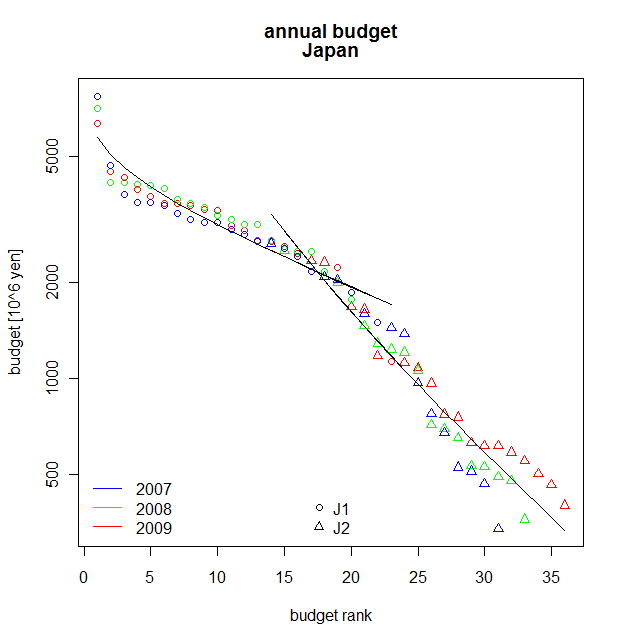
\includegraphics{fig/japan-budget.png}
		\end{center}
		\caption{Jリーグの営業支出}\label{fig:Jリーグの営業支出}
	\end{figure} %}
%s1:Jリーグの営業支出}

\section{スペインリーグの予算}\label{s1:スペインリーグの予算} %{
	Webでサッカーのスペインリーグでの予算(表\ref{tab:スペインリーグでの予算})
	が掲載されていたので、予算の分布と予算と成績との関係を調べてみた。
	\begin{equation*}\begin{array}{rcrcrl} %{
		\ln(\text{予算額}) &=& 6.2884 &-& 1.0953 & \ln(\text{予算順位}) \\
		\ln(\text{予算額}) &=& 5.9715 &-& 0.9397 & \ln(\text{リーグ戦順位}) \\
		\text{得点} &=& -14.223 &+& 8.996 & \ln(\text{予算額}) \\
		\ln(\text{失点}) &=& 4.00974 &-& 0.24946\ & \ln(\text{予算額}) \\
	\end{array}\end{equation*} %}
	予算額の値はちょっと嘘くさいと思う。このデータからほぼ
	\begin{equation*}\begin{split} %{
		\text{チームの予算額}
			=\frac{\text{予算順位一位の予算額}}{\text{チームの予算順位}}
	\end{split}\end{equation*} %}
	という関係が成り立つことになるが、あまりにもデータの値が揃いすぎている。
	普通に考えるともっとデータの値にばらつきがあると思う。

\begin{table}[!htbp]
\begin{center}
\begin{tabular}{rlrrrr} \hline
& チーム & 予算 [$10^6$ euro] & リーグ戦順位 & 得点 & 失点 \\ \hline
1 & Barcelona & 428.00 &   1 &  51 &   9 \\ 
2 & RealMadrid & 442.00 &   2 &  39 &  12 \\ 
3 & Villareal & 67.00 &   3 &  30 &  14 \\ 
4 & Valencia & 131.00 &   4 &  24 &  19 \\ 
5 & Espanol & 50.00 &   5 &  18 &  22 \\ 
6 & AtleticoMadrid & 110.00 &   6 &  27 &  19 \\ 
7 & Getafe & 24.00 &   7 &  27 &  19 \\ 
8 & AthleticBilbao & 53.10 &   8 &  25 &  27 \\ 
9 & RealSociedad & 35.00 &   9 &  22 &  26 \\ 
10 & Mallorca & 36.00 &  10 &  16 &  20 \\ 
11 & Sevilla & 90.00 &  11 &  21 &  27 \\ 
12 & Hercules & 42.00 &  12 &  18 &  22 \\ 
13 & Deportivo & 65.00 &  13 &  13 &  19 \\ 
14 & Racing & 42.00 &  14 &  13 &  23 \\ 
15 & Osasuna & 28.90 &  15 &  15 &  20 \\ 
16 & Levante & 20.00 &  16 &  18 &  26 \\ 
17 & Almeria & 28.00 &  17 &  15 &  25 \\
18 & Malaga &  &  18 &  20 &  35 \\ 
19 & Sporting & 25.00 &  19 &  12 &  23 \\ 
20 & Zaragoza & 24.50 &  20 &  13 &  26 \\ \hline
\end{tabular}
\caption{スペインリーグでの予算(2010-2011)と成績(2010/12/28)}
\label{tab:スペインリーグでの予算}
\end{center}
\end{table}

\begin{lstlisting}[caption=予算額と予算順位, label=code:予算額と予算順位]
Call:
lm(formula = log(budget) ~ log(rank))

Residuals:
     Min       1Q   Median       3Q      Max 
-0.20988 -0.05314 -0.02577  0.02378  0.52995 

Coefficients:
            Estimate Std. Error t value Pr(>|t|)    
(Intercept)   6.2884     0.1003   62.68  < 2e-16 ***
log(rank)    -1.0953     0.0453  -24.18 1.32e-14 ***
---
Signif. codes:  0 ‘***’ 0.001 ‘**’ 0.01 ‘*’ 0.05 ‘.’ 0.1 ‘ ’ 1 

Residual standard error: 0.1552 on 17 degrees of freedom
Multiple R-squared: 0.9717,     Adjusted R-squared: 0.9701 
F-statistic: 584.6 on 1 and 17 DF,  p-value: 1.320e-14
\end{lstlisting}

\begin{lstlisting}[caption=予算額とリーグ戦順位, label=code:予算額とリーグ戦順位]
Call:
lm(formula = log(budget) ~ log(rank))

Residuals:
     Min       1Q   Median       3Q      Max 
-0.96483 -0.28777  0.02317  0.22630  0.78168 

Coefficients:
            Estimate Std. Error t value Pr(>|t|)    
(Intercept)   5.9715     0.3107   19.22 5.73e-13 ***
log(rank)    -0.9397     0.1398   -6.72 3.59e-06 ***
---
Signif. codes:  0 ‘***’ 0.001 ‘**’ 0.01 ‘*’ 0.05 ‘.’ 0.1 ‘ ’ 1 

Residual standard error: 0.4828 on 17 degrees of freedom
Multiple R-squared: 0.7265,     Adjusted R-squared: 0.7104 
F-statistic: 45.16 on 1 and 17 DF,  p-value: 3.59e-06 
\end{lstlisting}

\begin{lstlisting}[caption=予算額と得点, label=code:予算額と得点]
Call:
lm(formula = goal.plus ~ log(budget))

Residuals:
    Min      1Q  Median      3Q     Max 
-10.331  -2.853  -1.402   3.863  12.632 

Coefficients:
            Estimate Std. Error t value Pr(>|t|)    
(Intercept)  -14.223      6.477  -2.196   0.0423 *  
log(budget)    8.996      1.574   5.715 2.53e-05 ***
---
Signif. codes:  0 ‘***’ 0.001 ‘**’ 0.01 ‘*’ 0.05 ‘.’ 0.1 ‘ ’ 1 

Residual standard error: 5.992 on 17 degrees of freedom
Multiple R-squared: 0.6577,     Adjusted R-squared: 0.6375 
F-statistic: 32.66 on 1 and 17 DF,  p-value: 2.528e-05
\end{lstlisting}

\begin{lstlisting}[caption=予算額と失点, label=code:予算額と失点]
Call:
lm(formula = log(goal.minus) ~ log(budget))

Residuals:
     Min       1Q   Median       3Q      Max 
-0.32176 -0.09565  0.01372  0.08273  0.40864 

Coefficients:
            Estimate Std. Error t value Pr(>|t|)    
(Intercept)  4.00974    0.20741  19.332 5.21e-13 ***
log(budget) -0.24946    0.05041  -4.948 0.000122 ***
---
Signif. codes:  0 ‘***’ 0.001 ‘**’ 0.01 ‘*’ 0.05 ‘.’ 0.1 ‘ ’ 1 

Residual standard error: 0.1919 on 17 degrees of freedom
Multiple R-squared: 0.5902,     Adjusted R-squared: 0.5661 
F-statistic: 24.49 on 1 and 17 DF,  p-value: 0.0001221 
\end{lstlisting}

%s1:スペインリーグの予算}

%\section{使う記号}\label{s1:使う記号} %{
	よく使う記号を列挙しておく。
	\begin{description}\setlength{\itemsep}{-1mm} %{
		\item[自然数]
		$0$以上の自然数を自然数を$\sizen$、$1$以上の自然数を$\sizen_+$と書く。
		$i$以上$j$以下の自然数の集合を$i..j$と書く。$i..j$と書いて$j<i$の場合
		は空集合とする。
		\item[よく使う集合]
		元が一つもない集合を$\mybf{0}$、元が一つだけの集合を$\mybf{1}$と書く。
		整数を$\sei$、実数を$\jitu$、複素数を$\fukuso$と書く。
		\item[ブーリアン]
		ブーリアンを$\bool=\set{0,1}$と書く。ブーリアンの論理和を$\mybiop{+}$、
		論理積を$\mybiop{\myspace}$と書く。
		\item[冪集合]
		集合$A$に対して、空集合も含む$A$の冪集合を$PA$、空集合を含まない
		$A$の冪集合を$P_+A$と書く。
		\item[文字列集合]
		集合$A$に対して、$A$の元を文字とする長さ$0$以上の文字列の集合を$WA$、
		長さ$1$以上の文字列の集合を$W_+A$と書く。
		\item[半モジュール]
		集合$A$、半環$R$に対して、$A$を基底とする$R$係数自由半モジュールを
		$RA$と書く。
		\item[写像]
		集合$A,B$に対して、$A$から$B$への写像全体のつくる空間を$\set{A\to B}$
		や$\myop{map}(A,B)$と書く。
		\item[デルタ関数]
		論理式を$\jump{}$で囲ってデルタ関数を表す。
		\begin{equation*}\begin{split} %{
			\jump{\text{expression}} &= \begin{cases}
				1, &\text{ iff }\text{expression is true} \\
				0, &\text{ otherwise } \\
			\end{cases}
		\end{split}\end{equation*} %}
	\end{description} %}

\subsection{文字列集合}\label{s2:文字列集合} %{
	$A$を集合、$WA$を$A$の元を文字とする文字列の集合とする。
	\begin{itemize}\setlength{\itemsep}{-1mm} %{
		\item 長さ$0$の文字列、つまり空の単語を$1_W$と書く。
		\item 文字列は通常の直積の元の書き方$(a_1,a_2,\dots,a_m)$の他に
		$\bakko{a_1a_2\cdots a_m}$というように文字を並べてカギ括弧で囲って
		表すこともある。
		\item 文字列$w_1$と$w_2$の連結(juxtaposition)を$w_1*w_2$と書く。
		例えば、$[abc]*[de]=[abcde]$となる。
		\item 文字列$w$に含まれる文字$a$の数を$\sharp_aw$と書く。
		例えば、$\sharp_a[abcba]=2$となる。
	\end{itemize} %}

	$R$を半環、$RWA$を$WA$を基底とする$R$係数自由半モジュールとする。
	余積$\Delta_*$を次のように定義する。
	\begin{equation}\label{eq:連結余積の定義}\begin{array}{rcll} %{
		\Delta_*1_W &=& 1_W\otimes1_W \\
		\Delta_*[a] &=& [a]\otimes1_W+1_W\otimes[a] & \text{for all }a\in A \\
		\Delta_*(w_1*w_2*\cdots*w_m) &=& (\Delta_*w_1)*(\Delta_*w_2)*\cdots
			*(\Delta_*w_m) & \text{for all }w_1,w_2,\dots,w_m\in WA
	\end{array}\end{equation} %}
	ここで、テンソル積に対する積を
	$(w_1\otimes w_2)*(w_3\otimes w_4)=(w_1*w_3)\otimes(w_2*w_4)$とした。
	定義より余積$\Delta_*$と積$\mybiop{*}$は互いに準同型となっている。
	この余積$\Delta_*$を連結余積と書くことにする。

	\begin{definition}[連結余積]\label{def:連結余積} %{
		式\eqref{eq:連結余積の定義}で定義された余積$\Delta_*$を連結余積
		ということにする。
	\end{definition} %def:連結余積}
%s2:文字列集合}
%s1:使う記号}

\section{球を箱に入れる仕方の数}\label{s1:球を箱に入れる仕方の数} %{
	球を箱に入れる仕方の数を次のバリエーションで考えてみる。
	考え方は文献\cite{html:iga.math}に従う。
	\begin{itemize}\setlength{\itemsep}{-1mm} %{
		\item 球が区別つく場合とつかない場合
		\item 箱が区別つく場合とつかない場合
		\item 空の箱を許すか許さないか
	\end{itemize} %}
	次のパターンを使って、空の箱を許す場合と許さない場合のどちらか簡単な
	方で球を箱に入れる仕方の数を計算して他方を導くことが多い。
	\begin{equation}\label{eq:空箱ありは空箱なしの直和}\begin{split} %{
		k\text{箱に空箱を許して入れる仕方} 
		&= 1\text{箱に空箱を許さず入れる仕方} \\
		&+ 2\text{箱に空箱を許さず入れる仕方} \\
		&+ \cdots \\
		&+ k\text{箱に空箱を許さず入れる仕方}
	\end{split}\end{equation} %}
\subsection{球と箱が区別つく場合}\label{s2:球と箱が区別つく場合} %{
\subsubsection{空箱を許す場合}\label{s3:空箱を許す場合} %{
	球$1$を箱$a_1$に入れ、球$2$を箱$a_2$に入れ、、、球$n$を箱$a_n$に入れた
	状態を文字列$[a_1a_2\cdots a_m]$で表す。すると、$n$個の球を$k$個の箱へ
	入れる仕方は、$1..n$を文字とする長さ$n$の文字列で表すことができることが
	わかる。したがって、$n$個の球を$k$個の箱へ入れた状態空間は$(1..k)^n$
	になることがわかる。また、入れ方の仕方の数は$k^n$になることもわかる。
%s3:空箱を許す場合}
\subsubsection{空箱を許さない場合}\label{s3:空箱を許さない場合} %{
	$n$個の球を$k$個の箱に入れる仕方は、文字列集合$(1..k)^n$を、
	文字列の中に$1..k$のすべての文字が含まれるものに制限したものになる。
	これを$\mycal{A}_k^n$と書く。
	\begin{equation*}\begin{split} %{
		\mycal{A}_k^n &= \set{w\in (1..k)^n
			\bou 1\le \sharp_aw \quad\text{for all }a\in (1..k)}
	\end{split}\end{equation*} %}
	$n<k$の場合は、空の箱を許さない入れ方は不可能なので、$\mycal{A}_k^n$
	は空集合と定義する。

	$\mycal{A}_k^n$は集合として由緒正しいものである。集合同型の意味で
	次の式が成り立つ。
	\begin{equation*}\begin{split} %{
		(1..k)^n &\simeq \set{1..n\to 1..k} \\
		\mycal{A}_k^n &\simeq \set{f:1..n\to 1..k\bou f\text{は}\myop{onto}} \\
	\end{split}\end{equation*} %}

	$\mycal{A}_k^n$の大きさを調べる。まず、簡単な例から始める。
	$\mycal{A}_2^3$は次のようになり、
	\begin{equation*}\begin{split} %{
		(1..2)^3 &= \set{[111],[112],[121],[122],[211],[212],[221],[222]} \\
		\mycal{A}_2^3 &\simeq \set{[112],[121],[122],[211],[212],[221]} \\
		\mycal{A}_1^3 &\simeq \set{[111]} \\
		\mycal{A}_1^3 &\simeq \set{[222]} \\
	\end{split}\end{equation*} %}
	$\zettai{(1..2)^3}=\zettai{\mycal{A}_2^3}+2\zettai{\mycal{A}_1^3}$と
	書けることがわかる。\footnote{
		半モジュールで$\sizen(1..2)^3\simeq
		\sizen\mycal{A}_2^3\oplus\sizen\mycal{A}_1^3\oplus\sizen\mycal{A}_1^3$
		と書いた方がわかり易いかもしれない。
	}

	この関係の一般の場合がパターン\eqref{eq:空箱ありは空箱なしの直和}である。
	ただし、空でない$p$個の箱を選びだす仕方は$\binom{k}{p}$通りある。
	したがって、$A_k^n=\zettai{\mycal{A}_k^n}$と書くと、任意の
	$k,n\in\sizen_+$に対して次の漸化式が成り立つ。
	\begin{equation}\label{eq:空箱ありの仕方の数は空箱なし仕方の数の和}\begin{split} %{
		k^n = \sum_{p\in1..k}\binom{k}{p}A_p^n
	\end{split}\end{equation} %}
	ただし、$n<k$の場合は$A_k^n=0$である。この漸化式を行列の形で書くと
	$K = CA$となる。ここで、$K,C,B$はそれぞれ次のように定義した。
	\begin{equation*}\begin{split} %{
		K = \begin{pmatrix}
			k^n \\ (k-1)^n \\ \vdots \\ 1^n
		\end{pmatrix} 
		,\quad B = \begin{pmatrix}
			A_k^n \\ A_{k-1}^n \\ \vdots \\ A_1^n
		\end{pmatrix}
		,\quad C = \begin{pmatrix}
			\binom{k}{0} & \binom{k}{1} & \cdots & \binom{k}{k-1} \\
			0 & \binom{k-1}{0} & \cdots & \binom{k-1}{k-2} \\
			\vdots & \vdots & \cdots & \vdots \\
			0 & 0 & \cdots & \binom{1}{0} \\
		\end{pmatrix} 
	\end{split}\end{equation*} %}
	行列$C$の逆行列が求まれば$C^{-1}K$によって$B$が求まる。
	$C$の行列式は$1$だから逆行列を持ち次のようになる。
	\begin{equation*}\begin{split} %{
		C^{-1} = \begin{pmatrix}
			\binom{k}{0} & -\binom{k}{1} & \cdots & (-)^{k-1}\binom{k}{k-1} \\
			0 & \binom{k-1}{0} & \cdots & (-)^{k-2}\binom{k-1}{k-2} \\
			\vdots & \vdots & \cdots & \vdots \\
			0 & 0 & \cdots & \binom{1}{0} \\
		\end{pmatrix}
	\end{split}\end{equation*} %}
	したがって漸化式が解けて、任意の$k,n\in\sizen_+$に対して次のようになる。
	\begin{equation}\label{eq:分配の大きさ}\begin{split} %{
		A_k^n &= \begin{cases}
			\alpha_k^n, &\text{ iff }k\le n \\
			0, &\text{ otherwise } \\
		\end{cases} \\
		\alpha_k^n &= \sum_{p\in1..k}(-)^{k-p}\binom{k}{p}p^n
	\end{split}\end{equation} %}
%s3:空箱を許さない場合}
%s2:球と箱が区別つく場合}
\subsection{球が区別つき、箱が区別つかない場合}\label{s2:球が区別つき、箱が区別つかない場合} %{
\subsubsection{空箱を許す場合}\label{s3:空箱を許す場合} %{
	球と箱が区別つかない場合の仕方$(1..k)^n$を箱の並び順を対称化すれば、
	この場合の仕方が得られる。式で書くと、$S_k$を$k$次対称群として、
	同値関係$\sim_\sqcup$を次のように定義し、
	\begin{equation*}\begin{split} %{
		[a_1a_2\cdots a_n]
		\sim_\sqcup [(\sigma a_1)(\sigma a_2)\cdots(\sigma a_n)]
		\quad\text{for all }\sigma\in S_k
	\end{split}\end{equation*} %}
	商集合$(1..k)^n/\sim_\sqcup$がこの場合の仕方となる。

	$(1..k)^n/\sim_{\sqcup}$の大きさは、単純に$(1..k)^n$の大きさを$S_k$の
	大きさで割ったものにならない。一般には次のようになる。
	\begin{equation*}\begin{split} %{
		\frac{\zettai{(1..k)^n}}{\zettai{S_k}} 
		= \frac{k^n}{k!}\le \zettai{(1..k)^n/\sim_{\sqcup}}
	\end{split}\end{equation*} %}
	$(1..3)^3$の例で説明する。球$1$が箱$1$に、球$2$が箱$2$に、球$3$が箱$1$
	に入った状態を$\bakko{\set{13}\set{2}\set{}}$と書くことにする。
	この記法を使うと、$\bakko{\set{1}\set{2}\set{3}}$の$\sim_\sqcup$同値類
	は次の$6$個なのに対し、
	\begin{equation*}\begin{array}{ccc} %{
		\bakko{\set{1}\set{2}\set{3}} & \bakko{\set{1}\set{3}\set{2}} 
			& \bakko{\set{2}\set{1}\set{3}} \\
		\bakko{\set{2}\set{3}\set{1}} & \bakko{\set{3}\set{1}\set{2}} 
			& \bakko{\set{3}\set{2}\set{1}}
	\end{array}\end{equation*} %}
	$\bakko{\set{123}\set{}\set{}}$の$\sim_\sqcup$同値類は次の$3$個
	しかない。
	\begin{equation*}\begin{array}{ccc} %{
		\bakko{\set{123}\set{}\set{}} & \bakko{\set{}\set{123}\set{}}
			& \bakko{\set{}\set{}\set{123}}
	\end{array}\end{equation*} %}
	この例は空箱同士を入れ替えても$(1..k)^n$の状態が変わらない例になって
	いる。箱を入れ替える操作で不変になっている$(1..k)^n$の元があるために、
	単純に$k^n/k!$が$(1..k)^n/\sim_\sqcup$の大きさにならない理由である。

	$(1..k)^n/\sim_\sqcup$の大きさを直接計算することが難しいので、
	空箱を許さない場合に球を箱に入れる仕方の数が計算できることを祈りつつ、
	パターン\eqref{eq:空箱ありは空箱なしの直和}を使うと、次のようになる。
	\begin{equation*}\begin{split} %{
		\zettai{(1..k)^n/\sim_\sqcup}
		= \sum_{p=1..k}
		\text{空箱を許さずに$n$個の球を$k$個の箱に入れる仕方の数}
	\end{split}\end{equation*} %}
%s3:空箱を許す場合}
\subsubsection{空箱を許さない場合}\label{s3:空箱を許さない場合} %{
	空箱を許す場合\ref{s3:空箱を許す場合}と同様に、箱が区別つく場合の
	仕方$\mycal{A}_k^n$を箱について対称化すれば、この場合の仕方
	$\mycal{B}_k^n=\mycal{A}_k^n/\sim_\sqcup$が得られる。
	定義より$\mycal{A}_k^n$に箱を入れ替える操作で不変な状態はない。
	\begin{equation}\label{eq:空箱を許さない場合の効果的な箱変換}\begin{split} %{
		[(\sigma a_1)(\sigma a_2)\cdots(\sigma a_n)] = [a_1a_2\cdots a_n]
			\implies \sigma = \myid \\
		\quad\text{for all }[a_1a_2\cdots a_n]\in\mycal{A}_k^n
			,\;\sigma\in S_k
	\end{split}\end{equation} %}
	したがって、$\mycal{B}_k^n$の大きさは、単純に$\mycal{A}_k^n$の大きさを
	$S_k$の大きさで割ったものになる。
	\begin{equation}\label{eq:第二種スターリング数}\begin{split} %{
		\zettai{\mycal{B}_k^n} = \begin{cases}
			\frac{1}{k!}A_k^n, &\text{ iff }k\le n \\
			0, &\text{ otherwise } \\
		\end{cases} \quad\text{for all }k,n\in \mybf{N}
	\end{split}\end{equation} %}
	空の箱を許さない場合は、空の箱を許す場合と異なり、箱が区別つく場合の
	状態空間に箱の変換群が効果的に作用している
	(式\eqref{eq:空箱を許さない場合の効果的な箱変換})
	ことが大きさの計算が容易になっているミソである。

	ここで求めた集合の大きさ$\zettai{\mycal{B}_k^n}$のことを第二種
	スターリング数という。

	\begin{definition}[第二種スターリング数(Stirling number of 2nd kind)]\label{def:第二種スターリング数} %{
		式\eqref{eq:第二種スターリング数}の$\zettai{\mycal{B}_k^n}$を
		第二種スターリング数という。
	\end{definition} %def:第二種スターリング数}
%s3:空箱を許さない場合}
%s2:球が区別つき、箱が区別つかない場合}
\subsection{球の区別がつかず、箱の区別がつく場合}\label{s2:球の区別がつかず、箱の区別がつく場合} %{
\subsubsection{空箱を許す場合}\label{s3:空箱を許す場合} %{
	この場合の球を箱に入れる仕方の数は巧妙な方法で求められる。
	\begin{itemize}\setlength{\itemsep}{-1mm} %{
		\item $k$個の箱に一つづつ球を入れた状態でスタートする。
		\item $n$個の球を箱に分配する。
		\item すると、$k$個すべての箱が空でなく、$n$個の球を箱に仕方の数と
		同数の状態が出現する。
	\end{itemize} %}
	したがって、$n$個の球を$k$個の箱に空箱を許して入れる仕方の数は、
	$n+k$個の球を$k$個の箱に空箱を許さず入れる仕方の数になる。
%s3:空箱を許す場合}
\subsubsection{空箱を許さない場合}\label{s3:空箱を許さない場合} %{
	この場合の球を箱へ入れる仕方$\mycal{C}_k^n$は、$n=a_1+a_2+\cdots+a_k$
	となる$\sizen_+$を文字とする長さ$k$の文字列$[a_1a_2\cdots a_k]$全体
	の作る集合となる。式で書くと次のようになる。
	\begin{equation*}\begin{split} %{
		\mycal{C}_k^n = \set{[a_1a_2\cdots a_k]\in \mybf{N}_+^k
			\bou a_1+a_2+\cdots+a_k=n}
	\end{split}\end{equation*} %}
	$\mycal{C}_k^n$の大きさは次のようにして求めることができる。
	\begin{itemize}\setlength{\itemsep}{-1mm} %{
		\item $1$の間に$\square$を挟んで次のように書く。
		\begin{equation*}\begin{split} %{
			\underbrace{1\square 1\square \cdots \square 1}
				_{1\text{が}n\text{個}}
		\end{split}\end{equation*} %}
		\item $\square$に$+$または$\myspace$を書き込むと$\mycal{C}_k^n$
		の元となる。
	\end{itemize} %}
	例えば$n=3$であれば次のようになる。
	\begin{equation*}\begin{array}{rclclcl} %{
		1\square 1\square 1
		&\xrightarrow{(++)}& 1+1+1 &=& 3 &\in& \mycal{C}_1^3 \\
		&\xrightarrow{(+,\myspace)}& 1+1\myspace 1 &=& 2\myspace 1 
			&\in& \mycal{C}_2^3 \\
		&\xrightarrow{(\myspace,+)}& 1\myspace 1+1 &=& 1\myspace 2 
			&\in& \mycal{C}_2^3 \\
		&\xrightarrow{(\myspace,\myspace)}& 1\myspace 1\myspace 1
			&=& 1\myspace 1\myspace 1 &\in& \mycal{C}_3^3 \\
	\end{array}\end{equation*} %}
	一般の$\mycal{C}_k^n$では、$n-1$個の$\square$の中から$k-1$個を選択
	して、そこに$\myspace$を書き込むと$\mycal{C}_k^n$の状態ができる。
	したがって、$\mycal{C}_k^n$の大きさは次のようになることがわかる。
	\begin{equation*}\begin{split} %{
		\zettai{\mycal{C}_k^n} = \begin{cases}
			\binom{n-1}{k-1}, &\text{ iff } k\le n \\
			0, &\text{ otherwise } \\
		\end{cases} \quad\text{for all }k,n\in \mybf{N}_+
	\end{split}\end{equation*} %}
	また、この構成方法より、$\sum_{k\in(1..n)}\mycal{C}_k^n$は、
	集合$\set{+,\myspace}$を文字とする長さ$n-1$の文字列全体と集合同型となる
	ことがわかり、次の式が導かれる。
	\begin{equation*}\begin{split} %{
		2^{n-1} = \sum_{k\in(1..n)}\binom{n-1}{k-1}
	\end{split}\end{equation*} %}

	$\mycal{C}_k^n$の状態を$n$の合成という。

	\begin{definition}[自然数の合成(Composition)]\label{def:自然数の合成(Composition)} %{
		$\mycal{C}_k^n$の元を長さ$n$の$k$の合成という。
	\end{definition} %def:自然数の合成(Composition)}
%s3:空箱を許さない場合}
%s2:球の区別がつかず、箱の区別がつく場合}
\subsection{まとめ}\label{s2:まとめ} %{
	$n$個の球を$k$個の箱に分配する仕方を次のバリエーションごとに調べた。
	\begin{itemize}\setlength{\itemsep}{-1mm} %{
		\item 球が区別つく場合とつかない場合
		\item 箱が区別つく場合とつかない場合
		\item 空の箱を許すか許さないか
	\end{itemize} %}
	それらをまとめると、$n$個の球を$k$個の箱に入れる仕方の数は次のように
	なる。
	\begingroup
	\renewcommand{\arraystretch}{1.5}
	\begin{equation}\label{eq:球を箱に入れる仕方の数の表}\begin{array}{cccc} %{
		\text{球の区別} & \text{箱の区別} & \text{空箱} & \text{仕方の数} \\
		\text{有り} & \text{有り} & \text{有り} & k^n \\
		\text{有り} & \text{有り} & \text{無し} & k!B_k^n \\
		\text{有り} & \text{無し} & \text{有り} & \sum_{k\in1..n}B_k^n \\
		\text{有り} & \text{無し} & \text{無し} & B_k^n \\
		\text{無し} & \text{有り} & \text{有り} & \binom{n+k-1}{k-1} \\
		\text{無し} & \text{有り} & \text{無し} & C_k^n \\
	\end{array}\end{equation} %}
	\endgroup
	ここで、$B_k^n$と$C_k^n$はそれぞれ次のように定義される。
	\begin{equation*}\begin{split} %{
		B_k^n &= \begin{cases}
			\frac{1}{k!}\sum_{p\in(1..k)}(-)^{k-p}\binom{k}{p}p^n, &\text{ iff }k\le n \\
			0, &\text{ otherwise } \\
		\end{cases} \\
		C_k^n &= \begin{cases}
			\binom{n-1}{k-1}, &\text{ iff }k\le n \\
			0, &\text{ otherwise } \\
		\end{cases} \\
	\end{split}\end{equation*} %}
%s2:まとめ}
%s1:球を箱に入れる仕方の数}

\section{球を箱に空箱を許さず入れる仕方}\label{s1:球を箱に空箱を許さず入れる仕方} %{
	前節に引き続き、球を箱に空箱を許さず入れる仕方を考える。この節では
	球も箱も区別できない場合も考える。$n$個の球を$k$個の箱に入れる仕方を
	次のように定義する。
	\begin{itemize}\setlength{\itemsep}{-1mm} %{
		\item 球と箱も区別つく場合を$\mycal{A}_k^n$とする。
		\item 球が区別つき、箱が区別つかない場合を$\mycal{B}_k^n$とする。
		\item 球が区別つかず、箱が区別つく場合を$\mycal{C}_k^n$とする。
		\item 球と箱も区別つかない場合を$\mycal{P}_k^n$とする。
	\end{itemize} %}
	箱を対称化する操作を$\pi_\sqcup$、球を対称化する操作を$\pi_\circ$
	と書く。それぞれの集合は次の$\myop{onto}$写像の可換図によっても表される。
	\begin{equation*}\xymatrix@C=6pc{
		\mycal{A}_k^n \ar[r]_{\text{球を対称化}}^{\pi_\circ}
		 \ar[d]_{\text{箱を対称化}}^{\pi_\sqcup}
			& \mycal{C}_k^n \ar[d]_{\text{箱を対称化}}^{\pi_\sqcup} \\
		\mycal{B}_k^n \ar[r]_{\text{球を対称化}}^{\pi_\circ} & \mycal{P}_k^n \\
	}\end{equation*}
	前節の結果をもう一度書くと、$n$個の球を$k$個の箱に入れる仕方の数は
	次のようになる。
	\begingroup
	\renewcommand{\arraystretch}{1.5}
	\begin{equation*}\begin{array}{cccc} %{
		\text{球の区別} & \text{箱の区別} & \text{集合} & \text{集合の大きさ} \\
		\text{有り} & \text{有り} & \mycal{A}_k^n & k!B_k^n \\
		\text{有り} & \text{無し} & \mycal{B}_k^n & B_k^n \\
		\text{無し} & \text{有り} & \mycal{C}_k^n & C_k^n \\
		\text{無し} & \text{無し} & \mycal{P}_k^n & \text{不明} \\
	\end{array}\end{equation*} %}
	\endgroup
	\begin{equation*}\begin{split} %{
		B_k^n &= \begin{cases}
			\frac{1}{k!}\sum_{p\in(1..k)}(-)^{k-p}\binom{k}{p}p^n, 
				&\text{ iff }k\le n \\
			0, &\text{ otherwise } \\
		\end{cases} \\
		C_k^n &= \begin{cases}
			\binom{n-1}{k-1}, &\text{ iff }k\le n \\
			0, &\text{ otherwise } \\
		\end{cases} \\
	\end{split}\end{equation*} %}
	$\mycal{P}_k^n$は$n$の$k$分割といい、その大きさを表す簡単な式はない
	ようだ。

	$\mycal{X}\in\set{\mycal{A},\mycal{B},\mycal{C},\mycal{P}}$として、
	次のように拡張して添え字$k,n$を自然数$\sizen$にとれるようにしておく。
	\begin{itemize}\setlength{\itemsep}{-1mm} %{
		\item $\mycal{X}_0^0=\set{\bullet}$とする。
		\item 任意の$n\in\sizen_+$に対して$\mycal{X}_0^n=\emptyset$とする。
		\item 任意の$k\in\sizen_+$に対して$\mycal{X}_k^0=\emptyset$とする。
		\item 任意の$k<n\in\sizen$に対して$\mycal{X}_k^n=\emptyset$とする。
	\end{itemize} %}
	記号$\bullet$は箱も球もない状態を表す。
	また、
	\begin{itemize}\setlength{\itemsep}{-1mm} %{
		\item $\mycal{X}_*^n=\sum_{k\in0..n}\mycal{X}_k^n$、
		\item $\mycal{X}_*^*=\sum_{n\in\sizen}\mycal{X}_*^n$
	\end{itemize} %}
	と書くことにする。

	$\mycal{A}_k^n$の元を$WW_+(1..k)$の部分集合として$2$次元の文字列で
	次のように書き表すことにする。
	\begin{equation*}\begin{split} %{
		\bigl[[1][4][23]\bigr] = \bigl((1),(4),(2,3)\bigr) 
		= \left\{\begin{array}{l}
			\text{箱$1$に球$1$} \\
			\text{箱$2$に球$4$} \\
			\text{箱$3$に球$2$と球$3$} \\
			\end{array}\right\}\text{入った状態}
	\end{split}\end{equation*} %}
	$\mycal{B}_k^n$の元を$WW_+(1..k)$の部分集合として$2$次元の文字列で
	表す場合は、箱に入っている球の最も小さい数字によって、箱を左から右へ順に
	並べるものとする。例えば次のようになる。
	\begin{equation*}\begin{split} %{
		\bigl[[1][4][23]\bigr]\in\mycal{A}_3^4 
			\xmapsto{\pi_\circ} \bigl[[1][23][4]\bigr]\in\mycal{B}_3^4
	\end{split}\end{equation*} %}
	同様に、$\mycal{C}_k^n$の元を$W(1..n)$の部分集合として文字列で
	次のように書き表すことにする。
	\begin{equation*}\begin{split} %{
		[121] = (1,2,1) = \left\{\begin{array}{l}
			\text{箱$1$に球が$1$個} \\
			\text{箱$2$に球が$2$個} \\
			\text{箱$3$に球が$1$個} \\
			\end{array}\right\}\text{入った状態}
	\end{split}\end{equation*} %}
	$\mycal{P}_k^n$の元を$W(1..n)$の部分集合として文字列で表す場合は、
	箱に入っている球の数が右から左に小さくなるように並べるとする。例えば
	次のようになる。
	\begin{equation*}\begin{split} %{
		[121]\in\mycal{C}_3^4 
			\xmapsto{\pi_\sqcup} [211]\in\mycal{P}_3^4
	\end{split}\end{equation*} %}

	集合$\mycal{B}_k^n$と$\mycal{P}_k^n$の元を図形で表す方法を定義しておく。

	\begin{definition}[ヤング図形]\label{def:ヤング図形} %{
		任意の$n\in\mybf{N}_+$に対して次の条件を満たす二次元配列を
		$n$次のヤング図形という。
		\begin{itemize}\setlength{\itemsep}{-1mm} %{
			\item 各行の長さが一定とは限らない。
			\item 空の行を含まない。
			\item 升目の総数が$n$である。
			\item 各行の長さは上から下へ同じか減少していく。
		\end{itemize} %}
	\end{definition} %def:ヤング図形}

	ヤング図形は歴史も長くいろいろな場面で使われるために、次のような
	慣用的な書き方がある。
	\begin{itemize}\setlength{\itemsep}{-1mm} %{
		\item ヤング図形は記号$\lambda$で書かれる。
		\item ヤング図形$\lambda\vdash n$は$n$次のヤング図形を表す。
		\item ヤング図形$\lambda=[\lambda_1\lambda_2\cdots\lambda_k]$
		とは、$1$行目の長さが$\lambda_1$、$2$行目の長さが$\lambda_2$、、、$k$
		行目の長さが$\lambda_k$という$k$行のヤング図形を表すものとする。
		\item 分割$n=\lambda_1+\lambda_2+\dots+\lambda_k$のヤング図形とは、
		$1$行目の長さが$\lambda_1$、$2$行目の長さが$\lambda_2$、、、$k$行目の
		長さが$\lambda_k$という$k$行のヤング図形を表すものとする。
	\end{itemize} %}

	\begin{definition}[分配盤]\label{def:分配盤} %{
		任意の$n\in\mybf{N}_+$に対して次の条件を満たす二次元配列を
		$n$次の分配盤と言うことにする。
		\begin{itemize}\setlength{\itemsep}{-1mm} %{
			\item 各行の長さが一定とは限らない。
			\item 空の行を含まない。
			\item 升目の総数が$n$である。
			\item 升目には$1$から$n$までの数字が重複無く書かれている。
			\item 一列目の数字は上から下へ増加していく。
			\item 各行で数字は左から右へ増加していく。
		\end{itemize} %}
	\end{definition} %def:分配盤}

	ヤング図形の行のことを箱ともいう。分配盤の行のことを箱、升目の中に
	書かれている数字ことを球のラベルともいう。
	$n$次$k$行のヤング図形全体の作る集合が$\mycal{P}_k^n$となり、
	$n$次$k$行の分配盤全体の作る集合が$\mycal{B}_k^n$となる。

	以下の節では、順不同で球を箱に入れる仕方に関連する話題を書くことにする。
	
\subsection{対称化の逆の大きさ}\label{s2:対称化の逆の大きさ} %{
	対称化$\pi_\sqcup$と$\pi_\circ$の逆写像の大きさをそれぞれの
	次のようになる。
	\begin{itemize}\setlength{\itemsep}{-1mm} %{
		\item $\pi_\sqcup:\mycal{A}_k^n\to\mycal{B}_k^n$の場合、
		逆写像の大きさは次のようになる。
		\begin{equation*}\begin{split} %{
			\zettai{\pi_\circ^{-1}t} = k! \quad\text{for all }t\in\mycal{B}_k^n
		\end{split}\end{equation*} %}
		例えば次のようになる。
		\begin{equation*}\begin{split} %{
			\pi_\circ^{-1}\young(12,3) = \Set{\bigl[[12][3]\bigr]
				,\; \bigl[[3][12]\bigr]}
		\end{split}\end{equation*} %}
		\item $\pi_\circ:\mycal{A}_k^n\to\mycal{C}_k^n$の場合、
		逆写像の大きさは次のようになる。
		\begin{equation*}\begin{split} %{
			\zettai{\pi_\circ^{-1}[n_1n_2\cdots n_k]} 
				= \frac{n!}{n_1!n_2!\cdots n_k!}
				\quad\text{for all }[n_1n_2\cdots n_k]\in\mycal{C}_k^n
		\end{split}\end{equation*} %}
		例えば次のようになる。
		\begin{equation*}\begin{split} %{
			\pi_\circ^{-1}[21] = \Set{[12][3]\bigr],\;\bigl[[23][1]\bigr]
				,\;\bigl[[13][2]}
		\end{split}\end{equation*} %}
		\item $\pi_\sqcup:\mycal{B}_k^n\to\mycal{P}_k^n$の場合、
		逆写像の大きさは次のようになる。
		\begin{equation}\label{eq:分配盤とヤング図形の対応数}\begin{split} %{
			\zettai{\pi_\circ^{-1}[\lambda_1\lambda_2\cdots\lambda_k]}
			= \frac{1}{S_\lambda}\frac{n!}{\lambda_1!\lambda_2!\cdots \lambda_k!}
			\quad\text{for all }\lambda
				=[\lambda_1\lambda_2\cdots\lambda_k]\in\mycal{P}_k^n
		\end{split}\end{equation} %}
		ここで、$S_\lambda$はヤング図形$\lambda$の行の重複に対応した数で、
		次のように定義される。
		\begin{equation*}\begin{split} %{
			S:\yng(3,3,2,1,1,1)\mapsto 2!1!3!
		\end{split}\end{equation*} %}
		$\pi_\circ^{-1}$の例は次のようになる。
		\begin{equation*}\begin{split} %{
			\pi_\circ^{-1}\yng(2,1,1) &= \Set{\young(12,3,4),\; \young(1,23,4)
				,\; \young(13,2,4),\; \young(14,2,3),\; \young(1,24,3)
				,\; \young(1,2,34)} \\
			\pi_\circ^{-1}\yng(3,1) &= \Set{\young(123,4),\; \young(124,3)
				,\; \young(134,2),\; \young(1,234)}
		\end{split}\end{equation*} %}
		\item $\pi_\sqcup:\mycal{P}_k^n\to\mycal{C}_k^n$の場合、
		逆写像の大きさは次のようになる。
		\begin{equation*}\begin{split} %{
			\pi_\sqcup^{-1}[\lambda_1\lambda_2\cdots\lambda_k]
			= \frac{k!}{S_\lambda} \quad\text{for all }
				[\lambda_1\lambda_2\cdots\lambda_k]\in\mycal{P}_k^n
		\end{split}\end{equation*} %}
		例えば次のようになる。
		\begin{equation*}\begin{split} %{
			\pi_\sqcup^{-1}\yng(3,2,1) &= \Set{[123],\; [132],\; [213],\; [231]
			,\; [312],\; [321]} \\
			\pi_\sqcup^{-1}\yng(2,1,1) &= \Set{[211],\; [121],\; [112]} \\
			\pi_\sqcup^{-1}\yng(3,1) &= \Set{[31],\; [13]}
		\end{split}\end{equation*} %}
	\end{itemize} %}
	対称化$\pi_\sqcup$と$\pi_\circ$の逆写像の大きさを図(可換図ではない)
	で書くと次のようになる。
	\begin{equation*}\xymatrix@R=4pc@C=8pc{
		\mycal{A}_k^n
			& \mycal{C}_k^n \ar@{|.>}[l]
				^{\frac{n!}{\lambda_1!\lambda_2!\cdots \lambda_k!}}
				_{\pi_\circ^{-1}} \\
		\mycal{B}_k^n \ar@{|.>}[u]^{k!}_{\pi_\sqcup^{-1}} 
			& (\lambda_1,\lambda_2,\dots,\lambda_k)
			\ar@{|.>}[l]^{\frac{1}{S_\lambda}
				\frac{n!}{\lambda_1!\lambda_2!\cdots \lambda_k!}}_{\pi_\circ^{-1}}
			\ar@{|.>}[u]^{\frac{k!}{S_\lambda}}_{\pi_\sqcup^{-1}} \\
	}\end{equation*}
%s2:対称化の逆の大きさ}
\subsection{球を箱に入れる仕方の列挙}\label{s2:球を箱に入れる仕方の列挙} %{
	まず、分配盤に対する自然な成長を定義する。

	\begin{definition}[分配盤の自然な成長]\label{def:分配盤の自然な成長} %{
		分配盤の$k$行目に新しい球を追加する操作を$k$行に対する自然な成長と
		いい、$\myop{grow}_k$と書く。また、$\myop{grow}_0$を新たに行を
		付け足してその行に新しい球を入れる操作とする。
		行に対する自然な成長をベクトル空間$\jitu\mycal{B}_*^*$の
		線形写像に拡張して、次のように定義された線形写像
		$\myop{grow}:\jitu\mycal{B}_*^*\to\jitu\mycal{B}_*^*$を分配盤の
		自然な成長という。
		\begin{equation*}\begin{split} %{
			\myop{grow}t = \sum_{k\in0..k}\myop{grow}_kt
			\quad\text{for all }t\in\mycal{B}_k^n,\;k,n\in\sizen
		\end{split}\end{equation*} %}
	\end{definition} %def:分配盤の自然な成長}

	行に対する自然な成長$\myop{grow}_k,\;1\le k$は任意の$n\in\sizen$の
	$\mycal{B}_0^n,\mycal{B}_1^n,\dots,\mycal{B}_k^n$に対してのみに
	定義され、$\myop{grow}_0$はすべて$\mycal{B}_*^*$に対して定義される。

	\begin{example}[分配盤の自然な成長]\label{eg:分配盤の自然な成長} %{
		行に対する自然な成長は次のようになり、
		\begin{equation*}\begin{split} %{
			\myop{grow}_0\young(1,2) &= \young(1,2,3) \\
			\myop{grow}_1\young(1,2) &= \young(13,2) \\
			\myop{grow}_2\young(1,2) &= \young(1,23) \\
		\end{split}\end{equation*} %}
		自然な成長は次のようになる。
		\begin{equation*}\begin{array}{rrl} %{
			\myop{grow}\young(1,2) &= \young(1,2,3) + \young(13,2) + \young(1,23)
		\end{array}\end{equation*} %}
	\end{example} %eg:分配盤の自然な成長}

	ヤング図形に対しても自然な成長を分配盤と同様に定義する。ただし、
	ヤング図形$\mycal{P}$の行に対する自然な成長を行うと成長した行の長さが
	上の行の長さを超えてしまうことがあるので、その際は行を入れ替えて
	ヤング図形の形に直すものとする。

	\begin{definition}[ヤング図形の自然な成長]\label{def:ヤング図形の自然な成長} %{
		ヤング図形の$k$行目の長さ一つ増加させる操作を$k$行に対する自然な成長
		といい、$\myop{grow}_k$と書く。ただし、$k$行目の長さ一つ増加させた
		結果、$k$行目の長さ$k-1$行目の長さより長くなった場合は、行を入れ替えて
		ヤング図形の形に書き直すものとする。また、$\myop{grow}_0$を新たに行を
		付け足してその行に新しい球を入れる操作とする。
		行に対する自然な成長をベクトル空間$\jitu\mycal{P}_*^*$の
		線形写像に拡張して、次のように定義された線形写像
		$\myop{grow}:\jitu\mycal{P}_*^*\to\jitu\mycal{P}_*^*$をヤング図形の
		自然な成長という。
		\begin{equation*}\begin{split} %{
			\myop{grow}\lambda = \sum_{k\in0..k}\myop{grow}_k\lambda
			\quad\text{for all }\lambda\in\mycal{P}_k^n,\;k.n\in\sizen
		\end{split}\end{equation*} %}
	\end{definition} %def:ヤング図形の自然な成長}

	\begin{example}[ヤング図形の自然な成長]\label{eg:ヤング図形の自然な成長} %{
		行に対する自然な成長は次のようになり、
		\begin{equation*}\begin{split} %{
			\myop{grow}_0\yng(1,2) &= \yng(1,1,1) \\
			\myop{grow}_1\yng(1,2) &= \yng(2,1) \\
			\myop{grow}_2\yng(1,2) &= \yng(2,1) \\
		\end{split}\end{equation*} %}
		自然な成長は次のようになる。
		\begin{equation*}\begin{array}{rrl} %{
			\myop{grow}\yng(1,2) &= \young(1,1,1) + 2\young(2,1)
		\end{array}\end{equation*} %}
		この結果を例\ref{eg:分配盤の自然な成長}と比べると、上の式の係数$2$の
		出所がはっきりすると思う。
	\end{example} %eg:ヤング図形の自然な成長}

	\begin{proposition}[分配盤とヤング図形の自然な成長]\label{prop:分配盤とヤング図形の自然な成長} %{
		分配盤に対する自然な成長とヤング図形に対する自然な成長の間には次の可換図
		が成り立つ。
		\begin{equation}\label{eq:分配盤とヤング図形に対する自然な成長の可換図}
		\xymatrix{
			\jitu\mycal{B}_*^* \ar[r]^{\pi_\circ} \ar[d]^{\myop{grow}} 
				& \jitu\mycal{P}_*^* \ar[d]^{\myop{grow}} \\
			\jitu\mycal{B}_*^* \ar[r]^{\pi_\circ} & \jitu\mycal{P}_*^* \\
		}\end{equation}
	\end{proposition} %prop:分配盤とヤング図形の自然な成長}
	\begin{proof}
		任意の$t\in\mycal{B}_k^n$に対して、$t$の$p\in1..k$行目の長さを$n_p$
		とすると、次の式が成り立つ。
		\begin{equation*}\begin{split} %{
			\pi_\circ\myop{grow}t 
			&= [n_1n_2\cdots n_k1] + \pi_\circ\sum_{p\in1..k}\myop{grow}_pt \\
			&= [n_1n_2\cdots n_k1] + \pi_\sqcup\bigl(
				[(n_1 + 1)n_2\cdots n_k] + [n_1(n_2 + 1)\cdots n_k]
				+ \cdots +  [n_1n_2\cdots (n_k + 1)]\bigr) \\
			&= [n_1n_2\cdots n_k1] 
				+ \sum_{p\in1..k}\myop{grow}_p\pi_\sqcup[n_1n_2\cdots n_k] \\
			&= \myop{grow}\pi_\sqcup[n_1n_2\cdots n_k] \\
			&= \myop{grow}\pi_\circ t 
		\end{split}\end{equation*} %}
	\end{proof}

	行に対する自然な成長では可換図は成り立たないことに注意する。
	\begin{equation*}\begin{split} %{
		\young(1,23)\xmapsto{\pi_\circ} \yng(2,1)\xmapsto{\myop{grow}_1} 
			\yng(3,1) \\
		\young(1,23)\xmapsto{\myop{grow}_1} \young(14,23)\xmapsto{\pi_\circ} 
			\yng(2,2) \\
	\end{split}\end{equation*} %}
	ヤング図形の行に対する自然な成長は球を追加した後に行の入れ替えが起きる
	ことがあるためである。

	\begin{definition}[自然なマイナス成長]\label{def:自然なマイナス成長} %{
		任意の$t\in\mycal{B}_k^{n+1},\;n\in\sizen$に対して、最後の球を取り除く
		操作を自然はマイナス成長といい、$\myop{degrow}t$と書く。
	\end{definition} %def:自然なマイナス成長}
	\begin{example}[自然なマイナス成長の例]\label{eg:自然なマイナス成長の例} %{
		自然なマイナス成長を矢印で書くと次のようになる。
		\begin{equation*}\xymatrix@R=2ex@C=1ex{
			& & \bullet \\
			& & {\young(1)} \ar[u] \\
			& {\young(1,2)} \ar[ur] & & {\young(12)} \ar[ul] \\
			{\young(1,2,3)} \ar[ur] & {\young(13,2)} \ar[u] 
				& {\young(1,23)} \ar[ul] & {\young(12,3)} \ar[u] 
				& {\young(123)} \ar[ul] \\
		}\end{equation*}
	\end{example} %eg:自然なマイナス成長の例}

	自然なマイナス成長は内積に関して自然な成長の双対になっている。
	$\jitu\mycal{B}_*^*$の内積$g$を次のように定義すると、
	\begin{equation*}\begin{split} %{
		g(s,t) = \jump{s=t} \quad\text{for all }s,t\in\mycal{B}_*^*
	\end{split}\end{equation*} %}
	次の式が成り立つ。
	\begin{equation*}\begin{split} %{
		g(x,\myop{grow}y) = g(\myop{degrow}x,y)
		\quad\text{for all }x,y\in\jitu\mycal{B}_*^*
	\end{split}\end{equation*} %}

	$\myop{grow}$は$\myop{degrow}$を使って次のように書け、
	\begin{equation*}\begin{split} %{
		\myop{grow}t = \sum_{s\in\mycal{B}_*^*}\jump{\myop{degrow}s = t}s
			\quad\text{for all }t\in\mycal{B}_*^*
	\end{split}\end{equation*} %}
	定義より、任意の$n\in\sizen$に対して$\myop{degrow}$は$\mycal{B}_*^{n+1}$
	から$\mycal{B}_*^n$への$\myop{onto}$写像だから次の命題が成り立つ。

	\begin{proposition}[自然な成長による分配盤の列挙]\label{prop:自然な成長による分配盤の列挙} %{
		自然な成長は次のように分配盤を列挙する。
		\begin{equation*}\begin{split} %{
			\myop{grow}^n\bullet = \sum_{t\in B_*^n}t
			\quad\text{for all }n\in\sizen
		\end{split}\end{equation*} %}
	\end{proposition} %prop:自然な成長による分配盤の列挙}
	\begin{proof}
		$n$についての帰納法によって証明する。
		まず、$\myop{grow}\bullet=\young(1)=\sum_{t\in\mycal{B}_*^1}t$より
		$n=1$に対して命題が成り立つことがわかる。
		次に、ある$n=m$で命題が成り立つとする。
		すると、帰納法の仮定より次の式が成り立つが、
		\begin{equation*}\begin{split} %{
			\myop{grow}^{m+1}\bullet &= \myop{grow}\sum_{t\in B_*^m}t
			= \sum_{t\in B_*^m}\myop{grow}t
			= \sum_{t\in B_*^m}\sum_{s\in\mycal{B}_*^{m+1}}
				\jump{\myop{degrow}s = t}s \\
			&= \sum_{s\in\mycal{B}_*^{m+1}}\sum_{t\in B_*^m}
				\jump{\myop{degrow}s = t}s
		\end{split}\end{equation*} %}
		次の式が成り立つから、
		\begin{equation*}\begin{split} %{
			\sum_{t\in B_*^m}\jump{\myop{degrow}s = t}=1
			\quad\text{for all }s\in\mycal{B}_*^{m+1}
		\end{split}\end{equation*} %}
		次の式が成り立ち、
		\begin{equation*}\begin{split} %{
			\myop{grow}^{m+1}\bullet 
			&= \sum_{s\in\mycal{B}_*^{m+1}}\sum_{t\in B_*^m}
				\jump{\myop{degrow}s = t}s \\
			&= \sum_{s\in\mycal{B}_*^{m+1}}s
		\end{split}\end{equation*} %}
		$n=m+1$でも命題が成り立つことがわかる。
	\end{proof}

	自然なマイナス成長を用いて第二種スターリング数$\zettai{\mycal{B}_k^n}$
	の漸化式を導いておく。部分集合
	$(\mycal{B}_k^n)_0,(\mycal{B}_k^n)_1\subseteq\mycal{B}_k^n$を次のように
	定義する。
	\begin{equation*}\begin{split} %{
		(\mycal{B}_k^n)_0 &= \set{t\in\mycal{B}_k^n
			\bou \myop{degrow}t\in\mycal{B}_k^{n+1}} \\
		(\mycal{B}_k^n)_1 &= \set{t\in\mycal{B}_k^n
			\bou \myop{degrow}t\in\mycal{B}_{k-1}^{n+1}}
	\end{split}
		\quad\text{for all }k,n\in\sizen
	\end{equation*} %}
	$k=1$の場合、いかなる$n$でも$(\mycal{B}_k^n)_1=\emptyset$となる。
	$\mycal{B}_k^n$は$(\mycal{B}_k^n)_0$と$(\mycal{B}_k^n)_1$の直和となる。
	\begin{equation*}\begin{split} %{
		\mycal{B}_k^n = (\mycal{B}_k^n)_0 + (\mycal{B}_k^n)_1
		\quad\text{for all }k,n\in\sizen
	\end{split}\end{equation*} %}
	$(\mycal{B}_k^n)_0$と$(\mycal{B}_k^n)_1$を用いると、自然なマイナス成長
	は次のような対応関係がある$\myop{onto}$写像としてみることができる。
	\begin{equation*}\begin{split} %{
		\myop{degrow}: \left\{\begin{array}{rcll}
			(\mycal{B}_k^{n+1})_0
			&\xrightarrow{k:1}& \mycal{B}_k^n \\
			(\mycal{B}_k^{n+1})_1
			&\xrightarrow{1:1}& \mycal{B}_{k-1}^n \quad\text{iff }1\le k
		\end{array}\right.%\}
		\quad\text{for all }k,n\in\sizen
	\end{split}\end{equation*} %}
	したがって、次の漸化式が成り立つことがわかる。
	\begin{equation}\label{eq:第二種スターリング数の漸化式}\begin{split} %{
		\zettai{\mycal{B}_k^{n+1}} 
		= k\zettai{\mycal{B}_k^n} + \zettai{\mycal{B}_{k-1}^n}
		\quad\text{for all }k,n\in\sizen
	\end{split}\end{equation} %}
	この漸化式を、縦軸を$n-k$、横軸を$k$にして次のように図示してみる。
	\begin{equation*}\xymatrix@R=1em@C=1em{
		\zettai{\mycal{B}_0^0} \ar[r]^1
		& \zettai{\mycal{B}_1^1} \ar[r]^1 \ar[d]^1
		& \zettai{\mycal{B}_2^2} \ar[r]^1 \ar[d]^2
		& \zettai{\mycal{B}_3^3} \ar[r]^1 \ar[d]^3
		& \\
		& \zettai{\mycal{B}_1^2} \ar[r]^1
		& \zettai{\mycal{B}_2^3} \ar[r]^1 \ar[d]^2
		& \zettai{\mycal{B}_3^4} \ar[r]^1 \ar[d]^3
		& \\
		&
		& \zettai{\mycal{B}_2^4} \ar[r]^1
		& \zettai{\mycal{B}_3^5} \ar[r]^1 \ar[d]^3
		& \\
		&
		&
		& \zettai{\mycal{B}_3^6} \ar[r]^1 \ar[d]^3
		& \\
		&
		&
		&
		& \\
	}\end{equation*}
	$\zettai{\mycal{B}_k^n}$の値は$\zettai{\mycal{B}_0^0}$から
	$\zettai{\mycal{B}_k^n}$への経路を辺の重みを掛けて足しあげたものに
	なっている。そして、その経路の一つ一つは次の経路をつなげたものに
	なっている。
	\begin{equation*}\begin{array}{lcr}
		\xymatrix@R=1em@C=1em{
			\zettai{\mycal{B}_k^n} \ar[r]^1
			& \zettai{\mycal{B}_{k+1}^{n+1}} \ar[d]^{k+1} \\
			& \vdots \ar[d]^{k+1} \\
			& \zettai{\mycal{B}_{k+1}^{n+p}} \\
		} &\mapsto& \alpha_{k+1}^p = (k+1)^{p-1} = \frac{(k+1)^p}{k+1}
	\end{array}\end{equation*}
	したがって、$\zettai{\mycal{B}_k^n}$は次のようになる。
	\begin{equation}\label{eq:第二種スターリング数その二}\begin{split} %{
		\zettai{\mycal{B}_k^n} &= \sum_{n_1,n_2,\dots,n_k\in1..n}
			\jump{n_1+n_2+\cdots+n_k=n}
			\alpha_k^{n_k}\cdots\alpha_2^{n_2}\alpha_1^{n_1}
			\zettai{\mycal{B}_0^0} \\
		&= \frac{1}{k!}\sum_{n_1,n_2,\dots,n_k\in1..n}
			\jump{n_1+n_2+\cdots+n_k=n}1^{n_1}2^{n_2}\cdots k^{n_k} \\
		&= \frac{1}{k!}
			\sum_{[n_1n_2\cdots n_k]\in\mycal{C}_k^n}1^{n_1}2^{n_2}\cdots k^{n_k}
	\end{split}\end{equation} %}
	第二種スターリング数\eqref{eq:第二種スターリング数}の別の表式が求まった
	ことになる。この表式\eqref{eq:第二種スターリング数その二}から次の式が
	導かれる。
	\begin{equation*}\begin{split} %{
		\zettai{\mycal{B}_2^n} = 2^{n-1} - 1
		\quad\text{for all }2\le n\in\sizen
	\end{split}\end{equation*} %}
	\begin{proof} %{
		\begin{equation*}\begin{split} %{
			\zettai{\mycal{B}_2^n} &= \sum_{n_1,n_2\in1..n}
				\jump{n_1+n_2=n}1^{n_1-1}2^{n_2-1}
			= \sum_{n_2=1}^{n-1}2^{n_2-1} = 2^{n-1} - 1
		\end{split}\end{equation*} %}
	\end{proof} %}
%s2:球を箱に入れる仕方の列挙}
\subsection{分配盤と微分}\label{s2:分配盤と微分} %{
\begingroup %{
	\providecommand{\xdx}[2]{{#1}{#2}\partial_{#1}}
	数演算子$\xdx{x}{}=x^\mu\frac{\partial}{\partial x^\mu}$のべき乗を
	正規積$:\cdots:$の和に書き直す際に第二種スターリング数
	$\zettai{\mycal{B}_k^n}$が現れる。
	\begin{equation*}\begin{split} %{
		(\xdx{x}{})^n = \sum_{k\in1..n}\zettai{\mycal{B}_k^n}:(\xdx{x}{})^k:
	\end{split}\end{equation*} %}
	これは、次のような数演算子のべき乗と分配盤の自然な成長との
	対応づけによって理解できる。
	\begin{equation*}\begin{array}{ccccccc} %{
		(\xdx{x}{})^2 &=& :(\xdx{x}{})^2: &+& \xdx{x}{} \\
		\myop{grow}^2\bullet &=& \young(1,2) &+& \young(12) \\
		(\xdx{x}{})^3 &=& :(\xdx{x}{})^3: &+& 3:(\xdx{x}{})^2: &+& \xdx{x}{} \\
		\myop{grow}^3\bullet &=& \young(1,2,3)
			&+& \young(13,2) + \young(1,23) + \young(12,3) &+& \young(123) \\
	\end{array}\end{equation*} %}
	この対応付けは$:(\xdx{x}{})^2:$を$\young(1,2)$に対応付けても
	$\young(12)$に対応付けてもどちらでも良いが、ここでは
	$:(\xdx{x}{})^2:$を$\young(1,2)$に対応付けた。
	このような対応付けをもう少し一般的に行うことを考える。

	数演算子を少し拡張して次のような$D$次元実係数ベクトル空間$V_1$を
	考える。
	\begin{equation*}\begin{split} %{
		V_1 = \Set{x^\mu M_\mu^\nu \frac{\partial}{\partial x^\nu}
			\bou M_\mu^\nu\in\jitu \quad\text{for all }\mu,\nu\in1..D}
	\end{split}\end{equation*} %}
	$V_1$と実係数の$D$次元正方行列全体のつくるベクトル空間$\myop{Mat}$は、
	次の線形写像$\xdx{x}{\myhere}:\myop{Mat}\to V_1$によって線形同型となる。
	\begin{equation*}\begin{split} %{
		\xdx{x}{K} = x^\mu M_\mu^\nu \partial_\nu
		\quad\text{for all }K\in \myop{Mat}
	\end{split}\end{equation*} %}
	$\myop{Mat}$は通常の行列の積によって代数となるが、$\xdx{x}{\myhere}$が
	代数同型となるように$V_1$の積$\mybiop{\Join}$を次のように定義する。
	\begin{equation*}\begin{split} %{
		\xdx{x}{K}\Join\xdx{x}{L} = \xdx{x}{KL}
		\quad\text{for all }K,L\in\myop{Mat}
	\end{split}\end{equation*} %}

	$V_1$を拡張して$V_n,\;n\in\sizen$を次のように定義する。
	\begin{equation*}\begin{split} %{
		V_0 &= \jitu \\
		V_n &= \Set{x^{\mu_1}x^{\mu_2}\cdots x^{\mu_n}
		M_{\mu_1\mu_2\cdots\mu_n}^{\nu_1\nu_2\cdots\nu_n}
		\frac{\partial^n}{\partial x^{\nu_1}\partial x^{\nu_2}
			\cdots \partial x^{\nu_n}}\bou \cdots} \\
		\cdots &= M_{\mu_1\mu_2\cdots\mu_n}^{\nu_1\nu_2\cdots\nu_n}\in\jitu
			\quad\text{for all }
			\mu_1,\mu_2,\dots,\mu_n,\nu_1,\nu_2,\dots,\nu_n\in1..D \\
		& \quad\text{for all }n\in\sizen_+ \\
	\end{split}\end{equation*} %}
	そして、$V_*=\sum_{n\in\sizen}V_n$と書き、$V_*$を実係数のベクトル空間
	とする。

	テンソルの添え字を略記するための記法を導入しておく。
	微分を$\nabla_\mu$と書いた場合は、添え字$\mu$は$1..D$を文字とする文字列
	とみなし、
	\begin{equation*}\begin{split} %{
		\nabla_{1_W} &:= 1 \\
		\nabla_{[\mu_1\mu_2\cdots\mu_n]}
			&:= \frac{\partial^n}{\partial x^{\nu_1}\partial x^{\nu_2}
			\cdots \partial x^{\nu_n}}
			\quad\text{for all }[\mu_1\mu_2\cdots\mu_n]\in W_+(1..D)
	\end{split}\end{equation*} %}
	$V_*$の元を次のように略記する。
	\begin{equation*}\begin{split} %{
		x^\mu M_\mu^\nu \nabla_\nu := x^{\mu_1}x^{\mu_2}\cdots x^{\mu_n}
			M_{\mu_1\mu_2\cdots\mu_n}^{\nu_1\nu_2\cdots\nu_n}
			\frac{\partial^n}{\partial x^{\nu_1}\partial x^{\nu_2}
			\cdots \partial x^{\nu_n}}\in V_n \\
	\end{split}\end{equation*} %}

	$V_*$は通常の微分の積について閉じている。
	\begin{proof}
		任意の
		$x^\mu K_\mu^\nu\nabla_\nu\in V_m,\;x^\mu L_\mu^\nu\nabla_\nu\in V_n$
		に対して、連結余積\ref{def:連結余積}をSweedler記法で書くと、
		次の式が成り立つが、
		\begin{equation*}\begin{split} %{
			(x^\mu K_\mu^\nu\nabla_\nu)(x^\rho L_\rho^\sigma\nabla_\sigma)
			= x^\mu K_\mu^\nu(\nabla_{\Delta^{(1)}\nu}x^\rho)L_\rho^\sigma
				\nabla_\sigma\nabla_{\Delta^{(2)}\nu}
		\end{split}\end{equation*} %}
		この式の中で$x$と$\partial_x$の次数はそれぞれ次のようになっているので、
		\begin{equation*}\begin{array}{rrr} %{
			& x\text{の次数} & \partial_x\text{の次数} \\ \hline
			\zettai{\Delta^{(1)}\nu}\le\zettai{\rho} 
				& m + n - \zettai{\Delta^{(1)}\nu} 
				& m + n - \zettai{\Delta^{(1)}\nu} \\
			\zettai{\rho}<\zettai{\Delta^{(1)}\nu} 
				& \nabla_{\Delta^{(1)}\nu}x^\rho = 0 
				& m + n - \zettai{\Delta^{(1)}\nu} \\
		\end{array}\end{equation*} %}
		$(x^\mu K_\mu^\nu\nabla_\nu)(x^\rho L_\rho^\sigma\nabla_\sigma)$
		は$V_n+V_{n+1}+\cdots+V_{n+m}$の元の和で書かれる。
	\end{proof}
	したがって、特に断らない限り$V_*$を微分の通常の積による代数とする。
	\footnote{
		$V_1$を生成子$\set{x^\mu\partial_\nu}_{\mu,\nu\in1..D}$から生成された
		リー環としてみると、$V_*$は$V_1$の普遍包絡環となる。
	}
	$V_*$には通常の微分の積の他に正規積が定義できる。ここでは、正規積を
	$:\cdots:$ではなく二項演算子$\mybiop{*}$で表すことにする。通常の正規積
	の記号$:\cdots:$は次のような混同を起しやすいためである。
	\begin{equation*}\begin{split} %{
		:(\xdx{x}{K})(\xdx{x}{L}): = (xK)^\mu(xL)^\nu\partial_\mu\partial_\nu
		\neq :(xK)^\mu(xL)^\nu\partial_\mu\partial_\nu+(xKL)^\nu\partial_\nu:
	\end{split}\end{equation*} %}
	正規積$\mybiop{*}$は次のように定義される。
	\begin{equation*}\begin{split} %{
		(x^\mu K_\mu^\nu\nabla_\nu)*(x^\rho L_\rho^\sigma\nabla_\sigma)
		= (xK)^\nu(xL)^\sigma\nabla_\nu\nabla_\sigma \\
		\quad\text{for all }x^\mu K_\mu^\nu\nabla_\nu
			,\;x^\rho L_\rho^\sigma\nabla_\sigma\in V_*
	\end{split}\end{equation*} %}
	正規積が$V_*$に対して容易に定義できることに反して、縮約$\mybiop{\Join}$
	は結合性を保ったまま$V_*$に拡張することが難しい。\footnote{
		任意の$n\in\sizen_+$に対して次のように定義することは自然だろうが、
		\begin{equation*}\begin{split} %{
			\Join: V_n\otimes V_n &\to V_n \\
			(x^\mu K_\mu^\nu\nabla_\nu)\otimes(x^\rho L_\rho^\sigma\nabla_\sigma)
			&\mapsto x^\mu K_\mu^\nu(\nabla_\nu x^\rho)L_\rho^\sigma
				\nabla_\sigma
			= x^\mu(KL)_\mu^\nu\nabla_\nu \quad\text{where} \\
			&(KL)_\mu^\nu
			= (KL)_{\mu_1\mu_2\cdots\mu_n}^{\nu_1\nu_2\cdots\nu_n}
			= K_{\mu_1\mu_2\cdots\mu_n}^{\rho_1\rho_2\cdots\rho_n}
				L_{\rho_1\rho_2\cdots\rho_n}^{\nu_1\nu_2\cdots\nu_n}
		\end{split}\end{equation*} %}
		結合性を保ったまま$V_*$の二項演算に拡張することが難しい。
	}

	線形写像$\phi:\myop{Mat}\to(\jitu\mycal{P}_*^*\to V_*)$を任意の
	$K\in\myop{Mat}$に対して次のように定義する。
	\begin{itemize}\setlength{\itemsep}{-1mm} %{
		\item $(\phi K)\bullet = 1$
		\item 任意の$[\lambda_1\lambda_2\cdots\lambda_k]\in\mycal{P}_k^n$に
		対して
		\begin{equation*}\begin{split} %{
			(\phi K)[\lambda_1\lambda_2\cdots\lambda_k]
				= (\xdx{x}{K^{\lambda_1}})*(\xdx{x}{K^{\lambda_2}})*
				\cdots*(\xdx{x}{K^{\lambda_k}})
		\end{split}\end{equation*} %}
	\end{itemize} %}
	括弧を減らすために行列$K$による写像$\phi K$を$\phi_K$とも書くことにする。
	写像$\phi$を用いると、$V_1$の元のべき乗が次のように正規積の和で書かれる。
	\begin{equation*}\begin{split} %{
		(\xdx{x}{K})^n = \sum_{k\in1..n}\sum_{\lambda\in\mycal{P}_k^n}
		c_{\lambda}^n(\phi_K\lambda)
	\end{split}\end{equation*} %}
	ここで、係数$\set{c_{\lambda}^n}$はある自然数である。係数
	$\set{c_\lambda^n}$がヤング図形$\lambda$に対応する分配盤の数
	$\zettai{\pi_\circ^{-1}\lambda}$\eqref{eq:分配盤とヤング図形の対応数}
	になることを示す。

	\begin{proposition}[線形微分と分配盤の対応]\label{prop:線形微分と分配盤の対応} %{
		任意の$K\in\myop{Mat}$に対して次の可換図が成り立つ。
		\begin{equation*}\xymatrix{
			\jitu\mycal{B}_*^* \ar[r]^{\phi_K\pi_\circ} \ar[d]^{\myop{grow}}
				& V_* \ar[d]^{(\xdx{x}{K})\myhere} \\
			\jitu\mycal{B}_*^* \ar[r]^{\phi_K\pi_\circ} & V_* \\
		}\end{equation*}
	\end{proposition} %prop:線形微分と分配盤の対応}
	\begin{proof} %{
		まず、$\bullet\in\mycal{B}_0^0$に対して次の式が成り立ち、
		\begin{equation*}\begin{array}{ccccc} %{
			(\xdx{x}{K})(\phi_K\pi_\circ)\bullet &=& (\xdx{x}{K})1 &=& \xdx{x}{K} \\
			(\phi_K\pi_\circ)\myop{grow}\bullet &=& (\phi_K\pi_\circ)\yng(1) 
				&=& \xdx{x}{K} \\
		\end{array}\end{equation*} %}
		$\mycal{B}_0^0$に対して命題が成り立つことがわかる。
		次に、任意の$(w_1,w_2,\cdots,w_k)\in\mycal{B}_k^n\neq\emptyset$
		\begin{equation*}\begin{split} %{
			w_1,w_2,\dots,w_k\in W_+(1..n) \\
			|w_1| + |w_2| + \cdots + |w_k| = n \\
			\sharp_a(w_1,w_2,\dots,w_k) = 1 \quad\text{for all }a\in1..n
		\end{split}\end{equation*} %}
		に対して次の式が成り立つから$\mycal{B}_k^n$に対しても命題が成り立つこと
		がわかる。
		\begin{equation*}\begin{split} %{
			& \phi_K\pi_\circ\myop{grow}(w_1,w_2,\dots,w_k) \\
			& = \phi_K\pi_\sqcup\biggl(
				(|w_1|,|w_2|,\dots,|w_k|,1) \\
				&\quad + (|w_1|+1,|w_2|,\dots,|w_k|) \\
				&\quad + (|w_1|,|w_2|+1,\dots,|w_k|) \\
				&\quad + \cdots \\
				&\quad + (|w_1|,|w_2|,\dots,|w_k|+1)
			\biggr) \\
			&= (\xdx{x}{K^{|w_1|}})*(\xdx{x}{K^{|w_2|}})
				*\cdots*(\xdx{x}{K^{|w_k|}})(\xdx{x}{K}) \\
				&\quad + (\xdx{x}{K^{|w_1|+1}})*(\xdx{x}{K^{|w_2|}})
					*\cdots*(\xdx{x}{K^{|w_k|}}) \\
				&\quad + (\xdx{x}{K^{|w_1|}})*(\xdx{x}{K^{|w_2|+1}})
					*\cdots*(\xdx{x}{K^{|w_k|}}) \\
				&\quad + \cdots \\
				&\quad + (\xdx{x}{K^{|w_1|}})*(\xdx{x}{K^{|w_2|}})
					*\cdots*(\xdx{x}{K^{|w_k|+1}}) \\
			&= (\xdx{x}{K})\biggl((\xdx{x}{K^{|w_1|}})*(\xdx{x}{K^{|w_2|}})
				*\cdots*(\xdx{x}{K^{|w_k|}})\biggr) \\
			&= (\xdx{x}{K})\phi_K\pi_\sqcup(|w_1|,|w_2|,\dots,|w_k|) \\
			&= (\xdx{x}{K})\phi_K\pi_\circ(w_1,w_2,\dots,w_k)
		\end{split}\end{equation*} %}
	\end{proof} %}

	この命題から次の式が成り立つことがわかる。
	\begin{equation}\label{eq:任意の行列に対する正規積}\begin{split} %{
		(\xdx{x}{K})^n = \sum_{k\in1..n}\sum_{\lambda\in\mycal{P}_k^n}
			\zettai{\pi_\circ^{-1}\lambda}(\phi_K\lambda)
			\quad\text{for all }K\in\myop{Mat},\;n\in\sizen
	\end{split}\end{equation} %}
	特に、単位行列$1\in\myop{Mat}$の場合には次のようになる。
	\begin{equation}\label{eq:単位行列に対する正規積}\begin{split} %{
		(\xdx{x}{})^n = \sum_{k\in1..n}\zettai{\mycal{B}_k^n}(\xdx{x}{})^{*k}
			\quad\text{for all }n\in\sizen
	\end{split}\end{equation} %}
	\begin{proof} %{
		命題\ref{prop:自然な成長による分配盤の列挙}より次の式が成り立つ。
		\begin{equation*}\begin{split} %{
			\pi_\circ\myop{grow}^n\bullet
			= \pi_\circ\sum_{k\in1..n}\sum_{t\in\mycal{B}_k^n}t
			= \sum_{k\in1..n}\sum_{t\in\mycal{B}_k^n}\pi_\circ t
			= \sum_{k\in1..n}\sum_{\lambda\in\mycal{P}_k^n}
				(\pi_\circ^{-1}\lambda)\lambda \\
		\end{split}\end{equation*} %}
		したがって、式\eqref{eq:任意の行列に対する正規積}が成り立つことが
		わかる。また、次の式より、
		\begin{equation*}\begin{split} %{
			\phi_1\lambda = (\xdx{x}{})^{*k}
			\quad\text{for all }\lambda\in\mycal{P}_k^n\neq\emptyset
		\end{split}\end{equation*} %}
		次の式が成り立つが、
		\begin{equation*}\begin{split} %{
			\phi_1\pi_\circ\myop{grow}^n\bullet
			= \sum_{k\in1..n}(\xdx{x}{})^{*k}\sum_{\lambda\in\mycal{P}_k^n}
				(\pi_\circ^{-1}\lambda) \\
		\end{split}\end{equation*} %}
		$\pi_\circ$の定義より次の式が成り立つから、
		\begin{equation*}\begin{split} %{
			\sum_{\lambda\in\mycal{P}_k^n}(\pi_\circ^{-1}\lambda)
			&= \zettai{\mycal{B}_k^n}
			\quad\text{for all }\mycal{P}_k^n\neq\emptyset
		\end{split}\end{equation*} %}
		式\eqref{eq:単位行列に対する正規積}が成り立つことがわかる。
	\end{proof} %}
\endgroup %}
%s2:分配盤と微分}

\subsection{微分とスターリング数}\label{s2:微分とスターリング数} %{
\begingroup %{
	\providecommand{\xdx}[2]{{#1}{#2}\partial_{#1}}
	前節から数演算子のべき乗を正規積の和に書き直すときにスターリング数が
	現れることを見た。(式\eqref{eq:単位行列に対する正規積})
	この節では微分する変数を$1$次元に単純化して、前節までで導き出した
	スターリング数を微分の操作から再度導き出してみる。
	この節ではスターリング数を$S_k^n=\zettai{\mycal{B}}_k^n$とおき、
	任意の$n\in\sizen$に対して次のように定義する。
	\begin{equation}\label{eq:べき乗から正規積の和}\begin{split} %{
		S_0^n &= \jump{n=0} \\
		S_{n+1}^n &= S_{n+2}^n = \cdots = 0 \\
		(\xdx{x}{})^n &= \sum_{k\in0..n}S_k^n(\xdx{x}{})^{*k}
	\end{split}\end{equation} %}
	さらに、Fock空間を使うことにする。真空$\bra{0}$と$\ket{0}$を次のように
	定義する。
	\begin{equation*}\begin{split} %{
		\partial_x\ket{0} = 0 = \bra{0}x
	\end{split}\end{equation*} %}
	粒子数固有状態$\bra{n}$と$\ket{n}$を任意の$n\in\sizen$に対して次のように
	定義する。
	\begin{equation*}\begin{split} %{
		\xdx{x}{}\ket{n} = n\ket{n},\quad \bra{n}\xdx{x}{} = n\bra{n} \\
		\ket{n} = x^n\ket{0},\quad \bra{n} = \frac{1}{n!}\bra{0}\partial_x^n
	\end{split}\end{equation*} %}

	第二種スターリング数の漸化式を導く。
	べき乗を正規積の和に書き直す式\eqref{eq:べき乗から正規積の和}の両辺に
	左から$\xdx{x}{}$を掛けると次のようになる。
	\begin{equation*}\begin{split} %{
		\text{lhs} &= (\xdx{x}{})^{n+1}
		= \sum_{k\in0..(n+1)}S_k^{n+1}(\xdx{x}{})^{*k} \\
		\text{rhs} &= (\xdx{x}{})\sum_{k\in0..n}S_k^n(\xdx{x}{})^{*k}
		= \sum_{k\in0..n}S_k^n\bigl((\xdx{x}{})^{*(k+1)}
			+ kS_k^n(\xdx{x}{})^{*k}\bigr) \\
		&= \sum_{k\in1..n}(S_{k-1}^n+kS_k^n)(\xdx{x}{})^{*k}
			+ S_n^n(\xdx{x}{})^{*(n+1)} \\
	\end{split}\end{equation*} %}
	$(\xdx{x}{})^{*k}$の係数を比較すると次のように第二種スターリング数の
	漸化式\eqref{eq:第二種スターリング数の漸化式}が導かれる。
	\begin{equation*}\begin{split} %{
		S_k^{n+1} &= S_{k-1}^n + kS_k^n
		\quad\text{for all }n\in\sizen,\;k\in\sizen_+
	\end{split}\end{equation*} %}

	前節\ref{s1:球を箱に入れる仕方の数}の
	第二種スターリング数の和に関する漸化式
	\eqref{eq:空箱ありの仕方の数は空箱なし仕方の数の和}を導く。
	べき乗を正規積の和に書き直す式\eqref{eq:べき乗から正規積の和}の両辺に
	右から粒子数固有状態$\ket{p}$を掛けると次のようになる。
	\begin{equation*}\begin{split} %{
		\text{lhs} &= (\xdx{x}{})^n\ket{p} = p^n\ket{p} \\
		\text{rhs} &= \sum_{k\in0..n}S_k^n(\xdx{x}{})^{*k}\ket{p}
		= \sum_{k\in0..n}\jump{k\le p}S_k^n\frac{p!}{(k-p)!}\ket{p}
	\end{split}\end{equation*} %}
	したがって、$p\le n$のとき次の式が導かれる。
	\begin{equation*}\begin{split} %{
		p^n &= \sum_{k\in0..p}\frac{p!}{(p-k)!}S_k^n
		= \sum_{k\in0..p}\binom{p}{k}\zettai{\mycal{A}_k^n}
	\end{split}\end{equation*} %}
	この式が前節\ref{s1:球を箱に入れる仕方の数}の
	$\zettai{\mycal{A}_p^n}$の表式を導き出した漸化式
	\eqref{eq:空箱ありの仕方の数は空箱なし仕方の数の和}である。
	さらに、この漸化式はコヒーレント状態を用いて解くことができる。
	$\xdx{x}{}$のべき乗の式\eqref{eq:べき乗から正規積の和}の両辺に
	右からコヒーレント状態$e^{x}\ket{0}=\sum_{n\in\sizen}\frac{1}{n!}\ket{n}$
	を掛けると次のようになる。
	\begin{equation*}\begin{split} %{
		\text{lhs} &= (\xdx{x}{})^ne^{x}\ket{0}
		= \sum_{p\in\sizen}\frac{p^n}{p!}\ket{p} \\
		\text{rhs} &= \sum_{k\in0..n}S_k^n(\xdx{x}{})^{*k}e^{x}\ket{0}
		= \sum_{k\in0..n}S_k^nx^ke^{x}\ket{0}
	\end{split}\end{equation*} %}
	この式の両辺に$e^{-x}$を左から掛けると次の式が得られる。
	\begin{equation*}\begin{split} %{
		e^{-x}\sum_{p\in\sizen}\frac{p^n}{p!}\ket{p}
		= \sum_{k\in0..n}S_k^n\ket{k}
	\end{split}\end{equation*} %}
	さらに左辺を展開すると次のようになり、
	\begin{equation*}\begin{split} %{
		\text{lhs} &= e^{-x}\sum_{p\in\sizen}\frac{p^n}{p!}\ket{p}
		= \sum_{k\in\sizen}\ket{k}\frac{1}{k!}
			\sum_{p\in0..k}p^n(-)^{k-p}\binom{k}{p} \\
	\end{split}\end{equation*} %}
	ケットの係数比較により、前節\ref{s1:球を箱に入れる仕方の数}で
	求めた$\zettai{\mycal{A}_k^n}$の表式\eqref{eq:分配の大きさ}が得られる。
	\begin{equation*}\begin{split} %{
		k!S_k^n = \zettai{\mycal{A}_k^n}
		= \sum_{p\in0..k}p^n(-)^{k-p}\binom{k}{p}
	\end{split}\end{equation*} %}
	前節\ref{s1:球を箱に入れる仕方の数}では触れなかったが、この式は$n<k$でも
	成り立つ不思議な式である。
	\begin{equation*}\begin{split} %{
		\sum_{p\in0..k}p^n(-)^{k-p}\binom{k}{p} = 0
		\quad\text{for all }0\le n< k
	\end{split}\end{equation*} %}
	$n=1..9$の範囲でプログラムで確かめた。
	\begin{equation*}\begin{array}{r|rrrrrrrrrr} %{
		n\backslash k & 0 & 1 & 2 & 3 & 4 & 5 & 6 & 7 & 8 & 9 \\ \hline
		0 & 1 & 0 & 0 & 0 & 0 & 0 & 0 & 0 & 0 & 0  \\
		1 & 0 & 1 & 0 & 0 & 0 & 0 & 0 & 0 & 0 & 0  \\
		2 & 0 & 1 & 1 & 0 & 0 & 0 & 0 & 0 & 0 & 0  \\
		3 & 0 & 1 & 3 & 1 & 0 & 0 & 0 & 0 & 0 & 0  \\
		4 & 0 & 1 & 7 & 6 & 1 & 0 & 0 & 0 & 0 & 0  \\
		5 & 0 & 1 & 15 & 25 & 10 & 1 & 0 & 0 & 0 & 0  \\
		6 & 0 & 1 & 31 & 90 & 65 & 15 & 1 & 0 & 0 & 0  \\
		7 & 0 & 1 & 63 & 301 & 350 & 140 & 21 & 1 & 0 & 0  \\
		8 & 0 & 1 & 127 & 966 & 1701 & 1050 & 266 & 28 & 1 & 0  \\
		9 & 0 & 1 & 255 & 3025 & 7770 & 6951 & 2646 & 462 & 36 & 1 \\
	\end{array}\end{equation*} %}

	べき乗を正規積の和に書き直す式\eqref{eq:べき乗から正規積の和}
	の逆の操作、つまり、正規積を通常の積で書き直す操作から
	第一種スターリング数を導く。
	自然数の数列$\set{s_k^n}_{k,n\in\sizen}$を次の式が成り立つように
	定義する。
	\begin{equation}\label{eq:正規積を通常の積の和に書き直す}\begin{split} %{
		(\xdx{x}{})^{*n} &= \sum_{k\in0..n}s_k^n(\xdx{x}{})^k
		\quad\text{for all }n\in\sizen
	\end{split}\end{equation} %}
	この式の両辺に$\xdx{x}{}$をかけると次の式が導かれる。
	\begin{equation*}\begin{split} %{
		\text{lhs} &= \xdx{x}{}(\xdx{x}{})^{*n}
		= (\xdx{x}{})^{*(n+1)} + n(\xdx{x}{})^{*n} \\
		&= \sum_{k=0}^{n+1}s_k^{n+1}(\xdx{x}{})^k 
			+ n\sum_{k=0}^ns_k^n(\xdx{x}{})^k \\
		\text{rhs} &= \xdx{x}{}\sum_{k\in0..n}s_k^n(\xdx{x}{})^k
		= \sum_{k=0}^ns_k^n(\xdx{x}{})^{k+1} \\
		& \Downarrow \text{lhs} = \text{rhs} \\
		\sum_{k=0}^{n+1}s_k^{n+1}(\xdx{x}{})^k
		&= \sum_{k=0}^ns_k^n(\xdx{x}{})^{k+1}
			- n\sum_{k=0}^ns_k^n(\xdx{x}{})^k \\
		&= \sum_{k=1}^n(s_{k-1}^n - ns_k^n)(\xdx{x}{})^k
			+ s_n^n(\xdx{x}{})^{n+1} + ns_0^n \\
	\end{split}\end{equation*} %}
	$(\xdx{x}{})^k$の係数を比較すると、$n=0$のときは次のようになり、
	\begin{equation*}\begin{split} %{
		s_0^1 = 0,\quad s_1^1 = s_0^0 \\
	\end{split}\end{equation*} %}
	$1\le n$のときは次のようになる。
	\begin{equation*}\begin{split} %{
		s_0^{n+1} &= ns_0^n \\
		s_k^{n+1} &= s_{k-1}^n - ns_k^n \quad\text{for all }k\in1..n \\
		s_{n+1}^{n+1} &= s_n^n \\
	\end{split}\end{equation*} %}
	まとめると、任意の$n\in\sizen$に対して次の境界条件つきの漸化式になる。
	\begin{equation}\label{eq:第一種スターリング数}\begin{split} %{
		s_0^n &= \jump{n=0} \\
		s_{n+1}^n &= s_{n+2}^n = \cdots = 0 \\
		s_k^{n+1} &= s_{k-1}^n - ns_k^n \quad\text{for all }k\in1..n \\
	\end{split}\end{equation} %}
	この数列$\set{s_k^n}_{k,n\in\sizen}$または$\set{s_k^n}_{k,n\in\sizen_+}$
	を第一種スターリング数という。
	第一種スターリング数と第二種スターリング数は互いに逆行列になっている。
	\begin{equation*}\begin{split} %{
		\sum_{k=0}^{\max(n,m)}S_k^ns_m^k = \jump{n=m}
		= \sum_{k=0}^{\max(n,m)}s_k^nS_m^k 
	\end{split}\end{equation*} %}

	\begin{definition}[第一種スターリング数]\label{def:第一種スターリング数} %{
		式\eqref{eq:第一種スターリング数}で定義された数列を第一種
		スターリング数という。
	\end{definition} %def:第一種スターリング数}

	\begin{todo}[差分とスターリング数]\label{todo:差分とスターリング数} %{
		前進差分$\delta x^n=(x+1)^n-x^n$を用いて第二種スターリング数を
		$k!S_k^n=\lim_{x\to0}\delta^kx^n$として定めることができる。
	\end{todo} %todo:差分とスターリング数}

	\begin{todo}[プログラムのための列挙]\label{todo:プログラムのための列挙} %{
		第二種スターリング数の表式\eqref{eq:第二種スターリング数その二}を
		プログラムで確かめるために、$\mycal{C}_k^n$の元を列挙する方法が欲しい。
		表\eqref{eq:球を箱に入れる仕方の数の表}から
		$\zettai{\mycal{C}_k^n}=\binom{n-1}{k-1}$となることがわかるので、
		$1..\binom{n-1}{k-1}$から$\mycal{C}_k^n\subseteq\bigl(1..(n-k)\bigr)^k$
		への$1:1$写像が定義できればプログラムできる。
		例えば$\mycal{C}_3^5$だと$6=\binom{4}{2}$個の元を持ち、次のような
		$1..6$から$\mycal{C}_3^5$への対応が得られればよい。
		\begin{equation*}\begin{matrix} %{
			1 & [311] \\
			2 & [221] \\
			3 & [212] \\
			4 & [131] \\
			5 & [122] \\
			6 & [113] \\
		\end{matrix}\end{equation*} %}
		これは辞書式順序(lexicograhical order)を逆順に並べたものである。
	\end{todo} %todo:プログラムのための列挙}
\endgroup %}
%s2:微分とスターリング数}
%s1:球を箱に空箱を許さず入れる仕方}

\begin{todo}[この後]\label{todo:この後} %{
\begingroup
	\providecommand{\xdx}[2]{{#1}{#2}\partial_{#1}}
	この後の予定を書いておく。
	\begin{itemize}\setlength{\itemsep}{-1mm} %{
		\item 中華料理屋プロセスの平均テーブル数の計算に
		第一種一般化スターリング数が出てくることを導出する。
		\item 微分と木の対応を導出する。
		\item 木の特別な場合が球を箱に入れる仕方に対応する。
		\begin{itemize}\setlength{\itemsep}{-1mm} %{
			\item ヒープ木が分配盤がに対応する。
			\item ヤング図に対応するものは何?
			木の各頂点で子供を並べる方法を指定できるか?
			部分木の頂点数だけでは明らかに不十分である。
		\end{itemize} %}
		\item 木を使って一般化スターリング数を導出する。
		\begin{equation*}\begin{array}{rcll} %{
			:x^r\partial_x:^n &=& \sum_{k\in1..n}s_r(n,k)x^{(r-1)(n-k)}
				(x^r\partial_x)^k & \text{第一種} \\
			(x^r\partial_x)^n &=& \sum_{k\in1..n}S_r(n,k)x^{(r-1)(n-k)}:x^r\partial_x:^k
				& \text{第二種} \\
		\end{array}\end{equation*} %}
	\end{itemize} %}
\endgroup
\end{todo} %todo:この後}

\begin{todo}[別の節を立てる]\label{todo:別の節を立てる} %{
	幸いなことに、数列$\set{W_k^n}_{k\le n\in\sizen_+}$は生成関数をもつ。
	式\eqref{eq:分配の大きさ}の$\omega_k^n$は、任意の$k,n\in\sizen$に対して
	そのまま定義される。ただし、二項係数は次のように定義されるものとする。
	\begin{equation*}\begin{array}{rcll} %{
		p! &=& \begin{cases}
			p(p-1)(p-2)\cdots1, &\text{ iff }0 < p \\
			1, &\text{ otherwise } \\
		\end{cases} &\quad\text{for all }p\in \mybf{N} \\
		\binom{p}{q} &=& \begin{cases}
			\frac{p!}{q!(p-q)!}, &\text{ iff }q\le p \\
			0, &\text{ otherwise } \\
		\end{cases} &\quad\text{for all }p,q\in \mybf{N} \\
	\end{array}\end{equation*} %}
	任意の$k\in\sizen$に対して$\omega_k:\fukuso\to\fukuso$を次のように定義
	する。
	\begin{equation*}\begin{split} %{
		\omega_kt
		&= \sum_{n\in\sizen}\frac{t^n}{n!}\omega_k^n \\
		&= \sum_{n\in\sizen}\frac{t^n}{n!}
			\sum_{p\in1..k}(-)^{k-p}\binom{k}{p}p^n
		= \sum_{n\in\sizen}\frac{t^n}{n!}
			\sum_{p\in0..k}(-)^{k-p}\binom{k}{p}p^n \\
		&= \sum_{p\in0..k}(-)^{k-p}\binom{k}{p}
			\sum_{n\in\sizen}\frac{t^n}{n!}p^n
		= \sum_{p\in0..k}(-)^{k-p}\binom{k}{p}e^{pt} \\
		&= (e^t-1)^k \\
	\end{split}\end{equation*} %}
	したがって、式\eqref{eq:分配の大きさ}は次のように書くことができる。
	\begin{equation}\label{eq:分配の大きさその二}\begin{split} %{
		W_k^n &= \begin{cases}
			\lim_{t\to0}\frac{1}{n!}\partial_t^n(\omega_kt)
				,&\text{ iff }k\le n \\
			0, &\text{ otherwise } \\
		\end{cases} \\
		\omega_kt &= (e^t-1)^k \\
	\end{split}\end{equation} %}

	状態空間を文字列的な見方をして漸化式を導く。
	文字列$w\in\jump{(1..k)^{n+1}}$から最後の一文字$a$を取り除いた文字列$x$は
	($x$と$[a]$を連結したら$w$になる)、$x\in\jump{(1..k)^n}$となる場合と
	$x\in\jump{\bigl((1..k)-\set{a}\bigr)^n}$となる場合がある。
	式で書くと次のようになる。
	\begin{equation*}\begin{split} %{
		\jump{(1..k)^{n+1}} &= \sum_{a\in(1..k)}
			\biggl(\jump{(1..k)^n}
			+ \jump{\bigl((1..k)-\set{a}\bigr)^n}\biggr)*[a]
	\end{split}\end{equation*} %}
	したがって、任意の$k\le n\in \mybf{N}_+$に対して次の漸化式が成り立つ。
	\begin{equation}\label{eq:分配の大きさの漸化式}\begin{split} %{
		\frac{1}{k+1}W_{k+1}^{n+1} = W_{k+1}^n + W_k^n
	\end{split}\end{equation} %}
	この漸化式は式\eqref{eq:分配の大きさその二}からも導くことができる。
	\begin{equation*}\begin{split} %{
		\frac{1}{k+1}\partial_t^{n+1}(e^t-1)^{k+1}
		&= \partial_t^n\biggl(e^t(e^t-1)^k\biggr)
		= \partial_t^n\biggl((e^t-1)^{k+1}+(e^t-1)^k\biggr) \\
		&= \partial_t^n(e^t-1)^{k+1}+\partial_t^n(e^t-1)^k \\
	\end{split}\end{equation*} %}
	この式で$t\to0$としたものが漸化式\eqref{eq:分配の大きさの漸化式}になる。
\end{todo} %todo:別の節を立てる}

\section{分配}\label{s1:分配} %{

\section{分配と正規積}\label{s1:分配と正規積} %{
微分$x\partial_x$と第二種スターリング数$S_k^n$の間に次の関係が成り立つ。
\begin{equation*}\begin{split} %{
	(x\partial_x)^n = \sum_{k\in(1..n)}S_k^nx^k\partial_x^k
\end{split}\end{equation*} %}
この式の右辺は微分$x\partial_x$の正規積だから、微分$x\partial_x$のべき乗
を正規積の和で書き直したときの係数が第二種スターリング数になるということ
である。第二種スターリング数$S_k^n$は$n$個の区別のつく球を$k$個の区別の
つかない箱に分配する仕方の数である。微分$x\partial_x$のべき乗を正規積に
書き直す際に第二種スターリング数が現れる理由を考えてみる。

\begin{todo}[正規積とスターリング数]\label{todo:正規積とスターリング数} %{
	次の式において第二種スターリング数が現れる理由を考えよ。
	\begin{equation*}\begin{split} %{
		(x\partial_x)^n = \sum_{k\in(1..n)}S_k^n:(x\partial_x)^k:
	\end{split}\end{equation*} %}
\end{todo} %todo:正規積とスターリング数}

\subsection{微分と木との対応}\label{s2:微分と木との対応} %{
問題を少し一般化して$1$階微分$v^\mu\partial_\mu$の積を正規積の和
に書き直す問題を考えてみる。

テンソルの添え字を略記して次のように書くことにする。
\begin{equation*}\begin{split} %{
	f^\mu\nabla_\mu = f^{\mu_1\mu_2\cdots\mu_m}
		\partial_{\mu_1}\partial_{\mu_2}\cdots\partial_{\mu_m}
\end{split}\end{equation*} %}
$\mu$が空文字の場合は$\nabla_\mu=1$とする。
$\mycal{D}_n$を$n$階微分全体の集合とし、
$\mycal{D}_*=\sum_{n\in\sizen}\mycal{D}_n$とする。
空間の次元を$D$とすると次のように書ける。
\begin{equation*}\begin{split} %{
	\mycal{D}_n &= \set{f^\mu\nabla_\mu \bou f^\mu\in\mycal{D}_0
		,\;\mu\in(1..D)^n}
\end{split}\end{equation*} %}

写像$-\rhd:\mycal{D}_*\to(\mycal{D}_*\to\mycal{D}_*)$を次のように定義する。
\begin{equation*}\begin{split} %{
	(f^\mu\nabla_\mu)\rhd(g^\nu\nabla_\nu)
		= f^\mu(\nabla_\mu g^\nu)\nabla_\nu
		\quad\text{for all }f,g\in\mycal{D}_*
\end{split}\end{equation*} %}
任意の$f,g,h\in\mycal{D}_*$に対して次の式が成り立つから、$\-\rhd$は
半モジュール$\mycal{F}_*$の$\mycal{F}_*$に対する作用となっている。
\begin{equation*}\begin{split} %{
	f\rhd(g\rhd h) 
	&= f^\mu\nabla_\mu g^\nu(\nabla_\nu h^\rho)\nabla_\rho \\
	&= f^\mu(\nabla_{\Delta^{(1)}\mu}g^\nu)
		(\nabla_{\Delta^{(2)}\mu}\nabla_\nu h^\rho)\nabla_\rho \\
	&= (fg)\rhd h \\
\end{split}\end{equation*} %}
ここで、$\Delta^{(i)}\mu,;i=1,2$は次の文字列についての余積$\Delta$を
Sweedler記法で書いたものである。通常、Sweedler記法の添え字は下側に書くと
思うが、紙面での見易さのために上側に書くことにする。
\begin{equation*}\begin{split} %{
	\Delta[] &= [] \\
	\Delta[a_1a_2\cdots a_n] &= []\otimes[a_1a_2\cdots a_n] \\
	&\quad + \sum_{1\le i\le n}[a_i]\otimes[a_1a_2\cdots a_n]_{-\set{i}} \\
	&\quad + \sum_{1\le i<j\le n}[a_ia_j]\otimes
		[a_1a_2\cdots a_n]_{-\set{i,j}} \\
	&\quad + \cdots \\
	&\quad + [a_1a_2\cdots a_n]\otimes[] \\
\end{split}\end{equation*} %}
この記法を用いると、微分の積は次のように書くことができる。
\begin{equation*}\begin{split} %{
	f^\mu\nabla_\mu g = f(\nabla_{\Delta^{(1)}\mu}g)\nabla_{\Delta^{(2)}\mu}
\end{split}\end{equation*} %}
作用$-\rhd$を定義した理由は、$\mycal{D}_1$の積が正規積と作用$-\rhd$で
書けるからである。
\begin{equation*}\begin{split} %{
	fg &= :fg: + f\rhd g \quad\text{for all }f,g\in\mycal{D}_1
\end{split}\end{equation*} %}

三つの$\mycal{D}_1$の積を正規積と作用$-\rhd$で書き表すことを考える。
三つの$\mycal{D}_1$の積は次のようになるが、
\begin{equation*}\begin{split} %{
	fgh &= f:gh: + f(g\rhd h) \quad\text{for all }f,g\in\mycal{D}_1
\end{split}\end{equation*} %}
$f:gh:$と$f(g\rhd h)$を正規積と作用$-\rhd$に書き直す必要がある。
任意の$f\in\mycal{D}_1$と$g,h\in\mycal{D}_*$に対して次の式が成り立つ。
\begin{equation*}\begin{split} %{
	f:gh: &= f^\mu\partial_\mu(g^\nu h^\rho)\nabla_\nu\nabla_\rho \\
	&= f^\mu g^\nu h^\rho \partial_\mu\nabla_\nu\nabla_\rho
		+ \biggl(f^\mu(\partial_\mu g^\nu)h^\rho
		+ f^\mu g^\nu(\partial_\mu h^\rho)\biggr)\nabla_\nu\nabla_\rho \\
	&= :fgh: + :(f\rhd g)h: + :g(f\rhd h): \\
	f(g\rhd h) &= f^\mu\partial_\mu(g^\nu\nabla_\nu h^\rho)\nabla_\rho \\
	&= f^\mu g^\nu(\nabla_\nu h^\rho)\partial_\mu\nabla_\rho
		+ \biggl(f^\mu(\partial_\mu g^\nu)(\nabla_\nu h^\rho)
		+ f^\mu g^\nu(\partial_\mu\nabla_\nu h^\rho)\biggr)\nabla_\rho \\
	&= :f(g\rhd h): + :fg:\rhd h + (f\rhd g)\rhd h \\
\end{split}\end{equation*} %}
したがって、三つの$\mycal{D}_1$の積は次のように正規積と作用$-\rhd$で
書けることがわかる。
\begin{equation*}\begin{split} %{
	fgh &= :fgh: + :(f\rhd g)h: + :g(f\rhd h): \\
		&\quad + :f(g\rhd h): + :fg:\rhd h + (f\rhd g)\rhd h
\end{split}
		\quad\text{for all }f,g,h\in\mycal{D}_1
\end{equation*} %}
この操作は次のように根付き平面木に対応させることができる。
\begin{equation*}\begin{split} %{
	1 &\mapsto \bullet \\
	h &\mapsto \mytree{
		\bullet \ar@{-}[d] \\
		h
	} \\
	gh &\mapsto \mytree{
		& \bullet \ar@{-}[dl] \ar@{-}[dr] \\
		h & & g
	} + \mytree{
		\bullet \ar@{-}[d] \\
		h \ar@{-}[d] \\
		g
	} \\
	fgh &\mapsto \mytree{
		& \bullet \ar@{-}[dl] \ar@{-}[d] \ar@{-}[dr] \\
		h & g & f
	} + \mytree{
		& \bullet \ar@{-}[dl] \ar@{-}[dr] \\
		h \ar@{-}[d] & & g \\
		f
	} + \mytree{
		& \bullet \ar@{-}[dl] \ar@{-}[dr] \\
		h & & g \ar@{-}[d] \\
		& & f
	} + \mytree{
		& \bullet \ar@{-}[dl] \ar@{-}[dr] \\
		h \ar@{-}[d] & & f \\
		g
	} + \mytree{
		& \bullet \ar@{-}[d] \\
		& h \ar@{-}[dl] \ar@{-}[dr] \\
		g & & f
	} + \mytree{
		\bullet \ar@{-}[d] \\
		h \ar@{-}[d] \\
		g \ar@{-}[d] \\
		f
	}
\end{split}\end{equation*} %}
それぞれの項は次のように対応している。
\begin{equation*}\begin{split} %{
	:gh: \mapsto \mytree{
		& \bullet \ar@{-}[dl] \ar@{-}[dr] \\
		h & & g
	},\quad g\rhd h \mapsto \mytree{
		\bullet \ar@{-}[d] \\
		h \ar@{-}[d] \\
		g
	},\quad :fgh: \mapsto \mytree{
		& \bullet \ar@{-}[dl] \ar@{-}[d] \ar@{-}[dr] \\
		h & g & f
	},\quad :(f\rhd h)g: \mapsto \mytree{
		& \bullet \ar@{-}[dl] \ar@{-}[dr] \\
		h \ar@{-}[d] & & g \\
		f
	} \\
	:h(f\rhd g): \mapsto \mytree{
		& \bullet \ar@{-}[dl] \ar@{-}[dr] \\
		h & & g \ar@{-}[d] \\
		& & f
	},\quad :f(g\rhd h): \mytree{
		& \bullet \ar@{-}[dl] \ar@{-}[dr] \\
		h \ar@{-}[d] & & f \\
		g
	},\quad :fg:\rhd h \mytree{
		& \bullet \ar@{-}[d] \\
		& h \ar@{-}[dl] \ar@{-}[dr] \\
		g & & f
	},\quad (f\rhd g)\rhd h \mytree{
		\bullet \ar@{-}[d] \\
		h \ar@{-}[d] \\
		g \ar@{-}[d] \\
		f
	}
\end{split}\end{equation*} %}

もう少し厳密に微分の積と根付き平面木の対応をつけることを考える。
$A$を有限集合、$T_nA$を$A$を頂点とする頂点数$n$の根付き平面木の集合と
する。空の木を$1_T$と書き、$T_0=\set{1_T}$とする。
$T_+A=\sum_{n\in\sizen_+}T_nA$とし、$T_*A=\sum_{n\in\sizen}T_nA$と
書き、$T_nA$を基底とする$\sizen$係数半モジュールを$\sizen T_nA$と書く。
木を簡潔に書くために次のような記法を用いることにする。
\begin{equation*}\begin{split} %{
	a\bigl[b[c]d\bigr] &:= \mytree{
		& a \ar@{-}[dl] \ar@{-}[dr] \\
		b \ar@{-}[d] & & d \\
		c \\
	} \quad\text{for all }a,b,c,d\in A \\
	a\bigl[b[c]td\bigr] &:= \mytree{
		& a \ar@{-}[dl] \ar@{-}[d] \ar@{-}[dr] \\
		b \ar@{-}[d] & *+[F-]{t} & d \\
		c \\
	} \quad\text{for all }a,b,c,d\in A,\;t\in T_+A \\
\end{split}\end{equation*} %}

\begin{definition}[木の自然な成長]\label{def:木の自然な成長} %{
線形写像$-\succ:A\to(\sizen T_*A\to\sizen T_*A)$を任意の$a\in A$
に対して次のように定義する。
\begin{itemize}\setlength{\itemsep}{-1mm} %{
	\item $a\succ 1_T=a$
	\item 任意の$b\in A$に対して$a\succ b=b[a]$
	\item 任意の$b\in A,\;t_1,t_2,\dots,t_n\in T_+A$に対して
	\begin{equation*}\begin{split} %{
		a\succ b[t_1t_2\cdots t_n] &= b[t_1t_2\cdots t_na] \\
		& + b[(a\succ t_1)t_2\cdots t_n] + b[t_2(a\succ t_2)\cdots t_n] \\
		& + \cdots + b[t_1t_2\cdots (a\succ t_n)]	
	\end{split}\end{equation*} %}
\end{itemize} %}
線形写像$a\succ$を$a$による自然な成長ということにする。
\end{definition} %def:木の自然な成長}

自然な成長を日本語で書くと、$a\succ t$は、頂点$a$を$t$の各頂点に
最右の子供として付け足した木を足しあげたものである。
\begin{example}[自然な成長の例]\label{eg:自然な成長の例} %{
	\begin{equation*}\begin{split} %{
		e\succ\mytree{
			& a \ar@{-}[dl] \ar@{-}[dr] \\
			b \ar@{-}[d] & & d \\
			c \\
		} &= \mytree{
			& a \ar@{-}[dl] \ar@{-}[d] \ar@{-}[dr] \\
			b \ar@{-}[d] & d & e \\
			c \\
		} + \mytree{
			& & a \ar@{-}[dl] \ar@{-}[dr] \\
			& b \ar@{-}[dl] \ar@{-}[dr] & & d \\
			c & & e \\
		} + \mytree{
			& a \ar@{-}[dl] \ar@{-}[dr] \\
			b \ar@{-}[d] & & d \\
			c \ar@{-}[d] \\
			e
		} + \mytree{
			& a \ar@{-}[dl] \ar@{-}[dr] \\
			b \ar@{-}[d] & & d \ar@{-}[d] \\
			c & & e \\
		}
	\end{split}\end{equation*} %}
\end{example} %eg:自然な成長の例}

根付き平面木と微分を対応づける関手を定義する。

\begin{definition}[微分への写像の関手]\label{def:微分への写像への関手} %{
任意の写像$\phi:A\to\mycal{D}_1$に対して、線形写像
$T\phi:T_+A\to\mycal{D}_1$を任意の$a\in A$に対して次のように定義する。
\begin{itemize}\setlength{\itemsep}{-1mm} %{
	\item $(T\phi)a = \phi a$
	\item 任意の$t_1,t_2,\dots,t_n\in T_+A$に対して
	\begin{equation*}\begin{split} %{
		(T\phi)\bigl(a[t_1t_2\cdots t_n]\bigr)
		= :\bigl((T\phi)t_1\bigr)\bigl((T\phi)t_2\bigr)
			\cdots\bigl((T\phi)t_n\bigr):\rhd(\phi a)
	\end{split}\end{equation*} %}
\end{itemize} %}
\end{definition} %def:微分への写像への関手}

自然な成長$-\succ$と作用$-\rhd$は関手$T-$によって対応付けられる。

\begin{proposition}[自然な成長と微分の部分的な対応]\label{prop:自然な成長と微分の部分的な対応} %{
$A$を空でない有限集合とする。
任意の$a\in A,\;\phi:A\to\mycal{D}_1$に対して次の可換図が成り立つ。
\begin{equation*}\xymatrix{
	T_+A \ar[r]^{T\phi} \ar[d]^{a\succ-}
		& \mycal{D}_1 \ar[d]^{(\phi a)\rhd-} \\
	T_+A \ar[r]^{T\phi} & \mycal{D}_1 \\
}\end{equation*}
\end{proposition} %prop:自然な成長と微分の部分的な対応}
\begin{proof} %{
任意の$a\in A$に対して$\phi a=\phi_a$、任意の
$t\in T_+A$に対して$(T\phi)t=\phi_t$と書いて紙面と括弧を節約する。

任意の$a\in A$と$\phi:A\to\mycal{D}_1$対して木の頂点数による帰納法を
使って証明する。

まず、シングルトンについて証明する。
任意の$b\in A$に対して次の式が成り立ち、
\begin{equation*}\begin{split} %{
	(\phi_a\rhd)(T\phi)b = \phi_a\rhd\phi_b
\end{split}\end{equation*} %}
さらに次の式が成り立つ。
\begin{equation*}\begin{split} %{
	(T\phi)(a\succ)b = \phi_a\rhd\phi_b
\end{split}\end{equation*} %}
したがって、次の式が成り立ち、
\begin{equation*}\begin{split} %{
	\bigl(\phi_a\rhd\bigr)(T\phi)b = (T\phi)(a\succ)b
\end{split}\end{equation*} %}
シングルトンに対して命題が成り立つことがわかる。

頂点数が$n$以下の木に対して命題が成り立つとする。
任意の$b\in A$と頂点数が$n$以下の木$t_1,t_2,\dots,t_p$に対して次の式
が成り立ち、
\begin{equation*}\begin{split} %{
	&(\phi_a\rhd)(T\phi)\bigl(b[t_1t_2\cdots t_p]\bigr) \\
	&= \phi_a\rhd
		(:\phi_{t_1}\phi_{t_2}\cdots\phi_{t_p}:\rhd\phi_b) \\
	&= :\phi_a\phi_{t_1}\phi_{t_2}\cdots\phi_{t_p}:\rhd\phi_b
		+ (\phi_a\rhd:\phi_{t_1}\phi_{t_2}\cdots\phi_{t_p}:)\rhd\phi_b \\
\end{split}\end{equation*} %}
さらに次の式が成り立つ。
\begin{equation*}\begin{split} %{
	&(T\phi)(a\succ)\bigl(b[t_1t_2\cdots t_p]\bigr) \\
	&= (T\phi)\bigl(b[t_1t_2\cdots t_pa]
		+ b[(a\succ t_1)t_2\cdots t_p]
		+ \cdots + b[t_1t_2\cdots (a\succ t_p)]\bigr) \\
	&= :\phi_{t_1}\phi_{t_2}\cdots\phi_{t_p}\phi_a:\rhd\phi_b \\
	&\quad + :(\phi_{a\succ t_1})\phi_{t_2}\cdots\phi_{t_p}:\rhd\phi_b
		+ \cdots + :\phi_{t_1}\phi_{t_2}\cdots(\phi_{a\succ t_p}):\rhd\phi_b
\end{split}\end{equation*} %}
したがって、次の式が成り立てば、
\begin{equation}\label{eq:部分木に対する命題の式}\begin{split} %{
	\phi_a\rhd:\phi_{t_1}\phi_{t_2}\cdots\phi_{t_p}:
	= :(\phi_{a\succ t_1})\phi_{t_2}\cdots\phi_{t_p}:
	+ \cdots + :\phi_{t_1}\phi_{t_2}\cdots(\phi_{a\succ t_p}):
\end{split}\end{equation} %}
次の式が成り立ち、
\begin{equation*}\begin{split} %{
	(\phi_a\rhd)(T\phi)\bigl(b[t_1t_2\cdots t_p]\bigr)
	= (T\phi)(a\succ)\bigl(b[t_1t_2\cdots t_p]\bigr)
\end{split}\end{equation*} %}
木$b[t_1t_2\cdots t_p]$に対して命題が成り立つことが示される。
式\eqref{eq:部分木に対する命題の式}の左辺は次のように展開されるが、
\begin{equation*}\begin{split} %{
	\phi_a\rhd:\phi_{t_1}\phi_{t_2}\cdots\phi_{t_p}:
	= :(\phi_a\rhd\phi_{t_1})\phi_{t_2}\cdots\phi_{t_p}:
	+ \cdots + :\phi_{t_1}\phi_{t_2}\cdots(\phi_a\rhd\phi_{t_p}):
\end{split}\end{equation*} %}
帰納法の仮定により、すべての$i\in(1..p)$に対して
$\phi_a\rhd\phi_{t_i}=\phi_{a\succ t_i}$が成り立つから、
式\eqref{eq:部分木に対する命題の式}が成り立つことがわかる。
よって、木$b[t_1t_2\cdots t_p]$に対して命題が成り立つことが示された。
任意の$n+1$頂点の木は、ある$c\in A$とある頂点数が$n$以下の
木$s_1,s_2,\dots,s_p$によって$c[s_1s_2\cdots s_p]$という形に書ける
から、頂点数$n+1$の木に対して命題が成り立つことがわかる。
\end{proof} %}

自然な成長と作用$-\rhd$は関手$T-$によって対応付けられたが、
自然な成長と微分の積を対応付けるために木を拡張する。
$A$を有限集合、$T_\bullet A$を
\begin{itemize}\setlength{\itemsep}{-1mm} %{
	\item 根を$\bullet$とし、
	\item 根以外の頂点を$A$とする、
	\item 空の木を含まない
\end{itemize} %}
根付き平面木の集合とする。$\bullet$は集合$A$には含まれないとする。

自然な成長を$T_\bullet A$にもそのまま拡張し、同じ記号$-\succ$を使う
ことにする。

\begin{example}[自然な成長の拡張]\label{eg:自然な成長の拡張} %{
\begin{equation*}\begin{split} %{
	e\succ\mytree{
		& \bullet \ar@{-}[dl] \ar@{-}[dr] \\
		b \ar@{-}[d] & & d \\
		c \\
	} &= \mytree{
		& \bullet \ar@{-}[dl] \ar@{-}[d] \ar@{-}[dr] \\
		b \ar@{-}[d] & d & e \\
		c \\
	} + \mytree{
		& & \bullet \ar@{-}[dl] \ar@{-}[dr] \\
		& b \ar@{-}[dl] \ar@{-}[dr] & & d \\
		c & & e \\
	} + \mytree{
		& \bullet \ar@{-}[dl] \ar@{-}[dr] \\
		b \ar@{-}[d] & & d \\
		c \ar@{-}[d] \\
		e
	} + \mytree{
		& \bullet \ar@{-}[dl] \ar@{-}[dr] \\
		b \ar@{-}[d] & & d \ar@{-}[d] \\
		c & & e \\
	}
\end{split}\end{equation*} %}
\end{example} %eg:自然な成長の拡張}

微分への写像の関手$T-$(定義\ref{def:微分への写像への関手})
を$T_\bullet A$に拡張する。
この場合も、同じ記号$T-$をそのまま使うことにする。

\begin{definition}[微分への写像の関手の拡張]\label{def:微分への写像への関手の拡張} %{
任意の写像$\phi:A\to\mycal{D}_1$に対して、線形写像
$T\phi:T_\bullet\to\mycal{D}_1$を任意の$a\in A$に対して
次のように定義する。
\begin{itemize}\setlength{\itemsep}{-1mm} %{
	\item $(T\phi)\bullet = 1$
	\item 任意の$t_1,t_2,\dots,t_n\in T_+A$に対して
	\begin{equation*}\begin{split} %{
		(T\phi)\bigl(\bullet[t_1t_2\cdots t_n]\bigr)
		= :\bigl((T\phi)t_1\bigr)\bigl((T\phi)t_2\bigr)
			\cdots\bigl((T\phi)t_n\bigr):
	\end{split}\end{equation*} %}
	\item 任意の$t\in T_+A$に対する$(T\phi)t$の値は
	定義\ref{def:微分への写像への関手}とする。
\end{itemize} %}
\end{definition} %def:微分への写像への関手の拡張}

自然な成長$-\succ$と微分の積は関手$T-$によって対応付けられる。

\begin{proposition}[自然な成長と微分の積との対応]\label{prop:自然な成長と微分の積との対応} %{
$A$を空でない有限集合とする。
任意の$a\in A,\;\phi:A\to\mycal{D}_1$に対して次の可換図が成り立つ。
\begin{equation*}\xymatrix{
	T_\bullet A \ar[r]^{T\phi} \ar[d]^{a\succ-}
		& \mycal{D}_* \ar[d]^{(\phi a)-} \\
	T_\bullet A \ar[r]^{T\phi} & \mycal{D}_* \\
}\end{equation*}
\end{proposition} %prop:自然な成長と微分の積との対応}
\begin{proof} %{
任意の$a\in A$に対して$\phi a=\phi_a$、任意の$t\in T_+A$に対して
$(T\phi)t=\phi_t$と書いて紙面と括弧を節約する。

任意の$a\in A$と$\phi:A\to\mycal{D}_1$対して証明する。

まず、シングルトンについて証明する。
\begin{equation*}\begin{split} %{
	\phi_a(T\phi)\bullet = \phi_a
\end{split}\end{equation*} %}
さらに次の式が成り立つ。
\begin{equation*}\begin{split} %{
	(T\phi)(a\succ)\bullet = \phi_a
\end{split}\end{equation*} %}
したがって、次の式が成り立ち、
\begin{equation*}\begin{split} %{
	\phi_a(T\phi)\bullet = (T\phi)(a\succ)\bullet
\end{split}\end{equation*} %}
シングルトンに対して命題が成り立つことがわかる。

任意の$b\in A$と$t_1,t_2,\dots,t_p\in T_+A$に対して次の式が成り立ち、
\begin{equation*}\begin{split} %{
	&\phi_a(T\phi)\bigl(\bullet[t_1t_2\cdots t_p]\bigr) \\
	&= \phi_a:\phi_{t_1}\phi_{t_2}\cdots\phi_{t_p}: \\
	&= :\phi_a\phi_{t_1}\phi_{t_2}\cdots\phi_{t_p}:
		+ \phi_a\rhd:\phi_{t_1}\phi_{t_2}\cdots\phi_{t_p}: \\
\end{split}\end{equation*} %}
さらに次の式が成り立つ。
\begin{equation*}\begin{split} %{
	&(T\phi)(a\succ)\bigl(\bullet[t_1t_2\cdots t_p]\bigr) \\
	&= (T\phi)\bigl(\bullet[t_1t_2\cdots t_pa]
		+ \bullet[(a\succ t_1)t_2\cdots t_p]
		+ \cdots + \bullet[t_1t_2\cdots (a\succ t_p)]\bigr) \\
	&= :\phi_{t_1}\phi_{t_2}\cdots\phi_{t_p}\phi_a:
		+ :(\phi_{a\succ t_1})\phi_{t_2}\cdots\phi_{t_p}:
		+ \cdots + :\phi_{t_1}\phi_{t_2}\cdots(\phi_{a\succ t_p}):
\end{split}\end{equation*} %}
したがって、次の式が成り立てば、
\begin{equation}\label{eq:A木に対する命題の式}\begin{split} %{
	\phi_a\rhd:\phi_{t_1}\phi_{t_2}\cdots\phi_{t_p}:
	= :(\phi_{a\succ t_1})\phi_{t_2}\cdots\phi_{t_p}:
	+ \cdots + :\phi_{t_1}\phi_{t_2}\cdots(\phi_{a\succ t_p}):
\end{split}\end{equation} %}
次の式が成り立ち、
\begin{equation*}\begin{split} %{
	\phi_a(T\phi)\bigl(\bullet[t_1t_2\cdots t_p]\bigr)
	= (T\phi)(a\succ)\bigl(\bullet[t_1t_2\cdots t_p]\bigr)
\end{split}\end{equation*} %}
木$\bullet[t_1t_2\cdots t_p]$に対して命題が成り立つことが示される。
式\eqref{eq:A木に対する命題の式}の左辺は次のように展開されるが、
\begin{equation*}\begin{split} %{
	\phi_a\rhd:\phi_{t_1}\phi_{t_2}\cdots\phi_{t_p}:
	= :(\phi_a\rhd\phi_{t_1})\phi_{t_2}\cdots\phi_{t_p}:
	+ \cdots + :\phi_{t_1}\phi_{t_2}\cdots(\phi_a\rhd\phi_{t_p}):
\end{split}\end{equation*} %}
$T_+A$に対する命題\ref{prop:自然な成長と微分の部分的な対応}より、
すべての$i\in(1..p)$に対して$\phi_a\rhd\phi_{t_i}=\phi_{a\succ t_i}$
が成り立つから、式\eqref{eq:A木に対する命題の式}が成り立つことがわかる。
よって、木$\bullet[t_1t_2\cdots t_p]$に対して命題が成り立つことが示された。
\end{proof} %}

この命題により、任意の$a_1,a_2,\dots,a_n\in A$と任意の
$\phi:A\to\mycal{D}_1$に対して次の式が成り立つことがわかる。
\begin{equation*}\begin{split} %{
	(T\phi)(a_1\succ)(a_2\succ)\cdots(a_n\succ)\bullet 
	= (\phi a_1)(\phi a_2)\cdots(\phi a_n)
\end{split}\end{equation*} %}

正規積が可換であるために、任意の$\phi:A\to\mycal{D}_1$に対して、
木の任意の頂点で子供の順序を入れ替えても$T\phi$の値は不変である。
例えば、任意の$a\in A$と$t_1,t_2\in T_+A$に対して次のようになる。
\begin{equation*}\begin{split} %{
	(T\phi)\bigl(a[t_1t_2]\bigr)
	= :\bigl((T\phi)t_1\bigr)\bigl((T\phi)t_2\bigr):\rhd(\phi a)
	= (T\phi)\bigl(a[t_2t_1]\bigr)
\end{split}\end{equation*} %}
任意の頂点で子供の順序を入れ替えて等しくなる木同士を子供の順序変えで
同値な木といい、$\sim_\perp$と書くことにする。例えば次のようになる。
\begin{equation*}\begin{split} %{
	\mytree{
		& \bullet \ar@{-}[dl] \ar@{-}[d] \ar@{-}[dr] \\
		a & b \ar@{-}[dl] \ar@{-}[dr] & c \\
		d & & e \\
	} \sim_\perp \mytree{
		& \bullet \ar@{-}[dl] \ar@{-}[d] \ar@{-}[dr] \\
		c & a & b \ar@{-}[dl] \ar@{-}[dr] \\
		& e & & d \\
	} \not\sim_\perp \mytree{
		& & \bullet \ar@{-}[dl] \ar@{-}[dr] \\
		& a \ar@{-}[d] & & c \\
		& b \ar@{-}[dl] \ar@{-}[dr] \\
		d & & e \\
	}
\end{split}\end{equation*} %}

微分$f\in\mycal{D}_1$のべき乗$f^n$を計算する場合のために、特別な記法を
定義しておく。$\mybf{1}=\set{\circ}$を元が一つだけの集合とする。
誤解の恐れがないときは、任意の$f\in\mycal{D}_1$に対して関手
$T(\circ\mapsto f)$を$Tf$と略記する。例えば、$T_\bullet\mybf{1}$での
自然な成長は次のようになり、
\begin{equation*}\begin{split} %{
	(\circ\succ)^3\bullet &= \mytree{
		& \bullet \ar@{-}[dl] \ar@{-}[d] \ar@{-}[dr] \\
		\circ & \circ & \circ
	} + \mytree{
		& \bullet \ar@{-}[dl] \ar@{-}[dr] \\
		\circ \ar@{-}[d] & & \circ \\
		\circ
	} + \mytree{
		& \bullet \ar@{-}[dl] \ar@{-}[dr] \\
		\circ & & \circ \ar@{-}[d] \\
		& & \circ
	} + \mytree{
		& \bullet \ar@{-}[dl] \ar@{-}[dr] \\
		\circ \ar@{-}[d] & & \circ \\
		\circ
	} + \mytree{
		& \bullet \ar@{-}[d] \\
		& \circ \ar@{-}[dl] \ar@{-}[dr] & & \\
		\circ & & \circ
	} + \mytree{
		\bullet \ar@{-}[d] \\
		\circ \ar@{-}[d] \\
		\circ \ar@{-}[d] \\
		\circ
	} \\
	&\sim_\perp \mytree{
		& \bullet \ar@{-}[dl] \ar@{-}[d] \ar@{-}[dr] \\
		\circ & \circ & \circ
	} + 3\mytree{
		& \bullet \ar@{-}[dl] \ar@{-}[dr] \\
		\circ \ar@{-}[d] & & \circ \\
		\circ
	} + \mytree{
		& \bullet \ar@{-}[d] \\
		& \circ \ar@{-}[dl] \ar@{-}[dr] & & \\
		\circ & & \circ
	} + \mytree{
		\bullet \ar@{-}[d] \\
		\circ \ar@{-}[d] \\
		\circ \ar@{-}[d] \\
		\circ
	}
\end{split}\end{equation*} %}
微分作用素への写像は次のようになる。
\begin{equation*}\begin{split} %{
	f^3  &= (Tf)(\circ\succ)^3\bullet \\
	&= :f^3: + 3:(f\rhd f)f: + :f^2:\rhd f + (f\rhd f)\rhd f
\end{split}
	\quad\text{for all }f\in\mycal{D}_1
\end{equation*} %}
%s2:微分と木との対応}

\subsection{数演算子と分配盤}\label{s2:数演算子と分配盤} %{
前節の結果を使って問題\ref{todo:正規積とスターリング数}に対する回答を
考える。数演算子$x=x^\mu\frac{\partial}{\partial x^\mu}\in\mycal{D}_1$
は$:x^2:x=0$となるから、根以外の頂点が二つ以上の子供を持つ木
$t\in T_\bullet\mybf{1}$に対しては$(Tx)t=0$となる。したがって、
写像$Tx$でとならない木は、根の下にリスト状の木がぶら下がったものだけに
なる。
\begin{equation*}\begin{split} %{
	\mytree{
		& \bullet \ar@{-}[dl] \ar@{-}[dl] \ar@{-}[drr] \\
		\circ \ar@{-}[d] & \circ \ar@{-}[d] & \cdots & \circ \ar@{-}[d] \\
		\vdots \ar@{-}[d] & \vdots \ar@{-}[d] & & \vdots \ar@{-}[d] \\
		\circ & \circ & & \circ
	}
\end{split}\end{equation*} %}
また、$x\rhd x=x$となるから、リスト状の木はその長さに関わらず写像$Tx$
で同じ値$x$となる。
\begin{equation*}\begin{split} %{
	x = (Tx)\mytree{
		\circ
	} = (Tx)\mytree{
		\circ \ar@{-}[d] \\
		\circ
	} = (Tx)\mytree{
		\circ \ar@{-}[d] \\
		\circ \ar@{-}[d] \\
		\circ
	} = \cdots
\end{split}\end{equation*} %}
したがって、$c_k^n$を
\begin{itemize}\setlength{\itemsep}{-1mm} %{
	\item 頂点数が$n+1$で、
	\item 根の子供の数が$k$となる
\end{itemize} %}
$T_\bullet\mybf{1}$の木の数とすると、次の式が成り立つ。
\begin{equation*}\begin{split} %{
	x^n &= \sum_{k\in(1..n)}c_k^n:x^k:
	\quad\text{for all }n\in\sizen
\end{split}\end{equation*} %}
以下で$c_k^n$が第二種スターリング数になることを見る。

次の図のように二次元配列で根にリストがぶら下がった木を表す。
\begin{equation*}\begin{split} %{
	\yng(3,1,2) \mapsto \mytree{
		& \bullet \ar@{-}[dl] \ar@{-}[d] \ar@{-}[dr] \\
		\circ \ar@{-}[d] & \circ & \circ \ar@{-}[d] \\
		\circ \ar@{-}[d] & & \circ \\
		\circ & &
	}
\end{split}\end{equation*} %}
空の二次元配列を$\bullet$で表すことにする。
木の自然な成長を二次元配列に翻訳すると次のようになる。
\begin{equation*}\begin{split} %{
	(\circ\succ)\bullet &= \yng(1) \\
	(\circ\succ)\yng(1) &= \yng(1,1) + \yng(2) \\
	(\circ\succ)\yng(1,1) &= \yng(1,1,1) + \yng(2,1) + \yng(1,2) \\
	(\circ\succ)\yng(2) &= \yng(2,1) + \yng(3) \\
\end{split}\end{equation*} %}
木から微分への写像を二次元配列に翻訳すると次のようになる。
\begin{equation*}\begin{split} %{
	(Tf)\yng(3,1,2) = :\bigl((f\rhd f)\rhd f\bigr)(f\rhd f)f:
	\quad\text{for all }f\in\mycal{D}_1
\end{split}\end{equation*} %}

数演算子$x$の場合$:x^2:\rhd x=0$だから、$c_k^n$は$(\circ\succ)^n\bullet$
の中にある$k$行の二次元配列の数になる。この数を数えるために自然な成長
$\circ\succ$の際に二次元配列に数字を順に書いていくことにする。
例えば次のように数字を書いていく。
\begin{equation*}\begin{split} %{
	(1\succ)\bullet &= \young(1) \\
	(2\succ)\young(1) &= \young(1,2) + \young(12) \\
	(3\succ)\young(1,2) &= \young(1,2,3) + \young(13,2) + \young(1,23) \\
	(3\succ)\young(12) &= \young(12,3) + \young(123) \\
\end{split}\end{equation*} %}
$c_2^3=3$は次の$3$個の二次元配列に対応する。
\begin{equation*}\begin{split} %{
	\young(13,2),\quad \young(1,23),\quad \young(12,3)
\end{split}\end{equation*} %}
この$3$個の二次元配列は、
\begin{itemize}\setlength{\itemsep}{-1mm} %{
	\item $3$個の区別つく球を
	\item $2$個の区別つかない箱に
	\item 空の箱を許さずに
\end{itemize} %}
分配する仕方に対応する。二次元配列の各行が各箱に対応し、箱に入っている
最も小さな数字の順で箱を上から並べたものが二次元配列に対応する。
この数字を書き込んだ二次元配列を分配盤と名づけて定義しておく。

\begin{definition}[分配盤]\label{def:分配盤} %{
	任意の$n\in\mybf{N}_+$に対して次の条件を満たす二次元配列を
	$n$次の分配盤と言うことにする。
	\begin{itemize}\setlength{\itemsep}{-1mm} %{
		\item 各行の長さが一定とは限らない。
		\item 空の行を含まない。
		\item 升目の総数が$n$である。
		\item 升目には$1$から$n$までの数字が重複無く書かれている。
		\item 一列目の数字は上から下へ増加していく。
		\item 各行で数字は左から右へ増加していく。
	\end{itemize} %}
\end{definition} %def:分配盤}

分配盤の行のことを箱、升目の中に書かれている数字ことを球ともいう。
$n$次$k$行の分配盤全体のつくる集合を$\mycal{S}_k^n$と書く。
$\mycal{S}_k^n$を次のように拡張して添え字$k,n$を自然数$\sizen$
にとれるようにしておく。
\begin{itemize}\setlength{\itemsep}{-1mm} %{
	\item $\mycal{S}_0^0=\set{\bullet}$とする。
	\item 任意の$n\in\sizen_+$に対して$\mycal{S}_0^n=\emptyset$とする。
	\item 任意の$k\in\sizen_+$に対して$\mycal{S}_k^0=\emptyset$とする。
	\item 任意の$k<n\in\sizen$に対して$\mycal{S}_k^n=\emptyset$とする。
\end{itemize} %}
そして、$\mycal{S}_*^n=\sum_{k\in0..n}\mycal{S}_k^n$、
$\mycal{S}_*^*=\sum_{n\in\sizen}\mycal{S}_*^n$と書くことにする。
分配盤を基底とする自然数係数半モジュールを$\sizen\mycal{S}_*^*$
と書く。数字を順に加えていく自然な成長を$\myop{grow}$と書く。
\begin{equation*}\begin{split} %{
	\myop{grow}\bullet &= \young(1) \\
	\myop{grow}\young(1) &= \young(1,2) + \young(12) \\
	\myop{grow}\young(1,2) &= \young(1,2,3) + \young(13,2) + \young(1,23) \\
	\myop{grow}\young(12) &= \young(12,3) + \young(123) \\
\end{split}\end{equation*} %}

$n$次$k$行の分配盤の総数が第二種スターリング数になる。つまり、
\begin{itemize}\setlength{\itemsep}{-1mm} %{
	\item $n$個の区別つく球を
	\item $k$個の区別つかない箱に
	\item 空の箱を許さずに
\end{itemize} %}
分配し、箱に入っている最も小さな数字の順で箱を上から並べると、
$n$次$k$行の分配盤になる。したがって、$n$次$k$行の分配盤の総数が
第二種スターリング数$S_k^n$\eqref{eq:第二種スターリング数}になる。
\begin{equation*}\begin{split} %{
	\zettai{\mycal{S}_k^n} = S_k^n
\end{split}\end{equation*} %}

分配盤の自然な成長はすべての分配盤を一度だけ列挙する、つまり、
$\myop{grow}^n\bullet=\sum_{k\in1..n}\sum_{t\in\mycal{S}_k^n}t$
となることを示す。

\begin{definition}[自然なマイナス成長]\label{def:自然なマイナス成長} %{
	分配盤から最も多きな球を取り除く操作を自然なマイナス成長といい、
	$\myop{degrow}$と書く。
\end{definition} %def:自然なマイナス成長}
\begin{example}[自然なマイナス成長の例]\label{eg:自然なマイナス成長の例} %{
	\begin{equation*}\begin{split} %{
		\young(13,2) \xmapsto{\myop{degrow}} \young(1,2)
		\xmapsto{\myop{grow}} \young(1,2,3) + \young(13,2) + \young(1,23)
	\end{split}\end{equation*} %}
\end{example} %eg:自然なマイナス成長の例}

\begin{proposition}[自然な成長は分配盤を列挙する]\label{prop:自然な成長は分配盤を列挙する} %{
	任意の$n\in\sizen_+$に対して任意の$n$次分配盤は自然な成長
	$\myop{grow}^n\bullet$に唯一つだけ必ず含まれる。
\end{proposition} %prop:自然な成長は分配盤を列挙する}
\begin{proof} %{
	分配盤の次数についての帰納法で証明する。
	$1$次分配盤は$\young(1)$だけであり、$\myop{grow}\bullet=\young(1)$
	だから命題が成り立つ。ある$n\in\sizen_+$で命題が成り立つとする。
	任意の$n+1$次分配盤$t$に対して、帰納法の仮定より$\myop{degrow}t$
	は$\myop{grow}^n\bullet$に唯一つだけ必ず含まれる。したがって、
	$t$は$\myop{grow}^{n+1}\bullet$に必ず含まれる。
	よって、$n+1$次分配盤に対しても命題は成り立つ。
\end{proof} %}

この命題により次の式が成り立つから、
\begin{equation*}\begin{split} %{
	\myop{grow}^n\bullet=\sum_{k\in1..n}\sum_{t\in\mycal{S}_k^n}t
	\quad\text{for all }n\in\sizen
\end{split}\end{equation*} %}
これを数演算子$x$に適用すると、問題\ref{todo:正規積とスターリング数}
の回答が得られる。
\begin{equation*}\begin{split} %{
	x^n = (Tx)(\myop{grow}^n\bullet)
	= \sum_{k\in1..n}\zettai{\mycal{S}_k^n}x^k
	\quad\text{for all }n\in\sizen
\end{split}\end{equation*} %}
%s2:数演算子と分配盤}

\subsection{分配盤とヤング図形}\label{s2:分配盤とヤング図形} %{
一般の微分$f\in\mycal{D}_1$のべき乗を二次以上の微係数
\begin{equation*}\begin{split} %{
	(\partial_\mu\partial_\nu)\rhd f
	,\;(\partial_\mu\partial_\nu\partial_\rho)\rhd f
	,\;\dots
\end{split}\end{equation*} %}
を無視して近似することを考える。この場合も、分配盤を使って係数の計算
ができる。ただし、数演算子の場合と異なり、分配盤の行数だけでは正規積
が求まらない。例えば$4$次$2$行の二次元配列では次のようになる。
\begin{equation*}\begin{split} %{
	(Tf)\yng(3,1) &= :(f\rhd f\rhd f)f: \\
	(Tf)\yng(2,2) &= :(f\rhd f)^2:
\end{split}\end{equation*} %}
分配盤の数字を消して、行を並べ替えてヤング図形の形に直す操作を
$\pi_\perp$とすると、次のようになる。
\begin{equation*}\begin{split} %{
	(Tf)\myop{grow}^n\bullet = \sum_{\lambda\in\text{$n$次ヤング図形}}
		\zettai{\pi_\perp^{-1}\lambda}(Tf)\lambda \\
\end{split}\end{equation*} %}
$\zettai{\pi_\perp^{-1}\lambda}$はヤング図形$\lambda$をもつ分配盤の
数である。ヤング図形は次のように定義された二次元配列である。

\begin{definition}[ヤング図形]\label{def:ヤング図形} %{
	任意の$n\in\mybf{N}_+$に対して次の条件を満たす二次元配列を
	$n$次のヤング図形という。
	\begin{itemize}\setlength{\itemsep}{-1mm} %{
		\item 各行の長さが一定とは限らない。
		\item 空の行を含まない。
		\item 升目の総数が$n$である。
		\item 各行の長さは上から下へ同じか減少していく。
	\end{itemize} %}
\end{definition} %def:ヤング図形}

ヤング図形は歴史も長くいろいろな場面で使われるために、次のような
慣用的な書き方がある。
\begin{itemize}\setlength{\itemsep}{-1mm} %{
	\item ヤング図形は記号$\lambda$で書かれる。
	\item ヤング図形$\lambda=(\lambda_1,\lambda_2,\dots,\lambda_p)$と
	書かれた場合は、$1$行目の長さが$\lambda_1$、$2$行目の長さが
	$\lambda_2$$\cdots$という$p$行のヤング図形を表すものとする。
	\item ヤング図形$\lambda\vdash n$は$n$次のヤング図形を表す。
	\item 分割$n=\lambda_1+\lambda_2+\dots+\lambda_p$のヤング図形と
	とは、$1$行目の長さが$\lambda_1$、$2$行目の長さが
	$\lambda_2$$\cdots$という$p$行のヤング図形を表すものとする。
\end{itemize} %}

\begin{definition}[分配盤のヤング図形]\label{def:分配盤のヤング図形} %{
	分配盤の数字を消して行を並べ替えてヤング図形の形にする操作を
	$\pi_\perp$と書き、分配盤$t$に対して$\pi_\perp t$を$t$のヤング図形
	ということにする。
\end{definition} %def:分配盤のヤング図形}
\begin{example}[分配盤のヤング図形]\label{eg:分配盤のヤング図形} %{
	\begin{equation*}\begin{array}{ccc} %{
		\begin{matrix}
			\young(13,2) &,& \young(1,23) &,& \young(12,3)
		\end{matrix} &\xmapsto{\pi_\perp}& \yng(2,1) \\
		\begin{matrix}
			\young(14,2,3) &,& \young(1,24,3) &,& \young(1,2,34) \\
			\young(13,2,4) &,& \young(1,23,4) &,& \young(12,3,4)
		\end{matrix} &\xmapsto{\pi_\perp}& \yng(2,1,1) \\
		\begin{matrix}
			\young(13,24) &,& \young(14,23) &,& \young(12,34)
		\end{matrix} &\xmapsto{\pi_\perp}& \yng(2,2) \\
	\end{array}\end{equation*} %}
\end{example} %eg:分配盤のヤング図形}

ヤング図形$\lambda$を
\begin{itemize}\setlength{\itemsep}{-1mm} %{
	\item 長さ$n_1$の行が$k_1$行、長さ$n_2$の行が$k_2$行、$\cdots$、
	長さ$n_p$の行が$k_p$行あって、
	\item 次数が$n=k_1n_1+k_2n_2+\cdots+k_pn_p$である
\end{itemize} %}
とすると、ヤング図形が$\lambda$になる分配盤の数
$\zettai{\pi_\perp^{-1}\lambda}$は次のようになる。
\begin{equation*}\begin{split} %{
	\zettai{\pi_\perp^{-1}\lambda} 
	= \frac{n!}{k_1!k_2!\cdots k_p!(n_1!)^{k_1}(n_2!)^{k_2}(n_p!)^{k_p}}
\end{split}\end{equation*} %}
この式の理解のために次の例を挙げておく。
\begin{equation*}\begin{array}{rl} %{
	\yng(2,1,1) \\
	\downarrow \text{升目に1..4の数字を重複なく書き込む} \\
	(i,j,k,l)\text{は}(1,2,3,4)\text{の置換}\quad \young(ij,k,l) 
		& 4!\;\text{個} \\
	\downarrow \text{各行で左から右へ数字が増加するように並び替え} \\
	\begin{matrix}
		\young(14,3,2) & \young(24,3,1) & \young(34,2,1) \\
		\young(13,4,2) & \young(23,4,1) & \young(12,4,3)
	\end{matrix}\quad\begin{matrix}
		\young(14,2,3) & \young(24,1,3) & \young(34,1,2) \\
		\young(13,2,4) & \young(23,1,4) & \young(12,3,4)
	\end{matrix} & \frac{1}{2!(1!)^2}4!\;\text{個} \\
	\downarrow \text{一列目の数字が上から下へ増加するように並び替え} \\
	\begin{matrix}
			\young(14,2,3) & \young(1,24,3) & \young(1,2,34) \\
			\young(13,2,4) & \young(1,23,4) & \young(12,3,4)
		\end{matrix} & \frac{1}{2!1!}\frac{1}{2!(1!)^2}4!\;\text{個} \\
\end{array}\end{equation*} %}

以上より、任意の$f\in\mycal{D}_1$と$n\in\sizen$に対して次の式が成り立つ
ことがわかる。
\begin{equation*}\begin{split} %{
	(Tf)\myop{grow}^n\bullet = \sum_{k\in1..n}
		\sum_{\lambda=(\lambda_1,\lambda_2,\dots,\lambda_k)\in\mycal{Y}_k^n}
		\zettai{\pi_\perp^{-1}\lambda}
		:f^{\rhd\lambda_1}f^{\rhd\lambda_2}\cdots f^{\rhd\lambda_k}:
\end{split}\end{equation*} %}
ここで、$f^{\rhd n}$は任意の$n\in\sizen$に対して次のように定義され、
\begin{equation*}\begin{split} %{
	f^{\rhd n} =  \begin{cases}
		1, &\text{ iff }n=0 \\
		f, &\text{ iff }n=1 \\
		\underbrace{\biggl(\bigl((f\rhd f)\rhd f)\rhd f\cdots\biggr)\rhd f}
			_{\text{$f$が$n$個}}, &\text{ otherwise } \\
		\end{cases}
\end{split}\end{equation*} %}
$\zettai{\pi_\perp^{-1}\lambda}$は任意の
$\lambda=(\lambda_1,\lambda_2,\dots,\lambda_k)\in\mycal{Y}_k^n$
に対して次のようになる。
\begin{equation*}\begin{split} %{
	\zettai{\pi_\perp^{-1}\lambda}
	&= \frac{1}{S_\lambda}\frac{n!}{\lambda_1!\lambda_2!\cdots\lambda_k!} \\
	S_\lambda &= k_1!k_2!\cdots k_p!
	\quad\text{where } \left.\begin{array}{l} %\{
		\lambda_1=\lambda_2=\cdots=\lambda_{k_1} \\
		\lambda_{k_1+1}=\lambda_{k_1+2}=\cdots=\lambda_{k_1+k_2} \\
		\vdots \\
		\lambda_{k-k_p+1}=\lambda_{k-k_p+2}=\cdots=\lambda_{k} \\
	\end{array}\right\}p\text{個}
\end{split}\end{equation*} %}
%s2:分配盤とヤング図形}
%s1:分配と正規積}

\begin{todo}[ここまで]\label{todo:ここまで} %{
\end{todo} %todo:ここまで}

\section{数の分割}\label{s1:数の分割} %{
	自然数の分割(和が与えられた自然数になる自然数列を求めること)は順序付き
	の場合と順序なしの場合がある。順序付きの場合をComposition、
	順序なしの場合をPartitionという。

	\begin{definition}[自然数の順序つき分割(Composition)]\label{def:自然数の順序つき分割} %{
		自然数$n$に対して成分の和が$n$になる自然数列を$n$の順序付き分割という。
	\end{definition} %def:自然数の順序つき分割}

	\begin{definition}[自然数の分割(Partition)]\label{def:自然数の分割} %{
		自然数の順序付き分割で順序の違いを無視したものを単に自然数の分割という。
	\end{definition} %def:自然数の順序つき分割}

	順序付き分割と単なる分割の違いは次のようになる。

	\begin{example}[自然数の順序付き分割と単なる分割の違い]\label{eg:自然数の順序付き分割と単なる分割の違い} %{
		$3$の順序付き分割は$(1,2)$と$(2,1)$になるが、単なる分割は$(1,2)$だけで
		ある。
	\end{example} %eg:自然数の順序付き分割と単なる分割の違い}

	順序付き分割と順序なし分割を球を箱に分配する問題に当てはめると、
	\begin{itemize}\setlength{\itemsep}{-1mm} %{
		\item 順序付き分割は、区別のつく球を区別のつく箱に分配することに、
		\item 順序なし分割は、区別のつく球を区別のつかない箱に分配することに
	\end{itemize} %}
	対応する。

	\begin{proposition}[順序付き分割の個数]\label{prop:順序付き分割の個数} %{
		自然数$n$の順序付き分割は全部で$2^{n-1}$通りあり、
		順序付き$k$分割は$\binom{n-1}{k-1}$通りある。
	\end{proposition} %prop:順序付き分割の個数}
	\begin{proof} %{
	\end{proof} %}

	この命題より、式$\sum_{k\in1..n}\binom{n-1}{k-1}=2^{n-1}$が成り立つこともわかる。

	次に、区別のつく球を区別のつかない箱に分配する仕方を考えて、それを用いて
	第一種スターリング数と第二種スターリング数を定義する。

	\begin{definition}[分配]\label{def:分配} %{
		区別のつく$n$個の球を区別のつかない$k$個の箱に入れた空の箱を含まない状態を
		$1..n$の$k$分配とする。
	\end{definition} %def:分配}

	$1..n$の$k$分配の集合を$\mycal{S}_{n,k}$と書き、合併を
	$\mycal{S}_n=\cup_{k\in1..n}\mycal{S}_{n,k}$と
	$\mycal{S}=\cup_{n\in\mybf{N}_+}\mycal{S}_n$と書くことにする。

	\begin{example}[分配の例]\label{eg:分配の例} %{
		$1..4$の$2$分配$\mycal{S}_{4,2}$をヤング盤に似た形で書くと次のものになる。
		\begin{equation*}\begin{split} %{
			\young(123,4),\quad \young(412,3),\quad \young(341,2),\quad \young(234,1)
			,\quad \young(12,34),\quad \young(13,24),\quad \young(14,23)
		\end{split}\end{equation*} %}
	\end{example} %eg:分配の例}

	分配からヤング図形への写像$\pi_{\mycal{S}}$を次のように定義する。
	\begin{equation*}\begin{split} %{
		\yng(3,1) &= \pi_{\mycal{S}}\young(123,4) 
			= \pi_{\mycal{S}}\young(412,3)
			= \pi_{\mycal{S}}\young(341,2)
			= \pi_{\mycal{S}}\young(234,1) \\
		\yng(2,2) &= \pi_{\mycal{S}}\young(12,34)
			= \pi_{\mycal{S}}\young(13,24)
			= \pi_{\mycal{S}}\young(14,23)
	\end{split}\end{equation*} %}
	$n$次$k$行のヤング図形の集合を$\mycal{G}_{n,k}$と書き、合併を
	$\mycal{G}_n=\cup_{k\in1..n}\mycal{S}_{n,k}$と
	$\mycal{G}=\cup_{n\in\mybf{N}_+}\mycal{G}_n$と書くことにする。例えば次のようになる。
	\begin{equation*}\begin{split} %{
		\mycal{G}_{4,2} = \set{\yng(3,1),\yng(2,2)}
	\end{split}\end{equation*} %}
	写像$\pi_{\mycal{S}}$を用いると$1..n$の$k$分配の大きさ次のように書ける。
	\begin{equation*}\begin{split} %{
		\zettai{\mycal{S}_{n,k}} = \sum_{g\in\mycal{G}_{n,k}}\zettai{\pi_{\mycal{S}}^{-1}g}
	\end{split}\end{equation*} %}
	$\zettai{\pi_{\mycal{S}}^{-1}-}$は任意の
	$(k_1\times m_1,k_2\times m_2,\dots,k_p\times m_p)\in\mycal{G}$に対して
	次の式で与えられる。
	\begin{equation*}\begin{split} %{
	\zettai{\pi_{\mycal{S}}^{-1}(k_1\times m_1, k_2\times m_2, \dots, k_p\times m_p)}
		&= \frac{(k_1m_1+k_2m_2+\cdots+k_pm_p)!}
		{(k_1!)(k_2!)\cdots(k_p!)(m_1!)^{k_1}(m_2!)^{k_2}\cdots(m_p!)^{k_p}}
	\end{split}\end{equation*} %}
	$1..n$の$k$分配の大きさを第二種スターリング数という。

	\begin{definition}[第二種スターリング数]\label{def:第二種スターリング数} %{
		区別のつく$n$個の球を区別のつかない$k$個の箱に、空の箱ができないように、
		分配する仕方の総数を第二種スターリング数といい$S_{n,k}$と書く。
	\end{definition} %def:第二種スターリング数}

	分配の集合$\mycal{S}_{n,k}$と第二種スターリング数$S_{n,k}$の関係は
	$S_{n,k}=\zettai{\mycal{S}_{n,k}}$である。

	第二種スターリング数を別の方法で表してみる。
	区別のつく$n$個の球を区別のつく$k$個の箱に、空の箱ができてもかまわずに
	分配する仕方の総数は$k^n$通りである。
%s1:数の分割}

\section{Chinese restaurant process}\label{s1:Chinese restaurant process} %{
	Chinese restaurant processを日本語に訳すと中華料理屋過程となるかもしれ
	ないが、ここでは略記CRPと書くことにする。

	まず、CRPでテーブル数の増加傾向を調べてみる。
	$T$人が入室したときの一人以上が着席しているテーブル数の期待値を$N_T$と
	すると、次の式が成り立つ。
	\begin{equation*}\begin{split} %{
		N_{T+1} & = (1-\frac{N_T\alpha+\theta}{T+\theta})N_T
			+ \frac{N_T\alpha+\theta}{T+\theta}(N_T+1) \\
		& = N_T + \frac{N_T\alpha+\theta}{T+\theta} \\
	\end{split}\end{equation*} %}
	$T\to\infty$で$N_{T+1}-N_T\to \frac{dN_T}{dT}$とすると、$
		\frac{dN_T}{N_T\alpha+\theta} = \frac{dT}{T+\theta}
	$となるから、次の式が成り立つ。
	\begin{equation*}\begin{split} %{
		\lim_{T\to\infty}N_T = \begin{cases}
			\text{const.}\theta\ln(T+\theta), &\text{ iff }\alpha=0 \\
			\frac{\text{const.}(T+\theta)^\alpha-\theta}{\alpha}, &\text{ otherwise } \\
		\end{cases}
	\end{split}\end{equation*} %}
	定数項を評価するために、漸化式を直接解く。
	\begin{equation*}\begin{split} %{
		N_{T+1} & = N_T + \frac{N_T\alpha+\theta}{T+\theta} \\
	\end{split}\end{equation*} %}

	CRPの入室数無限大の漸近挙動を考える。
	そのために、CRPに似た次のような状態遷移を考える。
	\begin{itemize}\setlength{\itemsep}{-1mm} %{
		\item $1$から$T$までの数字を順に$2$次元配列に挿入する。
		\item $2$次元配列$[x_1,x_2,\dots,x_N]$
		\begin{equation*}\begin{split} %{
			1\le \zettai{x_i}\quad\text{for all }i=1..N \\
			\sum_{i\in1..N}\zettai{x_i}=T \\
		\end{split}\end{equation*} %}
		に対して数字を$T+1$を挿入するときの遷移確率を次のように定義する。
		\begin{equation*}\begin{split} %{
			& \Braket{[x_1*[T+1],x_2,\dots,x_N]\bou[x_1,x_2,\dots,x_N]} \\
			= & \Braket{[x_1,x_2*[T+1],\dots,x_N]\bou[x_1,x_2,\dots,x_N]} \\
			= & \cdots \\
			= & \Braket{[x_1,x_2,\dots,x_N*[T+1]]\bou[x_1,x_2,\dots,x_N]} 
				= \frac{\zettai{x_1}-\alpha}{T+\theta} \\
			& \Braket{[x_1,x_2,\dots,x_N,[T+1]]\bou[x_1,x_2,\dots,x_N]}
				= \frac{N\alpha+\theta}{T+\theta} \\
		\end{split}\end{equation*} %}
	\end{itemize} %}
	状態遷移を低次の項について図示すると次のようになる。
	\begin{equation*}\label{eq:ラベル付きCRPの遷移図}\xymatrix{
		\ar[d]^{1+\theta} 
			& [[1]] \ar[d]^{1-\alpha} \ar[drr]^{\alpha+\theta} \\
		\ar[d]^{2+\theta} & [[1,2]] \ar[d]^{2-\alpha} \ar[dr]^{\alpha+\theta} 
			& & [[1],[2]] \ar[d]^{1-\alpha} \ar[dr]^{1-\alpha}
			\ar@(r,u)[drr]^{2\alpha+\theta} \\
		& [[1,2,3]] & [[1,2],[3]] & [[1],[2,3]] & [[1,3],[2]] & [[1],[2],[3]] \\
	}\end{equation*}
	左端のリストは遷移確率の分母、右の木は遷移確率の分子である。
	この状態遷移をラベル付きCRPということにする。
	上の図で同値関係$[[1,2],[3]]\sim[[1],[2,3]]\sim[[1,3],[2]]$をとったものが
	CRPとなる。

	ラベル付きCRPの状態はヤング盤に似たものになる。
	ヤング図とヤング盤をWikipediaにしたがって定義しておく。

	\begin{definition}[自然数の分割]\label{def:自然数の分割} %{
		自然数$n$に対して次のような自然数$k_1,k_2,\dots,k_m$を$n$の分割という。
		\begin{equation*}\begin{split} %{
			n = k_1 + k_2 + \cdots + k_m \\
			k_1 \ge k_2 \ge \cdots \ge k_m > 1 \\
		\end{split}\end{equation*} %}
	\end{definition} %def:自然数の分割}

	\begin{definition}[ヤング図形(Young diagram)]\label{def:ヤング図形} %{
		自然数$n$の分割を升目を並べて表したものを$n$の分割のヤング図形という。
		例えば、$5$の分割$(2,2,1)$のヤング図形は{\tiny\yng(2,2,1)}となる。
	\end{definition} %def:ヤング図形}

	\begin{definition}[ヤング盤(Young tableaux)]\label{def:ヤング盤} %{
		$1$から$n$までの自然数を$n$の分割のヤング図形の升目に書き込んだものを
		$n$の分割のヤング盤という。
		升目に数字を書き込む順番は左上から順に書き込む。
		つまり、$n$の分割のヤング盤は$n$の分割のヤング図形に
		\begin{itemize}\setlength{\itemsep}{-1mm} %{
			\item $1..n$の数字が重複なく、
			\item 各行で右から左に数字が小さくなる順序で、
			\item 各列で上から下に数字が大きくなる順序で
		\end{itemize} %}
		書き込んだものである。
	\end{definition} %def:ヤング盤}

	\begin{example}[ヤング盤の例]\label{eg:ヤング盤の例} %{
		次の例はヤング盤であり、
		\begin{equation*}\begin{matrix} %{
			\young(12,3) & \young(13,2) \\
		\end{matrix}\end{equation*} %}
		次の例はヤング盤でない。
		\begin{equation*}\begin{matrix} %{
			\young(1,23) & \text{ヤング図形でない} \\
			\young(23,1) & \text{列の順序が異なる} \\
		\end{matrix}\end{equation*} %}
	\end{example} %eg:ヤング盤の例}

	ラベル付きCRPの状態はヤング盤の条件を弱めたものになっている。
	状態遷移図\label{eq:ラベル付きCRPの遷移図}をヤング盤に似せた記号を用いて
	次のように書き直すことができる。
	\begin{equation*}\label{eq:ラベル付きCRPの遷移図その二}\xymatrix{
		\ar[d]^{1+\theta} 
			& {\young(1)} \ar[d]^{1-\alpha} \ar[drr]^{\alpha+\theta} \\
		\ar[d]^{2+\theta} & {\young(12)} \ar[d]^{2-\alpha} \ar[dr]^{\alpha+\theta} 
			& & {\young(1,2)} \ar[d]^{1-\alpha} \ar[dr]^{1-\alpha}
			\ar@(r,u)[drr]^{2\alpha+\theta} \\
		& {\young(123)} & {\young(12,3)} & {\young(23,1)} & {\young(13,2)} & {\young(1,2,3)} \\
	}\end{equation*}
	この状態遷移図に現れる状態は結婚披露宴でのテーブル振り分けに似ているので、
	テーブル振り分けと名づけてヤング盤に習って定義する。

	\begin{definition}[テーブル振り分け]\label{def:テーブル振り分け} %{
		$1$から$n$までの自然数を$n$の分割のヤング図形の升目に書き込んだものを
		$1..n$のテーブル振り分けという。
		升目に数字を書き込む順番は左から順に書き込む。
		つまり、$1..n$のテーブル振り分けは$n$の分割のヤング図形に
		\begin{itemize}\setlength{\itemsep}{-1mm} %{
			\item $1..n$の数字が重複なく、
			\item 各行で右から左に数字が小さくなる順序で
		\end{itemize} %}
		書き込んだものである。
	\end{definition} %def:テーブル振り分け}

	\begin{example}[テーブル振り分けの例]\label{eg:テーブル振り分けの例} %{
		次の例はテーブル振り分けであり、
		\begin{equation*}\begin{matrix} %{
			\young(12,3) & \young(13,2) & \young(23,1)
		\end{matrix}\end{equation*} %}
		次の例はテーブル振り分けでない。
		\begin{equation*}\begin{matrix} %{
			\young(1,23) & \text{ヤング図形でない} \\
		\end{matrix}\end{equation*} %}
	\end{example} %eg:テーブル振り分けの例}

	テーブル振り分けを与えるとラベル付きCRPの実現確率が定まるが、
	ヤング図形の等しいテーブル振り分けは同一の実現確率になる。
	状態遷移図\label{eq:ラベル付きCRPの遷移図その二}の例では、
	テーブル振り分け$[[1,2],[3]],[[2,3],[1]],[[1,3],[2]]$はすべて等しい
	実現確率$\frac{(\alpha+\theta)(1-\alpha)}{(1+\theta)(2+\theta)}$を持つ。
	$1$以上の自然数$n$に対して
	\begin{itemize}\setlength{\itemsep}{-1mm} %{
		\item $\mycal{G}_n$を$n$の分割のヤング図形の集合とし、
		$\mycal{G}=\cup_{n\in\myop{N}_+}\mycal{G}_n$、
		\item $\mycal{H}_n$を$1..n$のテーブル振り分けの集合とし、
		$\mycal{H}=\cup_{n\in\myop{N}_+}\mycal{H}_n$、
		\item テーブル振り分け$h$からそのヤング図形を与える写像を
		$\pi_{\mycal{H}}:\mycal{H}\to\mycal{G}$
	\end{itemize} %}
	とする。
	\begin{itemize}\setlength{\itemsep}{-1mm} %{
		\item CRPの実現確率を$p_{\mycal{G}}:\mycal{G}\to \mybf{R}$、
		\item ラベル付きCRPの実現確率を$p_{\mycal{H}}:\mycal{H}\to \mybf{R}$
	\end{itemize} %}
	とし、写像$p:\mycal{G}\to\mybf{R}$を$(n_1,n2,\dots,n_N)\in\mycal{G}_T$
	に対して次のようにおく。
	\begin{equation*}\begin{split} %{
		p(n_1,n2,\dots,n_N)
			&= \frac{\prod_{i\in1..N}(n_i-1-\alpha)(n_i-2-\alpha)\cdots(1-\alpha)}
				{(T-1+\theta)\cdots(2+\theta)(1+\theta)} \\
			&= \alpha^N\frac{\Gamma(\theta)}{\Gamma(T+\theta)}
				\frac{\Gamma(N+\frac{\theta}{\alpha})}{\Gamma(\frac{\theta}{\alpha})}
				\prod_{i\in1..N}\frac{\Gamma(n_i-\alpha)}{\Gamma(1-\alpha)} \\
	\end{split}\end{equation*} %}
	ここで、$\Gamma$はガンマ関数である。すると、次の式が成り立つ。
	\begin{equation*}\begin{array}{rcll} %{
		p_{\mycal{G}}g &=& \sum_{h\in\pi_{\mycal{H}}^{-1}g}p_{\mycal{H}}h
			& \quad\text{for all }g\in\mycal{G} \\
		p_{\mycal{H}}h &=& p\pi_{\mycal{H}}h
			& \quad\text{for all }h\in\mycal{H} \\
	\end{array}\end{equation*} %}
	したがって、CRPの実現確率は次のようになる。
	\begin{equation*}\begin{split} %{
		p_{\mycal{G}}g &= \zettai{\pi_{\mycal{H}}^{-1}g}(pg)
			\quad\text{for all }g\in\mycal{G} \\
	\end{split}\end{equation*} %}
	$\pi_{\mycal{H}}^{-1}$の大きさは次の式で与えられる。
	\begin{equation*}\begin{split} %{
		\zettai{\pi_{\mycal{H}}^{-1}(
		\underbrace{m_1,\dots,m_1}_{k_1\text{個}}
		, \underbrace{m_2,\dots,m_2}_{k_2\text{個}}
		, \dots
		, \underbrace{m_M,\dots,m_M}_{k_M\text{個}}
		)} \\
		= \frac{(k_1m_1+k_2m_2+\cdots+k_Mm_M)!}
		{(k_1!)(k_2!)\cdots(k_M!)(m_1!)^{k_1}(m_2!)^{k_2}\cdots(m_M!)^{k_M}}
	\end{split}\end{equation*} %}

	CRPの実現確率は格子$\mycal{V}=\cup_{n\in\mybf{N}_+}\mybf{N}_+^n$上の点を
	状態として書くこともできる。写像$\pi_{\mycal{V}}:\mycal{V}\to\mycal{G}$
	を$\mycal{V}$の元の成分を並び替えて$\mycal{G}$の元にするものとする。
	\begin{equation*}\begin{split} %{
		\pi_{\mycal{V}}(v_1,v_2,\dots,v_N) 
		= (v_{\sigma1},v_{\sigma2},\dots,v_{\sigma N})
		\quad\text{where } \sigma\in S_N \\
		\quad\text{such that }
		v_{\sigma1}\ge v_{\sigma2}\ge\cdots \ge v_{\sigma N}
	\end{split}\end{equation*} %}
	写像$\pi_{\mycal{V}}$を用いるとCRPの実現確率は格子$\mycal{V}$上の関数
	として次のように書き換えることができる。
	\begin{equation*}\begin{split} %{
		p_{\mycal{G}}g 
		&= \frac{\zettai{\pi_{\mycal{H}}^{-1}g}}{\zettai{\pi_{\mycal{V}}^{-1}g}}
		\sum_{v\in\pi_{\mycal{V}}^{-1}g}(p\pi_{\mycal{V}}v)
			\quad\text{for all }g\in\mycal{G} \\
	\end{split}\end{equation*} %}
	$\pi_{\mycal{V}}^{-1}$の大きさは次の式で与えられる。
	\begin{equation*}\begin{split} %{
		\zettai{\pi_{\mycal{V}}^{-1}(
		\underbrace{m_1,\dots,m_1}_{k_1\text{個}}
		, \underbrace{m_2,\dots,m_2}_{k_2\text{個}}
		, \dots
		, \underbrace{m_M,\dots,m_M}_{k_M\text{個}}
		)} = \frac{(k_1+k_2+\cdots+k_M)!}{(k_1!)(k_2!)\cdots(k_M!)}
	\end{split}\end{equation*} %}
	以上をまとめると次のようになる。
	\begin{equation*}\begin{split} %{
		p_{\mycal{G}}g 
		= (cg)\sum_{v\in\pi_{\mycal{V}}^{-1}g}(p\pi_{\mycal{V}}v)
		\quad\text{for all }g\in\mycal{G} \\
	\end{split}\end{equation*} %}
	ここで、$T=n_1+n_2+\cdots+n_N$となる$(n_1,n_2,\dots,n_N)\in\mycal{G}$
	に対して次のように定義される。
	\begin{equation*}\begin{split} %{
		c(n_1,n_2,\dots,n_N) 
		&= \frac{\Gamma(T+1)}{\Gamma(N+1)}
			\prod_{i\in1..N}\frac{1}{\Gamma(n_i+1)} \\
		p(n_1,n2,\dots,n_N)
		&= \alpha^N\frac{\Gamma(\theta)}{\Gamma(T+\theta)}
			\frac{\Gamma(N+\frac{\theta}{\alpha})}{\Gamma(\frac{\theta}{\alpha})}
			\prod_{i\in1..N}\frac{\Gamma(n_i-\alpha)}{\Gamma(1-\alpha)} \\
	\end{split}\end{equation*} %}
%s1:Chinese restaurant process}

%\section{いっぱい環}\label{s1:いっぱい環} %{
	自然数$\mybf{N}$からor-andブーリアン$\mybf{B}$への写像$f$を次のように
	定義する。
	\begin{equation*}\begin{split} %{
		fm = \jump{m\neq0} \quad\text{for all }m\in\mybf{N}
	\end{split}\end{equation*} %}
	すると、次の可換図が成り立ち、$f$は半環準同型になるこことがわかる。
	\begin{equation*}\xymatrix@C+2pc{
		m_1\times m_2 \ar[r]^{m_+} \ar[d]^{f\times f} 
		& m_1+m_2 \ar[d]^{f} \\
		\jump{m_1\neq0}\times \jump{m_2\neq0} \ar[r]^{m_\lor}
		& \jump{m_1\neq0}\lor\jump{m_2\neq0}=\jump{m_1+m_2\neq0}
	}\end{equation*}
	\begin{equation*}\xymatrix@C+2pc{
		m_1\times m_2 \ar[r]^{m_\myspace} \ar[d]^{f\times f} 
		& m_1m_2 \ar[d]^{f} \\
		\jump{m_1\neq0}\times \jump{m_2\neq0} \ar[r]^{m_\land}
		& \jump{m_1\neq0}\land\jump{m_2\neq0}=\jump{m_1m_2\neq0}
	}\end{equation*}
	したがって、自然数を係数とする半モジュールで作られた理論はそのまま
	or-andブーリアンを係数とする理論に移行できると思われる。
	逆の写像$\mybf{B}\to\mybf{N}$では半環準同型は多分存在しない。
	したがって、or-andブーリアンを係数とする半モジュールで作られた理論
	は自然数を係数とする理論へ移行することはできないと思われる。

	or-andブーリアンは$\set{0,1=\text{いっぱい}}$とみることができる。
	これを拡張して、$2\le n\in\mybf{N}$に対して、
	$\myop{Max}_n=\set{0,1,n-1=\text{いっぱい}}$を考えてみる。
	$\myop{Max}_n$に演算$+_n$と$\myspace_n$を次のように定義する。
	\begin{equation*}\begin{split} %{
		p\square_nq=\myop{max}_n(p\square q)
		\quad\text{for all }p,q\in\myop{Max}_n,\;\square\in \set{+,\myspace}
	\end{split}\end{equation*} %}
	ここで、$\myop{max}_np=\max(n\times p)$とした。
	可換図で書くと、射影$\pi_n:\mybf{N}\to\myop{Max}_n$と
	埋め込み$\iota_n:\myop{Max}_n\to\mybf{N}$
	\begin{equation*}\begin{split} %{
		\pi_n p &= \myop{max}_np \quad\text{for all }p\in \mybf{N} \\
		\iota_n p &= p \quad\text{for all }p\in \myop{Max}_n \\
	\end{split}\end{equation*} %}
	を使って、次のような畳み込みで$\square_n$を定義したことになる。
	\begin{equation*}\xymatrix@C+1pc{
		\mybf{N}\times \mybf{N} \ar[d]^{\myhere\square\myhere}
			& \myop{Max}_n\times \myop{Max}_n 
			\ar@{.>}[d]^{\myhere\square_n\myhere}
			\ar[l]_{\iota_n\times \iota_n} \\
		\mybf{N} \ar[r]^{\pi_n} & \myop{Max}_n
	}\end{equation*}
	$\square_n$は畳み込みで定義されているから結合的になることはわかる。
	加法$+_n$に関しては次のようになり、$\pi_n$がモノイド準同型となることが
	わかる。
	\begin{equation*}\begin{split} %{
		(\myop{max}_np)+_n(\myop{max}_nq) &= \begin{cases}
			p+q, &\text{ if }p+q\le n \\
			\myop{max}_n(n+n) = n &\text{ else }n\le p\text{ and }n\le q \\
			\myop{max}_n(n+q) = n &\text{ else }n<p\text{ and }q<n  \\
			\myop{max}_n(p+n) = n &\text{ else }p<n\text{ and }n<q  \\
			\myop{max}_n(p+q) = n &\text{ otherwise }(p<n\text{ and }q<n) \\
		\end{cases} \\
		&= \myop{max}_n(p+q) \quad\text{for all }p,q\in\mybf{N}
	\end{split}\end{equation*} %}
	乗法$\myspace_n$に関しては次のようになり、$\pi_n$がモノイド準同型となる
	ことがわかる。
	\begin{equation*}\begin{split} %{
		(\myop{max}_np)\myspace_n(\myop{max}_nq) &= \begin{cases}
			pq, &\text{ if }pq\le n \\
			\myop{max}_n(n^2) = n &\text{ else }n\le p\text{ and }n\le q \\
			\myop{max}_n(nq) = \jump{0<q}n &\text{ else }n<p\text{ and }q<n  \\
			\myop{max}_n(pn) = \jump{0<p}n &\text{ else }p<n\text{ and }n<q  \\
			\myop{max}_n(pq) = n &\text{ otherwise }(p<n\text{ and }q<n) \\
		\end{cases} \\
		&= \myop{max}_n(pq) \quad\text{for all }p,q\in\mybf{N}
	\end{split}\end{equation*} %}
	したがって、射影$\pi_n$が半環準同型となることがわかる。
%s1:いっぱい環}

\section{一見して同じとわからない正規表現}\label{s1:一見して同じとわからない正規表現} %{
	or-andブーリアン係数では、次の異なる二つのBNFは同一の正規表現$(ab)^*a$
	を与えているように見える。
	\begin{equation*}\begin{split} %{
		x = a + abx,\quad y = a + yby
	\end{split}\end{equation*} %}
	$x$に関しては次のようになり、$x=(ab)^*a$とわかる。
	\begin{equation*}\begin{split} %{
		(1-ab)x=a \implies x = \frac{1}{1-ab}a = (ab)^*a
	\end{split}\end{equation*} %}
	$y$に関しては次のようになる。
	\begin{equation*}\begin{split} %{
		y=a+(a+yby)b(a+yby)=a+aba+abyby+ybyba+ybybyby
	\end{split}\end{equation*} %}
	$x=y$だとすると、次の式が成り立つ。
	\begin{equation*}\begin{split} %{
		a+ab(ab)^*a = (ab)^*a = a+(ab)^*ab(ab)^*a
	\end{split}\end{equation*} %}
	したがって、次の式が成り立つ。
	\begin{equation*}\begin{split} %{
		1+ab(ab)^* = (ab)^* = 1+(ab)^*ab(ab)^*
	\end{split}\end{equation*} %}
	一般化すると、次の式が成り立つ。
	\begin{equation*}\begin{split} %{
		1+xx^* = x^* = 1+x^*xx^*
	\end{split}\end{equation*} %}
	冪等ブーリアンだと、$(x^*)^2=x^*$が成り立つのではないだろうか?
	冪等性を仮定せずに計算してみる。
	\begin{equation}\label{eq:ハミルトニアンに相似な式}\begin{split} %{
		(f^*)^2 &= (1+ f + f^2 + \cdots)^2 \\
		&= 1 + (1f+f1) + (1f^2+ff+f^21) \\
		&\;+ (1f^3+ff^2+f^2f+f^31) + \cdots \\
		&= 1 + 2f + 3f^2 + 4f^3 + \cdots \\
		&= \sum_{k\in\mybf{N}}(k+1)f^k \quad\text{for all }f\in \mybf{C}WA
	\end{split}\end{equation} %}
	確かに冪等ブーリアンだと、$(x^*)^2=x^*$が成り立つ。
	したがって、最初の問題、
	\begin{itemize}\setlength{\itemsep}{-1mm} %{
		\item 次の$x$と$y$は等しいか?
		\begin{equation*}\begin{split} %{
			x &= a + (ab)^*x \\
			y &= a + yby \\
		\end{split}\end{equation*} %}
	\end{itemize} %}
	という問題に対する解答は得られて、次のような答えになる。
	\begin{itemize}\setlength{\itemsep}{-1mm} %{
		\item 冪等ブーリアン係数であれば、$((ab)^*)^2=(ab)^*$が成り立つから
		$x$と$y$は等しい。
		\item さらに、次の式も成り立つ。
		\begin{equation*}\begin{split} %{
			x &= (ab)^*a \\
			&= a + abx \\
			&= a + xbx \\
			&= a + xbx + xbxbx \\
			&= \cdots \\
		\end{split}\end{equation*} %}
	\end{itemize} %}

	式\eqref{eq:ハミルトニアンに相似な式}のべき乗を一般化してみる。
	単語の連結積$m$とその転置$\Delta$を用いると次のようになる。
	\begin{equation}\label{eq:単語に対するハミルトニアンを用いた式}\begin{split} %{
		(a^*)^{n+1} &= (1+ a + a^2 + \cdots)^{n+1} \\
		&= \sum_{k\in\mybf{N}}m^n\Delta^na^k
		\quad\text{for all }a\in A,\;n\in\mybf{N}
	\end{split}\end{equation} %}
	余積$\Delta^n$は与えられた単語を$n+1$個の単語に分割する方法の列挙である。
	$\Delta^na^k$は$(1+a+a^2+\cdots+a^k)^{n+1}$から$a^k$の項をピックアップ
	する方法の列挙に対応する。

	式\eqref{eq:単語に対するハミルトニアンを用いた式}に線形写像
	$f:\mybf{C}A\to \mybf{C}WA$から誘導される代数射
	$f_*:\mybf{C}WA\to\mybf{C}WA$
	\begin{equation*}\begin{split} %{
		f_*1_W &= 1_W \\
		f_*[a_1a_2\cdots a_m] &= (fa_1)(fa_2)\cdots(fa_m)
		\quad\text{for all }a_1,a_2,\dots,a_m\in A \\
	\end{split}\end{equation*} %}
	を適用すると、$m^n\Delta^n[a^k]=([a^k]^\dag m^n\Delta^n[a^k])[a^k]$となる
	ことに注意して、次のようになる。
	\begin{equation*}\begin{split} %{
		f_*\bigl([a]^*\bigr)^{n+1} &= \bigl((fa)^*\bigr)^{n+1} \\
		&= \sum_{k\in\mybf{N}}\bigl([a^k]^\dag m^n\Delta^n[a^k]\bigr)(fa)^k
		\quad\text{for all }a\in A,\;n\in\mybf{N} \\
	\end{split}\end{equation*} %}
	したがって、式\eqref{eq:単語に対するハミルトニアンを用いた式}を一般化した
	次の式が成り立つ。
	\begin{equation*}\begin{split} %{
		(f^*)^{n+1} 
		&= \sum_{k\in\mybf{N}}c^{n+1}_kf^k
		\quad\text{for all }f\in\mybf{C}WA,\; n\in\mybf{N} \\
		c^{n+1}_k
		&= [a^k]^\dag m^n\Delta^n[a^k]
		\quad\text{for all }a\in A,\; n\in\mybf{N},\;k\in\mybf{N} \\
	\end{split}\end{equation*} %}
	ここで、定数$c^{n+1}_k$を定めるために使われている$[a^k]$は長さ$k$の単語
	であれば何でもよい。任意の長さ$k$の単語$w_1,w_2\in W_kA$に対して
	$w_1^\dag m^n\Delta^nw_1=w_2^\dag m^n\Delta^nw_2$が成り立つ。
%s1:一見して同じとわからない正規表現}

\section{領域分割のパターン}\label{s1:領域分割のパターン} %{
	集合$X$から集合$Y$への写像$f$が与えられたとき、写像$f$を分割していって、
	$f$の計算をより簡単な計算に帰着させることがよく行われる。
	写像$f$を簡単にすること以外にも、計算機での処理における並列化でも$f$を
	分割することが使われる。写像$f$を分割することを可換図で書くと
	次のようになるだろう。
	\begin{equation*}\begin{split} %{
		\xymatrix@C+4pc{
			X\times X \ar[d]^{fの分割}
				& X \ar[l]_{\text{定義域の分割}} \ar[d]^{f} \\
			Y\times Y \ar[r]^{\text{値域の合成}} & Y \\
		}
	\end{split}\end{equation*} %}
	写像$f$を計算するために、このような可換図を利用することを
	'領域分割のパターン'ということにする。

	$RA$の積$m$と余積$\Delta$から畳み込みによって$\myop{end}(RA)$に
	積と余積を定義することができる。
	\begin{equation*}\begin{split}
		\xymatrix{
			RA\otimes RA \ar[d]^{f_1\otimes f_2} 
				& RA \ar[l]_{\Delta} \ar@{.>}[d]^{\widehat{m}(f_1\otimes f_2)} \\
			RA\otimes RA \ar[r]^{m} & RA  \\
		} \xymatrix{
			RA\otimes RA \ar[r]^{m} \ar@{.>}[d]^{\widehat{\Delta}f} 
				& RA \ar[d]^{f} \\
			RA\otimes RA & RA \ar[l]_{\Delta} \\
		}
	\end{split}\end{equation*}
	そして、$m\Delta$が$0$固有値を持たなければ、$(m\Delta)^{-1}$が定義
	できて、領域分割のパターンを定義できる。
	\begin{equation*}\begin{split}
		\xymatrix{
			RA\otimes RA \ar[r]^{m} \ar[d]^{\widehat{\Delta}f} 
				& RA \ar[d]^{f} \\
			RA\otimes RA \ar[rd]_{m} & RA \ar[l]_{\Delta} \ar[d]^{m\Delta} \\
			& RA \\
		}	= \xymatrix@C+2pc{
			RA\otimes RA \ar[r]^{m} \ar[d]^{\widehat{\Delta}f}
				& RA \ar[d]^{f} \\
			RA\otimes RA \ar[r]^{(m\Delta)^{-1}m} & RA \\
		}
	\end{split}\end{equation*}
	$f\in\myop{end}(RA)$の計算するのに余積$\widehat{\Delta}f$が利用できる
	可能性が出てくる。もちろん、余積$\widehat{\Delta}f$がなんらかのかたちで
	問題を小さくしていくものであるときのみ有効は方法である。
	作用素$m\Delta$の例を挙げてみる。
	\begin{itemize}\setlength{\itemsep}{-1mm} %{
		\item $A$が自然数、積$m$が自然数の乗法、余積$\Delta$が積$m$の転置
		の場合、$m\Delta$は'含んでいる素数の数'なので、$(m\Delta)^{-1}$が
		定義できるが、その計算は困難である。また、余積$\Delta$は本質的には
		素因数分解なので、余積の計算そのものも困難である。
		\item $A$が文字列、積$m$が文字列の連結、余積$\Delta$が積$m$の転置
		の場合、$m\Delta$は'文字数+1'なので、$(m\Delta)^{-1}$が定義できて、
		その計算は容易である。
		\item $A$が群、積$m$が群の積、余積$\Delta$が積$m$の転置の場合、
		$m\Delta$は'群の大きさ'なので、群が有限の場合は、$(m\Delta)^{-1}$が
		定義できて、その計算は容易である。
	\end{itemize} %}
%s1:領域分割のパターン}

\section{*半環}\label{s1:*半環} %{
	\begin{definition}[*半環]\label{def:*半環} %{
		$R$を半環とする。$R$が次の性質をもつ逆順半環準同型写像$\myhere^*:R\to R$
		を持つとき、$R$を*半環という。
		\begin{itemize}\setlength{\itemsep}{-1mm} %{
			\item 逆順半環準同型
			\begin{equation*}\begin{split} %{
				(r_1+r_2)^* = r_1^*+r_2^*,\quad (r_1r_2)^* = r_2^*r_1^*
				\quad\text{for all }r_1,r_2\in R
			\end{split}\end{equation*} %}
			\item 反転性 $1^*=1$
			\item 冪等性 $(r^*)^*=1 \quad\text{for all }r\in R$
		\end{itemize} %}
	\end{definition} %def:*半環}
%s1:*半環}

\section{双対の圏論的側面}\label{s1:双対の圏論的側面} %{
	代数では次の二つの双対が現れる。
	\begin{itemize}\setlength{\itemsep}{-1mm} %{
		\item 代数的な双対
		\begin{equation*}\begin{split} %{
			\homset(X_1\otimes X_2, X_3)\simeq\homset(X_1,\homset(X_2,X_3))
		\end{split}\end{equation*} %}
		\item 内積による双対
		\begin{equation*}\begin{split} %{
			\homset(X_1\otimes X_2, X_3)\simeq\homset(X_3,X_2\otimes X_1))
		\end{split}\end{equation*} %}
	\end{itemize} %}
%s1:双対の圏論的側面}

\section{群のホップ代数}\label{s1:群のホップ代数} %{
	教科書\cite{bk:jinbo.ryousigun}に載っている例を使って、アンチポードの
	意味を考える。

	群$G=(G,m_\myspace,1_G)$から$K=\mybf{C}$への
	写像$KG^t\simeq \mapset(G,K)$を考える。まずは、$G$を基底とする$K$係数
	の自由ベクトル$KG$の積と余積を構成する。
	$G$の積$m_\myspace$をそのまま$R$線形に拡張して$KG$の積とする。
	$G$の余積$\delta$を$\delta x=x\otimes x$と定義する。
	群的な余積は任意の積と双対になるので、$\delta$は$G$の積$m_\myspace$
	と双対である。$G$の余積$\delta$をそのまま$R$線形に拡張して$KG$の余積
	とする。
	$\delta$は任意の$x\in G$に対して$\zeta x=1$となる定数写像である。

	余積$\Delta_*$を$m_\myspace$の転置となるように定める。
	\begin{equation*}\begin{split} %{
		(\Delta_*x)^t(x_1\otimes x_2) &\simeq x^t(x_1x_2)
			\quad\text{for all }x,x_1,x_2\in G \\
		\Delta_*x &= \sum_{x_1,x_2\in G}\jump{x=x_1x_2}x_1\otimes x_2
			\quad\text{for all }x\in G \\
	\end{split}\end{equation*} %}
	すると、$f=\sum_{x\in G}f_xx\in KG$に対して次のようになる。
	\begin{equation*}\begin{split} %{
		(\Delta_*f)^t(x_1\otimes x_2) 
		&= \sum_{x\in G}f_x(\Delta_*x)^t(x_1\otimes x_2) \\
		&= \sum_{x\in G}f_{x_1x_2}1\otimes 1 \\
		&= f^t(x_1x_2)\otimes 1
	\end{split}\end{equation*} %}
	$m_\myspace$が結合的だから、$m_\myspace$の転置である余積$\Delta_*$は
	余結合的になる。
	$1_G^t$は、
	\begin{itemize}\setlength{\itemsep}{-1mm} %{
		\item $\Delta_*1_G=1_G\otimes1_G$だから、$KG$から$K$への代数射となり、
		\item 次の式を満たすから、
			\begin{equation*}\begin{split} %{
				(1_G^t\otimes \myid)\Delta_*x = 1\otimes x \simeq x \\
				(\myid\otimes 1_G^t)\Delta_*x = 1\otimes x \simeq x \\
			\end{split}\end{equation*} %}
	\end{itemize} %}
	余積$\Delta_*$の余単位射をとなる。

	積$m_*$は余積$\delta$の転置となるように定める。
	\begin{equation*}\begin{array}{ll} %{
		(x_1*x_2)^tx = (x_1^tx)(x_2^tx) \simeq (x_1\otimes x_2)^t\delta x
			& \quad\text{for all }x,x_1,x_2\in G \\
		x_1*x_2 = \jump{x_1=x_2}x_2
			& \quad\text{for all }x_1,x_2\in G \\
	\end{array}\end{equation*} %}
	すると、$f_i=\sum_{x\in G}f_{ix}x\in KG,\;i=1,2$に対して次のようになる。
	\begin{equation*}\begin{split} %{
		(f_1*f_2)^tx 
		= \sum_{x_1,x_2\in G}\jump{x_1=x_2}f_{1x_1}f_{2x_2}(x_1^tx)(x_2^tx)
		= (f_1^tx)(f_2^tx)
	\end{split}\end{equation*} %}
	積$m_*$の単位元$1_*$は余積$\delta$の余単位射$\zeta$(
	$\zeta x=1\quad\text{for all }x\in G$)を転置したものになっている。
	転置を使って$\zeta=\sum_{x\in G}x^t$と書けるから、
	$1_*=\sum_{x\in G}x$と書け、$\zeta=1_*^t$となる。

	まとめると表\ref{table:群の双代数}のようになる。
	\begin{table}[htbp]
		\begin{center}\begin{tabular}{cccc} \hline
			演算 & 単位 & 可換性 & 双対関係	\\ \hline
			群の積$m_\myspace$ & $1_G$ & 非可換 & $\delta$ \\
			群的余積$\delta$ & $1_*^t$ & 可換 & $m_\myspace$と$m_*$ \\
			積$m_*\simeq\delta^t$ & $1_*=\sum_{x\in G}x^t$ & 可換 
				& $\Delta_*$と$\delta$ \\
			余積$\Delta_*=m_\myspace^t$ & $1_G^t$ & 非可換 & $m_*$ \\
		\end{tabular}\end{center}
		\caption{群の双代数}\label{table:群の双代数}
	\end{table}

	教科書\cite{bk:jinbo.ryousigun}にしたがって、アンチポードを導入する。
	今までの話では$G$が群であることを使っていない。
	$G$がモノイドでもすべて事柄が成り立つ。
	アンチポードは$G$が群であることの性質を使って定義される。
	まず、$G$が群だから次の式がなりたつ。
	\begin{equation}\label{eq:群のアンチポードの定義式}\begin{split} %{
		f^t(x^{-1}x) = f^t1_G = f^t(xx^{-1})
		\quad\text{for all }x\in G,\; f\in KG
	\end{split}\end{equation} %}
	そして、トリッキーな次の式
	\begin{equation*}\begin{split} %{
		x = x1_*^ty \quad\text{for all }x,y\in G
	\end{split}\end{equation*} %}
	を使うと、次の式が成り立ち、
	\begin{equation*}\begin{split} %{
		f^t1_G = f^t1_G1_*^t x = (1_*1_G^tf)^t x 
			\quad\text{for all }x\in G,\; f\in KG
	\end{split}\end{equation*} %}
	さらに、内積の対称性
	\begin{equation*}\begin{split} %{
		x_1^tx_2^{-1} = (x_1^{-1})^tx_2 \quad\text{for all }x_1,x_2\in G
	\end{split}\end{equation*} %}
	から、逆元をとる操作$\myhere^{-1}$を$R$線形に$G$から$KG$に拡張すると、
	次の式が成り立つから、
	\begin{equation*}\begin{split} %{
		f^t(x^{-1}x) &= m_\myspace(\Delta_*f)^t(x^{-1}\otimes x) \\
		&= m_\myspace\bigl((\myhere^{-1}\otimes\myid)\Delta_*f\bigr)^t
			(x\otimes x) \\
		&= m_\myspace\bigl((\myhere^{-1}\otimes\myid)\Delta_*f\bigr)^t
			\delta x \\
		&= \bigl(m_*(\myhere^{-1}\otimes\myid)\Delta_*f\bigr)^tx \\
		&\quad\text{for all }x\in G,\;f\in KG
	\end{split}\end{equation*} %}
	最終的に次の式が成り立つ。
	\begin{equation*}\begin{split} %{
		(1_*1_G^tf)^tx_1
		= \bigl(m_*(\myhere^{-1}\otimes\myid)\Delta_*f\bigr)^tx_2 
		\quad\text{for all }x_1,x_2\in G,\; f\in KG
	\end{split}\end{equation*} %}
	この式から次のアンチポードの定義式の半分が導かれる。
	\begin{equation*}\begin{split} %{
		u\epsilon = m(S\otimes\myid)\Delta 
		\quad\text{in this case }\begin{cases} %{
			u &= 1_* \\
			\epsilon &= 1_G^t \\
			S &= \myhere^{-1} \\
			\Delta &= \Delta_* \\
		\end{cases} %}
	\end{split}\end{equation*} %}

	ここまで、形式的な計算だけを行ってきたが、体$K$が複素数$\mybf{C}$で、
	群$G$が無限群のとき、$1_*=\sum_{x\in G}x$だから、
	$1_*^t1_*=1+1+\cdots=\infty$となって、ベクトル$1_*$はすべての成分が有限
	であるにも関わらずノルムが発散する。体$K$が有限体の場合もしくは群$G$が
	有限群の場合は、こうした発散の問題はない。問題が出るのは、体$K$と群$G$
	が共に無限の場合である。

	\begin{example}[リー環の場合]\label{eg:リー環の場合} %{
		群から一次の微分をとればリー環になる。
		$G$の元をリー環で$\exp tX$と書くと、余積$\delta$は次のようになる。
		\begin{equation*}\begin{split} %{
			\delta \exp tX &= (\exp tX)\otimes(\exp tX) \\
			&\sim (1_G+tX)\otimes(1_G+tX) \\
			&\sim 1_G\otimes X + X\otimes 1_G \\
		\end{split}\end{equation*} %}
		$\delta$の余単位射は$1_G^t$となる。
		これは、群の場合の余単位射$\sum_{x\in G}x^t$からリー環の普遍包絡環の
		中に残った唯一の群元$1_G$の部分のみが生き残った形になっている。
		また、アンチポード$S$は$SX=-X,\;S1_G=1_G$となる。
		以上より、リー環の場合のアンチポードの式は次のようになる。
		\begin{equation*}\begin{split} %{
			u\epsilon = m(S\otimes\myid)\Delta
			\quad\text{in Lie algebra case }\begin{cases} %{
				u &= 1_G \\
				\epsilon &= 1_G^t \\
				S &= X^n\mapsto (-1)^nX^n \quad\text{for all }n\in \mybf{N} \\
				\Delta &= \Delta_* \\
			\end{cases} %}
		\end{split}\end{equation*} %}
	\end{example} %eg:リー環の場合}

	\begin{todo}[群の因数分解の列挙]\label{todo:群の因数分解の列挙} %{
		任意の$x\in G$に対して次の式が成り立つか?
		\begin{equation*}\begin{split} %{
			\sum_{x_1,x_2\in G}\jump{x=x_1x_2}x_1\otimes x_2
			= \sum_{y\in G}(xy)\otimes y^{-1}
		\end{split}\end{equation*} %}
		成り立てば、$\Delta_*x=\sum_{y\in G}(xy)\otimes y^{-1}$となる。
	\end{todo} %todo:群の因数分解の列挙}
%s1:群のホップ代数}

\section{Duchampによる解説}\label{s1:Duchampによる解説} %{
	Duchanmp等によるレビュー\cite{arxiv:0912.3866}がわかり易い。
	内積の観点から代数的な概念を説明している。
	$(RWA^t\otimes RWA^t)\subseteq (RWA\otimes RWA)^t$(発散の問題?)から、
	余積の転置がいつでもできることに対して、積の転置はできるとは限らない
	そうだ。
	\begin{equation*}\begin{split} %{
		\Delta\in\set{RWA\to RWA\otimes RWA} &\xrightarrow{\myhere^t} 
			\Delta^t\in\set{(RWA\otimes RWA)^t\to RWA^t} \\
		m\in\set{RWA\otimes  RWA\to RWA} &\xrightarrow{\myhere^t} 
			m^t\in\set{RWA^t\to (RWA\otimes RWA)^t} \\
	\end{split}\end{equation*} %}
	$\Delta^t$は定義域を$RWA^t\otimes RWA^t$に制限すればよいのに対して、
	$m^t$は値域が$RWA^t\otimes RWA^t$をはみ出てしまうので対処できない
	ということらしい。

	無限の問題について、Duchanmp等による別の論文\cite{arxiv:0712.0125}
	にある例を見てみる。積と双対になっていない余積に起こり得る現象の例
	である。余積$\Delta:\mybf{Q}[x]\to\mybf{Q}[x]\otimes\mybf{Q}[x]$を
	次のように定義\footnote{
		論文\cite{arxiv:0712.0125}では
		$\Delta:x\mapsto \frac{1}{n!}(x^n\otimes x^n)$ なっているが、
		タイプミスだろう。
	}し、
	\begin{equation*}\begin{split} %{
		x^n &\mapsto \frac{1}{n!}(x^n\otimes x^n) 
			\quad\text{for all }n\in\mybf{N}
	\end{split}\end{equation*} %}
	その内積$(x^m)^tx^n=\jump{m=n}$に関する双対$\Delta^t$を求めると、
	\begin{equation*}\begin{split} %{
		(\Delta x^m)^t(x^p\otimes x^q) 
			&= \frac{1}{m!}(x^m\otimes x^m)^t(x^p\otimes x^q) \\
			&= \frac{1}{m!}\jump{p=q=m}(1\otimes 1) \\
			&\simeq (x^m)^t\bigl(\Delta^t(x^p\otimes x^q)\bigr) \\
	\end{split}\end{equation*} %}
	より、次のようになり、
	\begin{equation*}\begin{split} %{
		\Delta^t(x^p\otimes x^q) &= \jump{p=q}\frac{1}{p!}
		\quad\text{for all }p,q\in \mybf{N}
	\end{split}\end{equation*} %}
	$\frac{1}{1-x}\in \mybf{Q}[x]$の二乗を求めると次のようになって、
	$\mybf{Q}[x]$をはみ出て$\mybf{R}[x]$に飛び出してしまう。
	\begin{equation*}\begin{split} %{
		\Delta^t(\frac{1}{1-x}\otimes \frac{1}{1-x}) = \exp x \not\in \mybf{Q}[x] \\
	\end{split}\end{equation*} %}
%s1:Duchampによる解説}

\section{超対称性}\label{s1:超対称性} %{
	無限次元ベクトル空間が有限次元の場合とは異なる振る舞いをする例として、
	簡単な超対称性モデルを書いておく。

	$V$を複素数$\mybf{C}$を係数とするベクトル空間、$Q\in\myop{end}V$を
	冪ゼロ$Q^2=0$な作用素、$N_F\in\myop{end}V$を$N_FQ=Q(N_F+1)$となる
	エルミート$N_F^\dag=N_F$な作用素とする。$N_F$はエルミートだから固有値は
	実数になる。$N_F$の固有値$\lambda$に属する固有ベクトル$v$に対して、
	$N_FQv=Q(N_F+1)v=(\lambda+1)Qv$となるから、$Qv$は$N_F$の固有値$\lambda+1$
	を持つ。$N_F$が自然数に固有値を持つとする。
	すると、$N_F$の固有値$n\in\mybf{N}$を持つ固有ベクトルで張られる空間を
	$V_n$として、$V=\oplus_{n\in\mybf{N}}V_n$と書け、任意の$n\in\mybf{N}$
	に対して$Q:V_n\to V_{n+1}$となる。エルミートな作用素$H=QQ^\dag+Q^\dag Q$
	を考える。$H$はエルミートで$Q$の二乗だからその固有値は$0$以上の実数値に
	なる。$Q$と$H$は可換になり、$N_F$と$H$も可換になる。
	特に、$N_F$と$H$は共にエルミートな作用素なので同時対角化が可能である。
	$H$の固有値$\lambda$に属する固有ベクトル$v\neq0$に対して次のことが
	成り立つ。
	\begin{itemize}\setlength{\itemsep}{-1mm} %{
		\item $Qv\neq0$なら、$Qv$も$H$の固有値$\lambda$を持ち、
		$0<\lambda$となる。
		\begin{proof} %{
			\begin{equation*}\begin{split} %{
				HQv=QHv=\lambda Qv,\quad HQ^\dag v=Q^\dag Hv=\lambda Q^\dag v
			\end{split}\end{equation*} %}
			となるから、$Qv\neq0$なら、$Qv$も$H$の固有値$\lambda$を持つ。
			任意の$w\in V$に対してその二乗ノルムを$\zettai{w}^2=w^\dag w$と書く
			と、$Hv=\lambda v$だから、
			$\lambda\zettai{v}^2=v^\dag Hv=\zettai{Qv}^2+\zettai{Q^\dag v}^2$
			が成り立ち、次の不等式が成り立つ。
			\begin{equation*}\begin{split} %{
				0 < \frac{\zettai{Qv}^2}{\zettai{v}^2} \le \lambda
					= \frac{\zettai{Qv}^2+\zettai{Q^\dag v}^2}{\zettai{v}^2}
			\end{split}\end{equation*} %}
		\end{proof} %}
		\item $Qv=0$なら、$Q^\dag v=0$となり、$0=\lambda$となる。
		\begin{proof} %{
			$Qv=0$と$Hv=0$から$QQ^\dag v=0$となるが、
			$0=v^\dag QQ^\dag v=\zettai{Q^\dag v}^2$となり、$Q^\dag v=0$となる。
		\end{proof} %}
	\end{itemize} %}
	$Q$と$Q^\dag$は対称的なかたちで$H$に入っているから、次のことも成り立つ。
	\begin{itemize}\setlength{\itemsep}{-1mm} %{
		\item $Q^\dag v\neq0$なら、$Q^\dag v$も$H$の固有値$\lambda$を持ち、
		$0<\lambda$となる。
		\item $Q^\dag v=0$なら、$Q^\dag v=0$となり、$0=\lambda$となる。
	\end{itemize} %}
	したがって、すべての$n\in\mybf{N}$で、$V_n$における$H$の$0$以外の固有値
	の分布は一致する。$H$の$0$以外の固有値の分布を$\myop{eigen}_+H$とすると、
	すべての$n\in\mybf{N}$で$V_n$は次のように分解される。
	\begin{equation*}\begin{split} %{
		V_n = V_n^0\oplus \sum_{\lambda\in\myop{eigen}_+H}V_n^\lambda
		,\quad \begin{array}{ll}
			Hv = 0 &\quad\text{for all }v\in V_n^0 \\
			Hv = \lambda v &\quad\text{for all }v\in V_n^\lambda \\
		\end{array} \\
		\begin{array}{rrcl}
			Q :& V_n^\lambda &\to& V_{n+1}^\lambda \\
			Q^\dag :& V_{n+1}^\lambda &\to& V_n^\lambda
			\end{array} \quad\text{for all }\lambda\in\myop{eigen}_+H
	\end{split}\end{equation*} %}
	ここまでの議論では、すべての$\lambda\in\myop{eigen}_+H$で$V_n^\lambda$と
	$V_{n+1}^\lambda$が$1:1$かつ$\myop{onto}$の関係にあることが示されていない。
	\begin{equation*}\begin{split}
		Qが1:1\text{でない} & \quad Qが\myop{onto}\text{でない} \\
		\xymatrix@R=1ex{
			V_n^\lambda \ar[r]^{Q} & V_{n+1}^\lambda \\
			v_n^1 \ar[r] & v_{n+1}^1 \\
			v_n^2 \ar[ru] & v_{n+1}^2 \\
		} & \quad \xymatrix@R=1ex{
			V_n^\lambda \ar[r]^{Q} & V_{n+1}^\lambda \\
			v_n^1 \ar[rd] & v_{n+1}^1 \\
			v_n^2 \ar[rd] & v_{n+1}^2 \\
			\vdots & \vdots \\
		}
	\end{split}\end{equation*}
	次の式が成り立つことから、
	任意の$n\in\mybf{N},\;\lambda\in\myop{eigen}_+H$に対して
	$Q$と$Q^\dag$が共に$1:1$写像であることがわかる。
	\begin{equation*}\begin{split} %{
		Qv_1=Qv_2 \implies Q(v_1-v_2)=0\implies v_1=v_2
		& \quad\text{for all }v_1,v_2\in V_n^\lambda \\
		Q^\dag v_1=Q^\dag v_2 \implies Q^\dag (v_1-v_2)=0\implies v_1=v_2
		& \quad\text{for all }v_1,v_2\in V_{n+1}^\lambda \\
	\end{split}\end{equation*} %}
	また、任意の$n\in\mybf{N},\;\lambda\in\myop{eigen}_+H
	,\;v\neq0\in V_n^\lambda$に対して次の式が成り立ち、
	$Q^\dag Qv\propto v$となることがわかる。
	\begin{equation*}\begin{split} %{
		Q^\dag Q v = cv + v_\bot
		,\quad c = \frac{\zettai{Qv}^2}{\zettai{v}^2}
		,\quad v^\dag v_\bot = 0 \\
		\Downarrow \\
		Qv_\bot = (QQ^\dag - c)Qv = (H - c)Qv = (\lambda - c)Qv \\
		\Downarrow \\
		v_\bot = (\lambda - c)v \implies \zettai{v_\bot}^2 = 0
		\implies v_\bot = 0
	\end{split}\end{equation*} %}
	したがって、任意の
	$n\in\mybf{N},\;\lambda\in\myop{eigen}_+H,\;v\neq0\in V_n^\lambda$
	に対して次の式が成り立ち、$Q^\dag$が$\myop{onto}$写像であることがわかる。
	\begin{equation*}\begin{split} %{
		Q^\dag Qv = \frac{\zettai{Qv}^2}{\zettai{v}^2}v
		\Leftrightarrow 
		v = Q^\dag\left(\frac{\zettai{v}^2}{\zettai{Qv}^2}Qv\right)
		\in Q^\dag V_{n+1}^\lambda
	\end{split}\end{equation*} %}
	$Q$が$\myop{onto}$写像であることも同様に示される。したがって、
	$Q$と$Q^\dag$はともに$1:1$かつ$\myop{onto}$になることがわかる。
	$V_0,V_1,V_2$について対応関係を図にすると次のようになる。
	\begin{equation*}\begin{array}{ccccccccc} %{
		V_0 &=& V_0^0 &\oplus& V_0^{\lambda_1} &\oplus& V_0^{\lambda_1} 
			&\oplus&\cdots \\
		& & & & \text{\rotatebox[origin=c]{-90}{$\simeq$}} 
		& & \text{\rotatebox[origin=c]{-90}{$\simeq$}} \\
		V_1 &=& V_1^0 &\oplus& V_1^{\lambda_1} &\oplus& V_1^{\lambda_1} 
			&\oplus&\cdots \\
		& & & & \text{\rotatebox[origin=c]{-90}{$\simeq$}} 
		& & \text{\rotatebox[origin=c]{-90}{$\simeq$}} \\
		V_2 &=& V_2^0 &\oplus& V_2^{\lambda_1} &\oplus& V_2^{\lambda_1} 
			&\oplus&\cdots \\
	\end{array}\end{equation*} %}

	$V$が有限次元ならば、ある有限の$N\in\mybf{N}$があって、
	すべての$\lambda\in\myop{eigen}_+H$で$QV_N^\lambda=0$となる。
	したがって、
	任意の$\lambda\in\myop{eigen}_+H$で
	$\myop{dim}V_0^\lambda=\myop{dim}V_1^\lambda=\myop{dim}V_2^\lambda
	=\cdots=\myop{dim}V_N^\lambda=0$となり、$Q=0$となる。
	したがって、ここに書いている超対称モデルは、$V$が無限次元の時にのみ
	意味を持つ。
%s1:超対称性}

%\begingroup %{
	\newcommand{\myid}{\myop{id}}
	%
\section{タブロイド}\label{s1:タブロイド} %{
	タブロイドの同値関係を次のようにおく。
	\begin{equation*}\begin{split} %{
		(1,2)(3,4) \neq (3,4)(1,2)
	\end{split}\end{equation*} %}
	$4$次置換群の作用で不変になるタブロイドの個数を考える。
	例えば、次のようになる。
	\begin{equation*}\begin{array}{rrr} %{
		\text{置換} & \text{タブロイドの巡回型} & \text{不変タブロイド} \\
		(1,2,3,4) & (4) & (1,2,3,4) \\
		(1,2,3,4) & (3,1),(2,2),(2,1,1),(1,1,1,1) & \text{なし} \\
		(1,2,3)(4) & (4) & (1,2,3,4) \\
		(1,2,3)(4) & (3,1) & (1,2,3)(4) \\
		(1,2,3)(4) & (2,2),(2,1,1),(1,1,1,1) & \text{なし} \\
		(1,2)(3,4) & (4) & (1,2,3,4) \\
		(1,2)(3,4) & (2,2) & (1,2)(3,4),(3,4)(1,2) \\
		(1,2)(3,4) & (3,1),(2,1,1),(1,1,1,1) & \text{なし} \\
		(1,2)(3)(4) & (4) & (1,2,3,4) \\
		(1,2)(3)(4) & (3)(1) & (1,2,3)(4),(1,2,4)(3) \\
		(1,2)(3)(4) & (2)(2) & (1,2)(3,4),(3,4)(1,2) \\
		(1,2)(3)(4) & (2)(1)(1) & (1,2)(3)(4),(1,2)(4)(3) \\
		(1,2)(3)(4) & (1)(1)(1)(1) & \text{なし} \\
	\end{array}\end{equation*} %}
	$4$次の対称群の作用で不変になるタブロイドの個数を
	\begin{itemize}\setlength{\itemsep}{-1mm} %{
		\item 縦軸に置換の巡回型、
		\item 横軸にタブロイドのタブロイド型
	\end{itemize} %}
	という表の形でまとめると次のようになる。
	\begin{equation*}\begin{array}{r|rrrrr|c}
		& (4) & (3,1) & (2,2) & (2,1,1) & (1,1,1,1) & \text{タブロイド型} \\ \hline
		(4) & 1 & 0 & 0 & 0 & 0 \\
		(3,1) & 1 & 1 & 0 & 0 & 0 \\
		(2,2) & 1 & 0 & 2 & 0 & 0 \\
		(2,1,1) & 1 & 2 & 2 & 2 & 0 \\
		(1,1,1,1) & 1 & 4 & 6 & 12 & 24 & \text{タブロイドの個数} \\ \hline
		\text{置換の巡回型} & \text{自明表現} &&&& \text{標準表現} \\
	\end{array}\end{equation*} %}
	表の左端の列はタブロイド型$(4)$のタブロイド$(1,2,3,4)$で張られる
	$1$次元空間への既約表現(自明表現)に対応し、
	右端の列はタブロイド型$(1)(1)(1)(1)$のタブロイドで張られる
	$24$次元空間への既約表現(標準表現)に対応する。
%s1:タブロイド}

\section{対称群}\label{s1:対称群} %{
	表現の観点から対称群を眺めてみる。

	まず、対称群に関する用語を定義しておく。

	\begin{definition}[対称群]\label{def:対称群} %{
		元の数が$d$の有限集合の自己写像全体を$d$次対称群という。
		次数は英語でdegreeと書かれる。
	\end{definition} %def:対称群}

	\begin{itemize}\setlength{\itemsep}{-1mm} %{
		\item $1$から$d$までの自然数の集合を$1..d=\set{1,2,\dots,d}$と書き、
		\item $d$個の元をもつ有限集合を$\set{\ket{1},\ket{2},\dots,\ket{d}}$
		と書き、
		\item $d$次対称群を$S_d$と書き、
		\item $S_d$の元で文字列$[12\dots d]$を$[i_1i_2\cdots i_d]$に並べ替える
		置換を$\begin{pmatrix}
			1 & 2 & \cdots & d \\
			i_1 & i_2 & \cdots & i_d \\
		\end{pmatrix}
		$と書く
	\end{itemize} %}
	ことにする。

	\begin{definition}[互換(transposition)]\label{def:互換} %{
		$d$次対称群の元で、異なる二つの元だけを入れ替える操作を互換という。
		$\ket{i}$と$\ket{j}$を入れ替える互換を$(i,j)$と書く。
		\begin{equation*}\begin{split} %{
			(i,j)\ket{k} = \begin{cases} %{
				\ket{i}, &\text{ if }k=j \\
				\ket{j}, &\text{ if }k=i \\
				\ket{k}, &\text{ otherwise } \\
			\end{cases} %}
			\quad\text{for all }i\neq j\in1..d,\;k\in 1..d
		\end{split}\end{equation*} %}
	\end{definition} %def:互換}

	\begin{definition}[巡回置換]\label{def:巡回置換} %{
		$d$次対称群の元で、$p$個の元を置換しその他の$d-p$元を不変に保つ写像を
		$p$次巡回置換という。次のような$p$次巡回置換を$(i_1,i_2,\cdots,i_p)$
		と書く。
		\begin{equation*}\begin{split} %{
			\ket{i_1}\ket{i_2}\cdots\ket{i_{p-1}}\ket{i_p}
			\mapsto \ket{i_2}\ket{i_3}\cdots\ket{i_p}\ket{i_1}
		\end{split}\end{equation*} %}
	\end{definition} %def:巡回置換}

	互換は$p$次巡回置換の$p=2$の特別な場合となる。
	$3$次対称群の巡回置換$(1,2,3)$を二段表記で書くと次のようになる。
	\begin{equation*}\begin{split} %{
		(1,2,3) &= \begin{pmatrix} 1 & 2 & 3 \\ 2 & 3 & 1\end{pmatrix}
			= (3,1,2) = (2,3,1) \\
		(1,2,3)^2 &= \begin{pmatrix} 1 & 2 & 3 \\ 3 & 1 & 2\end{pmatrix}
			= (1,3,2) = (2,1,3) = (3,2,1) \\
	\end{split}\end{equation*} %}
	巡回置換は互換の積で書ける。

	\begin{proposition}[巡回置換と互換]\label{prop:巡回置換と互換} %{
		$d$次対称群の任意の巡回置換は互換の積で次のように書くことができる。
		\begin{equation*}\begin{split} %{
			(i_1,i_2,\cdots,i_p) = (i_1,i_2)(i_2,i_3)\cdots(i_{p-1},i_p)
			\quad\text{for all }i_1,i_2,\dots,i_p\in 1..d
		\end{split}\end{equation*} %}
	\end{proposition} %prop:巡回置換と互換}
	\begin{proof} %{
		あみだクジを用いると命題は次のように書ける。
		\begin{equation*}\begin{split} %{
			(i_1,i_2,\cdots,i_p) &= \xymatrix@R=1ex@C=1ex{
				i_1 \ar@{-}[d] & i_2 \ar@{-}[d] & i_3 \ar@{-}[d]
					& \cdots & i_{p-1} \ar@{-}[d] & i_p \ar@{-}[d] \\
				\ar@{-}[d] & \ar@{-}[d] & \ar@{-}[d]
					& \cdots & \ar@{-}[d] \ar@{-}[r] & \ar@{-}[d] \\
				\ar@{-}[d] & \ar@{-}[d] \ar@{-}[r] & \ar@{-}[d]
					& \cdots & \ar@{-}[d] & \ar@{-}[d] \\
				\ar@{-}[d] \ar@{-}[r] & \ar@{-}[d] & \ar@{-}[d]
					& \cdots & \ar@{-}[d] & \ar@{-}[d] \\
				i_p & i_1 & i_2 & \cdots & i_{p-2} & i_{p-1} \\
			} \\ 
			&\quad\text{for all }i_1,i_2,\dots,i_p\in 1..d
		\end{split}\end{equation*} %}
	\end{proof} %}

	\begin{proposition}[巡回置換による生成系]\label{prop:巡回置換による生成系} %{
		対称群は巡回置換によって生成される。
	\end{proposition} %prop:巡回置換による生成系}
	\begin{proof} %{
		対称群の次数についての帰納法によって証明する。
		$2$次対称群は$\set{\myid,(12)}$だから命題が成り立つ。
		$2\le d$とし、$d$次対称群で命題が成り立つとする。
		$\sigma$を$d+1$次対称群の元とする。状態の系列
		$\ket{d+1},\sigma\ket{d+1},\sigma^2\ket{d+1},\dots$は、
		ある$1\le p\le d+1$があって$\sigma^p\ket{d+1}=\ket{d+1}$となり、
		周期$p$の巡回系列となる。
		巡回置換$\sigma_1$を次のようにおくと、
		\begin{equation*}\begin{split} %{
			\sigma^k\ket{d+1}\mapsto \sigma^{k+1}\ket{d+1}
			\quad\text{for all }k\in\mybf{N}
		\end{split}\end{equation*} %}
		$1..(d+1)$から$\set{\sigma^k(d+1)}_{k\in1..p}$を除いた集合に対する
		置換$\sigma_2$が存在して、$\sigma=\sigma_1\sigma_2$と書ける。
		定義より、置換$\sigma_2$は$\ket{d+1}$を不変に保つので、
		$\sigma_2$は$d$次対称群の元となる。
		したがって、帰納法の仮定より$d+1$次対称群に対しても命題が成り立つ。
	\end{proof} %}

	命題\ref{prop:巡回置換による生成系}の例を挙げる。

	\begin{example}[巡回置換による分解の例]\label{eg:巡回置換による分解の例} %{
		$(i)$を恒等写像とし、いくつかの$5$次の置換を巡回置換に分解してみる。
		\begin{equation*}\begin{split} %{
			\begin{pmatrix}
				1 & 2 & 3 & 4 & 5 \\
				3 & 1 & 2 & 5 & 4 \\
			\end{pmatrix} &= (1,3,2)(4,5) \\
			\begin{pmatrix}
				1 & 2 & 3 & 4 & 5 \\
				5 & 2 & 1 & 3 & 4 \\
			\end{pmatrix} &= (1,5,4,3)(2) \\
			\begin{pmatrix}
				1 & 2 & 3 & 4 & 5 \\
				4 & 1 & 2 & 5 & 3 \\
			\end{pmatrix} &= (1,4,5,3,2) \\
		\end{split}\end{equation*} %}
	\end{example} %eg:巡回置換による分解の例}

	命題\ref{prop:巡回置換による生成系}はプログラムコードで書いた方が
	わかりやすいかもしれない。関数getCyclicは、与えられた置換permと添え字
	value$\in$perm.rangeに対して、valueを含む巡回置換を返す。
	\begin{cprog}
	extends Array(Natural) {
		isInjective: () -> Boolean {
			for (i = 0; i .< this.size; ++i) {
				vi = this.get i
				if this.size .<= (this.get i) {
					return false;
				}
			}
			return true;
		}
		isOneToOne: () -> Boolean {
			for (i = 0; i .< this.size; ++i) {
				for (j = i + 1; j .< this.size; ++j) {
					if vi .== (this.get j) {
						return false;
					}
				}
			}
			return true;
		}
		isPermutation: () -> Boolean {
			code = {
				return this.isInjective .and  this.isOneToOne;
			}
		}
		getCyclic: (out:OutputIterator[mutable], value:Natural) -> () {
			pre = {
				assert perm.isPermutation;
				assert value < this.size;
			}
			code = {
				out = out.push value;
				.while(v .!= value) {
					out = out.push v;
					v = perm.get v;
				}
			}
		}
	}
	\end{cprog}

	\begin{proposition}[互換による生成系]\label{prop:互換による生成系} %{
		対称群は互換によって生成される。
	\end{proposition} %prop:互換による生成系}
	\begin{proof} %{
		命題\ref{prop:巡回置換による生成系}と命題\ref{prop:巡回置換と互換}
		から導かれる。
	\end{proof} %}

	\begin{definition}[隣接互換]\label{def:隣接互換} %{
		$d$次対称群の元で、隣り合った二つの元だけを入れ替える操作を隣接互換と
		いう。
		$\ket{i}$と$\ket{i+1}$を入れ替える互換を$[i]$と書く。
		\begin{equation*}\begin{split} %{
			[i]\ket{k} = \begin{cases} %{
				\ket{i}, &\text{ if }k=i+1 \\
				\ket{i+1}, &\text{ if }k=i \\
				\ket{k}, &\text{ otherwise } \\
			\end{cases} %}
			\quad\text{for all }i,j,k\in1..d
		\end{split}\end{equation*} %}
	\end{definition} %def:隣接互換}

	互換は隣接互換の積で書ける。

	\begin{proposition}[互換と隣接互換]\label{prop:互換と隣接互換} %{
		$d$次対称群の任意の互換は隣接互換の積で次のように書くことができる。
		\begin{equation*}\begin{split} %{
			(i,j) = [i][i+1]\cdots[j-1]\cdots[i+1][i]
			\quad\text{for all }1\le i<j\le d
		\end{split}\end{equation*} %}
	\end{proposition} %prop:互換と隣接互換}
	\begin{proof} %{
		あみだクジを用いると命題は次のように書ける。
		\begin{equation*}\begin{split} %{
			(i,j) = \xymatrix@R=1ex@C=1ex{
				i \ar@{-}[d] & i+1 \ar@{-}[d] & i+2 \ar@{-}[d]
					& \cdots & j-1 \ar@{-}[d] & j \ar@{-}[d] \\
				\ar@{-}[d] \ar@{-}[r] & \ar@{-}[d] & \ar@{-}[d]
					& \cdots & \ar@{-}[d] & \ar@{-}[d] \\
				\ar@{-}[d] & \ar@{-}[d] \ar@{-}[r] & \ar@{-}[d]
					& \cdots & \ar@{-}[d] & \ar@{-}[d] \\
				\ar@{-}[d] & \ar@{-}[d] & \ar@{-}[d]
					& \cdots & \ar@{-}[d] \ar@{-}[r] & \ar@{-}[d] \\
				\ar@{-}[d] & \ar@{-}[d] \ar@{-}[r] & \ar@{-}[d]
					& \cdots & \ar@{-}[d] & \ar@{-}[d] \\
				\ar@{-}[d] \ar@{-}[r] & \ar@{-}[d] & \ar@{-}[d]
					& \cdots & \ar@{-}[d] & \ar@{-}[d] \\
				j & i+1 & i+2 & \cdots & j-1 & i \\
			} \quad\text{for all }1\le i<j\le d
		\end{split}\end{equation*} %}
	\end{proof} %}

	\begin{proposition}[隣接互換による生成系]\label{prop:隣接互換による生成系} %{
		対称群は隣接互換によって生成される。
	\end{proposition} %prop:隣接互換による生成系}
	\begin{proof} %{
		命題\ref{prop:互換による生成系}と命題\ref{prop:互換と隣接互換}から
		導かれる。
	\end{proof} %}

	\begin{proposition}[隣接互換の関係式]\label{prop:隣接互換の関係式} %{
		$d+1$次対称群の隣接互換$\set{[i]}_{i\in1..d}$は次の関係式を満たす。
		\begin{equation*}\begin{split} %{
			[i]^2 = \myid &\quad\text{for all }i\in1..d \\
			[i][i+1][i] = [i+1][i][i+1] &\quad\text{for all }i\in1..(d-1) \\
			[i][j] = [j][i]
			&\quad\text{for all }i,j\in1..d\text{ and }2\le\zettai{i-j} \\
		\end{split}\end{equation*} %}
		ただし、$S_2$は一番目だけ、$S_3$は一番目と二番目だけの関係式を満たす。
	\end{proposition} %prop:隣接互換の関係式}
	\begin{proof} %{
		命題の式をあみだクジで書くと次のようになる。
		一番目の式は次のようになり、
		\begin{equation*}\begin{split} %{
			\xymatrix@R=1ex@C=1ex{
				i \ar@{-}[d] & i+1 \ar@{-}[d] \\
				\ar@{-}[d] \ar@{-}[r] & \ar@{-}[d] \\
				\ar@{-}[d] \ar@{-}[r] & \ar@{-}[d] \\
				i & i+1 \\
			} = \xymatrix@R=1ex@C=1ex{
				i \ar@{-}[d] & i+1 \ar@{-}[d] \\
				i & i+1 \\
			} \quad\text{for all }i\in1..d
		\end{split}\end{equation*} %}
		二番目の式は次のようになり、
		\begin{equation*}\begin{split} %{
			\xymatrix@R=1ex@C=1ex{
				i \ar@{-}[d] & i+1 \ar@{-}[d] & i+2 \ar@{-}[d] \\
				\ar@{-}[d] \ar@{-}[r] & \ar@{-}[d] & \ar@{-}[d] \\
				\ar@{-}[d] & \ar@{-}[d] \ar@{-}[r] & \ar@{-}[d] \\
				\ar@{-}[d] \ar@{-}[r] & \ar@{-}[d] & \ar@{-}[d] \\
				i+2 & i+1 & i \\
			} = \xymatrix@R=1ex@C=1ex{
				i \ar@{-}[d] & i+1 \ar@{-}[d] & i+2 \ar@{-}[d] \\
				\ar@{-}[d] & \ar@{-}[d] \ar@{-}[r] & \ar@{-}[d] \\
				\ar@{-}[d] \ar@{-}[r] & \ar@{-}[d] & \ar@{-}[d] \\
				\ar@{-}[d] & \ar@{-}[d] \ar@{-}[r] & \ar@{-}[d] \\
				i+2 & i+1 & i \\
			} \quad\text{for all }i\in1..(d-1)
		\end{split}\end{equation*} %}
		三番目の式は次のようになる。
		\begin{equation*}\begin{split} %{
			\xymatrix@R=1ex@C=1ex{
				i \ar@{-}[d] & i+1 \ar@{-}[d] & i+2 \ar@{-}[d] & i+3 \ar@{-}[d] \\
				\ar@{-}[d] \ar@{-}[r] & \ar@{-}[d] & \ar@{-}[d] & \ar@{-}[d] \\
				\ar@{-}[d] & \ar@{-}[d] & \ar@{-}[d] \ar@{-}[r] & \ar@{-}[d] \\
				i+1 & i & i+3 & i+2 \\
			} = \xymatrix@R=1ex@C=1ex{
				i \ar@{-}[d] & i+1 \ar@{-}[d] & i+2 \ar@{-}[d] & i+3 \ar@{-}[d] \\
				\ar@{-}[d] & \ar@{-}[d] & \ar@{-}[d] \ar@{-}[r] & \ar@{-}[d] \\
				\ar@{-}[d] \ar@{-}[r] & \ar@{-}[d] & \ar@{-}[d] & \ar@{-}[d] \\
				i+1 & i & i+3 & i+2 \\
			} \quad\text{for all }i\in1..(d-2)
		\end{split}\end{equation*} %}
	\end{proof} %}

	隣接互換が対称群の生成系となり、隣接互換は関係式
	\ref{prop:隣接互換の関係式}を満たすことがわかった。
	逆に、隣接互換から生成される自由モノイドを隣接互換の関係式で割った
	ものは対称群になるであろうか。

	\begin{todo}[対称群の導出]\label{todo:対称群の導出} %{
		$\Sigma_d=\set{s_1,s_1,\dots,s_d}$を有限集合とする。
		$\Sigma_d$から生成された自由モノイド$W\Sigma_d$に次の関係を定義する。
		\begin{equation*}\begin{split} %{
			s_i^2 \sim 1_W &\quad\text{for all }i\in1..d \\
			s_is_{i+1}s_i \sim s_{i+1}s_{i}s_{i+1} 
			&\quad\text{for all }i\in1..(d-1) \\
			s_is_j \sim s_js_i
			&\quad\text{for all }i,j\in1..d\text{ and }2\le\zettai{i-j} \\
		\end{split}\end{equation*} %}
		このとき、次のことを明らかにする。
		\begin{itemize}\setlength{\itemsep}{-1mm} %{
			\item 関係$\sim$は同値関係となるか。
			\begin{equation*}\begin{split} %{
				w_1\sim w_2 \text{ and } w_2\sim w_3\implies w_1\sim w_3
				\quad\text{for all }w_1,w_2,w_3\in W\Sigma_d
			\end{split}\end{equation*} %}
			\item 文字列の結合とコンパチブルになるか。
			\begin{equation*}\begin{split} %{
				\xymatrix{
					W\Sigma_d\times W\Sigma_d \ar[r]^{m_*} 
						& W\Sigma_d \ar[d]^{\pi} \\
					G_d\times G_d \ar@{.>}[r]^{m_\myspace}
						\ar[u]_{\sigma\times \sigma} & G_d \\
				} \quad\text{for all }\sigma: \pi\sigma = \myid
			\end{split}\end{equation*} %}
			\item $W\Sigma_d$を同値関係$\sim$によって群化したものが対称群$S_d$
			と同型になるか。
		\end{itemize} %}
	\end{todo} %todo:対称群の導出}

	ここでの話しと直接関係しないが、命題\ref{prop:隣接互換の関係式}の関係式
	から最初の式を除いたものは組みひも関係式と呼ばれる。

	\begin{definition}[組みひも関係式]\label{def:組みひも関係式} %{
		$d$を$2$以上の自然数とし、有限集合
		$\Sigma_d=\set{s_1,s_2,\dots,s_d}$から生成された自由モノイド
		$W\Sigma_d$に対する次の関係式を組みひも関係式という。
		\begin{equation*}\begin{split} %{
			s_is_{i+1}s_i = s_{i+1}s_{i}s_{i+1} &\quad\text{for all }i=1..(d-1) \\
			s_is_j = s_js_i
			&\quad\text{for all }i,j\in1..d\text{ and }2\le\zettai{i-j} \\
		\end{split}\end{equation*} %}
		ただし、$d=2$の時は一番目だけの関係式とする。
	\end{definition} %def:組みひも関係式}

	対称群の共役類について考える。
	まずは、一般的な群に対して共役類を定義する。

	\begin{definition}[共役(conjugate)]\label{def:共役} %{
		$G$を群とする。元$g_1,g_2\in G$に対して$gg_1g^{-1}=g_2$となる
		$g\in G$が存在するとき、$g_1$と$g_2$を共役関係という。
		共役関係は同値関係である。よって、共役関係によって$G$の同値類を定める
		ことができて、その同値類を共役類という。
	\end{definition} %def:共役}
	\begin{proof} %{
		共役関係が同値関係になることを証明する。
		$g_1,g_2,g_2\in G$に対して、$gg_1g^{-1}=g_2$となる$g\in G$が存在し、
		$hg_2h^{-1}=g_3$となる$h\in G$が存在すると、
		$(hg)g_1(hg)^{-1}=g_3$となる。
	\end{proof} %}

	ここで、後の議論で使う言葉を定義しておく。

	\begin{definition}[共役変換]\label{def:共役変換} %{
		$G$を群とする。$g\in G$に対して次の写像$G\to G$を$g$による共役変換
		ということにする。
		\begin{equation*}\begin{split} %{
			h\mapsto ghg^{-1} \quad\text{for all }h\in G
		\end{split}\end{equation*} %}
	\end{definition} %def:共役変換}

	対称群の共役類について考える。巡回置換の共役変換に関して次の命題が
	成り立つ。

	\begin{proposition}[巡回置換の共役変換]\label{prop:巡回置換の共役変換} %{
		$S_d$を$d$次巡回群とする。任意の巡回置換$(i_1,i_2,\dots,i_m)\in S_d$
		に対して次の式が成り立つ。
		\begin{equation*}\begin{split} %{
			\sigma(i_1,i_2,\dots,i_m)\sigma^{-1}
			&= (\sigma i_1,\sigma i_2,\dots,\sigma i_m)
			\quad\text{for all }\sigma\in S_d
		\end{split}\end{equation*} %}
	\end{proposition} %prop:巡回置換の共役変換}
	\begin{proof} %{
		任意の互換$(i,j)\in S_d$に対して次の式が成り立つから、
		\begin{equation*}\begin{split} %{
			\sigma(i,j)\sigma^{-1}\ket{k} &= \begin{cases}
				\sigma\ket{i}, &\text{ if }\ket{j}=\sigma^{-1}\ket{k} \\
				\sigma\ket{j}, &\text{ else }\ket{i}=\sigma^{-1}\ket{k} \\
				\ket{k}, &\text{ otherwise } \\
			\end{cases} \quad\text{for all }\sigma\in S_d,\;k\in1..d
		\end{split}\end{equation*} %}
		次の式が成り立つことがわかる。
		\begin{equation*}\begin{split} %{
			\sigma(i,j)\sigma^{-1} = (\sigma i, \sigma j)
			\quad\text{for all }\sigma\in S_d
		\end{split}\end{equation*} %}
		任意の巡回置換は互換の積で書くことができるから
		(命題\ref{prop:巡回置換と互換})、命題が成り立つことがわかる。
	\end{proof} %}

	巡回置換は共役変換で次数の等しい巡回置換に変換され、次数の等しい二つの
	巡回置換は共役変換で互いに移り変わることがわかる。
	\begin{equation}\label{eq:巡回置換の共役変換}\begin{split} %{
		(j_1,j_2,\dots,j_m) &= \sigma(i_1,i_2,\dots,i_m)\sigma^{-1}
		,\quad \sigma = \begin{pmatrix}
			i_1,i_2,\dots,i_m \\
			j_1,j_2,\dots,j_m \\
		\end{pmatrix} \\
		& \quad\text{for all }
		(j_1,j_2,\dots,j_m),(i_1,i_2,\dots,i_m)\in \text{巡回置換} \\
	\end{split}\end{equation} %}
	したがって、対称群の共役類は巡回置換への分解によって得られる。

	\begin{definition}[巡回型]\label{def:巡回型} %{
		$S_d$を$d$次対称群とする。任意の置換$g\in G$に対して
		恒等写像を含む巡回置換$\tau_1,\tau_2,\dots,\tau_m$によって
		$g=\tau_1\tau_2\cdots\tau_m$と書かれたとき、
		$\tau_1,\tau_2,\dots,\tau_m$の次数を大きいものから小さいものへと
		並べたものを$g$の巡回型という。
	\end{definition} %def:巡回型}

	巡回型を次数を大きいものから小さいものへと並べて$\set{p_1,p_2,\dots,p_m}$
	のように書くことにする。巡回型の例を挙げておく。

	\begin{example}[巡回型の例]\label{eg:巡回型の例} %{
		\begin{equation*}\begin{array}{cclcl} %{
			\begin{pmatrix}
				1 & 2 & 3 & 4 & 5 \\
				3 & 1 & 2 & 5 & 4 \\
			\end{pmatrix} &=& (1,3,2)(4,5) &\implies& \text{巡回型}\set{3,2} \\
			\begin{pmatrix}
				1 & 2 & 3 & 4 & 5 \\
				5 & 2 & 1 & 3 & 4 \\
			\end{pmatrix} &=& (1,5,4,3)(2) &\implies& \text{巡回型}\set{4,1} \\
			\begin{pmatrix}
				1 & 2 & 3 & 4 & 5 \\
				4 & 1 & 2 & 5 & 3 \\
			\end{pmatrix} &=& (1,4,5,3,2) &\implies& \text{巡回型}\set{5} \\
		\end{array}\end{equation*} %}
	\end{example} %eg:巡回型の例}

	$d$次対称群の元のとり得る巡回型は、
	$\set{d},\set{d-1,1},\set{d-2,2},,\set{d-2,1,1}\dots$と、自然数$d$を
	一つまたは複数の$1$以上の自然数の和で表す場合の数となっている。
	例えば、$3$次巡回群の巡回型は$\set{3},\set{2,1},\set{1,1,1}$となる。
	写像$3\mapsto \set{3}+\set{2,1}+\set{1,1,1}$は、対称群と関係なく、
	自然数の性質だけで定義できる。

	\begin{definition}[自然数の分割(partition)]\label{def:自然数の分割} %{
		$d$を$1$以上の自然数とする。$d$を一つまたは複数の$1$以上の自然数の和で
		表す方法を$d$の分割という。つまり、$d=i_1+i_2+\cdots+i_m$となる自然数
		$1\le i_m\le \cdots\le i_2\le i_1$を$d$の分割という。
		また、$d$の分割の仕方の総数を$d$の分割数という。
	\end{definition} %def:自然数の分解}

	\begin{example}[自然数の分割の例]\label{eg:自然数の分割の例} %{
		$3$の分割は次のようになり、
		\begin{equation*}\begin{split} %{
			\set{3},\set{2,1},\set{1,1,1}
		\end{split}\end{equation*} %}
		$4$の分割は次のようになる。
		\begin{equation*}\begin{split} %{
			\set{4},\set{3,1},\set{2,2},\set{2,1,1},\set{1,1,1,1}
		\end{split}\end{equation*} %}
	\end{example} %eg:数の分割の例}

	自然数の分割によって対称群の共役類を表すことができる。

	\begin{proposition}[共役類と巡回型]\label{prop:共役類と巡回型} %{
		自然数$d$の分割を一つ定めると、$d$次対称群の共役類が一つ定まる。
		逆に、$d$次対称群の共役類を一つ定めると、$d$の分割を一つ定まる。
		つまり、次の集合同型が成り立つ。
		\begin{equation*}\begin{split} %{
			d\text{次対称群の共役類} \simeq d\text{の分割}
		\end{split}\end{equation*} %}
	\end{proposition} %prop:共役類と巡回型}
	\begin{proof} %{
		任意の置換は巡回置換の積で書け(命題\ref{prop:巡回置換による生成系})、
		共役変換は巡回型を不変に保つので(命題\ref{prop:巡回置換の共役変換})、
		次の式が成り立つことがわかる。
		\begin{equation*}\begin{split} %{
			\sigma_1\sim \sigma_2 
			\implies \sigma_1\text{の巡回型}=\sigma_2\text{の巡回型}
			\quad\text{for all }\sigma_1,\sigma_2\in S_d
		\end{split}\end{equation*} %}
		逆に、置換$\sigma_1$と$\sigma_2$の巡回型が等しければ、ある置換$\sigma$
		があって、$\sigma_1=\sigma\sigma_2\sigma^{-1}$と書ける\footnote{
			$\sigma$の具体的な形は式\eqref{eq:巡回置換の共役変換}によって
			与えられる。
		}。したがって、
		\begin{equation*}\begin{split} %{
			\sigma_1\text{の巡回型}=\sigma_2\text{の巡回型}
			\implies \sigma_1\sim \sigma_2 
			\quad\text{for all }\sigma_1,\sigma_2\in S_d
		\end{split}\end{equation*} %}
		となり、命題が成り立つことがわかる。
	\end{proof} %}

	自然数の分割数を考える。
	\begin{itemize}\setlength{\itemsep}{-1mm} %{
		\item 自然数$d$の分割の集合を$P_d$とし、
		\item $P_*=\cup_{d\in\mybf{N}_+}$とし、
		\item $P_*$基底とする複素ベクトル空間を$\mybf{C}P_*$とする。
	\end{itemize} %}
	$\mybf{C}P_*$に積$m_\myspace$を次のように定義する。
	\begin{equation*}\begin{split} %{
		\set{i_1,i_2,\dots,i_m}\set{j_1,j_2,\dots,j_n}
		&= \begin{cases}
			\set{i_1,i_2,\dots,i_m,j_1,j_2,\dots,j_n}, &\text{ iff }i_m\le j_1 \\
			0, &\text{ otherwise } \\
		\end{cases} \\
		&\quad\text{for all }\begin{split}
			\set{i_1,i_2,\dots,i_m}\in P_{i_1+i_2+\cdots+i_m} \\
			\set{j_1,j_2,\dots,j_n}\in P_{j_1+j_2+\cdots+j_n} \\
		\end{split}
	\end{split}\end{equation*} %}
	積$m_\myspace$を用いて、分割$p:\mybf{N}\to\mybf{C}P_*$は次のように書ける。
	\begin{equation*}\begin{split} %{
		p0 &= \set{} \\
		p1 &= \set{1} \\
		p2 &= \set{2}+\set{1}\set{1} \\
		p3 &= \set{3}+\set{2}\set{1}+\set{1}\set{1}\set{1} \\
		p4 &= \set{4}+\set{3}\set{1}+\set{2}\set{2}+\set{2}\set{1}\set{1}
			+\set{1}\set{1}\set{1}\set{1} \\
		\vdots \\
		pd &= \frac{1}{2\pi i}\oint\frac{dz}{z^{d+1}}
			\frac{1}{1-z^d\set{d}}\cdots
			\frac{1}{1-z^2\set{2}}\frac{1}{1-z\set{1}} \\
	\end{split}\end{equation*} %}
	ここで、線積分$\oint dz$の積分経路は原点$0$周りの半径$1$未満の円周とする。
	写像$p$から分割数$p_\sharp:\mybf{N}\to\mybf{N}$は次のようになることが
	わかる。
	\begin{equation*}
		\begin{split}
		p_\sharp d &= \frac{1}{2\pi i}\oint\frac{dz}{z^{d+1}}
				\frac{1}{(1-z)(1-z^2)\cdots(1-z^d)} \\
		&= \frac{1}{2\pi i}\oint\frac{dz}{z^{d+1}}
			\prod_{k\in\mybf{N}_+}\frac{1}{1-z^k} \\
		\end{split}
		\quad\text{for all }d\in\mybf{N}_+
	\end{equation*} %}

	次に、与えられた巡回型に含まれる置換の数を考える。
	\begin{itemize}\setlength{\itemsep}{-1mm} %{
		\item $d$次対称群の巡回型$\set{d}$に属する置換は$d$次巡回置換のみで
		$(i_1,i_2,\dots,i_d)$という形をしている。
		$(i_1,i_2,\dots,i_d)=(i_d,i_1,\dots,i_{d-1})=(i_{d-1},i_d,\dots,i_{d-2})
		=\cdots$なので、巡回型$\set{d}$に属する置換の数は$\frac{d!}{d}$となる。
		\item $d$次対称群の巡回型$\set{k,d-k}$に属する置換は$k$次巡回置換と
		$d-k$次巡回置換の積で$(i_1,i_2,\dots,i_k)
		(i_{k+1},i_{k+2},\dots,i_d)$という形をしている。
		上記の場合と同様の議論で、巡回型$\set{k,d-k}$に属する置換の数は
		\begin{itemize}\setlength{\itemsep}{-1mm} %{
			\item $k\neq d-k$の時は、$\frac{d!}{k!(d-k)!}$となり、
			\item $k=d-k$の時は、$\frac{d!}{2!k!(d-k)!}$となる。
		\end{itemize} %}
	\end{itemize} %}
	これを一般化して、与えられた巡回型に含まれる置換の数を簡潔な形で書くこと
	を考える。与えられた巡回型に含まれる自然数の数を表す写像
	$\nu:\mybf{N}\times P_*$を次のように定義する。
	\begin{equation*}\begin{split} %{
		\nu_k\set{i_1,i_2,\dots,i_m}
		= \text{集合}\set{i_1,i_2,\dots,i_m}\text{に}k\text{が含まれる数} \\
		\quad\text{for all }\set{i_1,i_2,\dots,i_m}\in P_*
	\end{split}\end{equation*} %}
	写像$\nu$を用いると、巡回型に属する巡回置換の数$\sharp:P_*\to\mybf{N}$
	は次の式で与えられる。
	\begin{equation*}
		\begin{split}
			\sharp\mybf{i} &= (\mu_1\mybf{i})(\mu_2\mybf{i})
				\cdots(\mu_{\zettai{\mybf{i}}}\mybf{i}) \\
			\mu_k\mybf{i} &= k^{\nu_k\mybf{i}}(\nu_k\mybf{i})! \\
			\zettai{\mybf{i}} &= i_1+i_2+\cdots+i_m
		\end{split}
		\quad\text{for all }\mybf{i}=\set{i_1,i_2,\dots,i_m}\in P_*
	\end{equation*}

	後で使うことになる対称群の生成系を挙げておく。

	\begin{proposition}[巡回置換による生成系]\label{prop:巡回置換による生成系} %{
		$d$次対称群は巡回置換$(1,2,\dots,d)$と隣接互換$(1,2)$によって
		生成される。
	\end{proposition} %prop:巡回置換による生成系}
	\begin{proof} %{
		命題\ref{prop:隣接互換による生成系}より、隣接互換は対称群の
		生成系になるから、巡回置換$(1,2,\dots,d)$と隣接互換$(1,2)$から
		すべての隣接互換を生成できることを証明すればよい。

		巡回置換$\tau=(1,2,\dots,d)$は隣接互換$[i]=(i,i+1)$の積で次のように
		書ける。
		\begin{equation*}\begin{split} %{
			\tau &= [1][2]\cdots[d-1] \\
			\tau^{-1} &= [d-1][d-2]\cdots[1] \\
		\end{split}\end{equation*} %}
		そして、隣接互換の関係式\ref{prop:隣接互換の関係式}より、
		任意の$i\in1..(d-2)$に対して次の式が成り立つ。
		\begin{equation*}\begin{split} %{
			\tau[i] &= [1][2]\cdots[d-1][i] \\
			&= [1][2]\cdots[i][i+1][i][i+2]\cdots[d-1] \\
			&= [1][2]\cdots[i+1][i][i+1][i+2]\cdots[d-1] \\
			&= [i+1][1][2]\cdots[d-1] \\
			&= [i+1]\tau \\
		\end{split}\end{equation*} %}
		したがって、$\tau^{-1}=\tau^{d-1}$を用いると、任意の$i\in1..(d-2)$に
		対して次の式が導かれる。
		\begin{equation*}\begin{split} %{
			[i+1] = \tau[i]\tau^{-1}
		\end{split}\end{equation*} %}
		つまり、巡回置換$\tau$と隣接互換$[1]$からなる文字列ですべての隣接互換
		$[1],[2],\dots,[d-1]$を書くことができる。
	\end{proof} %}

	\begin{proposition}[ピボット付き互換による生成系]\label{prop:ピボット付き互換による生成系} %{
		$d$次対称群は互換$\set{(1,2),(1,3),\dots,(1,d)}$によって生成される。
	\end{proposition} %prop:ピボット付き互換による生成系}
	\begin{proof} %{
		命題\ref{prop:巡回置換による生成系}より、巡回置換$(1,2,\dots,d)$と
		隣接互換$(1,2)$から$d$次対称群が生成される。
		また、巡回置換$(1,2,\dots,d)$は互換$\set{(1,2),(1,3),\dots,(1,d)}$の積で
		次のように書くことができ、
		\begin{equation*}\begin{split} %{
			(1,d)\cdots(1,3)(1,2) = (1,2,\dots,d)
		\end{split}\end{equation*} %}
		$(1,2)\in\set{(1,2),(1,3),\dots,(1,d)}$なので、
		互換$\set{(1,2),(1,3),\dots,(1,d)}$もまた$d$次対称群を生成する。
	\end{proof} %}
%s1:対称群}

\section{二次対称群}\label{s1:二次対称群} %{
	$S_2$を$2$次対称群とする。$2$次元複素ベクトル空間$\mybf{C}^2$の基底を
	$\set{\ket{i}}_{i=1,2}$と書き、$S_2$の$\mybf{C}^2$への表現$\rho$を
	$(\rho\sigma)\ket{i}=\ket{\sigma i}$とする。
	\begin{equation*}\begin{split} %{
		(\rho\sigma)\bigl(v_1\ket{1}+v_2\ket{2}\bigr)
		&= v_1\ket{\sigma1}+v_2\ket{\sigma2} \\
		&= v_{\sigma^{-1}1}\ket{1}+v_{\sigma^{-1}2}\ket{2} \\
	\end{split}\end{equation*} %}
	任意のベクトル$v\in\mybf{C}^2$に対してベクトル
	$\widebar{v}=\sum_{\sigma\in S_2}\sigma v$は$S_2$不変となる。
	したがって、ベクトル$\ket{+}=\ket{1}+\ket{2}$は$S_2$不変となる。
	ベクトル$\ket{+}$と直交するベクトルを$\ket{-}=\ket{1}-\ket{2}$
	とすると、$\mybf{C}^2$は$S_2$不変な部分空間の直和として
	$\mybf{C}^2=\mybf{C}\ket{+}\oplus\mybf{C}\ket{-}$と書くことができる。
	互換$(1,2)\in S_2$に対する固有値は次のようになる。
	\begin{equation*}\begin{split} %{
		(1,2)\ket{+} = \ket{+},\quad (1,2)\ket{-} = -\ket{-}
	\end{split}\end{equation*} %}
	以上より$S_2$の二つの$1$次元既約表現$\rho_+,\rho_-:\mybf{C}\to\mybf{C}$
	が得られる。
	\begin{equation}\label{eq:二次対称群の既約表現}\begin{split} %{
		(\rho_+\sigma)1 &= 1 \quad\text{for all }\sigma\in S_2 \\
		(\rho_-\sigma)1 &= \begin{cases}
			1, &\text{ iff }\sigma=\myid \\
			-1, &\text{ otherwise } \\
		\end{cases} \quad\text{for all }\sigma\in S_2
	\end{split}\end{equation} %}

	$S_2$のその他の既約表現を考える。$n\in\mybf{N}_+$として、$S_2$の
	$\mybf{C}^n$への表現を$\rho$とする。一般に次の命題が成り立つ。

	\begin{proposition}[べき乗]\label{prop:べき乗} %{
		$G$を群、$\rho:G\to GL_d\mybf{C}$を$G$の表現とする。元$g\in G$をある
		$n\in\mybf{N}_+$に対して$g^n=1$となる元とする。$w\in\mybf{C}$を$1$の
		$n$乗根$w=\exp \frac{2\pi i}{n}$とする。すると、$\rho g$の固有多項式
		は次のようになる。
		\begin{equation*}\begin{split} %{
			\myop{det}(x-\rho g) = (x-1)^{p_0}(x-w)^{p_1}(x-w^2)^{p_1}
			\cdots(x-w^{n-1})^{p_{n-1}} \\
			p_0,p_1,p_2,\dots,p_{n-1}\in\mybf{N}
			,\; n = p_0+p_1+p_2+\cdots+p_{n-1}
		\end{split}\end{equation*} %}
	\end{proposition} %prop:べき乗}
	\begin{proof} %{
		行列$\rho g$の固有値の一つを$\lambda\in\mybf{C}$とし、その固有ベクトル
		を$v_\lambda$とする。
		すると、$g^n=1$より$(\rho g)^n=\rho 1=1$となるから、
		$\lambda^nv_\lambda=v_\lambda$となり、$\lambda^n=1$となる必要がある。
		つまり、$\lambda\in\set{1,w,w^2,\dots,w^{n-1}}$となる必要がある。
		また、固有多項式は未定係数$x$の$d$次なので命題が成り立つ。
	\end{proof} %}

	したがって、$\sigma=(1,2)\in S_2$とすると、$\sigma^2=1$となり、
	$\rho\sigma$の固有多項式は
	\begin{equation}\label{eq:互換の固有多項式}\begin{split} %{
		\myop{det}(x-\rho\sigma) = (x-1)^{p_+}(x+1)^{p_-} \\
		p_\pm\in\mybf{N},\; n = p_+ + p_- \\
	\end{split}\end{equation} %}
	となる。$1\le p_+$なら固有値$1$の固有ベクトル$v_1$が存在し、$\mybf{C}^n$
	は$v_1$で張られる$1$次元部分空間$\mybf{C}v_1$とそれに直交する部分空間
	$(\mybf{C}v_1)_\perp$の直和に分解される。
	$1\le p_-$の場合も同様に、固有値$-1$の固有ベクトル$v_{-1}$が存在し、
	$\mybf{C}^n$は$v_{-1}$で張られる$1$次元部分空間$\mybf{C}v_{-1}$とそれに
	直交する部分空間$(\mybf{C}v_{-1})_\perp$の直和に分解される。
	つまり、空でない$S_2$の任意の表現$\rho:S_2\to GL_n\mybf{C}$は
	$\rho\sigma$の固有値が$1$または$-1$の$S_2$不変部分空間を持つ。
	したがって、$S_2$の$2$次元以上への表現は既約ではなく、
	$S_2$の既約表現は式\eqref{eq:二次対称群の既約表現}の$1$次元表現
	$\rho_+$または$\rho_-$に限られることがわかる。

	対称群$S_n$から$2$次対称群$S_2$への群準同型写像$\pi:S_n\to S_2$を
	次のように定義する。
	\begin{equation*}\begin{split} %{
		\pi\sigma = \begin{cases}
			\myid, &\text{ iff }\sigma\text{が偶置換} \\
			(1,2), &\text{ otherwise } \\
		\end{cases} \quad\text{for all }\sigma\in S_n
	\end{split}\end{equation*} %}
	すると、$\rho_\pm$を式\eqref{eq:二次対称群の既約表現}の$1$次元表現とし、
	写像の合成$S_n\xmapsto{\pi}S_2\xmapsto{\rho_\pm}GL_1\mybf{C}$
	は表現$S_n\to GL_1\mybf{C}$を与える。この表現は一次元表現なので既約に
	なる。これらの既約表現を定義しておく。

	\begin{definition}[対称群の自明な表現]\label{def:対称群の自明な表現} %{
		$G$を群とする。次の既約表現$\rho:G\to GL_1\mybf{C}$を自明な表現という。
		\begin{equation*}\begin{split} %{
			(\rho g)1 = 1 \quad\text{for all }g\in G
		\end{split}\end{equation*} %}
	\end{definition} %def:対称群の自明な表現}

	\begin{definition}[対称群の交代表現]\label{def:対称群の交代表現} %{
		$S_n$を対称群とする。次の既約表現$\rho:S_n\to GL_1\mybf{C}$を交代表現
		という。
		\begin{equation*}\begin{split} %{
			(\rho\sigma)1 = \begin{cases}
				1, &\text{ iff }\sigma\text{が偶置換} \\
				-1, &\text{ otherwise } \\
			\end{cases} \quad\text{for all }\sigma\in S_n
		\end{split}\end{equation*} %}
	\end{definition} %def:対称群の交代表現}

	互換の表現の固有多項式\eqref{eq:互換の固有多項式}のように、
	行列の固有多項式が重根を持つ場合は、その行列は対角化できるとは限らない。
	次の例が対角化できない例である。

	\begin{example}[対角化できない行列]\label{eg:対角化できない行列} %{
		次の行列$T$の固有多項式は$\myop{det}(x-T)=(x-2)^2$となる。
		\begin{equation*}\begin{split} %{
			T = \begin{pmatrix}
				3 & 1 \\ -1 & 1
			\end{pmatrix}
		\end{split}\end{equation*} %}
		行列$T$の固有値$2$に属する固有ベクトルは次の$v_2$のみとなる。
		\begin{equation*}\begin{split} %{
			v_2 = \begin{pmatrix}
				1 \\ -1
			\end{pmatrix}
		\end{split}\end{equation*} %}
		固有値$2$の重複度$2$に対して、固有値$2$に属する固有空間の次元は$1$だから
		$T$は対角化不可能である。行列$U$を次のようにおくと、
		\begin{equation*}\begin{split} %{
			U = \begin{pmatrix}
				1 & 1 \\ -1 & 1
			\end{pmatrix}
		\end{split}\end{equation*} %}
		$T$は$U$によって上三角行列に変換できる。
		\begin{equation*}\begin{split} %{
			U^{-1}TU = \begin{pmatrix}
				2 & 2 \\ 0 & 2
			\end{pmatrix}
		\end{split}\end{equation*} %}
		$v_{2\perp}=(1,1)^t$として、$T$の状態遷移図を書くと次のようになる。
		\begin{equation*}\xymatrix{
			v_{2\perp} \ar@(u,l)_{2} \ar[r]^{2} & v_2 \ar@(r,u)_{2}
		}\end{equation*}
	\end{example} %eg:対角化できない行列}

	したがって、互換$\sigma$の表現$\rho$が固有多項式
	\begin{equation*}\begin{split} %{
		\myop{det}(x-\rho\sigma) = (x-1)^{p_+}(x+1)^{p_-} \\
		p_\pm\in\mybf{N},\; n = p_+ + p_- \\
	\end{split}\end{equation*} %}
	を満たしても、自明な表現$V_+$と交代表現$V_-$を用いて、
	次のような直和分解ができるとは限らない。
	\begin{equation*}\begin{split} %{
		\mybf{C}^n \simeq \underbrace{V_+\oplus\cdots\oplus V_+}_{p_+\text{個}}
		\oplus\underbrace{V_-\oplus\cdots\oplus V_-}_{p_-\text{個}}
	\end{split}\end{equation*} %}
	上記のような直和分解はできるとは限らないが、$\sigma$不変な$1$次元部分空間
	は存在する。
	\begin{equation*}\begin{split} %{
		1\le p_+ &\implies V_+\subseteq \mybf{C}^n \\
		1\le p_- &\implies V_-\subseteq \mybf{C}^n \\
	\end{split}\end{equation*} %}

	最後に、対称群の最も基本的な表現を定義しておく。

	\begin{definition}[対称群の定義表現]\label{def:対称群の定義表現} %{
		$S_n$を$n$次対称群とする。$n$次元複素ベクトル空間$\mybf{C}^n$の
		正規直交基底を$\set{\ket{1},\ket{2},\dots,\ket{n}}$と書き、
		$S_n$の$\mybf{C}^n$への表現$\rho$を次のように定義する。
		\begin{equation*}\begin{split} %{
			(\rho\sigma)\ket{i} = \ket{\sigma i}
			\quad\text{for all }\sigma\in S_n,\;i\in1..n
		\end{split}\end{equation*} %}
		表現$\rho$を対称群の定義表現という。
	\end{definition} %def:対称群の定義表現}

	対称群の定義表現は可約である。

	\begin{proposition}[定義表現は可約]\label{prop:定義表現は可約} %{
		対称群の定義表現は可約である。
	\end{proposition} %prop:定義表現は可約}
	\begin{proof} %{
		$n$を$2$以上の自然数とし、$S_n$を$n$次対称群とする。
		$n$次元複素ベクトル空間$\mybf{C}^n$の正規直交基底を
		$\set{\ket{1},\ket{2},\dots,\ket{n}}$とすると、ベクトル
		$\ket{u}=\ket{1}+\ket{2}+\cdots+\ket{n}$は$S_n$不変なベクトルとなり、
		$\ket{u}$に直交する部分空間
		$u_\perp=\set{\ket{v}\in\mybf{C}^n\bou \braket{u|v}=0}$も$S_n$不変な
		部分空間となる。したがって、$u=\mybf{C}\ket{u}$とすると、
		$\mybf{C}^n$は二つの$S_n$不変な部分空間$u$と$u_\perp$の直和に分解
		される。
		\begin{equation*}\begin{split} %{
			\mybf{C}^n=u\oplus u_\perp
		\end{split}\end{equation*} %}
	\end{proof} %}

	\begin{definition}[標準表現]\label{def:標準表現} %{
		対称群の定義表現は自明な
	\end{definition} %def:標準表現}
%s1:二次対称群}

\section{三次対称群}\label{s1:三次対称群} %{
	$S_3$を次対称群とする。$3$次元複素ベクトル空間$\mybf{C}^3$の基底を
	$\set{\ket{i}}_{i=1,2,3}$と書き、$S_3$の$\mybf{C}^3$への表現$\rho$を
	$(\rho\sigma)\ket{i}=\ket{\sigma i}$とする。
	\begin{equation*}\begin{split} %{
		(\rho\sigma)\bigl(v_1\ket{1}+v_2\ket{2}+v_3\ket{3}\bigr)
		&= v_1\ket{\sigma1}+v_2\ket{\sigma2}+v_3\ket{\sigma3} \\
		&= v_{\sigma^{-1}1}\ket{1}+v_{\sigma^{-1}2}\ket{2}+v_{\sigma^{-1}3}\ket{3} \\
	\end{split}\end{equation*} %}
	作用$\rho S_3$は$\mybf{C}^3$の基底を入れ替えるだけなので、ベクトル
	$\ket{n}=\ket{1}+\ket{2}+\ket{3}\in \mybf{C}^3$によって張られる
	$1$次元部分ベクトル空間$n_{||}=\mybf{C}\ket{n}$は$\rho S_3$の
	不変部分空間となる。
	\begin{equation*}\begin{split} %{
		\sigma n = n \quad\text{for all }\sigma\in S_3
	\end{split}\end{equation*} %}
	したがって、$\ket{n}$に直交する平面
	$n_\perp=\set{v\in \mybf{C}^3\bou n^tv=0}$も$\rho S_3$の不変部分空間
	となり、$\rho S_3$の不変部分空間による$\mybf{C}^3$の直和分解
	$\mybf{C}^3=n_{||}\oplus n_\perp$が得られる。

	$n_{||}$は$1$次元空間だから$\rho S_3$の既約空間だが、
	$n_{\perp}$は$2$次元空間だから$\rho S_3$の作用について既約でない
	かもしれない。
	\begin{itemize}\setlength{\itemsep}{-1mm} %{
		\item $n_{\perp}$の基底$\set{\ket{1}_\perp,\ket{2}_\perp}$を
		次のようにおき、
		\begin{equation*}\begin{split} %{
			\ket{1}_\perp=\ket{1}-\ket{2},\quad \ket{2}_\perp=\ket{2}-\ket{3}
		\end{split}\end{equation*} %}
		\item $S_3$の生成系として隣接互換$\set{[1],[2]}$をとって、
	\end{itemize} %}
	$\rho S_3$の$n_{\perp}$への作用を計算すると次のようになる。
	\begin{equation*}\begin{split} %{
		(\rho[1])v = \begin{pmatrix}
			-1 & 0 \\ 1 & 1
		\end{pmatrix}v,\quad (\rho[2])v = \begin{pmatrix}
			1 & 1 \\ 0 & -1
		\end{pmatrix}v,\quad v = \begin{pmatrix}
			\ket{1}_\perp \\ \ket{2}_\perp
		\end{pmatrix}
	\end{split}\end{equation*} %}
	隣接互換$\set{[1],[2]}$の交換関係は次のようになり、
	$\rho[1]$と$\rho[2]$を同時に対角化することができないことがわかる。
	\begin{equation*}\begin{split} %{
		\bigl[\rho[1],\rho[2]\bigr]v = \begin{pmatrix}
			-1 & -2 \\ 2 & 1
		\end{pmatrix}v,\quad v = \begin{pmatrix}
			\ket{1}_\perp \\ \ket{2}_\perp
		\end{pmatrix}
	\end{split}\end{equation*} %}
	したがって、空でない$\rho S_3$不変な$n_\perp$の部分空間が存在しないこと
	がわかる。つまり、表現$\rho$は$n_\perp$で既約になっている。

	他の$S_3$の既約表現を考える。
	$\mybf{C}S_3$を$S_3$から生成される複素係数の群環、
	$V$を$\mybf{C}S_3$モジュールとする。
	巡回置換$\tau=(1,2,3)\in S_3$は固有値$1,\lambda,\lambda^2\in\mybf{C}$を
	持つ。ここで、$\lambda$を$x^2+x+1=0$の解とする。
	$\tau$の固有値からなる集合を$\myop{spec}\tau=\set{1,\lambda,\lambda^2}$
	とし、任意の$\xi\in\myop{spec}\tau$に対して$V_\xi$を次のようにおくと、
	\begin{equation*}\begin{split} %{
		\tau v = \xi v \quad\text{for all }v\in V_\xi
	\end{split}\end{equation*} %}
	$V$は直和分解されて$V=\oplus_{\xi\in\myop{spec}\tau}V_\xi$となる。
	一方、$S_3$は巡回置換$\tau=(1,2,3)$と互換$\sigma=(1,2)$から生成され、
	\begin{equation*}\begin{split} %{
		\myid = \begin{pmatrix}
			1 & 2 & 3 \\ 1 & 2 & 3
		\end{pmatrix},\quad \tau = \begin{pmatrix}
			1 & 2 & 3 \\ 3 & 1 & 2
		\end{pmatrix},\quad \tau^2 = \begin{pmatrix}
			1 & 2 & 3 \\ 2 & 3 & 1
		\end{pmatrix} \\
	\sigma = \begin{pmatrix}
			1 & 2 & 3 \\ 2 & 1 & 3
		\end{pmatrix},\quad \sigma\tau = \begin{pmatrix}
			1 & 2 & 3 \\ 3 & 2 & 1
		\end{pmatrix},\quad \sigma\tau^2 = \begin{pmatrix}
			1 & 2 & 3 \\ 1 & 3 & 2
		\end{pmatrix} \\
	\end{split}\end{equation*} %}
	次の関係式が成り立つ。
	\begin{equation*}\begin{split} %{
		\tau^3&= \sigma^2 = \myid,\quad \sigma\tau\sigma = \tau^2
	\end{split}\end{equation*} %}
	関係式から$\sigma$は次の同型な$\mybf{C}$線形写像になる。
	\begin{equation*}\begin{split} %{
		\sigma: \begin{pmatrix}
			V_1 \\ V_{\lambda} \\ V_{\lambda^2}
		\end{pmatrix}\to \begin{pmatrix}
			V_1 \\ V_{\lambda^2} \\ V_{\lambda}
		\end{pmatrix}
	\end{split}\end{equation*} %}
	同型性は関係式の冪等性$\sigma^2=1$による。
	したがって、$V$は二つの$S_3$不変な部分空間、$V_1$と
	$V_\lambda\oplus V_{\lambda^2}$に直和分解される。
	つまり、$V$が$S_3$の作用で既約となるためには、$V_1=\set{0}$または
	$V_\lambda\oplus V_{\lambda^2}=\set{0}$となる必要がある。
	$V\neq\set{0}$が$S_3$の作用について既約とすると、次の場合が考えられる。
	\begin{itemize}\setlength{\itemsep}{-1mm} %{
		\item $V_1=\set{0}$の場合 \\
		任意の$v\neq 0\in V_\lambda$に対して、$\sigma v\in V_{\lambda^2}$より
		$v$と$\sigma v$は線形独立となり、
		\begin{equation*}\begin{split} %{
			\tau v = \lambda v,\quad \sigma v = \sigma v \\
			\tau\sigma v = \lambda^2 v,\quad \sigma^2 v = v \\
		\end{split}\end{equation*} %}
		となって、$\set{v,\sigma v}$によって張られる$V$の$2$次元部分空間は
		$S_3$の作用について閉じている。
		したがって、$V$が$2n$次元であれば、$V$は$n$個の既約ベクトル空間の
		直和として書ける。
		%
		\item $V_\lambda\oplus V_{\lambda^2}=\set{0}$の場合 \\
		任意の$v\neq 0\in V$に対して、$v_\pm=v\pm\sigma v$とすると、
		$\sigma v_\pm=\pm v_\pm$となる。したがって、
		\begin{itemize}\setlength{\itemsep}{-1mm} %{
			\item $v$と$\sigma v$は$\mybf{C}$線形独立の場合、
			$V_\pm=\mybf{C}v_\pm\subset V$とすると、$V_\pm$は$S_3$不変な
			部分空間となる。
			\item $v$と$\sigma v$は$\mybf{C}$線形独立でない場合、
			$\sigma^2=\myid$より、$\sigma v=v$または$\sigma v=-v$となる。
			どちらの場合も、$\mybf{C}v\subseteq V$は$S_3$不変な部分空間となる。
		\end{itemize} %}
	\end{itemize} %}

	以上より、$3$次対称群の既約表現がすべて求まる。

	\begin{definition}[自明な表現]\label{def:自明な表現} %{
		$G$を群、$V$をベクトル空間とする。次の$G$の$V$への表現$\rho$を自明な表現
		という。
		\begin{equation*}\begin{split} %{
			(\rho g)v = v \quad\text{for all }g\in G,\;v\in V
		\end{split}\end{equation*} %}
	\end{definition} %def:自明な表現}

	\begin{definition}[交代表現]\label{def:交代表現} %{
		$S_d$を$d$次対称群、$V$をベクトル空間とする。次の$S_d$の$V$への
		表現$\rho$を交代表現という。
		\begin{equation*}\begin{split} %{
			(\rho \sigma)v = \begin{cases}
				v, &\text{ iff }\sigma \text{が偶置換} \\
				-v, &\text{ otherwise } \\
			\end{cases} \quad\text{for all }\sigma\in S_d,\;v\in V
		\end{split}\end{equation*} %}
	\end{definition} %def:交代表現}

	\begin{definition}[対称群の標準表現]\label{def:対称群の標準表現} %{
		$d+1$次元ベクトル空間$\mybf{C}^{d+1}$の基底を$\ket{i},\;i=1..(d+1)$と
		書き、$d+1$次対称群$S_{d+1}$の表現$\rho$を次のように定義する。
		\begin{equation*}\begin{split} %{
			(\rho\sigma)\ket{i} = \ket{\sigma i}\quad\text{for all }i=1..(d+1)
		\end{split}\end{equation*} %}
		$1\le d$のとき、$d$次元ベクトル空間$V\subset \mybf{C}^{d+1}$を次のように
		定義すると、
		\begin{equation*}\begin{split} %{
			V = \set{v\in \mybf{C}^{d+1}\bou n^tv=0} \text{ where }
			n = \ket{1}+\ket{2}+\cdots+\ket{d+1}\in\mybf{C}^{d+1}
		\end{split}\end{equation*} %}
		$V$は$\rho S_{d+1}$の不変部分空間となる。
		$\rho S_{d+1}$を$V$に制限したものを$d+1$次対称群の標準表現という。
	\end{definition} %def:対称群の標準表現}

	\begin{proposition}[標準表現の既約性]\label{prop:標準表現の既約性} %{
		対称群の標準表現は既約である。
	\end{proposition} %prop:標準表現は既約である}
	\begin{proof} %{
		$d+1$次元ベクトル空間$\mybf{C}^{d+1}$のベクトルをケットで書く。
		$d$次元ベクトル空間$V\subset \mybf{C}^{d+1}$を次のようにおき、
		\begin{equation*}\begin{split} %{
			V = \set{v\in \mybf{C}^{d+1}\bou n^tv=0} \text{ where }
			n = \sum_{i\in1..(d+1)}\ket{i}\in \mybf{C}^{d+1}
		\end{split}\end{equation*} %}
		$d+1$次対称群$S_{d+1}$の$V$への作用を標準表現によって定める。
		\begin{equation*}\begin{split} %{
			\sigma\ket{i} = \ket{\sigma i} \quad\text{for all }\sigma\in S_{d+1}
			,\;i\in1..(d+1)
		\end{split}\end{equation*} %}
		$V$が$S_{d+1}$の作用について可約ならば、あるベクトル$\ket{x}\neq0\in V$
		が存在して
	\end{proof} %}

	\begin{proposition}[対称群の既約表現]\label{prop:対称群の既約性} %{
		$3$次対称群の既約表現は次のものに限られる。
		\begin{itemize}\setlength{\itemsep}{-1mm} %{
			\item $1$次元自明表現
			\item $1$次元交代表現
			\item $3$次対称群の標準表現
		\end{itemize} %}
	\end{proposition} %prop:対称群の既約表現}
%s1:三次対称群}
\endgroup %}

%\section{Memo}\label{sec:memorandom}
\newcommand{\rmapr}{M_{\mybf{R}}\mybf{R}}
\newcommand{\nmapr}{M_{\mybf{R}}\mybf{N}}
\newcommand{\zmapr}{M_{\mybf{R}}\mybf{Z}}
\newcommand{\loner}{L\mybf{R}}
\newcommand{\intallr}[1]{\int_{{#1}\in\mybf{R}}}

\newcommand{\sgraph}{\entrymodifiers={++[o][F-]}\xymatrix@R=1pt@C-1pc}

\subsection{音楽CDの売り上げ推移}
\begin{itemize}
	\item 熱心なファンが存在する
	\item 熱心なファンはCDが発売されたら必ず買う
	\item 熱心なファンはCDの発売を待ち焦がれている
\end{itemize}
次のようなモデルを考える。
\begin{equation}\xymatrix{
	\myop{fan} \ar[r]^k & \myop{bought} \\
}\end{equation}
\begin{equation}\begin{split}
	\partial_tx &= -Kx \\
	x &= \begin{pmatrix}
		\myop{fan} \\
		\myop{bought} \\
		\end{pmatrix} \\
	K &= kM \\
	M &= \begin{pmatrix}
		1 & 0 \\
		- 1 & 0 \\
		\end{pmatrix} \\
	k &\ge 0 \\
\end{split}\end{equation}
$M$がべき等$M^2=M$だから、この微分方程式の解は次のようになる。
\begin{equation}\begin{split}
	x(t) &= e^{-Kt}x_0 \\
		&= x_0 + (e^{-kt}-1)Mx_0 \\
	\myop{fan}(t) &= e^{-kt}\myop{fan}_0 \\
	\myop{bought}(t) &= \myop{bought}_0 + (1 - e^{-kt})\myop{fan}_0 \\
\end{split}\end{equation}
実際には、流れ係数は
\begin{itemize}
	\item 発売日、
	\item 曜日、
	\item 祝祭日やクリスマスなどの催事、
	\item 販売促進のためのメディア出演、
\end{itemize}
などに依存するので、時間に関して定数とはいえない。
したがって、一日単位で流れ係数が異なるとすると、一日単位で積分して、
購買者数$\myop{bought}$は次のような差分方程式で表される。
\begin{equation}\begin{split}
	\myop{fan}_{n+1} &= a_{n+1}\myop{fan}_n \\
	\myop{bought}_{n+1} &= \myop{bought}_n + (1 - a_{n+1})\myop{fan}_n \\
	a_{n} &= e^{- k_n\delta} \\
\end{split}\end{equation}
ここで、$\delta$は一日の時間である。一日を単位とした場合は、$\delta=1$である。
したがって、一日の売り上げ$\myop{sales}$は次のようになる。
\begin{equation}\begin{split}
	\myop{fan}_{n+1} &= a_{n+1}\myop{fan}_n \\
	\myop{sales}_{n+1} &= \myop{bought}_{n+1} - \myop{bought}_n \\
		&= (1 - a_{n+1})\myop{fan}_n \\
\end{split}\end{equation}
売り上げの結果から流れ係数を推定するのに便利な形に直すと次のようになる。
\begin{equation}\begin{split}
	a_{n+1} &= 1 - \frac{\myop{sales}_{n+1}}{\myop{fan}_n} \\
		&= 1 - \frac{\myop{sales}_{n+1}}{\myop{fan}_0 - \sum_{k=1}^n\myop{sales}_k} \\
		&= 1 - \frac{\myop{sales}_{n+1}}{\myop{fan}_0 + \myop{bought}_0 - \myop{bought}_n} \\
\end{split}\end{equation}

\subsection{モンテカルロ法}
何故、モンテカルロ法は積分を近似するのだろうか。
実数の区間$[a,b]$で定義された関数$f$に対するモンテカルロ法による
近似は次のように書ける。
\begin{equation}\begin{split}
	\int_a^bdxf(x) \simeq \frac{b-a}{n}\sum_{i=1}^nf(x_i) \\
\end{split}\end{equation}
ここで、$\set{x_1,\dots,x_n}$はモンテカルロ法で生成された点列である。

有限集合で考えてみる。
$X$を有限集合、$PX$を$X$の分布全体のなす空間とする。
\begin{equation}\begin{split}
	PX &= \set{X\to \mybf{R}^{\zettai{X}}\bou\text{below}} \\
	& p(x)\in [0,1] \text{ for all }p\in PX, x\in X \text{ and }\\
	& \sum_{x\in X} p(x)=1 \\
\end{split}\end{equation}
最終分布$p\in PX$が与えられたする。
任意の初期分布から出発して、最終分布$p$に達して定常分布になる
遷移確率$T$を求めてみる。$p$への射影$\pi_p$は求める遷移確率$T$となる。
\begin{equation}\begin{split}
	\pi_p &= \tau p \\
	\pi_p q &= p\myop{tr}(q) \text{ for all }q\in PX \\
\end{split}\end{equation}

三つの状態$X=\set{x_1,x_2,x_3}$の最終分布を$(p_1,p_2,p_3)\in PX$とする。

確率ベクトルの空間$P$を考える。
\begin{itemize}
	\item 終状態$p_\infty\in P$が与えられる。
	\item 任意の始状態$p_0\in P$に対して、
	$p_\infty=T_\infty p_0$となる遷移行列$T_\infty$を求める。
	遷移行列$T_\infty$はべき等$T_\infty^2=T_\infty$となる。
	\item どうやって遷移確率$T_\infty$を求めるか。
	\item $p_\infty$への射影が$T_\infty$となる。
	$u^t=(1, 1, \dots , 1)$とすると、$T_\infty=T=p_\infty u^t$と書ける。
	$T_\infty$には逆行列は存在しない。
	なぜなら、$T_\infty=p_\infty u^t$だから、
	\begin{equation}\begin{split}
		T_\infty &= \begin{pmatrix}
			p_\infty(1) & \cdots & p_\infty(1) \\
			\vdots & \vdots & \vdots \\
			p_\infty(n) & \cdots & p_\infty(n) \\
			\end{pmatrix} \\
	\end{split}\end{equation}
	という形になり、各列が等しくなり行列式が$0$になる。
\end{itemize}

$\mybf{R}$上のベクトル空間$V$とその線形変換$M$に対して、
成分毎の掛け算$\odot$を定義する。
\begin{equation}\begin{split}
	\odot: V\times V &\to V \\
		\begin{pmatrix}x_1\\ \vdots\\ x_n\end{pmatrix}
		\times \begin{pmatrix}y_1\\ \vdots\\ y_n\end{pmatrix}
		&\mapsto \begin{pmatrix}x_1y_1\\ \vdots\\ x_ny_n\end{pmatrix} \\
	\odot: M\times M &\to M \\
	\begin{pmatrix}
		x_{11} & & x_{1n} \\ 
		\vdots & \vdots & \vdots \\ 
		x_{n1} & & x_{nn} \\ 
	\end{pmatrix}
	\times \begin{pmatrix}
		y_{11} & & y_{1n} \\ 
		\vdots & \vdots & \vdots \\ 
		y_{n1} & & y_{nn} \\ 
	\end{pmatrix}
	&\mapsto \begin{pmatrix}
		x_{11}y_{11} & & x_{1n}y_{1n} \\ 
		\vdots & \vdots & \vdots \\ 
			x_{n1}y_{n1} & & x_{nn}y_{nn} \\ 
		\end{pmatrix}
\end{split}\end{equation}
二項演算$\odot$は可換モノイドとなり、その単位元$1_\odot$は次のようになる。
\begin{equation}\begin{split}
	1_\odot &= \begin{pmatrix}
		1 \\
		1 \\
		\vdots \\
		1 \\
		\end{pmatrix} \\
	1_\odot &= \begin{pmatrix}
		1 & 1 & \cdots & 1 \\
		1 & 1 & \cdots & 1 \\
		\vdots & \vdots & \vdots & \vdots \\
		1 & 1 & \cdots & 1 \\
		\end{pmatrix} \\
\end{split}\end{equation}
また、加法$+$との分配則を満たすので、組$(+,\odot)$は半環となる。
$V$から$M$への写像$\tau$を次のように定義する。
\begin{equation}\begin{split}
	\tau: V &\to M \\
		\begin{pmatrix}
			x_1 \\ 
			x_2 \\ 
			\vdots \\ 
			x_n \\
		\end{pmatrix} &\mapsto 
		\begin{pmatrix}
			x_1 & x_1 & \dots & x_1 \\ 
			x_2 & x_2 & \dots & x_2 \\ 
			\vdots & \vdots & \vdots & \vdots \\ 
			x_n & x_n & \dots & x_n \\ 
		\end{pmatrix} 
\end{split}\end{equation}
写像$\tau$は$+$と$\odot$に対して準同型となり、
半環$(V,+,\odot)$から半環$(M,+,\odot)$への半環準同型となる。
列の和を定義する。

行列のトレースにならって、$V$にもトレースを定義する。
\begin{equation}\begin{split}
	\myop{tr}: V &\to \mybf{R} \\
		\begin{pmatrix}
			x_1 \\ 
			x_2 \\ 
			\vdots \\ 
			x_n \\
		\end{pmatrix} &\mapsto x_1+x_2+\cdots+x_n \\
\end{split}\end{equation}
すると、任意の$v\in V$に対して$\myop{tr}(v)=\myop{tr}\kakko{\tau\kakko{v}}$
が成り立つ。
任意の$v,w\in V$に対して、$\tau(v)\tau(w)=\tau(v)\myop{tr}(w)$が、
任意の$v,w\in V$に対して、$\tau(v)\tau(w)=\tau(v)\myop{tr}(w)$が、
成り立つ。
\begin{equation}\begin{split}
		\begin{pmatrix}
			x_1 & \dots & x_1 \\ 
			\vdots & \vdots & \vdots \\ 
			x_n & \dots & x_n \\ 
		\end{pmatrix} \begin{pmatrix}
			y_1 & \dots & y_1 \\ 
			\vdots & \vdots & \vdots \\ 
			y_n & \dots & y_n \\ 
		\end{pmatrix} &= \begin{pmatrix}
			x_1 & \dots & x_1 \\ 
			\vdots & \vdots & \vdots \\ 
			x_n & \dots & x_n \\ 
		\end{pmatrix}(y_1+\cdots+y_n) \\
\end{split}\end{equation}

\subsection{プログラミング言語}
\subsubsection{多重継承}
コード量を減らすためにも多重継承の機能はあった方がよい。
多重継承の利点と不利点は次のようになるだろう。
\begin{itemize}
\item 利点
	\begin{itemize}
	\item コード量が少なくなる
	\end{itemize}
\item 不利点
	\begin{itemize}
	\item 継承関係が複雑になる
	\item 名前の衝突が起こる
	\item 処理系が複雑になる
	\end{itemize}
\end{itemize}

\subsection{KMP method (Kunuth-Morris-Pratt method)}
KMP is the algorithm that find occurence of a word within an another word.
We shall observe some examples before introducing KMP algorithm.

\begin{observe}
Let consider the problem to find matching part of the pattern word 'ABCD' 
in the input word 'ABxCD...'. At the first try, we find that 'AB' matches
and 'C' dose not match with from the begining of input string.
\begin{equation}\label{eq:kpm-first}\begin{array}{ccc|cccc}
	A&B&x&C&D&\cdots \\
	A&B&C&D \\
\end{array}\end{equation}
Then we can try to find matching from the position of 'C' of the input word
at next try: 
\begin{equation}\label{eq:kpm-next}\begin{array}{cccc|ccc}
	A&B&x&C&D&\cdots\\
	&&&A&B&C&D \\
\end{array}\end{equation}
. We dont need to test the following cases:
\begin{equation}\begin{array}{cc|ccccc}
	A&B&x&C&D&\cdots\\
	&A&B&C&D \\
\end{array}\end{equation}
\begin{equation}\begin{array}{ccc|cccc}
	A&B&x&C&D&\cdots\\
	&&A&B&C&D \\
\end{array}\end{equation}
, because we already know at the first try\eqref{eq:kpm-first} that 
matching is never occured in the above cases.
The state transtion of the pattern 'ABCD' is written as the follwings:
\begin{equation}\begin{array}{rcrcrcr}
	\bakko{ABCD} &=& A\bakko{BCD} &+& 0 &+& A^c \bakko{ABCD} \\
	\bakko{BCD} &=& B\bakko{CD} &+& A\bakko{BCD} &+& (A+B)^c \bakko{ABCD} \\
	\bakko{CD} &=& C\bakko{D} &+& A\bakko{BCD} &+& (A+C)^c \bakko{ABCD} \\
	\bakko{D} &=& D\bakko{} &+& A\bakko{BCD} &+& (A+D)^c \bakko{ABCD} \\
\end{array}\end{equation}
. Where we denote as the followings:
\begin{itemize}
	\item $\bakko{a_1a_2\cdots}$ as a word
	\item $+$ as the union of sets
	\item $\cdot$ as the intersect of sets
	\item $c$ as the complement of set
\end{itemize}
.
\end{observe}

\begin{observe}
Let consider the problem to find matching part of the pattern word 'ABCDABD' 
in the input word 'ABCDABCDABD...'.
We find being matched until the second 'C' in the input word.
\begin{equation}\begin{array}{ccccccc|ccccc}
	A&B&C&D&A&B&C&D&A&B&D&\cdots \\
	A&B&C&D&A&B&D \\
\end{array}\end{equation}
Then we find being matched from the second 'A' to the third 'D' in the
input word.
\begin{equation}\begin{array}{ccccccccccc|c}
	A&B&C&D&A&B&C&D&A&B&D&\cdots \\
	&&&&A&B&C&D&A&B&D \\
\end{array}\end{equation}
The state transtion of the pattern 'ABCDABD' is written as the follwings:
\begin{equation}\begin{split}
	\begin{array}{r}
		\bakko{ABCDABD} \\
		\bakko{BCDABD} \\
		\bakko{CDABD} \\
		\bakko{DABD} \\
		\bakko{ABD} \\
		\bakko{BD} \\
		\bakko{D} \\
		\bakko{} \\
	\end{array} &\mapsto \kakko{\begin{array}{rrrrrrrrrr}
		A^c  & A & 0 & 0 & 0 & 0 & 0 & 0 \\
		(A+B)^c  & A & B & 0 & 0 & 0 & 0 & 0 \\
		(A+C)^c  & A & 0 & C & 0 & 0 & 0 & 0 \\
		(A+C+D)^c  & A & 0 & C & D & 0 & 0 & 0 \\
		A^c  & 0 & 0 & 0 & 0 & A & 0 & 0 \\ 
		(A+B)^c  & A & 0 & 0 & 0 & 0 & B & 0 \\
		(A+C+D)^c  & A & 0 & C & 0 & 0 & 0 & D \\
		0 & 0 & 0 & 0 & 0 & 0 & 0 & 1 \\
	\end{array}} \begin{array}{r}
		\bakko{ABCDABD} \\ 
		\bakko{BCDABD} \\ 
		\bakko{CDABD} \\ 
		\bakko{DABD} \\
		\bakko{ABD} \\
		\bakko{BD} \\
		\bakko{D} \\
		\bakko{} \\
	\end{array} \\
\end{split}\end{equation}
.
\end{observe}

\begin{observe}
Let consider the problem to find matching part of the pattern word 'AABAABAAA'
in some input word. The pattern word is indexed as the follwings:
\begin{equation}\begin{array}{ccccccccc}
	0 & 1 & 2 & 3 & 4 & 5 & 6 & 7 & 8 \\
	A & A & B & A & A & B & A & A & A \\
\end{array}\end{equation}
. Let examine next index of the case 8-th alphabet being not-matched.
The sub patterns within the pattern words 'AABAABAAA' and 'AABAAB'
are the followings:
\begin{equation}\begin{split}
	\contraction{}{A_0}{A_1B_2A_3}{A_4}
	\contraction[2ex]{A_0A_1B_2}{A_3}{A_4B_5A_6}{A_7}
	&A_0A_1B_2A_3A_4B_5A_6A_7\underline{A_8} \\
	\contraction{}{A_0}{}{A_1}
	\contraction{A_0A_1B_2}{A_3}{}{A_4}
	&A_0A_1B_2A_3A_4\underline{B_5} \\
\end{split}\end{equation}
, then psuedo-code is written as the follwings:
\begin{cprog}
	/**
	 * finds end indices that word_1 matches within word_0.
	 */
	next(word_0: S[], index_0: Index, word_1: S[], index_1: Index): Index {
		if word_0.length() <= index_0 | word_1.length() <= index_1 {
			return (index_0, index_1);
		} else word_0(index_0) == word(index_1) {
			return next(word_0, index_0 += 1, word_1, index_1 += 1);
		} else index_1 == 0 {
			return next(word_0, index_0 += 1, word_1, 0);
		} else index_1 == 2 {
			return next(word_0, index_0, word_1, 0);
		} else index_1 == 5 {
			//return next(word_0, index_0, word_1, 2);
			return next(word_0, index_0, word_1, 0);
		} else index_1 == 8 {
			return next(word_0, index_0, word_1, 5);
		} else {
			...
		}
	}
\end{cprog}
. The backtracking is written in the above psued-code only 
in the case of index\_1 being $\set{2,5,8}$. 
\end{observe}

\begin{equation}\begin{split}
	\begin{pmatrix}
		y_1 \\
		x_1 \\
	\end{pmatrix} &= \begin{pmatrix}
		A & 1 \\
		0 & 1 \\
	\end{pmatrix} \rhd \begin{pmatrix}
		y_1 \\
		x_1 \\
	\end{pmatrix} \\
	\begin{pmatrix}
		x_1 \\
		x_2 \\
		\vdots \\
		x_n \\
	\end{pmatrix} &= \begin{pmatrix}
		0 & a_1 & \cdots & 0 \\
		0 & 0 & \cdots & 0 \\
		\vdots \\
		0 & 0 & \cdots & 1 \\
	\end{pmatrix} \rhd \begin{pmatrix}
		x_1 \\
		x_2 \\
		\vdots \\
		x_n \\
	\end{pmatrix} \\
	\begin{pmatrix}
		y_1 \\
		x_1 \\
		x_2 \\
		\vdots \\
		x_n \\
	\end{pmatrix} &= \begin{pmatrix}
		0 & a_1 & \cdots & 0 \\
		0 & 0 & \cdots & 0 \\
		\vdots \\
		0 & 0 & \cdots & 1 \\
	\end{pmatrix} \rhd \begin{pmatrix}
		y_1 \\
		x_1 \\
		x_2 \\
		\vdots \\
		x_n \\
	\end{pmatrix} \\
\end{split}\end{equation}

Let perform subset construction $D$ for the word $A^*a_1\cdots a_n$
\begin{equation}\begin{split}
	D\bakko{A^*}\bakko{a_1\cdots a_n} &= D\kakko{\bakko{}+\bakko{AA^*}}\bakko{a_1\cdots a_n} \\
		&= a_1\bakko{a_2\cdots a_n} + A\bakko{A^*}\bakko{a_1\cdots a_n} \\
		&= a_1\kakko{\bakko{a_2\cdots a_n}+\bakko{A^*}\bakko{a_1\cdots a_n}} + (\neg a_1)\bakko{A^*}\bakko{a_1\cdots a_n} \\
\end{split}\end{equation}

\subsection{Subset construction}
We denote the subset construction in the following forms:
\begin{equation}\begin{split}
	\varphi\alpha &= \sgraph {
		-\infty \ar[r] & \alpha \ar[r] & \infty \\
	} \\
\end{split}\end{equation}
. $\varphi$ satisfies the followings:
\begin{equation}\begin{split}
	\varphi(\alpha + \beta) &= \kakko{\sgraph {
		-\infty \ar[r] & \alpha \ar[r] & \infty \\
	}} + \kakko{\sgraph {
		-\infty \ar[r] & \beta \ar[r] & \infty \\
	}} \\
	&= \sgraph {
		& \alpha \ar[dr] & \\
		-\infty \ar[ur]\ar[dr] & & \infty \\
		& \beta \ar[ur] & \\
	} \\
	\varphi(\alpha * \beta) &= \kakko{\sgraph {
		-\infty \ar[r] & \alpha \ar[r] & \infty \\
	}} * \kakko{\sgraph {
		-\infty \ar[r] & \beta \ar[r] & \infty \\
	}} \\
	&= \sgraph {
		-\infty \ar[r] & \alpha \ar[r] & \beta \ar[r] & \infty \\
	} \\
	\varphi(\alpha^*) &= \kakko{\sgraph {
		-\infty \ar[r] & \alpha \ar[r] & \infty \\
	}}^* \\
	&= \sgraph {
		-\infty \ar[r] & \alpha \ar[r] \ar@(ur,ul) & \infty \\
	} \\
	\varphi\bakko{a} &= \sgraph {
		-\infty \ar[r] & \bakko{a} \ar[r] & \infty \\
	} \\
	\varphi1 &= \sgraph { -\infty \ar[r] & \infty } \\
	\varphi0 &= 0 \\
\end{split}\end{equation}
. 

\subsection{Backup}
We denote $\mybf{B}$ as the Boolean in this section.
Let $S$ be a finite set,
$\mybf{B}S$ be a semi-module over the boolean with basis $S$.
A tensor product of $\mybf{B}S$ is called Kleen algebra of $S$,
and we denote $K_{\mybf{B}}S$.

\begin{definition}[Brzozowski derivative]
Let $S$ be a finite set and $KS=(KS, +, 0, \cdot, 1)$ be a Kleene algebra of $S$.
Brzozowski derivate $\Delta_B:KS\to KS\otimes KS$ is defined recursively.
For all $\alpha,\beta\in KS$
\begin{equation}\begin{split}
	\Delta_B(\alpha + \beta) &=  \Delta_B(\alpha) + \Delta_B(\beta) \\
	\Delta_B(\alpha \beta) &= \Delta_B(\alpha) \beta + \delta_B(\alpha) \Delta_B(\beta)\\
\end{split}\end{equation}
, and for all $a\in S$
\begin{equation}\begin{split}
	\Delta_B(a) &=  a\otimes 1 \\
	\Delta_B(0) &=  0 \\
	\Delta_B(1) &=  0 \\
\end{split}\end{equation}
. Where $\delta_B:KS\to \myop{boolean}$ is define as the followings:
\begin{equation}\begin{split}
	\delta_B(\alpha) &= \begin{cases}
		1 & \text{iff there exists } \beta\in KS \text{ sucth that } \alpha = 1 + \beta \\
		0 & \text{otherwise} \\
		\end{cases} \\
\end{split}\end{equation}
.
\end{definition}

The followings are examples of the Brzozowski derivative:
\begin{equation}\begin{split}
	\Delta_B(ab) &= a\otimes b \\
	\Delta_B(abc) &= a\otimes bc \\
	\Delta_B(a^*) &= a\otimes a^* \\
	\Delta_B(\alpha^2) &= \Delta_B(\alpha) \alpha + \delta_B(\alpha) \Delta_B(\alpha) \\
	\Delta_B(\alpha^*) &= \Delta_B(\alpha) \alpha^* \\
\end{split}\end{equation}
.

The subset construction of automaton theory can be defined in terms of 
Brzozowski derivative.

\begin{definition}[Subset construction]
Let $S$ be a finite set, $KS=(KS, +, 0, \cdot, 1)$ be the Kleene algebra of $S$,
$\Delta_B$ be the Brzozowski derivative on $KS$.
Let $K^2S$ be a free semi-module of $KS$ over the $\myop{boolean}$,
$K^2S=\myop{boolean}+KS+KS\otimes KS +\cdots$.
The subset construction $\Gamma_B$ is the following map:
\begin{equation}\begin{split}
	\Gamma_B: KS &\to K^2S \\
		\Gamma_B &= \myid + \Delta_B + \Delta_B^2 + \cdots \\
		\Delta_B^{n+1} &= \kakko{\underbrace{\myid\otimes \cdots \otimes \myid}_{n\text{ times}} \otimes \Delta_B} \circ \Delta_B^n \\
\end{split}\end{equation}
.
\end{definition}

\subsection{CSV file format}
Let consider the following BNF, Backus Nauer Format:
\begin{equation}\begin{split}\label{eq:csv.bnf}
	\bnfword{L} &= \bnfletter{S}^*\bnfword{F}\kakko{1+\bnfletter{C}\bnfword{L}} \\
	\end{split}\end{equation}
, 

\subsection{Segment approximation}
We consider the case which both source and target spaces are 1-dimension.
We denote $F$ as $F=\set{\mybf{R}\to\mybf{R}}$.

\subsection{Backup}
This section is a note for the article of the scale space theory at wikipedia
\url{http://en.wikipedia.org/wiki/Scale-space|Scale space}.

\begin{definition}[Scale space axiom]
We denote $F$ as $F=\set{\mybf{R}\to\mybf{R}}$.
The map $g\in\set{\mybf{R}\times F\to F}$ is called begin satisfied 
scale-space axiom, if $g$ is satisfied the following properties:
\begin{itemize}
\item linearlity
\begin{equation}\begin{split}
	g(t,f_1+f_2) &= g(t,f_1)+g(t,f_2) \\
	g(t,af) &= ag(t,f) \\
\end{split}\end{equation}
\item translation invariant
Let $\gamma_a$ for all $a\in\mybf{R}$ be the followings:
\begin{equation}\begin{split}
	\gamma_a: F &\to F \\
		f &\mapsto \gamma_a(f) \text{ such that } \gamma_a(f)(x) = f(x+a) \\ 
\end{split}\end{equation}
. $g$ satisfies the followings commutative diagram for all $a\in\mybf{R}$:
\begin{equation}\xymatrix{
	F \ar[r]^{\gamma_a} \ar[d]^{g} & F \ar[d]^{g} \\
	F \ar[r]^{\gamma_a} & F \\
}\end{equation}
.
\end{itemize}
\end{definition}

\subsection{Try and Error}
We denote the followings:
\begin{itemize}
\item $I_R$ as the interval $\set{x\in\mybf{R}\bou \zettai{x}< R}$,
\item $F_R$ as the set of maps $\set{I_R\to \mybf{R}}$,
\item $G$ as a Lie group on $\mybf{R}$,
\item $\beta$ as the map
\begin{equation}\begin{split}
	\beta:G\times F_R\times F_R &\to \mybf{R} \\
		(g,f_1,f_2) &\mapsto \int_{x\in g(I_R)\cap I_R} (f_1\circ g)(x)f_2(x) \\
\end{split}\end{equation}
\end{itemize}
. The map $\beta$ is quasi-symmetric $\beta(g,f_1,f_2)=\beta(g^{-1},f_2,f_1)$.
\begin{proof}
We get the following equation by changing integration variable.
\begin{equation}\begin{split}
	\beta(g,f_1,f_2) &= \int_{x\in g(I_R)\cap I_R} (f_1\circ g)(x)f_2(x) \\
		&= \int_{y\in I_R)\cap g^{-1}(I_R)} f_1(y)(f_2\circ g^{-1})(y) \\
		&= \beta(g^{-1},f_2,f_1) \\
\end{split}\end{equation}
\end{proof}
We define the map $\beta_G$ as the followings:
\begin{equation}\begin{split}
	\beta:F_R\times F_R &\to \mybf{R} \\
		(f_1,f_2) &\mapsto \int_{g\in G} \beta(g,f_1,f_2) \\
\end{split}\end{equation}
. The amp $\beta_G$ is symmetric $\beta_G(f_1,f_2)=\beta_G(f_2,f_1)$.

Let examine in the case of $G$ being the translation on $\mybf{R}$.
Let $g_a:x\mapsto x+a$. The integration region is given as the followings:
\begin{equation}\begin{split}
	g_a((I_R)\cap I_R &= \set{x\in\mybf{R}\bou \zettai{x+a}< R \text{ and } \zettai{x}< R} \\
	&= \begin{cases}
		\emptyset & \text{case } 2R\le \zettai{a} \\
		\bakko{-R, R-a} & \text{case } 0\le a\le 2R \\
		\bakko{-R-a, R} & \text{case } -2R\le a\le 0 \\
		\end{cases} \\
\end{split}\end{equation}
. Then 
\begin{equation}\begin{split}
	\beta(g_a,f_1,f_2) &= \begin{cases}
		0 & \text{case } 2R\le \zettai{a} \\
		\int_{x=-R}^{R-a}f_1(x+a)f_2(x) & \text{case } 0\le a\le 2R \\
		\int_{x=-R-a}^{R}f_1(x+a)f_2(x) & \text{case } -2R\le a\le 0 \\
		\end{cases} \\
	\beta_G(f_1,f_2) &= \kakko{\int_{a=0}^{2R}\int_{x=-R}^{R-a}+\int_{a=-2R}^{0}\int_{x=-R-a}^{R}}f_1(x+a)f_2(x) \\
	&= \int_{x=-R}^{R}\int_{a=-R-x}^{R-x}f_1(x+a)f_2(x) \\
\end{split}\end{equation}

\subsection{Backup}
Let consider the following gaussian function.
\begin{equation}\begin{split}\label{eq:f.gauss}
	\gamma(t,f,g) &= \frac{1}{\sqrt{2\pi t}}\intallr{a}\exp\kakko{-\frac{d(a, f,g)}{2t}} \\
	d(a,f,g) &= \intallr{x}\kakko{f\kakko{x+a}-g\kakko{x}}^2 \\
		&= \beta(0,f,f) + \beta(0,g,g) - 2\beta(a,f,g) \\
	\beta(a,f,g) &= \intallr{x}f(x+a)g(x) \\
\end{split}\end{equation}
Of course, the function $\gamma(t,f,g)$ is not probability density w.r.t. the variable $f$.
We shall consider the mesure in the later.
Let examine $\gamma$ for the boxcar functions.
We define the boxcar function as the followings.\footnote {
	This definition of the boxcar function may differ from the standard definition.
}
\begin{equation}\begin{split}
	h_r(x) &= \begin{cases}
		1 & \text{iff} -r\le x< r \\
		0 & \text{else} \\
		\end{cases}\\
\end{split}\end{equation}
We get the followiings for the boxcar functions $h_r$ and $h_s$.
\begin{equation}\begin{split}
	\beta(a,h_r,h_s) &= \intallr{x}(-r\le x+a< r)\text{ and }(-s\le x< s) \\
		&= \begin{cases}
			0 & \text{case } r+s\le\zettai{a} \\
			r+s-\zettai{a} & \text{case } \zettai{r-s}\le\zettai{a}\le r+s \\
			2\min(r,s) & \text{case } \zettai{a}\le\zettai{r-s} \\
		\end{cases}\\
\end{split}\end{equation}
, then
\begin{equation}\begin{split}
	d(a,h_r,h_s) &= 2(r+s) - 2\beta(a,h_r,h_s) \\
		&= \begin{cases}
			2(r+s) & \text{case } r+s\le\zettai{a} \\
			2\zettai{a} & \text{case } \zettai{r-s}\le\zettai{a}\le r+s \\
			2\zettai{r-s} & \text{case } \zettai{a}\le\zettai{r-s} \\
			\end{cases}
\end{split}\end{equation}
, then owing to symmetricity $d(a,\dots)=d(-a,\dots)$
\begin{equation}\begin{split}
	\gamma(t,h_r,h_s) 
		&= \sqrt{\frac{2}{\pi t}}\int_{a=0}^{\infty}\exp\kakko{-\frac{d(a,h_r,h_s)}{2t}} \\ 
	\sqrt{\frac{\pi t}{2}}\gamma(t,h_r,h_s) 
		&= \int_{a=0}^{\infty}\exp\kakko{-\frac{d(a,h_r,h_s)}{2t}} \\ 
		&= \int_{a=0}^{\zettai{r-s}}\exp\kakko{-\frac{\zettai{r-s}}{t}}
			+ \int_{a=\zettai{r-s}}^{r+s}\exp\kakko{-\frac{a}{t}}
			+ \int_{a=r+s}^{\Lambda} \exp\kakko{-\frac{r+s}{t}} \\
		&= \zettai{r-s}\exp\kakko{-\frac{\zettai{r-s}}{t}} \\
			&\quad + t\kakko{\exp\kakko{-\frac{\zettai{r-s}}{t}} - \exp\kakko{-\frac{r+s}{t}}} \\
			&\quad + \kakko{\Lambda - \kakko{r+s}} \exp\kakko{-\frac{r+s}{t}} \\
\end{split}\end{equation}
, where $\Lambda$ is cutoff paramter of translation group $\mybf{R}$.
This result can be summarized as the followings.
\begin{equation}\begin{split}
	\sqrt{\frac{\pi}{2}}\gamma(t,h_r,h_s) 
		&= \alpha_1(\zettai{r-s}, t) - \alpha_1(r+s, t) + \frac{\Lambda}{\sqrt{t}}\exp\kakko{-\frac{r+s}{t}} \\
	\alpha_1(x, t) &= \kakko{\frac{x}{\sqrt{t}} + \sqrt{t}}\exp\kakko{-\frac{x}{t}} \\
\end{split}\end{equation}
The variable $t$ in the formula \eqref{eq:f.gauss}  is a variance of normal
distribution. Since we do not know the apriori variance, we sum all variances
with the following formula.
\begin{equation}\begin{split}
	\varphi(s,f,g) &= \int_{t=0}^{\infty}\gamma(t,f,g)\eta(s,t) \\
	\eta(s,t) &= s\exp(-st) \\
\end{split}\end{equation}
If $\gamma(t,f,g)$ is normalized for all $t$, e.g.
\begin{equation}\begin{split}
	1 &= \int_{f\in\set{\rmapr}}\mu(f)\gamma(t,f,g) \\
\end{split}\end{equation}
, $\varphi(s,f,g)$ is also normalized.
Anyway, $\varphi(s,h_r,h_s)$ can be written as the followings.
\begin{equation}\begin{split}
	\varphi(t_0,h_r,h_s) &= \sqrt{\frac{2}{\pi}}\int_{t=0}^{t_0}f(t_0,t,h_r,h_s) \\
	f(t_0,t,h_r,h_s) &= \alpha_2(\zettai{r-s},t_0,t) - \alpha_2(r+s,t_0,t) + \frac{\Lambda}{\sqrt{t}}\exp\kakko{-\kakko{\frac{r+s}{t}+t_0t}} \\
	\alpha_2(x,s,t) &= \kakko{\frac{x}{\sqrt{t}} + \sqrt{t}}\exp\kakko{-\kakko{\frac{x}{t}+st}} \\
\end{split}\end{equation}
\begin{todo}[symmetry]
The function $\alpha_2$ in the above formula is seemed to have symmetry w.r.t.
$x$ and $t$ when $s=1$. Check it.
\end{todo}

\subsection{Convolution}
We use the standard notation to represent the image of map. 
For example we denote $g(x)f(x)$ instead of $*(f,g)(x,x)$.

Let $\rmapr$ be the set of all maps from $\mybf{R}$ to $\mybf{R}$.
We can define the structure of ring on $\rmapr$ from the target space 
ring structure $(\mybf{R},+,0,*,1)$.
\begin{equation}\begin{split}
	(f+g)x &= f(x)+g(x) \\
	(f*g)x &= f(x)*g(x) \\
\end{split}\end{equation}
We denote $\loner\subset\rmapr$ as the space of the followings:
\begin{equation}\begin{split}
	\loner &= \set{f\in\rmapr\bou \int_{x\in\mybf{R}}\zettai{f(x)} < \infty}
\end{split}\end{equation}
. The $\loner$ is closed under $+$ and $*$.
\begin{equation}\begin{split}
	\intallr{x}(f+g)(x) &= \kakko{\intallr{x}f(x)}+ \kakko{\intallr{x}g(x)} \\
		&\le \kakko{\intallr{x}\zettai{f(x)}}+ \kakko{\intallr{x}\zettai{g(x)}} \\
		& < \infty \\
	\intallr{x}(f*g)x &= \kakko{\intallr{x}f(x)g(x)} \\
		&\le \kakko{\intallr{x}\zettai{f(x)}}* \kakko{\intallr{x}\zettai{g(x)}} \\
		& < \infty \\
\end{split}\end{equation}
Where we use the following inequality to derive the second inequality.
\begin{equation}\begin{split}
	(a*b)+(c*d) 
		&\le \zettai{a*b}+\zettai{c*d} \\
		&\le \kakko{\zettai{a}+\zettai{c}}*\kakko{\zettai{b}+\zettai{d}} \\
		&\text{for all }a,b,c,d\in\mybf{R} \\
\end{split}\end{equation}
Note that all non-zero constant maps are not elements of $\loner$,
especially $1\not\in\loner$. 
Therefore, $*$ dose not have identity $1$ in the $\loner$.
The lack of identity is owing to non-compactness of base manifold.
If we consider the space $\loner_\Lambda$:
\begin{equation}\begin{split}
	\loner_\Lambda = \set{f\in\loner\bou f(x)=0 \text{ for all }\Lambda<\zettai{x}}
\end{split}\end{equation}
. All constant maps $\set{c*h(\Lambda,x)}_{c\in\myop{R}}$ are elements of 
$\loner_\Lambda$, and $h(\Lambda,x)$ is an identity of $*$.
Where $h$ is the boxcar function:
\begin{equation}\begin{split}\label{eq:boxcar}
	h: \myop{R}\times\myop{R} &\to \myop{R} \\
	(r, x) &\mapsto \begin{cases}
		1 & \text{iff }-r\le x<r \\
		0 & \text{otherwise} \\
		\end{cases} \\
\end{split}\end{equation}
. 
This definition of the boxcar function may differ from the standard definition.

We define another multiplication beside $*$.
\begin{definition}[Convolution]
We define the map $\sqcap$ as the followings:
\begin{equation}\begin{split}
	\sqcap: \rmapr\times\rmapr &\to \rmapr \\
	(f,g) &\mapsto (f\sqcap g) \text{ such that} \\
	& (f\sqcap g)(x) = \int_{y\in\mybf{R}}f(x-y)g(y) \\
\end{split}\end{equation}
. The map $\sqcap$ is called convolution.
\end{definition}
The convolution satisfies the folllowing properties:
\begin{itemize}
\item distritutive $f\sqcap(g+ h) = (f\sqcap g)+ (f\sqcap h)$
\item associative $(f\sqcap g)\sqcap h = f\sqcap(g\sqcap h)$
	\begin{proof}
		by changing variable of integration.
		\begin{equation*}\begin{split}
			\intallr{z}\kakko{f\sqcap g}\kakko{x-z}*\kakko{hz}
				&= \intallr{y}\intallr{z}f(x-y-z)*g(y)*h(z) \\
				&= \intallr{y}\intallr{z}f(x-y)*g(y-z)*h(z) \\
				&= \intallr{y}f(x-y)*(g\sqcap h)(y) \\
		\end{split}\end{equation*}
	\end{proof}
\item commutative $f\sqcap g = g\sqcap f$
	\begin{proof}
		by changing variable of integration.
		\begin{equation*}\begin{split}
			\intallr{y}f(x-y)*g(y) &= \intallr{y}f(y)*g(x-y) \\
		\end{split}\end{equation*}
	\end{proof}
\end{itemize}
.
The $\loner$ is closed also under $\sqcap$, and $\sqcap$ also dose not
have identity in the $\loner$.

Let examine $\sqcap$ for boxcar functions\eqref{eq:boxcar}.
\begin{equation}\begin{split}
	\kakko{h_{r_1}\sqcap h_{r_2}}x 
		&= \intallr{y}h_{r_1}(x-y)*h_{r_2}(y) \\
		&= \intallr{y}\kakko{-r_1+x\le y\le r_1+x}\text{ and }\kakko{-r_2\le y\le r_2} \\
\end{split}\end{equation}
The integration is given by the intersection of the ranges
$-r_1.x\le r_1+x$ and $-r_2\le r_2$, the intersection is given by the
shuffle product of these ranges.
\begin{equation}\begin{split}
	&\intallr{y}\kakko{-r_1+x\le y\le r_1+x}\text{ and }\kakko{-r_2\le y\le r_2} \\
	&=\begin{cases}
		-r_1+x\le r_1+x\le -r_2\le r_2 &\implies 0 \\
		-r_2\le r_2\le -r_1+x\le r_1+x &\implies 0 \\
		-r_1+x\le -r_2\le r_1+x\le r_2 &\implies r_1+r_2+x \\
		-r_2\le -r_1+x\le r_2\le r_1+x &\implies r_1+r_2-x \\
		-r_1+x\le -r_2\le r_2\le r_1+x &\implies 2*r_2 \\
		-r_2\le -r_1+x\le r_1+x\le r_2 &\implies 2*r_1 \\
		\end{cases} \\
	&=\begin{cases}
		r_1+r_2 \le  \zettai{x} &\implies 0 \\
		\zettai{r_1-r_2} \le \zettai{x} \le r_1+r_2 &\implies r_1+r_2-x \\
		\zettai{x} \le  \zettai{r_1-r_2} &\implies 2*\min(r_1,r_2) \\
		\end{cases} \\
\end{split}\end{equation}
Finally, we get the followings:
\begin{equation}\begin{split}
	\kakko{h_{r_1}\sqcap h_{r_2}}x 
		&=\begin{cases}
			0 & \text{case } r_1+r_2 \le \zettai{x} \\
			r_1+r_2-x & \text{case } \zettai{r_1-r_2} \le \zettai{x} \le r_1+r_2 \\
			2*\min(r_1,r_2) & \text{case } \zettai{x} \le  \zettai{r_1-r_2} \\
			\end{cases} \\
\end{split}\end{equation}
. 

\begin{observe}[Quantom deformation]
Let be $\mu$ a gaussin function:
\begin{equation}\begin{split}
	\mu:\mybf{R}\times\mybf{R} &\to \mybf{R} \\
		(t,x) &\mapsto \kakko{\frac{1}{2 \pi t}}^{\frac{1}{2}}\exp\kakko{-\frac{x^2}{2t}} \\
\end{split}\end{equation}
. We define the multiplication $\sqcap_t$ as the followings:
\begin{equation}\begin{split}\label{eq:t.conv}
	\sqcap_t: \rmapr\times\rmapr &\to \rmapr \\
	(f,g) &\mapsto (f\sqcap_t g) \text{ such that} \\
	& (f\sqcap_tg)(x) = \int_{y\in\mybf{R}}\mu(t,y)*f(x-y)*g(y) \\
\end{split}\end{equation}
. The multiplication $\sqcap$ is connected by $\sqcap_t$:
\begin{equation}\begin{split}\label{eq:conv.deform}
	f\sqcap g &= \lim_{t\to\infty}(f\sqcap_tg) \\
\end{split}\end{equation}
.
\begin{itemize}
\item Are \eqref{eq:conv.deform} true?
\item Dose \eqref{eq:t.conv} satisfies the leibnitz rule for differential?
\begin{equation}\begin{split}
	d(f\sqcap_tg) &= \kakko{\kakko{df}\sqcap_tg}+\kakko{f\sqcap_t\kakko{dg}}
\end{split}\end{equation}
\item Can we calculate \eqref{eq:t.conv} for general $t$?
\item Can we generalize \eqref{eq:t.conv} to gauge theory?
\end{itemize}
\end{observe}

\subsection{Order and Word}\label{sub:forget}
\begin{itemize}
	\item Consider the map $\myop{ord}$
	\begin{equation}\begin{split}
		\myop{ord}: F\mybf{Z} &\to \mybf{B} \\
		\bakko{a_1a_2\cdots a_n} &\mapsto a_1\le a_2\le\cdots\le a_n \text{ for all }2\le n \\
	\end{split}\end{equation}
	Where $\mybf{B}$ is a boolean $\set{0,1}$.
	\item $\myop{ord}$ is not homeo with word concatenation, because 
	$\myop{ord}\bakko{abcd}$ cannot be written with the combination of 
	$\myop{ord}\bakko{ab}$ and $\myop{ord}\bakko{cd}$.
	\item looking for multiplication which $\myop{ord}$ is homeo with.
	\item We know the shuffle product $\sqcup$.\footnote{
		We couldnt find suitable symbol for the shuffle product.
	}
	Let $F_{\mybf{B}}\mybf{Z}$ be a free-semimodule $\set{F\mybf{Z}\to\mybf{B}}$.
	We denote $+$ for locgical 'or', empty word for logical 'and'.
	We define $\myop{ord}$ to satisfy homeo with $+$.
	\begin{equation}\begin{split}
		\myop{ord}(w_1+w_2) &= (\myop{ord}w_1)+(\myop{ord}w_2) \text{ for all }w_1,w_2\in F\mybf{Z} \\
	\end{split}\end{equation}
	The condition homeo with $+$ implies $\myop{ord}0=0$.
	We can show the following equation by explicit calculation:
	\begin{equation}\begin{split}
		\myop{ord}(\bakko{ab}\sqcup\bakko{cd}) 
			&= (\myop{ord}\bakko{ab})\wedge(\myop{ord}\bakko{cd}) \text{ for all }a,b,c,d\in \mybf{Z} \\
	\end{split}\end{equation}
	. We can show the following equation:
	\begin{equation}\begin{split}
		\myop{ord}(w_1\sqcup w_2) &= (\myop{ord}w_1)\wedge(\myop{ord}w_2) \\
			& \text{ for all }w_1,w_2\in \mybf{Z}\text{ and }\zettai{w_1}\not=1 \text{ and }\zettai{w_2}\not=1 \\
	\end{split}\end{equation}
	. 
	The condition homeo with $\sqcup$ and $\wedge $implies $\myop{ord}\bakko{}=1$.
	And also implies the followings:
	\begin{equation}\begin{split}
		1 = \myop{ord}\sqcup(\bakko{a},\bakko{b}) 
			= (\myop{ord}\bakko{a}) \wedge (\myop{ord}\bakko{a})
	\end{split}\end{equation}
	. $\myop{ord}\bakko{a}=1$ is sufficient condition for $\myop{ord}$ being
	homeo, though we dont know whether this condition is nessary condition.
	\item We conclude that the map $\myop{ord}$ satisfies the following 
	commutative diagram:
	\begin{equation}\xymatrix@C+24pt{
		F_{\mybf{B}}\mybf{Z}\otimes F_{\mybf{B}}\mybf{Z} \ar[r]^{\myop{ord}\times\myop{ord}} \ar[d]^{\square_F}
		& \mybf{B}\otimes \mybf{B} \ar[d]^{\square}
		\\
		F_{\mybf{B}}\mybf{Z} \ar[r]^{\myop{ord}}
		& \mybf{B} 
		\\
	}\end{equation}
	. Where $\square_F=+/\sqcup$ and $\square=+/\wedge$
\end{itemize}

\begin{todo}[decomposition]
We need decompose a word to enumerate ordering condition.
For example, we would like deform like that:
\begin{equation}\begin{split}
	\myop{ord}\bakko{abc} 
		&= \wedge(\myop{ord}, \myop{ord})(\bakko{ab}, \bakko{bc}) \\
		&= \myop{ord}\sqcup(\bakko{ab}, \bakko{bc}) \\
\end{split}\end{equation}
How to justify with associative or co-associative operations?
\end{todo}

\chapter{q-計算}
\begingroup %{
\newcommand{\W}{\mycal{W}}
\newcommand{\T}{\mycal{T}}
\newcommand{\Pow}{\mycal{P}}
\newcommand{\End}{\myop{End}}
\newcommand{\Map}{\myop{Map}}
\newcommand{\Lin}{\mathcal{L}}
\newcommand{\Hol}{\mathcal{H}}
\newcommand{\Aut}{\myop{Aut}}
\newcommand{\Mat}{\myop{Mat}}
\newcommand{\Hom}{\myop{Hom}}
%
\newcommand{\id}{\myop{id}}
\newcommand{\tran}{\mathbf{t}}
\newcommand{\dfn}{\,\myop{def}\,}
\newcommand{\xiff}[2][]{\xLongleftrightarrow[#1]{#2}}
\newcommand{\tr}{\myop{tr}}
%
\newcommand{\mvec}[2]{\begin{matrix}{#1}\\{#2}\end{matrix}}
\newcommand{\pvec}[2]{\begin{pmatrix}{#1}\\{#2}\end{pmatrix}}
\newcommand{\bvec}[2]{\begin{bmatrix}{#1}\\{#2}\end{bmatrix}}
\newcommand{\what}{\widehat}
\newcommand{\frk}[1]{\ensuremath{\mathfrak{#1}}}
\newcommand{\ad}{\myop{ad}}
\newcommand{\Ad}{\myop{Ad}}
%
\newcommand{\lr}[1]{\left({#1}\right)}
\newcommand{\glr}[1]{\bigl({#1}\bigr)}
\newcommand{\gglr}[1]{\Bigl({#1}\Bigr)}
\newcommand{\ggglr}[1]{\biggl({#1}\biggr)}
\newcommand{\gggglr}[1]{\Biggl({#1}\Biggr)}
%
\newcommand{\qbinom}[2]{\genfrac{[}{]}{0pt}{0}{#1}{#2}}
%
{\setlength\arraycolsep{2pt}
%
\section{q-計算}\label{s1:q-計算} %{
	\begin{proposition}[Schutzenbergerの公式]
	\label{prop:Schutzenbergerの公式} %{
		$R$を可換環、$x,y$を$xy=qyx$となる$R$上の不定元とする。
		このとき、任意の$n\in\sizen$に対して次の式が成り立つ。
		\begin{equation*}\begin{split}
			(x + y)^n = \sum_{r=0}^n\qbinom{n}{r}_q y^rx^{n-r}
		\end{split}\end{equation*}
	\end{proposition} %prop:Schutzenbergerの公式}
	\begin{proof} %{
		べきについて帰納法を使う。$n=0$のときに命題は成り立つ。
		\begin{equation*}\begin{split}
			(x+y)^0 = 1 = \sum_{r=0}^0\qbinom{0}{r}_q y^rx^{n-r}
		\end{split}\end{equation*}
		ある$n\in\sizen$で命題が成り立つとすると、$n+1$では次の式が成り立ち、
		\begin{equation*}\begin{split}
			(x+y)^{n+1} &= (x+y)(x+y)^n \\
			&= \sum_{r=1}^{n+1} \qbinom{(n+1) - 1}{r - 1}_q y^rx^{(n+1) - r}
				+ \sum_{r=0}^{n} \qbinom{(n+1) - 1}{r}_q (qy)^rx^{(n+1) - r} \\
			&= \sum_{r=1}^n \lr{
				\qbinom{(n+1) - 1}{r - 1}_q + q^r\qbinom{(n+1) - 1}{r}_q} 
				y^rx^{(n+1) - r} + y^{n+1} + x^{n+1} \\
		\end{split}\end{equation*}
		q-二項係数について次の式が成り立つから、
		\begin{equation*}\begin{split}
			\qbinom{n+1}{r+1}_q = q^r\qbinom{n}{r+1}_q + \qbinom{n}{r}_q
			\quad\text{for all } n\in\sizen,\; r=0,\dots,n
		\end{split}\end{equation*}
		$n+1$でも命題が成り立つことがわかる。
		\begin{equation*}\begin{split}
			(x+y)^{n+1} &= \sum_{r=1}^n \qbinom{n+1}{r}_q y^rx^{(n+1)-r}
			+ \qbinom{n+1}{n+1}_q y^{n+1}x^0 + \qbinom{n+1}{0}_q y^0x^{n+1} \\
			&= \sum_{r=0}^{n+1} \qbinom{n+1}{r}_q y^rx^{(n+1)-r}
		\end{split}\end{equation*}
	\end{proof} %}
%s1:q-計算}
%
}\endgroup %}

%\chapter{文字列}
%\section{文字列}\label{s1:文字列} %{
	$R=(R,+,0,\myspace,1)$を可換半環、$A$を有限集合、$WA=(WA,m_*,1_W)$を$A$
	から生成された自由モノイド、$RWA$を$WA$を基底とする$R$係数自由半
	モジュールとする。ここで、積$m_*$は文字列の連結で定義された積とし、
	中置記法で$*$とも書くことにする。また、$1_W$は文字数$0$の単語とする。
	$WA$の元を$A$の元を並べたものを括弧でくくって表すことにする。
	例えば、$a_1,a_2,\dots, a_n\in A$を並べた$WA$の元を$[a_1a_2\cdots a_n]$
	と書く。
	
	任意の$n\in\mybf{N}$に対して$W_nA\subseteq WA$を文字数$n$の単語の集合と
	する。つまり、$WA=\oplus_{n\in N}W_nA$となる。$RW_nA$を$W_nA$を基底とする
	$R$係数自由半モジュールとする。やはり、$RWA=\oplus_{n\in N}RW_nA$となる。
	積$m_*$は$R$双線形写像$m_*:RW_mA\otimes RW_nA\to RW_{m+n}A$として
	みることもできる。

	ケース文を'簡潔に書くために、デルタ関数'$\jump{\mathchar`-}$を定義して
	おく。論理値$\mybf{B}=\set{0_{\mybf{B}},1_{\mybf{B}}}$から半環
	$R=(R,+,0_R,\myspace,1_R)$への写像$\jump{\mathchar`-}$を次のように
	定義する。
	\begin{equation*}\begin{split} %{
		\jump{\mathchar`-}: \mybf{B} &\mapsto R \\
		0_{\mybf{B}} &\mapsto 0_R \\
		1_{\mybf{B}} &\mapsto 1_R \\
	\end{split}\end{equation*} %}

	$RWA$を$WA$を基底とする$R$係数半モジュールとする。$WA$の積$m_*$を$R$線形
	に拡張して$RWA$の積としたものを同じ記号$m_*$で書き、中置記法で$*$とも
	書く。さらに、中置記法$*$をテンソル積に対して次のように定義する。
	\begin{equation}\begin{split} %{
		&(w_{11}\otimes w_{12}\otimes\cdots\otimes w_{1m})
		*(w_{21}\otimes w_{22}\otimes\cdots\otimes w_{2m}) \\
		&\quad= (w_{11}*w_{21})\otimes (w_{12}*w_{22})\otimes\cdots\otimes (w_{1m}*w_{2m}) \\
		&\quad\text{for all }w_{11},w_{12},\dots,w_{1m},w_{21},w_{22},\dots,w_{2m}\in WA
	\end{split}\end{equation} %}
	積$m_*$に双対で、任意の$a\in A$に対して
	$\Delta_*[a]=[a]\otimes 1_W+1_W\otimes [a]$となる余積$\Delta_*$を求める。
	任意の$a_1,a_2,\dots,a_m\in A$に対して次の式が成り立つ必要がある。
	\begin{equation}\begin{split} %{
		\Delta_*[a_1a_2\cdots a_m] &= (\Delta_*[a_1])*(\Delta_*[a_2])*\cdots*(\Delta_*[a_m]) \\
		&= [a_1a_2\cdots a_m]\otimes 1_W \\
		&\; + \sum_{1\le i\le n}[a_1a_2\cdots a_m]_{\neg{\set{i}}}\otimes [a_i] \\
		&\; + \sum_{1\le i<j\le n}[a_1a_2\cdots a_m]_{\neg{\set{i,j}}}\otimes [a_ia_j] \\
		&\; + \cdots \\
		&\; + 1_W\otimes [a_1a_2\cdots a_m] \\
	\end{split}\end{equation} %}
	ここで、任意の$1\le i_1<i_2<i_n\le m$に対して
	$[a_1a_2\cdots a_m]_{\neg\set{i_1,i_2,\dots,i_n}}$を$[a_1a_2\cdots a_m]$
	から$i_1$番目と$i_2$番目と...と$i_n$番目の文字を取り除いた文字列とした。
	例えば、$[abc]_{\neg\set{1}}=[bc]$、$[abc]_{\neg\set{2}}=[ac]$、
	$[abc]_{\neg\set{1,3}}=[b]$となる。更に、余単位射を
	$\epsilon_*:w\mapsto \jump{w=1_W}$で定めると、単位元$1_W$に対する余積が
	$\Delta_*1_W=1_W\otimes 1_W+\cdots$という形になる必要がある。
	一方、双対性$\Delta_*[a]=(\Delta_*1_W)*(\Delta_*[a])$を満たすためには、
	$\Delta_*1_W=1_W\otimes 1_W$となる必要があることがわかる。まとめると、
	次のようになる。

	\begin{definition}[文字列の連結に双対な余積]\label{def:文字列の連結に双対な余積} %{
		$R$線形写像$\Delta_*$を次のように定義する。
		\begin{equation}\begin{split} %{
			\Delta_*: RWA\otimes RWA &\to RWA \\
			1_W &\mapsto 1_W\otimes 1_W \\
			[a_1a_2\cdots a_m] &\mapsto (\Delta_*[a_1])*(\Delta_*[a_2])*\cdots*(\Delta_*[a_m]) \\
			&= [a_1a_2\cdots a_m]\otimes 1_W \\
			&\; + \sum_{1\le i\le n}[a_1a_2\cdots a_m]_{\neg{\set{i}}}\otimes [a_i] \\
			&\; + \sum_{1\le i<j\le n}[a_1a_2\cdots a_m]_{\neg{\set{i,j}}}\otimes [a_ia_j] \\
			&\; + \cdots \\
			&\; + 1_W\otimes [a_1a_2\cdots a_m] \\
			&\quad\text{for all }a_1,a_2,\dots,a_m \in A
		\end{split}\end{equation} %}
		$\Delta_*$は積$m_*$に双対になる。
		また、次の$R$線形写像$\epsilon_*$は余積$\Delta_*$の余単位射となる。
		\begin{equation}\begin{split} %{
			\epsilon_*: RWA &\to R \\
				w &\mapsto \jump{w=1_W}\quad\text{for all }w\in WA
		\end{split}\end{equation} %}
	\end{definition} %def:文字列の連結に双対な余積}

	\begin{proposition}[$\Delta_*$は余可換]\label{prop:Delta_*は余可換} %{
		$\Delta_*$は余可換である。
	\end{proposition} %prop:Delta_*は余可換}
	\begin{proof} %{
		文字数についての帰納法で証明する。
		$\Delta_*1_W=1_W\otimes 1_W$だから、文字数が$0$の場合は余可換となる
		ことがわかる。
		任意の$a\in A$に対して$\Delta_*1[a]=[a]\otimes 1_W+[a]\otimes 1_W$
		だから、文字数が$1$の場合も余可換となることがわかる。
		文字数が$n\in\mybf{N}\bou 1\le n$以下の任意の単語に対して$\Delta\*$が
		余可換だとする。
		\begin{equation*}\begin{split} %{
			\Delta_*^{(1)}w\otimes\Delta_*^{(2)}w
			=\Delta_*^{(2)}w\otimes\Delta_*^{(1)}w
			\quad\text{for all }w\in WA\bou \zettai{w}\le n
		\end{split}\end{equation*} %}
		$w_1,w_2$を文字数が$n$以下の単語とする。次の式から単語$w_1*w_2$は
		余可換になることがわかる。
		\begin{equation*}\begin{split} %{
			\Delta_*(w_1*w_2) &= (\Delta_*w_1)*(\Delta_*w_2) \\
			&= \left((\Delta_*^{(1)}w_1)*(\Delta_*^{(1)}w_2)\right)
			\otimes \left((\Delta_*^{(2)}w_1)*(\Delta_*^{(2)}w_2)\right) \\
			&= \left((\Delta_*^{(2)}w_1)*(\Delta_*^{(2)}w_2)\right)
			\otimes \left((\Delta_*^{(1)}w_1)*(\Delta_*^{(1)}w_2)\right) \\
			& = \left(\Delta_*^{(2)}(w_1*w_2)\right)
			\otimes \left(\Delta_*^{(1)}(w_1*w_2)\right) \\
		\end{split}\end{equation*} %}
		任意の$n+1$文字の単語$w$は、ある$1$文字の単語$x$とある$n$文字の単語$y$
		の積$w=x*y$で書くことができるので、任意の$n+1$文字の単語に対する
		余積$\Delta_*$は余可換となることがわかる。
	\end{proof} %}

	ここで、余可換な余積について調べる。$\Delta$を一般の余積とすると、
	余結合性より、$\Delta^2$を次のように定義することができる。
	\begin{equation*}\begin{split} %{
		\Delta^2w=(\Delta\otimes\myid)\Delta w=(\myid\otimes\Delta)\Delta w
	\end{split}\end{equation*} %}
	同様にして、$\Delta^3$を次のように定義することができる。
	\begin{equation*}\begin{split} %{
		\Delta^3w
		&=(\Delta\otimes\myid\otimes\myid)(\Delta\otimes\myid)\Delta w \\
		&=(\myid\otimes\Delta\otimes\myid)(\Delta\otimes\myid)\Delta w \\
		&=(\myid\otimes\myid\otimes\Delta)(\Delta\otimes\myid)\Delta w \\
		&=(\Delta\otimes\myid\otimes\myid)(\myid\otimes\Delta)\Delta w \\
		&=(\myid\otimes\Delta\otimes\myid)(\myid\otimes\Delta)\Delta w \\
		&=(\myid\otimes\myid\otimes\Delta)(\myid\otimes\Delta)\Delta w \\
	\end{split}\end{equation*} %}
	任意の$n\in\mybf{N}_+$に対して、$\Delta^n$を次のように定義する。
	\begin{equation*}\begin{split} %{
		\Delta^nw = \Delta^{(1)}w\otimes \Delta^{(1)}\Delta^{(2)}w\otimes 
		\cdots\otimes \Delta^{(1)}\Delta^{(2)(n-1)}w\otimes \Delta^{(2)n}w
	\end{split}\end{equation*} %}
	この式を次の二分木で表すことにする。
	\begin{equation}\label{eq:余積の二分木}
		\Delta^nw = \xymatrix@R=1pc@C=1pc{
			w \ar[r]\ar[d] & \Delta^{(2)}w \ar[r]\ar[d] 
			& \cdots \ar[r] & \Delta^{(2)(n-1)} \ar[r]\ar[d] & \Delta^{(2)n}w \\
			\Delta^{(1)}w & \Delta^{(1)}\Delta^{(2)}w 
			& \cdots & \Delta^{(1)}\Delta^{(2)(n-1)}w \\
		}
	\end{equation}
	この木のどの葉に対して余積$\Delta$をとっても、余結合性により次の図のよう
	になり、最終的に図\eqref{eq:余積の二分木}の二分木の形にすることができる。
	\begin{equation*}\begin{split} %{
		&\xymatrix@R=1pc@C=1pc{
			\cdots \ar[r] & \Delta^{(2)k}w \ar[r]\ar[d] & \Delta^{(2)(k+1)} \ar[r]\ar[d] & \cdots \\
			& \Delta^{(1)}\Delta^{(2)k}w \ar[ld]\ar[rd] & \Delta^{(1)}\Delta^{(2)(k+1)}w \\
			\Delta^{(1)}\Delta^{(1)}\Delta^{(2)(k+1)}w && \Delta^{(2)}\Delta^{(1)}\Delta^{(2)(k+1)}w \\
		} \\
		\\
		&= \xymatrix@R=1pc@C=1pc{
			\cdots \ar[r] & \Delta^{(2)k}w \ar[r]\ar[d] & \Delta^{(2)(k+1)} \ar[r]\ar[d] & \cdots \\
			& \Delta^{(1)}\Delta^{(2)k}w & \Delta^{(1)}\Delta^{(2)(k+1)}w \ar[ld]\ar[rd] \\
			& \Delta^{(1)}\Delta^{(1)}\Delta^{(2)k}w && \Delta^{(2)}\Delta^{(1)}\Delta^{(2)k}w \\
		} \\
	\end{split}\end{equation*} %}
	余表現の面から余積の余可換性を見てみる。
	$WA$の基底を$\set{e_0,e_1,\cdots}$とおき、$R$値行列$\Delta_i^{jk}$を
	用いて$\Delta e_i=\Delta_i^{jk}e_j\otimes e_k$とする。
	余積$\Delta$の余結合性は、余表現に対する
	$\Delta_i^{ja}\Delta_a^{kl}=\Delta_a^{jk}\Delta_i^{al}$という条件になる。
	図\eqref{eq:余積の二分木}による$\Delta^n$の表し方は、
	$(\Delta^3)_i^{jklm}=\Delta_i^{ja}\Delta_a^{kb}\Delta_b^{lm}$
	という縮約のとり方を指定していることに対応する。
	余積$\Delta$が余可換であった場合、$\Delta_i^{jk}=\Delta_i^{kj}$となる。
	$\Delta^2$についてみてみる。
	$(\Delta^2)_i^{jkl}=\Delta_i^{ja}\Delta_a^{kl}$となるが、
	$(\Delta^2)_i^{jkl}$の添え字$(kl)$について対称なことは、
	余積$\Delta$が余可換であることからわかる。また、余結合性
	$\Delta_i^{ja}\Delta_a^{kl}=\Delta_a^{jk}\Delta_i^{al}$を使うと、
	$(\Delta^2)_i^{jkl}$の添え字$(jk)$について対称なこともわかる。
	したがって、$(\Delta^2)_i^{jkl}$は添え字$(jkl)$の任意の置換で不変なこと
	がわかる。同様にして、$(\Delta^n)_i^{i_1i_2\cdots i_{n+1}}$は添え字
	$(i_1i_2\cdots i_{n+1})$の任意の置換で不変なこともわかる。
	したがって、Sweedler記法を用いて
	$\Delta^nw=w_{(1)}\otimes w_{(2)}\otimes\cdots\otimes w_{(n+1)}$
	と書くと、$\Delta$が余可換であれば、$n+1$次の任意の置換$\sigma$に対して
	$\Delta^nw=w_{(\sigma1)}\otimes w_{(\sigma2)}\otimes\cdots\otimes w_{\left(\sigma(n+1)\right)}$
	となる。
%s1:文字列}

\section{文字列とその双対空間}\label{s1:文字列とその双対空間} %{
	前節\ref{s1:文字列}と同じ記号を用いて、さらに、
	$WA$から$\mybf{2}\subseteq R$への写像全体の作る空間を$WA^t$、
	$RWA$から$R$への$R$線形写像全体の作る空間を$RWA^t$とする。
	単語$w\in WA$に双対な元を$w^t$と書く。
	\begin{equation*}\begin{split} %{
		w_1^tw_2 = \jump{w_1=w_2} \quad\text{for all }w_1,w_2\in WA
	\end{split}\end{equation*} %}
	$WA$の元を$A$の元を用いて書いた場合にも同様に書く。
	例えば、$a_1,a_2,\dots, a_n\in A$として、$[a_1a_2\cdots a_n]\in WA$
	に双対な元を$[a_1a_2\cdots a_n]^t\in WA^t$と書く。

	次の畳み込みによって$RWA$に余積$\Delta_\sqcup$を定義する。
	\begin{equation*}\begin{split} %{
		\xymatrix{
			RWA\otimes RWA \ar[r]^{m_*} \ar@{.>}[d]^{\Delta_\sqcup f} 
			& RWA \ar[d]^{f} \\
			R\otimes R & R \ar[l]_{\Delta_\myspace} \\
		} \\
		\text{where } \Delta_\myspace r = r\otimes 1 = 1\otimes r
		\quad\text{for all }r\in R
	\end{split}\end{equation*} %}
	$R$値行列$D$を用いて、任意の$w\in WA$に対して
	$\Delta_\sqcup w^t=\sum_{w_1,w_2\in WA}D_{w_1w_2}^ww_1^t\otimes w_2^t$
	とすると、可換図式により$D_{w_1w_2}^w=w^t(w_1*w_2)$となる。したがって、
	余積$\Delta_\sqcup$は具体的に求まって次のようになる。
	\begin{equation*}\begin{split} %{
		\Delta_\sqcup w^t 
		= \sum_{w_1,w_2\in WA}\jump{w=w_1*w_2}w_1^t\otimes w_2^t
		\quad\text{for all }w\in WA
	\end{split}\end{equation*} %}
	$A$の元を用いて書くと、次のようになる。
	\begin{equation*}\begin{split} %{
		\Delta_\sqcup [a_1a_2\cdots a_m]^t
		&= 1_W^t\otimes [a_1a_2\cdots a_m]^t + [a_1]^t\otimes [a_2\cdots a_m]^t  \\
		&\;+ [a_1a_2]^t\otimes [\cdots a_m]^t + \cdots + [a_1a_2\cdots a_m]^t\otimes 1_W^t \\
		&\quad\text{for all }a_1,a_2,\dots,a_m\in A
	\end{split}\end{equation*} %}
	さらに、$m_\myspace\Delta_\myspace=\myid$となるから、余積$\Delta_\sqcup$
	は次の可換図を満たす。
	\begin{equation*}\xymatrix{
		RWA\otimes RWA \ar[r]^{m_*} \ar[d]^{\Delta_\sqcup f} 
		& RWA \ar[d]^{f} \\
		R\otimes R \ar[r]^{m_\myspace} & R \\
	}\end{equation*}
	また、余積$\Delta_\sqcup$に対する余単位射$\epsilon_\sqcup$は、
	余積$\Delta_\sqcup$に対する単位射$\epsilon_*$と同じ形になる。
	\begin{equation*}\begin{split} %{
		\epsilon_\sqcup w^t = \jump{w=1_W} \quad\text{for all }w\in WA
	\end{split}\end{equation*} %}

	次の畳み込みによって$RWA$に余積$m_\sqcup$を定義する。
	\begin{equation*}\begin{split} %{
		\xymatrix{
			RWA\otimes RWA \ar[d]^{f\otimes g} 
			& RWA \ar[l]_{\Delta_*} \ar@{.>}[d]^{f\sqcup g}\\
			R\otimes R \ar[r]^{m_\myspace} & R  \\
		} 
	\end{split}\end{equation*} %}
	$m_*$と$\Delta_*$、$m_\myspace$と$\Delta_\myspace$が共に双対な積と余積
	になっているから、積$m_\sqcup$と余積$\Delta_\sqcup$は双対になる。
	さらに、$\Delta_\myspace m_\myspace=\myid\otimes \myid$となるから、
	積$m_\sqcup$は次の可換図を満たす。
	\begin{equation*}\begin{split} %{
		\xymatrix{
			RWA\otimes RWA \ar[d]^{f\otimes g} 
			& RWA \ar[l]_{\Delta_*} \ar[d]^{f\sqcup g}\\
			R\otimes R & R \ar[l]_{\Delta_\myspace} \\
		} 
	\end{split}\end{equation*} %}
	$R$値行列$D$を用いて、任意の$w_1,w_2\in WA$に対して
	$w_1^t\sqcup w_2^t=\sum_{w\in WA}M_{w_1w_2}^ww^t$とすると、
	可換図式により$M_{w_1w_2}^w=(w_1^t\Delta_{*(1)}w)(w_2^t\Delta_{*(2)}w)$
	となる。余積$\Delta_\sqcup$の場合と異なり、$m_\sqcup$の具体的な形を
	求めることは難しい。しかし、次の事柄はすぐわかる。
	\begin{itemize}\setlength{\itemsep}{-1mm} %{
		\item $\Delta_*$が余可換だから、$m_\sqcup$は可換になる。つまり、
		任意の$w_1,w_2\in WA$に対して$w_1^t\sqcup w_2^t=w_2^t\sqcup w_1^t$
		となる。
		\item $\Delta_*$の余単位射$\epsilon_*$が$\epsilon_*=1_W^t$となるから、
		任意の$w,w_2\in WA$に対して
		\begin{equation*}\begin{split} %{
			M_{1_Ww_2}^w &= (1_W^t\Delta_{*(1)}w)(w_2^t\Delta_{*(2)}w) \\
			&= (\epsilon_*\Delta_{*(1)}w)(w_2^t\Delta_{*(2)}w) \\
			&= w_2^tw \\
		\end{split}\end{equation*} %}
		となり、$1_W$が単位元になる。つまり、
		任意の$w\in WA$に対して$w^t\sqcup 1_W^t=w=1_W^t\sqcup w^t$となる。
	\end{itemize} %}
	余積$\Delta_\sqcup$の具体的な形を求めることを考える。
	まず、任意の$a\in A$と$w,x\in WA$に対して
	$M_{[a]x}^w=([a]^t\Delta_{*(1)}w)*(x^t\Delta_{*(2)}w)$
	となり、任意の$a,b_1,b_2,\dots,b_m\in A$に対して
	\begin{equation*}\begin{split} %{
		[a]^t\sqcup [b_1b_2\cdots b_m]^t
		&= \sum_{w\in WA}M_{[a][b_1b_2\cdots b_m]}^ww^t \\
		&= \sum_{w\in WA}\jump{\Delta_*w=[a]\otimes [b_1b_2\cdots b_m]+\cdots}w^t \\
		&= [ab_1b_2\cdots b_m]^t + [b_1ab_2\cdots b_m]^t
			+ \cdots + [b_1b_2\cdots b_ma]^t \\
	\end{split}\end{equation*} %}
	となることがわかる。つまり、次のようになる。
	\begin{equation*}\begin{split} %{
		[a]^t\sqcup w^t 
		&= (\Delta_{\sqcup(1)}w^t)*[a]^t*(\Delta_{\sqcup(2)}w^t) \\
		&\quad\text{for all }a\in A,\;w\in WA
	\end{split}\end{equation*} %}
	\begin{todo}[双対空間に対する積$m_*$]\label{todo:双対空間に対する積} %{
		双対空間$WA^t$に対する積$m_*$の定義をしないまま使っている。
		転置${\mathchar`-}^t:WA\to WA^t$を同型で定義
		\begin{equation*}\begin{split} %{
			(w_1*w_2)^t &= w_1^t * w_2^t \\
			(w_1^t\otimes w_2^t)(w_3\otimes w_4) &= (w_1^tw_3)(w_2^tw_4) \\
		\end{split}\end{equation*} %}
		するか、反同型で定義
		\begin{equation*}\begin{split} %{
			(w_1*w_2)^t &= w_2^t * w_1^t \\
			(w_1^t\otimes w_2^t)(w_3\otimes w_4) &= (w_2^tw_3)(w_1^tw_4) \\
		\end{split}\end{equation*} %}
		するかで双対空間$WA^t$の文字$A^t$を並べる順序が異なってくる。
	\end{todo} %todo:双対空間に対する積}
	次に、任意の$a_1,a_2\in A$と$w,x\in WA$に対して
	$M_{[a_1a_2]x}^w=([a_1a_2]^t\Delta_{*(1)}w)*(x^t\Delta_{*(2)}w)$
	となり、任意の$a_1,a_2,b_1,b_2,\dots,b_m\in A$に対して
	\begin{equation*}\begin{split} %{
		[a_1a_2]^t\sqcup [b_1b_2\cdots b_m]^t
		&= \sum_{w\in WA}M_{[a_1a_2][b_1b_2\cdots b_m]}^ww^t \\
		&= \sum_{w\in WA}\jump{\Delta_*w=[a_1a_2]\otimes [b_1b_2\cdots b_m]+\cdots}w^t \\
		&= [a_1a_2b_1b_2\cdots b_m]^t + [a_1b_1a_2b_2\cdots b_m]^t
			+ \cdots + [a_1b_1b_2\cdots b_ma_2]^t \\
		&\;+ [b_1a_1a_2b_2\cdots b_m]^t + \cdots + [b_1a_1b_2\cdots b_ma_2]^t \\
		&\;+ \cdots \\
		&\;+ [b_1b_2\cdots a_1a_2b_m]^t + [b_1b_2\cdots a_1b_ma_2]^t \\
		&\;+ [b_1b_2\cdots b_ma_1a_2]^t \\
	\end{split}\end{equation*} %}
	となることがわかる。つまり、次のようになる。
	\begin{equation*}\begin{split} %{
		[a_1a_2]^t\sqcup w^t
		&= (\Delta_{\sqcup(1)}w^t)*[a_1]^t
			*(\Delta_{\sqcup(1)}\Delta_{\sqcup(2)}w^t)*[a_2]^t
			*(\Delta_{\sqcup(2)}\Delta_{\sqcup(2)}w^t) \\
		&= (\Delta_{\sqcup(1)}w^t)*[a_1]^t
			*\bigl([a_2]^t\sqcup(\Delta_{\sqcup(2)}w^t)\bigr) \\
		&\quad\text{for all }a_1,a_2\in A,\;w\in WA
	\end{split}\end{equation*} %}
	余積$\Delta_\sqcup$の$W_1A\otimes WA\to RWA$と$W_2A\otimes WA\to RWA$の
	場合の計算から、次の式が成り立つことが予想される。
	\begin{equation*}\begin{split} %{
		([a]*w_1)^t\sqcup w_2^t 
		&= (\Delta_{\sqcup(1)}w_2^t)*[a]^t
			*\bigl(w_1^t\sqcup(\Delta_{\sqcup(2)}w_2^t)\bigr) \\
		&\quad\text{for all }a\in A,\;w_1,w_2\in WA
	\end{split}\end{equation*} %}

	\begin{todo}[余積の計算]\label{todo:余積の計算} %{
		次の式が成り立つことを証明するためには、$\Delta_*$に対して成り立つ式
		がいくつか必要になると思われる。
		\begin{equation*}\begin{split} %{
			([a]*w_1)^t\sqcup w_2^t 
			&= (\Delta_{\sqcup(1)}w_2^t)*[a]^t
				*\bigl(w_1^t\sqcup(\Delta_{\sqcup(2)}w_2^t)\bigr) \\
			&\quad\text{for all }a\in A,\;w_1,w_2\in WA
		\end{split}\end{equation*} %}
		積$m_\sqcup$は余積$\Delta_*$から次のように定義される。
		\begin{equation*}\begin{split} %{
			w_1^t\sqcup w_2^t &= \sum_{w\in WA}M_{w_1w_2}^ww^t \\
			&= \sum_{w\in WA}(w_1^t\Delta_{*(1)}w)(w_2^t\Delta_{*(2)}w)w^t \\
			&= \sum_{w\in WA}\jump{\Delta_{*}w\propto w_1\otimes w_2+\cdots}w^t \\
		\end{split}\end{equation*} %}
	\end{todo} %todo:余積の計算}
%s1:文字列とその双対空間}

	\begin{todo}[ここまで]\label{todo:ここまで} %{
	\end{todo} %todo:ここまで}

	\begin{todo}[シャッフル積]\label{todo:シャッフル積} %{
		次の可換図で定義された$R$双線形二項演算$\beta_\sqcup$は積になるか?
		\begin{equation}\xymatrix{
			RWA\otimes RWA \ar[r]^{m_*} \ar@{.>}[d]^{\beta_\sqcup} 
			& RWA \ar[d]^{\Delta_*} \\
			RWA & RWA\otimes RWA \ar[l]_{m_*} \\
		}\end{equation}
	\end{todo} %todo:シャッフル積}

	次の$R$線形写像$\Delta_\amalg$は余積になる。
	\begin{equation}\begin{split} %{
		\Delta_\amalg: RWA &\to RWA\otimes RWA \\
			[a_1a_2\cdots a_{m-1}a_m] 
				&\mapsto [a_1a_2\cdots a_{m-1}a_m]\otimes 1_W \\
				&\quad + [a_1a_2\cdots a_{m-1}]\otimes [a_m] \\
				&\quad + \cdots \\
				&\quad + [a_1]\otimes [a_2\cdots a_{m-1}a_m] \\
				&\quad + 1_W\otimes [a_1a_2\cdots a_{m-1}a_m] \\
	\end{split}\end{equation} %}
	余積$\Delta_\amalg$に対する余単位射は$\epsilon_*$となる。

	\begin{todo}[余積から積の導出]\label{todo:余積から積の導出} %{
		与えられた余積と双対になる積を導出する方法を考える。
		逆の場合の、与えられた積に双対になる余積の導出は、文字数の小さいもの
		から大きなものを順の求めていけばよい。
		一般に、積$m_\odot$に双対な余積$\Delta_\odot$は次のようになる。
		\begin{equation}\begin{split} %{
			\Delta_\odot(w_1\odot w_2) &= (\Delta_\odot w_1)\odot(\Delta_\odot w_2) \\
		\end{split}\end{equation} %}
		したがって、積$m_\odot$が文字数を保存する場合には、文字数の小さいもの
		から大きなものへと余積$\Delta_\odot$が順に求まる。
	\end{todo} %todo:余積から積の導出}

%\section{木} %{
	この節で用いる約束を挙げておく。この節では、これらの約束を断りなく使う。
	\section{文字列}\label{s1:文字列} %{
	$R=(R,+,0,\myspace,1)$を可換半環、$A$を有限集合、$WA=(WA,m_*,1_W)$を$A$
	から生成された自由モノイド、$RWA$を$WA$を基底とする$R$係数自由半
	モジュールとする。ここで、積$m_*$は文字列の連結で定義された積とし、
	中置記法で$*$とも書くことにする。また、$1_W$は文字数$0$の単語とする。
	$WA$の元を$A$の元を並べたものを括弧でくくって表すことにする。
	例えば、$a_1,a_2,\dots, a_n\in A$を並べた$WA$の元を$[a_1a_2\cdots a_n]$
	と書く。
	
	任意の$n\in\mybf{N}$に対して$W_nA\subseteq WA$を文字数$n$の単語の集合と
	する。つまり、$WA=\oplus_{n\in N}W_nA$となる。$RW_nA$を$W_nA$を基底とする
	$R$係数自由半モジュールとする。やはり、$RWA=\oplus_{n\in N}RW_nA$となる。
	積$m_*$は$R$双線形写像$m_*:RW_mA\otimes RW_nA\to RW_{m+n}A$として
	みることもできる。

	ケース文を'簡潔に書くために、デルタ関数'$\jump{\mathchar`-}$を定義して
	おく。論理値$\mybf{B}=\set{0_{\mybf{B}},1_{\mybf{B}}}$から半環
	$R=(R,+,0_R,\myspace,1_R)$への写像$\jump{\mathchar`-}$を次のように
	定義する。
	\begin{equation*}\begin{split} %{
		\jump{\mathchar`-}: \mybf{B} &\mapsto R \\
		0_{\mybf{B}} &\mapsto 0_R \\
		1_{\mybf{B}} &\mapsto 1_R \\
	\end{split}\end{equation*} %}

	$RWA$を$WA$を基底とする$R$係数半モジュールとする。$WA$の積$m_*$を$R$線形
	に拡張して$RWA$の積としたものを同じ記号$m_*$で書き、中置記法で$*$とも
	書く。さらに、中置記法$*$をテンソル積に対して次のように定義する。
	\begin{equation}\begin{split} %{
		&(w_{11}\otimes w_{12}\otimes\cdots\otimes w_{1m})
		*(w_{21}\otimes w_{22}\otimes\cdots\otimes w_{2m}) \\
		&\quad= (w_{11}*w_{21})\otimes (w_{12}*w_{22})\otimes\cdots\otimes (w_{1m}*w_{2m}) \\
		&\quad\text{for all }w_{11},w_{12},\dots,w_{1m},w_{21},w_{22},\dots,w_{2m}\in WA
	\end{split}\end{equation} %}
	積$m_*$に双対で、任意の$a\in A$に対して
	$\Delta_*[a]=[a]\otimes 1_W+1_W\otimes [a]$となる余積$\Delta_*$を求める。
	任意の$a_1,a_2,\dots,a_m\in A$に対して次の式が成り立つ必要がある。
	\begin{equation}\begin{split} %{
		\Delta_*[a_1a_2\cdots a_m] &= (\Delta_*[a_1])*(\Delta_*[a_2])*\cdots*(\Delta_*[a_m]) \\
		&= [a_1a_2\cdots a_m]\otimes 1_W \\
		&\; + \sum_{1\le i\le n}[a_1a_2\cdots a_m]_{\neg{\set{i}}}\otimes [a_i] \\
		&\; + \sum_{1\le i<j\le n}[a_1a_2\cdots a_m]_{\neg{\set{i,j}}}\otimes [a_ia_j] \\
		&\; + \cdots \\
		&\; + 1_W\otimes [a_1a_2\cdots a_m] \\
	\end{split}\end{equation} %}
	ここで、任意の$1\le i_1<i_2<i_n\le m$に対して
	$[a_1a_2\cdots a_m]_{\neg\set{i_1,i_2,\dots,i_n}}$を$[a_1a_2\cdots a_m]$
	から$i_1$番目と$i_2$番目と...と$i_n$番目の文字を取り除いた文字列とした。
	例えば、$[abc]_{\neg\set{1}}=[bc]$、$[abc]_{\neg\set{2}}=[ac]$、
	$[abc]_{\neg\set{1,3}}=[b]$となる。更に、余単位射を
	$\epsilon_*:w\mapsto \jump{w=1_W}$で定めると、単位元$1_W$に対する余積が
	$\Delta_*1_W=1_W\otimes 1_W+\cdots$という形になる必要がある。
	一方、双対性$\Delta_*[a]=(\Delta_*1_W)*(\Delta_*[a])$を満たすためには、
	$\Delta_*1_W=1_W\otimes 1_W$となる必要があることがわかる。まとめると、
	次のようになる。

	\begin{definition}[文字列の連結に双対な余積]\label{def:文字列の連結に双対な余積} %{
		$R$線形写像$\Delta_*$を次のように定義する。
		\begin{equation}\begin{split} %{
			\Delta_*: RWA\otimes RWA &\to RWA \\
			1_W &\mapsto 1_W\otimes 1_W \\
			[a_1a_2\cdots a_m] &\mapsto (\Delta_*[a_1])*(\Delta_*[a_2])*\cdots*(\Delta_*[a_m]) \\
			&= [a_1a_2\cdots a_m]\otimes 1_W \\
			&\; + \sum_{1\le i\le n}[a_1a_2\cdots a_m]_{\neg{\set{i}}}\otimes [a_i] \\
			&\; + \sum_{1\le i<j\le n}[a_1a_2\cdots a_m]_{\neg{\set{i,j}}}\otimes [a_ia_j] \\
			&\; + \cdots \\
			&\; + 1_W\otimes [a_1a_2\cdots a_m] \\
			&\quad\text{for all }a_1,a_2,\dots,a_m \in A
		\end{split}\end{equation} %}
		$\Delta_*$は積$m_*$に双対になる。
		また、次の$R$線形写像$\epsilon_*$は余積$\Delta_*$の余単位射となる。
		\begin{equation}\begin{split} %{
			\epsilon_*: RWA &\to R \\
				w &\mapsto \jump{w=1_W}\quad\text{for all }w\in WA
		\end{split}\end{equation} %}
	\end{definition} %def:文字列の連結に双対な余積}

	\begin{proposition}[$\Delta_*$は余可換]\label{prop:Delta_*は余可換} %{
		$\Delta_*$は余可換である。
	\end{proposition} %prop:Delta_*は余可換}
	\begin{proof} %{
		文字数についての帰納法で証明する。
		$\Delta_*1_W=1_W\otimes 1_W$だから、文字数が$0$の場合は余可換となる
		ことがわかる。
		任意の$a\in A$に対して$\Delta_*1[a]=[a]\otimes 1_W+[a]\otimes 1_W$
		だから、文字数が$1$の場合も余可換となることがわかる。
		文字数が$n\in\mybf{N}\bou 1\le n$以下の任意の単語に対して$\Delta\*$が
		余可換だとする。
		\begin{equation*}\begin{split} %{
			\Delta_*^{(1)}w\otimes\Delta_*^{(2)}w
			=\Delta_*^{(2)}w\otimes\Delta_*^{(1)}w
			\quad\text{for all }w\in WA\bou \zettai{w}\le n
		\end{split}\end{equation*} %}
		$w_1,w_2$を文字数が$n$以下の単語とする。次の式から単語$w_1*w_2$は
		余可換になることがわかる。
		\begin{equation*}\begin{split} %{
			\Delta_*(w_1*w_2) &= (\Delta_*w_1)*(\Delta_*w_2) \\
			&= \left((\Delta_*^{(1)}w_1)*(\Delta_*^{(1)}w_2)\right)
			\otimes \left((\Delta_*^{(2)}w_1)*(\Delta_*^{(2)}w_2)\right) \\
			&= \left((\Delta_*^{(2)}w_1)*(\Delta_*^{(2)}w_2)\right)
			\otimes \left((\Delta_*^{(1)}w_1)*(\Delta_*^{(1)}w_2)\right) \\
			& = \left(\Delta_*^{(2)}(w_1*w_2)\right)
			\otimes \left(\Delta_*^{(1)}(w_1*w_2)\right) \\
		\end{split}\end{equation*} %}
		任意の$n+1$文字の単語$w$は、ある$1$文字の単語$x$とある$n$文字の単語$y$
		の積$w=x*y$で書くことができるので、任意の$n+1$文字の単語に対する
		余積$\Delta_*$は余可換となることがわかる。
	\end{proof} %}

	ここで、余可換な余積について調べる。$\Delta$を一般の余積とすると、
	余結合性より、$\Delta^2$を次のように定義することができる。
	\begin{equation*}\begin{split} %{
		\Delta^2w=(\Delta\otimes\myid)\Delta w=(\myid\otimes\Delta)\Delta w
	\end{split}\end{equation*} %}
	同様にして、$\Delta^3$を次のように定義することができる。
	\begin{equation*}\begin{split} %{
		\Delta^3w
		&=(\Delta\otimes\myid\otimes\myid)(\Delta\otimes\myid)\Delta w \\
		&=(\myid\otimes\Delta\otimes\myid)(\Delta\otimes\myid)\Delta w \\
		&=(\myid\otimes\myid\otimes\Delta)(\Delta\otimes\myid)\Delta w \\
		&=(\Delta\otimes\myid\otimes\myid)(\myid\otimes\Delta)\Delta w \\
		&=(\myid\otimes\Delta\otimes\myid)(\myid\otimes\Delta)\Delta w \\
		&=(\myid\otimes\myid\otimes\Delta)(\myid\otimes\Delta)\Delta w \\
	\end{split}\end{equation*} %}
	任意の$n\in\mybf{N}_+$に対して、$\Delta^n$を次のように定義する。
	\begin{equation*}\begin{split} %{
		\Delta^nw = \Delta^{(1)}w\otimes \Delta^{(1)}\Delta^{(2)}w\otimes 
		\cdots\otimes \Delta^{(1)}\Delta^{(2)(n-1)}w\otimes \Delta^{(2)n}w
	\end{split}\end{equation*} %}
	この式を次の二分木で表すことにする。
	\begin{equation}\label{eq:余積の二分木}
		\Delta^nw = \xymatrix@R=1pc@C=1pc{
			w \ar[r]\ar[d] & \Delta^{(2)}w \ar[r]\ar[d] 
			& \cdots \ar[r] & \Delta^{(2)(n-1)} \ar[r]\ar[d] & \Delta^{(2)n}w \\
			\Delta^{(1)}w & \Delta^{(1)}\Delta^{(2)}w 
			& \cdots & \Delta^{(1)}\Delta^{(2)(n-1)}w \\
		}
	\end{equation}
	この木のどの葉に対して余積$\Delta$をとっても、余結合性により次の図のよう
	になり、最終的に図\eqref{eq:余積の二分木}の二分木の形にすることができる。
	\begin{equation*}\begin{split} %{
		&\xymatrix@R=1pc@C=1pc{
			\cdots \ar[r] & \Delta^{(2)k}w \ar[r]\ar[d] & \Delta^{(2)(k+1)} \ar[r]\ar[d] & \cdots \\
			& \Delta^{(1)}\Delta^{(2)k}w \ar[ld]\ar[rd] & \Delta^{(1)}\Delta^{(2)(k+1)}w \\
			\Delta^{(1)}\Delta^{(1)}\Delta^{(2)(k+1)}w && \Delta^{(2)}\Delta^{(1)}\Delta^{(2)(k+1)}w \\
		} \\
		\\
		&= \xymatrix@R=1pc@C=1pc{
			\cdots \ar[r] & \Delta^{(2)k}w \ar[r]\ar[d] & \Delta^{(2)(k+1)} \ar[r]\ar[d] & \cdots \\
			& \Delta^{(1)}\Delta^{(2)k}w & \Delta^{(1)}\Delta^{(2)(k+1)}w \ar[ld]\ar[rd] \\
			& \Delta^{(1)}\Delta^{(1)}\Delta^{(2)k}w && \Delta^{(2)}\Delta^{(1)}\Delta^{(2)k}w \\
		} \\
	\end{split}\end{equation*} %}
	余表現の面から余積の余可換性を見てみる。
	$WA$の基底を$\set{e_0,e_1,\cdots}$とおき、$R$値行列$\Delta_i^{jk}$を
	用いて$\Delta e_i=\Delta_i^{jk}e_j\otimes e_k$とする。
	余積$\Delta$の余結合性は、余表現に対する
	$\Delta_i^{ja}\Delta_a^{kl}=\Delta_a^{jk}\Delta_i^{al}$という条件になる。
	図\eqref{eq:余積の二分木}による$\Delta^n$の表し方は、
	$(\Delta^3)_i^{jklm}=\Delta_i^{ja}\Delta_a^{kb}\Delta_b^{lm}$
	という縮約のとり方を指定していることに対応する。
	余積$\Delta$が余可換であった場合、$\Delta_i^{jk}=\Delta_i^{kj}$となる。
	$\Delta^2$についてみてみる。
	$(\Delta^2)_i^{jkl}=\Delta_i^{ja}\Delta_a^{kl}$となるが、
	$(\Delta^2)_i^{jkl}$の添え字$(kl)$について対称なことは、
	余積$\Delta$が余可換であることからわかる。また、余結合性
	$\Delta_i^{ja}\Delta_a^{kl}=\Delta_a^{jk}\Delta_i^{al}$を使うと、
	$(\Delta^2)_i^{jkl}$の添え字$(jk)$について対称なこともわかる。
	したがって、$(\Delta^2)_i^{jkl}$は添え字$(jkl)$の任意の置換で不変なこと
	がわかる。同様にして、$(\Delta^n)_i^{i_1i_2\cdots i_{n+1}}$は添え字
	$(i_1i_2\cdots i_{n+1})$の任意の置換で不変なこともわかる。
	したがって、Sweedler記法を用いて
	$\Delta^nw=w_{(1)}\otimes w_{(2)}\otimes\cdots\otimes w_{(n+1)}$
	と書くと、$\Delta$が余可換であれば、$n+1$次の任意の置換$\sigma$に対して
	$\Delta^nw=w_{(\sigma1)}\otimes w_{(\sigma2)}\otimes\cdots\otimes w_{\left(\sigma(n+1)\right)}$
	となる。
%s1:文字列}

\section{文字列とその双対空間}\label{s1:文字列とその双対空間} %{
	前節\ref{s1:文字列}と同じ記号を用いて、さらに、
	$WA$から$\mybf{2}\subseteq R$への写像全体の作る空間を$WA^t$、
	$RWA$から$R$への$R$線形写像全体の作る空間を$RWA^t$とする。
	単語$w\in WA$に双対な元を$w^t$と書く。
	\begin{equation*}\begin{split} %{
		w_1^tw_2 = \jump{w_1=w_2} \quad\text{for all }w_1,w_2\in WA
	\end{split}\end{equation*} %}
	$WA$の元を$A$の元を用いて書いた場合にも同様に書く。
	例えば、$a_1,a_2,\dots, a_n\in A$として、$[a_1a_2\cdots a_n]\in WA$
	に双対な元を$[a_1a_2\cdots a_n]^t\in WA^t$と書く。

	次の畳み込みによって$RWA$に余積$\Delta_\sqcup$を定義する。
	\begin{equation*}\begin{split} %{
		\xymatrix{
			RWA\otimes RWA \ar[r]^{m_*} \ar@{.>}[d]^{\Delta_\sqcup f} 
			& RWA \ar[d]^{f} \\
			R\otimes R & R \ar[l]_{\Delta_\myspace} \\
		} \\
		\text{where } \Delta_\myspace r = r\otimes 1 = 1\otimes r
		\quad\text{for all }r\in R
	\end{split}\end{equation*} %}
	$R$値行列$D$を用いて、任意の$w\in WA$に対して
	$\Delta_\sqcup w^t=\sum_{w_1,w_2\in WA}D_{w_1w_2}^ww_1^t\otimes w_2^t$
	とすると、可換図式により$D_{w_1w_2}^w=w^t(w_1*w_2)$となる。したがって、
	余積$\Delta_\sqcup$は具体的に求まって次のようになる。
	\begin{equation*}\begin{split} %{
		\Delta_\sqcup w^t 
		= \sum_{w_1,w_2\in WA}\jump{w=w_1*w_2}w_1^t\otimes w_2^t
		\quad\text{for all }w\in WA
	\end{split}\end{equation*} %}
	$A$の元を用いて書くと、次のようになる。
	\begin{equation*}\begin{split} %{
		\Delta_\sqcup [a_1a_2\cdots a_m]^t
		&= 1_W^t\otimes [a_1a_2\cdots a_m]^t + [a_1]^t\otimes [a_2\cdots a_m]^t  \\
		&\;+ [a_1a_2]^t\otimes [\cdots a_m]^t + \cdots + [a_1a_2\cdots a_m]^t\otimes 1_W^t \\
		&\quad\text{for all }a_1,a_2,\dots,a_m\in A
	\end{split}\end{equation*} %}
	さらに、$m_\myspace\Delta_\myspace=\myid$となるから、余積$\Delta_\sqcup$
	は次の可換図を満たす。
	\begin{equation*}\xymatrix{
		RWA\otimes RWA \ar[r]^{m_*} \ar[d]^{\Delta_\sqcup f} 
		& RWA \ar[d]^{f} \\
		R\otimes R \ar[r]^{m_\myspace} & R \\
	}\end{equation*}
	また、余積$\Delta_\sqcup$に対する余単位射$\epsilon_\sqcup$は、
	余積$\Delta_\sqcup$に対する単位射$\epsilon_*$と同じ形になる。
	\begin{equation*}\begin{split} %{
		\epsilon_\sqcup w^t = \jump{w=1_W} \quad\text{for all }w\in WA
	\end{split}\end{equation*} %}

	次の畳み込みによって$RWA$に余積$m_\sqcup$を定義する。
	\begin{equation*}\begin{split} %{
		\xymatrix{
			RWA\otimes RWA \ar[d]^{f\otimes g} 
			& RWA \ar[l]_{\Delta_*} \ar@{.>}[d]^{f\sqcup g}\\
			R\otimes R \ar[r]^{m_\myspace} & R  \\
		} 
	\end{split}\end{equation*} %}
	$m_*$と$\Delta_*$、$m_\myspace$と$\Delta_\myspace$が共に双対な積と余積
	になっているから、積$m_\sqcup$と余積$\Delta_\sqcup$は双対になる。
	さらに、$\Delta_\myspace m_\myspace=\myid\otimes \myid$となるから、
	積$m_\sqcup$は次の可換図を満たす。
	\begin{equation*}\begin{split} %{
		\xymatrix{
			RWA\otimes RWA \ar[d]^{f\otimes g} 
			& RWA \ar[l]_{\Delta_*} \ar[d]^{f\sqcup g}\\
			R\otimes R & R \ar[l]_{\Delta_\myspace} \\
		} 
	\end{split}\end{equation*} %}
	$R$値行列$D$を用いて、任意の$w_1,w_2\in WA$に対して
	$w_1^t\sqcup w_2^t=\sum_{w\in WA}M_{w_1w_2}^ww^t$とすると、
	可換図式により$M_{w_1w_2}^w=(w_1^t\Delta_{*(1)}w)(w_2^t\Delta_{*(2)}w)$
	となる。余積$\Delta_\sqcup$の場合と異なり、$m_\sqcup$の具体的な形を
	求めることは難しい。しかし、次の事柄はすぐわかる。
	\begin{itemize}\setlength{\itemsep}{-1mm} %{
		\item $\Delta_*$が余可換だから、$m_\sqcup$は可換になる。つまり、
		任意の$w_1,w_2\in WA$に対して$w_1^t\sqcup w_2^t=w_2^t\sqcup w_1^t$
		となる。
		\item $\Delta_*$の余単位射$\epsilon_*$が$\epsilon_*=1_W^t$となるから、
		任意の$w,w_2\in WA$に対して
		\begin{equation*}\begin{split} %{
			M_{1_Ww_2}^w &= (1_W^t\Delta_{*(1)}w)(w_2^t\Delta_{*(2)}w) \\
			&= (\epsilon_*\Delta_{*(1)}w)(w_2^t\Delta_{*(2)}w) \\
			&= w_2^tw \\
		\end{split}\end{equation*} %}
		となり、$1_W$が単位元になる。つまり、
		任意の$w\in WA$に対して$w^t\sqcup 1_W^t=w=1_W^t\sqcup w^t$となる。
	\end{itemize} %}
	余積$\Delta_\sqcup$の具体的な形を求めることを考える。
	まず、任意の$a\in A$と$w,x\in WA$に対して
	$M_{[a]x}^w=([a]^t\Delta_{*(1)}w)*(x^t\Delta_{*(2)}w)$
	となり、任意の$a,b_1,b_2,\dots,b_m\in A$に対して
	\begin{equation*}\begin{split} %{
		[a]^t\sqcup [b_1b_2\cdots b_m]^t
		&= \sum_{w\in WA}M_{[a][b_1b_2\cdots b_m]}^ww^t \\
		&= \sum_{w\in WA}\jump{\Delta_*w=[a]\otimes [b_1b_2\cdots b_m]+\cdots}w^t \\
		&= [ab_1b_2\cdots b_m]^t + [b_1ab_2\cdots b_m]^t
			+ \cdots + [b_1b_2\cdots b_ma]^t \\
	\end{split}\end{equation*} %}
	となることがわかる。つまり、次のようになる。
	\begin{equation*}\begin{split} %{
		[a]^t\sqcup w^t 
		&= (\Delta_{\sqcup(1)}w^t)*[a]^t*(\Delta_{\sqcup(2)}w^t) \\
		&\quad\text{for all }a\in A,\;w\in WA
	\end{split}\end{equation*} %}
	\begin{todo}[双対空間に対する積$m_*$]\label{todo:双対空間に対する積} %{
		双対空間$WA^t$に対する積$m_*$の定義をしないまま使っている。
		転置${\mathchar`-}^t:WA\to WA^t$を同型で定義
		\begin{equation*}\begin{split} %{
			(w_1*w_2)^t &= w_1^t * w_2^t \\
			(w_1^t\otimes w_2^t)(w_3\otimes w_4) &= (w_1^tw_3)(w_2^tw_4) \\
		\end{split}\end{equation*} %}
		するか、反同型で定義
		\begin{equation*}\begin{split} %{
			(w_1*w_2)^t &= w_2^t * w_1^t \\
			(w_1^t\otimes w_2^t)(w_3\otimes w_4) &= (w_2^tw_3)(w_1^tw_4) \\
		\end{split}\end{equation*} %}
		するかで双対空間$WA^t$の文字$A^t$を並べる順序が異なってくる。
	\end{todo} %todo:双対空間に対する積}
	次に、任意の$a_1,a_2\in A$と$w,x\in WA$に対して
	$M_{[a_1a_2]x}^w=([a_1a_2]^t\Delta_{*(1)}w)*(x^t\Delta_{*(2)}w)$
	となり、任意の$a_1,a_2,b_1,b_2,\dots,b_m\in A$に対して
	\begin{equation*}\begin{split} %{
		[a_1a_2]^t\sqcup [b_1b_2\cdots b_m]^t
		&= \sum_{w\in WA}M_{[a_1a_2][b_1b_2\cdots b_m]}^ww^t \\
		&= \sum_{w\in WA}\jump{\Delta_*w=[a_1a_2]\otimes [b_1b_2\cdots b_m]+\cdots}w^t \\
		&= [a_1a_2b_1b_2\cdots b_m]^t + [a_1b_1a_2b_2\cdots b_m]^t
			+ \cdots + [a_1b_1b_2\cdots b_ma_2]^t \\
		&\;+ [b_1a_1a_2b_2\cdots b_m]^t + \cdots + [b_1a_1b_2\cdots b_ma_2]^t \\
		&\;+ \cdots \\
		&\;+ [b_1b_2\cdots a_1a_2b_m]^t + [b_1b_2\cdots a_1b_ma_2]^t \\
		&\;+ [b_1b_2\cdots b_ma_1a_2]^t \\
	\end{split}\end{equation*} %}
	となることがわかる。つまり、次のようになる。
	\begin{equation*}\begin{split} %{
		[a_1a_2]^t\sqcup w^t
		&= (\Delta_{\sqcup(1)}w^t)*[a_1]^t
			*(\Delta_{\sqcup(1)}\Delta_{\sqcup(2)}w^t)*[a_2]^t
			*(\Delta_{\sqcup(2)}\Delta_{\sqcup(2)}w^t) \\
		&= (\Delta_{\sqcup(1)}w^t)*[a_1]^t
			*\bigl([a_2]^t\sqcup(\Delta_{\sqcup(2)}w^t)\bigr) \\
		&\quad\text{for all }a_1,a_2\in A,\;w\in WA
	\end{split}\end{equation*} %}
	余積$\Delta_\sqcup$の$W_1A\otimes WA\to RWA$と$W_2A\otimes WA\to RWA$の
	場合の計算から、次の式が成り立つことが予想される。
	\begin{equation*}\begin{split} %{
		([a]*w_1)^t\sqcup w_2^t 
		&= (\Delta_{\sqcup(1)}w_2^t)*[a]^t
			*\bigl(w_1^t\sqcup(\Delta_{\sqcup(2)}w_2^t)\bigr) \\
		&\quad\text{for all }a\in A,\;w_1,w_2\in WA
	\end{split}\end{equation*} %}

	\begin{todo}[余積の計算]\label{todo:余積の計算} %{
		次の式が成り立つことを証明するためには、$\Delta_*$に対して成り立つ式
		がいくつか必要になると思われる。
		\begin{equation*}\begin{split} %{
			([a]*w_1)^t\sqcup w_2^t 
			&= (\Delta_{\sqcup(1)}w_2^t)*[a]^t
				*\bigl(w_1^t\sqcup(\Delta_{\sqcup(2)}w_2^t)\bigr) \\
			&\quad\text{for all }a\in A,\;w_1,w_2\in WA
		\end{split}\end{equation*} %}
		積$m_\sqcup$は余積$\Delta_*$から次のように定義される。
		\begin{equation*}\begin{split} %{
			w_1^t\sqcup w_2^t &= \sum_{w\in WA}M_{w_1w_2}^ww^t \\
			&= \sum_{w\in WA}(w_1^t\Delta_{*(1)}w)(w_2^t\Delta_{*(2)}w)w^t \\
			&= \sum_{w\in WA}\jump{\Delta_{*}w\propto w_1\otimes w_2+\cdots}w^t \\
		\end{split}\end{equation*} %}
	\end{todo} %todo:余積の計算}
%s1:文字列とその双対空間}

	\begin{todo}[ここまで]\label{todo:ここまで} %{
	\end{todo} %todo:ここまで}

	\begin{todo}[シャッフル積]\label{todo:シャッフル積} %{
		次の可換図で定義された$R$双線形二項演算$\beta_\sqcup$は積になるか?
		\begin{equation}\xymatrix{
			RWA\otimes RWA \ar[r]^{m_*} \ar@{.>}[d]^{\beta_\sqcup} 
			& RWA \ar[d]^{\Delta_*} \\
			RWA & RWA\otimes RWA \ar[l]_{m_*} \\
		}\end{equation}
	\end{todo} %todo:シャッフル積}

	次の$R$線形写像$\Delta_\amalg$は余積になる。
	\begin{equation}\begin{split} %{
		\Delta_\amalg: RWA &\to RWA\otimes RWA \\
			[a_1a_2\cdots a_{m-1}a_m] 
				&\mapsto [a_1a_2\cdots a_{m-1}a_m]\otimes 1_W \\
				&\quad + [a_1a_2\cdots a_{m-1}]\otimes [a_m] \\
				&\quad + \cdots \\
				&\quad + [a_1]\otimes [a_2\cdots a_{m-1}a_m] \\
				&\quad + 1_W\otimes [a_1a_2\cdots a_{m-1}a_m] \\
	\end{split}\end{equation} %}
	余積$\Delta_\amalg$に対する余単位射は$\epsilon_*$となる。

	\begin{todo}[余積から積の導出]\label{todo:余積から積の導出} %{
		与えられた余積と双対になる積を導出する方法を考える。
		逆の場合の、与えられた積に双対になる余積の導出は、文字数の小さいもの
		から大きなものを順の求めていけばよい。
		一般に、積$m_\odot$に双対な余積$\Delta_\odot$は次のようになる。
		\begin{equation}\begin{split} %{
			\Delta_\odot(w_1\odot w_2) &= (\Delta_\odot w_1)\odot(\Delta_\odot w_2) \\
		\end{split}\end{equation} %}
		したがって、積$m_\odot$が文字数を保存する場合には、文字数の小さいもの
		から大きなものへと余積$\Delta_\odot$が順に求まる。
	\end{todo} %todo:余積から積の導出}


	\subsection{作用から積の導出}\label{s2:作用から積の導出} %{
		$A,B$を集合、$R$を半環とする。
		$R$双線形作用$\beta_\rhd:RA\otimes RB\to RB$
		と$R$双線形二項演算$\beta_\perp:RA\otimes RA\to RA$が定義されていて、
		次の性質を満たすとする。
		\begin{equation}\label{eq:結合的な作用}\begin{split} %{
			a_2\rhd a_1\rhd b &= (a_2\perp a_1)\rhd b
			\quad\text{for all }a_1,a_2\in A,\;b\in B
		\end{split}\end{equation} %}
		すると、任意の$a_1,a_2,a_3\in A,\;b\in B$に対して、内側から
		二項演算$\perp$に書き直していくと
		\begin{equation*}\begin{split} %{
			a_3\rhd a_2\rhd a_1\rhd b &= a_3\rhd(a_2\perp a_1)\rhd b \\
			&= \Bigl(a_3\perp(a_2\perp a_1)\Bigr)\rhd b
		\end{split}\end{equation*} %}
		となり、外側から二項演算$\perp$に書き直していくと
		\begin{equation*}\begin{split} %{
			a_3\rhd a_2\rhd a_1\rhd b &= (a_3\perp a_2)\rhd a_1\rhd b \\
			&= \Bigl((a_3\perp a_2)\perp a_1\Bigr)\rhd b
		\end{split}\end{equation*} %}
		となる。したがって、$A$の同値関係$\sim_\rhd$
		\begin{equation}\begin{split} %{
			a_1 \sim_\rhd a_2 \implies
			a_1\rhd b = a_2\rhd b \quad\text{for all }b\in B
		\end{split}\end{equation} %}
		を用いて、$\perp$の結合性が導かれる。
		\begin{equation*}\begin{split} %{
			a_3\perp(a_2\perp a_1) \sim_\rhd (a_3\perp a_2)\perp a_1
		\end{split}\end{equation*} %}

		$\rhd$と$\perp$の関係式\eqref{eq:結合的な作用}を可換図で書くと
		次のようになる。
		\begin{equation*}\xymatrix@C+1pc{
			RA\otimes RA\otimes RB \ar[d]^{\myid\otimes \beta_\rhd} \ar[r]^{\beta_\perp\otimes \myid} 
			& RA\otimes RB \ar[d]^{\beta_\rhd} \\
			RA\otimes RB \ar[r]^{\beta_\rhd} & RB \\
		}\end{equation*}
		余作用$\nabla:RB\to RA\otimes RB$と
		余二項演算$\gamma:RA\to RA\otimes RA$を用いて、
		この可換図の矢印の向きを反転させると次の可換図になる。
		\begin{equation*}\xymatrix@C+1pc{
			RA\otimes RA\otimes RB  
			&  RA\otimes RB \ar[l]_{\gamma\otimes \myid} \\
			RA\otimes RB \ar[u]_{\myid\otimes \nabla}
			& RB \ar[l]_{\nabla} \ar[u]_{\nabla} \\
		}\end{equation*}
		式で書くと$(\myid\otimes\nabla)\nabla=(\gamma\otimes\myid)\nabla$
		となる。この関係を$
		(\myid\otimes\myid\otimes\nabla)(\myid\otimes\nabla)\nabla
		$に対して左から適用していくと
		\begin{equation*}\begin{split} %{
			(\myid\otimes\myid\otimes\nabla)(\myid\otimes\nabla)\nabla
			&= (\myid\otimes\gamma\otimes\myid)(\myid\otimes\nabla)\nabla \\
			&= (\myid\otimes\gamma\otimes\myid)(\gamma\otimes\myid)\nabla \\
		\end{split}\end{equation*} %}
		となり、右から適用していくと
		\begin{equation*}\begin{split} %{
			(\myid\otimes\myid\otimes\nabla)(\myid\otimes\nabla)\nabla
			&= (\myid\otimes\myid\otimes\nabla)(\gamma\otimes\myid)\nabla \\
			&= (\gamma\otimes\nabla)\nabla \\
			&= (\gamma\otimes\myid\otimes\myid)(\myid\otimes\nabla)\nabla \\
			&= (\gamma\otimes\myid\otimes\myid)(\gamma\otimes\myid)\nabla \\
		\end{split}\end{equation*} %}
		となる。したがって、$\set{\nabla^{(1)}b}_{b\in B}$で張られる
		部分空間$\nabla^{(1)}A\subseteq A$内で、$\gamma$の余結合性が導かれる。
		\begin{equation*}\begin{split} %{
			(\myid\otimes\gamma)\gamma = (\gamma\otimes\myid)\gamma
			\quad\text{in }\nabla^{(1)}A
		\end{split}\end{equation*} %}

		一般には、与えられた作用$\rhd$に対して、式\eqref{eq:結合的な作用}
		を満たすような二項演算$\perp$は定義できないが、
		$\beta_\rhd:RA\otimes RB\to RB$から空間$RA$を二項演算$\perp$が定義
		できるところまで拡大していけることがある。
		\begin{equation*}\begin{split} %{
			\xymatrix{
				RA \ar[dr]_{\mybiop{\rhd}} \ar[r]^{i}
				& R\widetilde{A} \ar[d]^{\mybiop{\widetilde{\rhd}}} \\
				& \myop{end}RB \\
			} \quad
			\mybiop{\widetilde{\rhd}}(\myid\otimes\mybiop{\widetilde{\rhd}})
			=\mybiop{\widetilde{\rhd}}(\mybiop{\perp}\otimes\myid)
		\end{split}\end{equation*} %}
		空間の拡大の仕方が、文字から単語、単語から木、木からグラフといった
		データ構造を拡大していく方法が使えることがある。
	%s2:作用から積の導出}

	\subsection{木の定義}\label{s2:木の定義} %{
		木構造は様々な場面で使われ、使う場面ごとに様々な定義がある。
		例えば、通常のプログラミングで使われる木いうのは、数学では
		平面上のラベル付き根付き木\cite{arxiv:hoffman:0710.3739}という長い
		修飾子がついた木になる。この節で使ういくつかの木を定義しておく。

		\begin{todo}[定義すべきもの]\label{todo:定義すべきもの} %{
			\begin{description} %{
				\item[根付きの木]木の同値関係の観点から
				\item[平面上の木]木の同値関係の観点から
				\item[ラベル付きの木]木の同値関係の観点から
				\item[頂点の指定の仕方]三種類の頂点の指定の仕方
				\begin{itemize} %{
					\item 行きがけ順
					\item 帰りがけ順
				\end{itemize} %}
				頂点に順序をつけて表す。木の操作ごとに適切な順序を用いる。
				例えば、次のような場合は、順序関係$i\le j$は行きがけ順と帰りがけ順
				で異なる。
				\begin{equation*}\begin{split} %{
					\sum_{i\le j\in\myop{pre}t}t\lhd_ix\lhd_jy
				\end{split}\end{equation*} %}
				また、木を単語に直す際、行きがけ順と帰りがけ順では、文字の並び以外
				にも単語としての同値性も違いがでる。例えば、次の五つの木は、
				行きがけ順で単語にするとすべて同じ単語になってしまう。
				\begin{equation*}\begin{array}{rlllll} %{
					& \mytree{
						& a_0 \ar@{-}[dl]\ar@{-}[d]\ar@{-}[dr] \\
						a_1 & a_2 & a_3 \\
					},& \mytree{
						& a_0 \ar@{-}[dl]\ar@{-}[dr] \\
						a_1 \ar@{-}[d] && a_3 \\
						a_2 \\
					},& \mytree{
						& a_0 \ar@{-}[dl]\ar@{-}[dr] \\
						a_1 && a_2 \ar@{-}[d]\\
						&& a_3
					},& \mytree{
						& a_0 \ar@{-}[d] \\
						& a_1 \ar@{-}[dl]\ar@{-}[dr] \\
						a_2 && a_3
					},& \mytree{
						a_0 \ar@{-}[d] \\
						a_1 \ar@{-}[d] \\
						a_2 \ar@{-}[d] \\
						a_3
					} \\
					\text{pre} & [0123] & [0123] & [0123] & [0123] & [0123] \\
					\text{post} & [1230] & [2130] & [1320] & [2310] & [3210] \\
				\end{array}\end{equation*} %}
				逆に、次の五つの木は、帰りがけ順で単語にするとすべて同じ単語に
				なってしまう。
				\begin{equation*}\begin{array}{rlllll} %{
					& \mytree{
						& a_3 \ar@{-}[dl]\ar@{-}[d]\ar@{-}[dr] \\
						a_0 & a_1 & a_2 \\
					},& \mytree{
						& a_3 \ar@{-}[dl]\ar@{-}[dr] \\
						a_1 \ar@{-}[d] && a_2 \\
						a_0 \\
					},& \mytree{
						& a_3 \ar@{-}[dl]\ar@{-}[dr] \\
						a_0 && a_2 \ar@{-}[d]\\
						&& a_1
					},& \mytree{
						& a_3 \ar@{-}[d] \\
						& a_2 \ar@{-}[dl]\ar@{-}[dr] \\
						a_0 && a_1
					},& \mytree{
						a_3 \ar@{-}[d] \\
						a_2 \ar@{-}[d] \\
						a_1 \ar@{-}[d] \\
						a_0
					} \\
					\text{pre} & [3012] & [3102] & [3021] & [3201] & [3210] \\
					\text{post} & [0123] & [0123] & [0123] & [0123] & [0123] \\
				\end{array}\end{equation*} %}
				\item[木の書き方]子供を括弧$[]$でくくって書く。また、文献
				\cite{arxiv:hoffman:0710.3739}のBalanced Bracket Arrangement
				という書き方は、この書き方のラベルなしの場合になっている。
				\item[空の木の取り扱い]空の木をどのように取り扱うかを明記すること。
				\item[森]森を定義すること。
			\end{description} %}
		\end{todo} %todo:定義すべきもの}
	%s2:木の定義}

	\subsection{この節で扱う木}\label{s2:この節で扱う木} %{
		$A$を集合、$TA$を$A$を頂点に持つ木の集合とする。
		$TA$には空の木を含めるとする。空の木を含めない場合は$T_+A$と書く。

		$TA$の元は根が固定されているものとする(根付き木)。
		例えば、次のような同値関係とする。
		\begin{equation*}\begin{split} %{
			\mytree{
				& a_0 \ar@{-}[dl] \ar@{-}[dr] \\
				a_1 && a_2 \\
			} \neq \mytree{
				a_1 \ar@{-}[d] \\
				a_0 \ar@{-}[d] \\
				a_2 \\
			} 
		\end{split}\end{equation*} %}
		また、$TA$の同値関係は子供の頂点の並びまで含めるものする(ラベル付き木)。
		例えば、次のような同値関係とする。
		\begin{equation*}\begin{split} %{
			\mytree{
				& a_0 \ar@{-}[dl] \ar@{-}[dr] \\
				a_1 && a_2 \\
			} = \mytree{
				& a_0 \ar@{-}[dl] \ar@{-}[dr] \\
				a_2 && a_1 \\
			} \iff a_1 = a_2
		\end{split}\end{equation*} %}

		木を次の図のように子供の頂点を括弧でくくって表すことにする。
		\begin{equation*}\begin{split} %{
			a_0[a_1[a_3]a_2[]] = \mytree{
				& a_0 \ar@{-}[dl] \ar@{-}[dr] \\
				a_1 \ar@{-}[d] && a_2 \\
				a_3 \\
			}
		\end{split}\end{equation*} %}
		子供を持たない頂点に関しては、$a_0[a_1[a_3]a_2]=a_0[a_1[a_3]a_2[]]$の
		ように括弧を省略して書くこともある。
		頂点を一つも持たない木を$1_T$と書く。
		木$t$の頂点の個数を$\zettai{t}$と書く。
		例えば、$\zettai{a_0[a_1[a_3]a_2]}=3$、$\zettai{1_T}=0$となる。

		$A$から$TA$への写像$i_T$を次のように定める。
		\begin{equation*}\begin{split} %{
			i_Ta = a[]
		\end{split}\end{equation*} %}
		$i_TA=\set{i_Ta}_{a\in A}\subseteq TA$は根だけからなる木の集合となり、
		頂点数が一つの木はすべて$i_TA$に含まれる。

		$TA$から生成される自由モノイド$WTA$の元を森という。森の文字が木になる。
		$a\in A$を根とし、根の子供の部分木が$t_1,t_2,\dots,t_m$となる木
		を$a[t_1t_2\cdots t_m]$と書く。また、文字列の連結$m_*$を用いて
		$a([t_1]*[t_2\cdots t_m])=a[t_1t_2\cdots t_m]$とも書く。

		\begin{todo}[空の木と空の森]\label{todo:空の木と空の森} %{
			空の木と空の森は同一視されるべきものではないだろうか?
			単語の場合と異なり、空の木を含めない$T_+A$で考えた方がきれいに
			まとまるように思える。
		\end{todo} %todo:空の木と空の森}
	%s2:この節で扱う木}

	\subsection{根への接木}\label{s2:根への接木} %{
		木の頂点を行きがけ順に並べることで、木から文字列への写像が定義できる。
		例えば、$a_0[a_1[a_3]a_2]\mapsto[a_0a_1a_3a_2]$という写像になる。
		この写像を$\pi_W$と書く。次の可換図を満たす、$T_+A$の二項演算$\land_0$
		を定義する。
		\begin{equation}\label{eq:行きがけ順を保つ二項演算}\xymatrix{
			T_+A\times T_+A \ar@{.>}[d]^{\beta_{\land_0}} \ar[r]^{\pi_W\times\pi_W}
			& WA\times WA \ar[d]^{m_*} \\
			T_+A \ar[r]^{\pi_W} & WA \\
		}\end{equation}
		$\land_0$は一意には決まらないが、次のように定義すれば可換図を満たす。

		\begin{definition}[根への接木]\label{def:根への接木} %{
			$R$双線形二項演算$\beta_{\land_0}: RT_+A\otimes RT_+A \to RT_+A$を、
			任意の$t\in T_+A$に対して次のように、
			\begin{equation*}\begin{split} %{
				t\land_0 1_T = t \\
			\end{split}\end{equation*} %}
			任意の$t,t_1,t_2,\dots,t_m\in T_+A$に対して次のように定義する。
			\begin{equation*}\begin{split} %{
				a[t_1t_2\cdots t_m]\land_0 t &= a[t_1t_2\cdots t_mt] 
			\end{split}\end{equation*} %}
			二項演算$\land_0$を根への接木ということにする。
		\end{definition} %def:根への接木}

		$t_1\land_0 t_2$は木$t_1$の根の最右の子供に木$t_2$を付け足す操作である。
		$\land_0$は結合性を満たさない。例えば、任意の$a_1,a_2,a_3\in A$に
		対して次のようになり、
		\begin{equation*}\begin{array}{rll} %{
			a_1\land_0(a_2\land_0 a_3) &= a_1\land_0 a_2[a_3] &= a_1[a_2[a_3]] \\
			(a_1\land_0 a_2)\land_0 a_3 &= a_1[a_2]\land_0 a_3 &= a_1[a_2a_3] \\
		\end{array}\end{equation*} %}
		次のように結合性が満たされないことがわかる。
		\begin{equation*}\begin{split} %{
			a_1\land_0(a_2\land_0 a_3) \neq (a_1\land_0 a_2)\land_0 a_3
		\end{split}\end{equation*} %}
		根への接木$\land_0$は結合性を満たさないが、根だけから木
		$\set{a[]}_{a\in A}$から$T_+A$を生成することができる。
		例えば、次のようになる。
		\begin{equation*}\begin{split} %{
			&a_1\land_0 a_2 = \mytree{
				a_1 \ar@{-}[d] \\
				a_2
			} \\
			&(a_1\land_0 a_2)\land_0 a_3 = \mytree{
				& a_1 \ar@{-}[ld] \ar@{-}[rd] \\
				a_2 && a_3
			},\quad a_1\land_0(a_2\land_0 a_3) = \mytree{
				a_1 \ar@{-}[d] \\
				a_2 \ar@{-}[d] \\
				a_3
			} \\
			&\bigl((a_1\land_0 a_2)\land_0 a_3\bigr)\land_0 a_4 = \mytree{
				& a_1 \ar@{-}[ld] \ar@{-}[d] \ar@{-}[rd] \\
				a_2 & a_3 & a_4
			},\quad \bigl(a_1\land_0 (a_2\land_0 a_3)\bigr)\land_0 a_4 = \mytree{
				& a_1 \ar@{-}[ld] \ar@{-}[rd] \\
				a_2 \ar@{-}[d] && a_4 \\
				a_3
			}\\
			&(a_1\land_0 a_2)\land_0 (a_3\land_0 a_4) = \mytree{
				& a_1 \ar@{-}[ld] \ar@{-}[rd] \\
				a_2 && a_3 \ar@{-}[d] \\
				&& a_4
			} \\
			&a_1\land_0\bigl((a_2\land_0 a_3)\land_0 a_4\bigr) = \mytree{
				& a_1 \ar@{-}[d] \\
				& a_2 \ar@{-}[ld] \ar@{-}[rd] \\
				a_3 && a_4
			},\quad a_1\land_0\bigl(a_2\land_0 (a_3\land_0 a_4)\bigr) = \mytree{
				a_1 \ar@{-}[d] \\
				a_2 \ar@{-}[d] \\
				a_3 \ar@{-}[d] \\
				a_4
			} \\
			&\cdots
		\end{split}\end{equation*} %}
		このことを命題の形で証明しておく。

		\begin{proposition}[木の生成]\label{prop:木の生成} %{
			$T_+A$の任意の元$t$は、$\zettai{t}$個の$i_TA$の元を根への
			接木$\land_0$で掛け合わせたもので書くことができる。
		\end{proposition} %prop:木の生成}
		\begin{proof} %{
			木の頂点数に関する帰納法によって証明する。
			頂点数が二つの木は、$a_1,a_2\in A$に対して$a_1\land_0 a_2=a_1[a_2]$
			となるから命題が成り立つ。$n$を$2$以上の自然数とし、頂点数が$n$個の木
			に対して命題が成り立つとする。頂点数が$n+1$の任意の木$t\in T_+A$は
			ある自然数$p$があって、空でない木$t_1,t_2,\dots,t_p,t_{p+1}\in T_+X$
			と根$a\in A$によって$t=a[t_1t_2\cdots t_pt_{p+1}]$と書ける。
			木$t_p$の頂点数は$n$以下で、木$a[t_1t_2\cdots t_p]$の頂点数も$n$以下
			である。したがって、帰納法の仮定によって、木$t_p$も
			木$a[t_1t_2\cdots t_p]$も共に$T_1X$からに$\land_0$よって生成される。
			また、$t=a[t_1t_2\cdots t_p]\land_0 t_{p+1}$だから、$t$もまた$\land_0$に
			よって生成される。
			したがって、頂点数が$n+1$に場合にも命題が成り立つ。
		\end{proof} %}

		根への接木$\land_0$に前節\ref{s2:作用から積の導出}の議論を適用してみる。
		任意の$a\in A,\;w\in WT_+A$と任意の木$t_1,t_2\in WT_+A$に対して、
		$((aw)\land_0 t_1)\land_0 t_2=a(w*[t_1t_2])$となるから、
		任意の森$w_1\in WT_+A$に対して$(aw)\land_0 w_1=a(w*w_1)$と定義すると、
		$((aw)\land_0 t_1)\land_0 t_2=(aw)\land_0([t_1]*[t_2])$と書ける。
		このことを、定義と命題の形にまとめておく。

		\begin{definition}[森による根への接木]\label{def:森による根への接木} %{
			$R$双線形作用$\beta_{\land_0}: RT_+A\otimes RWT_+A \to RT_+A$を、
			任意の$t\in T_+A$に対して次のように、
			\begin{equation*}\begin{split} %{
				t\land_0 1_W = t
			\end{split}\end{equation*} %}
			任意の$a\in A,\;w_1,w_2\in WT_+A$に対して次のように定義する。
			\begin{equation*}\begin{split} %{
				(aw_1)\land_0 w_2 &= a(w_1*w_2)
			\end{split}\end{equation*} %}
			作用$\land_0$を森による根への接木または、単に、根への接木ということに
			する。
		\end{definition} %def:森による根への接木}

		\begin{proposition}[根への接木と単語の連結の関係]\label{prop:根への接木と単語の連結の関係} %{
			任意の$t\in T_+A,\;w_1,w_2\in WT_+A$に対して次の式が成り立つ。
			\begin{equation*}\begin{split} %{
				(t\land_0 w_1)\land_0 w_2 = t\land_0(w_1*w_2)
			\end{split}\end{equation*} %}
		\end{proposition} %prop:根への接木と単語の連結の関係}
		\begin{proof} %{
			任意の木$t$はある$a\in A,\;w\in WT_+A$で$t=aw$と書くことができる。
			森による根への接木$\land_0$の定義\ref{def:森による根への接木}より、
			任意の$w_1,w_2\in WT_+A$に対して$
			((aw)\land_0 w_1)\land_0 w_2=a(w*w_1*w_2)=(aw)\land_0(w_1*w_2)
			$となり命題が成り立つ。
		\end{proof} %}

		根への接木に双対となる操作を定義する。

		\begin{definition}[根での枝刈り]\label{def:根での枝刈り} %{
			$R$線形余作用$\widebar{\land}_0:RT_+A\to RT_+A\otimes RWT_+A$を
			任意の$a\in A,\;w\in WT_+A$に対して次のように定義する。
			\begin{equation*}\begin{split} %{
				\widebar{\land}_0(aw) &= (aw_{(1)})\otimes(w_{(2)})
				\quad\text{where } \Delta_*w = w_{(1)}\otimes w_{(2)} \\
			\end{split}\end{equation*} %}
		\end{definition} %def:根での枝刈り}

		\begin{proposition}[根での枝刈りと単語の連結の関係]\label{prop:根での枝刈りと単語の連結の関係} %{
			根での枝刈り$\widebar{\land}_0$と余積$\Delta_*$は次の関係が成り立つ。
			\begin{equation*}\begin{split} %{
				(\widebar{\land}_0\otimes\myid)\widebar{\land}_0
				= (\myid\otimes\Delta_*)\widebar{\land}_0
			\end{split}\end{equation*} %}
		\end{proposition} %prop:根での枝刈りと単語の連結の関係}
		\begin{proof} %{
			$\Delta_*$に対してSweedler記法を使ってテンソルの成分を計算する。
			任意の$w\in WT_+A$に対して次の式が成り立つ。
			\begin{equation*}\begin{split} %{
				(\widebar{\land}_0\otimes\myid)\widebar{\land}_0(aw) 
				&= (aw_{(11)})\otimes w_{(21)}\otimes w_{(2)}
				\quad\lcomment{$\widebar{\land}_0$の定義} \\
				&= (aw_{(1)})\otimes w_{(12)}\otimes w_{(22)}
				\quad\lcomment{$\Delta_*$の余結合性} \\
				&= (\myid\otimes \Delta_*)\Bigl((aw_{(1)})\otimes w_{(2)}\Bigr) \\
				&= (\myid\otimes \Delta_*)\widebar{\land}_0(aw)
				\quad\lcomment{$\widebar{\land}_0$の定義} \\
			\end{split}\end{equation*} %}
		\end{proof} %}

		命題\ref{prop:根への接木と単語の連結の関係}と
		命題\ref{prop:根での枝刈りと単語の連結の関係}を作用素の形で書くと
		次のようになる。
		\begin{equation*}\begin{split} %{
			\land_0(\land_0\otimes \myid) &= \land_0(\myid\otimes m) \\
			(\widebar{\land}_0\otimes \myid)\widebar{\land}_0 
			&= (\myid\otimes \Delta_*)\widebar{\land}_0 \\
		\end{split}\end{equation*} %}
		結合性と余結合性の定義によく似た形をしている。

		根に森を付け足して木にする$R$双線形な操作
		$\myop{tree}:RA\otimes RWT_+A\to RT_+A$は
		$\myop{tree}= \beta_{\land_0}(i_T\otimes\myid)$と書くことができる。

		次の例は、可換図\eqref{eq:行きがけ順を保つ二項演算}が
		二項演算$\land_0$を定めない例である。
		\begin{equation*}\begin{split} %{
			\mytree{
				& a_1 \ar@{-}[dl] \ar@{-}[d] \ar@{-}[dr] \\
				a_2 & a_3 & *+[F]{t} \\
			} \xrightarrow{\pi_W} [a_1a_2a_3] * (\pi_W t) \xleftarrow{\pi_W}
			\mytree{
				& a_1 \ar@{-}[dl] \ar@{-}[dr] \\
				a_2 && a_3 \ar@{-}[d] \\
				&& *+[F]{t}
			}
		\end{split}\end{equation*} %}
		頂点が$2$個以上の木では、行きがけ順で最後になるように頂点を付け加える
		方法は$2$通りある。一つの方法が、根の最右の子供として付け加える方法、
		もう一つの方法が、現在の行きがけ順で最後の頂点の子供として付け加える
		方法である。その両方の方法を足し合わせてしまうことを考える。

		\begin{todo}[足し合わせた場合]\label{todo:足し合わせた場合} %{
			どのような森の二項演算が導かれるか?
		\end{todo} %todo:足し合わせた場合}
	%s2:根への接木}

	\begin{todo}[ここまで]\label{todo:ここまで} %{
	\end{todo} %todo:ここまで}

	木$t\in TA$の頂点の集合を$\set{t}$と書く。
	$WTA=(TA,m_*,1_*)$を$TA$から生成された自由モノイドとする。
	$WTA$の元を$TA$の元を並べて括弧でくくって表すことにする。
	例えば、$t_1,t_2,\dots,t_m\in TA$に対して$[t_1t_2\cdots t_m]$と書く。
	$m_*$は文字列の連結で、$1_*$は空文字である。
	$WTA$の元を森と言うことにする。
	森$w\in WTA$の頂点の集合を$\set{w}$と書く。例えば、
	木$t_1,t_2,\dots,t_m\in TA$に対して$
	\set{[t_1t_2\cdots t_m]}=\set{t_1}\cup\set{t_2}\cup\cdots\cup\set{t_m}
	$となる。木から頂点を取り除いてできる森を木の森ということにする。
	例えば、$t_1,t_2,\dots,t_m\in TA$に対して、森$[t_1t_2\cdots t_m]$は、
	任意の$s\in S$を頂点とする木$s[t_1t_2\cdots t_m]$の森となる。

	写像$\myop{tree}$を次のように定義する。
	\begin{equation}\begin{split} %{
		\myop{tree}: S\times WTA &\to TA \\
		s\times w &\mapsto sw \\
	\end{split}\end{equation} %}
	写像$\myop{tree}$は集合同型となる。$\myop{tree}$の逆写像を
	$\myop{tree}^{^1}$書く。
	\begin{equation}\begin{split} %{
		\myop{tree}^{-1}: TA &\to S\times WTA \\
		sw &\mapsto s\times w \\
	\end{split}\end{equation} %}
	木から根を取り出す操作を$\myop{root}=\pi_1\myop{tree}^{-1}$、
	木から根の子供達を$\myop{forest}=\pi_2\myop{tree}^{-1}$と書く。

	$R=(R,+,0,\myspace,1)$を半環とする。
	$RS$を$S$を基底とする$R$係数半モジュール、
	$RTA$を$TA$を基底とする$R$係数半モジュール、
	$RWTA$を$WTA$を基底とする$R$係数半モジュールとする。
	文字列の連結$m_*:WTA\times WTA\to WTA$を$R$線形に$RWTA$に拡張したものを
	同一の記号$m_*$で書くことにする。積$m_*$に双対になる余積$\Delta_*$を次の
	ように定義する。
	\begin{equation}\begin{split} %{
		\Delta_*: RWTA\otimes RWTA &\to RWTA \\
			[t_1t_2\cdots t_m] &\mapsto [t_1t_2\cdots t_m]\otimes 1_* \\
				&\quad + \sum_{1\le i\le m}[t_1t_2\cdots t_m]\neg\set{i}\otimes [t_i] \\
				&\quad + \sum_{1\le i<j\le m}[t_1t_2\cdots t_m]\neg\set{i,j}\otimes [t_it_j] \\
				&\quad + \cdots \\
				&\quad + \sum_{1\le i<j\le m}[t_i]\otimes [t_1t_2\cdots t_m]\neg\set{i} \\
				&\quad + \sum_{1\le i<j\le m}1_*\otimes [t_1t_2\cdots t_m] \\
	\end{split}\end{equation} %}
	ここで、$[t_1t_2\cdots t_m]\neg{i_1,i_2,\dots,i_p}$は$[t_1t_2\cdots t_m]$
	から$i_1,i_2,\dots,i_p$番目の文字を除いた単語とする。
	例えば、次のようになる。
	\begin{equation*}\begin{split} %{
		[t_1t_2t_3]\neg\set{1} &= [t_2t_3] \\
		[t_1t_2t_3]\neg\set{1,3} &= [t_2] \\
		[t_1t_2t_3]\neg\set{1,2,3} &= [] \\
	\end{split}\end{equation*} %}
	余積$\Delta_*$に対する余単位射$\epsilon_*$は次のようになる。
	\begin{equation}\begin{split} %{
		\epsilon_*: RTW &\to R \\
		w &\mapsto \begin{cases} %{
			1, &\text{ iff }w=1_* \\
			0, &\text{ otherwise } \\
		\end{cases} %}
	\end{split}\end{equation} %}

	$RTA$に積を定義するための準備をする。

	\begin{definition}[頂点を指定した接木]\label{def:頂点を指定した接木} %{
		木$t\in TA$の頂点$i\in \set{t}$の最後の子供に木$t_1\in TA$を付け加える
		操作を$t_1$の頂点$i$への接木ということにする。
	\end{definition} %def:頂点を指定した接木}

	ラベルによらずに頂点の位置を表すために頂点を'頂点の位置:ラベル'
	という形で書いて、接木を図示すると次のようになる。
	\begin{equation*}\begin{split} %{
		\mytree{
			& 0:a_0 \ar@{-}[dl] \ar@{-}[dr] \\
			1:a_1 \ar@{-}[d] && 3:a_3 \\
			2:a_2 \\
		} \lhd_{1} \mytree{
			& r_0 \ar@{-}[dl] \ar@{-}[dr] \\
			r_1 && r_2 \\
		} &= \mytree{
			&& 0:a_0 \ar@{-}[dl] \ar@{-}[dr] \\
			& 1:a_1 \ar@{-}[dl] \ar@{-}[dr] && 3:a_3 \\
			2:a_2 && r_0 \ar@{-}[dl] \ar@{-}[dr] \\
			& r_1 && r_2 \\
		}
	\end{split}\end{equation*} %}

	すべての頂点にわたって接木をする操作を定義する。

	\begin{definition}[木への接木]\label{def:木への接木} %{
		木$t\in TA$の頂点$i\in \set{t}$への接木を$\lhd_i$と書く。
		次の$R$双線形写像$\lhd$を木への接木ということにする。
		\begin{equation}\begin{split} %{
			\lhd: RTA\otimes RTA &\to RTA \\
				t\otimes u &\mapsto \sum_{i\in \set{t}}t\lhd_{i}u
				\quad\text{for all }t,u\in TA
		\end{split}\end{equation} %}
	\end{definition} %def:木への接木}

	木への接木を図示すると次のようになる。
	\begin{equation*}\begin{split} %{
		\mytree{
			& a_0 \ar@{-}[dl] \ar@{-}[dr] \\
			a_1 \ar@{-}[d] && a_3 \\
			a_2 \\
		} \lhd \mytree{
			& r_0 \ar@{-}[dl] \ar@{-}[dr] \\
			r_1 && r_2 \\
		} &= \mytree{
			& a_0 \ar@{-}[dl] \ar@{-}[d] \ar@{-}[dr] \\
			a_1 \ar@{-}[d] & a_3 & r_0 \ar@{-}[dl] \ar@{-}[dr] \\
			a_2 & r_1 && r_2 \\
		} + \mytree{
			&& a_0 \ar@{-}[dl] \ar@{-}[dr] \\
			& a_1 \ar@{-}[dl] \ar@{-}[dr] && a_3 \\
			a_2 && r_0 \ar@{-}[dl] \ar@{-}[dr] \\
			& r_1 && r_2 \\
		} \\
		&+ \mytree{
			&& a_0 \ar@{-}[dl] \ar@{-}[dr] \\
			& a_1 \ar@{-}[d] && a_3 \\
			& a_2 \ar@{-}[d] \\
			& r_0 \ar@{-}[dl] \ar@{-}[dr] \\
			r_1 && r_2 \\
		} + \mytree{
			& a_0 \ar@{-}[dl] \ar@{-}[dr] \\
			a_1 \ar@{-}[d] && a_3 \ar@{-}[d] \\
			a_2 && r_0 \ar@{-}[dl] \ar@{-}[dr] \\
			& r_1 && r_2 \\
		}
	\end{split}\end{equation*} %}

	接木はの$R$双線形二項演算であるが、結合的ではないことに注意する。
	例えば次のようになって、結合性は満たさない。
	\begin{equation*}\begin{split} %{
		\bigl([a_1]\lhd[a_2]\bigr)\lhd[a_3] &= [a_1]\lhd\bigl([a_2]\lhd[a_3]\bigr)+[a_1[a_2][a_3]] \\
		[a_1]\lhd\bigl([a_2]\lhd[a_3]\bigr) &= [a_1[a_2[a_3]]] \\
	\end{split}\end{equation*} %}

	木への接木を森による接木に拡張する。

	\begin{definition}[森による木への接木]\label{def:森による木への接木} %{
		木$t\in TA$の頂点$i\in \set{t}$への接木を$\lhd_i$と書く。
		次の$R$双線形写像$\lhd$を森による木への接木または単に木への接木
		ということにする。
		\begin{equation}\begin{split} %{
			\lhd: RTA\otimes RWTA &\to RTA \\
				t\otimes 1_* &\mapsto t \quad\text{for all }t\in TA \\
				t\otimes [t_1t_2\cdots t_m] 
				&\mapsto \sum_{i_1,i_2,\dots,i_m\in\set{t}}t\lhd_{i_1}t_1\lhd_{i_2}t_2\cdots\lhd_{i_m}t_m \\
				&\quad\text{for all }t,t_1,t_2,\dots,t_m\in TA \\
		\end{split}\end{equation} %}
	\end{definition} %def:森による木への接木}

	木への接木の結合則からのずれが、森による木への接木によって表される。

	\begin{proposition}[接木の結合則もどき]\label{prop:接木の結合則もどき} %{
		任意の木$t_1,t_2,t_3\in TA$に対して次の式が成り立つ。
		\begin{equation}\begin{split} %{
			(t_1\lhd t_2)\lhd t_3 = t_1\lhd(t_2\lhd t_3) + t_1\lhd[t_2t_3]
		\end{split}\end{equation} %}
		ここで、左辺と右辺の第一項目の$\lhd$は木による接木で、右辺の第二項目は
		森による接木である。
	\end{proposition} %prop:接木の結合則もどき}
	\begin{proof} %{
		\begin{equation*}\begin{split} %{
			(t_1\lhd t_2)\lhd t_3 
			&= \sum_{i_3\in\set{t_1}\cup\set{t_2}}(t_1\lhd t_2)\lhd_{i_3} t_3 \\
			&= \left(\sum_{i_3\in\set{t_1}}+\sum_{i_3\in\set{t_2}}\right)(t_1\lhd t_2)\lhd_{i_3} t_3 \\
			&= \left(\sum_{i_2,i_3\in\set{t_1}}t_1\lhd_{i_2} t_2\lhd_{i_3} t_3\right)
			+ \bigl(t_1\lhd(t_2\lhd t_3)\bigr) \\
		\end{split}\end{equation*} %}
		右辺の第一項目は森による接木の定義により$t_1\lhd[t_2t_3]$となり、
		命題が成り立つ。
	\end{proof} %}

	森による木への接木は根を不変に保つので、次の式により$R$双線形二項演算
	$\perp$を定義することができる。
	\begin{equation}\label{eq:接木による森の二項演算の定義}\begin{split} %{
		(aw_1)\lhd w_2 = a(w_1\perp w_2)\quad\text{for all }a\in A,\;w_1,w_2\in WTA
	\end{split}\end{equation} %}
	$\perp$は根のラベル$a$には依存しない。つまり、
	$(aw_1)\lhd w_2=a(w_1\perp_aw_2)$、$(bw_1)\lhd w_2=b(w_1\perp_bw_2)$、
	とおいたとき、任意の$w_1,w_2\in WTA$に対して
	$(w_1\perp_aw_2)=(w_1\perp_bw_2)$となる。

	\begin{definition}[接木による森の二項演算]\label{def:接木による森の二項演算} %{
		$R$双線形写像$\perp:RTWA\otimes RTWA\to RTWA$を次のように定義する。
		\begin{equation}\begin{split} %{
			(aw_1)\lhd w_2 = a(w_1\perp w_2)\quad\text{for all }a\in A,\;w_1,w_2\in WTA
		\end{split}\end{equation} %}
	\end{definition} %def:接木による森の二項演算}

	前置記号を用いると$
	\mybiop{\lhd}=\myop{tree}(\myid\otimes\mybiop{\perp})
	(\myop{tree}^{-1}\otimes\myid)
	$となる。

	$\perp$を計算してみる。まず、任意の$a\in A,\;w\in WTA$に対して
	次の式が成り立つ。
	\begin{equation}\label{eq:接木による積の定義その一}\begin{split} %{
		(a[])\lhd w=aw &\implies 1_*\perp w=w \\
		(aw)\lhd 1_*=aw &\implies w\perp 1_*=w \\
	\end{split}\end{equation} %}
	また、任意の$a\in A,\;t_1,t_2,\dots,t_m\in TA$と任意の$1_*$でない
	$w\in WTA$に対しては次の式が成り立つ。
	\begin{equation}\begin{split} %{
		(aw)\lhd[t_1t_2\cdots t_m]
			&= \sum_{i_1,i_2,\dots,i_m\in\set{aw}}(aw)
			\lhd_{i_1}t_1\lhd_{i_2}t_2\cdots\lhd_{i_m}t_m \\
			%
			&= (aw)\lhd_{\set{a}}[t_1t_2\cdots t_m] \\
			&\;+ \sum_{1\le i\le m}(aw)
			\lhd_{\set{a}}[t_1t_2\cdots t_m]_{\neg\set{i}}\lhd_{\set{w}}[t_i] \\
			&\;+ \sum_{1\le i<j\le m}(aw)
			\lhd_{\set{a}}[t_1t_2\cdots t_m]_{\neg\set{i,j}}\lhd_{\set{w}}[t_it_j] \\
			&\;+ \cdots \\
			&\;+ (aw)\lhd_{\set{w}}[t_1t_2\cdots t_m] \\
	\end{split}\end{equation} %}
	ここで、木$t\in TA$の頂点の部分集合$v\in\set{t}$に対して
	$t\lhd_v[t_1t_2\cdots t_m]$を次のようにおいた。
	\begin{equation}\begin{split} %{
		t\lhd_v[t_1t_2\cdots t_m] 
		&= \sum_{i_1,i_2,\dots,i_m\in v}t\lhd_{i_1}t_1\lhd_{i_2}t_2\cdots\lhd_{i_m}t_m
	\end{split}\end{equation} %}
	したがって、$\perp$は任意の$t,t_1,t_2,\dots,t_m\in TA$と
	任意の$1_*$でない$w\in WTA$に対して次のようになることがわかる。
	\begin{equation}\label{eq:接木による積の定義その二}\begin{split} %{
		w\perp[t_1t_2\cdots t_m]
		&= w\lhd[t_1t_2\cdots t_m] \\
		&\;+ \sum_{1\le i\le m}(w\lhd[t_1t_2\cdots t_m]_{\neg\set{i}})*[t_i] \\
		&\;+ \sum_{1\le i<j\le m}(w\lhd[t_1t_2\cdots t_m]_{\neg\set{i,j}})*[t_it_j] \\
		&\;+ \cdots \\
		&\;+ w*[t_1t_2\cdots t_m] \\
	\end{split}\end{equation} %}
	ここで、$w_1,w_2\in WTA$に対して$w_1\lhd w_2$を$w_1$のすべての頂点に
	接木をした和とした。任意の$t\in TA$、$w\in WTA$に対して
	$[t]\lhd w=[t\lhd w]$となり、
	任意の$t,u_1,u_2,\dots,u_m\in TA$、任意の$1_*$でない$w\in WTA$に対して
	次の再帰式を満たす。
	\begin{equation*}\begin{split} %{
		&([t]*w)\lhd [u_1u_2\cdots u_m] \\
		&= ([t]\lhd 1_*)*(w\lhd [u_1u_2\cdots u_m]) \\
		&\;+ \sum_{1\le i\le m}([t]\lhd[u_i])*(w\lhd [u_1u_2\cdots u_m]_{\neg\set{i}}) \\
		&\; + \sum_{1\le i<j\le m}([t]\lhd[u_iu_j])*(w\lhd [u_1u_2\cdots u_m]_{\neg\set{i,j}}) \\
		&\; + \cdots \\
		&\; + ([t]\lhd [u_1u_2\cdots u_m])*(w\lhd 1_*) \\
	\end{split}\end{equation*} %}
	この式は、任意の$1_*$でない$w_1,w_2\in WTA$と任意の$w_3\in WTA$に対する
	次の再帰式にまとまる。
	\begin{equation}\label{eq:森同士の接木}\begin{split} %{
		(w_1*w_2)\lhd w_3 = \left(w_1\lhd (\Delta_*^{(1)}w_3)\right)*\left(w_1\lhd (\Delta_*^{(2)}w_3)\right) \\
	\end{split}\end{equation} %}
	さらに、任意の$w\in WTA$に対して$1_*\lhd w=\jump{w=1_*}1_*$と定義すると、
	式\eqref{eq:森同士の接木}は、任意の$t\in TA,\;w\in WTA$に対して
	$[t]\lhd w=[t\lhd w]$を満たす。改めて、森への接木$\lhd$を定義しておく。

	\begin{definition}[森への接木]\label{def:森への接木} %{
		木$t\in TA$の頂点$i\in \set{t}$への接木を$\lhd_i$と書く。
		次の$R$双線形写像$\lhd:RWTA\otimes RWTA\to RWTA$を森による森への接木
		または単に森への接木ということにする。
		\begin{itemize} %{
			\item 任意の$w\in WTA$に対して
			\begin{equation*}\begin{split} %{
				1_*\lhd w = \begin{cases} %{
					1_*, &\text{ iff }w=1_* \\
					0, &\text{ otherwise } \\
				\end{cases} %}
			\end{split}\end{equation*} %}
			\item 任意の$t\in TA,\;w\in WTA$に対して
			\begin{equation*}\begin{split} %{
				[t]\lhd w = [t\lhd w] 
			\end{split}\end{equation*} %}
			\item 任意の$w_1,w_2\in WTA$に対して
			\begin{equation*}\begin{split} %{
				(w_1*w_2)\lhd w 
				&= \left(w_1\lhd(\Delta_*^{(1)}w)\right) * \left(w_2\lhd(\Delta_*^{(2)}w)\right) \\
				&= m_*\bigl((w_1\otimes w_2)\lhd(\Delta_*w)\bigr) \\
			\end{split}\end{equation*} %}
		\end{itemize} %}
	\end{definition} %def:森への接木}

	$\perp$の定義\eqref{eq:接木による積の定義その一}と
	\eqref{eq:接木による積の定義その二}は、任意の森$w_1,w_2\in WTA$に対して、$
	w_1\perp w_2=\left(w_1\lhd(\Delta_*^{(2)}w_2)\right)*(\Delta_*^{(1)}w_2)
	$と書かれることがわかる。
	森への接木\ref{def:森への接木}では、空文字への接木以外は
	木への接木\ref{def:森による木への接木}を自然に拡張したものになっている。
	空文字への接木に自然な拡張がないので、式$
	w_1\perp w_2=\left(w_1\lhd(\Delta_*^{(2)}w_2)\right)*(\Delta_*^{(1)}w_2)
	$が成り立つように空文字への接木$1_*\lhd1_*=\jump{w=1_*}1_*$を定義している。
	木への接木\ref{def:木への接木}が結合的でないのと同様に、森への接木
	\ref{def:森への接木}も結合的でない。
	その一方で、森への接木は右単位元$1_*$をもつことに注意する。

	\begin{proposition}[森の二項演算と森への接木の関係]\label{prop:森の二項演算と森への接木の関係} %{
		任意の$w_1,w_2\in WTS$に対して次の式が成り立つ。
		\begin{equation}\begin{split} %{
			w_1\perp w_2 
			= \left(w_1\lhd(\Delta_*^{(2)}w_2)\right)*(\Delta_*^{(1)}w_2)
		\end{split}\end{equation} %}
	\end{proposition} %prop:森の二項演算と森への接木の関係}
	\begin{proof} %{
		命題の式が成り立つように森への接木$\lhd$を定義した。
	\end{proof} %}

	$1_*$が接木による森の二項演算$\perp$の単位元になることはすぐわかる。

	\begin{proposition}[接木による森の二項演算の単位元]\label{prop:接木による森の二項演算の単位元} %{
		空文字$1_*$は接木による森の二項演算$\perp$の単位元となる。
	\end{proposition} %prop:接木による森の二項演算の単位元}
	\begin{proof} %{
		式\eqref{eq:接木による積の定義その一}によって証明は完了するが、
		ここでは、命題\ref{prop:森の二項演算と森への接木の関係}を用いて
		証明してみる。
		$\Delta_*1_*=1_*\otimes 1_*$より、任意の$w\in WTA$に対して
		$w\perp1_*=(w\lhd1_*)*1_*$となり、森への接木の定義\ref{def:森への接木}
		より、$w\lhd1_*=w$となるから$w\perp1_*=w$となる。
		ここで、$i,j=1,2$に対して$w^{(i)}=\Delta_*^{(j)}w$とする。
		$1_*\perp w=(1_*\lhd w^{(2)})*w^{(1)}$となり、
		森への接木の定義\ref{def:森への接木}より、$1_*w=(\epsilon_*w)1_*$
		となるから、$1_*\perp w=(\epsilon_*w^{(2)})w^{(1)}$となる。
	\end{proof} %}

	接木の結合則もどきの命題\ref{prop:接木の結合則もどき}を拡張することを
	考える。森の二項演算$\perp$の定義\ref{def:接木による森の二項演算}は、
	任意の$a\in A,\;w_1,w_2\in WTA$に対して次のように書き換えることができる。
	\begin{equation*}\begin{split} %{
		([a]\lhd w_1)\lhd w_2 = [a]\lhd(w_1\perp w_2)
	\end{split}\end{equation*} %}
	根だけの木$[a]$から一般の森に変更することで次の命題が得られる。

	\begin{proposition}[森への接木の結合則もどき]\label{prop:森への接木の結合則もどき} %{
		任意の森$w_1,w_2,w_3\in TA$に対して次の式が成り立つ。
		\begin{equation}\begin{split} %{
			(w_1\lhd w_2)\lhd w_3 = w_1\lhd(w_2\perp w_3)
		\end{split}\end{equation} %}
	\end{proposition} %prop:森への接木の結合則もどき}
	\begin{proof} %{
		$\perp$の定義\ref{eq:接木による森の二項演算の定義}から
		命題\ref{prop:森の二項演算と森への接木の関係}を導いた手順を繰り返す
		ことで証明が得られる。まず、任意の$w_1,w_2\in WTA$に対して、$1_*$が
		$\perp$の単位元だから次の式が成り立つ。
		\begin{equation*}\begin{split} %{
			(w_1\lhd w_2)\lhd 1_*=w_1\lhd w_2=w_1\lhd(w_2\perp 1_*)
		\end{split}\end{equation*} %}
		次に、任意の$w_1,w_2\in WTA$と$t_1,t_2,\dots,t_m\in TA$に対して、
		次の式が成り立つ。
		\begin{equation*}\begin{split} %{
			&(w_1\lhd w_2)\lhd[t_1t_2\cdots t_m] \\
			&= \sum_{i_1,i_2,\dots,i_m\in\set{w_1}\cup\set{w_1}}(w_1\lhd w_2)
			\lhd_{i_1}t_1\lhd_{i_2}t_2\cdots\lhd_{i_m}t_m \\
			&= (w_1\lhd w_2)\lhd_{\set{w_1}}[t_1t_2\cdots t_m] \\
			&\;+ \sum_{1\le i\le m}(w_1\lhd w_2)
			\lhd_{\set{w_1}}[t_1t_2\cdots t_m]_{\neg\set{i}}\lhd_{\set{w_2}}[t_i] \\
			&\;+ \sum_{1\le i<j\le m}(w_1\lhd w_2)
			\lhd_{\set{w_1}}[t_1t_2\cdots t_m]_{\neg\set{i,j}}\lhd_{\set{w_2}}[t_it_j] \\
			&\;+ \cdots \\
			&\;+ (w_1\lhd w_2)\lhd_{\set{w_2}}[t_1t_2\cdots t_m] \\
			&= w_1\lhd(w_2*[t_1t_2\cdots t_m]) \\
			&\;+ \sum_{1\le i\le m}w_1
			\lhd\bigl((w_2\lhd[t_i])*[t_1t_2\cdots t_m]_{\neg\set{i}}\bigr) \\
			&\;+ \sum_{1\le i<j\le m}w_1
			\lhd\bigl((w_2\lhd[t_it_j])*[t_1t_2\cdots t_m]_{\neg\set{i,j}}\bigr) \\
			&\;+ \cdots \\
			&\;+ w_1\lhd(w_2\lhd[t_1t_2\cdots t_m]) \\
			&= w_1\lhd\Bigl(\bigl(w_1\lhd(\Delta_*^{(2)}[t_1t_2\cdots t_m])\bigr)*(\Delta_*^{(1)}[t_1t_2\cdots t_m])\Bigr) \\
			&= w_1\lhd(w_1\perp[t_1t_2\cdots t_m]) \\
		\end{split}\end{equation*} %}
		したがって、命題が証明された。
	\end{proof} %}

	$\Delta_*w=w\otimes 1_*+1_*\otimes w+r$とおくと、
	命題\ref{prop:森への接木の結合則もどき}から、$r$に関する$0$次近似が
	木への接木の場合\ref{prop:接木の結合則もどき}と同じ形になる次の式
	が得られる。
	\begin{equation*}\begin{split} %{
		(w_1\lhd w_2)\lhd w_3 = w_1\lhd(w_2\lhd w_3) + w_1\lhd(w_2*w_3) + (\text{order}\;r)
	\end{split}\end{equation*} %}

	\begin{proposition}[接木による森の二項演算は積]\label{prop:接木による森の二項演算は積} %{
		接木による森の二項演算$\perp$は積である。
		\begin{equation}\begin{split} %{
			(w_1\perp w_2)\perp w_3 = w_1\perp(w_2\perp w_3) \quad\text{for all }w_1,w_2,w_3\in WTA
		\end{split}\end{equation} %}
	\end{proposition} %prop:接木による森の二項演算は積}
	\begin{proof} %{
		任意の$a\in A,w,w_1,w_2\in WTA$に対して次の式が成り立つ。
		\begin{equation*}\begin{split} %{
			([aw]\lhd w_2)\lhd w_3 
			&= ((aw)\lhd w_2)\lhd w_3 \quad \lcomment{$\lhd$の定義} \\
			&= (a(w\perp w_2))\lhd w_3 \quad \lcomment{$\perp$の定義} \\
			&= a((w\perp w_2)\perp w_3) \quad \lcomment{$\perp$の定義} \\
			%
			([aw])\lhd(w_2\perp w_3)
			&= (aw)\lhd(w_2\perp w_3) \quad \lcomment{$\lhd$の定義} \\
			&= a(w\perp(w_2\perp w_3)) \quad \lcomment{$\perp$の定義} \\
		\end{split}\end{equation*} %}
		この結果を結合律もどき(命題\ref{prop:森への接木の結合則もどき})
		\begin{equation*}\begin{split} %{
			(w_1\lhd w_2)\lhd w_3 = w_1\lhd(w_2\perp w_3) \quad\text{for all }w_1,w_2,w_3\in WTA
		\end{split}\end{equation*} %}
		に当てはめると、$\perp$の結合律が導かれる。
		\begin{equation*}\begin{split} %{
			(w\perp w_2)\perp w_3 = w\perp(w_2\perp w_3) \quad\text{for all }w,w_1,w_2\in WTA
		\end{split}\end{equation*} %}
	\end{proof} %}

	\subsection{考察}\label{s2:考察} %{
		ここまでの議論を振り返ってみる。木ということを忘れて文字列で考えてみる。
		$A$を集合、$R$を半環とする。
		$WA$を自由モノイドから生成された自由モノイド、$RWA$を
		$WA$を基底とする$R$係数自由半モジュールとする。
		$RWA$の$n$文字だけからなる部分空間を$RW_nA$とする。$RWA$は直和分解できて
		$RWA=\oplus_{n=0}^\infty RW_nA$となる。$WA$の文字列の連結を$m_*$、
		その双対で$W_1A$の元をプリミティブとする余積を$\Delta_*$とする。

		$X$を集合、$RX$を$X$を基底とする$R$係数自由半モジュールとする。
		$RWA$の$RX$への$R$双線形作用$\lhd:RA\otimes RWX\to RX$と
		$RWA$の$R$双線形二項演算$\perp$が定義されていて、次の性質を持つとする。
		\begin{description} %{
			\item[単位性]ある$1_\perp$が存在して、任意の$x\in X$に対して
			次の式が成り立つ。
			\begin{equation*}\begin{split} %{
				x\lhd 1_\perp x = x 
			\end{split}\end{equation*} %}
			\item[結合性]任意の$w_1,w_2\in WA,\; x\in X$に対して次の式が成り立つ。
			\begin{equation*}\begin{split} %{
				x\lhd w_1\lhd w_2 = x\lhd (w_1\perp w_2)
			\end{split}\end{equation*} %}
			\item[キャンセル可能性]任意の$w_1,w_2\in WA,\; x\in X$に対して
			次の式が成り立つ。
			\begin{equation*}\begin{split} %{
				x\lhd w_1 = x\lhd w_2 \implies w_1=w_2
			\end{split}\end{equation*} %}
		\end{description} %}
		
		任意の$w_1,w_2,w_3\in WA,\; x\in X$に対して、内側から'結合性'を適用
		していくことによって、次の式が得られる。
		\begin{equation*}\begin{split} %{
			x\lhd w_1\lhd w_2\lhd w_3
			&= x\lhd (w_1\perp w_2)\lhd w_3 \\
			&= x\lhd \bigl((w_1\perp w_2)\perp w_3)\bigr) \\
		\end{split}\end{equation*} %}
		外側から'結合性'を適用していくことによって、次の式が得られる。
		\begin{equation*}\begin{split} %{
			x\lhd w_1\lhd w_2\lhd w_3
			&= x\lhd w_1\lhd (w_2\perp w_3) \\
			&= \bigl(w_1\perp (w_2\perp w_3)\bigr) \\
		\end{split}\end{equation*} %}
		'キャンセル可能性'を適用すると、$\perp$の結合性が導かれる。
		\begin{equation*}\begin{split} %{
			(w_1\perp w_2)\perp w_3 = w_1\perp (w_2\perp w_3) 
		\end{split}\end{equation*} %}
		また、任意の$w\in WA,\; x\in X$に対して、'単位性'と'結合性'を適用
		すると、次の式が導かれ、
		\begin{equation*}\begin{split} %{
			x\lhd w\lhd 1_\perp
			&= x\lhd w \quad\lcomment{'単位性'} \\
			&= x\lhd (w\perp 1_\perp) x \quad\lcomment{'結合性'} \\
		\end{split}\end{equation*} %}
		'キャンセル可能性'を適用すると、$1_\perp$が$\perp$の右単位元になることが
		導かれる。同様に、次の式が導かれ、
		\begin{equation*}\begin{split} %{
			x\lhd 1_\perp\lhd w
			&= x\lhd w \quad\lcomment{'単位性'} \\
			&= x\lhd (1_\perp\perp w) \quad\lcomment{'結合性'} \\
		\end{split}\end{equation*} %}
		'キャンセル可能性'を適用すると、$1_\perp$が$\perp$の左単位元になることが
		導かれる。以上より、作用$\rhd$から半代数$(RWA,\perp,1_\perp)$の$RX$への
		表現が得られることがわかる。

		\subsubsection{木の場合の考察}\label{s3:木の場合の考察} %{
			$X$を集合、$R$を半環とする。
			$TX$を$X$を頂点とする木の集合、$T_{\bullet}X$を$\bullet$を根、
			$X$を根以外の頂点とする木の集合とする。
			$X$の$RT_{\bullet}X$への作用$
			\beta_\lhd:RT_\bullet X\otimes RX\to RT_\bullet X
			$を次のように定義する。
			\begin{equation}\label{eq:頂点の作用の定義}\begin{split} %{
				t\lhd x &= \sum_{i\in\set{t}}t\lhd_i x \\
				t\lhd_i x &= \text{$t$の頂点$i$の最右の子供として$x$を付け足す}
			\end{split}\end{equation} %}
			例えば、$x_1,x_2,\dots\in X$として、次のようになる。
			\begin{equation}\label{eq:頂点による接木の例}\begin{split} %{
				\bullet\lhd x_1 &= \bullet[x_1] \\
				\bullet[x_1]\lhd x_2 &= \bullet[x_1x_2] + \bullet[x_1[x_2]] \\
				\bullet[x_1x_2]\lhd x_3 &= \bullet[x_1x_2x_3] + \bullet[x_1[x_3]x_2] + \bullet[x_1x_2[x_3]] \\
				\bullet[x_1[x_2]]\lhd x_3 &= \bullet[x_1[x_2]x_3] + \bullet[x_1[x_2x_3]] + \bullet[x_1[x_2[x_3]]] \\
				\dots \\
			\end{split}\end{equation} %}

			'結合性'\;$t\lhd x_1\lhd x_2=t\lhd(x_1\perp x_2)$から積$\perp$を
			定義することを考える。
			\begin{equation}\label{eq:接木のフェチその一}\begin{split} %{
				\bullet\lhd x_1 &= \bullet[x_1] \\
				\bullet\lhd(x_1\perp x_2) 
				&\sim \bullet\lhd\Bigl([x_1x_2] + [x_1[x_2]]\Bigr) \\
				\bullet(x_1\perp x_2\perp x_3) 
				&\sim \bullet\lhd\Bigl([x_1x_2x_3]+[x_1[x_3]x_2]+[x_1x_2[x_3]] \\
				&\;+ [x_1[x_2]x_3]+[x_1[x_2x_3]]+[x_1[x_2[x_3]]]\Bigr) \\
				\dots \\
			\end{split}\end{equation} %}
			$RX$では二項演算$\perp$は定義できないが、
			式\eqref{eq:接木のフェチその一}の右辺が木の単語の和になっているので、
			$RWTX$なら$\perp$が定義できそうである。したがって、
			$X$からへ$TX$の入射$i_T:x\mapsto[x]$と$TX$からへ$WTX$の入射
			$i_W:t\mapsto[t]$を用いて、次の可換図によりそれぞれの$RT_\bullet X$
			への作用を定義することを考える。
			\begin{equation*}\xymatrix{
				RX \ar[rd]_{\beta_\lhd} \ar[r]^{i_T} 
				& RTX \ar@{.>}[d]^{\beta_\lhd} \ar[r]^{i_W}
				& RWTX \ar@{.>}[ld]^{\beta_\lhd} \\
				& \myop{end}RT_\bullet X
			}\end{equation*}

			まず、作用$\beta_\lhd:RT_\bullet X\otimes RTX\to RT_\bullet X$を
			定義することを考える。
			$X$の$RT_{\bullet}X$への作用の定義\eqref{eq:頂点の作用の定義}で
			付け足す頂点を付け足す木に拡張して、$TX$の$RT_{\bullet}X$への作用$
			\beta_\lhd:RT_\bullet X\otimes RTX\to RT_\bullet X$を次のように
			定義する。
			\begin{equation}\label{eq:木の作用の定義}\begin{split} %{
				t\lhd u &= \sum_{i\in\set{t}}t\lhd_i u 
				\quad\text{for all }t\in T_\bullet X,\; u\in TX \\
				t\lhd_i u &= \text{$t$の頂点$i$の最右の子供として$u$を付け足す}
			\end{split}\end{equation} %}
			例えば、$t_1,t_2,\dots\in TX$として、次のようになる。
			\begin{equation}\label{eq:木による接木の例}\begin{split} %{
				\bullet\lhd t_1 &= \bullet[t_1] \\
				\bullet[t_1]\lhd t_2 &= \bullet[t_1t_2] + \bullet[t_1\unlhd t_2] \\
				\bullet[t_1t_2]\lhd t_3 &= \bullet[t_1t_2t_3] + \bullet[(t_1\unlhd t_3)t_2] + \bullet[t_1(t_2\unlhd t_3)] \\
				\bullet[t_1\unlhd t_2]\lhd t_3 &= \bullet[(t_1\unlhd t_2)t_3] + \bullet[(t_1\unlhd t_2)\unlhd t_3] \\
				\dots \\
			\end{split}\end{equation} %}
			ここで、$R$双線形写像$\beta_\unlhd:RTX\otimes RTX\to RTX$を次のように
			定義した。
			\begin{equation}\label{eq:木の二項演算の定義}\begin{split} %{
				t_1\unlhd t_2 &= \sum_{i\in\set{t_1}}t_1\unlhd_i t_2
				\quad\text{for all }t_1,t_2\in TX \\
				t_1\unlhd_i t_2 &= \text{$t_1$の頂点$i$の最右の子供として$t_2$を付け足す}
			\end{split}\end{equation} %}
			$\lhd$の定義\ref{eq:木の作用の定義}と$\unlhd$の定義\ref{eq:木の二項演算の定義}
			は作用か二項演算かの違いだけで、行う操作はまったく同じである。
			したがって、ここで定義した$\unlhd$も同じ記号$\lhd$で書くことにする。
			ただし、$\lhd$を$RTX\otimes RTX\to RTX$の意味で使う場合は演算の順序
			が問題となる。演算順序の指定をしないで書いた場合は、左から演算する
			ものとする。例えば、$t_1\lhd t_2\lhd t_3:=(t_1\lhd t_2)\lhd t_3$
			である。それ以外の場合は、$t_1\lhd(t_2\lhd t_3)$のように括弧に
			よって演算順序を明示的に指定する。

			次に、作用$\beta_\lhd:RT_\bullet X\otimes RWTX\to RT_\bullet X$を
			定義することを考える。$WTX$の元を森ということにする。
			木の場合の例\eqref{eq:木による接木の例}を森の作用に拡張すると
			次のようになる。
			\begin{equation}\label{eq:森による接木の例その一}\begin{split} %{
				\bullet\lhd[t_1] &= \bullet[t_1] \\
				\bullet[t_1]\lhd[t_2] &= \bullet[t_1t_2] + \bullet[t_1\lhd t_2] \\
				\bullet[t_1t_2]\lhd[t_3] &= \bullet[t_1t_2t_3] + \bullet[(t_1\lhd t_3)t_2] + \bullet[t_1(t_2\lhd t_3)] \\
				\bullet[t_1\lhd t_2]\lhd[t_3] &= \bullet[(t_1\lhd t_2)t_3] + \bullet[t_1\lhd t_2\lhd t_3] \\
				\dots \\
			\end{split}\end{equation} %}
			さらに、次のようにを定義すると
			\begin{equation*}\begin{split} %{
				\bullet\lhd1_* &= \bullet \\
				\bullet\lhd[t_1t_2\cdots t_m] &= \bullet[t_1t_2\cdots t_m] \\
			\end{split}\end{equation*} %}
			式\eqref{eq:森による接木の例その一}は次のようになる。
			\begin{equation*}\begin{split} %{
				\bullet\lhd[t_1]\lhd[t_2] 
				&= \bullet\lhd\Bigl([t_1t_2]+[t_1\lhd t_2]\Bigr) \\
				\bullet\lhd[t_1t_2]\lhd[t_3] 
				&= \bullet\lhd\Bigl([t_1t_2t_3]+[(t_1\lhd t_3)t_2]+[t_1(t_2\lhd t_3)]\Bigr) \\
				\bullet\lhd[t_1\lhd t_2]\lhd[t_3] 
				&= \bullet\lhd\Bigl([(t_1\lhd t_2)t_3]+[t_1\lhd t_2\lhd t_3]\Bigr) \\
				\dots \\
			\end{split}\end{equation*} %}
			任意の$w_1,w_2\in WTX$に対して$
			\bullet\lhd w_1=\bullet\lhd w_2 \implies w_1=w_2
			$が成り立つから、次のように$R$双線形二項演算$
			\beta_\perp:RWTX\otimes RWTX\to RWTX
			$が定義される。
			\begin{equation*}\begin{split} %{
				[t_1]\perp[t_2] &= [t_1t_2]+[t_1\lhd t_2] \\
				[t_1t_2]\perp[t_3] 
				&= [t_1t_2t_3]+[(t_1\lhd t_3)t_2]+[t_1(t_2\lhd t_3)] \\
				[t_1\lhd t_2]\perp[t_3]
				&= [(t_1\lhd t_2)t_3]+[t_1\lhd t_2\lhd t_3] \\
				\dots \\
			\end{split}\end{equation*} %}
			さらに、$\lhd$の定義\eqref{eq:木の二項演算の定義}より
			\begin{equation*}\begin{split} %{
				t_1\lhd t_2\lhd t_3 
				&= \sum_{i\in\set{t_1}\cup\set{t_2}}t_1\lhd t_2\lhd_{i}t_3 \\
				&= \Bigl(\sum_{i\in\set{t_1}}+\sum_{i\in\set{t_2}}\Bigr)t_1\lhd t_2\lhd_{i}t_3 \\
				&= \Bigl(\sum_{i\in\set{t_1}}t_1\lhd t_2\lhd_{i}t_3\Bigr) + t_1\lhd(t_2\lhd t_3) \\
			\end{split}\end{equation*} %}
			となるから、$
			t_1\lhd[t_2t_3] = \sum_{i\in\set{t_1}}t_1\lhd t_2\lhd_{i}t_3
			$と定義すれば、
			\begin{equation*}\begin{split} %{
				t_1\lhd t_2\lhd t_3 &= t_1\lhd[t_2t_3] + t_1\lhd(t_2\lhd t_3)
			\end{split}\end{equation*} %}
			となる。


			here

			until

			を用いて$\lhd$を$
			\lhd:RT_\bullet X\otimes RWTX \to RT_\bullet X
			$に拡張して、$
			t\lhd([x_1]\perp[x_2])=t\lhd[x_1]\lhd[x_2]
			$により$RTX$の積$m_\perp$を定義する。例えば次のようになる。
			\begin{equation*}\begin{split} %{
				\bullet\lhd([x_1]\perp[x_2])
				&= \bullet[x_1x_2] + \bullet[x_1[x_2]] \\
				%
				\bullet\lhd([x_1]\perp[x_2]\perp[x_3]) 
				&= \bullet[x_1x_2x_3] + \bullet[x_1[x_3]x_2] + \bullet[x_1x_2[x_3]] \\
				&\;+ \bullet[x_1[x_2]x_3] + \bullet[x_1[x_2x_3]] + \bullet[x_1[x_2[x_3]]] \\
				\dots \\
			\end{split}\end{equation*} %}
			可換図で書くと、次の図を可換にする$\beta_\lhd$を求めることになる。

			$\bullet\in T_\bullet X$に対する$TX$の作用$\lhd$を次のように定義すれば、
			\begin{equation*}\begin{split} %{
				\bullet\lhd1_* &= \bullet \\
				\bullet\lhd[t_1t_2\cdots t_m]&= \bullet[t_1t_2\cdots t_m] \\
			\end{split}\end{equation*} %}
			任意の$w\in WTX$に対して$\bullet\lhd w\neq0$だから、次のようになる。
			\begin{equation*}\begin{split} %{
				[x_1]\perp[x_2] &= [x_1x_2] + [x_1[x_2]] \\
				[x_1]\perp[x_2]\perp[x_3]
				&= [x_1x_2x_3]+[x_1[x_3]x_2]+[x_1x_2[x_3]] \\
				&\;+ [x_1[x_2]x_3]+[x_1[x_2x_3]]+[x_1[x_2[x_3]]] \\
				\dots \\
			\end{split}\end{equation*} %}

until

			$T_{\bullet}X$へ$WX$の作用$\lhd$を次のように定義する。
			\begin{equation*}\begin{split} %{
				\bullet\lhd1_* &= \bullet \\
				\bullet\lhd[x_1] &= \bullet[x_1] \\
				\bullet[x_1]\lhd[x_2] &= \bullet[x_1x_2] + \bullet[x_1[x_2]] \\
				\bullet[x_1x_2]\lhd[x_3] &= \bullet[x_1x_2x_3] + \bullet[x_1[x_3]x_2] + \bullet[x_1x_2[x_3]] \\
				\bullet[x_1[x_2]]\lhd[x_3] &= \bullet[x_1[x_2]x_3] + \bullet[x_1[x_2x_3]] + \bullet[x_1[x_2[x_3]]] \\
				\dots \\
				\bullet\lhd[x_1x_2\cdots x_m] &= \bullet[x_1x_2\cdots x_m] \\
			\end{split}\end{equation*} %}
			'結合性'$t\lhd w_1\lhd w_2=t\lhd(w_1\perp w_2)$は$RWTX$に対して
			次の積を導く。
			\begin{equation*}\begin{split} %{
				[x_1]\perp[x_2] &= [x_1x_2] + [x_1[x_2]] \\
				[x_1x_2]\perp[x_3] &= [x_1x_2x_3] + [x_1[x_3]x_2] + [x_1x_2[x_3]] \\
				[x_1[x_2]]\perp[x_3] &= [x_1[x_2]x_3] + [x_1[x_2x_3]] + [x_1[x_2[x_3]]] \\
				\dots \\
			\end{split}\end{equation*} %}
			また、$\perp$の結合性から次の関係が得られる。
			\begin{equation*}\begin{split} %{
				[x_1]\perp[x_2]\perp[x_3] &= [x_1x_2]\perp[x_3] + [x_1[x_2]]\perp[x_3] \\
				&\Downarrow \quad\lcomment{十分条件} \\
				[x_1]\perp[x_2x_3] &= [x_1x_2x_3] + [x_1[x_3]x_2] + [x_1[x_2]x_3] + [x_1[x_2x_3]] \\
				[x_1]\perp[x_2[x_3]] &= [x_1x_2[x_3]] + [x_1[x_2[x_3]]] \\
				\dots \\
			\end{split}\end{equation*} %}
			$[x]\mapsto[x]\otimes1_*+1_*\otimes[x]$となる$\perp$に双対な余積
			$\Delta$は次のように与えられる。
			\begin{equation*}\begin{split} %{
				\Delta([x_1]\otimes[x_2]) 
				&= (\Delta[x_1])\perp(\Delta[x_2]) \\
				&\Downarrow \quad\lcomment{十分条件} \\
				\Delta[x_1x_2] &= \begin{pmatrix}
				[x_1x_2] \\
				1_*
				\end{pmatrix} + \begin{pmatrix}
				[x_1] \\
				[x_2]
				\end{pmatrix} + \begin{pmatrix}
				[x_2] \\
				[x_1]
				\end{pmatrix} + \begin{pmatrix}
				[x_1x_2] \\
				1_*
				\end{pmatrix} \\
				\Delta[x_1[x_2]] &= \begin{pmatrix}
				[x_1[x_2]] \\
				1_*
				\end{pmatrix} + \begin{pmatrix}
				1_* \\
				[x_1[x_2]]
				\end{pmatrix} \\
			\end{split}\end{equation*} %}
			余積$\Delta$は余積$\Delta_*$に他ならない。

			積$m_\perp$は積$m_*+\cdots$となっている。$m_*$の残りの部分を
			$\beta_\dashv$とする。
			\begin{equation*}\begin{split} %{
				m_\perp &= m_* + \beta_\dashv \\
			\end{split}\end{equation*} %}
			$\beta_\dashv$は次のようになる。
			\begin{equation*}\begin{split} %{
				1_*\dashv1_* &= 0 \\
				1_*\dashv[x_1] &= 0 \\
				[x_1]\dashv1_* &= 0 \\
				[x_1]\dashv[x_2] &= [x_1[x_2]] \\
				[x_1x_2]\dashv[x_3] &= [x_1[x_3]x_2] + [x_1x_2[x_3]] \\
				[x_1[x_2]]\dashv[x_3] &= [x_1[x_2x_3]] + [x_1[x_2[x_3]]] \\
				[x_1]\dashv[x_2x_3] &= [x_1[x_3]x_2] + [x_1[x_2]x_3] + [x_1[x_2x_3]] \\
				[x_1]\dashv[x_2[x_3]] &= [x_1[x_2[x_3]]] \\
				\dots \\
			\end{split}\end{equation*} %}
			結合性$m_\perp(m_\perp\otimes\myid)=m_\perp(\myid\otimes m_\perp)$
			から次の式が導かれる。
			\begin{equation*}\begin{split} %{
				\beta_\dashv(\beta_\dashv\otimes\myid) 
				+ m_*(\beta_\dashv\otimes\myid) 
				+ \beta_\dashv(m_*\otimes\myid) \\
				= \beta_\dashv(\myid\otimes\beta_\dashv)
				+ m_*(\myid\otimes\beta_\dashv)
				+ \beta_\dashv(\myid\otimes m_*)
			\end{split}\end{equation*} %}
			双対性
			\begin{equation*}\begin{split} %{
				\Delta_*m_\perp 
				&= (m_\perp\otimes m_\perp)\sigma_{23}(\Delta_*\otimes \Delta_*) \\
				\Delta_*m_*
				&= (m_*\otimes m_*)\sigma_{23}(\Delta_*\otimes \Delta_*) \\
			\end{split}\end{equation*} %}
			から次の式が導かれる。
			\begin{equation*}\begin{split} %{
				\Delta_*\beta_\dashv 
				= (\beta_\dashv\otimes \beta_\dashv 
				+ m_*\otimes \beta_\dashv
				+ \beta_\dashv\otimes m_*)\sigma_{23}(\Delta_*\otimes\Delta_*)
			\end{split}\end{equation*} %}
		%s3:木の場合の考察}
	%s2:考察}
%}

%%写像空間に半群を定義する方法として、畳み込みがある。
%この節では、 畳み込みによって半環への写像空間に加法と乗法を定義して、
%半モジュールとして写像空間を調べることを目指す。
%
\section{畳み込みの定義}\label{s2:畳み込みの定義} %{
	畳み込みを定義する。通常は、群的な余積を用いて畳み込みが定義されるが、
	ここでは、一般の余積を用いて畳み込みを定義する。

	\begin{definition}[畳み込み(convolution)]\label{def:畳み込み} %{
		$A=(A,\Delta_A)$を余半群、$B=(B,m_B)$を半群、$B^A$を$A$から$B$への
		写像全体なす集合とする。次の図を可換にするように定義された$B^A$の
		二項演算$m$は積となり、$m$を畳み込みという。
		\begin{equation}\xymatrix{ %{
			A \times A \ar[d]^{f \times g} & A \ar[l]_{\Delta_A} \ar@{.>}[d]^{m(f \times g)} \\
			B \times B \ar[r]^{m_B} & B \\
		}\end{equation} %}
	\end{definition} %def:畳み込み}
	\begin{proof} %{
		畳み込みが結合的になることを証明する。
		$A=(A,\Delta_A)$を余半群、$B=(B,m_B)$を半群、$m:B^A\times B^A\to B^A$
		を畳み込みとする。
		$\Delta_A$の余結合性と$m_B$の結合性から、任意の$f,g,h\in B^A$に対して、
		次の可換図が成り立ち、二項演算$m$は結合的になることがわかる。
		\begin{equation*}\label{eq:誘導された二項演算の結合性}\xymatrix@C+1ex{
			& A \ar[d]_{\Delta_A} \ar[r]^{m(m(f\times g)\times h)}
			& B \ar@(r,u)[rdd]^{\myid} 
			\\
			& A\times A \ar[d]_{\Delta_A\times \myid} \ar[r]^{m(f\times g)\times h}
			& B\times B \ar[u]_{m_B}
			\\
		A \ar@(u,l)[ruu]^{\myid} \ar@(d,l)[rdd]_{\myid} 
			& A\times A\times A \ar[r]^{f\times g\times h}
			& B\times B\times B \ar[u]_{m_B\times \myid} \ar[d]^{\myid\times m_B}
			& B 
			\\
			& A\times A \ar[u]^{\myid\times \Delta_A} \ar[r]^{f\times m(g\times h)}
			& B\times B \ar[d]^{m_B}
			\\
			& A \ar[u]^{\Delta_A} \ar[r]^{m(f\times m(g\times h))}
			& B \ar@(r,d)[ruu]_{\myid}
		\\
		}\end{equation*}
	\end{proof} %}

	任意の集合に対して群的な余積は定義できるので、集合から半群への写像に
	対しては常に畳み込みを定義できる。写像空間に代数構造を定義する汎用性の
	高い方法である。
	
	定義域に余単位射、値域に単位射があった場合は、畳み込みは単位射を持つ。

	\begin{proposition}[畳み込みの単位射]\label{prop:畳み込みの単位射} %{
		$A=(A,\Delta_A,\epsilon_A)$を余モノイド、$B=(B,m_B,u_B)$をモノイド、
		$B^A$を$A$から$B$への写像全体なす集合とする。
		$\mybf{1}$を一つの元だけからなる集合として、次の図を可換にするように
		定義された写像$u:\mybf{1}\to B^A$は、$B^A$の畳み込みの単位射となる。
		\begin{equation}\xymatrix{
			\mybf{1} \ar[d]^{\myid} & A \ar[l]_{\epsilon_A} \ar@{.>}[d]^{u\myid} \\
			\mybf{1} \ar[r]^{u_B} & B \\
		}\end{equation}
	\end{proposition} %prop:畳み込みの単位射}
	\begin{proof} %{
		任意の$f$に対して次の可換図が成り立つから、$u$は左単位射になる。
		\begin{equation}\xymatrix@C+2pc{
			A \ar[d]^{\Delta_A} \ar[r]^{m(u\myid\times f)} & B \ar@(r,r)[dd]^{\simeq} \\
			A\times A \ar[d]^{\epsilon_A\times \myid} \ar[r]^{u\myid\times f} & B\times B \ar[u]^{m_B} \\
			\mybf{1}\times A \ar[r]^{\myid\times f} \ar@(l,l)[uu]^{\simeq} & \mybf{1}\times B \ar[u]^{u_B\times \myid} \\
		}\end{equation}
		$u$が右単位射になることも同様に示せるから、$u$は両単位射となる。
	\end{proof} %}
	
	畳み込みに対する単位射は、定数写像の特別な場合としてみることができる。
	$A=(A,\Delta_A)$を余半群、$B=(B,m_B)$を半群、$m:B^A\times B^A\to B^A$を
	畳み込みとする。定数写像$i_B$を次のように定義する。
	\begin{equation}\label{eq:定数写像}\begin{split} %{
		i_B: B&\to B^A \\
			b&\mapsto i_Bb \quad\text{such that }(i_Bb)a = b \quad\text{for all }a\in A \\
	\end{split}\end{equation} %}
	$i_B$は$1:1$の半群準同型になる。$B$に単位元$1_B$があった場合、$i_B1_B$が
	畳み込みの単位元となる。

	畳み込みの双対として、余畳み込みが定義できる。

	\begin{definition}[余畳み込み(convolution)]\label{def:余畳み込み} %{
		$A=(A,m_A)$を半群、$B=(B,\Delta_B)$を余半群、$B^A$を$A$から$B$への
		写像全体なす集合とする。次の図を可換にするように定義された$B^A$の
		余二項演算$\Delta$は余積となり、$\Delta$を余畳み込みという。
		\begin{equation}\xymatrix{ %{
			A \times A \ar@{.>}[d]^{\Delta f} \ar[r]^{m_A} & A \ar[d]^{f} \\
			B \times B & B \ar[l]_{\Delta_B} \\
		}\end{equation} %}
	\end{definition} %def:余畳み込み}
	\begin{proof} %{
		$\Delta$が余結合性を持つことは、畳み込みの場合と同様に証明できる。
		証明は省略する。
	\end{proof} %}

	\begin{proposition}[余畳み込みの単位射]\label{prop:余畳み込みの単位射} %{
		$A=(A,m_A,u_A)$をモノイド、$B=(B,\Delta_B,\epsilon_B)$を余モノイド、
		$B^A$を$A$から$B$への写像全体なす集合とする。
		$\mybf{1}$を一つの元だけからなる集合として、次の図を可換にするように
		定義された写像$\epsilon:B^A\to \mybf{1}$は、$B^A$の余畳み込みの余単位射となる。
		\begin{equation}\xymatrix{
			\mybf{1} \ar@{.>}[d]^{\myid=\epsilon f} \ar[r]^{u_A} & A \ar[d]^{f} \\
			\mybf{1} & B \ar[l]^{\epsilon_B} \\
		}\end{equation}
	\end{proposition} %prop:余畳み込みの単位射}
	\begin{proof} %{
		$\epsilon$が余単位射となることは、畳み込みにおける単位射の場合と同様に
		証明できる。証明は省略する。
	\end{proof} %}

	\begin{proposition}[畳み込みと余畳み込み]\label{prop:畳み込みと余畳み込み} %{
		双半群から双半群への写像空間には、畳み込みと余畳み込みの両方が定義できる。
		その畳み込みと余畳み込みが双半群となる。
	\end{proposition} %prop:畳み込みと余畳み込み}
	\begin{proof} %{
		$A=(A,m_A,\Delta_A)$、$B=(B,m_B,\Delta_B)$を双半群とする。
		$A$から$B$への写像全体のなす集合を$B^A$とし、$m$を畳み込み、$\Delta$を
		余畳み込みとする。
		\begin{equation*}\begin{split} %{
			m(f\times g) &= m_B(f\times g)\Delta_A \\
			\Delta f &= \Delta_B f m_A \\
		\end{split}\end{equation*} %}
		このとき、次の可換図が成り立つから、$(m,\Delta)$は双半群となる。
		\begin{equation}\xymatrix@C+4pc{
			& A^{\times 2} \ar[d]^{m_A} \ar[r]^{\Delta m(f\times g)} 
			& B^{\times 2} \ar@(r,u)[rdd]^{\myid\times \myid} \\ 
			& A \ar[d]^{\Delta_A} \ar[r]^{m(f\times g)} & B \ar[u]_{\Delta_B} \\ 
			A^{\times 2} \ar@(u,r)[ruu]^{\myid\times \myid} \ar@(d,r)[rdd]_{\myid\times \myid}
			& A^{\times 2} \ar[r]^{f\times g} 
			& B^{\times 2} \ar[u]_{m_B} \ar[d]^{\Delta_B\times \Delta_B}
			& B^{\times 2} \\
			& A^{\times 4} \ar[u]_{m_A\times m_A} \ar[r]^{(\Delta\times \Delta)(f\times g)} & B^{\times 4} \ar[d]^{(m_B\times m_B)\sigma_{23}} \\
			& A^{\times 2} \ar[u]_{\sigma_{23}(\Delta_A\times \Delta_A)} \ar[r]^{(m\times m)\sigma_{23}(\Delta\times \Delta)(f\times g)} 
			& B^{\times 2} \ar@(r,d)[ruu]_{\myid\times \myid} \\
		}\end{equation}
		ここで、$\sigma_{ij}$を直積またはテンソル積の$i$番目の成分と$j$番目の成分
		の置換とした。
	\end{proof} %}
%s2:畳み込みの定義}

\section{半環への畳み込み}\label{s1:半環への畳み込み} %{
	写像の値域を半環にした場合、畳み込みによって、写像空間が定義域を基底
	とする値域係数の半モジュールになる。すると、写像空間の半モジュール
	を用いて様々な'表現'を構成することができる。ここでは、
	半環への写像空間が半モジュールになることを示す。

	$A$を集合、$B=(B,+,0_B,*,1_B)$を自明でない半環、
	$B^A$を$A$から$B$への写像空間とする。
	二項演算$+$と$*$は中置記法で書くことにする。
	畳み込みによって、$B^A$に積$+$と$*$を定義する。任意の$f,g\in B^A$と
	$a\in A$に対して次のように定義する。
	\begin{equation}\begin{split} %{
		(f+g)a &= (fa)+(ga) \\
		(f*g)a &= (fa)*(ga) \\
	\end{split}\end{equation} %}
	すると、任意の$f,g,h\in B^A$に対して次の分配性が成り立つ。
	\begin{equation*}\begin{split} %{
		f*(g+h) &= (f*g)+(f*h) \\
		(f+g)*h &= (f*h)+(g*h) \\
	\end{split}\end{equation*} %}

	定数写像$i_B$を次のように定義する。
	\begin{equation*}\begin{split} %{
		i_B: B &\to B^A \\
			b &\mapsto i_Bb \quad\text{such that }(i_Bb)a = b \quad\text{for all }a\in A \\
	\end{split}\end{equation*} %}
	$i_B0_B$が$+$の単位元、$i_B1_B$が$*$の単位元となる。
	$i_B$は$1:1$の半環準同型となり、集合$i_BB=\set{i_Bb}_{b\in B}$は
	部分半環となる。さらに、分配性
	\begin{equation*}\begin{split} %{
		f*(g+h) &= (f*g)+(f*h) \\
		(f+g)*h &= (f*h)+(g*h) \\
	\end{split}\end{equation*} %}
	とゼロ性
	\begin{equation*}\begin{split} %{
		(i_B0_B)*f = i_B0_B = f*(i_B0_B)
	\end{split}\end{equation*} %}
	が成り立つから$(B^A,+,i_B0_B,*,i_B1_B)$は半環になる。

	$A$の任意の余積から畳み込みによって$B^A$に積$+$と$*$を定義した場合は、
	分配性が保障されない。ここでは、群的な余積を用いて分配性を保障している。

	埋め込み$i_A$を次のように定義する。
	\begin{equation}\begin{split} %{
	i_A: A &\to B^A \\
		a &\mapsto i_Aa \text{ such that } (i_Aa)a_1 = \begin{cases}
			i_B1_B, &\text{ iff }a=a_1 \\
			i_B0_B, &\text{ otherwise } \\
		\end{cases}
	\end{split}\end{equation} %}
	$i_A$は集合同型となる。\footnote {
		$B$が自明な半環の場合、$B^A$も一つの元のみからなる集合となる。
	}
	集合$i_AA=\set{i_Aa}_{a\in A}$に対する積$*$は次のようになる。
	\begin{equation}\begin{split} %{
		(i_Aa_1)*(i_Aa_2) &= \begin{cases}
			i_Aa_2, &\text{ iff }a_1 = a_2 \\
			i_B0_B, &\text{ otherwise } \\
		\end{cases}\quad\text{for all }a_1,a_2\in A
	\end{split}\end{equation} %}
	また、$i_AA$と$i_BB$は乗法に関して互いに可換となる。
	\begin{equation}\begin{split} %{
		(i_Aa)*(i_Bb) = (i_Bb)*(i_Aa) \quad\text{for all }a\in A, b\in B
	\end{split}\end{equation} %}
	任意の$f\in B^A$は次のように書くことができる。
	\begin{equation}\begin{split} %{
		f &= \sum_{a\in A}(fa)*(i_Aa)
	\end{split}\end{equation} %}
	特に、次の式が成り立つ。
	\begin{equation}\begin{split} %{
		i_B1_B &= \sum_{a\in A}(i_Aa) \\
	\end{split}\end{equation} %}

	$i_BB$と$B$を、$i_AA$と$A$を同一視し、$*$をスカラー積とみることで、
	半環$B^A$を$A$を基底とする$B$係数自由半モジュールとしてみることができる。
	\begin{proof} %{
		$BA$を$A$係数とし$A$から生成された自由半モジュールとする。
		自由半モジュールの普遍性より、次の図を可換にする半モジュール準同型
		$i_A^*$が唯一存在する。
		\begin{equation}\xymatrix{
			A \ar[r]^{i} \ar[dr]^{i_A} & BA \ar[d]^{i_A^*} \\
			& B^A \\
		} \quad i_A^*: \sum_{a\in A}b_a[a] \mapsto \sum_{a\in A}(i_Bb_a)*(i_Aa)
		\end{equation}
		\begin{itemize}
			\item $1:1$ \\
			$\vec{b}=\sum_{a\in A}b_a[a]$と$\vec{c}=\sum_{a\in A}c_a[a]$を
			となる$i_A^*\vec{b}=i_A^*\vec{c}$となる$BA$の元とする。
			すると、任意の$a\in A$に対して$i_Bb_a=i_Bc_a$となる。写像$i_B$は
			$1:1$だから、$b_a=c_a$となる。したがって、$\vec{b}=\vec{c}$となる。
			\item $\myop{onto}$ \\
			任意の$f\in B^A$に対して、$\vec{f}=\sum_{a\in A}(fa)[a]$とすると、
			$i_A^*\vec{f}=f$となる。
		\end{itemize}
	\end{proof} %}

	$B^A$のテンソル積について考える。同一視$B\simeq B\mybf{1}$によって、
	半環$B$にテンソル積$B\otimes B$を次のように定義する。
	\begin{equation}\begin{split} %{
		b_1\otimes (b_2+b_3) &= (b_1\otimes b_2)+(b_1\otimes b_3) \\
		(b_1+b_2)\otimes b_3 &= (b_1\otimes b_3)+(b_2\otimes b_3) \\
	\end{split}\end{equation} %}
	\begin{equation}\begin{array}{ccccc} %{
		b_1*b_2\otimes 1 &=& b_1\otimes b_2 &=& 1\otimes b_1*b_2 \\
	\end{array}\end{equation} %}
	\begin{equation}\begin{split} %{
		b*(b_1\otimes b_2) &= b*b_1\otimes b_2 \\
		(b_1\otimes b_2)*b &= b_1\otimes b_2*b \\
	\end{split}\end{equation} %}
	すると、乗法$*$について次の可換図が成り立つ。
	\begin{equation}\xymatrix{
		B\times B \ar[r]^{*} \ar[d]^{\pi_B} & B \\
		B\otimes B \ar@{.>}[ru]_{m_B} \\
	}\quad\begin{array}{rrl}
		\pi_B: & b_1\times b_2 &\mapsto b_1\otimes b_2 \\
		m_B : & b_1\otimes b_2 &\mapsto b_1*b_2 \\
	\end{array}\end{equation}
	したがって、次の可換図が成り立つ。
	\begin{equation}\xymatrix{
		A\times A \ar[d]^{\pi_B(f\times g)} & A \ar[l]_{\mydu} \ar[d]^{f*g} \\
		B\otimes B \ar[r]^{m_B} & B \\
	}\end{equation}
	$B^A$を$A$を基底とする$B$係数の自由半モジュール$BA$としてみたとき、
	$\pi_B(f\times g)$はテンソル積$f\otimes g$になる。したがって、$BA$に次の
	ように積$*$を定義したことになる。
	\begin{equation}\xymatrix{
		A\times A \ar[d]^{f\otimes g} & A \ar[l]_{\mydu} \ar[d]^{f*g} \\
		B\otimes B \ar[r]^{m_B} & B \\
	}\xymatrix{
		B\times B \ar[r]^{*} \ar[d]^{\pi_B} & B \\
		B\otimes B \ar@{.>}[ru]_{m_B} \\
	}\end{equation}
%s1:半環への畳み込み}

\section{モノイドから半環への畳み込み}\label{s1:モノイドから半環への畳み込み} %{
	前節\ref{s1:半環への畳み込み}では、集合$A$から半環$R$への写像空間が、
	$A$を基底とする$R$係数の自由半環となることを見た。
	この節では、値域がモノイドであった場合について考える。

	$A=(A,m_A/*,1_A)$をモノイド、$R=(R,+,0,m_R/\myspace,1)$を自明でない可換半環\footnote{
		非可換でもほとんどの議論はそのまま成り立つが、記述を簡潔にするために
		可換半環を考える。
		自明でないという制限は、転置写像を$1:1$にするための制限である。
	}、$RA^t$を$A$から$R$への写像全体の作る自由半モジュールとする。
	$m_A/*$は、積を前置記法で書くときは$m_A$と書き、中置記法で書くときは
	$*$と書くという意味である。$m_R/\myspace$は、積を前置記法で書くときは
	$m_R$と書き、中置記法で書くときは$\myspace$と書くという意味である。
	問題のない限り積の中置記法$\myspace$は省略する。

	$RA^t$の元を$f=\sum_{a\in A}f_aa^t$のように書き、$RA^t$のへの作用を
	次のように定義する。
	\begin{equation}\begin{split} %{
		(f+g)a &= (fa) + (ga) \quad\text{for all }f,g\in RA,\;a\in A \\
		(ra_1^t)a_2 &= \begin{cases} %{
			r, &\text{ iff } a_1=a_2 \\
			0, &\text{ otherwise } \\
		\end{cases} \quad\text{for all }r\in R,\;a_1,a_2\in A %}
	\end{split}\end{equation} %}
	$a^t$は$a\in A$の双対基底$a_1^ta_2=\delta(a_1=a_2)$を表す。
	半環$R$が非可換の場合でも、双対基底$a^t$は$0$または$1$にしか値をとらない
	写像なので、$R$の任意の元と可換$a^tr=ra^t$になる。
	$A$から$RA^t$への写像を$-^t:a\mapsto a^t$とし転置と書く。
	転置は$1:1$写像である。転置を用いて$RA^t$に積$*$を定義する。
	\begin{equation}\begin{split} %{
		a_1^t*a_2^t = (a_2*a_1)^t \quad\text{for all }a_1,a_2\in A
	\end{split}\end{equation} %}
	$RA^t$に積$*$に関する単位元は$1_A^t$となる。
	この$RA^t$の積$*$を転置による積ということにする。
	前置記法で書く場合には、やはり$m_A$と書く。
	転置による積によって、$RA^t$はモノイド半環となり、
	転置は$A$から$RA$への$1:1$逆順モノイド準同型となる。\footnote{
		$R$が自明な半環の場合$R\simeq\mybf{1}$、転置は一点への写像になり、
		$A$が自明なモノイド$A\simeq\mybf{1}$でない限り転置は$1:1$ではなくなる。
		この節では、$R$が自明な半環の場合は除いて考える。
	}\footnote{
		プログラミングでは逆順ではなく正順で積を定義した方が教科書にフィットするが、
		ここではFock空間との対応を重視して逆順で積を定義した。
	}
	群的な余積$\mydu$についても同様に、線形化した$\mydu_R$を次のように定義する。
	\begin{equation}\begin{split} %{
		\mydu_Ra^t &= a^t\otimes a^t \quad\text{for all }a\in A \\
		\mydu_R(f+g) &= f+g \quad\text{for all }f,g\in RA^t \\
		\mydu_R(rf) &= r(\mydu_R f) \quad\text{for all }r\in R,\;f\in RA^t \\
	\end{split}\end{equation} %}
	任意の$a_1,a_2\in A$と$RA^t$の任意の積$m$に対して次の可換図が成り立つ。
	\begin{equation}\xymatrix@C+2pc{
		a_1^t\otimes a_2^t \ar[r]^{\mydu_R\otimes \mydu_R} \ar[d]^{m}
		& a_1^t\otimes a_1^t\otimes a_2^t\otimes a_2^t \ar[d]^{(m\otimes m)\sigma_{23}} \\
		m(a_1^t\otimes a_2^t) \ar[r]^{\mydu_R} & m(a_1^t\otimes a_2^t)\otimes m(a_1^t\otimes a_2^t) \\
	}\end{equation}
	したがって、余積$\mydu_R$は任意の$RA^t$の積と双対になる。

	前節の議論により、$RA^t$には積$m_R$を$(m_R(f\otimes g))a=(fa)(ga)=m_B(fa\times ga)$
	と定義できる。この積に双対になる余積を考える。
	写像$\mydu_R:R\to R\otimes R$を$\phi r=r\otimes 1$と定義すると、
	$\mydu_R$は線形$\mydu_R(r_1+r_2)=(\phi r_1)+(\phi r_2)$で、
	余結合性を満たす$(\myid\otimes \mydu_R)\mydu_R=(\mydu_R\otimes \myid)\mydu_R$
	から余積となる。さらに、$m_R$と$\mydu_R$は双対になる。
	$\mydu_R$に対する余単位射$\epsilon_R$は次のようになる。
	\begin{equation}\begin{split} %{
		\epsilon_R: R &\to R \\
		r &\mapsto \begin{cases} %{
			1, &\text{ iff } r = 1 \\
			0, &\text{ otherwise } \\
		\end{cases} %}
	\end{split}\end{equation} %}
	$(m_A,\mydu)$と$(m_R,\mydu_R)$の二組の双対な積ができて、
	次の可換図によって定義された積$m_R$と余積$\Delta_{RA}$は双対になる。
	\begin{equation}\label{eq:乗法の畳み込みによる積と余積}\xymatrix{
		A\times A \ar[d]^{f\otimes g} & A \ar[l]_{\mydu} \ar[d]^{m_R(f\otimes g)} \\
		R\otimes R \ar[r]^{m_R} & R \\
	}\xymatrix{
		A\times A \ar[d]^{\Delta_{RA} f} \ar[r]^{m_A} & A \ar[d]^{f} \\
		R\otimes R & R \ar[l]_{\mydu_R} \\
	}\end{equation}
	$A$の元を用いると、積$m_R$は次のようになり、
	\begin{equation}\begin{split} %{
		m_R: RA^t\otimes RA^t &\to RA^t \\
			a_1^t \otimes a_2^t &\mapsto \begin{cases} %{
				a_2^t, &\text{ iff } a_1 = a_2 \\
				0, &\text{ otherwise } \\
			\end{cases} %}
			\quad\text{for all }a_1,a_2\in A \\
	\end{split}\end{equation} %}
	余積$\Delta_{RA}$は次のようになる。
	\begin{equation}\begin{split} %{
		\Delta_{RA}: RA^t &\to RA^t\otimes RA^t \\
			a^t &\mapsto \sum_{a_1,a_2\in A}\jump{a=a_1*a_2}a_1^t\otimes a_2^t
			\quad\text{for all }a\in A \\
	\end{split}\end{equation} %}
	ここで、$\jump{-}$は次のように定義されたディラックのデルタ関数である。
	\begin{equation}\begin{split} %{
		\jump{-}: \set{\myop{true},\myop{false}} &\to R \\
			x &\mapsto \begin{cases} %{
				1, &\text{ iff } x=\myop{true} \\
				0, &\text{ otherwise } \\
			\end{cases} %}
	\end{split}\end{equation} %}
	和の範囲指定が煩雑になるので、デルタ関数で和の範囲を明示する。

	$1_R=\sum_{a\in A}a^t$が乗法の畳み込みによる積$m_R$の単位元となる。
	やはり、$R$の単位元を表す記号と同じ記号を用いることにする。
	これは、$1\in R$への定数写像である。$1_R$について次の式が成り立つ。
	\begin{equation}\begin{split} %{
		\Delta_{RA}1_R 
		= \sum_{a\in A}\sum_{a_1,a_2\in A}\jump{a=a_1*a_2}a_1^t\otimes a_2^t
		= 1_R\otimes 1_R \\
	\end{split}\end{equation} %}
	\begin{proof} %{
		$A=\set{e_0=1_A,e_1,e_2,\dots}$として群表を書くと次のようになる。
		\begin{center} %{
		\begin{tabular}{c|cccc}
			& $e_0$ & $e_1$ & $e_2$ & $\cdots$ \\ \hline
			$e_0$ & $e_0$ & $e_1$ & $e_2$ & $\cdots$ \\
			$e_1$ & $e_1$ & $e_1*e_1$ & $e_1*e_2$ & $\cdots$ \\
			$e_2$ & $e_2$ & $e_2*e_1$ & $e_2*e_2$ & $\cdots$ \\
			$\vdots$ & $\vdots$ & $\vdots$ & $\vdots$ & $\cdots$ \\
		\end{tabular}
		\end{center} %}
		表の中で$A$の値をすべて走査していけば、すべての組み合わせ$e_i\times e_j$
		が得られる。
	\end{proof} %}
	任意の$a\in A$に対して$a^t=a^t*1_A^t=1_A^t*a^t$だから
	$\Delta_{RA} a^t=a^t\otimes 1_A^t+1_A^t\otimes a^t+\cdots$となり、
	余積$\Delta_{RA}$に対する余単位射$\epsilon_{RA}$は次のようになること
	がわかる。
	\begin{equation}\label{eq:乗法の畳み込みによる余単位射}\begin{split} %{
		\epsilon_{RA}: RA^t &\to R \\
			a^t &\mapsto \jump{a=1_A} \quad\text{for all }a\in A \\
			f &\mapsto f1_A \quad\text{for all }f\in RA^t \\
	\end{split}\end{equation} %}
	可換図で書くと、次のようにな畳み込みで単位射と余単位射を定義したことになる。
	\begin{equation}\xymatrix{
		\mybf{1} \ar[d]^{\phi} & A \ar[l]_{\epsilon_A} \ar[d]^{u_{RA}\phi} \\
		R \ar[r]^{u_R} & R \\
	}\quad\xymatrix{
		\mybf{1} \ar[r]^{u_A} \ar[d]^{\epsilon_{RA}f} & A \ar[d]^{f} \\
		R & R \ar[l]_{\epsilon_R} \\
	}\end{equation}
	ここで、$u_R$は$m_R$に関する単位射、$\epsilon_A$は$\mydu_R$に関する
	余単位射である。$\mybf{1}\to R$と$R$を同一視すると、$u_{RA}:RA^t\to R$
	、$\epsilon_{RA}:R\to RA^t$と見ることができる。

	ここで定義した積$m_R$と余積$\Delta_{RA}$に名前をつけておく。

	\begin{definition}[乗法の畳み込みによる積と余積]\label{def:乗法の畳み込みによる積と余積} %{
		可換図\ref{eq:乗法の畳み込みによる積と余積}で定義される積$m_R$
		と$\Delta_{RA}$をそれぞれ乗法の畳み込みによる積と余積と書くことにする。
	\end{definition} %def:乗法の畳み込みによる積と余積}

	乗法の畳み込みによる積と余積は双対となっているから次の可換図が成り立つ。
	\begin{equation}\xymatrix@C+2pc{
		(RA^t)^{\otimes2} \ar[r]^{\Delta_{RA}\otimes \Delta_{RA}} \ar[d]^{m_R}
		& (RA^t)^{\otimes2} \ar[d]^{(m_R\times m_R)\sigma_{23}} \\
		RA^t \ar[r]^{\Delta_{RA}} & (RA^t)^{\otimes2} \\
	}\end{equation}
	また、$R$の余積$\mydu_R$と積$m_R$が$\mydu_R m_R=\myid\otimes \myid$
	かつ$m_R\mydu_R=\myid$という関係にあるから次の可換図が成り立つ。
	\begin{equation}\xymatrix{
		A\times A \ar[d]^{f\otimes g} & A \ar[l]_{\mydu} \ar[d]^{m_R(f\otimes g)} \\
		R\otimes R & R \ar[l]_{\mydu_R} \\
	}\xymatrix{
		A\times A \ar[d]^{\Delta_{RA} f} \ar[r]^{m_A} & A \ar[d]^{f} \\
		R\otimes R \ar[r]^{m_R} & R  \\
	}\end{equation}
	二つ目の可換図は、与えられた写像を分解していく方法を示している。
	畳み込まれた余積をFock空間に似せて書いてみると次のようになる。
	\begin{equation*}\begin{split} %{
		\obraket{a_1*a_2|f} &= \obraket{a_1|\Delta_{RA}^{(1)}f}\obraket{a_2|\Delta_{RA}^{(2)}f} \\
	\end{split}\end{equation*} %}

	さらに、次の余積$\Delta_A$が定義できる。
	\begin{equation}\begin{split} %{
		\Delta_A: RA^t &\to RA^t\otimes RA^t \\
		a^t &\mapsto \begin{cases} %{
			1_A^t\otimes 1_A^t, &\text{ iff } a=1_A \\
			1_A^t\otimes a^t + a^t\otimes 1_A^t, &\text{ otherwise } \\
		\end{cases} %}
	\end{split}\end{equation} %}
	$\Delta_A$に関する単位射は$\epsilon_{RA}$\eqref{eq:乗法の畳み込みによる余単位射}となる。
	任意の$a_1,a_2\in A$に対して次の可換図が成り立つので、$m_R$と$\Delta_A$は双対になる。
	\begin{equation}\xymatrix{
		a_1^t\otimes a_2^t \ar[r]^(.3){\Delta_A\otimes \Delta_A} \ar[d]^{m_R}
		& (a_1^t\otimes 1_A^t+1_A^t\otimes a_1^t)\otimes (a_2^t\otimes 1_A^t+1_A^t\otimes a_2^t) \ar[d]^{(m_R\otimes m_R)\sigma_{23}} \\
		\jump{a_1=a_2}a_2^t \ar[r]^(.3){\Delta_A}
		& \jump{a_1=a_2}(a_2^t\otimes 1_A^t+\jump{a_2\neq 1_A}1_A^t\otimes a_2^t) \\
	}\end{equation}

	ここまでの議論で$RA^t$に次のような積と余積が定義された。
	\begin{equation}\begin{array}{ccc} %{
		\begin{pmatrix} 
			A \\ R
		\end{pmatrix} & & RA^t \\
		\begin{pmatrix}
			m_A \\ r\mapsto r\otimes 1
		\end{pmatrix} &\xrightarrow{\text{conv.}}& a^t\mapsto \sum_{a_1,a_2\in A}\kakko{a^tm_A\kakko{a_1\times a_2}}a_1^t\otimes a_2^t \\
		\updownarrow \text{dual} & & \updownarrow \text{dual} \\
		\begin{pmatrix}
			a\mapsto a\times a \\ m_R
		\end{pmatrix} &\xrightarrow{\text{conv.}}& a_1^t\otimes a_2^t\mapsto (a_1^ta_2)a_2^t \\
		& & \updownarrow \text{dual} \\
		\begin{pmatrix}
			a\mapsto a\times a \\ -
		\end{pmatrix} &\xrightarrow{\text{trans.}}& a^t\mapsto a^t\times a^t \\
		\updownarrow \text{dual} & & \updownarrow \text{dual} \\
		\begin{pmatrix}
			m_A \\ -
		\end{pmatrix} &\xrightarrow{\text{trans.}}& a_1^t\otimes a_2^t\mapsto \kakko{m_A\kakko{a_1\otimes a_2}}^t \\
		\begin{pmatrix}
			- \\ r\mapsto r\otimes 1
		\end{pmatrix} &\xrightarrow{\text{}}& a^t\mapsto \begin{cases} 
			1_A^t\otimes 1_A^t \\
			a^t\otimes 1_A^t + 1_A^t\otimes a^t \\
		\end{cases} \\
		& & \updownarrow \text{dual} \\
		\begin{pmatrix}
			a\mapsto a\times a \\ m_R
		\end{pmatrix} &\xrightarrow{\text{conv.}}& a_1^t\otimes a_2^t\mapsto (a_1^ta_2)a_2^t \\
	\end{array}\end{equation} %}
	積の単位射と余積の余単位射は次のようになる。
	\begin{equation}\begin{array}{rlrl} %{
		& \text{積/余積} & & \text{単位射/余単位射} \\
		a_1^t\otimes a_2^t &\mapsto (a_1^ta_2)a_2^t & 1 &\mapsto \sum_{a\in A}a^t \\
		a_1^t\otimes a_2^t &\mapsto \kakko{m_A\kakko{a_1\otimes a_2}}^t & 1 &\mapsto 1_A^t \\
		a^t &\mapsto a^t\times a^t & a^t &\mapsto 1 \\
		a^t &\mapsto \sum_{a_1,a_2\in A}\kakko{a^tm_A\kakko{a_1\times a_2}}a_1^t\otimes a_2^t & a^t &\mapsto a^t1_A \\
		a^t &\mapsto \begin{cases}
			1_A^t\otimes 1_A^t \\
			a^t\otimes 1_A^t + 1_A^t\otimes a^t \\
		\end{cases} & a^t &\mapsto a^t1_A \\
	\end{array}\end{equation} %}
	この表で、$RA^t$の余積$\mydu_R$は任意の$RA^t$の積と双対になる。
	一方、$RA^t$の積$m_R$は次のようになるので、任意の余積$\Delta$とは双対にならない
	ことに注意する。
	\begin{equation}\xymatrix@C+1pc{
		\displaystyle\sum_{b_1,b_2,c_1,c_2\in A}\Delta^{a_1}_{b_1c_1}\Delta^{a_2}_{b_2c_2}b_1^t\otimes c_1^t\otimes b_2^t\otimes c_2^t
			\ar@{|->}[r]^(0.6){(m_R\otimes m_R)\sigma_{23}} 
			& \displaystyle\sum_{b,c\in A}\Delta^{a_1}_{bc}\Delta^{a_2}_{bc}b^t\otimes c^t \\
		a_1^t\otimes a_2^t \ar@{|->}[u]_{\Delta\otimes \Delta} \ar[d]^{m_R} \\
			\jump{a_1=a_2}a_2^t \ar[r]^{\Delta} & \jump{a_1=a_2}\displaystyle\sum_{b,c\in A}\Delta^{a_2}_{bc}b^t\otimes c^t \\
	}\end{equation}

	\subsection{保留}\label{s2:保留} %{

	$RA^t$から$RA^t$への線形写像全体の作る空間$\Phi$を考える。
	任意の$\phi\in \Phi$に対して次の式が成り立つ。
	\begin{equation}\begin{split} %{
		\phi(f+g) &= (\phi f) + (\phi g) \quad\text{for all }f,g\in RA^t \\
		\phi(fr) &= (\phi f)r \quad\text{for all }r\in R,\;f\in RA^t \\
	\end{split}\end{equation} %}
	$\Phi$は写像の合成$\circ$で閉じている。
	\begin{equation}\begin{split} %{
		\phi\circ \psi\in \Phi \quad\text{for all }\phi,\psi\in \Phi
	\end{split}\end{equation} %}

	\begin{example}[ベクトル]\label{eg:ベクトル} %{
		$\mybf{2}=\set{0,1}$とし、$\mybf{2}^2$に次の写像$\myor$を定義する。
		\begin{equation*}\begin{split} %{
			\myor: \mybf{2}\times \mybf{2} &\to \mybf{2} \\
				(b_{11}\times b_{12}) \times (b_{11}\times b_{12}) 
					&\mapsto (b_{11}\myor b_{21})\times (b_{12}\myor b_{22})
		\end{split}\end{equation*} %}
		$\myor$は可換べき等な積となり、その単位元は$e_0=0\times 0$となる。
		$A=(\mybf{2},\myor,e_0)$はモノイドになる。
		元$e_1=1\times 0$と$e_2=0\times 1$が$A$の生成系となり、
		$A=\set{e_0,e_1,e_2,e_3=e_1\myor e_2}$と書ける。
		畳み込まれた余積は次のようになる。
		\begin{equation*}\begin{split} %{
			\Delta e_0^t &= e_0^t\otimes e_0^t \\
			\Delta e_1^t &= e_1^t\otimes e_0^t + e_0^t\otimes e_1^t + e_1^t\otimes e_1^t \\
			\Delta e_2^t &= e_2^t\otimes e_0^t + e_0^t\otimes e_2^t + e_2^t\otimes e_2^t \\
			\Delta e_3^t &= e_3^t\otimes e_0^t + e_0^t\otimes e_3^t + e_3^t\otimes e_3^t + e_1^t\otimes e_2^t + e_2^t\otimes e_1^t \\
		\end{split}\end{equation*} %}
		$A$から複素数$\mybf{C}$への写像を考えると、
		$v=\sum_{i=0}^3v_ie_i^t$の畳み込まれた余積は次のようになる。
		\begin{equation*}\begin{split} %{
			\Delta v &= e_0^t\otimes v + v\otimes e_0^t 
			- v_0e_0^t\otimes e_0^t + \sum_{i=1}^3 v_ie_i^t\otimes e_i^t \\
		\end{split}\end{equation*} %}
	\end{example} %eg:ベクトル}

	\begin{observation}[Kleeneスターと準同型]\label{obs:Kleeneスターと準同型} %{
		$A$が一つの文字$x$から生成された自由モノイドの場合、
		$\sum_{n=0}^\infty ([x]^t)^{*n}:=1_A^t+[x]^t+[x]^t*[x]^t+\cdots$
		が畳み込まれた乗法の単位元$1_R$となるが、これはプログラミングで
		Kleeneスターと呼ばれる写像である。$A$が有限集合$S$から生成された
		自由モノイドの場合、$\sum_{n=0}^\infty (\sum_{s\in A}[s]^t)^{*n}$
		が畳み込まれた乗法の単位元$1_R$となる。$A$が生成系を持っていても
		自由でない場合は$\sum_{n=0}^\infty (\sum_{s\in A}[s]^t)^{*n}$
		中に同じものが何度も現れることになるので、重複を取り除く必要がある。

		$A$が有限集合$S$から生成された自由モノイドの場合、単位元$1_R$を
		一般化した$f=\sum_{n=0}^\infty (\sum_{s\in A}r_s[s]^t)^{*n}$が、
		$fs=r_s$となる$(A,m_A,1_A)$から$(R,m_R,1_R)$への準同型を与える。
	\end{observation} %obs:Kleeneスターと準同型}

	\begin{observation}[文字列のパターンマッチング]\label{obs:文字列のパターンマッチング} %{
		プログラミングで、指定されたパターンに入力文字列がマッチしているかを
		判定する問題がある。例えば、指定された正規表現に入力文字列がマッチ
		しているかどうかを判定する。
		パターンの指定は、文字列全体のなす集合$A$からブーリアン$B$への
		写像$f$を指定することになる。
		先頭の文字からマッチングをテストしていくということは次の図を左から右へたどることになる。
		\begin{equation}\xymatrix@C+2pc{
			\ar[r]^{\myop{split}} & \ar[r]^{\myid\times \myop{split}} & \ar[r] & \cdots \\
			A \ar[d]^{f} 
				& A^{\times 2} \ar[l]_{\myop{append}} \ar[d]^{\Delta f}
				& A^{\times 3} \ar[l]_{\myid\times \myop{append}} \ar[d]^{(\myid\times \Delta)\Delta f} & \cdots \ar[l] \\
			B & B^{\times 2} \ar[l]_{\myop{and}} 
				& B^{\times 3} \ar[l]_{\myid\times \myop{and}} & \cdots \ar[l] \\
		}\end{equation}
		畳み込まれた余積がオートマトンの起源となる。
	\end{observation} %obs:文字列のパターンマッチング}

	\begin{observation}[Wickの定理]\label{obs:Wickの定理} %{
		これは、Fock空間でのWickの定理
		\begin{equation*}\begin{split} %{
			\braket{T(\phi_1\phi_2\phi_3\phi_4)}
			=\braket{T(\phi_1\phi_2)}\braket{T(\phi_3\phi_4)}
			+\braket{T(\phi_1\phi_3)}\braket{T(\phi_3\phi_4)}
			+\braket{T(\phi_1\phi_4)}\braket{T(\phi_2\phi_3)}
		\end{split}\end{equation*} %}
		に似ている。量子群の発端の一つが散乱行列の因子化にあるので、
		単なる類似ではないだろう。
	\end{observation} %obs:Wickの定理}

	畳み込まれた余積を用いると、$A$の$RA^t$への作用を定義することができる。
	線形写像$\phi_L$と$\phi_R$を次のように定める。
	\begin{equation}\label{eq:内積を保つ作用}\begin{split} %{
		\phi_L: (RA^t\times A) &\to RA^t \\
			f\times a &\mapsto \phi_L(f\times a) \text{ such that} \\
			&\quad (\phi_L(f\times a))b=m_R(\Delta_{RA}f)(a\times b)\quad\text{for all }b\in A \\
		\phi_R: (RA^t\times A) &\to RA^t \\
			f\times a &\mapsto \phi_R(f\times a) \text{ such that} \\
			&\quad (\phi_R(f\times a))b=m_R(\Delta_{RA}f)(b\times a)\quad\text{for all }b\in A \\
	\end{split}\end{equation} %}
	$A$の元を用いて$\phi_L$と$\phi_R$を書くと、任意の$a,b\in A$に対して次のようになる。
	\begin{equation}\begin{split} %{
		\phi_L(a^t\times b) &= \sum_{c\in A}\jump{a=b*c}c \\
		\phi_R(a^t\times b) &= \sum_{c\in A}\jump{a=c*b}c \\
	\end{split}\end{equation} %}
	$\phi_L$と$\phi_R$の結合性は、任意の$a,b,c\in A$に対して次のようになる。
	\begin{equation}\begin{split} %{
		\phi_L(\phi_L\times \myid)(a^t\times b\times c) &= \phi_L((b*c)\times a^t) \\
		\phi_R(\phi_R\times \myid)(a^t\times b\times c) &= \phi_R((c*b)\times a^t) \\
		\phi_R(\phi_L\times \myid)(a^t\times b\times c) &= \sum_{x\in A}\jump{a=b*x*c}x \\
		\phi_L(\phi_R\times \myid)(a^t\times b\times c) &= \sum_{x\in A}\jump{a=c*x*b}x \\
	\end{split}\end{equation} %}
	$\phi_L$は右スカラー積、$\phi_R$は左スカラー積となることを示している。
	したがって、$\phi_L$を中置記法で$\lhd$と、$\phi_R$を中置記法で$\rhd$
	と書くことにする。任意の$a,b\in A$に対して次のようになる。
	\begin{equation}\begin{split} %{
		a^t\lhd b &= \sum_{c\in A}\jump{a=b*c}c \\
		b\rhd a^t &= \sum_{c\in A}\jump{a=c*b}c \\
	\end{split}\end{equation} %}
	
	加法$+$と$R$とのスカラー積を次のように定義して、 $\rhd$を$A$を基底
	とする$R$係数の自由半モジュールの作用に拡張することができる。
	\begin{equation}\begin{split} %{
		(a_1+a_2)\rhd f &= (a_1\rhd f) + (a_2\rhd f) \\
		(ra)\rhd f &= r(a\rhd f) \\
	\end{split}\end{equation} %}
	この自由半モジュールを$RA$と書くことにする。
	\begin{equation}\begin{split} %{
		RA = \set{\sum_{a\in A}r_aa}
	\end{split}\end{equation} %}
	さらに、次のように定義して、$\rhd$を$RA\oplus RA^t$の作用に拡張する
	ことができる。 
	\begin{equation}\begin{split} %{
		a^t\rhd f &= a^t * f \\
	\end{split}\end{equation} %}
	そして、$RA$と$RA^t$の積$*$を、任意の$a,b\in A,\;f\in RA^t$に対して
	次のように定義する。
	\begin{equation}\begin{split} %{
		(a*b^t)\rhd f &= a\rhd(b^t\rhd f) \\
		(b^t*a)\rhd f &= b^t\rhd(a\rhd f) \\
	\end{split}\end{equation} %}
	$RA$と$RA^t$との間の積$*$は、任意の$a,b,c\in A$に対して次のようになる。
	\begin{equation}\label{eq:畳み込まれた余積による積}\begin{split} %{
		(a*b^t)\rhd c^t &= \sum_{x\in A}\jump{c*b=x*a}x^t \\
		(b^t*a)\rhd c^t &= \sum_{x\in A}\jump{c=x*a}(x*b)^t \\
	\end{split}\end{equation} %}
	任意の$a\in A,\;f\in RA^t$に対して次の式が成り立つことに注意する。
	\begin{equation}\begin{split} %{
		\epsilon(a\rhd f) &= m_R\Delta f(a\times 1_A) = fa \\
		\epsilon(f\lhd a) &= m_R\Delta f(1_A\times a) = fa \\
	\end{split}\end{equation} %}

	写像$\phi_L$と$\phi_R$は、$\phi(f\times a)=fa$として、次の可換図によって
	定義してもよい。
	\begin{equation}\xymatrix@C+1pc{
		RA^t\otimes RA^t\times A \ar[d]^{(\phi\times \myid)\sigma_{23}}
		& RA^t\times A \ar[l]_{\Delta_{RA}\times \myid} \ar[r]^{\Delta_{RA}\times \myid} \ar[dd]^{\phi} \ar@{.>}[ldd]_{\phi_L} \ar@{.>}[rdd]^{\phi_R}
		& RA^t\otimes RA^t\times A \ar[d]^{\myid\times \phi} \\
		R\times RA^t \ar[d]^{m_R}
		&
		& RA^t\otimes R \ar[d]^{m_R} \\
		RA^t \ar[r]^{\epsilon_{RA}}
		& R
		& RA^t \ar[l]_{\epsilon_{RA}}
	}\end{equation}

	\begin{example}[定義域が群の場合の積]\label{eg:定義域が群の場合の作用} %{
		$A$が群の場合、任意の$a,b\in A$に対して$a\rhd b^t=(b*a^{-1})^t$となる。
		任意の$a,b,c\in A$に対して次のようになる。
		\begin{equation*}\begin{split} %{
			a\rhd b^t\rhd c^t &= (c*b*a^{-1})^t = (a*b^{-1})\rhd c^t \\
			b^t\rhd a\rhd c^t &= (c*a^{-1}*b)^t = (b^{-1}*a)\rhd c^t \\
		\end{split}\end{equation*} %}
	\end{example} %eg:定義域が群の場合の作用}

	\begin{example}[定義域が自由モノイドの場合の積]\label{eg:定義域が自由モノイドの場合の積} %{
		$A$が有限集合$S$から生成された自由モノイドの場合、任意の$s_1,s_2\in S$
		に対して$[s_1]\rhd[s_2]^t=\jump{s_1=s_2}1_A^t$となる。
		任意の$s_1,s_2,s_3\in S$に対して次のようになる。
		\begin{equation*}\begin{split} %{
			[s_1]\rhd[s_2]^t\rhd [s_3]^t &= \jump{s_1=s_2}[s_3]^t \\
			[s_2]^t\rhd[s_1]\rhd [s_3]^t &= \jump{s_1=s_3}[s_2]^t \\
		\end{split}\end{equation*} %}
	\end{example} %eg:定義域が自由モノイドの場合の積}

	\begin{example}[定義域が形式和の場合の積]\label{eg:定義域が形式和の場合の積} %{
		$A$が有限集合$S$を基底とする形式和の場合、
		任意の$s_1,s_2,s_3\in S$に対して次のようになる。
		\begin{equation*}\begin{split} %{
			([s_1]*[s_2]^t)\rhd [s_3]^t &= \jump{s_1=s_2}[s_3]^t + \jump{s_1=s_3}[s_2]^t \\
			([s_2]^t*[s_1])\rhd [s_3]^t &= \jump{s_1=s_3}[s_2]^t \\
		\end{split}\end{equation*} %}
		したがって、任意の$s_1,s_2\in S,\;f\in RA^t$に対して次のようになる。
		\begin{equation*}\begin{split} %{
			([s_1]*[s_2]^t)\rhd f &= ([s_2]^t*[s_1])\rhd f + \jump{s_1=s_2}\rhd f \\
		\end{split}\end{equation*} %}
		したがって、$RA\oplus RA^t$はWeyl代数となる。
	\end{example} %eg:定義域が形式和の場合の積}

	$f,g\in RA\oplus RA^t$に対して次の同値関係$\sim$を定義する。
	\begin{equation}\begin{split} %{
		f\sim g \iff f\rhd h = g\rhd h \quad\text{for all }h\in RA^t \\
	\end{split}\end{equation} %}
	$(RA\oplus RA^t)/\sim$を$F_RA$と書く。

	\begin{todo}[この後の予定]\label{todo:この後の予定} %{
		\begin{itemize}
			\item $\myop{end}(RA^t)$ \\ %{
				$RA^t$の線形自己写像全体のつくる集合$\myop{end}(RA^t)$に積と余積を定義していく。
			%}
			\item 双対な積と余積の関係 \\
			$A$を有限集合$S$から生成された自由モノイドとする。$RA^t$のシャッフル積
			$\sqcup$と畳み込まれた余積$\Delta_{RA}$は双対になりそうだ。
			もし、$\sqcup$と$\Delta_{RA}$が双対になっていれば、次の可換図が成り立つ。
			\begin{equation}\xymatrix@C+2pc{
				RA^t \ar[r]^{\Delta_{RA}}& (RA^t)^{\otimes2} \\
				(RA^t)^{\otimes2} \ar[d]^{m_{RA}} \ar[u]_{\sqcup} \ar[r]^{\Delta_{RA}\otimes \Delta_{RA}} 
				& (RA^t)^{\otimes4} \ar[d]^{(m_{RA}\otimes m_{RA})\sigma_{23}} \ar[u]_{(\sqcup\otimes \sqcup)\sigma_{23}} \\
				RA^t \ar[r]^{\Delta_{RA}} & (RA^t)^{\otimes2} \\
			}\end{equation}
			\item シャッフル積 %{
				次の可換図を結合的になるように拡張すると、シャッフル積ができるのか?
				\begin{equation}\xymatrix{
					s_1\otimes s_2 \ar@{|->}[r]^{\rho\otimes \rho} \ar[d]^{m_A} 
					& s_1\otimes s_2 \ar@{|->}[d]^{\sqcup} \\
					s_1s_2 \ar@{|->}[r]^{\rho} & s_1s_2+s_2s_1 \\ 
				}\end{equation}
			%}
			\item 内積を保つ作用を拡張して、線形空間$RA$を定義する。
			\begin{equation*}\begin{split} %{
				(\sum_{a\in A}r_aa)\rhd f := \sum_{a\in A} r_a(a\rhd f)
			\end{split}\end{equation*} %}
			さらに、内積を保つ作用を拡張して、$A$と$RA^t$の元の間の積を定義する。
			\begin{equation*}\begin{split} %{
				(a_1*a_2^t)\rhd f &:= a_1\rhd (a_2^t*f) \\
				(a_2^t*a_1)\rhd f &:= a_2^t(a_1\rhd f) \\
			\end{split}\end{equation*} %}
			そして、交換関係$\phi$が定義できるかどうかを調べる。
			\begin{equation*}\begin{split} %{
				(a_1*a_2^t)\rhd f = (a_2^t*a_1)\rhd f + \phi(a_1\times a_2^t)\rhd f \\
			\end{split}\end{equation*} %}
			交換関係が定義できることは自明でない。
			積$*$が一般の場合には定義できないと思われる。
			交換関係が定義できる積$*$を絞り込めるとうれしい。
			\item 一文字から生成された自由モノイドを定義域とする場合について調べる。
			内積を保つ作用が微分となることを確かめる。Runge-KuttaのButcherの方法
			まで考察できればうれしい。
			\item 有限生成の自由モノイドを定義域とする場合について調べる。
			\item $Af$を集合$\set{a\rhd f}_{a\in A}$の線形結合で張られる$RA^t$の
			部分空間とする。$Af$が有限次元となるとき、表現$\rho:RA\to \myop{End}(Af);
			\;a\rhd (Af)=(\rho a)(Af)$が像$\phi A$が群になるかどうかを調べる。
		\end{itemize}
	\end{todo} %todo:この後の予定}
	%s2:保留}
%s1:モノイドから半環への畳み込み}

\section{モノイド半環から半環への畳み込み}\label{s1:モノイド半環から半環への畳み込み} %{
	$R$を半環、$A=(A,m_A,u_A,\Delta_A,\epsilon_A)$を$R$係数の双半代数とする。
%s1:モノイド半環から半環への畳み込み}

\section{半代数から半代数への畳み込み}\label{s1:半代数から半代数への畳み込み} %{
	\begin{equation}\begin{split} %{
		\mu: (B\otimes A^t) &\to (A\to B) \\
		b\otimes a^t &\mapsto \mu(b\otimes a^t)\quad\text{such that } \\
		&\quad(\mu(b\otimes a^t))a_1 = m_R(b\times (a^ta_1)) \quad\text{for all }a_1\in A
	\end{split}\end{equation} %}
	\begin{equation}\xymatrix{
		A\otimes A \ar[d]_{f\otimes g} & A \ar[l]_{\mydu_R} \ar[d]^{m(f\otimes g)} \\
		B\otimes B \ar[r]^{m_B} & B \\
	}\end{equation}
	\begin{equation}\xymatrix{
		A\otimes A \ar[r]^{m_A} \ar[d]_{\Delta f} & A \ar[d]^{f} \\
		B\otimes B & B \ar[l]_{\mydu_R} \\
	}\end{equation}
%s1:半代数から半代数への畳み込み}

%\section{概要と課題}\label{s1:概要と課題} %{
	\begin{itemize}
		\item モノイド半環\\
		群環にならい、モノイド半環を定義する。
		モノイド半環とその転置を考える。内積から余積を導入して、
		さらにスカラー積を導入する。
		\item 一変数多項式の場合 \\
		一文字から生成される自由モノイドから複素数への写像を考える。
		\item 自由モノイドの場合
		\begin{itemize}
			\item Brozozowski微分\\
			汎化準同型から導かれた作用からBrzozowski微分を導き出す。
			\item 置換微分\\
			汎化準同型から導かれた作用から置換微分を導き出す。
		\end{itemize}
		\item 積から余積の構成方法とその逆 \\
		有限集合から生成されたモノイドに対して、余積の構成方法を調べること。
		逆に有限集合から生成された余モノイドに対して、積の構成方法を調べること。
	\end{itemize}
%s1:概要と課題}

\section{モノイドから半環への写像}\label{s1:モノイドから半環への写像} %{
	この節では、写像の定義域をモノイドにして、写像空間にさらに代数の構造を
	入れていく。

	$A=(A,m_A,1_A)$をモノイド、$B=(B,+,0_B,*,1_B)$を半環とする。前節の方法で、
	$A$から$B$への写像全体$B^A$は$B$を係数とする半モジュール$BA^t$とみることが
	できる。
	\begin{equation*}\xymatrix{
		A\times A \ar[d]^{f\times g} & A \ar@{.>}[d]^{f\square g} \ar[l]_{\mydu} \\
		B\times B \ar[r]^{-\square-} & B  \\
	}\quad \xymatrix {
		A \ar[r]^{-^t}_{1:1} & B^A & B \ar[l]_{i_B}^{1:1} \\
	}\end{equation*}
	\begin{equation*}\begin{array}{rll} %{
		a_1^t a_2 &= \begin{cases}
			1_B, &\text{ iff } a_1=a_2 \\
			0_B, &\text{ otherwise } \\
		\end{cases} &\text{ for all }a_1,a_2\in A \\
		(i_B b) a &= b &\text{ for all }a\in A,\;b\in B \\
	\end{array}\end{equation*} %}

	$\set{a^t}_{a\in A}\subseteq BA^t$を$A$の双対基底ということにする。

	次の可換図で$BA^t$に積$m_A$を定義する。
	\begin{equation}\xymatrix{
		A\times A \ar[d]^{-^t\times -^t} \ar[r]^{m_A} & A \ar[d]^{-^t} \\
		BA^t\times BA^t \ar@{.>}[r]^{m_A} & BA^t \\
	}\end{equation}
	積$m_A$の単位元は$1_A^t$となる。
	
	次の可換図で$BA^t$に線形写像$\Delta$を定義する。
	\begin{equation}\xymatrix{
	}\quad\xymatrix{
		A\times A \ar@{.>}[d]^{\Delta f} \ar[r]^{m_A} & A \ar[d]^{f} \\
		B\times B \ar[r]^{m_B} & B \\
	}\end{equation}
	線形写像$\Delta$は唯一存在する。双対基底を用いると、$\Delta$は次のように書ける。
	\begin{equation}\begin{split} %{
		\Delta a^t &= \sum_{\substack{a_1,a_2\in A\\ a=m_A(a_1\times a_2)}}a_1^t\otimes a_2^t \quad \text{for all }a\in A \\
	\end{split}\end{equation} %}
	次の式が成り立つので、$\Delta$は余結合的になっていることがわかる。
	つまり、$\Delta$は余積となる。
	\begin{equation*}\begin{split} %{
		(\Delta\otimes \myid)\Delta a^t
		= \sum_{\substack{a_1,a_2,a_3\in A \\ a=m_A(a_1\times a_2\times a_3)}}a_1^t\otimes a_2^t\otimes a_3^t
		= (\myid\otimes \Delta)\Delta a^t \\
		\text{for all }a\in A \\
	\end{split}\end{equation*} %}
	線形写像$\epsilon_*$を次のように定義すると、$\epsilon_*$は余積$\Delta$の
	余単位射となる。
	\begin{equation}\begin{split} %{
		\epsilon_*: BA^t &\to B \\
			a^t &\mapsto \begin{cases}
				1_B, &\text{ iff } a = 1_A \\
				0_B, &\text{ otherwise } \\
			\end{cases}\quad \text{ for all }a\in A \\
	\end{split}\end{equation} %}

	一般には、$m_A$と$\Delta$は双対にならない。任意の$m_A$と$\Delta$が
	双対になるための必要十分条件は、任意の$a_1,a_2\in A$対して次の式が成り立つ
	ことである。
	\begin{equation}\begin{split} %{
		\sum_{\substack{a_{11},a_{12},a_{21},a_{22}\in A \\ a_1=m_A(a_{11}\times a_{12})\\ a_1=m_A(a_{21}\times a_{22})}}m_A(a_{11}^t\otimes a_{21}^t)\otimes m_A(a_{12}^t\otimes a_{22}^t) \\
		= \sum_{\substack{a_3,a_4\in A \\ m_A(a_1\times a_2)=m_A(a_3\times a_4)}}a_3^t\otimes a_4^t 
	\end{split}\end{equation} %}

	\begin{problem}[可換の時]\label{prob:可換の時} %{
		$(A,m_A,1_A)$が可換半環のとき、$m_A$と$\Delta$は双対になるか。
	\end{problem} %prob:可換の時}

	$A$の$BA^t$への線形な作用$\rhd_1$を次のように定める。
	\begin{equation}\begin{split} %{
		\rhd_1: A\times BA^t &\to BA^t \\
			a\times f &\mapsto a\rhd_1 f \quad\text{such that} \\ 
				&\quad (a\rhd_1 f)a_1 = (\Delta f)(a\times a_1) \quad \text{for all }a_1\in A \\
	\end{split}\end{equation} %}
	$A$の双対基底を用いると、$\rhd_1$の作用は次のように書ける。
	\begin{equation}\begin{split} %{
		a_1\rhd_1 a^t &= \sum_{\substack{a_2\in A\\a=m_A(a_1\times a_2)}}a_2^t
			\quad \text{for all }a_1,a\in A \\
	\end{split}\end{equation} %}
	特に、$1_A$の作用は、任意の$f\in BA^t$に対して$1_A\rhd_1 f=f$となる。
	任意の$a,a_1,a_2\in A$に対して次の式が成り立ち、$\rhd_1$は逆順スカラー積\footnote {
		適切な数学用語があると思うが、知らないので逆順準同型とか逆順スカラー積
		と言っておく。
	}
	となることがわかる。
	\begin{equation}\begin{split} %{
		a_1\rhd_1(a_2\rhd_1 a^t) 
			&= a_1\rhd_1(\sum_{\substack{b\in A\\a=m_A(a_2\times b)}}b) \\
			&= \sum_{\substack{b\in A\\a=m_A(a_2\times b)}} \sum_{\substack{c\in A\\b=m_A(a_1\times c)}}c \\
			&= \sum_{\substack{c\in A\\a=m_A(a_2\times a_1\times c)}}c \\
			&= m_A(a_2\times a_1)\rhd_1 a^t \\
	\end{split}\end{equation} %}
	$f\in BA^t$に対して、集合$\set{a\rhd_1 f}_{a\in A}\subseteq BA^t$の
	一次結合全体からなる$BA^t$の部分線形空間を$A\rhd_1 f$と書く。
	\begin{equation}\begin{split} %{
		A\rhd_1 f &= \set{\sum_{\substack{a\in A\\f_a\in B}}f_a * (a\rhd_1 f)}
	\end{split}\end{equation} %}
	$f\in BA^t$を一つ定めると、作用$\rhd_1$によって、$A\rhd_1 f$への
	$A=(A,m_A,1_A)$のモノイド逆順表現が定まる。
	双対基底を用いると、$f\in BA^t$による表現行列$Cf$は次のように書ける。
	\begin{equation}\begin{split} %{
		a_1\rhd_1 f &= \sum_{a_2\in A}(Cf)_{a_1a_2}*a_2^t \\
		(Cf)_{a_1a_2} &= fm_A(a_1\times a_2) \\
	\end{split}\end{equation} %}

	同様に、$A$の$BA^t$への線形な作用$\rhd_2$を次のように定める。
	\begin{equation}\begin{split} %{
		\rhd_2: A\times BA^t &\to BA^t \\
			a\times f &\mapsto a\rhd_2 f \quad\text{such that} \\ 
				&\quad (a\rhd_2 f)a_1 = (\Delta f)(a_1\times a) \quad \text{for all }a_1\in A \\
	\end{split}\end{equation} %}
	$A$の双対基底を用いると、$\rhd_2$の作用は次のように書ける。
	\begin{equation}\begin{split} %{
		a_1\rhd_2 a^t &= \sum_{\substack{a_2\in A\\a=m_A(a_2\times a_1)}}a_2^t
			\quad \text{for all }a_1,a\in A \\
	\end{split}\end{equation} %}
	任意の$a,a_1,a_2\in A$に対して次の式が成り立ち、$\rhd_2$は順スカラー積
	となることがわかる。
	\begin{equation}\begin{split} %{
		a_1\rhd_2(a_2\rhd_2 a^t) 
			&= a_1\rhd_2(\sum_{\substack{b\in A\\a=m_A(b\times a_2)}}b) \\
			&= \sum_{\substack{b\in A\\a=m_A(b\times a_2)}} \sum_{\substack{c\in A\\b=m_A(c\times a_1)}}c \\
			&= \sum_{\substack{c\in A\\a=m_A(c\times a_1\times a_2)}}c \\
			&= m_A(a_1\times a_2)\rhd_2 a^t \\
	\end{split}\end{equation} %}
	$f\in BA^t$に対して、集合$\set{a\rhd_2 f}_{a\in A}\subseteq BA^t$の
	一次結合全体からなる$BA^t$の部分線形空間を$A\rhd_2 f$と書く。
	\begin{equation}\begin{split} %{
		A\rhd_2 f &= \set{\sum_{\substack{a\in A\\f_a\in B}}f_a * (a\rhd_2 f)}
	\end{split}\end{equation} %}
	$f\in BA^t$を一つ定めると、作用$\rhd_2$によって、$A\rhd_2 f$への
	$A=(A,m_A,1_A)$のモノイド順表現が定まる。
	双対基底を用いると、$f\in BA^t$による表現行列$Cf$は次のように書ける。
	\begin{equation}\begin{split} %{
		a\rhd_1 f &= \sum_{x\in A}(Cf)_{ax}*x^t \\
		a\rhd_2 f &= \sum_{x\in A}(Cf)_{xa}*x^t \\
		(Cf)_{xy} &= fm_A(x\times y) \\
	\end{split}\end{equation} %}
	縮約を一番目の添え字についてとるのが$\rhd_1$、二番目の添え字についてとる
	のが$\rhd_2$となっている。
%s1:モノイドから半環への写像}

\section{定義域が自由モノイドの場合}\label{s1:定義域が自由モノイドの場合} %{
	節\ref{s1:モノイドから半環への写像}の話から、定義域を自由モノイドに限定
	して具体的に計算してみる。
	$A$を有限集合、$A^*=\cup_{n=0}^\infty A^n$とし、$FA=(A^*,\cdot,1_{FA})$
	を$S$から生成された自由モノイドとする。
	積$\cdot$は中置記法を用いることにする。
	$A$の元$a_1,a_2,\dots,a_m$を用いて$FA$の元をあらわす時、括弧を使って
	次のように書くことにする。
	\begin{equation*}\begin{split} %{
		[a_1a_2\cdots a_m] = [a_1]\cdot[a_2]\cdots [a_m]
	\end{split}\end{equation*} %}
	$B=(B,+,0_B,*,1_B)$を半環とする。節\ref{s1:モノイドから半環への写像}の
	方法で、$FA$から$B$への写像全体を
	\begin{itemize}
		\item 係数の半モジュール$BFA^t$とみて、
		\item 積$\cdot$を、任意の$w_1,w_2\in FA$に対して次のように定義し、
		\begin{equation*}\begin{split} %{
			w_1^t\cdot w_2^t &= (w_1\cdot w_2)^t \\
		\end{split}\end{equation*} %}
		、その単位元は$1_{FB}^t$で与えられ、
		\item 余積$\Delta$を、任意の$w\in FA$に対して次のように定義し、
		\begin{equation*}\begin{split} %{
			\Delta w^t &= \sum_{\substack{w_1,w_2\in FA\\w=w_1\cdot w_2}}w_1^t\otimes w_2^t \\
		\end{split}\end{equation*} %}
		、その余単位射$\epsilon$は、任意の$w\in FA$に対して次のように与えられ、
		\begin{equation*}\begin{split} %{
			\epsilon w^t &= \begin{cases}
				1_B, &\text{ iff }w=1_{FA} \\
				0_B, &\text{ otherwise } \\
			\end{cases} \\
		\end{split}\end{equation*} %}
		\item $FA$の作用$\rhd_1$を、任意の$f\in BFA^t$に対して次のように定義しする。
		\begin{equation*}\begin{split} %{
			w\rhd_1 f = (\Delta f)(w\times -)
		\end{split}\end{equation*} %}
	\end{itemize}

	積$f_1\cdot f_2$に対する作用$\rhd_1$を計算する。$a\in A$、$w_1,w_2\in FA$
	とすると、次のようになる。
	\begin{equation*}\begin{split} %{
		[a]\rhd_1 (w_1^t\cdot w_2^t) &= \sum_{\substack{w\in FA\\w_1\cdot w_2=[a]\cdot w}}w \\
			&= \begin{cases}
				([a]\rhd_1 w_1)\cdot w_2^t, &\text{ if } [a]\rhd_1 w_1 \neq 0_B \\
				[a]\rhd_1 w_2, &\text{ if } w_1 = 1_{FA} \\
				0_B, &\text{ otherwise } w_1 = 1_{FB} \\
			\end{cases}
	\end{split}\end{equation*} %}
	したがって、任意の$a\in A$と$f_1,f_2\in BFA^t$に対して次のようになる。
	\begin{equation*}\begin{split} %{
		[a]\rhd_1(f_1\cdot f_2) &= ([a]\rhd_1 f_1)\cdot f_2 + (\epsilon f_1)*([a]\rhd_1 f_2)
	\end{split}\end{equation*} %}
	これは、正規表現をオートマトンへ変換する際に用いられるBrzozowski微分
	(Brzozowski derivative)と呼ばれているものである。
	文献\cite{arxiv:worthing:bialgebra}、\cite{url:jacobs:bialgebra}などでも
	同様にBrzozowski微分を導き出している。
%s1:定義域が自由モノイドの場合}

%\chapter{群}
%\begingroup %{
	\newcommand{\Hom}{\ensuremath{\myop{Hom}}}
	\newcommand{\End}{\ensuremath{\myop{End}}}
	\newcommand{\Auto}{\ensuremath{\myop{Auto}}}
	\newcommand{\onto}{\ensuremath{\myop{onto}}}

\section{剰余類と共役類}\label{s1:剰余類と共役類} %{
	この節では群の剰余類と共役類という2つの同値類を考える。
	まず、剰余類を定義して、その後に共役類を定義する。

	この節では、同値類を扱うので、共通を持たない集合同士の合併を使う
	(かもしれない)ので、その記号を定義しておく。

	\begin{definition}[共通を持たない集合の合併(disjoint union)]
	\label{def:共通を持たない集合の合併} %{
		一般に、集合$S_1$と$S_2$が共通を持たないとき、その合併を$S_1+S_2$と
		書くことにする。
		\begin{equation*}\begin{split} %{
			S_1\cap S_2 = \emptyset \implies S_1 + S_2 := S_1 \cup S_2
		\end{split}\end{equation*} %}
	\end{definition} %def:共通を持たない集合の合併}

	群に限らず、集合の同値類は著しい性質を持つ。
	$S$を集合、$\sim$を$S$の同値関係とし、任意の$s\in S$に対して
	$s\sim S := \set{t\in S\bou t\sim s}$とおくと、次の性質が成り立つ。
	\begin{itemize}\setlength{\itemsep}{-1mm} %{
		\item 代表元の取り方に依らない。
		\begin{equation*}\begin{split} %{
			s_1\in s_2\sim S \implies s_2\in s_1\sim S
			\quad\text{for all }s_1,s_2\in S
		\end{split}\end{equation*} %}
		\begin{proof} $\sim$が対称的だから、次の式が成り立つ。
		\begin{equation*}\begin{split}
			s_1\in s_2\sim S \iff s_1\sim s_2 \iff s_2\sim s_1 
			\iff s_2\in s_1\sim S
		\end{split}\end{equation*}
		\end{proof}
		%
		\item 同値類は共通(union)を持たない。
		\begin{equation*}\begin{split} %{
			s_1\sim S\cap s_2\sim S\neq \emptyset \implies s_1\sim S = s_2\sim S
			\quad\text{for all }s_1,s_2\in S
		\end{split}\end{equation*} %}
		\begin{proof} $\sim$が結合的かつ対照的だから、次の式が成り立つ。
		\begin{equation*}\begin{split}
			t\in (s_1\sim S\cap s_2\sim S)
			\implies s_1\sim t \sim s_2
			\implies s_1\sim S = t \sim S = s_2\sim S \\
			\quad\text{for all }s_1,s_2\in S
		\end{split}\end{equation*}
		\end{proof}
		%
		\item $S$は同値類で覆われる。
		\begin{equation*}\begin{split} %{
			S = \set{s\sim S\bou s\in S}
		\end{split}\end{equation*} %}
		\begin{proof} $H$が群であり単位元を含むから、任意の$g\in G$に対して
		$gH$は最低限$g$を含むから$G=\set{gH\subseteq G\bou g\in G}$となる。
		\end{proof}
		%
		\item 任意の$H$の剰余類は$H$に同型である。
		\begin{equation*}\begin{split} %{
			gH \simeq H \quad\text{for all }g\in G
		\end{split}\end{equation*} %}
		\begin{proof} $\sim$が単位的だから、次の式が成り立つ。
		\begin{equation*}\begin{split}
			s\in s\sim S \implies S = \cup_{s\in S}(s\sim S)
		\end{split}\end{equation*}
		\end{proof}
	\end{itemize} %}
	これらの性質は、剰余類と共役類の性質を議論する際にも使われる。

	剰余類は、同値関係からではなく、まず覚えやすい定義をして、それが同値関係
	となっていることを後から確かめる。

	\begin{definition}[剰余類(coset)]\label{def:剰余類} %{
		$G$を群、$H$を$G$の部分集合とする。
		任意の$g\in G$に対して、次のように定義された$G$の部分集合$gH$を
		($G$における$x$を代表元とする)$H$の左剰余類という。
		\begin{equation*}\begin{split} %{
			gH = \set{gh\in G\bou h\in H} \quad\text{for all }g\in G
		\end{split}\end{equation*} %}
		同様にの右剰余類は$Hg$次のように定義される。
		\begin{equation*}\begin{split} %{
			Hg = \set{hg\in G\bou h\in H} \quad\text{for all }g\in G
		\end{split}\end{equation*} %}
		また、左剰余類を単に剰余類ということもある。
	\end{definition} %def:剰余類}

	一般に、数学で類というと、同値関係で結ばれた元を集めた部分集合を指す。
	次の命題で、同値類が本当に類になっていることを示す。

	\begin{proposition}[剰余関係]\label{prop:剰余関係} %{
		$G$を群、$H$を$G$の部分集合とする。
		\begin{enumerate}\setlength{\itemsep}{-1mm} %{
			\item 次のように定義された二項関係$\sim_H$は同値関係となり、
			\begin{equation*}\begin{split} %{
				g_1\sim_H g_2 \iff \text{there exist } h_1,h_2\in H
				\text{ such that } g_1h_1 = g_2h_2
			\end{split}\end{equation*} %}
			%
			\item 次の同値関係が成り立つ。
			\begin{equation*}\begin{split} %{
				g_1\in g_2H \iff g_1 \sim_H g_2 \iff g_2\in g_1\in H
			\end{split}\end{equation*} %}
		\end{enumerate} %}
	\end{proposition} %prop:剰余関係}
	\begin{proof} 証明の文言を簡潔にするため、
	二項関係$\sim_H$について次の式が成り立つことを使う。
	\begin{equation*}\begin{split}
		g\sim_H h \iff g^{-1}h\in H \iff h^{-1}g\in H
		\quad\text{for all }g,h\in G
	\end{split}\end{equation*}
	\begin{enumerate}\setlength{\itemsep}{-1mm} %{
		\item 二項関係$\sim_H$が同値関係となることを証明する。
		\begin{description}\setlength{\itemsep}{-1mm} %{
			\item[反射律] 任意の$g\in G$に対して、$g^{-1}g=1\in H \iff g\sim_H g$
			となる。
			\item[対称律] $\sim_H$の定義より自明である。
			\item[推移律] 任意の$g_1,g_2,g_3\in G$に対して、次の式が成り立つ。
			\begin{equation*}\begin{split}
				g_1\sim_H g_2 \text{ and } g_2\sim_H g_3
				& \iff g_1^{-1}g_2\in H \text{ and } g_2^{-1}g_3\in H \\
				& \implies g_1^{-1}g_3\in H \iff g_1 \sim_H g_3
			\end{split}\end{equation*}
		\end{description} %}
		以上より、$\sim_H$が同値関係となることがわかる。
		%
		\item 剰余類が同値関係$\sim_H$の同値類になることを証明する。
		任意の$g_1,g_2\in G$に対して、次の式が成り立つ。
		\begin{equation*}\begin{split}
			g_1\in g_2H 
			\iff \bigl(g_1 = g_2h \text{ for some } h\in H\bigr)
			\iff g_1\sim_H g_2
		\end{split}\end{equation*}
	\end{enumerate} %}
	\end{proof}

	次の命題は剰余類特有の性質である。

	\begin{definition}[剰余類の大きさ]\label{def:剰余類の大きさ} %{
		$G$を群、$H$を$G$の部分集合とする。任意の$g\in G$に対して、
		$g-:H\to gH$は$1:1$かつ$\onto$である。
		\begin{equation*}\begin{split}
			g-:H &\simeq gH \quad\text{as set } \\
			h &\mapsto gh
		\end{split}\end{equation*}
	\end{definition} %def:剰余類の大きさ}
	\begin{proof} $\onto$は自明なので、$1:1$を証明する。
	任意の$g_1,g_2\in G,\;h\in H$に対して、$g_1h=g_2h\implies g_1=g_2$となる。
	\end{proof}

	剰余類の個数は特別な名前がついている。

	\begin{definition}[部分群の指数(index)]\label{def:部分群の指数} %{
		$G$を群、$H$を$G$の部分集合とする。
		$H$の左剰余類の集合$\set{gH\subseteq G\bou g\in G}$を$G/H$と書き、
		$H$の右剰余類の集合$\set{Hg\subseteq G\bou g\in G}$を$G\backslash H$
		と書く。呼び名は特になく、左(右)剰余類の集合としておく。
		また、$G/H$の大きさが有限となるとき、$|G/H|$を$H$の指数という。
	\end{definition} %def:部分群の指数}

	ここでは、単語を覚える労力を減らすために、部分群$H\subseteq G$の指数は
	$|G/H|$と書いて、指数という言葉はなるべく使わないようにする。

	部分群$H\subseteq G$の指数は左剰余類の個数$|G/H|$として定義したが、
	右剰余類の個数も同じ値を与える$|G\backslash H|=|G/H|$ことが
	次のラグランジュの定理から示される。

	\begin{proposition}[ラグランジュの定理]\label{prop:ラグランジュの定理} %{
		$G$を\underline{有限}群、$H$を$G$の部分集合とする。
		$G$の大きさは、$G/H$の大きさと$H$の大きさの掛け算となる。
		\begin{equation*}\begin{split} %{
			|G| = |G/H||H|
		\end{split}\end{equation*} %}
	\end{proposition} %prop:ラグランジュの定理}
	\begin{proof} $G$が有限群の場合、ある代表元$g_1,g_2,\dots,g_r\in G$が
	あって、$G=g_1H + g_2H + \cdots + g_rH$と書くことができる。
	そして、任意の$i,j\in1..r$に対して集合同型$g_iH\simeq g_jH$が
	成り立つので、$|G|=|G/H||H|$となる。
	\end{proof}

	ラグランジュの定理の応用を幾つか書いておく。

	\begin{proposition}[有限群での左右剰余類]
	\label{prop:有限群での左右剰余類} %{
		$G$を\underline{有限}群、$H$を$G$の部分集合とする。
		左剰余類$G/H$と右剰余類$G\backslash H$の数は等しい。
		\begin{equation*}\begin{split}
			|G/H| = |G\backslash H|
		\end{split}\end{equation*}
	\end{proposition} %prop:有限群での左右剰余類と右剰余類}
	\begin{proof} 上記のラグランジュの定理より、
	$|G\backslash H||H|=|G|=|G/H||H|$となるから、$|G\backslash H|=|G/H|$
	となる。
	\end{proof}

	\begin{definition}[群の位数(order)]\label{def:群の位数} %{
		$G$を群とする。$G$の元$g$に対して、$g^n$となる最小の自然数$n$を$g$の
		位数という。また、$G$の大きさも$G$の位数という。
	\end{definition} %def:群の位数}

	ここでは、単語を覚える労力を減らすために、群の大きさに対しては位数という
	言葉を使わないことにする。群の元の位数を表すために、次の記法を使うことに
	する。

	\begin{definition}[部分巡回群]\label{def:部分巡回群} %{
		$G$を群とする。任意の$g\in G$に対して、$g$の生成する巡回群を
		次の記号で表す。
		\begin{equation*}\begin{split}
			g^* := \set{g^n\bou n\in\sizen} \subseteq G
		\end{split}\end{equation*}
		$g$の位数は$|g^*|$と書ける。
	\end{definition} %def:部分巡回群}

	次の元の位数に関する命題は、ラグランジュの定理から導かれる。

	\begin{proposition}[部分巡回群の大きさ]\label{prop:部分巡回群の大きさ} %{
		$G$を\underline{有限}群とする。任意の$g\in G$の生成する巡回群の大きさは
		$|G|$の約数となる。
		\begin{equation*}\begin{split} %{
			\frac{|G|}{|g^*|}\in\sizen \quad\text{for all }g\in G
		\end{split}\end{equation*} %}
	\end{proposition} %prop:部分巡回群の大きさ}
	\begin{proof} ラグランジュの定理より、$|G|=|G/g^*||g^*|$となる。
	\end{proof}

	さらに、次のびっくりする命題が成り立つ。

	\begin{proposition}[部分巡回群の大きさと素数]
	\label{prop:部分巡回群の大きさと素数} %{
		$G$を\underline{有限}群とする。$G$の大きさが素数のときは、$G$は巡回群
		となる。
		\begin{equation*}\begin{split} %{
			|G| \text{ is a prime} 
			\iff (G = g^* \quad\text{for all }g\neq 1\in G)
		\end{split}\end{equation*} %}
	\end{proposition} %prop:部分巡回群の大きさと素数}
	\begin{proof} 必要と十分に分けて証明する。
	\begin{description}\setlength{\itemsep}{-1mm} %{
		\item[$|G|$が素数$\implies$...]
		$|G|$が$1$の時は命題は明らかだから、$2\le|G|$とする。
		任意の$g\neq1\in G$は巡回群$g^*$を生成するが、
		\begin{itemize}\setlength{\itemsep}{-1mm} %{
			\item $\set{1,g\neq 1}\subseteq g^*$だから、$2\le|g^*|$となり、
			\item 上記の命題\ref{prop:部分巡回群の大きさ}から、
			$|g^*|$は$|G|$の約数となる。
		\end{itemize} %}
		したがって、$|G|$が素数とき、$|g^*|=|G|$となる。
		%
		\item[...$\implies|G|$が素数]
		$|G|$が$1$の時は命題は明らかだから、$2\le|G|$とする。
		ある$g\in G$で$G=g^*$となったとすると、$|G|$の任意の約数$m\ge2$
		に対して、$(g^m)^*$は$G$の真の部分群($G$自身でない$G$の部分群)となる。
		\begin{equation*}\begin{split}
			(g^m)^*\subset g^*=G
		\end{split}\end{equation*}
		したがって、次の式が成り立つ。
		\begin{equation*}\begin{split}
			(G = g^* \quad\text{for all }g\neq 1\in G)
			\implies |G| \text{ is a prime} 
		\end{split}\end{equation*}
	\end{description} %}
	\end{proof}

	この命題を巡回群に当てはめると次のようになる。

	\begin{example}[巡回群の大きさと部分群の関係]
	\label{eg:巡回群の大きさと部分群の関係} %{
		加法群$\sei/4\sei=(\sei/4\sei,+,0)$では、
		$1^*=\set{1,2,3,0}=\sei/4\sei$となるが、
		$2^*=\set{2,0}\subset\sei/4\sei$となる。
		一方、加法群$\sei/5\sei=(\sei/5\sei,+,0)$では、
		$1^*=2^*=3^*=4^*=\set{1,2,3,4,0}=\sei/5\sei$となる。
	\end{example} %eg:巡回群の大きさと部分群の関係}

	共役類の話に移る。共役類は同値関係を用いて定義することにする。
	ここでは、共役類を定義するために、共役作用と共役関係を定義する。

	\begin{definition}[共役作用]\label{def:共役作用} %{
		$G$を群とする。
		写像$-\rhd-:G\times G\to G$を次のように定義する。
		\begin{equation*}\begin{split} %{
			g_1\rhd g_2 = g_1g_2g_1^{-1} \quad\text{for all }g_1,g_2\in G
		\end{split}\end{equation*} %}
		$-\rhd-$は作用になる。
		ここでは、$\rhd:=-\rhd-$を共役作用ということにする\footnote{
			普通は特に名前はついていない。ここでしか通用しない名前である。
		}。
	\end{definition} %def:共役作用}
	\begin{proof} 次の式により$\rhd$が作用になることがわかる。
	\begin{equation*}\begin{split} %{
		g_1\rhd(g_2\rhd g) = (g_1g_2)g(g_1g_2)^{-1} = (g_1g_2)\rhd g
		\quad\text{for all }g_1,g_2,g\in G
	\end{split}\end{equation*} %}
	\end{proof}

	\begin{definition}[共役関係]\label{def:共役関係} %{
		$G$を群とする。
		$G$の二項関係$\sim_\rhd$を次のように定義する。
		\begin{equation*}\begin{split} %{
			g_1\sim_\rhd g_2 \iff \text{there exists $g\in G$ such that }
			g_1 = g\rhd g_2
		\end{split}\end{equation*} %}
		$\sim_\rhd$は同値関係となる。
		ここでは、$\sim_\rhd$を共役関係ということにする\footnote{
			普通は特に名前はついていない。ここでしか通用しない名前である。
		}。
	\end{definition} %def:共役関係}
	\begin{proof}$\sim_\rhd$が同値関係となることを証明する。
		\begin{description}\setlength{\itemsep}{-1mm} %{
			\item[反射律] 任意の$g\in G$に対して$g=1\rhd g$となる。
			\item[対称律] 任意の$g_1,g_2\in G$に対して、$g_1=gg_2g^{-1}$となる
			$g\in G$があるならば、$g_2=g^{-1}g_1g=g^{-1}g_1(g^{-1})^{-1}$なる。
			\item[推移律] 任意の$g_1,g_2,g_3\in G$に対して、
			$g_1=h_1g_2h_1^{-1}$かつ$g_2=h_2g_3h_2^{-1}$となる$h_1,h_2\in G$
			があるならば、$g_1=(h_1h_2)g(h_1h_2)^{-1}$となる。
		\end{description} %}
	\end{proof}

	共役作用を用いて共役群を定義する。

	\begin{definition}[共役類(conjugacy class)]\label{def:共役類} %{
		$G$を群とする。
		任意の$g\in G$に対して$G$の部分集合$G\rhd g=\set{h\rhd g\bou h\in G}$
		を$g$の共役類という。
	\end{definition} %def:共役類}

	共役作用を使って正規部分群を定義する。

	\begin{definition}[正規部分群]\label{def:正規部分群} %{
		$G$を群、$H$を$G$の部分群とする。$H$が次の式を満たすとき、$H$を$G$の
		正規部分群という。
		\begin{equation*}\begin{split} %{
			g\rhd H\subset H \quad\text{for all }g\in G
		\end{split}\end{equation*} %}
	\end{definition} %def:正規部分群}

	正規部分群の左剰余類と右剰余類は同じものになることを次の命題で示す。

	\begin{proposition}[正規部分群と剰余類]\label{prop:正規部分群と剰余類} %{
		$H$を$G$の部分群とする。$H$が正規部分群になることと、$H$の左剰余類と
		右剰余類が一致することは同値である。
		\begin{equation*}\begin{split} %{
			H\text{ is a normal} \iff gH = Hg \quad\text{for all }g\in G
		\end{split}\end{equation*} %}
	\end{proposition} %prop:正規部分群と剰余類}
	\begin{proof} 必要と十分に分けて証明する。
		\begin{description}\setlength{\itemsep}{-1mm} %{
			\item[正規部分群$\implies$左右の剰余類が一致]
			$H$が正規部分群なら、任意の$g\in G,\;h\in H$に対して$ghg^{-1}\in H$が
			成り立つ。したがって、この式に、左から$g^{-1}$を掛けると、
			$hg^{-1}\in gH\implies Hg\subseteq gH$となり、右から$g$を掛けると、
			$gh\in Hg\implies gH\subseteq Hg$となり、$gH=Hg$がわかる。
			\item[左右の剰余類が一致$\implies$正規部分群] 
			任意の$g\in G$に対して$gH=Hg$ならば、$gHg^{-1}\subseteq H$となり、
			$H$が正規部分群となることがわかる。
		\end{description} %}
	\end{proof}

	群論で正規部分群が重要になるのは、次の事実に拠るところが大きい。

	\begin{proposition}[正規部分群と準同型の核]
	\label{prop:正規部分群と準同型の核} %{
		$G,A$を群、$\phi:G\to A$を準同型写像とする。
		$\ker\phi$は$G$の正規部分群となる。
	\end{proposition} %prop:正規部分群と準同型の核}
	\begin{proof} 任意の$k\in\ker\phi,\;x\in G$に対して次の式が成り立つ。
		\begin{equation*}\begin{split} %{
			\phi(xkx^{-1}) = (\phi x)(\phi k)(\phi x)^{-1}
			= (\phi x)(\phi x)^{-1}
			= 1
		\end{split}\end{equation*} %}
		したがって、$xkx^{-1}\in\ker\phi$となることがわかり、$\ker\phi$が
		正規部分群となることがわかる。
	\end{proof}

	$|G/H|=1$の時は$H=G$となる、$|G/H|=2$の時は$H$が正規部分群となる。

	\begin{proposition}[大きさが二の商集合]\label{prop:大きさが二の商集合} %{
		$G$を群、$H$を$G$の部分群とする。$G/H$の大きさが$2$ならば、
		$H$は正規部分群となる。
	\end{proposition} %prop:大きさが二の商集合}
	\begin{proof} $G-H=\set{g\in G\bou g\not\in H}$と書く。
		$G/H$の大きさが$2$ならば、$G-H\not\emptyset$となり、
		任意の$g\in(G-H)$に対して、$H\cap gH=\emptyset$かつ$G=H\cup gH$と
		書ける。右剰余類に対しても同様にすると、
		任意の$g\in(G-H)$に対して、$H\cap Hg=\emptyset$かつ
		$G=H\cup Hg$と書けることがわかる。したがって、任意の$g\in(G-H)$に対して
		$gH=Hg$が成り立つことがわかる。
	\end{proof}
%s1:剰余類と共役類}
\section{対称群}\label{s1:対称群} %{
	任意の有限群$G$は$|G|$次対称群の部分群となることを示す。
	まず、置換群を定義する。

	\begin{definition}[置換群]\label{def:置換群} %{
		$S$を有限集合とする。$S$の自己同型写像全体のつくる集合を$S$の
		置換群という。
	\end{definition} %def:置換群}

	有限集合$S$の置換群は、$|S|$次対称群の$S$への作用が定義されたものである。
	群の置換群といった場合には、群の代数的な構造は忘れて、集合の置換群を
	意味する。

	\begin{proposition}[ケーリーの定理]\label{prop:ケーリーの定理} %{
		$G$を有限群、$SG$を$G$の置換群とする。次の写像$\phi:G\to S_n$は
		準同型かつ$1:1$になる。
		\begin{equation*}\begin{split} %{
			(\phi g)h = gh \quad\text{for all }g,h\in G
		\end{split}\end{equation*} %}
	\end{proposition} %prop:ケーリーの定理}
	\begin{proof} $\phi$が準同型になることは明らかである。
	任意の$g_1,g_2\in G$に対して次の式が成り立つから、
	$\phi$が$1:1$になることもわかる。
	\begin{equation*}\begin{split}
		\phi g_1 = \phi g_2 
		&\iff \bigl((\phi g_1)g = (\phi g_2)g
			\quad\text{for all }g\in G\bigr) \\
		&\iff \bigl(g_1g = g_2g \quad\text{for all }g\in G\bigr) \\
		&\iff g_1 = g_2 \\
	\end{split}\end{equation*}
	\end{proof}

	ケーリーの定理から、任意の有限群$G$は$|G|$次対称群の部分群となることが
	わかる。
%s1:対称群}
\endgroup %}

%\section{半群と余半群}\label{s1:半群と余半群} %{
	半群と余半群を対比されるために、両方一緒に定義してみる。

	\begin{definition}[半群と余半群]\label{def:半群と余半群} %{
		$A$を集合とする。$A$の二項演算$m$が次の図が可換にするとき、$m$を$A$の積といい、
		組$(A,m)$を半群という。
		$A$の余二項演算$\Delta$が次の図が可換にするとき、$\Delta$を$A$の余積といい、
		組$(A,\Delta)$を余半群という。
		\begin{equation}\xymatrix{
			A\times A\times A \ar[d]^{m\times \myid} \ar[r]^{\myid\times m} 
			& A\times A \ar[d]^{m} \\
			A\times A \ar[r]^{m} & A \\
		} \quad \xymatrix{
			A\times A\times A   
			& A\times A \ar[l]_{\myid\times \Delta} \\
			A\times A \ar[u]^{\myid\times \Delta} 
			& A \ar[l]^{\Delta} \ar[u]_{\Delta} \\
		}\end{equation}
	\end{definition} %def:半群と余半群}

	\begin{definition}[半群準同型と余半群準同型]\label{def:半群準同型と余半群準同型} %{ 
		$A$を集合とする。$m_A$を$A$の積、$\Delta_A$を$A$の余積とする。
		$B$を集合とする。$m_B$を$B$の積、$\Delta_B$を$B$の余積とする。
		次の図を可換にする写像$f_m$を$A$から$B$への半群準同型、
		次の図を可換にする写像$f_\Delta$を$B$から$A$への余半群準同型という。
		\begin{equation}\xymatrix{
			A\times A \ar[d]^{m_A} \ar[r]^{f_m\times f_m} & B\times B \ar[d]^{m_B} \\
			A \ar[r]^{f_m} & B \\
		} \quad \xymatrix{
			A\times A & B\times B \ar[l]_{f_\Delta\times f_\Delta} \\
			A \ar[u]_{\Delta_A} & B \ar[u]_{\Delta_B} \ar[l]_{f_\Delta} \\
		}\end{equation}
	\end{definition} %def:半群準同型と余半群準同型}

	積と余積を直積に対する操作に拡張する。

	\begin{definition}[成分ごとの積と余積]\label{def:成分ごとの積と余積} %{ 
		$A$を集合とする。$m$を$A$の積、$\Delta$を$A$の余積とする。$n$を$1$以上の
		自然数とする。次のように定義された$m_n$を$m$の成分ごとの積、$\Delta_n$を
		$\Delta$の成分ごとの余積という。
		\begin{equation}\begin{split} %{
			m_n: A^{\times 2n} &\to A^{\times n} \\
				a_1\times a_2\times \cdots\times a_{2n} &\mapsto m(a_1\times a_{n+1})\times m(a_2\times a_{n+2})\times \cdots\times m(a_n\times a_{2n}) \\
			\Delta_n: A^{\times n} &\to A^{\times 2n} \\
				a_1\times a_2\times \cdots\times a_n &\mapsto \Delta^{(1)}a_1\times \Delta^{(1)}a_2\times \cdots\times \Delta^{(1)}a_n\times \Delta^{(2)}a_1\times \Delta^{(2)}a_2\times \cdots\times \Delta^{(2)}a_n \\
		\end{split}\end{equation} %}
	\end{definition} %def:成分ごとの積と余積}

	成分ごとの積と余積をベクトル的に書いてみると次のようになる。
	\begin{equation*}\begin{split} %{
		m_2: \begin{pmatrix}
			a_1 \\
			a_2 \\
		\end{pmatrix}\times \begin{pmatrix}
			a_3 \\
			a_4 \\
		\end{pmatrix} &\mapsto \begin{pmatrix}
			m(a_1\times a_3) \\
			m(a_2\times a_4) \\
		\end{pmatrix} \\
		\Delta_2: \begin{pmatrix}
			a_1 \\
			a_2 \\
		\end{pmatrix} &\mapsto \begin{pmatrix}
			\Delta^{(1)} a_1 \\
			\Delta^{(1)} a_2 \\
		\end{pmatrix} \times \begin{pmatrix}
			\Delta^{(2)} a_1 \\
			\Delta^{(2)} a_2 \\
		\end{pmatrix}
	\end{split}\end{equation*} %}
	成分ごとの積と余積に対する結合性は次の可換図で表される。
	\begin{equation}\xymatrix@C+2ex{
		A^{\times n}\times A^{\times n}\times A^{\times n} \ar[d]^{m_n\times \myid^{\times n}} \ar[r]^(.6){\myid^{\times n}\times m_n} 
		& A^{\times n}\times A^{\times n} \ar[d]^{m_n} \\
		A^{\times n}\times A^{\times n} \ar[r]^{m_n} & A^{\times n} \\
	} \quad \xymatrix@C+2ex{
		A^{\times n}\times A^{\times n}\times A^{\times n}   
		& A^{\times n}\times A^{\times n} \ar[l]_(.4){\myid^{\times n}\times \Delta_n} \\
		A^{\times n}\times A^{\times n} \ar[u]^{\myid^{\times n}\times \Delta_n} 
		& A^{\times n} \ar[l]^{\Delta_n} \ar[u]_{\Delta_n} \\
	}\end{equation}

	\begin{definition}[双半群]\label{def:双半群} %{ 
		$A$を集合とする。$m$を$A$の積、$\Delta$を$A$の余積とする。
		$1$以上の自然数$n$に対して、$m_n$を$m$の成分ごとの積とする。
		$m$と$\Delta$が次の図を可換にするとき、$m$と$\Delta$は双対であるという。
		また、このとき、組$(A,m,\Delta)$を双半群という。
		\begin{equation}\label{eq:双対な余積}\xymatrix@C+2ex{
			A\times A \ar[d]^{m_1} \ar[r]^{\Delta\times \Delta} & A\times A\times A\times A \ar[d]^{m_2} \\
			A \ar[r]^{\Delta} & A\times A \\
		}\end{equation}
	\end{definition} %def:双半群}

	$1$以上の自然数$n$に対して、$\Delta_n$を$\Delta$の成分ごとの積とすると、
	次の可換図は式\eqref{eq:双対な余積}の可換図と同値であるので、この可換図で
	積と余積の双対性を定義してもよい。
	\begin{equation}\xymatrix@C+2ex{
		A\times A \ar[d]^{m} \ar[r]^{\Delta_2} & A\times A\times A\times A \ar[d]^{m\times m} \\
		A \ar[r]^{\Delta_1} & A\times A \\
	}\end{equation}

	\begin{definition}[群的な余積]\label{def:群的な余積} %{ 
		余積$a\mapsto a\times a$を群的な余積という。
	\end{definition} %def:群的な余積}

	\begin{proposition}[群的な余積の双対性]\label{pro:群的な余積の双対性} %{ 
		群的な余積は任意の積と双対になる。
	\end{proposition} %pro:群的余積の双対性}
	\begin{proof} %{
		$A$を集合、$m$を$A$の積、$\mydu$を$A$の群的な余積とする。
		任意の$a_1,a_2\in A$に対して次の式が成り立つ。
		\begin{equation*}\begin{split} %{
			\mydu m_1(a_1\times a_2) &= m_1(a_1\times a_2)\times m_1(a_1\times a_2) \\
			m_2(\mydu\times \mydu)(a_1\times a_2) &= m_2(a_1\times a_1\times a_2\times a_2) \\
				&= m_1(a_1\times a_2)\times m_1(a_1\times a_2) \\
		\end{split}\end{equation*} %}
		したがって、次の式が成り立ち、命題が成り立つ。
		\begin{equation*}\begin{split} %{
			\mydu m_1(a_1\times a_2) &= m_2(\mydu\times \mydu)(a_1\times a_2) \\
		\end{split}\end{equation*} %}
	\end{proof} %}

	\begin{definition}[単位射と余単位射]\label{def:単位射と余単位射} %{
		$A$を集合、$m$を$A$の積、$\Delta$を$A$の余積とする。
		$\mybf{1}$を一つの元だけからなる集合とする。
		写像$u_L$が次の図を可換にするとき、$u_L$を$m$の左単位射という。
		写像$u_R$が次の図を可換にするとき、$u_R$を$m$の右単位射という。
		$u_L=u_R$となるとき、両単位射または単に単位射という。
		写像$\epsilon_L$が次の図を可換にするとき、$\epsilon_L$を$\Delta$の
		左余単位射という。写像$\epsilon_R$が次の図を可換にするとき、
		$\epsilon_R$を$\Delta$の右余単位射という。
		$\epsilon_L=\epsilon_R$となるとき、両余単位射または単に余単位射という。
		\begin{equation}\xymatrix{
			\mybf{1}\times A \ar[r]^{u_L\times \myid} \ar[dr]_{\pi_R}
			& A\times A \ar[d]^{m} 
			& A\times \mybf{1} \ar[l]_{\myid\times u_R} \ar[dl]^{\pi_L} \\
			& A \\
		} \quad \xymatrix{
			\mybf{1}\times A \ar[r]^{\epsilon_L\times \myid}
			& A\times A
			& A\times \mybf{1} \ar[l]_{\myid\times \epsilon_R} \\
			& A \ar[u]_{\Delta} \ar[ul]^{\iota_R} \ar[ur]_{\iota_L} \\
		}\end{equation}
		ここで、写像$\pi$と$\iota$は、$\mybf{1}=\set{0}$として、それぞれ
		次のように定義した。
		\begin{equation}\begin{array}{cc} %{
			\pi_L: x_1\times x_2 \mapsto x_1, & \iota_L: x \mapsto x\times 0 \\
			\pi_R: x_1\times x_2 \mapsto x_2, & \iota_R: x \mapsto 0\times x \\
		\end{array}\end{equation} %}
	\end{definition} %def:単位射と余単位射}

	\begin{proposition}[単位射の一意性]\label{prop:単位射の一意性} %{
		\begin{enumerate}
			\item 半群が左単位射と右単位射の両方を持つとすると、
			左単位射と右単位元射が一致して、両単位射となる。
			\item 半群の両単位射が存在すれば一意に定まる。
		\end{enumerate}
	\end{proposition} %prop:単位射の一意性}
	\begin{proof} %{
		$A=(A,m)$を半群、$\mybf{1}=\set{0}$とする。
		\begin{enumerate}
			\item $u_L$を$A$の左単位射、$u_R$を$A$の右単位射とする。このとき、
			次の式が成り立つ。
			\begin{equation*}\begin{split}
				u_L0 = m((u_L0)\times (u_R0)) = u_R0
			\end{split}\end{equation*}
			したがって、左単位射$u_L$と右単位元射$u_R$が一致して、両単位射となる。
			\item $u_1,u_2$を$A$の両単位射とする。このとき、次の式が成り立つ。
			\begin{equation*}\begin{split}
				u_10 = m((u_10)\times (u_20)) = u_20
			\end{split}\end{equation*}
			したがって、半群の両単位射が存在すれば一意に定まる。
		\end{enumerate}
	\end{proof} %}

	余単位射は$\mybf{1}$への写像であり一意に定まり、余単位射をもつ余積は
	群的な余積に限られる。したがって、集合に対して余単位射を定義することは
	あまり意味がないが、積と余積を対比させるために定義した。
	通常、余積は単なる集合ではなく、加法を持つ環やモジュールに対して
	定義される。その場合、余単位射を定義することは重要な意味をもつ。
%s1:半群と余半群}

\section{集合}\label{s1:集合} %{
	\begin{definition}[写像の切断]\label{def:写像の切断} %{
		$A$と$B$を集合とし、$f$を$A$から$B$への写像とする。
		条件$fg=\myid$を満たす写像$g:(fB)\to A$を$f$の切断という。
	\end{definition} %def:写像の切断}

	ベクトル束で使われる用語を流用して切断を定義した。一般の写像の場合には、
	切断とは言わないかもしれない。

	\begin{definition}[同値類]\label{def:同値類} %{
		$A$を同値関係$\sim$が定義された集合とする。$a\in A$と同値な元を集めた
		$A$の部分集合を$a$を代表元とする剰余類という。
		つまり、$[a]=\set{b\in A\bou a\sim b}$とすると、$[a]$を$a$を代表元
		とする同値類という。
	\end{definition} %def:同値類}

	同値類は完全に一致するか、まったく異なるかのどちらかになる。
	$a$と$b$を$\sim$同値関係の代表元とする。
	$[a]\cup[b]\ne\emptyset \implies a\sim b \implies [a]=[b]$となる。

	\begin{definition}[商集合]\label{def:商集合} %{
		$A$を同値関係$\sim$が定義された集合とする。
		$[a]$を$a\in A$を代表元とする同値類とする。
		$A$の部分集合$A/\sim$を次のように定義する。
		\begin{equation}\begin{split} %{
			[a_1]\cap [a_2] &= \emptyset \quad\text{for all }a_1,a_2\in A/\sim \\
			\cup_{a\in A/\sim}[a] &= A \\
		\end{split}\end{equation} %}
		$A/\sim$を同値関係$\sim$による$A$の商集合という。
	\end{definition} %def:商集合}

	一般には、射影の切断は複数ある。射影の切断は同値類から代表元を選び出す
	操作である。

	\begin{proposition}[写像を保つ同値関係]\label{prop:写像を保つ同値関係} %{
		$A,B$を集合、$f$を$A$から$B$への写像とする。
		$\sim$を$A$の同値関係とし、その射影を$\pi$とする。
		次の図を可換にする写像$f_\pi$
		\begin{equation}\xymatrix{
			A \ar[r]^{f} \ar[d]^{\pi} & B \\
			A/\sim \ar@{.>}[ru]_{f_\pi} \\
		}\end{equation}
		が存在するための必要十分条件は次のようになる。
		\begin{equation}\begin{split} %{
			a_1\sim a_2 \implies fa_1 = fa_2 \quad\text{for all }a_1,a_2\in A
		\end{split}\end{equation} %}
		そして、この条件が満たされるとき、写像$f_\pi$は唯一つ定まる。
		このとき、$\sim$を写像$f$を保つ同値関係という。
	\end{proposition} %prop:写像を保つ同値関係}
	\begin{proof} %{
		\begin{itemize}
			\item 必要性 \\
			任意の$a_1,a_2\in A$に対して$a_1\sim a_2\iff \pi a_1=\pi a_2$
			となるから、命題の条件が必要である。
			\item 十分性
			任意の$a_1,a_2\in A$に対して$a_1\sim a_2\implies fa_1=fa_2$
			となれば、$\pi$の任意の切断$\sigma$を用いて、$f_\pi=f\sigma$
			とすれば、命題の可換図が満たされる。
			\item 唯一性
			$g$と$h$を命題の可換図を満たす写像とすると、$g\pi=f=h\pi$が成り立つ。
			一方、$\pi$は$\myop{onto}$だから、$g\pi=h\pi\iff g=h$となり、
			命題の可換図を満たす写像は存在しても唯一つであることがわかる。
		\end{itemize}
	\end{proof} %}

	ややこしいのだが、写像と射影の関係を図示すると次のようになる。
	\begin{equation}\begin{split}
	\text{写像を保つ同値関係} &\quad\text{保たない同値関係} \\
	\xymatrix{
		a_1 \ar@(r,u)[rd]^f \\
		a_2 \ar[r]^f & b \\
		a_3 \ar[ru]_f \\
		[a] \ar@(r,d)@{.>}[ruu]_{f_\pi} \\
	}&\quad\xymatrix {
		a_1 \ar@(r,u)[rd]^f \\
		a_2 \ar[r]^f & b_1 \\
		a_3 \ar[r]^f & b_2 \\
		[a] \ar@(r,r)@{.>}[ruu]_{f_1} \ar@{.>}[ru]^{f_2} \\
	}\end{split}\end{equation}
%s1:集合}

\section{半群}\label{s1:半群} %{
	最小の半群は唯一つの元からなる半群である。

	\begin{definition}[自明な半群]\label{def:自明な半群} %{
		唯一つの元からなる半群を自明な半群という。
	\end{definition} %def:自明な半群}

	半群の構造を保つ同値関係を定義する。

	\begin{definition}[積を保つ同値関係]\label{def:積を保つ同値関係} %{
		$A=(A,m)$を半群、$\sim$を$A$の同値関係、$A_{\pi}$をその商集合、
		$\pi$を$A$から$A_{\pi}$への射影とする。
		次の図を可換にする写像$m_{\pi}$が存在するとき、$\sim$を積$m$を保つ
		同値関係という。
		\begin{equation}\label{eq:積を保つ同値関係}\xymatrix{
			A\times A \ar[r]^{m} \ar[d]^{\pi\times \pi} & A \ar[d]^{\pi} \\
			A_{\pi}\times A_{\pi} \ar@{.>}[r]^{m_{\pi}} & A_{\pi} \\
		}\end{equation}
	\end{definition} %def:積を保つ同値関係}

	積を保つ同値関係は次の事柄が成り立つ。

	\begin{proposition}[積を保つ同値関係]\label{prop:積を保つ同値関係} %{
		$A=(A,m)$を半群、$\sim$を$A$の同値関係とする。
		同値関係$\sim$が積$m$を保つための必要十分条件は、
		任意の$a,b\in A$に対して次の式が成り立つことである。
		\begin{equation}\begin{split} %{
			a_1\sim a \text{ and } b_1\sim b \implies m(a_1\times b_1)\sim m(a\times b)
		\end{split}\end{equation} %}
		そして、この条件が成り立つとき、可換図\eqref{eq:積を保つ同値関係}が
		成り立つ写像$m_{\pi}$は唯一つ定まり積となる。
	\end{proposition} %prop:積を保つ同値関係}
	\begin{proof} %{
		\begin{itemize}
			\item 必要十分 \\
			射影$\pi\times \pi$が写像$\pi m$を保つ必要十分条件が、命題の
			必要十分条件である。そして、命題の条件が満たされるとき、
			命題の図を可換にする写像$m_\pi$が唯一つ存在する。
			(命題\ref{prop:写像を保つ同値関係})
			\item 結合性 \\
			$m_{\pi}$を可換図\eqref{eq:積を保つ同値関係}が成り立つ写像とする。
			このとき、次の可換図が成り立ち、$m_{\pi}$は積となる。
			\begin{equation}\xymatrix@C+2pc{
				& A \ar[r]^{\pi} \ar@(l,u)[ddl]_{\myid} & A_{\pi} \ar@(r,u)[ddr]^{\myid}\\
				& A^{\times 2} \ar[r]^{\pi^{\times 2}} \ar[u]_{m} & A_{\pi}^{\times 2} \ar[u]_{m_{\sigma}} \\
				A & A^{\times 3} \ar[r]^{\pi^{\times 3}} \ar[u]_{(\myid\times m)m} \ar[d]^{(m\times \myid)m}
				& A_{\pi}^{\times 3} \ar[u]_{(\myid\times m_\pi)m_\pi} \ar[d]^{(m_\pi\times \myid)m_\pi}
				& A_{\pi} \\
				& A^{\times 2} \ar[r]^{\pi^{\times 2}} \ar[d]^{m} & A_{\pi}^{\times 2} \ar[d]^{m_{\sigma}} \\
				& A \ar[r]^{\pi} \ar@(l,d)[uul]^{\myid} & A_{\pi} \ar@(r,d)[uur]_{\myid}\\
			}\end{equation}
		\end{itemize}
	\end{proof} %}

	\begin{example}[積を保つ例と保たない例]\label{eg:積を保つ例と保たない例} %{
		\begin{itemize}
			\item 保つ例 \\
			自然数を偶数と奇数に分ける射影は足し算を保つ。
			\begin{equation}\begin{split} %{
				\pi: \mybf{N} &\to \mybf{2}=\set{0,1} \\
					n &\mapsto \begin{cases}
						0, &\text{ iff }n\text{ is even}\\
						1, &\text{ otherwise } \\
					\end{cases}
			\end{split}\end{equation} %}
			\begin{equation}\begin{split} %{
				\text{偶} + \text{偶} &= \text{偶} \\
				\text{偶} + \text{奇} &= \text{奇} \\
				\text{奇} + \text{奇} &= \text{偶} \\
			\end{split}\end{equation} %}
			\item 保たない例 \\
			自然数の$1$以上の閾値による射影は足し算を保たない。
			\begin{equation}\begin{split} %{
				\pi: \mybf{N} &\to \mybf{2}=\set{0,1} \\
					n &\mapsto \begin{cases}
						0, &\text{ iff }n\le 1 \\
						1, &\text{ otherwise } \\
					\end{cases}
			\end{split}\end{equation} %}
			\begin{equation}\xymatrix{
				1\times 1 \ar[r]^{+} \ar[d]^{\pi\times \pi} & 2 \ar[r]^{\pi} & 1 \\
				0\times 0 \\
				0\times 1 \ar[r]^{+} \ar[u]_{\pi\times \pi} & 1 \ar[r]^{\pi} & 0 \\
			}\end{equation}
		\end{itemize}
	\end{example}%}

	\begin{definition}[キャンセル可能 (cancellative)]\label{def:キャンセル可能} %{
		$A=(A,m_A)$を半群とする。任意の元$a_1,a_2,a_3\in A$に対して次の式が
		成り立つ場合、$A$を左キャンセル可能という。
		\begin{equation*}\begin{split} %{
			m_A(a_1\times a_2) = m_A(a_1\times a_3) \implies a_2 = a_3 \\
		\end{split}\end{equation*} %}
		という。次の式が成り立つ場合、$A$を右キャンセル可能という。
		\begin{equation*}\begin{split} %{
			m_A(a_2\times a_1) = m_A(a_3\times a_1) \implies a_2 = a_3 \\
		\end{split}\end{equation*} %}
		という。左キャンセル可能かつ右キャンセル可能な場合、単にキャンセル可能
		という。
	\end{definition} %def:キャンセル可能}

	\begin{proposition}[有限なキャンセル可能な半群]\label{prop:有限なキャンセル可能な半群} %{
		有限かつ左キャンセル可能な半群は右単位元と右逆元を持つ。
		同様に、有限かつ右キャンセル可能な半群は左単位元と左逆元を持つ。
		したがって、有限かつ両キャンセル可能な半群は群になる。
	\end{proposition} %prop:有限なキャンセル可能な半群}
	\begin{proof} %{
		$A=(A,m)$を有限かつ左キャンセル可能な半群とする。
		$A$は左キャンセル可能だから、任意の$a\in A$に対して写像
		$m(a\times-):A\to A$は$1:1$になる。また、$A$は有限だから$m(a\times-)$は
		集合同型となる。したがって、$m(a\times b)=a$となる元$b\in A$が存在する。
		$A$は左キャンセル可能だから、$b$は右単位元となる。この右単位元を$1_R$
		と書く。同様に、$m(a\times c)=1_R$となる元$c\in A$が存在する。
		$c$は$a$の右逆元に他ならない。

		有限かつ右キャンセル可能な半群の場合も、同様に証明される。
		また、両キャンセル可能な半群は、左単位元と右単位元を持つから両者は一致
		した両単位元となり、すべての元が左逆元と右逆元を持つから両者は一致して
		逆元となる。
	\end{proof} %}

	命題\ref{prop:有限なキャンセル可能な半群}の証明で使った自己写像での
	$1:1$と$\myop{onto}$の関係については注意が必要である。有限集合に対する
	自己写像の場合は、$1:1$と$\myop{onto}$は同値になる。一方、無限集合の
	場合は同値ではない。例えば、自然数$f:\mybf{N}\to\mybf{N}$を$fn=n+1$
	とすると、$f$は$1:1$だが、$0$の逆像がないので$\myop{onto}$ではない。

	キャンセル可能ということは、等質性のように思われる。一般的な巡回半群
	の場合、次の遷移図のようにワッカに尻尾がつく遷移が許される。
	一方、キャンセル可能な巡回半群の場合、尻尾が許されずにワッカのみになる。
	\begin{equation*}\begin{array}{cc} %{
		\text{一般的な半群} & \text{キャンセル可能な半群}=\text{群} \\
		\xymatrix {
			1 \ar[r] & a \ar[r] & a^2 \ar[r] & a^3 \ar@(d,d)[ll] \\
		} & \xymatrix {
			1 \ar[r] & a \ar[r] & a^2 \ar[r] & a^3 \ar@(d,d)[lll] \\
		} \\
		\\
	\end{array}\end{equation*} %}

	\begin{example}[キャンセル不可能な半群]\label{eg:キャンセル不可能半群} %{
		集合$\mybf{2}=\set{0,1}$にORで積$+$を定義するとべき等半群となる。
		$1+0=0+1=1+1$となり、左右キャンセル不可能となる。
		\begin{equation}\xymatrix{
			0 \ar[r]^{+1} & 1 \ar@(r,u)_{+1} \\
		}\end{equation}
	\end{example} %eg:キャンセル不可能な半群}

	キャンセル可能性を破るものとしてゼロ元の存在がある。

	\begin{definition}[ゼロ元]\label{def:ゼロ元} %{
		$A=(A,m)$を半群とする。
		ある元$0_L$がすべての元$a\in A$に対して$0_La=0_L$となるとき、
		$0_L$を$A$の左ゼロ元という。
		ある元$0_R$がすべての元$a\in A$に対して$a0_R=0_R$となるとき、
		$0_R$を$A$の右ゼロ元という。左ゼロ元かつ右ゼロ元となる元を両ゼロ元
		または単にゼロ元という。
	\end{definition} %def:ゼロ元}

	\begin{proposition}[キャンセル可能性とゼロ性]\label{prop:キャンセル可能性とゼロ性} %{
		左キャンセル可能な半群が左ゼロ元を持てば、その半群は自明な半群である。
		同様に、右キャンセル可能な半群が右ゼロ元を持てば、その半群は自明な半群である。
	\end{proposition} %prop:キャンセル可能性とゼロ性}
	\begin{proof} %{
		$A=(A,m)$をキャンセル可能な半群、$0_L$を$A$の左ゼロ元とする。
		すべての$a_1,a_2\in A$に対して$0_La_1=0_L=0_La_2$となり、
		左キャンセル可能性より$a_1=a_2$となり、$A$は自明な半群となる。
		右ゼロ元と右キャンセル可能な場合も、同様に示される。
	\end{proof} %}

	したがって、ゼロ元をもつ半群の場合は、ゼロ元以外でキャンセル可能という
	但し書きが必要になる。ゼロ元以外でキャンセル可能な半群の場合、
	キャンセル可能の定義\ref{def:キャンセル可能}は次のように書き換えられる。

	\begin{definition}[ゼロ元以外でキャンセル可能]\label{def:ゼロ元以外でキャンセル可能} %{
		$A=(A,m_A)$をゼロ元$0_A$を持つ半群とする。
		任意の元$a_1,a_2,a_3\in A$に対して次の式が成り立つ場合、
		$A$をゼロ元以外で左キャンセル可能という。
		\begin{equation*}\begin{split} %{
			m_A(a_1\times a_2) = m_A(a_1\times a_3) \implies a=0_A\text{ or } a_2=a_3 \\
		\end{split}\end{equation*} %}
		という。次の式が成り立つ場合、$A$をゼロ元以外で右キャンセル可能という。
		\begin{equation*}\begin{split} %{
			m_A(a_2\times a_1) = m_A(a_3\times a_1) \implies a=0_A\text{ or } a_2=a_3 \\
		\end{split}\end{equation*} %}
		という。ゼロ元以外で左キャンセル可能かつ右キャンセル可能な場合、
		単にゼロ元以外でキャンセル可能という。
	\end{definition} %def:ゼロ元以外でキャンセル可能}
%s1:半群}

\section{自由半群}\label{s1:自由半群} %{
	\begin{definition}[自由半群]\label{def:自由半群} %{ 
		$A$を集合、$A$の$n$次の直積を$A^n$とする。 $A^+=\cup_{k=1}^\infty A^{\times k}$とし、
		二項演算$m$を次のように定義する。
		\begin{equation*}\begin{split}
			m: A^+ \times A^+ &\to A^+ \\
				[a_1 a_2\cdots a_m] \times [b_1 b_2 \cdots b_n
					&\mapsto [a_1 a_2\cdots a_m b_1 b_2 \cdots b_n]
		\end{split}\end{equation*}
		ここで、$A^m$の元をかぎ括弧の中に並べて表した。例えば、$a_1,a_2,\dots,a_m\in A$
		として、$[a_1 a_2\cdots a_m]\in A^{\times m}$というように$A^{\times m}$
		の元を表す。二項演算$m$は結合律を満たすから、$(A^+,m)$は半群となる。
		$(A^+,m)$を集合$A$上の自由半群という。
	\end{definition} %def:自由半群}

	慣習的に、自由半群$A^+$の元を$A^+$の単語、$A$の元を文字ともいう。

	この節では、集合$A$上の自由半群$A^+$の元を$A$の元を用いて表す場合、\ref{def:自由半群}
	のように、かぎ括弧内に$A$の元を並べて表すことにする。

	\begin{proposition}[自由半群の普遍性]\label{pro:自由半群の普遍性} %{ 
		$A$を集合、$A^+$を$A$上の自由半群とする。写像$i$を次のように定義する。
		\begin{equation}\begin{split} %{
			i: A &\to A^+ \\
				a &\mapsto [a] \\
		\end{split}\end{equation} %}
		$G$を半群とする。
		$A$から$G$への任意の写像$f$に対して次の図を可換にする半群準同型
		$f_*$が唯一存在する。
		\begin{equation}\xymatrix{
			A \ar[r]^i \ar[rd]^{f} & A^+ \ar@{.>}[d]^{f_*} \\
			& G \\
		}\end{equation}
	\end{proposition} %pro:自由半群の普遍性}
	\begin{proof}
		自由半群$A^+$の積を$m_A$、半群$G$の積を$m_G$と書く。
		
		写像$f_*:A^+\to G$を、任意の$w\in A^*$に対して次のように定義する。
		\begin{equation*}\begin{split}
			f_*: w &\mapsto \begin{cases}
				fa, &\text{ iff }w = [a] \in A^1 \\
				m_G(fa_1\times fa_2\times \cdots \times fa_m)
					&\text{ else }w = [a_1a_2\cdots a_m] \\
				\end{cases}
		\end{split}\end{equation*}
		すると、任意の$a\in A$に対して$f_*ia=fa$となる。
		また、任意の$a_1,a_2,\dots,a_m\in A$に対して次の式が成り立つから、
		写像$f_*$は半群準同型となる。
		\begin{equation*}\begin{split}
			f_*m_A([a_1] \times [a_2] \times \cdots \times [a_m])
				&= m_G(f_*[a_1]\times f_*[a_2]\times \cdots \times f_*[a_m]) 
		\end{split}\end{equation*}
		したがって、$f_*i=f$となる半群準同型$f_*$は存在する。

		$f':A^+\to G$を、$f'i=f$となる半群準同型とすると、
		任意の$a_1,a_2,\dots,a_m\in A$に対して次の式が成り立ち、$f'=f_*$となる。
		\begin{equation*}\begin{split}
			f'[a_1a_2\cdots a_m] &= m_B(f'[a_1]\times f'[a_2]\times \cdots \times f'[a_m]) \\
				&= m_B(fa_1\times fa_2\times \cdots \times fa_m) \\
				&= m_B(f_*[a_1]\times f_*[a_2]\times \cdots \times f_*[a_m]) \\
				&= f_*[a_1a_2\cdots a_m] \\
		\end{split}\end{equation*}
		したがって、$f_*$の唯一性が証明される。
	\end{proof}

	この命題により、写像$A\to G$全体の集合$\hom(A,G)$と準同型$A^+\to G$全体
	の集合$\hom(A^+,G)$が集合同型になることがわかる。
	\begin{equation}\begin{split} %{
		\varphi: \hom(A^+,G) &\simeq \hom(A,G) \\
			g &\mapsto gi \\
		\varphi^{-1}: \hom(A,G) &\simeq \hom(A^+,G) \\
			f &\mapsto \varphi^{-1}f \text{ such that } \\
			(\varphi^{-1}f)[a_1a_2\cdots a_m] &= \begin{cases}
				fa_1, &\text{ iff } m=1 \\
				m_G(fa_1\times fa_2\times \cdots\times fa_m), &\text{ otherwise } \\
				\end{cases}
	\end{split}\end{equation} %}

	\begin{example}[文字列の長さ]\label{obs:文字列の長さ} %{
		$\mybf{N}$を自然数、$A$を集合、$A^+$を$A$から生成された自由半群とする。
		自然数の加法のみ考えたとき、定数写像$1_*a=1,\forall a\in A$の
		同型対応は文字列の長さになる。
		\begin{equation*}\begin{split} %{
			\varphi: \hom(A^+,\mybf{N}) &\simeq \hom(A,\mybf{N}) \\
			(\varphi^{-1}1_*)[a_1a_2\cdots a_m] &= (1_*a_1)+(1_*a_2)+\cdots+(1^*a_m) = m \\
		\end{split}\end{equation*} %}
		この例では、定数写像$1_*$が定数でない写像$\varphi^{-1}1_*$に対応している。
	\end{example} %obs:文字列の長さ}
%s1:自由半群}

\section{モノイド}\label{s1:モノイド} %{
	\begin{definition}[モノイド]\label{def:モノイド} %{
		単位元を持つ半群をモノイドという。
	\end{definition} %def:モノイド}

	\begin{definition}[モノイド準同型]\label{def:モノイド準同型} %{
		$A$と$B$を半環とする。$A$から$B$への写像$f$が半環準同型となり、
		$A$の単位元が$B$の単位元に写像されるとき、$f$をモノイド準同型という。
	\end{definition} %def:モノイド準同型}

	最小のモノイドは唯一つの元からなるモノイドである。

	\begin{definition}[自明なモノイド]\label{def:自明なモノイド} %{
		唯一つの元からなるモノイドを自明なモノイドという。
	\end{definition} %def:自明なモノイド}

	\begin{proposition}[ゼロ元かつ単位元を持つモノイド]\label{prop:ゼロ元かつ単位元を持つモノイド} %{
		単位元かつゼロ元となる元を持つモノイドは自明なモノイドに限られる。
	\end{proposition} %prop:ゼロ元かつ単位元を持つモノイド}
	\begin{proof} %{
		$A=(A,m,1_A)$をモノイドとする。$1_A$を単位元かつゼロ元となる元とする。
		すると、任意の$a\in A$に対して$m(1_A\times a)=a=1_A$となる。
		したがって、$A$は自明なモノイドとなる。
	\end{proof} %}

	\begin{definition}[自由モノイド]\label{def:自由モノイド} %{
		自由半群に空文字を付け加えたものを自由モノイドという。
		空文字が自由モノイドの単位元となる。
	\end{definition} %def:自由モノイド}

	\begin{proposition}[自由モノイドの普遍性]\label{pro:自由モノイドの普遍性} %{
		$A$を集合、$A^*$を$A$上の自由モノイドとする。写像$i$を次のように定義する。
		\begin{equation}\begin{split} %{
			i: A &\to A^+ \\
				a &\mapsto [a] \\
		\end{split}\end{equation} %}
		$G$をモノイドとする。任意の写像$f$に対して次の図を可換にするモノイド準同型
		$f_*$が唯一つ存在する。
		\begin{equation}\xymatrix{
			A \ar[r]^i \ar[rd]^{f} & A^* \ar@{.>}[d]^{f_*} \\
			& G \\
		}\end{equation}
	\end{proposition} %pro:自由モノイドの普遍性}
	\begin{proof}
		$A^+\subseteq A^*$を$A^*$から単位元を除いたものとする。
		命題\ref{pro:自由半群の普遍性}から、$A^+$から$G$への$f=f_+i$となる
		半群準同型$f_+$が唯一つ存在することがわかる。したがって、$1_G$を
		$A^*$の単位元、$1_G$を$G$の単位元として、次のように写像$f_*$を定義
		すれば、$f_*$はモノイド準同型になり命題が証明される。
		\begin{equation*}\begin{split} %{
			f_*: A^*&\to G \\
				w &\mapsto \begin{cases}
					1_G, &\text{ iff }w=1_* \\
					f_+w, &\text{ otherwise } \\
				\end{cases}
		\end{split}\end{equation*} %}
	\end{proof}

	\begin{definition}[形式和]\label{def:形式和} %{
		$A$を集合、$WA=(A^*,*)$を$A$から生成された自由モノイドとする。
		$A^+$の同値関係$\sim$を文字を並び替えたものする。$m$を$1$以上の自然数、
		$S_m$を$m$次対称群とすると次のようになる。
		\begin{equation}\begin{split} %{
			[a_1a_2\cdots a_m] &\sim [a_{\sigma 1}a_{\sigma 2}\cdots a_{\sigma m}] \\
			&\quad\text{for all }a_1,a_2,\dots,a_m\in A,\;\sigma\in S_m \\
		\end{split}\end{equation} %}
		$\sim$は積$m$を保つ同値関係だから、$A^*$から商集合$A^*/\sim$への写像を
		$\pi$とすると、$A^*/\sim$に次のように積$+$が定義できる。
		\begin{equation*}\begin{split} %{
			(\pi w_1)+(\pi w_2) &= \pi(w_1*w_2) \quad\text{for all }w_1,w_2\in WA \\
		\end{split}\end{equation*} %}
		$(A^*/\sim,+)$を$A$を基底とする形式和という。
	\end{definition} %def:形式和}

	$A$を集合、$WA=(A^*,*)$を$A$から生成された自由モノイド、
	$NA=(A^*/\myop{sym},+)$を$A$基底とする形式和とする。
	$WA$から$NA$への射影を$\pi$とする。$NA$の単位元を$0_{NA}=\pi[]$とする。
	$m$を$1$以上の自然数として、$NA$の元は、任意の$a_1,a_2,\dots,a_m\in A$
	に対して、$\pi[a_1,a_2\cdots,a_m]=\pi[a_1]+\pi[a_2]+\cdots+\pi[a_m]$と
	書ける。そして、任意の$a\in A$に対して次のように書く。
	\begin{equation}\begin{split} %{
		n\pi[a] &\sim \underbrace{\pi[a]+\pi[a]+\cdots+\pi[a]}_{n\text{個}}
	\end{split}\end{equation} %}
	さらに、次の同一視をする。
	\begin{equation}\begin{split} %{
		0\pi[a] &\sim 0_{NA}
	\end{split}\end{equation} %}
	すると、$NA$の任意の元$\vec{n}$は一意に$\vec{n}=\sum_{a\in A}n_a\pi[a]$
	と書ける。特に、基底の自由性と呼ばれる次の条件が成り立つ。
	\begin{equation*}\begin{split} %{
		\vec{n} &= 0_{NA} \Leftrightarrow n_a=0 \quad\text{for all }a\in A \\
	\end{split}\end{equation*} %}
	そして、$\vec{m}=\sum_{a\in A}m_a\pi[a]$、$\vec{n}=\sum_{a\in A}n_a\pi[a]$
	とすると、次のように、$NA$の積$+$は自然数の和$+$で書ける。
	\begin{equation*}\begin{split} %{
		\vec{m}+\vec{n} &= \sum_{a\in A}(m_a+n_a)\pi[a] \\
	\end{split}\end{equation*} %}
	通常、形式和はこのような、自然数を係数とするベクトル的な、書き方をする。

	書き方わかるように、$A$から自然数への写像$f$を与えると、形式和の元
	$\sum_{a\in A}(fa)\pi[a]$が一つ定まる。逆に、形式和の元
	$\sum_{a\in A}n_a\pi[a]$を与えると、自然数から$A$への写像$fa=n_a$が
	一つ定まる。したがって、$A$から自然数への写像全体のなす空間と形式和$NA$
	は集合同型となる。
	
	以下では、集合$A$を基底とする形式和を$\sum_{a\in A}n_a[a]$と書く。
	通常は、単に、自然数と基底を並べて書くだけだが、ここでは、
	括弧をつけて形式和の基底ということを明示する。また、混乱のない限り
	$[a]\sim 1[a]$という同一視を行う。

	\begin{proposition}[形式和の普遍性]\label{prop:形式和の普遍性} %{
		$A$を集合、$NA$を$A$を基底とする形式和とする。
		写像$i$を次のように定義する。
		\begin{equation}\begin{split} %{
			i: A &\to NA \\
				a &\mapsto 1a \\
		\end{split}\end{equation} %}
		$G$を可換モノイドとする。
		$A$から$G$への任意の写像$f$に対して次の図を可換にするモノイド準同型
		$f_*$が唯一存在する。
		\begin{equation}\xymatrix{
			A \ar[r]^i \ar[rd]^{f} & A^+ \ar@{.>}[d]^{f_*} \\
			& G \\
		}\end{equation}
	\end{proposition} %prop:形式和の普遍性}
	\begin{proof} %{
		形式和$NA$とモノイド$G$の積をともに$+$と書き、$G$の単位元を$0_G$と書く。
		写像$^:G\times \mybf{N}$を次のように定義する。
		\begin{equation}\begin{split} %{
			ng &= \begin{cases}
				0_G, &\text{ iff } n=0 \\
				\underbrace{g + g + \cdots + g}_{n\text{個}}, &\text{ otherwise } \\
			\end{cases}
		\end{split}\end{equation} %}
		写像$f_*:WA\to G$を、任意の$\sum_{a\in A}n_a[a]\in NA$に対して
		次のように定義する。
		\begin{equation*}\begin{split}
			f_*: \sum_{a\in A}n_a[a] &= \sum_{a\in A}n_a(fa) \\
		\end{split}\end{equation*}
		すると、任意の$a\in A$に対して$f_*ia=fa$となるモノイド準同型が
		得られる。したがって、$f_*i=f$となるモノイド準同型$f_*$は存在する。

		$f':NA\to G$を、$f'i=f$となるモノイド準同型とすると、
		写像$f_*:WA\to G$を、任意の$\sum_{a\in A}n_a[a]\in NA$に対して
		次の式が成り立ち、$f'=f_*$となる。
		\begin{equation*}\begin{split}
			f'(\sum_{a\in A}n_aa) &= \sum_{a\in A}n_a(f'[a]) \\
				&= \sum_{a\in A}n_a(fa) \\
				&= \sum_{a\in A}n_a(f_*[a]) \\
				&= f_*(\sum_{a\in A}n_a[a]) \\
		\end{split}\end{equation*}
		したがって、$f_*$の唯一性が証明される。
	\end{proof} %}

	単位元を除いた半群版の形式和を考えることもできるが、それが使われること
	を見たことがない。
%s1:モノイド}

\section{半環}\label{s1:半環} %{
	\begin{definition}[半環]\label{def:半環} %{
		$A$を集合とする。
		\begin{itemize}
			\item $(A,+,0_A)$が可換モノイドで、
			\item $(A,*,1_A)$がモノイドで、
			\item 分配性が成り立ち、
			\begin{equation*}\begin{split} %{
				a_1*(a_2+a_3) &= a_1*a_2+a_1*a_2 \\
				(a_1+a_2)*a_3 &= a_1*a_3+a_2*a_3 \\
				& \text{ for all }a_1,a_2,a_3 \in A \\
			\end{split}\end{equation*} %}
			\item ゼロ性が成り立つ
			\begin{equation*}\begin{split} %{
				0_A*a = 0_A = a*0_A \text{ for all }a\in A \\
			\end{split}\end{equation*} %}
		\end{itemize}
		とき、$(A,+,0_A,*,1_A)$を半環という。このとき、$+$を加法、$*$を乗法という。
	\end{definition} %def:半環}

	乗法の単位元を仮定しないものを半環とし、乗法の単位元を持つものを単位半環
	とする定義もある。ここでは、単位半環を単に半環と定義した。

	最後の条件は、環の場合には分配性から導き出せる。
	\begin{equation*}\begin{split} %{
		a_1*0=a_1*(a_2-a_2)=a_1*a_2-a_1*a_2=0
	\end{split}\end{equation*} %}
	半環の場合は、加法に逆元があるとは限らないので、分配性とゼロ性の両方を
	定義に含めておく必要がある。

	\begin{definition}[半環準同型]\label{def:半環準同型} %{
		$A=(A,+,0_A,*,1_A)$と$B=B(B,+,0_B,*,1_B)$を半環とする。
		$A$から$B$への写像$f$が加法と乗法についてそれぞれモノイド準同型と
		なるとき、$f$を半環準同型という。
	\end{definition} %def:半環準同型}

	最小の半環は唯一つの元からなる半環である。

	\begin{definition}[自明な半環]\label{def:自明な半環} %{
		唯一つの元からなる半環を自明な半環という。
	\end{definition} %def:自明な半環}

	\begin{proposition}[ゼロ元かつ単位元を持つ半環]\label{prop:ゼロ元かつ単位元を持つ半環} %{
		単位元かつゼロ元となる元を持つ半環は自明な半環に限られる。
	\end{proposition} %prop:ゼロ元かつ単位元を持つ半環}
	\begin{proof} %{
		半環の乗法に関して、モノイドの場合の命題\ref{prop:ゼロ元かつ単位元を持つモノイド}
		を適用すれば証明される。
	\end{proof} %}

	自明でない最小の半環は互いに異なる加法の単位元と乗法の単位元からなる
	半環である。ただし、二元だけからなる半環でも、
	\begin{itemize}
		\item ORを加法、ANDを乗法にした半環
		\item XORを加法、ANDを乗法にした半環
	\end{itemize}
	と唯一つには定まらない。
%s1:半環}

\section{半モジュール}\label{s1:半モジュール} %{
	\begin{definition}[半モジュール]\label{def:半モジュール} %{
		$R=(R,+,0_R,*,1_R)$を半環、$M=(M,+,0_M)$を可換モノイドとする。
		写像$\rhd$が次の性質を満たすとき、$(M,+,\rhd)$を$R$上の左半モジュール、
		または$R$を係数とする左半モジュールという。このとき、写像$\rhd$を
		スカラー積という。右半モジュールも同様に定義される。
		\begin{itemize}
			\item 結合性 \\
			任意の$r_1,r_2\in R$と$m\in M$に対して、次の式が成り立つ。
			\begin{equation}\begin{split} %{
				(r_1*r_2)\rhd m = r_1\rhd (r_2\rhd m) \\
			\end{split}\end{equation} %}
			\item 双線形性 \\
			任意の$r_1,r_2,r\in R$と$m_1,m_2,m\in M$に対して、次の式が成り立つ。
			\begin{equation}\begin{split} %{
				(r_1+r_2)\rhd m &= (r_1\rhd m)+(r_2\rhd m) \\
				r\rhd (m_1+m_2) &= (r\rhd m_1)+(r\rhd m_2)
			\end{split}\end{equation} %}
			\item ゼロ性 \\
			任意の$r\in R$と$m\in M$に対して、次の式が成り立つ。
			\begin{equation}\begin{split} %{
				0_R\rhd m = 0_M = r\rhd 0_M
			\end{split}\end{equation} %}
		\end{itemize}
	\end{definition} %def:半モジュール}

	半環の場合と同様で、モジュールの定義と異なり、半モジュールの定義には
	ゼロ性が必要になる。

	\begin{definition}[半モジュール準同型]\label{def:半モジュール準同型} %{
		$R=(R,+,0_R,*,1_R)$を半環、$A=(A,+,\rhd_A)$と$A=(B,+,\rhd_B)$
		を$R$係数の半モジュールとする。$A$から$B$への写像$f$が次の条件を満たす
		とき、$f$を半モジュール準同型という。
		\begin{itemize}
			\item 加法についてモノイド準同型である。
			\item 任意の$r\in R$と$a\in A$に対して次の式が成り立つ。
			\begin{equation*}\begin{split} %{
				f(r\rhd a) &= r\rhd (fa)
			\end{split}\end{equation*} %}
		\end{itemize}
	\end{definition} %def:半モジュール準同型}

	半モジュール準同型とは線形変換のことである。
	半モジュール準同型では、基底の対応関係だけで写像が定まってしまう。

	半環$R$を係数とする最小の半モジュールは$R$そのものである。

	\begin{example}[半モジュールの例]\label{eg:半モジュールの例} %{
		\begin{itemize}
			\item ベクトル空間 \\
			通常の複素数上に定義されたベクトル空間$\mybf{C}^n$は半モジュールとなる。
			\item 剰余$\mybf{N}_p=\mybf{N}/p\mybf{N}$ \\
			$p$を$2$以上の自然数として、任意の自然数は$m$は
			$\mybf{N}_p=\mybf{N}/p\mybf{N}$の元を用いて次のように書ける。
			\begin{equation*}\begin{split} %{
				m &= m_1*1 + m_2*2 + \cdots + m_{p-1}*(p-1)
			\end{split}\end{equation*} %}
			また、次のようになるから、$\mybf{N}$は$\mybf{N}_p$を基底とする
			半モジュールとして見ることができる。
			\begin{equation*}\begin{split} %{
				n &= n_1*1 + n_2*2 + \cdots + n_{p-1}*(p-1) \\
				& \implies m*n = (m*n_1)*1 + (m*n_2)*2 + \cdots + (m*n_{p-1})*(p-1) \\
				m &= m_1*1 + m_2*2 + \cdots + m_{p-1}*(p-1) \\
				n &= n_1*1 + n_2*2 + \cdots + n_{p-1}*(p-1) \\
				& \implies m+n = (m_1+n_1)*1 + (m_2+n_2)*2 + \cdots + (m_{p-1}+n_{p-1})*(p-1) \\
			\end{split}\end{equation*} %}
			ただし、書き方は一意には決まらない。例えば、$\mybf{N}_3$の場合、
			$2=2*1+0+2$とも$2=0*1+1*2$とも書ける。
		\end{itemize}
	\end{example} %eg:半モジュールの例}

	最小の半環$R$を係数とする半モジュールは、$R$のゼロ元だけからなる
	半モジュールである。

	\begin{definition}[自明な半モジュール]\label{def:自明な半モジュール} %{
		$R$を半環とする。$R$のゼロ元だけからなる半モジュールを$R$係数の自明な
		半モジュールという。
	\end{definition} %def:自明な半モジュール}
%s1:半モジュール}

\section{自由半モジュール}\label{s1:自由半モジュール} %{
	自由半モジュールを定義する前に、次の命題を証明しておく。

	\begin{proposition}[係数の線形性]\label{prop:係数の線形性} %{
		$A$を集合、$R=(R,+,0_R,*,1_R)$を半環とする。
		$NRA=(NRA,+,0_{NRA})$を直積$R\times A$の形式和\ref{def:形式和}とする。
		$NRA$の元を、基底に括弧をつけて、
		$\sum_{r\in R,\;a\in A}n_{ra}[r\times a]$という形で書くことにする。
		$NRA$に同値関係$\sim$を次のように定義する。
		\begin{itemize}
			\item 線形性
			\begin{equation}\begin{split} %{
				[(r_1+r_2)\times a] \sim [r_1\times a] + [r_2\times a]
					\quad\text{for all }r_1,r_2\in R,\;a\in A
			\end{split}\end{equation} %}
			\item ゼロ性
			\begin{equation}\begin{split} %{
				[0_R\times a] \sim 0_{NRA}
					\quad\text{for all }a\in A
			\end{split}\end{equation} %}
		\end{itemize}
		同値関係$\sim$は積$+$を保つ。
	\end{proposition} %prop:係数の線形性}
	\begin{proof} %{
		一般に、同値関係$\equiv$が積$m$を保つための必要十分条件は次の式が
		成り立つことである。(命題\ref{prop:積を保つ同値関係})
		\begin{equation*}\begin{split} %{
			x\equiv x_1,\;y\equiv y_1 \implies m(x\times y)\equiv m(x_1\times y_1)
		\end{split}\end{equation*} %}
		この条件が成り立つことを確かめればよい。
		\begin{itemize}
			\item 線形性 \\
			$r,r_1,r_2\in R$を$r=r_1+r_2$、$s,s_1,s_2\in R$を$s=s_1+s_2$
			となる任意の元とする。すると、次の式が成り立ち、
			同値関係$\sim$の線形性の部分は積$+$を保つことがわかる。
			\begin{equation*}\begin{split} %{
				[r\times a] + [s\times a] &\sim [(r+s)\times a] \\
					&\sim [r_1\times a] + [r_2\times a] + [s_1\times a] + [s_2\times a] 
			\end{split}\end{equation*} %}
			\item ゼロ性 \\
			任意の$\set{n_a\in\mybf{N}}_{a\in A}$に対して、
			$\sum_{a\in A}n_a[0\times a]\sim 0_{NRA}$なので、
			同値関係$\sim$のゼロ性の部分は積$+$を保つことがわかる。
		\end{itemize}
	\end{proof} %}

	この命題を用いて自由半モジュールを定義する。

	\begin{definition}[自由半モジュール]\label{def:自由半モジュール} %{
		$A$を集合、$R=(R,+,0_R,*,1_R)$を半環とする。
		$NRA=(NRA,+,0_{NRA})$を直積$R\times A$の形式和\ref{def:形式和}とする。
		$NRA$の元を、基底に括弧をつけて、
		$\sum_{r\in R,\;a\in A}n_{ra}[r\times a]$という形で書くことにする。
		$NRA$に同値関係$\sim$を次のように定義する。
		\begin{itemize}
			\item 線形性
			\begin{equation}\begin{split} %{
				[(r_1+r_2)\times a] \sim [r_1\times a] + [r_2\times a]
					\quad\text{for all }r_1,r_2\in R,\;a\in A
			\end{split}\end{equation} %}
			\item ゼロ性
			\begin{equation}\begin{split} %{
				[0_R\times a] \sim 0_{NRA}
					\quad\text{for all }a\in A
			\end{split}\end{equation} %}
		\end{itemize}
		命題\ref{prop:係数の線形性}より、$\sim$は$NRA$の積$+$を保つ同値関係
		である。この同値関係を使うと、$NRA$の元を次のように書くことができる。
		\begin{equation*}\label{eq:形式和から自由半モジュールへ}\begin{split} %{
			\sum_{r\in R,\;a\in A}n_{ra}[r\times a]
				&\sim \sum_{r\in R,\;a\in A}[(n_{ra}*r)\times a]
					= \sum_{a\in A}[r_a\times a] \\
			\text{where } r_a &= \sum_{r\in R}n_{ra}*r=\begin{cases} %{
				0_R, &\text{ iff } n_{ra}=0 \\
				\underbrace{r+r+\cdots+r}_{n_{ra}\text{個}}, &\text{ otherwise } \\
				\end{cases} %} \\
		\end{split}\end{equation*} %}
		商モノイドを$RA=NRA/\sim$とおく。
		$RA$にスカラー積$\rhd$を次のように定義する。
		\begin{equation}\begin{split} %{
			\rhd: R\times RA &\to RA \\
				r\times \sum_{a\in A}[r_a\times a] &\mapsto \sum_{a\in A}[(r*r_a)\times a] \\
		\end{split}\end{equation} %}
		すると、$(RA,+,\rhd)$は左半モジュールとなる。
		この左半モジュール$RA$を$A$を基底とする$R$係数の左半モジュールという。
		右半モジュールも同様に定義される。
	\end{definition} %def:自由半モジュール}

	通常は直積の記号を省略して、$\sum_{a\in A}r_a[a]$のように書かれる。
	ここでも、直積の記号を省略することにする。この書き方からわかるように、
	集合$A$を基底とする$R$係数の自由半モジュールは、$A$から$R$への写像空間
	と集合同型である。

	半モジュールの場合の'自由'とは、基底が一次独立であることである。
	単に半モジュールといった場合には、必ずしも基底が一次独立ではない。
	(例\ref{eg:半モジュールの例}の剰余$\mybf{Z}_p=\mybf{Z}/p\mybf{Z}$)

	定義\ref{def:自由半モジュール}の式\eqref{eq:形式和から自由半モジュールへ}
	の中で、半環$R$から自然数への写像$n_r$の積分$\sum_{r\in R}n_{r}r$が
	出てくる。この積分は、$R$が無限集合の場合、収束することが保障されない。
	例えば、実数から自然数への写像として、小数点以下を切り捨てて絶対値を
	とる写像を考えると、その実数全体での積分は発散する。したがって、
	形式和を用いて無限集合係数の自由半モジュールを定義する場合、
	形式和の部分空間に制限して、係数についての積分を有限に保つようにする必要
	がある。

	\begin{proposition}[自由半モジュールの普遍性]\label{prop:自由半モジュールの普遍性} %{
		$A$を集合、$R=(R,+,0_R,*,1_R)$を半環、$RA$を$A$を基底とする
		$R$係数自由半モジュールとする。写像$i$を次のように定義する。
		\begin{equation}\begin{split} %{
			i: A &\to RA \\
				a &\mapsto [a] \\
		\end{split}\end{equation} %}
		$M$を$R$係数半モジュールとする。
		任意の写像$f$に対して次の図を可換にする半モジュール準同型$f_*$が
		唯一存在する。
		\begin{equation}\xymatrix{
			A \ar[r]^i \ar[rd]^{f} & RA \ar@{.>}[d]^{f_*} \\
			& M \\
		}\end{equation}
	\end{proposition} %prop:自由半モジュールの普遍性}
	\begin{proof} %{
		$f_*(\sum_{a\in A}r_aa)=\sum_{a\in A}r_a*(fa)$とすれば
		可換図が成り立つから、$f$が存在することがわかる。
		また、$g$を可換図を成り立たせる半モジュール準同型とすると、
		任意の$\sum_{a}r_aa\in RA$に対して次の式が成り立つから、
		$f_*$の唯一性もわかる。
		\begin{equation*}\begin{split} %{
			g(\sum_{a\in A}r_a[a]) 
				= \sum_{a\in A}r_a*(g[a]) = \sum_{a\in A}r_a*(fa)
				= f_*(\sum_{a\in A}r_a[a]) \\
		\end{split}\end{equation*} %}
	\end{proof} %}

	自明でない最小の自由半モジュールは、一つの元だけからなる集合$\mybf{1}$
	を基底に持つ半モジュールである。$R$を半環とし、$R\mybf{1}$を$\mybf{1}$を
	基底に持つ半モジュールとすると、$R$と$R\mybf{1}$は集合同型となる。

	\begin{definition}[モノイド半環]\label{def:モノイド半環} %{
		モノイドを基底とする半環係数の自由半モジュールをモノイド半環という。
	\end{definition} %def:モノイド半環}
%s1:自由半モジュール}

\section{半モジュールのテンソル積}\label{s1:半モジュールのテンソル積} %{
	半モジュールの場合、直積より強い構造を持ったテンソル積を考えることが多い。
	特に、半モジュールの積はテンソル積を用いて定義される。
	ここでは、非可換環を係数とするテンソル積を考える。
	Wikipediaでは、右モジュールと左モジュールを用いてテンソル積を定義している
	が、片側モジュールのみでは、二階のテンソル積までしか定義できないので、
	ここでは、両側テンソルに対するテンソル積を定義する。

	\begin{definition}[半モジュールのテンソル積]\label{def:半モジュールのテンソル積} %{
		$R$を半環、$RA=(AR,+,0_A)$と$RB=(RB,+,0_B)$を係数$R$に持つ
		両半モジュールとする。スカラー積の記号は省略する。
		自由半モジュールの定義\ref{def:自由半モジュール}と同様に、
		直積$RA\times RB$を基底とする形式和を$NRAB=(NRAB,+,0_{NRAB})$とする。
		同値関係$\sim$を次のように定義する。
		\begin{itemize}
			\item 双線形性
			\begin{equation}\begin{split} %{
				[(a_1+a_2)\times b] &\sim [a_1\times b] + [a_2\times b] \quad\text{for all }a_1,a_2\in A,\;b\in B \\
				[a\times (b_1+b_2)] &\sim [a\times b_1] + [a\times b_1] \quad\text{for all }a\in A,\;b_1,b_2\in B \\
			\end{split}\end{equation} %}
			\item ゼロ性
			\begin{equation}\begin{split} %{
				[0_A\times b] \sim 0_{NRAB} \sim [a\times 0_B] \quad\text{for all }a\in A,\;b\in B
			\end{split}\end{equation} %}
			\item スカラー積
			\begin{equation}\begin{split} %{
				[ar\times b] \sim [a\times rb] \quad\text{for all }a\in A,\;b\in B,\;r\in R
			\end{split}\end{equation} %}
		\end{itemize}
		同値関係$\sim$は積$+$を保つ。$\sim$で商をとったものを
		$RAB=(NRAB/\sim,+,0_{RAB})$とする。$RAB$にスカラー積$\rhd$と$\lhd$を
		次のように定義する。
		\begin{equation}\begin{split} %{
			\rhd: R\times RAB &\to RAB \\
				r\times \sum_{a\in A,\;b\in B}[a\times b]
					&\mapsto \sum_{a\in A,\;b\in B}[(ra)\times b] \\
			\lhd: RAB\times R &\to RAB \\
				\sum_{a\in A,\;b\in B}[a\times b]\times r
					&\mapsto \sum_{a\in A,\;b\in B}[a\times (br)] \\
		\end{split}\end{equation} %}
		すると、$(RAB,+,\rhd,\lhd)$は両半モジュールとなる。
		この両半モジュールを$RA$と$RB$のテンソル積といい$RA\otimes RB$と書く。
	\end{definition} %def:半モジュールのテンソル積}

	係数$R$が可換な場合は、$ra=ar$より
	$r\rhd[a\times b]=[(ra)\times b]=[(ar)\times b]=[a\times (rb)]$となり、
	可換係数のテンソル積のスカラー積に一致する。
%s1:半モジュールのテンソル積}

\section{畳み込み}\label{s1:畳み込み} %{
	写像空間に半群を定義する方法として、畳み込みがある。
	この節では、 畳み込みによって半環への写像空間に加法と乗法を定義して、
	半モジュールとして写像空間を調べることを目指す。

	\subsection{畳み込みの定義}\label{s2:畳み込みの定義} %{
		畳み込みを定義する。通常は、群的な余積を用いて畳み込みが定義されるが、
		ここでは、一般の余積を用いて畳み込みを定義する。

		\begin{definition}[畳み込み(convolution)]\label{def:畳み込み} %{
			$A=(A,\Delta_A)$を余半群、$B=(B,m_B)$を半群、$B^A$を$A$から$B$への
			写像全体なす集合とする。次の図を可換にするように定義された$B^A$の
			二項演算$m$は積となり、$m$を畳み込みという。
			\begin{equation}\xymatrix{ %{
				A \times A \ar[d]^{f \times g} & A \ar[l]_{\Delta_A} \ar@{.>}[d]^{m(f \times g)} \\
				B \times B \ar[r]^{m_B} & B \\
			}\end{equation} %}
		\end{definition} %def:畳み込み}
		\begin{proof} %{
			畳み込みが結合的になることを証明する。
			$A=(A,\Delta_A)$を余半群、$B=(B,m_B)$を半群、$m:B^A\times B^A\to B^A$
			を畳み込みとする。
			$\Delta_A$の余結合性と$m_B$の結合性から、任意の$f,g,h\in B^A$に対して、
			次の可換図が成り立ち、二項演算$m$は結合的になることがわかる。
			\begin{equation*}\label{eq:誘導された二項演算の結合性}\xymatrix@C+1ex{
				& A \ar[d]_{\Delta_A} \ar[r]^{m(m(f\times g)\times h)}
				& B \ar@(r,u)[rdd]^{\myid} 
				\\
				& A\times A \ar[d]_{\Delta_A\times \myid} \ar[r]^{m(f\times g)\times h}
				& B\times B \ar[u]_{m_B}
				\\
			A \ar@(u,l)[ruu]^{\myid} \ar@(d,l)[rdd]_{\myid} 
				& A\times A\times A \ar[r]^{f\times g\times h}
				& B\times B\times B \ar[u]_{m_B\times \myid} \ar[d]^{\myid\times m_B}
				& B 
				\\
				& A\times A \ar[u]^{\myid\times \Delta_A} \ar[r]^{f\times m(g\times h)}
				& B\times B \ar[d]^{m_B}
				\\
				& A \ar[u]^{\Delta_A} \ar[r]^{m(f\times m(g\times h))}
				& B \ar@(r,d)[ruu]_{\myid}
			\\
			}\end{equation*}
		\end{proof} %}

		任意の集合に対して群的な余積は定義できるので、集合から半群への写像に
		対しては常に畳み込みを定義できる。写像空間に代数構造を定義する汎用性の
		高い方法である。
		
		定義域に余単位射、値域に単位射があった場合は、畳み込みは単位射を持つ。

		\begin{proposition}[畳み込みの単位射]\label{prop:畳み込みの単位射} %{
			$A=(A,\Delta_A,\epsilon_A)$を余モノイド、$B=(B,m_B,u_B)$をモノイド、
			$B^A$を$A$から$B$への写像全体なす集合とする。
			$\mybf{1}$を一つの元だけからなる集合として、次の図を可換にするように
			定義された写像$u:\mybf{1}\to B^A$は、$B^A$の畳み込みの単位射となる。
			\begin{equation}\xymatrix{
				\mybf{1} \ar[d]^{\myid} & A \ar[l]_{\epsilon_A} \ar@{.>}[d]^{u\myid} \\
				\mybf{1} \ar[r]^{u_B} & B \\
			}\end{equation}
		\end{proposition} %prop:畳み込みの単位射}
		\begin{proof} %{
			任意の$f$に対して次の可換図が成り立つから、$u$は左単位射になる。
			\begin{equation}\xymatrix@C+2pc{
				A \ar[d]^{\Delta_A} \ar[r]^{m(u\myid\times f)} & B \ar@(r,r)[dd]^{\simeq} \\
				A\times A \ar[d]^{\epsilon_A\times \myid} \ar[r]^{u\myid\times f} & B\times B \ar[u]^{m_B} \\
				\mybf{1}\times A \ar[r]^{\myid\times f} \ar@(l,l)[uu]^{\simeq} & \mybf{1}\times B \ar[u]^{u_B\times \myid} \\
			}\end{equation}
			$u$が右単位射になることも同様に示せるから、$u$は両単位射となる。
		\end{proof} %}
		
		畳み込みに対する単位射は、定数写像の特別な場合としてみることができる。
		$A=(A,\Delta_A)$を余半群、$B=(B,m_B)$を半群、$m:B^A\times B^A\to B^A$を
		畳み込みとする。定数写像$i_B$を次のように定義する。
		\begin{equation}\label{eq:定数写像}\begin{split} %{
			i_B: B&\to B^A \\
				b&\mapsto i_Bb \quad\text{such that }(i_Bb)a = b \quad\text{for all }a\in A \\
		\end{split}\end{equation} %}
		$i_B$は$1:1$の半群準同型になる。$B$に単位元$1_B$があった場合、$i_B1_B$が
		畳み込みの単位元となる。

		畳み込みの双対として、余畳み込みが定義できる。

		\begin{definition}[余畳み込み(convolution)]\label{def:余畳み込み} %{
			$A=(A,m_A)$を半群、$B=(B,\Delta_B)$を余半群、$B^A$を$A$から$B$への
			写像全体なす集合とする。次の図を可換にするように定義された$B^A$の
			余二項演算$\Delta$は余積となり、$\Delta$を余畳み込みという。
			\begin{equation}\xymatrix{ %{
				A \times A \ar@{.>}[d]^{\Delta f} \ar[r]^{m_A} & A \ar[d]^{f} \\
				B \times B & B \ar[l]_{\Delta_B} \\
			}\end{equation} %}
		\end{definition} %def:余畳み込み}
		\begin{proof} %{
			$\Delta$が余結合性を持つことは、畳み込みの場合と同様に証明できる。
			証明は省略する。
		\end{proof} %}

		\begin{proposition}[余畳み込みの単位射]\label{prop:余畳み込みの単位射} %{
			$A=(A,m_A,u_A)$をモノイド、$B=(B,\Delta_B,\epsilon_B)$を余モノイド、
			$B^A$を$A$から$B$への写像全体なす集合とする。
			$\mybf{1}$を一つの元だけからなる集合として、次の図を可換にするように
			定義された写像$\epsilon:B^A\to \mybf{1}$は、$B^A$の余畳み込みの余単位射となる。
			\begin{equation}\xymatrix{
				\mybf{1} \ar@{.>}[d]^{\myid=\epsilon f} \ar[r]^{u_A} & A \ar[d]^{f} \\
				\mybf{1} & B \ar[l]^{\epsilon_B} \\
			}\end{equation}
		\end{proposition} %prop:余畳み込みの単位射}
		\begin{proof} %{
			$\epsilon$が余単位射となることは、畳み込みにおける単位射の場合と同様に
			証明できる。証明は省略する。
		\end{proof} %}

		\begin{proposition}[畳み込みと余畳み込み]\label{prop:畳み込みと余畳み込み} %{
			双半群から双半群への写像空間には、畳み込みと余畳み込みの両方が定義できる。
			その畳み込みと余畳み込みが双半群となる。
		\end{proposition} %prop:畳み込みと余畳み込み}
		\begin{proof} %{
			$A=(A,m_A,\Delta_A)$、$B=(B,m_B,\Delta_B)$を双半群とする。
			$A$から$B$への写像全体のなす集合を$B^A$とし、$m$を畳み込み、$\Delta$を
			余畳み込みとする。
			\begin{equation*}\begin{split} %{
				m(f\times g) &= m_B(f\times g)\Delta_A \\
				\Delta f &= \Delta_B f m_A \\
			\end{split}\end{equation*} %}
			このとき、次の可換図が成り立つから、$(m,\Delta)$は双半群となる。
			\begin{equation}\xymatrix@C+4pc{
				& A^{\times 2} \ar[d]^{m_A} \ar[r]^{\Delta m(f\times g)} 
				& B^{\times 2} \ar@(r,u)[rdd]^{\myid\times \myid} \\ 
				& A \ar[d]^{\Delta_A} \ar[r]^{m(f\times g)} & B \ar[u]_{\Delta_B} \\ 
				A^{\times 2} \ar@(u,r)[ruu]^{\myid\times \myid} \ar@(d,r)[rdd]_{\myid\times \myid}
				& A^{\times 2} \ar[r]^{f\times g} 
				& B^{\times 2} \ar[u]_{m_B} \ar[d]^{\Delta_B\times \Delta_B}
				& B^{\times 2} \\
				& A^{\times 4} \ar[u]_{m_A\times m_A} \ar[r]^{(\Delta\times \Delta)(f\times g)} & B^{\times 4} \ar[d]^{(m_B\times m_B)\sigma_{23}} \\
				& A^{\times 2} \ar[u]_{\sigma_{23}(\Delta_A\times \Delta_A)} \ar[r]^{(m\times m)\sigma_{23}(\Delta\times \Delta)(f\times g)} 
				& B^{\times 2} \ar@(r,d)[ruu]_{\myid\times \myid} \\
			}\end{equation}
			ここで、$\sigma_{ij}$を直積またはテンソル積の$i$番目の成分と$j$番目の成分
			の置換とした。
		\end{proof} %}
	%s2:畳み込みの定義}

	\subsection{半環への畳み込み}\label{s1:半環への畳み込み} %{
		写像の値域を半環にした場合、畳み込みによって、写像空間が定義域を基底
		とする値域係数の半モジュールになる。すると、写像空間の半モジュール
		を用いて様々な'表現'を構成することができる。ここでは、
		半環への写像空間が半モジュールになることを示す。

		$A$を集合、$B=(B,+,0_B,*,1_B)$を自明でない半環、
		$B^A$を$A$から$B$への写像空間とする。
		二項演算$+$と$*$は中置記法で書くことにする。
		畳み込みによって、$B^A$に積$+$と$*$を定義する。任意の$f,g\in B^A$と
		$a\in A$に対して次のように定義する。
		\begin{equation}\begin{split} %{
			(f+g)a &= (fa)+(ga) \\
			(f*g)a &= (fa)*(ga) \\
		\end{split}\end{equation} %}
		すると、任意の$f,g,h\in B^A$に対して次の分配性が成り立つ。
		\begin{equation*}\begin{split} %{
			f*(g+h) &= (f*g)+(f*h) \\
			(f+g)*h &= (f*h)+(g*h) \\
		\end{split}\end{equation*} %}

		定数写像$i_B$を次のように定義する。
		\begin{equation*}\begin{split} %{
			i_B: B &\to B^A \\
				b &\mapsto i_Bb \quad\text{such that }(i_Bb)a = b \quad\text{for all }a\in A \\
		\end{split}\end{equation*} %}
		$i_B0_B$が$+$の単位元、$i_B1_B$が$*$の単位元となる。
		$i_B$は$1:1$の半環準同型となり、集合$i_BB=\set{i_Bb}_{b\in B}$は
		部分半環となる。さらに、分配性
		\begin{equation*}\begin{split} %{
			f*(g+h) &= (f*g)+(f*h) \\
			(f+g)*h &= (f*h)+(g*h) \\
		\end{split}\end{equation*} %}
		とゼロ性
		\begin{equation*}\begin{split} %{
			(i_B0_B)*f = i_B0_B = f*(i_B0_B)
		\end{split}\end{equation*} %}
		が成り立つから$(B^A,+,i_B0_B,*,i_B1_B)$は半環になる。

		$A$の任意の余積から畳み込みによって$B^A$に積$+$と$*$を定義した場合は、
		分配性が保障されない。ここでは、群的な余積を用いて分配性を保障している。

		埋め込み$i_A$を次のように定義する。
		\begin{equation}\begin{split} %{
		i_A: A &\to B^A \\
			a &\mapsto i_Aa \text{ such that } (i_Aa)a_1 = \begin{cases}
				i_B1_B, &\text{ iff }a=a_1 \\
				i_B0_B, &\text{ otherwise } \\
			\end{cases}
		\end{split}\end{equation} %}
		$i_A$は集合同型となる。\footnote {
			$B$が自明な半環の場合、$B^A$も一つの元のみからなる集合となる。
		}
		集合$i_AA=\set{i_Aa}_{a\in A}$に対する積$*$は次のようになる。
		\begin{equation}\begin{split} %{
			(i_Aa_1)*(i_Aa_2) &= \begin{cases}
				i_Aa_2, &\text{ iff }a_1 = a_2 \\
				i_B0_B, &\text{ otherwise } \\
			\end{cases}\quad\text{for all }a_1,a_2\in A
		\end{split}\end{equation} %}
		また、$i_AA$と$i_BB$は乗法に関して互いに可換となる。
		\begin{equation}\begin{split} %{
			(i_Aa)*(i_Bb) = (i_Bb)*(i_Aa) \quad\text{for all }a\in A, b\in B
		\end{split}\end{equation} %}
		任意の$f\in B^A$は次のように書くことができる。
		\begin{equation}\begin{split} %{
			f &= \sum_{a\in A}(fa)*(i_Aa)
		\end{split}\end{equation} %}
		特に、次の式が成り立つ。
		\begin{equation}\begin{split} %{
			i_B1_B &= \sum_{a\in A}(i_Aa) \\
		\end{split}\end{equation} %}

		$i_BB$と$B$を同一視し、$i_AA$と$A$を同一視し、$*$をスカラー積とみることで、
		半環$B^A$を、$A$を基底とする$B$係数の自由半モジュールとしてみることができる。
		\begin{proof} %{
			$BA$を$A$係数とし$A$から生成された自由半モジュールとする。
			自由半モジュールの普遍性より、次の図を可換にする半モジュール準同型
			$i_A^*$が唯一存在する。
			\begin{equation}\xymatrix{
				A \ar[r]^{i} \ar[dr]^{i_A} & BA \ar[d]^{i_A^*} \\
				& B^A \\
			} \quad i_A^*: \sum_{a\in A}b_a[a] \mapsto \sum_{a\in A}(i_Bb_a)*(i_Aa)
			\end{equation}
			\begin{itemize}
				\item $1:1$ \\
				$\vec{b}=\sum_{a\in A}b_a[a]$と$\vec{c}=\sum_{a\in A}c_a[a]$を
				となる$i_A^*\vec{b}=i_A^*\vec{c}$となる$BA$の元とする。
				すると、任意の$a\in A$に対して$i_Bb_a=i_Bc_a$となる。写像$i_B$は
				$1:1$だから、$b_a=c_a$となる。したがって、$\vec{b}=\vec{c}$となる。
				\item $\myop{onto}$ \\
				任意の$f\in B^A$に対して、$\vec{f}=\sum_{a\in A}(fa)[a]$とすると、
				$i_A^*\vec{f}=f$となる。
			\end{itemize}
		\end{proof} %}

		$BA$を$A$係数とし$A$から生成された自由半モジュール$BA$に、成分毎の積$m$
		\begin{equation}\begin{split} %{
			m: a_1\otimes a_2 = \begin{cases}
				a_2, &\text{ iff }a_1=a_2 \\
				0_B, &\text{ otherwise } \\
			\end{cases}
		\end{split}\end{equation} %}
		を定義したものが、畳み込みから得られる半環$B^A$になる。
	%s2:半環への畳み込み}

	\subsection{モノイドから半環への畳み込み}\label{s2:モノイドから半環への畳み込み} %{
		前節\ref{s1:畳み込み}では、集合$A$から半環$R$への写像空間が、$A$を基底とする
		$R$係数の自由半環となることを見た。この節では、値域がモノイドであった場合
		について考える。

		$A=(A,*,1_A)$をモノイド、$R=(R,+,0,m_R,1)$を自明でない半環、
		$RA^t$を$A$から$R$への写像全体の作る自由半モジュールとする。
		$R$の乗法の記号$m_R$は省略する。特に乗法を明示したいときのみ、
		記号$m_R$を前置記法で用いることにする。$RA^t$の元を$f=\sum_{a\in A}f_aa^t$
		のように書き、$RA^t$のへの作用を次のように定義する。
		\begin{equation}\begin{split} %{
			(f+g)a &= (fa) + (ga) \quad\text{for all }f,g\in RA,\;a\in A \\
			(ra_1^t) &= \begin{cases} %{
				r, &\text{ iff } a_1=a_2 \\
				0, &\text{ otherwise } \\
			\end{cases} \quad\text{for all }r\in R,\;a_1,a_2\in A %}
		\end{split}\end{equation} %}
		$a^t$は$a^t$の双対基底を表す。半環$R$は非可換であるが、双対基底$a^t$は$0$
		または$1$にしか値をとらない写像なので、$R$の任意の元と可換になる。$a^tr=ra^t$

		$A$から$RA^t$への写像を$-^t:a\mapsto a^t$とし転置と書く。
		転置は$1:1$写像である。転置を用いて、次のように$RA^t$に積$*$を定義する。
		\footnote {
			転置による積は逆順にする方が自然な気がするが、ここではプログラミング
			の正規表現やBNF記法と正順に対応がつくように積を定義しておく。
		}
		\begin{equation}\begin{split} %{
			a_1^t*a_2^t = (a_1*a_2)^t \quad\text{for all }a_1,a_2\in A
		\end{split}\end{equation} %}
		$RA^t$に積$*$に関する単位元は$1_A^t$となる。
		この$RA^t$の積$*$を転置による積ということにする。
		転置による積によって、$RA^t$はモノイド半環となり、
		転置は$A$から$RA$への$1:1$モノイド準同型となる。\footnote {
			$R$が自明な半環の場合$R\simeq\mybf{1}$、転置は一点への写像になり、
			$A$が自明なモノイド$A\simeq\mybf{1}$でない限り転置は$1:1$ではなくなる。
			この節では、$R$が自明な半環の場合は除いて考える。
		}

		次の可換図によって$RA^t$に線形写像$\phi$を定義する。
		\begin{equation}\label{eq:内積を保つ余積}\xymatrix{
			A\times A \ar[d]^{*} \ar@{.>}[r]^{\phi f} & R\times R \ar[d]^{m_R} \\
			A \ar[r]^{f} & R \\
		}\end{equation}
		この図を可換にする線形写像$\phi$があるかどうかを基底を用いて確かめてみる。
		任意の$a\in A$に対して
		$\phi a^t=\sum_{a_1,a_2\in A}\phi^a_{a_1a_2}a_1^t\otimes a_2^t$
		とする。すると、任意の$a_1,a_2\in A$に対して、
		$(\phi a^t)(a_1\times a_2)=\phi^a_{a_1a_2}1\times 1$
		となる。したがって、$\phi^a_{a_1a_2}=a^t(a_1*a_2)$となって、
		任意の$a\in A$に対して次のようになる。
		\begin{equation*}\begin{split} %{
			\phi a^t &= \sum_{a_1,a_2\in A}\kakko{a^t\kakko{a_1*a_2}}a_1^t\otimes a_2^t \\
				&= \sum_{a_1,a_2\in A}\jump{a=a_1*a_2}a_1^t\otimes a_2^t \\
		\end{split}\end{equation*} %}
		ここで、$\jump{-}$は次のように定義されたディラックのデルタ関数である。
		\begin{equation}\begin{split} %{
			\jump{-}: \set{\myop{true},\myop{false}} &\to R \\
				x &\mapsto \begin{cases} %{
					1, &\text{ iff } x=\myop{true} \\
					0, &\text{ otherwise } \\
				\end{cases} %}
		\end{split}\end{equation} %}
		和の範囲指定が煩雑になるので、デルタ関数で和の範囲を明示する。
		図を可換にする$\phi$が具体的に求まってしまった。
		次に$\phi$の結合性を調べる。任意の$a\in A$に対して次のようになる。
		\begin{equation}\begin{split} %{
			(\phi\otimes\myid)\phi a 
				&= \sum_{a_1,a_2,a_3,a_4\in A}\jump{a=a_1*a_2}\jump{a_1=a_3*a_4}a_3\times a_4\times a_2 \\
			(\myid\otimes\phi)\phi a
				&= \sum_{a_1,a_2,a_3,a_4\in A}\jump{a=a_1*a_2}\jump{a_2=a_3*a_4}a_1\times a_3\times a_4 \\
		\end{split}\end{equation} %}
		したがって、$(\phi\otimes\myid)\phi=(\myid\otimes\phi)\phi$となり、
		$\phi$が余結合的になることがわかる。
		以上より、図\eqref{eq:内積を保つ余積}を可換にする余積が求まってしまった。
		ここで求めた余積$\phi$を改めて$\Delta$と書き、
		内積を保つ余積ということにする。
		\begin{equation}\begin{split} %{
			\Delta: RA^t &\to RA^t\otimes RA^t \\
				a^t &\mapsto \sum_{a_1,a_2\in A}\jump{a=a_1*a_2}a_1^t\otimes a_2^t
				\quad\text{for all }a\in A \\
		\end{split}\end{equation} %}
		任意の$a\in A$に対して$a=a*1_A=1_A*a$だから
		$\Delta a=a\otimes 1_A+1_A\otimes a+\cdots$となり、余積$\Delta$に対する
		余単位射$\epsilon$は次のようになることがわかる。
		\begin{equation}\begin{split} %{
			\epsilon: RA^t &\to R \\
				a^t &\mapsto \jump{a=1_A} \quad\text{for all }a\in A \\
				f &\mapsto f1_A \quad\text{for all }f\in RA^t \\
		\end{split}\end{equation} %}

		写像空間$R^A$に畳み込みによって、半環の構造を持ち込み、半環の構造を利用して、
		$R^A$に自由半モジュールの構造$RA^t$を定義した。
		その際に使われた畳み込まれた乗法を、$RA^t$の積としてここで(再)定義する。
		値域$R$の乗法$m_R$の構造を反映した積なので、畳み込まれた乗法に対しても
		同じ記号$m_R$を用いる。

		\begin{definition}[畳み込まれた乗法]\label{def:畳み込まれた乗法} %{
			線形写像$m_R$を次のように定義する。
			\begin{equation}\begin{split} %{
				m_R: RA^t\times RA^t &\to RA^t \\
					a_1^t\otimes a_2^t &\mapsto \jump{a1=a_2}a_2 \quad\text{for all }a_1,a_2\in A \\
			\end{split}\end{equation} %}
		\end{definition} %def:畳み込まれた乗法}

		畳み込まれた乗法に関する単位元は$1_R$である。$A$の元を用いて書くと
		$\sum_{a\in A}a^t$が畳み込まれた乗法の単位元となる。$A$が一つの文字$x$から
		生成された自由モノイドの場合、$\sum_{n=0}^\infty x^{*n}=1_A+x+x*x+\cdots$
		が畳み込まれた乗法の単位元となるが、これは$x$のKleeneスターと呼ばれる写像である。

		畳み込まれた乗法と内積を保つ余積は双対になっている。

		\begin{proposition}[内積を保つ余積の双対]\label{prop:内積を保つ余積の双対} %{
			畳み込まれた乗法$m$と内積を保つ余積$\Delta$は双対になっている。
		\end{proposition} %prop:}
		\begin{proof} %{
			$\sigma_{ij}$をテンソル積の$i$番目の成分と$j$番目の成分の置換として、
			任意の$a_1,a_2\in A$に対して次の可換図が成り立つ。
			\begin{equation}\xymatrix@C+1pc{
				a_1^t\otimes a_2^t \ar[d]^{m_R} \ar[r]^(0.2){\Delta\otimes \Delta} 
				& {\displaystyle\sum_{a_3,a_4,a_5,a_6\in A}}\jump{a_1=a_3*a_4}\jump{a_2=a_5*a_6}
					a_3^t\otimes a_4^t\otimes a_5^t\otimes a_6^t \ar[d]^{(m_R\otimes m_R)\sigma_{23}} \\
				\jump{a_1=a_2}a_2^t \ar[r]^{\Delta} 
				& \jump{a_1=a_2}{\displaystyle \sum_{a_3,a_4\in A}}\jump{a_2=a_3*a_4}a_3^t\otimes a_4^t \\
			}\end{equation}
		\end{proof} %}

		\begin{todo}[写像空間の積と余積]\label{todo:写像空間の積と余積} %{
			内積を保つ余積が存在(多分唯一つ)し、畳み込みによる乗法と双対になっている
			ことは出来すぎな気がする。もっと、基本的な構造があると考えるのが自然だろう。
		\end{todo} %todo:写像空間の積と余積}

		\begin{example}[ベクトル]\label{eg:ベクトル} %{
			$\mybf{2}=\set{0,1}$とし、$\mybf{2}^2$に次の写像$\vee$を定義する。
			\begin{equation*}\begin{split} %{
				\vee: \mybf{2}\times \mybf{2} &\to \mybf{2} \\
					(b_{11}\times b_{12}) \times (b_{11}\times b_{12}) 
						&\mapsto (b_{11}\myop{or}b_{21})\times (b_{12}\myop{or}b_{22})
			\end{split}\end{equation*} %}
			ここで$\myop{or}$はOR-演算である。
			$\vee$は可換べき等な積となり、その単位元は$e_0=0\times 0$となる。
			$A=(\mybf{2},\vee,e_0)$はモノイドになる。
			元$e_1=1\times 0$と$e_2=0\times 1$が$A$の生成系となり、
			$A=\set{e_0,e_1,e_2,e_3=e_1\vee e_2}$と書ける。
			内積を保つ余積は次のようになる。
			\begin{equation*}\begin{split} %{
				\Delta e_0^t &= e_0^t\otimes e_0^t \\
				\Delta e_1^t &= e_1^t\otimes e_0^t + e_0^t\otimes e_1^t + e_1^t\otimes e_1^t \\
				\Delta e_2^t &= e_2^t\otimes e_0^t + e_0^t\otimes e_2^t + e_2^t\otimes e_2^t \\
				\Delta e_3^t &= e_3^t\otimes e_0^t + e_0^t\otimes e_3^t + e_3^t\otimes e_3^t + e_1^t\otimes e_2^t + e_2^t\otimes e_1^t \\
			\end{split}\end{equation*} %}
			$A$から複素数$\mybf{C}$への写像を考えると、
			$v=\sum_{i=0}^3v_ie_i^t$の内積を保つ余積は次のようになる。
			\begin{equation*}\begin{split} %{
				\Delta v &= e_0^t\otimes v + v\otimes e_0^t 
				- v_0e_0^t\otimes e_0^t + \sum_{i=1}^3 v_ie_i^t\otimes e_i^t \\
			\end{split}\end{equation*} %}
		\end{example} %eg:ベクトル}

		\begin{observation}[文字列のパターンマッチング]\label{obs:文字列のパターンマッチング} %{
			プログラミングで、指定されたパターンに入力文字列がマッチしているかを
			判定する問題がある。例えば、指定された正規表現に入力文字列がマッチ
			しているかどうかを判定する。
			パターンの指定は、文字列全体のなす集合$A$からブーリアン$B$への
			写像$f$を指定することになる。
			先頭の文字からマッチングをテストしていくということは次の図を左から右へたどることになる。
			\begin{equation}\xymatrix@C+2pc{
				\ar[r]^{\myop{split}} & \ar[r]^{\myid\times \myop{split}} & \ar[r] & \cdots \\
				A \ar[d]^{f} 
					& A^{\times 2} \ar[l]_{\myop{append}} \ar[d]^{\Delta f}
					& A^{\times 3} \ar[l]_{\myid\times \myop{append}} \ar[d]^{(\myid\times \Delta)\Delta f} & \cdots \ar[l] \\
				B & B^{\times 2} \ar[l]_{\myop{and}} 
					& B^{\times 3} \ar[l]_{\myid\times \myop{and}} & \cdots \ar[l] \\
			}\end{equation}
			内積を保つ余積がオートマトンの起源となる。
		\end{observation} %obs:文字列のパターンマッチング}

		\begin{observation}[Wickの定理]\label{obs:Wickの定理} %{
			内積を保つ余積をFock空間に似せて書いてみると次のようになる。
			\begin{equation*}\begin{split} %{
				\obraket{a_1*a_2|f} &= \obraket{a_1|\Delta^{(1)}f}\obraket{a_2|\Delta^{(2)}f} \\
			\end{split}\end{equation*} %}
			これは、Fock空間でのWickの定理
			\begin{equation*}\begin{split} %{
				\braket{T(\phi_1\phi_2\phi_3\phi_4)}
				=\braket{T(\phi_1\phi_2)}\braket{T(\phi_3\phi_4)}
				+\braket{T(\phi_1\phi_3)}\braket{T(\phi_3\phi_4)}
				+\braket{T(\phi_1\phi_4)}\braket{T(\phi_2\phi_3)}
			\end{split}\end{equation*} %}
			に似ている。この類似は、量子群の発端の一つが散乱行列の因子化にあるので、
			単なる類似ではないだろう。
		\end{observation} %obs:Wickの定理}

		内積を保つ余積$\Delta$を用いると、$A$の$RA^t$への作用を定義することができる。
		線形写像$\phi_L$と$\phi_R$を次のように定める。
		\begin{equation}\label{eq:内積を保つ作用}\begin{split} %{
			\phi_L: (A\times RA^t) &\to RA^t \\
				a\times f &\mapsto \phi_L(a\times f) \text{ such that} \\
				&\quad (\phi_L(a\times f))b=m_R(\Delta f)(a\times b)\quad\text{for all }b\in A \\
			\phi_R: (A\times RA^t) &\to RA^t \\
				f\times a &\mapsto \phi_R(a\times f) \text{ such that} \\
				&\quad (\phi_R(a\times f))b=m_R(\Delta f)(b\times a)\quad\text{for all }b\in A \\
		\end{split}\end{equation} %}
		$A$の元を用いて$\phi_L$と$\phi_R$を書くと、任意の$a,b\in A$に対して次のようになる。
		\begin{equation}\begin{split} %{
			\phi_L(b\times a^t) &= \sum_{c\in A}\jump{a=b*c}c \\
			\phi_R(b\times a^t) &= \sum_{c\in A}\jump{a=c*b}c \\
		\end{split}\end{equation} %}
		$\phi_L$と$\phi_R$の結合性は、任意の$a,b,c\in A$に対して次のようになる。
		\begin{equation}\begin{split} %{
			\phi_L(\myid\times \phi_L)(c\times b\times a^t) &= \phi_L((b*c)\times a^t) \\
			\phi_R(\myid\times \phi_R)(c\times b\times a^t) &= \phi_R((c*b)\times a^t) \\
			\phi_R(\myid\times \phi_L)(c\times b\times a^t) &= \sum_{x\in A}\jump{a=b*x*c}x \\
			\phi_L(\myid\times \phi_R)(c\times b\times a^t) &= \sum_{x\in A}\jump{a=c*x*b}x \\
		\end{split}\end{equation} %}
		最初の2つの式は、写像$\rhd$と$\lhd$が逆順スカラー積となることを示している。
		$\rhd$と$\lhd$の定義を入れ替えれば、正順のスカラー積として定義できるが、
		直感的にわかりやすい逆順で定義した。$A$が自由モノイド$A=S^*$の場合、
		$[s_1s_2\cdots s_m]\rhd f=[s_2\cdots s_m]\rhd([s_1]\rhd f)$は先頭の文字から
		順に作用させていく、$f\lhd[s_1s_2\cdots s_m]=(f\lhd[s_m])\lhd[s_1s_2\cdots]$
		は最後の文字から順に作用させていくイメージである。
		$\rhd$と$\lhd$を内積を保つ作用ということにする。
		
		内積を保つ作用の定義\ref{eq:内積を保つ作用}から、
		任意の$a\in A,\;r\in RA^t$に対して次の式が成り立つことに注意する。
		\begin{equation}\begin{split} %{
			\epsilon(a\rhd f) &= m_R\Delta f(a\times 1_A) = fa \\
			\epsilon(f\lhd a) &= m_R\Delta f(1_A\times a) = fa \\
		\end{split}\end{equation} %}

		\begin{todo}[順序の変更]\label{todo:順序の変更} %{
			転置の順序を反転させる。
			現在の順序では、Fock空間に持っていくときにわかりにくいので、
			次のように変更する。
			\begin{equation}\begin{split} %{
				a_1^t*a_2^t = (a_2*a_1)^t \quad\text{for all }a_1,a_2\in A
			\end{split}\end{equation} %}
		\end{todo} %todo:順序の変更}

		\begin{todo}[この後の予定]\label{todo:この後の予定} %{
			\begin{itemize}
				\item 内積を保つ作用を拡張して、線形空間$RA$を定義する。
				\begin{equation*}\begin{split} %{
					(\sum_{a\in A}r_aa)\rhd f := \sum_{a\in A} r_a(a\rhd f)
				\end{split}\end{equation*} %}
				さらに、内積を保つ作用を拡張して、$A$と$RA^t$の元の間の積を定義する。
				\begin{equation*}\begin{split} %{
					(a_1*a_2^t)\rhd f &:= a_1\rhd (a_2^t*f) \\
					(a_2^t*a_1)\rhd f &:= a_2^t(a_1\rhd f) \\
				\end{split}\end{equation*} %}
				そして、交換関係$\phi$が定義できるかどうかを調べる。
				\begin{equation*}\begin{split} %{
					(a_1*a_2^t)\rhd f = (a_2^t*a_1)\rhd f + \phi(a_1\times a_2^t)\rhd f \\
				\end{split}\end{equation*} %}
				交換関係が定義できることは自明でない。
				積$*$が一般の場合には定義できないと思われる。
				交換関係が定義できる積$*$を絞り込めるとうれしい。
				\item 一文字から生成された自由モノイドを定義域とする場合について調べる。
				内積を保つ作用が微分となることを確かめる。Runge-KuttaのButcherの方法
				まで考察できればうれしい。
				\item 有限生成の自由モノイドを定義域とする場合について調べる。
				\item $Af$を集合$\set{a\rhd f}_{a\in A}$の線形結合で張られる$RA^t$の
				部分空間とする。$Af$が有限次元となるとき、表現$\rho:RA\to \myop{End}(Af);
				\;a\rhd (Af)=(\rho a)(Af)$が像$\phi A$が群になるかどうかを調べる。
			\end{itemize}
		\end{todo} %todo:この後の予定}
	%s2:モノイドから半環への畳み込み}
%s1:畳み込み}

%\section{半群と余半群}\label{s1:半群と余半群} %{
	半群と余半群を対比されるために、両方一緒に定義してみる。

	\begin{definition}[半群と余半群]\label{def:半群と余半群} %{
		$A$を集合とする。$A$の二項演算$m$が次の図が可換にするとき、$m$を$A$の積といい、
		組$(A,m)$を半群という。
		$A$の余二項演算$\Delta$が次の図が可換にするとき、$\Delta$を$A$の余積といい、
		組$(A,\Delta)$を余半群という。
		\begin{equation}\xymatrix{
			A\times A\times A \ar[d]^{m\times \myid} \ar[r]^{\myid\times m} 
			& A\times A \ar[d]^{m} \\
			A\times A \ar[r]^{m} & A \\
		} \quad \xymatrix{
			A\times A\times A   
			& A\times A \ar[l]_{\myid\times \Delta} \\
			A\times A \ar[u]^{\myid\times \Delta} 
			& A \ar[l]^{\Delta} \ar[u]_{\Delta} \\
		}\end{equation}
	\end{definition} %def:半群と余半群}

	\begin{definition}[半群準同型と余半群準同型]\label{def:半群準同型と余半群準同型} %{ 
		$A$を集合とする。$m_A$を$A$の積、$\Delta_A$を$A$の余積とする。
		$B$を集合とする。$m_B$を$B$の積、$\Delta_B$を$B$の余積とする。
		次の図を可換にする写像$f_m$を$A$から$B$への半群準同型、
		次の図を可換にする写像$f_\Delta$を$B$から$A$への余半群準同型という。
		\begin{equation}\xymatrix{
			A\times A \ar[d]^{m_A} \ar[r]^{f_m\times f_m} & B\times B \ar[d]^{m_B} \\
			A \ar[r]^{f_m} & B \\
		} \quad \xymatrix{
			A\times A & B\times B \ar[l]_{f_\Delta\times f_\Delta} \\
			A \ar[u]_{\Delta_A} & B \ar[u]_{\Delta_B} \ar[l]_{f_\Delta} \\
		}\end{equation}
	\end{definition} %def:半群準同型と余半群準同型}

	積と余積を直積に対する操作に拡張する。

	\begin{definition}[成分ごとの積と余積]\label{def:成分ごとの積と余積} %{ 
		$A$を集合とする。$m$を$A$の積、$\Delta$を$A$の余積とする。$n$を$1$以上の
		自然数とする。次のように定義された$m_n$を$m$の成分ごとの積、$\Delta_n$を
		$\Delta$の成分ごとの余積という。
		\begin{equation}\begin{split} %{
			m_n: A^{\times 2n} &\to A^{\times n} \\
				a_1\times a_2\times \cdots\times a_{2n} &\mapsto m(a_1\times a_{n+1})\times m(a_2\times a_{n+2})\times \cdots\times m(a_n\times a_{2n}) \\
			\Delta_n: A^{\times n} &\to A^{\times 2n} \\
				a_1\times a_2\times \cdots\times a_n &\mapsto \Delta^{(1)}a_1\times \Delta^{(1)}a_2\times \cdots\times \Delta^{(1)}a_n\times \Delta^{(2)}a_1\times \Delta^{(2)}a_2\times \cdots\times \Delta^{(2)}a_n \\
		\end{split}\end{equation} %}
	\end{definition} %def:成分ごとの積と余積}

	成分ごとの積と余積をベクトル的に書いてみると次のようになる。
	\begin{equation*}\begin{split} %{
		m_2: \begin{pmatrix}
			a_1 \\
			a_2 \\
		\end{pmatrix}\times \begin{pmatrix}
			a_3 \\
			a_4 \\
		\end{pmatrix} &\mapsto \begin{pmatrix}
			m(a_1\times a_3) \\
			m(a_2\times a_4) \\
		\end{pmatrix} \\
		\Delta_2: \begin{pmatrix}
			a_1 \\
			a_2 \\
		\end{pmatrix} &\mapsto \begin{pmatrix}
			\Delta^{(1)} a_1 \\
			\Delta^{(1)} a_2 \\
		\end{pmatrix} \times \begin{pmatrix}
			\Delta^{(2)} a_1 \\
			\Delta^{(2)} a_2 \\
		\end{pmatrix}
	\end{split}\end{equation*} %}
	成分ごとの積と余積に対する結合性は次の可換図で表される。
	\begin{equation}\xymatrix@C+2ex{
		A^{\times n}\times A^{\times n}\times A^{\times n} \ar[d]^{m_n\times \myid^{\times n}} \ar[r]^(.6){\myid^{\times n}\times m_n} 
		& A^{\times n}\times A^{\times n} \ar[d]^{m_n} \\
		A^{\times n}\times A^{\times n} \ar[r]^{m_n} & A^{\times n} \\
	} \quad \xymatrix@C+2ex{
		A^{\times n}\times A^{\times n}\times A^{\times n}   
		& A^{\times n}\times A^{\times n} \ar[l]_(.4){\myid^{\times n}\times \Delta_n} \\
		A^{\times n}\times A^{\times n} \ar[u]^{\myid^{\times n}\times \Delta_n} 
		& A^{\times n} \ar[l]^{\Delta_n} \ar[u]_{\Delta_n} \\
	}\end{equation}

	\begin{definition}[双半群]\label{def:双半群} %{ 
		$A$を集合とする。$m$を$A$の積、$\Delta$を$A$の余積とする。
		$1$以上の自然数$n$に対して、$m_n$を$m$の成分ごとの積とする。
		$m$と$\Delta$が次の図を可換にするとき、$m$と$\Delta$は双対であるという。
		また、このとき、組$(A,m,\Delta)$を双半群という。
		\begin{equation}\label{eq:双対な余積}\xymatrix@C+2ex{
			A\times A \ar[d]^{m_1} \ar[r]^{\Delta\times \Delta} & A\times A\times A\times A \ar[d]^{m_2} \\
			A \ar[r]^{\Delta} & A\times A \\
		}\end{equation}
	\end{definition} %def:双半群}

	$1$以上の自然数$n$に対して、$\Delta_n$を$\Delta$の成分ごとの積とすると、
	次の可換図は式\eqref{eq:双対な余積}の可換図と同値であるので、この可換図で
	積と余積の双対性を定義してもよい。
	\begin{equation}\xymatrix@C+2ex{
		A\times A \ar[d]^{m} \ar[r]^{\Delta_2} & A\times A\times A\times A \ar[d]^{m\times m} \\
		A \ar[r]^{\Delta_1} & A\times A \\
	}\end{equation}

	\begin{definition}[群的な余積]\label{def:群的な余積} %{ 
		余積$a\mapsto a\times a$を群的な余積という。
	\end{definition} %def:群的な余積}

	\begin{proposition}[群的な余積の双対性]\label{pro:群的な余積の双対性} %{ 
		群的な余積は任意の積と双対になる。
	\end{proposition} %pro:群的余積の双対性}
	\begin{proof} %{
		$A$を集合、$m$を$A$の積、$\mydu$を$A$の群的な余積とする。
		任意の$a_1,a_2\in A$に対して次の式が成り立つ。
		\begin{equation*}\begin{split} %{
			\mydu m_1(a_1\times a_2) &= m_1(a_1\times a_2)\times m_1(a_1\times a_2) \\
			m_2(\mydu\times \mydu)(a_1\times a_2) &= m_2(a_1\times a_1\times a_2\times a_2) \\
				&= m_1(a_1\times a_2)\times m_1(a_1\times a_2) \\
		\end{split}\end{equation*} %}
		したがって、次の式が成り立ち、命題が成り立つ。
		\begin{equation*}\begin{split} %{
			\mydu m_1(a_1\times a_2) &= m_2(\mydu\times \mydu)(a_1\times a_2) \\
		\end{split}\end{equation*} %}
	\end{proof} %}

	\begin{definition}[単位射と余単位射]\label{def:単位射と余単位射} %{
		$A$を集合、$m$を$A$の積、$\Delta$を$A$の余積とする。
		$\mybf{1}$を一つの元だけからなる集合とする。
		写像$u_L$が次の図を可換にするとき、$u_L$を$m$の左単位射という。
		写像$u_R$が次の図を可換にするとき、$u_R$を$m$の右単位射という。
		$u_L=u_R$となるとき、両単位射または単に単位射という。
		写像$\epsilon_L$が次の図を可換にするとき、$\epsilon_L$を$\Delta$の
		左余単位射という。写像$\epsilon_R$が次の図を可換にするとき、
		$\epsilon_R$を$\Delta$の右余単位射という。
		$\epsilon_L=\epsilon_R$となるとき、両余単位射または単に余単位射という。
		\begin{equation}\xymatrix{
			\mybf{1}\times A \ar[r]^{u_L\times \myid} \ar[dr]_{\pi_R}
			& A\times A \ar[d]^{m} 
			& A\times \mybf{1} \ar[l]_{\myid\times u_R} \ar[dl]^{\pi_L} \\
			& A \\
		} \quad \xymatrix{
			\mybf{1}\times A \ar[r]^{\epsilon_L\times \myid}
			& A\times A
			& A\times \mybf{1} \ar[l]_{\myid\times \epsilon_R} \\
			& A \ar[u]_{\Delta} \ar[ul]^{\iota_R} \ar[ur]_{\iota_L} \\
		}\end{equation}
		ここで、写像$\pi$と$\iota$は、$\mybf{1}=\set{0}$として、それぞれ
		次のように定義した。
		\begin{equation}\begin{array}{cc} %{
			\pi_L: x_1\times x_2 \mapsto x_1, & \iota_L: x \mapsto x\times 0 \\
			\pi_R: x_1\times x_2 \mapsto x_2, & \iota_R: x \mapsto 0\times x \\
		\end{array}\end{equation} %}
	\end{definition} %def:単位射と余単位射}

	\begin{proposition}[単位射の一意性]\label{prop:単位射の一意性} %{
		\begin{enumerate}
			\item 半群が左単位射と右単位射の両方を持つとすると、
			左単位射と右単位元射が一致して、両単位射となる。
			\item 半群の両単位射が存在すれば一意に定まる。
		\end{enumerate}
	\end{proposition} %prop:単位射の一意性}
	\begin{proof} %{
		$A=(A,m)$を半群、$\mybf{1}=\set{0}$とする。
		\begin{enumerate}
			\item $u_L$を$A$の左単位射、$u_R$を$A$の右単位射とする。このとき、
			次の式が成り立つ。
			\begin{equation*}\begin{split}
				u_L0 = m((u_L0)\times (u_R0)) = u_R0
			\end{split}\end{equation*}
			したがって、左単位射$u_L$と右単位元射$u_R$が一致して、両単位射となる。
			\item $u_1,u_2$を$A$の両単位射とする。このとき、次の式が成り立つ。
			\begin{equation*}\begin{split}
				u_10 = m((u_10)\times (u_20)) = u_20
			\end{split}\end{equation*}
			したがって、半群の両単位射が存在すれば一意に定まる。
		\end{enumerate}
	\end{proof} %}

	余単位射は$\mybf{1}$への写像であり一意に定まり、余単位射をもつ余積は
	群的な余積に限られる。したがって、集合に対して余単位射を定義することは
	あまり意味がないが、積と余積を対比させるために定義した。
	通常、余積は単なる集合ではなく、加法を持つ環やモジュールに対して
	定義される。その場合、余単位射を定義することは重要な意味をもつ。
%s1:半群と余半群}


%\chapter{ベクトル空間と加群}
%\begingroup %{
	\newcommand{\Hom}{\myop{Hom}}
	\newcommand{\End}{\myop{End}}
	\newcommand{\Auto}{\myop{Auto}}
	\newcommand{\Pow}{\mycal{P}}
	\newcommand{\id}{\myop{id}}
	\newcommand{\onto}{\myop{onto}}
	\newcommand{\im}{\myop{im}}
	\newcommand{\spanall}{\myop{span}}
	\newcommand{\rank}{\myop{rank}}
	\newcommand{\ofm}{only finitely many }

\section{ベクトル空間}\label{s1:ベクトル空間} %{
\subsection{ベクトル空間の定義}\label{s2:ベクトル空間の定義} %{
	加群もベクトル空間も共通する部分が多いので、加群を定義して、
	その特別な場合として、ベクトル空間を定義する。

	\begin{definition}[加群]\label{def:加群} %{
		$R$を環、$G=(G,+,0)$を可換群とする。$G$に
		\begin{itemize}\setlength{\itemsep}{-1mm} %{
			\item $R$の作用$\rhd$が定義され、
			\begin{equation*}\begin{split}
				r_1\rhd(r_2\rhd g) = (r_1r_2)\rhd g
				\quad\text{for all }r_1,r_2\in R,\;g\in G
			\end{split}\end{equation*}
			\item その作用が分配則を満たす
			\begin{equation*}\begin{split}
				r\rhd(g_1 + g_2) = (r\rhd g_1) + (r\rhd g_2)
				\quad\text{for all }r\in R,\;g_1,g_2\in G
			\end{split}\end{equation*}
		\end{itemize} %}
		とき、組$(G,+,0,R,\rhd)$を$R$上の加群という。
	\end{definition} %def:加群}

	\begin{definition}[ベクトル空間]\label{def:ベクトル空間} %{
		体$K$上の加群を$K$上のベクトル空間という。
	\end{definition} %def:ベクトル空間}

	ここでは、単にベクトル空間といった場合には、複素数上のベクトル空間
	ということにする。

	基本的なベクトル空間を挙げておく。

	\begin{example}[ベクトル空間としての複素数]
	\label{eg:ベクトル空間としての複素数} %{
		複素数で、複素数の加法をベクトル空間の加法、複素数の乗法を係数の
		作用とすれば、複素数自身がベクトル空間となる。
	\end{example} %eg:ベクトル空間としての複素数}

	\begin{definition}[自明なベクトル空間]\label{def:自明なベクトル空間} %{
		複素数をベクトル空間としてみたときは、ゼロ元だけからなる複素数の部分集合
		もベクトル空間となる。このベクトル空間を自明なベクトル空間といい、
		$\mybf{1}=\set{0}$と書く。
	\end{definition} %def:自明なベクトル空間}

	\begin{definition}[有限直積によるベクトル空間]
	\label{def:有限直積によるベクトル空間} %{
		複素数の有限直積$\fukuso^n$に加法と係数の作用を次のように定義する。
		\begin{description}\setlength{\itemsep}{-1mm} %{
			\item[加法] 加法$-+-:\fukuso^n\times\fukuso^n\to\fukuso^n$を
			次のように定義する。
			\begin{equation*}\begin{split}
				(r_1\times r_2\times\cdots\times r_n) 
				+ (s_1\times s_2\times\cdots\times s_n) \\
				:= (r_1+s_1)\times(r_2+s_2)\times\cdots\times(r_n+s_n) 
			\end{split}\end{equation*}
			%
			\item[加法の単位元]$0\times0\times\cdots\times0$が加法の単位元になる。
			%
			\item[係数の作用] 複素数の作用
			$-\rhd-:\fukuso\times\fukuso^n\to\fukuso^n$を次のように定義する。
			\begin{equation*}\begin{split}
				r\rhd(s_1\times s_2\times\cdots\times s_n)
				:= (rs_1)\times(rs_2)\times\cdots\times(rs_n)
			\end{split}\end{equation*}
		\end{description} %}
		加法と係数の作用は分配則を満たすから組$(\fukuso^n,+,0,\fukuso,\rhd)$
		はベクトル空間となる。ベクトル空間$\fukuso^n$と書いた場合には、
		このベクトル空間$(\fukuso^n,+,0,\fukuso,\rhd)$を指すものとする。
	\end{definition} %def:有限直積によるベクトル空間}

	ベクトル空間の基底系を定義するために、線形独立を定義する。
	そのために、まずベクトルの線形結合を定義する。

	\begin{definition}[線形結合]\label{def:線形結合} %{
		$V$をベクトル空間、$E$を$V$の部分集合とする。
		$E$の元の任意の和
		\begin{equation*}\begin{split}
			\sum_{e\in E}r_ee \quad\text{for all }\set{r_e\in\fukuso\bou e\in E}
		\end{split}\end{equation*}
		を$E$の線形結合という。
	\end{definition} %def:線形結合}

	\begin{definition}[線形独立]\label{def:線形独立} %{
		$V$をベクトル空間、$E$を$V$の部分集合とする。
		任意の$\set{r_e\in\fukuso\bou e\in E}$に対して次の式が成り立つとき、
		$E$を互いに線形独立な部分集合という。
		\begin{equation*}\begin{split}
			\sum_{e\in E}r_ee = 0
			\implies r_e = 0 \quad\text{for all }e\in E \\
		\end{split}\end{equation*}
		また逆に、$E$が線形独立な部分集合でないとき、線形従属な部分集合という。
	\end{definition} %def:線形独立}

	以上の準備でベクトル空間の基底を定義する。

	\begin{definition}[基底系]\label{def:基底系} %{
		$V$をベクトル空間、$E$を$V$の部分集合とする。
		$E$が次の性質を満たすとき、$E$を$V$の基底系という。
		\begin{description}\setlength{\itemsep}{-1mm} %{
			\item[線形独立] $E$は線形独立な部分集合である。
			\item[$V$を覆う] $V$の任意の元が$E$の元の線形結合で書くことができる。
		\end{description} %}
	\end{definition} %def:基底系}

	\begin{proposition}[有限次元ベクトル空間の次元定理]
	\label{prop:有限次元ベクトル空間の次元定理} %{
		$V$をベクトル空間とする。
		$V$が有限の大きさの基底系$E$を持てば、任意の基底系の大きさは
		$|E|$となる。
	\end{proposition} %prop:有限次元ベクトル空間の次元定理}
	\begin{proof} $F$を$V$の基底系とする。
	\begin{description}\setlength{\itemsep}{-1mm} %{
		\item[$|F|<|E|$の矛盾] $n_F:=|F|,\;n_E:=|E|$とし、$n_F<n_E$と仮定する。
		$E$が基底系だから、$F$の任意の元は$E$の線形結合で書ける。
		$E,F$の元を次のようにおくと、
		\begin{equation*}\begin{split}
			E=\set{e_1,e_2,\dots,e_{n_E}},\quad F=\set{f_1,f_2,\dots,f_{n_F}} \\
			\mybf{e} = (e_1,e_2,\dots,e_{n_E})^t
			,\quad \mybf{f} = (f_1,f_2,\dots,f_{n_F})^t
		\end{split}\end{equation*}
		ある$A_1,A_2,\dots,A_{n_F}\in\fukuso^{n_E}$があって、
		次のように書くとこができる。
		\begin{equation*}\begin{split}
			\mybf{e} = [A_1, A_2,\dots, A_{n_F}]\mybf{f} 
		\end{split}\end{equation*}
		仮定より$n_F<n_E$だから、$A$の横ベクトルは線形従属になり、
		ある$\mybf{g}\neq0\in\fukuso^{n_E}$があって次のように書くことができる
		(命題\ref{prop:転置のランク} )。
		\begin{equation*}\begin{split}
			\mybf{g}^t[A_1, A_2,\dots, A_{n_F}] = 0
		\end{split}\end{equation*}
		したがって、$\mybf{g}^t\mybf{e}=0$となってしまい、$E$が線形独立
		であることに矛盾する。したがって、$|E|\le|F|$となる必要がある。
		%
		\item[$|E|<|F|$の矛盾] $|F|$が有限の場合は、$|E|$と$|F|$の役割を
		入れ替えて上記の議論を繰り返せば、$|E|<|F|$という仮定が$E$と$F$
		が基底系となることと矛盾することが導かれる。$|F|$が無限の場合は、
		$|E|<|F_0|$となる$|F|$の有限部分集合$F_0$をを取り出せば、
		$|E|<|F_0|$という仮定が$E$と$F$が基底系となることと矛盾することが
		導かれる。
	\end{description} %}
	\end{proof}
	別の証明も書いておく。証明は上記のものに比べて長くなるのだが、
	\begin{itemize}\setlength{\itemsep}{-1mm} %{
		\item 場合分けが必要ないことと、
		\item $V\simeq_\fukuso W
		\implies \psi\phi=\id_V \text{ and } \phi\psi=\id_W$
		という流れで書けること
	\end{itemize} %}
	が利点になる。
	\begin{proof} $F$を$V$の基底系とする。
		$n_F:=|F|,\;n_E:=|E|$とし、$E,F$の元を次のようにおく。
		\begin{equation*}\begin{split}
			E=\set{e_1,e_2,\dots,e_{n_E}},\quad F=\set{f_1,f_2,\dots,f_{n_F}} \\
			\mybf{e} = (e_1,e_2,\dots,e_{n_E})^t
			,\quad \mybf{f} = (f_1,f_2,\dots,f_{n_F})^t
		\end{split}\end{equation*}
		$E$と$F$が共に$V$の基底系だから、互いに線形結合で次のように書くことが
		できる。つまり、ある$n_E\times n_F$行列$T_{ef}$と
		$n_F\times n_E$行列$T_{fe}$があって、次のように書くことができる。
		\begin{equation*}\begin{split}
			\mybf{e} = T_{ef}\mybf{f},\quad \mybf{f} = T_{fe}\mybf{e}
		\end{split}\end{equation*}
		この式を満たすためには、
		$\mybf{e}=T_{ef}T_{fe}\mybf{e}$かつ$\mybf{f}=T_{fe}T_{ef}\mybf{f}$
		となる必要がある。
		もし、$T_{ef}T_{fe}$が恒等写像でないならば、
		$(T_{ef}T_{fe}-\id)\mybf{e}=0$より、$\mybf{e}$が線形独立でなくなるので、		$T_{ef}T_{fe}$は恒等写像となる必要がある。
		$T_{fe}T_{ef}$についても同様である。
		$\rank T_{ef},\;\rank T_{fe}\le\min(n_E,n_F)$だから、
		$\rank T_{ef}T_{fe},\;\rank T_{fe}T_{ef}\le\min(n_E,n_F)$となり、
		\begin{itemize}\setlength{\itemsep}{-1mm} %{
			\item $T_{ef}T_{fe}=\id_{n_E}$となるためには、
			$n_E\le n_F$となる必要があり、
			\item $T_{fe}T_{ef}=\id_{n_F}$となるためには、
			$n_F\le n_E$となる必要がある
		\end{itemize} %}
		から、$n_E=n_F$となる必要があることがわかる。
		つまり、$E$と$F$が$V$の基底系であるための条件が$|E|=|F|$となることが
		わかる。
	\end{proof}

	基底系の大きさでベクトル空間の次元を定義する。

	\begin{definition}[ベクトル空間の次元]\label{def:ベクトル空間の次元} %{
		$V$をベクトル空間とする。$V$が有限の大きさの基底系$E$をもつとき、
		その大きさ$|E|$を$V$の次元といい、$\dim V$と書く。
	\end{definition} %def:ベクトル空間の次元}
%s2:ベクトル空間の定義}
%s1:ベクトル空間}
\section{線形代数}\label{s1:線形代数} %{
	\begin{definition}[行列の縦横表示]\label{def:行列の縦横表示} %{
		$A$を$m\times n$行列とする。
		$A$を縦ベクトル$C_1,C_2,\dots,C_n\in\fukuso^m$で
		$A=[C_1,C_2,\dots,C_n]$と書くことを$A$の縦ベクトル表示といい、
		$C_1,C_2,\dots,C_n$を$A$の縦ベクトル集合という。
		$A$を横ベクトル$R_1,R_2,\dots,R_m\in\fukuso^n$で
		$A=[R_1,R_2,\dots,R_m]^t$と書くことを$A$の横ベクトル表示といい、
		$R_1,R_2,\dots,R_m$を$A$の横ベクトル集合という。
		\begin{equation*}\begin{split}
			[C_1,C_2,\dots,C_n] = A = \begin{bmatrix}
				R_1 \\ R_2 \\ \vdots \\ R_m
			\end{bmatrix}
		\end{split}\end{equation*}
	\end{definition} %def:行列の縦横表示}

	\begin{definition}[ランク(rank)]\label{def:ランク} %{
		行列$A$の縦ベクトル集合の張るベクトル空間の次元を$A$のランクといい、
		$\rank A$と書く。
		\begin{equation*}\begin{split}
			A &:= [A_1,A_2,\dots,A_n] \\
			\rank A &:= \dim\spanall_\fukuso\set{A_1,A_2,\dots,A_n} \\
		\end{split}\end{equation*}
	\end{definition} %def:ランク}

	\begin{proposition}[転置のランク]\label{prop:転置のランク} %{
		任意の行列$A$に対して次の式が成り立つ。
		\begin{equation*}\begin{split}
			\rank A^t = \rank A
		\end{split}\end{equation*}
	\end{proposition} %prop:転置のランク}
	\begin{proof} %{
		$A$を$m\times n$行列として、
		縦ベクトル表示で$A=[A_1,A_2,\dots,A_n]$と書く。
		行列のランクが$r$ならば、ある$r$個のベクトル
		$C_1,C_2,\dots,C_r\in\fukuso^m$が存在して、
		各縦ベクトル$A_i$を$\set{C_i\bou i\in1..r}$の線形結合で書くことが
		できる。つまり、ある$\set{R_{ji}\in\fukuso\bou j\in1..r,\;i\in1..n}$
		が存在して次のように書くことできる。
		\begin{equation*}\begin{split} %{
			A_i = \sum_{j\in1..r}C_jR_{ji} \quad\text{for all }i\in1..n
		\end{split}\end{equation*} %}
		$C=[C_1,C_2,\dots,C_r]$とすると、$A=CR$と書ける。
		したがって、$A$の各横ベクトルは$R$の横ベクトルの
		線形結合で書かれることがわかる。$R$は$r$行$n$列の行列だから
		\begin{equation*}\begin{split} %{
			\text{$A$の横ベクトルで張られるベクトル空間の次元} \\
			\le r = \text{$A$の縦ベクトルで張られるベクトル空間の次元}
		\end{split}\end{equation*} %}
		となる。$A$を転置して同様の議論を行うと
		\begin{equation*}\begin{split} %{
			\text{$A^t$の横ベクトルで張られるベクトル空間の次元} \\
			\le \text{$A^t$の縦ベクトルで張られるベクトル空間の次元}
		\end{split}\end{equation*} %}
		が成り立つことがわかる。したがって、次の式が成り立ち命題が証明される。
		\begin{equation*}\begin{split} %{
			\text{$A$の横ベクトルで張られるベクトル空間の次元} \\
			= \text{$A$の縦ベクトルで張られるベクトル空間の次元}
		\end{split}\end{equation*} %}
	\end{proof} %}

	\begin{definition}[ランク因子化(rank factorization)]
	\label{def:ランク因子化} %{
		$A$を行列、$r:=\rank A$とする。
		\begin{itemize}\setlength{\itemsep}{-1mm} %{
			\item 各縦ベクトルが線形独立な$r$列の行列$C$と
			\item $r$行の行列$R$で
		\end{itemize} %}
		$A=CR$と書くことをランク因子化という。
	\end{definition} %def:ランク因子化}

	\begin{proposition}[ランク因子化]\label{prop:ランク因子化} %{
		$A=CR$を行列$A$のランク因子化とすると次の式が成り立つ。
		\begin{equation*}\begin{split} %{
			\rank A = \rank C = \rank R
		\end{split}\end{equation*} %}
	\end{proposition} %prop:ランク因子化}
	\begin{proof} %{
		命題\ref{prop:転置のランク}の証明からわかる。
	\end{proof} %}

	命題\ref{prop:転置のランク}は、次の線形写像の像についての式になる。
	\begin{equation*}\begin{split}
		\dim\im A = \dim\im A^\dag
		\quad\text{for all }m,n\in\sizen_+,\;A\in\Hom_\fukuso(\fukuso^m,\fukuso^n)
	\end{split}\end{equation*}
	この式をポンチ絵で次のように書いてみる。
	\begin{equation*}\xymatrix@R=1em{
		\fukuso^m \ar@<2pt>[r]^A & \fukuso^n \ar@<2pt>[l]^{A^\dag} \\
		\im A^\dag \ar@<2pt>[r] & \im A \ar@<2pt>[l] \\
		\ker A \ar[rd] & \ker A^\dag \ar[ld] \\
		0 & 0 \\
	}\end{equation*}
%s1:線形代数}
\endgroup %}

%\begingroup{\setlength\arraycolsep{2pt}
	%
	\newcommand{\Mod}[1]{{#1}\myhere\mybf{Mod}}
	\newcommand{\Vect}[1]{\mybf{Vec}_{#1}}
	\newcommand{\Alg}{\mybf{Alg}}
	\newcommand{\Hom}{\myop{Hom}}
	\newcommand{\End}{\myop{End}}
	\newcommand{\Mat}{\myop{M}}
	\newcommand{\Map}{\mybf{Set}}
	\newcommand{\Pow}{\mycal{P}}
	\newcommand{\Perm}{\mycal{S}}
	\newcommand{\W}{\mycal{W}}
	\newcommand{\T}{\mycal{T}}
	\newcommand{\N}{\mycal{N}}
	\newcommand{\Wedge}{{\bigwedge}}
	%
	\newcommand{\id}{\myop{id}}
	\newcommand{\dup}{\myop{du}}
	\newcommand{\onto}{\myop{onto}}
	\newcommand{\dfn}{\,\myop{def}\,}
	\newcommand{\oless}{\olessthan}
	%
	\newcommand{\tran}{\mathbf{t}}
	%
	\newcommand{\from}{\xfrom{}}
	\newcommand{\toto}{\rightrightarrows}
	\newcommand{\fromfrom}{\leftleftarrows}
	\newcommand{\tofrom}{\rightleftarrows}
	\newcommand{\fromto}{\leftrightarrows}
	\newcommand{\xiff}[2][]{\xLongleftrightarrow[#1]{#2}}
	%
	\newcommand{\mf}[1]{{\mathfrak{#1}}}
	\newcommand{\U}{\mycal{U}}
	\newcommand{\Ord}{\mycal{O}}
	%
\section{Poincare-Birkhoff-Wittの定理}
\label{s1:Poincare-Birkhoff-Wittの定理} %{
	Poincare-Birkhoff-Wittの定理(PBWの定理)はLie代数の普遍包絡環の基底系
	を与える定理である。この節では、$k$を体とする。
	
	テンソル代数を使ってLie代数の普遍包絡環の定義をする。
	まず、テンソル代数を定義しておく。

	\begin{definition}[テンソル代数]\label{def:テンソル代数} %{
		$V$を$k$上のベクトル空間、$\T_*V$を$V$から生成されたテンソル代数
		とする。$i_\T:V\to \T_*V$を$V$からテンソル代数$\T_*V$への標準入射
		とする。
	\end{definition} %def:テンソル代数}

	Lie代数$\mf{g}$をベクトル空間とみて、$\mf{g}$から生成されるテンソル代数
	に、同値関係
	\begin{equation*}\begin{split}
		g_1\otimes g_2 - g_2\otimes g_1 \sim [g_1,g_2]
		\quad\text{for all } g_1,g_2\in\mf{g}
	\end{split}\end{equation*}
	をテンソル代数の積とコンパチブルになるように定義したものが、
	$\mf{g}$の普遍包絡環である。

	\begin{definition}[普遍包絡環]\label{def:普遍包絡環} %{
		$\mf{g}$を$k$上のリー代数、$\T_*\mf{g}$を$\mf{g}$から生成された
		テンソル代数とする。部分集合$K_{\mf{g}},J_{\mf{g}}\subseteq\T_*\mf{g}$
		を次のように定義する。
		\begin{equation*}\begin{split}
			K_{\mf{g}} &:= \set{(g_1\otimes g_2 - g_2\otimes g_1) - [g_1,g_2]
				\bou g_1,g_2\in \mf{g}} \\
			J_{\mf{g}} &:= \set{t_1kt_2
				\bou t_1,t_2\in \T_*\mf{g},\;k\in K_{\mf{g}}}
		\end{split}\end{equation*}
		$J_{\mf{g}}$は$K_{\mf{g}}$から生成された両側イデアルとなる。
		商代数$\T_*\mf{g}/J_{\mf{g}}$を$\mf{g}$の普遍包絡環といい、
		$\U_*\mf{g}$と書く。また、$p_\U:\T_*\mf{g}\to\U_*\mf{g}$を標準射影
		とし、線形写像$i_\U:=p_\U i_\T:\mf{g}\to\U_*\mf{g}$を$\mf{g}$の
		普遍包絡環への標準入射という。
	\end{definition} %def:普遍包絡環}

	次の命題は、Lie代数$\mf{g}$の任意の表現$\rho:\mf{g}\to\End V$に対して、
	普遍包絡環$\U_*\mf{g}$からの代数準同型$\rho_*:\U_*\mf{g}\to \End V$
	が存在することを教えてくれる。

	\begin{proposition}[普遍包絡環の普遍性]\label{prop:普遍包絡環の普遍性} %{
		$\mf{g}$を$k$上のリー代数、$\U_*\mf{g}$を$\mf{g}$の普遍包絡環とする。
		任意の$k$上の代数$A$と次の性質を満たす線形写像$f:\mf{g}\to A$に対して、
		\begin{equation*}\begin{split}
			(fg_1)(fg_2) - (fg_2)(fg_1) = f[g_1,g_2]
			\quad\text{for all } g_1,g_2\in \mf{g}
		\end{split}\end{equation*}
		次の図を可換にする$k$-代数準同型$f_*:\U_*\mf{g}\to A$が唯一つ定まる。
		\begin{equation*}\begin{split}
			\xymatrix{
				\mf{g} \ar[r]^{i_\U} \ar[rd]_{f} & \U_*\mf{g} \ar@{.>}[d]^{f_*} \\
				& A
			}
		\end{split}\end{equation*}
	\end{proposition} %prop:普遍包絡環の普遍性}
	\begin{proof} $\T_*\mf{g}$を$\mf{g}$から生成されたテンソル代数として、
	次の可換図が成り立つことを証明すればよい。
	\begin{equation*}\begin{split}
		\xymatrix{
			& \T_*\mf{g} \ar[d]^{p_\U} \ar@{.>}@(r,r)[dd]^{\widehat{f}} \\
			\mf{g} \ar[ru]^{i_\T} \ar[r]^{i_\U} \ar[rd]_f
				& \U_*\mf{g} \ar@{.>}[d]^{f_*} \\
			& A \\
		}
	\end{split}\end{equation*}
	\begin{description}\setlength{\itemsep}{-1mm} %{
		\item[存在] テンソル積の普遍性から、$f=\widehat{f}i_\T$となる
		$k$-代数準同型$\widehat{f}:\T_*\mf{g}\to A$が唯一つ定まる。
		そして、$f$の定義から、次の式が成り立ち、
		\begin{equation*}\begin{split}
			g_1\otimes g_2 - g_2\otimes g_1 - [g_1,g_2]\in \ker\widehat{f}
			\quad\text{for all } g_1,g_2\in\mf{g}
		\end{split}\end{equation*}
		$I_{\mf{g}}\subseteq\ker\widehat{f}$となることがわかる。
		したがって、線形写像$f_*:\U_*\mf{g}\to A$を$\widehat{f}=f_*p_\U$
		によって定義することができる。すると、$\widehat{f}$と$p_\U$が
		$k$-代数準同型だから、$f_*$も$k$-代数準同型となる。
		式で書くと、$m_A,m_\T,m_\U$をそれぞれ$A,\T_*\mf{g},\U_*\mf{g}$の
		乗法として次の式が成り立つ。
		\begin{equation*}\begin{split}
			m_A(\widehat{f}\otimes\widehat{f}) = \widehat{f}m_\T
			&\implies \begin{split}
				m_A(f_*\otimes f_*)(p_\U\otimes p_\U) &= f_*p_\U m_\T \\
				&= f_*m_\U(p_\U\otimes p_\U) \\
			\end{split} \\
			&\iff m_A(f_*\otimes f_*) = f_*m_\U
		\end{split}\end{equation*}
		%
		\item[一意] $g_*$を$g_*i_\T=f$となる$k$-代数準同型$g_*:\U_*\mf{g}\to A$
		とすると、$\U_*\mf{g}$は$i_\U\mf{g}$から生成されるから、
		次の式が成り立つ。
		\begin{equation*}\begin{split}
			f_*i_\U = f = g_*i_\U \implies (f_*-g_*)i_\U = 0
			\implies f_* = g_*
		\end{split}\end{equation*}
	\end{description} %}
	\end{proof}

	議論の目的を明示するために、ここで有限次元の場合のPBWの定理を書いておく。
	PBWの定理を述べるために、まず標準単項式を定義する。
	
	\begin{definition}[標準単項式(canonical monomials)]
	\label{def:標準単項式} %{
		$\mf{g}$を$d$次元Lie代数、$E=\set{e_1,\dots,e_d}$を
		$\mf{g}$の基底系とする。$k$-線形写像$\ket{-}:k\W_*E\to\T_*\mf{g}$を
		次のように定義する。
		\begin{equation*}\begin{split}
			\ket{1} &= 1 \\
			\ket{g_1\cdots g_p} &= g_1\otimes\cdots\otimes g_p
			\quad\text{for all } g_1,\dots,g_p\in \mf{g}
		\end{split}\end{equation*}
		ここで、任意の$g_1,\dots,g_p\in\mf{g}$に対して、
		$g_1\cdots g_p\in k\W_*E$を次のように定義している。
		\begin{equation*}\begin{split}
			[g_1\cdots g_p] = \sum_{i_1,\dots,i_p\in1..n}
				g_1^{i_1}\cdots g_p^{i_p}[e_1\cdots e_p] \quad\text{where }
				g_i = \sum_{j\in1..n}g_i^je_j
		\end{split}\end{equation*}
		また、次の形の単語を標準単項式または正規順序(normal ordering)という
		\footnote{
			標準単項式はLie代数地方での方言、正規順序は物理地方での方言である。
		}。
		\begin{equation*}\begin{split}
			[e_1^{k_1}\cdots e_d^{k_d}] \in \W_*E
			\quad\text{for all } k_1,\dots,k_d\in\sizen
		\end{split}\end{equation*}
		$E$を文字とする標準単項式全体のつくる集合を$\Ord_*E\subseteq \W_*E$
		と書く。
		\begin{equation*}\begin{split}
			\Ord_*E := \set{[e_1^{k_1}\cdots e_d^{k_d}] \in\W_*E
				\bou k_1,\dots,k_n\in\sizen}
		\end{split}\end{equation*}
	\end{definition} %def:標準単項式}

	標準単項式の像が普遍包絡環の基底系となることを教えてくれるのが、
	Poincare-Birkhoff-Wittの定理である。

	\begin{proposition}[Poincare-Birkhoff-Wittの定理-有限次元版]
	\label{prop:Poincare-Birkhoff-Wittの定理-有限次元版} %{
		$\mf{g}$を有限次元Lie代数、
		\begin{itemize}\setlength{\itemsep}{-1mm} %{
			\item $\T_*\mf{g}$を$\mf{g}$のテンソル代数、
			\item $\U_*\mf{g}$を$\mf{g}$の普遍包絡環、
			\item $p_\U:\T_*\mf{g}\to\U_*\mf{g}$を標準射影
			\item $E$を$\mf{g}$の基底系、
			\item $\Ord_*E$を$E$を文字とする標準単項式全体のつくる集合
		\end{itemize} %}
		とする。$p_\U\ket{\Ord_*E}$は$\U_*\mf{g}$の基底系となる。
	\end{proposition} %prop:Poincare-Birkhoff-Wittの定理-有限次元版}

	この定理の証明を証明する前に、この定理の応用を書いておく。
	$\set{x_1,\dots,x_{\dim\mf{g}}}$をリー代数の基底系の普遍包絡環への像
	とする。普遍包絡環の元$x_3x_2x_1$を交換関係を順次適用して標準単項式の
	和に書き直すと、交換関係を適用する順序の違いによって、
	次の二通りの結果が得られる。
	\begin{equation*}\begin{split}
		x_3x_2x_1 &= x_2x_3x_1 - [x_2,x_3]x_1 \\
		&= x_2x_1x_3 - x_2[x_1,x_3] - [x_2,x_3]x_1 \\
		&= x_1x_2x_3 - [x_1,x_2]x_3 - x_2[x_1,x_3] - [x_2,x_3]x_1 \\
		x_3x_2x_1 &= x_3x_1x_2 - x_3[x_1,x_2] \\
		&= x_1x_3x_2 - [x_1,x_3]x_2 - x_3[x_1,x_2] \\
		&= x_1x_2x_3 - [x_1,x_2]x_3 - [x_1,x_3]x_2 - x_3[x_1,x_2] \\
	\end{split}\end{equation*}
	この二つの式は一見異なるように見えるが、Jacobiの恒等式
	\begin{equation*}\begin{split}
		[x_1,x_2]x_3 + [x_3,x_1]x_2 - [x_2,x_3]x_1 = 0
	\end{split}\end{equation*}
	を用いると、同じものになっていることがわかる。
	PBWの定理は、一般の単項式を交換関係を用いて標準単項式へ書き換えたとき、
	交換関係を適用する順序に依らずに同一の結果を与えるということを主張
	している。

	普遍包絡環が標準単項式全体のつくる集合によって張られることは比較的容易に
	証明できるが、標準単項式全体のつくる集合が線形独立になることの証明は
	厄介になる。
	以下ではPBWの定理\ref{prop:Poincare-Birkhoff-Wittの定理-有限次元版}
	で定義した記号を用いる。

	\begin{definition}[n文字の普遍包絡環]\label{def:n文字の普遍包絡環} %{
		任意の$n\in\sizen$に対して$\U_n\mf{g}:=p_\U\T_n\mf{g}$と書く。
	\end{definition} %def:n文字の普遍包絡環}

	一般の$n\in\sizen$に対して、$\T_n\mf{g}$は$\T_*\mf{g}$の部分空間だから、
	$\U_n\mf{g}$も$\U_*\mf{g}$の部分空間となる。
	しかし、たとえ$p\neq q$だとしても$\U_p\mf{g}\cap\U_q\mf{g}\neq\mybf{0}$
	が成り立たないことに注意する。例えば、$g_1,g_2\in\mf{g}$とすると、
	$\U_2\mf{g}$の定義により$g_1g_2-g_2g_1\in\U_2\mf{g}$となるが、
	$g_1g_2-g_2g_1=[g_1,g_2]\in\U_1\mf{g}$となるから、一般には
	$\U_1\mf{g}\cap\U_2\mf{g}\neq\mybf{0}$となる。

	次の命題はPBWの定理を証明するにあたってカギとなる命題である。

	\begin{proposition}[普遍包絡環の簡約]\label{prop:普遍包絡環の簡約} %{
		任意の$p\in\sizen$と$p+1$次の置換$\sigma\in S_{p+1}$に対して、
		次の式が成り立つ。
		\begin{equation*}\begin{split}
			p_\U\ket{g_1\cdots g_{p+1}}
			- p_\U\ket{g_{\sigma1}\cdots g_{\sigma(p+1)}}
			\in \cup_{k=0}^p\U_k\mf{g}
			\quad\text{for all } g_1,\dots,g_{p+1}\in \mf{g}
		\end{split}\end{equation*}
	\end{proposition} %prop:普遍包絡環の簡約}
	\begin{proof} $\U_*\mf{g}$が$k$-代数であり、任意の置換は互換の積で
	書けるから、$p=2$の場合に証明すれば十分である。
	$p=2$の場合は次の式が成り立ち、命題が成り立つことがわかる。
	\begin{equation*}\begin{array}{rcll}
		p_\U\ket{g_1g_2} - p_\U\ket{g_1g_2} &=& 0 & \in\U_1\mf{g} \\
		p_\U\ket{g_1g_2} - p_\U\ket{g_2g_1} &=& \ket{[g_1,g_2]}
			& \in\U_1\mf{g} \\
	\end{array}\end{equation*}
	\end{proof}

	この命題を用いて、普遍包絡環は標準単項式によって張られることを証明する。

	\begin{proposition}[PBWの定理その一]\label{prop:PBWの定理その一} %{
		$\mf{g}$を有限次元Lie代数とすると、
		$\mf{g}$の普遍包絡環は標準単項式によって張られる。
		\begin{equation*}\begin{split}
			\U_*\mf{g} = \myop{span}_kp_\U\ket{\Ord_*E}
		\end{split}\end{equation*}
	\end{proposition} %prop:PBWの定理その一}
	\begin{proof} $d=\dim\mf{g}$とする。
	普遍包絡環の定義より、$\U_*\mf{g}$は次の形の元によって張られるが、
	\begin{equation*}\begin{split}
		p_\U\ket{e_{i_1}\cdots e_{i_p}} \quad\text{where }
			e_{i_1},\dots,e_{i_p}\in E
	\end{split}\end{equation*}
	任意の$i_1,\dots,i_n\in 1..d$に対して、
	ある$n$次の置換$\sigma\in S_n$が存在して
	$\sigma i_1\le \cdots \le \sigma i_n$と書くことができるから、
	命題\ref{prop:普遍包絡環の簡約}により、
	任意の$e_{i_1},\dots,e_{i_n}\in E$に対して、
	ある$n$次の置換$\sigma\in S_n$が存在して次のようになる。
	\begin{equation*}\begin{split}
		p_\U\ket{e_{i_1}\cdots e_{i_n}} 
		- p_\U\ket{e_{\sigma i_1}\cdots e_{\sigma i_n}}
		\in \cup_{j=0}^{p-1}\U_j\mf{g}
		\quad\text{where } \sigma i_1\le \cdots \le \sigma i_n
	\end{split}\end{equation*}
	したがって、文字数$n$に対する帰納法により命題が証明される。
	\end{proof}

	この命題は、普遍包絡環は標準単項式によって張られることを主張するが、
	標準単項式が$k$-線形独立になっていることは保証しない。次の式から、
	\begin{equation*}\begin{split}
		p_\U\ket{\alpha} = p_\U\ket{w} = p_\U\ket{\beta}
		\implies p_\U\ket{\alpha} - p_\U\ket{\beta} = 0
		\quad\text{for all } \alpha,\beta\in k\Ord_*E
	\end{split}\end{equation*}
	次の命題が導かれる。
	\begin{equation*}\begin{array}{l}
		\text{標準単項式が$k$-線形独立である} \\
		\implies \text{任意の単項式が一意に標準単項式の和で書くことができる}
	\end{array}\end{equation*}
	また、逆に、任意の単項式が一意に標準単項式の和で書くことができるならば、
	$p_\U\ket{\Ord_*E}\subseteq\U_*\mf{g}$だから、$\ket{\Ord_*E}$が
	$k$-線形独立になることがわかる。したがって、次の命題が成り立つことが
	わかる。
	\begin{equation*}\begin{array}{l}
		\text{標準単項式が$k$-線形独立である} \\
		\iff \text{任意の単項式が一意に標準単項式の和で書くことができる}
	\end{array}\end{equation*}

	普遍包絡環において標準単項式が$k$-線形独立であることを証明することを
	考える。以下では、普遍包絡環の元を標準単項式の和に書き換えることを、
	単に、標準単項式への書き換えということにする。
	
	\begin{observation}[交換関係とアミダくじ]
	\label{obs:交換関係とアミダくじ} %{
		標準単項式への書き換えで、一意性を証明する障害になっているのは、
		置換を互換の積で書き表す方法が一意でないことである。
		特に、置換を隣接互換(adjacent transposition)の積で書き表す方法が
		一意でないことである。$n$次対称群$S_n$の隣接互換とは、次のような
		隣り合った要素を入れ替える互換のことである。
		\begin{equation*}\begin{split}
			\begin{pmatrix}
				i & i + 1 \\ i + 1 & i
			\end{pmatrix}\in S_n \quad\text{for all } i\in 1..(n-1)
		\end{split}\end{equation*}
		つまり、置換をアミダくじで表す方法が一意でないということである。
		例えば次の二つのアミダくじは同一の置換を表す。
		\begin{equation*}\begin{split}
			\xymatrix@R=1ex@C=1ex{
				1 \ar@{-}[dddd] & 2 \ar@{-}[dddd] & 3 \ar@{-}[dddd] \\
				\ar@{-}[r] & \\
				& \ar@{-}[r] & \\
				\ar@{-}[r] & \\
				3 & 2 & 1 \\
			},\quad \xymatrix@R=1ex@C=1ex{
				1 \ar@{-}[dddd] & 2 \ar@{-}[dddd] & 3 \ar@{-}[dddd] \\
				& \ar@{-}[r] & \\
				\ar@{-}[r] & \\
				& \ar@{-}[r] & \\
				3 & 2 & 1 \\
			}
		\end{split}\end{equation*}
		隣接互換は交換関係の適用に対応する。
		\begin{equation*}\begin{split}
			\alpha xy\beta = \alpha yx\beta + \alpha[x,y]\beta
			\quad\text{for all } \alpha,\beta\in U_*\mf{g},\; x,y\in p_\U\mf{g}
		\end{split}\end{equation*}
		したがって、交換関係の適用順序をアミダくじに対応させると、
		同一の置換を与えるアミダくじは同一の標準単項式に対応することが証明
		できれば、標準単項式が普遍包絡環の基底系となることが示される。
	\end{observation} %obs:交換関係とアミダくじ}

	\begin{observation}[標準単項式への線形写像]
	\label{obs:標準単項式への線形写像} %{
		$\iota:k\ket{\Ord_*E}\to\T_*\mf{g}$を包含写像とし、$k$-線形写像
		$\pi:\T_*\mf{g}\to k\ket{\Ord_*E}$が次の条件を満たすとする。
		\begin{equation}\label{eq:標準単項式への線形写像}\begin{split}
			\pi\iota = \id_{k\ket{\Ord_*E}} \quad\text{and}\quad
			J_{\mf{g}}\subseteq\ker\pi
		\end{split}\end{equation}
		すると、次の式が成り立ち、
		\begin{equation*}\begin{array}{rcll}
			p_\U\alpha = p_\U\beta
			&\implies& \alpha - \beta\in J_{\mf{g}} \\
			&\implies& \alpha - \beta\in \ker\pi \\
			&\implies& \pi\iota\alpha = \pi\iota\beta \\
			&\implies& \alpha = \beta
				& \quad\text{for all } \alpha,\beta\in k\ket{\Ord_*E}
		\end{array}\end{equation*}
		$k\ket{\Ord_*E}\xto[1:1]{p_\U}\U_*\mf{g}$が成り立つことがわかる。
		したがって、命題\ref{prop:普遍包絡環の簡約}と合わせると、
		標準単項式が普遍包絡環の基底系となることが示される。
		したがって、$\ker\pi=J_{\mf{g}}$となることも示される。
		つまり、直和分解$\T_*\mf{g}\simeq k\ket{\Ord_*E}\oplus J_{\mf{g}}$
		が成り立つことが示される。さらに、
		$\T_*\mf{g}\simeq k\ket{\Ord_*E}\oplus J_{\mf{g}}$が成り立つと、
		任意の$\alpha\in\T_*\mf{g}$に対して$\alpha=\iota\beta+\gamma$となる
		$\beta\in k\ket{\Ord_*E}$と$\gamma\in J_{\mf{g}}$が一意に存在する。
		このことから、$k$-線形写像$\pi_1,\pi_2:\T_*\mf{g}\to k\ket{\Ord_*E}$が
		式\eqref{eq:標準単項式への線形写像}の$\pi$の条件を満たすとすると、
		次のようになり、
		\begin{equation*}\begin{split}
			(\pi_1 - \pi_2)\alpha = (\pi_1 - \pi_2)(\iota\beta + \gamma) = 0
			\quad\text{for all } \alpha\in \T_*\mf{g}
		\end{split}\end{equation*}
		式\eqref{eq:標準単項式への線形写像}を満たす$\pi$が存在すれば唯一つ
		定まることがわかる。
	\end{observation} %obs:標準単項式への線形写像}

	観察\ref{obs:標準単項式への線形写像}の写像$\pi$を$L$とおいて、
	次の性質を満たす$k$-線形写像$L:\T_*\mf{g}\to k\ket{\Ord_*E}$を
	構成することを考える。
	\begin{equation}\label{eq:Lの定義}\begin{array}{rcll}
		L\alpha &=& \alpha & \quad\text{for all } \alpha\in k\ket{\Ord_*E} \\
		L\alpha &=& 0 & \quad\text{for all } \alpha\in J_{\mf{g}}
	\end{array}\end{equation}
	観察\ref{obs:標準単項式への線形写像}で見たように、
	この性質を満たす$k$-線形写像$L$が存在すれば、次の性質が成り立つ。
	\begin{itemize}\setlength{\itemsep}{-1mm} %{
		\item $p_\U: k\ket{\Ord_*E}\simeq \U_*\mf{g}$
		\item $\T_*\mf{g} = k\ket{\Ord_*E}\oplus J_{\mf{g}}$
		\item $\ker L = J_{\mf{g}}$
		\item $L$は唯一つ定まる。
	\end{itemize} %}
	例えば、式\eqref{eq:Lの定義}を満たす$L$の$\T_2\mf{g}$に対する作用は
	次のように一意に定まってしまう。

	\begin{proposition}[二文字に対するLの作用]
	\label{prop:二文字に対するLの作用} %{
		$L$の$\T_2\mf{g}$に対する作用は次のようになる。
		\begin{equation*}\begin{split}
			L\ket{e_ie_j} = \left\{\begin{split}
				i \le j &\implies \ket{e_ie_j} \\
				\text{else} &\implies \ket{e_je_i} + \ket{[e_ie_j]} \\
			\end{split}\right. \quad\text{for all } i,j\in 1..\dim\mf{g}
		\end{split}\end{equation*}
	\end{proposition} %prop:二文字に対するLの作用}
	\begin{proof} 
		$i\le j$とすると、$\ket{e_ie_j}\in\ket{\Ord_*E}$だから、
		$L\ket{e_ie_j}=\ket{e_ie_j}$となる。
		また、$i< j$とすると、$\ket{e_je_i}\not\in\ket{\Ord_*E}$は
		次のように書くことができるから、
		\begin{equation*}\begin{split}
			\ket{e_je_i} = \underbrace{\ket{e_je_i + [e_ie_j]}}_{\ket{\Ord_*E}}
				+ \underbrace{\ket{e_ie_j - e_je_i - [e_ie_j]}}_{J_{\mf{g}}}
		\end{split}\end{equation*}
		$L\ket{e_je_i}=\ket{e_je_i}+\ket{[e_ie_j]}$となる。
		したがって、まとめて次のようになる。
		\begin{equation*}\begin{split}
			L\ket{e_ie_j} = \left\{\begin{split}
				i \le j &\implies \ket{e_ie_j} \\
				\text{else} &\implies \ket{e_je_i} + \ket{[e_ie_j]} \\
			\end{split}\right. \quad\text{for all } i,j\in 1..\dim\mf{g}
		\end{split}\end{equation*}
	\end{proof}

	この命題から、$J_{\mf{g}}\cap\T_2\mf{g}\subseteq\ker L$となることが
	わかる。
	\begin{equation*}\begin{split}
		L\ket{e_ie_j-e_je_i-[e_i,e_j]} = 0
		\quad\text{for all } i,j\in 1..\dim\mf{g}
	\end{split}\end{equation*}
	したがって、任意の$\alpha,\beta\in\T_*\mf{g}$と$g,h\in\mf{g}$
	に対して次の式が成り立つことが証明できれば、$J_{\mf{g}}\subseteq\ker L$が
	成り立つことが証明される。
	\begin{equation*}\begin{split}
		L\biggl(\alpha\otimes\ket{gh - hg -[g,h]}\otimes\beta\biggr)
		= L\biggl(\alpha\otimes\bigl(L\ket{gh - hg -[g,h]}\bigr)
			\otimes\beta\biggr) \\
	\end{split}\end{equation*}
	この式は、次の式から導くことができる(十分条件)。
	\begin{equation}\label{eq:Wickの縮約}\begin{split}
		L\bigl((L\alpha)\otimes \beta\bigr) = L(\alpha\otimes \beta) 
		= L\bigl(\alpha\otimes (L\beta)\bigr)
		\quad\text{for all } \alpha,\beta\in \T_*\mf{g}
	\end{split}\end{equation}

	\begin{observation}[Wickの定理]\label{obs:Wickの定理} %{
		$L$によって$k\ket{\Ord_*E}$に$k$-双線形な二項演算$*$を次のように定義
		すると、
		\begin{equation*}\begin{split}
			\alpha*\beta := L\alpha\otimes\beta)
			\quad\text{for all } \alpha,\beta\in k\ket{\Ord_*E}
		\end{split}\end{equation*}
		式\eqref{eq:Wickの縮約}は$*$が積になることを示す。
		\begin{equation*}\begin{split}
			(\alpha*\beta)*\gamma = L(L(\alpha\otimes\beta)\otimes\gamma)
			= L(\alpha\otimes\beta\otimes\gamma) \\
			= L(\alpha\otimes L(\beta\otimes\gamma)) = \alpha*(\beta*\gamma)
			\quad\text{for all } \alpha,\beta,\gamma\in k\ket{\Ord_*E}
		\end{split}\end{equation*}
		このとき、$k$-線形同型$p_\U:k\ket{\Ord_*E}\simeq\U_*\mf{g}$から、
		$k$-代数同型$p_\U:(k\ket{\Ord_*E},*)\simeq(\U_*\mf{g},\myspace)$が
		成り立つことがわかる。したがって、$L$は普遍包絡環の積$\myspace$を
		計算する方法を基底系$k\ket{\Ord_*E}$を用いて具体的に与えることになる。
		式\eqref{eq:Wickの縮約}を繰り返すことで、最終的に隣接する$\mf{g}$の
		元同士の交換関係に帰着させて$L$を計算することになる。
		この計算方法は、量子力学で、作用素積展開を素な演算子の交換関係から
		求める操作に対応する。
	\end{observation} %obs:Wickの定理}

	観察\ref{obs:交換関係とアミダくじ}を参考に、アミダくじによって$L$を
	定義することを考える。以降、$\ket{\W_*E}$の元を表すのに、
	次のような記法を使うことにする。
	\begin{equation*}\begin{split}
		\ket{i_1\cdots i_m} := \ket{e_{i_1}\cdots e_{i_m}}
		\quad\text{for all } i_1,\dots,i_m\in 1..\dim\mf{g}
	\end{split}\end{equation*}
	また、Lie括弧も同様の記法を使うことにする。
	\begin{equation*}\begin{split}
		\ket{\cdots[i,j]\cdots} := \ket{\cdots[e_i,e_j]\cdots}
		\quad\text{for all } i,j\in 1..\dim\mf{g}
	\end{split}\end{equation*}

	$L$を定義するために、置換に関する幾つかの定義をしておく。

	\begin{definition}[隣接互換(adjacent transposition)]
	\label{def:隣接互換} %{
		$S_n$を$n$次対称群とする。任意の$i\in 1..(n-1)$に対して
		隣接互換$\sigma_i\in S_n$を次のように定義する。
		\begin{equation*}\begin{split}
			\sigma_ij = \left\{\begin{split}
				i = j &\implies i + 1 \\
				i = j + 1 &\implies i \\
				\text{else} &\implies j \\
			\end{split}\right. \quad\text{for all } j\in 1..n
		\end{split}\end{equation*}
	\end{definition} %def:隣接互換}

	隣接互換はアミダくじの横棒に対応する。
	\begin{equation*}\begin{split}
		\sigma_i\mapsto \xymatrix@R=2ex@C=2ex{
			i \ar@{-}[dd] & i + 1 \ar@{-}[dd] \\
			\ar@{-}[r] & \\
			i + 1 & i \\
		}
	\end{split}\end{equation*}
	次の転倒数は置換をアミダくじで表した時に必要な横棒の数を与える。

	\begin{definition}[転倒数(inversion of permutation)]
	\label{def:転倒数} %{
		$S_n$を$n$次対称群とする。$\sigma\in S_n$に対して次の自然数を
		$\sigma$の転倒数という。
		\begin{equation*}\begin{split}
			\sum_{i,j\in 1..n} \jump{i < j}\jump{\sigma i > \sigma j}
		\end{split}\end{equation*}
	\end{definition} %def:転倒数}

	$n$次対称群の元の転倒数は$0$から$\binom{n}{2}$までの値を取りうる。
	転倒数$0$の場合は恒等置換、転倒数$\binom{n}{2}$の場合は置換
	$\begin{pmatrix}
		1 & 2 & \cdots & n \\
		n & n - 1 & \cdots & 1 \\
	\end{pmatrix}
	$、転倒数$1$の場合は隣接互換となる。

	\begin{proposition}[アミダくじの横棒の数]
	\label{prop:アミダくじの横棒の数} %{
		$S_n$を$n$次対称群とする。$\sigma\in S_n$の転倒数が$k$だとすると、
		$\sigma$は$k$個以上の隣接互換の積で書くことができ、
		$k$個未満の隣接互換の積で書くことができない。
	\end{proposition} %prop:アミダくじの横棒の数}
	\begin{proof} 置換が隣接互換の積で書けることも含めて証明する。
	\begin{description}\setlength{\itemsep}{-1mm} %{
		\item[隣接互換の積] $n$次対称群$S_n$の任意の元が隣接互換の積で書ける
		ことを、次数$n$についての帰納法で証明する。
		$S_2=\set{\id,\sigma}$とすると、$\sigma$は隣接互換なので、
		$S_2$については命題が成り立つ。ある$n\ge 2$以下で命題が成り立つと
		仮定する。$\sigma\in S_{n+1}$とする。$\sigma(n+1)=n+1$となる場合は、
		$\sigma\in S_n$とみなせるので、帰納法の仮定より$\sigma$に対して
		命題が成り立つ。したがって、$\sigma(n+1)\neq n+1$とする。
		すると、ある$p\in1..n$があって、$\sigma p=n+1$となり、
		$\sigma$は次のように書くことができる。
		\begin{equation*}\begin{split}
			\sigma &= \begin{pmatrix}
				1 & \cdots & p - 1 & p & \cdots & n & n + 1 \\
				i_1 & \cdots & i_{p - 1} & n + 1 & \cdots & i_n & i_{n + 1} \\
			\end{pmatrix} \\
			&= \underbrace{\begin{pmatrix}
				i_{p + 1} & i_{p + 2} & \cdots & i_{n + 1} & n + 1 \\
				n + 1 & i_{p + 1} & \cdots & i_n & i_{n + 1} \\
			\end{pmatrix}}_{\tau_1} \underbrace{\begin{pmatrix}
				1 & \cdots & p - 1 & p & p + 1 & \cdots & n \\
				i_1 & \cdots & i_{p - 1} & i_{p+1} & i_{p+2} & \cdots & i_{n+1} \\
			\end{pmatrix}}_{\tau_2}
		\end{split}\end{equation*}
		置換$\tau_1,\tau_2$はそれぞれ、$\tau_1\in S_{n+2-p}$、
		$\tau_2\in S_n$となる。置換の積$\tau_1\tau_2$をアミダくじで書くと
		次のようになり、
		\begin{equation*}\xymatrix@R=1em@C=1em{
			1 \ar@{-}[d] & \cdots & p - 1 \ar@{-}[d] & p \ar@{-}[d] 
				& p + 1 \ar@{-}[d] & \cdots & n \ar@{-}[d] 
				& n + 1 \ar@{-}[d] \ar@{-}[dd] \\
		 \ar@{-}[d]	& & \ar@{-}[d] & \ar@{-}[d] & \ar@{-}[d] 
			 & & \ar@{-}[d] & \\
			i_1 \ar@{-}[dddd] & \cdots & i_{p - 1} \ar@{-}[dddd]
				& i_{p + 1} \ar@{-}[dddd] & i_{p + 2} \ar@{-}[dddd] & \cdots
				& i_{n + 1} \ar@{-}[dddd] & n + 1 \ar@{-}[dddd] \\
			& & & & & & \ar@{-}[r] & \\
			& & & & \ar@{.}[rr] & & & \\
			& & & \ar@{-}[r] & & & & \\
			i_1 & \cdots & i_{p - 1} & n + 1 & i_{p + 1} & \cdots 
				& i_n & i_{n + 1} \\
			\save "2,1"."2,7"*++[F--]\frm{} \restore
			\save "4,4"."6,8"*+[F--]\frm{} \restore
		}\end{equation*}
		$\tau_1$が隣接互換の積となっていることがわかる。また、$\tau_2\in S_n$
		なので、帰納法の仮定より、$\tau_2$は隣接互換の積で書くことができる。
		したがって、$S_{n+1}$に対しても命題が成り立つことがわかる。
		%
		\item[転倒数] $\sigma\in S_n$の転倒数を$k$とする。$k=0$のときは、
		$\sigma=\id$となるから命題が成り立つ。$1\le k$のときは、
		ある$i\in 1..(n-1)$が存在して、$\sigma(i+1) < \sigma i$となる。
		したがって、ある$\tau\in S_{n-1}$が存在して次のように書くことができる。
		\begin{equation*}\begin{split}
			\sigma = \tau \begin{pmatrix}
				i & i + 1 \\ i + 1 & i
			\end{pmatrix}
		\end{split}\end{equation*}
		そして、$\tau$の転倒数は$k-1$となる。したがって、命題の証明は対称群
		の次数の帰納法に帰着することができる。$S_2$に対して命題が成り立つこと
		自明なので、帰納法が成り立ち、命題が成り立つことがわかる。
	\end{description} %}
	\end{proof}

	隣接互換のテンソル代数への作用を次のように定義する。

	\begin{definition}[隣接互換のテンソル代数への作用]
	\label{def:隣接互換のテンソル代数への作用} %{
		任意の$k\in 1..(m-1)$に対して、隣接互換$\sigma_{m,k}\in S_m$の
		$\T_*\mf{g}$への作用を、
		任意の$i_1,\dots,i_n\in 1..\dim\mf{g}$に対して次のように定義する。
		\begin{equation*}\begin{split}
			\sigma_{m,k}\ket{i_1\cdots i_n} = \left\{\begin{split}
				m = n &\implies\ket{i_1\cdots i_{k+1}i_{k}\cdots i_n}
					- \ket{i_1\cdots [i_{k+1},i_{k}]\cdots i_n} \\
				\text{else} &\implies \ket{i_1\cdots i_n} \\
			\end{split}\right. \\
		\end{split}\end{equation*}
	\end{definition} %def:隣接互換のテンソル代数への作用}

	この隣接互換のテンソル代数への作用を用いると、
	$\U_*\mf{g}$での標準単項式への書き換えと、
	$\T_*\mf{g}$での隣接互換の作用を、次のように対応させることができる。
	\begin{equation*}\xymatrix{
		x_3x_1x_2 \ar@{=}[d]
			& \ket{3,1,2} \ar[d]^{\sigma_{3,1}} \ar[l]_{p_\U} \\
		x_1x_3x_2 - [x_1,x_3]x_2 \ar@{=}[d]
		& \ket{1,3,2} - \ket{[1,3],2} \ar[d]^{\sigma_{3,2}} \ar[l]_{p_\U} \\
		x_1x_2x_3 - x_1[x_2,x_3] - [x_1,x_3]x_2
		& \ket{1,2,3} - \ket{1,[2,3]} - \ket{[1,3],2} \ar[l]_{p_\U} \\
	}\end{equation*}
	この隣接互換の作用は、$\T_*\mf{g}$の一般的な元に対する$L$の作用を論ずる
	には、適切な道具とはならないが、単項式に対する$L$の作用を論ずるには、
	十分な道具となる。
	\begin{equation*}\begin{array}{ccc}
		\xymatrix@R=1ex@C=1ex{
			3 \ar@{-}[dddd] & 2 \ar@{-}[dddd] & 1 \ar@{-}[dddd] \\
			\ar@{-}[r] & \\
			& \ar@{-}[r] & \\
			\ar@{-}[r] & \\
			1 & 2 & 3 \\
		} &=& \xymatrix@R=1ex@C=1ex{
			3 \ar@{-}[dddd] & 2 \ar@{-}[dddd] & 1 \ar@{-}[dddd] \\
			& \ar@{-}[r] & \\
			\ar@{-}[r] & \\
			& \ar@{-}[r] & \\
			1 & 2 & 3 \\
		} \\
		\sigma_{3,1}\sigma_{3,2}\sigma_{3,1}\ket{3,2,1}
		&\udset{?}{}{=}& \sigma_{3,2}\sigma_{3,1}\sigma_{3,2}\ket{3,2,1} 
	\end{array}\end{equation*}
	隣接互換の作用を用いると、命題\ref{prop:普遍包絡環の簡約}は次のように
	書くことができる。

	\begin{proposition}[普遍包絡環の簡約その二]
	\label{prop:普遍包絡環の簡約その二} %{
		$n\in\sizen$とし、$n+1$次の置換$\sigma\in S_{n+1}$に対して、
		$\sigma$が隣接互換の積で$\sigma=\sigma_{n+1,k_1}\cdots\sigma_{n+1,k_p}$
		と書けたとする。すると、次の式が成り立つ。
		\begin{equation*}\begin{split}
			\ket{i_{\sigma1}\cdots i_{\sigma(n+1)}}
			- \sigma_{n+1,k_1}\cdots\sigma_{n+1,k_p}\ket{i_1\cdots i_{n+1}}
			\in \T_{\le n}\mf{g} \\
			\quad\text{for all } i_1,\dots,i_{n+1}\in \mf{g}
		\end{split}\end{equation*}
	\end{proposition} %prop:普遍包絡環の簡約その二}
	\begin{proof} 任意の置換が隣接互換の積で書くことができることを使って、
	命題\ref{prop:普遍包絡環の簡約}の証明と同様にする。
	\end{proof}

	転倒数を用いると、置換を隣接互換の積で書き表す方法をある程度限定する
	ことができる。そのために、$\ket{\W_*E}$に対して転倒数を定義しておく。

	\begin{definition}[転倒数その二]\label{def:転倒数その二} %{
		$k$-線形写像$\myop{mis}_n:\T_n\mf{g}\to k$を次のように定義する。
		\begin{equation*}\begin{split}
			\myop{mis}_n\ket{i_1\cdots i_m}
			= \left\{\begin{split}
				n = m &\implies \sum_{p,q\in 1..m} \jump{p<q}\jump{i_p>i_q} \\
				\text{else} &\implies 0 \\
			\end{split}\right. \\
			\quad\text{for all } i_1,\dots,i_m\in 1..\dim\mf{g}
		\end{split}\end{equation*}
		任意の$w\in\W_nE$に対して$\myop{mis}_n\ket{w}$を$w$または$\ket{w}$の
		転倒数ということにする。
	\end{definition} %def:転倒数その二}

	このテンソル積に対する転倒数の定義も、置換のテンソル積への作用と同様に、
	$\T_*\mf{g}$の一般的な元に対する$L$の作用を論ずるには、適切な道具とは
	ならないが、単項式に対する$L$の作用を論ずるには、十分な道具となる。

	単語$\ket{i_1\cdots i_{n+1}}\in\ket{\W_*E}$の転倒数が$p$であれば、
	\begin{itemize}\setlength{\itemsep}{-1mm} %{
		\item ある転倒数$p$の$n+1$次置換$\sigma\in S_{n+1}$と、
		\item ある$p$個の隣接互換
		$\sigma_{n+1,k_1},\dots,\sigma_{n+1,k_p}\in S_n$
	\end{itemize} %}
	が存在して、次のように書くことができる。
	\begin{equation}\label{eq:隣接互換によるWickの定理}\begin{split}
		& \ket{i_{\sigma1}\cdots i_{\sigma(n+1)}}
			- \sigma_{n+1,k_1}\cdots\sigma_{n+1,k_p}\ket{i_1\cdots i_{n+1}}
			\in \T_{\le n}\mf{g} \quad\text{and} \\
		& \ket{i_{\sigma1}\cdots i_{\sigma(n+1)}}\in \ket{\Ord_*E}
	\end{split}\end{equation}
	この時、一回の隣接互換ではテンソル積の転置数の変化は$\set{-1,0,1}$
	のどれかだから、$p$回の隣接互換でテンソル積の転置数を$0$にするためには、
	式\eqref{eq:隣接互換によるWickの定理}の各隣接互換
	$\sigma_{n+1,k}\in S_{n+1}$はテンソル積の転置数を一つづつ減らしていく
	ことがわかる。摂動的に書くと次のようになる。
	\begin{equation}\label{eq:隣接互換によるWickの定理その二}\begin{split}
		& \begin{cases}
			w\in \W_{n+1}E \\
			1\le \myop{mis}_n\ket{w} \\
		\end{cases} \\
		& \implies \exists\; \text{隣接互換 }\tau\in S_{n+1}
		\text{ s.t. } \begin{cases}
			\ket{w} - \tau\ket{w} \in \T_{\le n}\mf{g} \\
			\myop{mis}_n\tau\ket{w} = \myop{mis}_n\ket{w} - 1
		\end{cases}
	\end{split}\end{equation}

	$L$を任意の$n\in\sizen$に対して次のように再帰的に定義する。
	\begin{equation*}\begin{split}
		L\ket{w} = \left\{\begin{split}
			1\le \myop{mis}_n\ket{w} &\implies L\tau_w\ket{w}	\\
			\text{else} &\implies \ket{w} \\
		\end{split}\right.  \quad\text{for all } w\in\W_nE
	\end{split}\end{equation*}
	ここで、$\tau_w$は単語$w\in\W_nE$に依存した隣接互換$\tau_w\in S_n$で、
	次の式を満たすものとする。
	\begin{equation*}\begin{split}
		\myop{mis}_n\tau_w\ket{w} = \myop{mis}_n\ket{w} - 1
	\end{split}\end{equation*}

	$L$の定義より、任意の$w\in\Ord_*E$に対して$L\ket{w}=\ket{w}$が
	成り立つことがわかる。また、$L$が$\tau_w$の選び方に依存しなければ、
	任意の$w_1,w_2\in\W_*E$に対して、$m=|w_1|,\;n=|w_2|$として、
	次の式が成り立つから、
	\begin{equation*}\begin{split}
		\sigma_{m+n+2,m+1}\ket{w_1}\otimes\ket{ji}\otimes\ket{w_2}
		= \ket{w_1}\otimes\ket{ij-[i,j]}\otimes\ket{w_2} \\
		\quad\text{for all } i<j\in1..\dim\mf{g}
	\end{split}\end{equation*}
	$\ker L=J_{\mf{g}}$となることがわかる。
	したがって、$L$が隣接互換$\tau_w$の選び方に依存しなければ、
	ここで定義した$L$が定義\eqref{eq:Lの定義}を満たすことがわかる。

	\begin{example}[隣接互換の選び方の曖昧さ]
	\label{eg:隣接互換の選び方の曖昧さ} %{
		$L$が$\tau_w$の選び方に依存しないということを例を使って説明する。
		$L$のテンソル$\ket{3,2,4,1}$への作用は次の三通りの隣接互換の積で
		表すことができる。
		\begin{equation*}\begin{split}
			L\ket{3,2,4,1} = \left\{\begin{split}
				\sigma_{4,1}\sigma_{4,2}\sigma_{4,3}\sigma_{4,1} \\
				\sigma_{4,1}\sigma_{4,2}\sigma_{4,1}\sigma_{4,3} \\
				\sigma_{4,2}\sigma_{4,1}\sigma_{4,2}\sigma_{4,3} \\
			\end{split}\right\} \ket{3,2,1,4}
		\end{split}\end{equation*}
		どの隣接互換の積を用いても同一の値$L\ket{3,2,1,4}$が得られるとき、
		$L$が$\tau_w$の選び方に依存しないと言っている。
		この$L$の隣接互換の選び方の曖昧さは、隣接互換の積により文字列の置換
		を表す、次のようなグラフで表すことができる。
		\begin{equation}\label{eq:Lの経路グラフ}\xymatrix{
			\text{転倒数} \\
			4 & [3,2,1,4] \ar[d]_{\sigma_{4,1}} \ar[dr]^{\sigma_{4,3}} \\
			3 & [2,3,4,1] \ar[d]_{\sigma_{4,3}}
				& [3,2,1,4] \ar[dl]^{\sigma_{4,1}} \ar[d]^{\sigma_{4,2}} \\
			2 & [2,3,1,4] \ar[d]_{\sigma_{4,2}} & [3,1,2,4] \ar[d]^{\sigma_{4,1}} \\
			1 & [2,1,3,4] \ar[d]_{\sigma_{4,1}} & [1,3,2,4] \ar[dl]^{\sigma_{4,2}} \\
			0 & [1,2,3,4] \\
		}\end{equation}
		$[3,2,1,4]$から$[1,2,3,4]$に至るどの経路をとっても同一の値
		$L\ket{3,2,1,4}$になることが証明できれば、$\ker L=J_{\mf{g}}$
		となることが示される。
	\end{example} %eg:隣接互換の選び方の曖昧さ}

	グラフ\eqref{eq:Lの経路グラフ}ように、テンソルの転倒数を1つずつ減らす
	隣接互換の積を表すグラフを、$L$の経路グラフということにする。
	$L$の経路グラフを使って、$L$が隣接互換の選び方に依らないことの証明
	を考える。

	\begin{observation}[ダ¤ヤモンド型の経路の分割]
	\label{obs:ダ¤ヤモンド型の経路の分割} %{
		次の単語$a$を起点とするLの経路グラフで表される二つの経路に対して
		次の式を証明することを考える。
		\begin{equation*}\begin{split}
			\xymatrix@R=1em@C=2em{
				& a \ar[dl] \ar[dr] \\
				b_1 \ar@{>>}[ddr] & & b_2 \ar@{>>}[ddl] \\
				\\
				& c \\
			}
			(c\from b_1)(b_1\from a)\ket{a} = (c\from b_2)(b_2\from a)\ket{a}
		\end{split}\end{equation*}
		このとき、次のような単語が存在して、次の式が証明されれば、
		\begin{equation*}\begin{split}
			\xymatrix@R=1em@C=2em{
				& a \ar[dl] \ar[dr] \\
				b_1 \ar@{>>}[ddr] \ar@{>>}[dr] & & b_2 \ar@{>>}[ddl] \ar@{>>}[dl] \\
				& d \ar@{>>}[d] \\
				& c \\
			}
			\begin{split}
				(d\from b_1)(b_1\from a)\ket{a} &= (d\from b_2)(b_2\from a)\ket{a} \\
				(c\from b_1)\ket{b_1} &= (c\from d)(d\from b_1)\ket{b_1} \\
				(c\from b_2)\ket{b_2} &= (c\from d)(d\from b_2)\ket{b_2} \\
			\end{split}
		\end{split}\end{equation*}
		次のように経路を変形することによって、
		\begin{equation*}\begin{split}
			\xymatrix@R=1em@C=2em{
				& a \ar[dl] \\
				b_1 \ar@{>>}[ddr] & d \\
				\\
				& c \\
			} \quad=\quad \xymatrix@R=1em@C=2em{
				& a \ar[dl] \\
				b_1 \ar@{>>}[dr] \\
				& d \ar@{>>}[d] \\
				& c \\
			} \quad=\quad \xymatrix@R=1em@C=2em{
				a \ar[dr] \\
				& b_2 \ar@{>>}[dl] \\
				d \ar@{>>}[d] \\
				c \\
			} \quad=\quad \xymatrix@R=1em@C=2em{
				a \ar[dr] \\
				& b_2 \ar@{>>}[ddl] \\
				d \\
				c \\
			}
		\end{split}\end{equation*}
		最初の式が証明される。このようにして、単語$d$のような分岐した後に
		合流する単語が存在する場合、$L$が隣接互換の選び方に依らない
		ことの証明は、転置数がより小さな置換に対しての証明に帰着される。
	\end{observation} %obs:ダ¤ヤモンド型の経路の分割}
	
	分岐した後に合流する経路をダイヤモンド型の経路ということにする。
	ダイヤモンド型の経路をよりダイヤモンド型の経路に
	分割して、対応する$L$が等しくなることを証明すれば、元のダイヤモンド型の
	経路に対応する$L$が等しくなることが示される。こうして、ダイヤモンド型の
	経路をより小さなダイヤモンド型の経路に分割していくと、最終的には次の
	二つの経路に対して、対応する$L$が等しくなることを証明すれば良いことが
	わかる。
	\begin{equation*}\begin{split}
		\xymatrix@R=2ex@C=2ex{
			& [\cdots i_2i_1\cdots j_2j_1\cdots] \ar[dl] \ar[dr] \\
			[\cdots i_1i_2\cdots j_2j_1\cdots] \ar[dr] 
				& & [\cdots i_2i_1\cdots j_1j_2\cdots] \ar[dl] \\
			& [\cdots i_1i_2\cdots j_1j_2\cdots] \\
		} & i_1< i_2 \And j_1< j_2 \\
		\xymatrix@R=2ex@C=2ex {
			& [\cdots i_3i_2i_1\cdots] \ar[dl] \ar[dr] \\
			[\cdots i_2i_3i_1\cdots] \ar[d] & & [\cdots i_3i_1i_2\cdots] \ar[d] \\
			[\cdots i_2i_1i_3\cdots] \ar[dr] & & [\cdots i_1i_3i_2\cdots] \ar[dl] \\
			& [\cdots i_1i_2i_3\cdots] \\
		} & i_1 < i_2 < i_3 \\
	\end{split}\end{equation*}
	この二つの$L$の経路グラフは次のように単純化しても一般性を失わない。
	\begin{equation*}\begin{array}{cc}
		\text{パターン-1} & \text{パターン-2} \\
		\xymatrix@R=2ex@C=2ex{
			& [i_2i_1j_2j_1] \ar[dl] \ar[dr] \\
			[i_1i_2j_2j_1] \ar[dr] 
				& & [i_2i_1j_1j_2] \ar[dl] \\
			& [i_1i_2j_1j_2] \\
		} &,\quad \xymatrix@R=2ex@C=2ex {
			& [i_3i_2i_1] \ar[dl] \ar[dr] \\
			[i_2i_3i_1] \ar[d] & & [i_3i_1i_2] \ar[d] \\
			[i_2i_1i_3] \ar[dr] & & [i_1i_3i_2] \ar[dl] \\
			& [i_1i_2i_3] \\
		} \\ 
		i_1< i_2 \And j_1< j_2 &,\quad i_1 < i_2 < i_3 \\
	\end{array}\end{equation*}
	パターン-1の場合は、対応するアミダくじを書くと次のようになるから、
	\begin{equation*}\xymatrix@R=1ex@C=2ex{
		i_2 \ar@{-}[dd] & i_1 \ar@{-}[dd] & j_2 \ar@{-}[dd] & j_1 \ar@{-}[dd] \\
		\ar@{-}[r] & & \ar@{-}[r] & \\
		i_1 & i_2 & j_1 & j_2 \\
	}\end{equation*}
	対応する隣接互換の積は可換になり、計算しなくても次の式が成り立つことが
	わかる。
	\begin{equation*}\begin{split}
		\sigma_{4,3}\sigma_{4,1}\ket{i_2i_1j_2j_1} 
		= \sigma_{4,1}\sigma_{4,3}\ket{i_2i_1j_2j_1}
	\end{split}\end{equation*}
	パターン-2の場合は、対応するアミダくじを書くと次のようになる。
	\begin{equation*}\begin{split}
		\xymatrix@R=1ex@C=2ex{
			i_3 \ar@{-}[dddd] & i_2 \ar@{-}[dddd] & i_1 \ar@{-}[dddd] \\
			\ar@{-}[r] & \\
			& \ar@{-}[r] & \\
			\ar@{-}[r] & \\
			i_1 & i_2 & i_3 \\
		} =	\xymatrix@R=1ex@C=2ex{
			i_3 \ar@{-}[dddd] & i_2 \ar@{-}[dddd] & i_1 \ar@{-}[dddd] \\
			& \ar@{-}[r] & \\
			\ar@{-}[r] & \\
			& \ar@{-}[r] & \\
			i_1 & i_2 & i_3 \\
		}
	\end{split}\end{equation*}
	この場合は、計算してみないと$L$が一致するかどうかわからない。
	計算してみると次のようになる。
	\begin{equation*}\begin{split}
		\ket{i_3i_2i_1}
		&\xmapsto{\sigma_{3,1}} \ket{i_2i_3i_1} - \ket{[i_2,i_3]i_1} \\
		&\xmapsto{\sigma_{3,2}} \ket{i_2i_1i_3} 
			- \ket{i_2[i_1,i_3]} - \ket{[i_2,i_3]i_1} \\
		&\xmapsto{\sigma_{3,1}} \ket{i_1i_2i_3} 
			- \ket{[i_1,i_2]i_3} - \ket{i_2[i_1,i_3]} - \ket{[i_2,i_3]i_1} \\
		\ket{i_3i_2i_1}
		&\xmapsto{\sigma_{3,2}} \ket{i_3i_1i_2} - \ket{i_3[i_1,i_2]} \\
		&\xmapsto{\sigma_{3,1}} \ket{i_1i_3i_2} 
			- \ket{[i_1,i_3]i_2} - \ket{i_3[i_1,i_2]} \\
		&\xmapsto{\sigma_{3,2}} \ket{i_1i_2i_3} 
			- \ket{i_1[i_2,i_3]} - \ket{[i_1,i_3]i_2} - \ket{i_3[i_1,i_2]} \\
	\end{split}\end{equation*}
	したがって、次の二つの式が導かれ、
	\begin{equation*}\begin{split}
		L\ket{i_3i_2i_1} &= \ket{i_1i_2i_3} - L\biggl(
			\ket{[i_1,i_2]i_3} + \ket{i_2[i_1,i_3]} + \ket{[i_2,i_3]i_1}
			\biggr) \\
		L\ket{i_3i_2i_1} &= \ket{i_1i_2i_3} - L\biggl(
			\ket{i_1[i_2,i_3]} + \ket{[i_1,i_3]i_2} + \ket{i_3[i_1,i_2]}
			\biggr) \\
	\end{split}\end{equation*}
	この両者が一致するためには、次の式が成り立つ必要がある。
	\begin{equation*}\begin{split}
		L\biggl(
			\ket{[i_1,i_2]i_3} + \ket{i_2[i_1,i_3]} + \ket{[i_2,i_3]i_1}
			- \ket{i_1[i_2,i_3]} - \ket{[i_1,i_3]i_2} - \ket{i_3[i_1,i_2]}
			\biggr) \\
		= L\biggl(
			\Ket{\bigl[[i_1,i_2],i_3\bigr] + \bigl[[i_3,i_1],i_2\bigr]
			+ \bigl[[i_2,i_3],i_1\bigr]}
			\biggr) = 0
	\end{split}\end{equation*}
	この式の$L$が作用しているテンソルはJacobiの恒等式である。
	\begin{equation*}\begin{split}
		\Ket{\bigl[[i_1,i_2],i_3\bigr] + \bigl[[i_3,i_1],i_2\bigr]
			+ \bigl[[i_2,i_3],i_1\bigr]} = 0
	\end{split}\end{equation*}
	したがって、パターン-2の場合も次の式が成り立つことがわかる。
	\begin{equation*}\begin{split}
		L\sigma_{3,1}\sigma_{3,2}\sigma_{3,1}\ket{i_3i_2i_1} 
		= L\sigma_{3,2}\sigma_{3,1}\sigma_{3,2}\ket{i_3i_2i_1} 
	\end{split}\end{equation*}
	パターン-2の場合は、パターン-1の場合と異なり、転倒数が$2$小さくなった
	ところで、$L$を作用させてJacobiの恒等式に持ち込む必要があるために、
	両辺に$L$の作用が残っている。

	以上より、PBWの定理の残りの部分が証明される。

	\begin{proposition}[PBWの定理その二]\label{prop:PBWの定理その二} %{
		$\mf{g}$を有限次元Lie代数とすると、
		$\U_*\mf{g}$と$k\ket{\Ord_*E}$は$k$-線形同型である。
		\begin{equation*}\begin{split}
			p_\U: k\ket{\Ord_*E} \simeq \U_*\mf{g}
		\end{split}\end{equation*}
		さらに、$k\ket{\Ord_*E}$に積$*$を次のように定義すると、
		\begin{equation*}\begin{split}
			\alpha*\beta = L(\alpha\otimes\beta)
			\quad\text{for all } \alpha,\beta\in k\ket{\Ord_*E}
		\end{split}\end{equation*}
		$(\U_*\mf{g},\myspace)$と$(k\ket{\Ord_*E},*)$は$k$-代数同型となる。
	\end{proposition} %prop:PBWの定理その二}
	\begin{proof} 上記
	\end{proof}
%s1:Poincare-Birkhoff-Wittの定理}
%
}\endgroup %}

%\chapter{圏}
%\begingroup %{
	\newcommand{\Hom}{\ensuremath{\myop{Hom}}}
	\newcommand{\End}{\ensuremath{\myop{End}}}
	\newcommand{\onto}{\ensuremath{\myop{onto}}}
	\newcommand{\id}{\ensuremath{\myop{id}}}
\section{直積と余直積}\label{s1:直積と余直積} %{
	圏論での直積と直和の定義をよく忘れてしまうので一度チャンと書いておく。

	ここでは、multiplicationの訳との混同を避けるため、productを直積と
	訳しておく。圏論では、直積は次のように定義される。

	\begin{definition}[直積(product)]\label{def:直積} %{
		$\mycal{C}$を圏、$c_1\xfrom{p_1}c\xto{p_2}c_2\in\Hom\mycal{C}$とする。
		任意の$c_1\xfrom{f_1}d\xto{f_2}c_2\in\Hom\mycal{C}$に対して次の図を
		可換にする$f:d\to c$が唯一に定まるとき、組$(c,p_1,p_2)$を$c_1$と$c_2$
		の直積といい、$c$を$c_1\times c_2$と書く。
		\begin{equation*}\xymatrix{
			& d \ar[dl]_{f_1} \ar[dr]^{f_2} \ar@{.>}[d]^{f} \\
			c_1 & c \ar[l]^{p_1} \ar[r]_{p_2} & c_2 \\
		}\end{equation*}
	\end{definition} %def:直積}

	直積の定義を小さな$\hom$を持つ圏$\mycal{C}$で考えてみる。
	圏論では、"~を満たす~が唯一つ定まる"という文言がよく使われる。
	直積の定義の中でも使われている。
	まず、$c_1\xfrom{p_1}c\xto{p_2}c_2\in\Hom\mycal{C}$が与えられると、
	任意の$d\in\mycal{C}$に対して、写像
	$\psi:\mycal{C}(d,c)\to\mycal{C}(d,c_1)\times\mycal{C}(d,c_1)$が
	次のように定義できる。
	\begin{equation*}\begin{split} %{
		\psi f = (p_1f)\times (p_2f)
	\end{split}\end{equation*} %}
	絵で書くと次のようになる。
	\begin{equation*}\xymatrix@R=1ex@C=40pt{
		\mycal{C}(d,c) \ar[r]^\psi & \mycal{C}(d,c_1)\times\mycal{C}(d,c_1) \\ 
		g \ar@{|->}[rd] & h_1\times h_2 \\
		f \ar@{|->}[r] & f_1\times f_2 \\
	}\end{equation*}
	任意の$f_1:d\to c_1$と$f_2:d\to c_2$に対して、
	\begin{itemize}\setlength{\itemsep}{-1mm} %{
		\item $f_1=p_1f$かつ$f_2=p_2f$となる$f:d\to c$があるならば、
		$\psi$は$\onto$となり、
		\begin{equation*}\xymatrix@R=1ex@C=40pt{
			h \ar@{|->}[rd] \\
			g \ar@{|->}[rd] & h_1\times h_2 \\
			f \ar@{|->}[r] & f_1\times f_2 \\
		}\end{equation*}
		\item $f_1=p_1f$かつ$f_2=p_2f$となる$f:d\to c$が唯一つあるならば、
		$\psi$は$\onto$かつ$1:1$となる
		\begin{equation*}\xymatrix@R=1ex@C=40pt{
			h \ar@{|->}[r] & h_1\times h_2 \\
			g \ar@{|->}[r] & g_1\times g_2 \\
			f \ar@{|->}[r] & f_1\times f_2 \\
		}\end{equation*}
	\end{itemize} %}
	ことを意味する。つまり、直積の定義を小さな$\hom$を持つ圏に限定すれば、
	任意の$d\in\mycal{C}$に対して、
	$\psi:\mycal{C}(d,c)\simeq\mycal{C}(d,c_1)\times\mycal{C}(d,c_1)$
	となるとき、$(c,p_1,p_2)$を$c_1$と$c_2$の直積ということになる。
	小さな$\hom$を仮定できない一般的な圏も含めて定義するために、
	同型写像というハイカラな言葉を使わずに、より原始的な言葉を使って
	定義したものが、上記の直積の定義である。

	後で用いるために次の命題を述べておく。

	\begin{proposition}[直積の射影]\label{prop:直積の射影} %{
		$\mycal{C}$を圏、$c_1,c_2\in\mycal{C}$、
		$(c,p_1,p_2)$を$c_1$と$c_2$の直積とする。
		このとき、次の図が可換になる$f:c\to d$と$g:d\to c$があれば、
		$gf=(\id)_{c_1\times c_2}$となる。
		\begin{equation*}\xymatrix@R=4ex{
			& d \ar@<2pt>[d]^g \\
			c_1 & c \ar[l]_{p_1} \ar[r]^{p_2} \ar@<2pt>[u]^f & c_2
		}\end{equation*}
	\end{proposition} %prop:直積の射影}
	\begin{proof} 可換図から$p_1=p_1gf$かつ$p_2=p_2gf$となるが、
	直積の定義より、$gf=(\id)_c$となる。
	\end{proof}

	直積の普遍性の意味が次の命題で示される。

	\begin{proposition}[直積は一意に定まる]\label{prop:直積は一意に定まる} %{
		$\mycal{C}$を圏、$c_1,c_2\in\mycal{C}$とする。
		$c_1$と$c_2$の直積が存在すれば、同型を除いて唯一に定まる。
	\end{proposition} %prop:直積は一意に定まる}
	\begin{proof} 
		$(d,p_1,p_2)$と$(e,q_1,q_2)$を$c_1$と$c_2$の直積とする。
		このとき、次の図を可換にする$g:e\to d$と$h:d\to e$が唯一に定まる。
		\begin{equation*}\xymatrix@R=2ex{
			& d \ar[dl]_{p_1} \ar[dr]^{p_2} \ar@<1ex>@{.>}[dd]^h \\
			c_1 & & c_2 \\
			& e \ar[ul]^{q_1} \ar[ur]_{q_2} \ar@<1ex>@{.>}[uu]^g \\
		}\end{equation*}
		すると、次の二つ可換図から$hg=(\id)_e$と$gh=(\id)_d$が導かれる。
		\begin{equation*}\begin{split} %{
			\xymatrix@R=4ex{
				& d \ar@<2pt>[d]^h \\
				c_1 & c \ar[l]_{q_1} \ar[r]^{q_2} \ar@<2pt>[u]^g & c_2
			} &\implies hg = (\id)_c \\
			\xymatrix@R=4ex{
				& c \ar@<2pt>[d]^g \\
				c_1 & d \ar[l]_{p_1} \ar[r]^{p_2} \ar@<2pt>[u]^h & c_2
			} &\implies gh = (\id)_d \\
		\end{split}\end{equation*} %}
		したがって、命題が成り立つことがわかる。
	\end{proof}

	直積がモノイドの構造を持つことを示す。

	\begin{proposition}[直積は結合的]\label{prop:直積は結合的} %{
		$\mycal{C}$を圏とする。任意の$c_1,c_2,c_3\in\mycal{C}$に対して、
		直積$(c_1\times c_2)\times c_3$と$c_1\times(c_2\times c_3)$が
		存在すれば、次の式が成り立つ。
		\begin{equation*}\begin{split} %{
			(c_1\times c_2)\times c_3 \simeq c_1\times(c_2\times c_3)
		\end{split}\end{equation*} %}
	\end{proposition} %prop:直積は結合的}
	\begin{proof} 射影$p_i,q_i,p_{12},q_{23}$を射影とする次の可換図を満たす
	射$f,g,h,k$が唯一つ定まる。
	\begin{equation*}\xymatrix{
		c_1\times c_2 \ar[d]_{p_1} \ar[dr]^{p_2} &
			(c_1\times c_2)\times c_3 \ar[dr]^{p_3} \ar[l]_{p_{12}} 
			\ar@{.>}[ddr]^f \ar@{.>}@(dr,ur)[dd]^g \\
		c_1 & c_2 & c_3 \\
		& c_1\times(c_2\times c_3) \ar[ul]^{q_1} \ar[r]^{q_{23}}
			\ar@{.>}[uul]^k \ar@{.>}@(ul,dl)[uu]^h &
			c_2\times c_3 \ar[ul]_{q_2} \ar[u]_{q_3} \\
	}\end{equation*}
	\begin{equation*}\begin{split} %{
		\begin{cases}
			q_2q_{23} \\
			q_1
		\end{cases} \implies k ,\quad \begin{cases}
			q_3q_{23} \\
			k
		\end{cases} \implies h \\
		\begin{cases}
			p_2p_{12} \\
			p_3
		\end{cases} \implies f,\quad \begin{cases}
			p_1p_{12} \\
			f
		\end{cases} \implies g
	\end{split}\end{equation*} %}
	すると、次の二つ可換図から$hg=(\id)_{c_1\times(c_2\times c_3)}$と
	$gh=(\id)_{(c_1\times c_2)\times c_3}$が導かれる。
	\begin{equation*}\begin{split} %{
		\xymatrix@R=4ex@C=10ex{
			& (c_1\times c_2)\times c_3 \ar@<2pt>[d]^g \\
			c_1 & c_1\times(c_2\times c_3) \ar[l]_{q_1} \ar[r]^{q_{23}}
				\ar@<2pt>[u]^h & c_2\times c_3
		} &\implies gh = (\id)_{c_1\times(c_2\times c_3)} \\
		\xymatrix@R=4ex@C=10ex{
			& c_1(\times c_2\times c_3) \ar@<2pt>[d]^h \\
			c_1\times c_2 & (c_1\times c_2)\times c_3 \ar[l]_{p_{12}} \ar[r]^{p_2}
				\ar@<2pt>[u]^g & c_2
		} &\implies hg = (\id)_{(c_1\times c_2)\times c_3} \\
	\end{split}\end{equation*} %}
	したがって、命題が成り立つことがわかる。
	\end{proof}

	\begin{definition}[直積の単位元]\label{def:直積の単位元} %{
		$\mycal{C}$を圏、$t\in\mycal{C}$を終対象とする。
		任意の$c\in\mycal{C}$に対して直積$t\times c$と$c\times t$が存在し、
		次の式が成り立つ。
		\begin{equation*}\begin{split}
			t\times c\simeq c\simeq c\times t
		\end{split}\end{equation*}
	\end{definition} %def:直積の単位元}
	\begin{proof} $t$が終対象だから、$\mycal{C}$の任意の対象から$t$への
	射が唯一に定まり、次の式が成り立つ。
	\begin{equation*}\xymatrix{
		& d \ar[dl] \ar[dr]^f \ar@{.>}[d]^f \\
		t & c \ar[l] \ar[r]^{(\id)_c} & c
	}\quad\text{for all }d\xto{f}c\in\Hom\mycal{C}
	\end{equation*}
	したがって、任意の$c\in\mycal{C}$に対して、$t\xfrom{}c\xto{(\id)_c}c$
	が直積になり、直積の普遍性により、$t\times c\simeq c$が成り立つ。
	同様にして$c\times t\simeq c$を示すことができる。
	\end{proof}

	\begin{description}\setlength{\itemsep}{-1mm} %{
		\item[集合の圏] 集合の圏$\mybf{Set}$では、カーテシアン積が直積になる。
		$\mybf{Set}$では任意のシングルトンが終対象となるから、任意のシングルトン
		が直積の単位元となる。
		\item[モノイドの圏] モノイドの圏$\mybf{Mon}$では、自由積が直積になる。
		自由積での積(multiplication)は$G,H\in\mybf{Mon}$に対して次のように
		定義される。
		\begin{equation*}\begin{split} %{
			(g_1\times h_1)(g_2\times h_2) = (g_1g_2)\times(h_1h_2)
			\quad\text{for all }g_1,g_2\in G,\;h_1,h_2\in H
		\end{split}\end{equation*} %}
		$\mybf{Mon}$では自明なモノイド(単位元のみからなるモノイド)がゼロ対象
		となるから、自明なモノイドが直積の単位元となる。
		\item[加群] 環$R$上の加群の圏$\mybf{Mod}_R$では、直和が直積となる。
		歴史的な理由で、加群の直和は$\times$の代わりに$\oplus$という記号が
		使われる。可換群の自由積に、係数との積を$r(v\oplus w)=(rv)\oplus(rw)$
		と定義したものである。
		集合のカーテシアン積との類似で、元を二つ並べるという意味で、
		テンソル積の方がカーテシアン積に近いイメージになるが、
		テンソル積では射影が一意に決まらないので圏の意味での直積ではない。
	\end{description} %}

	\begin{todo}[射影と全射]\label{todo:射影と全射} %{
		集合の圏では直積からの射影は全射となる。
		一般の圏ではそうなるとは限らないように思われる。
		直積からの射影は、いつ全射になるのだろうか。
	\end{todo} %todo:射影と全射}

	直積の射の向きを反転すると余直積になる。
	ここでは、Coproductを直訳して余直積としたが、直和と言われることもある。

	\begin{definition}[余直積(coproduct)]\label{def:余直積} %{
		$\mycal{C}$を圏、$c_1\xto{i_1}c\xfrom{i_2}c_2\in\Hom\mycal{C}$とする。
		任意の$c_1\xto{f_1}d\xfrom{f_2}c_2\in\Hom\mycal{C}$に対して次の図を
		可換にする$f:c\to d$が唯一に定まるとき、組$(c,i_1,i_2)$を$c_1$と$c_2$
		の余直積といい、$c$を$c_1\coprod c_2$と書く。
		\begin{equation*}\xymatrix{
			& d  \\
			c_1 \ar[r]_{i_1} \ar[ur]^{f_1} & c \ar@{.>}[u]_{f} 
				& c_2 \ar[l]^{i_2} \ar[ul]_{f_2} \\
		}\end{equation*}
	\end{definition} %def:余直積}
%s1:直和と直積 %}
\endgroup %}

%\begingroup %{
	\newcommand{\Hom}{\ensuremath{\myop{Hom}}}
	\newcommand{\dom}{\ensuremath{\myop{dom}}}
	\newcommand{\cod}{\ensuremath{\myop{cod}}}
	\newcommand{\onto}{\ensuremath{\myop{onto}}}
	\newcommand{\op}{\ensuremath{\myop{op}}}
%
\section{圏の基礎事項}\label{s1:圏の基礎事項} %{
	圏論で共通に用いられる記号や定義を書くことにする。

\subsection{ここで用いる記号}\label{s2:ここで用いる記号} %{
	\begin{description}\setlength{\itemsep}{-1mm} %{
		\item[圏の対象] 圏$\mycal{C}$の対象$c$を$c\in\mycal{C}$と書く。
		\item[圏の射] 圏$\mycal{C}$の射$f$を$f\in\Hom\mycal{C}$と書く。
		また、射の領域と余領域を明示する場合は、$a\xto{f}b\in\Hom\mycal{C}$
		または$f\in\mycal{C}(a,b)$と書くことにする。
		\item[恒等射] 対象$c$の恒等射を$1_c$と書く。圏の中では$1_c$は対象$c$
		への射影のように振舞う。
		\item[圏的双対] 圏の射の向きを逆にしたものも圏になる。圏\mycal{C}
		の矢印を逆にした圏を$\mycal{C}$の双対圏といい、$\mycal{C}^{\op}$と書く。
		内積での双対と区別するために圏的双対という言葉を使うこともある。
		\item[同型射] 射$x\xto{f}y$が同型射の場合、$f:x\simeq y$とか
		$x\overset{f}{\simeq}y$などと書く。
	\end{description} %}
	よく使う圏は次のような記号を共通して使うことにする。
	\begin{table}[htbp] %{
		\begin{center}\begin{tabular}{ccl} \hline
			名前 & 記号 & 説明 \\ \hline\hline
			離散な圏 & & 射が恒等射だけの圏\quad$
				\mycal{C}(a,b) = \begin{cases}
					\set{1_a}, &\text{ iff } a=b \\
					\emptyset, &\text{ otherwise } \\
				\end{cases}
			$ \\
			自明な圏 & & 対象が一つだけの離散な圏 \\
			集合の圏 & \mybf{Set} & 集合を対象、写像を射とする圏 \\
			半群の圏 & \mybf{Smgrp} & 半群を対象、半群準同型を射とする圏 \\
			モノイドの圏 & \mybf{Mon} & モノイドを対象、モノイド準同型を射とする圏 \\
			群の圏 & \mybf{Grp} & 群を対象、群準同型を射とする圏 \\
		\end{tabular}\end{center}
		\caption{よく使う圏}
	\end{table} %}
%s2:ここで用いる記号}
\subsection{小さな圏と大きな圏}\label{s2:小さな圏と大きな圏} %{
	集合の圏$\mybf{Set}$からすべての対象を取り出すような操作を考えると、
	すべての集合を取り出すということになり、数学的に矛盾する。
	'すべての集合の集合'という文言は数学的に矛盾を生じるらしい
	(ラッセルのパラドクス)。しかし、集合の操作:
	\begin{itemize}\setlength{\itemsep}{-1mm} %{
		\item 集合の元を使う
		\item 集合演算を使う
	\end{itemize} %}
	が使いたい場面が出てくる。そうしたときに、集合の操作ができる環境を
	明確にしておく。

	\begin{definition}[小さなhom]\label{def:小さなhom} %{
		圏$\mycal{C}$の任意の対象$a,b$に対して$\Hom(a,b)$が集合になるとき、
		$\mycal{C}$は小さなhomを持つという。
	\end{definition} %def:小さなhom}

	\begin{definition}[小さな圏]\label{def:小さな圏} %{
		小さなhomを持つ圏$\mycal{C}$の対象全体が集合となるとき、$\mycal{C}$を
		小さな圏という。小さくない圏を大きな圏という。
	\end{definition} %def:小さな圏}

	正直なところ、大きな圏と小さな圏で何が異なるのかわからない。
%s2:小さな圏と大きな圏}
\subsection{射}\label{s2:射} %{
	写像の$1:1$と$\onto$という性質に同様な性質は射についても定義されるが、
	対象の内部構造(集合の元に相当)に触れずに定義される。

	\begin{definition}[単射]\label{def:単射} %{
		射$c\xto{f}\circ$が次の式を満たすとき、$f$を単射または左キャンセル可能
		という。
		\begin{equation*}\begin{split} %{
			\xymatrix{
				\circ \ar@<1ex>[r]^{g_1} \ar@<-1ex>[r]_{g_2} & c \ar[r]^f & \circ
			} \implies g_1 = g_2 \quad\text{for all }\xymatrix{
				\circ \ar@<1ex>[r]^{g_1} \ar@<-1ex>[r]_{g_2} & c
			}
		\end{split}\end{equation*} %}
	\end{definition} %def:単射}

	\begin{definition}[全射]\label{def:全射} %{
		射$c\xto{f}\circ$が次の式を満たすとき、$f$を全射または右キャンセル可能
		という。
		\begin{equation*}\begin{split} %{
			\xymatrix{
				\circ & c \ar@<1ex>[l]^{g_1} \ar@<-1ex>[l]_{g_2} & \circ \ar[l]_f
			} \implies g_1 = g_2 \quad\text{for all }\xymatrix{
				\circ & c \ar@<1ex>[l]^{g_1} \ar@<-1ex>[l]_{g_2}
			}
		\end{split}\end{equation*} %}
	\end{definition} %def:全射}

	\begin{definition}[全単射]\label{def:全単射} %{
		単射かつ全射となる射を全単射または双射という。
	\end{definition} %def:全単射}

	単射と全射は圏的双対になっている。集合の圏では単射と$1:1$は同値、
	全射と$\onto$は同値になる。

	\begin{proposition}[単射と一対一写像]\label{prop:単射と一対一写像} %{
		集合の圏の射$f$について次の式が成り立つ。
		\begin{itemize}\setlength{\itemsep}{-1mm} %{
			\item $f$が単射 $\iff$ $f$が$1:1$
		\end{itemize} %}
	\end{proposition} %prop:単射と一対一写像}
	\begin{proof} %{
		$X\xto{f}\circ$とする。
		\begin{itemize}\setlength{\itemsep}{-1mm} %{
			\item $f$が単射 $\Rightarrow$ $f$が$1:1$ \\
			シングルトン$\mybf{1}=\set{0}$とする。
			$f$が単射なら、任意の$g_1,g_2:\mybf{1}\to X$に対して、
			\begin{equation*}\begin{split} %{
				fg_10 = fg_20 \implies g_10 = g_20
			\end{split}\end{equation*} %}
			となるが、この式は$f$が$1:1$である定義そのものである。
			%
			\item $f$が単射 $\Leftarrow$ $f$が$1:1$ \\
			$Y$を任意の集合とする。
			$f$が$1:1$なら、任意の$g_1,g_2:Y\to X$に対して、
			\begin{equation*}\begin{split} %{
				fg_1 = fg_2 &\iff fg_1y = fg_2y \quad\text{for all }y\in Y \\
				&\implies g_1y = g_2y \quad\text{for all }y\in Y
					\quad \because f \text{が} 1:1 \\
				&\iff g_1 = g_2
			\end{split}\end{equation*} %}
			となり、$f$は単射となる。
		\end{itemize} %}
	\end{proof} %}

	\begin{proposition}[全射と上への写像]\label{prop:全射と上への写像} %{
		集合の圏の射$f$について次の式が成り立つ。
		\begin{itemize}\setlength{\itemsep}{-1mm} %{
			\item $f$が全射 $\iff$ $f$が$\onto$
		\end{itemize} %}
	\end{proposition} %prop:全射と上への写像}
	\begin{proof} %{
		$X\xto{f}Y$とする。
		\begin{itemize}\setlength{\itemsep}{-1mm} %{
			\item $f$が全射 $\Rightarrow$ $f$が$\onto$ \\
			2値集合$\mybf{2}=\set{0,1}$とする。
			$g_1,g_2:Y\to\mybf{2}$を次のように定義する。
			\begin{equation*}\begin{split} %{
				g_1 y = 1,\quad
				g_2 y = \begin{cases}
					1, &\text{ iff } y\in fX \\
					0, &\text{ otherwise } \\
				\end{cases}
			\end{split}\end{equation*} %}
			すると、$g_1f=g_2f$が成り立つから、$f$が全射なら、$g_1=g_2$
			となる必要がある。$g_1=g_2$となるのは$fX=X$となる時だけなので、
			$f$は全射になる必要がある。
			%
			\item $f$が全射 $\Leftarrow$ $f$が$\onto$ \\
			$Z$を任意の集合とする。
			$f$が$\onto$なら、任意の$g_1,g_2:X\to Z$に対して、
			\begin{equation*}\begin{split} %{
				g_1f = g_2f &\iff g_1fx = g_2fx \quad\text{for all }x\in X \\
				&\implies g_1y = g_2y \quad\text{for all }y\in Y
					\quad \because f \text{が} \onto \\
				&\iff g_1 = g_2
			\end{split}\end{equation*} %}
			となり、$f$は全射となる。
		\end{itemize} %}
	\end{proof} %}

	集合の圏では全単射は唯一つ逆射をもつが、一般の圏ではそうはいかない。
	まず、逆射を定義する。

	\begin{definition}[逆射]\label{def:逆射} %{
		射$a\xto{f}b$に対して射$a\xfrom{g}b$が、
		\begin{description}\setlength{\itemsep}{-1mm} %{
			\item[左逆射] $gf=1_a$となるとき、$g$を$f$の左逆射または引きこみ
			(retraction)といい、
			\item[右逆射] $fg=1_b$となるとき、$g$を$f$の右逆射または切断
			(section)といい、
			\item[逆射] 左逆射かつ右逆射となるとき、$g$を$f$の両逆射または単に
			逆射といい、そのような$g$が存在するとき、$f$を可逆という。
		\end{description} %}
	\end{definition} %def:逆射}

	ここで定義した切断はベクトル束の切断と同じものである。
	ベクトル束$E$から多様体$M$への射影を$\pi$として$\sigma:M\to E$が任意の
	$x\in M$で$\pi_x\sigma_xx=x$となるとき、$\sigma$を$E$の切断という。
	大域的に書くと$p\sigma=1_M$となり、ここで定義した切断に一致する。
	ここでは、引きこみや切断という単語は使わずに、左逆射を持つとか
	右逆射を持つということにする。

	逆射が存在すれば、それは一意に定まる。

	\begin{proposition}[逆射の一意性]\label{prop:逆射の一意性} %{
		射の逆射が存在するならば、唯一つだけである。
	\end{proposition} %prop:逆射の一意性}
	\begin{proof} %{
		射$a\xto{f}b$に対して$a\xfrom{g}b$と$a\xfrom{h}b$が逆射だとする。
		すると、$gf=1_a$が成り立つが、この式の右から$h$を掛けると、$g=h$
		となり、命題が証明される。
	\end{proof} %}

	逆射を使って同型射を定義する。例\ref{eg:全単射だが同型射でない例}
	のように、全単射だけでは集合同型に対応する対象間の同値関係を得ることが
	できないので、全単射より強い条件を課した同型射を定義する。

	\begin{definition}[同型射]\label{def:同型射} %{
		逆射をもつ射を同型射という。射$f$の逆射は$f^{-1}$と書く。
		また、圏の対象$X$から$Y$への同型射がある場合は、$X$と$Y$は同型といい、
		$X\simeq Y$と書く。
	\end{definition} %def:同型射}

	\begin{example}[全単射だが同型射でない例]\label{eg:全単射だが同型射でない例} %{
		自然数$\sizen$と非負の有理数$\bun_+$をその乗法によって可換モノイドとして
		みて、モノイドの圏$\mybf{Mon}$で考える。
		$\sizen$から$\bun_+$への標準入射$i:n\mapsto n$は、
		\begin{itemize}\setlength{\itemsep}{-1mm} %{
			\item 単射となり、
			\item 全射となる。なぜなら、任意の正の有理数は、二つの自然数$p$と$q$で
			一意に$p/q$と書ける。したがって、$\bun_+$から任意の可換群
			$g\in\mybf{Mon}$への射$\bun_+\xto{f}g$は、$f(p/q)=(fp)(fq)^{-1}$
			となり、$(i\sizen)\subset\bun_+$の値によって決まってしまう。
		\end{itemize} %}
		したがって、標準入射$i$は全単射となるが、明らかに可逆ではない。
		集合の圏の場合と異なり、モノイドの圏で全単射と同型射の違いが生じた
		理由は、モノイドの圏では、代数構造の制約により、集合の圏に比べて
		射の空間が小さくなっているためである。
		\begin{equation*}\begin{split} %{
			\mybf{Mon}(\sizen,\bun_+) \subset \mybf{Set}(\sizen,\bun_+)
		\end{split}\end{equation*} %}
		今の場合は、$\onto$でなくても全射となっている。
	\end{example} %eg:全単射だが同型射でない例}

	大雑把な射の分類は次のようになる。
	\begin{equation*}\begin{matrix} %{
		\text{右逆射を持つ} &\Leftarrow& \text{同型射}
			&\Rightarrow& \text{左逆射を持つ} \\
		\Downarrow && \Downarrow && \Downarrow \\
		\text{単射} &\Leftarrow& \text{全単射} &\Rightarrow& \text{全射} \\
	\end{matrix}\end{equation*} %}
%s2:射}
\subsection{関手}\label{s2:関手} %{
	\begin{definition}[関手]\label{def:関手} %{
		圏$C$から圏$\mycal{B}$への関数$T$
		\begin{equation*}\begin{split} %{
			T(c_1\xto{f}c_2) = (Tc_1)\xto{Tf}(Tc_2)
		\end{split}\end{equation*} %}
		が射について次のような性質を満たすとき、$T$を$\mycal{C}$から$\mycal{B}$
		への関手という。
		\begin{description}\setlength{\itemsep}{-1mm} %{
			\item[恒等射] $T1_c=1_{Tc}\quad\text{for all }c\in\mycal{C}$
			\item[結合性] $T(gf)=(Tg)(Tf)\quad\text{for all }\circ\xto{f}\circ\xto{g}\circ\in\Hom\mycal{C}$
		\end{description} %}
		\begin{itemize}\setlength{\itemsep}{-1mm} %{
			\item 
		\end{itemize} %}
	\end{definition} %def:関手}
%s2:関手}
%s1:圏の基礎事項}
\endgroup %}

%\chapter{数}
%\begingroup %{
	\newcommand{\id}{\myop{id}}
	\newcommand{\onto}{\myop{onto}}
	%
\section{球を箱に入れる仕方の数}\label{s1:球を箱に入れる仕方の数} %{
	球を箱に入れる仕方の数を次のバリエーションで考えてみる。
	考え方は文献\cite{html:iga.math}に従う。
	\begin{itemize}\setlength{\itemsep}{-1mm} %{
		\item 球が区別つく場合とつかない場合
		\item 箱が区別つく場合とつかない場合
		\item 空の箱を許すか許さないか
	\end{itemize} %}
	次のパターンを使って、空の箱を許す場合と許さない場合のどちらか簡単な
	方で球を箱に入れる仕方の数を計算して他方を導くことが多い。
	\begin{equation}\label{eq:空箱ありは空箱なしの直和}\begin{split} %{
		k\text{箱に空箱を許して入れる仕方} 
		&= 1\text{箱に空箱を許さず入れる仕方} \\
		&+ 2\text{箱に空箱を許さず入れる仕方} \\
		&+ \cdots \\
		&+ k\text{箱に空箱を許さず入れる仕方}
	\end{split}\end{equation} %}
\subsection{球と箱が区別つく場合}\label{s2:球と箱が区別つく場合} %{
\subsubsection{空箱を許す場合}\label{s3:空箱を許す場合} %{
	球$1$を箱$a_1$に入れ、球$2$を箱$a_2$に入れ、、、球$n$を箱$a_n$に入れた
	状態を文字列$[a_1a_2\cdots a_m]$で表す。すると、$n$個の球を$k$個の箱へ
	入れる仕方は、$1..n$を文字とする長さ$n$の文字列で表すことができることが
	わかる。したがって、$n$個の球を$k$個の箱へ入れた状態空間は$(1..k)^n$
	になることがわかる。また、入れ方の仕方の数は$k^n$になることもわかる。
%s3:空箱を許す場合}
\subsubsection{空箱を許さない場合}\label{s3:空箱を許さない場合} %{
	$n$個の球を$k$個の箱に入れる仕方は、文字列集合$(1..k)^n$を、
	文字列の中に$1..k$のすべての文字が含まれるものに制限したものになる。
	これを$\mycal{A}_k^n$と書く。
	\begin{equation*}\begin{split} %{
		\mycal{A}_k^n &= \set{w\in (1..k)^n
			\bou 1\le \sharp_aw \quad\text{for all }a\in (1..k)}
	\end{split}\end{equation*} %}
	$n<k$の場合は、空の箱を許さない入れ方は不可能なので、$\mycal{A}_k^n$
	は空集合と定義する。$\mycal{A}_k^n$は集合として由緒正しいものである。
	次の集合同型が成り立つ。
	\begin{equation*}\begin{split} %{
		(1..k)^n &\simeq \set{f:1..n\to 1..k} \\
		\mycal{A}_k^n &\simeq \set{f:1..n\to 1..k\bou f\text{ is }\onto} \\
	\end{split}\end{equation*} %}

	$\mycal{A}_k^n$の大きさを調べる。まず、簡単な例から始める。
	$\mycal{A}_2^3$は次のようになり、
	\begin{equation*}\begin{split} %{
		(1..2)^3 &= \set{[111],[112],[121],[122],[211],[212],[221],[222]} \\
		\mycal{A}_2^3 &\simeq \set{[112],[121],[122],[211],[212],[221]} \\
		\mycal{A}_1^3 &\simeq \set{[111]} \simeq \set{[222]} \\
	\end{split}\end{equation*} %}
	$\zettai{(1..2)^3}=\zettai{\mycal{A}_2^3}+2\zettai{\mycal{A}_1^3}$と
	書けることがわかる。
	この関係の一般の場合がパターン\eqref{eq:空箱ありは空箱なしの直和}である。
	$\mycal{A}_2^3$の場合は、次の集合同型になっている。
	\begin{equation*}\begin{split}
		\set{f:1..3\to1..2} &\simeq \set{f:1..3\to1..2\bou\onto} \\
		&\quad \cup \set{f:1..3\to1\bou\onto} \cup \set{f:1..3\to2\bou\onto}
	\end{split}\end{equation*}

	$\mycal{A}_2^3$の場合を一般化する。
	空でない$p$個の箱を選びだす仕方は$\binom{k}{p}$通りあるから、
	$A_k^n=\zettai{\mycal{A}_k^n}$と書くと、任意の$k,n\in\sizen_+$に対して
	次の漸化式が成り立つ。
	\begin{equation}\label{eq:空箱ありの仕方の数は空箱なし仕方の数の和}\begin{split} %{
		k^n = \sum_{p\in1..k}\binom{k}{p}A_p^n
	\end{split}\end{equation} %}
	ただし、$n<k$の場合は$A_k^n=0$である。この漸化式を行列の形で書くと
	$K = CA$となる。ここで、$K,C,B$はそれぞれ次のように定義した。
	\begin{equation*}\begin{split} %{
		K = \begin{pmatrix}
			k^n \\ (k-1)^n \\ \vdots \\ 1^n
		\end{pmatrix} 
		,\quad B = \begin{pmatrix}
			A_k^n \\ A_{k-1}^n \\ \vdots \\ A_1^n
		\end{pmatrix}
		,\quad C = \begin{pmatrix}
			\binom{k}{0} & \binom{k}{1} & \cdots & \binom{k}{k-1} \\
			0 & \binom{k-1}{0} & \cdots & \binom{k-1}{k-2} \\
			\vdots & \vdots & \cdots & \vdots \\
			0 & 0 & \cdots & \binom{1}{0} \\
		\end{pmatrix} 
	\end{split}\end{equation*} %}
	行列$C$の逆行列が求まれば$C^{-1}K$によって$B$が求まる。
	$C$の行列式は$1$だから逆行列を持ち次のようになる。
	\begin{equation*}\begin{split} %{
		C^{-1} = \begin{pmatrix}
			\binom{k}{0} & -\binom{k}{1} & \cdots & (-)^{k-1}\binom{k}{k-1} \\
			0 & \binom{k-1}{0} & \cdots & (-)^{k-2}\binom{k-1}{k-2} \\
			\vdots & \vdots & \cdots & \vdots \\
			0 & 0 & \cdots & \binom{1}{0} \\
		\end{pmatrix}
	\end{split}\end{equation*} %}
	したがって漸化式が解けて、任意の$k,n\in\sizen_+$に対して次のようになる。
	\begin{equation}\label{eq:分配の大きさ}\begin{split} %{
		A_k^n &= \begin{cases}
			\alpha_k^n, &\text{ iff }k\le n \\
			0, &\text{ otherwise } \\
		\end{cases} \\
		\alpha_k^n &= \sum_{p\in1..k}(-)^{k-p}\binom{k}{p}p^n
	\end{split}\end{equation} %}
%s3:空箱を許さない場合}
%s2:球と箱が区別つく場合}
\subsection{球が区別つき、箱が区別つかない場合}\label{s2:球が区別つき、箱が区別つかない場合} %{
\subsubsection{空箱を許す場合}\label{s3:空箱を許す場合} %{
	球と箱が区別つかない場合の仕方$(1..k)^n$を箱の並び順を対称化すれば、
	この場合の仕方が得られる。式で書くと、$S_k$を$k$次対称群として、
	同値関係$\sim_\sqcup$を次のように定義し、
	\begin{equation*}\begin{split} %{
		[a_1a_2\cdots a_n]
		\sim_\sqcup [(\sigma a_1)(\sigma a_2)\cdots(\sigma a_n)]
		\quad\text{for all }\sigma\in S_k
	\end{split}\end{equation*} %}
	商集合$(1..k)^n/\sim_\sqcup$がこの場合の仕方となる。

	$(1..k)^n/\sim_{\sqcup}$の大きさは、単純に$(1..k)^n$の大きさを$S_k$の
	大きさで割ったものにならない。一般には次のようになる。
	\begin{equation*}\begin{split} %{
		\frac{\zettai{(1..k)^n}}{\zettai{S_k}} 
		= \frac{k^n}{k!}\le \zettai{(1..k)^n/\sim_{\sqcup}}
	\end{split}\end{equation*} %}
	$(1..3)^3$の例で説明する。球$1$が箱$1$に、球$2$が箱$2$に、球$3$が箱$1$
	に入った状態を$\bakko{\set{13}\set{2}\set{}}$と書くことにする。
	この記法を使うと、$\bakko{\set{1}\set{2}\set{3}}$の$\sim_\sqcup$同値類
	は次の$6$個なのに対し、
	\begin{equation*}\begin{array}{ccc} %{
		\bakko{\set{1}\set{2}\set{3}} & \bakko{\set{1}\set{3}\set{2}} 
			& \bakko{\set{2}\set{1}\set{3}} \\
		\bakko{\set{2}\set{3}\set{1}} & \bakko{\set{3}\set{1}\set{2}} 
			& \bakko{\set{3}\set{2}\set{1}}
	\end{array}\end{equation*} %}
	$\bakko{\set{123}\set{}\set{}}$の$\sim_\sqcup$同値類は次の$3$個
	しかない。
	\begin{equation*}\begin{array}{ccc} %{
		\bakko{\set{123}\set{}\set{}} & \bakko{\set{}\set{123}\set{}}
			& \bakko{\set{}\set{}\set{123}}
	\end{array}\end{equation*} %}
	この例は空箱同士を入れ替えても$(1..k)^n$の状態が変わらない例になって
	いる。箱を入れ替える操作で不変になっている$(1..k)^n$の元があるために、
	単純に$k^n/k!$が$(1..k)^n/\sim_\sqcup$の大きさにならない理由である。

	$(1..k)^n/\sim_\sqcup$の大きさを直接計算することが難しいので、
	空箱を許さない場合に球を箱に入れる仕方の数が計算できることを祈りつつ、
	パターン\eqref{eq:空箱ありは空箱なしの直和}を使うと、次のようになる。
	\begin{equation*}\begin{split} %{
		\zettai{(1..k)^n/\sim_\sqcup}
		= \sum_{p=1..k}
		\text{空箱を許さずに$n$個の球を$k$個の箱に入れる仕方の数}
	\end{split}\end{equation*} %}
%s3:空箱を許す場合}
\subsubsection{空箱を許さない場合}\label{s3:空箱を許さない場合} %{
	空箱を許す場合\ref{s3:空箱を許す場合}と同様に、箱が区別つく場合の
	仕方$\mycal{A}_k^n$を箱について対称化すれば、この場合の仕方
	$\mycal{B}_k^n=\mycal{A}_k^n/\sim_\sqcup$が得られる。
	定義より$\mycal{A}_k^n$に箱を入れ替える操作で不変な状態はない。
	\begin{equation}\label{eq:空箱を許さない場合の効果的な箱変換}\begin{split} %{
		[(\sigma a_1)(\sigma a_2)\cdots(\sigma a_n)] = [a_1a_2\cdots a_n]
			\implies \sigma = \id \\
		\quad\text{for all }[a_1a_2\cdots a_n]\in\mycal{A}_k^n
			,\;\sigma\in S_k
	\end{split}\end{equation} %}
	したがって、$\mycal{B}_k^n$の大きさは、単純に$\mycal{A}_k^n$の大きさを
	$S_k$の大きさで割ったものになる。
	\begin{equation}\label{eq:第二種スターリング数}\begin{split} %{
		\zettai{\mycal{B}_k^n} = \begin{cases}
			\frac{1}{k!}A_k^n, &\text{ iff }k\le n \\
			0, &\text{ otherwise } \\
		\end{cases} \quad\text{for all }k,n\in \mybf{N}
	\end{split}\end{equation} %}
	空の箱を許さない場合は、空の箱を許す場合と異なり、箱が区別つく場合の
	状態空間に箱の変換群が効果的に作用している
	(式\eqref{eq:空箱を許さない場合の効果的な箱変換})
	ことが大きさの計算が容易になっているミソである。

	ここで求めた集合の大きさ$\zettai{\mycal{B}_k^n}$のことを第二種
	スターリング数という。

	\begin{definition}[第二種スターリング数(Stirling number of 2nd kind)]\label{def:第二種スターリング数} %{
		式\eqref{eq:第二種スターリング数}の$\zettai{\mycal{B}_k^n}$を
		第二種スターリング数という。
	\end{definition} %def:第二種スターリング数}
%s3:空箱を許さない場合}
%s2:球が区別つき、箱が区別つかない場合}
\subsection{球の区別がつかず、箱の区別がつく場合}\label{s2:球の区別がつかず、箱の区別がつく場合} %{
\subsubsection{空箱を許す場合}\label{s3:空箱を許す場合} %{
	この場合の球を箱に入れる仕方の数は巧妙な方法で求められる。
	\begin{itemize}\setlength{\itemsep}{-1mm} %{
		\item $k$個の箱に一つづつ球を入れた状態でスタートする。
		\item $n$個の球を箱に分配する。
		\item すると、$k$個すべての箱が空でなく、$n$個の球を箱に仕方の数と
		同数の状態が出現する。
	\end{itemize} %}
	したがって、$n$個の球を$k$個の箱に空箱を許して入れる仕方の数は、
	$n+k$個の球を$k$個の箱に空箱を許さず入れる仕方の数になる。
%s3:空箱を許す場合}
\subsubsection{空箱を許さない場合}\label{s3:空箱を許さない場合} %{
	この場合の球を箱へ入れる仕方$\mycal{C}_k^n$は、$n=a_1+a_2+\cdots+a_k$
	となる$\sizen_+$を文字とする長さ$k$の文字列$[a_1a_2\cdots a_k]$全体
	の作る集合となる。式で書くと次のようになる。
	\begin{equation*}\begin{split} %{
		\mycal{C}_k^n = \set{[a_1a_2\cdots a_k]\in \mybf{N}_+^k
			\bou a_1+a_2+\cdots+a_k=n}
	\end{split}\end{equation*} %}
	$\mycal{C}_k^n$の大きさは次のようにして求めることができる。
	\begin{itemize}\setlength{\itemsep}{-1mm} %{
		\item $1$の間に$\square$を挟んで次のように書く。
		\begin{equation*}\begin{split} %{
			\underbrace{1\square 1\square \cdots \square 1}
				_{1\text{が}n\text{個}}
		\end{split}\end{equation*} %}
		\item $\square$に$+$または$\myspace$を書き込むと$\mycal{C}_k^n$
		の元となる。
	\end{itemize} %}
	例えば$n=3$であれば次のようになる。
	\begin{equation*}\begin{array}{rclclcl} %{
		1\square 1\square 1
		&\xrightarrow{(++)}& 1+1+1 &=& 3 &\in& \mycal{C}_1^3 \\
		&\xrightarrow{(+,\myspace)}& 1+1\myspace 1 &=& 2\myspace 1 
			&\in& \mycal{C}_2^3 \\
		&\xrightarrow{(\myspace,+)}& 1\myspace 1+1 &=& 1\myspace 2 
			&\in& \mycal{C}_2^3 \\
		&\xrightarrow{(\myspace,\myspace)}& 1\myspace 1\myspace 1
			&=& 1\myspace 1\myspace 1 &\in& \mycal{C}_3^3 \\
	\end{array}\end{equation*} %}
	一般の$\mycal{C}_k^n$では、$n-1$個の$\square$の中から$k-1$個を選択
	して、そこに$\myspace$を書き込むと$\mycal{C}_k^n$の状態ができる。
	したがって、$\mycal{C}_k^n$の大きさは次のようになることがわかる。
	\begin{equation*}\begin{split} %{
		\zettai{\mycal{C}_k^n} = \begin{cases}
			\binom{n-1}{k-1}, &\text{ iff } k\le n \\
			0, &\text{ otherwise } \\
		\end{cases} \quad\text{for all }k,n\in \mybf{N}_+
	\end{split}\end{equation*} %}
	また、この構成方法より、$\sum_{k\in(1..n)}\mycal{C}_k^n$は、
	集合$\set{+,\myspace}$を文字とする長さ$n-1$の文字列全体と集合同型となる
	ことがわかり、次の式が導かれる。
	\begin{equation*}\begin{split} %{
		2^{n-1} = \sum_{k\in(1..n)}\binom{n-1}{k-1}
	\end{split}\end{equation*} %}

	$\mycal{C}_k^n$の状態を$n$の合成という。

	\begin{definition}[自然数の合成(Composition)]\label{def:自然数の合成(Composition)} %{
		$\mycal{C}_k^n$の元を長さ$n$の$k$の合成という。
	\end{definition} %def:自然数の合成(Composition)}
%s3:空箱を許さない場合}
%s2:球の区別がつかず、箱の区別がつく場合}
\subsection{まとめ}\label{s2:まとめ} %{
	$n$個の球を$k$個の箱に分配する仕方を次のバリエーションごとに調べた。
	\begin{itemize}\setlength{\itemsep}{-1mm} %{
		\item 球が区別つく場合とつかない場合
		\item 箱が区別つく場合とつかない場合
		\item 空の箱を許すか許さないか
	\end{itemize} %}
	それらをまとめると、$n$個の球を$k$個の箱に入れる仕方の数は次のように
	なる。
	\begingroup
	\renewcommand{\arraystretch}{1.5}
	\begin{equation}\label{eq:球を箱に入れる仕方の数の表}\begin{array}{cccc} %{
		\text{球の区別} & \text{箱の区別} & \text{空箱} & \text{仕方の数} \\
		\text{有り} & \text{有り} & \text{有り} & k^n \\
		\text{有り} & \text{有り} & \text{無し} & k!B_k^n \\
		\text{有り} & \text{無し} & \text{有り} & \sum_{k\in1..n}B_k^n \\
		\text{有り} & \text{無し} & \text{無し} & B_k^n \\
		\text{無し} & \text{有り} & \text{有り} & \binom{n+k-1}{k-1} \\
		\text{無し} & \text{有り} & \text{無し} & C_k^n \\
	\end{array}\end{equation} %}
	\endgroup
	ここで、$B_k^n$と$C_k^n$はそれぞれ次のように定義される。
	\begin{equation*}\begin{split} %{
		B_k^n &= \begin{cases}
			\frac{1}{k!}\sum_{p\in(1..k)}(-)^{k-p}\binom{k}{p}p^n, &\text{ iff }k\le n \\
			0, &\text{ otherwise } \\
		\end{cases} \\
		C_k^n &= \begin{cases}
			\binom{n-1}{k-1}, &\text{ iff }k\le n \\
			0, &\text{ otherwise } \\
		\end{cases} \\
	\end{split}\end{equation*} %}
%s2:まとめ}
%s1:球を箱に入れる仕方の数}
\section{球を箱に空箱を許さず入れる仕方}
\label{s1:球を箱に空箱を許さず入れる仕方} %{
	前節に引き続き、球を箱に空箱を許さず入れる仕方を考える。この節では
	球も箱も区別できない場合も考える。$n$個の球を$k$個の箱に入れる仕方を
	次のように定義する。
	\begin{itemize}\setlength{\itemsep}{-1mm} %{
		\item 球と箱も区別つく場合を$\mycal{A}_k^n$とする。
		\item 球が区別つき、箱が区別つかない場合を$\mycal{B}_k^n$とする。
		\item 球が区別つかず、箱が区別つく場合を$\mycal{C}_k^n$とする。
		\item 球と箱も区別つかない場合を$\mycal{P}_k^n$とする。
	\end{itemize} %}
	箱を対称化する操作を$\pi_\sqcup$、球を対称化する操作を$\pi_\circ$
	と書く。それぞれの集合は次の$\myop{onto}$写像の可換図によっても表される。
	\begin{equation*}\xymatrix@C=6pc{
		\mycal{A}_k^n \ar[r]_{\text{球を対称化}}^{\pi_\circ}
		 \ar[d]_{\text{箱を対称化}}^{\pi_\sqcup}
			& \mycal{C}_k^n \ar[d]_{\text{箱を対称化}}^{\pi_\sqcup} \\
		\mycal{B}_k^n \ar[r]_{\text{球を対称化}}^{\pi_\circ} & \mycal{P}_k^n \\
	}\end{equation*}
	前節の結果をもう一度書くと、$n$個の球を$k$個の箱に入れる仕方の数は
	次のようになる。
	\begingroup
	\renewcommand{\arraystretch}{1.5}
	\begin{equation*}\begin{array}{cccc} %{
		\text{球の区別} & \text{箱の区別} & \text{集合} & \text{集合の大きさ} \\
		\text{有り} & \text{有り} & \mycal{A}_k^n & k!B_k^n \\
		\text{有り} & \text{無し} & \mycal{B}_k^n & B_k^n \\
		\text{無し} & \text{有り} & \mycal{C}_k^n & C_k^n \\
		\text{無し} & \text{無し} & \mycal{P}_k^n & \text{不明} \\
	\end{array}\end{equation*} %}
	\endgroup
	\begin{equation*}\begin{split} %{
		B_k^n &= \begin{cases}
			\frac{1}{k!}\sum_{p\in(1..k)}(-)^{k-p}\binom{k}{p}p^n, 
				&\text{ iff }k\le n \\
			0, &\text{ otherwise } \\
		\end{cases} \\
		C_k^n &= \begin{cases}
			\binom{n-1}{k-1}, &\text{ iff }k\le n \\
			0, &\text{ otherwise } \\
		\end{cases} \\
	\end{split}\end{equation*} %}
	$\mycal{P}_k^n$は$n$の$k$分割といい、その大きさを表す簡単な式はない
	ようだ。

	$\mycal{X}\in\set{\mycal{A},\mycal{B},\mycal{C},\mycal{P}}$として、
	次のように拡張して添え字$k,n$を自然数$\sizen$にとれるようにしておく。
	\begin{itemize}\setlength{\itemsep}{-1mm} %{
		\item $\mycal{X}_0^0=\set{\bullet}$とする。
		\item 任意の$n\in\sizen_+$に対して$\mycal{X}_0^n=\emptyset$とする。
		\item 任意の$k\in\sizen_+$に対して$\mycal{X}_k^0=\emptyset$とする。
		\item 任意の$k<n\in\sizen$に対して$\mycal{X}_k^n=\emptyset$とする。
	\end{itemize} %}
	記号$\bullet$は箱も球もない状態を表す。
	また、
	\begin{itemize}\setlength{\itemsep}{-1mm} %{
		\item $\mycal{X}_*^n=\sum_{k\in0..n}\mycal{X}_k^n$、
		\item $\mycal{X}_*^*=\sum_{n\in\sizen}\mycal{X}_*^n$
	\end{itemize} %}
	と書くことにする。

	$\mycal{A}_k^n$の元を$WW_+(1..k)$の部分集合として$2$次元の文字列で
	次のように書き表すことにする。
	\begin{equation*}\begin{split} %{
		\bigl[[1][4][23]\bigr] = \bigl((1),(4),(2,3)\bigr) 
		= \left\{\begin{array}{l}
			\text{箱$1$に球$1$} \\
			\text{箱$2$に球$4$} \\
			\text{箱$3$に球$2$と球$3$} \\
			\end{array}\right\}\text{入った状態}
	\end{split}\end{equation*} %}
	$\mycal{B}_k^n$の元を$WW_+(1..k)$の部分集合として$2$次元の文字列で
	表す場合は、箱に入っている球の最も小さい数字によって、箱を左から右へ順に
	並べるものとする。例えば次のようになる。
	\begin{equation*}\begin{split} %{
		\bigl[[1][4][23]\bigr]\in\mycal{A}_3^4 
			\xmapsto{\pi_\circ} \bigl[[1][23][4]\bigr]\in\mycal{B}_3^4
	\end{split}\end{equation*} %}
	同様に、$\mycal{C}_k^n$の元を$W(1..n)$の部分集合として文字列で
	次のように書き表すことにする。
	\begin{equation*}\begin{split} %{
		[121] = (1,2,1) = \left\{\begin{array}{l}
			\text{箱$1$に球が$1$個} \\
			\text{箱$2$に球が$2$個} \\
			\text{箱$3$に球が$1$個} \\
			\end{array}\right\}\text{入った状態}
	\end{split}\end{equation*} %}
	$\mycal{P}_k^n$の元を$W(1..n)$の部分集合として文字列で表す場合は、
	箱に入っている球の数が右から左に小さくなるように並べるとする。例えば
	次のようになる。
	\begin{equation*}\begin{split} %{
		[121]\in\mycal{C}_3^4 
			\xmapsto{\pi_\sqcup} [211]\in\mycal{P}_3^4
	\end{split}\end{equation*} %}

	集合$\mycal{B}_k^n$と$\mycal{P}_k^n$の元を図形で表す方法を定義しておく。

	\begin{definition}[ヤング図形]\label{def:ヤング図形} %{
		任意の$n\in\mybf{N}_+$に対して次の条件を満たす二次元配列を
		$n$次のヤング図形という。
		\begin{itemize}\setlength{\itemsep}{-1mm} %{
			\item 各行の長さが一定とは限らない。
			\item 空の行を含まない。
			\item 升目の総数が$n$である。
			\item 各行の長さは上から下へ同じか減少していく。
		\end{itemize} %}
	\end{definition} %def:ヤング図形}

	ヤング図形は歴史も長くいろいろな場面で使われるために、次のような
	慣用的な書き方がある。
	\begin{itemize}\setlength{\itemsep}{-1mm} %{
		\item ヤング図形は記号$\lambda$で書かれる。
		\item ヤング図形$\lambda\vdash n$は$n$次のヤング図形を表す。
		\item ヤング図形$\lambda=[\lambda_1\lambda_2\cdots\lambda_k]$
		とは、$1$行目の長さが$\lambda_1$、$2$行目の長さが$\lambda_2$、、、$k$
		行目の長さが$\lambda_k$という$k$行のヤング図形を表すものとする。
		\item 分割$n=\lambda_1+\lambda_2+\dots+\lambda_k$のヤング図形とは、
		$1$行目の長さが$\lambda_1$、$2$行目の長さが$\lambda_2$、、、$k$行目の
		長さが$\lambda_k$という$k$行のヤング図形を表すものとする。
	\end{itemize} %}

	\begin{definition}[分配盤]\label{def:分配盤} %{
		任意の$n\in\mybf{N}_+$に対して次の条件を満たす二次元配列を
		$n$次の分配盤と言うことにする。
		\begin{itemize}\setlength{\itemsep}{-1mm} %{
			\item 各行の長さが一定とは限らない。
			\item 空の行を含まない。
			\item 升目の総数が$n$である。
			\item 升目には$1$から$n$までの数字が重複無く書かれている。
			\item 一列目の数字は上から下へ増加していく。
			\item 各行で数字は左から右へ増加していく。
		\end{itemize} %}
	\end{definition} %def:分配盤}

	ヤング図形の行のことを箱ともいう。分配盤の行のことを箱、升目の中に
	書かれている数字ことを球のラベルともいう。
	$n$次$k$行のヤング図形全体の作る集合が$\mycal{P}_k^n$となり、
	$n$次$k$行の分配盤全体の作る集合が$\mycal{B}_k^n$となる。

	以下の節では、順不同で球を箱に入れる仕方に関連する話題を書くことにする。
	
\subsection{対称化の逆の大きさ}\label{s2:対称化の逆の大きさ} %{
	対称化$\pi_\sqcup$と$\pi_\circ$の逆写像の大きさをそれぞれの
	次のようになる。
	\begin{itemize}\setlength{\itemsep}{-1mm} %{
		\item $\pi_\sqcup:\mycal{A}_k^n\to\mycal{B}_k^n$の場合、
		逆写像の大きさは次のようになる。
		\begin{equation*}\begin{split} %{
			\zettai{\pi_\circ^{-1}t} = k! \quad\text{for all }t\in\mycal{B}_k^n
		\end{split}\end{equation*} %}
		例えば次のようになる。
		\begin{equation*}\begin{split} %{
			\pi_\circ^{-1}\young(12,3) = \Set{\bigl[[12][3]\bigr]
				,\; \bigl[[3][12]\bigr]}
		\end{split}\end{equation*} %}
		\item $\pi_\circ:\mycal{A}_k^n\to\mycal{C}_k^n$の場合、
		逆写像の大きさは次のようになる。
		\begin{equation*}\begin{split} %{
			\zettai{\pi_\circ^{-1}[n_1n_2\cdots n_k]} 
				= \frac{n!}{n_1!n_2!\cdots n_k!}
				\quad\text{for all }[n_1n_2\cdots n_k]\in\mycal{C}_k^n
		\end{split}\end{equation*} %}
		例えば次のようになる。
		\begin{equation*}\begin{split} %{
			\pi_\circ^{-1}[21] = \Set{[12][3]\bigr],\;\bigl[[23][1]\bigr]
				,\;\bigl[[13][2]}
		\end{split}\end{equation*} %}
		\item $\pi_\sqcup:\mycal{B}_k^n\to\mycal{P}_k^n$の場合、
		逆写像の大きさは次のようになる。
		\begin{equation}\label{eq:分配盤とヤング図形の対応数}\begin{split} %{
			\zettai{\pi_\circ^{-1}[\lambda_1\lambda_2\cdots\lambda_k]}
			= \frac{1}{S_\lambda}\frac{n!}{\lambda_1!\lambda_2!\cdots \lambda_k!}
			\quad\text{for all }\lambda
				=[\lambda_1\lambda_2\cdots\lambda_k]\in\mycal{P}_k^n
		\end{split}\end{equation} %}
		ここで、$S_\lambda$はヤング図形$\lambda$の行の重複に対応した数で、
		次のように定義される。
		\begin{equation*}\begin{split} %{
			S:\yng(3,3,2,1,1,1)\mapsto 2!1!3!
		\end{split}\end{equation*} %}
		$\pi_\circ^{-1}$の例は次のようになる。
		\begin{equation*}\begin{split} %{
			\pi_\circ^{-1}\yng(2,1,1) &= \Set{\young(12,3,4),\; \young(1,23,4)
				,\; \young(13,2,4),\; \young(14,2,3),\; \young(1,24,3)
				,\; \young(1,2,34)} \\
			\pi_\circ^{-1}\yng(3,1) &= \Set{\young(123,4),\; \young(124,3)
				,\; \young(134,2),\; \young(1,234)}
		\end{split}\end{equation*} %}
		\item $\pi_\sqcup:\mycal{P}_k^n\to\mycal{C}_k^n$の場合、
		逆写像の大きさは次のようになる。
		\begin{equation*}\begin{split} %{
			\pi_\sqcup^{-1}[\lambda_1\lambda_2\cdots\lambda_k]
			= \frac{k!}{S_\lambda} \quad\text{for all }
				[\lambda_1\lambda_2\cdots\lambda_k]\in\mycal{P}_k^n
		\end{split}\end{equation*} %}
		例えば次のようになる。
		\begin{equation*}\begin{split} %{
			\pi_\sqcup^{-1}\yng(3,2,1) &= \Set{[123],\; [132],\; [213],\; [231]
			,\; [312],\; [321]} \\
			\pi_\sqcup^{-1}\yng(2,1,1) &= \Set{[211],\; [121],\; [112]} \\
			\pi_\sqcup^{-1}\yng(3,1) &= \Set{[31],\; [13]}
		\end{split}\end{equation*} %}
	\end{itemize} %}
	対称化$\pi_\sqcup$と$\pi_\circ$の逆写像の大きさを図(可換図ではない)
	で書くと次のようになる。
	\begin{equation*}\xymatrix@R=4pc@C=8pc{
		\mycal{A}_k^n
			& \mycal{C}_k^n \ar@{|.>}[l]
				^{\frac{n!}{\lambda_1!\lambda_2!\cdots \lambda_k!}}
				_{\pi_\circ^{-1}} \\
		\mycal{B}_k^n \ar@{|.>}[u]^{k!}_{\pi_\sqcup^{-1}} 
			& (\lambda_1,\lambda_2,\dots,\lambda_k)
			\ar@{|.>}[l]^{\frac{1}{S_\lambda}
				\frac{n!}{\lambda_1!\lambda_2!\cdots \lambda_k!}}_{\pi_\circ^{-1}}
			\ar@{|.>}[u]^{\frac{k!}{S_\lambda}}_{\pi_\sqcup^{-1}} \\
	}\end{equation*}
%s2:対称化の逆の大きさ}
\subsection{球を箱に入れる仕方の列挙}\label{s2:球を箱に入れる仕方の列挙} %{
	まず、分配盤に対する自然な成長を定義する。

	\begin{definition}[分配盤の自然な成長]\label{def:分配盤の自然な成長} %{
		分配盤の$k$行目に新しい球を追加する操作を$k$行に対する自然な成長と
		いい、$\myop{grow}_k$と書く。また、$\myop{grow}_0$を新たに行を
		付け足してその行に新しい球を入れる操作とする。
		行に対する自然な成長をベクトル空間$\jitu\mycal{B}_*^*$の
		線形写像に拡張して、次のように定義された線形写像
		$\myop{grow}:\jitu\mycal{B}_*^*\to\jitu\mycal{B}_*^*$を分配盤の
		自然な成長という。
		\begin{equation*}\begin{split} %{
			\myop{grow}t = \sum_{k\in0..k}\myop{grow}_kt
			\quad\text{for all }t\in\mycal{B}_k^n,\;k,n\in\sizen
		\end{split}\end{equation*} %}
	\end{definition} %def:分配盤の自然な成長}

	行に対する自然な成長$\myop{grow}_k,\;1\le k$は任意の$n\in\sizen$の
	$\mycal{B}_0^n,\mycal{B}_1^n,\dots,\mycal{B}_k^n$に対してのみに
	定義され、$\myop{grow}_0$はすべて$\mycal{B}_*^*$に対して定義される。

	\begin{example}[分配盤の自然な成長]\label{eg:分配盤の自然な成長} %{
		行に対する自然な成長は次のようになり、
		\begin{equation*}\begin{split} %{
			\myop{grow}_0\young(1,2) &= \young(1,2,3) \\
			\myop{grow}_1\young(1,2) &= \young(13,2) \\
			\myop{grow}_2\young(1,2) &= \young(1,23) \\
		\end{split}\end{equation*} %}
		自然な成長は次のようになる。
		\begin{equation*}\begin{array}{rrl} %{
			\myop{grow}\young(1,2) &= \young(1,2,3) + \young(13,2) + \young(1,23)
		\end{array}\end{equation*} %}
	\end{example} %eg:分配盤の自然な成長}

	ヤング図形に対しても自然な成長を分配盤と同様に定義する。ただし、
	ヤング図形$\mycal{P}$の行に対する自然な成長を行うと成長した行の長さが
	上の行の長さを超えてしまうことがあるので、その際は行を入れ替えて
	ヤング図形の形に直すものとする。

	\begin{definition}[ヤング図形の自然な成長]\label{def:ヤング図形の自然な成長} %{
		ヤング図形の$k$行目の長さ一つ増加させる操作を$k$行に対する自然な成長
		といい、$\myop{grow}_k$と書く。ただし、$k$行目の長さ一つ増加させた
		結果、$k$行目の長さ$k-1$行目の長さより長くなった場合は、行を入れ替えて
		ヤング図形の形に書き直すものとする。また、$\myop{grow}_0$を新たに行を
		付け足してその行に新しい球を入れる操作とする。
		行に対する自然な成長をベクトル空間$\jitu\mycal{P}_*^*$の
		線形写像に拡張して、次のように定義された線形写像
		$\myop{grow}:\jitu\mycal{P}_*^*\to\jitu\mycal{P}_*^*$をヤング図形の
		自然な成長という。
		\begin{equation*}\begin{split} %{
			\myop{grow}\lambda = \sum_{k\in0..k}\myop{grow}_k\lambda
			\quad\text{for all }\lambda\in\mycal{P}_k^n,\;k.n\in\sizen
		\end{split}\end{equation*} %}
	\end{definition} %def:ヤング図形の自然な成長}

	\begin{example}[ヤング図形の自然な成長]\label{eg:ヤング図形の自然な成長} %{
		行に対する自然な成長は次のようになり、
		\begin{equation*}\begin{split} %{
			\myop{grow}_0\yng(1,2) &= \yng(1,1,1) \\
			\myop{grow}_1\yng(1,2) &= \yng(2,1) \\
			\myop{grow}_2\yng(1,2) &= \yng(2,1) \\
		\end{split}\end{equation*} %}
		自然な成長は次のようになる。
		\begin{equation*}\begin{array}{rrl} %{
			\myop{grow}\yng(1,2) &= \young(1,1,1) + 2\young(2,1)
		\end{array}\end{equation*} %}
		この結果を例\ref{eg:分配盤の自然な成長}と比べると、上の式の係数$2$の
		出所がはっきりすると思う。
	\end{example} %eg:ヤング図形の自然な成長}

	\begin{proposition}[分配盤とヤング図形の自然な成長]\label{prop:分配盤とヤング図形の自然な成長} %{
		分配盤に対する自然な成長とヤング図形に対する自然な成長の間には次の可換図
		が成り立つ。
		\begin{equation}\label{eq:分配盤とヤング図形に対する自然な成長の可換図}
		\xymatrix{
			\jitu\mycal{B}_*^* \ar[r]^{\pi_\circ} \ar[d]^{\myop{grow}} 
				& \jitu\mycal{P}_*^* \ar[d]^{\myop{grow}} \\
			\jitu\mycal{B}_*^* \ar[r]^{\pi_\circ} & \jitu\mycal{P}_*^* \\
		}\end{equation}
	\end{proposition} %prop:分配盤とヤング図形の自然な成長}
	\begin{proof}
		任意の$t\in\mycal{B}_k^n$に対して、$t$の$p\in1..k$行目の長さを$n_p$
		とすると、次の式が成り立つ。
		\begin{equation*}\begin{split} %{
			\pi_\circ\myop{grow}t 
			&= [n_1n_2\cdots n_k1] + \pi_\circ\sum_{p\in1..k}\myop{grow}_pt \\
			&= [n_1n_2\cdots n_k1] + \pi_\sqcup\bigl(
				[(n_1 + 1)n_2\cdots n_k] + [n_1(n_2 + 1)\cdots n_k]
				+ \cdots +  [n_1n_2\cdots (n_k + 1)]\bigr) \\
			&= [n_1n_2\cdots n_k1] 
				+ \sum_{p\in1..k}\myop{grow}_p\pi_\sqcup[n_1n_2\cdots n_k] \\
			&= \myop{grow}\pi_\sqcup[n_1n_2\cdots n_k] \\
			&= \myop{grow}\pi_\circ t 
		\end{split}\end{equation*} %}
	\end{proof}

	行に対する自然な成長では可換図は成り立たないことに注意する。
	\begin{equation*}\begin{split} %{
		\young(1,23)\xmapsto{\pi_\circ} \yng(2,1)\xmapsto{\myop{grow}_1} 
			\yng(3,1) \\
		\young(1,23)\xmapsto{\myop{grow}_1} \young(14,23)\xmapsto{\pi_\circ} 
			\yng(2,2) \\
	\end{split}\end{equation*} %}
	ヤング図形の行に対する自然な成長は球を追加した後に行の入れ替えが起きる
	ことがあるためである。

	\begin{definition}[自然なマイナス成長]\label{def:自然なマイナス成長} %{
		任意の$t\in\mycal{B}_k^{n+1},\;n\in\sizen$に対して、最後の球を取り除く
		操作を自然はマイナス成長といい、$\myop{degrow}t$と書く。
	\end{definition} %def:自然なマイナス成長}
	\begin{example}[自然なマイナス成長の例]\label{eg:自然なマイナス成長の例} %{
		自然なマイナス成長を矢印で書くと次のようになる。
		\begin{equation*}\xymatrix@R=2ex@C=1ex{
			& & \bullet \\
			& & {\young(1)} \ar[u] \\
			& {\young(1,2)} \ar[ur] & & {\young(12)} \ar[ul] \\
			{\young(1,2,3)} \ar[ur] & {\young(13,2)} \ar[u] 
				& {\young(1,23)} \ar[ul] & {\young(12,3)} \ar[u] 
				& {\young(123)} \ar[ul] \\
		}\end{equation*}
	\end{example} %eg:自然なマイナス成長の例}

	自然なマイナス成長は内積に関して自然な成長の双対になっている。
	$\jitu\mycal{B}_*^*$の内積$g$を次のように定義すると、
	\begin{equation*}\begin{split} %{
		g(s,t) = \jump{s=t} \quad\text{for all }s,t\in\mycal{B}_*^*
	\end{split}\end{equation*} %}
	次の式が成り立つ。
	\begin{equation*}\begin{split} %{
		g(x,\myop{grow}y) = g(\myop{degrow}x,y)
		\quad\text{for all }x,y\in\jitu\mycal{B}_*^*
	\end{split}\end{equation*} %}

	$\myop{grow}$は$\myop{degrow}$を使って次のように書け、
	\begin{equation*}\begin{split} %{
		\myop{grow}t = \sum_{s\in\mycal{B}_*^*}\jump{\myop{degrow}s = t}s
			\quad\text{for all }t\in\mycal{B}_*^*
	\end{split}\end{equation*} %}
	定義より、任意の$n\in\sizen$に対して$\myop{degrow}$は$\mycal{B}_*^{n+1}$
	から$\mycal{B}_*^n$への$\myop{onto}$写像だから次の命題が成り立つ。

	\begin{proposition}[自然な成長による分配盤の列挙]\label{prop:自然な成長による分配盤の列挙} %{
		自然な成長は次のように分配盤を列挙する。
		\begin{equation*}\begin{split} %{
			\myop{grow}^n\bullet = \sum_{t\in B_*^n}t
			\quad\text{for all }n\in\sizen
		\end{split}\end{equation*} %}
	\end{proposition} %prop:自然な成長による分配盤の列挙}
	\begin{proof}
		$n$についての帰納法によって証明する。
		まず、$\myop{grow}\bullet=\young(1)=\sum_{t\in\mycal{B}_*^1}t$より
		$n=1$に対して命題が成り立つことがわかる。
		次に、ある$n=m$で命題が成り立つとする。
		すると、帰納法の仮定より次の式が成り立つが、
		\begin{equation*}\begin{split} %{
			\myop{grow}^{m+1}\bullet &= \myop{grow}\sum_{t\in B_*^m}t
			= \sum_{t\in B_*^m}\myop{grow}t
			= \sum_{t\in B_*^m}\sum_{s\in\mycal{B}_*^{m+1}}
				\jump{\myop{degrow}s = t}s \\
			&= \sum_{s\in\mycal{B}_*^{m+1}}\sum_{t\in B_*^m}
				\jump{\myop{degrow}s = t}s
		\end{split}\end{equation*} %}
		次の式が成り立つから、
		\begin{equation*}\begin{split} %{
			\sum_{t\in B_*^m}\jump{\myop{degrow}s = t}=1
			\quad\text{for all }s\in\mycal{B}_*^{m+1}
		\end{split}\end{equation*} %}
		次の式が成り立ち、
		\begin{equation*}\begin{split} %{
			\myop{grow}^{m+1}\bullet 
			&= \sum_{s\in\mycal{B}_*^{m+1}}\sum_{t\in B_*^m}
				\jump{\myop{degrow}s = t}s \\
			&= \sum_{s\in\mycal{B}_*^{m+1}}s
		\end{split}\end{equation*} %}
		$n=m+1$でも命題が成り立つことがわかる。
	\end{proof}

	自然なマイナス成長を用いて第二種スターリング数$\zettai{\mycal{B}_k^n}$
	の漸化式を導いておく。部分集合
	$(\mycal{B}_k^n)_0,(\mycal{B}_k^n)_1\subseteq\mycal{B}_k^n$を次のように
	定義する。
	\begin{equation*}\begin{split} %{
		(\mycal{B}_k^n)_0 &= \set{t\in\mycal{B}_k^n
			\bou \myop{degrow}t\in\mycal{B}_k^{n+1}} \\
		(\mycal{B}_k^n)_1 &= \set{t\in\mycal{B}_k^n
			\bou \myop{degrow}t\in\mycal{B}_{k-1}^{n+1}}
	\end{split}
		\quad\text{for all }k,n\in\sizen
	\end{equation*} %}
	$k=1$の場合、いかなる$n$でも$(\mycal{B}_k^n)_1=\emptyset$となる。
	$\mycal{B}_k^n$は$(\mycal{B}_k^n)_0$と$(\mycal{B}_k^n)_1$の直和となる。
	\begin{equation*}\begin{split} %{
		\mycal{B}_k^n = (\mycal{B}_k^n)_0 + (\mycal{B}_k^n)_1
		\quad\text{for all }k,n\in\sizen
	\end{split}\end{equation*} %}
	$(\mycal{B}_k^n)_0$と$(\mycal{B}_k^n)_1$を用いると、自然なマイナス成長
	は次のような対応関係がある$\myop{onto}$写像としてみることができる。
	\begin{equation*}\begin{split} %{
		\myop{degrow}: \left\{\begin{array}{rcll}
			(\mycal{B}_k^{n+1})_0
			&\xrightarrow{k:1}& \mycal{B}_k^n \\
			(\mycal{B}_k^{n+1})_1
			&\xrightarrow{1:1}& \mycal{B}_{k-1}^n \quad\text{iff }1\le k
		\end{array}\right.%\}
		\quad\text{for all }k,n\in\sizen
	\end{split}\end{equation*} %}
	したがって、次の漸化式が成り立つことがわかる。
	\begin{equation}\label{eq:第二種スターリング数の漸化式}\begin{split} %{
		\zettai{\mycal{B}_k^{n+1}} 
		= k\zettai{\mycal{B}_k^n} + \zettai{\mycal{B}_{k-1}^n}
		\quad\text{for all }k,n\in\sizen
	\end{split}\end{equation} %}
	この漸化式を、縦軸を$n-k$、横軸を$k$にして次のように図示してみる。
	\begin{equation*}\xymatrix@R=1em@C=1em{
		\zettai{\mycal{B}_0^0} \ar[r]^1
		& \zettai{\mycal{B}_1^1} \ar[r]^1 \ar[d]^1
		& \zettai{\mycal{B}_2^2} \ar[r]^1 \ar[d]^2
		& \zettai{\mycal{B}_3^3} \ar[r]^1 \ar[d]^3
		& \\
		& \zettai{\mycal{B}_1^2} \ar[r]^1
		& \zettai{\mycal{B}_2^3} \ar[r]^1 \ar[d]^2
		& \zettai{\mycal{B}_3^4} \ar[r]^1 \ar[d]^3
		& \\
		&
		& \zettai{\mycal{B}_2^4} \ar[r]^1
		& \zettai{\mycal{B}_3^5} \ar[r]^1 \ar[d]^3
		& \\
		&
		&
		& \zettai{\mycal{B}_3^6} \ar[r]^1 \ar[d]^3
		& \\
		&
		&
		&
		& \\
	}\end{equation*}
	$\zettai{\mycal{B}_k^n}$の値は$\zettai{\mycal{B}_0^0}$から
	$\zettai{\mycal{B}_k^n}$への経路を辺の重みを掛けて足しあげたものに
	なっている。そして、その経路の一つ一つは次の経路をつなげたものに
	なっている。
	\begin{equation*}\begin{array}{lcr}
		\xymatrix@R=1em@C=1em{
			\zettai{\mycal{B}_k^n} \ar[r]^1
			& \zettai{\mycal{B}_{k+1}^{n+1}} \ar[d]^{k+1} \\
			& \vdots \ar[d]^{k+1} \\
			& \zettai{\mycal{B}_{k+1}^{n+p}} \\
		} &\mapsto& \alpha_{k+1}^p = (k+1)^{p-1} = \frac{(k+1)^p}{k+1}
	\end{array}\end{equation*}
	したがって、$\zettai{\mycal{B}_k^n}$は次のようになる。
	\begin{equation}\label{eq:第二種スターリング数その二}\begin{split} %{
		\zettai{\mycal{B}_k^n} &= \sum_{n_1,n_2,\dots,n_k\in1..n}
			\jump{n_1+n_2+\cdots+n_k=n}
			\alpha_k^{n_k}\cdots\alpha_2^{n_2}\alpha_1^{n_1}
			\zettai{\mycal{B}_0^0} \\
		&= \frac{1}{k!}\sum_{n_1,n_2,\dots,n_k\in1..n}
			\jump{n_1+n_2+\cdots+n_k=n}1^{n_1}2^{n_2}\cdots k^{n_k} \\
		&= \frac{1}{k!}
			\sum_{[n_1n_2\cdots n_k]\in\mycal{C}_k^n}1^{n_1}2^{n_2}\cdots k^{n_k}
	\end{split}\end{equation} %}
	第二種スターリング数\eqref{eq:第二種スターリング数}の別の表式が求まった
	ことになる。この表式\eqref{eq:第二種スターリング数その二}から次の式が
	導かれる。
	\begin{equation*}\begin{split} %{
		\zettai{\mycal{B}_2^n} = 2^{n-1} - 1
		\quad\text{for all }2\le n\in\sizen
	\end{split}\end{equation*} %}
	\begin{proof} %{
		\begin{equation*}\begin{split} %{
			\zettai{\mycal{B}_2^n} &= \sum_{n_1,n_2\in1..n}
				\jump{n_1+n_2=n}1^{n_1-1}2^{n_2-1}
			= \sum_{n_2=1}^{n-1}2^{n_2-1} = 2^{n-1} - 1
		\end{split}\end{equation*} %}
	\end{proof} %}
%s2:球を箱に入れる仕方の列挙}
\subsection{分配盤と微分}\label{s2:分配盤と微分} %{
\begingroup %{
	\providecommand{\xdx}[2]{{#1}{#2}\partial_{#1}}
	数演算子$\xdx{x}{}=x^\mu\frac{\partial}{\partial x^\mu}$のべき乗を
	正規積$:\cdots:$の和に書き直す際に第二種スターリング数
	$\zettai{\mycal{B}_k^n}$が現れる。
	\begin{equation*}\begin{split} %{
		(\xdx{x}{})^n = \sum_{k\in1..n}\zettai{\mycal{B}_k^n}:(\xdx{x}{})^k:
	\end{split}\end{equation*} %}
	これは、次のような数演算子のべき乗と分配盤の自然な成長との
	対応づけによって理解できる。
	\begin{equation*}\begin{array}{ccccccc} %{
		(\xdx{x}{})^2 &=& :(\xdx{x}{})^2: &+& \xdx{x}{} \\
		\myop{grow}^2\bullet &=& \young(1,2) &+& \young(12) \\
		(\xdx{x}{})^3 &=& :(\xdx{x}{})^3: &+& 3:(\xdx{x}{})^2: &+& \xdx{x}{} \\
		\myop{grow}^3\bullet &=& \young(1,2,3)
			&+& \young(13,2) + \young(1,23) + \young(12,3) &+& \young(123) \\
	\end{array}\end{equation*} %}
	この対応付けは$:(\xdx{x}{})^2:$を$\young(1,2)$に対応付けても
	$\young(12)$に対応付けてもどちらでも良いが、ここでは
	$:(\xdx{x}{})^2:$を$\young(1,2)$に対応付けた。
	このような対応付けをもう少し一般的に行うことを考える。

	数演算子を少し拡張して次のような$D$次元実係数ベクトル空間$V_1$を
	考える。
	\begin{equation*}\begin{split} %{
		V_1 = \Set{x^\mu M_\mu^\nu \frac{\partial}{\partial x^\nu}
			\bou M_\mu^\nu\in\jitu \quad\text{for all }\mu,\nu\in1..D}
	\end{split}\end{equation*} %}
	$V_1$と実係数の$D$次元正方行列全体のつくるベクトル空間$\myop{Mat}$は、
	次の線形写像$\xdx{x}{\myhere}:\myop{Mat}\to V_1$によって線形同型となる。
	\begin{equation*}\begin{split} %{
		\xdx{x}{K} = x^\mu M_\mu^\nu \partial_\nu
		\quad\text{for all }K\in \myop{Mat}
	\end{split}\end{equation*} %}
	$\myop{Mat}$は通常の行列の積によって代数となるが、$\xdx{x}{\myhere}$が
	代数同型となるように$V_1$の積$\mybiop{\Join}$を次のように定義する。
	\begin{equation*}\begin{split} %{
		\xdx{x}{K}\Join\xdx{x}{L} = \xdx{x}{KL}
		\quad\text{for all }K,L\in\myop{Mat}
	\end{split}\end{equation*} %}

	$V_1$を拡張して$V_n,\;n\in\sizen$を次のように定義する。
	\begin{equation*}\begin{split} %{
		V_0 &= \jitu \\
		V_n &= \Set{x^{\mu_1}x^{\mu_2}\cdots x^{\mu_n}
		M_{\mu_1\mu_2\cdots\mu_n}^{\nu_1\nu_2\cdots\nu_n}
		\frac{\partial^n}{\partial x^{\nu_1}\partial x^{\nu_2}
			\cdots \partial x^{\nu_n}}\bou \cdots} \\
		\cdots &= M_{\mu_1\mu_2\cdots\mu_n}^{\nu_1\nu_2\cdots\nu_n}\in\jitu
			\quad\text{for all }
			\mu_1,\mu_2,\dots,\mu_n,\nu_1,\nu_2,\dots,\nu_n\in1..D \\
		& \quad\text{for all }n\in\sizen_+ \\
	\end{split}\end{equation*} %}
	そして、$V_*=\sum_{n\in\sizen}V_n$と書き、$V_*$を実係数のベクトル空間
	とする。

	テンソルの添え字を略記するための記法を導入しておく。
	微分を$\nabla_\mu$と書いた場合は、添え字$\mu$は$1..D$を文字とする文字列
	とみなし、
	\begin{equation*}\begin{split} %{
		\nabla_{1_W} &:= 1 \\
		\nabla_{[\mu_1\mu_2\cdots\mu_n]}
			&:= \frac{\partial^n}{\partial x^{\nu_1}\partial x^{\nu_2}
			\cdots \partial x^{\nu_n}}
			\quad\text{for all }[\mu_1\mu_2\cdots\mu_n]\in W_+(1..D)
	\end{split}\end{equation*} %}
	$V_*$の元を次のように略記する。
	\begin{equation*}\begin{split} %{
		x^\mu M_\mu^\nu \nabla_\nu := x^{\mu_1}x^{\mu_2}\cdots x^{\mu_n}
			M_{\mu_1\mu_2\cdots\mu_n}^{\nu_1\nu_2\cdots\nu_n}
			\frac{\partial^n}{\partial x^{\nu_1}\partial x^{\nu_2}
			\cdots \partial x^{\nu_n}}\in V_n \\
	\end{split}\end{equation*} %}

	$V_*$は通常の微分の積について閉じている。
	\begin{proof}
		任意の
		$x^\mu K_\mu^\nu\nabla_\nu\in V_m,\;x^\mu L_\mu^\nu\nabla_\nu\in V_n$
		に対して、連結余積\ref{def:連結余積}をSweedler記法で書くと、
		次の式が成り立つが、
		\begin{equation*}\begin{split} %{
			(x^\mu K_\mu^\nu\nabla_\nu)(x^\rho L_\rho^\sigma\nabla_\sigma)
			= x^\mu K_\mu^\nu(\nabla_{\Delta^{(1)}\nu}x^\rho)L_\rho^\sigma
				\nabla_\sigma\nabla_{\Delta^{(2)}\nu}
		\end{split}\end{equation*} %}
		この式の中で$x$と$\partial_x$の次数はそれぞれ次のようになっているので、
		\begin{equation*}\begin{array}{rrr} %{
			& x\text{の次数} & \partial_x\text{の次数} \\ \hline
			\zettai{\Delta^{(1)}\nu}\le\zettai{\rho} 
				& m + n - \zettai{\Delta^{(1)}\nu} 
				& m + n - \zettai{\Delta^{(1)}\nu} \\
			\zettai{\rho}<\zettai{\Delta^{(1)}\nu} 
				& \nabla_{\Delta^{(1)}\nu}x^\rho = 0 
				& m + n - \zettai{\Delta^{(1)}\nu} \\
		\end{array}\end{equation*} %}
		$(x^\mu K_\mu^\nu\nabla_\nu)(x^\rho L_\rho^\sigma\nabla_\sigma)$
		は$V_n+V_{n+1}+\cdots+V_{n+m}$の元の和で書かれる。
	\end{proof}
	したがって、特に断らない限り$V_*$を微分の通常の積による代数とする。
	\footnote{
		$V_1$を生成子$\set{x^\mu\partial_\nu}_{\mu,\nu\in1..D}$から生成された
		リー環としてみると、$V_*$は$V_1$の普遍包絡環となる。
	}
	$V_*$には通常の微分の積の他に正規積が定義できる。ここでは、正規積を
	$:\cdots:$ではなく二項演算子$\mybiop{*}$で表すことにする。通常の正規積
	の記号$:\cdots:$は次のような混同を起しやすいためである。
	\begin{equation*}\begin{split} %{
		:(\xdx{x}{K})(\xdx{x}{L}): = (xK)^\mu(xL)^\nu\partial_\mu\partial_\nu
		\neq :(xK)^\mu(xL)^\nu\partial_\mu\partial_\nu+(xKL)^\nu\partial_\nu:
	\end{split}\end{equation*} %}
	正規積$\mybiop{*}$は次のように定義される。
	\begin{equation*}\begin{split} %{
		(x^\mu K_\mu^\nu\nabla_\nu)*(x^\rho L_\rho^\sigma\nabla_\sigma)
		= (xK)^\nu(xL)^\sigma\nabla_\nu\nabla_\sigma \\
		\quad\text{for all }x^\mu K_\mu^\nu\nabla_\nu
			,\;x^\rho L_\rho^\sigma\nabla_\sigma\in V_*
	\end{split}\end{equation*} %}
	正規積が$V_*$に対して容易に定義できることに反して、縮約$\mybiop{\Join}$
	は結合性を保ったまま$V_*$に拡張することが難しい。\footnote{
		任意の$n\in\sizen_+$に対して次のように定義することは自然だろうが、
		\begin{equation*}\begin{split} %{
			\Join: V_n\otimes V_n &\to V_n \\
			(x^\mu K_\mu^\nu\nabla_\nu)\otimes(x^\rho L_\rho^\sigma\nabla_\sigma)
			&\mapsto x^\mu K_\mu^\nu(\nabla_\nu x^\rho)L_\rho^\sigma
				\nabla_\sigma
			= x^\mu(KL)_\mu^\nu\nabla_\nu \quad\text{where} \\
			&(KL)_\mu^\nu
			= (KL)_{\mu_1\mu_2\cdots\mu_n}^{\nu_1\nu_2\cdots\nu_n}
			= K_{\mu_1\mu_2\cdots\mu_n}^{\rho_1\rho_2\cdots\rho_n}
				L_{\rho_1\rho_2\cdots\rho_n}^{\nu_1\nu_2\cdots\nu_n}
		\end{split}\end{equation*} %}
		結合性を保ったまま$V_*$の二項演算に拡張することが難しい。
	}

	線形写像$\phi:\myop{Mat}\to(\jitu\mycal{P}_*^*\to V_*)$を任意の
	$K\in\myop{Mat}$に対して次のように定義する。
	\begin{itemize}\setlength{\itemsep}{-1mm} %{
		\item $(\phi K)\bullet = 1$
		\item 任意の$[\lambda_1\lambda_2\cdots\lambda_k]\in\mycal{P}_k^n$に
		対して
		\begin{equation*}\begin{split} %{
			(\phi K)[\lambda_1\lambda_2\cdots\lambda_k]
				= (\xdx{x}{K^{\lambda_1}})*(\xdx{x}{K^{\lambda_2}})*
				\cdots*(\xdx{x}{K^{\lambda_k}})
		\end{split}\end{equation*} %}
	\end{itemize} %}
	括弧を減らすために行列$K$による写像$\phi K$を$\phi_K$とも書くことにする。
	写像$\phi$を用いると、$V_1$の元のべき乗が次のように正規積の和で書かれる。
	\begin{equation*}\begin{split} %{
		(\xdx{x}{K})^n = \sum_{k\in1..n}\sum_{\lambda\in\mycal{P}_k^n}
		c_{\lambda}^n(\phi_K\lambda)
	\end{split}\end{equation*} %}
	ここで、係数$\set{c_{\lambda}^n}$はある自然数である。係数
	$\set{c_\lambda^n}$がヤング図形$\lambda$に対応する分配盤の数
	$\zettai{\pi_\circ^{-1}\lambda}$\eqref{eq:分配盤とヤング図形の対応数}
	になることを示す。

	\begin{proposition}[線形微分と分配盤の対応]\label{prop:線形微分と分配盤の対応} %{
		任意の$K\in\myop{Mat}$に対して次の可換図が成り立つ。
		\begin{equation*}\xymatrix{
			\jitu\mycal{B}_*^* \ar[r]^{\phi_K\pi_\circ} \ar[d]^{\myop{grow}}
				& V_* \ar[d]^{(\xdx{x}{K})\myhere} \\
			\jitu\mycal{B}_*^* \ar[r]^{\phi_K\pi_\circ} & V_* \\
		}\end{equation*}
	\end{proposition} %prop:線形微分と分配盤の対応}
	\begin{proof} %{
		まず、$\bullet\in\mycal{B}_0^0$に対して次の式が成り立ち、
		\begin{equation*}\begin{array}{ccccc} %{
			(\xdx{x}{K})(\phi_K\pi_\circ)\bullet &=& (\xdx{x}{K})1 &=& \xdx{x}{K} \\
			(\phi_K\pi_\circ)\myop{grow}\bullet &=& (\phi_K\pi_\circ)\yng(1) 
				&=& \xdx{x}{K} \\
		\end{array}\end{equation*} %}
		$\mycal{B}_0^0$に対して命題が成り立つことがわかる。
		次に、任意の$(w_1,w_2,\cdots,w_k)\in\mycal{B}_k^n\neq\emptyset$
		\begin{equation*}\begin{split} %{
			w_1,w_2,\dots,w_k\in W_+(1..n) \\
			|w_1| + |w_2| + \cdots + |w_k| = n \\
			\sharp_a(w_1,w_2,\dots,w_k) = 1 \quad\text{for all }a\in1..n
		\end{split}\end{equation*} %}
		に対して次の式が成り立つから$\mycal{B}_k^n$に対しても命題が成り立つこと
		がわかる。
		\begin{equation*}\begin{split} %{
			& \phi_K\pi_\circ\myop{grow}(w_1,w_2,\dots,w_k) \\
			& = \phi_K\pi_\sqcup\biggl(
				(|w_1|,|w_2|,\dots,|w_k|,1) \\
				&\quad + (|w_1|+1,|w_2|,\dots,|w_k|) \\
				&\quad + (|w_1|,|w_2|+1,\dots,|w_k|) \\
				&\quad + \cdots \\
				&\quad + (|w_1|,|w_2|,\dots,|w_k|+1)
			\biggr) \\
			&= (\xdx{x}{K^{|w_1|}})*(\xdx{x}{K^{|w_2|}})
				*\cdots*(\xdx{x}{K^{|w_k|}})(\xdx{x}{K}) \\
				&\quad + (\xdx{x}{K^{|w_1|+1}})*(\xdx{x}{K^{|w_2|}})
					*\cdots*(\xdx{x}{K^{|w_k|}}) \\
				&\quad + (\xdx{x}{K^{|w_1|}})*(\xdx{x}{K^{|w_2|+1}})
					*\cdots*(\xdx{x}{K^{|w_k|}}) \\
				&\quad + \cdots \\
				&\quad + (\xdx{x}{K^{|w_1|}})*(\xdx{x}{K^{|w_2|}})
					*\cdots*(\xdx{x}{K^{|w_k|+1}}) \\
			&= (\xdx{x}{K})\biggl((\xdx{x}{K^{|w_1|}})*(\xdx{x}{K^{|w_2|}})
				*\cdots*(\xdx{x}{K^{|w_k|}})\biggr) \\
			&= (\xdx{x}{K})\phi_K\pi_\sqcup(|w_1|,|w_2|,\dots,|w_k|) \\
			&= (\xdx{x}{K})\phi_K\pi_\circ(w_1,w_2,\dots,w_k)
		\end{split}\end{equation*} %}
	\end{proof} %}

	この命題から次の式が成り立つことがわかる。
	\begin{equation}\label{eq:任意の行列に対する正規積}\begin{split} %{
		(\xdx{x}{K})^n = \sum_{k\in1..n}\sum_{\lambda\in\mycal{P}_k^n}
			\zettai{\pi_\circ^{-1}\lambda}(\phi_K\lambda)
			\quad\text{for all }K\in\myop{Mat},\;n\in\sizen
	\end{split}\end{equation} %}
	特に、単位行列$1\in\myop{Mat}$の場合には次のようになる。
	\begin{equation}\label{eq:単位行列に対する正規積}\begin{split} %{
		(\xdx{x}{})^n = \sum_{k\in1..n}\zettai{\mycal{B}_k^n}(\xdx{x}{})^{*k}
			\quad\text{for all }n\in\sizen
	\end{split}\end{equation} %}
	\begin{proof} %{
		命題\ref{prop:自然な成長による分配盤の列挙}より次の式が成り立つ。
		\begin{equation*}\begin{split} %{
			\pi_\circ\myop{grow}^n\bullet
			= \pi_\circ\sum_{k\in1..n}\sum_{t\in\mycal{B}_k^n}t
			= \sum_{k\in1..n}\sum_{t\in\mycal{B}_k^n}\pi_\circ t
			= \sum_{k\in1..n}\sum_{\lambda\in\mycal{P}_k^n}
				(\pi_\circ^{-1}\lambda)\lambda \\
		\end{split}\end{equation*} %}
		したがって、式\eqref{eq:任意の行列に対する正規積}が成り立つことが
		わかる。また、次の式より、
		\begin{equation*}\begin{split} %{
			\phi_1\lambda = (\xdx{x}{})^{*k}
			\quad\text{for all }\lambda\in\mycal{P}_k^n\neq\emptyset
		\end{split}\end{equation*} %}
		次の式が成り立つが、
		\begin{equation*}\begin{split} %{
			\phi_1\pi_\circ\myop{grow}^n\bullet
			= \sum_{k\in1..n}(\xdx{x}{})^{*k}\sum_{\lambda\in\mycal{P}_k^n}
				(\pi_\circ^{-1}\lambda) \\
		\end{split}\end{equation*} %}
		$\pi_\circ$の定義より次の式が成り立つから、
		\begin{equation*}\begin{split} %{
			\sum_{\lambda\in\mycal{P}_k^n}(\pi_\circ^{-1}\lambda)
			&= \zettai{\mycal{B}_k^n}
			\quad\text{for all }\mycal{P}_k^n\neq\emptyset
		\end{split}\end{equation*} %}
		式\eqref{eq:単位行列に対する正規積}が成り立つことがわかる。
	\end{proof} %}
\endgroup %}
%s2:分配盤と微分}
\subsection{微分とスターリング数}\label{s2:微分とスターリング数} %{
\begingroup %{
	\providecommand{\xdx}[2]{{#1}{#2}\partial_{#1}}
	前節から数演算子のべき乗を正規積の和に書き直すときにスターリング数が
	現れることを見た。(式\eqref{eq:単位行列に対する正規積})
	この節では微分する変数を$1$次元に単純化して、前節までで導き出した
	スターリング数を微分の操作から再度導き出してみる。
	この節ではスターリング数を$S_k^n=\zettai{\mycal{B}}_k^n$とおき、
	任意の$n\in\sizen$に対して次のように定義する。
	\begin{equation}\label{eq:べき乗から正規積の和}\begin{split} %{
		S_0^n &= \jump{n=0} \\
		S_{n+1}^n &= S_{n+2}^n = \cdots = 0 \\
		(\xdx{x}{})^n &= \sum_{k\in0..n}S_k^n(\xdx{x}{})^{*k}
	\end{split}\end{equation} %}
	さらに、Fock空間を使うことにする。真空$\bra{0}$と$\ket{0}$を次のように
	定義する。
	\begin{equation*}\begin{split} %{
		\partial_x\ket{0} = 0 = \bra{0}x
	\end{split}\end{equation*} %}
	粒子数固有状態$\bra{n}$と$\ket{n}$を任意の$n\in\sizen$に対して次のように
	定義する。
	\begin{equation*}\begin{split} %{
		\xdx{x}{}\ket{n} = n\ket{n},\quad \bra{n}\xdx{x}{} = n\bra{n} \\
		\ket{n} = x^n\ket{0},\quad \bra{n} = \frac{1}{n!}\bra{0}\partial_x^n
	\end{split}\end{equation*} %}

	第二種スターリング数の漸化式を導く。
	べき乗を正規積の和に書き直す式\eqref{eq:べき乗から正規積の和}の両辺に
	左から$\xdx{x}{}$を掛けると次のようになる。
	\begin{equation*}\begin{split} %{
		\text{lhs} &= (\xdx{x}{})^{n+1}
		= \sum_{k\in0..(n+1)}S_k^{n+1}(\xdx{x}{})^{*k} \\
		\text{rhs} &= (\xdx{x}{})\sum_{k\in0..n}S_k^n(\xdx{x}{})^{*k}
		= \sum_{k\in0..n}S_k^n\bigl((\xdx{x}{})^{*(k+1)}
			+ kS_k^n(\xdx{x}{})^{*k}\bigr) \\
		&= \sum_{k\in1..n}(S_{k-1}^n+kS_k^n)(\xdx{x}{})^{*k}
			+ S_n^n(\xdx{x}{})^{*(n+1)} \\
	\end{split}\end{equation*} %}
	$(\xdx{x}{})^{*k}$の係数を比較すると次のように第二種スターリング数の
	漸化式\eqref{eq:第二種スターリング数の漸化式}が導かれる。
	\begin{equation*}\begin{split} %{
		S_k^{n+1} &= S_{k-1}^n + kS_k^n
		\quad\text{for all }n\in\sizen,\;k\in\sizen_+
	\end{split}\end{equation*} %}

	前節\ref{s1:球を箱に入れる仕方の数}の
	第二種スターリング数の和に関する漸化式
	\eqref{eq:空箱ありの仕方の数は空箱なし仕方の数の和}を導く。
	べき乗を正規積の和に書き直す式\eqref{eq:べき乗から正規積の和}の両辺に
	右から粒子数固有状態$\ket{p}$を掛けると次のようになる。
	\begin{equation*}\begin{split} %{
		\text{lhs} &= (\xdx{x}{})^n\ket{p} = p^n\ket{p} \\
		\text{rhs} &= \sum_{k\in0..n}S_k^n(\xdx{x}{})^{*k}\ket{p}
		= \sum_{k\in0..n}\jump{k\le p}S_k^n\frac{p!}{(k-p)!}\ket{p}
	\end{split}\end{equation*} %}
	したがって、$p\le n$のとき次の式が導かれる。
	\begin{equation*}\begin{split} %{
		p^n &= \sum_{k\in0..p}\frac{p!}{(p-k)!}S_k^n
		= \sum_{k\in0..p}\binom{p}{k}\zettai{\mycal{A}_k^n}
	\end{split}\end{equation*} %}
	この式が前節\ref{s1:球を箱に入れる仕方の数}の
	$\zettai{\mycal{A}_p^n}$の表式を導き出した漸化式
	\eqref{eq:空箱ありの仕方の数は空箱なし仕方の数の和}である。
	さらに、この漸化式はコヒーレント状態を用いて解くことができる。
	$\xdx{x}{}$のべき乗の式\eqref{eq:べき乗から正規積の和}の両辺に
	右からコヒーレント状態$e^{x}\ket{0}=\sum_{n\in\sizen}\frac{1}{n!}\ket{n}$
	を掛けると次のようになる。
	\begin{equation*}\begin{split} %{
		\text{lhs} &= (\xdx{x}{})^ne^{x}\ket{0}
		= \sum_{p\in\sizen}\frac{p^n}{p!}\ket{p} \\
		\text{rhs} &= \sum_{k\in0..n}S_k^n(\xdx{x}{})^{*k}e^{x}\ket{0}
		= \sum_{k\in0..n}S_k^nx^ke^{x}\ket{0}
	\end{split}\end{equation*} %}
	この式の両辺に$e^{-x}$を左から掛けると次の式が得られる。
	\begin{equation*}\begin{split} %{
		e^{-x}\sum_{p\in\sizen}\frac{p^n}{p!}\ket{p}
		= \sum_{k\in0..n}S_k^n\ket{k}
	\end{split}\end{equation*} %}
	さらに左辺を展開すると次のようになり、
	\begin{equation*}\begin{split} %{
		\text{lhs} &= e^{-x}\sum_{p\in\sizen}\frac{p^n}{p!}\ket{p}
		= \sum_{k\in\sizen}\ket{k}\frac{1}{k!}
			\sum_{p\in0..k}p^n(-)^{k-p}\binom{k}{p} \\
	\end{split}\end{equation*} %}
	ケットの係数比較により、前節\ref{s1:球を箱に入れる仕方の数}で
	求めた$\zettai{\mycal{A}_k^n}$の表式\eqref{eq:分配の大きさ}が得られる。
	\begin{equation*}\begin{split} %{
		k!S_k^n = \zettai{\mycal{A}_k^n}
		= \sum_{p\in0..k}p^n(-)^{k-p}\binom{k}{p}
	\end{split}\end{equation*} %}
	前節\ref{s1:球を箱に入れる仕方の数}では触れなかったが、この式は$n<k$でも
	成り立つ不思議な式である。
	\begin{equation*}\begin{split} %{
		\sum_{p\in0..k}p^n(-)^{k-p}\binom{k}{p} = 0
		\quad\text{for all }0\le n< k
	\end{split}\end{equation*} %}
	$n=1..9$の範囲でプログラムで確かめた。
	\begin{equation*}\begin{array}{r|rrrrrrrrrr} %{
		n\backslash k & 0 & 1 & 2 & 3 & 4 & 5 & 6 & 7 & 8 & 9 \\ \hline
		0 & 1 & 0 & 0 & 0 & 0 & 0 & 0 & 0 & 0 & 0  \\
		1 & 0 & 1 & 0 & 0 & 0 & 0 & 0 & 0 & 0 & 0  \\
		2 & 0 & 1 & 1 & 0 & 0 & 0 & 0 & 0 & 0 & 0  \\
		3 & 0 & 1 & 3 & 1 & 0 & 0 & 0 & 0 & 0 & 0  \\
		4 & 0 & 1 & 7 & 6 & 1 & 0 & 0 & 0 & 0 & 0  \\
		5 & 0 & 1 & 15 & 25 & 10 & 1 & 0 & 0 & 0 & 0  \\
		6 & 0 & 1 & 31 & 90 & 65 & 15 & 1 & 0 & 0 & 0  \\
		7 & 0 & 1 & 63 & 301 & 350 & 140 & 21 & 1 & 0 & 0  \\
		8 & 0 & 1 & 127 & 966 & 1701 & 1050 & 266 & 28 & 1 & 0  \\
		9 & 0 & 1 & 255 & 3025 & 7770 & 6951 & 2646 & 462 & 36 & 1 \\
	\end{array}\end{equation*} %}

	べき乗を正規積の和に書き直す式\eqref{eq:べき乗から正規積の和}
	の逆の操作、つまり、正規積を通常の積で書き直す操作から
	第一種スターリング数を導く。
	自然数の数列$\set{s_k^n}_{k,n\in\sizen}$を次の式が成り立つように
	定義する。
	\begin{equation}\label{eq:正規積を通常の積の和に書き直す}\begin{split} %{
		(\xdx{x}{})^{*n} &= \sum_{k\in0..n}s_k^n(\xdx{x}{})^k
		\quad\text{for all }n\in\sizen
	\end{split}\end{equation} %}
	この式の両辺に$\xdx{x}{}$をかけると次の式が導かれる。
	\begin{equation*}\begin{split} %{
		\text{lhs} &= \xdx{x}{}(\xdx{x}{})^{*n}
		= (\xdx{x}{})^{*(n+1)} + n(\xdx{x}{})^{*n} \\
		&= \sum_{k=0}^{n+1}s_k^{n+1}(\xdx{x}{})^k 
			+ n\sum_{k=0}^ns_k^n(\xdx{x}{})^k \\
		\text{rhs} &= \xdx{x}{}\sum_{k\in0..n}s_k^n(\xdx{x}{})^k
		= \sum_{k=0}^ns_k^n(\xdx{x}{})^{k+1} \\
		& \Downarrow \text{lhs} = \text{rhs} \\
		\sum_{k=0}^{n+1}s_k^{n+1}(\xdx{x}{})^k
		&= \sum_{k=0}^ns_k^n(\xdx{x}{})^{k+1}
			- n\sum_{k=0}^ns_k^n(\xdx{x}{})^k \\
		&= \sum_{k=1}^n(s_{k-1}^n - ns_k^n)(\xdx{x}{})^k
			+ s_n^n(\xdx{x}{})^{n+1} + ns_0^n \\
	\end{split}\end{equation*} %}
	$(\xdx{x}{})^k$の係数を比較すると、$n=0$のときは次のようになり、
	\begin{equation*}\begin{split} %{
		s_0^1 = 0,\quad s_1^1 = s_0^0 \\
	\end{split}\end{equation*} %}
	$1\le n$のときは次のようになる。
	\begin{equation*}\begin{split} %{
		s_0^{n+1} &= ns_0^n \\
		s_k^{n+1} &= s_{k-1}^n - ns_k^n \quad\text{for all }k\in1..n \\
		s_{n+1}^{n+1} &= s_n^n \\
	\end{split}\end{equation*} %}
	まとめると、任意の$n\in\sizen$に対して次の境界条件つきの漸化式になる。
	\begin{equation}\label{eq:第一種スターリング数}\begin{split} %{
		s_0^n &= \jump{n=0} \\
		s_{n+1}^n &= s_{n+2}^n = \cdots = 0 \\
		s_k^{n+1} &= s_{k-1}^n - ns_k^n \quad\text{for all }k\in1..n \\
	\end{split}\end{equation} %}
	この数列$\set{s_k^n}_{k,n\in\sizen}$または$\set{s_k^n}_{k,n\in\sizen_+}$
	を第一種スターリング数という。
	第一種スターリング数と第二種スターリング数は互いに逆行列になっている。
	\begin{equation*}\begin{split} %{
		\sum_{k=0}^{\max(n,m)}S_k^ns_m^k = \jump{n=m}
		= \sum_{k=0}^{\max(n,m)}s_k^nS_m^k 
	\end{split}\end{equation*} %}

	\begin{definition}[第一種スターリング数]\label{def:第一種スターリング数} %{
		式\eqref{eq:第一種スターリング数}で定義された数列を第一種
		スターリング数という。
	\end{definition} %def:第一種スターリング数}

	\begin{todo}[差分とスターリング数]\label{todo:差分とスターリング数} %{
		前進差分$\delta x^n=(x+1)^n-x^n$を用いて第二種スターリング数を
		$k!S_k^n=\lim_{x\to0}\delta^kx^n$として定めることができる。
	\end{todo} %todo:差分とスターリング数}

	\begin{todo}[プログラムのための列挙]\label{todo:プログラムのための列挙} %{
		第二種スターリング数の表式\eqref{eq:第二種スターリング数その二}を
		プログラムで確かめるために、$\mycal{C}_k^n$の元を列挙する方法が欲しい。
		表\eqref{eq:球を箱に入れる仕方の数の表}から
		$\zettai{\mycal{C}_k^n}=\binom{n-1}{k-1}$となることがわかるので、
		$1..\binom{n-1}{k-1}$から$\mycal{C}_k^n\subseteq\bigl(1..(n-k)\bigr)^k$
		への$1:1$写像が定義できればプログラムできる。
		例えば$\mycal{C}_3^5$だと$6=\binom{4}{2}$個の元を持ち、次のような
		$1..6$から$\mycal{C}_3^5$への対応が得られればよい。
		\begin{equation*}\begin{matrix} %{
			1 & [311] \\
			2 & [221] \\
			3 & [212] \\
			4 & [131] \\
			5 & [122] \\
			6 & [113] \\
		\end{matrix}\end{equation*} %}
		これは辞書式順序(lexicograhical order)を逆順に並べたものである。
	\end{todo} %todo:プログラムのための列挙}
\endgroup %}
%s2:微分とスターリング数}
%s1:球を箱に空箱を許さず入れる仕方}
\endgroup %}

%\begingroup %{
	\newcommand{\Hom}{\myop{Hom}}
	\newcommand{\End}{\myop{End}}
	\newcommand{\Auto}{\myop{Auto}}
	\newcommand{\Pow}{\mycal{P}}
	\newcommand{\Word}{\mycal{W}}
	\newcommand{\Forget}{\mycal{U}}
	\newcommand{\id}{\myop{id}}
	\newcommand{\dup}{\myop{du}}
	\newcommand{\onto}{\myop{onto}}
	\newcommand{\im}{\myop{im}}
	\newcommand{\spanall}{\myop{span}}
	\newcommand{\rank}{\myop{rank}}
	\newcommand{\tr}{\myop{tr}}
	\newcommand{\ofm}{only finitely many }
	\newcommand{\bunsub}[1][0]{{\bun_{#1}^\circ}}
	\newcommand{\jitusub}[1][0]{{|\jitu|_{#1}}}

\section{数と文字列}\label{s1:数と文字列} %{
	\begin{description}\setlength{\itemsep}{-1mm} %{
		\item[直積と直和]
		集合$S$による自然数の直積$\prod_S\sizen$と直和$\coprod_S\sizen$を
		次のように定義する。
		\begin{equation*}\begin{split}
			\prod_S\sizen &:= \set{f:S\to \sizen} \\
			\coprod_S\sizen &:= \set{f:S\to \sizen\bou fs\neq 0 \text{ \ofm } s\in S} \\
		\end{split}\end{equation*}
		%
		\item[数の記号] 数の集合を次のように書く。
		\begin{itemize}\setlength{\itemsep}{-1mm} %{
			\item 自然数の集合を$\sizen$、$0$でない自然数の集合を$\sizen_+$と
			書き、自然数の部分集合を次のように書く。
			\begin{equation*}\begin{split}
				\braket{m} &:= \set{p\in\sizen\bou 0\le p< m} \\
				\braket{m+} &:= \set{p\in\sizen\bou 1\le p< m + 1} \\
				m..n &:= \set{p\in\sizen\bou m\le p\le n} \\
			\end{split}\end{equation*}
			\item 有理数の集合を$\bun$と書き、有理数の部分集合を次のように書く。
			\begin{equation*}\begin{split}
				|\bun| &:= \set{q\in\bun\bou 0\le q} \\
				\bunsub[0] &:= \bun\cap[0,1) \\
				\bunsub[1] &:= \bun\cap(0,1] \\
			\end{split}\end{equation*}
			\item 実数の集合を$\jitu$と書き、実数の部分集合を次のように書く。
			\begin{equation*}\begin{split}
				|\jitu| &:= \set{q\in\jitu\bou 0\le q} \\
				\jitusub[0] &:= \jitu\cap[0,1) \\
				\jitusub[1] &:= \jitu\cap(0,1] \\
			\end{split}\end{equation*}
		\end{itemize} %}
		%
		\item[割り算] 負でない実数または有理数$x$の自然数部分を$\pi_\sizen x$
		と書く。また、自然数$n$を$m\ge1$で割った余りを$\pi_mn$と書く。
		$\pi_m$と$\pi_\sizen$は次の関係になっている。
		\begin{equation*}\begin{split}
			n = \pi_mn + m\pi_\sizen m^{-1}n
			\quad\text{for all }n\in\sizen,\;m\in\sizen_+
		\end{split}\end{equation*}
		%
		\item[文字列] 集合$A$から生成される自由モノイドを$\Word A$と書く。
		空の文字列を$1_\Word$と書き、文字$a_1,a_2,\dots,a_m\in A$で作られる
		文字列を$[a_1a_2\cdots a_m]$または$[a_1,a_2,\dots,a_m]$と書く。
		文字列の連結による積を前置演算子として$m_*$、二項演算子として$*$
		と書く。
		\begin{equation*}\begin{split}
			[a_1a_2\cdots a_m] * [b_1b_2\cdots b_n]
			:= [a_1a_2\cdots a_mb_1b_2\cdots b_n] \\
			\quad\text{for all }a_1,a_2,\dots,a_m,b_1,b_2,\dots,b_n\in A
		\end{split}\end{equation*}
		また、文字の文字列への'作用'$*$を次のように定義する。
		\begin{equation*}\begin{split}
			a*w := [a]*w,\quad w*a :=  w * [a]
			\quad\text{for all }a\in A,\; w\in \Word A
		\end{split}\end{equation*}
		$\Word$を集合の圏からモノイドの圏への関手としてみて、任意の写像
		$f:A\to B$に対して$\Word f$を次のように定義する。
		\begin{equation*}\begin{split}
			(\Word f)1_\Word = 1_\Word,\quad
			(\Word f)[a_1a_2\cdots a_m] = [(fa_1)(fa_2)\cdots (fa_m)]
		\end{split}\end{equation*}
		また、$\Word_+A := \Word A - \set{1_\Word}$とし、$\Word_+$を集合の圏
		から半群の圏への関手としてみる。
	\end{description} %}
\subsection{自然数のk進表示}\label{s2:自然数のk進表示} %{
	任意の自然数$n$を自然数$k\ge2$を用いて、次のような数列
	$n_0,n_1,n_2,\dots\in\braket{k}$で表示することを$n$の$k$進表示という。
	\begin{equation}\label{eq:自然数のk進表示}\begin{split}
		n = \sum_{i\in\sizen}n_ik^i
	\end{split}\end{equation}
	右辺の級数は無限ではなく、ある$p\in\sizen\bou k^p\le n<k^{p+1}$以降
	の係数はすべて$0$になり、次のように書ける。
	\begin{equation*}\begin{split}
		n = \sum_{i=0}^{\pi_\sizen\log_k n}n_ik^i
	\end{split}\end{equation*}
	しかし、$0$でない係数の範囲を明示するのは煩雑なので、
	式\eqref{eq:自然数のk進表示}のように、$0$でない係数の上限を明示せずに
	書くことにする。

	自然数$n$の$k$進表示は、割り算の商と余りを使って、次のように書くことが
	できて、
	\begin{equation*}\begin{split}
		n = n_0 + k\sum_{i\in\sizen}n_{i+1}k^i = \pi_kn + k\pi_\sizen k^{-1}n
	\end{split}\end{equation*}
	その係数$n_0,n_1,\dots\in\braket{k}$は次のようになることがわかる。
	\begin{equation*}\begin{split}
		n_0 &= \pi_kn \\
		n_1 &= \pi_k\pi_\sizen k^{-1}n \\
		\vdots \\
		n_i &= \pi_k(\pi_\sizen k^{-1})^in \\
		\vdots \\
	\end{split}\end{equation*}
	ここで、次の式が成り立つので、
	\begin{equation*}\begin{split}
		(\pi_\sizen k^{-1})^in = \pi_\sizen k^{-i}n
		\quad\text{for all }n,i\in\sizen
	\end{split}\end{equation*}
	$k$進数表示は次のように書くことができることがわかる。
	\begin{equation}\label{eq:自然数のk進表示その二}\begin{split}
		n = \sum_{i\in\sizen}k^i\pi_k\pi_\sizen k^{-i}n 
		\quad\text{for all }n\in\sizen
	\end{split}\end{equation}

	自然数の$k$進数表示を、集合$\braket{k}$から生成される自由モノイド
	$\Word\braket{k}$への写像として解釈すると、次の写像
	$\nu_k:\sizen\to\Word\braket{k}$によっても自然数の$k$進数表示を定義する
	ことができる。
	\begin{equation}\label{eq:自然数のk進表示符号化}\begin{split}
		\nu_k n = \left\{\begin{split}
			n = 0 &\implies 1_\Word \\
			1\le n < k &\implies [n] \\
			\text{else} &\implies (\pi_kn) * (\nu_k\pi_\sizen k^{-1}n) \\
		\end{split}\right. \\ %\}
	\end{split}\end{equation}
	写像$\nu_k$を自然数の$k$進表示への符号化ということにする。
	写像$\nu_k^\dag:\Word\braket{k}\to\sizen$を次のように定義すると、
	\begin{equation}\label{eq:自然数のk進表示復号化}\begin{split}
		\nu_k^\dag1_\Word &= 0 \\
		\nu_k^\dag(m*w) &= m + k\nu_k^\dag w
		\quad\text{for all }m\in\braket{k},\;w\in \Word\braket{k}
	\end{split}\end{equation}
	$\nu_k^\dag\nu_k=\id_{\sizen}$が成り立つ。
	したがって、写像$\nu_k^\dag$を自然数の$k$進数表示への復号化ということに
	する。自然数の$k$進表示は可逆な符号化になっている。

	\begin{proof} $\nu_k^\dag\nu_k=\id_\sizen$を証明する。
	自然数の部分集合
	\begin{equation*}\begin{split}
		\braket{k}\subset\braket{k^2}\subset\braket{k^3}\subset\cdots\subset\sizen
	\end{split}\end{equation*}
	についての帰納法で証明する。まず、任意の$n\in\braket{k}$に対して
	$\nu_k^\dag\nu_kn=n$が成り立つことがわかる。ある$p\in\sizen_+$で、
	任意の$n\in\braket{k^p}$に対して$\nu_k^\dag\nu_kn=n$が成り立つとする。
	すると、任意の$n\in\sizen$に対して次の式が成り立つから、
	\begin{equation*}\begin{split}
		\nu_k^\dag\nu_kn 
		= \nu_k^\dag\bigl((\pi_kn) * (\nu_k\pi_\sizen k^{-1}n)\bigr)
		= \pi_kn + k\nu_k^\dag\nu_k\pi_\sizen k^{-1}n
	\end{split}\end{equation*}
	任意の$n\in\braket{k^{p+1}}$に対して次の式が成り立つ。
	\begin{equation*}\begin{split}
		\nu_k^\dag\nu_kn = \pi_kn + k\nu_k^\dag\nu_k\pi_\sizen k^{-1}n
	\end{split}\end{equation*}
	$\pi_\sizen k^{-1}n\in\braket{k^{p}}$だから、帰納法の仮定より、
	\begin{equation*}\begin{split}
		\nu_k^\dag\nu_kn = \pi_kn + k\pi_\sizen k^{-1}n = n
	\end{split}\end{equation*}
	となり、任意の$\braket{k^{p+1}}$の元に対しても$\nu_k^\dag\nu_k=\id$
	が成り立つことがわかる。
	\end{proof}

	一方、文字列の右端に並ぶ$0$による冗長性によって、
	$\nu_k\nu_k^\dag\neq\id_{\Word\braket{k}}$となることに注意する。
	\begin{equation*}\begin{split}
		m = \nu_k^\dag[m] = \nu_k^\dag[m,0] = \nu_k^\dag[m,0,0] = \cdots
		\quad\text{for all }m\in\braket{k}
	\end{split}\end{equation*}
	集合同型になる$k$進表示符号化については後の節
	\ref{s2:集合同型な自然数のk進表示}で考えることにする。

\subsubsection{自然数のk進表示での加法}\label{s3:自然数のk進表示での加法} %{
	k進表示での加法がどのように表されるか考える。小学校以来使ってきた表による
	加法の処理を導き出すことが目標である。

	次の畳み込みによって$\Word\braket{k}$に加法$+$を定義すると、
	復号化$\nu_k^\dag$が加法について準同型になる。
	\begin{equation*}\xymatrix@C=8ex{
		\Word\braket{k}\times \Word\braket{k}
			\ar@{.>}[r]^{+} \ar[d]_{\nu_k^\dag\times\nu_k^\dag} 
			& \Word\braket{k} \ar[rd]^{\nu_k^\dag} \\
		\sizen\times \sizen \ar[r]^{+} & \sizen \ar[u]^{\nu_k}
			& \sizen \ar[l]_\simeq \\
	}\end{equation*}
	式で書くと次のようになる。
	\begin{equation*}\begin{split}
		w_1 + w_2 := \nu_k(\nu_k^\dag w_1 + \nu_k^\dag w_2)
		\quad\text{for all }w_1,w_2\in\Word\braket{k}
	\end{split}\end{equation*}
	左の文字から順に摂動計算すると次のようになり、
	\begin{equation*}\begin{split}
		\nu_k^\dag(m_1*w_1) + \nu_k^\dag(m_2*w_2)
		&= \pi_kx_0 + kx_1 \\
		x_0 &= m_1 + m_2 \\
		x_1 &= \nu_k^\dag w_1 + \nu_k^\dag w_2 + \pi_\sizen k^{-1}(m_1 + m_2) \\
		\Downarrow \\
		\nu_k\bigl(\nu_k^\dag(m_1*w_1) + \nu_k^\dag(m_2*w_2)\bigr)
		&= \nu_k(\pi_kx_0 + kx_1) \\
		&= \pi_k(\pi_kx_0 + kx_1) * \nu_k\pi_\sizen(k^{-1}\pi_kx_0 + x_1) \\
		&= (\pi_kx_0) * (\nu_kx_1) \\
		&\quad\text{for all }m_1,m_2\in\braket{k},\;w_1,w_2\in\Word\braket{k}
	\end{split}\end{equation*}
	次の摂動計算が得られる。
	\begin{equation*}\begin{split}
		(m_1*w_1) + (m_2*w_2) &= (\pi_kx_0) * (\nu_kx_1) \\
		x_0 &= m_1 + m_2 \\
		x_1 &= \nu_k^\dag w_1 + \nu_k^\dag w_2 + \pi_\sizen k^{-1}x_0 \\
		&\quad\text{for all }m_1,m_2\in\braket{k},\;w_1,w_2\in\Word\braket{k}
	\end{split}\end{equation*}
	文字を使って書くとが馴染みのある形になる。
	\begin{equation*}\begin{split}
		[m_1m_2\cdots m_p] + [n_1n_2\cdots n_p] &= [x_1x_2\cdots x_{p+1}] \\
		x_1 = \pi_k y_1 &\quad y_1 = m_1 + n_1 \\
		x_2 = \pi_k y_2 &\quad y_2 = m_2 + n_2 + \pi_\sizen k^{-1}y_1 \\
		\vdots \\
		x_i = \pi_k y_i &\quad y_i = m_i + n_i + \pi_\sizen k^{-1}y_{i-1} \\
		\vdots \\
		x_{p+1} = \pi_k y_i &\quad y_i = \pi_\sizen k^{-1}y_p \\
		&\quad\text{for all }m_1,\dots,m_p,n_1,\dots,n_p\in\braket{k}
	\end{split}\end{equation*}
	$\pi_\sizen k^{-1}y_{i-1}$という項が桁上げの操作を表している。
%s3:自然数のk進表示での加法}
%s2:自然数のk進表示}
\subsection{有理数のk進表示}\label{s2:有理数のk進表示} %{
	自然数の$k$進表示を有理数に拡張する。ここでは議論を単純化するために、
	負でない有理数$|\bun|$
	\begin{equation*}\begin{split}
		|\bun| := \set{q\in\bun\bou 0\le q}
	\end{split}\end{equation*}
	に限定して議論する。$q\in|\bun|$の$k$進表示は、次のように、数列
	$n_i\in\braket{k}\bou i\in\sei$を用いて$k$の多項式で書き表すことである。
	\begin{equation}\label{eq:有理数のk進表示}\begin{split}
		q = \sum_{i\in\sei}n_ik^i
	\end{split}\end{equation}
	自然数の$k$進表示\eqref{eq:自然数のk進表示}との違いは、和の範囲が
	自然数から整数に変わっているところである。

	小数点以下の有理数$\bunsub$を次のように定義する。
	\begin{equation*}\begin{split}
		\bunsub := \set{q\in|\bun|\bou 0\le q<1}
	\end{split}\end{equation*}
	任意の$q\in|\bun|$は、次のように一意に自然数$\pi_\sizen q$と
	小数点以下の有理数$q-\pi_\sizen q$に分解される。
	\begin{equation*}\begin{split}
		q = \pi_\sizen q + (q- \pi_\sizen q)
	\end{split}\end{equation*}
	有理数の$k$進表示では、自然数の部分$\pi_\sizen q$が$k$の正のべきの部分
	を与え、小数点以下の部分$q-\pi_\sizen q$が$k$の負のべきの部分を与える。
	\begin{equation*}\begin{split}
		\pi_\sizen q = \sum_{i\in\sizen}n_ik^i,\quad
		q-\pi_\sizen q = \sum_{i\in\sizen_+}n_{-i}k^{-i}
	\end{split}\end{equation*}
	そして、有理数の$k$進表示が自然数と異なるのは、小数点以下の部分が
	有限多項式とは限らないことである。例えば、$1/3$の$10$進表示は次のように
	無限級数となる。
	\begin{equation*}\begin{split}
		\frac{1}{3} = 3(10^{-1} + 10^{-2} + \cdots)
	\end{split}\end{equation*}
	ここからは、有理数の$k$進表示のキモとなる$\bunsub$の$k$進表示を
	考えることにする。

	$2/7$を$10$進表示したときは次のようになる。
	{\setlength\arraycolsep{4pt}
	\begin{equation*}\begin{array}{rclcl}
		\cfrac{2}{7} 
		&=& \cfrac{1}{10}\cfrac{20}{7} 
			&=& \cfrac{2}{10} + \cfrac{1}{10}\cfrac{6}{7} \\
		&=& \cfrac{2}{10} + \cfrac{1}{10^2}\cfrac{60}{7}
			&=& \cfrac{2}{10} + \cfrac{8}{10^2} + \cfrac{1}{10^2}\cfrac{4}{7} \\
		&=& \cfrac{2}{10} + \cfrac{8}{10^2} + \cfrac{1}{10^3}\cfrac{40}{7}
			&=& \cfrac{2}{10} + \cfrac{8}{10^2} + \cfrac{5}{10^3} + \cfrac{1}{10^3}\cfrac{5}{7} \\
	\end{array}\end{equation*}
	}
	この例から、$0<m<n\in\sizen$として、分数$m/n\in\bunsub$の小数点以下$l$次
	までの$k$進表示を次のようにおくと、
	\begin{equation*}\begin{split}
		\frac{m}{n} = \frac{q_1}{k} + \frac{q_2}{k^2} + \cdots + \frac{q_p}{k^p}
			+ \frac{1}{k^p}\frac{m_p}{n}
		\quad\text{where} \\
		q_0=0,q_1,q_2,\dots\in\braket{k} \\
		m_0=m,m_1,m_2,\dots\in\braket{n} \\
	\end{split}\end{equation*}
	次の式より、
	\begin{equation*}\begin{split}
		\frac{m_p}{n} = \frac{1}{k}\frac{km_p}{n}
		= \frac{1}{k}\left(\pi_\sizen\frac{km_p}{n} + \frac{1}{n}\pi_nkm_p\right)
	\end{split}\end{equation*}
	数列$q_i$と$m_i$は次の漸化式を満たす。
	{\setlength\arraycolsep{2pt}
	\begin{equation*}\begin{array}{rcll}
		m_{p+1} &=& \pi_nkm_p & \quad\text{$km_p$を$n$で割った余り} \\
		q_{p+1} &=& \pi_\sizen n^{-1}km_p & \quad\text{$km_p$を$n$で割った商} \\
	\end{array}\end{equation*}
	}
	この漸化式を使って$\bunsub$の$k$進表示を順に求めることができる。
	また、$m_i\in\braket{n}$だから、$\set{m_0,m_1,\dots,m_n}$の中には
	一組以上の重複した値がある。例えば、$0\le i<i+j\le n$として、
	$m_i=m_{i+j}$とすると、任意の$h\in\sizen$に対して$m_{i+h}=m_{i+j+h}$
	となるから、数列$m_i$には次のように$m_i,m_{i+1},\dots,m_{i+j-1}$が繰り返し
	現れることになる。
	\begin{equation*}\begin{split}
		m_0=m,m_1,\dots,m_{i-1}
		,\underbrace{m_i,m_{i+1},\dots,m_{i+j-1}}_{\text{繰り返し}}
		,\underbrace{m_i,m_{i+1},\dots,m_{i+j-1}}_{\text{繰り返し}}
		,\dots
	\end{split}\end{equation*}
	したがって、$m/n$の$k$進表示は次のような形になる。
	\begin{equation*}\begin{split}
		\cfrac{m}{n} 
		&= \left(\cfrac{q_1}{k} + \cdots + \cfrac{q_{i-1}}{k^{i-1}}\right)
		+ \left(\cfrac{q_i}{k^i} + \cdots + \cfrac{q_{i+j-1}}{k^{i+j-1}}\right)
			\left(1 + \cfrac{1}{k} + \cfrac{1}{k^2} + \cdots\right) \\
		&= \left(\cfrac{q_1}{k} + \cdots + \cfrac{q_{i-1}}{k^{i-1}}\right)
		+ \left(\cfrac{q_i}{k^i} + \cdots + \cfrac{q_{i+j-1}}{k^{i+j-1}}\right)
			\cfrac{k}{k-1} \\
	\end{split}\end{equation*}
	$[0,1)$の範囲の実数に対しても$k$のべき級数展開\eqref{eq:有理数のk進表示}
	は一意に定まるので、実数の$k$進表示を定義することができるが、
	有理数の場合のように係数が有限の周期をもつとは限らない。係数が有限の周期
	をもつことが、有理数を$k$進表示したときの特徴となる。
%s2:有理数のk進表示}
\subsection{集合同型な自然数のk進表示}\label{s2:集合同型な自然数のk進表示} %{
	符号化が集合同型となるような$\Word\braket{k}$の部分空間を考えてみる。
	符号化$\nu_k$の余領域を$\Word\braket{k}$ではなく、右端の文字が$0$でない
	文字列の集合にしても、$k$進表示の符号化$\nu_k$の定義
	\eqref{eq:自然数のk進表示符号化}と復号化$\nu_k^\dag$の定義
	\eqref{eq:自然数のk進表示復号化}はそのまま使うことができて、
	$\nu_k$と$\nu_k^\dag$は互いに逆になる。このことをもう少し詳しく記述する。

	\begin{definition}[文字としての数]\label{def:文字としての数} %{
		任意の$m\in\sizen_+$に対して、集合$\braket{m}$と$\braket{m+}$を次の
		ように定義する。
		\begin{equation*}\begin{split}
			\braket{m} &:= \set{0,1,\dots,k-1} \\
			\braket{m+} &:= \set{1,2,\dots,k} \\
		\end{split}\end{equation*}
	\end{definition} %def:文字としての数}

	\begin{definition}[数を表す文字列]\label{def:数を表す文字列} %{
		$A$を空でない集合とし、任意の$a\in A$に対して
		$\mycal{X}_aA\subset\Word A$を右端の文字が$a$でない文字列の集合とする。
		$\mycal{X}_aA$をBNF記法で書くと次のようになる。
		\begin{equation*}\begin{split}
			\mycal{X}_aA = 1_\Word + (\Word A)(A - \set{a})
		\end{split}\end{equation*}
	\end{definition} %def:数を表す文字列}

	$k$進表示の符号化$\nu_k$の余領域を$\Word\braket{k}$から
	$\mycal{X}_0\braket{k}$に縮小すると、$\nu_k$が同型写像となる。

	\begin{proposition}[同型写像となるk進表示]
	\label{prop:同型写像となるk進表示} %{
		写像$\nu_k:\sizen\to\mycal{X}_0\braket{k}$を$k$進表示符号化
		\eqref{eq:自然数のk進表示符号化}によって定義すると、
		\begin{equation*}\begin{split}
			\nu_k n := [n_0n_1\cdots n_p] \text{ where }
			n = n_0 + n_1k + \cdots + n_pk^p \text{ with } \\
			n_0,n_1,\dots,n_{p-1}\in\braket{k}
			\text{ and } n_p\in\braket{k} - \set{0}
		\end{split}\end{equation*}
		$\nu_k$は同型写像となる。
	\end{proposition} %prop:同型写像となるk進表示}
	\begin{proof} まず、自然数を$k$のべきで展開する仕方が一意であることを証明
	する。$n\in\sizen$が次のように二通りの$k$のべきで展開されたとすると、
	\begin{equation*}\begin{split}
		x_0 + x_1k + \cdots x_pk^p = n = y_0 + y_1k + \cdots y_qk^q \text{ where} \\
		[x_0x_1\cdots x_p],[y_0y_1\cdots y_q]\in\mycal{X}_0\braket{k}
	\end{split}\end{equation*}
	$x_0=\pi_kn=y_0$より、$x_0=y_0$が導かれる。
	$n-\pi_\sizen k^{-1}n$に対して同様の議論を繰り返せば
	$[x_0x_1\cdots x_p]=[y_0y_1\cdots y_q]$となることがわかる。

	自然数を$k$のべきで展開する仕方の一意性により、$\nu_k$が同型写像
	となることがわかる。
		\begin{description}\setlength{\itemsep}{-1mm} %{
			\item[1:1] 定義より、任意の$m,n\in\sizen$に対して次の式が成り立つ。
			\begin{equation*}\begin{split}
				\nu_km = [x_0x_1\cdots x_p] = \nu_kn 
				\implies m = x_0 + x_1k + \cdots x_pk^p = n
			\end{split}\end{equation*}
			\item[onto] 定義より、任意の
			$[n_0n_1\cdots n_p]\in\mycal{X}_0\braket{k}$に対して次の式が成り立つ。
			\begin{equation*}\begin{split}
				\nu_k(n_0 + n_1k \cdots + n_pk^p) = [n_0n_1\cdots n_p]
			\end{split}\end{equation*}
		\end{description} %}
	\end{proof}
	$\nu_k$の逆写像$\nu_k^{-1}:\mycal{X}_0\braket{k}\to\sizen$は、
	通常の$k$進表示の復号化$\nu_k^\dag$\eqref{eq:自然数のk進表示復号化}を
	$\mycal{X}_0\braket{k}\subset\Word\braket{k}$に制限したものになる。
	\begin{equation*}\begin{split}
		\nu_k^{-1}1_\Word &= 0 \\
		\nu_k^{-1}[m_0\cdots m_{p-1}m_p]
			&= m_0 + \cdots + m_{p-1}k^{p-1} + m_pk^p \\
			&\quad\text{for all } m_1,\dots,m_{p-1}\in\braket{k}
			,\;m_p\in\braket{k}-\set{0} \\
	\end{split}\end{equation*}

	$\mycal{X}_0\braket{k}$と$\Word\braket{k}$の関係をもう少し調べてみる。

	任意の$m\in\braket{k}$に対して、文字列の連結を積とする部分モノイド
	$m^*\subset\Word\braket{k}$を次のように定義する。
	\begin{equation*}\begin{split}
		m^* := \set{1_\Word,[m],[m,m],[m,m,m],\dots}
	\end{split}\end{equation*}
	そして、任意の$m\in\braket{k}$に対して$\Word\braket{k}$の二項関係
	$\sim_m$を次のように定義すると、
	\begin{equation*}\begin{split}
		w_1 \sim_m w_2 
		\iff \exists\; w\in m^* \bou w_1*w = w_2 \text{ or }w_1 = w_2*w
	\end{split}\end{equation*}
	$\sim_m$は同値関係となる。$\mycal{X}_0\braket{k}$は$\Word\braket{k}$を
	同値関係$\sim_0$で割った商集合となる。
	\begin{equation*}\begin{split}
		\mycal{X}_0\braket{k} = \Word\braket{k}/\sim_0
	\end{split}\end{equation*}

	自由モノイドの普遍性と自然数の加法との関係は次の可換図で表すことができる。
	\begin{equation*}\xymatrix{
		\braket{k} \ar[r]^{i_\Word} \ar[rd]_{i_\sizen}
			& \Word\braket{k} \ar@{.>}[d]^{\tr} \ar@{.>}[rd]^{\nu_k\tr} \\
		& \sizen \ar[r]^{\nu_k} & \mycal{X}_0\braket{k} \\
	}\end{equation*}
	ここで、$i_\Word:\braket{k}\to\Word\braket{k}$は自由モノイドへの標準入射、
	$i_\sizen:\braket{k}\to\sizen$は任意の$m\in\braket{K}$に対して
	$i_\sizen m=m$とする。そして、準同型
	$\tr:(\Word\braket{k},*,1_\Word)\to(\sizen,+,0)$は次のように定義される。
	\begin{equation*}\begin{split}
		\tr1_\Word &= 0 \\
		\tr[m_1m_2\cdots m_p] &= m_1 + m_2 + \cdots + m_p
		\quad\text{for all }m_1,m_2,\dots,m_p\in\braket{k}
	\end{split}\end{equation*}
	二項関係$\sim_\tr$を次のように定義すると、
	\begin{equation*}\begin{split}
		w_1\sim_\tr w_2 \iff \tr w_1 = \tr w_2
		\quad\text{for all }w_1,w_2\in\Word\braket{k}
	\end{split}\end{equation*}
	$\sim_\tr$は同値関係となる。そして、$\sim_\tr$は$\sim_0$と次のような関係
	になる。
	\begin{equation*}\begin{split}
		w_1\sim_0 w_2 \implies w_1\sim_\tr w_2
		\quad\text{for all }w_1,w_2\in\Word\braket{k}
	\end{split}\end{equation*}

	集合$\mycal{X}_0\braket{k}$は同型写像によって他の形でも表すことができる。
	写像$\phi_k:\mycal{X}_0\braket{k}\to\Word\braket{k+}$を次のように定義
	する。
	\begin{equation*}\begin{split}
		\begin{array}{rrrcr}
			\,1_\Word & [1] & [2] & \cdots & [k-1] \\
			\,[0,1] & [1,1] & [2,1] & \cdots & [k-1,1] \\
			\,[0,2] & [1,2] & [2,2] & \cdots & [k-1,2] \\
			\vdots \\
		\end{array} \xto{\phi_k} \begin{array}{rrrcr}
			\,1_\Word & [1] & [2] & \cdots & [k-1] \\
			\,[k] & [1,1] & [2,1] & \cdots & [k-1,1] \\
			\,[k,1] & [1,2] & [2,2] & \cdots & [k-1,2] \\
			\vdots \\
		\end{array}
	\end{split}\end{equation*}
	式で書くと、任意の$[m_0m_1\cdots m_p]\in\mycal{X}_0\braket{k}$に対して
	次のようになる。
	\begin{equation*}\begin{split}
		\phi_k[m_0m_1\cdots m_p] := [n_0n_1\cdots n_q] \text{ where} \\
		m_0 + m_1k + \cdots + m_pk^p = n_0 + n_1k + \cdots + n_qk^q \text{ with } \\
		n_0,n_1,\dots,n_q\in\braket{k+}
	\end{split}\end{equation*}
	$\phi_k$は同型写像になっているように見える。
	$\phi_k$は文字$0$を含まない$w\in\mycal{X}_0\braket{k}$に対しては
	$\phi_kw=w$となり、文字$0$を含む文字列に対してのみ自明でない写像となる。
	基本的には文字$0$を文字$k$に差し替えるのだが、差し替えの際に右の桁の
	値を一つ下げる。'桁下げ'が起きると、値を下げられた桁が$0$になることが
	あるので、'桁下げ'は連鎖的に引き起こされる。例えば次のようになる。
	\begin{equation*}\begin{split}
		\phi_k[011] = [kk]
	\end{split}\end{equation*}
	この'桁下げ'の操作が$\phi_k$が同型写像を示すときに困難を引き起こす。
	$\phi_k$が同型写像になることを直接示すのではなく、
	任意の自然数$n$が次のように一意的に$k$のべきて展開できることが示されれば、
	\begin{equation*}\begin{split}
		n = n_0 + n_1k + \cdots + n_pk^p
		\text{ where }n_0,n_1,\dots,n_p\in\braket{k+}
	\end{split}\end{equation*}
	写像の合成$\phi_k\nu_k$が同型写像となり、$\nu_k$が同型写像であることから、
	$\phi_k$が同型写像となることがわかる。$\rho_k:=\phi_k\nu_k$とすると、
	$\rho_k$は任意の$n\in\sizen$に対して次の式で定義される。
	\begin{equation*}\begin{split}
		\rho_k n := \left\{\begin{split}
			n = 0 &\implies 1_\Word \\
			\pi_kn = 0 &\implies k * \rho_k(\pi_\sizen k^{-1}n - 1)
				\quad //\; 1\le \pi_\sizen k^{-1}n  \\
			\text{else} &\implies (\pi_kn) * \rho_k\pi_\sizen k^{-1}n \\
		\end{split}\right. %\}
	\end{split}\end{equation*}
	命題\ref{prop:同型写像となるk進表示}と同様の議論により、$\rho_k$が
	同型写像となることがわかる。このことを命題の形でまとめておく。

	\begin{proposition}[同型写像となるk進表示その二]
	\label{prop:同型写像となるk進表示その二} %{
		写像$\rho_k:\sizen\to\Word\braket{k+}$を次のように定義すると、
		\begin{equation*}\begin{split}
			\rho_k n := [n_0n_1\cdots n_p] \text{ where }
			n = n_0 + n_1k + \cdots + n_pk^p \text{ with } \\
			n_0,n_1,\dots,n_p\in\braket{k+}
		\end{split}\end{equation*}
		$\rho_k$は同型写像となる。
	\end{proposition} %prop:同型写像となるk進表示その二}
	\begin{proof} 命題\ref{prop:同型写像となるk進表示}と同様の議論による。
	\end{proof}

	この命題を用いると、同型写像\eqref{eq:k進表示から導かれるゲーデル関数}
	を導くことができる。

	$\Word\braket{(k+1)+}$の文字列を文字$k+1$で分離する写像
	$\sigma_{k+1}:\Word\braket{(k+1)+}\to\Word_+\Word\braket{k+}$を次のように
	定義する。
	{\setlength\arraycolsep{2pt}
	\begin{equation*}\begin{array}{rcll}
		\sigma_{k+1} w &=& [w] & \quad\text{for all }w\in \Word\braket{k+} \\
		\sigma_{k+1} \bigl(w_1 * (k+1) * \cdots * (k+1) * w_p\bigr) 
		&=& [w_1w_2\cdot w_p] 
		& \quad\text{for all }w_1,\dots,w_p\in \Word\braket{k+} \\
	\end{array}\end{equation*}
	}
	$\sigma_{k+1}$は明らかに同型写像である。したがって、
	命題\ref{prop:同型写像となるk進表示その二}と合わせると、
	次の同型写像の系列が得られる。
	\begin{equation}\label{eq:k進表示から導かれるゲーデル関数}\begin{split}
		\sizen \xto[\simeq]{\rho_{k+1}} \Word\braket{(k+1)+}
		\xto[\simeq]{\sigma_{k+1}} \Word_+\Word\braket{k+}
		\xto[\simeq]{\Word_+\rho_k^{-1}} \Word_+\sizen
	\end{split}\end{equation}
	同型写像$(\Word_+\rho_k^{-1})\sigma_{k+1}\rho_{k+1}$はゲーデル関数
	\ref{def:ゲーデル関数}の一種になっている。
%s2:集合同型な自然数のk進表示}
\subsection{連分数表示}\label{s2:連分数表示} %{
	負でない有理数$q$を次のように書くことを$q$の連分数表示という。
	\begin{equation*}\begin{split}
		q = n_0 + \cfrac{1}{n_1 + \cfrac{1}{n_2 + \cfrac{1}{n_3 + \cdots}}}
	\end{split}\end{equation*}
	$(0,1)$の範囲内の有理数は、ある互いに素な正の自然数\footnote{
		正の自然数$mn$と$n$が最大公約数が$1$となるとき、$m$と$n$を互いに素
		という。
	}$m$と$n$で分数$m/n$として表すことができる。
	$m/n$を連分数表示する手続きは次のようになる。
	{\setlength\arraycolsep{2pt}
	\begin{equation*}\begin{array}{ccccc}
		\cfrac{m}{n} &=& \cfrac{1}{\cfrac{n}{m}}
		&=& \cfrac{1}{\pi_\sizen\cfrac{n}{m} + \cfrac{\pi_mn}{m}} \\
		&=& \cfrac{1}{\pi_\sizen\cfrac{n}{m} + \cfrac{1}{\cfrac{m}{\pi_mn}}}
		&=& \cfrac{1}{\pi_\sizen\cfrac{n}{m} + \cfrac{1}{\pi_\sizen\cfrac{m}{\pi_mn}+ \cfrac{\pi_{\pi_mn}m}{\pi_mn}}} \\
		&=& \cdots \\
	\end{array}\end{equation*}
	}
	有理数を連分数で表す操作は、$2\le x$となる自然数で$1/x$という形の分数が
	二項目に現れるまで次の操作を繰り返していく。
	\begin{equation*}\begin{split}
		\cfrac{n}{m} = \pi_\sizen\cfrac{n}{m} + \cfrac{\pi_mn}{m}
		\quad\text{for all }2\le m<n\in\sizen_+
	\end{split}\end{equation*}
	二項目の分子の部分は$n\mapsto m\mapsto \pi_mn$と遷移していくが、
	$\pi_mn<m<n$だから、分子の部分が強く単調減少していく。したがって、
	有理数を連分数で表す操作は有限回で終了することがわかる。

	連分数表示をもう少し詳しく見てみる。
	$\bunsub[1]:=\bun\cap(0,1]$として、写像
	$\rhd:\sizen_+\times\bunsub[1]\to\bunsub[1]$を次のように定義する。
	\begin{equation*}\begin{split}
		m\rhd q := \cfrac{1}{m + q}
		\quad\text{for all }m\in\sizen_+,\;q\in\bunsub[1]
	\end{split}\end{equation*}
	さらに、$\rhd$を$\Word\sizen_+$の$\bunsub[1]$への作用として拡張する。
	{\setlength\arraycolsep{2pt}
	\begin{equation*}\begin{array}{rcll}
		1_\Word\rhd q &=& q & \quad\text{for all }q\in\bunsub[1] \\
		(w_1*w_2)\rhd q &=& w_1\rhd(w_2\rhd q)
		& \quad\text{for all }q\in\bunsub[1],\;w_1,w_2\in\Word\sizen_+
	\end{array}\end{equation*}
	}
	$\bunsub[1]$の連分数表示は、写像$\phi:\bunsub[1]\to\Word\sizen_+$で
	$(-\rhd1)\phi=\id$となるもので与えられる。例えば、$\phi$は次のようになる。
	\begin{equation*}\begin{split}
		\phi\cfrac{1}{2} = \phi\cfrac{1}{1 + 1} = [1]
		,\quad \phi\cfrac{1}{3} = \phi\cfrac{1}{2 + 1} = [2]
		,\quad \phi\cfrac{2}{3} = \phi\cfrac{1}{1 + \cfrac{1}{1 + 1}} = [1,1]
	\end{split}\end{equation*}
	$\phi$を再帰を使って書くと次のようになる。
	\begin{equation}\label{eq:連分数表示の符号化}\begin{split}
		\phi\cfrac{m}{n} := \left\{\begin{split}
			m = n &\implies 1_\Word \\
			\pi_mn = 0 &\implies [\cfrac{n}{m} - 1] \\
			\text{else} &\implies (\pi_\sizen\cfrac{n}{m}) * \phi\cfrac{\pi_mn}{m} \\
		\end{split}\right. \\ %\}
	\end{split}\end{equation}
	再帰の分子の部分が$m\mapsto\pi_mn$と推移するが、$\pi_mn<m$だから、
	再帰の分子の部分は$1$に向かって単調減少していく。したがって、$\phi(m/n)$の
	再帰は$m$回以下の繰り返しで終了する。また、条件$(-\rhd1)\phi=\id$が
	成り立つことは、任意の$m<n\in\sizen_+$に対して次の式、
	\begin{equation*}\begin{split}
		(-\rhd1)\phi\cfrac{m}{n} = \begin{cases}
			\cfrac{m}{n}, &\text{ iff } \pi_mn = 0 \\
			[\pi_\sizen\cfrac{n}{m}]\rhd(\phi\cfrac{\pi_mn}{m})\rhd1, &\text{ otherwise } \\
		\end{cases}
	\end{split}\end{equation*}
	と次の式から、
	\begin{equation*}\begin{split}
		(\phi\cfrac{\pi_mn}{m})\rhd1 = \cfrac{\pi_mn}{m}
		\implies [\pi_\sizen\cfrac{n}{m}]\rhd(\phi\cfrac{\pi_mn}{m})\rhd1
		= \cfrac{1}{\pi_\sizen\cfrac{n}{m} + \cfrac{\pi_mn}{m}}
		= \cfrac{m}{n}
	\end{split}\end{equation*}
	$\phi(m/n)$の文字列の長さについての帰納法で証明できる。
	さらに、$-\rhd1$が$1:1$となることか、$\phi$が$\onto$になることが示されば、
	$\phi$と$-\rhd1$が互いに逆な同型写像となることが示される。
	\begin{equation*}\begin{split}
		\xymatrix @R=4pt {
			\bunsub[1] \ar@<1ex>[r]^{\phi} & \Word\sizen_+ \ar@<1ex>[l]^{-\rhd1} \\
			& \bullet \ar@<-1ex>[ld] \\
			\bullet \ar@<1ex>[r] & \bullet \ar@<1ex>[l] \\
		}\quad\text{$-\rhd1$が$1:1$もしくは$\phi$が$\onto$でない場合}
	\end{split}\end{equation*}
	ここでは、$-\rhd1$が$1:1$であることを示す。次の式が成り立つことから、
	\begin{equation*}\begin{split}
		\big((n*w)\rhd1\big)^{-1} = n + w\rhd1
	\end{split}\end{equation*}
	任意の$m_1,m_2\in\sizen_+$
	と$w_1,w_2\in\Word\sizen_+$に対して次の式が成り立つことがわかり、
	\begin{equation*}\begin{split}
		(m_1*w_1)\rhd1 = (m_2*w_2)\rhd1
		\implies m_1 + w_1\rhd1 = m_2 + w_2\rhd1 \\
		\implies \left\{\begin{split}
			w_1=1_\Word &\implies m_1+1=m_2+w_2\rhd1 \\
				&\implies w_2=1_\Word \text{ and } m_1=m_2 \\
			w_2=1_\Word &\implies m_1+w_1\rhd1=m_2+1 \\
				&\implies w_1=1_\Word \text{ and } m_1=m_2 \\
			\text{else} &\implies w_1\rhd1<1 \text{ and } w_2\rhd1<1 \\
				&\implies m_1=m_2 \text{ and } w_1\rhd1=w_2\rhd1
		\end{split}\right. \\ %\}
	\end{split}\end{equation*}
	$-\rhd1$が$1:1$になることが、文字数について帰納的に示される。
	このことを命題の形でまとめておく。

	\begin{proposition}[連分数表示の同型性]\label{prop:連分数表示の同型性} %{
		次の集合同型が成り立つ。
		\begin{equation*}\label{eq:連分数表示の同型性}\begin{split}
			\bunsub[1] \xto[\simeq]{\phi} \Word\sizen_+\xto[\simeq]{-\rhd1} \bunsub[1]
		\end{split}\end{equation*}
	\end{proposition} %prop:連分数表示の同型性}
	\begin{proof} 上記
	\end{proof}

	この命題と集合同型$\sizen\simeq\Word_+\sizen$
	\eqref{eq:k進表示から導かれるゲーデル関数}から、
	自然数と有理数の間の次の集合同型が導かれる。
	\begin{equation*}\begin{split}
		\sizen 
		\xto[\simeq]{\Word_+\rho_k^{-1}\sigma_{k+1}\rho_{k+1}} \Word_+\sizen
		\xto[\simeq]{\Word_+(1+)} \Word_+\sizen_+
		\xto[\simeq]{-\rhd1} \bunsub[1] - \mybf{1}
	\end{split}\end{equation*}
	ここで、写像$(1+):\sizen\to\sizen_+$を$(1+)m=m+1$とした。
	この集合同型は次のようになって、
	\begin{equation*}\begin{split}
		0\mapsto \cfrac{1}{2},\quad 1\mapsto \cfrac{1}{3}
	\end{split}\end{equation*}
	バランスが悪いので、もう少し改良することにする。
	写像$\psi:\Word_+\sizen\to\Word\sizen_+$を次のように定義する。
	\begin{equation*}\begin{split}
		\left\{\begin{array}{rrrc}
			\,[0] & [1] & [2] & \cdots \\
			\,[0,0] & [1,0] & [2,0] & \cdots \\
			\,[0,1] & [1,1] & [2,1] & \cdots \\
		\end{array}\right\}\xto{\psi} \left\{\begin{array}{rrrc}
			1_\Word & [1] & [2] & \cdots \\
			\,[1,1] & [1,1] & [2,1] & \cdots \\
			\,[1,2] & [1,2] & [2,2] & \cdots \\
		\end{array}\right\}
	\end{split}\end{equation*}
	$\psi$を式で書くと次のようになる。
	\begin{equation*}\begin{split}
		\psi w = \begin{cases}
			1_\Word, &\text{ iff } w = [0] \\
			[n], &\text{ iff } w = [n] \text{ with } n\in\sizen_+ \\
			[(n_1+1)\cdots(n_p+1)], &\text{ otherwise } w = [n_1\cdots n_p] \\
		\end{cases}
	\end{split}\end{equation*}
	$\psi$は同型写像になるので、
	連分数表示の同型性\ref{prop:連分数表示の同型性}より、
	次の集合同型が成り立つことがわかる。
	\begin{equation}\label{eq:自然数と有理数の集合同型}\begin{split}
		\sizen 
		\xto[\simeq]{(\Word_+\rho_k^{-1})\sigma_{k+1}\rho_{k+1}} \Word_+\sizen
		\xto[\simeq]{\psi} \Word\sizen_+
		\xto[\simeq]{-\rhd1} \bunsub[1]
	\end{split}\end{equation}
	この集合同型は次のようになる。
	\begin{equation*}\begin{array}{rrcr}
		0\mapsto 1, & 1\mapsto \cfrac{1}{2}, & \dots,
			& k - 1\mapsto \qquad\cfrac{1}{k} \\
		k\mapsto \cfrac{2}{3}, & k + 1 \mapsto \cfrac{3}{7}, &\dots,
			& 2k - 1\mapsto \cfrac{3}{3k + 1} \\
		2k\mapsto \cfrac{3}{4}, & 2k + 1 \mapsto \cfrac{4}{9}, &\dots,
			& 3k - 1\mapsto \cfrac{4}{4k + 1} \\
	\end{array}\end{equation*}
	\begin{equation*}\begin{split}
	\end{split}\end{equation*}
%s2:連分数表示}
\subsection{ユークリッドの互除法}\label{s2:ユークリッドの互除法} %{
	ユークリッドの互除法とは、二つの自然数の最大公約数を求める方法である。
	$1\le m<n$の最大公約数$\gcd(m,n)$は、$(m,n)$の長方形を埋め尽くす最大の
	正方形としてみることができる。例えば、$(6,9)$の長方形は辺が$3$の正方形
	$6$枚で埋め尽くされる。

	ユークリッドの互除法は次の命題を繰り返し適用して最大公約数を求める方法
	である。

	\begin{proposition}[ユークリッドの互除法]
	\label{prop:ユークリッドの互除法} %{
		任意の自然数$1\le m<n$に対して次の式が成り立つ。
		\begin{equation*}\begin{split}
			\gcd(m,n) = \begin{cases}
				m, &\text{ iff } \pi_mn = 0 \\
				\gcd(\pi_mn,m), &\text{ otherwise } \\
			\end{cases}
		\end{split}\end{equation*}
	\end{proposition} %prop:ユークリッドの互除法}
	\begin{proof} $\pi_mn=0$のときに命題が成り立つことはすぐわかるので、
	$\pi_mn\neq0$とする。
	$g:=\gcd(m,n)$、$h:=\gcd(\pi_mn,m)$とする。
	$n$を$m$で割った商を$q$とすると、$n=qm+\pi_mn$と書ける。
	次の二つの式から命題が成り立つことがわかる。
	{\setlength\arraycolsep{2pt}
	\begin{equation*}\begin{array}{rcll}
		n=qm+\pi_mn &\implies& \pi_mn = n-qm\in g\sizen_+ \\
		&\implies& h = \gcd(\pi_mn,m) \in g\sizen_+ 
			& \because\; \gcd(g,m)=g=\gcd(g,n) \\
		n=qm+\pi_mn &\implies& n\in h\sizen_+ \\
		&\implies& g = \gcd(m,n) \in h\sizen_+
			& \because\; \gcd(h,m)=g=\gcd(h,\pi_mn) \\
	\end{array}\end{equation*}
	}
	\end{proof}

	この命題から、
	\begin{itemize}\setlength{\itemsep}{-1mm} %{
		\item 全順序集合$A=(A,\le)$に対して、直積の部分集合
		$A<A\subset A\times A$を次のように定義し、
		\begin{equation*}\begin{split}
			A<A := \set{(a,b)\in A\times A \bou a<b}
		\end{split}\end{equation*}
		\item 写像$\gamma:\sizen_+<\sizen_+\to\sizen<\sizen_+$を次のように
		定義すると、
		\begin{equation*}\begin{split}
			\gamma(m,n) := (\pi_mn,m)
		\end{split}\end{equation*}
	\end{itemize} %}
	任意の自然数$1\le m<n$に対して、$m$と$n$の最大公約数$\gcd(m,n)$は次の
	ようにして求まる。
	{\setlength\arraycolsep{2pt}
	\begin{equation}\label{eq:ユークリッドの互除法}\begin{array}{ccccccc}
		\bigl(m,n\bigr) &\xto{\gamma}& \bigl(\pi_mn,m\bigr)
		&\xto{\gamma}& \cdots &\xto{\gamma}& \bigl(0,\gcd(m,n)\bigr) \\
		\sizen_+<\sizen_+ && \sizen_+<\sizen_+ && \cdots && \sizen<\sizen_+ \\
	\end{array}\end{equation}
	}
	この系列に現れる数列$(m_i,n_i)\bou i\in0..p$を次のように定義すると、
	\begin{equation*}\begin{split}
		(m_0,n_0) &:= (m,n) \\
		(m_1,n_1) &:= (\pi_{m_0}n_0,m_0) \\
		\vdots \\
		(m_p,n_p) &:= (\pi_{m_{p-1}}n_{p-1},m_{p-1}) = \bigl(0, \gcd(m,n)\bigr) \\
	\end{split}\end{equation*}
	定義より、$m_{i+1}<m_i$かつ$n_{i+1}<n_i$となって、数列$(m_i,n_i)$は両方
	の成分共に強い単調減少になっていることがわかる。したがって、系列
	\eqref{eq:ユークリッドの互除法}は長さは$m+1$以下になる。したがって、
	割り算の余りを高々$m$回求めれば、$m$と$n$の最大公約数が求まる。
	この最大公約数の求め方をユークリッドの互除法という。

	ユークリッドの互除法を行列を使って書いてみる。
	任意の自然数$1\le m<n$に対して、$n$を$m$で割った商を$q$とすると、
	$n=qm+\pi_mn$と書け、写像$(n,m)\mapsto(m,\pi_mn)$は次のような行列で
	書くことができる。
	\begin{equation*}\begin{split}
		\begin{pmatrix}
			m \\
			\pi_mn \\
		\end{pmatrix} = \begin{pmatrix}
			0 & 1 \\
			1 & -q \\
		\end{pmatrix} \begin{pmatrix}
			n \\
			m \\
		\end{pmatrix} \iff \begin{pmatrix}
			n \\
			m \\
		\end{pmatrix} = \begin{pmatrix}
			q & 1 \\
			1 & 0 \\
		\end{pmatrix} \begin{pmatrix}
			m \\
			\pi_mn \\
		\end{pmatrix}
	\end{split}\end{equation*}
	したがって、次のように定義された漸化式$(n_i,m_i)\in\sizen_+>\sizen$に
	よってもユークリッドの互除法が得られる。
	\begin{equation}\label{eq:行列によるユークリッドの互除法}\begin{split}
		\begin{pmatrix}
			n_i \\
			m_i \\
		\end{pmatrix} &= \begin{pmatrix}
			\pi_\sizen\frac{n_i}{m_i} & 1 \\
			1 & 0 \\
		\end{pmatrix} \begin{pmatrix}
			n_{i+1} \\
			m_{i+1} \\
		\end{pmatrix},\quad \begin{pmatrix}
			n_0 \\
			m_0 \\
		\end{pmatrix} = \begin{pmatrix}
			n \\
			m \\
		\end{pmatrix}
	\end{split}\end{equation}
	この漸化式はある$p\le m$があって次の形で終了する。
	\begin{equation*}\begin{split}
		\begin{pmatrix}
			n \\
			m \\
		\end{pmatrix} = \begin{pmatrix}
			q_1 & 1 \\
			1 & 0 \\
		\end{pmatrix} \cdots \begin{pmatrix}
			q_p & 1 \\
			1 & 0 \\
		\end{pmatrix} \begin{pmatrix}
			\gcd(m, n) \\
			0 \\
		\end{pmatrix} \text{ where} \\
		q_1,\dots,q_{p-1}\in\sizen_+,\;q_p\in\sizen_+-\set{1}
	\end{split}\end{equation*}
	最後の$q_p$だけが$2$以上になるのは、次の式より、
	\begin{equation*}\begin{split}
		\begin{pmatrix}
			q & 1 \\
			1 & 0 \\
		\end{pmatrix} \begin{pmatrix}
			n \\
			0 \\
		\end{pmatrix} = \begin{pmatrix}
			qn \\
			n \\
		\end{pmatrix} \quad\text{for all }q,m\in\sizen_+
	\end{split}\end{equation*}
	$(qn,n)\in\sizen_+>\sizen\implies q=1$となるからである。
	また、漸化式\eqref{eq:行列によるユークリッドの互除法}の定義より、
	任意の$(n,m)\in\sizen_+>\sizen$と$g\in\sizen_+$に対して次の式が成り立つ。
	\begin{equation*}\begin{split}
		\begin{pmatrix}
			n \\
			m \\
		\end{pmatrix} = \begin{pmatrix}
			q_1 & 1 \\
			1 & 0 \\
		\end{pmatrix} \cdots \begin{pmatrix}
			q_p & 1 \\
			1 & 0 \\
		\end{pmatrix} \begin{pmatrix}
			\gcd(m, n) \\
			0 \\
		\end{pmatrix} \\
		\implies g\begin{pmatrix}
			n \\
			m \\
		\end{pmatrix} = \begin{pmatrix}
			q_1 & 1 \\
			1 & 0 \\
		\end{pmatrix} \cdots \begin{pmatrix}
			q_p & 1 \\
			1 & 0 \\
		\end{pmatrix} \begin{pmatrix}
			g\gcd(m, n) \\
			0 \\
		\end{pmatrix}
	\end{split}\end{equation*}
	右辺のベクトルに$g$が掛かるのは、ユークリッドの互除法が最大公約数を
	求める方法なので当然だが、右辺の行列の系列は約数$g$に依存しない。
	このことは、後述の連分数表示\eqref{eq:行列による連分数表示の符号化}と
	関係する。

	\begin{example}[ユークリッドの互除法の例]
	\label{eg:ユークリッドの互除法の例} %{
		$(6,9)$の最大公約数$3$は次のようにして求まる。
		\begin{equation*}\begin{split}
			\begin{pmatrix}
				9 \\
				6 \\
			\end{pmatrix} = \begin{pmatrix}
				1 & 1 \\
				1 & 0 \\
			\end{pmatrix} \begin{pmatrix}
				6 \\
				3 \\
			\end{pmatrix} = \begin{pmatrix}
				1 & 1 \\
				1 & 0 \\
			\end{pmatrix}\begin{pmatrix}
				2 & 1 \\
				1 & 0 \\
			\end{pmatrix} \begin{pmatrix}
				3 \\
				0 \\
			\end{pmatrix}
		\end{split}\end{equation*}
	\end{example} %eg:ユークリッドの互除法の例}

	ユークリッドの互除法\eqref{eq:行列によるユークリッドの互除法}と
	連分数表示$\phi$\eqref{eq:連分数表示の符号化}は$\pi_mn=0$となるときを
	除いて同じ行列の系列で表される。$\phi$はメビウス変換の形で書くと
	次のようになる。
	\begin{equation}\label{eq:行列による連分数表示の符号化}\begin{split}
		\cfrac{n_i}{m_i}
		&= \begin{pmatrix}
			q_{i+1} & 1 \\
			1 & 0 \\
		\end{pmatrix} \cfrac{n_{i+1}}{m_{i+1}}
		\quad\text{ where } q_{i+1} = \begin{cases}
			\cfrac{n_i}{m_i} - 1, &\text{ iff } \pi_{m_i}n_i = 0 \\
			\pi_\sizen\cfrac{n_i}{m_i}, &\text{ otherwise } \\
		\end{cases}
	\end{split}\end{equation}
	$\phi$の場合は、最後の$\pi_mn=0$のところを含めて考えると、
	漸化式の定義域が$(n_i,m_i)\in\sizen_+\ge\sizen_+$となり、
	ユークリッドの互除法の場合と異なる定義域となる。

	\begin{example}[連分数表示の例]\label{eg:連分数表示の例} %{
		ユークリッドの互除法の例\ref{eg:ユークリッドの互除法の例}との対比で、
		$9/6$の連分数表示$\phi$は次のようにして求まる。
		\begin{equation*}\begin{split}
			\cfrac{9}{6} = \begin{pmatrix}
				1 & 1 \\
				1 & 0 \\
			\end{pmatrix} \cfrac{6}{3} = \begin{pmatrix}
				1 & 1 \\
				1 & 0 \\
			\end{pmatrix}\begin{pmatrix}
				1 & 1 \\
				1 & 0 \\
			\end{pmatrix} \cfrac{3}{3} \implies \cfrac{6}{9} = \cfrac{1}{1 + \cfrac{1}{1 + 1}}
		\end{split}\end{equation*}
		文字列で書くと$\phi(6/9)=[1,1]$となる。
	\end{example} %eg:連分数表示の例}

	ユークリッドの互除法\eqref{eq:行列によるユークリッドの互除法}をそのまま
	使って連分数表示を定義することもできる。その場合は、最後の$\pi_mn=0$の
	ところで異なる連分数表示を与える。

	$\bunsub[0]=\bun\cap[0,1)$とし、$\mycal{X}_1\sizen_+\subset\Word\sizen$を
	右端の文字が$1$でない文字列の集合とする。$\mycal{X}_1\sizen_+$を
	BNF形式で書くと次のようになる。
	\begin{equation*}\begin{split}
		\mycal{X}_1\sizen_+ = 1_\Word + \Word\sizen_+(\sizen_+-\set{1})
	\end{split}\end{equation*}
	写像$\unrhd:\mycal{X}_1\sizen_+\times\bunsub[0]\to\bunsub[0]$を
	次のように定義する。
	\begin{equation}\label{eq:連分数表示の復号化その二}\begin{split}
		1_\Word\unrhd q &:= q \\
		(n*w)\unrhd q &:= \cfrac{1}{n + w\unrhd q} 
		\quad\text{for all }n\in\sizen_+,\;w\in\mycal{X}_1\sizen_+
	\end{split}\end{equation}
	写像$\psi:\bunsub[0]\to\mycal{X}_1\sizen_+$を次のように定義する。
	\begin{equation*}\begin{split}
		\psi\cfrac{m}{n} := \left\{\begin{split}
			m = 0 &\implies 1_\Word \\
			\text{else} &\implies (\pi_\sizen\cfrac{n}{m}) * \phi\cfrac{\pi_mn}{m} \\
		\end{split}\right. %\}
		\quad\text{for all }m<n\in\sizen
	\end{split}\end{equation*}
	この定義から、任意の$q\in\bunsub[0]-\set{0}$に対して$\psi q$の右端の文字
	が$2$以上になることは見えにくいが、次の式から、
	$\psi q$の右端の文字が$2$以上になることがわかる。
	\begin{equation*}\begin{split}
		0 < m < n \text{ and } \pi_mn = 0
		\implies 2\le \pi_\sizen\frac{n}{m}
	\end{split}\end{equation*}
	そして、次の式から$(-\unrhd0)\psi=\id$が成り立つことがわかる。
	\begin{equation*}\begin{split}
		(\psi\cfrac{m}{n})\unrhd0 := \left\{\begin{split}
			m = 0 &\implies 0 \\
			\text{else} &\implies \cfrac{1}{(\pi_\sizen\cfrac{n}{m}) + (\phi\cfrac{\pi_mn}{m})\unrhd0} \\
		\end{split}\right. %\}	
	\end{split}\end{equation*}
	したがって、$\psi(-\unrhd0)=\id$となることを信じれば、次の集合同型が
	成り立つことがわかる。
	\begin{equation*}\begin{split}
		\bunsub[0] \xto[\simeq]{\psi} \mycal{X}_1\sizen_+\xto[\simeq]{-\unrhd0} \bunsub[0]
	\end{split}\end{equation*}
	また、写像$\alpha:\bunsub[1]\to\bunsub[0]$を次のように定義すると、
	\begin{equation*}\begin{split}
		\alpha q = \begin{cases}
			0, &\text{ iff } q = 1 \\
			q, &\text{ otherwise } \\
		\end{cases}
	\end{split}\end{equation*}
	$\alpha$は同型写像となり、写像$\beta:\Word\sizen_+\to\mycal{X}_1\sizen_+$
	を次のように定義すると、
	\begin{equation*}\begin{split}
		\beta w = \begin{cases}
			1_\Word, &\text{ iff } 1_\Word \\
			x * (n + 1), &\text{ otherwise } w = x * n
			\text{ with } x\in \Word\sizen_+ \\
		\end{cases}
	\end{split}\end{equation*}
	$\beta$は同型写像となる。したがって、集合同型
	\eqref{eq:自然数と有理数の集合同型}から、次の集合同型が成り立つことが
	わかる。
	\begin{equation*}\xymatrix@C=10em{
		\sizen \ar[r]^{r_k}_\simeq
			& \Word\sizen_+ \ar[d]^{\beta}_\simeq \ar[r]^{-\rhd1}_\simeq
			&  \bunsub[1]\ar[d]^{\alpha}_\simeq \\
		& \mycal{X}_1\sizen_+ \ar[r]^{-\unrhd0}_\simeq & \bunsub[0] \\
	}\end{equation*}
	ここで、$r_k:=(\Word_+\rho_k^{-1})\sigma_{k+1}\rho_{k+1}$とおいた。
	さらに、カントルのペアリング関数$g\sizen\simeq\sizen\times\sizen$
	\ref{eg:カントルのペアリング関数}を用いると、次の集合同型が成り立つことが
	わかる。
	\begin{equation*}\begin{split}
		\sizen \xto[\simeq]{g} \sizen\times\sizen
		\xto[\simeq]{\id\times r_k} \sizen\times\Word\sizen_+
		\xto[\simeq]{\id\times\alpha(-\rhd1)} \sizen\times\bunsub[0]
		\xto[\simeq]{+} |\bun|
	\end{split}\end{equation*}
	このことを命題の形でまとめておく。

	\begin{proposition}[自然数と有理数の集合同型]
	\label{prop:自然数と有理数の集合同型} %{
		次の集合同型が成り立つ。
		\begin{equation*}\begin{split}
			\bunsub[0] \simeq \sizen \simeq |\bun|
		\end{split}\end{equation*}
	\end{proposition} %prop:自然数と有理数の集合同型}
	\begin{proof} 上記
	\end{proof}

	$\phi:\bunsub[1]\to\Word\sizen_+$と
	$\psi:\bunsub[0]\to\mycal{X}_1\sizen_+$の二つの連分数表示の違いは
	次のようになる。
	{\setlength\arraycolsep{2pt}
	\begin{equation*}\begin{array}{ccccccccccc}
		\phi $:\quad$
		\cfrac{9}{6} &=& \begin{pmatrix}
			1 & 1 \\
			1 & 0 \\
		\end{pmatrix} \cfrac{6}{3} &=& \begin{pmatrix}
			1 & 1 \\
			1 & 0 \\
		\end{pmatrix}\begin{pmatrix}
			1 & 1 \\
			1 & 0 \\
		\end{pmatrix} \cfrac{3}{3}
		&\implies& \cfrac{6}{9} &=& \cfrac{1}{1 + \cfrac{1}{1 + 1}} \\
		\psi $:\quad$
		\begin{pmatrix} 9 \\6 \end{pmatrix} &=& \begin{pmatrix}
			1 & 1 \\
			1 & 0 \\
		\end{pmatrix} \begin{pmatrix} 6 \\3 \end{pmatrix} &=& \begin{pmatrix}
			1 & 1 \\
			1 & 0 \\
		\end{pmatrix}\begin{pmatrix}
			2 & 1 \\
			1 & 0 \\
		\end{pmatrix} \begin{pmatrix} 3 \\0 \end{pmatrix}
		&\implies& \cfrac{6}{9} &=& \cfrac{1}{1 + \cfrac{1}{2}} \\
	\end{array}\end{equation*}
	}
	この二つの違いは、次の連分数表示の曖昧さに由来する。
	\begin{equation*}\begin{split}
		\cfrac{1}{1 + \cfrac{1}{1}} = \cfrac{1}{2}
	\end{split}\end{equation*}
	$\phi$は左辺の表示方法をとり、$\psi$は右辺の表示方法をとることで
	この曖昧さを回避している。
%s2:ユークリッドの互除法}
\subsection{一次分数変換}\label{s2:一次分数変換} %{
	\begin{definition}[一次分数変換]\label{def:一次分数変換} %{
		$a,b,c,d\in\jitu$で定義される次の写像$\mu$を一次分数変換または
		メビウス変換といい、
		\begin{equation*}\begin{split}
			x \mapsto \cfrac{ax+b}{cx+d}
		\end{split}\end{equation*}
		行列を用いて次のように書く。
		\begin{equation*}\begin{split}
			\mu x = \begin{pmatrix}
				a & b \\
				c & d \\
			\end{pmatrix}x
		\end{split}\end{equation*}
	\end{definition} %def:一次分数変換}

	分数に対して一次分数変換を施すと行列で書く意味が見えてくる。
	射影$p:\jitu\times(\jitu-\set{0})\to\jitu$を次のように定義すると、
	\begin{equation*}\begin{split}
		p(x,y) := \cfrac{x}{y} 
	\end{split}\end{equation*}
	次の式から、
	\begin{equation*}\begin{split}
		\begin{pmatrix}
				a & b \\
				c & d \\
		\end{pmatrix}\cfrac{x}{y}
		= \cfrac{a\cfrac{x}{y} + b}{c\cfrac{x}{y} + d}
		= \cfrac{ax + by}{cx + dy}
	\end{split}\end{equation*}
	次の関係が成り立つことがわかる。
	\begin{equation*}\begin{split}
		\begin{pmatrix}
			a & b \\
			c & d \\
		\end{pmatrix}\cfrac{x}{y} = p \begin{pmatrix}
				a & b \\
				c & d \\
		\end{pmatrix}\begin{pmatrix}
			x \\
			y \\
		\end{pmatrix}
		\text{ iff } cx + dy \neq 0
	\end{split}\end{equation*}
	分母が$0$になる場合を無視すると、次の可換図のイメージになる。
	\begin{equation*}\xymatrix{
		\jitu^2 \ar[r]^p \ar[d]^f & \jitu \ar[d]^{\hat{f}} \\
		\jitu^2 \ar[r]^p & \jitu \\
	} \quad\text{for all linear trans. } f \text{ and corresponding mebius trans. }\hat{f}
	\end{equation*}
%s2:一次分数変換}
\subsection{カントルの対角線論法}\label{s2:カントルの対角線論法} %{
	\begin{proposition}[カントルの対角線論法]
	\label{prop:カントルの対角線論法} %{
		$S$を大きさ$2$以上の集合とする。
		$\onto$写像$\sizen\to\prod_\sizen S$は存在しない。
	\end{proposition} %prop:カントルの対角線論法}
	\begin{proof} $\braket{2}=\set{0,1}$として$\onto$写像
	$\sizen\to\prod_\sizen\braket{2}$が存在しないことが証明できれば、
	命題が証明される。

	任意の$\phi:\sizen\to\prod_\sizen\braket{2}$に対して、
	$f\neq\im\phi$となる$f\in\sizen\to\braket{2}$を次のようにして見つける
	ことができる。
	\begin{equation*}\begin{split}
		\begin{array}{c|cccc}
			& 0 & 1 & 2 & \cdots \\ \hline
			\phi0 & \underline{(\phi0)0} & (\phi0)1 & (\phi0)2 & \cdots \\
			\phi1 & (\phi1)0 & \underline{(\phi1)1} & (\phi1)2 & \cdots \\
			\phi2 & (\phi2)0 & (\phi2)1 & \underline{(\phi2)2} & \cdots \\
			\vdots & \vdots & \vdots & \vdots & \cdots \\ \hline
			f & \jump{(\phi0)0=0} & \jump{(\phi1)1=0} & \jump{(\phi2)2=0} & \cdots \\
		\end{array}
	\end{split}\end{equation*}
	式で書くと次のようになる。
	\begin{equation*}\begin{split}
		f n := \jump{(\phi n)n=0} \quad\text{for all }n\in\sizen
	\end{split}\end{equation*}
	したがって、$\sizen$から$\prod_\sizen\braket{2}$への$\onto$写像が
	存在しないことがわかる。
	\end{proof}
%s2:カントルの対角線論法}
%s1:数と文字列}

\section{ゲーデル関数}\label{s1:ゲーデル関数} %{
	\begin{definition}[ゲーデル関数]\label{def:ゲーデル関数} %{
		同型写像$\sizen^n\to\sizen \quad(2\le n)$を一般にゲーデル関数という
		\footnote{
			ゲーデル関数はゲーデル数と訳されることもあるようだが、
			ここでは、教科書\cite{takahashi:keisan}にならってゲーデル関数という
			ことにする。
		}。
	\end{definition} %def:ゲーデル関数}

	\begin{example}[カントルのペアリング関数]
	\label{eg:カントルのペアリング関数} %{
		写像$g:\sizen^2\to\sizen$を次のように定義する。
		\begin{equation*}\begin{split}
			g(x, y) = \frac{1}{2}(x+y)(x+y+1) + y
			\quad\text{for all }x,y\in\sizen
		\end{split}\end{equation*}
		次の表からわかるように、$g$は同型写像になる。
		\begin{equation*}\begin{array}{c|cccccc}
			x\backslash y & 0 & 1 & 2 & 3 & 4 & \cdots \\ \hline
			0 & 0 & 2 & 5 & 9 & 14 & \cdots \\
			1 & 1 & 4 & 8 & 13 & \cdots \\
			2 & 3 & 7 & 12 & \cdots \\
			3 & 6 & 11 & \cdots \\
			4 & 10 & \cdots \\
			\vdots & \cdots \\
		\end{array}\end{equation*}
		$g$をカントルのペアリング関数という。
	\end{example} %eg:カントルのペアリング関数}
%s1:ゲーデル関数}
\endgroup %}

%\begingroup %{
	\newcommand{\Gro}{\mycal{G}}
	\newcommand{\id}{\myop{id}}
	\newcommand{\dup}{\myop{du}}
	\newcommand{\onto}{\myop{onto}}
	%
\section{分数による群の構成}\label{s1:分数のによる群の成} %{
	この節で使う記号を書いておく。
	\begin{description}\setlength{\itemsep}{-1mm} %{
		\item[重複化] 任意の集合$X$に対して写像$\dup:X\to X\times X$を次の
		ように定義する。
		\begin{equation}\label{eq:重複化}\begin{split}
			\dup x = x\times x \quad\text{for all }x\in X
		\end{split}\end{equation}
	\end{description} %}
\subsection{グロタンディークの構成}\label{s2:グロタンディークの構成} %{
	$M=(M,m_\myspace)$を可換半群とする。
	直積$M\times M$に積$m_\myspace$を次のように定義する。
	\begin{equation*}\begin{split}
		(m_1,m_2)(n_1,n_2) = (m_1n_1,m_2n_2)
		\quad\text{for all }m_1,m_2,n_1,n_2\in M
	\end{split}\end{equation*}
	さらに、$M\times M$に同値関係$\sim$を次のように定義する。
	\begin{equation}\label{eq:分数化群を構成する同値関係}\begin{split}
		(m_1,n_1) \sim (m_2,n_2)
		\iff \exists\; g\in M\bou m_1n_2g = m_2n_1g \\
		\quad\text{for all }m_1,m_2,n_1,n_2\in M
	\end{split}\end{equation}
	\begin{proof} $\sim$が同値関係となることを示す。
	\begin{description}\setlength{\itemsep}{-1mm} %{
		\item[反射律] 次の式が成り立つ。
		\begin{equation*}\begin{split}
			\bigl(mng=mng \text{ for all }g\in M\bigr)\implies (m,n) \sim (m,n) \\
			\quad\text{for all }m,n\in M
		\end{split}\end{equation*}
		\item[対称律] 次の式が成り立つ。
		\begin{equation*}\begin{split}
			(m_1,n_1)\sim(m_2,n_2) \iff (m_2,n_2)\sim(m_1,n_1) \\
			\quad\text{for all }m_1,m_2,n_1,n_2\in M
		\end{split}\end{equation*}
		\item[推移律] 次の式が成り立つ。
		\begin{equation*}\begin{split}
			&(m_1,n_1)\sim(m_2,n_2) \text{ and } (m_2,n_2)\sim(m_3,n_3) \\
			&\implies \exists\;g,h\in M\bou
				m_1n_2g = m_2n_1g \text{ and } m_2n_3h = m_3n_2h \\
			&\implies \exists\;g,h\in M\bou
				m_1n_3(m_2n_2gh) = m_3n_1(m_2n_2gh) \\
			&\implies (m_1,n_1)\sim(m_3,n_3)
			\quad\text{for all }m_1,m_2,n_1,n_2\in M
		\end{split}\end{equation*}
	\end{description} %}
	\end{proof}
	すると、任意の$m_i,n_i,p_i,q_i\in M\bou i=1,2$に対して次の式が成り立ち、
	{\setlength\arraycolsep{2pt}
	\begin{equation*}\begin{array}{rrl}
		& & (m_1,n_1) \sim (m_2,n_2) \text{ and } (p_1,q_1) \sim (p_2,q_2) \\
		\implies & \exists\; h,k\in M\bou & m_1hn_2 = m_2hn_1
			\text{ and } p_1kq_2 = p_2kq_1 \\
		\implies & \exists\; h,k\in M\bou & m_1hn_2p_1kq_2 = m_2hn_1p_2kq_1 \\
		\implies & \exists\; g\in M\bou & m_1p_1gn_2kq_2 = m_2p_2gn_1q_1 \\
		\implies & & (m_1p_1,n_1q_1) \sim (m_2p_2, n_2q_2) \\
		\implies & & (m_1,n_1)(p_1,q_1) \sim (m_2, n_2)(p_2,q_2) \\
	\end{array}\end{equation*}
	}
	次の式が成り立つことがわかる。
	\begin{equation}\label{eq:分数により群を構成する積の条件}\begin{split}
		f_1\sim g_1 \text{ and } f_2\sim g_2 \implies f_1f_2\sim g_1g_2
		\quad\text{for all }f_1,f_2,g_1,g_2\in M^2
	\end{split}\end{equation}
	$\sim$による商を$\pi:=-/\sim$として、
	任意の切断$\sigma:\pi M^2\to M^2\bou \pi\sigma=\id$に対して、
	次の可換図によって$\pi M^2$に積$m_\myspace$を定義することができる。
	\begin{equation}\label{eq:分数化群を構成する積の定義}\xymatrix@C=4em{
		M^2\times M^2 \ar[r]^{m_\myspace} & M^2 \ar[d]^\pi \\
		\pi M^2\times \pi M^2 \ar@{.>}[r]^{m_\myspace}
			\ar[u]^{\sigma\times\sigma} & \pi M^2 \\
	}\end{equation}
	このようにして作られた可換半群$G=\bigl(\pi M^2,m_\myspace\bigr)$は
	次の性質を満たす。
	\begin{description}\setlength{\itemsep}{-1mm} %{
		\item[単位元] 任意の$m\in M$に対して、$\pi(m,m)$が単位元となる。
		\item[逆元] 任意の$m,n\in M$に対して、$\pi(m,n)$と$\pi(n,m)$は互いに
		逆になる。
	\end{description} %}
	このようにして、半群$M$から分数を構成することで可換群$G$を作る方法を
	分数化群ということにする\footnote{
		分数化群を作る方法をグロタンディークの群の構成というが、
		グロタンディーク群というものは他に存在するので、グロタンディークの
		群の構成方法によって作成された群をグロタンディーク群とは言わないことに
		する。
	}。

	\begin{definition}[分数化群]\label{def:分数化群} %{
		$M=(M,m_\myspace)$を可換半群とする。$M\times M$に積$m_\myspace$を
		次のように定義し、
		\begin{equation*}\begin{split}
			(m_1,n_1)(m_2,n_2) := (m_1m_2,n_1n_2)
			\quad\text{for all }m_1,m_2,n_1,n_2\in M
		\end{split}\end{equation*}
		同値関係$\sim$を次のように定義する。
		\begin{equation*}\begin{split}
			(m_1,n_1)\sim(m_2,n_2) \iff m_1n_2=m_2n_1
			\quad\text{for all }m_1,m_2,n_1,n_2\in M
		\end{split}\end{equation*}
		すると、$(M\times M)/\sim$は可換群となる。この可換群を
		$M$の分数群といい、$\Gro M$と書くことにする。

		また、任意の$m,n\in M$に対して$(m,n)$を代表元として持つ$\Gro M$の元を
		$(m,n)_\Gro$と書くことにする。

		分数化群を作る方法の詳細は上記を見ること。
	\end{definition} %def:分数化群}

	\begin{note}[分数化群でのゲージ変換]\label{note:分数化群でのゲージ変換} %{
		有理数の割り算で成り立つ関係$m_1/n_1=m_2/n_2\implies m_1n_2=m_2n_1$
		をモデルとした次の二項関係$R\subset M^2\times M^2$は、
		一般には同値関係とならない。
		\begin{equation*}\begin{split}
			(m_1,n_1,m_2,n_2)\in R \iff m_1n_2 = m_2n_1 \\
			\quad\text{for all }m_1,m_2,n_1,n_2\in M
		\end{split}\end{equation*}
		例えば、自然数の乗法$(\sizen,m_\myspace)$
		を考えると、$\sizen$はゼロ元$0$を含むので、
		\begin{equation*}\begin{split}
			(m,n,0,0)\in R \quad\text{for all }m,n\in \sizen
		\end{split}\end{equation*}
		となり、任意の$(m,n)\in\sizen^2$は$(0,0)\in\sizen^2$と$R$の関係になる
		が、$(1,2)\in\sizen^2$と$(2,1)\in\sizen^2$は$R$の関係にはならない。
		分数化群を定義するための二項関係$\sim$\eqref{eq:分数化群を構成する同値関係}
		\begin{equation*}\begin{split}
			(m_1,n_1) \sim (m_2,n_2)
			\iff \exists\; g\in M\bou m_1n_2g = m_2n_1g \\
			\quad\text{for all }m_1,m_2,n_1,n_2\in M
		\end{split}\end{equation*}
		での、ゲージ変換$g\in M$の不定性は、$\sim$が同値関係となるために必要な
		ものとなっている。
	\end{note} %note:分数化群でのゲージ変換}

	半群$M$とその分数化群$\Gro M$との元の対応関係を考える。
	半群$M$にゼロ元が存在した場合は、$\Gro M$は自明な群となる。

	\begin{proposition}[ゼロ元を持つ半群の分数化群]
	\label{prop:ゼロ元を持つ半群の分数化群} %{
		半群$M$にゼロ元$0_M$が存在した場合は、$\Gro M=\set{(0_M,0_M)_\Gro}$
		となる。
	\end{proposition} %prop:ゼロ元を持つ半群の分数化群}
	\begin{proof} 次の式によって、$\Gro M$の任意の元が$(0_M,0_M)_\Gro$に
	等しくなることがわかる。
	\begin{equation*}\begin{split}
		m0_M = 0_M = n0_M \implies (m,n)_\Gro = (0_M, 0_M)_\Gro
		\quad\text{for all }m,n\in M
	\end{split}\end{equation*}
	\end{proof}

	埋め込み$\sizen\subset\sei$や$\sizen\subset\bun$に対応する写像を定義
	しておく。ただし、半群がキャンセル可能でないと$1:1$となる保証はない。

	\begin{proposition}[分数化群への埋込み]\label{分数化群への埋込み} %{
		$M$を半群とする。任意の$p\in M$に対して写像$i_p,i_p^c:M\to\Gro M$を
		次のように定義する。
		\begin{equation*}\begin{split}
			i_pm := (m,p)_\Gro,\quad i_p^cm := (p,m)_\Gro
			\quad\text{for all }m\in M
		\end{split}\end{equation*}
		$i_p$と$i_p^c$は互いに次の逆元の関係になる。
		\begin{equation*}\begin{split}
			(i_pm)(i_p^cm) = (p,p)_\Gro \quad\text{for all }m\in M
		\end{split}\end{equation*}
		また、次の性質が成り立つ。
		\begin{enumerate}\setlength{\itemsep}{-1mm} %{
			\item $p$が冪等元$p^2=p$とならば、$i_p$と$i_p^c$は半群準同型となる。
			\item $M$がキャンセル可能ならば、$i_p$と$i_p^c$は$1:1$となる。
		\end{enumerate} %}
	\end{proposition} %prop:分数化群への埋込み}
	\begin{proof} \quad
		\begin{enumerate}\setlength{\itemsep}{-1mm} %{
			\item 任意の$m,n\in M$に対して$(i_pm)(i_pn)=(mn,p^2)=i_{p^2}(mn)$
			となる。
			\item $M$がキャンセル可能ならば、任意の$m,n\in M$に対して次の式が
			成り立つ。
			{\setlength\arraycolsep{2pt}
			\begin{equation*}\begin{array}{rcll}
				i_pm = i_pn &\iff& \exists\; g\in M\bou mpg = npg \\
				&\implies& mp = np & \text{// $M$ is a cancellative} \\
				&\implies& m = n & \text{// $M$ is a cancellative} \\
			\end{array}\end{equation*}
			}
		\end{enumerate} %}
	\end{proof}

	モノイド$M=(M,m_\myspace,1_M)$では、$i_{1_M}:M\to\Gro M$が準同型になる。
	さらに、$M$がキャンセル可能ならば、$i_{1_M}$は$1:1$になり、
	$i_{1_M}$が埋め込み$\sizen\subset\sei$や$\sizen\subset\bun$に相当する。
	$M$がキャンセル可能でない場合は、命題\ref{分数化群への埋込み}
	の写像が$1:1$になる保証はない。例えば、ブーリアンの$\myop{or}$による
	モノイド$(\set{0,1},\myop{or},0)$はキャンセル可能ではなく、逆元を定義
	できない。

	\begin{proposition}[分数化群への標準入射]\label{prop:分数化群への標準入射} %{
		$M$をキャンセル可能な可換モノイド、$1_M$を$M$の単位元とする。
		写像$i_\Gro,i_\Gro^c:M\to\Gro M$を次のように定義する。
		\begin{equation*}\begin{split}
			i_\Gro m := (m,1_M)_\Gro,\quad i_\Gro^cm := (1_M,m)_\Gro
			\quad\text{for all }m\in M
		\end{split}\end{equation*}
		すると、$i_\Gro$と$i_\Gro^c$は$1:1$のモノイド準同型となり、
		次の関係を満たす。
		\begin{equation*}\begin{split}
			(i_\Gro m)(i_\Gro^c m) = (1_M,1_M)_\Gro \quad\text{for all }m\in M
		\end{split}\end{equation*}
		$i_\Gro$のことを分子入射、$i_\Gro^c$のことを分母入射ということにする。
	\end{proposition} %prop:分数化群への標準入射}
	\begin{proof} 命題\ref{分数化群への埋込み}で
	$i_\Gro=i_{1_M}$かつ$i_\Gro^c=i_{1_M}^c$とおいたものになっている。
	\end{proof}

	\begin{example}[自然数から整数]\label{eg:自然数から整数} %{
		自然数の加法$\sizen=(\sizen,m_+,0)$の分数化群の元を
		引き算の記号を用いて$m-n:=(m,n)_\Gro$と書くと、次のようになり、
		通常の整数の引き算に一致する。
		\begin{equation*}\begin{split}
			m_1-n_1 = m_2-n_2 \iff m_1 + n_2 = m_2 + n_1
			\quad\text{for all }m_1,m_2,n_1,n_2\in \sizen
		\end{split}\end{equation*}
		この場合のゲージ変換は次のようになる。
		\begin{equation*}\begin{split}
			m - n = (m + g) - (n + g) \quad\text{for all }m,n,g\in \sizen
		\end{split}\end{equation*}
	\end{example} %eg:自然数から整数}

	\begin{example}[自然数から有理数]\label{eg:自然数から有理数} %{
		自然数の乗法$\sizen_+=(\sizen_+,m_\myspace,1)$の分数化群の元を
		割り算の記号を用いて$m/n:=(m,n)_\Gro$と書くと、次のようになり、
		通常の有理数の割り算に一致する。
		\begin{equation*}\begin{split}
			m_1/n_1 = m_2/n_2 \iff m_1n_2 = m_2n_1
			\quad\text{for all }m_1,m_2,n_1,n_2\in \sizen_+
		\end{split}\end{equation*}
		この場合のゲージ変換は次のようになる。
		\begin{equation*}\begin{split}
			m / n = (m g) / (n g) \quad\text{for all }m,n,g\in \sizen_+
		\end{split}\end{equation*}
		割り算の場合には、引き算の場合(例\ref{eg:自然数から整数})と異なり、
		$0$を含めたモノイド$(\sizen,m_\myspace,1)$の分数化群は自明な
		群になってしまう(命題\ref{prop:ゼロ元を持つ半群の分数化群})。
		意味のある割り算を導き出すためには、$0$を除いたモノイド
		$(\sizen_+,m_\myspace,1)$の分数化群を使う必要がある。
		直感的には、任意の$m\in\sizen_+$に対して$m/0=\infty$となるから、
		割り算での$0$割りが禁止されているが、後述の分数化群の普遍性
		(命題\ref{prop:分数化群の普遍性})から、
		ゼロ元を含む可換モノイドに意味のある方法で逆元を付加することが
		できないことがわかる。
	\end{example} %eg:自然数から有理数}

	\begin{proposition}[分数化群の普遍性]\label{prop:分数化群の普遍性} %{
		可換モノイド$M$から可換群$G$へのモノイド準同型$f$に対して次の図を
		可換にする群準同型$f_*$が唯一つ定まる。また、逆に、任意の群準同型$f_*$
		に対して次の図を可換にするモノイド準同型$f$が唯一つ定まる。
		\begin{equation}\label{eq:分数化群の普遍性}\xymatrix{
			M \ar[r]^{i_\Gro} \ar[rd]_f & \Gro M \ar@{.>}[d]^{f_*} \\
			& G
		}\end{equation}
	\end{proposition} %prop:分数化群の普遍性}
	\begin{proof} モノイド$M=(M,m_\myspace,1_M)$とし、群$G=(G,m_\myspace,1_G)$
	とする。
	\begin{itemize}\setlength{\itemsep}{-1mm} %{
		\item $f_*$が存在することを証明する。
		まず、群準同型とは限らない写像$g:\Gro M\to G$で$gi_\Gro=f$となるものが
		存在することを示す。$i_\Gro$が$1:1$なら$g$が存在することは明らかだが、
		$i_\Gro$が$1:1$とは限らない場合も、$f$がモノイド準同型であるために、
		任意の$m_1,m_2\in M$に対して次の式が成り立ち、$g$が存在することが
		わかる。
		\begin{equation*}\begin{split}
			i_\Gro m_1 = i_\Gro m_2
			\iff \exists\; g\in M\bou m_1g = m_2g \\
			\implies \exists\; g\in M\bou (fm_1)(fg) = (fm_2)(fg) 
			\iff fm_1 = fm_2
		\end{split}\end{equation*}
		したがって、群準同型$f_*:\Gro M\to G$を部分モノイド
		$i_\Gro M\subseteq \Gro M$に対して次のように定義して、
		\begin{equation*}\begin{split}
			f_*(m,1_M)_\Gro := fm \quad\text{for all }m\in M
		\end{split}\end{equation*}
		それを群準同型となるように、$\Gro M$全体に次のように拡張する。
		\begin{equation}\label{eq:分数化群の普遍性その二}\begin{split}
			f_*(m,n)_\Gro := (fm)(fn)^{-1} \quad\text{for all }m,n\in M
		\end{split}\end{equation}
		すると、$f_*$は群準同型かつ$f_*i_\Gro=f$となる。
		%
		\item $f_*$が唯一つ定まることを証明する。
		$g_*$を群準同型かつ$g_*i_\Gro=f$とする。$g_*$は群準同型だから、
		任意の$m\in M$に対して次の式が成り立ち、
		\begin{equation*}\begin{split}
			1_G = g_*(m,m)_\Gro
			=\bigl(g_*(m,1_M)_\Gro\bigr)\bigl(g_*(1_M,m)_\Gro\bigr) \\
			\implies g_*(m,1_M)_\Gro=\bigl(g_*(1_M,m)_\Gro\bigr)^{-1}
		\end{split}\end{equation*}
		任意の$m,n\in M$に対して次の式が成り立つ。
		\begin{equation*}\begin{split}
			g_*(m,n)_\Gro
			=\bigl(g_*(m,1_M)_\Gro\bigr)\bigl(g_*(1_M,n)_\Gro\bigr) \\
			=\bigl(g_*(m,1_M)_\Gro\bigr)\bigl(g_*(n,1_M)_\Gro\bigr)^{-1} \\
		\end{split}\end{equation*}
		そして、$g_*i_\Gro=f$より、次の式成り立つことがわかるが、
		\begin{equation*}\begin{split}
			g_*(m,n)_\Gro = (fm)(fn)^{-1} \quad\text{for all }m,n\in M
		\end{split}\end{equation*}
		この式は$f_*$の定義式\eqref{eq:分数化群の普遍性その二}である。
		%
		\item $f_*$から$f$が唯一つ定まることを証明する。
		与えられた群準同型$f_*:\Gro M\to G$に対して写像$f:M\to G$を次のように
		定義すると、
		\begin{equation*}\begin{split}
			fm = f_*(m,1_M) \quad\text{for all }m\in M
		\end{split}\end{equation*}
		$f$はモノイド準同型となり、$f_*$は式\eqref{eq:分数化群の普遍性}
		を満たす。したがって、$f$は唯一つ定まることがわかる。
	\end{itemize} %}
	\end{proof}
%s2:グロタンディークの構成}
\subsection{可換環の局所化}\label{s2:可換環の局所化} %{
	グロタンディークの分数化の構成を可換環に拡張することを考える。
	このことを可換環の局所化という。

	$R=(R,m_+,0_R,m_\myspace,1_R)$を可換環とする。

	$R$全体に対して乗法のグロタンディークの分数化をつくると、ゼロ元$0_R$が含まれて
	いるために、自明な群となってしまう。したがって、$R$からゼロ元を
	取り除いた部分モノイドに対してグロタンディークの分数化を考える必要がある。
	ここでは、有理数の構成にならって、$S\subseteq R-\set{0}$を乗法についての
	モノイドとして、$R\times S$に対してグロタンディークの分数化の構成を適用
	してみる。

	$R\times S$に二項演算$m_\myspace$を次のように定義する。
	\begin{equation*}\begin{split}
		(r_1,s_1)(r_2,s_2) = (r_1r_2,s_1s_2)
		\quad\text{for all }r_1,r_2\in R,\; s_1,s_2\in S
	\end{split}\end{equation*}
	$m_\myspace$は積となり、$(1_R,1_R)$がその単位元となる。
	さらに、$R\times S$に同値関係$\sim$を次のように定義する。
	\begin{equation*}\begin{split}
		(r_1,s_1) \sim (r_2,s_2)
		\iff \exists\; g\in S\bou r_1s_2g = r_2s_1g \\
		\quad\text{for all }r_1,r_2\in R,\; s_1,s_2\in S
	\end{split}\end{equation*}
	$\sim$が同値関係になることは、グロタンディークの分数化の構成の場合
	\eqref{eq:分数により群を構成する同値関係}と同様にして確かめられる。
	同値関係$\sim$と積$m_\myspace$は次の式を満たすから、
	\begin{equation*}\begin{split}
		f_1\sim g_1 \text{ and } f_2\sim g_2 \implies f_1f_2\sim g_1g_2 \\
		\quad\text{for all }f_1,f_2,g_1,g_2\in R\times S
	\end{split}\end{equation*}
	可換図\eqref{eq:分数化群を構成する積の定義}と同様の畳み込みによって、
	$(R\times S)/\sim$に積$m_\myspace$を定義することができる。

	$\sim$による商を$\pi:=-/\sim$とする。
	このようにして作られた半群を$RS^{-1}:=\bigl(\pi(R\times S),m_\myspace\bigr)$
	と書くことにする。$RS^{-1}$は次の性質を持つ。
	\begin{description}\setlength{\itemsep}{-1mm} %{
		\item[単位元] 任意の$s\in S$に対して、$\pi(s,s)$が単位元となる。
		\item[ゼロ元] 任意の$s\in S$に対して、$\pi(0_R,s)$がゼロ元となる。
		\item[逆元] 任意の$s_1,s_2\in S$に対して、$\pi(s_1,s_2)$と
		$\pi(s_2,s_1)$は互いに逆になる。
	\end{description} %}
	つまり、$RS^{-1}$は次の性質を持つモノイドとなることがわかる。
	\begin{description}\setlength{\itemsep}{-1mm} %{
		\item[単位元] $\pi\dup S$が単位元となる。ここで、$\dup$は重複化の
		写像\eqref{eq:重複化}とする。
		\item[ゼロ元] $\pi(\set{0}\times S)$がゼロ元となる。
		\item[部分群] $\pi(S\times S)\subset RS^{-1}$が群となる。
	\end{description} %}

	分数の書き方にならって、$RS^{-1}$の元を、任意の$r\in R$と$s\in S$に対して
	$r/s:=\pi(r,s)$と書くことにする。

	写像$i_S:R\to RS^{-1}$を次のように定義する。
	\begin{equation*}\begin{split}
		i_Sr := \frac{r}{1_R} \quad\text{for all }r\in R
	\end{split}\end{equation*}
	$i_S$は乗法$m_\myspace$に関してモノイド準同型となる。
	$i_S$を加法$+$に関してモノイド準同型となるように、$RS^{-1}$に加法$+$を
	定義することを考える。次の式が成り立てば、$i_S$は環準同型となる。
	\begin{equation*}\begin{split}
		\frac{r_1 + r_2}{1_R} = \frac{r_1}{1_R} + \frac{r_2}{1_R}
	\end{split}\end{equation*}
	したがって、この式を満たすように、$RS^{-1}$に$m_+$を定義することを考える。
	$m_+$と$m_\myspace$が分配則を満たすためには、次の式が成り立つ必要がある。
	\begin{equation*}\begin{split}
		\frac{s_1s_2}{1_R}\left(\frac{r_1}{s_1} + \frac{r_2}{s_2}\right)
		= \frac{r_1s_2}{1_R} + \frac{r_2s_1}{1_R}
		= \frac{r_1s_2 + r_2s_1}{1_R} \\
		\implies \frac{r_1}{s_1} + \frac{r_2}{s_2} 
		= \frac{r_1s_2 + r_2s_1}{s_1s_2}
		\quad\text{for all }r_1,r_2\in R,\; s_1,s_2\in S
	\end{split}\end{equation*}
	逆に、次の式を満たせば、
	\begin{equation*}\begin{split}
		\frac{r_1}{s_1} + \frac{r_2}{s_2} = \frac{r_1s_2 + r_2s_1}{s_1s_2}
		\quad\text{for all }r_1,r_2\in R,\; s_1,s_2\in S
	\end{split}\end{equation*}
	$m_+$と$m_\myspace$が分配則を満たすことが示される。
	\begin{equation*}\begin{split}
		\frac{r}{s}\left(\frac{r_1}{s_1} + \frac{r_2}{s_2}\right)
		= \frac{r}{s}\frac{r_1s_2 + r_2s_1}{s_1s_2}
		= \frac{rr_1s_2 + rr_2s_1}{ss_1s_2}
		= \frac{r}{s}\frac{r_1}{s_1} + \frac{r}{s}\frac{r_2}{s_2} \\
		\quad\text{for all }r,r_1,r_2\in R,\; s,s_1,s_2\in S
	\end{split}\end{equation*}

	$S$がゼロ元もゼロ因子も含まない場合、次の式が成り立ち、
	\begin{equation*}\begin{split}
		\frac{r_1}{1_R} = \frac{r_2}{1_R}
		\iff \exists\; g\in S\bou r_1g = r_2g
		\implies r_1 = r_2 \\
		\quad\text{for all }r_1,r_2\in R
	\end{split}\end{equation*}
	$i_S$は$1:1$になる。したがって、$S$がゼロ元もゼロ因子も含まない場合は、
	$RS^{-1}$は$R$に$S$の逆元を追加したものとみなすことができる。
	特に、$R$がゼロ因子を持たない場合は、$S=R-\set{0_R}$とすると、
	$S^{-1}R$は体となる。このことは、ゼロ因子を持たない有限環は体になる
	(ノート\ref{note:左ゼロ因子も右ゼロ因子も存在しない有限環})という命題
	と合わせると、次の命題としてまとめられる。
	
	\begin{proposition}[ゼロ因子を持たない環]
	\label{prop:ゼロ因子を持たない環} %{
		ゼロ因子を持たない環$R$は、
		\begin{description}\setlength{\itemsep}{-1mm} %{
			\item[有限] $R$の大きさが有限の場合は、$R$は既に体であり、
			\item[可換] $R$の大きさが有限でない場合も$R$が可換環ならば、
			$R-\set{0_R}$の逆元を$R$に付け加えると体になる。
		\end{description} %}
	\end{proposition} %prop:ゼロ因子を持たない環}
%s2:可換環の局所化}
\subsection{半群のゼロ元}\label{s2:ゼロ元} %{
	\begin{definition}[ゼロ元]\label{def:ゼロ元} %{
		半群$M=(M,m_\myspace)$とする。$M$の元$z$が任意の$m\in M$に対して
		\begin{description}\setlength{\itemsep}{-1mm} %{
			\item[左ゼロ元] $zm=z$となるとき、$z$を$M$の左ゼロ元、
			\item[右ゼロ元] $mz=z$となるとき、$z$を$M$の右ゼロ元、
		\end{description} %}
		という。右ゼロ元かつ左ゼロ元となる元を両側ゼロ元または単にゼロ元という。
	\end{definition} %def:ゼロ元}

	ゼロ元も単位元と同じ唯一性を持つ。

	\begin{proposition}[ゼロ元の唯一性]\label{prop:ゼロ元の唯一性} %{
		半群が左ゼロ元と右ゼロ元をともに持つならば、それは両側ゼロ元に一致する。
		そして、半群が両側ゼロ元を持つならば、それ以外には左ゼロ元も右ゼロ元も
		持たない。
	\end{proposition} %prop:ゼロ元の唯一性}
	\begin{proof} 半群$M=(M,m_\myspace)$とする。
	$z_L$を左ゼロ元と$z_R$を右ゼロ元とすると次の式が成り立つ。
	\begin{equation*}\begin{split}
		z_L = z_Lz_R = z_R
	\end{split}\end{equation*}
	\end{proof}

	半群のゼロ元に関しては次の場合に限られる。
	\begin{itemize}\setlength{\itemsep}{-1mm} %{
		\item 左ゼロ元を持たないが、複数の右ゼロ元を持つかもしれない。
		\item 右ゼロ元を持たないが、複数の左ゼロ元を持つかもしれない。
		\item 両側ゼロ元を唯一つだけ持ち、それ以外には左ゼロ元も右ゼロ元も
		持たない。
	\end{itemize} %}

	半群$G$が単位元かつゼロ元となる元$0_G$を持つ場合は、$G$は単位元$0_G$
	だけからなる自明な群となる。
	\begin{equation*}\begin{split}
		g \udset{\text{$0_G$ is a unit}}{}{=} g0_G
		\udset{\text{$0_G$ is a zero}}{}{=} 0_G
		\quad\text{for all }g\in G
	\end{split}\end{equation*}

	環においては、加法の単位元は乗法のゼロ元になる。
	したがって、環の乗法は必ずゼロ元を持つ。

	\begin{proposition}[環の乗法のゼロ元]\label{prop:環の乗法のゼロ元} %{
		環の加法の単位元は乗法のゼロ元となる。
	\end{proposition} %prop:環の乗法のゼロ元}
	\begin{proof} $R=(R,m_+,0_R,m_\myspace,1_R)$を環とする。
	次の式が成り立つ。
	\begin{equation*}\begin{split}
		\bigl(rs = (r + 0_R)s = rs + 0_Rs \text{ for all }r,s\in R\bigr)
		\implies (0_Rr = 0 \text{ for all }r\in R)
	\end{split}\end{equation*}
	\end{proof}
%s2:ゼロ元}
\subsection{キャンセル可能な半群}\label{s2:キャンセル可能な半群} %{
	\begin{definition}[キャンセル可能な半群]
	\label{def:キャンセル可能な半群} %{
		$M=(M,m_\myspace)$を半群とする。
		次の性質が成り立つとき、$M$を左キャンセル可能といい、
		\begin{equation*}\begin{split}
			mm_1 = mm_2 \implies m_1 = m_2 \quad\text{for all }m_1,m_2,m\in M
		\end{split}\end{equation*}
		次の性質が成り立つとき、$M$を右キャンセル可能という。
		\begin{equation*}\begin{split}
			m_1m = m_2m \implies m_1 = m_2 \quad\text{for all }m_1,m_2,m\in M
		\end{split}\end{equation*}
		また、$M$が左キャンセル可能かつ右キャンセル可能なとき、
		両側キャンセル可能または単にキャンセル可能という。
	\end{definition} %def:キャンセル可能な半群}

	キャンセル可能ということは$1:1$写像に対応することを書いておく。

	\begin{proposition}[キャンセル可能と1:1写像]
	\label{prop:キャンセル可能と1:1写像} %{
		$M$を半群とする。任意の$g\in M$に対して写像$g-:M\to M$を次のように
		定義する。
		\begin{equation*}\begin{split}
			(g-)h = gh \quad\text{for all }h\in M
		\end{split}\end{equation*}
		すると、次の式が成り立つ。
		\begin{equation*}\begin{split}
			\text{$M$が左キャンセル可能} \iff \text{$g-$が$1:1$}
		\end{split}\end{equation*}
	\end{proposition} %prop:キャンセル可能と1:1写像}
	\begin{proof} 次の式から、$M$が左キャンセル可能ということと、
	任意の$g\in M$に対して$g-$が$1:1$になることが同値であることがわかる。
	\begin{equation*}\begin{split}
		(g-)g_1 = (g-)g_2 \iff gg_1 = gg_2 \implies g_1 = g_2
		\quad\text{for all }g,g_1,g_2\in M
	\end{split}\end{equation*}
	\end{proof}

	有限半群$M$が両側キャンセル可能ならば、$M$は群になってしまう。

	\begin{proposition}[キャンセル可能な有限半群]
	\label{prop:キャンセル可能な有限半群} %{
		両側キャンセル可能な有限半群は群となる。
	\end{proposition} %prop:キャンセル可能な有限半群}
	\begin{proof} $M$を有限半群とする。
	$M$が左キャンセル可能だから、任意の元$g\in M$に対して次の写像$g-:M\to M$
	\begin{equation*}\begin{split}
		(g-)h = gh \quad\text{for all }h\in M
	\end{split}\end{equation*}
	が$1:1$となる。したがって、$SM$を$M$の置換群とすると、$g-\in SM$となる。
	写像$\phi_L:M\to SM$を次のように定義すると、
	\begin{equation*}\begin{split}
		\phi_Lg = g-
	\end{split}\end{equation*}
	$\phi_L$は半群準同型となるが、さらに、$M$が右キャンセル可能だから、
	次の式から、$\phi_L$は$1:1$となることがわかる。
	\begin{equation*}\begin{split}
		\phi g_1 = \phi g_2
		\implies (g_1g = g_2g \text{ for all }g\in M)
		\implies g_1 = g_2 \\
		\quad\text{for all }g_1,g_2\in M
	\end{split}\end{equation*}
	そして、群の大きさに関するラグランジュの定理により、
	$(g-)^{|M|}=\id$となるから、$M$は単位元$\phi^{-1}(g-)^{|M|}$を持ち、
	$\phi^{-1}(g-)^{|M|-1}$が$g$の逆元となる。
	任意の$g\in M$に対して同様の議論が成り立つから、$M$は群となることが
	わかる。特に、$\phi M$が$SM$の部分群となることから、$M$は$|M|$次対称群
	のある部分群に群同型となる。
	\end{proof}

	この命題の証明で使った手法は、教科書\cite{maclane.work}\;p.21の演習
	\begin{equation*}\begin{split}
		\text{$f$ is an $\myop{epi}$} \implies \text{$f$ is an $\onto$}
		\quad\text{for all }f\in \mybf{Grp}(-,-)
	\end{split}\end{equation*}
	でも使っている。よく使う手法なのだろう。
	
	この命題から、群でないキャンセル可能な半群を考えなければならない場合
	というのは、無限半群の場合に限られることがわかる。
%s2:キャンセル可能な半群}
\subsection{環のゼロ因子}\label{s2:環のゼロ因子} %{
	環の場合、キャンセル可能という性質はゼロ因子という性質で置き換えられる。
	環では加法の単位元が乗法のゼロ元になるために、環はキャンセル可能で
	なくなる。

	\begin{definition}[ゼロ因子(zero divisor)]\label{def:ゼロ因子} %{
		$R=(R,m_+,0_R,m_\myspace,1_R)$を環とする。ある$z\neq0_R\in R$に対して、
		\begin{description}\setlength{\itemsep}{-1mm} %{
			\item[左ゼロ因子] ある$r\neq0_R\in R$が存在して$zr=0_R$となれば、
			$z$を$R$の左ゼロ因子といい、
			\item[右ゼロ因子] ある$r\neq0_R\in R$が存在して$rz=0_R$となれば、
			$z$を$R$の右ゼロ因子といいう。
		\end{description} %}
		また、左ゼロ因子かつ右ゼロ因子を両側ゼロ因子または単にゼロ因子という。
	\end{definition} %def:ゼロ因子}

	ゼロ因子と乗法のゼロ元は異なることに注意する。
	\begin{description}\setlength{\itemsep}{-1mm} %{
		\item[ゼロ因子] ある$r\in R$に対して$zr=0_R$となる。
		\item[ゼロ元] すべての$r\in R$に対して$zr=0_R$となる。
	\end{description} %}

	ゼロ因子は次の性質をもつ。
	\begin{itemize}\setlength{\itemsep}{-1mm} %{
		\item 乗法の単位元は左ゼロ因子とならない。
		\begin{proof} $R$を環、$1_R$を$R$の乗法の単位元とする。
		$u$を左ゼロ因子と仮定すると、次の式が成り立ち、
		\begin{equation*}\begin{split}
			ur = r = 0_R \quad\text{for all }r\in R
		\end{split}\end{equation*}
		すべての$R$の元が$0_R$となってしまう。したがって、
		$u=0_R$となってしまうが、左ゼロ因子の定義より、$0_R$は左ゼロ因子では
		ないから仮定と矛盾する。
		\end{proof}
		%
		\item 乗法の単位元以外の冪等元は両側ゼロ因子となる。
		\begin{proof} $R=(R,m_+,0_R,m_\myspace,1_R)$を環とすると、
		次の式が成り立つ。
		\begin{equation*}\begin{split}
			r^2 = r \iff r(r - 1_R) = 0_R = (r - 1_R)r
			\quad\text{for all }r\in R
		\end{split}\end{equation*}
		\end{proof}
	\end{itemize} %}

	ゼロ因子が存在しないことを写像の言葉に翻訳したのが次の命題である。

	\begin{proposition}[ゼロ因子と自己写像]\label{prop:ゼロ因子と自己写像} %{
		$R$を環、$0_R$を$R$のゼロ元とする。
		任意の$r\in R-\set{0_R}$に対して写像$r-:R\to R$を次のように定義すると、
		\begin{equation*}\begin{split}
			(r-)s = rs \quad\text{for all }s\in R
		\end{split}\end{equation*}
		次の式が成り立つ。
		\begin{equation*}\begin{split}
			\text{$R$に左ゼロ因子が存在しない} \iff \text{$r-$が$1:1$}
		\end{split}\end{equation*}
	\end{proposition} %prop:ゼロ因子と自己写像}
	\begin{proof} $R$に左ゼロ因子が存在しなければ、次の式が成り立ち、
	\begin{equation*}\begin{split}
		rr_1 = rr_2 \iff r(r_1 - r_2) = 0_R \implies r_1 = r_2 \\
		\quad\text{for all }r\in R-\set{0_R},\; r_1,r_2\in R
	\end{split}\end{equation*}
	任意の$r\in R-\set{0_R}$に対して$r-$が$1:1$になることがわかる。
	逆に、任意の$r\in R-\set{0_R}$に対して$r-$が$1:1$になれば、次の式が成り立ち、
	\begin{equation*}\begin{split}
		rs = 0_R \iff rs = r0_R \implies s = 0_R
		\quad\text{for all }r\in R-\set{0_R},\; s\in R
	\end{split}\end{equation*}
	$R$に左ゼロ因子が存在しないことがわかる。
	\end{proof}

	$R=(R,m_+,0_R,m_\myspace,1_R)$を環として、この命題のように、
	$r\in R-\set{0_R}$に対して、$r-:R\to R$を次のように定義すると、
	\begin{equation*}\begin{split}
		(r-)s = rs \quad\text{for all }s\in R
	\end{split}\end{equation*}
	$r-$は加法群$(R,m_+,0_R)$の自己群準同型としてみることができる。
	そして、$r$が左ゼロ因子であることと、$\ker(r-)\neq\set{0_R}$であることは
	同値になる。

	左ゼロ因子も右ゼロ因子も存在しない環には特別に名前がついている。

	\begin{definition}[域(domain)]\label{def:域} %{
		左ゼロ因子も右ゼロ因子も存在しない環を域(domain)という。
		特に、ゼロ因子の存在しない可換環を整域(integral domain)という。
	\end{definition} %def:域}

	\begin{note}[域という言葉]\label{note:域という言葉} %{
		域(domain)は環から乗法の単位元を取り去ったものに対して使われることが
		多い。ここでは、単に環と書いた場合は、加法も乗法も単位元を持つものと
		しているが、環の定義に乗法の単位元を仮定しないこともある。例えば、
		$n\sei=\set{0,n,2n,\dots}$は通常の乗法について単位元を持たない。
		紛らわしいので、ここでは域という言葉はなるべく使わないようにする。
	\end{note} %note:域という言葉}

	\begin{note}[左ゼロ因子も右ゼロ因子も存在しない有限環]
	\label{note:左ゼロ因子も右ゼロ因子も存在しない有限環} %{
		左ゼロ因子も右ゼロ因子も存在しない有限環$R$は斜体
		(体の定義から乗法の可換性を取り除いたもの)となる。
		なぜなら、$R$からゼロ元を取り除いた乗法モノイド$R^\times:=R-\set{0_R}$に
		命題\ref{prop:キャンセル可能な有限半群}を適用すると、$R^\times$は
		群になることがわかる。さらに、Wedderburnの小定理によって$R$は体と
		なることが示されるそうだ。
	\end{note} %note:左ゼロ因子も右ゼロ因子も存在しない有限環}
%s2:環のゼロ因子}
%s1:分数のによる群の成}
\endgroup %}

%\begingroup %{
	\newcommand{\id}{\myop{id}}
	\newcommand{\onto}{\myop{onto}}
	%
\section{球を箱に入れる仕方の数}\label{s1:球を箱に入れる仕方の数} %{
	球を箱に入れる仕方の数を次のバリエーションで考えてみる。
	考え方は文献\cite{html:iga.math}に従う。
	\begin{itemize}\setlength{\itemsep}{-1mm} %{
		\item 球が区別つく場合とつかない場合
		\item 箱が区別つく場合とつかない場合
		\item 空の箱を許すか許さないか
	\end{itemize} %}
	次のパターンを使って、空の箱を許す場合と許さない場合のどちらか簡単な
	方で球を箱に入れる仕方の数を計算して他方を導くことが多い。
	\begin{equation}\label{eq:空箱ありは空箱なしの直和}\begin{split} %{
		k\text{箱に空箱を許して入れる仕方} 
		&= 1\text{箱に空箱を許さず入れる仕方} \\
		&+ 2\text{箱に空箱を許さず入れる仕方} \\
		&+ \cdots \\
		&+ k\text{箱に空箱を許さず入れる仕方}
	\end{split}\end{equation} %}
\subsection{球と箱が区別つく場合}\label{s2:球と箱が区別つく場合} %{
\subsubsection{空箱を許す場合}\label{s3:空箱を許す場合} %{
	球$1$を箱$a_1$に入れ、球$2$を箱$a_2$に入れ、、、球$n$を箱$a_n$に入れた
	状態を文字列$[a_1a_2\cdots a_m]$で表す。すると、$n$個の球を$k$個の箱へ
	入れる仕方は、$1..n$を文字とする長さ$n$の文字列で表すことができることが
	わかる。したがって、$n$個の球を$k$個の箱へ入れた状態空間は$(1..k)^n$
	になることがわかる。また、入れ方の仕方の数は$k^n$になることもわかる。
%s3:空箱を許す場合}
\subsubsection{空箱を許さない場合}\label{s3:空箱を許さない場合} %{
	$n$個の球を$k$個の箱に入れる仕方は、文字列集合$(1..k)^n$を、
	文字列の中に$1..k$のすべての文字が含まれるものに制限したものになる。
	これを$\mycal{A}_k^n$と書く。
	\begin{equation*}\begin{split} %{
		\mycal{A}_k^n &= \set{w\in (1..k)^n
			\bou 1\le \sharp_aw \quad\text{for all }a\in (1..k)}
	\end{split}\end{equation*} %}
	$n<k$の場合は、空の箱を許さない入れ方は不可能なので、$\mycal{A}_k^n$
	は空集合と定義する。$\mycal{A}_k^n$は集合として由緒正しいものである。
	次の集合同型が成り立つ。
	\begin{equation*}\begin{split} %{
		(1..k)^n &\simeq \set{f:1..n\to 1..k} \\
		\mycal{A}_k^n &\simeq \set{f:1..n\to 1..k\bou f\text{ is }\onto} \\
	\end{split}\end{equation*} %}

	$\mycal{A}_k^n$の大きさを調べる。まず、簡単な例から始める。
	$\mycal{A}_2^3$は次のようになり、
	\begin{equation*}\begin{split} %{
		(1..2)^3 &= \set{[111],[112],[121],[122],[211],[212],[221],[222]} \\
		\mycal{A}_2^3 &\simeq \set{[112],[121],[122],[211],[212],[221]} \\
		\mycal{A}_1^3 &\simeq \set{[111]} \simeq \set{[222]} \\
	\end{split}\end{equation*} %}
	$\zettai{(1..2)^3}=\zettai{\mycal{A}_2^3}+2\zettai{\mycal{A}_1^3}$と
	書けることがわかる。
	この関係の一般の場合がパターン\eqref{eq:空箱ありは空箱なしの直和}である。
	$\mycal{A}_2^3$の場合は、次の集合同型になっている。
	\begin{equation*}\begin{split}
		\set{f:1..3\to1..2} &\simeq \set{f:1..3\to1..2\bou\onto} \\
		&\quad \cup \set{f:1..3\to1\bou\onto} \cup \set{f:1..3\to2\bou\onto}
	\end{split}\end{equation*}

	$\mycal{A}_2^3$の場合を一般化する。
	空でない$p$個の箱を選びだす仕方は$\binom{k}{p}$通りあるから、
	$A_k^n=\zettai{\mycal{A}_k^n}$と書くと、任意の$k,n\in\sizen_+$に対して
	次の漸化式が成り立つ。
	\begin{equation}\label{eq:空箱ありの仕方の数は空箱なし仕方の数の和}\begin{split} %{
		k^n = \sum_{p\in1..k}\binom{k}{p}A_p^n
	\end{split}\end{equation} %}
	ただし、$n<k$の場合は$A_k^n=0$である。この漸化式を行列の形で書くと
	$K = CA$となる。ここで、$K,C,B$はそれぞれ次のように定義した。
	\begin{equation*}\begin{split} %{
		K = \begin{pmatrix}
			k^n \\ (k-1)^n \\ \vdots \\ 1^n
		\end{pmatrix} 
		,\quad B = \begin{pmatrix}
			A_k^n \\ A_{k-1}^n \\ \vdots \\ A_1^n
		\end{pmatrix}
		,\quad C = \begin{pmatrix}
			\binom{k}{0} & \binom{k}{1} & \cdots & \binom{k}{k-1} \\
			0 & \binom{k-1}{0} & \cdots & \binom{k-1}{k-2} \\
			\vdots & \vdots & \cdots & \vdots \\
			0 & 0 & \cdots & \binom{1}{0} \\
		\end{pmatrix} 
	\end{split}\end{equation*} %}
	行列$C$の逆行列が求まれば$C^{-1}K$によって$B$が求まる。
	$C$の行列式は$1$だから逆行列を持ち次のようになる。
	\begin{equation*}\begin{split} %{
		C^{-1} = \begin{pmatrix}
			\binom{k}{0} & -\binom{k}{1} & \cdots & (-)^{k-1}\binom{k}{k-1} \\
			0 & \binom{k-1}{0} & \cdots & (-)^{k-2}\binom{k-1}{k-2} \\
			\vdots & \vdots & \cdots & \vdots \\
			0 & 0 & \cdots & \binom{1}{0} \\
		\end{pmatrix}
	\end{split}\end{equation*} %}
	したがって漸化式が解けて、任意の$k,n\in\sizen_+$に対して次のようになる。
	\begin{equation}\label{eq:分配の大きさ}\begin{split} %{
		A_k^n &= \begin{cases}
			\alpha_k^n, &\text{ iff }k\le n \\
			0, &\text{ otherwise } \\
		\end{cases} \\
		\alpha_k^n &= \sum_{p\in1..k}(-)^{k-p}\binom{k}{p}p^n
	\end{split}\end{equation} %}
%s3:空箱を許さない場合}
%s2:球と箱が区別つく場合}
\subsection{球が区別つき、箱が区別つかない場合}\label{s2:球が区別つき、箱が区別つかない場合} %{
\subsubsection{空箱を許す場合}\label{s3:空箱を許す場合} %{
	球と箱が区別つかない場合の仕方$(1..k)^n$を箱の並び順を対称化すれば、
	この場合の仕方が得られる。式で書くと、$S_k$を$k$次対称群として、
	同値関係$\sim_\sqcup$を次のように定義し、
	\begin{equation*}\begin{split} %{
		[a_1a_2\cdots a_n]
		\sim_\sqcup [(\sigma a_1)(\sigma a_2)\cdots(\sigma a_n)]
		\quad\text{for all }\sigma\in S_k
	\end{split}\end{equation*} %}
	商集合$(1..k)^n/\sim_\sqcup$がこの場合の仕方となる。

	$(1..k)^n/\sim_{\sqcup}$の大きさは、単純に$(1..k)^n$の大きさを$S_k$の
	大きさで割ったものにならない。一般には次のようになる。
	\begin{equation*}\begin{split} %{
		\frac{\zettai{(1..k)^n}}{\zettai{S_k}} 
		= \frac{k^n}{k!}\le \zettai{(1..k)^n/\sim_{\sqcup}}
	\end{split}\end{equation*} %}
	$(1..3)^3$の例で説明する。球$1$が箱$1$に、球$2$が箱$2$に、球$3$が箱$1$
	に入った状態を$\bakko{\set{13}\set{2}\set{}}$と書くことにする。
	この記法を使うと、$\bakko{\set{1}\set{2}\set{3}}$の$\sim_\sqcup$同値類
	は次の$6$個なのに対し、
	\begin{equation*}\begin{array}{ccc} %{
		\bakko{\set{1}\set{2}\set{3}} & \bakko{\set{1}\set{3}\set{2}} 
			& \bakko{\set{2}\set{1}\set{3}} \\
		\bakko{\set{2}\set{3}\set{1}} & \bakko{\set{3}\set{1}\set{2}} 
			& \bakko{\set{3}\set{2}\set{1}}
	\end{array}\end{equation*} %}
	$\bakko{\set{123}\set{}\set{}}$の$\sim_\sqcup$同値類は次の$3$個
	しかない。
	\begin{equation*}\begin{array}{ccc} %{
		\bakko{\set{123}\set{}\set{}} & \bakko{\set{}\set{123}\set{}}
			& \bakko{\set{}\set{}\set{123}}
	\end{array}\end{equation*} %}
	この例は空箱同士を入れ替えても$(1..k)^n$の状態が変わらない例になって
	いる。箱を入れ替える操作で不変になっている$(1..k)^n$の元があるために、
	単純に$k^n/k!$が$(1..k)^n/\sim_\sqcup$の大きさにならない理由である。

	$(1..k)^n/\sim_\sqcup$の大きさを直接計算することが難しいので、
	空箱を許さない場合に球を箱に入れる仕方の数が計算できることを祈りつつ、
	パターン\eqref{eq:空箱ありは空箱なしの直和}を使うと、次のようになる。
	\begin{equation*}\begin{split} %{
		\zettai{(1..k)^n/\sim_\sqcup}
		= \sum_{p=1..k}
		\text{空箱を許さずに$n$個の球を$k$個の箱に入れる仕方の数}
	\end{split}\end{equation*} %}
%s3:空箱を許す場合}
\subsubsection{空箱を許さない場合}\label{s3:空箱を許さない場合} %{
	空箱を許す場合\ref{s3:空箱を許す場合}と同様に、箱が区別つく場合の
	仕方$\mycal{A}_k^n$を箱について対称化すれば、この場合の仕方
	$\mycal{B}_k^n=\mycal{A}_k^n/\sim_\sqcup$が得られる。
	定義より$\mycal{A}_k^n$に箱を入れ替える操作で不変な状態はない。
	\begin{equation}\label{eq:空箱を許さない場合の効果的な箱変換}\begin{split} %{
		[(\sigma a_1)(\sigma a_2)\cdots(\sigma a_n)] = [a_1a_2\cdots a_n]
			\implies \sigma = \id \\
		\quad\text{for all }[a_1a_2\cdots a_n]\in\mycal{A}_k^n
			,\;\sigma\in S_k
	\end{split}\end{equation} %}
	したがって、$\mycal{B}_k^n$の大きさは、単純に$\mycal{A}_k^n$の大きさを
	$S_k$の大きさで割ったものになる。
	\begin{equation}\label{eq:第二種スターリング数}\begin{split} %{
		\zettai{\mycal{B}_k^n} = \begin{cases}
			\frac{1}{k!}A_k^n, &\text{ iff }k\le n \\
			0, &\text{ otherwise } \\
		\end{cases} \quad\text{for all }k,n\in \mybf{N}
	\end{split}\end{equation} %}
	空の箱を許さない場合は、空の箱を許す場合と異なり、箱が区別つく場合の
	状態空間に箱の変換群が効果的に作用している
	(式\eqref{eq:空箱を許さない場合の効果的な箱変換})
	ことが大きさの計算が容易になっているミソである。

	ここで求めた集合の大きさ$\zettai{\mycal{B}_k^n}$のことを第二種
	スターリング数という。

	\begin{definition}[第二種スターリング数(Stirling number of 2nd kind)]\label{def:第二種スターリング数} %{
		式\eqref{eq:第二種スターリング数}の$\zettai{\mycal{B}_k^n}$を
		第二種スターリング数という。
	\end{definition} %def:第二種スターリング数}
%s3:空箱を許さない場合}
%s2:球が区別つき、箱が区別つかない場合}
\subsection{球の区別がつかず、箱の区別がつく場合}\label{s2:球の区別がつかず、箱の区別がつく場合} %{
\subsubsection{空箱を許す場合}\label{s3:空箱を許す場合} %{
	この場合の球を箱に入れる仕方の数は巧妙な方法で求められる。
	\begin{itemize}\setlength{\itemsep}{-1mm} %{
		\item $k$個の箱に一つづつ球を入れた状態でスタートする。
		\item $n$個の球を箱に分配する。
		\item すると、$k$個すべての箱が空でなく、$n$個の球を箱に仕方の数と
		同数の状態が出現する。
	\end{itemize} %}
	したがって、$n$個の球を$k$個の箱に空箱を許して入れる仕方の数は、
	$n+k$個の球を$k$個の箱に空箱を許さず入れる仕方の数になる。
%s3:空箱を許す場合}
\subsubsection{空箱を許さない場合}\label{s3:空箱を許さない場合} %{
	この場合の球を箱へ入れる仕方$\mycal{C}_k^n$は、$n=a_1+a_2+\cdots+a_k$
	となる$\sizen_+$を文字とする長さ$k$の文字列$[a_1a_2\cdots a_k]$全体
	の作る集合となる。式で書くと次のようになる。
	\begin{equation*}\begin{split} %{
		\mycal{C}_k^n = \set{[a_1a_2\cdots a_k]\in \mybf{N}_+^k
			\bou a_1+a_2+\cdots+a_k=n}
	\end{split}\end{equation*} %}
	$\mycal{C}_k^n$の大きさは次のようにして求めることができる。
	\begin{itemize}\setlength{\itemsep}{-1mm} %{
		\item $1$の間に$\square$を挟んで次のように書く。
		\begin{equation*}\begin{split} %{
			\underbrace{1\square 1\square \cdots \square 1}
				_{1\text{が}n\text{個}}
		\end{split}\end{equation*} %}
		\item $\square$に$+$または$\myspace$を書き込むと$\mycal{C}_k^n$
		の元となる。
	\end{itemize} %}
	例えば$n=3$であれば次のようになる。
	\begin{equation*}\begin{array}{rclclcl} %{
		1\square 1\square 1
		&\xrightarrow{(++)}& 1+1+1 &=& 3 &\in& \mycal{C}_1^3 \\
		&\xrightarrow{(+,\myspace)}& 1+1\myspace 1 &=& 2\myspace 1 
			&\in& \mycal{C}_2^3 \\
		&\xrightarrow{(\myspace,+)}& 1\myspace 1+1 &=& 1\myspace 2 
			&\in& \mycal{C}_2^3 \\
		&\xrightarrow{(\myspace,\myspace)}& 1\myspace 1\myspace 1
			&=& 1\myspace 1\myspace 1 &\in& \mycal{C}_3^3 \\
	\end{array}\end{equation*} %}
	一般の$\mycal{C}_k^n$では、$n-1$個の$\square$の中から$k-1$個を選択
	して、そこに$\myspace$を書き込むと$\mycal{C}_k^n$の状態ができる。
	したがって、$\mycal{C}_k^n$の大きさは次のようになることがわかる。
	\begin{equation*}\begin{split} %{
		\zettai{\mycal{C}_k^n} = \begin{cases}
			\binom{n-1}{k-1}, &\text{ iff } k\le n \\
			0, &\text{ otherwise } \\
		\end{cases} \quad\text{for all }k,n\in \mybf{N}_+
	\end{split}\end{equation*} %}
	また、この構成方法より、$\sum_{k\in(1..n)}\mycal{C}_k^n$は、
	集合$\set{+,\myspace}$を文字とする長さ$n-1$の文字列全体と集合同型となる
	ことがわかり、次の式が導かれる。
	\begin{equation*}\begin{split} %{
		2^{n-1} = \sum_{k\in(1..n)}\binom{n-1}{k-1}
	\end{split}\end{equation*} %}

	$\mycal{C}_k^n$の状態を$n$の合成という。

	\begin{definition}[自然数の合成(Composition)]\label{def:自然数の合成(Composition)} %{
		$\mycal{C}_k^n$の元を長さ$n$の$k$の合成という。
	\end{definition} %def:自然数の合成(Composition)}
%s3:空箱を許さない場合}
%s2:球の区別がつかず、箱の区別がつく場合}
\subsection{まとめ}\label{s2:まとめ} %{
	$n$個の球を$k$個の箱に分配する仕方を次のバリエーションごとに調べた。
	\begin{itemize}\setlength{\itemsep}{-1mm} %{
		\item 球が区別つく場合とつかない場合
		\item 箱が区別つく場合とつかない場合
		\item 空の箱を許すか許さないか
	\end{itemize} %}
	それらをまとめると、$n$個の球を$k$個の箱に入れる仕方の数は次のように
	なる。
	\begingroup
	\renewcommand{\arraystretch}{1.5}
	\begin{equation}\label{eq:球を箱に入れる仕方の数の表}\begin{array}{cccc} %{
		\text{球の区別} & \text{箱の区別} & \text{空箱} & \text{仕方の数} \\
		\text{有り} & \text{有り} & \text{有り} & k^n \\
		\text{有り} & \text{有り} & \text{無し} & k!B_k^n \\
		\text{有り} & \text{無し} & \text{有り} & \sum_{k\in1..n}B_k^n \\
		\text{有り} & \text{無し} & \text{無し} & B_k^n \\
		\text{無し} & \text{有り} & \text{有り} & \binom{n+k-1}{k-1} \\
		\text{無し} & \text{有り} & \text{無し} & C_k^n \\
	\end{array}\end{equation} %}
	\endgroup
	ここで、$B_k^n$と$C_k^n$はそれぞれ次のように定義される。
	\begin{equation*}\begin{split} %{
		B_k^n &= \begin{cases}
			\frac{1}{k!}\sum_{p\in(1..k)}(-)^{k-p}\binom{k}{p}p^n, &\text{ iff }k\le n \\
			0, &\text{ otherwise } \\
		\end{cases} \\
		C_k^n &= \begin{cases}
			\binom{n-1}{k-1}, &\text{ iff }k\le n \\
			0, &\text{ otherwise } \\
		\end{cases} \\
	\end{split}\end{equation*} %}
%s2:まとめ}
%s1:球を箱に入れる仕方の数}
\section{球を箱に空箱を許さず入れる仕方}
\label{s1:球を箱に空箱を許さず入れる仕方} %{
	前節に引き続き、球を箱に空箱を許さず入れる仕方を考える。この節では
	球も箱も区別できない場合も考える。$n$個の球を$k$個の箱に入れる仕方を
	次のように定義する。
	\begin{itemize}\setlength{\itemsep}{-1mm} %{
		\item 球と箱も区別つく場合を$\mycal{A}_k^n$とする。
		\item 球が区別つき、箱が区別つかない場合を$\mycal{B}_k^n$とする。
		\item 球が区別つかず、箱が区別つく場合を$\mycal{C}_k^n$とする。
		\item 球と箱も区別つかない場合を$\mycal{P}_k^n$とする。
	\end{itemize} %}
	箱を対称化する操作を$\pi_\sqcup$、球を対称化する操作を$\pi_\circ$
	と書く。それぞれの集合は次の$\myop{onto}$写像の可換図によっても表される。
	\begin{equation*}\xymatrix@C=6pc{
		\mycal{A}_k^n \ar[r]_{\text{球を対称化}}^{\pi_\circ}
		 \ar[d]_{\text{箱を対称化}}^{\pi_\sqcup}
			& \mycal{C}_k^n \ar[d]_{\text{箱を対称化}}^{\pi_\sqcup} \\
		\mycal{B}_k^n \ar[r]_{\text{球を対称化}}^{\pi_\circ} & \mycal{P}_k^n \\
	}\end{equation*}
	前節の結果をもう一度書くと、$n$個の球を$k$個の箱に入れる仕方の数は
	次のようになる。
	\begingroup
	\renewcommand{\arraystretch}{1.5}
	\begin{equation*}\begin{array}{cccc} %{
		\text{球の区別} & \text{箱の区別} & \text{集合} & \text{集合の大きさ} \\
		\text{有り} & \text{有り} & \mycal{A}_k^n & k!B_k^n \\
		\text{有り} & \text{無し} & \mycal{B}_k^n & B_k^n \\
		\text{無し} & \text{有り} & \mycal{C}_k^n & C_k^n \\
		\text{無し} & \text{無し} & \mycal{P}_k^n & \text{不明} \\
	\end{array}\end{equation*} %}
	\endgroup
	\begin{equation*}\begin{split} %{
		B_k^n &= \begin{cases}
			\frac{1}{k!}\sum_{p\in(1..k)}(-)^{k-p}\binom{k}{p}p^n, 
				&\text{ iff }k\le n \\
			0, &\text{ otherwise } \\
		\end{cases} \\
		C_k^n &= \begin{cases}
			\binom{n-1}{k-1}, &\text{ iff }k\le n \\
			0, &\text{ otherwise } \\
		\end{cases} \\
	\end{split}\end{equation*} %}
	$\mycal{P}_k^n$は$n$の$k$分割といい、その大きさを表す簡単な式はない
	ようだ。

	$\mycal{X}\in\set{\mycal{A},\mycal{B},\mycal{C},\mycal{P}}$として、
	次のように拡張して添え字$k,n$を自然数$\sizen$にとれるようにしておく。
	\begin{itemize}\setlength{\itemsep}{-1mm} %{
		\item $\mycal{X}_0^0=\set{\bullet}$とする。
		\item 任意の$n\in\sizen_+$に対して$\mycal{X}_0^n=\emptyset$とする。
		\item 任意の$k\in\sizen_+$に対して$\mycal{X}_k^0=\emptyset$とする。
		\item 任意の$k<n\in\sizen$に対して$\mycal{X}_k^n=\emptyset$とする。
	\end{itemize} %}
	記号$\bullet$は箱も球もない状態を表す。
	また、
	\begin{itemize}\setlength{\itemsep}{-1mm} %{
		\item $\mycal{X}_*^n=\sum_{k\in0..n}\mycal{X}_k^n$、
		\item $\mycal{X}_*^*=\sum_{n\in\sizen}\mycal{X}_*^n$
	\end{itemize} %}
	と書くことにする。

	$\mycal{A}_k^n$の元を$WW_+(1..k)$の部分集合として$2$次元の文字列で
	次のように書き表すことにする。
	\begin{equation*}\begin{split} %{
		\bigl[[1][4][23]\bigr] = \bigl((1),(4),(2,3)\bigr) 
		= \left\{\begin{array}{l}
			\text{箱$1$に球$1$} \\
			\text{箱$2$に球$4$} \\
			\text{箱$3$に球$2$と球$3$} \\
			\end{array}\right\}\text{入った状態}
	\end{split}\end{equation*} %}
	$\mycal{B}_k^n$の元を$WW_+(1..k)$の部分集合として$2$次元の文字列で
	表す場合は、箱に入っている球の最も小さい数字によって、箱を左から右へ順に
	並べるものとする。例えば次のようになる。
	\begin{equation*}\begin{split} %{
		\bigl[[1][4][23]\bigr]\in\mycal{A}_3^4 
			\xmapsto{\pi_\circ} \bigl[[1][23][4]\bigr]\in\mycal{B}_3^4
	\end{split}\end{equation*} %}
	同様に、$\mycal{C}_k^n$の元を$W(1..n)$の部分集合として文字列で
	次のように書き表すことにする。
	\begin{equation*}\begin{split} %{
		[121] = (1,2,1) = \left\{\begin{array}{l}
			\text{箱$1$に球が$1$個} \\
			\text{箱$2$に球が$2$個} \\
			\text{箱$3$に球が$1$個} \\
			\end{array}\right\}\text{入った状態}
	\end{split}\end{equation*} %}
	$\mycal{P}_k^n$の元を$W(1..n)$の部分集合として文字列で表す場合は、
	箱に入っている球の数が右から左に小さくなるように並べるとする。例えば
	次のようになる。
	\begin{equation*}\begin{split} %{
		[121]\in\mycal{C}_3^4 
			\xmapsto{\pi_\sqcup} [211]\in\mycal{P}_3^4
	\end{split}\end{equation*} %}

	集合$\mycal{B}_k^n$と$\mycal{P}_k^n$の元を図形で表す方法を定義しておく。

	\begin{definition}[ヤング図形]\label{def:ヤング図形} %{
		任意の$n\in\mybf{N}_+$に対して次の条件を満たす二次元配列を
		$n$次のヤング図形という。
		\begin{itemize}\setlength{\itemsep}{-1mm} %{
			\item 各行の長さが一定とは限らない。
			\item 空の行を含まない。
			\item 升目の総数が$n$である。
			\item 各行の長さは上から下へ同じか減少していく。
		\end{itemize} %}
	\end{definition} %def:ヤング図形}

	ヤング図形は歴史も長くいろいろな場面で使われるために、次のような
	慣用的な書き方がある。
	\begin{itemize}\setlength{\itemsep}{-1mm} %{
		\item ヤング図形は記号$\lambda$で書かれる。
		\item ヤング図形$\lambda\vdash n$は$n$次のヤング図形を表す。
		\item ヤング図形$\lambda=[\lambda_1\lambda_2\cdots\lambda_k]$
		とは、$1$行目の長さが$\lambda_1$、$2$行目の長さが$\lambda_2$、、、$k$
		行目の長さが$\lambda_k$という$k$行のヤング図形を表すものとする。
		\item 分割$n=\lambda_1+\lambda_2+\dots+\lambda_k$のヤング図形とは、
		$1$行目の長さが$\lambda_1$、$2$行目の長さが$\lambda_2$、、、$k$行目の
		長さが$\lambda_k$という$k$行のヤング図形を表すものとする。
	\end{itemize} %}

	\begin{definition}[分配盤]\label{def:分配盤} %{
		任意の$n\in\mybf{N}_+$に対して次の条件を満たす二次元配列を
		$n$次の分配盤と言うことにする。
		\begin{itemize}\setlength{\itemsep}{-1mm} %{
			\item 各行の長さが一定とは限らない。
			\item 空の行を含まない。
			\item 升目の総数が$n$である。
			\item 升目には$1$から$n$までの数字が重複無く書かれている。
			\item 一列目の数字は上から下へ増加していく。
			\item 各行で数字は左から右へ増加していく。
		\end{itemize} %}
	\end{definition} %def:分配盤}

	ヤング図形の行のことを箱ともいう。分配盤の行のことを箱、升目の中に
	書かれている数字ことを球のラベルともいう。
	$n$次$k$行のヤング図形全体の作る集合が$\mycal{P}_k^n$となり、
	$n$次$k$行の分配盤全体の作る集合が$\mycal{B}_k^n$となる。

	以下の節では、順不同で球を箱に入れる仕方に関連する話題を書くことにする。
	
\subsection{対称化の逆の大きさ}\label{s2:対称化の逆の大きさ} %{
	対称化$\pi_\sqcup$と$\pi_\circ$の逆写像の大きさをそれぞれの
	次のようになる。
	\begin{itemize}\setlength{\itemsep}{-1mm} %{
		\item $\pi_\sqcup:\mycal{A}_k^n\to\mycal{B}_k^n$の場合、
		逆写像の大きさは次のようになる。
		\begin{equation*}\begin{split} %{
			\zettai{\pi_\circ^{-1}t} = k! \quad\text{for all }t\in\mycal{B}_k^n
		\end{split}\end{equation*} %}
		例えば次のようになる。
		\begin{equation*}\begin{split} %{
			\pi_\circ^{-1}\young(12,3) = \Set{\bigl[[12][3]\bigr]
				,\; \bigl[[3][12]\bigr]}
		\end{split}\end{equation*} %}
		\item $\pi_\circ:\mycal{A}_k^n\to\mycal{C}_k^n$の場合、
		逆写像の大きさは次のようになる。
		\begin{equation*}\begin{split} %{
			\zettai{\pi_\circ^{-1}[n_1n_2\cdots n_k]} 
				= \frac{n!}{n_1!n_2!\cdots n_k!}
				\quad\text{for all }[n_1n_2\cdots n_k]\in\mycal{C}_k^n
		\end{split}\end{equation*} %}
		例えば次のようになる。
		\begin{equation*}\begin{split} %{
			\pi_\circ^{-1}[21] = \Set{[12][3]\bigr],\;\bigl[[23][1]\bigr]
				,\;\bigl[[13][2]}
		\end{split}\end{equation*} %}
		\item $\pi_\sqcup:\mycal{B}_k^n\to\mycal{P}_k^n$の場合、
		逆写像の大きさは次のようになる。
		\begin{equation}\label{eq:分配盤とヤング図形の対応数}\begin{split} %{
			\zettai{\pi_\circ^{-1}[\lambda_1\lambda_2\cdots\lambda_k]}
			= \frac{1}{S_\lambda}\frac{n!}{\lambda_1!\lambda_2!\cdots \lambda_k!}
			\quad\text{for all }\lambda
				=[\lambda_1\lambda_2\cdots\lambda_k]\in\mycal{P}_k^n
		\end{split}\end{equation} %}
		ここで、$S_\lambda$はヤング図形$\lambda$の行の重複に対応した数で、
		次のように定義される。
		\begin{equation*}\begin{split} %{
			S:\yng(3,3,2,1,1,1)\mapsto 2!1!3!
		\end{split}\end{equation*} %}
		$\pi_\circ^{-1}$の例は次のようになる。
		\begin{equation*}\begin{split} %{
			\pi_\circ^{-1}\yng(2,1,1) &= \Set{\young(12,3,4),\; \young(1,23,4)
				,\; \young(13,2,4),\; \young(14,2,3),\; \young(1,24,3)
				,\; \young(1,2,34)} \\
			\pi_\circ^{-1}\yng(3,1) &= \Set{\young(123,4),\; \young(124,3)
				,\; \young(134,2),\; \young(1,234)}
		\end{split}\end{equation*} %}
		\item $\pi_\sqcup:\mycal{P}_k^n\to\mycal{C}_k^n$の場合、
		逆写像の大きさは次のようになる。
		\begin{equation*}\begin{split} %{
			\pi_\sqcup^{-1}[\lambda_1\lambda_2\cdots\lambda_k]
			= \frac{k!}{S_\lambda} \quad\text{for all }
				[\lambda_1\lambda_2\cdots\lambda_k]\in\mycal{P}_k^n
		\end{split}\end{equation*} %}
		例えば次のようになる。
		\begin{equation*}\begin{split} %{
			\pi_\sqcup^{-1}\yng(3,2,1) &= \Set{[123],\; [132],\; [213],\; [231]
			,\; [312],\; [321]} \\
			\pi_\sqcup^{-1}\yng(2,1,1) &= \Set{[211],\; [121],\; [112]} \\
			\pi_\sqcup^{-1}\yng(3,1) &= \Set{[31],\; [13]}
		\end{split}\end{equation*} %}
	\end{itemize} %}
	対称化$\pi_\sqcup$と$\pi_\circ$の逆写像の大きさを図(可換図ではない)
	で書くと次のようになる。
	\begin{equation*}\xymatrix@R=4pc@C=8pc{
		\mycal{A}_k^n
			& \mycal{C}_k^n \ar@{|.>}[l]
				^{\frac{n!}{\lambda_1!\lambda_2!\cdots \lambda_k!}}
				_{\pi_\circ^{-1}} \\
		\mycal{B}_k^n \ar@{|.>}[u]^{k!}_{\pi_\sqcup^{-1}} 
			& (\lambda_1,\lambda_2,\dots,\lambda_k)
			\ar@{|.>}[l]^{\frac{1}{S_\lambda}
				\frac{n!}{\lambda_1!\lambda_2!\cdots \lambda_k!}}_{\pi_\circ^{-1}}
			\ar@{|.>}[u]^{\frac{k!}{S_\lambda}}_{\pi_\sqcup^{-1}} \\
	}\end{equation*}
%s2:対称化の逆の大きさ}
\subsection{球を箱に入れる仕方の列挙}\label{s2:球を箱に入れる仕方の列挙} %{
	まず、分配盤に対する自然な成長を定義する。

	\begin{definition}[分配盤の自然な成長]\label{def:分配盤の自然な成長} %{
		分配盤の$k$行目に新しい球を追加する操作を$k$行に対する自然な成長と
		いい、$\myop{grow}_k$と書く。また、$\myop{grow}_0$を新たに行を
		付け足してその行に新しい球を入れる操作とする。
		行に対する自然な成長をベクトル空間$\jitu\mycal{B}_*^*$の
		線形写像に拡張して、次のように定義された線形写像
		$\myop{grow}:\jitu\mycal{B}_*^*\to\jitu\mycal{B}_*^*$を分配盤の
		自然な成長という。
		\begin{equation*}\begin{split} %{
			\myop{grow}t = \sum_{k\in0..k}\myop{grow}_kt
			\quad\text{for all }t\in\mycal{B}_k^n,\;k,n\in\sizen
		\end{split}\end{equation*} %}
	\end{definition} %def:分配盤の自然な成長}

	行に対する自然な成長$\myop{grow}_k,\;1\le k$は任意の$n\in\sizen$の
	$\mycal{B}_0^n,\mycal{B}_1^n,\dots,\mycal{B}_k^n$に対してのみに
	定義され、$\myop{grow}_0$はすべて$\mycal{B}_*^*$に対して定義される。

	\begin{example}[分配盤の自然な成長]\label{eg:分配盤の自然な成長} %{
		行に対する自然な成長は次のようになり、
		\begin{equation*}\begin{split} %{
			\myop{grow}_0\young(1,2) &= \young(1,2,3) \\
			\myop{grow}_1\young(1,2) &= \young(13,2) \\
			\myop{grow}_2\young(1,2) &= \young(1,23) \\
		\end{split}\end{equation*} %}
		自然な成長は次のようになる。
		\begin{equation*}\begin{array}{rrl} %{
			\myop{grow}\young(1,2) &= \young(1,2,3) + \young(13,2) + \young(1,23)
		\end{array}\end{equation*} %}
	\end{example} %eg:分配盤の自然な成長}

	ヤング図形に対しても自然な成長を分配盤と同様に定義する。ただし、
	ヤング図形$\mycal{P}$の行に対する自然な成長を行うと成長した行の長さが
	上の行の長さを超えてしまうことがあるので、その際は行を入れ替えて
	ヤング図形の形に直すものとする。

	\begin{definition}[ヤング図形の自然な成長]\label{def:ヤング図形の自然な成長} %{
		ヤング図形の$k$行目の長さ一つ増加させる操作を$k$行に対する自然な成長
		といい、$\myop{grow}_k$と書く。ただし、$k$行目の長さ一つ増加させた
		結果、$k$行目の長さ$k-1$行目の長さより長くなった場合は、行を入れ替えて
		ヤング図形の形に書き直すものとする。また、$\myop{grow}_0$を新たに行を
		付け足してその行に新しい球を入れる操作とする。
		行に対する自然な成長をベクトル空間$\jitu\mycal{P}_*^*$の
		線形写像に拡張して、次のように定義された線形写像
		$\myop{grow}:\jitu\mycal{P}_*^*\to\jitu\mycal{P}_*^*$をヤング図形の
		自然な成長という。
		\begin{equation*}\begin{split} %{
			\myop{grow}\lambda = \sum_{k\in0..k}\myop{grow}_k\lambda
			\quad\text{for all }\lambda\in\mycal{P}_k^n,\;k.n\in\sizen
		\end{split}\end{equation*} %}
	\end{definition} %def:ヤング図形の自然な成長}

	\begin{example}[ヤング図形の自然な成長]\label{eg:ヤング図形の自然な成長} %{
		行に対する自然な成長は次のようになり、
		\begin{equation*}\begin{split} %{
			\myop{grow}_0\yng(1,2) &= \yng(1,1,1) \\
			\myop{grow}_1\yng(1,2) &= \yng(2,1) \\
			\myop{grow}_2\yng(1,2) &= \yng(2,1) \\
		\end{split}\end{equation*} %}
		自然な成長は次のようになる。
		\begin{equation*}\begin{array}{rrl} %{
			\myop{grow}\yng(1,2) &= \young(1,1,1) + 2\young(2,1)
		\end{array}\end{equation*} %}
		この結果を例\ref{eg:分配盤の自然な成長}と比べると、上の式の係数$2$の
		出所がはっきりすると思う。
	\end{example} %eg:ヤング図形の自然な成長}

	\begin{proposition}[分配盤とヤング図形の自然な成長]\label{prop:分配盤とヤング図形の自然な成長} %{
		分配盤に対する自然な成長とヤング図形に対する自然な成長の間には次の可換図
		が成り立つ。
		\begin{equation}\label{eq:分配盤とヤング図形に対する自然な成長の可換図}
		\xymatrix{
			\jitu\mycal{B}_*^* \ar[r]^{\pi_\circ} \ar[d]^{\myop{grow}} 
				& \jitu\mycal{P}_*^* \ar[d]^{\myop{grow}} \\
			\jitu\mycal{B}_*^* \ar[r]^{\pi_\circ} & \jitu\mycal{P}_*^* \\
		}\end{equation}
	\end{proposition} %prop:分配盤とヤング図形の自然な成長}
	\begin{proof}
		任意の$t\in\mycal{B}_k^n$に対して、$t$の$p\in1..k$行目の長さを$n_p$
		とすると、次の式が成り立つ。
		\begin{equation*}\begin{split} %{
			\pi_\circ\myop{grow}t 
			&= [n_1n_2\cdots n_k1] + \pi_\circ\sum_{p\in1..k}\myop{grow}_pt \\
			&= [n_1n_2\cdots n_k1] + \pi_\sqcup\bigl(
				[(n_1 + 1)n_2\cdots n_k] + [n_1(n_2 + 1)\cdots n_k]
				+ \cdots +  [n_1n_2\cdots (n_k + 1)]\bigr) \\
			&= [n_1n_2\cdots n_k1] 
				+ \sum_{p\in1..k}\myop{grow}_p\pi_\sqcup[n_1n_2\cdots n_k] \\
			&= \myop{grow}\pi_\sqcup[n_1n_2\cdots n_k] \\
			&= \myop{grow}\pi_\circ t 
		\end{split}\end{equation*} %}
	\end{proof}

	行に対する自然な成長では可換図は成り立たないことに注意する。
	\begin{equation*}\begin{split} %{
		\young(1,23)\xmapsto{\pi_\circ} \yng(2,1)\xmapsto{\myop{grow}_1} 
			\yng(3,1) \\
		\young(1,23)\xmapsto{\myop{grow}_1} \young(14,23)\xmapsto{\pi_\circ} 
			\yng(2,2) \\
	\end{split}\end{equation*} %}
	ヤング図形の行に対する自然な成長は球を追加した後に行の入れ替えが起きる
	ことがあるためである。

	\begin{definition}[自然なマイナス成長]\label{def:自然なマイナス成長} %{
		任意の$t\in\mycal{B}_k^{n+1},\;n\in\sizen$に対して、最後の球を取り除く
		操作を自然はマイナス成長といい、$\myop{degrow}t$と書く。
	\end{definition} %def:自然なマイナス成長}
	\begin{example}[自然なマイナス成長の例]\label{eg:自然なマイナス成長の例} %{
		自然なマイナス成長を矢印で書くと次のようになる。
		\begin{equation*}\xymatrix@R=2ex@C=1ex{
			& & \bullet \\
			& & {\young(1)} \ar[u] \\
			& {\young(1,2)} \ar[ur] & & {\young(12)} \ar[ul] \\
			{\young(1,2,3)} \ar[ur] & {\young(13,2)} \ar[u] 
				& {\young(1,23)} \ar[ul] & {\young(12,3)} \ar[u] 
				& {\young(123)} \ar[ul] \\
		}\end{equation*}
	\end{example} %eg:自然なマイナス成長の例}

	自然なマイナス成長は内積に関して自然な成長の双対になっている。
	$\jitu\mycal{B}_*^*$の内積$g$を次のように定義すると、
	\begin{equation*}\begin{split} %{
		g(s,t) = \jump{s=t} \quad\text{for all }s,t\in\mycal{B}_*^*
	\end{split}\end{equation*} %}
	次の式が成り立つ。
	\begin{equation*}\begin{split} %{
		g(x,\myop{grow}y) = g(\myop{degrow}x,y)
		\quad\text{for all }x,y\in\jitu\mycal{B}_*^*
	\end{split}\end{equation*} %}

	$\myop{grow}$は$\myop{degrow}$を使って次のように書け、
	\begin{equation*}\begin{split} %{
		\myop{grow}t = \sum_{s\in\mycal{B}_*^*}\jump{\myop{degrow}s = t}s
			\quad\text{for all }t\in\mycal{B}_*^*
	\end{split}\end{equation*} %}
	定義より、任意の$n\in\sizen$に対して$\myop{degrow}$は$\mycal{B}_*^{n+1}$
	から$\mycal{B}_*^n$への$\myop{onto}$写像だから次の命題が成り立つ。

	\begin{proposition}[自然な成長による分配盤の列挙]\label{prop:自然な成長による分配盤の列挙} %{
		自然な成長は次のように分配盤を列挙する。
		\begin{equation*}\begin{split} %{
			\myop{grow}^n\bullet = \sum_{t\in B_*^n}t
			\quad\text{for all }n\in\sizen
		\end{split}\end{equation*} %}
	\end{proposition} %prop:自然な成長による分配盤の列挙}
	\begin{proof}
		$n$についての帰納法によって証明する。
		まず、$\myop{grow}\bullet=\young(1)=\sum_{t\in\mycal{B}_*^1}t$より
		$n=1$に対して命題が成り立つことがわかる。
		次に、ある$n=m$で命題が成り立つとする。
		すると、帰納法の仮定より次の式が成り立つが、
		\begin{equation*}\begin{split} %{
			\myop{grow}^{m+1}\bullet &= \myop{grow}\sum_{t\in B_*^m}t
			= \sum_{t\in B_*^m}\myop{grow}t
			= \sum_{t\in B_*^m}\sum_{s\in\mycal{B}_*^{m+1}}
				\jump{\myop{degrow}s = t}s \\
			&= \sum_{s\in\mycal{B}_*^{m+1}}\sum_{t\in B_*^m}
				\jump{\myop{degrow}s = t}s
		\end{split}\end{equation*} %}
		次の式が成り立つから、
		\begin{equation*}\begin{split} %{
			\sum_{t\in B_*^m}\jump{\myop{degrow}s = t}=1
			\quad\text{for all }s\in\mycal{B}_*^{m+1}
		\end{split}\end{equation*} %}
		次の式が成り立ち、
		\begin{equation*}\begin{split} %{
			\myop{grow}^{m+1}\bullet 
			&= \sum_{s\in\mycal{B}_*^{m+1}}\sum_{t\in B_*^m}
				\jump{\myop{degrow}s = t}s \\
			&= \sum_{s\in\mycal{B}_*^{m+1}}s
		\end{split}\end{equation*} %}
		$n=m+1$でも命題が成り立つことがわかる。
	\end{proof}

	自然なマイナス成長を用いて第二種スターリング数$\zettai{\mycal{B}_k^n}$
	の漸化式を導いておく。部分集合
	$(\mycal{B}_k^n)_0,(\mycal{B}_k^n)_1\subseteq\mycal{B}_k^n$を次のように
	定義する。
	\begin{equation*}\begin{split} %{
		(\mycal{B}_k^n)_0 &= \set{t\in\mycal{B}_k^n
			\bou \myop{degrow}t\in\mycal{B}_k^{n+1}} \\
		(\mycal{B}_k^n)_1 &= \set{t\in\mycal{B}_k^n
			\bou \myop{degrow}t\in\mycal{B}_{k-1}^{n+1}}
	\end{split}
		\quad\text{for all }k,n\in\sizen
	\end{equation*} %}
	$k=1$の場合、いかなる$n$でも$(\mycal{B}_k^n)_1=\emptyset$となる。
	$\mycal{B}_k^n$は$(\mycal{B}_k^n)_0$と$(\mycal{B}_k^n)_1$の直和となる。
	\begin{equation*}\begin{split} %{
		\mycal{B}_k^n = (\mycal{B}_k^n)_0 + (\mycal{B}_k^n)_1
		\quad\text{for all }k,n\in\sizen
	\end{split}\end{equation*} %}
	$(\mycal{B}_k^n)_0$と$(\mycal{B}_k^n)_1$を用いると、自然なマイナス成長
	は次のような対応関係がある$\myop{onto}$写像としてみることができる。
	\begin{equation*}\begin{split} %{
		\myop{degrow}: \left\{\begin{array}{rcll}
			(\mycal{B}_k^{n+1})_0
			&\xrightarrow{k:1}& \mycal{B}_k^n \\
			(\mycal{B}_k^{n+1})_1
			&\xrightarrow{1:1}& \mycal{B}_{k-1}^n \quad\text{iff }1\le k
		\end{array}\right.%\}
		\quad\text{for all }k,n\in\sizen
	\end{split}\end{equation*} %}
	したがって、次の漸化式が成り立つことがわかる。
	\begin{equation}\label{eq:第二種スターリング数の漸化式}\begin{split} %{
		\zettai{\mycal{B}_k^{n+1}} 
		= k\zettai{\mycal{B}_k^n} + \zettai{\mycal{B}_{k-1}^n}
		\quad\text{for all }k,n\in\sizen
	\end{split}\end{equation} %}
	この漸化式を、縦軸を$n-k$、横軸を$k$にして次のように図示してみる。
	\begin{equation*}\xymatrix@R=1em@C=1em{
		\zettai{\mycal{B}_0^0} \ar[r]^1
		& \zettai{\mycal{B}_1^1} \ar[r]^1 \ar[d]^1
		& \zettai{\mycal{B}_2^2} \ar[r]^1 \ar[d]^2
		& \zettai{\mycal{B}_3^3} \ar[r]^1 \ar[d]^3
		& \\
		& \zettai{\mycal{B}_1^2} \ar[r]^1
		& \zettai{\mycal{B}_2^3} \ar[r]^1 \ar[d]^2
		& \zettai{\mycal{B}_3^4} \ar[r]^1 \ar[d]^3
		& \\
		&
		& \zettai{\mycal{B}_2^4} \ar[r]^1
		& \zettai{\mycal{B}_3^5} \ar[r]^1 \ar[d]^3
		& \\
		&
		&
		& \zettai{\mycal{B}_3^6} \ar[r]^1 \ar[d]^3
		& \\
		&
		&
		&
		& \\
	}\end{equation*}
	$\zettai{\mycal{B}_k^n}$の値は$\zettai{\mycal{B}_0^0}$から
	$\zettai{\mycal{B}_k^n}$への経路を辺の重みを掛けて足しあげたものに
	なっている。そして、その経路の一つ一つは次の経路をつなげたものに
	なっている。
	\begin{equation*}\begin{array}{lcr}
		\xymatrix@R=1em@C=1em{
			\zettai{\mycal{B}_k^n} \ar[r]^1
			& \zettai{\mycal{B}_{k+1}^{n+1}} \ar[d]^{k+1} \\
			& \vdots \ar[d]^{k+1} \\
			& \zettai{\mycal{B}_{k+1}^{n+p}} \\
		} &\mapsto& \alpha_{k+1}^p = (k+1)^{p-1} = \frac{(k+1)^p}{k+1}
	\end{array}\end{equation*}
	したがって、$\zettai{\mycal{B}_k^n}$は次のようになる。
	\begin{equation}\label{eq:第二種スターリング数その二}\begin{split} %{
		\zettai{\mycal{B}_k^n} &= \sum_{n_1,n_2,\dots,n_k\in1..n}
			\jump{n_1+n_2+\cdots+n_k=n}
			\alpha_k^{n_k}\cdots\alpha_2^{n_2}\alpha_1^{n_1}
			\zettai{\mycal{B}_0^0} \\
		&= \frac{1}{k!}\sum_{n_1,n_2,\dots,n_k\in1..n}
			\jump{n_1+n_2+\cdots+n_k=n}1^{n_1}2^{n_2}\cdots k^{n_k} \\
		&= \frac{1}{k!}
			\sum_{[n_1n_2\cdots n_k]\in\mycal{C}_k^n}1^{n_1}2^{n_2}\cdots k^{n_k}
	\end{split}\end{equation} %}
	第二種スターリング数\eqref{eq:第二種スターリング数}の別の表式が求まった
	ことになる。この表式\eqref{eq:第二種スターリング数その二}から次の式が
	導かれる。
	\begin{equation*}\begin{split} %{
		\zettai{\mycal{B}_2^n} = 2^{n-1} - 1
		\quad\text{for all }2\le n\in\sizen
	\end{split}\end{equation*} %}
	\begin{proof} %{
		\begin{equation*}\begin{split} %{
			\zettai{\mycal{B}_2^n} &= \sum_{n_1,n_2\in1..n}
				\jump{n_1+n_2=n}1^{n_1-1}2^{n_2-1}
			= \sum_{n_2=1}^{n-1}2^{n_2-1} = 2^{n-1} - 1
		\end{split}\end{equation*} %}
	\end{proof} %}
%s2:球を箱に入れる仕方の列挙}
\subsection{分配盤と微分}\label{s2:分配盤と微分} %{
\begingroup %{
	\providecommand{\xdx}[2]{{#1}{#2}\partial_{#1}}
	数演算子$\xdx{x}{}=x^\mu\frac{\partial}{\partial x^\mu}$のべき乗を
	正規積$:\cdots:$の和に書き直す際に第二種スターリング数
	$\zettai{\mycal{B}_k^n}$が現れる。
	\begin{equation*}\begin{split} %{
		(\xdx{x}{})^n = \sum_{k\in1..n}\zettai{\mycal{B}_k^n}:(\xdx{x}{})^k:
	\end{split}\end{equation*} %}
	これは、次のような数演算子のべき乗と分配盤の自然な成長との
	対応づけによって理解できる。
	\begin{equation*}\begin{array}{ccccccc} %{
		(\xdx{x}{})^2 &=& :(\xdx{x}{})^2: &+& \xdx{x}{} \\
		\myop{grow}^2\bullet &=& \young(1,2) &+& \young(12) \\
		(\xdx{x}{})^3 &=& :(\xdx{x}{})^3: &+& 3:(\xdx{x}{})^2: &+& \xdx{x}{} \\
		\myop{grow}^3\bullet &=& \young(1,2,3)
			&+& \young(13,2) + \young(1,23) + \young(12,3) &+& \young(123) \\
	\end{array}\end{equation*} %}
	この対応付けは$:(\xdx{x}{})^2:$を$\young(1,2)$に対応付けても
	$\young(12)$に対応付けてもどちらでも良いが、ここでは
	$:(\xdx{x}{})^2:$を$\young(1,2)$に対応付けた。
	このような対応付けをもう少し一般的に行うことを考える。

	数演算子を少し拡張して次のような$D$次元実係数ベクトル空間$V_1$を
	考える。
	\begin{equation*}\begin{split} %{
		V_1 = \Set{x^\mu M_\mu^\nu \frac{\partial}{\partial x^\nu}
			\bou M_\mu^\nu\in\jitu \quad\text{for all }\mu,\nu\in1..D}
	\end{split}\end{equation*} %}
	$V_1$と実係数の$D$次元正方行列全体のつくるベクトル空間$\myop{Mat}$は、
	次の線形写像$\xdx{x}{\myhere}:\myop{Mat}\to V_1$によって線形同型となる。
	\begin{equation*}\begin{split} %{
		\xdx{x}{K} = x^\mu M_\mu^\nu \partial_\nu
		\quad\text{for all }K\in \myop{Mat}
	\end{split}\end{equation*} %}
	$\myop{Mat}$は通常の行列の積によって代数となるが、$\xdx{x}{\myhere}$が
	代数同型となるように$V_1$の積$\mybiop{\Join}$を次のように定義する。
	\begin{equation*}\begin{split} %{
		\xdx{x}{K}\Join\xdx{x}{L} = \xdx{x}{KL}
		\quad\text{for all }K,L\in\myop{Mat}
	\end{split}\end{equation*} %}

	$V_1$を拡張して$V_n,\;n\in\sizen$を次のように定義する。
	\begin{equation*}\begin{split} %{
		V_0 &= \jitu \\
		V_n &= \Set{x^{\mu_1}x^{\mu_2}\cdots x^{\mu_n}
		M_{\mu_1\mu_2\cdots\mu_n}^{\nu_1\nu_2\cdots\nu_n}
		\frac{\partial^n}{\partial x^{\nu_1}\partial x^{\nu_2}
			\cdots \partial x^{\nu_n}}\bou \cdots} \\
		\cdots &= M_{\mu_1\mu_2\cdots\mu_n}^{\nu_1\nu_2\cdots\nu_n}\in\jitu
			\quad\text{for all }
			\mu_1,\mu_2,\dots,\mu_n,\nu_1,\nu_2,\dots,\nu_n\in1..D \\
		& \quad\text{for all }n\in\sizen_+ \\
	\end{split}\end{equation*} %}
	そして、$V_*=\sum_{n\in\sizen}V_n$と書き、$V_*$を実係数のベクトル空間
	とする。

	テンソルの添え字を略記するための記法を導入しておく。
	微分を$\nabla_\mu$と書いた場合は、添え字$\mu$は$1..D$を文字とする文字列
	とみなし、
	\begin{equation*}\begin{split} %{
		\nabla_{1_W} &:= 1 \\
		\nabla_{[\mu_1\mu_2\cdots\mu_n]}
			&:= \frac{\partial^n}{\partial x^{\nu_1}\partial x^{\nu_2}
			\cdots \partial x^{\nu_n}}
			\quad\text{for all }[\mu_1\mu_2\cdots\mu_n]\in W_+(1..D)
	\end{split}\end{equation*} %}
	$V_*$の元を次のように略記する。
	\begin{equation*}\begin{split} %{
		x^\mu M_\mu^\nu \nabla_\nu := x^{\mu_1}x^{\mu_2}\cdots x^{\mu_n}
			M_{\mu_1\mu_2\cdots\mu_n}^{\nu_1\nu_2\cdots\nu_n}
			\frac{\partial^n}{\partial x^{\nu_1}\partial x^{\nu_2}
			\cdots \partial x^{\nu_n}}\in V_n \\
	\end{split}\end{equation*} %}

	$V_*$は通常の微分の積について閉じている。
	\begin{proof}
		任意の
		$x^\mu K_\mu^\nu\nabla_\nu\in V_m,\;x^\mu L_\mu^\nu\nabla_\nu\in V_n$
		に対して、連結余積\ref{def:連結余積}をSweedler記法で書くと、
		次の式が成り立つが、
		\begin{equation*}\begin{split} %{
			(x^\mu K_\mu^\nu\nabla_\nu)(x^\rho L_\rho^\sigma\nabla_\sigma)
			= x^\mu K_\mu^\nu(\nabla_{\Delta^{(1)}\nu}x^\rho)L_\rho^\sigma
				\nabla_\sigma\nabla_{\Delta^{(2)}\nu}
		\end{split}\end{equation*} %}
		この式の中で$x$と$\partial_x$の次数はそれぞれ次のようになっているので、
		\begin{equation*}\begin{array}{rrr} %{
			& x\text{の次数} & \partial_x\text{の次数} \\ \hline
			\zettai{\Delta^{(1)}\nu}\le\zettai{\rho} 
				& m + n - \zettai{\Delta^{(1)}\nu} 
				& m + n - \zettai{\Delta^{(1)}\nu} \\
			\zettai{\rho}<\zettai{\Delta^{(1)}\nu} 
				& \nabla_{\Delta^{(1)}\nu}x^\rho = 0 
				& m + n - \zettai{\Delta^{(1)}\nu} \\
		\end{array}\end{equation*} %}
		$(x^\mu K_\mu^\nu\nabla_\nu)(x^\rho L_\rho^\sigma\nabla_\sigma)$
		は$V_n+V_{n+1}+\cdots+V_{n+m}$の元の和で書かれる。
	\end{proof}
	したがって、特に断らない限り$V_*$を微分の通常の積による代数とする。
	\footnote{
		$V_1$を生成子$\set{x^\mu\partial_\nu}_{\mu,\nu\in1..D}$から生成された
		リー環としてみると、$V_*$は$V_1$の普遍包絡環となる。
	}
	$V_*$には通常の微分の積の他に正規積が定義できる。ここでは、正規積を
	$:\cdots:$ではなく二項演算子$\mybiop{*}$で表すことにする。通常の正規積
	の記号$:\cdots:$は次のような混同を起しやすいためである。
	\begin{equation*}\begin{split} %{
		:(\xdx{x}{K})(\xdx{x}{L}): = (xK)^\mu(xL)^\nu\partial_\mu\partial_\nu
		\neq :(xK)^\mu(xL)^\nu\partial_\mu\partial_\nu+(xKL)^\nu\partial_\nu:
	\end{split}\end{equation*} %}
	正規積$\mybiop{*}$は次のように定義される。
	\begin{equation*}\begin{split} %{
		(x^\mu K_\mu^\nu\nabla_\nu)*(x^\rho L_\rho^\sigma\nabla_\sigma)
		= (xK)^\nu(xL)^\sigma\nabla_\nu\nabla_\sigma \\
		\quad\text{for all }x^\mu K_\mu^\nu\nabla_\nu
			,\;x^\rho L_\rho^\sigma\nabla_\sigma\in V_*
	\end{split}\end{equation*} %}
	正規積が$V_*$に対して容易に定義できることに反して、縮約$\mybiop{\Join}$
	は結合性を保ったまま$V_*$に拡張することが難しい。\footnote{
		任意の$n\in\sizen_+$に対して次のように定義することは自然だろうが、
		\begin{equation*}\begin{split} %{
			\Join: V_n\otimes V_n &\to V_n \\
			(x^\mu K_\mu^\nu\nabla_\nu)\otimes(x^\rho L_\rho^\sigma\nabla_\sigma)
			&\mapsto x^\mu K_\mu^\nu(\nabla_\nu x^\rho)L_\rho^\sigma
				\nabla_\sigma
			= x^\mu(KL)_\mu^\nu\nabla_\nu \quad\text{where} \\
			&(KL)_\mu^\nu
			= (KL)_{\mu_1\mu_2\cdots\mu_n}^{\nu_1\nu_2\cdots\nu_n}
			= K_{\mu_1\mu_2\cdots\mu_n}^{\rho_1\rho_2\cdots\rho_n}
				L_{\rho_1\rho_2\cdots\rho_n}^{\nu_1\nu_2\cdots\nu_n}
		\end{split}\end{equation*} %}
		結合性を保ったまま$V_*$の二項演算に拡張することが難しい。
	}

	線形写像$\phi:\myop{Mat}\to(\jitu\mycal{P}_*^*\to V_*)$を任意の
	$K\in\myop{Mat}$に対して次のように定義する。
	\begin{itemize}\setlength{\itemsep}{-1mm} %{
		\item $(\phi K)\bullet = 1$
		\item 任意の$[\lambda_1\lambda_2\cdots\lambda_k]\in\mycal{P}_k^n$に
		対して
		\begin{equation*}\begin{split} %{
			(\phi K)[\lambda_1\lambda_2\cdots\lambda_k]
				= (\xdx{x}{K^{\lambda_1}})*(\xdx{x}{K^{\lambda_2}})*
				\cdots*(\xdx{x}{K^{\lambda_k}})
		\end{split}\end{equation*} %}
	\end{itemize} %}
	括弧を減らすために行列$K$による写像$\phi K$を$\phi_K$とも書くことにする。
	写像$\phi$を用いると、$V_1$の元のべき乗が次のように正規積の和で書かれる。
	\begin{equation*}\begin{split} %{
		(\xdx{x}{K})^n = \sum_{k\in1..n}\sum_{\lambda\in\mycal{P}_k^n}
		c_{\lambda}^n(\phi_K\lambda)
	\end{split}\end{equation*} %}
	ここで、係数$\set{c_{\lambda}^n}$はある自然数である。係数
	$\set{c_\lambda^n}$がヤング図形$\lambda$に対応する分配盤の数
	$\zettai{\pi_\circ^{-1}\lambda}$\eqref{eq:分配盤とヤング図形の対応数}
	になることを示す。

	\begin{proposition}[線形微分と分配盤の対応]\label{prop:線形微分と分配盤の対応} %{
		任意の$K\in\myop{Mat}$に対して次の可換図が成り立つ。
		\begin{equation*}\xymatrix{
			\jitu\mycal{B}_*^* \ar[r]^{\phi_K\pi_\circ} \ar[d]^{\myop{grow}}
				& V_* \ar[d]^{(\xdx{x}{K})\myhere} \\
			\jitu\mycal{B}_*^* \ar[r]^{\phi_K\pi_\circ} & V_* \\
		}\end{equation*}
	\end{proposition} %prop:線形微分と分配盤の対応}
	\begin{proof} %{
		まず、$\bullet\in\mycal{B}_0^0$に対して次の式が成り立ち、
		\begin{equation*}\begin{array}{ccccc} %{
			(\xdx{x}{K})(\phi_K\pi_\circ)\bullet &=& (\xdx{x}{K})1 &=& \xdx{x}{K} \\
			(\phi_K\pi_\circ)\myop{grow}\bullet &=& (\phi_K\pi_\circ)\yng(1) 
				&=& \xdx{x}{K} \\
		\end{array}\end{equation*} %}
		$\mycal{B}_0^0$に対して命題が成り立つことがわかる。
		次に、任意の$(w_1,w_2,\cdots,w_k)\in\mycal{B}_k^n\neq\emptyset$
		\begin{equation*}\begin{split} %{
			w_1,w_2,\dots,w_k\in W_+(1..n) \\
			|w_1| + |w_2| + \cdots + |w_k| = n \\
			\sharp_a(w_1,w_2,\dots,w_k) = 1 \quad\text{for all }a\in1..n
		\end{split}\end{equation*} %}
		に対して次の式が成り立つから$\mycal{B}_k^n$に対しても命題が成り立つこと
		がわかる。
		\begin{equation*}\begin{split} %{
			& \phi_K\pi_\circ\myop{grow}(w_1,w_2,\dots,w_k) \\
			& = \phi_K\pi_\sqcup\biggl(
				(|w_1|,|w_2|,\dots,|w_k|,1) \\
				&\quad + (|w_1|+1,|w_2|,\dots,|w_k|) \\
				&\quad + (|w_1|,|w_2|+1,\dots,|w_k|) \\
				&\quad + \cdots \\
				&\quad + (|w_1|,|w_2|,\dots,|w_k|+1)
			\biggr) \\
			&= (\xdx{x}{K^{|w_1|}})*(\xdx{x}{K^{|w_2|}})
				*\cdots*(\xdx{x}{K^{|w_k|}})(\xdx{x}{K}) \\
				&\quad + (\xdx{x}{K^{|w_1|+1}})*(\xdx{x}{K^{|w_2|}})
					*\cdots*(\xdx{x}{K^{|w_k|}}) \\
				&\quad + (\xdx{x}{K^{|w_1|}})*(\xdx{x}{K^{|w_2|+1}})
					*\cdots*(\xdx{x}{K^{|w_k|}}) \\
				&\quad + \cdots \\
				&\quad + (\xdx{x}{K^{|w_1|}})*(\xdx{x}{K^{|w_2|}})
					*\cdots*(\xdx{x}{K^{|w_k|+1}}) \\
			&= (\xdx{x}{K})\biggl((\xdx{x}{K^{|w_1|}})*(\xdx{x}{K^{|w_2|}})
				*\cdots*(\xdx{x}{K^{|w_k|}})\biggr) \\
			&= (\xdx{x}{K})\phi_K\pi_\sqcup(|w_1|,|w_2|,\dots,|w_k|) \\
			&= (\xdx{x}{K})\phi_K\pi_\circ(w_1,w_2,\dots,w_k)
		\end{split}\end{equation*} %}
	\end{proof} %}

	この命題から次の式が成り立つことがわかる。
	\begin{equation}\label{eq:任意の行列に対する正規積}\begin{split} %{
		(\xdx{x}{K})^n = \sum_{k\in1..n}\sum_{\lambda\in\mycal{P}_k^n}
			\zettai{\pi_\circ^{-1}\lambda}(\phi_K\lambda)
			\quad\text{for all }K\in\myop{Mat},\;n\in\sizen
	\end{split}\end{equation} %}
	特に、単位行列$1\in\myop{Mat}$の場合には次のようになる。
	\begin{equation}\label{eq:単位行列に対する正規積}\begin{split} %{
		(\xdx{x}{})^n = \sum_{k\in1..n}\zettai{\mycal{B}_k^n}(\xdx{x}{})^{*k}
			\quad\text{for all }n\in\sizen
	\end{split}\end{equation} %}
	\begin{proof} %{
		命題\ref{prop:自然な成長による分配盤の列挙}より次の式が成り立つ。
		\begin{equation*}\begin{split} %{
			\pi_\circ\myop{grow}^n\bullet
			= \pi_\circ\sum_{k\in1..n}\sum_{t\in\mycal{B}_k^n}t
			= \sum_{k\in1..n}\sum_{t\in\mycal{B}_k^n}\pi_\circ t
			= \sum_{k\in1..n}\sum_{\lambda\in\mycal{P}_k^n}
				(\pi_\circ^{-1}\lambda)\lambda \\
		\end{split}\end{equation*} %}
		したがって、式\eqref{eq:任意の行列に対する正規積}が成り立つことが
		わかる。また、次の式より、
		\begin{equation*}\begin{split} %{
			\phi_1\lambda = (\xdx{x}{})^{*k}
			\quad\text{for all }\lambda\in\mycal{P}_k^n\neq\emptyset
		\end{split}\end{equation*} %}
		次の式が成り立つが、
		\begin{equation*}\begin{split} %{
			\phi_1\pi_\circ\myop{grow}^n\bullet
			= \sum_{k\in1..n}(\xdx{x}{})^{*k}\sum_{\lambda\in\mycal{P}_k^n}
				(\pi_\circ^{-1}\lambda) \\
		\end{split}\end{equation*} %}
		$\pi_\circ$の定義より次の式が成り立つから、
		\begin{equation*}\begin{split} %{
			\sum_{\lambda\in\mycal{P}_k^n}(\pi_\circ^{-1}\lambda)
			&= \zettai{\mycal{B}_k^n}
			\quad\text{for all }\mycal{P}_k^n\neq\emptyset
		\end{split}\end{equation*} %}
		式\eqref{eq:単位行列に対する正規積}が成り立つことがわかる。
	\end{proof} %}
\endgroup %}
%s2:分配盤と微分}
\subsection{微分とスターリング数}\label{s2:微分とスターリング数} %{
\begingroup %{
	\providecommand{\xdx}[2]{{#1}{#2}\partial_{#1}}
	前節から数演算子のべき乗を正規積の和に書き直すときにスターリング数が
	現れることを見た。(式\eqref{eq:単位行列に対する正規積})
	この節では微分する変数を$1$次元に単純化して、前節までで導き出した
	スターリング数を微分の操作から再度導き出してみる。
	この節ではスターリング数を$S_k^n=\zettai{\mycal{B}}_k^n$とおき、
	任意の$n\in\sizen$に対して次のように定義する。
	\begin{equation}\label{eq:べき乗から正規積の和}\begin{split} %{
		S_0^n &= \jump{n=0} \\
		S_{n+1}^n &= S_{n+2}^n = \cdots = 0 \\
		(\xdx{x}{})^n &= \sum_{k\in0..n}S_k^n(\xdx{x}{})^{*k}
	\end{split}\end{equation} %}
	さらに、Fock空間を使うことにする。真空$\bra{0}$と$\ket{0}$を次のように
	定義する。
	\begin{equation*}\begin{split} %{
		\partial_x\ket{0} = 0 = \bra{0}x
	\end{split}\end{equation*} %}
	粒子数固有状態$\bra{n}$と$\ket{n}$を任意の$n\in\sizen$に対して次のように
	定義する。
	\begin{equation*}\begin{split} %{
		\xdx{x}{}\ket{n} = n\ket{n},\quad \bra{n}\xdx{x}{} = n\bra{n} \\
		\ket{n} = x^n\ket{0},\quad \bra{n} = \frac{1}{n!}\bra{0}\partial_x^n
	\end{split}\end{equation*} %}

	第二種スターリング数の漸化式を導く。
	べき乗を正規積の和に書き直す式\eqref{eq:べき乗から正規積の和}の両辺に
	左から$\xdx{x}{}$を掛けると次のようになる。
	\begin{equation*}\begin{split} %{
		\text{lhs} &= (\xdx{x}{})^{n+1}
		= \sum_{k\in0..(n+1)}S_k^{n+1}(\xdx{x}{})^{*k} \\
		\text{rhs} &= (\xdx{x}{})\sum_{k\in0..n}S_k^n(\xdx{x}{})^{*k}
		= \sum_{k\in0..n}S_k^n\bigl((\xdx{x}{})^{*(k+1)}
			+ kS_k^n(\xdx{x}{})^{*k}\bigr) \\
		&= \sum_{k\in1..n}(S_{k-1}^n+kS_k^n)(\xdx{x}{})^{*k}
			+ S_n^n(\xdx{x}{})^{*(n+1)} \\
	\end{split}\end{equation*} %}
	$(\xdx{x}{})^{*k}$の係数を比較すると次のように第二種スターリング数の
	漸化式\eqref{eq:第二種スターリング数の漸化式}が導かれる。
	\begin{equation*}\begin{split} %{
		S_k^{n+1} &= S_{k-1}^n + kS_k^n
		\quad\text{for all }n\in\sizen,\;k\in\sizen_+
	\end{split}\end{equation*} %}

	前節\ref{s1:球を箱に入れる仕方の数}の
	第二種スターリング数の和に関する漸化式
	\eqref{eq:空箱ありの仕方の数は空箱なし仕方の数の和}を導く。
	べき乗を正規積の和に書き直す式\eqref{eq:べき乗から正規積の和}の両辺に
	右から粒子数固有状態$\ket{p}$を掛けると次のようになる。
	\begin{equation*}\begin{split} %{
		\text{lhs} &= (\xdx{x}{})^n\ket{p} = p^n\ket{p} \\
		\text{rhs} &= \sum_{k\in0..n}S_k^n(\xdx{x}{})^{*k}\ket{p}
		= \sum_{k\in0..n}\jump{k\le p}S_k^n\frac{p!}{(k-p)!}\ket{p}
	\end{split}\end{equation*} %}
	したがって、$p\le n$のとき次の式が導かれる。
	\begin{equation*}\begin{split} %{
		p^n &= \sum_{k\in0..p}\frac{p!}{(p-k)!}S_k^n
		= \sum_{k\in0..p}\binom{p}{k}\zettai{\mycal{A}_k^n}
	\end{split}\end{equation*} %}
	この式が前節\ref{s1:球を箱に入れる仕方の数}の
	$\zettai{\mycal{A}_p^n}$の表式を導き出した漸化式
	\eqref{eq:空箱ありの仕方の数は空箱なし仕方の数の和}である。
	さらに、この漸化式はコヒーレント状態を用いて解くことができる。
	$\xdx{x}{}$のべき乗の式\eqref{eq:べき乗から正規積の和}の両辺に
	右からコヒーレント状態$e^{x}\ket{0}=\sum_{n\in\sizen}\frac{1}{n!}\ket{n}$
	を掛けると次のようになる。
	\begin{equation*}\begin{split} %{
		\text{lhs} &= (\xdx{x}{})^ne^{x}\ket{0}
		= \sum_{p\in\sizen}\frac{p^n}{p!}\ket{p} \\
		\text{rhs} &= \sum_{k\in0..n}S_k^n(\xdx{x}{})^{*k}e^{x}\ket{0}
		= \sum_{k\in0..n}S_k^nx^ke^{x}\ket{0}
	\end{split}\end{equation*} %}
	この式の両辺に$e^{-x}$を左から掛けると次の式が得られる。
	\begin{equation*}\begin{split} %{
		e^{-x}\sum_{p\in\sizen}\frac{p^n}{p!}\ket{p}
		= \sum_{k\in0..n}S_k^n\ket{k}
	\end{split}\end{equation*} %}
	さらに左辺を展開すると次のようになり、
	\begin{equation*}\begin{split} %{
		\text{lhs} &= e^{-x}\sum_{p\in\sizen}\frac{p^n}{p!}\ket{p}
		= \sum_{k\in\sizen}\ket{k}\frac{1}{k!}
			\sum_{p\in0..k}p^n(-)^{k-p}\binom{k}{p} \\
	\end{split}\end{equation*} %}
	ケットの係数比較により、前節\ref{s1:球を箱に入れる仕方の数}で
	求めた$\zettai{\mycal{A}_k^n}$の表式\eqref{eq:分配の大きさ}が得られる。
	\begin{equation*}\begin{split} %{
		k!S_k^n = \zettai{\mycal{A}_k^n}
		= \sum_{p\in0..k}p^n(-)^{k-p}\binom{k}{p}
	\end{split}\end{equation*} %}
	前節\ref{s1:球を箱に入れる仕方の数}では触れなかったが、この式は$n<k$でも
	成り立つ不思議な式である。
	\begin{equation*}\begin{split} %{
		\sum_{p\in0..k}p^n(-)^{k-p}\binom{k}{p} = 0
		\quad\text{for all }0\le n< k
	\end{split}\end{equation*} %}
	$n=1..9$の範囲でプログラムで確かめた。
	\begin{equation*}\begin{array}{r|rrrrrrrrrr} %{
		n\backslash k & 0 & 1 & 2 & 3 & 4 & 5 & 6 & 7 & 8 & 9 \\ \hline
		0 & 1 & 0 & 0 & 0 & 0 & 0 & 0 & 0 & 0 & 0  \\
		1 & 0 & 1 & 0 & 0 & 0 & 0 & 0 & 0 & 0 & 0  \\
		2 & 0 & 1 & 1 & 0 & 0 & 0 & 0 & 0 & 0 & 0  \\
		3 & 0 & 1 & 3 & 1 & 0 & 0 & 0 & 0 & 0 & 0  \\
		4 & 0 & 1 & 7 & 6 & 1 & 0 & 0 & 0 & 0 & 0  \\
		5 & 0 & 1 & 15 & 25 & 10 & 1 & 0 & 0 & 0 & 0  \\
		6 & 0 & 1 & 31 & 90 & 65 & 15 & 1 & 0 & 0 & 0  \\
		7 & 0 & 1 & 63 & 301 & 350 & 140 & 21 & 1 & 0 & 0  \\
		8 & 0 & 1 & 127 & 966 & 1701 & 1050 & 266 & 28 & 1 & 0  \\
		9 & 0 & 1 & 255 & 3025 & 7770 & 6951 & 2646 & 462 & 36 & 1 \\
	\end{array}\end{equation*} %}

	べき乗を正規積の和に書き直す式\eqref{eq:べき乗から正規積の和}
	の逆の操作、つまり、正規積を通常の積で書き直す操作から
	第一種スターリング数を導く。
	自然数の数列$\set{s_k^n}_{k,n\in\sizen}$を次の式が成り立つように
	定義する。
	\begin{equation}\label{eq:正規積を通常の積の和に書き直す}\begin{split} %{
		(\xdx{x}{})^{*n} &= \sum_{k\in0..n}s_k^n(\xdx{x}{})^k
		\quad\text{for all }n\in\sizen
	\end{split}\end{equation} %}
	この式の両辺に$\xdx{x}{}$をかけると次の式が導かれる。
	\begin{equation*}\begin{split} %{
		\text{lhs} &= \xdx{x}{}(\xdx{x}{})^{*n}
		= (\xdx{x}{})^{*(n+1)} + n(\xdx{x}{})^{*n} \\
		&= \sum_{k=0}^{n+1}s_k^{n+1}(\xdx{x}{})^k 
			+ n\sum_{k=0}^ns_k^n(\xdx{x}{})^k \\
		\text{rhs} &= \xdx{x}{}\sum_{k\in0..n}s_k^n(\xdx{x}{})^k
		= \sum_{k=0}^ns_k^n(\xdx{x}{})^{k+1} \\
		& \Downarrow \text{lhs} = \text{rhs} \\
		\sum_{k=0}^{n+1}s_k^{n+1}(\xdx{x}{})^k
		&= \sum_{k=0}^ns_k^n(\xdx{x}{})^{k+1}
			- n\sum_{k=0}^ns_k^n(\xdx{x}{})^k \\
		&= \sum_{k=1}^n(s_{k-1}^n - ns_k^n)(\xdx{x}{})^k
			+ s_n^n(\xdx{x}{})^{n+1} + ns_0^n \\
	\end{split}\end{equation*} %}
	$(\xdx{x}{})^k$の係数を比較すると、$n=0$のときは次のようになり、
	\begin{equation*}\begin{split} %{
		s_0^1 = 0,\quad s_1^1 = s_0^0 \\
	\end{split}\end{equation*} %}
	$1\le n$のときは次のようになる。
	\begin{equation*}\begin{split} %{
		s_0^{n+1} &= ns_0^n \\
		s_k^{n+1} &= s_{k-1}^n - ns_k^n \quad\text{for all }k\in1..n \\
		s_{n+1}^{n+1} &= s_n^n \\
	\end{split}\end{equation*} %}
	まとめると、任意の$n\in\sizen$に対して次の境界条件つきの漸化式になる。
	\begin{equation}\label{eq:第一種スターリング数}\begin{split} %{
		s_0^n &= \jump{n=0} \\
		s_{n+1}^n &= s_{n+2}^n = \cdots = 0 \\
		s_k^{n+1} &= s_{k-1}^n - ns_k^n \quad\text{for all }k\in1..n \\
	\end{split}\end{equation} %}
	この数列$\set{s_k^n}_{k,n\in\sizen}$または$\set{s_k^n}_{k,n\in\sizen_+}$
	を第一種スターリング数という。
	第一種スターリング数と第二種スターリング数は互いに逆行列になっている。
	\begin{equation*}\begin{split} %{
		\sum_{k=0}^{\max(n,m)}S_k^ns_m^k = \jump{n=m}
		= \sum_{k=0}^{\max(n,m)}s_k^nS_m^k 
	\end{split}\end{equation*} %}

	\begin{definition}[第一種スターリング数]\label{def:第一種スターリング数} %{
		式\eqref{eq:第一種スターリング数}で定義された数列を第一種
		スターリング数という。
	\end{definition} %def:第一種スターリング数}

	\begin{todo}[差分とスターリング数]\label{todo:差分とスターリング数} %{
		前進差分$\delta x^n=(x+1)^n-x^n$を用いて第二種スターリング数を
		$k!S_k^n=\lim_{x\to0}\delta^kx^n$として定めることができる。
	\end{todo} %todo:差分とスターリング数}

	\begin{todo}[プログラムのための列挙]\label{todo:プログラムのための列挙} %{
		第二種スターリング数の表式\eqref{eq:第二種スターリング数その二}を
		プログラムで確かめるために、$\mycal{C}_k^n$の元を列挙する方法が欲しい。
		表\eqref{eq:球を箱に入れる仕方の数の表}から
		$\zettai{\mycal{C}_k^n}=\binom{n-1}{k-1}$となることがわかるので、
		$1..\binom{n-1}{k-1}$から$\mycal{C}_k^n\subseteq\bigl(1..(n-k)\bigr)^k$
		への$1:1$写像が定義できればプログラムできる。
		例えば$\mycal{C}_3^5$だと$6=\binom{4}{2}$個の元を持ち、次のような
		$1..6$から$\mycal{C}_3^5$への対応が得られればよい。
		\begin{equation*}\begin{matrix} %{
			1 & [311] \\
			2 & [221] \\
			3 & [212] \\
			4 & [131] \\
			5 & [122] \\
			6 & [113] \\
		\end{matrix}\end{equation*} %}
		これは辞書式順序(lexicograhical order)を逆順に並べたものである。
	\end{todo} %todo:プログラムのための列挙}
\endgroup %}
%s2:微分とスターリング数}
%s1:球を箱に空箱を許さず入れる仕方}
\endgroup %}

%\chapter{プログラム}
%\begingroup %{
	\newcommand{\closeclose}[2]{\ensuremath{[{#1},{#2}]}}
	\newcommand{\closeopen}[2]{\ensuremath{[{#1},{#2})}}
	\newcommand{\word}[1]{\ensuremath{[{#1}]}}
	\newcommand{\range}[1]{\ensuremath{({#1})}}
	%
\section{菱形継承の問題}\label{s1:菱形継承の問題} %{
	次の図のようなクラス継承をした場合、
	\begin{equation}\label{eq:菱形継承}\xymatrix@R=1ex@C=2ex{
		& \frac{A}{\begin{array}{l}
			\text{void a()}
		\end{array}} \\
		\frac{B}{\begin{array}{l}
			\text{override void a()}
		\end{array}} \ar@{=>}[ur] & & \frac{C}{\begin{array}{l}
			\text{override void a()}
		\end{array}} \ar@{=>}[ul] \\
		& \frac{D}{\begin{array}{l}
		\end{array}} \ar@{=>}[ul] \ar@{=>}[ur] \\
	}\end{equation}
	クラスDのインスタンスでメソッドa()を呼び出した時、次の曖昧さが生じる。
	\begin{itemize}\setlength{\itemsep}{-1mm} %{
		\item クラスBのメッソドa()が呼び出される。
		\item クラスCのメッソドa()が呼び出される。
	\end{itemize} %}
	多重継承を許すプログラミング言語では、それぞれプログラミング言語固有の
	曖昧さの解決方法が定義されている。それらの解決方法はWikipediaなどを
	参照すれば記載されている。ここでは、二つの解決方法を考えてみる。
	\begin{itemize}\setlength{\itemsep}{-1mm} %{
		\item 実質は単一継承 \\
		多重継承は構文糖衣であって、コンパイラによって多重継承は単一継承に
		書き換えられる。
		\begin{equation*}
			\xymatrix@R=1em@C=1em {
				& A \\
				B \ar@{=>}[ur] & & C \ar@{=>}[ul] \\
				& D \ar@{=>}[ul] \ar@{=>}[ur] \\
			} \mapsto \xymatrix@R=1em@C=1em {
				A \\
				C \ar@{=>}[u] \\
				B \ar@{=>}[u] \\
				D \ar@{=>}[u] \\
			}
		\end{equation*} 
		Pythonなどはこのパターンを使っている。コンパイラと実行エンジンの実装
		が単純になるので、多くのプログラミング言語で使われているパターンと
		思われる。この場合は、次のような場合に副作用を持つ。
		\begin{lstlisting}[caption=多重継承の副作用, label=code:多重継承の副作用]
		class A {
			void a() {
				...
			}
			void b() {
				...
			}
		}
		class B inherit A {
			override void a() {
				this.b();
			}
		}
		class C inherit A {
			override void b() {
				...
			}
		}
		\end{lstlisting}
		\item 
	\end{itemize} %}
%s1:菱形継承の問題}
\section{区間の演算}\label{s1:区間の演算} %{
	$0$から$n-1$までの自然数の集合を$[n]$、その冪集合を$P[n]$と書く。
	$[n]$の両側閉区間$\set{m_1\times m_2\in S^2\bou m_1\le m_2}$の和、
	または空集合$0_P\in P[n]$で表すことを考える。
	例えば、$[5]$の部分集合$\set{0,1,4}$は両側閉区間\closeclose{0}{1}と
	\closeclose{4}{4}の和集合として表すことができる。
	そして、集合の合併と共通の操作が区間でどのように表されるかを考える。
	例えば、二つの閉区間\closeclose{a_1}{b_1}と\closeclose{a_2}{b_2}の合併
	$\cup$と共通$\cap$は次のようになる。
	\begin{equation*}\begin{split} %{
		\closeclose{a_1}{b_1} \cup \closeclose{a_2}{b_2} &= \begin{cases}
			\closeclose{\min(a_1,a_2)}{\max(b_1,b_2)}
				, &\text{ iff } a_2 \le b_1 + 1 \text{ or } a_1 \le b_2 + 1 \\
			\closeclose{a_1}{b_1} \cup \closeclose{a_2}{b_2}
				, &\text{ otherwise } \\
		\end{cases} \\
		\closeclose{a_1}{b_1} \cap \closeclose{a_2}{b_2} &= \begin{cases}
			\closeclose{\min(a_1,a_2)}{\max(b_1,b_2)}
				, &\text{ iff } a_1 \le b_2 \text{ and } a_2 \le b_1 \\
			0_P, &\text{ otherwise } \\
		\end{cases} \\
	\end{split}\end{equation*} %}

	上記の例からわかるように、両側閉区間を用いると合併の条件分岐が煩雑に
	なる。合併に対する条件分岐を単純化するために、右側が開いた片側閉区間を
	用いることにする。片側閉区間を用いると合併と共通は次のようになる。
	\begin{equation*}\begin{split} %{
		\closeopen{a_1}{b_1} \cup \closeopen{a_2}{b_2} &= \begin{cases}
			\closeopen{\min(a_1,a_2)}{\max(b_1,b_2)}
				, &\text{ iff } a_2 \le b_1 \text{ or } a_1 \le b_2 \\
			\closeopen{a_1}{b_1} \cup \closeopen{a_2}{b_2}
				, &\text{ otherwise } \\
		\end{cases} \\
		\closeopen{a_1}{b_1} \cap \closeopen{a_2}{b_2} &= \begin{cases}
			\closeopen{\min(a_1,a_2)}{\max(b_1,b_2)}
				, &\text{ iff } a_1 < b_2 \text{ and } a_2 < b_1 \\
			0_P, &\text{ otherwise } \\
		\end{cases} \\
	\end{split}\end{equation*} %}
	片側閉区間を用いて$P[n]$を表すためには、上界を表すために$[n+1]$の元を
	用いる必要がある。例えば、$\set{n}\in P[n]$を片側閉区間で表すと$[n,n+1)$
	となる。$I_n\subseteq W[n+1]$を次のように定義する。
	\begin{itemize}\setlength{\itemsep}{-1mm} %{
		\item $[n+1]$の元を文字とする単語の集合$W[n+1]$の部分集合で、
		\item 単語の長さが偶数であり、
		\begin{equation*}\begin{split} %{
			\zettai{w} = \myop{even} \quad\text{for all }w\in I_n
		\end{split}\end{equation*} %}
		\item 単語の文字が左から右への増加列となっている。
		\begin{equation*}\begin{split} %{
			i_1<i_2<\cdots<i_k \quad\text{for all }\word{i_1i_2\cdots i_k}\in I_n
		\end{split}\end{equation*} %}
	\end{itemize} %}
	写像$\phi_I:I_n\to P[n]$を次のように定義すると、$\phi_I$は集合同型と
	なる。
	\begin{equation*}\begin{split} %{
		\phi_I\word{} &= \emptyset \\
		\phi_I\word{i_1i_2\cdots i_{2k}} 
			&= [i_1,i_2) \cup [i_3,i_4) \cup \cdots \cup [i_{2k-1}, i_{2k}) \\
	\end{split}\end{equation*} %}
	したがって、次の畳み込みによって$I_n$の二項演算$+$と$*$を定義することが
	できる。
	\begin{equation*}\xymatrix@C=10ex{
		I_n\times I_n \ar[r]^{\phi_I \times \phi_I} \ar@{.>}[d]^{+/*} 
			& P[n] \times P[n] \ar[d]^{\cup/\cap} \\
		I_n & P[n] \ar[l]_{\phi_I^{-1}} \\
	}\end{equation*}
	$+$と$*$は積となり、$+$を加法、$*$を乗法とする冪等半環となる。
	$+$の単位元は$[]$、$*$の単位元は$[0(n+1)]$となる。これらの単位元を
	それぞれ$0_n=[],\;1_n=[0(n+1)]$と書くことにする。また、半環
	$(I_n,+,0_n,*,1_n)$の元を\range{i_1i_2\cdots i_{2k}}のように書くことに
	する。
	
	$I_n$の積$+$と$*$は次のようになる。
	\begin{equation*}\begin{split} %{
		\range{i_1i_2} + \range{j_1j_2} &= \begin{cases}
			i_1 < i_2 < j_1 < j_2 &\implies \range{i_1i_2j_1j_2} \\
			j_1 < j_2 < i_1 < i_2 &\implies \range{j_1j_2i_1i_2} \\
			\text{else} &\implies \range{\min(i_1,j_1)\max(i_2,j_2)} \\
		\end{cases} \\
		\range{i_1i_2} * \range{j_1j_2} &= \begin{cases}
			i_1 < i_2 \le j_1 < j_2 &\implies 0_n \\
			j_1 < j_2 \le i_1 < i_2 &\implies 0_n \\
			\text{else} &\implies \range{\max(i_1,j_1)\min(i_2,j_2)} \\
		\end{cases} \\
	\end{split}\end{equation*} %}
	この式をさらに細かく見ると次のようになる。
	\begin{equation*}\begin{split} %{
		\range{i_1i_2} + \range{j_1j_2} &= \begin{cases}
			i_1 < i_2 < j_1 < j_2 &\implies \range{i_1i_2j_1j_2} \\
			i_1 \le j_1 \le i_2 < j_2 &\implies \range{i_1j_2} \\
			i_1 \le j_1 < j_2 \le i_2 &\implies \range{i_1i_2} \\
			j_1 < j_2 < i_1 < i_2 &\implies \range{j_1j_2i_1i_2} \\
			j_1 \le i_1 \le j_2 < i_2 &\implies \range{j_1i_2} \\
			j_1 \le i_1 < i_2 \le j_2 &\implies \range{j_1j_2} \\
		\end{cases} \\	
		\range{i_1i_2} * \range{j_1j_2} &= \begin{cases}
			i_1 < i_2 \le j_1 < j_2 &\implies 0_n \\
			i_1 \le j_1 < i_2 < j_2 &\implies \range{j_1i_2} \\
			i_1 \le j_1 < j_2 \le i_2 &\implies \range{j_1j_2} \\
			j_1 < j_2 \le i_1 < i_2 &\implies 0_n \\
			j_1 \le i_1 < j_2 < i_2 &\implies \range{i_1j_2} \\
			j_1 \le i_1 < i_2 \le j_2 &\implies \range{i_1i_2} \\
		\end{cases} \\
	\end{split}\end{equation*} %}
	等号と不等号の違いを無視すると、条件分岐は次の文字列の写像として表される。
	\begin{equation*}\begin{split} %{
		\word{i_1i_2} \times \word{j_1j_2} &\mapsto \word{i_1i_2j_1j_2}
			+ \word{i_1j_1i_2j_2} + \word{i_1j_1j_2i_2} \\
			&\quad+ \word{j_1j_2i_1i_2}
			+ \word{j_1i_1j_2i_2} + \word{j_1i_1i_2j_2}
	\end{split}\end{equation*} %}
	この写像はシャッフル積$\shuffle$になっている。

	\begin{definition}[シャッフル積]\label{def:シャッフル積} %{
		$A$を集合、$R$を半環、$WA$をを文字とする単語の集合、$RWA$を$R$係数
		自由半モジュールとする。シャッフル積$\shuffle:RWA\otimes RWA\to RWA$
		は次のように定義される。
		\begin{itemize}\setlength{\itemsep}{-1mm} %{
			\item $1_W$を単位元とする。任意の$w\in WA$に対して次の式が成り立つ。
			\begin{equation*}\begin{split} %{
				1_W \shuffle w = w = w \shuffle 1_W
			\end{split}\end{equation*} %}
			\item ライプニッツ則を満たす。任意の$a_1,a_2\in A,\;w_1,w_2\in WA$
			に対して次の式が成り立つ。
			\begin{equation*}\begin{split} %{
				(a_1*w_1) \shuffle (a_2*w_2)
				= a_1*\bigl(w_1 \shuffle (a_2*w_2)\bigr)
				+ a_2*\bigl((a_1*w_1) \shuffle w_2\bigr)
			\end{split}\end{equation*} %}
		\end{itemize} %}
	\end{definition} %def:シャッフル積}
%s1:区間の演算}
\section{文字集合をビット配列で表す}\label{s1:文字集合をビット配列で表す} %{
	文字の冪集合ををビットの配列で表すことを考える。
	文字集合が$n$バイト=$8n$ビットで表されるならば、文字集合の大きさは
	$2^{8n}$となる。
	\begin{equation*}\begin{array}{rcrcrcr} %{
		1\myop{Byte} &=& 8\myop{Bit} &=& 2^8 &=& 256 \\
		2\myop{Byte} &=& 16\myop{Bit} &=& 2^{16} &=& 65536 \\
		3\myop{Byte} &=& 24\myop{Bit} &=& 2^{24} &=& 16777216 \\
		4\myop{Byte} &=& 32\myop{Bit} &=& 2^{32} &=& 4294967296 \\
	\end{array}\end{equation*} %}
	文字の冪集合を64ビット符号無し整数の配列として表そうとすると、
	必要な配列の長さは次のようになる。
	\begin{equation*}\begin{array}{rcrcrcr} %{
		1\myop{Byte}/64 &=& 2^{8-6} &=& 4 \\
		2\myop{Byte}/64 &=& 2^{16-6} &=& 1024 \\
		3\myop{Byte}/64 &=& 2^{24-6} &=& 262144 \\
		4\myop{Byte}/64 &=& 2^{32-6} &=& 67108864 \\
	\end{array}\end{equation*} %}
	現在のコンピュータの構造を考えると、$2\myop{Byte}$の文字までなら冪集合を
	64ビット符号無し整数の配列で表すことができるだろう。$3\myop{Byte}$以上の
	文字に対しては別の方法を考える必要があるだろう。
%s1:文字集合をビット配列で表す}
\endgroup %}

\begingroup %{
	\newcommand{\hakodama}{\mycal{D}}
	\newcommand{\sosei}{\mycal{C}}
	\newcommand{\bunkatu}{\mycal{P}}
	\newcommand{\myeven}{\ensuremath{{2\sizen}}}
	\newcommand{\myodd}{\ensuremath{{2\sizen+1}}}
	\newcommand{\kazu}[1]{\ensuremath{{\sharp_{\myop{#1}}}}}
	\newcommand{\id}{\myop{id}}
	\setlength\arraycolsep{2pt}
	%
\subsection{箱球の列挙}\label{s2:箱球の列挙} %{
	%
	自然数$n$に対して和をとると$n$になる$k$個の自然数の組全体を
	$\hakodama_k^n$と書く。
	\begin{equation*}\begin{split} %{
		\mycal{D}_k^n &= \set{(n_1,n_2,\dots,n_k)\in\sizen^k
			\bou n_1+n_2+\cdots+n_k=n}
	\end{split}\end{equation*} %}
	任意の$k\in\sizen_+,\;n\in\sizen$に対して$\mycal{D}_k^n$の元をすべて
	列挙することを考える。集合の大きさだけは既にわかっていて
	$\zettai{\hakodama_k^n}=\binom{n+k-1}{k-1}$となる。

	この節では次の用語や記号を使うものとする。
	\begin{description}\setlength{\itemsep}{-1mm} %{
		\item[係数] $R=(R,m_+,0_R,m_\myspace,1_R)$を半環とする。
		$R$はブーリアン、自然数、整数、実数、複素数とする。
		%
		\item[箱] 球の$n$個入った箱を$\ket{n}$と書く。
		$\set{\ket{n}}_{n\in\sizen}$を基底とする$R$自由半モジュールを
		$R\sizen$と書く。
		$R\sizen$の$R$双対空間を$R\sizen^t$と書き、$\ket{n}$の双対元を$\bra{n}$
		と書く。$\braket{m|n}=\jump{m=n}$
		%
		\item[箱の操作] 箱に対する操作を$R\sizen$の$R$係数自己線形写像$M\sizen$
		で表す。操作の結果が$0_R$となる場合は、操作失敗を表す。
		$M\sizen$は写像の合成を積とする$R$係数の半代数として扱う。
		%
		\item[箱球] $k$個の箱を左から右へ並べたものを箱の数が$k$個の箱球
		ということにする。
		箱の数が$k$個の箱球全体のつくる集合を$W_k\sizen$と書く。
		$RW_k\sizen$と$R\sizen$の$R$係数$k$次テンソル積全体の作る集合
		$T_k\sizen$を同一視する。
		箱の数を限定しない場合は、$W_+\sizen$または$T\sizen$と書く。
		$T\sizen$の元をテンソル積の記号$\otimes$でつなげた通常の記法とは
		別に、$\ket{n_1,n_2,\dots,n_k}
		=\ket{n_1}\otimes\ket{n_2}\otimes\cdots\otimes\ket{n_k}$
		のようにケットの中にまとめて書くこともある。
		%
		\item[箱球の操作] 箱球の操作を$M\sizen$のテンソル積$TM\sizen$で表す。
		各$k\in\sizen_+$に対して$T_kM\sizen$は成分毎の写像の合成を積とする
		$R$係数の半代数として扱う。
		また、$T\sizen$の元を、テンソル積の記号$\otimes$でつなげた通常の記法
		とは別に、$(f_1,f_2,\dots,f_k)
		=f_1\otimes f_2\otimes\cdots\otimes f_k$
		のようにカッコの中にまとめて書くこともある。
		%
		\item[数の集合] 数の範囲を$..$を使って$p..q=\set{p,p+1,\dots,q}$と
		表し、$[]$を使って$[n]=\set{0,1,\dots,n-1}$と表す。
	\end{description} %}

	いくつかの写像$M\sizen$を定義しておく。
	\begin{description}\setlength{\itemsep}{-1mm} %{
		\item[生成消滅演算子] 生成消滅演算子を$a_\pm$と書くことにする。
		\begin{equation*}\begin{split} %{
			a_+ = \sum_{n\in\sizen}\ket{n+1}\bra{n}
			,\quad a_- = \sum_{n\in\sizen}\ket{n}\bra{n+1}
		\end{split}\end{equation*} %}
		\item[球の数の偶奇性] 球の数が偶数の箱への射影を$\pi_\myeven$と書き、
		球の数が奇数の箱への射影を$\pi_\myodd$と書く。
		\begin{equation*}\begin{split} %{
			\pi_\myeven = \sum_{n\in\sizen}\ket{2n}\bra{2n}
			,\quad \pi_\myodd &= \sum_{n\in\sizen}\ket{2n+1}\bra{2n+1}
		\end{split}\end{equation*} %}
		また、球の数が偶数の任意の箱球を$\ket{\myeven}$
		、球の数が奇数の任意の箱球を$\ket{\myodd}$と書くことにする。
		\item[球の有無] 球の数が$n$の箱への射影を$\pi_n$と書き、
		球の数が$1$以上の箱への射影を$\pi_+$と書く。
		\begin{equation*}\begin{split} %{
			\pi_n = \ket{n}\bra{n}
			,\quad \pi_+ &= \sum_{n\in\sizen}\ket{n+1}\bra{n+1}
		\end{split}\end{equation*} %}
		また、球の数が$1$以上の任意の箱を$\ket{+}$と書く。
	\end{description} %}

	加法を取り入れて考えるのは二つの理由がある。一つは操作の失敗を表すために
	ゼロ元$0_R$を取り入れてスカラー積として扱うためで、もう一つは操作結果と
	して複数の箱球を列挙することを許すためである。例えば、次のように
	一つの操作を複数の操作に分解して考えることができる。
	\begin{equation*}\begin{split} %{
		\text{箱球} \xmapsto{ある操作} \text{箱球}1 + \text{箱球}2
		\xmapsto{ある選択} \text{箱球}1
	\end{split}\end{equation*} %}

	箱球をテンソル積で表すのは、箱球に対する操作をなるべく個々の箱に対する
	操作に分解して考えるためである。例えば箱数が$k$の箱球に対する操作は
	ある$c:(M\sizen)^{\times k}\to R$によって次のように書ける。
	\begin{equation*}\begin{split} %{
		\sum_{f_1,f_2,\dots,f_k\in M\sizen}c_{f_1f_2\cdots f_k}
			f_1\otimes f_2\otimes\cdots\otimes f_k
	\end{split}\end{equation*} %}
	箱球に対する任意の操作を線形写像として表すことが可能かどうかは不明だが、
	ここでは、線形写像として表すことができる操作のみを考える。

	$\hakodama_k^n$の大きさを導いておく。箱球の左端の球の数によって分類して
	考える。式にすると次のように分解する。
	\begin{equation*}\begin{split} %{
		\sum_{w\in\hakodama_{k+1}^{n+1}}w 
		&= \ket{0}\otimes\sum_{w\in\hakodama_k^{n+1}}w
		+ \ket{1}\otimes\sum_{w\in\hakodama_k^{n}}w
		+ \cdots
		+ \ket{n+1}\otimes\sum_{w\in\hakodama_k^0}w \\
		&= \ket{0}\otimes\sum_{w\in\hakodama_k^{n+1}}w
		+ (a_+\otimes\id^k)\biggl(\ket{0}\otimes\sum_{w\in\hakodama_k^n}w
		+ \cdots
		+ \ket{n}\otimes\sum_{w\in\hakodama_k^0}w\biggr) \\
		&= \ket{0}\otimes\sum_{w\in\hakodama_k^{n+1}}w
		+ (a_+\otimes\id^k)\sum_{w\in\hakodama_{k+1}^n}w \\
	\end{split}\end{equation*} %}
	したがって、$D_k^n=\zettai{\hakodama_k^n}$とすると、
	次の漸化式が導かれる。
	\begin{equation}\label{eq:Dの大きさ}\begin{split} %{
		D_{k+1}^{n+1} &= D_k^{n+1} + D_{k+1}^n
		\quad\text{for all }k\in\sizen_+,\;n\in\sizen
	\end{split}\end{equation} %}
	図にすると次のようになる。
	\begin{equation*}\xymatrix@R=3ex@C=3ex{
		D_1^0\ar[r]\ar[d] & D_1^1\ar[r]\ar[d] & D_1^2\ar[r]\ar[d] 
		& D_1^3\ar[r]\ar[d] & \cdots \\
		D_2^0\ar[r]\ar[d] & D_2^1\ar[r]\ar[d] & D_2^2\ar[r]\ar[d] 
		& D_2^3\ar[r]\ar[d] & \cdots \\
		D_3^0\ar[r]\ar[d] & D_3^1\ar[r]\ar[d] & D_3^2\ar[r]\ar[d] 
		& D_3^3\ar[r]\ar[d] & \cdots \\
		\vdots & \vdots & \vdots & \vdots & \cdots \\
	}\end{equation*}
	したがって、$D_1^0=1$だから、$D_k^n$は$D_1^0$から$D_k^n$への経路の数
	になる。$D_1^0$から$D_k^n$への経路を文字$\set{d,r}$の文字列として
	表すと、$d$を$k-1$個、$r$を$n$個含む文字列になる。
	$d$を$k-1$個、$r$を$n$個含む文字列は全部で$\binom{n+k-1}{k-1}$個ある。
	したがって、$D_k^n=\binom{n+k-1}{k-1}$となることがわかる。

\subsubsection{辞書式順序による列挙}\label{s2:辞書式順序による列挙} %{
	$\hakodama_k^n$を辞書式順序で並べて列挙することを考える。
	辞書式順序とは次の順序である。

	\begin{definition}[辞書式順序]\label{def:辞書式順序} %{
		$\sizen^k$に対して次のように定義された順序を辞書式順序という。
		\begin{equation*}\begin{split} %{
			(m_1,m_2,\dots,m_k) < (n_1,n_2,\dots,n_k)
			\iff \text{there exists }l\in1..k \text{ such that } \\
			m_l < n_l \text{ and }m_i = n_i \text{ for all }i\in1..(l-1) \\
		\end{split}\end{equation*} %}
	\end{definition} %def:辞書式順序}

	辞書式順序はお金の大小関係と同じ順序と思うと覚えやすい。
	\begin{equation*}\begin{split} %{
		\yen100 < \yen101 < \yen200
	\end{split}\end{equation*} %}
	それに対して辞書式順序で左右の文字の並びを反転させたものを反転辞書式順序
	ということにする。反転辞書式順序では次のようになる。
	\begin{equation*}\begin{split} %{
		100 < 200 < 101
	\end{split}\end{equation*} %}
	反転辞書式順序は辞書式順序の逆順ではないことに注意する。
	日常生活では箱球の右端の箱を一桁目、その左隣の箱を二桁目と数えていくが、
	ここでは、箱の添え字を左端の箱を箱$1$、その左隣の箱を箱$2$とふる。
	そのために、辞書式順序ではなく反転辞書式順序で考えた方が記述が素直に
	なる。

	$\hakodama_3^2$を反転辞書式順序$<$で列挙すると次のようになる。
	\begin{equation*}\begin{split} %{
	(2,0,0) < (1,1,0) < (0,2,0) < (1,0,1) < (0,1,1) < (0,0,2)
	\end{split}\end{equation*} %}
	与えられた箱球に対して反転辞書式順序で次の箱球を求める操作は次のように
	なる。

	\begin{procedure}[箱球の反転辞書式順序]
	\label{proc:箱球の反転辞書式順序} %{
		箱球では反転辞書式順序で箱球を並べると、$(n,0,\dots,0)$が
		最初になり、$(0,0,\dots,0,n)$が最後になることを使う。
		\begin{description}\setlength{\itemsep}{-1mm} %{
			\item[箱球の箱の数が$1$] $0_R$を返す。
			\item[箱球の箱の数が$2$] \quad
			\begin{description}\setlength{\itemsep}{-1mm} %{
				\item[左の箱が空でない] 左の箱から右の箱へ球を一つ移動する。
				\item[else] $0_R$を返す。
			\end{description} %}
			\item[箱球の箱の数が$3$以上] \quad
			\begin{description}\setlength{\itemsep}{-1mm} %{
				\item[空でない最も左の箱$i$を見つける] \quad
				\begin{description}\setlength{\itemsep}{-1mm} %{
					\item[箱$i$の右隣の箱がある] 箱$i$から右の箱に球を一つ
					移動して、箱$i$の残りの球を全て箱$1$に移動する。
					\item[ない] $0_R$を返す。
				\end{description} %}
				\item[見つからない] $0_R$を返す。
			\end{description} %}
		\end{description} %}
	\end{procedure} %proc:箱球の反転辞書式順序}

	この手続きを作用素で表すと次のようになる。

	\begin{itemize}\setlength{\itemsep}{-1mm} %{
		\item 空でない最も左の箱$i$を見つける。
		\begin{equation*}\begin{split} %{
			\pi_0\otimes\pi_0\otimes\cdots\otimes\pi_0\otimes
			\underbrace{\pi_+}_{\text{箱$i$}}\otimes \id\otimes 
			\id\otimes\cdots\otimes \id
		\end{split}\end{equation*} %}
		\item 箱$i$からその右隣の箱に球を一つ移動する。
		\begin{equation*}\begin{split} %{
			\id\otimes\id\otimes\cdots\otimes\id\otimes
			\underbrace{a_-}_{\text{箱$i$}}\otimes a_+\otimes 
			\id\otimes\cdots\otimes \id
		\end{split}\end{equation*} %}
		\item 箱$i$の残りの球を全て箱$1$に移動する。
		\begin{equation*}\begin{split} %{
			\sum_{p\in\sizen}\;\underbrace{a_+^p}_{\text{箱$1$}}
			\otimes\id\otimes\cdots\otimes \id\otimes
			\underbrace{\pi_0a_-^p}_{\text{箱$i$}}\otimes \id\otimes 
			\id\otimes\cdots\otimes \id
		\end{split}\end{equation*} %}
	\end{itemize} %}

	箱の数が$k+2$の箱球の箱$i$に対するこれらの操作をまとめて
	$c_{k+2}^{(i)}$とする。
	\begin{equation*}\begin{split} %{
		c_{k+2}^{(i)} = \left\{\begin{split}
			i=0 &\implies a_-\otimes a_+\otimes \id^{\otimes k} \\
			i=1 &\implies \sum_{p\in\sizen}\; a_+^p\pi_0\otimes \pi_0a_-^{p+1}
				\otimes a_+\otimes \id^{\otimes(k-i)} \\
			2\le i< k &\implies \sum_{p\in\sizen}\; a_+^p\pi_0
				\otimes \pi_0^{\otimes(i-1)}\otimes \pi_0a_-^{p+1}
				\otimes a_+\otimes \id^{\otimes(k-i)} \\
			i=k &\implies \sum_{p\in\sizen}\; a_+^p\pi_0
				\otimes \pi_0^{\otimes(k-1)}\otimes \pi_0a_-^{p+1}
				\otimes a_+ \\
			\text{else} &\implies 0_R \\
		\end{split}\right. \\ %\}
	\end{split}\end{equation*} %}
	手続き\ref{proc:箱球の反転辞書式順序}に対応する線形写像は$c_{k+2}$
	は$c_{k+2}^{(i)}$を用いて$c_{k+2}=\sum_{i\in0..k}c_{k+2}^{(i)}$と書ける。

	$TM\sizen$の自己線形写像$\phi:TM\sizen\to TM\sizen$を任意の
	$f_1,f_2,\dots,f_k\in M\sizen$に対して次のように定義する。
	\begin{equation*}\begin{split} %{
		\phi(f_1\otimes f_2\otimes \cdots\otimes f_k) 
		&= \sum_{p\in\sizen}\; a_+^p\pi_0\otimes \pi_0a_-^pf_1\otimes f_2
			\otimes\cdots\otimes f_k \\
	\end{split}\end{equation*} %}
	$\phi$はテンソル次数を一つ上げる線形写像である。
	$\phi$のべき乗は次のような性質をもつ。
	\begin{equation*}\begin{split} %{
		\phi^2(f_1\otimes\cdots\otimes f_k)
		&= \sum_{p,q\in\sizen}\; a_+^q\pi_0\otimes \pi_0a_-^qa_+^p\pi_0
			\otimes \pi_0a_-^pf_1\otimes\cdots\otimes f_k \\
		&= \sum_{p\in\sizen}\; a_+^p\pi_0\otimes \pi_0\otimes 
			\pi_0a_-^pf_1\otimes\cdots\otimes f_k \\
		\phi^m(f_1\otimes\cdots\otimes f_k)
		&= \sum_{p\in\sizen}\; a_+^p\pi_0\otimes \pi_0^{m-1}\otimes 
			\pi_0a_-^pf_1\otimes\cdots\otimes f_k \\
	\end{split}\end{equation*} %}
	したがって、任意の$i\in0..k$に対して$c_{k+2}^{(i)}$は$\phi$を用いて
	次のように書くことができ、
	\begin{equation*}\begin{split} %{
		c_{k+2}^{(i)} 
		= \bigl(\phi^i(a_-\otimes a_+)\bigr)\otimes\id^{\otimes(k-i)}
	\end{split}\end{equation*} %}
	$c_{k+2}$は次のように書くことができる。
	\begin{equation*}\begin{split} %{
		c_{k+2} &= \sum_{i=0}^k
			\bigl(\phi^i(a_-\otimes a_+)\bigr)\otimes\id^{\otimes(k-i)}
	\end{split}\end{equation*} %}
	さらに、$\phi$について次の式が成り立つので、
	\begin{equation}\label{eq:phiのライプニッツ則}\begin{split} %{
		\phi(x\otimes y)=(\phi x)\otimes y \quad\text{for all }x,y\in TM\sizen
	\end{split}\end{equation} %}
	\begin{proof} %{
		任意の$f_1,\dots,f_k,g_1,\dots,g_l\in M\sizen$に対して次の式が成り立つ。
		\begin{equation*}\begin{split} %{
			&\bigl(\phi(f_1\otimes f_2\otimes\cdots\otimes f_k)\bigr)
				\otimes (g_1\otimes\cdots\otimes g_l) \\
			&= \sum_{p\in\sizen}
				a_-^p\pi_0f_1\otimes \pi_0 a_-^pf_2\otimes\cdots\otimes f_k
				\otimes g_1\otimes\cdots\otimes g_l \\
			&= \phi(f_1\otimes f_2\otimes\cdots\otimes f_k
				\otimes g_1\otimes\cdots\otimes g_l) \\
		\end{split}\end{equation*} %}
	\end{proof} %}
	$c_{k+2}$について次の漸化式が成り立つことがわかる。
	\begin{equation}\label{eq:cの漸化式}\begin{split} %{
		c_{k+2} = a_-\otimes a_+\otimes\id^{\otimes k} + \phi c_{k+1}
	\end{split}\end{equation} %}
	\begin{proof} %{
		\begin{equation*}\begin{split} %{
			c_{k+2} &= \sum_{i=0}^k
				\bigl(\phi^i(a_-\otimes a_+)\bigr)\otimes\id^{\otimes(k-i)} \\
			&= a_-\otimes a_+\otimes\id^{\otimes k}
				+ \sum_{i=1}^k
				\bigl(\phi^i(a_-\otimes a_+)\bigr)\otimes\id^{\otimes(k-i)} \\
			&= a_-\otimes a_+\otimes\id^{\otimes k}
				+ \sum_{i=0}^{k-1} \bigl(\phi^{i+1}(a_-\otimes a_+)\bigr)
				\otimes\id^{\otimes(k-1-i)} \\
			&= a_-\otimes a_+\otimes\id^{\otimes k}
				+ \phi\sum_{i=0}^{k-1} \bigl(\phi^{i}(a_-\otimes a_+)\bigr)
				\otimes\id^{\otimes(k-1-i)} \\
			&= a_-\otimes a_+\otimes\id^{\otimes k} + \phi c_{k+1} \\
		\end{split}\end{equation*} %}
	\end{proof} %}
	今の場合、目的の操作$c_{k+2}$がすでに既知の操作$c_{k+2}^{(i)}$の和で
	書かれているために、この漸化式は必要ない。

	各操作$c_{k+2}^{(i)},\;i=0..k$の有効な箱球を調べる。
	任意の$x\in TM\sizen$の核を$\ker x$と書き、核の補空間を$\ker_\perp x$
	と書くことにする。$\ker_\perp c_{k+2}^{(i)}$は次のようになる。
	\begin{equation}\label{eq:cの核の補空間}\begin{split} %{
		\ker_\perp c_{k+2}^{(i)} 
		&= \ket{0}^{\otimes i}\ket{\sizen_+}\otimes\ket{\sizen}^{\otimes(k+1-i)}
	\end{split}\end{equation} %}
	したがって、$i\neq j\in 0..k$ならば、$\ker_\perp c_{k+2}^{(i)}$と
	$\ker_\perp c_{k+2}^{(i)}$は互いに直交する。最初に挙げた手続き
	\ref{proc:箱球の反転辞書式順序} はこの直交性を使って効率的に
	処理をしている。箱球の左の箱から箱の球の数を調べていき、
	状態遷移を与える操作を集合$\set{c_{k+2}^{(i)}|i\in0..k}$の中から
	選び出している。次の図のように状態の検査$\to$と遷移$\cdots>$を行っている。
	\begin{equation*}\xymatrix@R=4ex@C=16ex{
		\ket{\sizen}^{\otimes(k+2)} \ar[d]_{\text{else}}
			\ar[r]|(.4){\text{箱$1$が非空}}
		& \ket{\sizen_+}\otimes\ket{\sizen}^{\otimes(k+1)}
			\ar@{.>}[ld]|{c_{k+2}^{(0)}} \ar@{.>}@(r,u)_{c_{k+2}^{(0)}} \\
		\ket{0}\otimes\ket{\sizen}^{\otimes(k+1)}
			\ar[d]_{\text{else}} \ar[r]|(0.4){\text{箱$2$が非空}}
		& \ket{0}\otimes\ket{\sizen_+}\otimes\ket{\sizen}^{\otimes k}
			\ar@{.>}[ld]|{c_{k+2}^{(1)}} \ar@{.>}@(r,u)_{c_{k+2}^{(1)}} \\
		\ket{0}^{\otimes2}\otimes\ket{\sizen}^{\otimes k}
			\ar[d]_{\text{else}} \ar[r]|(0.4){\text{箱$3$が非空}}
		& \ket{0}^{\otimes2}\otimes\ket{\sizen_+}
			\ar@{.>}[ld]|{c_{k+2}^{(2)}} \ar@{.>}@(r,u)_{c_{k+2}^{(2)}} \\
		\vdots \\
	}\end{equation*}
	また、個々の核の補空間を調べなくても、$c_{k+2}$の漸化式
	\eqref{eq:cの漸化式}より、
	\begin{equation*}\begin{split} %{
		\ker_\perp c_{k+2} 
		&= \ker_\perp(a_-\otimes a_+\otimes\id^{\otimes k})
			\cup \ker_\perp(\phi c_{k+1}) \\
	\end{split}\end{equation*} %}
	となるが、
	\begin{equation*}\begin{split} %{
		\ker_\perp(a_-\otimes a_+\otimes\id^{\otimes k})
		&= \ket{\sizen_+}\otimes\ket{\sizen}^{\otimes(k+1)} \\
		\ker_\perp(\phi c_{k+1}) &= \ket{0}\otimes (\ker_\perp c_{k+1}) \\
	\end{split}\end{equation*} %}
	だから、$\ker_\perp c_{k+2}$は次のように直和分解されることがわかる。
	\begin{equation*}\begin{split} %{
		\ker_\perp c_{k+2} 
		&= \ker_\perp(a_-\otimes a_+\otimes\id^{\otimes k})
			\oplus \ker_\perp(\phi c_{k+1}) \\
	\end{split}\end{equation*} %}
	漸化式を使って、順次箱の数を減らしていけば次の核の補空間の系列が得られる。
	\begin{equation*}\begin{array}{lclcl} %{
		\ker_\perp c_{k+2} &=& \ker_\perp c_{k+2}^{(0)}
			&\oplus& \ket{0}\otimes(\ker_\perp c_{k+1}) \\
		\ker_\perp c_{k+1} &=& \ker_\perp c_{k+1}^{(0)}
			&\oplus& \ket{0}\otimes(\ker_\perp c_{k}) \\
		\vdots & \\
		\ker_\perp c_{3} &=& \ker_\perp c_3^{(0)}
			&\oplus& \ket{0}\otimes(\ker_\perp c_{2}) \\
		\ker_\perp c_{2} &=& \ker_\perp c_2^{(0)}
	\end{array}\end{equation*} %}

	この節の話しから次の教訓が得られた教訓をまとめておく。
	\begin{description}\setlength{\itemsep}{-1mm} %{
		\item[操作の重ねあわせ] アルゴリズムを数式で書こうとするとき、
		複雑な操作を既知の操作の重ね合わせとして表すことを検討する。
		この節の場合は、目的の操作$c_{k+2}$を
		$c_{k+2}=\sum_{i\in0..k}c_{k+2}^{(i)}$という重ね合わせで表し、
		それぞれの操作$c_{k+2}^{(i)}$を球を一つ右隣の箱に移動する操作
		$a_-\otimes a_+$を$\phi$で変形することで得られた。
		\item[核の補空間] 目的の操作が複数の既知の操作の和として求まった場合、
		それらの核の補空間が互いに直交するかどうかを調べる。直交していれば、
		状態遷移が失敗$0_R$も含めてただ一つ定まる。
		この節の場合、$c_{k+2}^{(i)})$の核の補空間は互いに直交していた。そして、
		それらの核の補空間は簡単に見分けることができた
		(式\eqref{eq:cの核の補空間})。
	\end{description} %}
%s2:辞書式順序による列挙}
\subsubsection{グレイコードによる列挙}\label{s2:グレイコードによる列挙} %{
	%
	$W_k\sizen$にはハミング距離$d$が定義できる。
	\begin{equation*}\begin{split} %{
		d:(m_1,m_2,\dots,m_k)\otimes(n_1,n_2,\dots,n_k)
		&\mapsto \sum_{p\in1..k}\zettai{m_p-n_p}
	\end{split}\end{equation*} %}
	$W_k\sizen$では異なる箱球の間の最小のハミング距離は$1$なり、
	$\hakodama_k^n$では異なる箱球の間の最小のハミング距離は$2$なる。
	列の前後の元同士のハミング距離が$2$になるように$\hakodama_k^n$の箱球を
	すべて列挙したものを$\hakodama_k^n$のグレイコードという。
	ここで、グレイコードの存在は自明でないことに注意する。例えば、
	列の前後の箱球同士のハミング距離が$1$になるように$W_k\sizen$の箱球を
	すべて列挙することはできない。

	\Midline{名前からしてもともとのグレイコードはビット列を列挙する問題に
	対して定義されたものであろうが、}\footnote{
		文献\cite{html:ams.graycode}によると、Bell研の技術者Frank Grayに
		因んで名付けられたようだ。
	}
	現在ではより一般的に組み合わせ的グレイコード
	としてビット列以外の対象にも拡張されている。
	文献\cite{html:savage.comb,html:holmes}等にその紹介がある。

	$\hakodama_k^n$を順序にしたがって列挙したものがグレイコードとなる順序を
	グレイコード順序ということにする。
	反転辞書式順序を変更してグレイコードを与える操作を求めることにする。

	箱の数が$1$のときと箱の数が$2$のときは反転辞書式順序はグレイコード順序
	になっている。
	\begin{equation*}\begin{split} %{
		40\to 31\to 22\to 13\to 04
	\end{split}\end{equation*} %}
	$g_2=a_-\otimes a_+$と書く。
	箱の数が$3$以上のときは、手続き\ref{proc:箱球の反転辞書式順序}の
	'箱$i$の残りの球を全て箱$1$に移動する'という操作によって、反転辞書式順序
	はグレイコード順序ではなくなる。次の図で矢印$\cdots>$がグレイコード順序
	でない部分である。
	\begin{equation*}\xymatrix@R=2ex@C=4ex{ %{
		400\ar[r] & 310\ar[r] & 220\ar[r] & 130\ar[r] 
			& 040\ar@{.>}@(dl,ur)[dllll] \\
		301\ar[r] & 211\ar[r] & 121\ar[r] & 031\ar@{.>}@(dl,ur)[dlll] \\
		202\ar[r] & 112\ar[r] & 022 \ar@{.>}@(dl,ur)[dll] \\
		103\ar[r] & 013\ar@{.>}@(dl,ur)[dl] \\
		004 \\
	}\end{equation*} %}

	箱の数が$3$のときには、手続き\ref{proc:箱球の反転辞書式順序}の
	'箱$i$の残りの球を全て箱$1$に移動する'という操作を次のように、
	'箱$3$に球を一つ追加したら箱$1$と箱$2$の間での球の移動を左右反転する'
	という操作に変更するとグレイコード順序になる。
	\begin{equation*}\xymatrix@R=2ex@C=4ex{ %{
		400\ar[r] & 310\ar[r] & 220\ar[r] & 130\ar[r] & 040\ar[dl] \\
		301\ar[d] & 211\ar[l] & 121\ar[l] & 031\ar[l] \\
		202\ar[r] & 112\ar[r] & 022 \ar[dl] \\
		103\ar[d] & 013\ar[l] \\
		004 \\
	}\end{equation*} %}
	これを線形作用素の形で書くと次のようになる。
	\begin{equation*}\begin{split} %{
		a_-\otimes a_+\otimes \pi_0
		&: 400\mapsto 310\mapsto 220\mapsto 130\mapsto 040 \\
		\pi_0\otimes a_-\otimes a_+\pi_0 &: 040\mapsto 031 \\
		a_+\otimes a_-\otimes \pi_1
		&: 031\mapsto 121\mapsto 211\mapsto 301 \\
		a_-\otimes \pi_0\otimes a_+\pi_1 &: 301\mapsto 202 \\
		a_-\otimes a_+\otimes \pi_2
		&: 202\mapsto 112\mapsto 022 \\
		\pi_0 \otimes a_-\otimes a_+\pi_2 &: 022\mapsto 013 \\
		a_+\otimes a_-\otimes \pi_3 &: 013\mapsto 103 \\
		a_-\otimes \pi_0\otimes a_+\pi_3 &: 103\mapsto 004 \\
	\end{split}\end{equation*} %}
	箱$3$の球数の偶奇によって次のように操作が分かれている。
	\begin{description}\setlength{\itemsep}{-1mm} %{
		\item[箱$3$の球の数が偶数] $a_-\otimes a_+\otimes\id$と
		$\pi_0\otimes a_-\otimes a_+$
		\item[箱$3$の球の数が奇数] $a_+\otimes a_-\otimes\id$と
		$a_-\otimes\pi_0\otimes a_+$
	\end{description} %}
	これらの操作をまとめた線形写像を$g_3$とする。
	\begin{equation*}\begin{split} %{
		g_3 &= a_-\otimes a_+\otimes \pi_\myeven 
		+ a_+\otimes a_-\otimes \pi_\myodd
		+ \pi_0\otimes a_-\otimes a_+\pi_\myeven 
		+ a_-\otimes \pi_0\otimes a_+\pi_\myodd
	\end{split}\end{equation*} %}
	転置$g_3^\dag$が$g_3$を逆順に辿る写像になっていることを利用して、
	箱の数が$4$のときの線形写像$g_4$を次のように定義する。
	\begin{equation*}\begin{split} %{
		g_3\otimes\pi_\myeven &: 4000\mapsto\cdots\mapsto 0040 \\
		\pi_0^{\otimes2}\otimes a_-\otimes a_+\pi_\myeven &: 0040\mapsto 0031 \\
		g_3^\dag\otimes\pi_\myodd &: 0031\mapsto\cdots\mapsto 3001 \\
		a_-\otimes \pi_0^{\otimes2}\otimes a_+\pi_\myodd &: 3001\mapsto 2002 \\
		g_3\otimes\pi_\myeven &: 2002\mapsto\cdots\mapsto 0022 \\
		\pi_0^{\otimes2}\otimes a_-\otimes a_+\pi_\myeven &: 0022\mapsto 0013 \\
		g_3^\dag\otimes\pi_\myodd	&: 0013\mapsto\cdots\mapsto 1003 \\
		a_-\otimes \pi_0^{\otimes2}\otimes a_+\pi_\myodd &: 1003\mapsto 0004 \\
	\end{split}\end{equation*} %}
	$g_4$は次のように書くことができる。
	\begin{equation*}\begin{split} %{
		g_{4} &= g_{3}\otimes \pi_\myeven + g_{3}^\dag\otimes \pi_\myodd
			+ \pi_0^{\otimes 2}\otimes a_-\otimes a_+\pi_\myeven 
			+ a_-\otimes \pi_0^{\otimes 2}\otimes a_+\pi_\myodd 
	\end{split}\end{equation*} %}

	以上のパターンから、線形写像$g_k:T_kM\sizen\to T_kM\sizen$をテンソルの
	各次数ごとに次のように定義する。
	\begin{itemize}\setlength{\itemsep}{-1mm} %{
		\item $g_1=0_R$と定義する。
		\item $g_2=a_-\otimes a_+$と定義する。
		\item 任意の$k\in\sizen_+$に対して次のように定義する。
		\begin{equation}\label{eq:gの漸化式}\begin{split} %{
			g_{k+2} &= g_{k+1}\otimes \pi_\myeven + g_{k+1}^\dag\otimes \pi_\myodd \\
				&+ \pi_0^{\otimes k}\otimes a_-\otimes a_+\pi_\myeven
				+ a_-\otimes \pi_0^{\otimes k}\otimes a_+\pi_\myodd
		\end{split}\end{equation} %}
	\end{itemize} %}

	$g_{k+2}$の漸化式から核の補空間を調べる。
	$g_{k+2}$の漸化式での定数項をまとめて、
	$\gamma_{k+2}=\gamma_{k+2}^{(1)}+\gamma_{k+2}^{(2)}\in TM\sizen$を
	次のように定義する。
	\begin{equation*}\begin{split} %{
		\gamma_{k+2}^{(1)} = \pi_0^{\otimes k}\otimes a_-\otimes a_+\pi_\myeven
		,\quad \gamma_{k+2}^{(2)} = a_-\otimes \pi_0^{\otimes k}\otimes a_+\pi_\myodd
	\end{split}\end{equation*} %}
	$\gamma_{k+2}^{(i)},\;i=1,2$の核の補空間は次のようになる。
	\begin{equation*}\begin{split} %{
		\ker_\perp\gamma_{k+2}^{(1)}
			&= \ket{0}^{\otimes k}\otimes\ket{\sizen_+}\otimes\ket{\myeven} \\
		\ker_\perp\gamma_{k+2}^{(2)}
			&= \ket{\sizen_+}\otimes\ket{0}^{\otimes k}\otimes\ket{\myodd} \\
	\end{split}\end{equation*} %}
	また、$g_{k+2}$が次のような写像になっていることを認めてしまえば、
	\begin{equation*}\begin{split} %{
		g_{k+2}: \ket{n,0,\dots,0}\mapsto\cdots\mapsto\ket{0,\dots,0,n}
			\mapsto0_R
	\end{split}\end{equation*} %}
	$g_{k+2}$の核の補空間は次のようになることがわかる。
	\begin{equation*}\begin{split} %{
		\ker_\perp g_{k+2} = \ket{\sizen_+}_{k+1}\otimes\ket{\sizen}
	\end{split}\end{equation*} %}
	ここで、$\ket{\sizen_+}_k$は個の箱に少なくとも一つの球が入っている箱球
	を表すものとする。したがって、$g_{k+1}\otimes\pi_\myeven$と
	$g_{k+1}^\dag\otimes\pi_\myodd$の核の補空間は次のようになることがわかる。
	\begin{equation*}\begin{split} %{
		\ker_\perp(g_{k+1}\otimes\pi_\myeven)
			&= \ket{\sizen_+}_k\otimes\ket{\sizen}\otimes\ket{\myeven} \\
		\ker_\perp(g_{k+1}^\dag\otimes\pi_\myodd)
			&= \ket{\sizen}\otimes\ket{\sizen_+}_k\otimes\ket{\myodd} \\
	\end{split}\end{equation*} %}
	よって、$\gamma_{k+2}^{(1)}$と$\gamma_{k+2}^{(2)}$と
	$g_{k+1}\otimes\pi_\myeven$と$g_{k+1}^\dag\otimes\pi_\myodd$の核の補空間
	はすべて互いに直交することがわかる。

	$g_{k+2}$の漸化式\eqref{eq:gの漸化式}をプログラムに落としこむためには、
	共役$g_{k+1}^\dag$を手続きとして解釈可能な形にする必要がある。
	そのために、$g_{k+2}$の漸化式を展開してしまうことを考える。
	その前に、この節の今後の便宜のために、射影とその核の補空間を次のように
	定義しておく。
	\begin{equation*}\begin{array}{lcllcl} %{
		(\pi_0)_k &=& \pi_0^{\otimes k}, &\quad
			\ket{0}_k &=& \ket{0}^{\otimes k} \\
		(\pi_+)_k &=& \id^{\otimes k} - (\pi_0)_k, &\quad
			\ket{+}_k &=& \ket{0}^{\otimes k}\text{に直交する箱球空間} \\
		(\pi_\myeven)_k &=& \ket{\myeven}\text{への射影}, &\quad
			\ket{\myeven}_k &=& \text{球の総数が偶数になる箱球空間} \\
		(\pi_\myodd)_k &=& \ket{\myodd}\text{への射影}, &\quad
			\ket{\myodd}_k &=& \text{球の総数が奇数になる箱球空間} \\
	\end{array}\end{equation*} %}
	さらに便宜上、箱がない箱球に対しても次のように射影を定義しておく。
	\begin{equation*}\begin{array}{lcllcl} %{
		(\pi_0)_0 &=& 1_R, &\quad (\pi_+)_0 &=& 0_R \\
		(\pi_\myeven)_0 &=& 1_R, &\quad (\pi_\myodd)_0 &=& 0_R \\
	\end{array}\end{equation*} %}

	$g_{k+2}$の漸化式\eqref{eq:gの漸化式}とその共役は次のようになる。
	\begin{equation*}\begin{split} %{
		g_{k+2} &= g_{k+1}\otimes \pi_\myeven 
			+ g_{k+1}^\dag\otimes \pi_\myodd + \gamma_{k+2} \\
		g_{k+2}^\dag &= g_{k+1}^\dag\otimes \pi_\myeven 
			+ g_{k+1}\otimes \pi_\myodd + \gamma_{k+2}^\dag \\
	\end{split}\end{equation*} %}
	この式を$2\times 2$行列の形にまとめると次のようになる。
	\begin{equation}\label{eq:gの漸化式の行列版}\begin{split} %{
		G_{k+2}^t &= G_{k+1}^t\otimes(\pi_\myeven + \pi_\myodd F) 
			+ \Gamma_{k+2}^t
	\end{split}\end{equation} %}
	ここで、$-^t$は$-^\dag$とは独立の$2$次元の転置を表し、
	$G,\Gamma=\Gamma^{(1)}+\Gamma^{(2)},F$は次のように定義した。
	\begin{equation}\label{eq:Gammaの定義}\begin{split} %{
		G_{k+2} = \begin{pmatrix}
			g_{k+2}\\ g_{k+2}^\dag
		\end{pmatrix},\quad \Gamma_{k+2}^{(1)} = \begin{pmatrix}
			\gamma_{k+2}^{(1)}\\ \gamma_{k+2}^{(1)\dag}
		\end{pmatrix},\quad \Gamma_{k+2}^{(1)} = \begin{pmatrix}
			\gamma_{k+2}^{(2)}\\ \gamma_{k+2}^{(2)\dag}
		\end{pmatrix},\quad F = \begin{pmatrix}
			0 & 1_R \\ 1_R & 0
		\end{pmatrix}
	\end{split}\end{equation} %}
	この漸化式を展開すると次のようになる。
	\begin{equation*}\begin{split} %{
		G_{k+2}^t &= \sum_{i=0}^{k}
			\Gamma_{i+2}^t\otimes(\pi_\myeven + \pi_\myodd F)^{\otimes(k-i)}
	\end{split}\end{equation*} %}
	さらに、$F^2=1_R$より次のようになるから、
	\begin{equation*}\begin{split} %{
		(\pi_\myeven + \pi_\myodd F)^k = (\pi_\myeven)_k + (\pi_\myodd)_k F
	\end{split}\end{equation*} %}
	$G_{k+2}$は次のようになる。
	\begin{equation}\label{eq:gの展開の行列版}\begin{split} %{
		G_{k+2}^t &= \sum_{i=0}^{k} \Gamma_{i+2}^t
			\otimes\bigl((\pi_\myeven)_{k-i} + (\pi_\myodd)_{k-i}F\bigr)
	\end{split}\end{equation} %}
	$g_{k+2}$は既知の写像の和として次のように書ける。
	\begin{equation}\label{eq:gの展開}\begin{split} %{
		g_{k+2} = \sum_{i=0}^{k}\Gamma_{i+2}^t\otimes P_{k-i}
	\end{split}\end{equation} %}
	ここで、$P_k^t=\bigl((\pi_\myeven)_k,(\pi_\myodd)_k\bigr)$と定義した。

	この式\eqref{eq:gの展開}の和を
	$\sum_{i=0}^{k}=\sum_{i=0}^{k-1}+\sum_{i=k}^{k}$とすると
	元の漸化式\eqref{eq:gの漸化式}になる。
	この式の和を$\sum_{i=0}^{k}=\sum_{i=0}^{0}+\sum_{i=0}^{k-1}$として
	新たな漸化式を求めることにする。
	\begin{equation*}\begin{split} %{
		g_{k+2} &= \Gamma_2^t\otimes P_k
			+ \sum_{i=1}^{k} \Gamma_{i+2}^t\otimes P_{k-i}
	\end{split}\end{equation*} %}
	この式の二項目と$G_{k+1}$の関係が求まれば漸化式に持ち込める。
	\begin{equation*}\begin{split} %{
		\text{二項目} &= \sum_{i=0}^{k-1} \Gamma_{i+3}^t\otimes P_{(k-1)-i} \\
		g_{k+1} &= \sum_{i=0}^{k-1} \Gamma_{i+2}^t\otimes P_{(k-1)-i} \\
	\end{split}\end{equation*} %}
	最も素直な方法は次の線形写像$\phi:T_{k+1}M\sizen\to T_{k+2}M\sizen$
	を求めることだろう。
	\begin{equation*}\begin{split} %{
		\phi(\Gamma_{i+2}^t\otimes P_{(k-1)-i})
			= \Gamma_{i+3}^t\otimes P_{(k-1)-i} \quad\text{for all }i\in0..(k-1)
	\end{split}\end{equation*} %}
	$g_{k+1}$の$\Gamma_{i+2}^t\otimes P_{(k-1)-i}$の核の補空間は次のように
	なっている。
	\begin{equation*}\begin{split} %{
		\ker_\perp(\Gamma_{i+2}^{(1)t}\otimes P_{(k-1)-i})
		&= \begin{pmatrix}
			\ket{0}_{i}\otimes\ket{\sizen_+}\otimes\ket{\myeven} \\
			\ket{0}_{i}\otimes\ket{\sizen}\otimes\ket{\myodd} \\
		\end{pmatrix}^t\otimes \begin{pmatrix}
			\ket{\myeven}_{(k-1)-i} \\
			\ket{\myodd}_{(k-1)-i} \\
		\end{pmatrix} \\
		\ker_\perp(\Gamma_{i+2}^{(2)t}\otimes P_{(k-1)-i})
		&= \begin{pmatrix}
			\ket{\sizen_+}\otimes\ket{0}_{i}\otimes\ket{\myodd} \\
			\ket{\sizen}\otimes\ket{0}_{i}\otimes\ket{\myeven_+} \\
		\end{pmatrix}^t\otimes \begin{pmatrix}
			\ket{\myeven}_{(k-1)-i} \\
			\ket{\myodd}_{(k-1)-i} \\
		\end{pmatrix}
	\end{split}\end{equation*} %}
	$\ker_\perp(\Gamma_{k+2}^t\otimes P_{(k-1)-i})$は四つの互いに直交する
	箱球空間から成り立っていることがわかる。
	したがって、$\phi$を次のように定義してみる。
	\begin{equation}\label{eq:phiの定義その一}\begin{split} %{
		\phi &= \phi^{(1)}+\phi^{(2)}
		,\quad \phi^{(p)} = \sum_{i\in\sizen}\phi_{i}^{(p)}
		\quad\text{for all }p\in1..2 \\
	\end{split}\end{equation} %}
	ここで、$\phi_i^{(p)}$は$T_nM\sizen,\;n<i+2$に対しては次のように$0_R$
	とし、
	\begin{equation*}\begin{split} %{
		\phi_i^{(p)}TM\sizen=\phi_i^{(p)}T_1M\sizen=\cdots
		=\phi_i^{(p)}T_{i+1}M\sizen=0_R
		\quad\text{for all }p=1..2
	\end{split}\end{equation*} %}
	$T_nM\sizen,\;i+2\le n\;$に対しては、任意の
	$f_1,f_2,\dots,f_n\in M\sizen$に対して次のように定義する。
	\begin{equation}\label{eq:phiの定義その二}\begin{split} %{
		&\phi_{i}^{(1)}(f_1\otimes f_2\otimes\cdots\otimes f_n) \\
		&= (\id\otimes f_1\otimes f_2\otimes\cdots\otimes f_n)
		\begin{pmatrix}
			(\pi_0)_{i+1}\otimes\pi_+\otimes\pi_\myeven \\
			(\pi_0)_{i+1}\otimes\id\otimes\pi_\myodd \\
		\end{pmatrix}^t\otimes \begin{pmatrix}
			(\pi_\myeven)_{n-2-i} \\
			(\pi_\myodd)_{n-2-i} \\
		\end{pmatrix} \\
		&\phi_{i}^{(2)}(f_1\otimes f_2\otimes\cdots\otimes f_n) \\
		&= (f_1\otimes \id\otimes f_2\otimes\cdots\otimes f_n)
		\begin{pmatrix}
			\pi_+\otimes(\pi_0)_{i+1}\otimes\pi_\myodd \\
			\id\otimes(\pi_0)_{i+1}\otimes\pi_{\myeven_+} \\
		\end{pmatrix}^t\otimes \begin{pmatrix}
			(\pi_\myeven)_{n-2-i} \\
			(\pi_\myodd)_{n-2-i} \\
		\end{pmatrix}
	\end{split}\end{equation} %}
	核の補空間の直交性から任意の$p,q\in1..2,\;i,j\in0..(k-1)$に対して
	次の式が成り立つことがわかる。
	\begin{equation*}\begin{split} %{
		\phi_{i}^{(p)}(\Gamma_{j+2}^{(q)t}\otimes P_{(k-1)-j})
		&= \jump{p=q}\jump{i=j}\;\Gamma_{j+3}^{(q)t}\otimes P_{(k-1)-j} \\
	\end{split}\end{equation*} %}
	以上より、次の$g_{k+2}$の漸化式が得られる。
	\begin{equation}\label{eq:gの漸化式その二}\begin{split} %{
		g_{k+2} &= \Gamma_2^t\otimes P_k + \phi g_{k+1} \\
		\Gamma_2^t\otimes P_k &= g_2\otimes(\pi_\myeven)_k 
			+ g_2^\dag\otimes(\pi_\myodd)_k
	\end{split}\end{equation} %}

	$g_{k+2}$の漸化式\eqref{eq:gの漸化式その二}を手続きとして解釈することを
	考える。次の式は箱球の箱を箱$2$から右端の箱$k+2$まで順に操作していくことを
	表す。
	\begin{equation*}\begin{array}{ccccc} %{
		g_{k+2} &=& \Gamma_2^t\otimes P_k &+& \phi g_{k+1} \\
		&& \text{箱$2$に対する操作} && \text{箱$2$の右側の箱に対する操作} \\
		\phi g_{k+1} &=& \Gamma_3^t\otimes P_{k-1} &+& \phi g_{k+1} \\
		&& \text{箱$3$に対する操作} && \text{箱$3$の右側の箱に対する操作} \\
		\vdots \\
	\end{array}\end{equation*} %}
	$\set{\Gamma_{i+2}^t\otimes P_{k-i}}_{i\in0..k}$の核の補空間が互いに
	直交しているので、箱$i+2$に対する操作結果が$0_R$でなければ、残りの操作を
	中断して全操作を終了することができる。箱$i+2$に対する操作は次のように
	分解できる。
	\begin{equation}\label{eq:gの手続き}\begin{split} %{
		\Gamma_{i+2}^t\otimes P_{k-i} &= \left\{\begin{split}
			\text{箱$i+2$より右側の球の総数が偶数}
				&\implies \gamma_{i+2}\otimes(\id)_{k-i} \\
			\text{else} &\implies \gamma_{i+2}^\dag\otimes(\id)_{k-i} \\
		\end{split}\right. \\ %\}
		\gamma_{i+2}\otimes(\id)_{k-i} &= \left\{\begin{split}
			\text{箱$i+2$の球数が偶数}
				&\implies (\pi_0)_i\otimes a_-\otimes a_+\otimes (\id)_{k-i} \\
			\text{else}
				&\implies a_-\otimes (\pi_0)_i\otimes a_+\otimes (\id)_{k-i} \\
		\end{split}\right. \\ %\}
		\gamma_{i+2}^\dag\otimes(\id)_{k-i} &= \left\{\begin{split}
			\text{箱$i+2$の球数が奇数}
				&\implies (\pi_0)_i\otimes a_+\otimes a_-\otimes (\id)_{k-i} \\
			\text{else}
				&\implies a_+\otimes (\pi_0)_i\otimes a_-\otimes (\id)_{k-i} \\
		\end{split}\right. \\ %\}
		(\pi_0)_i\otimes a_-\otimes a_+\otimes (\id)_{k-i}
		&= \left\{\begin{split}
			\text{箱$i+1$が空} &\implies \text{箱$i+3$へ移動} \\
			\text{else} &\implies \text{箱$i+1$から箱$i+2$へ球を一つ移動して終了}
		\end{split}\right. \\ %\}
		a_-\otimes (\pi_0)_i\otimes a_+\otimes (\id)_{k-i}
		&= \left\{\begin{split}
			\text{箱$1$が空} &\implies \text{箱$i+3$へ移動} \\
			\text{else} &\implies \text{箱$1$から箱$i+2$へ球を一つ移動して終了}
		\end{split}\right. \\ %\}
		(\pi_0)_i\otimes a_+\otimes a_-\otimes (\id)_{k-i}
		&= \left\{\begin{split}
			\text{箱$i+2$が空} &\implies \text{箱$i+3$へ移動} \\
			\text{else} &\implies \text{箱$i+2$から箱$i+1$へ球を一つ移動して終了}
		\end{split}\right. \\ %\}
		a_+\otimes (\pi_0)_i\otimes a_-\otimes (\id)_{k-i}
		&= \left\{\begin{split}
			\text{箱$i+2$が空} &\implies \text{箱$i+3$へ移動} \\
			\text{else} &\implies \text{箱$i+2$から箱$1$へ球を一つ移動して終了}
		\end{split}\right. \\ %\}
	\end{split}\end{equation} %}

	箱球を$g_{k+2}$と逆順で列挙する方法は$g_{k+2}$の共役$g_{k+2}^\dag$を
	とればよい。したがって、$(\Gamma_{i+2}^t\otimes P_{k-i})^\dag$を
	計算すれば手続きに翻訳できるが、$\Gamma_{i+2}$の定義
	\eqref{eq:Gammaの定義}より次の式が成り立つ。
	\begin{equation*}\begin{split} %{
		(\Gamma_{i+2}^t\otimes P_{k-i})^\dag
		= (\Gamma_{i+2}^t)^\dag\otimes P_{k-i}
		= (F\Gamma_{i+2}^t)\otimes P_{k-i}
		= \Gamma_{i+2}^t\otimes (FP_{k-i})
	\end{split}\end{equation*} %}
	したがって、箱球を$g_{k+2}$と逆順で列挙する方法は手続き
	\eqref{eq:gの手続き}の条件分岐を次のように変えればよい。
	\begin{equation}\label{eq:gの逆順の手続き}\begin{split} %{
		\Gamma_{i+2}^t\otimes P_{k-i} &= \left\{\begin{split}
			\text{箱$i+2$より右側の球の総数が奇数}
				&\implies \gamma_{i+2}\otimes(\id)_{k-i} \\
			\text{else} &\implies \gamma_{i+2}^\dag\otimes(\id)_{k-i} \\
		\end{split}\right. \\ %\}
		&\text{以下同じ$g_{k+2}$と同じ} \\
	\end{split}\end{equation} %}

	ここで求めた写像$g_{k+2}$はKunth-Klingsbergのグレイコードと言われる
	箱球を列挙する順序である。
	$g_{k+2}$の手続きへの翻訳\eqref{eq:gの手続き}の条件分岐をもう少しスマート
	にした形で使われるようである。文献\cite{html:walsh}などを参照すること。
	\begin{lstlisting}[caption=Kunth-Klingsbergのグレイコード
	, label=code:Kunth-Klingsbergのグレイコード]
	g: natural[] -> natural[] or null
	g = w |-> do {
		left = w[0];
		right = w.sum() - left;
		for (i = 1; i < w.length(); ++i) {
			right -= w[i];
			if (right.is_even()) {
				if (0 < left) {
					w[i] += 1;
					if (w[i].is_even()) {
						w[i-1] -= 1;
					} else {
						w[0] -= 1;
					}
					return w;
				}
			} else {
				if (0 < w[i]) {
					if (w[i].is_even()) {
						w[0] += 1;
					} else {
						w[i-1] += 1;
					}
					w[i] -= 1;
					return w;
				}
				left += w[i];
			}
		}
		return null;
	}
	\end{lstlisting}
%s2:グレイコードによる列挙}
\subsubsection{第二種スターリング数と箱球の列挙}
\label{s2:第二種スターリング数と箱球の列挙} %{
	箱球の列挙を考えたもともとの動機は第二種スターリング数$S_k^n$
	について成り立つと思わる次の式を検証するためであった。
	\begin{equation}\label{eq:第二種スターリング数と箱球の関係}
	\begin{split} %{
		S_k^n &= \sum_{(n_1,n_2,\dots,n_k)\in\hakodama_k^{n-k}}
			1^{n_1}2^{n_2}\cdots k^{n_k}
			\quad\text{for all }k\le n\in\sizen_+
	\end{split}\end{equation} %}
	この式の右辺をパソコンで計算した結果は次のようになる。
	\begin{equation*}\begin{array}{r|@{\quad}rrrrrrrrrr} %{
		n\backslash k & \hspace{1em}1 & \hspace{1em}2 & \hspace{1em}3 & \hspace{1em}4 & \hspace{1em}5 & \hspace{1em}6 & \hspace{1em}7 & \hspace{1em}8 & \hspace{1em}9 \\ \hline
		1 & 1 \\
		2 & 1 & 1 \\
		3 & 1 & 3 & 1 \\
		4 & 1 & 7 & 6 & 1 \\
		5 & 1 & 15 & 25 & 10 & 1 \\
		6 & 1 & 31 & 90 & 65 & 15 & 1 \\
		7 & 1 & 63 & 301 & 350 & 140 & 21 & 1 \\
		8 & 1 & 127 & 966 & 1701 & 1050 & 266 & 28 & 1 \\
		9 & 1 & 255 & 3025 & 7770 & 6951 & 2646 & 462 & 36 & 1 \\
	\end{array}\end{equation*} %}
	ここまでの結果は式\eqref{eq:第二種スターリング数と箱球の関係}が正しい
	ことを支持している。
%s2:第二種スターリング数と箱球の列挙}
\subsubsection{グレイコード順序の数}\label{s2:グレイコード順序の数} %{
	$\hakodama_k^n$において、$(n,0,\dots,0)$から始めて$(0,\dots,0,n)$で
	終わるグレイコードはいくつあるだろうか。
	節\ref{s2:グレイコードによる列挙}で扱ったグレイコードは数ある
	グレイコードの一つである。
%s2:グレイコード順序の数}
%s2:箱球の列挙}
%
\subsection{数の分割の列挙}\label{s2:数の分割の列挙} %{
	%
	数の組成と数の分割の定義を与えてから話を進める。
	\begin{definition}[数の組成と列挙]\label{def:数の組成と列挙} %{
		正の自然数$n\in\sizen_+$に対して、$n$個の正の自然数の組
		$(n_1,n_2,\dots,n_k)\in\sizen_+^k$で$n=n_1,n_2,\dots,n_k$となる
		ものを$n$の$k$組成という。さらに、条件$n_1\ge n_2\ge\cdots\ge n_k$
		を満たすものを$n$の$k$分割という。
	\end{definition} %def:数の組成と列挙}
	数の組成と分割の違いは順序の違いを考慮に入れるか入れないかの違いである。
	$n$の$k$組成全体の集合を$\sosei_k^n$、$n$の$k$分割全体の集合を
	$\bunkatu_k^n$と書く。

	箱球$\hakodama_k^n$と数の組成$\sosei_k^n$の違いは空箱を許すから許さない
	かの違いである。箱球のすべての箱に球を一つ追加すると数の組成になる。
	式で書くと次の集合同型$f: \hakodama_k^n\simeq\sosei_k^{n+k}$になる。
	\begin{equation*}\begin{split} %{
		f(n_1,n_2,\dots,n_k) = (n_1+1,n_2+2,\dots,n_k+1)
		\quad\text{for all }n_1,n_2,\dots,n_k\in\sizen
	\end{split}\end{equation*} %}
	したがって、前節の箱球の列挙と数の組成の列挙は同じことになる。
	また、$\sosei_k^{n+k}$の大きさは$\hakodama_k^n$の大きさと同じ
	$\binom{n-k-1}{k-1}$となる。

	$\bunkatu_k^n$の大きさ$P_k^n$を導いておく。$\hakodama_k^n$の場合は
	左端の球の数によって分類すれば、$\hakodama_k^n$の大きさが満たす漸化式
	\eqref{eq:Dの大きさ}が得られたが、$\bunkatu_k^n$の場合それが難しい。
	\begin{equation*}\begin{split} %{
		\bunkatu_{k+1}^n &= \ket{n-k}\otimes\bunkatu_{k}^k
		\;\oplus\; \ket{n-k-1}\otimes\bunkatu_{k}^{k+1} \\
		&\oplus\cdots\oplus \left\{\begin{split}
			r=0 &\implies \ket{m}\otimes\bunkatu_{k}^{n-m} \\
			\text{else} &\implies \ket{m+1}\otimes\bunkatu_{k}^{n-(m+1)} \\
		\end{split}\right. \\ %\}
		&\text{where } n=mk+r,\;0\le r< k
	\end{split}\end{equation*} %}
	そこで、すべての箱から球を一つ取り除いて、空になる箱の数によって分類
	して漸化式を導くことにする。$\bunkatu_k^{n-k}$の箱球に各箱に球を一つ
	追加したものは$\bunkatu_k^n$の箱球になる。$\bunkatu_{k-1}^{n-k}$の箱球
	に各箱に球を一つ追加して球の一つ入った箱を右端に追加したものは
	$\bunkatu_k^n$の箱球になる。このようにして考えていくと次の式が導かれる。
	\begin{equation*}\begin{split} %{
		\bunkatu_k^n &\supseteq 
		\cup_{p=0}^k \bigl(a_+^{\otimes(k-p)}\bunkatu_{k-p}^{n-k}\bigr)
			\otimes\ket{1}^{\otimes p} \\
		&= a_+^{\otimes k}\bunkatu_k^{n-k}
		\;\cup\; \bigl(a_+^{\otimes (k-1)}\bunkatu_{k-1}^{n-k}\bigr)
			\otimes\ket{1}
		\;\cup\; \bigl(a_+^{\otimes (k-2)}\bunkatu_{k-2}^{n-k}\bigr)
			\otimes\ket{1}^{\otimes 2} \\
		&\cup \cdots \cup\; \ket{1}^{\otimes k} \\
	\end{split}\end{equation*} %}
	異なる$p,q$に対して$\bigl(a_+^{\otimes(k-p)}\bunkatu_{k-p}^{n-k}\bigr)
	\otimes\ket{1}^{\otimes p}$と$\bigl(a_+^{\otimes(k-q)}
	\bunkatu_{k-q}^{n-k}\bigr)\otimes\ket{1}^{\otimes q}$の共通は空なので、
	右辺の合併は直和になる。さらに、$\bunkatu_k^n$の任意の箱球$w$に対して
	ある$p\in0..k$があって$w\in\bigl(a_+^{\otimes(k-p)}
	\bunkatu_{k-p}^{n-k}\bigr)\otimes\ket{1}^{\otimes p}$となるから、
	包含関係$\supseteq$は等号になる。したがって、次の式が導かれる。
	\begin{equation*}\begin{split} %{
		\bunkatu_k^n = \oplus_{p=0}^k
			\bigl(a_+^{\otimes(k-p)}\bunkatu_{k-p}^{n-k}\bigr)
			\otimes\ket{1}^{\otimes p}
	\end{split}\end{equation*} %}
	よって、$\bunkatu_k^n$の大きさ$P_k^n$が次の漸化式を満たすことがわかる。
	\begin{equation*}\begin{split} %{
		P_k^n &= \sum_{p=0}^kP_{k-p}^{n-k}
			= P_k^{n-k} + \sum_{p=1}^kP_{k-p}^{n-k}
			= P_k^{n-k} + \sum_{p=0}^{k-1}P_{(k-1)-p}^{(n-1)-(k-1)} \\
			&= P_k^{n-k} + P_{k-1}^{n-1}
	\end{split}\end{equation*} %}

	箱球の列挙\ref{s2:箱球の列挙}にならって数の分割の列挙を考える。
	箱球の反転辞書式順序による列挙\ref{s2:辞書式順序による列挙}と同様に
	すれば、数の分割の反転辞書式順序による列挙が得られるだろう。ただし、
	箱$j$に球を一つ加えたときに箱$1$から箱$j-1$の初期化の部分が異なる。
	次の擬似プログラムは数の分割の反転辞書式順序で次の箱球を与える
	(と思う)。
	\begin{lstlisting}[caption=数の分割の反転辞書式順序
	, label=code:数の分割の反転辞書式順序]
	c: natual[] -> natual[] or null;
	c = word |-> do {
		int n = word.length;
		int i = 0;
		int value = word[i];
		for (int last = n - 1; i < last && value == word[i + 1]; ++i) {
			// find right most box of #balls = value
		}
		for (int j = i + 1; j < n; ++j) {
			if (word[j] + 1 < value) {
				word[j] += 1;
				word[i] -= 1;
				value = word[j];
				while (1 < j--) {
					// reset left boxes
					word[0] += word[j] - value;
					word[j] = value;
				}
				return word;
			}
		}
		return null;
	}
	\end{lstlisting}
	球の総数が$9$のときのこの擬似プログラムによる出力は次のようになる。
	\begin{equation}\label{eq:6の分割の反転辞書式順序}
	\begin{array}{llllllll} %{
		\text{箱の数}1:\quad & 9 \\
		\text{箱の数}2:\quad & 81 & 72 & 63 & 54 \\
		\text{箱の数}3:\quad & 711 & 621 & 531 & 441 & 522 & 432 & 333 \\
		\text{箱の数}4:\quad & 6111 & 5211 & 4311 & 4221 & 3321 & 3222 \\
		\text{箱の数}5:\quad & 51111 & 42111 & 33111 & 32211 & 22221 \\
		\text{箱の数}6:\quad & 411111 & 321111 & 222111 \\
		\text{箱の数}7:\quad & 3111111 & 2211111 \\
		\text{箱の数}8:\quad & 21111111 \\
		\text{箱の数}9:\quad & 111111111 \\
	\end{array}\end{equation} %}
	数の組成の場合と同様に、箱$j$に球を一つ追加した後に箱$1$から箱$j-1$まで
	を初期化する部分でグレイコードでなくなる可能性がある。
	例\eqref{eq:6の分割の反転辞書式順序}では$441\mapsto522$の部分が球を
	一つ箱から箱へ移動したものでない。$\bunkatu_k^n$にハミング距離を入れた
	場合、$\hakodama_k^n$の場合と異なり、ハミング距離が$2$だけ異なる箱球
	はかなり数が限られる。
	例\eqref{eq:6の分割の反転辞書式順序}の$\bunkatu_3^9$では次のようになる。
	\begin{equation*}\xymatrix@R=2ex{
		 &  &  & 441\ar@{-}[dr] &  &  \\
		711\ar@{-}[r] & 621\ar@{-}[r] & 531\ar@{-}[rr]\ar@{-}[ur]\ar@{-}[dr] 
			&& 432\ar@{-}[r] & 333 \\
		 &  &  & 522\ar@{-}[ur]\ar@{-}@(l,d)[ull] &  &  \\
	}\end{equation*}
	この図から$\bunkatu_3^9$のハミング距離でのグレイコード順序は唯一決まり
	次のようになる。
	\begin{equation*}\begin{split} %{
		711 \mapsto 621 \mapsto 522 \mapsto 531 \mapsto 441 \mapsto 432 \mapsto
		333 \mapsto 0_R
	\end{split}\end{equation*} %}
	これは辞書式順序の逆順である。$\bunkatu_+^9$の他の箱球をみると、箱の数
	が$3$以外はすべて辞書式順序の逆順で並んでいる。辞書式順序の逆順に並べれ
	ばそれがグレイコードになるかと言うとそうでもないだろう。辞書式順序では
	桁上げの際に下の桁を初期化する操作が必要だからである。

	任意の$\bunkatu_k^n$に対してハミング距離によるグレイコードは存在するの
	だろうか。文献\cite{savage.partition}によると、すべての$p=1..n$に対して
	$\oplus_{k=1}^p\bunkatu_k^n$のハミング距離によるグレイコードが存在する
	そうだ。ただし、その証明は込み入っているらしい。
	数の分割について考えることは、ここで一旦止めることにする。

	$\bunkatu_+^n$のグレイコードを球数$n$が小さいところを見てみると次の
	ようになっている。
	\begin{equation*}\begin{split} %{
		\xymatrix@R=2ex@C=2ex{
			3\ar@{-}[d] \\
			21\ar@{-}[d] \\
			111 \\
		},\quad \xymatrix@R=2ex@C=2ex{
			4\ar@{-}[d] \\
			31\ar@{-}[r] & 22\ar@{-}[dl] \\
			211\ar@{-}[d] \\
			1111 \\
		},\quad \xymatrix@R=2ex@C=2ex{
			5\ar@{-}[d] \\
			41\ar@{-}[r] & 32\ar@{-}[dl] \\
			311\ar@{-}[r] & 221\ar@{-}[dl] \\
			2111\ar@{-}[d] \\
			11111 \\
		},\quad \xymatrix@R=2ex@C=2ex{
			6\ar@{-}[d] \\
			51\ar@{-}[d] & 42\ar@{-}[r] & 33\ar@{-}[dl] \\
			411\ar@{-}[ur] & 321\ar@{-}[r] & 222\ar@{-}[dl] \\
			3111\ar@{-}[d] & 2211\ar@{-}[l] \\
			21111\ar@{-}[d] \\
			111111 \\
		}
	\end{split}\end{equation*} %}
	%
	\begin{equation*}\begin{split} %{
		\xymatrix@R=2ex@C=2ex{
			7\ar@{-}[d] \\
			61\ar@{-}[d] & 52\ar@{-}[r] & 43\ar@{-}[dl] \\
			511\ar@{-}[ur] & 421\ar@{-}[dl] & 331\ar@{-}[r] & 322\ar@{-}[dl] \\
			4111\ar@{-}[r] & 3211\ar@{-}[ur] & 2221\ar@{-}[dl] \\
			31111\ar@{-}[d] & 22111\ar@{-}[l] \\
			211111\ar@{-}[d] \\
			1111111
		},\quad \xymatrix@R=2ex@C=2ex{
			8\ar@{-}[d] \\
			71\ar@{-}[r] & 62\ar@{-}[dl] & 53\ar@{-}[r] & 44\ar@{-}[dl] \\
			611\ar@{-}[d] & 521\ar@{-}[ur] & 431\ar@{-}[r] & 422\ar@{-}[dll] 
				& 332\ar@{-}[dl] \\
			5111\ar@{-}[ur] & 4211\ar@{-}[r] & 3311\ar@{-}[urr] 
				& 3221\ar@{-}[r] & 2222\ar@{-}[dll] \\
			41111\ar@{-}[d] & 32111\ar@{-}[l] & 22211\ar@{-}[l] \\
			311111\ar@{-}[r] & 221111\ar@{-}[dl] \\
			2111111\ar@{-}[d] \\
			11111111
		}
	\end{split}\end{equation*} %}
%s2:数の分割の列挙}
	%
\endgroup %}

\subsection{べき乗}\label{s2:自然数のべき乗} %{
	自然数べき乗をする関数$\myop{power}_\sizen:A\times\sizen\to A$を考える。
	\begin{equation*}\begin{split} %{
		a\times n \mapsto a^n \\
	\end{split}\end{equation*} %}
	$A$は積$\mybiop{\myspace}$が定義された集合とする。
	ビット計算が高速な環境で関数$\myop{power}_\sizen$を実装する方法を
	考える。次の例を考えてみる。
	\begin{equation*}\begin{matrix} %{
		a^3 &=& a^{2^0+2^1} &=& aa^2 \\
		a^4 &=& a^{2^2} &=& (a^2)^2 \\
		a^5 &=& a^{2^0+2^2} &=& a(a^2)^2 \\
		a^6 &=& a^{2^1+2^2} &=& a^2(a^2)^2 \\
		a^7 &=& a^{2^0+2^1+2^2} &=& aa^2(a^2)^2 \\
		a^8 &=& a^{2^3} &=& \bigl((a^2)^2\bigr)^2 \\
	\end{matrix}\end{equation*} %}
	べきを二進数に書き直すと、二乗の繰り返しと積でべき乗が書けるのがわかる。
	$\myop{power}_\sizen$は次の擬似プログラムで書けるだろう。
	\begin{lstlisting}[caption=自然数べき乗のプログラム
	, label=code:自然数べき乗のプログラム]
	power_N: (A, natual, (A, A) -> A, A) -> A
	power_N = (base, n, op, unit) |-> do {
		for (; 0 < n; n = n >> 1) {
			if (0 < (n & 1)) {
				unit = op(unit, base);
			}
			base *= base;
		}
		return unit;
	}
	\end{lstlisting}
	ここで、関数に単位元unitを要求しているのは$0$乗に対応するためである。
%s2:べき乗}
%s1:プログラミングチップス}

%\begingroup %{
	\newcommand{\Pow}{\mycal{P}}
	{\setlength\arraycolsep{2pt}
\section{文字列の検索}\label{s1:文字列の検索} %{
\subsection{Boyer-Mooreの方法}\label{s2:Boyer-Mooreの方法} %{
	Boyer-Mooreの方法は文字列を検索するとき、
	\begin{itemize}\setlength{\itemsep}{-1mm} %{
		\item 如何にして無駄な文字のマッチングを避けるか
	\end{itemize} %}
	という問題に対して基本的な考え方を与えてくれる。

	文章を先頭から一文字づつずらしながら単語を照合していく方法では、
	文章が$AACAAB$だった場合、単語$AAB$が出現する位置を見つけ出すまで$9$回
	の文字の照合を行うことになる。
	\begin{equation*}\begin{array}{rcrcrcrcr}
		3 &+& 2 &+& 1 &+& 3 &=& 9 \\
		\young(AACAAB,AAB) &\to& \young(AACAAB,:AA) &\to&
		\young(AACAAB,::A) &\to& \young(AACAAB,:::AAB)
	\end{array}\end{equation*}
	文字集合を$\Sigma$として、単語$\Sigma^*AAB$の状態遷移図を書くと
	次のようになる。
	\begin{equation*}\begin{split}
		\xymatrix{
			x_0 \ar@(lu,ld)_{\neg a} \ar[r]^A
			& x_1 \ar[r]^A \ar@(ul,ur)[l]_{A^\neg} 
			& x_2 \ar[r]^B \ar@(ul,ur)[l]_A \ar@(dl,dr)[ll]^{(A+B)^\neg} & 1
		} \quad \begin{split}
			x_0 &= \Sigma^*AAB \\
			x_1 &= AB + x_0 \\
			x_2 &= B + x_1 \\
		\end{split}
	\end{split}\end{equation*}
	したがって、状態遷移図を用いると$7$回の文字の照合で済む。
	\begin{equation*}\begin{array}{rcrcrcrcr}
		3 &+& 1 &+& 3 &=& 7 \\
		\young(AACAAB,AAB) &\to& C\neq A &\to& \young(AACAAB,:::AAB)
	\end{array}\end{equation*}
	さらに、単語の右から左へと文字の照合をおこなっていくと、$5$回の文字の
	照合で済む。
	\begin{equation*}\begin{array}{rcrcrcrcr}
		1 &+& 1 &+& 3 &=& 5 \\
		\young(AACAAB,AAB) &\to& C\neq A &\to& \young(AACAAB,:::AAB)
	\end{array}\end{equation*}
	この例からわかるように、文章の中から単語$w$が出現する位置を見つけ出す
	には、文章中のカーソル上の文字に対して、$w$の文字を右から左への照合
	していけば効率がよい。

	Boyer-Mooreの方法を解説\cite{lecroq}にしたがって書いておく。
	Boyer-Mooreの方法は、単語の右から左へと文字の照合を行なっていき、文字の
	ミスマッチが起こったところで、予め計算しておいた次の二つの関数を利用して
	次にとるべき動作を決める。
	\begin{description}\setlength{\itemsep}{-1mm} %{
		\item[good suffix shift] 既にマッチした部分が残る場合 \\
		文章中の文字$b$と単語中の文字$a$がミスマッチしたとする。
		\begin{itemize}\setlength{\itemsep}{-1mm} %{
			\item パターンその一
			\begin{equation*}\begin{array}{rcrcrcrcrcrcrcrcrcr}
			\text{text} &\quad& &\cdots& && \cdots && \cdots &|& B &|& \text{matched} &|& \cdots \\
			\text{word} &\quad& && &|& \cdots && \cdots &|& A &|& \text{matched} &|& \\
			\text{word} &\quad& && && \xto{\text{shift}} &|& \cdots &|& C &|& \text{matched} &|& \cdots &|& \\
			\end{array}\end{equation*}
			\item パターンその二
			\begin{equation*}\begin{array}{rcrcrcrcrcrcrcrcr}
			\text{text} &\quad& && \cdots && \cdots &|& B &|& \text{matched-1} &|& \text{matched-2} &|& \cdots \\
			\text{word} &\quad& && &|& \cdots &|& A &|& \text{matched-1} &|& \text{matched-2} &|& \\
			\text{word} &\quad& && && && && \xto{\text{shift}} &|& \text{matched-2}  &|& \cdots &|& \\
			\end{array}\end{equation*}
		\end{itemize} %}
		\item[bad character shift] 既にマッチした部分が残らない場合 \\
		\begin{itemize}\setlength{\itemsep}{-1mm} %{
			\item パターンその一
			\begin{equation*}\begin{array}{rcrcrcrcrcrcrcrcrcr}
			\text{text} &\quad& &\cdots& && \cdots && \cdots &|& B &|& \text{matched} &|& \cdots \\
			\text{word} &\quad& && &|& \cdots && \cdots &|& A &|& \text{matched} &|& \\
			\text{word} &\quad& && && \xto{\text{shift}} &|& \cdots &|& B &|& \text{no $b$s} &|& \text{no $b$s} &|& \\
			\end{array}\end{equation*}
			\item パターンその二
			\begin{equation*}\begin{array}{rcrcrcrcrcrcrcrcrcr}
			\text{text} &\quad& &\cdots& && \cdots && \cdots &|& B &|& \text{matched} &|& \cdots \\
			\text{word} &\quad& && &|& \cdots && \cdots &|& A &|& \text{matched} &|& \\
			\text{word} &\quad& && && && && \xto{\text{shift}} &|& \text{no $B$s} &|& \text{no $B$s} &|& \\
			\end{array}\end{equation*}
		\end{itemize} %}
	\end{description} %}
	\cite{lecroq}の例を用いてgood-suffixとbad-characterの表を作ってみる。
	使っている{\TeX}のライブラリの都合上、$a:=A..Z-\set{A}$のように、
	大文字の補集合として小文字を用いる。単語$GCAGAGAG$のgood-suffixの表
	$\myop{bmG}$は次のようにして作る。
	\begin{equation*}\begin{array}{rcl}
		\text{シフトの計算} && \myop{bmG} \\
		\young(GCAGAGAG,::::::g) &\implies& \begin{array}{r|rrrrrrrr}
			\text{index} & 0 & 1 & 2 & 3 & 4 & 5 & 6 & 7 \\\hline
			\text{shift} &   &   &   &   &   &   &   & 1 \\
		\end{array} \\
		\young(:GCAGAGAG,aG) &\implies& \begin{array}{r|rrrrrrrr}
			\text{index} & 0 & 1 & 2 & 3 & 4 & 5 & 6 & 7 \\\hline
			\text{shift} &   &   &   &   &   &   & 7 & 1 \\
		\end{array} \\
		\young(GCAGAGAG,:gAG) &\implies& \begin{array}{r|rrrrrrrr}
			\text{index} & 0 & 1 & 2 & 3 & 4 & 5 & 6 & 7 \\\hline
			\text{shift} &   &   &   &   &   & 4 & 7 & 1 \\
		\end{array} \\
		\young(:::GCAGAGAG,aGAG) &\implies& \begin{array}{r|rrrrrrrr}
			\text{index} & 0 & 1 & 2 & 3 & 4 & 5 & 6 & 7 \\\hline
			\text{shift} &   &   &   &   & 7 & 4 & 7 & 1 \\
		\end{array} \\
		\young(GCAGAGAG,:gAGAG) &\implies& \begin{array}{r|rrrrrrrr}
			\text{index} & 0 & 1 & 2 & 3 & 4 & 5 & 6 & 7 \\\hline
			\text{shift} &   &   &   & 2 & 7 & 4 & 7 & 1 \\
		\end{array} \\
		\young(:::::GCAGAGAG,aGAGAG) &\implies& \begin{array}{r|rrrrrrrr}
			\text{index} & 0 & 1 & 2 & 3 & 4 & 5 & 6 & 7 \\\hline
			\text{shift} &   &   & 7 & 2 & 7 & 4 & 7 & 1 \\
		\end{array} \\
		\young(::::::GCAGAGAG,cAGAGAG) &\implies& \begin{array}{r|rrrrrrrr}
			\text{index} & 0 & 1 & 2 & 3 & 4 & 5 & 6 & 7 \\\hline
			\text{shift} &   & 7 & 7 & 2 & 7 & 4 & 7 & 1 \\
		\end{array} \\
		\young(:::::::GCAGAGAG,gCAGAGAG) &\implies& \begin{array}{r|rrrrrrrr}
			\text{index} & 0 & 1 & 2 & 3 & 4 & 5 & 6 & 7 \\\hline
			\text{shift} & 7 & 7 & 7 & 2 & 7 & 4 & 7 & 1 \\
		\end{array} \\
	\end{array}\end{equation*}
	単語$w$のgood-suffixの値は$1$以上$|w|$以下の自然数となる。
	単語$GCAGAGAG$の場合は、単語の長さは$8$だが、左端と右端の文字が等しい
	から、$1$以上$7$以下の自然数のみが現れていることに注意する。このように
	して作られた$\myop{bmG}$は次のようになる。
	\begin{equation*}\begin{split}
		\myop{bmG} := \begin{array}{r|rrrrrrrr}
			\text{alph.} & G & C & A & G & A & G & A & G \\
			\text{index} & 0 & 1 & 2 & 3 & 4 & 5 & 6 & 7 \\\hline
			\text{shift} & 7 & 7 & 7 & 2 & 7 & 4 & 7 & 1 \\
		\end{array}
	\end{split}\end{equation*}
	bad-characterの表$\myop{bmB}$は単語に現れる文字の右端の位置になる。
	\begin{equation*}\begin{split}
		\myop{bmB} := \begin{array}{r|rrrr}
			\text{alph.} & G & A & C & \text{その他} \\
			\text{index} & 7 & 6 & 1 & 8 \\
		\end{array}
	\end{split}\end{equation*}
	$\myop{bmG}$と$\myop{bmB}$は次のように組み合わせて使う。
	\begin{equation*}\begin{array}{l}
		\young(AAAAAAGCAGAGAG,GCAGAGAG,:::::::\uparrow) \\
		\downarrow \max(\myop{bmG}_7,7-\myop{bmB}_C) = \max(1,7-1) = 6 \\
		\young(AAAAAAGCAGAGAG,::::::GCAGAGAG) \\
	\end{array}\end{equation*}
	\cite{lecroq}にある少し長い例を挙げておく。
	\begin{equation*}\begin{array}{ll}
		\young(GCATCGCAGAGAGTATACAGTACG,GCAGAGAG,:::::::\uparrow) \\
		\downarrow \myop{bmG}_7 = 1,\quad 7 - \myop{bmB}_A = 1 \\
		\young(GCATCGCAGAGAGTATACAGTACG,:GCAGAGAG,::::::\uparrow) \\
		\downarrow \myop{bmG}_5 = 4,\quad 5 - \myop{bmB}_C = 4 \\
		\young(GCATCGCAGAGAGTATACAGTACG,:::::GCAGAGAG),\quad\text{found} \\
		\downarrow \myop{bmG}_0 = 7 \\
		\young(GCATCGCAGAGAGTATACAGTACG,::::::::::::GCAGAGAG,:::::::::::::::::\uparrow) \\
		\downarrow \myop{bmG}_5 = 4,\quad 5 - \myop{bmB}_C = 4 \\
		\young(GCATCGCAGAGAGTATACAGTACG,::::::::::::::::GCAGAGAG,::::::::::::::::::::::\uparrow) \\
		\downarrow \myop{bmG}_6 = 7,\quad 6 - \myop{bmB}_C = 5 \\
	\end{array}\end{equation*}
	この例では、単語$GCAGAGAG$の位置が一つ見つかった後もその次の位置を探して
	いるが、その際に、bad-characterがないので$\myop{bmB}$を参照をしていない
	ことに注意する。

	\begin{note}[文字列検索での言葉]\label{note:文字列検索での言葉} %{
		文字列検索では次のような言葉が用いられるようだ。
		\begin{description}\setlength{\itemsep}{-1mm} %{
			\item[needle] パターン
			\item[haystack] パターンを含むかもしれない文章
		\end{description} %}
	\end{note} %note:文字列検索での言葉}
	\begin{todo}[やりたいこと]\label{todo:やりたいこと} %{
		\begin{description}\setlength{\itemsep}{-1mm} %{
			\item[Sundayの方法] 実用的な検索方法。通常のコンピュータでは 
			一文字同士の比較とmemcmpのスピードがあまり変わらないことを利用
			する。good-suffixを使わない単純だが効率的な検索方法のようだ。
			\item[DFA] DFAを用いた場合にスキップをどうやって取り入れるかを
			考える。
		\end{description} %}
	\end{todo} %todo:やりたいこと}
%s2:Boyer-Mooreの方法}
\subsection{Sundayの方法}\label{s2:Sundayの方法} %{
	Sundayの方法はBoyer-Mooreの方法で使ったbad-characterの表だけを使って
	次のようにシフトしていく。
	\begin{equation*}\begin{array}{l}
		\young(CATCGCAGAGTAGATACAGTACG,GCAGAGAG,:::::\uparrow) \\
		\downarrow \quad\text{shift} \\
		\young(CATCGCAGAGTAGATACAGTACG,::GCAGAGAG,::::::::\uparrow) \\
		\downarrow \\
		\young(CATCGCAGAGTAGATACAGTACG,::GCAGAGAG,:::::\uparrow) \\
		\downarrow \quad\text{shift} \\
		\young(CATCGCAGAGTAGATACAGTACG,:::::::::::GCAGAGAG,::::::::::\uparrow) \\
	\end{array}\end{equation*}
%s2:Sundayの方法}
%s1:文字列の検索}
\section{バイト集合}\label{s1:バイト集合} %{
	$1$バイト($8$ビット)で表される集合$\myop{uint8\_t}$の演算考える。
	$|\myop{uint8\_t}|=2^8=256$だから、冪集合$\Pow\myop{uint8\_t}$を
	\myop{uint64\_t}の配列で表すと、
	$|\myop{uint8\_t}|/64=4$だから、長さ$4$の配列が必要になる。

	ASCIIは$7$ビットで表される集合の部分集合である。
	wikipediaによると、$7$ビットを次のような領域に分割している。
	\begin{equation*}\begin{split}
		\left.\begin{split}
			000\;0000 \\
			001\;1111
		\end{split}\;\right\} & \quad\text{制御コード} \\
		\left.\begin{split}
			010\;0000 \\
			111\;1110
		\end{split}\;\right\} & \quad\text{印字可能な文字} \\
		\left.\begin{split}
			111\;1112
		\end{split}\;\right\} & \quad\text{制御コード} \\
	\end{split}\end{equation*}
%s1:バイト集合}
\section{CoC}\label{s1:CoC} %{
	設定によってサブシステム間の結合の自由度の高めることよりも、
	規約によってサブシステム間の結合の仕方を決め打ちしてしまった方が
	開発効率が高まることが往々にしてある。
	例えば、次のような自由度は高いが冗長な関数は、
	\begin{lstlisting}[caption=冗長な例, label=code:冗長な例]
	sum: (begin: P, end: P
		, eq: (P, P) -> boolean, inc: P -> P, val: P -> T
		, plus: (T, T) -> T, zero: T) -> T = {
		for (; eq(p, end); p = inc(p)) {
			zero = plus (zero, val p);
		}
		return zero;
	}
	\end{lstlisting}
	イテレータ型を取り入れることでもう少し単純な次のような関数をつくることが
	できる。
	\begin{lstlisting}[caption=単純化した例, label=code:単純化した例]
	sum: (begin: (iterator T), end: (iterator T)
		, plus: (T, T) -> T, zero: T) -> T = {
		return sum (begin, end, (iterator T).equals (iterator T).increment
		, (iteartor T).get, plus, zero);
	}
	\end{lstlisting}
	この場合は、イテレータ型というのが規約になる。
	\begin{lstlisting}[caption=イテレータ型, label=code:イテレータ型]
	iterator (T): type = {
		equals: ((iterator T) x) -> boolean;
		increment: () -> self;
		get: () -> T;
	}
	\end{lstlisting}
%s1:CoC}
\section{Diffie-Hellmannのカギ共有}\label{s1:Diffie-Hellmannのカギ共有} %{
	Diffie-Hellmannのカギ共有は、可換半群$A=(A,*,1)$の元$a,b,c$を用いて、
	次の図で表すことができる。
	\begin{equation*}\xymatrix{
		\text{person }\alpha & \text{common} & \text{person }\beta \\
		a\in A \ar[d] & c\in A \ar[ld] \ar[rd] & b\in A \ar[d] \\
		\ar[d] \ar[rrd]^(0.2){a*c} & & \ar[d] \ar[lld]_(0.2){b*c} \\
		a*(b*c) & & b*(a*c) \\
	}\end{equation*}
	この図にある要素には次のような名称が与えられている。
	\begin{description}\setlength{\itemsep}{-1mm} %{
		\item[公開アルゴリズム] 可換半群$A$
		\item[公開カギ] $c\in A$
		\item[秘密カギ] $a,b\in A$
		\item[共有カギ] $a*b*c\in A$ \\
		$A$が可換半群だから、$a*(b*c)=b*(a*c)$となり、$\alpha$と$\beta$で
		カギ$a*b*c$を共有できる。
		\item[交換カギ] $c*a,c*b\in A$ \\
		交換カギ$a*c$と$b*c$の両方が盗まれた場合でも、共有カギ$a*b*c$を
		計算することが困難であれば、共有カギを秘密にすることができる。
	\end{description} %}
	$A$が群であった場合は、公開カギ$c$の逆元$c^{-1}$が予め計算されてしまう
	ので、共有鍵を秘密にすることができなくなる。
	\begin{equation*}\begin{split}
		a = c^{-1}*a*c \quad\text{for all }a,c\in A
	\end{split}\end{equation*}
	幸か不幸か、計算しやすいものは群になることが多い。
	そこで、$A$の作用域を持ち込んで交換カギから秘密カギの逆元を計算できなく
	する。集合$C$を可換半群$A$の作用域として、$A$の$C$への作用$\rhd$で書く。
	\begin{equation*}\begin{split}
		a\rhd b\rhd c = (a*b)\rhd c \quad\text{for all } a,b\in A,\; c\in C
	\end{split}\end{equation*}
	カギ交換のプロトコルは次のような図で表される。
	\begin{equation*}\xymatrix{
		\text{person }\alpha & \text{common} & \text{person }\beta \\
		a\in A \ar[d] & c\in C \ar[ld] \ar[rd] & b\in A \ar[d] \\
		\ar[d] \ar[rrd]^(0.2){a\rhd c} & & \ar[d] \ar[lld]_(0.2){b\rhd c} \\
		a\rhd b\rhd c & & b\rhd a\rhd c \\
	}\end{equation*}
	この場合、交換カギから秘密カギを求めるアルゴリズムは次のように定式化する
	ことができる。
	\begin{equation*}\begin{split}
		\text{for given } c,d\in C 
		\text{ find } a\in A \text{ such that } d = a\rhd c
	\end{split}\end{equation*}
	この処理が困難なことが保証されていれば、$A$として簡単な半群を使うことが
	できる。
	$C$を$\sei/p\sei$、$A$を$\sizen$として、$\rhd$を$k\rhd n=n^k\mod p$
	としたものが、Diffie-Hellmannのオリジナルらしい。この場合でも、
	公開カギ$c$の逆数$c^{-1}$を用いると、$c^{-a}c^a=1\mod p$となり、
	交換カギ$c^a$に対して$c^{-1}$を$a$回掛けると秘密カギ$a$がわかってしまう。
	秘密カギが$\sei_p$上に一様分布しているとすると、秘密カギを見つける手数
	は$p$程度になる。
	\begin{equation}\label{eq:離散対数問題}\begin{split}
		\text{for given } c,d\in\sei/p\sei 
		\text{ find } a\in\sizen \text{ such that } d = c^a\mod p
	\end{split}\end{equation}
	この問題を効率良く解く方法を見つけることを離散対数問題というらしい。

	Wikipediaによると、RSAとは離散対数問題の困難さを利用した暗号化の方法で
	ある。Diffie-HellmannのオリジナルとRSAの両者共に離散対数問題の困難さを
	利用しているために、両者は混同されがちだが、その目的は異なる。
	$n\in N$をパラメーター、$A_n$を$N$でパラメトライズされたカギとなる群、
	$M$を平文とし、暗号化を作用$\rhd_n:A_n\times M\to M$で定義する。
	そして、次のようなプロトコルによって、暗号化を定義したものがRSAである。
	\begin{equation*}\xymatrix{
		\text{person }\alpha & \text{person }\beta \\
		a,a_n^{-1}\in A_n \ar[d] & m\in M \ar[dd] \\
		\ar[dd] \ar[rd]^{a,n} & & \\
		& \ar[ld]_{a\rhd_n m} \\
		a_n^{-1}\rhd_n a\rhd_n m & \\
	}\end{equation*}
	暗号化のカギ$a$から復号化のカギ$a_n^{-1}$がバレなければ、$\beta$から
	$\alpha$へ送信される平文の秘匿性が保たれる。この場合は、暗号化の頑強性を
	群の逆元を求める難しさに帰着させている。
	\begin{equation*}\begin{split}
		p,q\text{が素数} \implies (m^a\bmod n)^b\bmod n = m \quad\text{where }
		n := pq \\
		\quad\text{for all } m<pq,\quad ab=1\mod (p-1)(q-1)
	\end{split}\end{equation*}
%s1:Diffie-Hellmannのカギ共有}
}\endgroup %}

\chapter{チップス}
%\section{\LaTeX\,チップス}\label{s1:LaTexチップス} %{
\subsection{Wickの記号}\label{s2:Wickの記号} %{
	$$
	\contraction{}{A}{B}{C}
	\contraction[2ex]{A}{B}{C}{D}
	\bcontraction{}{A}{B}{C}
	ABCD
	$$
%s2:Wickの記号}
\subsection{下線/上線/打ち消し線}\label{s2:下線/上線/打ち消し線} %{
	\Underline{下線}と、\Overline{上線}と、\Midline{打ち消し線}
%s2:下線/上線/打ち消し線}
\subsection{ギリシャ文字}\label{s2:ギリシャ文字} %{
	アルファベットとギリシャ文字の対応を表にすると次のようになる。
	\begin{table}[htbp] %{
		\begin{center}\begin{tabular}{rrrr} \hline
			アルファベット小文字 & ギリシャ小文字 & ギリシャ大文字 \\ \hline
			a & $\alpha$ & A \\
			b & $\beta$ & B \\
			c & $\chi$ & X \\
			d & $\delta$ & $\Delta$ \\
			e & $\epsilon$ & E \\
			f & $\phi$ & $\Phi$ \\
			g & $\gamma$ & $\Gamma$ \\
			h & $\eta$ & H \\
			i & $\iota$ & I \\
			j & & \\
			k & $\kappa$ & K \\
			l & $\lambda$ & $\Lambda$ \\
			m & $\mu$ & M \\
			n & $\nu$ & N \\
			o & o & O \\
			p & $\pi$ & $\Pi$ \\
			q & $\theta$ & $\Theta$ \\
			r & $\rho$ & P \\
			s & $\sigma$ & $\Sigma$ \\
			t & $\tau$ & T \\
			u & $\upsilon$ & Y \\
			v & & \\
			w & $\omega$ & $\Omega$ \\
			x & $\xi$ & $\Xi$ \\
			y & $\psi$ & $\Psi$ \\
			z & $\zeta$ & Z \\
		\end{tabular}\end{center}
		\caption{ギリシャ文字}
	\end{table} %}
%s2:ギリシャ文字}

\subsection{和記号の添え字}\label{s2:和記号の添え字} %{
	\begin{equation*}\begin{split} %{
		\sideset{_{\text{左下}}^{\text{左上}}}{_{\text{右下}}^{\text{右上}}}
			\sum_{n=0}^\infty
	\end{split}\end{equation*} %}
%s2:和記号の添え字}

\subsection{文字の大きさの単位}\label{s2:文字の大きさの単位} %{
	{\TeX}の文字の大きさは表\ref{tab:文字の大きさの単位}のような単位を表す
	定数が定義されている。その他に縦横の大きさを表す単位として
	表\ref{tab:縦横の大きさの単位}のものがある。

	\begin{table}[htbp] %{
		\begin{center}\begin{tabular}{ll} \hline
			記号 & 説明 \\ \hline
			mm & ミリメートル \\
			cm & センチメートル \\
			in & インチ \\
			pt & $1\myop{pt}=1/72.27\myop{in}$ \\
			pc & $1\myop{pc}=12\myop{pt}$ \\
			ex & 文字\;x\;の高さ \\
			em & 文字\;M\;の幅 \\
			zh & 全角漢字の高さ \\
			zw & 全角漢字の幅 \\
		\end{tabular}\end{center}
		\caption{文字の大きさの単位}
		\label{tab:文字の大きさの単位}
	\end{table} %}
	\begin{table}[htbp] %{
		\begin{center}\begin{tabular}{ll} \hline
			記号 & 説明 \\ \hline
			$\backslash$textwith & 本文領域の横幅 \\
			$\backslash$linewidth & 本文領域の横幅 \\
			& 一段組みの場合は$\backslash$textwidthと同じになるが、\\
			& 二段組の場合は$\backslash$textwidthの約半分の幅となる。 \\
		\end{tabular}\end{center}
		\caption{縦横の大きさの単位}
		\label{tab:縦横の大きさの単位}
	\end{table} %}
%s2:文字の大きさの単位}

\subsection{局所的なマクロ}\label{s2:局所的なマクロ} %{
	マクロを文書内で局所的に使いたい場合、\\begingroup$\cdots$\\endgroup
	で範囲を限定してマクロを定義する。
	\begingroup
	\providecommand{\xxx}{hello}
	'\xxx' form inside
	\endgroup
	% コンパイルエラー
	% '\xxx' form outside
%s2:局所的なマクロ}

\subsection{表}
\begin{table}[htbp]
	\begin{center}\begin{tabular}{|l|c|r|} \hline
		あ & い & う \\ \hline
	\end{tabular}\end{center}
	\caption{テスト}
\end{table}

\subsection{基準線の上下}
\begin{tabular}{lll} \hline
a & \Huge A & \raisebox{10pt}[0pt][0pt]{\Huge A} \\ \hline
\end{tabular}

\subsection{数式中のハイフン}\label{s2:数式中のハイフン} %{
	$$
		\mathcal{L}_{\rm star\mathchar`-free}
	$$
%s2:数式中のハイフン}

\subsection{記号の上下に文字}
$$
	\overset{\mathrm{def}}{=}
$$
$$
	\underset{\mathrm{def}}{=}
$$

\subsection{数式の説明}
$$
	e_m^{\otimes n} = \underbrace{e_m\otimes e_m\otimes \cdots\otimes e_m}_{n\text{個}} \\
$$

\subsection{Wickの縮約}
$$
\contraction{}{A}{B}{C}
\contraction[2ex]{A}{B}{C}{D}
ABCD
$$

\subsection{矢印を曲げる}
$$
	\xymatrix {
		\bullet \ar@{-}@(dr, ur) 
	}
$$
または、
$$
	\xymatrix {
		\bullet \ar@{-}@/^2ex/[r] & \bullet
	}
$$

\subsection{矢印をずらす}
$$
	\xymatrix {
		\bullet \ar@<1ex>[r] & \bullet \ar@<1ex>[l]
	}
$$

\subsection{矢印の添え字をずらす}
$$
	\xymatrix {
		\bullet \ar[r]^(0.2){f} & \bullet \\
		\bullet \ar[r]^{f} & \bullet \\
		\bullet \ar[r]^(0.8){f} & \bullet \\
	}
$$

\subsection{矢印の間に矢印を書く}
$$
	\xymatrix{
		A \ar[rr]^f &&  B \\
		& X \ar[ul]^{g}_{}="g" \ar[ur]_{fg}^{}="fg" \ar "g";"fg" ^{1:1}
	}
$$
%s1:LaTexチップス}

\section{コンピュータチップス}\label{s1:コンピュータチップス} %{
	\subsection{RSAとDSA}\label{s2:RSAとDSA} %{
		RSAとDSAはどちらも公開鍵暗号方式であるが、次のような違いがある。
		\begin{description}\setlength{\itemsep}{-1mm} %{
			\item[RSA] ユーザー認証と通信の暗号化をサポートする。
			RSAは特許の問題で普及が遅れたが、特許の期限が切れたために、
			現在は、RSAを用いるのが主流になっている。
			\item[DSA] ユーザー認証だけをサポートする。
			署名の長さが$320$ビットに固定、鍵の長さが1024ビットまでに制限
			されている。
		\end{description} %}
	%s2:RSAとDSA}
%s1:コンピュータチップス}
\section{英語チップス}\label{s1:英語チップス} %{
	覚えておくべき熟語などを書いておく。
	\begin{description}\setlength{\itemsep}{-1mm} %{
		\item[friend of ten years] 十年来の友人 \\
		日本語の場合と同じ言い回しをする。
		\item[postponement] 延期 \\
		日本語では、延期には肯定的、先送りや後回しには否定的な意味合いが
		含まれるが、英語ではその区別はないようだ。
		\item[coined by] 造語 \\
		a term conined by Sylvester. シルベスターによって作られた造語
		\item[dabbed] あだ名をつける。 \\
		Bill is dabbed 'tiny', because he is so big.
		\item[realm] 領域 \\
		the realm of nature. 自然界 \\
		the realm of England. イングランド王国
		\item[a reputation for] という評価 \\
		Stack machines have a reputation for being slow.
		\item[incarnation] 変化
		\item[fall into] 分類される \\
		types fall into several broad categories.
	\end{description} %}

	業界やインターネットで使われる英語の省略形を書いておく。
	\begin{description}\setlength{\itemsep}{-1mm} %{
		\item[WOLOG] Without Loss Of Generality
		\item[LOL] Lot Of Laugh
		\item[IMHO] In My Humble Opinion
		\item[IMO] In My Opinion
		\item[CoC] Convention over Configuration
	\end{description} %}

	訳に迷った英語や英語と日本語が$1:1$に対応しないものを書いておく。
	\begin{description}\setlength{\itemsep}{-1mm} %{
		\item[disjoint union] 集合の直和 \\
		非交差という言葉も使われるようだが厳しい感じがする。
	\end{description} %}
%s1:英語チップス}


\bibliographystyle{jplain}
\bibliography{my}

\end{document}
